\documentclass[twoside]{book}

% Packages required by doxygen
\usepackage{fixltx2e}
\usepackage{calc}
\usepackage{doxygen}
\usepackage[export]{adjustbox} % also loads graphicx
\usepackage{graphicx}
\usepackage[utf8]{inputenc}
\usepackage{makeidx}
\usepackage{multicol}
\usepackage{multirow}
\PassOptionsToPackage{warn}{textcomp}
\usepackage{textcomp}
\usepackage[nointegrals]{wasysym}
\usepackage[table]{xcolor}

% Font selection
\usepackage[T1]{fontenc}
\usepackage[scaled=.90]{helvet}
\usepackage{courier}
\usepackage{amssymb}
\usepackage{sectsty}
\renewcommand{\familydefault}{\sfdefault}
\allsectionsfont{%
  \fontseries{bc}\selectfont%
  \color{darkgray}%
}
\renewcommand{\DoxyLabelFont}{%
  \fontseries{bc}\selectfont%
  \color{darkgray}%
}
\newcommand{\+}{\discretionary{\mbox{\scriptsize$\hookleftarrow$}}{}{}}

% Page & text layout
\usepackage{geometry}
\geometry{%
  a4paper,%
  top=2.5cm,%
  bottom=2.5cm,%
  left=2.5cm,%
  right=2.5cm%
}
\tolerance=750
\hfuzz=15pt
\hbadness=750
\setlength{\emergencystretch}{15pt}
\setlength{\parindent}{0cm}
\setlength{\parskip}{3ex plus 2ex minus 2ex}
\makeatletter
\renewcommand{\paragraph}{%
  \@startsection{paragraph}{4}{0ex}{-1.0ex}{1.0ex}{%
    \normalfont\normalsize\bfseries\SS@parafont%
  }%
}
\renewcommand{\subparagraph}{%
  \@startsection{subparagraph}{5}{0ex}{-1.0ex}{1.0ex}{%
    \normalfont\normalsize\bfseries\SS@subparafont%
  }%
}
\makeatother

% Headers & footers
\usepackage{fancyhdr}
\pagestyle{fancyplain}
\fancyhead[LE]{\fancyplain{}{\bfseries\thepage}}
\fancyhead[CE]{\fancyplain{}{}}
\fancyhead[RE]{\fancyplain{}{\bfseries\leftmark}}
\fancyhead[LO]{\fancyplain{}{\bfseries\rightmark}}
\fancyhead[CO]{\fancyplain{}{}}
\fancyhead[RO]{\fancyplain{}{\bfseries\thepage}}
\fancyfoot[LE]{\fancyplain{}{}}
\fancyfoot[CE]{\fancyplain{}{}}
\fancyfoot[RE]{\fancyplain{}{\bfseries\scriptsize Generated by Doxygen }}
\fancyfoot[LO]{\fancyplain{}{\bfseries\scriptsize Generated by Doxygen }}
\fancyfoot[CO]{\fancyplain{}{}}
\fancyfoot[RO]{\fancyplain{}{}}
\renewcommand{\footrulewidth}{0.4pt}
\renewcommand{\chaptermark}[1]{%
  \markboth{#1}{}%
}
\renewcommand{\sectionmark}[1]{%
  \markright{\thesection\ #1}%
}

% Indices & bibliography
\usepackage{natbib}
\usepackage[titles]{tocloft}
\setcounter{tocdepth}{3}
\setcounter{secnumdepth}{5}
\makeindex

% Hyperlinks (required, but should be loaded last)
\usepackage{ifpdf}
\ifpdf
  \usepackage[pdftex,pagebackref=true]{hyperref}
\else
  \usepackage[ps2pdf,pagebackref=true]{hyperref}
\fi
\hypersetup{%
  colorlinks=true,%
  linkcolor=blue,%
  citecolor=blue,%
  unicode%
}

% Custom commands
\newcommand{\clearemptydoublepage}{%
  \newpage{\pagestyle{empty}\cleardoublepage}%
}

\usepackage{caption}
\captionsetup{labelsep=space,justification=centering,font={bf},singlelinecheck=off,skip=4pt,position=top}

%===== C O N T E N T S =====

\begin{document}

% Titlepage & ToC
\hypersetup{pageanchor=false,
             bookmarksnumbered=true,
             pdfencoding=unicode
            }
\pagenumbering{alph}
\begin{titlepage}
\vspace*{7cm}
\begin{center}%
{\Large Library\+Physics \\[1ex]\large 0.\+1.\+8 }\\
\vspace*{1cm}
{\large Generated by Doxygen 1.8.13}\\
\end{center}
\end{titlepage}
\clearemptydoublepage
\pagenumbering{roman}
\tableofcontents
\clearemptydoublepage
\pagenumbering{arabic}
\hypersetup{pageanchor=true}

%--- Begin generated contents ---
\chapter{Library ▸ Physics}
\label{index}\hypertarget{index}{}Physical units, time, reference frames, environment modeling.

\href{https://travis-ci.com/open-space-collective/library-physics}{\tt } \href{https://codecov.io/gh/open-space-collective/library-physics}{\tt } \href{https://open-space-collective.github.io/library-physics}{\tt } \href{https://badge.fury.io/gh/open-space-collective%2Flibrary-physics}{\tt } \href{https://badge.fury.io/py/LibraryPhysicsPy}{\tt }

\subsection*{Warning}

Library {\bfseries name} and {\bfseries license} are yet to be defined.

Please check the following projects\+:


\begin{DoxyItemize}
\item \href{https://github.com/orgs/open-space-collective/projects/1}{\tt Naming Project}
\item \href{https://github.com/orgs/open-space-collective/projects/2}{\tt Licensing Project}
\end{DoxyItemize}

{\itshape ⚠ This library is still under heavy development. Do not use!}

\subsection*{Structure}

The {\bfseries Physics} library exhibits the following structure\+:


\begin{DoxyCode}
├── Units
│   ├── Length
│   ├── Mass
│   ├── Time
│   ├── Temperature
│   ├── Electric Current
│   ├── Luminous Intensity
│   └── Derived
│       ├── Angle
│       ├── Solid Angle
│       ├── Frequency
│       ├── Force
│       ├── Pressure
│       ├── Area
│       ├── Volume
│       └── Information
├── Time
│   ├── \hyperlink{namespacelibrary_1_1physics_1_1time_a09d2bc9fbc7b0b5f92e1419bd655e6bb}{Scale} (UTC, TT, TAI, UT1, TCG, TCB, TDB, GMST, GPST, GST, GLST, BDT, QZSST, IRNSST)
│   ├── Instant
│   ├── Duration
│   ├── Interval
│   ├── Date
│   ├── Time
│   └── DateTime
├── Coordinate
│   ├── Transform
│   └── Frame (ECI, ECEF, NED, LVLHGD, LVLHGDGT, ...)
├── Geographic
│   ├── Position
│   ├── Area
│   ├── Volume
│   ├── Coordinate Reference System (CRS)
│   └── Universal Transverse Mercator (UTM)
└── Environment
    ├── Constants
    ├── Object
    │   └── Celestial
    ├── Ephemerides
    │   ├── Analytical
    │   ├── Tabulated
    │   ├── SOFA
    │   └── SPICE (JPL)
    ├── Gravity
    │   ├── Barycentric
    │   ├── Earth Gravitational Model 1996 (EGM96)
    │   └── Earth Gravitational Model 2008 (EGM2008)
    ├── Atmospheric
    │   ├── Exponential
    │   ├── USSA1976
    │   ├── Jacchia Roberts
    │   └── NRLMSISE00
    ├── Magnetic
    │   ├── Dipole
    │   ├── World Magnetic Model 2010 (WMM2010)
    │   ├── World Magnetic Model 2015 (WMM2015)
    │   ├── Enhanced Magnetic Model 2010 (EMM2010)
    │   ├── Enhanced Magnetic Model 2015 (EMM2015)
    │   ├── International Geomagnetic Reference Field 11 (IGRF11)
    │   └── International Geomagnetic Reference Field 12 (IGRF12)
    ├── Radiation
    │   └── Sun Static
    └── Stars
        └── Hipparcos
\end{DoxyCode}


\subsection*{Documentation}

The documentation can be found here\+:


\begin{DoxyItemize}
\item \href{https://open-space-collective.github.io/library-physics}{\tt C++}
\item \href{./bindings/python/docs}{\tt Python}
\end{DoxyItemize}

\subsection*{Tutorials}

Various tutorials are available here\+:


\begin{DoxyItemize}
\item \href{./tutorials/cpp}{\tt C++}
\item \href{./tutorials/python}{\tt Python}
\end{DoxyItemize}

\subsection*{Setup}

\subsubsection*{Development}

Using \href{https://www.docker.com}{\tt Docker} is recommended, as the development tools and dependencies setup is described in the provided \href{./tools/development/docker/Dockerfile}{\tt Dockerfile}.

Instructions to install Docker can be found \href{https://docs.docker.com/install/}{\tt here}.

Start the development environment\+:


\begin{DoxyCode}
./tools/development/start.sh
\end{DoxyCode}


This will also build the {\ttfamily openspacecollective/library-\/physics\+:latest} Docker image, if not already.

If installing Docker is not an option, please manually install the development tools (G\+CC, C\+Make) and the dependencies. The procedure should be similar to the one described in the \href{./tools/development/docker/Dockerfile}{\tt Dockerfile}.

\subsubsection*{Build}

From the development environment\+:


\begin{DoxyCode}
./build.sh
\end{DoxyCode}


Manually\+:


\begin{DoxyCode}
mkdir -p build
cd build
cmake ..
make
\end{DoxyCode}


\subsubsection*{Test}

From the development environment\+:


\begin{DoxyCode}
./test.sh
\end{DoxyCode}


Manually\+:


\begin{DoxyCode}
./bin/library-physics.test
\end{DoxyCode}


\subsection*{Dependencies}

The {\bfseries Physics} library internally uses the following dependencies\+:

\tabulinesep=1mm
\begin{longtabu} spread 0pt [c]{*{4}{|X[-1]}|}
\hline
\rowcolor{\tableheadbgcolor}\textbf{ Name }&\textbf{ Version }&\textbf{ License }&\textbf{ Link  }\\\cline{1-4}
\endfirsthead
\hline
\endfoot
\hline
\rowcolor{\tableheadbgcolor}\textbf{ Name }&\textbf{ Version }&\textbf{ License }&\textbf{ Link  }\\\cline{1-4}
\endhead
Boost &1.\+67.\+0 &Boost Software License &\href{https://www.boost.org}{\tt boost.\+org} \\\cline{1-4}
Eigen &3.\+3.\+4 &M\+P\+L2 &\href{http://eigen.tuxfamily.org/index.php}{\tt eigen.\+tuxfamily.\+org} \\\cline{1-4}
I\+AU S\+O\+FA &2018-\/01-\/30 &\href{http://www.iausofa.org/tandc.html}{\tt S\+O\+FA Software License} &\href{http://www.iausofa.org}{\tt www.\+iausofa.\+org} \\\cline{1-4}
S\+P\+I\+CE Toolkit &N0066 &\href{https://naif.jpl.nasa.gov/naif/rules.html}{\tt N\+A\+IF} &\href{https://naif.jpl.nasa.gov/naif/toolkit.html}{\tt naif.\+jpl.\+nasa.\+gov/naif/toolkit.html} \\\cline{1-4}
Core &master &T\+BD &\href{https://github.com/open-space-collective/library-core}{\tt github.\+com/open-\/space-\/collective/library-\/core} \\\cline{1-4}
I/O &master &T\+BD &\href{https://github.com/open-space-collective/library-io}{\tt github.\+com/open-\/space-\/collective/library-\/io} \\\cline{1-4}
Mathematics &master &T\+BD &\href{https://github.com/open-space-collective/library-mathematics}{\tt github.\+com/open-\/space-\/collective/library-\/mathematics} \\\cline{1-4}
\end{longtabu}
\subsection*{Contribution}

Contributions are more than welcome!

Please read our \hyperlink{_c_o_n_t_r_i_b_u_t_i_n_g_8md}{contributing guide} to learn about our development process, how to propose fixes and improvements, and how to build and test the code.

\subsection*{Special Thanks}

{\itshape To be completed...}

\subsection*{License}

{\itshape To be defined...} 
\chapter{Contributing}
\label{md__c_o_n_t_r_i_b_u_t_i_n_g}
\Hypertarget{md__c_o_n_t_r_i_b_u_t_i_n_g}
{\itshape ⚠ This document is a work in progress.}\hypertarget{md__c_o_n_t_r_i_b_u_t_i_n_g_Introduction}{}\section{Introduction}\label{md__c_o_n_t_r_i_b_u_t_i_n_g_Introduction}
{\itshape To be completed...}\hypertarget{md__c_o_n_t_r_i_b_u_t_i_n_g_Guidelines}{}\section{Guidelines}\label{md__c_o_n_t_r_i_b_u_t_i_n_g_Guidelines}
\hypertarget{md__c_o_n_t_r_i_b_u_t_i_n_g_Codebase}{}\subsection{Codebase}\label{md__c_o_n_t_r_i_b_u_t_i_n_g_Codebase}
\hypertarget{md__c_o_n_t_r_i_b_u_t_i_n_g_C}{}\subsubsection{C++}\label{md__c_o_n_t_r_i_b_u_t_i_n_g_C}
Include order from specific to generic\+:


\begin{DoxyCode}
\textcolor{preprocessor}{#include <Library/Astrodynamics/Orbit.hpp>}

\textcolor{preprocessor}{#include <Library/Core/Types/Integer.hpp>}
\textcolor{preprocessor}{#include <Library/Core/Utilities.hpp>}

\textcolor{preprocessor}{#include <map>}
\textcolor{preprocessor}{#include <string>}
\end{DoxyCode}


References\+:


\begin{DoxyItemize}
\item \href{https://stackoverflow.com/questions/2762568/c-c-include-file-order-best-practices}{\tt https\+://stackoverflow.\+com/questions/2762568/c-\/c-\/include-\/file-\/order-\/best-\/practices}
\item \href{https://blog.kowalczyk.info/article/qg/order-of-include-headers-in-cc.html}{\tt https\+://blog.\+kowalczyk.\+info/article/qg/order-\/of-\/include-\/headers-\/in-\/cc.\+html}
\end{DoxyItemize}\hypertarget{md__c_o_n_t_r_i_b_u_t_i_n_g_Python}{}\subsubsection{Python}\label{md__c_o_n_t_r_i_b_u_t_i_n_g_Python}
{\itshape To be completed...}\hypertarget{md__c_o_n_t_r_i_b_u_t_i_n_g_Version}{}\subsection{Version Control}\label{md__c_o_n_t_r_i_b_u_t_i_n_g_Version}
\hypertarget{md__c_o_n_t_r_i_b_u_t_i_n_g_Rules}{}\subsubsection{Rules}\label{md__c_o_n_t_r_i_b_u_t_i_n_g_Rules}
{\itshape To be completed...}\hypertarget{md__c_o_n_t_r_i_b_u_t_i_n_g_Commit}{}\subsubsection{Commit Messages}\label{md__c_o_n_t_r_i_b_u_t_i_n_g_Commit}
\href{https://chris.beams.io/posts/git-commit/}{\tt How to Write a Git Commit Message}

Use active form ({\ttfamily Do something}).

Prefix commit messages using the following tags\+:


\begin{DoxyItemize}
\item \mbox{[}feature\mbox{]}
\item \mbox{[}fix\mbox{]}
\item \mbox{[}misc\mbox{]}
\end{DoxyItemize}

Examples\+:


\begin{DoxyCode}
[feature] Implement high fidelity orbit propagator
\end{DoxyCode}



\begin{DoxyCode}
[fix] Segmentation fault when fetching ephemeris data
\end{DoxyCode}
\hypertarget{md__c_o_n_t_r_i_b_u_t_i_n_g_CodeOfConduct}{}\section{Code of Conduct}\label{md__c_o_n_t_r_i_b_u_t_i_n_g_CodeOfConduct}
{\itshape To be completed...} 
\chapter{Tutorial}
\label{md_docs__tutorial}
\Hypertarget{md_docs__tutorial}
Below are examples illustrating a few common use-\/cases.\hypertarget{md_docs__tutorial_Setup}{}\section{Setup}\label{md_docs__tutorial_Setup}
{\itshape To be completed...}\hypertarget{md_docs__tutorial_Examples}{}\section{Examples}\label{md_docs__tutorial_Examples}
{\itshape To be completed...} 
\chapter{Namespace Index}
\section{Namespace List}
Here is a list of all namespaces with brief descriptions\+:\begin{DoxyCompactList}
\item\contentsline{section}{\hyperlink{namespacelibrary}{library} }{\pageref{namespacelibrary}}{}
\item\contentsline{section}{\hyperlink{namespacelibrary_1_1physics}{library\+::physics} }{\pageref{namespacelibrary_1_1physics}}{}
\item\contentsline{section}{\hyperlink{namespacelibrary_1_1physics_1_1coord}{library\+::physics\+::coord} }{\pageref{namespacelibrary_1_1physics_1_1coord}}{}
\item\contentsline{section}{\hyperlink{namespacelibrary_1_1physics_1_1coord_1_1frame}{library\+::physics\+::coord\+::frame} }{\pageref{namespacelibrary_1_1physics_1_1coord_1_1frame}}{}
\item\contentsline{section}{\hyperlink{namespacelibrary_1_1physics_1_1coord_1_1frame_1_1provider}{library\+::physics\+::coord\+::frame\+::provider} }{\pageref{namespacelibrary_1_1physics_1_1coord_1_1frame_1_1provider}}{}
\item\contentsline{section}{\hyperlink{namespacelibrary_1_1physics_1_1coord_1_1frame_1_1provider_1_1iers}{library\+::physics\+::coord\+::frame\+::provider\+::iers} }{\pageref{namespacelibrary_1_1physics_1_1coord_1_1frame_1_1provider_1_1iers}}{}
\item\contentsline{section}{\hyperlink{namespacelibrary_1_1physics_1_1env}{library\+::physics\+::env} }{\pageref{namespacelibrary_1_1physics_1_1env}}{}
\item\contentsline{section}{\hyperlink{namespacelibrary_1_1physics_1_1env_1_1ephem}{library\+::physics\+::env\+::ephem} }{\pageref{namespacelibrary_1_1physics_1_1env_1_1ephem}}{}
\item\contentsline{section}{\hyperlink{namespacelibrary_1_1physics_1_1env_1_1obj}{library\+::physics\+::env\+::obj} }{\pageref{namespacelibrary_1_1physics_1_1env_1_1obj}}{}
\item\contentsline{section}{\hyperlink{namespacelibrary_1_1physics_1_1env_1_1obj_1_1celest}{library\+::physics\+::env\+::obj\+::celest} }{\pageref{namespacelibrary_1_1physics_1_1env_1_1obj_1_1celest}}{}
\item\contentsline{section}{\hyperlink{namespacelibrary_1_1physics_1_1time}{library\+::physics\+::time} }{\pageref{namespacelibrary_1_1physics_1_1time}}{}
\item\contentsline{section}{\hyperlink{namespacelibrary_1_1physics_1_1units}{library\+::physics\+::units} }{\pageref{namespacelibrary_1_1physics_1_1units}}{}
\end{DoxyCompactList}

\chapter{Hierarchical Index}
\section{Class Hierarchy}
This inheritance list is sorted roughly, but not completely, alphabetically\+:\begin{DoxyCompactList}
\item \contentsline{section}{library\+:\+:physics\+:\+:coord\+:\+:spherical\+:\+:A\+ER}{\pageref{classlibrary_1_1physics_1_1coord_1_1spherical_1_1_a_e_r}}{}
\item \contentsline{section}{library\+:\+:physics\+:\+:coord\+:\+:Axes}{\pageref{classlibrary_1_1physics_1_1coord_1_1_axes}}{}
\item \contentsline{section}{library\+:\+:physics\+:\+:coord\+:\+:frame\+:\+:provider\+:\+:iers\+:\+:BulletinA}{\pageref{classlibrary_1_1physics_1_1coord_1_1frame_1_1provider_1_1iers_1_1_bulletin_a}}{}
\item \contentsline{section}{library\+:\+:physics\+:\+:coord\+:\+:frame\+:\+:provider\+:\+:iers\+:\+:BulletinB}{\pageref{classlibrary_1_1physics_1_1coord_1_1frame_1_1provider_1_1iers_1_1_bulletin_b}}{}
\item \contentsline{section}{library\+:\+:physics\+:\+:coord\+:\+:frame\+:\+:provider\+:\+:iers\+:\+:Finals2000A\+:\+:Data}{\pageref{structlibrary_1_1physics_1_1coord_1_1frame_1_1provider_1_1iers_1_1_finals2000_a_1_1_data}}{}
\item \contentsline{section}{library\+:\+:physics\+:\+:time\+:\+:Date}{\pageref{classlibrary_1_1physics_1_1time_1_1_date}}{}
\item \contentsline{section}{library\+:\+:physics\+:\+:time\+:\+:Date\+Time}{\pageref{classlibrary_1_1physics_1_1time_1_1_date_time}}{}
\item \contentsline{section}{library\+:\+:physics\+:\+:time\+:\+:Duration}{\pageref{classlibrary_1_1physics_1_1time_1_1_duration}}{}
\item enable\+\_\+shared\+\_\+from\+\_\+this\begin{DoxyCompactList}
\item \contentsline{section}{library\+:\+:physics\+:\+:coord\+:\+:Frame}{\pageref{classlibrary_1_1physics_1_1coord_1_1_frame}}{}
\end{DoxyCompactList}
\item \contentsline{section}{library\+:\+:physics\+:\+:env\+:\+:ephem\+:\+:spice\+:\+:Engine}{\pageref{classlibrary_1_1physics_1_1env_1_1ephem_1_1spice_1_1_engine}}{}
\item \contentsline{section}{library\+:\+:physics\+:\+:Environment}{\pageref{classlibrary_1_1physics_1_1_environment}}{}
\item \contentsline{section}{library\+:\+:physics\+:\+:env\+:\+:Ephemeris}{\pageref{classlibrary_1_1physics_1_1env_1_1_ephemeris}}{}
\begin{DoxyCompactList}
\item \contentsline{section}{library\+:\+:physics\+:\+:env\+:\+:ephem\+:\+:Analytical}{\pageref{classlibrary_1_1physics_1_1env_1_1ephem_1_1_analytical}}{}
\item \contentsline{section}{library\+:\+:physics\+:\+:env\+:\+:ephem\+:\+:S\+P\+I\+CE}{\pageref{classlibrary_1_1physics_1_1env_1_1ephem_1_1_s_p_i_c_e}}{}
\end{DoxyCompactList}
\item \contentsline{section}{library\+:\+:physics\+:\+:coord\+:\+:frame\+:\+:provider\+:\+:iers\+:\+:Finals2000A}{\pageref{classlibrary_1_1physics_1_1coord_1_1frame_1_1provider_1_1iers_1_1_finals2000_a}}{}
\item \contentsline{section}{library\+:\+:physics\+:\+:env\+:\+:object\+:\+:Geometry}{\pageref{classlibrary_1_1physics_1_1env_1_1object_1_1_geometry}}{}
\item \contentsline{section}{library\+:\+:physics\+:\+:time\+:\+:Instant}{\pageref{classlibrary_1_1physics_1_1time_1_1_instant}}{}
\item Interval\begin{DoxyCompactList}
\item \contentsline{section}{library\+:\+:physics\+:\+:time\+:\+:Interval}{\pageref{classlibrary_1_1physics_1_1time_1_1_interval}}{}
\end{DoxyCompactList}
\item \contentsline{section}{library\+:\+:physics\+:\+:coord\+:\+:spherical\+:\+:L\+LA}{\pageref{classlibrary_1_1physics_1_1coord_1_1spherical_1_1_l_l_a}}{}
\item \contentsline{section}{library\+:\+:physics\+:\+:coord\+:\+:frame\+:\+:Manager}{\pageref{classlibrary_1_1physics_1_1coord_1_1frame_1_1_manager}}{}
\item \contentsline{section}{library\+:\+:physics\+:\+:coord\+:\+:frame\+:\+:provider\+:\+:iers\+:\+:Manager}{\pageref{classlibrary_1_1physics_1_1coord_1_1frame_1_1provider_1_1iers_1_1_manager}}{}
\item \contentsline{section}{library\+:\+:physics\+:\+:env\+:\+:Object}{\pageref{classlibrary_1_1physics_1_1env_1_1_object}}{}
\begin{DoxyCompactList}
\item \contentsline{section}{library\+:\+:physics\+:\+:env\+:\+:obj\+:\+:Celestial}{\pageref{classlibrary_1_1physics_1_1env_1_1obj_1_1_celestial}}{}
\begin{DoxyCompactList}
\item \contentsline{section}{library\+:\+:physics\+:\+:env\+:\+:obj\+:\+:celest\+:\+:Earth}{\pageref{classlibrary_1_1physics_1_1env_1_1obj_1_1celest_1_1_earth}}{}
\item \contentsline{section}{library\+:\+:physics\+:\+:env\+:\+:obj\+:\+:celest\+:\+:Moon}{\pageref{classlibrary_1_1physics_1_1env_1_1obj_1_1celest_1_1_moon}}{}
\item \contentsline{section}{library\+:\+:physics\+:\+:env\+:\+:obj\+:\+:celest\+:\+:Sun}{\pageref{classlibrary_1_1physics_1_1env_1_1obj_1_1celest_1_1_sun}}{}
\end{DoxyCompactList}
\end{DoxyCompactList}
\item \contentsline{section}{library\+:\+:physics\+:\+:coord\+:\+:frame\+:\+:provider\+:\+:iers\+:\+:BulletinA\+:\+:Observation}{\pageref{structlibrary_1_1physics_1_1coord_1_1frame_1_1provider_1_1iers_1_1_bulletin_a_1_1_observation}}{}
\item \contentsline{section}{library\+:\+:physics\+:\+:units\+:\+:Derived\+:\+:Order}{\pageref{classlibrary_1_1physics_1_1units_1_1_derived_1_1_order}}{}
\item \contentsline{section}{library\+:\+:physics\+:\+:coord\+:\+:Position}{\pageref{classlibrary_1_1physics_1_1coord_1_1_position}}{}
\item \contentsline{section}{library\+:\+:physics\+:\+:coord\+:\+:frame\+:\+:provider\+:\+:iers\+:\+:BulletinA\+:\+:Prediction}{\pageref{structlibrary_1_1physics_1_1coord_1_1frame_1_1provider_1_1iers_1_1_bulletin_a_1_1_prediction}}{}
\item \contentsline{section}{library\+:\+:physics\+:\+:coord\+:\+:frame\+:\+:Provider}{\pageref{classlibrary_1_1physics_1_1coord_1_1frame_1_1_provider}}{}
\begin{DoxyCompactList}
\item \contentsline{section}{library\+:\+:physics\+:\+:coord\+:\+:frame\+:\+:provider\+:\+:C\+I\+RF}{\pageref{classlibrary_1_1physics_1_1coord_1_1frame_1_1provider_1_1_c_i_r_f}}{}
\item \contentsline{section}{library\+:\+:physics\+:\+:coord\+:\+:frame\+:\+:provider\+:\+:Dynamic}{\pageref{classlibrary_1_1physics_1_1coord_1_1frame_1_1provider_1_1_dynamic}}{}
\item \contentsline{section}{library\+:\+:physics\+:\+:coord\+:\+:frame\+:\+:provider\+:\+:G\+C\+RF}{\pageref{classlibrary_1_1physics_1_1coord_1_1frame_1_1provider_1_1_g_c_r_f}}{}
\item \contentsline{section}{library\+:\+:physics\+:\+:coord\+:\+:frame\+:\+:provider\+:\+:I\+C\+RF}{\pageref{classlibrary_1_1physics_1_1coord_1_1frame_1_1provider_1_1_i_c_r_f}}{}
\item \contentsline{section}{library\+:\+:physics\+:\+:coord\+:\+:frame\+:\+:provider\+:\+:I\+T\+RF}{\pageref{classlibrary_1_1physics_1_1coord_1_1frame_1_1provider_1_1_i_t_r_f}}{}
\item \contentsline{section}{library\+:\+:physics\+:\+:coord\+:\+:frame\+:\+:provider\+:\+:Static}{\pageref{classlibrary_1_1physics_1_1coord_1_1frame_1_1provider_1_1_static}}{}
\item \contentsline{section}{library\+:\+:physics\+:\+:coord\+:\+:frame\+:\+:provider\+:\+:T\+E\+ME}{\pageref{classlibrary_1_1physics_1_1coord_1_1frame_1_1provider_1_1_t_e_m_e}}{}
\item \contentsline{section}{library\+:\+:physics\+:\+:coord\+:\+:frame\+:\+:provider\+:\+:T\+I\+RF}{\pageref{classlibrary_1_1physics_1_1coord_1_1frame_1_1provider_1_1_t_i_r_f}}{}
\end{DoxyCompactList}
\item \contentsline{section}{library\+:\+:physics\+:\+:time\+:\+:Time}{\pageref{classlibrary_1_1physics_1_1time_1_1_time}}{}
\item \contentsline{section}{library\+:\+:physics\+:\+:coord\+:\+:Transform}{\pageref{classlibrary_1_1physics_1_1coord_1_1_transform}}{}
\item \contentsline{section}{library\+:\+:physics\+:\+:units\+:\+:Derived\+:\+:Unit}{\pageref{classlibrary_1_1physics_1_1units_1_1_derived_1_1_unit}}{}
\item \contentsline{section}{library\+:\+:physics\+:\+:units\+:\+:Unit}{\pageref{classlibrary_1_1physics_1_1units_1_1_unit}}{}
\begin{DoxyCompactList}
\item \contentsline{section}{library\+:\+:physics\+:\+:units\+:\+:Angle}{\pageref{classlibrary_1_1physics_1_1units_1_1_angle}}{}
\item \contentsline{section}{library\+:\+:physics\+:\+:units\+:\+:Derived}{\pageref{classlibrary_1_1physics_1_1units_1_1_derived}}{}
\item \contentsline{section}{library\+:\+:physics\+:\+:units\+:\+:Length}{\pageref{classlibrary_1_1physics_1_1units_1_1_length}}{}
\item \contentsline{section}{library\+:\+:physics\+:\+:units\+:\+:Mass}{\pageref{classlibrary_1_1physics_1_1units_1_1_mass}}{}
\item \contentsline{section}{library\+:\+:physics\+:\+:units\+:\+:Time}{\pageref{classlibrary_1_1physics_1_1units_1_1_time}}{}
\end{DoxyCompactList}
\item \contentsline{section}{library\+:\+:physics\+:\+:coord\+:\+:Velocity}{\pageref{classlibrary_1_1physics_1_1coord_1_1_velocity}}{}
\end{DoxyCompactList}

\chapter{Class Index}
\section{Class List}
Here are the classes, structs, unions and interfaces with brief descriptions\+:\begin{DoxyCompactList}
\item\contentsline{section}{\hyperlink{classlibrary_1_1physics_1_1coord_1_1spherical_1_1_a_e_r}{library\+::physics\+::coord\+::spherical\+::\+A\+ER} \\*Azimuth -\/ Elevation -\/ Range (\hyperlink{classlibrary_1_1physics_1_1coord_1_1spherical_1_1_a_e_r}{A\+ER}) }{\pageref{classlibrary_1_1physics_1_1coord_1_1spherical_1_1_a_e_r}}{}
\item\contentsline{section}{\hyperlink{classlibrary_1_1physics_1_1env_1_1ephem_1_1_analytical}{library\+::physics\+::env\+::ephem\+::\+Analytical} }{\pageref{classlibrary_1_1physics_1_1env_1_1ephem_1_1_analytical}}{}
\item\contentsline{section}{\hyperlink{classlibrary_1_1physics_1_1units_1_1_angle}{library\+::physics\+::units\+::\+Angle} \\*\hyperlink{classlibrary_1_1physics_1_1units_1_1_angle}{Angle} }{\pageref{classlibrary_1_1physics_1_1units_1_1_angle}}{}
\item\contentsline{section}{\hyperlink{classlibrary_1_1physics_1_1coord_1_1_axes}{library\+::physics\+::coord\+::\+Axes} \\*\hyperlink{classlibrary_1_1physics_1_1coord_1_1_axes}{Axes} }{\pageref{classlibrary_1_1physics_1_1coord_1_1_axes}}{}
\item\contentsline{section}{\hyperlink{classlibrary_1_1physics_1_1coord_1_1frame_1_1provider_1_1iers_1_1_bulletin_a}{library\+::physics\+::coord\+::frame\+::provider\+::iers\+::\+BulletinA} \\*I\+E\+RS Bulletin A }{\pageref{classlibrary_1_1physics_1_1coord_1_1frame_1_1provider_1_1iers_1_1_bulletin_a}}{}
\item\contentsline{section}{\hyperlink{classlibrary_1_1physics_1_1coord_1_1frame_1_1provider_1_1iers_1_1_bulletin_b}{library\+::physics\+::coord\+::frame\+::provider\+::iers\+::\+BulletinB} \\*I\+E\+RS Bulletin B }{\pageref{classlibrary_1_1physics_1_1coord_1_1frame_1_1provider_1_1iers_1_1_bulletin_b}}{}
\item\contentsline{section}{\hyperlink{classlibrary_1_1physics_1_1env_1_1obj_1_1_celestial}{library\+::physics\+::env\+::obj\+::\+Celestial} }{\pageref{classlibrary_1_1physics_1_1env_1_1obj_1_1_celestial}}{}
\item\contentsline{section}{\hyperlink{classlibrary_1_1physics_1_1coord_1_1frame_1_1provider_1_1_c_i_r_f}{library\+::physics\+::coord\+::frame\+::provider\+::\+C\+I\+RF} \\*Celestial Intermediate Reference \hyperlink{classlibrary_1_1physics_1_1coord_1_1_frame}{Frame} (\hyperlink{classlibrary_1_1physics_1_1coord_1_1frame_1_1provider_1_1_c_i_r_f}{C\+I\+RF}) provider }{\pageref{classlibrary_1_1physics_1_1coord_1_1frame_1_1provider_1_1_c_i_r_f}}{}
\item\contentsline{section}{\hyperlink{structlibrary_1_1physics_1_1coord_1_1frame_1_1provider_1_1iers_1_1_finals2000_a_1_1_data}{library\+::physics\+::coord\+::frame\+::provider\+::iers\+::\+Finals2000\+A\+::\+Data} }{\pageref{structlibrary_1_1physics_1_1coord_1_1frame_1_1provider_1_1iers_1_1_finals2000_a_1_1_data}}{}
\item\contentsline{section}{\hyperlink{classlibrary_1_1physics_1_1time_1_1_date}{library\+::physics\+::time\+::\+Date} \\*\hyperlink{classlibrary_1_1physics_1_1time_1_1_date}{Date} as year, month and day }{\pageref{classlibrary_1_1physics_1_1time_1_1_date}}{}
\item\contentsline{section}{\hyperlink{classlibrary_1_1physics_1_1time_1_1_date_time}{library\+::physics\+::time\+::\+Date\+Time} \\*Date-\/time }{\pageref{classlibrary_1_1physics_1_1time_1_1_date_time}}{}
\item\contentsline{section}{\hyperlink{classlibrary_1_1physics_1_1units_1_1_derived}{library\+::physics\+::units\+::\+Derived} \\*\hyperlink{classlibrary_1_1physics_1_1units_1_1_derived}{Derived} unit }{\pageref{classlibrary_1_1physics_1_1units_1_1_derived}}{}
\item\contentsline{section}{\hyperlink{classlibrary_1_1physics_1_1data_1_1_direction}{library\+::physics\+::data\+::\+Direction} \\*\hyperlink{classlibrary_1_1physics_1_1data_1_1_direction}{Direction} }{\pageref{classlibrary_1_1physics_1_1data_1_1_direction}}{}
\item\contentsline{section}{\hyperlink{classlibrary_1_1physics_1_1time_1_1_duration}{library\+::physics\+::time\+::\+Duration} \\*Amount of time }{\pageref{classlibrary_1_1physics_1_1time_1_1_duration}}{}
\item\contentsline{section}{\hyperlink{classlibrary_1_1physics_1_1coord_1_1frame_1_1provider_1_1_dynamic}{library\+::physics\+::coord\+::frame\+::provider\+::\+Dynamic} \\*\hyperlink{classlibrary_1_1physics_1_1coord_1_1frame_1_1provider_1_1_dynamic}{Dynamic} provider }{\pageref{classlibrary_1_1physics_1_1coord_1_1frame_1_1provider_1_1_dynamic}}{}
\item\contentsline{section}{\hyperlink{classlibrary_1_1physics_1_1env_1_1obj_1_1celest_1_1_earth}{library\+::physics\+::env\+::obj\+::celest\+::\+Earth} }{\pageref{classlibrary_1_1physics_1_1env_1_1obj_1_1celest_1_1_earth}}{}
\item\contentsline{section}{\hyperlink{classlibrary_1_1physics_1_1env_1_1ephem_1_1spice_1_1_engine}{library\+::physics\+::env\+::ephem\+::spice\+::\+Engine} \\*\hyperlink{classlibrary_1_1physics_1_1env_1_1ephem_1_1_s_p_i_c_e}{S\+P\+I\+CE} Toolkit engine }{\pageref{classlibrary_1_1physics_1_1env_1_1ephem_1_1spice_1_1_engine}}{}
\item\contentsline{section}{\hyperlink{classlibrary_1_1physics_1_1_environment}{library\+::physics\+::\+Environment} \\*\hyperlink{classlibrary_1_1physics_1_1_environment}{Environment} modeling }{\pageref{classlibrary_1_1physics_1_1_environment}}{}
\item\contentsline{section}{\hyperlink{classlibrary_1_1physics_1_1env_1_1_ephemeris}{library\+::physics\+::env\+::\+Ephemeris} \\*https\+://en.wikipedia.\+org/wiki/\+Fundamental\+\_\+ephemeris }{\pageref{classlibrary_1_1physics_1_1env_1_1_ephemeris}}{}
\item\contentsline{section}{\hyperlink{classlibrary_1_1physics_1_1coord_1_1frame_1_1provider_1_1iers_1_1_finals2000_a}{library\+::physics\+::coord\+::frame\+::provider\+::iers\+::\+Finals2000A} \\*Standard Rapid E\+OP \hyperlink{structlibrary_1_1physics_1_1coord_1_1frame_1_1provider_1_1iers_1_1_finals2000_a_1_1_data}{Data} since 01. January 1992 (I\+A\+U2000) }{\pageref{classlibrary_1_1physics_1_1coord_1_1frame_1_1provider_1_1iers_1_1_finals2000_a}}{}
\item\contentsline{section}{\hyperlink{classlibrary_1_1physics_1_1coord_1_1_frame}{library\+::physics\+::coord\+::\+Frame} \\*Reference frame }{\pageref{classlibrary_1_1physics_1_1coord_1_1_frame}}{}
\item\contentsline{section}{\hyperlink{classlibrary_1_1physics_1_1coord_1_1frame_1_1provider_1_1_g_c_r_f}{library\+::physics\+::coord\+::frame\+::provider\+::\+G\+C\+RF} \\*Geocentric Celestial Reference \hyperlink{classlibrary_1_1physics_1_1coord_1_1_frame}{Frame} (\hyperlink{classlibrary_1_1physics_1_1coord_1_1frame_1_1provider_1_1_g_c_r_f}{G\+C\+RF}) provider }{\pageref{classlibrary_1_1physics_1_1coord_1_1frame_1_1provider_1_1_g_c_r_f}}{}
\item\contentsline{section}{\hyperlink{classlibrary_1_1physics_1_1env_1_1object_1_1_geometry}{library\+::physics\+::env\+::object\+::\+Geometry} }{\pageref{classlibrary_1_1physics_1_1env_1_1object_1_1_geometry}}{}
\item\contentsline{section}{\hyperlink{classlibrary_1_1physics_1_1coord_1_1frame_1_1provider_1_1_i_c_r_f}{library\+::physics\+::coord\+::frame\+::provider\+::\+I\+C\+RF} \\*International Celestial Reference \hyperlink{classlibrary_1_1physics_1_1coord_1_1_frame}{Frame} (\hyperlink{classlibrary_1_1physics_1_1coord_1_1frame_1_1provider_1_1_i_c_r_f}{I\+C\+RF}) provider }{\pageref{classlibrary_1_1physics_1_1coord_1_1frame_1_1provider_1_1_i_c_r_f}}{}
\item\contentsline{section}{\hyperlink{classlibrary_1_1physics_1_1env_1_1ephem_1_1spice_1_1_index}{library\+::physics\+::env\+::ephem\+::spice\+::\+Index} \\*\hyperlink{classlibrary_1_1physics_1_1env_1_1ephem_1_1_s_p_i_c_e}{S\+P\+I\+CE} Toolkit kernel index }{\pageref{classlibrary_1_1physics_1_1env_1_1ephem_1_1spice_1_1_index}}{}
\item\contentsline{section}{\hyperlink{classlibrary_1_1physics_1_1time_1_1_instant}{library\+::physics\+::time\+::\+Instant} \\*Point in time }{\pageref{classlibrary_1_1physics_1_1time_1_1_instant}}{}
\item\contentsline{section}{\hyperlink{classlibrary_1_1physics_1_1time_1_1_interval}{library\+::physics\+::time\+::\+Interval} \\*\hyperlink{classlibrary_1_1physics_1_1time_1_1_interval}{Interval} }{\pageref{classlibrary_1_1physics_1_1time_1_1_interval}}{}
\item\contentsline{section}{\hyperlink{classlibrary_1_1physics_1_1coord_1_1frame_1_1provider_1_1_i_t_r_f}{library\+::physics\+::coord\+::frame\+::provider\+::\+I\+T\+RF} \\*International Terrestrial Reference System (\hyperlink{classlibrary_1_1physics_1_1coord_1_1frame_1_1provider_1_1_i_t_r_f}{I\+T\+RF}) provider }{\pageref{classlibrary_1_1physics_1_1coord_1_1frame_1_1provider_1_1_i_t_r_f}}{}
\item\contentsline{section}{\hyperlink{classlibrary_1_1physics_1_1env_1_1ephem_1_1spice_1_1_kernel}{library\+::physics\+::env\+::ephem\+::spice\+::\+Kernel} \\*\hyperlink{classlibrary_1_1physics_1_1env_1_1ephem_1_1_s_p_i_c_e}{S\+P\+I\+CE} Toolkit kernel }{\pageref{classlibrary_1_1physics_1_1env_1_1ephem_1_1spice_1_1_kernel}}{}
\item\contentsline{section}{\hyperlink{classlibrary_1_1physics_1_1units_1_1_length}{library\+::physics\+::units\+::\+Length} \\*\hyperlink{classlibrary_1_1physics_1_1units_1_1_length}{Length} }{\pageref{classlibrary_1_1physics_1_1units_1_1_length}}{}
\item\contentsline{section}{\hyperlink{classlibrary_1_1physics_1_1coord_1_1spherical_1_1_l_l_a}{library\+::physics\+::coord\+::spherical\+::\+L\+LA} \\*Geodetic Latitude -\/ Longitude -\/ Altitude (\hyperlink{classlibrary_1_1physics_1_1coord_1_1spherical_1_1_l_l_a}{L\+LA}) }{\pageref{classlibrary_1_1physics_1_1coord_1_1spherical_1_1_l_l_a}}{}
\item\contentsline{section}{\hyperlink{classlibrary_1_1physics_1_1coord_1_1frame_1_1_manager}{library\+::physics\+::coord\+::frame\+::\+Manager} \\*Reference frame manager (thread-\/safe) }{\pageref{classlibrary_1_1physics_1_1coord_1_1frame_1_1_manager}}{}
\item\contentsline{section}{\hyperlink{classlibrary_1_1physics_1_1coord_1_1frame_1_1provider_1_1iers_1_1_manager}{library\+::physics\+::coord\+::frame\+::provider\+::iers\+::\+Manager} \\*I\+E\+RS bulletins manager (thread-\/safe) }{\pageref{classlibrary_1_1physics_1_1coord_1_1frame_1_1provider_1_1iers_1_1_manager}}{}
\item\contentsline{section}{\hyperlink{classlibrary_1_1physics_1_1env_1_1ephem_1_1spice_1_1_manager}{library\+::physics\+::env\+::ephem\+::spice\+::\+Manager} \\*\hyperlink{classlibrary_1_1physics_1_1env_1_1ephem_1_1_s_p_i_c_e}{S\+P\+I\+CE} Toolkit kernel manager }{\pageref{classlibrary_1_1physics_1_1env_1_1ephem_1_1spice_1_1_manager}}{}
\item\contentsline{section}{\hyperlink{classlibrary_1_1physics_1_1units_1_1_mass}{library\+::physics\+::units\+::\+Mass} \\*\hyperlink{classlibrary_1_1physics_1_1units_1_1_mass}{Mass} }{\pageref{classlibrary_1_1physics_1_1units_1_1_mass}}{}
\item\contentsline{section}{\hyperlink{classlibrary_1_1physics_1_1env_1_1obj_1_1celest_1_1_moon}{library\+::physics\+::env\+::obj\+::celest\+::\+Moon} }{\pageref{classlibrary_1_1physics_1_1env_1_1obj_1_1celest_1_1_moon}}{}
\item\contentsline{section}{\hyperlink{classlibrary_1_1physics_1_1env_1_1_object}{library\+::physics\+::env\+::\+Object} }{\pageref{classlibrary_1_1physics_1_1env_1_1_object}}{}
\item\contentsline{section}{\hyperlink{structlibrary_1_1physics_1_1coord_1_1frame_1_1provider_1_1iers_1_1_bulletin_a_1_1_observation}{library\+::physics\+::coord\+::frame\+::provider\+::iers\+::\+Bulletin\+A\+::\+Observation} }{\pageref{structlibrary_1_1physics_1_1coord_1_1frame_1_1provider_1_1iers_1_1_bulletin_a_1_1_observation}}{}
\item\contentsline{section}{\hyperlink{classlibrary_1_1physics_1_1units_1_1_derived_1_1_order}{library\+::physics\+::units\+::\+Derived\+::\+Order} \\*SI unit order }{\pageref{classlibrary_1_1physics_1_1units_1_1_derived_1_1_order}}{}
\item\contentsline{section}{\hyperlink{classlibrary_1_1physics_1_1coord_1_1_position}{library\+::physics\+::coord\+::\+Position} \\*\hyperlink{classlibrary_1_1physics_1_1coord_1_1_position}{Position} }{\pageref{classlibrary_1_1physics_1_1coord_1_1_position}}{}
\item\contentsline{section}{\hyperlink{structlibrary_1_1physics_1_1coord_1_1frame_1_1provider_1_1iers_1_1_bulletin_a_1_1_prediction}{library\+::physics\+::coord\+::frame\+::provider\+::iers\+::\+Bulletin\+A\+::\+Prediction} }{\pageref{structlibrary_1_1physics_1_1coord_1_1frame_1_1provider_1_1iers_1_1_bulletin_a_1_1_prediction}}{}
\item\contentsline{section}{\hyperlink{classlibrary_1_1physics_1_1coord_1_1frame_1_1_provider}{library\+::physics\+::coord\+::frame\+::\+Provider} \\*\hyperlink{classlibrary_1_1physics_1_1coord_1_1_frame}{Frame} provider }{\pageref{classlibrary_1_1physics_1_1coord_1_1frame_1_1_provider}}{}
\item\contentsline{section}{\hyperlink{classlibrary_1_1physics_1_1data_1_1_scalar}{library\+::physics\+::data\+::\+Scalar} \\*\hyperlink{classlibrary_1_1physics_1_1data_1_1_scalar}{Scalar} quantity }{\pageref{classlibrary_1_1physics_1_1data_1_1_scalar}}{}
\item\contentsline{section}{\hyperlink{classlibrary_1_1physics_1_1env_1_1ephem_1_1_s_p_i_c_e}{library\+::physics\+::env\+::ephem\+::\+S\+P\+I\+CE} \\*\hyperlink{classlibrary_1_1physics_1_1env_1_1ephem_1_1_s_p_i_c_e}{S\+P\+I\+CE} Toolkit ephemeris }{\pageref{classlibrary_1_1physics_1_1env_1_1ephem_1_1_s_p_i_c_e}}{}
\item\contentsline{section}{\hyperlink{classlibrary_1_1physics_1_1coord_1_1frame_1_1provider_1_1_static}{library\+::physics\+::coord\+::frame\+::provider\+::\+Static} \\*\hyperlink{classlibrary_1_1physics_1_1coord_1_1frame_1_1provider_1_1_static}{Static} provider }{\pageref{classlibrary_1_1physics_1_1coord_1_1frame_1_1provider_1_1_static}}{}
\item\contentsline{section}{\hyperlink{classlibrary_1_1physics_1_1env_1_1obj_1_1celest_1_1_sun}{library\+::physics\+::env\+::obj\+::celest\+::\+Sun} }{\pageref{classlibrary_1_1physics_1_1env_1_1obj_1_1celest_1_1_sun}}{}
\item\contentsline{section}{\hyperlink{classlibrary_1_1physics_1_1coord_1_1frame_1_1provider_1_1_t_e_m_e}{library\+::physics\+::coord\+::frame\+::provider\+::\+T\+E\+ME} \\*True Equator Mean Equinox (\hyperlink{classlibrary_1_1physics_1_1coord_1_1frame_1_1provider_1_1_t_e_m_e}{T\+E\+ME}) frame provider }{\pageref{classlibrary_1_1physics_1_1coord_1_1frame_1_1provider_1_1_t_e_m_e}}{}
\item\contentsline{section}{\hyperlink{classlibrary_1_1physics_1_1time_1_1_time}{library\+::physics\+::time\+::\+Time} \\*\hyperlink{classlibrary_1_1physics_1_1time_1_1_time}{Time} as hour, minute, second, millisecond, microsecond and nanosecond }{\pageref{classlibrary_1_1physics_1_1time_1_1_time}}{}
\item\contentsline{section}{\hyperlink{classlibrary_1_1physics_1_1units_1_1_time}{library\+::physics\+::units\+::\+Time} \\*\hyperlink{classlibrary_1_1physics_1_1units_1_1_time}{Time} }{\pageref{classlibrary_1_1physics_1_1units_1_1_time}}{}
\item\contentsline{section}{\hyperlink{classlibrary_1_1physics_1_1coord_1_1frame_1_1provider_1_1_t_i_r_f}{library\+::physics\+::coord\+::frame\+::provider\+::\+T\+I\+RF} \\*Terrestrial Intermediate Reference \hyperlink{classlibrary_1_1physics_1_1coord_1_1_frame}{Frame} (\hyperlink{classlibrary_1_1physics_1_1coord_1_1frame_1_1provider_1_1_t_i_r_f}{T\+I\+RF}) provider }{\pageref{classlibrary_1_1physics_1_1coord_1_1frame_1_1provider_1_1_t_i_r_f}}{}
\item\contentsline{section}{\hyperlink{classlibrary_1_1physics_1_1coord_1_1_transform}{library\+::physics\+::coord\+::\+Transform} \\*\hyperlink{classlibrary_1_1physics_1_1coord_1_1_transform}{Transform} }{\pageref{classlibrary_1_1physics_1_1coord_1_1_transform}}{}
\item\contentsline{section}{\hyperlink{classlibrary_1_1physics_1_1_unit}{library\+::physics\+::\+Unit} \\*\hyperlink{classlibrary_1_1physics_1_1_unit}{Unit} }{\pageref{classlibrary_1_1physics_1_1_unit}}{}
\item\contentsline{section}{\hyperlink{classlibrary_1_1physics_1_1units_1_1_unit}{library\+::physics\+::units\+::\+Unit} \\*\hyperlink{classlibrary_1_1physics_1_1units_1_1_unit}{Unit} }{\pageref{classlibrary_1_1physics_1_1units_1_1_unit}}{}
\item\contentsline{section}{\hyperlink{classlibrary_1_1physics_1_1units_1_1_derived_1_1_unit}{library\+::physics\+::units\+::\+Derived\+::\+Unit} \\*\hyperlink{classlibrary_1_1physics_1_1units_1_1_derived_1_1_unit}{Unit} }{\pageref{classlibrary_1_1physics_1_1units_1_1_derived_1_1_unit}}{}
\item\contentsline{section}{\hyperlink{classlibrary_1_1physics_1_1data_1_1_vector}{library\+::physics\+::data\+::\+Vector} \\*\hyperlink{classlibrary_1_1physics_1_1data_1_1_vector}{Vector} quantity }{\pageref{classlibrary_1_1physics_1_1data_1_1_vector}}{}
\item\contentsline{section}{\hyperlink{classlibrary_1_1physics_1_1coord_1_1_velocity}{library\+::physics\+::coord\+::\+Velocity} \\*\hyperlink{classlibrary_1_1physics_1_1coord_1_1_velocity}{Velocity} }{\pageref{classlibrary_1_1physics_1_1coord_1_1_velocity}}{}
\end{DoxyCompactList}

\chapter{File Index}
\section{File List}
Here is a list of all files with brief descriptions\+:\begin{DoxyCompactList}
\item\contentsline{section}{include/\+Library/\+Physics/\hyperlink{_environment_8hpp}{Environment.\+hpp} }{\pageref{_environment_8hpp}}{}
\item\contentsline{section}{include/\+Library/\+Physics/\hyperlink{_time_8hpp}{Time.\+hpp} }{\pageref{_time_8hpp}}{}
\item\contentsline{section}{include/\+Library/\+Physics/\hyperlink{_unit_8hpp}{Unit.\+hpp} }{\pageref{_unit_8hpp}}{}
\item\contentsline{section}{include/\+Library/\+Physics/\hyperlink{_units_8hpp}{Units.\+hpp} }{\pageref{_units_8hpp}}{}
\item\contentsline{section}{include/\+Library/\+Physics/\+Coordinate/\hyperlink{_axes_8hpp}{Axes.\+hpp} }{\pageref{_axes_8hpp}}{}
\item\contentsline{section}{include/\+Library/\+Physics/\+Coordinate/\hyperlink{_frame_8hpp}{Frame.\+hpp} }{\pageref{_frame_8hpp}}{}
\item\contentsline{section}{include/\+Library/\+Physics/\+Coordinate/\hyperlink{_position_8hpp}{Position.\+hpp} }{\pageref{_position_8hpp}}{}
\item\contentsline{section}{include/\+Library/\+Physics/\+Coordinate/\hyperlink{_transform_8hpp}{Transform.\+hpp} }{\pageref{_transform_8hpp}}{}
\item\contentsline{section}{include/\+Library/\+Physics/\+Coordinate/\hyperlink{_velocity_8hpp}{Velocity.\+hpp} }{\pageref{_velocity_8hpp}}{}
\item\contentsline{section}{include/\+Library/\+Physics/\+Coordinate/\+Frame/\hyperlink{_coordinate_2_frame_2_manager_8hpp}{Manager.\+hpp} }{\pageref{_coordinate_2_frame_2_manager_8hpp}}{}
\item\contentsline{section}{include/\+Library/\+Physics/\+Coordinate/\+Frame/\hyperlink{_provider_8hpp}{Provider.\+hpp} }{\pageref{_provider_8hpp}}{}
\item\contentsline{section}{include/\+Library/\+Physics/\+Coordinate/\+Frame/\hyperlink{_utilities_8hpp}{Utilities.\+hpp} }{\pageref{_utilities_8hpp}}{}
\item\contentsline{section}{include/\+Library/\+Physics/\+Coordinate/\+Frame/\+Providers/\hyperlink{_c_i_r_f_8hpp}{C\+I\+R\+F.\+hpp} }{\pageref{_c_i_r_f_8hpp}}{}
\item\contentsline{section}{include/\+Library/\+Physics/\+Coordinate/\+Frame/\+Providers/\hyperlink{_dynamic_8hpp}{Dynamic.\+hpp} }{\pageref{_dynamic_8hpp}}{}
\item\contentsline{section}{include/\+Library/\+Physics/\+Coordinate/\+Frame/\+Providers/\hyperlink{_g_c_r_f_8hpp}{G\+C\+R\+F.\+hpp} }{\pageref{_g_c_r_f_8hpp}}{}
\item\contentsline{section}{include/\+Library/\+Physics/\+Coordinate/\+Frame/\+Providers/\hyperlink{_i_c_r_f_8hpp}{I\+C\+R\+F.\+hpp} }{\pageref{_i_c_r_f_8hpp}}{}
\item\contentsline{section}{include/\+Library/\+Physics/\+Coordinate/\+Frame/\+Providers/\hyperlink{_i_t_r_f_8hpp}{I\+T\+R\+F.\+hpp} }{\pageref{_i_t_r_f_8hpp}}{}
\item\contentsline{section}{include/\+Library/\+Physics/\+Coordinate/\+Frame/\+Providers/\hyperlink{_static_8hpp}{Static.\+hpp} }{\pageref{_static_8hpp}}{}
\item\contentsline{section}{include/\+Library/\+Physics/\+Coordinate/\+Frame/\+Providers/\hyperlink{_t_e_m_e_8hpp}{T\+E\+M\+E.\+hpp} }{\pageref{_t_e_m_e_8hpp}}{}
\item\contentsline{section}{include/\+Library/\+Physics/\+Coordinate/\+Frame/\+Providers/\hyperlink{_t_i_r_f_8hpp}{T\+I\+R\+F.\+hpp} }{\pageref{_t_i_r_f_8hpp}}{}
\item\contentsline{section}{include/\+Library/\+Physics/\+Coordinate/\+Frame/\+Providers/\+I\+E\+R\+S/\hyperlink{_bulletin_a_8hpp}{Bulletin\+A.\+hpp} }{\pageref{_bulletin_a_8hpp}}{}
\item\contentsline{section}{include/\+Library/\+Physics/\+Coordinate/\+Frame/\+Providers/\+I\+E\+R\+S/\hyperlink{_bulletin_b_8hpp}{Bulletin\+B.\+hpp} }{\pageref{_bulletin_b_8hpp}}{}
\item\contentsline{section}{include/\+Library/\+Physics/\+Coordinate/\+Frame/\+Providers/\+I\+E\+R\+S/\hyperlink{_finals2000_a_8hpp}{Finals2000\+A.\+hpp} }{\pageref{_finals2000_a_8hpp}}{}
\item\contentsline{section}{include/\+Library/\+Physics/\+Coordinate/\+Frame/\+Providers/\+I\+E\+R\+S/\hyperlink{_coordinate_2_frame_2_providers_2_i_e_r_s_2_manager_8hpp}{Manager.\+hpp} }{\pageref{_coordinate_2_frame_2_providers_2_i_e_r_s_2_manager_8hpp}}{}
\item\contentsline{section}{include/\+Library/\+Physics/\+Coordinate/\+Spherical/\hyperlink{_a_e_r_8hpp}{A\+E\+R.\+hpp} }{\pageref{_a_e_r_8hpp}}{}
\item\contentsline{section}{include/\+Library/\+Physics/\+Coordinate/\+Spherical/\hyperlink{_l_l_a_8hpp}{L\+L\+A.\+hpp} }{\pageref{_l_l_a_8hpp}}{}
\item\contentsline{section}{include/\+Library/\+Physics/\+Data/\hyperlink{_direction_8hpp}{Direction.\+hpp} }{\pageref{_direction_8hpp}}{}
\item\contentsline{section}{include/\+Library/\+Physics/\+Data/\hyperlink{_scalar_8hpp}{Scalar.\+hpp} }{\pageref{_scalar_8hpp}}{}
\item\contentsline{section}{include/\+Library/\+Physics/\+Data/\hyperlink{_vector_8hpp}{Vector.\+hpp} }{\pageref{_vector_8hpp}}{}
\item\contentsline{section}{include/\+Library/\+Physics/\+Data/\+Providers/\hyperlink{_nadir_8hpp}{Nadir.\+hpp} }{\pageref{_nadir_8hpp}}{}
\item\contentsline{section}{include/\+Library/\+Physics/\+Environment/\hyperlink{_constants_8hpp}{Constants.\+hpp} }{\pageref{_constants_8hpp}}{}
\item\contentsline{section}{include/\+Library/\+Physics/\+Environment/\hyperlink{_ephemeris_8hpp}{Ephemeris.\+hpp} }{\pageref{_ephemeris_8hpp}}{}
\item\contentsline{section}{include/\+Library/\+Physics/\+Environment/\hyperlink{_object_8hpp}{Object.\+hpp} }{\pageref{_object_8hpp}}{}
\item\contentsline{section}{include/\+Library/\+Physics/\+Environment/\+Ephemerides/\hyperlink{_analytical_8hpp}{Analytical.\+hpp} }{\pageref{_analytical_8hpp}}{}
\item\contentsline{section}{include/\+Library/\+Physics/\+Environment/\+Ephemerides/\hyperlink{_s_p_i_c_e_8hpp}{S\+P\+I\+C\+E.\+hpp} }{\pageref{_s_p_i_c_e_8hpp}}{}
\item\contentsline{section}{include/\+Library/\+Physics/\+Environment/\+Ephemerides/\+S\+P\+I\+C\+E/\hyperlink{_engine_8hpp}{Engine.\+hpp} }{\pageref{_engine_8hpp}}{}
\item\contentsline{section}{include/\+Library/\+Physics/\+Environment/\+Ephemerides/\+S\+P\+I\+C\+E/\hyperlink{_index_8hpp}{Index.\+hpp} }{\pageref{_index_8hpp}}{}
\item\contentsline{section}{include/\+Library/\+Physics/\+Environment/\+Ephemerides/\+S\+P\+I\+C\+E/\hyperlink{_kernel_8hpp}{Kernel.\+hpp} }{\pageref{_kernel_8hpp}}{}
\item\contentsline{section}{include/\+Library/\+Physics/\+Environment/\+Ephemerides/\+S\+P\+I\+C\+E/\hyperlink{_environment_2_ephemerides_2_s_p_i_c_e_2_manager_8hpp}{Manager.\+hpp} }{\pageref{_environment_2_ephemerides_2_s_p_i_c_e_2_manager_8hpp}}{}
\item\contentsline{section}{include/\+Library/\+Physics/\+Environment/\+Object/\hyperlink{_geometry_8hpp}{Geometry.\+hpp} }{\pageref{_geometry_8hpp}}{}
\item\contentsline{section}{include/\+Library/\+Physics/\+Environment/\+Objects/\hyperlink{_celestial_8hpp}{Celestial.\+hpp} }{\pageref{_celestial_8hpp}}{}
\item\contentsline{section}{include/\+Library/\+Physics/\+Environment/\+Objects/\+Celestial\+Bodies/\hyperlink{_earth_8hpp}{Earth.\+hpp} }{\pageref{_earth_8hpp}}{}
\item\contentsline{section}{include/\+Library/\+Physics/\+Environment/\+Objects/\+Celestial\+Bodies/\hyperlink{_moon_8hpp}{Moon.\+hpp} }{\pageref{_moon_8hpp}}{}
\item\contentsline{section}{include/\+Library/\+Physics/\+Environment/\+Objects/\+Celestial\+Bodies/\hyperlink{_sun_8hpp}{Sun.\+hpp} }{\pageref{_sun_8hpp}}{}
\item\contentsline{section}{include/\+Library/\+Physics/\+Environment/\+Utilities/\hyperlink{_eclipse_8hpp}{Eclipse.\+hpp} }{\pageref{_eclipse_8hpp}}{}
\item\contentsline{section}{include/\+Library/\+Physics/\+Time/\hyperlink{_date_8hpp}{Date.\+hpp} }{\pageref{_date_8hpp}}{}
\item\contentsline{section}{include/\+Library/\+Physics/\+Time/\hyperlink{_date_time_8hpp}{Date\+Time.\+hpp} }{\pageref{_date_time_8hpp}}{}
\item\contentsline{section}{include/\+Library/\+Physics/\+Time/\hyperlink{_duration_8hpp}{Duration.\+hpp} }{\pageref{_duration_8hpp}}{}
\item\contentsline{section}{include/\+Library/\+Physics/\+Time/\hyperlink{_instant_8hpp}{Instant.\+hpp} }{\pageref{_instant_8hpp}}{}
\item\contentsline{section}{include/\+Library/\+Physics/\+Time/\hyperlink{_interval_8hpp}{Interval.\+hpp} }{\pageref{_interval_8hpp}}{}
\item\contentsline{section}{include/\+Library/\+Physics/\+Time/\hyperlink{_scale_8hpp}{Scale.\+hpp} }{\pageref{_scale_8hpp}}{}
\item\contentsline{section}{include/\+Library/\+Physics/\+Time/\hyperlink{_time_2_time_8hpp}{Time.\+hpp} }{\pageref{_time_2_time_8hpp}}{}
\item\contentsline{section}{include/\+Library/\+Physics/\+Units/\hyperlink{_derived_8hpp}{Derived.\+hpp} }{\pageref{_derived_8hpp}}{}
\item\contentsline{section}{include/\+Library/\+Physics/\+Units/\hyperlink{_length_8hpp}{Length.\+hpp} }{\pageref{_length_8hpp}}{}
\item\contentsline{section}{include/\+Library/\+Physics/\+Units/\hyperlink{_mass_8hpp}{Mass.\+hpp} }{\pageref{_mass_8hpp}}{}
\item\contentsline{section}{include/\+Library/\+Physics/\+Units/\hyperlink{_units_2_time_8hpp}{Time.\+hpp} }{\pageref{_units_2_time_8hpp}}{}
\item\contentsline{section}{include/\+Library/\+Physics/\+Units/\hyperlink{_units_2_unit_8hpp}{Unit.\+hpp} }{\pageref{_units_2_unit_8hpp}}{}
\item\contentsline{section}{include/\+Library/\+Physics/\+Units/\+Derived/\hyperlink{_angle_8hpp}{Angle.\+hpp} }{\pageref{_angle_8hpp}}{}
\item\contentsline{section}{src/\+Library/\+Physics/\hyperlink{_environment_8cpp}{Environment.\+cpp} }{\pageref{_environment_8cpp}}{}
\item\contentsline{section}{src/\+Library/\+Physics/\hyperlink{_unit_8cpp}{Unit.\+cpp} }{\pageref{_unit_8cpp}}{}
\item\contentsline{section}{src/\+Library/\+Physics/\+Coordinate/\hyperlink{_axes_8cpp}{Axes.\+cpp} }{\pageref{_axes_8cpp}}{}
\item\contentsline{section}{src/\+Library/\+Physics/\+Coordinate/\hyperlink{_frame_8cpp}{Frame.\+cpp} }{\pageref{_frame_8cpp}}{}
\item\contentsline{section}{src/\+Library/\+Physics/\+Coordinate/\hyperlink{_position_8cpp}{Position.\+cpp} }{\pageref{_position_8cpp}}{}
\item\contentsline{section}{src/\+Library/\+Physics/\+Coordinate/\hyperlink{_transform_8cpp}{Transform.\+cpp} }{\pageref{_transform_8cpp}}{}
\item\contentsline{section}{src/\+Library/\+Physics/\+Coordinate/\hyperlink{_velocity_8cpp}{Velocity.\+cpp} }{\pageref{_velocity_8cpp}}{}
\item\contentsline{section}{src/\+Library/\+Physics/\+Coordinate/\+Frame/\hyperlink{_coordinate_2_frame_2_manager_8cpp}{Manager.\+cpp} }{\pageref{_coordinate_2_frame_2_manager_8cpp}}{}
\item\contentsline{section}{src/\+Library/\+Physics/\+Coordinate/\+Frame/\hyperlink{_provider_8cpp}{Provider.\+cpp} }{\pageref{_provider_8cpp}}{}
\item\contentsline{section}{src/\+Library/\+Physics/\+Coordinate/\+Frame/\hyperlink{_utilities_8cpp}{Utilities.\+cpp} }{\pageref{_utilities_8cpp}}{}
\item\contentsline{section}{src/\+Library/\+Physics/\+Coordinate/\+Frame/\+Providers/\hyperlink{_c_i_r_f_8cpp}{C\+I\+R\+F.\+cpp} }{\pageref{_c_i_r_f_8cpp}}{}
\item\contentsline{section}{src/\+Library/\+Physics/\+Coordinate/\+Frame/\+Providers/\hyperlink{_dynamic_8cpp}{Dynamic.\+cpp} }{\pageref{_dynamic_8cpp}}{}
\item\contentsline{section}{src/\+Library/\+Physics/\+Coordinate/\+Frame/\+Providers/\hyperlink{_g_c_r_f_8cpp}{G\+C\+R\+F.\+cpp} }{\pageref{_g_c_r_f_8cpp}}{}
\item\contentsline{section}{src/\+Library/\+Physics/\+Coordinate/\+Frame/\+Providers/\hyperlink{_i_c_r_f_8cpp}{I\+C\+R\+F.\+cpp} }{\pageref{_i_c_r_f_8cpp}}{}
\item\contentsline{section}{src/\+Library/\+Physics/\+Coordinate/\+Frame/\+Providers/\hyperlink{_i_t_r_f_8cpp}{I\+T\+R\+F.\+cpp} }{\pageref{_i_t_r_f_8cpp}}{}
\item\contentsline{section}{src/\+Library/\+Physics/\+Coordinate/\+Frame/\+Providers/\hyperlink{_static_8cpp}{Static.\+cpp} }{\pageref{_static_8cpp}}{}
\item\contentsline{section}{src/\+Library/\+Physics/\+Coordinate/\+Frame/\+Providers/\hyperlink{_t_e_m_e_8cpp}{T\+E\+M\+E.\+cpp} }{\pageref{_t_e_m_e_8cpp}}{}
\item\contentsline{section}{src/\+Library/\+Physics/\+Coordinate/\+Frame/\+Providers/\hyperlink{_t_i_r_f_8cpp}{T\+I\+R\+F.\+cpp} }{\pageref{_t_i_r_f_8cpp}}{}
\item\contentsline{section}{src/\+Library/\+Physics/\+Coordinate/\+Frame/\+Providers/\+I\+E\+R\+S/\hyperlink{_bulletin_a_8cpp}{Bulletin\+A.\+cpp} }{\pageref{_bulletin_a_8cpp}}{}
\item\contentsline{section}{src/\+Library/\+Physics/\+Coordinate/\+Frame/\+Providers/\+I\+E\+R\+S/\hyperlink{_finals2000_a_8cpp}{Finals2000\+A.\+cpp} }{\pageref{_finals2000_a_8cpp}}{}
\item\contentsline{section}{src/\+Library/\+Physics/\+Coordinate/\+Frame/\+Providers/\+I\+E\+R\+S/\hyperlink{_coordinate_2_frame_2_providers_2_i_e_r_s_2_manager_8cpp}{Manager.\+cpp} }{\pageref{_coordinate_2_frame_2_providers_2_i_e_r_s_2_manager_8cpp}}{}
\item\contentsline{section}{src/\+Library/\+Physics/\+Coordinate/\+Spherical/\hyperlink{_a_e_r_8cpp}{A\+E\+R.\+cpp} }{\pageref{_a_e_r_8cpp}}{}
\item\contentsline{section}{src/\+Library/\+Physics/\+Coordinate/\+Spherical/\hyperlink{_l_l_a_8cpp}{L\+L\+A.\+cpp} }{\pageref{_l_l_a_8cpp}}{}
\item\contentsline{section}{src/\+Library/\+Physics/\+Data/\hyperlink{_direction_8cpp}{Direction.\+cpp} }{\pageref{_direction_8cpp}}{}
\item\contentsline{section}{src/\+Library/\+Physics/\+Data/\hyperlink{_scalar_8cpp}{Scalar.\+cpp} }{\pageref{_scalar_8cpp}}{}
\item\contentsline{section}{src/\+Library/\+Physics/\+Data/\hyperlink{_vector_8cpp}{Vector.\+cpp} }{\pageref{_vector_8cpp}}{}
\item\contentsline{section}{src/\+Library/\+Physics/\+Data/\+Providers/\hyperlink{_nadir_8cpp}{Nadir.\+cpp} }{\pageref{_nadir_8cpp}}{}
\item\contentsline{section}{src/\+Library/\+Physics/\+Environment/\hyperlink{_ephemeris_8cpp}{Ephemeris.\+cpp} }{\pageref{_ephemeris_8cpp}}{}
\item\contentsline{section}{src/\+Library/\+Physics/\+Environment/\hyperlink{_object_8cpp}{Object.\+cpp} }{\pageref{_object_8cpp}}{}
\item\contentsline{section}{src/\+Library/\+Physics/\+Environment/\+Ephemerides/\hyperlink{_analytical_8cpp}{Analytical.\+cpp} }{\pageref{_analytical_8cpp}}{}
\item\contentsline{section}{src/\+Library/\+Physics/\+Environment/\+Ephemerides/\hyperlink{_s_p_i_c_e_8cpp}{S\+P\+I\+C\+E.\+cpp} }{\pageref{_s_p_i_c_e_8cpp}}{}
\item\contentsline{section}{src/\+Library/\+Physics/\+Environment/\+Ephemerides/\+S\+P\+I\+C\+E/\hyperlink{_engine_8cpp}{Engine.\+cpp} }{\pageref{_engine_8cpp}}{}
\item\contentsline{section}{src/\+Library/\+Physics/\+Environment/\+Ephemerides/\+S\+P\+I\+C\+E/\hyperlink{_index_8cpp}{Index.\+cpp} }{\pageref{_index_8cpp}}{}
\item\contentsline{section}{src/\+Library/\+Physics/\+Environment/\+Ephemerides/\+S\+P\+I\+C\+E/\hyperlink{_kernel_8cpp}{Kernel.\+cpp} }{\pageref{_kernel_8cpp}}{}
\item\contentsline{section}{src/\+Library/\+Physics/\+Environment/\+Ephemerides/\+S\+P\+I\+C\+E/\hyperlink{_environment_2_ephemerides_2_s_p_i_c_e_2_manager_8cpp}{Manager.\+cpp} }{\pageref{_environment_2_ephemerides_2_s_p_i_c_e_2_manager_8cpp}}{}
\item\contentsline{section}{src/\+Library/\+Physics/\+Environment/\+Object/\hyperlink{_geometry_8cpp}{Geometry.\+cpp} }{\pageref{_geometry_8cpp}}{}
\item\contentsline{section}{src/\+Library/\+Physics/\+Environment/\+Objects/\hyperlink{_celestial_8cpp}{Celestial.\+cpp} }{\pageref{_celestial_8cpp}}{}
\item\contentsline{section}{src/\+Library/\+Physics/\+Environment/\+Objects/\+Celestial\+Bodies/\hyperlink{_earth_8cpp}{Earth.\+cpp} }{\pageref{_earth_8cpp}}{}
\item\contentsline{section}{src/\+Library/\+Physics/\+Environment/\+Objects/\+Celestial\+Bodies/\hyperlink{_moon_8cpp}{Moon.\+cpp} }{\pageref{_moon_8cpp}}{}
\item\contentsline{section}{src/\+Library/\+Physics/\+Environment/\+Objects/\+Celestial\+Bodies/\hyperlink{_sun_8cpp}{Sun.\+cpp} }{\pageref{_sun_8cpp}}{}
\item\contentsline{section}{src/\+Library/\+Physics/\+Environment/\+Utilities/\hyperlink{_eclipse_8cpp}{Eclipse.\+cpp} }{\pageref{_eclipse_8cpp}}{}
\item\contentsline{section}{src/\+Library/\+Physics/\+Time/\hyperlink{_date_8cpp}{Date.\+cpp} }{\pageref{_date_8cpp}}{}
\item\contentsline{section}{src/\+Library/\+Physics/\+Time/\hyperlink{_date_time_8cpp}{Date\+Time.\+cpp} }{\pageref{_date_time_8cpp}}{}
\item\contentsline{section}{src/\+Library/\+Physics/\+Time/\hyperlink{_duration_8cpp}{Duration.\+cpp} }{\pageref{_duration_8cpp}}{}
\item\contentsline{section}{src/\+Library/\+Physics/\+Time/\hyperlink{_instant_8cpp}{Instant.\+cpp} }{\pageref{_instant_8cpp}}{}
\item\contentsline{section}{src/\+Library/\+Physics/\+Time/\hyperlink{_interval_8cpp}{Interval.\+cpp} }{\pageref{_interval_8cpp}}{}
\item\contentsline{section}{src/\+Library/\+Physics/\+Time/\hyperlink{_scale_8cpp}{Scale.\+cpp} }{\pageref{_scale_8cpp}}{}
\item\contentsline{section}{src/\+Library/\+Physics/\+Time/\hyperlink{_time_2_time_8cpp}{Time.\+cpp} }{\pageref{_time_2_time_8cpp}}{}
\item\contentsline{section}{src/\+Library/\+Physics/\+Units/\hyperlink{_derived_8cpp}{Derived.\+cpp} }{\pageref{_derived_8cpp}}{}
\item\contentsline{section}{src/\+Library/\+Physics/\+Units/\hyperlink{_length_8cpp}{Length.\+cpp} }{\pageref{_length_8cpp}}{}
\item\contentsline{section}{src/\+Library/\+Physics/\+Units/\hyperlink{_mass_8cpp}{Mass.\+cpp} }{\pageref{_mass_8cpp}}{}
\item\contentsline{section}{src/\+Library/\+Physics/\+Units/\hyperlink{_units_2_time_8cpp}{Time.\+cpp} }{\pageref{_units_2_time_8cpp}}{}
\item\contentsline{section}{src/\+Library/\+Physics/\+Units/\hyperlink{_units_2_unit_8cpp}{Unit.\+cpp} }{\pageref{_units_2_unit_8cpp}}{}
\item\contentsline{section}{src/\+Library/\+Physics/\+Units/\+Derived/\hyperlink{_angle_8cpp}{Angle.\+cpp} }{\pageref{_angle_8cpp}}{}
\end{DoxyCompactList}

\chapter{Namespace Documentation}
\hypertarget{namespacelibrary}{}\section{library Namespace Reference}
\label{namespacelibrary}\index{library@{library}}
\subsection*{Namespaces}
\begin{DoxyCompactItemize}
\item 
 \hyperlink{namespacelibrary_1_1physics}{physics}
\end{DoxyCompactItemize}

\hypertarget{namespacelibrary_1_1physics}{}\section{library\+:\+:physics Namespace Reference}
\label{namespacelibrary_1_1physics}\index{library\+::physics@{library\+::physics}}
\subsection*{Namespaces}
\begin{DoxyCompactItemize}
\item 
 \hyperlink{namespacelibrary_1_1physics_1_1units}{units}
\end{DoxyCompactItemize}

\hypertarget{namespacelibrary_1_1physics_1_1coord}{}\section{library\+:\+:physics\+:\+:coord Namespace Reference}
\label{namespacelibrary_1_1physics_1_1coord}\index{library\+::physics\+::coord@{library\+::physics\+::coord}}
\subsection*{Namespaces}
\begin{DoxyCompactItemize}
\item 
 \hyperlink{namespacelibrary_1_1physics_1_1coord_1_1frame}{frame}
\end{DoxyCompactItemize}
\subsection*{Classes}
\begin{DoxyCompactItemize}
\item 
class \hyperlink{classlibrary_1_1physics_1_1coord_1_1_axes}{Axes}
\begin{DoxyCompactList}\small\item\em \hyperlink{classlibrary_1_1physics_1_1coord_1_1_axes}{Axes}. \end{DoxyCompactList}\item 
class \hyperlink{classlibrary_1_1physics_1_1coord_1_1_frame}{Frame}
\begin{DoxyCompactList}\small\item\em Reference frame. \end{DoxyCompactList}\item 
class \hyperlink{classlibrary_1_1physics_1_1coord_1_1_position}{Position}
\begin{DoxyCompactList}\small\item\em \hyperlink{classlibrary_1_1physics_1_1coord_1_1_position}{Position}. \end{DoxyCompactList}\item 
class \hyperlink{classlibrary_1_1physics_1_1coord_1_1_transform}{Transform}
\begin{DoxyCompactList}\small\item\em \hyperlink{classlibrary_1_1physics_1_1coord_1_1_transform}{Transform}. \end{DoxyCompactList}\item 
class \hyperlink{classlibrary_1_1physics_1_1coord_1_1_velocity}{Velocity}
\begin{DoxyCompactList}\small\item\em \hyperlink{classlibrary_1_1physics_1_1coord_1_1_velocity}{Velocity}. \end{DoxyCompactList}\end{DoxyCompactItemize}
\subsection*{Functions}
\begin{DoxyCompactItemize}
\item 
std\+::ostream \& \hyperlink{namespacelibrary_1_1physics_1_1coord_a0fb058763c93734fffc9ea94fa4f7622}{operator$<$$<$} (std\+::ostream \&an\+Output\+Stream, const \hyperlink{classlibrary_1_1physics_1_1coord_1_1_axes}{Axes} \&an\+Axes)
\item 
std\+::ostream \& \hyperlink{namespacelibrary_1_1physics_1_1coord_a87db7cb3ac6183728948d8d018791bb7}{operator$<$$<$} (std\+::ostream \&an\+Output\+Stream, const \hyperlink{classlibrary_1_1physics_1_1coord_1_1_frame}{Frame} \&a\+Frame)
\item 
std\+::ostream \& \hyperlink{namespacelibrary_1_1physics_1_1coord_afd5bbc777e8bf1c1b56405c89bc5ba66}{operator$<$$<$} (std\+::ostream \&an\+Output\+Stream, const \hyperlink{classlibrary_1_1physics_1_1coord_1_1_position}{Position} \&a\+Position)
\item 
std\+::ostream \& \hyperlink{namespacelibrary_1_1physics_1_1coord_ad6bcffb8bfa72e58047397a14d6785a4}{operator$<$$<$} (std\+::ostream \&an\+Output\+Stream, const \hyperlink{classlibrary_1_1physics_1_1coord_1_1_transform}{Transform} \&a\+Transform)
\item 
std\+::ostream \& \hyperlink{namespacelibrary_1_1physics_1_1coord_a5ed104e38499b8be17b32aecbad31c0c}{operator$<$$<$} (std\+::ostream \&an\+Output\+Stream, const \hyperlink{classlibrary_1_1physics_1_1coord_1_1_velocity}{Velocity} \&a\+Velocity)
\end{DoxyCompactItemize}


\subsection{Function Documentation}
\mbox{\Hypertarget{namespacelibrary_1_1physics_1_1coord_a0fb058763c93734fffc9ea94fa4f7622}\label{namespacelibrary_1_1physics_1_1coord_a0fb058763c93734fffc9ea94fa4f7622}} 
\index{library\+::physics\+::coord@{library\+::physics\+::coord}!operator$<$$<$@{operator$<$$<$}}
\index{operator$<$$<$@{operator$<$$<$}!library\+::physics\+::coord@{library\+::physics\+::coord}}
\subsubsection{\texorpdfstring{operator$<$$<$()}{operator<<()}\hspace{0.1cm}{\footnotesize\ttfamily [1/5]}}
{\footnotesize\ttfamily std\+::ostream\& library\+::physics\+::coord\+::operator$<$$<$ (\begin{DoxyParamCaption}\item[{std\+::ostream \&}]{an\+Output\+Stream,  }\item[{const \hyperlink{classlibrary_1_1physics_1_1coord_1_1_axes}{Axes} \&}]{an\+Axes }\end{DoxyParamCaption})}

\mbox{\Hypertarget{namespacelibrary_1_1physics_1_1coord_a5ed104e38499b8be17b32aecbad31c0c}\label{namespacelibrary_1_1physics_1_1coord_a5ed104e38499b8be17b32aecbad31c0c}} 
\index{library\+::physics\+::coord@{library\+::physics\+::coord}!operator$<$$<$@{operator$<$$<$}}
\index{operator$<$$<$@{operator$<$$<$}!library\+::physics\+::coord@{library\+::physics\+::coord}}
\subsubsection{\texorpdfstring{operator$<$$<$()}{operator<<()}\hspace{0.1cm}{\footnotesize\ttfamily [2/5]}}
{\footnotesize\ttfamily std\+::ostream\& library\+::physics\+::coord\+::operator$<$$<$ (\begin{DoxyParamCaption}\item[{std\+::ostream \&}]{an\+Output\+Stream,  }\item[{const \hyperlink{classlibrary_1_1physics_1_1coord_1_1_velocity}{Velocity} \&}]{a\+Velocity }\end{DoxyParamCaption})}

\mbox{\Hypertarget{namespacelibrary_1_1physics_1_1coord_a87db7cb3ac6183728948d8d018791bb7}\label{namespacelibrary_1_1physics_1_1coord_a87db7cb3ac6183728948d8d018791bb7}} 
\index{library\+::physics\+::coord@{library\+::physics\+::coord}!operator$<$$<$@{operator$<$$<$}}
\index{operator$<$$<$@{operator$<$$<$}!library\+::physics\+::coord@{library\+::physics\+::coord}}
\subsubsection{\texorpdfstring{operator$<$$<$()}{operator<<()}\hspace{0.1cm}{\footnotesize\ttfamily [3/5]}}
{\footnotesize\ttfamily std\+::ostream\& library\+::physics\+::coord\+::operator$<$$<$ (\begin{DoxyParamCaption}\item[{std\+::ostream \&}]{an\+Output\+Stream,  }\item[{const \hyperlink{classlibrary_1_1physics_1_1coord_1_1_frame}{Frame} \&}]{a\+Frame }\end{DoxyParamCaption})}

\mbox{\Hypertarget{namespacelibrary_1_1physics_1_1coord_afd5bbc777e8bf1c1b56405c89bc5ba66}\label{namespacelibrary_1_1physics_1_1coord_afd5bbc777e8bf1c1b56405c89bc5ba66}} 
\index{library\+::physics\+::coord@{library\+::physics\+::coord}!operator$<$$<$@{operator$<$$<$}}
\index{operator$<$$<$@{operator$<$$<$}!library\+::physics\+::coord@{library\+::physics\+::coord}}
\subsubsection{\texorpdfstring{operator$<$$<$()}{operator<<()}\hspace{0.1cm}{\footnotesize\ttfamily [4/5]}}
{\footnotesize\ttfamily std\+::ostream\& library\+::physics\+::coord\+::operator$<$$<$ (\begin{DoxyParamCaption}\item[{std\+::ostream \&}]{an\+Output\+Stream,  }\item[{const \hyperlink{classlibrary_1_1physics_1_1coord_1_1_position}{Position} \&}]{a\+Position }\end{DoxyParamCaption})}

\mbox{\Hypertarget{namespacelibrary_1_1physics_1_1coord_ad6bcffb8bfa72e58047397a14d6785a4}\label{namespacelibrary_1_1physics_1_1coord_ad6bcffb8bfa72e58047397a14d6785a4}} 
\index{library\+::physics\+::coord@{library\+::physics\+::coord}!operator$<$$<$@{operator$<$$<$}}
\index{operator$<$$<$@{operator$<$$<$}!library\+::physics\+::coord@{library\+::physics\+::coord}}
\subsubsection{\texorpdfstring{operator$<$$<$()}{operator<<()}\hspace{0.1cm}{\footnotesize\ttfamily [5/5]}}
{\footnotesize\ttfamily std\+::ostream\& library\+::physics\+::coord\+::operator$<$$<$ (\begin{DoxyParamCaption}\item[{std\+::ostream \&}]{an\+Output\+Stream,  }\item[{const \hyperlink{classlibrary_1_1physics_1_1coord_1_1_transform}{Transform} \&}]{a\+Transform }\end{DoxyParamCaption})}


\hypertarget{namespacelibrary_1_1physics_1_1coord_1_1frame}{}\section{library\+:\+:physics\+:\+:coord\+:\+:frame Namespace Reference}
\label{namespacelibrary_1_1physics_1_1coord_1_1frame}\index{library\+::physics\+::coord\+::frame@{library\+::physics\+::coord\+::frame}}
\subsection*{Namespaces}
\begin{DoxyCompactItemize}
\item 
 \hyperlink{namespacelibrary_1_1physics_1_1coord_1_1frame_1_1provider}{provider}
\end{DoxyCompactItemize}
\subsection*{Classes}
\begin{DoxyCompactItemize}
\item 
class \hyperlink{classlibrary_1_1physics_1_1coord_1_1frame_1_1_manager}{Manager}
\begin{DoxyCompactList}\small\item\em Reference frame manager (thread-\/safe) \end{DoxyCompactList}\item 
class \hyperlink{classlibrary_1_1physics_1_1coord_1_1frame_1_1_provider}{Provider}
\begin{DoxyCompactList}\small\item\em \hyperlink{classlibrary_1_1physics_1_1coord_1_1_frame}{Frame} provider. \end{DoxyCompactList}\end{DoxyCompactItemize}

\hypertarget{namespacelibrary_1_1physics_1_1coord_1_1frame_1_1provider}{}\section{library\+:\+:physics\+:\+:coord\+:\+:frame\+:\+:provider Namespace Reference}
\label{namespacelibrary_1_1physics_1_1coord_1_1frame_1_1provider}\index{library\+::physics\+::coord\+::frame\+::provider@{library\+::physics\+::coord\+::frame\+::provider}}
\subsection*{Namespaces}
\begin{DoxyCompactItemize}
\item 
 \hyperlink{namespacelibrary_1_1physics_1_1coord_1_1frame_1_1provider_1_1iers}{iers}
\end{DoxyCompactItemize}
\subsection*{Classes}
\begin{DoxyCompactItemize}
\item 
class \hyperlink{classlibrary_1_1physics_1_1coord_1_1frame_1_1provider_1_1_c_i_r_f}{C\+I\+RF}
\begin{DoxyCompactList}\small\item\em Celestial Intermediate Reference \hyperlink{classlibrary_1_1physics_1_1coord_1_1_frame}{Frame} (\hyperlink{classlibrary_1_1physics_1_1coord_1_1frame_1_1provider_1_1_c_i_r_f}{C\+I\+RF}) provider. \end{DoxyCompactList}\item 
class \hyperlink{classlibrary_1_1physics_1_1coord_1_1frame_1_1provider_1_1_dynamic}{Dynamic}
\begin{DoxyCompactList}\small\item\em \hyperlink{classlibrary_1_1physics_1_1coord_1_1frame_1_1provider_1_1_dynamic}{Dynamic} provider. \end{DoxyCompactList}\item 
class \hyperlink{classlibrary_1_1physics_1_1coord_1_1frame_1_1provider_1_1_g_c_r_f}{G\+C\+RF}
\begin{DoxyCompactList}\small\item\em Geocentric Celestial Reference \hyperlink{classlibrary_1_1physics_1_1coord_1_1_frame}{Frame} (\hyperlink{classlibrary_1_1physics_1_1coord_1_1frame_1_1provider_1_1_g_c_r_f}{G\+C\+RF}) provider. \end{DoxyCompactList}\item 
class \hyperlink{classlibrary_1_1physics_1_1coord_1_1frame_1_1provider_1_1_i_c_r_f}{I\+C\+RF}
\begin{DoxyCompactList}\small\item\em International Celestial Reference \hyperlink{classlibrary_1_1physics_1_1coord_1_1_frame}{Frame} (\hyperlink{classlibrary_1_1physics_1_1coord_1_1frame_1_1provider_1_1_i_c_r_f}{I\+C\+RF}) provider. \end{DoxyCompactList}\item 
class \hyperlink{classlibrary_1_1physics_1_1coord_1_1frame_1_1provider_1_1_i_t_r_f}{I\+T\+RF}
\begin{DoxyCompactList}\small\item\em International Terrestrial Reference System (\hyperlink{classlibrary_1_1physics_1_1coord_1_1frame_1_1provider_1_1_i_t_r_f}{I\+T\+RF}) provider. \end{DoxyCompactList}\item 
class \hyperlink{classlibrary_1_1physics_1_1coord_1_1frame_1_1provider_1_1_static}{Static}
\begin{DoxyCompactList}\small\item\em \hyperlink{classlibrary_1_1physics_1_1coord_1_1frame_1_1provider_1_1_static}{Static} provider. \end{DoxyCompactList}\item 
class \hyperlink{classlibrary_1_1physics_1_1coord_1_1frame_1_1provider_1_1_t_e_m_e}{T\+E\+ME}
\begin{DoxyCompactList}\small\item\em True Equator Mean Equinox (\hyperlink{classlibrary_1_1physics_1_1coord_1_1frame_1_1provider_1_1_t_e_m_e}{T\+E\+ME}) frame provider. \end{DoxyCompactList}\item 
class \hyperlink{classlibrary_1_1physics_1_1coord_1_1frame_1_1provider_1_1_t_i_r_f}{T\+I\+RF}
\begin{DoxyCompactList}\small\item\em Terrestrial Intermediate Reference \hyperlink{classlibrary_1_1physics_1_1coord_1_1_frame}{Frame} (\hyperlink{classlibrary_1_1physics_1_1coord_1_1frame_1_1provider_1_1_t_i_r_f}{T\+I\+RF}) provider. \end{DoxyCompactList}\end{DoxyCompactItemize}

\hypertarget{namespacelibrary_1_1physics_1_1coord_1_1frame_1_1provider_1_1iers}{}\section{library\+:\+:physics\+:\+:coord\+:\+:frame\+:\+:provider\+:\+:iers Namespace Reference}
\label{namespacelibrary_1_1physics_1_1coord_1_1frame_1_1provider_1_1iers}\index{library\+::physics\+::coord\+::frame\+::provider\+::iers@{library\+::physics\+::coord\+::frame\+::provider\+::iers}}
\subsection*{Classes}
\begin{DoxyCompactItemize}
\item 
class \hyperlink{classlibrary_1_1physics_1_1coord_1_1frame_1_1provider_1_1iers_1_1_bulletin_a}{BulletinA}
\begin{DoxyCompactList}\small\item\em I\+E\+RS Bulletin A. \end{DoxyCompactList}\item 
class \hyperlink{classlibrary_1_1physics_1_1coord_1_1frame_1_1provider_1_1iers_1_1_bulletin_b}{BulletinB}
\begin{DoxyCompactList}\small\item\em I\+E\+RS Bulletin B. \end{DoxyCompactList}\item 
class \hyperlink{classlibrary_1_1physics_1_1coord_1_1frame_1_1provider_1_1iers_1_1_finals2000_a}{Finals2000A}
\begin{DoxyCompactList}\small\item\em Standard Rapid E\+OP \hyperlink{structlibrary_1_1physics_1_1coord_1_1frame_1_1provider_1_1iers_1_1_finals2000_a_1_1_data}{Data} since 01. January 1992 (I\+A\+U2000) \end{DoxyCompactList}\item 
class \hyperlink{classlibrary_1_1physics_1_1coord_1_1frame_1_1provider_1_1iers_1_1_manager}{Manager}
\begin{DoxyCompactList}\small\item\em I\+E\+RS bulletins manager (thread-\/safe) \end{DoxyCompactList}\end{DoxyCompactItemize}
\subsection*{Functions}
\begin{DoxyCompactItemize}
\item 
std\+::ostream \& \hyperlink{namespacelibrary_1_1physics_1_1coord_1_1frame_1_1provider_1_1iers_a07458b824777a56a263317f7c6351bda}{operator$<$$<$} (std\+::ostream \&an\+Output\+Stream, const \hyperlink{classlibrary_1_1physics_1_1coord_1_1frame_1_1provider_1_1iers_1_1_bulletin_a}{BulletinA} \&a\+BulletinA)
\item 
std\+::ostream \& \hyperlink{namespacelibrary_1_1physics_1_1coord_1_1frame_1_1provider_1_1iers_a5f470e0a9b85d66ce6e8b07f26c3c342}{operator$<$$<$} (std\+::ostream \&an\+Output\+Stream, const \hyperlink{classlibrary_1_1physics_1_1coord_1_1frame_1_1provider_1_1iers_1_1_finals2000_a}{Finals2000A} \&a\+Finals2000A)
\end{DoxyCompactItemize}


\subsection{Function Documentation}
\mbox{\Hypertarget{namespacelibrary_1_1physics_1_1coord_1_1frame_1_1provider_1_1iers_a07458b824777a56a263317f7c6351bda}\label{namespacelibrary_1_1physics_1_1coord_1_1frame_1_1provider_1_1iers_a07458b824777a56a263317f7c6351bda}} 
\index{library\+::physics\+::coord\+::frame\+::provider\+::iers@{library\+::physics\+::coord\+::frame\+::provider\+::iers}!operator$<$$<$@{operator$<$$<$}}
\index{operator$<$$<$@{operator$<$$<$}!library\+::physics\+::coord\+::frame\+::provider\+::iers@{library\+::physics\+::coord\+::frame\+::provider\+::iers}}
\subsubsection{\texorpdfstring{operator$<$$<$()}{operator<<()}\hspace{0.1cm}{\footnotesize\ttfamily [1/2]}}
{\footnotesize\ttfamily std\+::ostream\& library\+::physics\+::coord\+::frame\+::provider\+::iers\+::operator$<$$<$ (\begin{DoxyParamCaption}\item[{std\+::ostream \&}]{an\+Output\+Stream,  }\item[{const \hyperlink{classlibrary_1_1physics_1_1coord_1_1frame_1_1provider_1_1iers_1_1_bulletin_a}{BulletinA} \&}]{a\+BulletinA }\end{DoxyParamCaption})}

\mbox{\Hypertarget{namespacelibrary_1_1physics_1_1coord_1_1frame_1_1provider_1_1iers_a5f470e0a9b85d66ce6e8b07f26c3c342}\label{namespacelibrary_1_1physics_1_1coord_1_1frame_1_1provider_1_1iers_a5f470e0a9b85d66ce6e8b07f26c3c342}} 
\index{library\+::physics\+::coord\+::frame\+::provider\+::iers@{library\+::physics\+::coord\+::frame\+::provider\+::iers}!operator$<$$<$@{operator$<$$<$}}
\index{operator$<$$<$@{operator$<$$<$}!library\+::physics\+::coord\+::frame\+::provider\+::iers@{library\+::physics\+::coord\+::frame\+::provider\+::iers}}
\subsubsection{\texorpdfstring{operator$<$$<$()}{operator<<()}\hspace{0.1cm}{\footnotesize\ttfamily [2/2]}}
{\footnotesize\ttfamily std\+::ostream\& library\+::physics\+::coord\+::frame\+::provider\+::iers\+::operator$<$$<$ (\begin{DoxyParamCaption}\item[{std\+::ostream \&}]{an\+Output\+Stream,  }\item[{const \hyperlink{classlibrary_1_1physics_1_1coord_1_1frame_1_1provider_1_1iers_1_1_finals2000_a}{Finals2000A} \&}]{a\+Finals2000A }\end{DoxyParamCaption})}


\hypertarget{namespacelibrary_1_1physics_1_1coord_1_1frame_1_1utilities}{}\section{library\+:\+:physics\+:\+:coord\+:\+:frame\+:\+:utilities Namespace Reference}
\label{namespacelibrary_1_1physics_1_1coord_1_1frame_1_1utilities}\index{library\+::physics\+::coord\+::frame\+::utilities@{library\+::physics\+::coord\+::frame\+::utilities}}
\subsection*{Functions}
\begin{DoxyCompactItemize}
\item 
\hyperlink{classlibrary_1_1physics_1_1coord_1_1_transform}{Transform} \hyperlink{namespacelibrary_1_1physics_1_1coord_1_1frame_1_1utilities_afe7e7a984acc093ccb0552c64b83fc92}{North\+East\+Down\+Transform\+At} (const \hyperlink{classlibrary_1_1physics_1_1coord_1_1spherical_1_1_l_l_a}{L\+LA} \&a\+L\+LA, const \hyperlink{classlibrary_1_1physics_1_1units_1_1_length}{Length} \&an\+Ellipsoid\+Equatorial\+Radius, const Real \&an\+Ellipsoid\+Flattening)
\begin{DoxyCompactList}\small\item\em North-\/\+East-\/\+Down (N\+ED) frame. \end{DoxyCompactList}\end{DoxyCompactItemize}


\subsection{Function Documentation}
\mbox{\Hypertarget{namespacelibrary_1_1physics_1_1coord_1_1frame_1_1utilities_afe7e7a984acc093ccb0552c64b83fc92}\label{namespacelibrary_1_1physics_1_1coord_1_1frame_1_1utilities_afe7e7a984acc093ccb0552c64b83fc92}} 
\index{library\+::physics\+::coord\+::frame\+::utilities@{library\+::physics\+::coord\+::frame\+::utilities}!North\+East\+Down\+Transform\+At@{North\+East\+Down\+Transform\+At}}
\index{North\+East\+Down\+Transform\+At@{North\+East\+Down\+Transform\+At}!library\+::physics\+::coord\+::frame\+::utilities@{library\+::physics\+::coord\+::frame\+::utilities}}
\subsubsection{\texorpdfstring{North\+East\+Down\+Transform\+At()}{NorthEastDownTransformAt()}}
{\footnotesize\ttfamily \hyperlink{classlibrary_1_1physics_1_1coord_1_1_transform}{Transform} library\+::physics\+::coord\+::frame\+::utilities\+::\+North\+East\+Down\+Transform\+At (\begin{DoxyParamCaption}\item[{const \hyperlink{classlibrary_1_1physics_1_1coord_1_1spherical_1_1_l_l_a}{L\+LA} \&}]{a\+L\+LA,  }\item[{const \hyperlink{classlibrary_1_1physics_1_1units_1_1_length}{Length} \&}]{an\+Ellipsoid\+Equatorial\+Radius,  }\item[{const Real \&}]{an\+Ellipsoid\+Flattening }\end{DoxyParamCaption})}



North-\/\+East-\/\+Down (N\+ED) frame. 

https\+://en.wikipedia.\+org/wiki/\+North\+\_\+east\+\_\+down 
\hypertarget{namespacelibrary_1_1physics_1_1coord_1_1spherical}{}\section{library\+:\+:physics\+:\+:coord\+:\+:spherical Namespace Reference}
\label{namespacelibrary_1_1physics_1_1coord_1_1spherical}\index{library\+::physics\+::coord\+::spherical@{library\+::physics\+::coord\+::spherical}}
\subsection*{Classes}
\begin{DoxyCompactItemize}
\item 
class \hyperlink{classlibrary_1_1physics_1_1coord_1_1spherical_1_1_a_e_r}{A\+ER}
\begin{DoxyCompactList}\small\item\em Azimuth -\/ Elevation -\/ Range (\hyperlink{classlibrary_1_1physics_1_1coord_1_1spherical_1_1_a_e_r}{A\+ER}) \end{DoxyCompactList}\item 
class \hyperlink{classlibrary_1_1physics_1_1coord_1_1spherical_1_1_l_l_a}{L\+LA}
\begin{DoxyCompactList}\small\item\em Geodetic Latitude -\/ Longitude -\/ Altitude (\hyperlink{classlibrary_1_1physics_1_1coord_1_1spherical_1_1_l_l_a}{L\+LA}) \end{DoxyCompactList}\end{DoxyCompactItemize}
\subsection*{Functions}
\begin{DoxyCompactItemize}
\item 
std\+::ostream \& \hyperlink{namespacelibrary_1_1physics_1_1coord_1_1spherical_a329c02f24427c714fd34c3ea372f7c95}{operator$<$$<$} (std\+::ostream \&an\+Output\+Stream, const \hyperlink{classlibrary_1_1physics_1_1coord_1_1spherical_1_1_a_e_r}{A\+ER} \&an\+A\+ER)
\item 
std\+::ostream \& \hyperlink{namespacelibrary_1_1physics_1_1coord_1_1spherical_ae657b9eb35f35ee5db9f1a50e64f77a5}{operator$<$$<$} (std\+::ostream \&an\+Output\+Stream, const \hyperlink{classlibrary_1_1physics_1_1coord_1_1spherical_1_1_l_l_a}{L\+LA} \&a\+L\+LA)
\end{DoxyCompactItemize}


\subsection{Function Documentation}
\mbox{\Hypertarget{namespacelibrary_1_1physics_1_1coord_1_1spherical_ae657b9eb35f35ee5db9f1a50e64f77a5}\label{namespacelibrary_1_1physics_1_1coord_1_1spherical_ae657b9eb35f35ee5db9f1a50e64f77a5}} 
\index{library\+::physics\+::coord\+::spherical@{library\+::physics\+::coord\+::spherical}!operator$<$$<$@{operator$<$$<$}}
\index{operator$<$$<$@{operator$<$$<$}!library\+::physics\+::coord\+::spherical@{library\+::physics\+::coord\+::spherical}}
\subsubsection{\texorpdfstring{operator$<$$<$()}{operator<<()}\hspace{0.1cm}{\footnotesize\ttfamily [1/2]}}
{\footnotesize\ttfamily std\+::ostream\& library\+::physics\+::coord\+::spherical\+::operator$<$$<$ (\begin{DoxyParamCaption}\item[{std\+::ostream \&}]{an\+Output\+Stream,  }\item[{const \hyperlink{classlibrary_1_1physics_1_1coord_1_1spherical_1_1_l_l_a}{L\+LA} \&}]{a\+L\+LA }\end{DoxyParamCaption})}

\mbox{\Hypertarget{namespacelibrary_1_1physics_1_1coord_1_1spherical_a329c02f24427c714fd34c3ea372f7c95}\label{namespacelibrary_1_1physics_1_1coord_1_1spherical_a329c02f24427c714fd34c3ea372f7c95}} 
\index{library\+::physics\+::coord\+::spherical@{library\+::physics\+::coord\+::spherical}!operator$<$$<$@{operator$<$$<$}}
\index{operator$<$$<$@{operator$<$$<$}!library\+::physics\+::coord\+::spherical@{library\+::physics\+::coord\+::spherical}}
\subsubsection{\texorpdfstring{operator$<$$<$()}{operator<<()}\hspace{0.1cm}{\footnotesize\ttfamily [2/2]}}
{\footnotesize\ttfamily std\+::ostream\& library\+::physics\+::coord\+::spherical\+::operator$<$$<$ (\begin{DoxyParamCaption}\item[{std\+::ostream \&}]{an\+Output\+Stream,  }\item[{const \hyperlink{classlibrary_1_1physics_1_1coord_1_1spherical_1_1_a_e_r}{A\+ER} \&}]{an\+A\+ER }\end{DoxyParamCaption})}


\hypertarget{namespacelibrary_1_1physics_1_1env}{}\section{library\+:\+:physics\+:\+:env Namespace Reference}
\label{namespacelibrary_1_1physics_1_1env}\index{library\+::physics\+::env@{library\+::physics\+::env}}
\subsection*{Namespaces}
\begin{DoxyCompactItemize}
\item 
 \hyperlink{namespacelibrary_1_1physics_1_1env_1_1ephem}{ephem}
\item 
 \hyperlink{namespacelibrary_1_1physics_1_1env_1_1obj}{obj}
\item 
 \hyperlink{namespacelibrary_1_1physics_1_1env_1_1object}{object}
\item 
 \hyperlink{namespacelibrary_1_1physics_1_1env_1_1utilities}{utilities}
\end{DoxyCompactItemize}
\subsection*{Classes}
\begin{DoxyCompactItemize}
\item 
class \hyperlink{classlibrary_1_1physics_1_1env_1_1_ephemeris}{Ephemeris}
\begin{DoxyCompactList}\small\item\em https\+://en.wikipedia.\+org/wiki/\+Fundamental\+\_\+ephemeris \end{DoxyCompactList}\item 
class \hyperlink{classlibrary_1_1physics_1_1env_1_1_object}{Object}
\end{DoxyCompactItemize}
\subsection*{Functions}
\begin{DoxyCompactItemize}
\item 
std\+::ostream \& \hyperlink{namespacelibrary_1_1physics_1_1env_ac884c1af7d9475081d42a05bdd59ac3a}{operator$<$$<$} (std\+::ostream \&an\+Output\+Stream, const \hyperlink{classlibrary_1_1physics_1_1env_1_1_object}{Object} \&an\+Object)
\end{DoxyCompactItemize}


\subsection{Function Documentation}
\mbox{\Hypertarget{namespacelibrary_1_1physics_1_1env_ac884c1af7d9475081d42a05bdd59ac3a}\label{namespacelibrary_1_1physics_1_1env_ac884c1af7d9475081d42a05bdd59ac3a}} 
\index{library\+::physics\+::env@{library\+::physics\+::env}!operator$<$$<$@{operator$<$$<$}}
\index{operator$<$$<$@{operator$<$$<$}!library\+::physics\+::env@{library\+::physics\+::env}}
\subsubsection{\texorpdfstring{operator$<$$<$()}{operator<<()}}
{\footnotesize\ttfamily std\+::ostream\& library\+::physics\+::env\+::operator$<$$<$ (\begin{DoxyParamCaption}\item[{std\+::ostream \&}]{an\+Output\+Stream,  }\item[{const \hyperlink{classlibrary_1_1physics_1_1env_1_1_object}{Object} \&}]{an\+Object }\end{DoxyParamCaption})}


\hypertarget{namespacelibrary_1_1physics_1_1env_1_1ephem}{}\section{library\+:\+:physics\+:\+:env\+:\+:ephem Namespace Reference}
\label{namespacelibrary_1_1physics_1_1env_1_1ephem}\index{library\+::physics\+::env\+::ephem@{library\+::physics\+::env\+::ephem}}
\subsection*{Namespaces}
\begin{DoxyCompactItemize}
\item 
 \hyperlink{namespacelibrary_1_1physics_1_1env_1_1ephem_1_1spice}{spice}
\end{DoxyCompactItemize}
\subsection*{Classes}
\begin{DoxyCompactItemize}
\item 
class \hyperlink{classlibrary_1_1physics_1_1env_1_1ephem_1_1_analytical}{Analytical}
\item 
class \hyperlink{classlibrary_1_1physics_1_1env_1_1ephem_1_1_s_p_i_c_e}{S\+P\+I\+CE}
\begin{DoxyCompactList}\small\item\em \hyperlink{classlibrary_1_1physics_1_1env_1_1ephem_1_1_s_p_i_c_e}{S\+P\+I\+CE} Toolkit ephemeris. \end{DoxyCompactList}\end{DoxyCompactItemize}

\hypertarget{namespacelibrary_1_1physics_1_1env_1_1ephem_1_1spice}{}\section{library\+:\+:physics\+:\+:env\+:\+:ephem\+:\+:spice Namespace Reference}
\label{namespacelibrary_1_1physics_1_1env_1_1ephem_1_1spice}\index{library\+::physics\+::env\+::ephem\+::spice@{library\+::physics\+::env\+::ephem\+::spice}}
\subsection*{Classes}
\begin{DoxyCompactItemize}
\item 
class \hyperlink{classlibrary_1_1physics_1_1env_1_1ephem_1_1spice_1_1_engine}{Engine}
\begin{DoxyCompactList}\small\item\em \hyperlink{classlibrary_1_1physics_1_1env_1_1ephem_1_1_s_p_i_c_e}{S\+P\+I\+CE} Toolkit engine. \end{DoxyCompactList}\end{DoxyCompactItemize}

\hypertarget{namespacelibrary_1_1physics_1_1env_1_1obj}{}\section{library\+:\+:physics\+:\+:env\+:\+:obj Namespace Reference}
\label{namespacelibrary_1_1physics_1_1env_1_1obj}\index{library\+::physics\+::env\+::obj@{library\+::physics\+::env\+::obj}}
\subsection*{Namespaces}
\begin{DoxyCompactItemize}
\item 
 \hyperlink{namespacelibrary_1_1physics_1_1env_1_1obj_1_1celest}{celest}
\end{DoxyCompactItemize}
\subsection*{Classes}
\begin{DoxyCompactItemize}
\item 
class \hyperlink{classlibrary_1_1physics_1_1env_1_1obj_1_1_celestial}{Celestial}
\end{DoxyCompactItemize}

\hypertarget{namespacelibrary_1_1physics_1_1env_1_1obj_1_1celest}{}\section{library\+:\+:physics\+:\+:env\+:\+:obj\+:\+:celest Namespace Reference}
\label{namespacelibrary_1_1physics_1_1env_1_1obj_1_1celest}\index{library\+::physics\+::env\+::obj\+::celest@{library\+::physics\+::env\+::obj\+::celest}}
\subsection*{Classes}
\begin{DoxyCompactItemize}
\item 
class \hyperlink{classlibrary_1_1physics_1_1env_1_1obj_1_1celest_1_1_earth}{Earth}
\item 
class \hyperlink{classlibrary_1_1physics_1_1env_1_1obj_1_1celest_1_1_moon}{Moon}
\item 
class \hyperlink{classlibrary_1_1physics_1_1env_1_1obj_1_1celest_1_1_sun}{Sun}
\end{DoxyCompactItemize}

\hypertarget{namespacelibrary_1_1physics_1_1env_1_1object}{}\section{library\+:\+:physics\+:\+:env\+:\+:object Namespace Reference}
\label{namespacelibrary_1_1physics_1_1env_1_1object}\index{library\+::physics\+::env\+::object@{library\+::physics\+::env\+::object}}
\subsection*{Classes}
\begin{DoxyCompactItemize}
\item 
class \hyperlink{classlibrary_1_1physics_1_1env_1_1object_1_1_geometry}{Geometry}
\end{DoxyCompactItemize}
\subsection*{Functions}
\begin{DoxyCompactItemize}
\item 
std\+::ostream \& \hyperlink{namespacelibrary_1_1physics_1_1env_1_1object_a165109a96a386cf1ef3ca96e4b1694f4}{operator$<$$<$} (std\+::ostream \&an\+Output\+Stream, const \hyperlink{classlibrary_1_1physics_1_1env_1_1object_1_1_geometry}{Geometry} \&a\+Geometry)
\end{DoxyCompactItemize}


\subsection{Function Documentation}
\mbox{\Hypertarget{namespacelibrary_1_1physics_1_1env_1_1object_a165109a96a386cf1ef3ca96e4b1694f4}\label{namespacelibrary_1_1physics_1_1env_1_1object_a165109a96a386cf1ef3ca96e4b1694f4}} 
\index{library\+::physics\+::env\+::object@{library\+::physics\+::env\+::object}!operator$<$$<$@{operator$<$$<$}}
\index{operator$<$$<$@{operator$<$$<$}!library\+::physics\+::env\+::object@{library\+::physics\+::env\+::object}}
\subsubsection{\texorpdfstring{operator$<$$<$()}{operator<<()}}
{\footnotesize\ttfamily std\+::ostream\& library\+::physics\+::env\+::object\+::operator$<$$<$ (\begin{DoxyParamCaption}\item[{std\+::ostream \&}]{an\+Output\+Stream,  }\item[{const \hyperlink{classlibrary_1_1physics_1_1env_1_1object_1_1_geometry}{Geometry} \&}]{a\+Geometry }\end{DoxyParamCaption})}


\hypertarget{namespacelibrary_1_1physics_1_1env_1_1utilities}{}\section{library\+:\+:physics\+:\+:env\+:\+:utilities Namespace Reference}
\label{namespacelibrary_1_1physics_1_1env_1_1utilities}\index{library\+::physics\+::env\+::utilities@{library\+::physics\+::env\+::utilities}}
\subsection*{Functions}
\begin{DoxyCompactItemize}
\item 
bool \hyperlink{namespacelibrary_1_1physics_1_1env_1_1utilities_a8e0f4d40a34e939f9ba87c3f52e36765}{is\+Position\+In\+Eclipse} (const \hyperlink{classlibrary_1_1physics_1_1coord_1_1_position}{Position} \&a\+Position, const \hyperlink{classlibrary_1_1physics_1_1_environment}{Environment} \&an\+Environment)
\begin{DoxyCompactList}\small\item\em Is position in eclipse. \end{DoxyCompactList}\item 
Array$<$ \hyperlink{classlibrary_1_1physics_1_1time_1_1_interval}{Interval} $>$ \hyperlink{namespacelibrary_1_1physics_1_1env_1_1utilities_ae138a495bc66b6c3ff4dc5e899ca1587}{eclipse\+Intervals\+At\+Position} (const \hyperlink{classlibrary_1_1physics_1_1time_1_1_interval}{Interval} \&an\+Analysis\+Interval, const \hyperlink{classlibrary_1_1physics_1_1coord_1_1_position}{Position} \&a\+Position, const \hyperlink{classlibrary_1_1physics_1_1_environment}{Environment} \&an\+Environment)
\begin{DoxyCompactList}\small\item\em Calculate eclipse intervals for a given position. \end{DoxyCompactList}\end{DoxyCompactItemize}


\subsection{Function Documentation}
\mbox{\Hypertarget{namespacelibrary_1_1physics_1_1env_1_1utilities_ae138a495bc66b6c3ff4dc5e899ca1587}\label{namespacelibrary_1_1physics_1_1env_1_1utilities_ae138a495bc66b6c3ff4dc5e899ca1587}} 
\index{library\+::physics\+::env\+::utilities@{library\+::physics\+::env\+::utilities}!eclipse\+Intervals\+At\+Position@{eclipse\+Intervals\+At\+Position}}
\index{eclipse\+Intervals\+At\+Position@{eclipse\+Intervals\+At\+Position}!library\+::physics\+::env\+::utilities@{library\+::physics\+::env\+::utilities}}
\subsubsection{\texorpdfstring{eclipse\+Intervals\+At\+Position()}{eclipseIntervalsAtPosition()}}
{\footnotesize\ttfamily Array$<$ \hyperlink{classlibrary_1_1physics_1_1time_1_1_interval}{Interval} $>$ library\+::physics\+::env\+::utilities\+::eclipse\+Intervals\+At\+Position (\begin{DoxyParamCaption}\item[{const \hyperlink{classlibrary_1_1physics_1_1time_1_1_interval}{Interval} \&}]{an\+Analysis\+Interval,  }\item[{const \hyperlink{classlibrary_1_1physics_1_1coord_1_1_position}{Position} \&}]{a\+Position,  }\item[{const \hyperlink{classlibrary_1_1physics_1_1_environment}{Environment} \&}]{an\+Environment }\end{DoxyParamCaption})}



Calculate eclipse intervals for a given position. 


\begin{DoxyParams}[1]{Parameters}
\mbox{\tt in}  & {\em an\+Analysis\+Interval} & An analysis interval \\
\hline
\mbox{\tt in}  & {\em a\+Position} & A position \\
\hline
\mbox{\tt in}  & {\em an\+Environment} & An environment \\
\hline
\end{DoxyParams}
\begin{DoxyReturn}{Returns}
Array of eclipse intervals for a given position 
\end{DoxyReturn}
\mbox{\Hypertarget{namespacelibrary_1_1physics_1_1env_1_1utilities_a8e0f4d40a34e939f9ba87c3f52e36765}\label{namespacelibrary_1_1physics_1_1env_1_1utilities_a8e0f4d40a34e939f9ba87c3f52e36765}} 
\index{library\+::physics\+::env\+::utilities@{library\+::physics\+::env\+::utilities}!is\+Position\+In\+Eclipse@{is\+Position\+In\+Eclipse}}
\index{is\+Position\+In\+Eclipse@{is\+Position\+In\+Eclipse}!library\+::physics\+::env\+::utilities@{library\+::physics\+::env\+::utilities}}
\subsubsection{\texorpdfstring{is\+Position\+In\+Eclipse()}{isPositionInEclipse()}}
{\footnotesize\ttfamily bool library\+::physics\+::env\+::utilities\+::is\+Position\+In\+Eclipse (\begin{DoxyParamCaption}\item[{const \hyperlink{classlibrary_1_1physics_1_1coord_1_1_position}{Position} \&}]{a\+Position,  }\item[{const \hyperlink{classlibrary_1_1physics_1_1_environment}{Environment} \&}]{an\+Environment }\end{DoxyParamCaption})}



Is position in eclipse. 


\begin{DoxyParams}[1]{Parameters}
\mbox{\tt in}  & {\em a\+Position} & A position (in G\+C\+RF) \\
\hline
\mbox{\tt in}  & {\em an\+Environment} & An environment \\
\hline
\end{DoxyParams}
\begin{DoxyReturn}{Returns}
True if position is in eclipse 
\end{DoxyReturn}

\hypertarget{namespacelibrary_1_1physics_1_1time}{}\section{library\+:\+:physics\+:\+:time Namespace Reference}
\label{namespacelibrary_1_1physics_1_1time}\index{library\+::physics\+::time@{library\+::physics\+::time}}
\subsection*{Classes}
\begin{DoxyCompactItemize}
\item 
class \hyperlink{classlibrary_1_1physics_1_1time_1_1_date}{Date}
\begin{DoxyCompactList}\small\item\em \hyperlink{classlibrary_1_1physics_1_1time_1_1_date}{Date} as year, month and day. \end{DoxyCompactList}\item 
class \hyperlink{classlibrary_1_1physics_1_1time_1_1_date_time}{Date\+Time}
\begin{DoxyCompactList}\small\item\em Date-\/time. \end{DoxyCompactList}\item 
class \hyperlink{classlibrary_1_1physics_1_1time_1_1_duration}{Duration}
\begin{DoxyCompactList}\small\item\em Amount of time. \end{DoxyCompactList}\item 
class \hyperlink{classlibrary_1_1physics_1_1time_1_1_instant}{Instant}
\begin{DoxyCompactList}\small\item\em Point in time. \end{DoxyCompactList}\item 
class \hyperlink{classlibrary_1_1physics_1_1time_1_1_interval}{Interval}
\begin{DoxyCompactList}\small\item\em \hyperlink{classlibrary_1_1physics_1_1time_1_1_interval}{Interval}. \end{DoxyCompactList}\item 
class \hyperlink{classlibrary_1_1physics_1_1time_1_1_time}{Time}
\begin{DoxyCompactList}\small\item\em \hyperlink{classlibrary_1_1physics_1_1time_1_1_time}{Time} as hour, minute, second, millisecond, microsecond and nanosecond. \end{DoxyCompactList}\end{DoxyCompactItemize}
\subsection*{Enumerations}
\begin{DoxyCompactItemize}
\item 
enum \hyperlink{namespacelibrary_1_1physics_1_1time_a09d2bc9fbc7b0b5f92e1419bd655e6bb}{Scale} \{ \newline
\hyperlink{namespacelibrary_1_1physics_1_1time_a09d2bc9fbc7b0b5f92e1419bd655e6bbaec0fc0100c4fc1ce4eea230c3dc10360}{Scale\+::\+Undefined}, 
\hyperlink{namespacelibrary_1_1physics_1_1time_a09d2bc9fbc7b0b5f92e1419bd655e6bba9234324ddf6b4176b57d803a925b7961}{Scale\+::\+U\+TC}, 
\hyperlink{namespacelibrary_1_1physics_1_1time_a09d2bc9fbc7b0b5f92e1419bd655e6bbadf1f3edb9115acb0a1e04209b7a9937b}{Scale\+::\+TT}, 
\hyperlink{namespacelibrary_1_1physics_1_1time_a09d2bc9fbc7b0b5f92e1419bd655e6bbac636defd7b140ed4c9aefef600460d49}{Scale\+::\+T\+AI}, 
\newline
\hyperlink{namespacelibrary_1_1physics_1_1time_a09d2bc9fbc7b0b5f92e1419bd655e6bba37b4797e556e7ff254927bb4440e3d1f}{Scale\+::\+U\+T1}, 
\hyperlink{namespacelibrary_1_1physics_1_1time_a09d2bc9fbc7b0b5f92e1419bd655e6bba1c965a17aa2644417855c8124313003e}{Scale\+::\+T\+CG}, 
\hyperlink{namespacelibrary_1_1physics_1_1time_a09d2bc9fbc7b0b5f92e1419bd655e6bba50b6c0ace1f1f471cf9f796da1be68de}{Scale\+::\+T\+CB}, 
\hyperlink{namespacelibrary_1_1physics_1_1time_a09d2bc9fbc7b0b5f92e1419bd655e6bbad49346a05e195870fa5a7c4d273b978b}{Scale\+::\+T\+DB}, 
\newline
\hyperlink{namespacelibrary_1_1physics_1_1time_a09d2bc9fbc7b0b5f92e1419bd655e6bbac26f762d2e50dae0812c078c20b169b4}{Scale\+::\+G\+M\+ST}, 
\hyperlink{namespacelibrary_1_1physics_1_1time_a09d2bc9fbc7b0b5f92e1419bd655e6bba957a58c61ed32b501b67fbe1ef0031b1}{Scale\+::\+G\+P\+ST}, 
\hyperlink{namespacelibrary_1_1physics_1_1time_a09d2bc9fbc7b0b5f92e1419bd655e6bba65faccc4f5d12243a687cfe2338ab83d}{Scale\+::\+G\+ST}, 
\hyperlink{namespacelibrary_1_1physics_1_1time_a09d2bc9fbc7b0b5f92e1419bd655e6bba0af7cdb5fad51b18b4f9aca1d0519206}{Scale\+::\+G\+L\+ST}, 
\newline
\hyperlink{namespacelibrary_1_1physics_1_1time_a09d2bc9fbc7b0b5f92e1419bd655e6bbad87492e57553dd834ebe968ab2cc8107}{Scale\+::\+B\+DT}, 
\hyperlink{namespacelibrary_1_1physics_1_1time_a09d2bc9fbc7b0b5f92e1419bd655e6bbaf1fb46a09410b77db84a479241dfa2d4}{Scale\+::\+Q\+Z\+S\+ST}, 
\hyperlink{namespacelibrary_1_1physics_1_1time_a09d2bc9fbc7b0b5f92e1419bd655e6bba05e19ee3e8c7a2f587173957a81f0852}{Scale\+::\+I\+R\+N\+S\+ST}
 \}\begin{DoxyCompactList}\small\item\em Time scale. \end{DoxyCompactList}
\end{DoxyCompactItemize}
\subsection*{Functions}
\begin{DoxyCompactItemize}
\item 
String \hyperlink{namespacelibrary_1_1physics_1_1time_a9e12dac6f85c8e5d30419ec136d97b16}{String\+From\+Scale} (const \hyperlink{namespacelibrary_1_1physics_1_1time_a09d2bc9fbc7b0b5f92e1419bd655e6bb}{Scale} \&a\+Scale)
\begin{DoxyCompactList}\small\item\em Convert a time scale to its string representation. \end{DoxyCompactList}\item 
\hyperlink{namespacelibrary_1_1physics_1_1time_a09d2bc9fbc7b0b5f92e1419bd655e6bb}{Scale} \hyperlink{namespacelibrary_1_1physics_1_1time_a99243c1ba273cb0ad1d7581aea8ff42a}{Scale\+From\+String} (const String \&a\+String)
\begin{DoxyCompactList}\small\item\em Parse a string representation to its corresponding time scale. \end{DoxyCompactList}\item 
std\+::ostream \& \hyperlink{namespacelibrary_1_1physics_1_1time_a6ef9fa1a257592a40e8b611a2faa6190}{operator$<$$<$} (std\+::ostream \&an\+Output\+Stream, const \hyperlink{classlibrary_1_1physics_1_1time_1_1_date}{Date} \&a\+Date)
\item 
std\+::ostream \& \hyperlink{namespacelibrary_1_1physics_1_1time_a7ad1764fdd45d77b4be0530ef93384d3}{operator$<$$<$} (std\+::ostream \&an\+Output\+Stream, const \hyperlink{classlibrary_1_1physics_1_1time_1_1_date_time}{Date\+Time} \&a\+Date\+Time)
\item 
\hyperlink{classlibrary_1_1physics_1_1time_1_1_duration}{Duration} \hyperlink{namespacelibrary_1_1physics_1_1time_a6da180b0b926ce6b8208810238d47234}{operator$\ast$} (double a\+Multiplier, const \hyperlink{classlibrary_1_1physics_1_1time_1_1_duration}{Duration} \&a\+Duration)
\item 
std\+::ostream \& \hyperlink{namespacelibrary_1_1physics_1_1time_a707806f1dd1dd8b14fb4b0d3031f55f5}{operator$<$$<$} (std\+::ostream \&an\+Output\+Stream, const \hyperlink{classlibrary_1_1physics_1_1time_1_1_duration}{Duration} \&a\+Duration)
\item 
std\+::ostream \& \hyperlink{namespacelibrary_1_1physics_1_1time_aa3f9f6615d36b192a48b9718e61a08d7}{operator$<$$<$} (std\+::ostream \&an\+Output\+Stream, const \hyperlink{classlibrary_1_1physics_1_1time_1_1_instant}{Instant} \&an\+Instant)
\item 
std\+::ostream \& \hyperlink{namespacelibrary_1_1physics_1_1time_a0148fd9fdca10f8c323ccc7abadfc298}{operator$<$$<$} (std\+::ostream \&an\+Output\+Stream, const \hyperlink{classlibrary_1_1physics_1_1time_1_1_interval}{Interval} \&an\+Interval)
\item 
std\+::ostream \& \hyperlink{namespacelibrary_1_1physics_1_1time_acc4fdcbaf44cdc22074b9b7c3e560df0}{operator$<$$<$} (std\+::ostream \&an\+Output\+Stream, const \hyperlink{classlibrary_1_1physics_1_1time_1_1_time}{Time} \&a\+Time)
\end{DoxyCompactItemize}


\subsection{Enumeration Type Documentation}
\mbox{\Hypertarget{namespacelibrary_1_1physics_1_1time_a09d2bc9fbc7b0b5f92e1419bd655e6bb}\label{namespacelibrary_1_1physics_1_1time_a09d2bc9fbc7b0b5f92e1419bd655e6bb}} 
\index{library\+::physics\+::time@{library\+::physics\+::time}!Scale@{Scale}}
\index{Scale@{Scale}!library\+::physics\+::time@{library\+::physics\+::time}}
\subsubsection{\texorpdfstring{Scale}{Scale}}
{\footnotesize\ttfamily enum \hyperlink{namespacelibrary_1_1physics_1_1time_a09d2bc9fbc7b0b5f92e1419bd655e6bb}{library\+::physics\+::time\+::\+Scale}\hspace{0.3cm}{\ttfamily [strong]}}



\hyperlink{classlibrary_1_1physics_1_1time_1_1_time}{Time} scale. 

http\+://www.iausofa.\+org/sofa\+\_\+ts\+\_\+c.pdf https\+://www.cv.\+nrao.\+edu/$\sim$rfisher/\+Ephemerides/times.html http\+://stjarnhimlen.se/comp/time.\+html http\+://www.navipedia.\+net/index.php/\+Time\+\_\+\+References\+\_\+in\+\_\+\+G\+N\+SS Springer Handbook of Global Navigation Satellite Systems \begin{DoxyEnumFields}{Enumerator}
\raisebox{\heightof{T}}[0pt][0pt]{\index{Undefined@{Undefined}!library\+::physics\+::time@{library\+::physics\+::time}}\index{library\+::physics\+::time@{library\+::physics\+::time}!Undefined@{Undefined}}}\mbox{\Hypertarget{namespacelibrary_1_1physics_1_1time_a09d2bc9fbc7b0b5f92e1419bd655e6bbaec0fc0100c4fc1ce4eea230c3dc10360}\label{namespacelibrary_1_1physics_1_1time_a09d2bc9fbc7b0b5f92e1419bd655e6bbaec0fc0100c4fc1ce4eea230c3dc10360}} 
Undefined&Undefined time. \\
\hline

\raisebox{\heightof{T}}[0pt][0pt]{\index{U\+TC@{U\+TC}!library\+::physics\+::time@{library\+::physics\+::time}}\index{library\+::physics\+::time@{library\+::physics\+::time}!U\+TC@{U\+TC}}}\mbox{\Hypertarget{namespacelibrary_1_1physics_1_1time_a09d2bc9fbc7b0b5f92e1419bd655e6bba9234324ddf6b4176b57d803a925b7961}\label{namespacelibrary_1_1physics_1_1time_a09d2bc9fbc7b0b5f92e1419bd655e6bba9234324ddf6b4176b57d803a925b7961}} 
U\+TC&Coordinated Universal \hyperlink{classlibrary_1_1physics_1_1time_1_1_time}{Time}. \\
\hline

\raisebox{\heightof{T}}[0pt][0pt]{\index{TT@{TT}!library\+::physics\+::time@{library\+::physics\+::time}}\index{library\+::physics\+::time@{library\+::physics\+::time}!TT@{TT}}}\mbox{\Hypertarget{namespacelibrary_1_1physics_1_1time_a09d2bc9fbc7b0b5f92e1419bd655e6bbadf1f3edb9115acb0a1e04209b7a9937b}\label{namespacelibrary_1_1physics_1_1time_a09d2bc9fbc7b0b5f92e1419bd655e6bbadf1f3edb9115acb0a1e04209b7a9937b}} 
TT&Terrestial \hyperlink{classlibrary_1_1physics_1_1time_1_1_time}{Time} (a.\+k.\+a. T\+DT) \\
\hline

\raisebox{\heightof{T}}[0pt][0pt]{\index{T\+AI@{T\+AI}!library\+::physics\+::time@{library\+::physics\+::time}}\index{library\+::physics\+::time@{library\+::physics\+::time}!T\+AI@{T\+AI}}}\mbox{\Hypertarget{namespacelibrary_1_1physics_1_1time_a09d2bc9fbc7b0b5f92e1419bd655e6bbac636defd7b140ed4c9aefef600460d49}\label{namespacelibrary_1_1physics_1_1time_a09d2bc9fbc7b0b5f92e1419bd655e6bbac636defd7b140ed4c9aefef600460d49}} 
T\+AI&International Atomic \hyperlink{classlibrary_1_1physics_1_1time_1_1_time}{Time}. \\
\hline

\raisebox{\heightof{T}}[0pt][0pt]{\index{U\+T1@{U\+T1}!library\+::physics\+::time@{library\+::physics\+::time}}\index{library\+::physics\+::time@{library\+::physics\+::time}!U\+T1@{U\+T1}}}\mbox{\Hypertarget{namespacelibrary_1_1physics_1_1time_a09d2bc9fbc7b0b5f92e1419bd655e6bba37b4797e556e7ff254927bb4440e3d1f}\label{namespacelibrary_1_1physics_1_1time_a09d2bc9fbc7b0b5f92e1419bd655e6bba37b4797e556e7ff254927bb4440e3d1f}} 
U\+T1&Universal \hyperlink{classlibrary_1_1physics_1_1time_1_1_time}{Time}. \\
\hline

\raisebox{\heightof{T}}[0pt][0pt]{\index{T\+CG@{T\+CG}!library\+::physics\+::time@{library\+::physics\+::time}}\index{library\+::physics\+::time@{library\+::physics\+::time}!T\+CG@{T\+CG}}}\mbox{\Hypertarget{namespacelibrary_1_1physics_1_1time_a09d2bc9fbc7b0b5f92e1419bd655e6bba1c965a17aa2644417855c8124313003e}\label{namespacelibrary_1_1physics_1_1time_a09d2bc9fbc7b0b5f92e1419bd655e6bba1c965a17aa2644417855c8124313003e}} 
T\+CG&Geocentric Coordinate \hyperlink{classlibrary_1_1physics_1_1time_1_1_time}{Time}. \\
\hline

\raisebox{\heightof{T}}[0pt][0pt]{\index{T\+CB@{T\+CB}!library\+::physics\+::time@{library\+::physics\+::time}}\index{library\+::physics\+::time@{library\+::physics\+::time}!T\+CB@{T\+CB}}}\mbox{\Hypertarget{namespacelibrary_1_1physics_1_1time_a09d2bc9fbc7b0b5f92e1419bd655e6bba50b6c0ace1f1f471cf9f796da1be68de}\label{namespacelibrary_1_1physics_1_1time_a09d2bc9fbc7b0b5f92e1419bd655e6bba50b6c0ace1f1f471cf9f796da1be68de}} 
T\+CB&Barycentric Coordinate \hyperlink{classlibrary_1_1physics_1_1time_1_1_time}{Time}. \\
\hline

\raisebox{\heightof{T}}[0pt][0pt]{\index{T\+DB@{T\+DB}!library\+::physics\+::time@{library\+::physics\+::time}}\index{library\+::physics\+::time@{library\+::physics\+::time}!T\+DB@{T\+DB}}}\mbox{\Hypertarget{namespacelibrary_1_1physics_1_1time_a09d2bc9fbc7b0b5f92e1419bd655e6bbad49346a05e195870fa5a7c4d273b978b}\label{namespacelibrary_1_1physics_1_1time_a09d2bc9fbc7b0b5f92e1419bd655e6bbad49346a05e195870fa5a7c4d273b978b}} 
T\+DB&Barycentric Dynamic \hyperlink{classlibrary_1_1physics_1_1time_1_1_time}{Time}. \\
\hline

\raisebox{\heightof{T}}[0pt][0pt]{\index{G\+M\+ST@{G\+M\+ST}!library\+::physics\+::time@{library\+::physics\+::time}}\index{library\+::physics\+::time@{library\+::physics\+::time}!G\+M\+ST@{G\+M\+ST}}}\mbox{\Hypertarget{namespacelibrary_1_1physics_1_1time_a09d2bc9fbc7b0b5f92e1419bd655e6bbac26f762d2e50dae0812c078c20b169b4}\label{namespacelibrary_1_1physics_1_1time_a09d2bc9fbc7b0b5f92e1419bd655e6bbac26f762d2e50dae0812c078c20b169b4}} 
G\+M\+ST&Greenwich Mean Sidereal \hyperlink{classlibrary_1_1physics_1_1time_1_1_time}{Time}. \\
\hline

\raisebox{\heightof{T}}[0pt][0pt]{\index{G\+P\+ST@{G\+P\+ST}!library\+::physics\+::time@{library\+::physics\+::time}}\index{library\+::physics\+::time@{library\+::physics\+::time}!G\+P\+ST@{G\+P\+ST}}}\mbox{\Hypertarget{namespacelibrary_1_1physics_1_1time_a09d2bc9fbc7b0b5f92e1419bd655e6bba957a58c61ed32b501b67fbe1ef0031b1}\label{namespacelibrary_1_1physics_1_1time_a09d2bc9fbc7b0b5f92e1419bd655e6bba957a58c61ed32b501b67fbe1ef0031b1}} 
G\+P\+ST&Global Positioning System (G\+PS) \hyperlink{classlibrary_1_1physics_1_1time_1_1_time}{Time}. \\
\hline

\raisebox{\heightof{T}}[0pt][0pt]{\index{G\+ST@{G\+ST}!library\+::physics\+::time@{library\+::physics\+::time}}\index{library\+::physics\+::time@{library\+::physics\+::time}!G\+ST@{G\+ST}}}\mbox{\Hypertarget{namespacelibrary_1_1physics_1_1time_a09d2bc9fbc7b0b5f92e1419bd655e6bba65faccc4f5d12243a687cfe2338ab83d}\label{namespacelibrary_1_1physics_1_1time_a09d2bc9fbc7b0b5f92e1419bd655e6bba65faccc4f5d12243a687cfe2338ab83d}} 
G\+ST&Galileo System \hyperlink{classlibrary_1_1physics_1_1time_1_1_time}{Time}. \\
\hline

\raisebox{\heightof{T}}[0pt][0pt]{\index{G\+L\+ST@{G\+L\+ST}!library\+::physics\+::time@{library\+::physics\+::time}}\index{library\+::physics\+::time@{library\+::physics\+::time}!G\+L\+ST@{G\+L\+ST}}}\mbox{\Hypertarget{namespacelibrary_1_1physics_1_1time_a09d2bc9fbc7b0b5f92e1419bd655e6bba0af7cdb5fad51b18b4f9aca1d0519206}\label{namespacelibrary_1_1physics_1_1time_a09d2bc9fbc7b0b5f92e1419bd655e6bba0af7cdb5fad51b18b4f9aca1d0519206}} 
G\+L\+ST&G\+L\+O\+N\+A\+SS \hyperlink{classlibrary_1_1physics_1_1time_1_1_time}{Time}. \\
\hline

\raisebox{\heightof{T}}[0pt][0pt]{\index{B\+DT@{B\+DT}!library\+::physics\+::time@{library\+::physics\+::time}}\index{library\+::physics\+::time@{library\+::physics\+::time}!B\+DT@{B\+DT}}}\mbox{\Hypertarget{namespacelibrary_1_1physics_1_1time_a09d2bc9fbc7b0b5f92e1419bd655e6bbad87492e57553dd834ebe968ab2cc8107}\label{namespacelibrary_1_1physics_1_1time_a09d2bc9fbc7b0b5f92e1419bd655e6bbad87492e57553dd834ebe968ab2cc8107}} 
B\+DT&Bei\+Dou \hyperlink{classlibrary_1_1physics_1_1time_1_1_time}{Time}. \\
\hline

\raisebox{\heightof{T}}[0pt][0pt]{\index{Q\+Z\+S\+ST@{Q\+Z\+S\+ST}!library\+::physics\+::time@{library\+::physics\+::time}}\index{library\+::physics\+::time@{library\+::physics\+::time}!Q\+Z\+S\+ST@{Q\+Z\+S\+ST}}}\mbox{\Hypertarget{namespacelibrary_1_1physics_1_1time_a09d2bc9fbc7b0b5f92e1419bd655e6bbaf1fb46a09410b77db84a479241dfa2d4}\label{namespacelibrary_1_1physics_1_1time_a09d2bc9fbc7b0b5f92e1419bd655e6bbaf1fb46a09410b77db84a479241dfa2d4}} 
Q\+Z\+S\+ST&Quasi-\/\+Zenith Satellite System (Q\+Z\+SS) \hyperlink{classlibrary_1_1physics_1_1time_1_1_time}{Time}. \\
\hline

\raisebox{\heightof{T}}[0pt][0pt]{\index{I\+R\+N\+S\+ST@{I\+R\+N\+S\+ST}!library\+::physics\+::time@{library\+::physics\+::time}}\index{library\+::physics\+::time@{library\+::physics\+::time}!I\+R\+N\+S\+ST@{I\+R\+N\+S\+ST}}}\mbox{\Hypertarget{namespacelibrary_1_1physics_1_1time_a09d2bc9fbc7b0b5f92e1419bd655e6bba05e19ee3e8c7a2f587173957a81f0852}\label{namespacelibrary_1_1physics_1_1time_a09d2bc9fbc7b0b5f92e1419bd655e6bba05e19ee3e8c7a2f587173957a81f0852}} 
I\+R\+N\+S\+ST&Indian Regional Navigation Satellite System (I\+R\+N\+SS) \hyperlink{classlibrary_1_1physics_1_1time_1_1_time}{Time}. \\
\hline

\end{DoxyEnumFields}


\subsection{Function Documentation}
\mbox{\Hypertarget{namespacelibrary_1_1physics_1_1time_a6da180b0b926ce6b8208810238d47234}\label{namespacelibrary_1_1physics_1_1time_a6da180b0b926ce6b8208810238d47234}} 
\index{library\+::physics\+::time@{library\+::physics\+::time}!operator$\ast$@{operator$\ast$}}
\index{operator$\ast$@{operator$\ast$}!library\+::physics\+::time@{library\+::physics\+::time}}
\subsubsection{\texorpdfstring{operator$\ast$()}{operator*()}}
{\footnotesize\ttfamily \hyperlink{classlibrary_1_1physics_1_1time_1_1_duration}{Duration} library\+::physics\+::time\+::operator$\ast$ (\begin{DoxyParamCaption}\item[{double}]{a\+Multiplier,  }\item[{const \hyperlink{classlibrary_1_1physics_1_1time_1_1_duration}{Duration} \&}]{a\+Duration }\end{DoxyParamCaption})}


\begin{DoxyCode}
2.0 * \hyperlink{classlibrary_1_1physics_1_1time_1_1_duration_ae10891c94a1b2278c444cb44b37132f1}{Duration::Seconds}(1.0) ; \textcolor{comment}{// 2.0 [s]}
\end{DoxyCode}



\begin{DoxyParams}[1]{Parameters}
\mbox{\tt in}  & {\em a\+Multiplier} & A multiplier \\
\hline
\mbox{\tt in}  & {\em a\+Duration} & A duration \\
\hline
\end{DoxyParams}
\begin{DoxyReturn}{Returns}
\hyperlink{classlibrary_1_1physics_1_1time_1_1_duration}{Duration} 
\end{DoxyReturn}
\mbox{\Hypertarget{namespacelibrary_1_1physics_1_1time_a0148fd9fdca10f8c323ccc7abadfc298}\label{namespacelibrary_1_1physics_1_1time_a0148fd9fdca10f8c323ccc7abadfc298}} 
\index{library\+::physics\+::time@{library\+::physics\+::time}!operator$<$$<$@{operator$<$$<$}}
\index{operator$<$$<$@{operator$<$$<$}!library\+::physics\+::time@{library\+::physics\+::time}}
\subsubsection{\texorpdfstring{operator$<$$<$()}{operator<<()}\hspace{0.1cm}{\footnotesize\ttfamily [1/6]}}
{\footnotesize\ttfamily std\+::ostream\& library\+::physics\+::time\+::operator$<$$<$ (\begin{DoxyParamCaption}\item[{std\+::ostream \&}]{an\+Output\+Stream,  }\item[{const \hyperlink{classlibrary_1_1physics_1_1time_1_1_interval}{Interval} \&}]{an\+Interval }\end{DoxyParamCaption})}

\mbox{\Hypertarget{namespacelibrary_1_1physics_1_1time_a6ef9fa1a257592a40e8b611a2faa6190}\label{namespacelibrary_1_1physics_1_1time_a6ef9fa1a257592a40e8b611a2faa6190}} 
\index{library\+::physics\+::time@{library\+::physics\+::time}!operator$<$$<$@{operator$<$$<$}}
\index{operator$<$$<$@{operator$<$$<$}!library\+::physics\+::time@{library\+::physics\+::time}}
\subsubsection{\texorpdfstring{operator$<$$<$()}{operator<<()}\hspace{0.1cm}{\footnotesize\ttfamily [2/6]}}
{\footnotesize\ttfamily std\+::ostream\& library\+::physics\+::time\+::operator$<$$<$ (\begin{DoxyParamCaption}\item[{std\+::ostream \&}]{an\+Output\+Stream,  }\item[{const \hyperlink{classlibrary_1_1physics_1_1time_1_1_date}{Date} \&}]{a\+Date }\end{DoxyParamCaption})}


\begin{DoxyCode}
std::cout << Date(2018, 1, 2) ;
\end{DoxyCode}



\begin{DoxyParams}[1]{Parameters}
\mbox{\tt in}  & {\em an\+Output\+Stream} & An output stream \\
\hline
\mbox{\tt in}  & {\em a\+Date} & A date \\
\hline
\end{DoxyParams}
\begin{DoxyReturn}{Returns}
A reference to output stream 
\end{DoxyReturn}
\mbox{\Hypertarget{namespacelibrary_1_1physics_1_1time_a7ad1764fdd45d77b4be0530ef93384d3}\label{namespacelibrary_1_1physics_1_1time_a7ad1764fdd45d77b4be0530ef93384d3}} 
\index{library\+::physics\+::time@{library\+::physics\+::time}!operator$<$$<$@{operator$<$$<$}}
\index{operator$<$$<$@{operator$<$$<$}!library\+::physics\+::time@{library\+::physics\+::time}}
\subsubsection{\texorpdfstring{operator$<$$<$()}{operator<<()}\hspace{0.1cm}{\footnotesize\ttfamily [3/6]}}
{\footnotesize\ttfamily std\+::ostream\& library\+::physics\+::time\+::operator$<$$<$ (\begin{DoxyParamCaption}\item[{std\+::ostream \&}]{an\+Output\+Stream,  }\item[{const \hyperlink{classlibrary_1_1physics_1_1time_1_1_date_time}{Date\+Time} \&}]{a\+Date\+Time }\end{DoxyParamCaption})}


\begin{DoxyCode}
std::cout << DateTime(Date(2018, 1, 2), Time(12, 34, 56, 123, 456, 789)) ;
\end{DoxyCode}



\begin{DoxyParams}[1]{Parameters}
\mbox{\tt in}  & {\em an\+Output\+Stream} & An output stream \\
\hline
\mbox{\tt in}  & {\em a\+Date\+Time} & A date-\/time \\
\hline
\end{DoxyParams}
\begin{DoxyReturn}{Returns}
A reference to output stream 
\end{DoxyReturn}
\mbox{\Hypertarget{namespacelibrary_1_1physics_1_1time_acc4fdcbaf44cdc22074b9b7c3e560df0}\label{namespacelibrary_1_1physics_1_1time_acc4fdcbaf44cdc22074b9b7c3e560df0}} 
\index{library\+::physics\+::time@{library\+::physics\+::time}!operator$<$$<$@{operator$<$$<$}}
\index{operator$<$$<$@{operator$<$$<$}!library\+::physics\+::time@{library\+::physics\+::time}}
\subsubsection{\texorpdfstring{operator$<$$<$()}{operator<<()}\hspace{0.1cm}{\footnotesize\ttfamily [4/6]}}
{\footnotesize\ttfamily std\+::ostream\& library\+::physics\+::time\+::operator$<$$<$ (\begin{DoxyParamCaption}\item[{std\+::ostream \&}]{an\+Output\+Stream,  }\item[{const \hyperlink{classlibrary_1_1physics_1_1time_1_1_time}{Time} \&}]{a\+Time }\end{DoxyParamCaption})}


\begin{DoxyCode}
std::cout << Time(12, 34, 56) ;
\end{DoxyCode}



\begin{DoxyParams}[1]{Parameters}
\mbox{\tt in}  & {\em an\+Output\+Stream} & An output stream \\
\hline
\mbox{\tt in}  & {\em a\+Time} & A time \\
\hline
\end{DoxyParams}
\begin{DoxyReturn}{Returns}
A reference to output stream 
\end{DoxyReturn}
\mbox{\Hypertarget{namespacelibrary_1_1physics_1_1time_aa3f9f6615d36b192a48b9718e61a08d7}\label{namespacelibrary_1_1physics_1_1time_aa3f9f6615d36b192a48b9718e61a08d7}} 
\index{library\+::physics\+::time@{library\+::physics\+::time}!operator$<$$<$@{operator$<$$<$}}
\index{operator$<$$<$@{operator$<$$<$}!library\+::physics\+::time@{library\+::physics\+::time}}
\subsubsection{\texorpdfstring{operator$<$$<$()}{operator<<()}\hspace{0.1cm}{\footnotesize\ttfamily [5/6]}}
{\footnotesize\ttfamily std\+::ostream\& library\+::physics\+::time\+::operator$<$$<$ (\begin{DoxyParamCaption}\item[{std\+::ostream \&}]{an\+Output\+Stream,  }\item[{const \hyperlink{classlibrary_1_1physics_1_1time_1_1_instant}{Instant} \&}]{an\+Instant }\end{DoxyParamCaption})}


\begin{DoxyCode}
std::cout << \hyperlink{classlibrary_1_1physics_1_1time_1_1_instant_ac827b6ffa57ce75a3c56c462d4c872f8}{Instant::DateTime}(DateTime(2018, 1, 1, 0, 0, 0), 
      \hyperlink{namespacelibrary_1_1physics_1_1time_a09d2bc9fbc7b0b5f92e1419bd655e6bba9234324ddf6b4176b57d803a925b7961}{Scale::UTC}) ;
\end{DoxyCode}



\begin{DoxyParams}[1]{Parameters}
\mbox{\tt in}  & {\em an\+Output\+Stream} & An output stream \\
\hline
\mbox{\tt in}  & {\em an\+Instant} & An instant \\
\hline
\end{DoxyParams}
\begin{DoxyReturn}{Returns}
A reference to output stream 
\end{DoxyReturn}
\mbox{\Hypertarget{namespacelibrary_1_1physics_1_1time_a707806f1dd1dd8b14fb4b0d3031f55f5}\label{namespacelibrary_1_1physics_1_1time_a707806f1dd1dd8b14fb4b0d3031f55f5}} 
\index{library\+::physics\+::time@{library\+::physics\+::time}!operator$<$$<$@{operator$<$$<$}}
\index{operator$<$$<$@{operator$<$$<$}!library\+::physics\+::time@{library\+::physics\+::time}}
\subsubsection{\texorpdfstring{operator$<$$<$()}{operator<<()}\hspace{0.1cm}{\footnotesize\ttfamily [6/6]}}
{\footnotesize\ttfamily std\+::ostream\& library\+::physics\+::time\+::operator$<$$<$ (\begin{DoxyParamCaption}\item[{std\+::ostream \&}]{an\+Output\+Stream,  }\item[{const \hyperlink{classlibrary_1_1physics_1_1time_1_1_duration}{Duration} \&}]{a\+Duration }\end{DoxyParamCaption})}


\begin{DoxyCode}
std::cout << Duration(123) ;
\end{DoxyCode}



\begin{DoxyParams}[1]{Parameters}
\mbox{\tt in}  & {\em an\+Output\+Stream} & An output stream \\
\hline
\mbox{\tt in}  & {\em a\+Duration} & A duration \\
\hline
\end{DoxyParams}
\begin{DoxyReturn}{Returns}
A reference to output stream 
\end{DoxyReturn}
\mbox{\Hypertarget{namespacelibrary_1_1physics_1_1time_a99243c1ba273cb0ad1d7581aea8ff42a}\label{namespacelibrary_1_1physics_1_1time_a99243c1ba273cb0ad1d7581aea8ff42a}} 
\index{library\+::physics\+::time@{library\+::physics\+::time}!Scale\+From\+String@{Scale\+From\+String}}
\index{Scale\+From\+String@{Scale\+From\+String}!library\+::physics\+::time@{library\+::physics\+::time}}
\subsubsection{\texorpdfstring{Scale\+From\+String()}{ScaleFromString()}}
{\footnotesize\ttfamily \hyperlink{namespacelibrary_1_1physics_1_1time_a09d2bc9fbc7b0b5f92e1419bd655e6bb}{Scale} library\+::physics\+::time\+::\+Scale\+From\+String (\begin{DoxyParamCaption}\item[{const String \&}]{a\+String }\end{DoxyParamCaption})}



Parse a string representation to its corresponding time scale. 


\begin{DoxyCode}
\hyperlink{namespacelibrary_1_1physics_1_1time_a09d2bc9fbc7b0b5f92e1419bd655e6bb}{time::Scale} timeScale = \hyperlink{namespacelibrary_1_1physics_1_1time_a99243c1ba273cb0ad1d7581aea8ff42a}{ScaleFromString}(\textcolor{stringliteral}{"UTC"}) ; \textcolor{comment}{// time::Scale::UTC}
\end{DoxyCode}



\begin{DoxyParams}[1]{Parameters}
\mbox{\tt in}  & {\em a\+String} & A string \\
\hline
\end{DoxyParams}
\begin{DoxyReturn}{Returns}
\hyperlink{classlibrary_1_1physics_1_1time_1_1_time}{Time} scale 
\end{DoxyReturn}
\mbox{\Hypertarget{namespacelibrary_1_1physics_1_1time_a9e12dac6f85c8e5d30419ec136d97b16}\label{namespacelibrary_1_1physics_1_1time_a9e12dac6f85c8e5d30419ec136d97b16}} 
\index{library\+::physics\+::time@{library\+::physics\+::time}!String\+From\+Scale@{String\+From\+Scale}}
\index{String\+From\+Scale@{String\+From\+Scale}!library\+::physics\+::time@{library\+::physics\+::time}}
\subsubsection{\texorpdfstring{String\+From\+Scale()}{StringFromScale()}}
{\footnotesize\ttfamily String library\+::physics\+::time\+::\+String\+From\+Scale (\begin{DoxyParamCaption}\item[{const \hyperlink{namespacelibrary_1_1physics_1_1time_a09d2bc9fbc7b0b5f92e1419bd655e6bb}{Scale} \&}]{a\+Scale }\end{DoxyParamCaption})}



Convert a time scale to its string representation. 


\begin{DoxyCode}
String scaleString = \hyperlink{namespacelibrary_1_1physics_1_1time_a9e12dac6f85c8e5d30419ec136d97b16}{StringFromScale}(\hyperlink{namespacelibrary_1_1physics_1_1time_a09d2bc9fbc7b0b5f92e1419bd655e6bba9234324ddf6b4176b57d803a925b7961}{time::Scale::UTC}) ; \textcolor{comment}{// "UTC"}
\end{DoxyCode}



\begin{DoxyParams}[1]{Parameters}
\mbox{\tt in}  & {\em a\+Scale} & A time scale \\
\hline
\end{DoxyParams}
\begin{DoxyReturn}{Returns}
String representation of time scale 
\end{DoxyReturn}

\hypertarget{namespacelibrary_1_1physics_1_1units}{}\section{library\+:\+:physics\+:\+:units Namespace Reference}
\label{namespacelibrary_1_1physics_1_1units}\index{library\+::physics\+::units@{library\+::physics\+::units}}
\subsection*{Classes}
\begin{DoxyCompactItemize}
\item 
class \hyperlink{classlibrary_1_1physics_1_1units_1_1_angle}{Angle}
\begin{DoxyCompactList}\small\item\em \hyperlink{classlibrary_1_1physics_1_1units_1_1_angle}{Angle}. \end{DoxyCompactList}\item 
class \hyperlink{classlibrary_1_1physics_1_1units_1_1_derived}{Derived}
\begin{DoxyCompactList}\small\item\em \hyperlink{classlibrary_1_1physics_1_1units_1_1_derived}{Derived} unit. \end{DoxyCompactList}\item 
class \hyperlink{classlibrary_1_1physics_1_1units_1_1_length}{Length}
\begin{DoxyCompactList}\small\item\em \hyperlink{classlibrary_1_1physics_1_1units_1_1_length}{Length}. \end{DoxyCompactList}\item 
class \hyperlink{classlibrary_1_1physics_1_1units_1_1_mass}{Mass}
\begin{DoxyCompactList}\small\item\em \hyperlink{classlibrary_1_1physics_1_1units_1_1_mass}{Mass}. \end{DoxyCompactList}\item 
class \hyperlink{classlibrary_1_1physics_1_1units_1_1_time}{Time}
\begin{DoxyCompactList}\small\item\em \hyperlink{classlibrary_1_1physics_1_1units_1_1_time}{Time}. \end{DoxyCompactList}\item 
class \hyperlink{classlibrary_1_1physics_1_1units_1_1_unit}{Unit}
\begin{DoxyCompactList}\small\item\em \hyperlink{classlibrary_1_1physics_1_1units_1_1_unit}{Unit}. \end{DoxyCompactList}\end{DoxyCompactItemize}
\subsection*{Functions}
\begin{DoxyCompactItemize}
\item 
\hyperlink{classlibrary_1_1physics_1_1units_1_1_angle}{Angle} \hyperlink{namespacelibrary_1_1physics_1_1units_ac89514ddad142e1c8c6d67f0f7708b6b}{operator$\ast$} (const Real \&a\+Real, const \hyperlink{classlibrary_1_1physics_1_1units_1_1_angle}{Angle} \&an\+Angle)
\item 
std\+::ostream \& \hyperlink{namespacelibrary_1_1physics_1_1units_ae0f25add792e8ea9705789fb8587ec1b}{operator$<$$<$} (std\+::ostream \&an\+Output\+Stream, const \hyperlink{classlibrary_1_1physics_1_1units_1_1_angle}{Angle} \&an\+Angle)
\item 
std\+::ostream \& \hyperlink{namespacelibrary_1_1physics_1_1units_ae5fe5e8cca7d4b7bb172e0919e7173dc}{operator$<$$<$} (std\+::ostream \&an\+Output\+Stream, const \hyperlink{classlibrary_1_1physics_1_1units_1_1_derived}{Derived} \&a\+Derived\+Unit)
\item 
\hyperlink{classlibrary_1_1physics_1_1units_1_1_length}{Length} \hyperlink{namespacelibrary_1_1physics_1_1units_a00ff20791c9a7001f44dbb68a849b36d}{operator$\ast$} (const Real \&a\+Real, const \hyperlink{classlibrary_1_1physics_1_1units_1_1_length}{Length} \&a\+Length)
\item 
std\+::ostream \& \hyperlink{namespacelibrary_1_1physics_1_1units_a09416cc4b0022c4fbb1bd8c8306d5eab}{operator$<$$<$} (std\+::ostream \&an\+Output\+Stream, const \hyperlink{classlibrary_1_1physics_1_1units_1_1_length}{Length} \&a\+Length)
\end{DoxyCompactItemize}


\subsection{Function Documentation}
\mbox{\Hypertarget{namespacelibrary_1_1physics_1_1units_a00ff20791c9a7001f44dbb68a849b36d}\label{namespacelibrary_1_1physics_1_1units_a00ff20791c9a7001f44dbb68a849b36d}} 
\index{library\+::physics\+::units@{library\+::physics\+::units}!operator$\ast$@{operator$\ast$}}
\index{operator$\ast$@{operator$\ast$}!library\+::physics\+::units@{library\+::physics\+::units}}
\subsubsection{\texorpdfstring{operator$\ast$()}{operator*()}\hspace{0.1cm}{\footnotesize\ttfamily [1/2]}}
{\footnotesize\ttfamily \hyperlink{classlibrary_1_1physics_1_1units_1_1_length}{Length} library\+::physics\+::units\+::operator$\ast$ (\begin{DoxyParamCaption}\item[{const Real \&}]{a\+Real,  }\item[{const \hyperlink{classlibrary_1_1physics_1_1units_1_1_length}{Length} \&}]{a\+Length }\end{DoxyParamCaption})}

\mbox{\Hypertarget{namespacelibrary_1_1physics_1_1units_ac89514ddad142e1c8c6d67f0f7708b6b}\label{namespacelibrary_1_1physics_1_1units_ac89514ddad142e1c8c6d67f0f7708b6b}} 
\index{library\+::physics\+::units@{library\+::physics\+::units}!operator$\ast$@{operator$\ast$}}
\index{operator$\ast$@{operator$\ast$}!library\+::physics\+::units@{library\+::physics\+::units}}
\subsubsection{\texorpdfstring{operator$\ast$()}{operator*()}\hspace{0.1cm}{\footnotesize\ttfamily [2/2]}}
{\footnotesize\ttfamily \hyperlink{classlibrary_1_1physics_1_1units_1_1_angle}{Angle} library\+::physics\+::units\+::operator$\ast$ (\begin{DoxyParamCaption}\item[{const Real \&}]{a\+Real,  }\item[{const \hyperlink{classlibrary_1_1physics_1_1units_1_1_angle}{Angle} \&}]{an\+Angle }\end{DoxyParamCaption})}

\mbox{\Hypertarget{namespacelibrary_1_1physics_1_1units_a09416cc4b0022c4fbb1bd8c8306d5eab}\label{namespacelibrary_1_1physics_1_1units_a09416cc4b0022c4fbb1bd8c8306d5eab}} 
\index{library\+::physics\+::units@{library\+::physics\+::units}!operator$<$$<$@{operator$<$$<$}}
\index{operator$<$$<$@{operator$<$$<$}!library\+::physics\+::units@{library\+::physics\+::units}}
\subsubsection{\texorpdfstring{operator$<$$<$()}{operator<<()}\hspace{0.1cm}{\footnotesize\ttfamily [1/3]}}
{\footnotesize\ttfamily std\+::ostream\& library\+::physics\+::units\+::operator$<$$<$ (\begin{DoxyParamCaption}\item[{std\+::ostream \&}]{an\+Output\+Stream,  }\item[{const \hyperlink{classlibrary_1_1physics_1_1units_1_1_length}{Length} \&}]{a\+Length }\end{DoxyParamCaption})}

\mbox{\Hypertarget{namespacelibrary_1_1physics_1_1units_ae0f25add792e8ea9705789fb8587ec1b}\label{namespacelibrary_1_1physics_1_1units_ae0f25add792e8ea9705789fb8587ec1b}} 
\index{library\+::physics\+::units@{library\+::physics\+::units}!operator$<$$<$@{operator$<$$<$}}
\index{operator$<$$<$@{operator$<$$<$}!library\+::physics\+::units@{library\+::physics\+::units}}
\subsubsection{\texorpdfstring{operator$<$$<$()}{operator<<()}\hspace{0.1cm}{\footnotesize\ttfamily [2/3]}}
{\footnotesize\ttfamily std\+::ostream\& library\+::physics\+::units\+::operator$<$$<$ (\begin{DoxyParamCaption}\item[{std\+::ostream \&}]{an\+Output\+Stream,  }\item[{const \hyperlink{classlibrary_1_1physics_1_1units_1_1_angle}{Angle} \&}]{an\+Angle }\end{DoxyParamCaption})}

\mbox{\Hypertarget{namespacelibrary_1_1physics_1_1units_ae5fe5e8cca7d4b7bb172e0919e7173dc}\label{namespacelibrary_1_1physics_1_1units_ae5fe5e8cca7d4b7bb172e0919e7173dc}} 
\index{library\+::physics\+::units@{library\+::physics\+::units}!operator$<$$<$@{operator$<$$<$}}
\index{operator$<$$<$@{operator$<$$<$}!library\+::physics\+::units@{library\+::physics\+::units}}
\subsubsection{\texorpdfstring{operator$<$$<$()}{operator<<()}\hspace{0.1cm}{\footnotesize\ttfamily [3/3]}}
{\footnotesize\ttfamily std\+::ostream\& library\+::physics\+::units\+::operator$<$$<$ (\begin{DoxyParamCaption}\item[{std\+::ostream \&}]{an\+Output\+Stream,  }\item[{const \hyperlink{classlibrary_1_1physics_1_1units_1_1_derived}{Derived} \&}]{a\+Derived\+Unit }\end{DoxyParamCaption})}


\chapter{Class Documentation}
\hypertarget{classlibrary_1_1physics_1_1coord_1_1spherical_1_1_a_e_r}{}\section{library\+:\+:physics\+:\+:coord\+:\+:spherical\+:\+:A\+ER Class Reference}
\label{classlibrary_1_1physics_1_1coord_1_1spherical_1_1_a_e_r}\index{library\+::physics\+::coord\+::spherical\+::\+A\+ER@{library\+::physics\+::coord\+::spherical\+::\+A\+ER}}


Azimuth -\/ Elevation -\/ Range (\hyperlink{classlibrary_1_1physics_1_1coord_1_1spherical_1_1_a_e_r}{A\+ER})  




{\ttfamily \#include $<$A\+E\+R.\+hpp$>$}

\subsection*{Public Member Functions}
\begin{DoxyCompactItemize}
\item 
\hyperlink{classlibrary_1_1physics_1_1coord_1_1spherical_1_1_a_e_r_a40e444abec38e14d0e592d6d0dd92829}{A\+ER} (const \hyperlink{classlibrary_1_1physics_1_1units_1_1_angle}{Angle} \&an\+Azimuth, const \hyperlink{classlibrary_1_1physics_1_1units_1_1_angle}{Angle} \&an\+Elevation, const \hyperlink{classlibrary_1_1physics_1_1units_1_1_length}{Length} \&a\+Range)
\item 
bool \hyperlink{classlibrary_1_1physics_1_1coord_1_1spherical_1_1_a_e_r_a5cfe02e32fc014a50c6b8146fb5e72cf}{operator==} (const \hyperlink{classlibrary_1_1physics_1_1coord_1_1spherical_1_1_a_e_r}{A\+ER} \&an\+A\+ER) const
\item 
bool \hyperlink{classlibrary_1_1physics_1_1coord_1_1spherical_1_1_a_e_r_a8457375a42b7dd2626ea56565b9954f2}{operator!=} (const \hyperlink{classlibrary_1_1physics_1_1coord_1_1spherical_1_1_a_e_r}{A\+ER} \&an\+A\+ER) const
\item 
bool \hyperlink{classlibrary_1_1physics_1_1coord_1_1spherical_1_1_a_e_r_a28b51d480125b504493b5302ff4370f1}{is\+Defined} () const
\item 
\hyperlink{classlibrary_1_1physics_1_1units_1_1_angle}{Angle} \hyperlink{classlibrary_1_1physics_1_1coord_1_1spherical_1_1_a_e_r_aa964345a33f331705fd2ae734c8372ee}{get\+Azimuth} () const
\item 
\hyperlink{classlibrary_1_1physics_1_1units_1_1_angle}{Angle} \hyperlink{classlibrary_1_1physics_1_1coord_1_1spherical_1_1_a_e_r_a24592fe1b6c8c5c70df073e321614973}{get\+Elevation} () const
\item 
\hyperlink{classlibrary_1_1physics_1_1units_1_1_length}{Length} \hyperlink{classlibrary_1_1physics_1_1coord_1_1spherical_1_1_a_e_r_a38f3110706a1b3b438cbb5489e2d692f}{get\+Range} () const
\item 
Vector3d \hyperlink{classlibrary_1_1physics_1_1coord_1_1spherical_1_1_a_e_r_a008508f871965061743e98e6e2e108e8}{to\+Vector} () const
\item 
Vector3d \hyperlink{classlibrary_1_1physics_1_1coord_1_1spherical_1_1_a_e_r_ae18eaf2913d2ce9c66b412b8aeebd517}{to\+Cartesian} () const
\item 
String \hyperlink{classlibrary_1_1physics_1_1coord_1_1spherical_1_1_a_e_r_ac6d9d6192880443b933ff21047834c52}{to\+String} () const
\end{DoxyCompactItemize}
\subsection*{Static Public Member Functions}
\begin{DoxyCompactItemize}
\item 
static \hyperlink{classlibrary_1_1physics_1_1coord_1_1spherical_1_1_a_e_r}{A\+ER} \hyperlink{classlibrary_1_1physics_1_1coord_1_1spherical_1_1_a_e_r_a53936583d6117c9515f8646b7d1cb897}{Undefined} ()
\item 
static \hyperlink{classlibrary_1_1physics_1_1coord_1_1spherical_1_1_a_e_r}{A\+ER} \hyperlink{classlibrary_1_1physics_1_1coord_1_1spherical_1_1_a_e_r_ad17b64ba28594943d96ca882333eec24}{Vector} (const Vector3d \&a\+Vector)
\item 
static \hyperlink{classlibrary_1_1physics_1_1coord_1_1spherical_1_1_a_e_r}{A\+ER} \hyperlink{classlibrary_1_1physics_1_1coord_1_1spherical_1_1_a_e_r_ad0d42198f5d6c6790c2c659ded982d33}{From\+Position\+To\+Position} (const \hyperlink{classlibrary_1_1physics_1_1coord_1_1_position}{Position} \&a\+From\+Position, const \hyperlink{classlibrary_1_1physics_1_1coord_1_1_position}{Position} \&a\+To\+Position, const bool is\+Z\+Negative=true)
\begin{DoxyCompactList}\small\item\em \hyperlink{classlibrary_1_1physics_1_1coord_1_1spherical_1_1_a_e_r}{A\+ER} from the relative position between two positions. \end{DoxyCompactList}\end{DoxyCompactItemize}
\subsection*{Friends}
\begin{DoxyCompactItemize}
\item 
std\+::ostream \& \hyperlink{classlibrary_1_1physics_1_1coord_1_1spherical_1_1_a_e_r_ac5514fc65bf0bd3f4f5870b246cff3ad}{operator$<$$<$} (std\+::ostream \&an\+Output\+Stream, const \hyperlink{classlibrary_1_1physics_1_1coord_1_1spherical_1_1_a_e_r}{A\+ER} \&an\+A\+ER)
\end{DoxyCompactItemize}


\subsection{Detailed Description}
Azimuth -\/ Elevation -\/ Range (\hyperlink{classlibrary_1_1physics_1_1coord_1_1spherical_1_1_a_e_r}{A\+ER}) 

\subsection{Constructor \& Destructor Documentation}
\mbox{\Hypertarget{classlibrary_1_1physics_1_1coord_1_1spherical_1_1_a_e_r_a40e444abec38e14d0e592d6d0dd92829}\label{classlibrary_1_1physics_1_1coord_1_1spherical_1_1_a_e_r_a40e444abec38e14d0e592d6d0dd92829}} 
\index{library\+::physics\+::coord\+::spherical\+::\+A\+ER@{library\+::physics\+::coord\+::spherical\+::\+A\+ER}!A\+ER@{A\+ER}}
\index{A\+ER@{A\+ER}!library\+::physics\+::coord\+::spherical\+::\+A\+ER@{library\+::physics\+::coord\+::spherical\+::\+A\+ER}}
\subsubsection{\texorpdfstring{A\+E\+R()}{AER()}}
{\footnotesize\ttfamily library\+::physics\+::coord\+::spherical\+::\+A\+E\+R\+::\+A\+ER (\begin{DoxyParamCaption}\item[{const \hyperlink{classlibrary_1_1physics_1_1units_1_1_angle}{Angle} \&}]{an\+Azimuth,  }\item[{const \hyperlink{classlibrary_1_1physics_1_1units_1_1_angle}{Angle} \&}]{an\+Elevation,  }\item[{const \hyperlink{classlibrary_1_1physics_1_1units_1_1_length}{Length} \&}]{a\+Range }\end{DoxyParamCaption})}



\subsection{Member Function Documentation}
\mbox{\Hypertarget{classlibrary_1_1physics_1_1coord_1_1spherical_1_1_a_e_r_ad0d42198f5d6c6790c2c659ded982d33}\label{classlibrary_1_1physics_1_1coord_1_1spherical_1_1_a_e_r_ad0d42198f5d6c6790c2c659ded982d33}} 
\index{library\+::physics\+::coord\+::spherical\+::\+A\+ER@{library\+::physics\+::coord\+::spherical\+::\+A\+ER}!From\+Position\+To\+Position@{From\+Position\+To\+Position}}
\index{From\+Position\+To\+Position@{From\+Position\+To\+Position}!library\+::physics\+::coord\+::spherical\+::\+A\+ER@{library\+::physics\+::coord\+::spherical\+::\+A\+ER}}
\subsubsection{\texorpdfstring{From\+Position\+To\+Position()}{FromPositionToPosition()}}
{\footnotesize\ttfamily \hyperlink{classlibrary_1_1physics_1_1coord_1_1spherical_1_1_a_e_r}{A\+ER} library\+::physics\+::coord\+::spherical\+::\+A\+E\+R\+::\+From\+Position\+To\+Position (\begin{DoxyParamCaption}\item[{const \hyperlink{classlibrary_1_1physics_1_1coord_1_1_position}{Position} \&}]{a\+From\+Position,  }\item[{const \hyperlink{classlibrary_1_1physics_1_1coord_1_1_position}{Position} \&}]{a\+To\+Position,  }\item[{const bool}]{is\+Z\+Negative = {\ttfamily true} }\end{DoxyParamCaption})\hspace{0.3cm}{\ttfamily [static]}}



\hyperlink{classlibrary_1_1physics_1_1coord_1_1spherical_1_1_a_e_r}{A\+ER} from the relative position between two positions. 


\begin{DoxyParams}[1]{Parameters}
\mbox{\tt in}  & {\em a\+From\+Position} & A F\+R\+OM position \\
\hline
\mbox{\tt in}  & {\em a\+To\+Position} & A TO position \\
\hline
\mbox{\tt in}  & {\em (optional)} & is\+Z\+Negative If true, elevation is measured positive toward the -\/Z axis \\
\hline
\end{DoxyParams}
\mbox{\Hypertarget{classlibrary_1_1physics_1_1coord_1_1spherical_1_1_a_e_r_aa964345a33f331705fd2ae734c8372ee}\label{classlibrary_1_1physics_1_1coord_1_1spherical_1_1_a_e_r_aa964345a33f331705fd2ae734c8372ee}} 
\index{library\+::physics\+::coord\+::spherical\+::\+A\+ER@{library\+::physics\+::coord\+::spherical\+::\+A\+ER}!get\+Azimuth@{get\+Azimuth}}
\index{get\+Azimuth@{get\+Azimuth}!library\+::physics\+::coord\+::spherical\+::\+A\+ER@{library\+::physics\+::coord\+::spherical\+::\+A\+ER}}
\subsubsection{\texorpdfstring{get\+Azimuth()}{getAzimuth()}}
{\footnotesize\ttfamily \hyperlink{classlibrary_1_1physics_1_1units_1_1_angle}{Angle} library\+::physics\+::coord\+::spherical\+::\+A\+E\+R\+::get\+Azimuth (\begin{DoxyParamCaption}{ }\end{DoxyParamCaption}) const}

\mbox{\Hypertarget{classlibrary_1_1physics_1_1coord_1_1spherical_1_1_a_e_r_a24592fe1b6c8c5c70df073e321614973}\label{classlibrary_1_1physics_1_1coord_1_1spherical_1_1_a_e_r_a24592fe1b6c8c5c70df073e321614973}} 
\index{library\+::physics\+::coord\+::spherical\+::\+A\+ER@{library\+::physics\+::coord\+::spherical\+::\+A\+ER}!get\+Elevation@{get\+Elevation}}
\index{get\+Elevation@{get\+Elevation}!library\+::physics\+::coord\+::spherical\+::\+A\+ER@{library\+::physics\+::coord\+::spherical\+::\+A\+ER}}
\subsubsection{\texorpdfstring{get\+Elevation()}{getElevation()}}
{\footnotesize\ttfamily \hyperlink{classlibrary_1_1physics_1_1units_1_1_angle}{Angle} library\+::physics\+::coord\+::spherical\+::\+A\+E\+R\+::get\+Elevation (\begin{DoxyParamCaption}{ }\end{DoxyParamCaption}) const}

\mbox{\Hypertarget{classlibrary_1_1physics_1_1coord_1_1spherical_1_1_a_e_r_a38f3110706a1b3b438cbb5489e2d692f}\label{classlibrary_1_1physics_1_1coord_1_1spherical_1_1_a_e_r_a38f3110706a1b3b438cbb5489e2d692f}} 
\index{library\+::physics\+::coord\+::spherical\+::\+A\+ER@{library\+::physics\+::coord\+::spherical\+::\+A\+ER}!get\+Range@{get\+Range}}
\index{get\+Range@{get\+Range}!library\+::physics\+::coord\+::spherical\+::\+A\+ER@{library\+::physics\+::coord\+::spherical\+::\+A\+ER}}
\subsubsection{\texorpdfstring{get\+Range()}{getRange()}}
{\footnotesize\ttfamily \hyperlink{classlibrary_1_1physics_1_1units_1_1_length}{Length} library\+::physics\+::coord\+::spherical\+::\+A\+E\+R\+::get\+Range (\begin{DoxyParamCaption}{ }\end{DoxyParamCaption}) const}

\mbox{\Hypertarget{classlibrary_1_1physics_1_1coord_1_1spherical_1_1_a_e_r_a28b51d480125b504493b5302ff4370f1}\label{classlibrary_1_1physics_1_1coord_1_1spherical_1_1_a_e_r_a28b51d480125b504493b5302ff4370f1}} 
\index{library\+::physics\+::coord\+::spherical\+::\+A\+ER@{library\+::physics\+::coord\+::spherical\+::\+A\+ER}!is\+Defined@{is\+Defined}}
\index{is\+Defined@{is\+Defined}!library\+::physics\+::coord\+::spherical\+::\+A\+ER@{library\+::physics\+::coord\+::spherical\+::\+A\+ER}}
\subsubsection{\texorpdfstring{is\+Defined()}{isDefined()}}
{\footnotesize\ttfamily bool library\+::physics\+::coord\+::spherical\+::\+A\+E\+R\+::is\+Defined (\begin{DoxyParamCaption}{ }\end{DoxyParamCaption}) const}

\mbox{\Hypertarget{classlibrary_1_1physics_1_1coord_1_1spherical_1_1_a_e_r_a8457375a42b7dd2626ea56565b9954f2}\label{classlibrary_1_1physics_1_1coord_1_1spherical_1_1_a_e_r_a8457375a42b7dd2626ea56565b9954f2}} 
\index{library\+::physics\+::coord\+::spherical\+::\+A\+ER@{library\+::physics\+::coord\+::spherical\+::\+A\+ER}!operator"!=@{operator"!=}}
\index{operator"!=@{operator"!=}!library\+::physics\+::coord\+::spherical\+::\+A\+ER@{library\+::physics\+::coord\+::spherical\+::\+A\+ER}}
\subsubsection{\texorpdfstring{operator"!=()}{operator!=()}}
{\footnotesize\ttfamily bool library\+::physics\+::coord\+::spherical\+::\+A\+E\+R\+::operator!= (\begin{DoxyParamCaption}\item[{const \hyperlink{classlibrary_1_1physics_1_1coord_1_1spherical_1_1_a_e_r}{A\+ER} \&}]{an\+A\+ER }\end{DoxyParamCaption}) const}

\mbox{\Hypertarget{classlibrary_1_1physics_1_1coord_1_1spherical_1_1_a_e_r_a5cfe02e32fc014a50c6b8146fb5e72cf}\label{classlibrary_1_1physics_1_1coord_1_1spherical_1_1_a_e_r_a5cfe02e32fc014a50c6b8146fb5e72cf}} 
\index{library\+::physics\+::coord\+::spherical\+::\+A\+ER@{library\+::physics\+::coord\+::spherical\+::\+A\+ER}!operator==@{operator==}}
\index{operator==@{operator==}!library\+::physics\+::coord\+::spherical\+::\+A\+ER@{library\+::physics\+::coord\+::spherical\+::\+A\+ER}}
\subsubsection{\texorpdfstring{operator==()}{operator==()}}
{\footnotesize\ttfamily bool library\+::physics\+::coord\+::spherical\+::\+A\+E\+R\+::operator== (\begin{DoxyParamCaption}\item[{const \hyperlink{classlibrary_1_1physics_1_1coord_1_1spherical_1_1_a_e_r}{A\+ER} \&}]{an\+A\+ER }\end{DoxyParamCaption}) const}

\mbox{\Hypertarget{classlibrary_1_1physics_1_1coord_1_1spherical_1_1_a_e_r_ae18eaf2913d2ce9c66b412b8aeebd517}\label{classlibrary_1_1physics_1_1coord_1_1spherical_1_1_a_e_r_ae18eaf2913d2ce9c66b412b8aeebd517}} 
\index{library\+::physics\+::coord\+::spherical\+::\+A\+ER@{library\+::physics\+::coord\+::spherical\+::\+A\+ER}!to\+Cartesian@{to\+Cartesian}}
\index{to\+Cartesian@{to\+Cartesian}!library\+::physics\+::coord\+::spherical\+::\+A\+ER@{library\+::physics\+::coord\+::spherical\+::\+A\+ER}}
\subsubsection{\texorpdfstring{to\+Cartesian()}{toCartesian()}}
{\footnotesize\ttfamily Vector3d library\+::physics\+::coord\+::spherical\+::\+A\+E\+R\+::to\+Cartesian (\begin{DoxyParamCaption}{ }\end{DoxyParamCaption}) const}

\mbox{\Hypertarget{classlibrary_1_1physics_1_1coord_1_1spherical_1_1_a_e_r_ac6d9d6192880443b933ff21047834c52}\label{classlibrary_1_1physics_1_1coord_1_1spherical_1_1_a_e_r_ac6d9d6192880443b933ff21047834c52}} 
\index{library\+::physics\+::coord\+::spherical\+::\+A\+ER@{library\+::physics\+::coord\+::spherical\+::\+A\+ER}!to\+String@{to\+String}}
\index{to\+String@{to\+String}!library\+::physics\+::coord\+::spherical\+::\+A\+ER@{library\+::physics\+::coord\+::spherical\+::\+A\+ER}}
\subsubsection{\texorpdfstring{to\+String()}{toString()}}
{\footnotesize\ttfamily String library\+::physics\+::coord\+::spherical\+::\+A\+E\+R\+::to\+String (\begin{DoxyParamCaption}{ }\end{DoxyParamCaption}) const}

\mbox{\Hypertarget{classlibrary_1_1physics_1_1coord_1_1spherical_1_1_a_e_r_a008508f871965061743e98e6e2e108e8}\label{classlibrary_1_1physics_1_1coord_1_1spherical_1_1_a_e_r_a008508f871965061743e98e6e2e108e8}} 
\index{library\+::physics\+::coord\+::spherical\+::\+A\+ER@{library\+::physics\+::coord\+::spherical\+::\+A\+ER}!to\+Vector@{to\+Vector}}
\index{to\+Vector@{to\+Vector}!library\+::physics\+::coord\+::spherical\+::\+A\+ER@{library\+::physics\+::coord\+::spherical\+::\+A\+ER}}
\subsubsection{\texorpdfstring{to\+Vector()}{toVector()}}
{\footnotesize\ttfamily Vector3d library\+::physics\+::coord\+::spherical\+::\+A\+E\+R\+::to\+Vector (\begin{DoxyParamCaption}{ }\end{DoxyParamCaption}) const}

\mbox{\Hypertarget{classlibrary_1_1physics_1_1coord_1_1spherical_1_1_a_e_r_a53936583d6117c9515f8646b7d1cb897}\label{classlibrary_1_1physics_1_1coord_1_1spherical_1_1_a_e_r_a53936583d6117c9515f8646b7d1cb897}} 
\index{library\+::physics\+::coord\+::spherical\+::\+A\+ER@{library\+::physics\+::coord\+::spherical\+::\+A\+ER}!Undefined@{Undefined}}
\index{Undefined@{Undefined}!library\+::physics\+::coord\+::spherical\+::\+A\+ER@{library\+::physics\+::coord\+::spherical\+::\+A\+ER}}
\subsubsection{\texorpdfstring{Undefined()}{Undefined()}}
{\footnotesize\ttfamily \hyperlink{classlibrary_1_1physics_1_1coord_1_1spherical_1_1_a_e_r}{A\+ER} library\+::physics\+::coord\+::spherical\+::\+A\+E\+R\+::\+Undefined (\begin{DoxyParamCaption}{ }\end{DoxyParamCaption})\hspace{0.3cm}{\ttfamily [static]}}

\mbox{\Hypertarget{classlibrary_1_1physics_1_1coord_1_1spherical_1_1_a_e_r_ad17b64ba28594943d96ca882333eec24}\label{classlibrary_1_1physics_1_1coord_1_1spherical_1_1_a_e_r_ad17b64ba28594943d96ca882333eec24}} 
\index{library\+::physics\+::coord\+::spherical\+::\+A\+ER@{library\+::physics\+::coord\+::spherical\+::\+A\+ER}!Vector@{Vector}}
\index{Vector@{Vector}!library\+::physics\+::coord\+::spherical\+::\+A\+ER@{library\+::physics\+::coord\+::spherical\+::\+A\+ER}}
\subsubsection{\texorpdfstring{Vector()}{Vector()}}
{\footnotesize\ttfamily \hyperlink{classlibrary_1_1physics_1_1coord_1_1spherical_1_1_a_e_r}{A\+ER} library\+::physics\+::coord\+::spherical\+::\+A\+E\+R\+::\+Vector (\begin{DoxyParamCaption}\item[{const Vector3d \&}]{a\+Vector }\end{DoxyParamCaption})\hspace{0.3cm}{\ttfamily [static]}}



\subsection{Friends And Related Function Documentation}
\mbox{\Hypertarget{classlibrary_1_1physics_1_1coord_1_1spherical_1_1_a_e_r_ac5514fc65bf0bd3f4f5870b246cff3ad}\label{classlibrary_1_1physics_1_1coord_1_1spherical_1_1_a_e_r_ac5514fc65bf0bd3f4f5870b246cff3ad}} 
\index{library\+::physics\+::coord\+::spherical\+::\+A\+ER@{library\+::physics\+::coord\+::spherical\+::\+A\+ER}!operator$<$$<$@{operator$<$$<$}}
\index{operator$<$$<$@{operator$<$$<$}!library\+::physics\+::coord\+::spherical\+::\+A\+ER@{library\+::physics\+::coord\+::spherical\+::\+A\+ER}}
\subsubsection{\texorpdfstring{operator$<$$<$}{operator<<}}
{\footnotesize\ttfamily std\+::ostream\& operator$<$$<$ (\begin{DoxyParamCaption}\item[{std\+::ostream \&}]{an\+Output\+Stream,  }\item[{const \hyperlink{classlibrary_1_1physics_1_1coord_1_1spherical_1_1_a_e_r}{A\+ER} \&}]{an\+A\+ER }\end{DoxyParamCaption})\hspace{0.3cm}{\ttfamily [friend]}}



The documentation for this class was generated from the following files\+:\begin{DoxyCompactItemize}
\item 
include/\+Library/\+Physics/\+Coordinate/\+Spherical/\hyperlink{_a_e_r_8hpp}{A\+E\+R.\+hpp}\item 
src/\+Library/\+Physics/\+Coordinate/\+Spherical/\hyperlink{_a_e_r_8cpp}{A\+E\+R.\+cpp}\end{DoxyCompactItemize}

\hypertarget{classlibrary_1_1physics_1_1env_1_1ephem_1_1_analytical}{}\section{library\+:\+:physics\+:\+:env\+:\+:ephem\+:\+:Analytical Class Reference}
\label{classlibrary_1_1physics_1_1env_1_1ephem_1_1_analytical}\index{library\+::physics\+::env\+::ephem\+::\+Analytical@{library\+::physics\+::env\+::ephem\+::\+Analytical}}


{\ttfamily \#include $<$Analytical.\+hpp$>$}

Inheritance diagram for library\+:\+:physics\+:\+:env\+:\+:ephem\+:\+:Analytical\+:\begin{figure}[H]
\begin{center}
\leavevmode
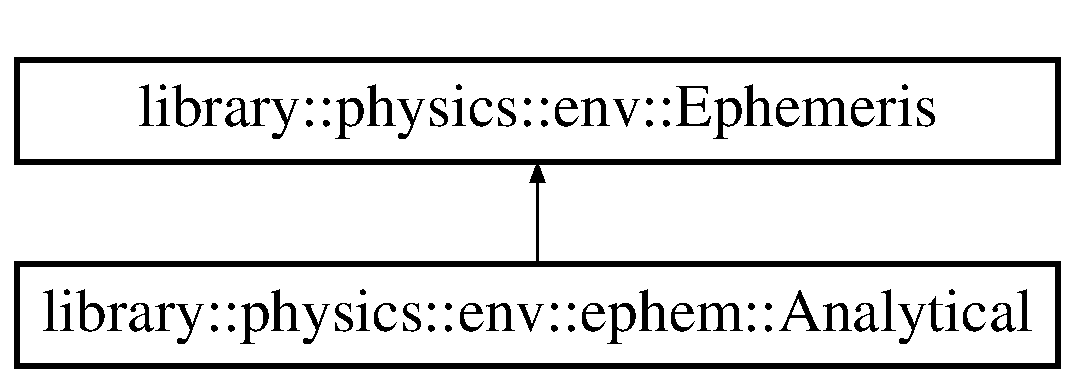
\includegraphics[height=2.000000cm]{classlibrary_1_1physics_1_1env_1_1ephem_1_1_analytical}
\end{center}
\end{figure}
\subsection*{Public Member Functions}
\begin{DoxyCompactItemize}
\item 
\hyperlink{classlibrary_1_1physics_1_1env_1_1ephem_1_1_analytical_a3282f9dfc8fbe95f4b8a7a89141ca60e}{Analytical} (const Shared$<$ const \hyperlink{classlibrary_1_1physics_1_1coord_1_1_frame}{Frame} $>$ \&a\+Frame\+S\+Ptr)
\item 
virtual \hyperlink{classlibrary_1_1physics_1_1env_1_1ephem_1_1_analytical_a0219af2c16308c2e7d39e40ba57fa11e}{$\sim$\+Analytical} () override
\item 
virtual \hyperlink{classlibrary_1_1physics_1_1env_1_1ephem_1_1_analytical}{Analytical} $\ast$ \hyperlink{classlibrary_1_1physics_1_1env_1_1ephem_1_1_analytical_acd51ca99177b1433b6623829ae003bec}{clone} () const override
\item 
virtual bool \hyperlink{classlibrary_1_1physics_1_1env_1_1ephem_1_1_analytical_a0c0fe5d8326ba439bb0b51e7536ab0fd}{is\+Defined} () const override
\item 
virtual Shared$<$ const \hyperlink{classlibrary_1_1physics_1_1coord_1_1_frame}{Frame} $>$ \hyperlink{classlibrary_1_1physics_1_1env_1_1ephem_1_1_analytical_ad16f575a7804bd29710030289d5630b1}{access\+Frame} () const override
\end{DoxyCompactItemize}


\subsection{Constructor \& Destructor Documentation}
\mbox{\Hypertarget{classlibrary_1_1physics_1_1env_1_1ephem_1_1_analytical_a3282f9dfc8fbe95f4b8a7a89141ca60e}\label{classlibrary_1_1physics_1_1env_1_1ephem_1_1_analytical_a3282f9dfc8fbe95f4b8a7a89141ca60e}} 
\index{library\+::physics\+::env\+::ephem\+::\+Analytical@{library\+::physics\+::env\+::ephem\+::\+Analytical}!Analytical@{Analytical}}
\index{Analytical@{Analytical}!library\+::physics\+::env\+::ephem\+::\+Analytical@{library\+::physics\+::env\+::ephem\+::\+Analytical}}
\subsubsection{\texorpdfstring{Analytical()}{Analytical()}}
{\footnotesize\ttfamily library\+::physics\+::env\+::ephem\+::\+Analytical\+::\+Analytical (\begin{DoxyParamCaption}\item[{const Shared$<$ const \hyperlink{classlibrary_1_1physics_1_1coord_1_1_frame}{Frame} $>$ \&}]{a\+Frame\+S\+Ptr }\end{DoxyParamCaption})}

\mbox{\Hypertarget{classlibrary_1_1physics_1_1env_1_1ephem_1_1_analytical_a0219af2c16308c2e7d39e40ba57fa11e}\label{classlibrary_1_1physics_1_1env_1_1ephem_1_1_analytical_a0219af2c16308c2e7d39e40ba57fa11e}} 
\index{library\+::physics\+::env\+::ephem\+::\+Analytical@{library\+::physics\+::env\+::ephem\+::\+Analytical}!````~Analytical@{$\sim$\+Analytical}}
\index{````~Analytical@{$\sim$\+Analytical}!library\+::physics\+::env\+::ephem\+::\+Analytical@{library\+::physics\+::env\+::ephem\+::\+Analytical}}
\subsubsection{\texorpdfstring{$\sim$\+Analytical()}{~Analytical()}}
{\footnotesize\ttfamily library\+::physics\+::env\+::ephem\+::\+Analytical\+::$\sim$\+Analytical (\begin{DoxyParamCaption}{ }\end{DoxyParamCaption})\hspace{0.3cm}{\ttfamily [override]}, {\ttfamily [virtual]}}



\subsection{Member Function Documentation}
\mbox{\Hypertarget{classlibrary_1_1physics_1_1env_1_1ephem_1_1_analytical_ad16f575a7804bd29710030289d5630b1}\label{classlibrary_1_1physics_1_1env_1_1ephem_1_1_analytical_ad16f575a7804bd29710030289d5630b1}} 
\index{library\+::physics\+::env\+::ephem\+::\+Analytical@{library\+::physics\+::env\+::ephem\+::\+Analytical}!access\+Frame@{access\+Frame}}
\index{access\+Frame@{access\+Frame}!library\+::physics\+::env\+::ephem\+::\+Analytical@{library\+::physics\+::env\+::ephem\+::\+Analytical}}
\subsubsection{\texorpdfstring{access\+Frame()}{accessFrame()}}
{\footnotesize\ttfamily Shared$<$ const \hyperlink{classlibrary_1_1physics_1_1coord_1_1_frame}{Frame} $>$ library\+::physics\+::env\+::ephem\+::\+Analytical\+::access\+Frame (\begin{DoxyParamCaption}{ }\end{DoxyParamCaption}) const\hspace{0.3cm}{\ttfamily [override]}, {\ttfamily [virtual]}}



Implements \hyperlink{classlibrary_1_1physics_1_1env_1_1_ephemeris_ac832f493239ace4d53c1c5130c1dad31}{library\+::physics\+::env\+::\+Ephemeris}.

\mbox{\Hypertarget{classlibrary_1_1physics_1_1env_1_1ephem_1_1_analytical_acd51ca99177b1433b6623829ae003bec}\label{classlibrary_1_1physics_1_1env_1_1ephem_1_1_analytical_acd51ca99177b1433b6623829ae003bec}} 
\index{library\+::physics\+::env\+::ephem\+::\+Analytical@{library\+::physics\+::env\+::ephem\+::\+Analytical}!clone@{clone}}
\index{clone@{clone}!library\+::physics\+::env\+::ephem\+::\+Analytical@{library\+::physics\+::env\+::ephem\+::\+Analytical}}
\subsubsection{\texorpdfstring{clone()}{clone()}}
{\footnotesize\ttfamily \hyperlink{classlibrary_1_1physics_1_1env_1_1ephem_1_1_analytical}{Analytical} $\ast$ library\+::physics\+::env\+::ephem\+::\+Analytical\+::clone (\begin{DoxyParamCaption}{ }\end{DoxyParamCaption}) const\hspace{0.3cm}{\ttfamily [override]}, {\ttfamily [virtual]}}



Implements \hyperlink{classlibrary_1_1physics_1_1env_1_1_ephemeris_a7ddecd88d91f79ff204100eb9607b591}{library\+::physics\+::env\+::\+Ephemeris}.

\mbox{\Hypertarget{classlibrary_1_1physics_1_1env_1_1ephem_1_1_analytical_a0c0fe5d8326ba439bb0b51e7536ab0fd}\label{classlibrary_1_1physics_1_1env_1_1ephem_1_1_analytical_a0c0fe5d8326ba439bb0b51e7536ab0fd}} 
\index{library\+::physics\+::env\+::ephem\+::\+Analytical@{library\+::physics\+::env\+::ephem\+::\+Analytical}!is\+Defined@{is\+Defined}}
\index{is\+Defined@{is\+Defined}!library\+::physics\+::env\+::ephem\+::\+Analytical@{library\+::physics\+::env\+::ephem\+::\+Analytical}}
\subsubsection{\texorpdfstring{is\+Defined()}{isDefined()}}
{\footnotesize\ttfamily bool library\+::physics\+::env\+::ephem\+::\+Analytical\+::is\+Defined (\begin{DoxyParamCaption}{ }\end{DoxyParamCaption}) const\hspace{0.3cm}{\ttfamily [override]}, {\ttfamily [virtual]}}



Implements \hyperlink{classlibrary_1_1physics_1_1env_1_1_ephemeris_abf61a03e24dd146199381db14d1d7c68}{library\+::physics\+::env\+::\+Ephemeris}.



The documentation for this class was generated from the following files\+:\begin{DoxyCompactItemize}
\item 
include/\+Library/\+Physics/\+Environment/\+Ephemerides/\hyperlink{_analytical_8hpp}{Analytical.\+hpp}\item 
src/\+Library/\+Physics/\+Environment/\+Ephemerides/\hyperlink{_analytical_8cpp}{Analytical.\+cpp}\end{DoxyCompactItemize}

\hypertarget{classlibrary_1_1physics_1_1units_1_1_angle}{}\section{library\+:\+:physics\+:\+:units\+:\+:Angle Class Reference}
\label{classlibrary_1_1physics_1_1units_1_1_angle}\index{library\+::physics\+::units\+::\+Angle@{library\+::physics\+::units\+::\+Angle}}


\hyperlink{classlibrary_1_1physics_1_1units_1_1_angle}{Angle}.  




{\ttfamily \#include $<$Angle.\+hpp$>$}

Inheritance diagram for library\+:\+:physics\+:\+:units\+:\+:Angle\+:\begin{figure}[H]
\begin{center}
\leavevmode
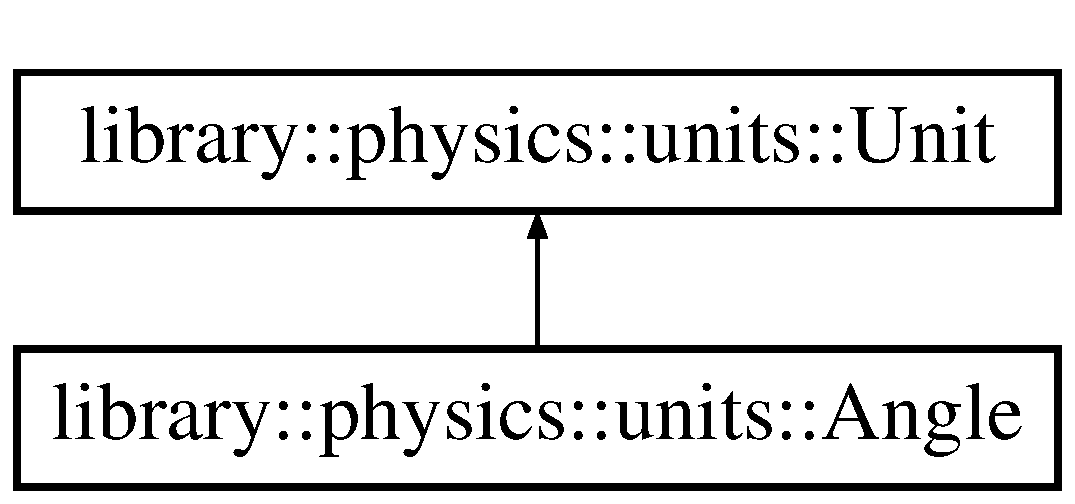
\includegraphics[height=2.000000cm]{classlibrary_1_1physics_1_1units_1_1_angle}
\end{center}
\end{figure}
\subsection*{Public Types}
\begin{DoxyCompactItemize}
\item 
enum \hyperlink{classlibrary_1_1physics_1_1units_1_1_angle_a3c329d415a61783b16ce481874cc5956}{Unit} \{ \newline
\hyperlink{classlibrary_1_1physics_1_1units_1_1_angle_a3c329d415a61783b16ce481874cc5956aec0fc0100c4fc1ce4eea230c3dc10360}{Unit\+::\+Undefined}, 
\hyperlink{classlibrary_1_1physics_1_1units_1_1_angle_a3c329d415a61783b16ce481874cc5956a50c62e3ca8d8ec8732a7f968a3bf2c7c}{Unit\+::\+Radian}, 
\hyperlink{classlibrary_1_1physics_1_1units_1_1_angle_a3c329d415a61783b16ce481874cc5956a6669c4dc00cb161446821b3529ca07d8}{Unit\+::\+Degree}, 
\hyperlink{classlibrary_1_1physics_1_1units_1_1_angle_a3c329d415a61783b16ce481874cc5956a6d59f6ca1b5de72cbdc10a6792bcf090}{Unit\+::\+Arcminute}, 
\newline
\hyperlink{classlibrary_1_1physics_1_1units_1_1_angle_a3c329d415a61783b16ce481874cc5956a7839ceecae19481f2e21e0ce3e11d3aa}{Unit\+::\+Arcsecond}, 
\hyperlink{classlibrary_1_1physics_1_1units_1_1_angle_a3c329d415a61783b16ce481874cc5956aad09b2d48b2811c68e5a2bf421f7f2f2}{Unit\+::\+Revolution}
 \}
\end{DoxyCompactItemize}
\subsection*{Public Member Functions}
\begin{DoxyCompactItemize}
\item 
\hyperlink{classlibrary_1_1physics_1_1units_1_1_angle_a6cd94e306cdc3a15fe13135729299d99}{Angle} (const Real \&a\+Value, const \hyperlink{classlibrary_1_1physics_1_1units_1_1_angle_a3c329d415a61783b16ce481874cc5956}{Angle\+::\+Unit} \&a\+Unit)
\begin{DoxyCompactList}\small\item\em Constructor. \end{DoxyCompactList}\item 
\hyperlink{classlibrary_1_1physics_1_1units_1_1_angle_a6c841e6d88730f6b1289b02dccf591f1}{Angle} (const library\+::math\+::geom\+::\+Angle \&an\+Angle)
\item 
virtual \hyperlink{classlibrary_1_1physics_1_1units_1_1_angle}{Angle} $\ast$ \hyperlink{classlibrary_1_1physics_1_1units_1_1_angle_add51af263128e384d3d89827d0f70dcf}{clone} () const override
\item 
bool \hyperlink{classlibrary_1_1physics_1_1units_1_1_angle_a7438eef61dd54f58c4270fae0d2ccb20}{operator==} (const \hyperlink{classlibrary_1_1physics_1_1units_1_1_angle}{Angle} \&an\+Angle) const
\item 
bool \hyperlink{classlibrary_1_1physics_1_1units_1_1_angle_ad25b468efa92e37f8d45d624a9ed6497}{operator!=} (const \hyperlink{classlibrary_1_1physics_1_1units_1_1_angle}{Angle} \&an\+Angle) const
\item 
\hyperlink{classlibrary_1_1physics_1_1units_1_1_angle}{Angle} \hyperlink{classlibrary_1_1physics_1_1units_1_1_angle_aebf6869b414e02af92a924d561822824}{operator+} (const \hyperlink{classlibrary_1_1physics_1_1units_1_1_angle}{Angle} \&an\+Angle) const
\item 
\hyperlink{classlibrary_1_1physics_1_1units_1_1_angle}{Angle} \hyperlink{classlibrary_1_1physics_1_1units_1_1_angle_a034a88587139bb8642e80f353ead5ce2}{operator-\/} (const \hyperlink{classlibrary_1_1physics_1_1units_1_1_angle}{Angle} \&an\+Angle) const
\item 
\hyperlink{classlibrary_1_1physics_1_1units_1_1_angle}{Angle} \hyperlink{classlibrary_1_1physics_1_1units_1_1_angle_a958b708b331ded088189882187a4de89}{operator$\ast$} (const Real \&a\+Real) const
\item 
\hyperlink{classlibrary_1_1physics_1_1units_1_1_angle}{Angle} \hyperlink{classlibrary_1_1physics_1_1units_1_1_angle_a4807751951c97b1de78e7b98b51abaed}{operator/} (const Real \&a\+Real) const
\item 
\hyperlink{classlibrary_1_1physics_1_1units_1_1_angle}{Angle} \& \hyperlink{classlibrary_1_1physics_1_1units_1_1_angle_a5f20b012cb332e631a6271144a0817a2}{operator+=} (const \hyperlink{classlibrary_1_1physics_1_1units_1_1_angle}{Angle} \&an\+Angle)
\item 
\hyperlink{classlibrary_1_1physics_1_1units_1_1_angle}{Angle} \& \hyperlink{classlibrary_1_1physics_1_1units_1_1_angle_a2278161c893f91578913951c62f29c39}{operator-\/=} (const \hyperlink{classlibrary_1_1physics_1_1units_1_1_angle}{Angle} \&an\+Angle)
\item 
\hyperlink{classlibrary_1_1physics_1_1units_1_1_angle}{Angle} \& \hyperlink{classlibrary_1_1physics_1_1units_1_1_angle_af14d361f18244d859a3829c40aba6a14}{operator$\ast$=} (const Real \&a\+Real)
\item 
\hyperlink{classlibrary_1_1physics_1_1units_1_1_angle}{Angle} \& \hyperlink{classlibrary_1_1physics_1_1units_1_1_angle_a55f228924439a814b8727ae62585df95}{operator/=} (const Real \&a\+Real)
\item 
\hyperlink{classlibrary_1_1physics_1_1units_1_1_angle_a1745d0762e2791835c835e79219b005b}{operator library\+::math\+::geom\+::\+Angle} () const
\item 
virtual bool \hyperlink{classlibrary_1_1physics_1_1units_1_1_angle_a77c7849734ce02b55e070fb88fd87f71}{is\+Defined} () const override
\item 
\hyperlink{classlibrary_1_1physics_1_1units_1_1_angle_a3c329d415a61783b16ce481874cc5956}{Angle\+::\+Unit} \hyperlink{classlibrary_1_1physics_1_1units_1_1_angle_a44ca98d9a05643948f5d3bee79bcba63}{get\+Unit} () const
\item 
Real \hyperlink{classlibrary_1_1physics_1_1units_1_1_angle_aa641b9b6dabfe5fa0b546a2d6492e5be}{in} (const \hyperlink{classlibrary_1_1physics_1_1units_1_1_angle_a3c329d415a61783b16ce481874cc5956}{Angle\+::\+Unit} \&a\+Unit) const
\item 
Real \hyperlink{classlibrary_1_1physics_1_1units_1_1_angle_ab6157462a9d4afe64f4dd11d1b684af9}{in\+Radians} () const
\item 
Real \hyperlink{classlibrary_1_1physics_1_1units_1_1_angle_a6dfbf2ff95818818cecfd60e121dfb75}{in\+Radians} (const Real \&a\+Lower\+Bound, const Real \&an\+Upper\+Bound) const
\item 
Real \hyperlink{classlibrary_1_1physics_1_1units_1_1_angle_a58528bdfdbd6976ee88055809c835e68}{in\+Degrees} () const
\item 
Real \hyperlink{classlibrary_1_1physics_1_1units_1_1_angle_a21fa4d9aa81f1e27d9869e0c8a9cb46b}{in\+Degrees} (const Real \&a\+Lower\+Bound, const Real \&an\+Upper\+Bound) const
\item 
Real \hyperlink{classlibrary_1_1physics_1_1units_1_1_angle_a10195e20b7540e0813c3b2a13c8bf453}{in\+Arcminutes} () const
\item 
Real \hyperlink{classlibrary_1_1physics_1_1units_1_1_angle_a2d16e08281a9745f0da118b56999f313}{in\+Arcminutes} (const Real \&a\+Lower\+Bound, const Real \&an\+Upper\+Bound) const
\item 
Real \hyperlink{classlibrary_1_1physics_1_1units_1_1_angle_af4f0f122d7136c92505a9ec65835815b}{in\+Arcseconds} () const
\item 
Real \hyperlink{classlibrary_1_1physics_1_1units_1_1_angle_acc904a64f693fa07bac55f28c39ba8b4}{in\+Arcseconds} (const Real \&a\+Lower\+Bound, const Real \&an\+Upper\+Bound) const
\item 
Real \hyperlink{classlibrary_1_1physics_1_1units_1_1_angle_a19611fa8ef42050c6ff9724034544d4f}{in\+Revolutions} () const
\item 
virtual String \hyperlink{classlibrary_1_1physics_1_1units_1_1_angle_aae6b7bd4e028ea7719f5a712ca19a86c}{to\+String} (const Integer \&a\+Precision=Integer\+::\+Undefined()) const override
\end{DoxyCompactItemize}
\subsection*{Static Public Member Functions}
\begin{DoxyCompactItemize}
\item 
static \hyperlink{classlibrary_1_1physics_1_1units_1_1_angle}{Angle} \hyperlink{classlibrary_1_1physics_1_1units_1_1_angle_a9c9a16c58d7e1e95e38cf2adf888f334}{Undefined} ()
\item 
static \hyperlink{classlibrary_1_1physics_1_1units_1_1_angle}{Angle} \hyperlink{classlibrary_1_1physics_1_1units_1_1_angle_a3dcf6f9bcee4ae440d36859c30481d2b}{Zero} ()
\item 
static \hyperlink{classlibrary_1_1physics_1_1units_1_1_angle}{Angle} \hyperlink{classlibrary_1_1physics_1_1units_1_1_angle_a921a547ba74630c813201cb2126239cb}{Half\+Pi} ()
\item 
static \hyperlink{classlibrary_1_1physics_1_1units_1_1_angle}{Angle} \hyperlink{classlibrary_1_1physics_1_1units_1_1_angle_a506b763d8a160b8b1ce5fb33a87119a9}{Pi} ()
\item 
static \hyperlink{classlibrary_1_1physics_1_1units_1_1_angle}{Angle} \hyperlink{classlibrary_1_1physics_1_1units_1_1_angle_a7ff0185d33abbb7b3fdcbef1bbb19f74}{Two\+Pi} ()
\item 
static \hyperlink{classlibrary_1_1physics_1_1units_1_1_angle}{Angle} \hyperlink{classlibrary_1_1physics_1_1units_1_1_angle_ac065fbde3c625159cf21153c23c3045b}{Radians} (const Real \&a\+Value)
\item 
static \hyperlink{classlibrary_1_1physics_1_1units_1_1_angle}{Angle} \hyperlink{classlibrary_1_1physics_1_1units_1_1_angle_a20b061534d7d24f807781a06b191603b}{Degrees} (const Real \&a\+Value)
\item 
static \hyperlink{classlibrary_1_1physics_1_1units_1_1_angle}{Angle} \hyperlink{classlibrary_1_1physics_1_1units_1_1_angle_a52f391389a2d59b327b5206e2ee24645}{Arcminutes} (const Real \&a\+Value)
\item 
static \hyperlink{classlibrary_1_1physics_1_1units_1_1_angle}{Angle} \hyperlink{classlibrary_1_1physics_1_1units_1_1_angle_a04df20ae83aa3609c7e7ac5eaf013db9}{Arcseconds} (const Real \&a\+Value)
\item 
static \hyperlink{classlibrary_1_1physics_1_1units_1_1_angle}{Angle} \hyperlink{classlibrary_1_1physics_1_1units_1_1_angle_a2e712e11187dec11a781d457a3f949dc}{Revolutions} (const Real \&a\+Value)
\item 
static \hyperlink{classlibrary_1_1physics_1_1units_1_1_angle}{Angle} \hyperlink{classlibrary_1_1physics_1_1units_1_1_angle_ae12bd433f957f0e297c4d2e5bc3d22cc}{Between} (const Vector2d \&a\+First\+Vector, const Vector2d \&a\+Second\+Vector)
\item 
static \hyperlink{classlibrary_1_1physics_1_1units_1_1_angle}{Angle} \hyperlink{classlibrary_1_1physics_1_1units_1_1_angle_ab7ce400fbca2bfd2ebe453e1685ad049}{Between} (const Vector3d \&a\+First\+Vector, const Vector3d \&a\+Second\+Vector)
\item 
static \hyperlink{classlibrary_1_1physics_1_1units_1_1_angle}{Angle} \hyperlink{classlibrary_1_1physics_1_1units_1_1_angle_a3d7a56d496018330d9529036a31be312}{Parse} (const String \&a\+String)
\item 
static String \hyperlink{classlibrary_1_1physics_1_1units_1_1_angle_a95d8f1d9e27062ca480b7c264a035283}{String\+From\+Unit} (const \hyperlink{classlibrary_1_1physics_1_1units_1_1_angle_a3c329d415a61783b16ce481874cc5956}{Angle\+::\+Unit} \&a\+Unit)
\item 
static String \hyperlink{classlibrary_1_1physics_1_1units_1_1_angle_a2f51939276e1d1c2121e1fc911e6ca30}{Symbol\+From\+Unit} (const \hyperlink{classlibrary_1_1physics_1_1units_1_1_angle_a3c329d415a61783b16ce481874cc5956}{Angle\+::\+Unit} \&a\+Unit)
\end{DoxyCompactItemize}
\subsection*{Friends}
\begin{DoxyCompactItemize}
\item 
\hyperlink{classlibrary_1_1physics_1_1units_1_1_angle}{Angle} \hyperlink{classlibrary_1_1physics_1_1units_1_1_angle_af699984b24759466957ecddaa7e61fc9}{operator$\ast$} (const Real \&a\+Real, const \hyperlink{classlibrary_1_1physics_1_1units_1_1_angle}{Angle} \&an\+Angle)
\item 
std\+::ostream \& \hyperlink{classlibrary_1_1physics_1_1units_1_1_angle_a0846b77ee3281e8a559197c3c3208eed}{operator$<$$<$} (std\+::ostream \&an\+Output\+Stream, const \hyperlink{classlibrary_1_1physics_1_1units_1_1_angle}{Angle} \&an\+Angle)
\end{DoxyCompactItemize}


\subsection{Detailed Description}
\hyperlink{classlibrary_1_1physics_1_1units_1_1_angle}{Angle}. 

In plane geometry, an angle is the figure formed by two rays, called the sides of the angle, sharing a common endpoint, called the vertex of the angle.

https\+://en.wikipedia.\+org/wiki/\+Angle 

\subsection{Member Enumeration Documentation}
\mbox{\Hypertarget{classlibrary_1_1physics_1_1units_1_1_angle_a3c329d415a61783b16ce481874cc5956}\label{classlibrary_1_1physics_1_1units_1_1_angle_a3c329d415a61783b16ce481874cc5956}} 
\index{library\+::physics\+::units\+::\+Angle@{library\+::physics\+::units\+::\+Angle}!Unit@{Unit}}
\index{Unit@{Unit}!library\+::physics\+::units\+::\+Angle@{library\+::physics\+::units\+::\+Angle}}
\subsubsection{\texorpdfstring{Unit}{Unit}}
{\footnotesize\ttfamily enum \hyperlink{classlibrary_1_1physics_1_1units_1_1_angle_a3c329d415a61783b16ce481874cc5956}{library\+::physics\+::units\+::\+Angle\+::\+Unit}\hspace{0.3cm}{\ttfamily [strong]}}

\begin{DoxyEnumFields}{Enumerator}
\raisebox{\heightof{T}}[0pt][0pt]{\index{Undefined@{Undefined}!library\+::physics\+::units\+::\+Angle@{library\+::physics\+::units\+::\+Angle}}\index{library\+::physics\+::units\+::\+Angle@{library\+::physics\+::units\+::\+Angle}!Undefined@{Undefined}}}\mbox{\Hypertarget{classlibrary_1_1physics_1_1units_1_1_angle_a3c329d415a61783b16ce481874cc5956aec0fc0100c4fc1ce4eea230c3dc10360}\label{classlibrary_1_1physics_1_1units_1_1_angle_a3c329d415a61783b16ce481874cc5956aec0fc0100c4fc1ce4eea230c3dc10360}} 
Undefined&Undefined. \\
\hline

\raisebox{\heightof{T}}[0pt][0pt]{\index{Radian@{Radian}!library\+::physics\+::units\+::\+Angle@{library\+::physics\+::units\+::\+Angle}}\index{library\+::physics\+::units\+::\+Angle@{library\+::physics\+::units\+::\+Angle}!Radian@{Radian}}}\mbox{\Hypertarget{classlibrary_1_1physics_1_1units_1_1_angle_a3c329d415a61783b16ce481874cc5956a50c62e3ca8d8ec8732a7f968a3bf2c7c}\label{classlibrary_1_1physics_1_1units_1_1_angle_a3c329d415a61783b16ce481874cc5956a50c62e3ca8d8ec8732a7f968a3bf2c7c}} 
Radian&Radian. \\
\hline

\raisebox{\heightof{T}}[0pt][0pt]{\index{Degree@{Degree}!library\+::physics\+::units\+::\+Angle@{library\+::physics\+::units\+::\+Angle}}\index{library\+::physics\+::units\+::\+Angle@{library\+::physics\+::units\+::\+Angle}!Degree@{Degree}}}\mbox{\Hypertarget{classlibrary_1_1physics_1_1units_1_1_angle_a3c329d415a61783b16ce481874cc5956a6669c4dc00cb161446821b3529ca07d8}\label{classlibrary_1_1physics_1_1units_1_1_angle_a3c329d415a61783b16ce481874cc5956a6669c4dc00cb161446821b3529ca07d8}} 
Degree&Degree. \\
\hline

\raisebox{\heightof{T}}[0pt][0pt]{\index{Arcminute@{Arcminute}!library\+::physics\+::units\+::\+Angle@{library\+::physics\+::units\+::\+Angle}}\index{library\+::physics\+::units\+::\+Angle@{library\+::physics\+::units\+::\+Angle}!Arcminute@{Arcminute}}}\mbox{\Hypertarget{classlibrary_1_1physics_1_1units_1_1_angle_a3c329d415a61783b16ce481874cc5956a6d59f6ca1b5de72cbdc10a6792bcf090}\label{classlibrary_1_1physics_1_1units_1_1_angle_a3c329d415a61783b16ce481874cc5956a6d59f6ca1b5de72cbdc10a6792bcf090}} 
Arcminute&Arcminute. \\
\hline

\raisebox{\heightof{T}}[0pt][0pt]{\index{Arcsecond@{Arcsecond}!library\+::physics\+::units\+::\+Angle@{library\+::physics\+::units\+::\+Angle}}\index{library\+::physics\+::units\+::\+Angle@{library\+::physics\+::units\+::\+Angle}!Arcsecond@{Arcsecond}}}\mbox{\Hypertarget{classlibrary_1_1physics_1_1units_1_1_angle_a3c329d415a61783b16ce481874cc5956a7839ceecae19481f2e21e0ce3e11d3aa}\label{classlibrary_1_1physics_1_1units_1_1_angle_a3c329d415a61783b16ce481874cc5956a7839ceecae19481f2e21e0ce3e11d3aa}} 
Arcsecond&Arcsecond. \\
\hline

\raisebox{\heightof{T}}[0pt][0pt]{\index{Revolution@{Revolution}!library\+::physics\+::units\+::\+Angle@{library\+::physics\+::units\+::\+Angle}}\index{library\+::physics\+::units\+::\+Angle@{library\+::physics\+::units\+::\+Angle}!Revolution@{Revolution}}}\mbox{\Hypertarget{classlibrary_1_1physics_1_1units_1_1_angle_a3c329d415a61783b16ce481874cc5956aad09b2d48b2811c68e5a2bf421f7f2f2}\label{classlibrary_1_1physics_1_1units_1_1_angle_a3c329d415a61783b16ce481874cc5956aad09b2d48b2811c68e5a2bf421f7f2f2}} 
Revolution&Revolution. \\
\hline

\end{DoxyEnumFields}


\subsection{Constructor \& Destructor Documentation}
\mbox{\Hypertarget{classlibrary_1_1physics_1_1units_1_1_angle_a6cd94e306cdc3a15fe13135729299d99}\label{classlibrary_1_1physics_1_1units_1_1_angle_a6cd94e306cdc3a15fe13135729299d99}} 
\index{library\+::physics\+::units\+::\+Angle@{library\+::physics\+::units\+::\+Angle}!Angle@{Angle}}
\index{Angle@{Angle}!library\+::physics\+::units\+::\+Angle@{library\+::physics\+::units\+::\+Angle}}
\subsubsection{\texorpdfstring{Angle()}{Angle()}\hspace{0.1cm}{\footnotesize\ttfamily [1/2]}}
{\footnotesize\ttfamily library\+::physics\+::units\+::\+Angle\+::\+Angle (\begin{DoxyParamCaption}\item[{const Real \&}]{a\+Value,  }\item[{const \hyperlink{classlibrary_1_1physics_1_1units_1_1_angle_a3c329d415a61783b16ce481874cc5956}{Angle\+::\+Unit} \&}]{a\+Unit }\end{DoxyParamCaption})}



Constructor. 


\begin{DoxyCode}
\hyperlink{classlibrary_1_1physics_1_1units_1_1_angle_a6cd94e306cdc3a15fe13135729299d99}{Angle} angle(90.0, \hyperlink{classlibrary_1_1physics_1_1units_1_1_angle_a3c329d415a61783b16ce481874cc5956a6669c4dc00cb161446821b3529ca07d8}{Angle::Unit::Degree}) ;
\end{DoxyCode}



\begin{DoxyParams}[1]{Parameters}
\mbox{\tt in}  & {\em a\+Value} & A value \\
\hline
\mbox{\tt in}  & {\em a\+Unit} & An angle unit \\
\hline
\end{DoxyParams}
\mbox{\Hypertarget{classlibrary_1_1physics_1_1units_1_1_angle_a6c841e6d88730f6b1289b02dccf591f1}\label{classlibrary_1_1physics_1_1units_1_1_angle_a6c841e6d88730f6b1289b02dccf591f1}} 
\index{library\+::physics\+::units\+::\+Angle@{library\+::physics\+::units\+::\+Angle}!Angle@{Angle}}
\index{Angle@{Angle}!library\+::physics\+::units\+::\+Angle@{library\+::physics\+::units\+::\+Angle}}
\subsubsection{\texorpdfstring{Angle()}{Angle()}\hspace{0.1cm}{\footnotesize\ttfamily [2/2]}}
{\footnotesize\ttfamily library\+::physics\+::units\+::\+Angle\+::\+Angle (\begin{DoxyParamCaption}\item[{const library\+::math\+::geom\+::\+Angle \&}]{an\+Angle }\end{DoxyParamCaption})}



\subsection{Member Function Documentation}
\mbox{\Hypertarget{classlibrary_1_1physics_1_1units_1_1_angle_a52f391389a2d59b327b5206e2ee24645}\label{classlibrary_1_1physics_1_1units_1_1_angle_a52f391389a2d59b327b5206e2ee24645}} 
\index{library\+::physics\+::units\+::\+Angle@{library\+::physics\+::units\+::\+Angle}!Arcminutes@{Arcminutes}}
\index{Arcminutes@{Arcminutes}!library\+::physics\+::units\+::\+Angle@{library\+::physics\+::units\+::\+Angle}}
\subsubsection{\texorpdfstring{Arcminutes()}{Arcminutes()}}
{\footnotesize\ttfamily \hyperlink{classlibrary_1_1physics_1_1units_1_1_angle}{Angle} library\+::physics\+::units\+::\+Angle\+::\+Arcminutes (\begin{DoxyParamCaption}\item[{const Real \&}]{a\+Value }\end{DoxyParamCaption})\hspace{0.3cm}{\ttfamily [static]}}

\mbox{\Hypertarget{classlibrary_1_1physics_1_1units_1_1_angle_a04df20ae83aa3609c7e7ac5eaf013db9}\label{classlibrary_1_1physics_1_1units_1_1_angle_a04df20ae83aa3609c7e7ac5eaf013db9}} 
\index{library\+::physics\+::units\+::\+Angle@{library\+::physics\+::units\+::\+Angle}!Arcseconds@{Arcseconds}}
\index{Arcseconds@{Arcseconds}!library\+::physics\+::units\+::\+Angle@{library\+::physics\+::units\+::\+Angle}}
\subsubsection{\texorpdfstring{Arcseconds()}{Arcseconds()}}
{\footnotesize\ttfamily \hyperlink{classlibrary_1_1physics_1_1units_1_1_angle}{Angle} library\+::physics\+::units\+::\+Angle\+::\+Arcseconds (\begin{DoxyParamCaption}\item[{const Real \&}]{a\+Value }\end{DoxyParamCaption})\hspace{0.3cm}{\ttfamily [static]}}

\mbox{\Hypertarget{classlibrary_1_1physics_1_1units_1_1_angle_ae12bd433f957f0e297c4d2e5bc3d22cc}\label{classlibrary_1_1physics_1_1units_1_1_angle_ae12bd433f957f0e297c4d2e5bc3d22cc}} 
\index{library\+::physics\+::units\+::\+Angle@{library\+::physics\+::units\+::\+Angle}!Between@{Between}}
\index{Between@{Between}!library\+::physics\+::units\+::\+Angle@{library\+::physics\+::units\+::\+Angle}}
\subsubsection{\texorpdfstring{Between()}{Between()}\hspace{0.1cm}{\footnotesize\ttfamily [1/2]}}
{\footnotesize\ttfamily \hyperlink{classlibrary_1_1physics_1_1units_1_1_angle}{Angle} library\+::physics\+::units\+::\+Angle\+::\+Between (\begin{DoxyParamCaption}\item[{const Vector2d \&}]{a\+First\+Vector,  }\item[{const Vector2d \&}]{a\+Second\+Vector }\end{DoxyParamCaption})\hspace{0.3cm}{\ttfamily [static]}}

\mbox{\Hypertarget{classlibrary_1_1physics_1_1units_1_1_angle_ab7ce400fbca2bfd2ebe453e1685ad049}\label{classlibrary_1_1physics_1_1units_1_1_angle_ab7ce400fbca2bfd2ebe453e1685ad049}} 
\index{library\+::physics\+::units\+::\+Angle@{library\+::physics\+::units\+::\+Angle}!Between@{Between}}
\index{Between@{Between}!library\+::physics\+::units\+::\+Angle@{library\+::physics\+::units\+::\+Angle}}
\subsubsection{\texorpdfstring{Between()}{Between()}\hspace{0.1cm}{\footnotesize\ttfamily [2/2]}}
{\footnotesize\ttfamily \hyperlink{classlibrary_1_1physics_1_1units_1_1_angle}{Angle} library\+::physics\+::units\+::\+Angle\+::\+Between (\begin{DoxyParamCaption}\item[{const Vector3d \&}]{a\+First\+Vector,  }\item[{const Vector3d \&}]{a\+Second\+Vector }\end{DoxyParamCaption})\hspace{0.3cm}{\ttfamily [static]}}

\mbox{\Hypertarget{classlibrary_1_1physics_1_1units_1_1_angle_add51af263128e384d3d89827d0f70dcf}\label{classlibrary_1_1physics_1_1units_1_1_angle_add51af263128e384d3d89827d0f70dcf}} 
\index{library\+::physics\+::units\+::\+Angle@{library\+::physics\+::units\+::\+Angle}!clone@{clone}}
\index{clone@{clone}!library\+::physics\+::units\+::\+Angle@{library\+::physics\+::units\+::\+Angle}}
\subsubsection{\texorpdfstring{clone()}{clone()}}
{\footnotesize\ttfamily \hyperlink{classlibrary_1_1physics_1_1units_1_1_angle}{Angle} $\ast$ library\+::physics\+::units\+::\+Angle\+::clone (\begin{DoxyParamCaption}{ }\end{DoxyParamCaption}) const\hspace{0.3cm}{\ttfamily [override]}, {\ttfamily [virtual]}}



Implements \hyperlink{classlibrary_1_1physics_1_1units_1_1_unit_aff727141d73acddfae382e5e375f4640}{library\+::physics\+::units\+::\+Unit}.

\mbox{\Hypertarget{classlibrary_1_1physics_1_1units_1_1_angle_a20b061534d7d24f807781a06b191603b}\label{classlibrary_1_1physics_1_1units_1_1_angle_a20b061534d7d24f807781a06b191603b}} 
\index{library\+::physics\+::units\+::\+Angle@{library\+::physics\+::units\+::\+Angle}!Degrees@{Degrees}}
\index{Degrees@{Degrees}!library\+::physics\+::units\+::\+Angle@{library\+::physics\+::units\+::\+Angle}}
\subsubsection{\texorpdfstring{Degrees()}{Degrees()}}
{\footnotesize\ttfamily \hyperlink{classlibrary_1_1physics_1_1units_1_1_angle}{Angle} library\+::physics\+::units\+::\+Angle\+::\+Degrees (\begin{DoxyParamCaption}\item[{const Real \&}]{a\+Value }\end{DoxyParamCaption})\hspace{0.3cm}{\ttfamily [static]}}

\mbox{\Hypertarget{classlibrary_1_1physics_1_1units_1_1_angle_a44ca98d9a05643948f5d3bee79bcba63}\label{classlibrary_1_1physics_1_1units_1_1_angle_a44ca98d9a05643948f5d3bee79bcba63}} 
\index{library\+::physics\+::units\+::\+Angle@{library\+::physics\+::units\+::\+Angle}!get\+Unit@{get\+Unit}}
\index{get\+Unit@{get\+Unit}!library\+::physics\+::units\+::\+Angle@{library\+::physics\+::units\+::\+Angle}}
\subsubsection{\texorpdfstring{get\+Unit()}{getUnit()}}
{\footnotesize\ttfamily \hyperlink{classlibrary_1_1physics_1_1units_1_1_angle_a3c329d415a61783b16ce481874cc5956}{Angle\+::\+Unit} library\+::physics\+::units\+::\+Angle\+::get\+Unit (\begin{DoxyParamCaption}{ }\end{DoxyParamCaption}) const}

\mbox{\Hypertarget{classlibrary_1_1physics_1_1units_1_1_angle_a921a547ba74630c813201cb2126239cb}\label{classlibrary_1_1physics_1_1units_1_1_angle_a921a547ba74630c813201cb2126239cb}} 
\index{library\+::physics\+::units\+::\+Angle@{library\+::physics\+::units\+::\+Angle}!Half\+Pi@{Half\+Pi}}
\index{Half\+Pi@{Half\+Pi}!library\+::physics\+::units\+::\+Angle@{library\+::physics\+::units\+::\+Angle}}
\subsubsection{\texorpdfstring{Half\+Pi()}{HalfPi()}}
{\footnotesize\ttfamily \hyperlink{classlibrary_1_1physics_1_1units_1_1_angle}{Angle} library\+::physics\+::units\+::\+Angle\+::\+Half\+Pi (\begin{DoxyParamCaption}{ }\end{DoxyParamCaption})\hspace{0.3cm}{\ttfamily [static]}}

\mbox{\Hypertarget{classlibrary_1_1physics_1_1units_1_1_angle_aa641b9b6dabfe5fa0b546a2d6492e5be}\label{classlibrary_1_1physics_1_1units_1_1_angle_aa641b9b6dabfe5fa0b546a2d6492e5be}} 
\index{library\+::physics\+::units\+::\+Angle@{library\+::physics\+::units\+::\+Angle}!in@{in}}
\index{in@{in}!library\+::physics\+::units\+::\+Angle@{library\+::physics\+::units\+::\+Angle}}
\subsubsection{\texorpdfstring{in()}{in()}}
{\footnotesize\ttfamily Real library\+::physics\+::units\+::\+Angle\+::in (\begin{DoxyParamCaption}\item[{const \hyperlink{classlibrary_1_1physics_1_1units_1_1_angle_a3c329d415a61783b16ce481874cc5956}{Angle\+::\+Unit} \&}]{a\+Unit }\end{DoxyParamCaption}) const}

\mbox{\Hypertarget{classlibrary_1_1physics_1_1units_1_1_angle_a10195e20b7540e0813c3b2a13c8bf453}\label{classlibrary_1_1physics_1_1units_1_1_angle_a10195e20b7540e0813c3b2a13c8bf453}} 
\index{library\+::physics\+::units\+::\+Angle@{library\+::physics\+::units\+::\+Angle}!in\+Arcminutes@{in\+Arcminutes}}
\index{in\+Arcminutes@{in\+Arcminutes}!library\+::physics\+::units\+::\+Angle@{library\+::physics\+::units\+::\+Angle}}
\subsubsection{\texorpdfstring{in\+Arcminutes()}{inArcminutes()}\hspace{0.1cm}{\footnotesize\ttfamily [1/2]}}
{\footnotesize\ttfamily Real library\+::physics\+::units\+::\+Angle\+::in\+Arcminutes (\begin{DoxyParamCaption}{ }\end{DoxyParamCaption}) const}

\mbox{\Hypertarget{classlibrary_1_1physics_1_1units_1_1_angle_a2d16e08281a9745f0da118b56999f313}\label{classlibrary_1_1physics_1_1units_1_1_angle_a2d16e08281a9745f0da118b56999f313}} 
\index{library\+::physics\+::units\+::\+Angle@{library\+::physics\+::units\+::\+Angle}!in\+Arcminutes@{in\+Arcminutes}}
\index{in\+Arcminutes@{in\+Arcminutes}!library\+::physics\+::units\+::\+Angle@{library\+::physics\+::units\+::\+Angle}}
\subsubsection{\texorpdfstring{in\+Arcminutes()}{inArcminutes()}\hspace{0.1cm}{\footnotesize\ttfamily [2/2]}}
{\footnotesize\ttfamily Real library\+::physics\+::units\+::\+Angle\+::in\+Arcminutes (\begin{DoxyParamCaption}\item[{const Real \&}]{a\+Lower\+Bound,  }\item[{const Real \&}]{an\+Upper\+Bound }\end{DoxyParamCaption}) const}

\mbox{\Hypertarget{classlibrary_1_1physics_1_1units_1_1_angle_af4f0f122d7136c92505a9ec65835815b}\label{classlibrary_1_1physics_1_1units_1_1_angle_af4f0f122d7136c92505a9ec65835815b}} 
\index{library\+::physics\+::units\+::\+Angle@{library\+::physics\+::units\+::\+Angle}!in\+Arcseconds@{in\+Arcseconds}}
\index{in\+Arcseconds@{in\+Arcseconds}!library\+::physics\+::units\+::\+Angle@{library\+::physics\+::units\+::\+Angle}}
\subsubsection{\texorpdfstring{in\+Arcseconds()}{inArcseconds()}\hspace{0.1cm}{\footnotesize\ttfamily [1/2]}}
{\footnotesize\ttfamily Real library\+::physics\+::units\+::\+Angle\+::in\+Arcseconds (\begin{DoxyParamCaption}{ }\end{DoxyParamCaption}) const}

\mbox{\Hypertarget{classlibrary_1_1physics_1_1units_1_1_angle_acc904a64f693fa07bac55f28c39ba8b4}\label{classlibrary_1_1physics_1_1units_1_1_angle_acc904a64f693fa07bac55f28c39ba8b4}} 
\index{library\+::physics\+::units\+::\+Angle@{library\+::physics\+::units\+::\+Angle}!in\+Arcseconds@{in\+Arcseconds}}
\index{in\+Arcseconds@{in\+Arcseconds}!library\+::physics\+::units\+::\+Angle@{library\+::physics\+::units\+::\+Angle}}
\subsubsection{\texorpdfstring{in\+Arcseconds()}{inArcseconds()}\hspace{0.1cm}{\footnotesize\ttfamily [2/2]}}
{\footnotesize\ttfamily Real library\+::physics\+::units\+::\+Angle\+::in\+Arcseconds (\begin{DoxyParamCaption}\item[{const Real \&}]{a\+Lower\+Bound,  }\item[{const Real \&}]{an\+Upper\+Bound }\end{DoxyParamCaption}) const}

\mbox{\Hypertarget{classlibrary_1_1physics_1_1units_1_1_angle_a58528bdfdbd6976ee88055809c835e68}\label{classlibrary_1_1physics_1_1units_1_1_angle_a58528bdfdbd6976ee88055809c835e68}} 
\index{library\+::physics\+::units\+::\+Angle@{library\+::physics\+::units\+::\+Angle}!in\+Degrees@{in\+Degrees}}
\index{in\+Degrees@{in\+Degrees}!library\+::physics\+::units\+::\+Angle@{library\+::physics\+::units\+::\+Angle}}
\subsubsection{\texorpdfstring{in\+Degrees()}{inDegrees()}\hspace{0.1cm}{\footnotesize\ttfamily [1/2]}}
{\footnotesize\ttfamily Real library\+::physics\+::units\+::\+Angle\+::in\+Degrees (\begin{DoxyParamCaption}{ }\end{DoxyParamCaption}) const}

\mbox{\Hypertarget{classlibrary_1_1physics_1_1units_1_1_angle_a21fa4d9aa81f1e27d9869e0c8a9cb46b}\label{classlibrary_1_1physics_1_1units_1_1_angle_a21fa4d9aa81f1e27d9869e0c8a9cb46b}} 
\index{library\+::physics\+::units\+::\+Angle@{library\+::physics\+::units\+::\+Angle}!in\+Degrees@{in\+Degrees}}
\index{in\+Degrees@{in\+Degrees}!library\+::physics\+::units\+::\+Angle@{library\+::physics\+::units\+::\+Angle}}
\subsubsection{\texorpdfstring{in\+Degrees()}{inDegrees()}\hspace{0.1cm}{\footnotesize\ttfamily [2/2]}}
{\footnotesize\ttfamily Real library\+::physics\+::units\+::\+Angle\+::in\+Degrees (\begin{DoxyParamCaption}\item[{const Real \&}]{a\+Lower\+Bound,  }\item[{const Real \&}]{an\+Upper\+Bound }\end{DoxyParamCaption}) const}

\mbox{\Hypertarget{classlibrary_1_1physics_1_1units_1_1_angle_ab6157462a9d4afe64f4dd11d1b684af9}\label{classlibrary_1_1physics_1_1units_1_1_angle_ab6157462a9d4afe64f4dd11d1b684af9}} 
\index{library\+::physics\+::units\+::\+Angle@{library\+::physics\+::units\+::\+Angle}!in\+Radians@{in\+Radians}}
\index{in\+Radians@{in\+Radians}!library\+::physics\+::units\+::\+Angle@{library\+::physics\+::units\+::\+Angle}}
\subsubsection{\texorpdfstring{in\+Radians()}{inRadians()}\hspace{0.1cm}{\footnotesize\ttfamily [1/2]}}
{\footnotesize\ttfamily Real library\+::physics\+::units\+::\+Angle\+::in\+Radians (\begin{DoxyParamCaption}{ }\end{DoxyParamCaption}) const}

\mbox{\Hypertarget{classlibrary_1_1physics_1_1units_1_1_angle_a6dfbf2ff95818818cecfd60e121dfb75}\label{classlibrary_1_1physics_1_1units_1_1_angle_a6dfbf2ff95818818cecfd60e121dfb75}} 
\index{library\+::physics\+::units\+::\+Angle@{library\+::physics\+::units\+::\+Angle}!in\+Radians@{in\+Radians}}
\index{in\+Radians@{in\+Radians}!library\+::physics\+::units\+::\+Angle@{library\+::physics\+::units\+::\+Angle}}
\subsubsection{\texorpdfstring{in\+Radians()}{inRadians()}\hspace{0.1cm}{\footnotesize\ttfamily [2/2]}}
{\footnotesize\ttfamily Real library\+::physics\+::units\+::\+Angle\+::in\+Radians (\begin{DoxyParamCaption}\item[{const Real \&}]{a\+Lower\+Bound,  }\item[{const Real \&}]{an\+Upper\+Bound }\end{DoxyParamCaption}) const}

\mbox{\Hypertarget{classlibrary_1_1physics_1_1units_1_1_angle_a19611fa8ef42050c6ff9724034544d4f}\label{classlibrary_1_1physics_1_1units_1_1_angle_a19611fa8ef42050c6ff9724034544d4f}} 
\index{library\+::physics\+::units\+::\+Angle@{library\+::physics\+::units\+::\+Angle}!in\+Revolutions@{in\+Revolutions}}
\index{in\+Revolutions@{in\+Revolutions}!library\+::physics\+::units\+::\+Angle@{library\+::physics\+::units\+::\+Angle}}
\subsubsection{\texorpdfstring{in\+Revolutions()}{inRevolutions()}}
{\footnotesize\ttfamily Real library\+::physics\+::units\+::\+Angle\+::in\+Revolutions (\begin{DoxyParamCaption}{ }\end{DoxyParamCaption}) const}

\mbox{\Hypertarget{classlibrary_1_1physics_1_1units_1_1_angle_a77c7849734ce02b55e070fb88fd87f71}\label{classlibrary_1_1physics_1_1units_1_1_angle_a77c7849734ce02b55e070fb88fd87f71}} 
\index{library\+::physics\+::units\+::\+Angle@{library\+::physics\+::units\+::\+Angle}!is\+Defined@{is\+Defined}}
\index{is\+Defined@{is\+Defined}!library\+::physics\+::units\+::\+Angle@{library\+::physics\+::units\+::\+Angle}}
\subsubsection{\texorpdfstring{is\+Defined()}{isDefined()}}
{\footnotesize\ttfamily bool library\+::physics\+::units\+::\+Angle\+::is\+Defined (\begin{DoxyParamCaption}{ }\end{DoxyParamCaption}) const\hspace{0.3cm}{\ttfamily [override]}, {\ttfamily [virtual]}}



Reimplemented from \hyperlink{classlibrary_1_1physics_1_1units_1_1_unit_a5ce011c1ffa0fce4cf1f5d42ff06ee78}{library\+::physics\+::units\+::\+Unit}.

\mbox{\Hypertarget{classlibrary_1_1physics_1_1units_1_1_angle_a1745d0762e2791835c835e79219b005b}\label{classlibrary_1_1physics_1_1units_1_1_angle_a1745d0762e2791835c835e79219b005b}} 
\index{library\+::physics\+::units\+::\+Angle@{library\+::physics\+::units\+::\+Angle}!operator library\+::math\+::geom\+::\+Angle@{operator library\+::math\+::geom\+::\+Angle}}
\index{operator library\+::math\+::geom\+::\+Angle@{operator library\+::math\+::geom\+::\+Angle}!library\+::physics\+::units\+::\+Angle@{library\+::physics\+::units\+::\+Angle}}
\subsubsection{\texorpdfstring{operator library\+::math\+::geom\+::\+Angle()}{operator library::math::geom::Angle()}}
{\footnotesize\ttfamily library\+::physics\+::units\+::\+Angle\+::operator library\+::math\+::geom\+::\+Angle (\begin{DoxyParamCaption}{ }\end{DoxyParamCaption}) const}

\mbox{\Hypertarget{classlibrary_1_1physics_1_1units_1_1_angle_ad25b468efa92e37f8d45d624a9ed6497}\label{classlibrary_1_1physics_1_1units_1_1_angle_ad25b468efa92e37f8d45d624a9ed6497}} 
\index{library\+::physics\+::units\+::\+Angle@{library\+::physics\+::units\+::\+Angle}!operator"!=@{operator"!=}}
\index{operator"!=@{operator"!=}!library\+::physics\+::units\+::\+Angle@{library\+::physics\+::units\+::\+Angle}}
\subsubsection{\texorpdfstring{operator"!=()}{operator!=()}}
{\footnotesize\ttfamily bool library\+::physics\+::units\+::\+Angle\+::operator!= (\begin{DoxyParamCaption}\item[{const \hyperlink{classlibrary_1_1physics_1_1units_1_1_angle}{Angle} \&}]{an\+Angle }\end{DoxyParamCaption}) const}

\mbox{\Hypertarget{classlibrary_1_1physics_1_1units_1_1_angle_a958b708b331ded088189882187a4de89}\label{classlibrary_1_1physics_1_1units_1_1_angle_a958b708b331ded088189882187a4de89}} 
\index{library\+::physics\+::units\+::\+Angle@{library\+::physics\+::units\+::\+Angle}!operator$\ast$@{operator$\ast$}}
\index{operator$\ast$@{operator$\ast$}!library\+::physics\+::units\+::\+Angle@{library\+::physics\+::units\+::\+Angle}}
\subsubsection{\texorpdfstring{operator$\ast$()}{operator*()}}
{\footnotesize\ttfamily \hyperlink{classlibrary_1_1physics_1_1units_1_1_angle}{Angle} library\+::physics\+::units\+::\+Angle\+::operator$\ast$ (\begin{DoxyParamCaption}\item[{const Real \&}]{a\+Real }\end{DoxyParamCaption}) const}

\mbox{\Hypertarget{classlibrary_1_1physics_1_1units_1_1_angle_af14d361f18244d859a3829c40aba6a14}\label{classlibrary_1_1physics_1_1units_1_1_angle_af14d361f18244d859a3829c40aba6a14}} 
\index{library\+::physics\+::units\+::\+Angle@{library\+::physics\+::units\+::\+Angle}!operator$\ast$=@{operator$\ast$=}}
\index{operator$\ast$=@{operator$\ast$=}!library\+::physics\+::units\+::\+Angle@{library\+::physics\+::units\+::\+Angle}}
\subsubsection{\texorpdfstring{operator$\ast$=()}{operator*=()}}
{\footnotesize\ttfamily \hyperlink{classlibrary_1_1physics_1_1units_1_1_angle}{Angle} \& library\+::physics\+::units\+::\+Angle\+::operator$\ast$= (\begin{DoxyParamCaption}\item[{const Real \&}]{a\+Real }\end{DoxyParamCaption})}

\mbox{\Hypertarget{classlibrary_1_1physics_1_1units_1_1_angle_aebf6869b414e02af92a924d561822824}\label{classlibrary_1_1physics_1_1units_1_1_angle_aebf6869b414e02af92a924d561822824}} 
\index{library\+::physics\+::units\+::\+Angle@{library\+::physics\+::units\+::\+Angle}!operator+@{operator+}}
\index{operator+@{operator+}!library\+::physics\+::units\+::\+Angle@{library\+::physics\+::units\+::\+Angle}}
\subsubsection{\texorpdfstring{operator+()}{operator+()}}
{\footnotesize\ttfamily \hyperlink{classlibrary_1_1physics_1_1units_1_1_angle}{Angle} library\+::physics\+::units\+::\+Angle\+::operator+ (\begin{DoxyParamCaption}\item[{const \hyperlink{classlibrary_1_1physics_1_1units_1_1_angle}{Angle} \&}]{an\+Angle }\end{DoxyParamCaption}) const}

\mbox{\Hypertarget{classlibrary_1_1physics_1_1units_1_1_angle_a5f20b012cb332e631a6271144a0817a2}\label{classlibrary_1_1physics_1_1units_1_1_angle_a5f20b012cb332e631a6271144a0817a2}} 
\index{library\+::physics\+::units\+::\+Angle@{library\+::physics\+::units\+::\+Angle}!operator+=@{operator+=}}
\index{operator+=@{operator+=}!library\+::physics\+::units\+::\+Angle@{library\+::physics\+::units\+::\+Angle}}
\subsubsection{\texorpdfstring{operator+=()}{operator+=()}}
{\footnotesize\ttfamily \hyperlink{classlibrary_1_1physics_1_1units_1_1_angle}{Angle} \& library\+::physics\+::units\+::\+Angle\+::operator+= (\begin{DoxyParamCaption}\item[{const \hyperlink{classlibrary_1_1physics_1_1units_1_1_angle}{Angle} \&}]{an\+Angle }\end{DoxyParamCaption})}

\mbox{\Hypertarget{classlibrary_1_1physics_1_1units_1_1_angle_a034a88587139bb8642e80f353ead5ce2}\label{classlibrary_1_1physics_1_1units_1_1_angle_a034a88587139bb8642e80f353ead5ce2}} 
\index{library\+::physics\+::units\+::\+Angle@{library\+::physics\+::units\+::\+Angle}!operator-\/@{operator-\/}}
\index{operator-\/@{operator-\/}!library\+::physics\+::units\+::\+Angle@{library\+::physics\+::units\+::\+Angle}}
\subsubsection{\texorpdfstring{operator-\/()}{operator-()}}
{\footnotesize\ttfamily \hyperlink{classlibrary_1_1physics_1_1units_1_1_angle}{Angle} library\+::physics\+::units\+::\+Angle\+::operator-\/ (\begin{DoxyParamCaption}\item[{const \hyperlink{classlibrary_1_1physics_1_1units_1_1_angle}{Angle} \&}]{an\+Angle }\end{DoxyParamCaption}) const}

\mbox{\Hypertarget{classlibrary_1_1physics_1_1units_1_1_angle_a2278161c893f91578913951c62f29c39}\label{classlibrary_1_1physics_1_1units_1_1_angle_a2278161c893f91578913951c62f29c39}} 
\index{library\+::physics\+::units\+::\+Angle@{library\+::physics\+::units\+::\+Angle}!operator-\/=@{operator-\/=}}
\index{operator-\/=@{operator-\/=}!library\+::physics\+::units\+::\+Angle@{library\+::physics\+::units\+::\+Angle}}
\subsubsection{\texorpdfstring{operator-\/=()}{operator-=()}}
{\footnotesize\ttfamily \hyperlink{classlibrary_1_1physics_1_1units_1_1_angle}{Angle} \& library\+::physics\+::units\+::\+Angle\+::operator-\/= (\begin{DoxyParamCaption}\item[{const \hyperlink{classlibrary_1_1physics_1_1units_1_1_angle}{Angle} \&}]{an\+Angle }\end{DoxyParamCaption})}

\mbox{\Hypertarget{classlibrary_1_1physics_1_1units_1_1_angle_a4807751951c97b1de78e7b98b51abaed}\label{classlibrary_1_1physics_1_1units_1_1_angle_a4807751951c97b1de78e7b98b51abaed}} 
\index{library\+::physics\+::units\+::\+Angle@{library\+::physics\+::units\+::\+Angle}!operator/@{operator/}}
\index{operator/@{operator/}!library\+::physics\+::units\+::\+Angle@{library\+::physics\+::units\+::\+Angle}}
\subsubsection{\texorpdfstring{operator/()}{operator/()}}
{\footnotesize\ttfamily \hyperlink{classlibrary_1_1physics_1_1units_1_1_angle}{Angle} library\+::physics\+::units\+::\+Angle\+::operator/ (\begin{DoxyParamCaption}\item[{const Real \&}]{a\+Real }\end{DoxyParamCaption}) const}

\mbox{\Hypertarget{classlibrary_1_1physics_1_1units_1_1_angle_a55f228924439a814b8727ae62585df95}\label{classlibrary_1_1physics_1_1units_1_1_angle_a55f228924439a814b8727ae62585df95}} 
\index{library\+::physics\+::units\+::\+Angle@{library\+::physics\+::units\+::\+Angle}!operator/=@{operator/=}}
\index{operator/=@{operator/=}!library\+::physics\+::units\+::\+Angle@{library\+::physics\+::units\+::\+Angle}}
\subsubsection{\texorpdfstring{operator/=()}{operator/=()}}
{\footnotesize\ttfamily \hyperlink{classlibrary_1_1physics_1_1units_1_1_angle}{Angle} \& library\+::physics\+::units\+::\+Angle\+::operator/= (\begin{DoxyParamCaption}\item[{const Real \&}]{a\+Real }\end{DoxyParamCaption})}

\mbox{\Hypertarget{classlibrary_1_1physics_1_1units_1_1_angle_a7438eef61dd54f58c4270fae0d2ccb20}\label{classlibrary_1_1physics_1_1units_1_1_angle_a7438eef61dd54f58c4270fae0d2ccb20}} 
\index{library\+::physics\+::units\+::\+Angle@{library\+::physics\+::units\+::\+Angle}!operator==@{operator==}}
\index{operator==@{operator==}!library\+::physics\+::units\+::\+Angle@{library\+::physics\+::units\+::\+Angle}}
\subsubsection{\texorpdfstring{operator==()}{operator==()}}
{\footnotesize\ttfamily bool library\+::physics\+::units\+::\+Angle\+::operator== (\begin{DoxyParamCaption}\item[{const \hyperlink{classlibrary_1_1physics_1_1units_1_1_angle}{Angle} \&}]{an\+Angle }\end{DoxyParamCaption}) const}

\mbox{\Hypertarget{classlibrary_1_1physics_1_1units_1_1_angle_a3d7a56d496018330d9529036a31be312}\label{classlibrary_1_1physics_1_1units_1_1_angle_a3d7a56d496018330d9529036a31be312}} 
\index{library\+::physics\+::units\+::\+Angle@{library\+::physics\+::units\+::\+Angle}!Parse@{Parse}}
\index{Parse@{Parse}!library\+::physics\+::units\+::\+Angle@{library\+::physics\+::units\+::\+Angle}}
\subsubsection{\texorpdfstring{Parse()}{Parse()}}
{\footnotesize\ttfamily static \hyperlink{classlibrary_1_1physics_1_1units_1_1_angle}{Angle} library\+::physics\+::units\+::\+Angle\+::\+Parse (\begin{DoxyParamCaption}\item[{const String \&}]{a\+String }\end{DoxyParamCaption})\hspace{0.3cm}{\ttfamily [static]}}

\mbox{\Hypertarget{classlibrary_1_1physics_1_1units_1_1_angle_a506b763d8a160b8b1ce5fb33a87119a9}\label{classlibrary_1_1physics_1_1units_1_1_angle_a506b763d8a160b8b1ce5fb33a87119a9}} 
\index{library\+::physics\+::units\+::\+Angle@{library\+::physics\+::units\+::\+Angle}!Pi@{Pi}}
\index{Pi@{Pi}!library\+::physics\+::units\+::\+Angle@{library\+::physics\+::units\+::\+Angle}}
\subsubsection{\texorpdfstring{Pi()}{Pi()}}
{\footnotesize\ttfamily \hyperlink{classlibrary_1_1physics_1_1units_1_1_angle}{Angle} library\+::physics\+::units\+::\+Angle\+::\+Pi (\begin{DoxyParamCaption}{ }\end{DoxyParamCaption})\hspace{0.3cm}{\ttfamily [static]}}

\mbox{\Hypertarget{classlibrary_1_1physics_1_1units_1_1_angle_ac065fbde3c625159cf21153c23c3045b}\label{classlibrary_1_1physics_1_1units_1_1_angle_ac065fbde3c625159cf21153c23c3045b}} 
\index{library\+::physics\+::units\+::\+Angle@{library\+::physics\+::units\+::\+Angle}!Radians@{Radians}}
\index{Radians@{Radians}!library\+::physics\+::units\+::\+Angle@{library\+::physics\+::units\+::\+Angle}}
\subsubsection{\texorpdfstring{Radians()}{Radians()}}
{\footnotesize\ttfamily \hyperlink{classlibrary_1_1physics_1_1units_1_1_angle}{Angle} library\+::physics\+::units\+::\+Angle\+::\+Radians (\begin{DoxyParamCaption}\item[{const Real \&}]{a\+Value }\end{DoxyParamCaption})\hspace{0.3cm}{\ttfamily [static]}}

\mbox{\Hypertarget{classlibrary_1_1physics_1_1units_1_1_angle_a2e712e11187dec11a781d457a3f949dc}\label{classlibrary_1_1physics_1_1units_1_1_angle_a2e712e11187dec11a781d457a3f949dc}} 
\index{library\+::physics\+::units\+::\+Angle@{library\+::physics\+::units\+::\+Angle}!Revolutions@{Revolutions}}
\index{Revolutions@{Revolutions}!library\+::physics\+::units\+::\+Angle@{library\+::physics\+::units\+::\+Angle}}
\subsubsection{\texorpdfstring{Revolutions()}{Revolutions()}}
{\footnotesize\ttfamily \hyperlink{classlibrary_1_1physics_1_1units_1_1_angle}{Angle} library\+::physics\+::units\+::\+Angle\+::\+Revolutions (\begin{DoxyParamCaption}\item[{const Real \&}]{a\+Value }\end{DoxyParamCaption})\hspace{0.3cm}{\ttfamily [static]}}

\mbox{\Hypertarget{classlibrary_1_1physics_1_1units_1_1_angle_a95d8f1d9e27062ca480b7c264a035283}\label{classlibrary_1_1physics_1_1units_1_1_angle_a95d8f1d9e27062ca480b7c264a035283}} 
\index{library\+::physics\+::units\+::\+Angle@{library\+::physics\+::units\+::\+Angle}!String\+From\+Unit@{String\+From\+Unit}}
\index{String\+From\+Unit@{String\+From\+Unit}!library\+::physics\+::units\+::\+Angle@{library\+::physics\+::units\+::\+Angle}}
\subsubsection{\texorpdfstring{String\+From\+Unit()}{StringFromUnit()}}
{\footnotesize\ttfamily String library\+::physics\+::units\+::\+Angle\+::\+String\+From\+Unit (\begin{DoxyParamCaption}\item[{const \hyperlink{classlibrary_1_1physics_1_1units_1_1_angle_a3c329d415a61783b16ce481874cc5956}{Angle\+::\+Unit} \&}]{a\+Unit }\end{DoxyParamCaption})\hspace{0.3cm}{\ttfamily [static]}}

\mbox{\Hypertarget{classlibrary_1_1physics_1_1units_1_1_angle_a2f51939276e1d1c2121e1fc911e6ca30}\label{classlibrary_1_1physics_1_1units_1_1_angle_a2f51939276e1d1c2121e1fc911e6ca30}} 
\index{library\+::physics\+::units\+::\+Angle@{library\+::physics\+::units\+::\+Angle}!Symbol\+From\+Unit@{Symbol\+From\+Unit}}
\index{Symbol\+From\+Unit@{Symbol\+From\+Unit}!library\+::physics\+::units\+::\+Angle@{library\+::physics\+::units\+::\+Angle}}
\subsubsection{\texorpdfstring{Symbol\+From\+Unit()}{SymbolFromUnit()}}
{\footnotesize\ttfamily String library\+::physics\+::units\+::\+Angle\+::\+Symbol\+From\+Unit (\begin{DoxyParamCaption}\item[{const \hyperlink{classlibrary_1_1physics_1_1units_1_1_angle_a3c329d415a61783b16ce481874cc5956}{Angle\+::\+Unit} \&}]{a\+Unit }\end{DoxyParamCaption})\hspace{0.3cm}{\ttfamily [static]}}

\mbox{\Hypertarget{classlibrary_1_1physics_1_1units_1_1_angle_aae6b7bd4e028ea7719f5a712ca19a86c}\label{classlibrary_1_1physics_1_1units_1_1_angle_aae6b7bd4e028ea7719f5a712ca19a86c}} 
\index{library\+::physics\+::units\+::\+Angle@{library\+::physics\+::units\+::\+Angle}!to\+String@{to\+String}}
\index{to\+String@{to\+String}!library\+::physics\+::units\+::\+Angle@{library\+::physics\+::units\+::\+Angle}}
\subsubsection{\texorpdfstring{to\+String()}{toString()}}
{\footnotesize\ttfamily String library\+::physics\+::units\+::\+Angle\+::to\+String (\begin{DoxyParamCaption}\item[{const Integer \&}]{a\+Precision = {\ttfamily Integer\+:\+:Undefined()} }\end{DoxyParamCaption}) const\hspace{0.3cm}{\ttfamily [override]}, {\ttfamily [virtual]}}



Implements \hyperlink{classlibrary_1_1physics_1_1units_1_1_unit_ad7364d457300e36413323c4aebce8029}{library\+::physics\+::units\+::\+Unit}.

\mbox{\Hypertarget{classlibrary_1_1physics_1_1units_1_1_angle_a7ff0185d33abbb7b3fdcbef1bbb19f74}\label{classlibrary_1_1physics_1_1units_1_1_angle_a7ff0185d33abbb7b3fdcbef1bbb19f74}} 
\index{library\+::physics\+::units\+::\+Angle@{library\+::physics\+::units\+::\+Angle}!Two\+Pi@{Two\+Pi}}
\index{Two\+Pi@{Two\+Pi}!library\+::physics\+::units\+::\+Angle@{library\+::physics\+::units\+::\+Angle}}
\subsubsection{\texorpdfstring{Two\+Pi()}{TwoPi()}}
{\footnotesize\ttfamily \hyperlink{classlibrary_1_1physics_1_1units_1_1_angle}{Angle} library\+::physics\+::units\+::\+Angle\+::\+Two\+Pi (\begin{DoxyParamCaption}{ }\end{DoxyParamCaption})\hspace{0.3cm}{\ttfamily [static]}}

\mbox{\Hypertarget{classlibrary_1_1physics_1_1units_1_1_angle_a9c9a16c58d7e1e95e38cf2adf888f334}\label{classlibrary_1_1physics_1_1units_1_1_angle_a9c9a16c58d7e1e95e38cf2adf888f334}} 
\index{library\+::physics\+::units\+::\+Angle@{library\+::physics\+::units\+::\+Angle}!Undefined@{Undefined}}
\index{Undefined@{Undefined}!library\+::physics\+::units\+::\+Angle@{library\+::physics\+::units\+::\+Angle}}
\subsubsection{\texorpdfstring{Undefined()}{Undefined()}}
{\footnotesize\ttfamily \hyperlink{classlibrary_1_1physics_1_1units_1_1_angle}{Angle} library\+::physics\+::units\+::\+Angle\+::\+Undefined (\begin{DoxyParamCaption}{ }\end{DoxyParamCaption})\hspace{0.3cm}{\ttfamily [static]}}

\mbox{\Hypertarget{classlibrary_1_1physics_1_1units_1_1_angle_a3dcf6f9bcee4ae440d36859c30481d2b}\label{classlibrary_1_1physics_1_1units_1_1_angle_a3dcf6f9bcee4ae440d36859c30481d2b}} 
\index{library\+::physics\+::units\+::\+Angle@{library\+::physics\+::units\+::\+Angle}!Zero@{Zero}}
\index{Zero@{Zero}!library\+::physics\+::units\+::\+Angle@{library\+::physics\+::units\+::\+Angle}}
\subsubsection{\texorpdfstring{Zero()}{Zero()}}
{\footnotesize\ttfamily \hyperlink{classlibrary_1_1physics_1_1units_1_1_angle}{Angle} library\+::physics\+::units\+::\+Angle\+::\+Zero (\begin{DoxyParamCaption}{ }\end{DoxyParamCaption})\hspace{0.3cm}{\ttfamily [static]}}



\subsection{Friends And Related Function Documentation}
\mbox{\Hypertarget{classlibrary_1_1physics_1_1units_1_1_angle_af699984b24759466957ecddaa7e61fc9}\label{classlibrary_1_1physics_1_1units_1_1_angle_af699984b24759466957ecddaa7e61fc9}} 
\index{library\+::physics\+::units\+::\+Angle@{library\+::physics\+::units\+::\+Angle}!operator$\ast$@{operator$\ast$}}
\index{operator$\ast$@{operator$\ast$}!library\+::physics\+::units\+::\+Angle@{library\+::physics\+::units\+::\+Angle}}
\subsubsection{\texorpdfstring{operator$\ast$}{operator*}}
{\footnotesize\ttfamily \hyperlink{classlibrary_1_1physics_1_1units_1_1_angle}{Angle} operator$\ast$ (\begin{DoxyParamCaption}\item[{const Real \&}]{a\+Real,  }\item[{const \hyperlink{classlibrary_1_1physics_1_1units_1_1_angle}{Angle} \&}]{an\+Angle }\end{DoxyParamCaption})\hspace{0.3cm}{\ttfamily [friend]}}

\mbox{\Hypertarget{classlibrary_1_1physics_1_1units_1_1_angle_a0846b77ee3281e8a559197c3c3208eed}\label{classlibrary_1_1physics_1_1units_1_1_angle_a0846b77ee3281e8a559197c3c3208eed}} 
\index{library\+::physics\+::units\+::\+Angle@{library\+::physics\+::units\+::\+Angle}!operator$<$$<$@{operator$<$$<$}}
\index{operator$<$$<$@{operator$<$$<$}!library\+::physics\+::units\+::\+Angle@{library\+::physics\+::units\+::\+Angle}}
\subsubsection{\texorpdfstring{operator$<$$<$}{operator<<}}
{\footnotesize\ttfamily std\+::ostream\& operator$<$$<$ (\begin{DoxyParamCaption}\item[{std\+::ostream \&}]{an\+Output\+Stream,  }\item[{const \hyperlink{classlibrary_1_1physics_1_1units_1_1_angle}{Angle} \&}]{an\+Angle }\end{DoxyParamCaption})\hspace{0.3cm}{\ttfamily [friend]}}



The documentation for this class was generated from the following files\+:\begin{DoxyCompactItemize}
\item 
include/\+Library/\+Physics/\+Units/\+Derived/\hyperlink{_angle_8hpp}{Angle.\+hpp}\item 
src/\+Library/\+Physics/\+Units/\+Derived/\hyperlink{_angle_8cpp}{Angle.\+cpp}\end{DoxyCompactItemize}

\hypertarget{classlibrary_1_1physics_1_1coord_1_1_axes}{}\section{library\+:\+:physics\+:\+:coord\+:\+:Axes Class Reference}
\label{classlibrary_1_1physics_1_1coord_1_1_axes}\index{library\+::physics\+::coord\+::\+Axes@{library\+::physics\+::coord\+::\+Axes}}


\hyperlink{classlibrary_1_1physics_1_1coord_1_1_axes}{Axes}.  




{\ttfamily \#include $<$Axes.\+hpp$>$}

\subsection*{Public Member Functions}
\begin{DoxyCompactItemize}
\item 
\hyperlink{classlibrary_1_1physics_1_1coord_1_1_axes_a1af682b7f36ff1d594e6d93c56f7bf1d}{Axes} (const Vector3d \&a\+X\+Axis, const Vector3d \&a\+Y\+Axis, const Vector3d \&a\+Z\+Axis, const Shared$<$ const \hyperlink{classlibrary_1_1physics_1_1coord_1_1_frame}{Frame} $>$ \&a\+Frame\+S\+Ptr)
\item 
bool \hyperlink{classlibrary_1_1physics_1_1coord_1_1_axes_ace61547b524226237b377644201f62dd}{operator==} (const \hyperlink{classlibrary_1_1physics_1_1coord_1_1_axes}{Axes} \&an\+Axes) const
\item 
bool \hyperlink{classlibrary_1_1physics_1_1coord_1_1_axes_a7732a78df5a460db8a73deb1d736bcc0}{operator!=} (const \hyperlink{classlibrary_1_1physics_1_1coord_1_1_axes}{Axes} \&an\+Axes) const
\item 
bool \hyperlink{classlibrary_1_1physics_1_1coord_1_1_axes_a5f03439d03d6f22449bdea28e22bb074}{is\+Defined} () const
\item 
const Vector3d \& \hyperlink{classlibrary_1_1physics_1_1coord_1_1_axes_acb94f5b4bc9e6cf628635987cfb9c990}{x} () const
\item 
const Vector3d \& \hyperlink{classlibrary_1_1physics_1_1coord_1_1_axes_ae777cb405641d9f71d07ec706787b217}{y} () const
\item 
const Vector3d \& \hyperlink{classlibrary_1_1physics_1_1coord_1_1_axes_a22fa1ae49680fc2c4e8e7e905e472301}{z} () const
\item 
Shared$<$ const \hyperlink{classlibrary_1_1physics_1_1coord_1_1_frame}{Frame} $>$ \hyperlink{classlibrary_1_1physics_1_1coord_1_1_axes_a117493dc268795fd00a785c9cc373259}{get\+Frame} () const
\item 
\hyperlink{classlibrary_1_1physics_1_1coord_1_1_axes}{Axes} \hyperlink{classlibrary_1_1physics_1_1coord_1_1_axes_af2d10c4af1b5b8165f1d75bdd5c3d882}{in\+Frame} (const Shared$<$ const \hyperlink{classlibrary_1_1physics_1_1coord_1_1_frame}{Frame} $>$ \&a\+Frame\+S\+Ptr, const \hyperlink{classlibrary_1_1physics_1_1time_1_1_instant}{Instant} \&an\+Instant) const
\end{DoxyCompactItemize}
\subsection*{Static Public Member Functions}
\begin{DoxyCompactItemize}
\item 
static \hyperlink{classlibrary_1_1physics_1_1coord_1_1_axes}{Axes} \hyperlink{classlibrary_1_1physics_1_1coord_1_1_axes_ab6ed449d3cdd757a42ba5f987c7d5778}{Undefined} ()
\end{DoxyCompactItemize}
\subsection*{Friends}
\begin{DoxyCompactItemize}
\item 
std\+::ostream \& \hyperlink{classlibrary_1_1physics_1_1coord_1_1_axes_a0ed7e604ae11f069877a8ee1a2d9b051}{operator$<$$<$} (std\+::ostream \&an\+Output\+Stream, const \hyperlink{classlibrary_1_1physics_1_1coord_1_1_axes}{Axes} \&an\+Axes)
\end{DoxyCompactItemize}


\subsection{Detailed Description}
\hyperlink{classlibrary_1_1physics_1_1coord_1_1_axes}{Axes}. 

\subsection{Constructor \& Destructor Documentation}
\mbox{\Hypertarget{classlibrary_1_1physics_1_1coord_1_1_axes_a1af682b7f36ff1d594e6d93c56f7bf1d}\label{classlibrary_1_1physics_1_1coord_1_1_axes_a1af682b7f36ff1d594e6d93c56f7bf1d}} 
\index{library\+::physics\+::coord\+::\+Axes@{library\+::physics\+::coord\+::\+Axes}!Axes@{Axes}}
\index{Axes@{Axes}!library\+::physics\+::coord\+::\+Axes@{library\+::physics\+::coord\+::\+Axes}}
\subsubsection{\texorpdfstring{Axes()}{Axes()}}
{\footnotesize\ttfamily library\+::physics\+::coord\+::\+Axes\+::\+Axes (\begin{DoxyParamCaption}\item[{const Vector3d \&}]{a\+X\+Axis,  }\item[{const Vector3d \&}]{a\+Y\+Axis,  }\item[{const Vector3d \&}]{a\+Z\+Axis,  }\item[{const Shared$<$ const \hyperlink{classlibrary_1_1physics_1_1coord_1_1_frame}{Frame} $>$ \&}]{a\+Frame\+S\+Ptr }\end{DoxyParamCaption})}



\subsection{Member Function Documentation}
\mbox{\Hypertarget{classlibrary_1_1physics_1_1coord_1_1_axes_a117493dc268795fd00a785c9cc373259}\label{classlibrary_1_1physics_1_1coord_1_1_axes_a117493dc268795fd00a785c9cc373259}} 
\index{library\+::physics\+::coord\+::\+Axes@{library\+::physics\+::coord\+::\+Axes}!get\+Frame@{get\+Frame}}
\index{get\+Frame@{get\+Frame}!library\+::physics\+::coord\+::\+Axes@{library\+::physics\+::coord\+::\+Axes}}
\subsubsection{\texorpdfstring{get\+Frame()}{getFrame()}}
{\footnotesize\ttfamily Shared$<$ const \hyperlink{classlibrary_1_1physics_1_1coord_1_1_frame}{Frame} $>$ library\+::physics\+::coord\+::\+Axes\+::get\+Frame (\begin{DoxyParamCaption}{ }\end{DoxyParamCaption}) const}

\mbox{\Hypertarget{classlibrary_1_1physics_1_1coord_1_1_axes_af2d10c4af1b5b8165f1d75bdd5c3d882}\label{classlibrary_1_1physics_1_1coord_1_1_axes_af2d10c4af1b5b8165f1d75bdd5c3d882}} 
\index{library\+::physics\+::coord\+::\+Axes@{library\+::physics\+::coord\+::\+Axes}!in\+Frame@{in\+Frame}}
\index{in\+Frame@{in\+Frame}!library\+::physics\+::coord\+::\+Axes@{library\+::physics\+::coord\+::\+Axes}}
\subsubsection{\texorpdfstring{in\+Frame()}{inFrame()}}
{\footnotesize\ttfamily \hyperlink{classlibrary_1_1physics_1_1coord_1_1_axes}{Axes} library\+::physics\+::coord\+::\+Axes\+::in\+Frame (\begin{DoxyParamCaption}\item[{const Shared$<$ const \hyperlink{classlibrary_1_1physics_1_1coord_1_1_frame}{Frame} $>$ \&}]{a\+Frame\+S\+Ptr,  }\item[{const \hyperlink{classlibrary_1_1physics_1_1time_1_1_instant}{Instant} \&}]{an\+Instant }\end{DoxyParamCaption}) const}

\mbox{\Hypertarget{classlibrary_1_1physics_1_1coord_1_1_axes_a5f03439d03d6f22449bdea28e22bb074}\label{classlibrary_1_1physics_1_1coord_1_1_axes_a5f03439d03d6f22449bdea28e22bb074}} 
\index{library\+::physics\+::coord\+::\+Axes@{library\+::physics\+::coord\+::\+Axes}!is\+Defined@{is\+Defined}}
\index{is\+Defined@{is\+Defined}!library\+::physics\+::coord\+::\+Axes@{library\+::physics\+::coord\+::\+Axes}}
\subsubsection{\texorpdfstring{is\+Defined()}{isDefined()}}
{\footnotesize\ttfamily bool library\+::physics\+::coord\+::\+Axes\+::is\+Defined (\begin{DoxyParamCaption}{ }\end{DoxyParamCaption}) const}

\mbox{\Hypertarget{classlibrary_1_1physics_1_1coord_1_1_axes_a7732a78df5a460db8a73deb1d736bcc0}\label{classlibrary_1_1physics_1_1coord_1_1_axes_a7732a78df5a460db8a73deb1d736bcc0}} 
\index{library\+::physics\+::coord\+::\+Axes@{library\+::physics\+::coord\+::\+Axes}!operator"!=@{operator"!=}}
\index{operator"!=@{operator"!=}!library\+::physics\+::coord\+::\+Axes@{library\+::physics\+::coord\+::\+Axes}}
\subsubsection{\texorpdfstring{operator"!=()}{operator!=()}}
{\footnotesize\ttfamily bool library\+::physics\+::coord\+::\+Axes\+::operator!= (\begin{DoxyParamCaption}\item[{const \hyperlink{classlibrary_1_1physics_1_1coord_1_1_axes}{Axes} \&}]{an\+Axes }\end{DoxyParamCaption}) const}

\mbox{\Hypertarget{classlibrary_1_1physics_1_1coord_1_1_axes_ace61547b524226237b377644201f62dd}\label{classlibrary_1_1physics_1_1coord_1_1_axes_ace61547b524226237b377644201f62dd}} 
\index{library\+::physics\+::coord\+::\+Axes@{library\+::physics\+::coord\+::\+Axes}!operator==@{operator==}}
\index{operator==@{operator==}!library\+::physics\+::coord\+::\+Axes@{library\+::physics\+::coord\+::\+Axes}}
\subsubsection{\texorpdfstring{operator==()}{operator==()}}
{\footnotesize\ttfamily bool library\+::physics\+::coord\+::\+Axes\+::operator== (\begin{DoxyParamCaption}\item[{const \hyperlink{classlibrary_1_1physics_1_1coord_1_1_axes}{Axes} \&}]{an\+Axes }\end{DoxyParamCaption}) const}

\mbox{\Hypertarget{classlibrary_1_1physics_1_1coord_1_1_axes_ab6ed449d3cdd757a42ba5f987c7d5778}\label{classlibrary_1_1physics_1_1coord_1_1_axes_ab6ed449d3cdd757a42ba5f987c7d5778}} 
\index{library\+::physics\+::coord\+::\+Axes@{library\+::physics\+::coord\+::\+Axes}!Undefined@{Undefined}}
\index{Undefined@{Undefined}!library\+::physics\+::coord\+::\+Axes@{library\+::physics\+::coord\+::\+Axes}}
\subsubsection{\texorpdfstring{Undefined()}{Undefined()}}
{\footnotesize\ttfamily \hyperlink{classlibrary_1_1physics_1_1coord_1_1_axes}{Axes} library\+::physics\+::coord\+::\+Axes\+::\+Undefined (\begin{DoxyParamCaption}{ }\end{DoxyParamCaption})\hspace{0.3cm}{\ttfamily [static]}}

\mbox{\Hypertarget{classlibrary_1_1physics_1_1coord_1_1_axes_acb94f5b4bc9e6cf628635987cfb9c990}\label{classlibrary_1_1physics_1_1coord_1_1_axes_acb94f5b4bc9e6cf628635987cfb9c990}} 
\index{library\+::physics\+::coord\+::\+Axes@{library\+::physics\+::coord\+::\+Axes}!x@{x}}
\index{x@{x}!library\+::physics\+::coord\+::\+Axes@{library\+::physics\+::coord\+::\+Axes}}
\subsubsection{\texorpdfstring{x()}{x()}}
{\footnotesize\ttfamily const Vector3d \& library\+::physics\+::coord\+::\+Axes\+::x (\begin{DoxyParamCaption}{ }\end{DoxyParamCaption}) const}

\mbox{\Hypertarget{classlibrary_1_1physics_1_1coord_1_1_axes_ae777cb405641d9f71d07ec706787b217}\label{classlibrary_1_1physics_1_1coord_1_1_axes_ae777cb405641d9f71d07ec706787b217}} 
\index{library\+::physics\+::coord\+::\+Axes@{library\+::physics\+::coord\+::\+Axes}!y@{y}}
\index{y@{y}!library\+::physics\+::coord\+::\+Axes@{library\+::physics\+::coord\+::\+Axes}}
\subsubsection{\texorpdfstring{y()}{y()}}
{\footnotesize\ttfamily const Vector3d \& library\+::physics\+::coord\+::\+Axes\+::y (\begin{DoxyParamCaption}{ }\end{DoxyParamCaption}) const}

\mbox{\Hypertarget{classlibrary_1_1physics_1_1coord_1_1_axes_a22fa1ae49680fc2c4e8e7e905e472301}\label{classlibrary_1_1physics_1_1coord_1_1_axes_a22fa1ae49680fc2c4e8e7e905e472301}} 
\index{library\+::physics\+::coord\+::\+Axes@{library\+::physics\+::coord\+::\+Axes}!z@{z}}
\index{z@{z}!library\+::physics\+::coord\+::\+Axes@{library\+::physics\+::coord\+::\+Axes}}
\subsubsection{\texorpdfstring{z()}{z()}}
{\footnotesize\ttfamily const Vector3d \& library\+::physics\+::coord\+::\+Axes\+::z (\begin{DoxyParamCaption}{ }\end{DoxyParamCaption}) const}



\subsection{Friends And Related Function Documentation}
\mbox{\Hypertarget{classlibrary_1_1physics_1_1coord_1_1_axes_a0ed7e604ae11f069877a8ee1a2d9b051}\label{classlibrary_1_1physics_1_1coord_1_1_axes_a0ed7e604ae11f069877a8ee1a2d9b051}} 
\index{library\+::physics\+::coord\+::\+Axes@{library\+::physics\+::coord\+::\+Axes}!operator$<$$<$@{operator$<$$<$}}
\index{operator$<$$<$@{operator$<$$<$}!library\+::physics\+::coord\+::\+Axes@{library\+::physics\+::coord\+::\+Axes}}
\subsubsection{\texorpdfstring{operator$<$$<$}{operator<<}}
{\footnotesize\ttfamily std\+::ostream\& operator$<$$<$ (\begin{DoxyParamCaption}\item[{std\+::ostream \&}]{an\+Output\+Stream,  }\item[{const \hyperlink{classlibrary_1_1physics_1_1coord_1_1_axes}{Axes} \&}]{an\+Axes }\end{DoxyParamCaption})\hspace{0.3cm}{\ttfamily [friend]}}



The documentation for this class was generated from the following files\+:\begin{DoxyCompactItemize}
\item 
include/\+Library/\+Physics/\+Coordinate/\hyperlink{_axes_8hpp}{Axes.\+hpp}\item 
src/\+Library/\+Physics/\+Coordinate/\hyperlink{_axes_8cpp}{Axes.\+cpp}\end{DoxyCompactItemize}

\hypertarget{classlibrary_1_1physics_1_1coord_1_1frame_1_1provider_1_1iers_1_1_bulletin_a}{}\section{library\+:\+:physics\+:\+:coord\+:\+:frame\+:\+:provider\+:\+:iers\+:\+:BulletinA Class Reference}
\label{classlibrary_1_1physics_1_1coord_1_1frame_1_1provider_1_1iers_1_1_bulletin_a}\index{library\+::physics\+::coord\+::frame\+::provider\+::iers\+::\+BulletinA@{library\+::physics\+::coord\+::frame\+::provider\+::iers\+::\+BulletinA}}


I\+E\+RS Bulletin A.  




{\ttfamily \#include $<$Bulletin\+A.\+hpp$>$}

\subsection*{Classes}
\begin{DoxyCompactItemize}
\item 
struct \hyperlink{structlibrary_1_1physics_1_1coord_1_1frame_1_1provider_1_1iers_1_1_bulletin_a_1_1_observation}{Observation}
\item 
struct \hyperlink{structlibrary_1_1physics_1_1coord_1_1frame_1_1provider_1_1iers_1_1_bulletin_a_1_1_prediction}{Prediction}
\end{DoxyCompactItemize}
\subsection*{Public Member Functions}
\begin{DoxyCompactItemize}
\item 
bool \hyperlink{classlibrary_1_1physics_1_1coord_1_1frame_1_1provider_1_1iers_1_1_bulletin_a_a7e56a92bd3c47f77f988c3f9500ffefc}{is\+Defined} () const
\item 
const \hyperlink{classlibrary_1_1physics_1_1time_1_1_date}{Date} \& \hyperlink{classlibrary_1_1physics_1_1coord_1_1frame_1_1provider_1_1iers_1_1_bulletin_a_ad41457e1328a3027e0295981aa755459}{access\+Release\+Date} () const
\item 
const \hyperlink{classlibrary_1_1physics_1_1time_1_1_duration}{Duration} \& \hyperlink{classlibrary_1_1physics_1_1coord_1_1frame_1_1provider_1_1iers_1_1_bulletin_a_a2328367e563496c0e1ae9f6f24821503}{access\+T\+A\+I\+Minus\+U\+TC} () const
\item 
const \hyperlink{classlibrary_1_1physics_1_1time_1_1_instant}{Instant} \& \hyperlink{classlibrary_1_1physics_1_1coord_1_1frame_1_1provider_1_1iers_1_1_bulletin_a_a7d6e2b9004b8850d7d0d3c0524a46a10}{access\+T\+A\+I\+Minus\+U\+T\+C\+Epoch} () const
\item 
const \hyperlink{classlibrary_1_1physics_1_1time_1_1_interval}{Interval} \& \hyperlink{classlibrary_1_1physics_1_1coord_1_1frame_1_1provider_1_1iers_1_1_bulletin_a_aa11bd395146f5fba123269de30353bcc}{access\+Observation\+Interval} () const
\item 
const \hyperlink{classlibrary_1_1physics_1_1time_1_1_interval}{Interval} \& \hyperlink{classlibrary_1_1physics_1_1coord_1_1frame_1_1provider_1_1iers_1_1_bulletin_a_ac453fc509ca657946ad41b9f88e8656d}{access\+Prediction\+Interval} () const
\item 
\hyperlink{classlibrary_1_1physics_1_1time_1_1_date}{Date} \hyperlink{classlibrary_1_1physics_1_1coord_1_1frame_1_1provider_1_1iers_1_1_bulletin_a_a8edff3ac319832dfa9db166aace216d7}{get\+Release\+Date} () const
\item 
\hyperlink{classlibrary_1_1physics_1_1time_1_1_duration}{Duration} \hyperlink{classlibrary_1_1physics_1_1coord_1_1frame_1_1provider_1_1iers_1_1_bulletin_a_a540ee167693ac43cd715dcbdd4347211}{get\+T\+A\+I\+Minus\+U\+TC} () const
\item 
\hyperlink{classlibrary_1_1physics_1_1time_1_1_instant}{Instant} \hyperlink{classlibrary_1_1physics_1_1coord_1_1frame_1_1provider_1_1iers_1_1_bulletin_a_a996dda347950138037ac2e5f5311d385}{get\+T\+A\+I\+Minus\+U\+T\+C\+Epoch} () const
\item 
\hyperlink{classlibrary_1_1physics_1_1time_1_1_interval}{Interval} \hyperlink{classlibrary_1_1physics_1_1coord_1_1frame_1_1provider_1_1iers_1_1_bulletin_a_a0247d07abbaec7888d2193a3a775e857}{get\+Observation\+Interval} () const
\item 
\hyperlink{structlibrary_1_1physics_1_1coord_1_1frame_1_1provider_1_1iers_1_1_bulletin_a_1_1_observation}{Bulletin\+A\+::\+Observation} \hyperlink{classlibrary_1_1physics_1_1coord_1_1frame_1_1provider_1_1iers_1_1_bulletin_a_acbe6d5cd2384b12d20d7b2785703df8d}{get\+Observation\+At} (const \hyperlink{classlibrary_1_1physics_1_1time_1_1_instant}{Instant} \&an\+Instant) const
\item 
\hyperlink{classlibrary_1_1physics_1_1time_1_1_interval}{Interval} \hyperlink{classlibrary_1_1physics_1_1coord_1_1frame_1_1provider_1_1iers_1_1_bulletin_a_a45e03c13ae141de584df7c184205338f}{get\+Prediction\+Interval} () const
\item 
\hyperlink{structlibrary_1_1physics_1_1coord_1_1frame_1_1provider_1_1iers_1_1_bulletin_a_1_1_prediction}{Bulletin\+A\+::\+Prediction} \hyperlink{classlibrary_1_1physics_1_1coord_1_1frame_1_1provider_1_1iers_1_1_bulletin_a_a915f6c004a2e65b60638590354ba4b0e}{get\+Prediction\+At} (const \hyperlink{classlibrary_1_1physics_1_1time_1_1_instant}{Instant} \&an\+Instant) const
\end{DoxyCompactItemize}
\subsection*{Static Public Member Functions}
\begin{DoxyCompactItemize}
\item 
static \hyperlink{classlibrary_1_1physics_1_1coord_1_1frame_1_1provider_1_1iers_1_1_bulletin_a}{BulletinA} \hyperlink{classlibrary_1_1physics_1_1coord_1_1frame_1_1provider_1_1iers_1_1_bulletin_a_a4ac08ec1e1695cab3c253b04a96df2bb}{Undefined} ()
\item 
static \hyperlink{classlibrary_1_1physics_1_1coord_1_1frame_1_1provider_1_1iers_1_1_bulletin_a}{BulletinA} \hyperlink{classlibrary_1_1physics_1_1coord_1_1frame_1_1provider_1_1iers_1_1_bulletin_a_ae261db430e297bd1e5db4bb96e0a23bf}{Load} (const fs\+::\+File \&a\+File)
\end{DoxyCompactItemize}
\subsection*{Friends}
\begin{DoxyCompactItemize}
\item 
std\+::ostream \& \hyperlink{classlibrary_1_1physics_1_1coord_1_1frame_1_1provider_1_1iers_1_1_bulletin_a_ad02d4bd47c889c76484ba4056cee01a4}{operator$<$$<$} (std\+::ostream \&an\+Output\+Stream, const \hyperlink{classlibrary_1_1physics_1_1coord_1_1frame_1_1provider_1_1iers_1_1_bulletin_a}{BulletinA} \&a\+BulletinA)
\end{DoxyCompactItemize}


\subsection{Detailed Description}
I\+E\+RS Bulletin A. 

I\+E\+RS Bulletin A contains Earth orientation parameters x/y pole, U\+T1-\/\+U\+TC and their errors at daily intervals and predictions for 1 year into the future.

The contents of I\+E\+RS Bulletin A are divided into four sections\+:


\begin{DoxyEnumerate}
\item General information including key definitions and the most recently adopted values of D\+U\+T1 and T\+A\+I-\/\+U\+TC.
\item Quick-\/look daily estimates of the E\+O\+Ps determined by smoothing the observed data. This involves the application of systematic corrections and statistical weighting. The results are published with a delay of about one to three days between the date of publication and the last available date with estimated E\+OP.
\item Predictions of x, y, and U\+T1-\/\+U\+TC, up to 365 days following the last day of data. The predictions use similar algorithms based on seasonal filtering and autoregressive processing for x, y, and U\+T1.
\item The combination series for the celestial pole offsets. Bulletin A contains celestial pole offsets with respect to the I\+A\+U1980 Nutation theroy (dpsi and deps) and the I\+AU 2000 Resolutions (dX and dY), beginning on 1 January 2003.
\end{DoxyEnumerate}

http\+://maia.usno.\+navy.\+mil/ser7/ser7.dat 

\subsection{Member Function Documentation}
\mbox{\Hypertarget{classlibrary_1_1physics_1_1coord_1_1frame_1_1provider_1_1iers_1_1_bulletin_a_aa11bd395146f5fba123269de30353bcc}\label{classlibrary_1_1physics_1_1coord_1_1frame_1_1provider_1_1iers_1_1_bulletin_a_aa11bd395146f5fba123269de30353bcc}} 
\index{library\+::physics\+::coord\+::frame\+::provider\+::iers\+::\+BulletinA@{library\+::physics\+::coord\+::frame\+::provider\+::iers\+::\+BulletinA}!access\+Observation\+Interval@{access\+Observation\+Interval}}
\index{access\+Observation\+Interval@{access\+Observation\+Interval}!library\+::physics\+::coord\+::frame\+::provider\+::iers\+::\+BulletinA@{library\+::physics\+::coord\+::frame\+::provider\+::iers\+::\+BulletinA}}
\subsubsection{\texorpdfstring{access\+Observation\+Interval()}{accessObservationInterval()}}
{\footnotesize\ttfamily const \hyperlink{classlibrary_1_1physics_1_1time_1_1_interval}{Interval} \& library\+::physics\+::coord\+::frame\+::provider\+::iers\+::\+Bulletin\+A\+::access\+Observation\+Interval (\begin{DoxyParamCaption}{ }\end{DoxyParamCaption}) const}

\mbox{\Hypertarget{classlibrary_1_1physics_1_1coord_1_1frame_1_1provider_1_1iers_1_1_bulletin_a_ac453fc509ca657946ad41b9f88e8656d}\label{classlibrary_1_1physics_1_1coord_1_1frame_1_1provider_1_1iers_1_1_bulletin_a_ac453fc509ca657946ad41b9f88e8656d}} 
\index{library\+::physics\+::coord\+::frame\+::provider\+::iers\+::\+BulletinA@{library\+::physics\+::coord\+::frame\+::provider\+::iers\+::\+BulletinA}!access\+Prediction\+Interval@{access\+Prediction\+Interval}}
\index{access\+Prediction\+Interval@{access\+Prediction\+Interval}!library\+::physics\+::coord\+::frame\+::provider\+::iers\+::\+BulletinA@{library\+::physics\+::coord\+::frame\+::provider\+::iers\+::\+BulletinA}}
\subsubsection{\texorpdfstring{access\+Prediction\+Interval()}{accessPredictionInterval()}}
{\footnotesize\ttfamily const \hyperlink{classlibrary_1_1physics_1_1time_1_1_interval}{Interval} \& library\+::physics\+::coord\+::frame\+::provider\+::iers\+::\+Bulletin\+A\+::access\+Prediction\+Interval (\begin{DoxyParamCaption}{ }\end{DoxyParamCaption}) const}

\mbox{\Hypertarget{classlibrary_1_1physics_1_1coord_1_1frame_1_1provider_1_1iers_1_1_bulletin_a_ad41457e1328a3027e0295981aa755459}\label{classlibrary_1_1physics_1_1coord_1_1frame_1_1provider_1_1iers_1_1_bulletin_a_ad41457e1328a3027e0295981aa755459}} 
\index{library\+::physics\+::coord\+::frame\+::provider\+::iers\+::\+BulletinA@{library\+::physics\+::coord\+::frame\+::provider\+::iers\+::\+BulletinA}!access\+Release\+Date@{access\+Release\+Date}}
\index{access\+Release\+Date@{access\+Release\+Date}!library\+::physics\+::coord\+::frame\+::provider\+::iers\+::\+BulletinA@{library\+::physics\+::coord\+::frame\+::provider\+::iers\+::\+BulletinA}}
\subsubsection{\texorpdfstring{access\+Release\+Date()}{accessReleaseDate()}}
{\footnotesize\ttfamily const \hyperlink{classlibrary_1_1physics_1_1time_1_1_date}{Date} \& library\+::physics\+::coord\+::frame\+::provider\+::iers\+::\+Bulletin\+A\+::access\+Release\+Date (\begin{DoxyParamCaption}{ }\end{DoxyParamCaption}) const}

\mbox{\Hypertarget{classlibrary_1_1physics_1_1coord_1_1frame_1_1provider_1_1iers_1_1_bulletin_a_a2328367e563496c0e1ae9f6f24821503}\label{classlibrary_1_1physics_1_1coord_1_1frame_1_1provider_1_1iers_1_1_bulletin_a_a2328367e563496c0e1ae9f6f24821503}} 
\index{library\+::physics\+::coord\+::frame\+::provider\+::iers\+::\+BulletinA@{library\+::physics\+::coord\+::frame\+::provider\+::iers\+::\+BulletinA}!access\+T\+A\+I\+Minus\+U\+TC@{access\+T\+A\+I\+Minus\+U\+TC}}
\index{access\+T\+A\+I\+Minus\+U\+TC@{access\+T\+A\+I\+Minus\+U\+TC}!library\+::physics\+::coord\+::frame\+::provider\+::iers\+::\+BulletinA@{library\+::physics\+::coord\+::frame\+::provider\+::iers\+::\+BulletinA}}
\subsubsection{\texorpdfstring{access\+T\+A\+I\+Minus\+U\+T\+C()}{accessTAIMinusUTC()}}
{\footnotesize\ttfamily const \hyperlink{classlibrary_1_1physics_1_1time_1_1_duration}{Duration} \& library\+::physics\+::coord\+::frame\+::provider\+::iers\+::\+Bulletin\+A\+::access\+T\+A\+I\+Minus\+U\+TC (\begin{DoxyParamCaption}{ }\end{DoxyParamCaption}) const}

\mbox{\Hypertarget{classlibrary_1_1physics_1_1coord_1_1frame_1_1provider_1_1iers_1_1_bulletin_a_a7d6e2b9004b8850d7d0d3c0524a46a10}\label{classlibrary_1_1physics_1_1coord_1_1frame_1_1provider_1_1iers_1_1_bulletin_a_a7d6e2b9004b8850d7d0d3c0524a46a10}} 
\index{library\+::physics\+::coord\+::frame\+::provider\+::iers\+::\+BulletinA@{library\+::physics\+::coord\+::frame\+::provider\+::iers\+::\+BulletinA}!access\+T\+A\+I\+Minus\+U\+T\+C\+Epoch@{access\+T\+A\+I\+Minus\+U\+T\+C\+Epoch}}
\index{access\+T\+A\+I\+Minus\+U\+T\+C\+Epoch@{access\+T\+A\+I\+Minus\+U\+T\+C\+Epoch}!library\+::physics\+::coord\+::frame\+::provider\+::iers\+::\+BulletinA@{library\+::physics\+::coord\+::frame\+::provider\+::iers\+::\+BulletinA}}
\subsubsection{\texorpdfstring{access\+T\+A\+I\+Minus\+U\+T\+C\+Epoch()}{accessTAIMinusUTCEpoch()}}
{\footnotesize\ttfamily const \hyperlink{classlibrary_1_1physics_1_1time_1_1_instant}{Instant} \& library\+::physics\+::coord\+::frame\+::provider\+::iers\+::\+Bulletin\+A\+::access\+T\+A\+I\+Minus\+U\+T\+C\+Epoch (\begin{DoxyParamCaption}{ }\end{DoxyParamCaption}) const}

\mbox{\Hypertarget{classlibrary_1_1physics_1_1coord_1_1frame_1_1provider_1_1iers_1_1_bulletin_a_acbe6d5cd2384b12d20d7b2785703df8d}\label{classlibrary_1_1physics_1_1coord_1_1frame_1_1provider_1_1iers_1_1_bulletin_a_acbe6d5cd2384b12d20d7b2785703df8d}} 
\index{library\+::physics\+::coord\+::frame\+::provider\+::iers\+::\+BulletinA@{library\+::physics\+::coord\+::frame\+::provider\+::iers\+::\+BulletinA}!get\+Observation\+At@{get\+Observation\+At}}
\index{get\+Observation\+At@{get\+Observation\+At}!library\+::physics\+::coord\+::frame\+::provider\+::iers\+::\+BulletinA@{library\+::physics\+::coord\+::frame\+::provider\+::iers\+::\+BulletinA}}
\subsubsection{\texorpdfstring{get\+Observation\+At()}{getObservationAt()}}
{\footnotesize\ttfamily \hyperlink{structlibrary_1_1physics_1_1coord_1_1frame_1_1provider_1_1iers_1_1_bulletin_a_1_1_observation}{Bulletin\+A\+::\+Observation} library\+::physics\+::coord\+::frame\+::provider\+::iers\+::\+Bulletin\+A\+::get\+Observation\+At (\begin{DoxyParamCaption}\item[{const \hyperlink{classlibrary_1_1physics_1_1time_1_1_instant}{Instant} \&}]{an\+Instant }\end{DoxyParamCaption}) const}

\mbox{\Hypertarget{classlibrary_1_1physics_1_1coord_1_1frame_1_1provider_1_1iers_1_1_bulletin_a_a0247d07abbaec7888d2193a3a775e857}\label{classlibrary_1_1physics_1_1coord_1_1frame_1_1provider_1_1iers_1_1_bulletin_a_a0247d07abbaec7888d2193a3a775e857}} 
\index{library\+::physics\+::coord\+::frame\+::provider\+::iers\+::\+BulletinA@{library\+::physics\+::coord\+::frame\+::provider\+::iers\+::\+BulletinA}!get\+Observation\+Interval@{get\+Observation\+Interval}}
\index{get\+Observation\+Interval@{get\+Observation\+Interval}!library\+::physics\+::coord\+::frame\+::provider\+::iers\+::\+BulletinA@{library\+::physics\+::coord\+::frame\+::provider\+::iers\+::\+BulletinA}}
\subsubsection{\texorpdfstring{get\+Observation\+Interval()}{getObservationInterval()}}
{\footnotesize\ttfamily \hyperlink{classlibrary_1_1physics_1_1time_1_1_interval}{Interval} library\+::physics\+::coord\+::frame\+::provider\+::iers\+::\+Bulletin\+A\+::get\+Observation\+Interval (\begin{DoxyParamCaption}{ }\end{DoxyParamCaption}) const}

\mbox{\Hypertarget{classlibrary_1_1physics_1_1coord_1_1frame_1_1provider_1_1iers_1_1_bulletin_a_a915f6c004a2e65b60638590354ba4b0e}\label{classlibrary_1_1physics_1_1coord_1_1frame_1_1provider_1_1iers_1_1_bulletin_a_a915f6c004a2e65b60638590354ba4b0e}} 
\index{library\+::physics\+::coord\+::frame\+::provider\+::iers\+::\+BulletinA@{library\+::physics\+::coord\+::frame\+::provider\+::iers\+::\+BulletinA}!get\+Prediction\+At@{get\+Prediction\+At}}
\index{get\+Prediction\+At@{get\+Prediction\+At}!library\+::physics\+::coord\+::frame\+::provider\+::iers\+::\+BulletinA@{library\+::physics\+::coord\+::frame\+::provider\+::iers\+::\+BulletinA}}
\subsubsection{\texorpdfstring{get\+Prediction\+At()}{getPredictionAt()}}
{\footnotesize\ttfamily \hyperlink{structlibrary_1_1physics_1_1coord_1_1frame_1_1provider_1_1iers_1_1_bulletin_a_1_1_prediction}{Bulletin\+A\+::\+Prediction} library\+::physics\+::coord\+::frame\+::provider\+::iers\+::\+Bulletin\+A\+::get\+Prediction\+At (\begin{DoxyParamCaption}\item[{const \hyperlink{classlibrary_1_1physics_1_1time_1_1_instant}{Instant} \&}]{an\+Instant }\end{DoxyParamCaption}) const}

\mbox{\Hypertarget{classlibrary_1_1physics_1_1coord_1_1frame_1_1provider_1_1iers_1_1_bulletin_a_a45e03c13ae141de584df7c184205338f}\label{classlibrary_1_1physics_1_1coord_1_1frame_1_1provider_1_1iers_1_1_bulletin_a_a45e03c13ae141de584df7c184205338f}} 
\index{library\+::physics\+::coord\+::frame\+::provider\+::iers\+::\+BulletinA@{library\+::physics\+::coord\+::frame\+::provider\+::iers\+::\+BulletinA}!get\+Prediction\+Interval@{get\+Prediction\+Interval}}
\index{get\+Prediction\+Interval@{get\+Prediction\+Interval}!library\+::physics\+::coord\+::frame\+::provider\+::iers\+::\+BulletinA@{library\+::physics\+::coord\+::frame\+::provider\+::iers\+::\+BulletinA}}
\subsubsection{\texorpdfstring{get\+Prediction\+Interval()}{getPredictionInterval()}}
{\footnotesize\ttfamily \hyperlink{classlibrary_1_1physics_1_1time_1_1_interval}{Interval} library\+::physics\+::coord\+::frame\+::provider\+::iers\+::\+Bulletin\+A\+::get\+Prediction\+Interval (\begin{DoxyParamCaption}{ }\end{DoxyParamCaption}) const}

\mbox{\Hypertarget{classlibrary_1_1physics_1_1coord_1_1frame_1_1provider_1_1iers_1_1_bulletin_a_a8edff3ac319832dfa9db166aace216d7}\label{classlibrary_1_1physics_1_1coord_1_1frame_1_1provider_1_1iers_1_1_bulletin_a_a8edff3ac319832dfa9db166aace216d7}} 
\index{library\+::physics\+::coord\+::frame\+::provider\+::iers\+::\+BulletinA@{library\+::physics\+::coord\+::frame\+::provider\+::iers\+::\+BulletinA}!get\+Release\+Date@{get\+Release\+Date}}
\index{get\+Release\+Date@{get\+Release\+Date}!library\+::physics\+::coord\+::frame\+::provider\+::iers\+::\+BulletinA@{library\+::physics\+::coord\+::frame\+::provider\+::iers\+::\+BulletinA}}
\subsubsection{\texorpdfstring{get\+Release\+Date()}{getReleaseDate()}}
{\footnotesize\ttfamily \hyperlink{classlibrary_1_1physics_1_1time_1_1_date}{Date} library\+::physics\+::coord\+::frame\+::provider\+::iers\+::\+Bulletin\+A\+::get\+Release\+Date (\begin{DoxyParamCaption}{ }\end{DoxyParamCaption}) const}

\mbox{\Hypertarget{classlibrary_1_1physics_1_1coord_1_1frame_1_1provider_1_1iers_1_1_bulletin_a_a540ee167693ac43cd715dcbdd4347211}\label{classlibrary_1_1physics_1_1coord_1_1frame_1_1provider_1_1iers_1_1_bulletin_a_a540ee167693ac43cd715dcbdd4347211}} 
\index{library\+::physics\+::coord\+::frame\+::provider\+::iers\+::\+BulletinA@{library\+::physics\+::coord\+::frame\+::provider\+::iers\+::\+BulletinA}!get\+T\+A\+I\+Minus\+U\+TC@{get\+T\+A\+I\+Minus\+U\+TC}}
\index{get\+T\+A\+I\+Minus\+U\+TC@{get\+T\+A\+I\+Minus\+U\+TC}!library\+::physics\+::coord\+::frame\+::provider\+::iers\+::\+BulletinA@{library\+::physics\+::coord\+::frame\+::provider\+::iers\+::\+BulletinA}}
\subsubsection{\texorpdfstring{get\+T\+A\+I\+Minus\+U\+T\+C()}{getTAIMinusUTC()}}
{\footnotesize\ttfamily \hyperlink{classlibrary_1_1physics_1_1time_1_1_duration}{Duration} library\+::physics\+::coord\+::frame\+::provider\+::iers\+::\+Bulletin\+A\+::get\+T\+A\+I\+Minus\+U\+TC (\begin{DoxyParamCaption}{ }\end{DoxyParamCaption}) const}

\mbox{\Hypertarget{classlibrary_1_1physics_1_1coord_1_1frame_1_1provider_1_1iers_1_1_bulletin_a_a996dda347950138037ac2e5f5311d385}\label{classlibrary_1_1physics_1_1coord_1_1frame_1_1provider_1_1iers_1_1_bulletin_a_a996dda347950138037ac2e5f5311d385}} 
\index{library\+::physics\+::coord\+::frame\+::provider\+::iers\+::\+BulletinA@{library\+::physics\+::coord\+::frame\+::provider\+::iers\+::\+BulletinA}!get\+T\+A\+I\+Minus\+U\+T\+C\+Epoch@{get\+T\+A\+I\+Minus\+U\+T\+C\+Epoch}}
\index{get\+T\+A\+I\+Minus\+U\+T\+C\+Epoch@{get\+T\+A\+I\+Minus\+U\+T\+C\+Epoch}!library\+::physics\+::coord\+::frame\+::provider\+::iers\+::\+BulletinA@{library\+::physics\+::coord\+::frame\+::provider\+::iers\+::\+BulletinA}}
\subsubsection{\texorpdfstring{get\+T\+A\+I\+Minus\+U\+T\+C\+Epoch()}{getTAIMinusUTCEpoch()}}
{\footnotesize\ttfamily \hyperlink{classlibrary_1_1physics_1_1time_1_1_instant}{Instant} library\+::physics\+::coord\+::frame\+::provider\+::iers\+::\+Bulletin\+A\+::get\+T\+A\+I\+Minus\+U\+T\+C\+Epoch (\begin{DoxyParamCaption}{ }\end{DoxyParamCaption}) const}

\mbox{\Hypertarget{classlibrary_1_1physics_1_1coord_1_1frame_1_1provider_1_1iers_1_1_bulletin_a_a7e56a92bd3c47f77f988c3f9500ffefc}\label{classlibrary_1_1physics_1_1coord_1_1frame_1_1provider_1_1iers_1_1_bulletin_a_a7e56a92bd3c47f77f988c3f9500ffefc}} 
\index{library\+::physics\+::coord\+::frame\+::provider\+::iers\+::\+BulletinA@{library\+::physics\+::coord\+::frame\+::provider\+::iers\+::\+BulletinA}!is\+Defined@{is\+Defined}}
\index{is\+Defined@{is\+Defined}!library\+::physics\+::coord\+::frame\+::provider\+::iers\+::\+BulletinA@{library\+::physics\+::coord\+::frame\+::provider\+::iers\+::\+BulletinA}}
\subsubsection{\texorpdfstring{is\+Defined()}{isDefined()}}
{\footnotesize\ttfamily bool library\+::physics\+::coord\+::frame\+::provider\+::iers\+::\+Bulletin\+A\+::is\+Defined (\begin{DoxyParamCaption}{ }\end{DoxyParamCaption}) const}

\mbox{\Hypertarget{classlibrary_1_1physics_1_1coord_1_1frame_1_1provider_1_1iers_1_1_bulletin_a_ae261db430e297bd1e5db4bb96e0a23bf}\label{classlibrary_1_1physics_1_1coord_1_1frame_1_1provider_1_1iers_1_1_bulletin_a_ae261db430e297bd1e5db4bb96e0a23bf}} 
\index{library\+::physics\+::coord\+::frame\+::provider\+::iers\+::\+BulletinA@{library\+::physics\+::coord\+::frame\+::provider\+::iers\+::\+BulletinA}!Load@{Load}}
\index{Load@{Load}!library\+::physics\+::coord\+::frame\+::provider\+::iers\+::\+BulletinA@{library\+::physics\+::coord\+::frame\+::provider\+::iers\+::\+BulletinA}}
\subsubsection{\texorpdfstring{Load()}{Load()}}
{\footnotesize\ttfamily \hyperlink{classlibrary_1_1physics_1_1coord_1_1frame_1_1provider_1_1iers_1_1_bulletin_a}{BulletinA} library\+::physics\+::coord\+::frame\+::provider\+::iers\+::\+Bulletin\+A\+::\+Load (\begin{DoxyParamCaption}\item[{const fs\+::\+File \&}]{a\+File }\end{DoxyParamCaption})\hspace{0.3cm}{\ttfamily [static]}}

\mbox{\Hypertarget{classlibrary_1_1physics_1_1coord_1_1frame_1_1provider_1_1iers_1_1_bulletin_a_a4ac08ec1e1695cab3c253b04a96df2bb}\label{classlibrary_1_1physics_1_1coord_1_1frame_1_1provider_1_1iers_1_1_bulletin_a_a4ac08ec1e1695cab3c253b04a96df2bb}} 
\index{library\+::physics\+::coord\+::frame\+::provider\+::iers\+::\+BulletinA@{library\+::physics\+::coord\+::frame\+::provider\+::iers\+::\+BulletinA}!Undefined@{Undefined}}
\index{Undefined@{Undefined}!library\+::physics\+::coord\+::frame\+::provider\+::iers\+::\+BulletinA@{library\+::physics\+::coord\+::frame\+::provider\+::iers\+::\+BulletinA}}
\subsubsection{\texorpdfstring{Undefined()}{Undefined()}}
{\footnotesize\ttfamily \hyperlink{classlibrary_1_1physics_1_1coord_1_1frame_1_1provider_1_1iers_1_1_bulletin_a}{BulletinA} library\+::physics\+::coord\+::frame\+::provider\+::iers\+::\+Bulletin\+A\+::\+Undefined (\begin{DoxyParamCaption}{ }\end{DoxyParamCaption})\hspace{0.3cm}{\ttfamily [static]}}



\subsection{Friends And Related Function Documentation}
\mbox{\Hypertarget{classlibrary_1_1physics_1_1coord_1_1frame_1_1provider_1_1iers_1_1_bulletin_a_ad02d4bd47c889c76484ba4056cee01a4}\label{classlibrary_1_1physics_1_1coord_1_1frame_1_1provider_1_1iers_1_1_bulletin_a_ad02d4bd47c889c76484ba4056cee01a4}} 
\index{library\+::physics\+::coord\+::frame\+::provider\+::iers\+::\+BulletinA@{library\+::physics\+::coord\+::frame\+::provider\+::iers\+::\+BulletinA}!operator$<$$<$@{operator$<$$<$}}
\index{operator$<$$<$@{operator$<$$<$}!library\+::physics\+::coord\+::frame\+::provider\+::iers\+::\+BulletinA@{library\+::physics\+::coord\+::frame\+::provider\+::iers\+::\+BulletinA}}
\subsubsection{\texorpdfstring{operator$<$$<$}{operator<<}}
{\footnotesize\ttfamily std\+::ostream\& operator$<$$<$ (\begin{DoxyParamCaption}\item[{std\+::ostream \&}]{an\+Output\+Stream,  }\item[{const \hyperlink{classlibrary_1_1physics_1_1coord_1_1frame_1_1provider_1_1iers_1_1_bulletin_a}{BulletinA} \&}]{a\+BulletinA }\end{DoxyParamCaption})\hspace{0.3cm}{\ttfamily [friend]}}



The documentation for this class was generated from the following files\+:\begin{DoxyCompactItemize}
\item 
include/\+Library/\+Physics/\+Coordinate/\+Frame/\+Providers/\+I\+E\+R\+S/\hyperlink{_bulletin_a_8hpp}{Bulletin\+A.\+hpp}\item 
src/\+Library/\+Physics/\+Coordinate/\+Frame/\+Providers/\+I\+E\+R\+S/\hyperlink{_bulletin_a_8cpp}{Bulletin\+A.\+cpp}\end{DoxyCompactItemize}

\hypertarget{classlibrary_1_1physics_1_1coord_1_1frame_1_1provider_1_1iers_1_1_bulletin_b}{}\section{library\+:\+:physics\+:\+:coord\+:\+:frame\+:\+:provider\+:\+:iers\+:\+:BulletinB Class Reference}
\label{classlibrary_1_1physics_1_1coord_1_1frame_1_1provider_1_1iers_1_1_bulletin_b}\index{library\+::physics\+::coord\+::frame\+::provider\+::iers\+::\+BulletinB@{library\+::physics\+::coord\+::frame\+::provider\+::iers\+::\+BulletinB}}


I\+E\+RS Bulletin B.  




{\ttfamily \#include $<$Bulletin\+B.\+hpp$>$}

\subsection*{Public Member Functions}
\begin{DoxyCompactItemize}
\item 
bool \hyperlink{classlibrary_1_1physics_1_1coord_1_1frame_1_1provider_1_1iers_1_1_bulletin_b_ae385502ba4612cdd801c42ddd7f79bb8}{is\+Defined} () const
\end{DoxyCompactItemize}
\subsection*{Static Public Member Functions}
\begin{DoxyCompactItemize}
\item 
static \hyperlink{classlibrary_1_1physics_1_1coord_1_1frame_1_1provider_1_1iers_1_1_bulletin_b}{BulletinB} \hyperlink{classlibrary_1_1physics_1_1coord_1_1frame_1_1provider_1_1iers_1_1_bulletin_b_a6f8a61852b6d83898e3dd800af65e88a}{Undefined} ()
\item 
static \hyperlink{classlibrary_1_1physics_1_1coord_1_1frame_1_1provider_1_1iers_1_1_bulletin_b}{BulletinB} \hyperlink{classlibrary_1_1physics_1_1coord_1_1frame_1_1provider_1_1iers_1_1_bulletin_b_af50be94b68f3eb752f2e5fd8a4f016cd}{Load} (const fs\+::\+File \&a\+File)
\end{DoxyCompactItemize}
\subsection*{Friends}
\begin{DoxyCompactItemize}
\item 
std\+::ostream \& \hyperlink{classlibrary_1_1physics_1_1coord_1_1frame_1_1provider_1_1iers_1_1_bulletin_b_a36d9e78a5de0361186ca1cb63ab6f1ee}{operator$<$$<$} (std\+::ostream \&an\+Output\+Stream, const \hyperlink{classlibrary_1_1physics_1_1coord_1_1frame_1_1provider_1_1iers_1_1_bulletin_b}{BulletinB} \&a\+BulletinB)
\end{DoxyCompactItemize}


\subsection{Detailed Description}
I\+E\+RS Bulletin B. 

I\+E\+RS Bulletin B provides current information on the Earth’s orientation in the I\+E\+RS Reference System. This includes Universal Time, coordinates of the terrestrial pole, and celestial pole offsets. I\+E\+RS Bulletin B consists of 5 sections\+:

Section 1\+: Daily final values at 0\+:00 UT of x, y, U\+T1-\/\+U\+TC, dX, dY, and their uncertainties. Time span\+: one month with final values, one month with preliminary values.

Section 2\+: Daily final values at 0\+:00 UT of celestial pole offsets d\+Psi and d\+Eps in the I\+AU 1980 system and their uncertainties.

Section 3\+: Earth angular velocity (daily estimates of L\+OD and O\+M\+E\+GA with their uncertainties).

Section 4\+: Information on the time scales and announcement of occurring leap seconds.

Section 5\+: Average formal precision of the individual and combined series contributing or not to the combination and their agreement with the combination.

https\+://www.iers.\+org/\+I\+E\+R\+S/\+E\+N/\+Publications/\+Bulletins/bulletins.html 

\subsection{Member Function Documentation}
\mbox{\Hypertarget{classlibrary_1_1physics_1_1coord_1_1frame_1_1provider_1_1iers_1_1_bulletin_b_ae385502ba4612cdd801c42ddd7f79bb8}\label{classlibrary_1_1physics_1_1coord_1_1frame_1_1provider_1_1iers_1_1_bulletin_b_ae385502ba4612cdd801c42ddd7f79bb8}} 
\index{library\+::physics\+::coord\+::frame\+::provider\+::iers\+::\+BulletinB@{library\+::physics\+::coord\+::frame\+::provider\+::iers\+::\+BulletinB}!is\+Defined@{is\+Defined}}
\index{is\+Defined@{is\+Defined}!library\+::physics\+::coord\+::frame\+::provider\+::iers\+::\+BulletinB@{library\+::physics\+::coord\+::frame\+::provider\+::iers\+::\+BulletinB}}
\subsubsection{\texorpdfstring{is\+Defined()}{isDefined()}}
{\footnotesize\ttfamily bool library\+::physics\+::coord\+::frame\+::provider\+::iers\+::\+Bulletin\+B\+::is\+Defined (\begin{DoxyParamCaption}{ }\end{DoxyParamCaption}) const}

\mbox{\Hypertarget{classlibrary_1_1physics_1_1coord_1_1frame_1_1provider_1_1iers_1_1_bulletin_b_af50be94b68f3eb752f2e5fd8a4f016cd}\label{classlibrary_1_1physics_1_1coord_1_1frame_1_1provider_1_1iers_1_1_bulletin_b_af50be94b68f3eb752f2e5fd8a4f016cd}} 
\index{library\+::physics\+::coord\+::frame\+::provider\+::iers\+::\+BulletinB@{library\+::physics\+::coord\+::frame\+::provider\+::iers\+::\+BulletinB}!Load@{Load}}
\index{Load@{Load}!library\+::physics\+::coord\+::frame\+::provider\+::iers\+::\+BulletinB@{library\+::physics\+::coord\+::frame\+::provider\+::iers\+::\+BulletinB}}
\subsubsection{\texorpdfstring{Load()}{Load()}}
{\footnotesize\ttfamily static \hyperlink{classlibrary_1_1physics_1_1coord_1_1frame_1_1provider_1_1iers_1_1_bulletin_b}{BulletinB} library\+::physics\+::coord\+::frame\+::provider\+::iers\+::\+Bulletin\+B\+::\+Load (\begin{DoxyParamCaption}\item[{const fs\+::\+File \&}]{a\+File }\end{DoxyParamCaption})\hspace{0.3cm}{\ttfamily [static]}}

\mbox{\Hypertarget{classlibrary_1_1physics_1_1coord_1_1frame_1_1provider_1_1iers_1_1_bulletin_b_a6f8a61852b6d83898e3dd800af65e88a}\label{classlibrary_1_1physics_1_1coord_1_1frame_1_1provider_1_1iers_1_1_bulletin_b_a6f8a61852b6d83898e3dd800af65e88a}} 
\index{library\+::physics\+::coord\+::frame\+::provider\+::iers\+::\+BulletinB@{library\+::physics\+::coord\+::frame\+::provider\+::iers\+::\+BulletinB}!Undefined@{Undefined}}
\index{Undefined@{Undefined}!library\+::physics\+::coord\+::frame\+::provider\+::iers\+::\+BulletinB@{library\+::physics\+::coord\+::frame\+::provider\+::iers\+::\+BulletinB}}
\subsubsection{\texorpdfstring{Undefined()}{Undefined()}}
{\footnotesize\ttfamily static \hyperlink{classlibrary_1_1physics_1_1coord_1_1frame_1_1provider_1_1iers_1_1_bulletin_b}{BulletinB} library\+::physics\+::coord\+::frame\+::provider\+::iers\+::\+Bulletin\+B\+::\+Undefined (\begin{DoxyParamCaption}{ }\end{DoxyParamCaption})\hspace{0.3cm}{\ttfamily [static]}}



\subsection{Friends And Related Function Documentation}
\mbox{\Hypertarget{classlibrary_1_1physics_1_1coord_1_1frame_1_1provider_1_1iers_1_1_bulletin_b_a36d9e78a5de0361186ca1cb63ab6f1ee}\label{classlibrary_1_1physics_1_1coord_1_1frame_1_1provider_1_1iers_1_1_bulletin_b_a36d9e78a5de0361186ca1cb63ab6f1ee}} 
\index{library\+::physics\+::coord\+::frame\+::provider\+::iers\+::\+BulletinB@{library\+::physics\+::coord\+::frame\+::provider\+::iers\+::\+BulletinB}!operator$<$$<$@{operator$<$$<$}}
\index{operator$<$$<$@{operator$<$$<$}!library\+::physics\+::coord\+::frame\+::provider\+::iers\+::\+BulletinB@{library\+::physics\+::coord\+::frame\+::provider\+::iers\+::\+BulletinB}}
\subsubsection{\texorpdfstring{operator$<$$<$}{operator<<}}
{\footnotesize\ttfamily std\+::ostream\& operator$<$$<$ (\begin{DoxyParamCaption}\item[{std\+::ostream \&}]{an\+Output\+Stream,  }\item[{const \hyperlink{classlibrary_1_1physics_1_1coord_1_1frame_1_1provider_1_1iers_1_1_bulletin_b}{BulletinB} \&}]{a\+BulletinB }\end{DoxyParamCaption})\hspace{0.3cm}{\ttfamily [friend]}}



The documentation for this class was generated from the following file\+:\begin{DoxyCompactItemize}
\item 
include/\+Library/\+Physics/\+Coordinate/\+Frame/\+Providers/\+I\+E\+R\+S/\hyperlink{_bulletin_b_8hpp}{Bulletin\+B.\+hpp}\end{DoxyCompactItemize}

\hypertarget{classlibrary_1_1physics_1_1env_1_1obj_1_1_celestial}{}\section{library\+:\+:physics\+:\+:env\+:\+:obj\+:\+:Celestial Class Reference}
\label{classlibrary_1_1physics_1_1env_1_1obj_1_1_celestial}\index{library\+::physics\+::env\+::obj\+::\+Celestial@{library\+::physics\+::env\+::obj\+::\+Celestial}}


{\ttfamily \#include $<$Celestial.\+hpp$>$}

Inheritance diagram for library\+:\+:physics\+:\+:env\+:\+:obj\+:\+:Celestial\+:\begin{figure}[H]
\begin{center}
\leavevmode
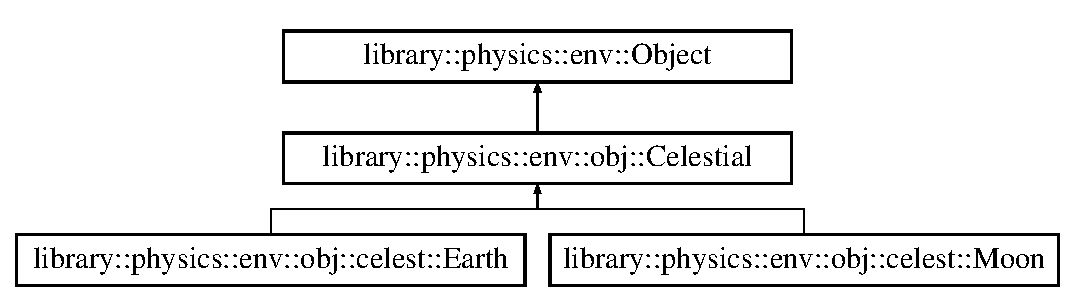
\includegraphics[height=2.403433cm]{classlibrary_1_1physics_1_1env_1_1obj_1_1_celestial}
\end{center}
\end{figure}
\subsection*{Classes}
\begin{DoxyCompactItemize}
\item 
struct \hyperlink{structlibrary_1_1physics_1_1env_1_1obj_1_1_celestial_1_1_model_base}{Model\+Base}
\end{DoxyCompactItemize}
\subsection*{Public Types}
\begin{DoxyCompactItemize}
\item 
enum \hyperlink{classlibrary_1_1physics_1_1env_1_1obj_1_1_celestial_aab1f58aa727e639288d65f3d33c4f245}{Type} \{ \newline
\hyperlink{classlibrary_1_1physics_1_1env_1_1obj_1_1_celestial_aab1f58aa727e639288d65f3d33c4f245aec0fc0100c4fc1ce4eea230c3dc10360}{Type\+::\+Undefined}, 
\hyperlink{classlibrary_1_1physics_1_1env_1_1obj_1_1_celestial_aab1f58aa727e639288d65f3d33c4f245aef6572e4cd58bb39a3f4e82fc64fe9f0}{Type\+::\+Sun}, 
\hyperlink{classlibrary_1_1physics_1_1env_1_1obj_1_1_celestial_aab1f58aa727e639288d65f3d33c4f245a34dae487e31f37aa74633258b7774d4f}{Type\+::\+Mercury}, 
\hyperlink{classlibrary_1_1physics_1_1env_1_1obj_1_1_celestial_aab1f58aa727e639288d65f3d33c4f245a0bdc508a17811a3a860d32749ad44e4b}{Type\+::\+Venus}, 
\newline
\hyperlink{classlibrary_1_1physics_1_1env_1_1obj_1_1_celestial_aab1f58aa727e639288d65f3d33c4f245a5cdd21c97f86686cc505e02fd32a7523}{Type\+::\+Earth}, 
\hyperlink{classlibrary_1_1physics_1_1env_1_1obj_1_1_celestial_aab1f58aa727e639288d65f3d33c4f245ad502a50ed945d5fca74e0105575b5b34}{Type\+::\+Moon}, 
\hyperlink{classlibrary_1_1physics_1_1env_1_1obj_1_1_celestial_aab1f58aa727e639288d65f3d33c4f245a671f028142280b556a85ffdd90e0a43d}{Type\+::\+Mars}
 \}
\item 
enum \hyperlink{classlibrary_1_1physics_1_1env_1_1obj_1_1_celestial_a8585fb32125cb6c73ae1339a5ea09c79}{Frame\+Type} \{ \hyperlink{classlibrary_1_1physics_1_1env_1_1obj_1_1_celestial_a8585fb32125cb6c73ae1339a5ea09c79aec0fc0100c4fc1ce4eea230c3dc10360}{Frame\+Type\+::\+Undefined}, 
\hyperlink{classlibrary_1_1physics_1_1env_1_1obj_1_1_celestial_a8585fb32125cb6c73ae1339a5ea09c79acd3459b28418fa8fa75ffaba4f3e7c74}{Frame\+Type\+::\+N\+ED}
 \}
\end{DoxyCompactItemize}
\subsection*{Public Member Functions}
\begin{DoxyCompactItemize}
\item 
\hyperlink{classlibrary_1_1physics_1_1env_1_1obj_1_1_celestial_ae3710304fcb39c6cee0b0f1b9ea646f1}{Celestial} (const String \&a\+Name, const \hyperlink{classlibrary_1_1physics_1_1env_1_1obj_1_1_celestial_aab1f58aa727e639288d65f3d33c4f245}{Celestial\+::\+Type} \&a\+Type, const \hyperlink{classlibrary_1_1physics_1_1units_1_1_derived}{Derived} \&a\+Gravitational\+Parameter, const \hyperlink{classlibrary_1_1physics_1_1units_1_1_length}{Length} \&an\+Equatorial\+Radius, const Real \&a\+Flattening, const Real \&a\+J2, const Shared$<$ \hyperlink{classlibrary_1_1physics_1_1env_1_1_ephemeris}{Ephemeris} $>$ \&an\+Ephemeris, const Shared$<$ \hyperlink{namespacelibrary_1_1physics_1_1env_1_1obj_ade509c84a4970a3420c03c058ada152a}{Gravitational\+Model} $>$ \&a\+Gravitational\+Model, const \hyperlink{classlibrary_1_1physics_1_1time_1_1_instant}{Instant} \&an\+Instant)
\item 
\hyperlink{classlibrary_1_1physics_1_1env_1_1obj_1_1_celestial_a7c2263420e3ebdb99523a87716f7575a}{Celestial} (const String \&a\+Name, const \hyperlink{classlibrary_1_1physics_1_1env_1_1obj_1_1_celestial_aab1f58aa727e639288d65f3d33c4f245}{Celestial\+::\+Type} \&a\+Type, const \hyperlink{classlibrary_1_1physics_1_1units_1_1_derived}{Derived} \&a\+Gravitational\+Parameter, const \hyperlink{classlibrary_1_1physics_1_1units_1_1_length}{Length} \&an\+Equatorial\+Radius, const Real \&a\+Flattening, const Real \&a\+J2, const Shared$<$ \hyperlink{classlibrary_1_1physics_1_1env_1_1_ephemeris}{Ephemeris} $>$ \&an\+Ephemeris, const Shared$<$ \hyperlink{namespacelibrary_1_1physics_1_1env_1_1obj_ade509c84a4970a3420c03c058ada152a}{Gravitational\+Model} $>$ \&a\+Gravitational\+Model, const \hyperlink{classlibrary_1_1physics_1_1time_1_1_instant}{Instant} \&an\+Instant, const \hyperlink{classlibrary_1_1physics_1_1env_1_1_object_abdf50733c7ad97327fb64edca5670f13}{Object\+::\+Geometry} \&a\+Geometry)
\item 
virtual \hyperlink{classlibrary_1_1physics_1_1env_1_1obj_1_1_celestial_a508a59c34ac23a582f2fed6003c4c907}{$\sim$\+Celestial} () override
\item 
virtual \hyperlink{classlibrary_1_1physics_1_1env_1_1obj_1_1_celestial}{Celestial} $\ast$ \hyperlink{classlibrary_1_1physics_1_1env_1_1obj_1_1_celestial_aaf8aa41a0ff9336eba62c07e3c27f82d}{clone} () const override
\item 
virtual bool \hyperlink{classlibrary_1_1physics_1_1env_1_1obj_1_1_celestial_a2b16a76f609891450356457de13c26d8}{is\+Defined} () const override
\item 
Shared$<$ const \hyperlink{classlibrary_1_1physics_1_1env_1_1_ephemeris}{Ephemeris} $>$ \hyperlink{classlibrary_1_1physics_1_1env_1_1obj_1_1_celestial_ab56fff3f2f1508dee79fa7410d67e300}{access\+Ephemeris} () const
\item 
Shared$<$ const \hyperlink{namespacelibrary_1_1physics_1_1env_1_1obj_ade509c84a4970a3420c03c058ada152a}{Gravitational\+Model} $>$ \hyperlink{classlibrary_1_1physics_1_1env_1_1obj_1_1_celestial_acbb834f37fa8f0fc7868d41ebb5173ee}{access\+Gravitational\+Model} () const
\item 
\hyperlink{classlibrary_1_1physics_1_1env_1_1obj_1_1_celestial_aab1f58aa727e639288d65f3d33c4f245}{Celestial\+::\+Type} \hyperlink{classlibrary_1_1physics_1_1env_1_1obj_1_1_celestial_ae020ad574249ea82679347c0a6933355}{get\+Type} () const
\item 
\hyperlink{classlibrary_1_1physics_1_1units_1_1_derived}{Derived} \hyperlink{classlibrary_1_1physics_1_1env_1_1obj_1_1_celestial_a2e8341c35d9c4c07eed4ce9aa5d9acc2}{get\+Gravitational\+Parameter} () const
\item 
\hyperlink{classlibrary_1_1physics_1_1units_1_1_length}{Length} \hyperlink{classlibrary_1_1physics_1_1env_1_1obj_1_1_celestial_a7dd4326ff317292262d1a9adf8887cfe}{get\+Equatorial\+Radius} () const
\item 
Real \hyperlink{classlibrary_1_1physics_1_1env_1_1obj_1_1_celestial_aac48ed47a25a10c120f066995dc3c6d4}{get\+Flattening} () const
\item 
Real \hyperlink{classlibrary_1_1physics_1_1env_1_1obj_1_1_celestial_a3740b398dca520bd50862f67c29ab8e7}{get\+J2} () const
\item 
virtual Shared$<$ const \hyperlink{classlibrary_1_1physics_1_1coord_1_1_frame}{Frame} $>$ \hyperlink{classlibrary_1_1physics_1_1env_1_1obj_1_1_celestial_a6649bfe0bf0795aa4def046a8c38aef5}{access\+Frame} () const override
\item 
virtual \hyperlink{classlibrary_1_1physics_1_1coord_1_1_position}{Position} \hyperlink{classlibrary_1_1physics_1_1env_1_1obj_1_1_celestial_aa2a209f37414e24303c21d994396664f}{get\+Position\+In} (const Shared$<$ const \hyperlink{classlibrary_1_1physics_1_1coord_1_1_frame}{Frame} $>$ \&a\+Frame\+S\+Ptr) const override
\item 
virtual \hyperlink{classlibrary_1_1physics_1_1coord_1_1_velocity}{Velocity} \hyperlink{classlibrary_1_1physics_1_1env_1_1obj_1_1_celestial_accaa3b1fdc39a1a058fd35006f31982d}{get\+Velocity\+In} (const Shared$<$ const \hyperlink{classlibrary_1_1physics_1_1coord_1_1_frame}{Frame} $>$ \&a\+Frame\+S\+Ptr) const override
\item 
virtual \hyperlink{classlibrary_1_1physics_1_1coord_1_1_transform}{Transform} \hyperlink{classlibrary_1_1physics_1_1env_1_1obj_1_1_celestial_ac6676b10ebbb63a8483137c9c734c58a}{get\+Transform\+To} (const Shared$<$ const \hyperlink{classlibrary_1_1physics_1_1coord_1_1_frame}{Frame} $>$ \&a\+Frame\+S\+Ptr) const override
\item 
virtual \hyperlink{classlibrary_1_1physics_1_1coord_1_1_axes}{Axes} \hyperlink{classlibrary_1_1physics_1_1env_1_1obj_1_1_celestial_a51d7ed3c0dcf627fbbcd81f9b190fb6b}{get\+Axes\+In} (const Shared$<$ const \hyperlink{classlibrary_1_1physics_1_1coord_1_1_frame}{Frame} $>$ \&a\+Frame\+S\+Ptr) const override
\item 
\hyperlink{classlibrary_1_1physics_1_1data_1_1_vector}{Vector} \hyperlink{classlibrary_1_1physics_1_1env_1_1obj_1_1_celestial_aa6313086a85ad19128d16f376a32aefe}{get\+Gravitational\+Field\+At} (const \hyperlink{classlibrary_1_1physics_1_1coord_1_1_position}{Position} \&a\+Position) const
\item 
Shared$<$ const \hyperlink{classlibrary_1_1physics_1_1coord_1_1_frame}{Frame} $>$ \hyperlink{classlibrary_1_1physics_1_1env_1_1obj_1_1_celestial_ad1dfffd88b216eccf83a9441cae304be}{get\+Frame\+At} (const \hyperlink{classlibrary_1_1physics_1_1coord_1_1spherical_1_1_l_l_a}{L\+LA} \&a\+Lla, const \hyperlink{classlibrary_1_1physics_1_1env_1_1obj_1_1_celestial_a8585fb32125cb6c73ae1339a5ea09c79}{Celestial\+::\+Frame\+Type} \&a\+Frame\+Type) const
\item 
\hyperlink{classlibrary_1_1physics_1_1env_1_1_object_abdf50733c7ad97327fb64edca5670f13}{Object\+::\+Geometry} \hyperlink{classlibrary_1_1physics_1_1env_1_1obj_1_1_celestial_aa910ed14605693ee5af68d88015cd53b}{get\+Terminator\+Geometry} () const
\end{DoxyCompactItemize}
\subsection*{Static Public Member Functions}
\begin{DoxyCompactItemize}
\item 
static \hyperlink{classlibrary_1_1physics_1_1env_1_1obj_1_1_celestial}{Celestial} \hyperlink{classlibrary_1_1physics_1_1env_1_1obj_1_1_celestial_a5e33230d05d77f5e1132151ecf5e94e9}{Undefined} ()
\item 
static String \hyperlink{classlibrary_1_1physics_1_1env_1_1obj_1_1_celestial_a020864aa551a1ec6f5674cc2e166b131}{String\+From\+Frame\+Type} (const \hyperlink{classlibrary_1_1physics_1_1env_1_1obj_1_1_celestial_a8585fb32125cb6c73ae1339a5ea09c79}{Celestial\+::\+Frame\+Type} \&a\+Frame\+Type)
\end{DoxyCompactItemize}


\subsection{Member Enumeration Documentation}
\mbox{\Hypertarget{classlibrary_1_1physics_1_1env_1_1obj_1_1_celestial_a8585fb32125cb6c73ae1339a5ea09c79}\label{classlibrary_1_1physics_1_1env_1_1obj_1_1_celestial_a8585fb32125cb6c73ae1339a5ea09c79}} 
\index{library\+::physics\+::env\+::obj\+::\+Celestial@{library\+::physics\+::env\+::obj\+::\+Celestial}!Frame\+Type@{Frame\+Type}}
\index{Frame\+Type@{Frame\+Type}!library\+::physics\+::env\+::obj\+::\+Celestial@{library\+::physics\+::env\+::obj\+::\+Celestial}}
\subsubsection{\texorpdfstring{Frame\+Type}{FrameType}}
{\footnotesize\ttfamily enum \hyperlink{classlibrary_1_1physics_1_1env_1_1obj_1_1_celestial_a8585fb32125cb6c73ae1339a5ea09c79}{library\+::physics\+::env\+::obj\+::\+Celestial\+::\+Frame\+Type}\hspace{0.3cm}{\ttfamily [strong]}}

\begin{DoxyEnumFields}{Enumerator}
\raisebox{\heightof{T}}[0pt][0pt]{\index{Undefined@{Undefined}!library\+::physics\+::env\+::obj\+::\+Celestial@{library\+::physics\+::env\+::obj\+::\+Celestial}}\index{library\+::physics\+::env\+::obj\+::\+Celestial@{library\+::physics\+::env\+::obj\+::\+Celestial}!Undefined@{Undefined}}}\mbox{\Hypertarget{classlibrary_1_1physics_1_1env_1_1obj_1_1_celestial_a8585fb32125cb6c73ae1339a5ea09c79aec0fc0100c4fc1ce4eea230c3dc10360}\label{classlibrary_1_1physics_1_1env_1_1obj_1_1_celestial_a8585fb32125cb6c73ae1339a5ea09c79aec0fc0100c4fc1ce4eea230c3dc10360}} 
Undefined&Undefined frame. \\
\hline

\raisebox{\heightof{T}}[0pt][0pt]{\index{N\+ED@{N\+ED}!library\+::physics\+::env\+::obj\+::\+Celestial@{library\+::physics\+::env\+::obj\+::\+Celestial}}\index{library\+::physics\+::env\+::obj\+::\+Celestial@{library\+::physics\+::env\+::obj\+::\+Celestial}!N\+ED@{N\+ED}}}\mbox{\Hypertarget{classlibrary_1_1physics_1_1env_1_1obj_1_1_celestial_a8585fb32125cb6c73ae1339a5ea09c79acd3459b28418fa8fa75ffaba4f3e7c74}\label{classlibrary_1_1physics_1_1env_1_1obj_1_1_celestial_a8585fb32125cb6c73ae1339a5ea09c79acd3459b28418fa8fa75ffaba4f3e7c74}} 
N\+ED&North-\/\+East-\/\+Down (N\+ED) frame. \\
\hline

\end{DoxyEnumFields}
\mbox{\Hypertarget{classlibrary_1_1physics_1_1env_1_1obj_1_1_celestial_aab1f58aa727e639288d65f3d33c4f245}\label{classlibrary_1_1physics_1_1env_1_1obj_1_1_celestial_aab1f58aa727e639288d65f3d33c4f245}} 
\index{library\+::physics\+::env\+::obj\+::\+Celestial@{library\+::physics\+::env\+::obj\+::\+Celestial}!Type@{Type}}
\index{Type@{Type}!library\+::physics\+::env\+::obj\+::\+Celestial@{library\+::physics\+::env\+::obj\+::\+Celestial}}
\subsubsection{\texorpdfstring{Type}{Type}}
{\footnotesize\ttfamily enum \hyperlink{classlibrary_1_1physics_1_1env_1_1obj_1_1_celestial_aab1f58aa727e639288d65f3d33c4f245}{library\+::physics\+::env\+::obj\+::\+Celestial\+::\+Type}\hspace{0.3cm}{\ttfamily [strong]}}

\begin{DoxyEnumFields}{Enumerator}
\raisebox{\heightof{T}}[0pt][0pt]{\index{Undefined@{Undefined}!library\+::physics\+::env\+::obj\+::\+Celestial@{library\+::physics\+::env\+::obj\+::\+Celestial}}\index{library\+::physics\+::env\+::obj\+::\+Celestial@{library\+::physics\+::env\+::obj\+::\+Celestial}!Undefined@{Undefined}}}\mbox{\Hypertarget{classlibrary_1_1physics_1_1env_1_1obj_1_1_celestial_aab1f58aa727e639288d65f3d33c4f245aec0fc0100c4fc1ce4eea230c3dc10360}\label{classlibrary_1_1physics_1_1env_1_1obj_1_1_celestial_aab1f58aa727e639288d65f3d33c4f245aec0fc0100c4fc1ce4eea230c3dc10360}} 
Undefined&\\
\hline

\raisebox{\heightof{T}}[0pt][0pt]{\index{Sun@{Sun}!library\+::physics\+::env\+::obj\+::\+Celestial@{library\+::physics\+::env\+::obj\+::\+Celestial}}\index{library\+::physics\+::env\+::obj\+::\+Celestial@{library\+::physics\+::env\+::obj\+::\+Celestial}!Sun@{Sun}}}\mbox{\Hypertarget{classlibrary_1_1physics_1_1env_1_1obj_1_1_celestial_aab1f58aa727e639288d65f3d33c4f245aef6572e4cd58bb39a3f4e82fc64fe9f0}\label{classlibrary_1_1physics_1_1env_1_1obj_1_1_celestial_aab1f58aa727e639288d65f3d33c4f245aef6572e4cd58bb39a3f4e82fc64fe9f0}} 
Sun&\\
\hline

\raisebox{\heightof{T}}[0pt][0pt]{\index{Mercury@{Mercury}!library\+::physics\+::env\+::obj\+::\+Celestial@{library\+::physics\+::env\+::obj\+::\+Celestial}}\index{library\+::physics\+::env\+::obj\+::\+Celestial@{library\+::physics\+::env\+::obj\+::\+Celestial}!Mercury@{Mercury}}}\mbox{\Hypertarget{classlibrary_1_1physics_1_1env_1_1obj_1_1_celestial_aab1f58aa727e639288d65f3d33c4f245a34dae487e31f37aa74633258b7774d4f}\label{classlibrary_1_1physics_1_1env_1_1obj_1_1_celestial_aab1f58aa727e639288d65f3d33c4f245a34dae487e31f37aa74633258b7774d4f}} 
Mercury&\\
\hline

\raisebox{\heightof{T}}[0pt][0pt]{\index{Venus@{Venus}!library\+::physics\+::env\+::obj\+::\+Celestial@{library\+::physics\+::env\+::obj\+::\+Celestial}}\index{library\+::physics\+::env\+::obj\+::\+Celestial@{library\+::physics\+::env\+::obj\+::\+Celestial}!Venus@{Venus}}}\mbox{\Hypertarget{classlibrary_1_1physics_1_1env_1_1obj_1_1_celestial_aab1f58aa727e639288d65f3d33c4f245a0bdc508a17811a3a860d32749ad44e4b}\label{classlibrary_1_1physics_1_1env_1_1obj_1_1_celestial_aab1f58aa727e639288d65f3d33c4f245a0bdc508a17811a3a860d32749ad44e4b}} 
Venus&\\
\hline

\raisebox{\heightof{T}}[0pt][0pt]{\index{Earth@{Earth}!library\+::physics\+::env\+::obj\+::\+Celestial@{library\+::physics\+::env\+::obj\+::\+Celestial}}\index{library\+::physics\+::env\+::obj\+::\+Celestial@{library\+::physics\+::env\+::obj\+::\+Celestial}!Earth@{Earth}}}\mbox{\Hypertarget{classlibrary_1_1physics_1_1env_1_1obj_1_1_celestial_aab1f58aa727e639288d65f3d33c4f245a5cdd21c97f86686cc505e02fd32a7523}\label{classlibrary_1_1physics_1_1env_1_1obj_1_1_celestial_aab1f58aa727e639288d65f3d33c4f245a5cdd21c97f86686cc505e02fd32a7523}} 
Earth&\\
\hline

\raisebox{\heightof{T}}[0pt][0pt]{\index{Moon@{Moon}!library\+::physics\+::env\+::obj\+::\+Celestial@{library\+::physics\+::env\+::obj\+::\+Celestial}}\index{library\+::physics\+::env\+::obj\+::\+Celestial@{library\+::physics\+::env\+::obj\+::\+Celestial}!Moon@{Moon}}}\mbox{\Hypertarget{classlibrary_1_1physics_1_1env_1_1obj_1_1_celestial_aab1f58aa727e639288d65f3d33c4f245ad502a50ed945d5fca74e0105575b5b34}\label{classlibrary_1_1physics_1_1env_1_1obj_1_1_celestial_aab1f58aa727e639288d65f3d33c4f245ad502a50ed945d5fca74e0105575b5b34}} 
Moon&\\
\hline

\raisebox{\heightof{T}}[0pt][0pt]{\index{Mars@{Mars}!library\+::physics\+::env\+::obj\+::\+Celestial@{library\+::physics\+::env\+::obj\+::\+Celestial}}\index{library\+::physics\+::env\+::obj\+::\+Celestial@{library\+::physics\+::env\+::obj\+::\+Celestial}!Mars@{Mars}}}\mbox{\Hypertarget{classlibrary_1_1physics_1_1env_1_1obj_1_1_celestial_aab1f58aa727e639288d65f3d33c4f245a671f028142280b556a85ffdd90e0a43d}\label{classlibrary_1_1physics_1_1env_1_1obj_1_1_celestial_aab1f58aa727e639288d65f3d33c4f245a671f028142280b556a85ffdd90e0a43d}} 
Mars&\\
\hline

\end{DoxyEnumFields}


\subsection{Constructor \& Destructor Documentation}
\mbox{\Hypertarget{classlibrary_1_1physics_1_1env_1_1obj_1_1_celestial_ae3710304fcb39c6cee0b0f1b9ea646f1}\label{classlibrary_1_1physics_1_1env_1_1obj_1_1_celestial_ae3710304fcb39c6cee0b0f1b9ea646f1}} 
\index{library\+::physics\+::env\+::obj\+::\+Celestial@{library\+::physics\+::env\+::obj\+::\+Celestial}!Celestial@{Celestial}}
\index{Celestial@{Celestial}!library\+::physics\+::env\+::obj\+::\+Celestial@{library\+::physics\+::env\+::obj\+::\+Celestial}}
\subsubsection{\texorpdfstring{Celestial()}{Celestial()}\hspace{0.1cm}{\footnotesize\ttfamily [1/2]}}
{\footnotesize\ttfamily library\+::physics\+::env\+::obj\+::\+Celestial\+::\+Celestial (\begin{DoxyParamCaption}\item[{const String \&}]{a\+Name,  }\item[{const \hyperlink{classlibrary_1_1physics_1_1env_1_1obj_1_1_celestial_aab1f58aa727e639288d65f3d33c4f245}{Celestial\+::\+Type} \&}]{a\+Type,  }\item[{const \hyperlink{classlibrary_1_1physics_1_1units_1_1_derived}{Derived} \&}]{a\+Gravitational\+Parameter,  }\item[{const \hyperlink{classlibrary_1_1physics_1_1units_1_1_length}{Length} \&}]{an\+Equatorial\+Radius,  }\item[{const Real \&}]{a\+Flattening,  }\item[{const Real \&}]{a\+J2,  }\item[{const Shared$<$ \hyperlink{classlibrary_1_1physics_1_1env_1_1_ephemeris}{Ephemeris} $>$ \&}]{an\+Ephemeris,  }\item[{const Shared$<$ \hyperlink{namespacelibrary_1_1physics_1_1env_1_1obj_ade509c84a4970a3420c03c058ada152a}{Gravitational\+Model} $>$ \&}]{a\+Gravitational\+Model,  }\item[{const \hyperlink{classlibrary_1_1physics_1_1time_1_1_instant}{Instant} \&}]{an\+Instant }\end{DoxyParamCaption})}

\mbox{\Hypertarget{classlibrary_1_1physics_1_1env_1_1obj_1_1_celestial_a7c2263420e3ebdb99523a87716f7575a}\label{classlibrary_1_1physics_1_1env_1_1obj_1_1_celestial_a7c2263420e3ebdb99523a87716f7575a}} 
\index{library\+::physics\+::env\+::obj\+::\+Celestial@{library\+::physics\+::env\+::obj\+::\+Celestial}!Celestial@{Celestial}}
\index{Celestial@{Celestial}!library\+::physics\+::env\+::obj\+::\+Celestial@{library\+::physics\+::env\+::obj\+::\+Celestial}}
\subsubsection{\texorpdfstring{Celestial()}{Celestial()}\hspace{0.1cm}{\footnotesize\ttfamily [2/2]}}
{\footnotesize\ttfamily library\+::physics\+::env\+::obj\+::\+Celestial\+::\+Celestial (\begin{DoxyParamCaption}\item[{const String \&}]{a\+Name,  }\item[{const \hyperlink{classlibrary_1_1physics_1_1env_1_1obj_1_1_celestial_aab1f58aa727e639288d65f3d33c4f245}{Celestial\+::\+Type} \&}]{a\+Type,  }\item[{const \hyperlink{classlibrary_1_1physics_1_1units_1_1_derived}{Derived} \&}]{a\+Gravitational\+Parameter,  }\item[{const \hyperlink{classlibrary_1_1physics_1_1units_1_1_length}{Length} \&}]{an\+Equatorial\+Radius,  }\item[{const Real \&}]{a\+Flattening,  }\item[{const Real \&}]{a\+J2,  }\item[{const Shared$<$ \hyperlink{classlibrary_1_1physics_1_1env_1_1_ephemeris}{Ephemeris} $>$ \&}]{an\+Ephemeris,  }\item[{const Shared$<$ \hyperlink{namespacelibrary_1_1physics_1_1env_1_1obj_ade509c84a4970a3420c03c058ada152a}{Gravitational\+Model} $>$ \&}]{a\+Gravitational\+Model,  }\item[{const \hyperlink{classlibrary_1_1physics_1_1time_1_1_instant}{Instant} \&}]{an\+Instant,  }\item[{const \hyperlink{classlibrary_1_1physics_1_1env_1_1_object_abdf50733c7ad97327fb64edca5670f13}{Object\+::\+Geometry} \&}]{a\+Geometry }\end{DoxyParamCaption})}

\mbox{\Hypertarget{classlibrary_1_1physics_1_1env_1_1obj_1_1_celestial_a508a59c34ac23a582f2fed6003c4c907}\label{classlibrary_1_1physics_1_1env_1_1obj_1_1_celestial_a508a59c34ac23a582f2fed6003c4c907}} 
\index{library\+::physics\+::env\+::obj\+::\+Celestial@{library\+::physics\+::env\+::obj\+::\+Celestial}!````~Celestial@{$\sim$\+Celestial}}
\index{````~Celestial@{$\sim$\+Celestial}!library\+::physics\+::env\+::obj\+::\+Celestial@{library\+::physics\+::env\+::obj\+::\+Celestial}}
\subsubsection{\texorpdfstring{$\sim$\+Celestial()}{~Celestial()}}
{\footnotesize\ttfamily library\+::physics\+::env\+::obj\+::\+Celestial\+::$\sim$\+Celestial (\begin{DoxyParamCaption}{ }\end{DoxyParamCaption})\hspace{0.3cm}{\ttfamily [override]}, {\ttfamily [virtual]}}



\subsection{Member Function Documentation}
\mbox{\Hypertarget{classlibrary_1_1physics_1_1env_1_1obj_1_1_celestial_ab56fff3f2f1508dee79fa7410d67e300}\label{classlibrary_1_1physics_1_1env_1_1obj_1_1_celestial_ab56fff3f2f1508dee79fa7410d67e300}} 
\index{library\+::physics\+::env\+::obj\+::\+Celestial@{library\+::physics\+::env\+::obj\+::\+Celestial}!access\+Ephemeris@{access\+Ephemeris}}
\index{access\+Ephemeris@{access\+Ephemeris}!library\+::physics\+::env\+::obj\+::\+Celestial@{library\+::physics\+::env\+::obj\+::\+Celestial}}
\subsubsection{\texorpdfstring{access\+Ephemeris()}{accessEphemeris()}}
{\footnotesize\ttfamily Shared$<$ const \hyperlink{classlibrary_1_1physics_1_1env_1_1_ephemeris}{Ephemeris} $>$ library\+::physics\+::env\+::obj\+::\+Celestial\+::access\+Ephemeris (\begin{DoxyParamCaption}{ }\end{DoxyParamCaption}) const}

\mbox{\Hypertarget{classlibrary_1_1physics_1_1env_1_1obj_1_1_celestial_a6649bfe0bf0795aa4def046a8c38aef5}\label{classlibrary_1_1physics_1_1env_1_1obj_1_1_celestial_a6649bfe0bf0795aa4def046a8c38aef5}} 
\index{library\+::physics\+::env\+::obj\+::\+Celestial@{library\+::physics\+::env\+::obj\+::\+Celestial}!access\+Frame@{access\+Frame}}
\index{access\+Frame@{access\+Frame}!library\+::physics\+::env\+::obj\+::\+Celestial@{library\+::physics\+::env\+::obj\+::\+Celestial}}
\subsubsection{\texorpdfstring{access\+Frame()}{accessFrame()}}
{\footnotesize\ttfamily Shared$<$ const \hyperlink{classlibrary_1_1physics_1_1coord_1_1_frame}{Frame} $>$ library\+::physics\+::env\+::obj\+::\+Celestial\+::access\+Frame (\begin{DoxyParamCaption}{ }\end{DoxyParamCaption}) const\hspace{0.3cm}{\ttfamily [override]}, {\ttfamily [virtual]}}



Implements \hyperlink{classlibrary_1_1physics_1_1env_1_1_object_a6ff59bc7375388118c60b5823dad748b}{library\+::physics\+::env\+::\+Object}.

\mbox{\Hypertarget{classlibrary_1_1physics_1_1env_1_1obj_1_1_celestial_acbb834f37fa8f0fc7868d41ebb5173ee}\label{classlibrary_1_1physics_1_1env_1_1obj_1_1_celestial_acbb834f37fa8f0fc7868d41ebb5173ee}} 
\index{library\+::physics\+::env\+::obj\+::\+Celestial@{library\+::physics\+::env\+::obj\+::\+Celestial}!access\+Gravitational\+Model@{access\+Gravitational\+Model}}
\index{access\+Gravitational\+Model@{access\+Gravitational\+Model}!library\+::physics\+::env\+::obj\+::\+Celestial@{library\+::physics\+::env\+::obj\+::\+Celestial}}
\subsubsection{\texorpdfstring{access\+Gravitational\+Model()}{accessGravitationalModel()}}
{\footnotesize\ttfamily Shared$<$ const \hyperlink{namespacelibrary_1_1physics_1_1env_1_1obj_ade509c84a4970a3420c03c058ada152a}{Gravitational\+Model} $>$ library\+::physics\+::env\+::obj\+::\+Celestial\+::access\+Gravitational\+Model (\begin{DoxyParamCaption}{ }\end{DoxyParamCaption}) const}

\mbox{\Hypertarget{classlibrary_1_1physics_1_1env_1_1obj_1_1_celestial_aaf8aa41a0ff9336eba62c07e3c27f82d}\label{classlibrary_1_1physics_1_1env_1_1obj_1_1_celestial_aaf8aa41a0ff9336eba62c07e3c27f82d}} 
\index{library\+::physics\+::env\+::obj\+::\+Celestial@{library\+::physics\+::env\+::obj\+::\+Celestial}!clone@{clone}}
\index{clone@{clone}!library\+::physics\+::env\+::obj\+::\+Celestial@{library\+::physics\+::env\+::obj\+::\+Celestial}}
\subsubsection{\texorpdfstring{clone()}{clone()}}
{\footnotesize\ttfamily \hyperlink{classlibrary_1_1physics_1_1env_1_1obj_1_1_celestial}{Celestial} $\ast$ library\+::physics\+::env\+::obj\+::\+Celestial\+::clone (\begin{DoxyParamCaption}{ }\end{DoxyParamCaption}) const\hspace{0.3cm}{\ttfamily [override]}, {\ttfamily [virtual]}}



Implements \hyperlink{classlibrary_1_1physics_1_1env_1_1_object_a498e0d1a15e937a5aa77374c6f899768}{library\+::physics\+::env\+::\+Object}.



Reimplemented in \hyperlink{classlibrary_1_1physics_1_1env_1_1obj_1_1celest_1_1_earth_aca39bec00a2046a3fcef9bf22be52428}{library\+::physics\+::env\+::obj\+::celest\+::\+Earth}, \hyperlink{classlibrary_1_1physics_1_1env_1_1obj_1_1celest_1_1_moon_a9d922ab338809a6c1052edbe11ce3e60}{library\+::physics\+::env\+::obj\+::celest\+::\+Moon}, and \hyperlink{classlibrary_1_1physics_1_1env_1_1obj_1_1celest_1_1_sun_a79fa2d336dad399c3d933b0f5a2f9427}{library\+::physics\+::env\+::obj\+::celest\+::\+Sun}.

\mbox{\Hypertarget{classlibrary_1_1physics_1_1env_1_1obj_1_1_celestial_a51d7ed3c0dcf627fbbcd81f9b190fb6b}\label{classlibrary_1_1physics_1_1env_1_1obj_1_1_celestial_a51d7ed3c0dcf627fbbcd81f9b190fb6b}} 
\index{library\+::physics\+::env\+::obj\+::\+Celestial@{library\+::physics\+::env\+::obj\+::\+Celestial}!get\+Axes\+In@{get\+Axes\+In}}
\index{get\+Axes\+In@{get\+Axes\+In}!library\+::physics\+::env\+::obj\+::\+Celestial@{library\+::physics\+::env\+::obj\+::\+Celestial}}
\subsubsection{\texorpdfstring{get\+Axes\+In()}{getAxesIn()}}
{\footnotesize\ttfamily \hyperlink{classlibrary_1_1physics_1_1coord_1_1_axes}{Axes} library\+::physics\+::env\+::obj\+::\+Celestial\+::get\+Axes\+In (\begin{DoxyParamCaption}\item[{const Shared$<$ const \hyperlink{classlibrary_1_1physics_1_1coord_1_1_frame}{Frame} $>$ \&}]{a\+Frame\+S\+Ptr }\end{DoxyParamCaption}) const\hspace{0.3cm}{\ttfamily [override]}, {\ttfamily [virtual]}}



Implements \hyperlink{classlibrary_1_1physics_1_1env_1_1_object_a6807199a92fd78c10c6327b9ca654f50}{library\+::physics\+::env\+::\+Object}.

\mbox{\Hypertarget{classlibrary_1_1physics_1_1env_1_1obj_1_1_celestial_a7dd4326ff317292262d1a9adf8887cfe}\label{classlibrary_1_1physics_1_1env_1_1obj_1_1_celestial_a7dd4326ff317292262d1a9adf8887cfe}} 
\index{library\+::physics\+::env\+::obj\+::\+Celestial@{library\+::physics\+::env\+::obj\+::\+Celestial}!get\+Equatorial\+Radius@{get\+Equatorial\+Radius}}
\index{get\+Equatorial\+Radius@{get\+Equatorial\+Radius}!library\+::physics\+::env\+::obj\+::\+Celestial@{library\+::physics\+::env\+::obj\+::\+Celestial}}
\subsubsection{\texorpdfstring{get\+Equatorial\+Radius()}{getEquatorialRadius()}}
{\footnotesize\ttfamily \hyperlink{classlibrary_1_1physics_1_1units_1_1_length}{Length} library\+::physics\+::env\+::obj\+::\+Celestial\+::get\+Equatorial\+Radius (\begin{DoxyParamCaption}{ }\end{DoxyParamCaption}) const}

\mbox{\Hypertarget{classlibrary_1_1physics_1_1env_1_1obj_1_1_celestial_aac48ed47a25a10c120f066995dc3c6d4}\label{classlibrary_1_1physics_1_1env_1_1obj_1_1_celestial_aac48ed47a25a10c120f066995dc3c6d4}} 
\index{library\+::physics\+::env\+::obj\+::\+Celestial@{library\+::physics\+::env\+::obj\+::\+Celestial}!get\+Flattening@{get\+Flattening}}
\index{get\+Flattening@{get\+Flattening}!library\+::physics\+::env\+::obj\+::\+Celestial@{library\+::physics\+::env\+::obj\+::\+Celestial}}
\subsubsection{\texorpdfstring{get\+Flattening()}{getFlattening()}}
{\footnotesize\ttfamily Real library\+::physics\+::env\+::obj\+::\+Celestial\+::get\+Flattening (\begin{DoxyParamCaption}{ }\end{DoxyParamCaption}) const}

\mbox{\Hypertarget{classlibrary_1_1physics_1_1env_1_1obj_1_1_celestial_ad1dfffd88b216eccf83a9441cae304be}\label{classlibrary_1_1physics_1_1env_1_1obj_1_1_celestial_ad1dfffd88b216eccf83a9441cae304be}} 
\index{library\+::physics\+::env\+::obj\+::\+Celestial@{library\+::physics\+::env\+::obj\+::\+Celestial}!get\+Frame\+At@{get\+Frame\+At}}
\index{get\+Frame\+At@{get\+Frame\+At}!library\+::physics\+::env\+::obj\+::\+Celestial@{library\+::physics\+::env\+::obj\+::\+Celestial}}
\subsubsection{\texorpdfstring{get\+Frame\+At()}{getFrameAt()}}
{\footnotesize\ttfamily Shared$<$ const \hyperlink{classlibrary_1_1physics_1_1coord_1_1_frame}{Frame} $>$ library\+::physics\+::env\+::obj\+::\+Celestial\+::get\+Frame\+At (\begin{DoxyParamCaption}\item[{const \hyperlink{classlibrary_1_1physics_1_1coord_1_1spherical_1_1_l_l_a}{L\+LA} \&}]{a\+Lla,  }\item[{const \hyperlink{classlibrary_1_1physics_1_1env_1_1obj_1_1_celestial_a8585fb32125cb6c73ae1339a5ea09c79}{Celestial\+::\+Frame\+Type} \&}]{a\+Frame\+Type }\end{DoxyParamCaption}) const}

\mbox{\Hypertarget{classlibrary_1_1physics_1_1env_1_1obj_1_1_celestial_aa6313086a85ad19128d16f376a32aefe}\label{classlibrary_1_1physics_1_1env_1_1obj_1_1_celestial_aa6313086a85ad19128d16f376a32aefe}} 
\index{library\+::physics\+::env\+::obj\+::\+Celestial@{library\+::physics\+::env\+::obj\+::\+Celestial}!get\+Gravitational\+Field\+At@{get\+Gravitational\+Field\+At}}
\index{get\+Gravitational\+Field\+At@{get\+Gravitational\+Field\+At}!library\+::physics\+::env\+::obj\+::\+Celestial@{library\+::physics\+::env\+::obj\+::\+Celestial}}
\subsubsection{\texorpdfstring{get\+Gravitational\+Field\+At()}{getGravitationalFieldAt()}}
{\footnotesize\ttfamily \hyperlink{classlibrary_1_1physics_1_1data_1_1_vector}{Vector} library\+::physics\+::env\+::obj\+::\+Celestial\+::get\+Gravitational\+Field\+At (\begin{DoxyParamCaption}\item[{const \hyperlink{classlibrary_1_1physics_1_1coord_1_1_position}{Position} \&}]{a\+Position }\end{DoxyParamCaption}) const}

\mbox{\Hypertarget{classlibrary_1_1physics_1_1env_1_1obj_1_1_celestial_a2e8341c35d9c4c07eed4ce9aa5d9acc2}\label{classlibrary_1_1physics_1_1env_1_1obj_1_1_celestial_a2e8341c35d9c4c07eed4ce9aa5d9acc2}} 
\index{library\+::physics\+::env\+::obj\+::\+Celestial@{library\+::physics\+::env\+::obj\+::\+Celestial}!get\+Gravitational\+Parameter@{get\+Gravitational\+Parameter}}
\index{get\+Gravitational\+Parameter@{get\+Gravitational\+Parameter}!library\+::physics\+::env\+::obj\+::\+Celestial@{library\+::physics\+::env\+::obj\+::\+Celestial}}
\subsubsection{\texorpdfstring{get\+Gravitational\+Parameter()}{getGravitationalParameter()}}
{\footnotesize\ttfamily \hyperlink{classlibrary_1_1physics_1_1units_1_1_derived}{Derived} library\+::physics\+::env\+::obj\+::\+Celestial\+::get\+Gravitational\+Parameter (\begin{DoxyParamCaption}{ }\end{DoxyParamCaption}) const}

\mbox{\Hypertarget{classlibrary_1_1physics_1_1env_1_1obj_1_1_celestial_a3740b398dca520bd50862f67c29ab8e7}\label{classlibrary_1_1physics_1_1env_1_1obj_1_1_celestial_a3740b398dca520bd50862f67c29ab8e7}} 
\index{library\+::physics\+::env\+::obj\+::\+Celestial@{library\+::physics\+::env\+::obj\+::\+Celestial}!get\+J2@{get\+J2}}
\index{get\+J2@{get\+J2}!library\+::physics\+::env\+::obj\+::\+Celestial@{library\+::physics\+::env\+::obj\+::\+Celestial}}
\subsubsection{\texorpdfstring{get\+J2()}{getJ2()}}
{\footnotesize\ttfamily Real library\+::physics\+::env\+::obj\+::\+Celestial\+::get\+J2 (\begin{DoxyParamCaption}{ }\end{DoxyParamCaption}) const}

\mbox{\Hypertarget{classlibrary_1_1physics_1_1env_1_1obj_1_1_celestial_aa2a209f37414e24303c21d994396664f}\label{classlibrary_1_1physics_1_1env_1_1obj_1_1_celestial_aa2a209f37414e24303c21d994396664f}} 
\index{library\+::physics\+::env\+::obj\+::\+Celestial@{library\+::physics\+::env\+::obj\+::\+Celestial}!get\+Position\+In@{get\+Position\+In}}
\index{get\+Position\+In@{get\+Position\+In}!library\+::physics\+::env\+::obj\+::\+Celestial@{library\+::physics\+::env\+::obj\+::\+Celestial}}
\subsubsection{\texorpdfstring{get\+Position\+In()}{getPositionIn()}}
{\footnotesize\ttfamily \hyperlink{classlibrary_1_1physics_1_1coord_1_1_position}{Position} library\+::physics\+::env\+::obj\+::\+Celestial\+::get\+Position\+In (\begin{DoxyParamCaption}\item[{const Shared$<$ const \hyperlink{classlibrary_1_1physics_1_1coord_1_1_frame}{Frame} $>$ \&}]{a\+Frame\+S\+Ptr }\end{DoxyParamCaption}) const\hspace{0.3cm}{\ttfamily [override]}, {\ttfamily [virtual]}}



Implements \hyperlink{classlibrary_1_1physics_1_1env_1_1_object_acc86d12ad94de870fc2684f7b768b617}{library\+::physics\+::env\+::\+Object}.

\mbox{\Hypertarget{classlibrary_1_1physics_1_1env_1_1obj_1_1_celestial_aa910ed14605693ee5af68d88015cd53b}\label{classlibrary_1_1physics_1_1env_1_1obj_1_1_celestial_aa910ed14605693ee5af68d88015cd53b}} 
\index{library\+::physics\+::env\+::obj\+::\+Celestial@{library\+::physics\+::env\+::obj\+::\+Celestial}!get\+Terminator\+Geometry@{get\+Terminator\+Geometry}}
\index{get\+Terminator\+Geometry@{get\+Terminator\+Geometry}!library\+::physics\+::env\+::obj\+::\+Celestial@{library\+::physics\+::env\+::obj\+::\+Celestial}}
\subsubsection{\texorpdfstring{get\+Terminator\+Geometry()}{getTerminatorGeometry()}}
{\footnotesize\ttfamily \hyperlink{classlibrary_1_1physics_1_1env_1_1_object_abdf50733c7ad97327fb64edca5670f13}{Object\+::\+Geometry} library\+::physics\+::env\+::obj\+::\+Celestial\+::get\+Terminator\+Geometry (\begin{DoxyParamCaption}{ }\end{DoxyParamCaption}) const}

\mbox{\Hypertarget{classlibrary_1_1physics_1_1env_1_1obj_1_1_celestial_ac6676b10ebbb63a8483137c9c734c58a}\label{classlibrary_1_1physics_1_1env_1_1obj_1_1_celestial_ac6676b10ebbb63a8483137c9c734c58a}} 
\index{library\+::physics\+::env\+::obj\+::\+Celestial@{library\+::physics\+::env\+::obj\+::\+Celestial}!get\+Transform\+To@{get\+Transform\+To}}
\index{get\+Transform\+To@{get\+Transform\+To}!library\+::physics\+::env\+::obj\+::\+Celestial@{library\+::physics\+::env\+::obj\+::\+Celestial}}
\subsubsection{\texorpdfstring{get\+Transform\+To()}{getTransformTo()}}
{\footnotesize\ttfamily \hyperlink{classlibrary_1_1physics_1_1coord_1_1_transform}{Transform} library\+::physics\+::env\+::obj\+::\+Celestial\+::get\+Transform\+To (\begin{DoxyParamCaption}\item[{const Shared$<$ const \hyperlink{classlibrary_1_1physics_1_1coord_1_1_frame}{Frame} $>$ \&}]{a\+Frame\+S\+Ptr }\end{DoxyParamCaption}) const\hspace{0.3cm}{\ttfamily [override]}, {\ttfamily [virtual]}}



Implements \hyperlink{classlibrary_1_1physics_1_1env_1_1_object_abe850e2334c19ae185456cd52aeeca7d}{library\+::physics\+::env\+::\+Object}.

\mbox{\Hypertarget{classlibrary_1_1physics_1_1env_1_1obj_1_1_celestial_ae020ad574249ea82679347c0a6933355}\label{classlibrary_1_1physics_1_1env_1_1obj_1_1_celestial_ae020ad574249ea82679347c0a6933355}} 
\index{library\+::physics\+::env\+::obj\+::\+Celestial@{library\+::physics\+::env\+::obj\+::\+Celestial}!get\+Type@{get\+Type}}
\index{get\+Type@{get\+Type}!library\+::physics\+::env\+::obj\+::\+Celestial@{library\+::physics\+::env\+::obj\+::\+Celestial}}
\subsubsection{\texorpdfstring{get\+Type()}{getType()}}
{\footnotesize\ttfamily \hyperlink{classlibrary_1_1physics_1_1env_1_1obj_1_1_celestial_aab1f58aa727e639288d65f3d33c4f245}{Celestial\+::\+Type} library\+::physics\+::env\+::obj\+::\+Celestial\+::get\+Type (\begin{DoxyParamCaption}{ }\end{DoxyParamCaption}) const}

\mbox{\Hypertarget{classlibrary_1_1physics_1_1env_1_1obj_1_1_celestial_accaa3b1fdc39a1a058fd35006f31982d}\label{classlibrary_1_1physics_1_1env_1_1obj_1_1_celestial_accaa3b1fdc39a1a058fd35006f31982d}} 
\index{library\+::physics\+::env\+::obj\+::\+Celestial@{library\+::physics\+::env\+::obj\+::\+Celestial}!get\+Velocity\+In@{get\+Velocity\+In}}
\index{get\+Velocity\+In@{get\+Velocity\+In}!library\+::physics\+::env\+::obj\+::\+Celestial@{library\+::physics\+::env\+::obj\+::\+Celestial}}
\subsubsection{\texorpdfstring{get\+Velocity\+In()}{getVelocityIn()}}
{\footnotesize\ttfamily \hyperlink{classlibrary_1_1physics_1_1coord_1_1_velocity}{Velocity} library\+::physics\+::env\+::obj\+::\+Celestial\+::get\+Velocity\+In (\begin{DoxyParamCaption}\item[{const Shared$<$ const \hyperlink{classlibrary_1_1physics_1_1coord_1_1_frame}{Frame} $>$ \&}]{a\+Frame\+S\+Ptr }\end{DoxyParamCaption}) const\hspace{0.3cm}{\ttfamily [override]}, {\ttfamily [virtual]}}



Implements \hyperlink{classlibrary_1_1physics_1_1env_1_1_object_a1a8f4358db37b1b8830866373f8f3670}{library\+::physics\+::env\+::\+Object}.

\mbox{\Hypertarget{classlibrary_1_1physics_1_1env_1_1obj_1_1_celestial_a2b16a76f609891450356457de13c26d8}\label{classlibrary_1_1physics_1_1env_1_1obj_1_1_celestial_a2b16a76f609891450356457de13c26d8}} 
\index{library\+::physics\+::env\+::obj\+::\+Celestial@{library\+::physics\+::env\+::obj\+::\+Celestial}!is\+Defined@{is\+Defined}}
\index{is\+Defined@{is\+Defined}!library\+::physics\+::env\+::obj\+::\+Celestial@{library\+::physics\+::env\+::obj\+::\+Celestial}}
\subsubsection{\texorpdfstring{is\+Defined()}{isDefined()}}
{\footnotesize\ttfamily bool library\+::physics\+::env\+::obj\+::\+Celestial\+::is\+Defined (\begin{DoxyParamCaption}{ }\end{DoxyParamCaption}) const\hspace{0.3cm}{\ttfamily [override]}, {\ttfamily [virtual]}}



Reimplemented from \hyperlink{classlibrary_1_1physics_1_1env_1_1_object_a7035edc921681401ddd43b094645a024}{library\+::physics\+::env\+::\+Object}.

\mbox{\Hypertarget{classlibrary_1_1physics_1_1env_1_1obj_1_1_celestial_a020864aa551a1ec6f5674cc2e166b131}\label{classlibrary_1_1physics_1_1env_1_1obj_1_1_celestial_a020864aa551a1ec6f5674cc2e166b131}} 
\index{library\+::physics\+::env\+::obj\+::\+Celestial@{library\+::physics\+::env\+::obj\+::\+Celestial}!String\+From\+Frame\+Type@{String\+From\+Frame\+Type}}
\index{String\+From\+Frame\+Type@{String\+From\+Frame\+Type}!library\+::physics\+::env\+::obj\+::\+Celestial@{library\+::physics\+::env\+::obj\+::\+Celestial}}
\subsubsection{\texorpdfstring{String\+From\+Frame\+Type()}{StringFromFrameType()}}
{\footnotesize\ttfamily String library\+::physics\+::env\+::obj\+::\+Celestial\+::\+String\+From\+Frame\+Type (\begin{DoxyParamCaption}\item[{const \hyperlink{classlibrary_1_1physics_1_1env_1_1obj_1_1_celestial_a8585fb32125cb6c73ae1339a5ea09c79}{Celestial\+::\+Frame\+Type} \&}]{a\+Frame\+Type }\end{DoxyParamCaption})\hspace{0.3cm}{\ttfamily [static]}}

\mbox{\Hypertarget{classlibrary_1_1physics_1_1env_1_1obj_1_1_celestial_a5e33230d05d77f5e1132151ecf5e94e9}\label{classlibrary_1_1physics_1_1env_1_1obj_1_1_celestial_a5e33230d05d77f5e1132151ecf5e94e9}} 
\index{library\+::physics\+::env\+::obj\+::\+Celestial@{library\+::physics\+::env\+::obj\+::\+Celestial}!Undefined@{Undefined}}
\index{Undefined@{Undefined}!library\+::physics\+::env\+::obj\+::\+Celestial@{library\+::physics\+::env\+::obj\+::\+Celestial}}
\subsubsection{\texorpdfstring{Undefined()}{Undefined()}}
{\footnotesize\ttfamily \hyperlink{classlibrary_1_1physics_1_1env_1_1obj_1_1_celestial}{Celestial} library\+::physics\+::env\+::obj\+::\+Celestial\+::\+Undefined (\begin{DoxyParamCaption}{ }\end{DoxyParamCaption})\hspace{0.3cm}{\ttfamily [static]}}



The documentation for this class was generated from the following files\+:\begin{DoxyCompactItemize}
\item 
include/\+Library/\+Physics/\+Environment/\+Objects/\hyperlink{_celestial_8hpp}{Celestial.\+hpp}\item 
src/\+Library/\+Physics/\+Environment/\+Objects/\hyperlink{_celestial_8cpp}{Celestial.\+cpp}\end{DoxyCompactItemize}

\hypertarget{classlibrary_1_1physics_1_1coord_1_1frame_1_1provider_1_1_c_i_r_f}{}\section{library\+:\+:physics\+:\+:coord\+:\+:frame\+:\+:provider\+:\+:C\+I\+RF Class Reference}
\label{classlibrary_1_1physics_1_1coord_1_1frame_1_1provider_1_1_c_i_r_f}\index{library\+::physics\+::coord\+::frame\+::provider\+::\+C\+I\+RF@{library\+::physics\+::coord\+::frame\+::provider\+::\+C\+I\+RF}}


Celestial Intermediate Reference \hyperlink{classlibrary_1_1physics_1_1coord_1_1_frame}{Frame} (\hyperlink{classlibrary_1_1physics_1_1coord_1_1frame_1_1provider_1_1_c_i_r_f}{C\+I\+RF}) provider.  




{\ttfamily \#include $<$C\+I\+R\+F.\+hpp$>$}

Inheritance diagram for library\+:\+:physics\+:\+:coord\+:\+:frame\+:\+:provider\+:\+:C\+I\+RF\+:\begin{figure}[H]
\begin{center}
\leavevmode
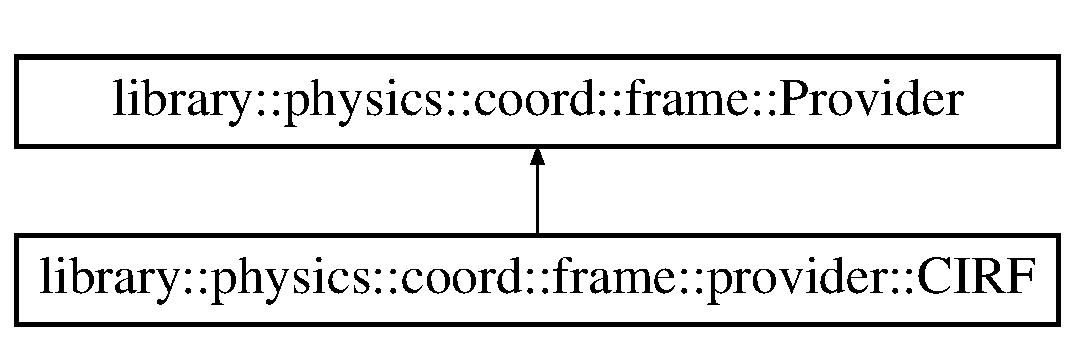
\includegraphics[height=2.000000cm]{classlibrary_1_1physics_1_1coord_1_1frame_1_1provider_1_1_c_i_r_f}
\end{center}
\end{figure}
\subsection*{Public Member Functions}
\begin{DoxyCompactItemize}
\item 
\hyperlink{classlibrary_1_1physics_1_1coord_1_1frame_1_1provider_1_1_c_i_r_f_a69759da2122df1ba03dc52f708b1cc8b}{C\+I\+RF} ()
\item 
virtual \hyperlink{classlibrary_1_1physics_1_1coord_1_1frame_1_1provider_1_1_c_i_r_f_aded0757cb9c4deab34318e65f74f05b8}{$\sim$\+C\+I\+RF} () override
\item 
virtual \hyperlink{classlibrary_1_1physics_1_1coord_1_1frame_1_1provider_1_1_c_i_r_f}{C\+I\+RF} $\ast$ \hyperlink{classlibrary_1_1physics_1_1coord_1_1frame_1_1provider_1_1_c_i_r_f_af75424e9e3a86a5aa06f998a8710c5c2}{clone} () const override
\item 
virtual bool \hyperlink{classlibrary_1_1physics_1_1coord_1_1frame_1_1provider_1_1_c_i_r_f_ab5676de1c31ad796d56a684615fabdf8}{is\+Defined} () const override
\item 
virtual \hyperlink{classlibrary_1_1physics_1_1coord_1_1_transform}{Transform} \hyperlink{classlibrary_1_1physics_1_1coord_1_1frame_1_1provider_1_1_c_i_r_f_afa16d0f890856396364443239ceac509}{get\+Transform\+At} (const \hyperlink{classlibrary_1_1physics_1_1time_1_1_instant}{Instant} \&an\+Instant) const override
\end{DoxyCompactItemize}


\subsection{Detailed Description}
Celestial Intermediate Reference \hyperlink{classlibrary_1_1physics_1_1coord_1_1_frame}{Frame} (\hyperlink{classlibrary_1_1physics_1_1coord_1_1frame_1_1provider_1_1_c_i_r_f}{C\+I\+RF}) provider. 

Bias, precession-\/nutation

https\+://www.iers.\+org/\+Shared\+Docs/\+Publikationen/\+E\+N/\+I\+E\+R\+S/\+Publications/tn/\+Techn\+Note36/tn36\+\_\+174.pdf?\+\_\+\+\_\+blob=publication\+File\&v=1 

\subsection{Constructor \& Destructor Documentation}
\mbox{\Hypertarget{classlibrary_1_1physics_1_1coord_1_1frame_1_1provider_1_1_c_i_r_f_a69759da2122df1ba03dc52f708b1cc8b}\label{classlibrary_1_1physics_1_1coord_1_1frame_1_1provider_1_1_c_i_r_f_a69759da2122df1ba03dc52f708b1cc8b}} 
\index{library\+::physics\+::coord\+::frame\+::provider\+::\+C\+I\+RF@{library\+::physics\+::coord\+::frame\+::provider\+::\+C\+I\+RF}!C\+I\+RF@{C\+I\+RF}}
\index{C\+I\+RF@{C\+I\+RF}!library\+::physics\+::coord\+::frame\+::provider\+::\+C\+I\+RF@{library\+::physics\+::coord\+::frame\+::provider\+::\+C\+I\+RF}}
\subsubsection{\texorpdfstring{C\+I\+R\+F()}{CIRF()}}
{\footnotesize\ttfamily library\+::physics\+::coord\+::frame\+::provider\+::\+C\+I\+R\+F\+::\+C\+I\+RF (\begin{DoxyParamCaption}{ }\end{DoxyParamCaption})}

\mbox{\Hypertarget{classlibrary_1_1physics_1_1coord_1_1frame_1_1provider_1_1_c_i_r_f_aded0757cb9c4deab34318e65f74f05b8}\label{classlibrary_1_1physics_1_1coord_1_1frame_1_1provider_1_1_c_i_r_f_aded0757cb9c4deab34318e65f74f05b8}} 
\index{library\+::physics\+::coord\+::frame\+::provider\+::\+C\+I\+RF@{library\+::physics\+::coord\+::frame\+::provider\+::\+C\+I\+RF}!````~C\+I\+RF@{$\sim$\+C\+I\+RF}}
\index{````~C\+I\+RF@{$\sim$\+C\+I\+RF}!library\+::physics\+::coord\+::frame\+::provider\+::\+C\+I\+RF@{library\+::physics\+::coord\+::frame\+::provider\+::\+C\+I\+RF}}
\subsubsection{\texorpdfstring{$\sim$\+C\+I\+R\+F()}{~CIRF()}}
{\footnotesize\ttfamily library\+::physics\+::coord\+::frame\+::provider\+::\+C\+I\+R\+F\+::$\sim$\+C\+I\+RF (\begin{DoxyParamCaption}{ }\end{DoxyParamCaption})\hspace{0.3cm}{\ttfamily [override]}, {\ttfamily [virtual]}}



\subsection{Member Function Documentation}
\mbox{\Hypertarget{classlibrary_1_1physics_1_1coord_1_1frame_1_1provider_1_1_c_i_r_f_af75424e9e3a86a5aa06f998a8710c5c2}\label{classlibrary_1_1physics_1_1coord_1_1frame_1_1provider_1_1_c_i_r_f_af75424e9e3a86a5aa06f998a8710c5c2}} 
\index{library\+::physics\+::coord\+::frame\+::provider\+::\+C\+I\+RF@{library\+::physics\+::coord\+::frame\+::provider\+::\+C\+I\+RF}!clone@{clone}}
\index{clone@{clone}!library\+::physics\+::coord\+::frame\+::provider\+::\+C\+I\+RF@{library\+::physics\+::coord\+::frame\+::provider\+::\+C\+I\+RF}}
\subsubsection{\texorpdfstring{clone()}{clone()}}
{\footnotesize\ttfamily \hyperlink{classlibrary_1_1physics_1_1coord_1_1frame_1_1provider_1_1_c_i_r_f}{C\+I\+RF} $\ast$ library\+::physics\+::coord\+::frame\+::provider\+::\+C\+I\+R\+F\+::clone (\begin{DoxyParamCaption}{ }\end{DoxyParamCaption}) const\hspace{0.3cm}{\ttfamily [override]}, {\ttfamily [virtual]}}



Implements \hyperlink{classlibrary_1_1physics_1_1coord_1_1frame_1_1_provider_ab8eee40c8ef4aee0b57bedf458f4934e}{library\+::physics\+::coord\+::frame\+::\+Provider}.

\mbox{\Hypertarget{classlibrary_1_1physics_1_1coord_1_1frame_1_1provider_1_1_c_i_r_f_afa16d0f890856396364443239ceac509}\label{classlibrary_1_1physics_1_1coord_1_1frame_1_1provider_1_1_c_i_r_f_afa16d0f890856396364443239ceac509}} 
\index{library\+::physics\+::coord\+::frame\+::provider\+::\+C\+I\+RF@{library\+::physics\+::coord\+::frame\+::provider\+::\+C\+I\+RF}!get\+Transform\+At@{get\+Transform\+At}}
\index{get\+Transform\+At@{get\+Transform\+At}!library\+::physics\+::coord\+::frame\+::provider\+::\+C\+I\+RF@{library\+::physics\+::coord\+::frame\+::provider\+::\+C\+I\+RF}}
\subsubsection{\texorpdfstring{get\+Transform\+At()}{getTransformAt()}}
{\footnotesize\ttfamily \hyperlink{classlibrary_1_1physics_1_1coord_1_1_transform}{Transform} library\+::physics\+::coord\+::frame\+::provider\+::\+C\+I\+R\+F\+::get\+Transform\+At (\begin{DoxyParamCaption}\item[{const \hyperlink{classlibrary_1_1physics_1_1time_1_1_instant}{Instant} \&}]{an\+Instant }\end{DoxyParamCaption}) const\hspace{0.3cm}{\ttfamily [override]}, {\ttfamily [virtual]}}



Implements \hyperlink{classlibrary_1_1physics_1_1coord_1_1frame_1_1_provider_a796fd2dd337f1304a0e9acf573ce2550}{library\+::physics\+::coord\+::frame\+::\+Provider}.

\mbox{\Hypertarget{classlibrary_1_1physics_1_1coord_1_1frame_1_1provider_1_1_c_i_r_f_ab5676de1c31ad796d56a684615fabdf8}\label{classlibrary_1_1physics_1_1coord_1_1frame_1_1provider_1_1_c_i_r_f_ab5676de1c31ad796d56a684615fabdf8}} 
\index{library\+::physics\+::coord\+::frame\+::provider\+::\+C\+I\+RF@{library\+::physics\+::coord\+::frame\+::provider\+::\+C\+I\+RF}!is\+Defined@{is\+Defined}}
\index{is\+Defined@{is\+Defined}!library\+::physics\+::coord\+::frame\+::provider\+::\+C\+I\+RF@{library\+::physics\+::coord\+::frame\+::provider\+::\+C\+I\+RF}}
\subsubsection{\texorpdfstring{is\+Defined()}{isDefined()}}
{\footnotesize\ttfamily bool library\+::physics\+::coord\+::frame\+::provider\+::\+C\+I\+R\+F\+::is\+Defined (\begin{DoxyParamCaption}{ }\end{DoxyParamCaption}) const\hspace{0.3cm}{\ttfamily [override]}, {\ttfamily [virtual]}}



Implements \hyperlink{classlibrary_1_1physics_1_1coord_1_1frame_1_1_provider_ae7cd093febf2b20f71400f9f79442774}{library\+::physics\+::coord\+::frame\+::\+Provider}.



The documentation for this class was generated from the following files\+:\begin{DoxyCompactItemize}
\item 
include/\+Library/\+Physics/\+Coordinate/\+Frame/\+Providers/\hyperlink{_c_i_r_f_8hpp}{C\+I\+R\+F.\+hpp}\item 
src/\+Library/\+Physics/\+Coordinate/\+Frame/\+Providers/\hyperlink{_c_i_r_f_8cpp}{C\+I\+R\+F.\+cpp}\end{DoxyCompactItemize}

\hypertarget{structlibrary_1_1physics_1_1coord_1_1frame_1_1provider_1_1iers_1_1_finals2000_a_1_1_data}{}\section{library\+:\+:physics\+:\+:coord\+:\+:frame\+:\+:provider\+:\+:iers\+:\+:Finals2000A\+:\+:Data Struct Reference}
\label{structlibrary_1_1physics_1_1coord_1_1frame_1_1provider_1_1iers_1_1_finals2000_a_1_1_data}\index{library\+::physics\+::coord\+::frame\+::provider\+::iers\+::\+Finals2000\+A\+::\+Data@{library\+::physics\+::coord\+::frame\+::provider\+::iers\+::\+Finals2000\+A\+::\+Data}}


{\ttfamily \#include $<$Finals2000\+A.\+hpp$>$}

\subsection*{Public Attributes}
\begin{DoxyCompactItemize}
\item 
Integer \hyperlink{structlibrary_1_1physics_1_1coord_1_1frame_1_1provider_1_1iers_1_1_finals2000_a_1_1_data_a0f5ac34d8d67c6a4867d3f8668968fa4}{year}
\begin{DoxyCompactList}\small\item\em Year (to get true calendar year, add 1900 for M\+JD $<$= 51543 or add 2000 for M\+JD $>$= 51544) \end{DoxyCompactList}\item 
Integer \hyperlink{structlibrary_1_1physics_1_1coord_1_1frame_1_1provider_1_1iers_1_1_finals2000_a_1_1_data_ae759e695c287fd282994f78b8afd1130}{month}
\begin{DoxyCompactList}\small\item\em Month number. \end{DoxyCompactList}\item 
Integer \hyperlink{structlibrary_1_1physics_1_1coord_1_1frame_1_1provider_1_1iers_1_1_finals2000_a_1_1_data_a4a6b71d0e0a1d3caf04d6f85d4d8e12f}{day}
\begin{DoxyCompactList}\small\item\em Day of month. \end{DoxyCompactList}\item 
Real \hyperlink{structlibrary_1_1physics_1_1coord_1_1frame_1_1provider_1_1iers_1_1_finals2000_a_1_1_data_a4cc02c699f799fd6d3893d072c32bd31}{mjd}
\begin{DoxyCompactList}\small\item\em Fractional Modified Julian Date (M\+JD U\+TC) \end{DoxyCompactList}\item 
char \hyperlink{structlibrary_1_1physics_1_1coord_1_1frame_1_1provider_1_1iers_1_1_finals2000_a_1_1_data_a3de3fabaff5e669e80135ada81245554}{polar\+Motionflag}
\begin{DoxyCompactList}\small\item\em I\+E\+RS (I) or Prediction (P) flag for Bulletin A polar motion values. \end{DoxyCompactList}\item 
Real \hyperlink{structlibrary_1_1physics_1_1coord_1_1frame_1_1provider_1_1iers_1_1_finals2000_a_1_1_data_a5f6be4ccb3d45cad425e1e6dab49b077}{x\+\_\+A}
\begin{DoxyCompactList}\small\item\em \mbox{[}asec\mbox{]} Bulletin A P\+M-\/x \end{DoxyCompactList}\item 
Real \hyperlink{structlibrary_1_1physics_1_1coord_1_1frame_1_1provider_1_1iers_1_1_finals2000_a_1_1_data_ad9dd62ea76b5816126aa4775dd136e19}{x\+Error\+\_\+A}
\begin{DoxyCompactList}\small\item\em \mbox{[}asec\mbox{]} Error in P\+M-\/x \end{DoxyCompactList}\item 
Real \hyperlink{structlibrary_1_1physics_1_1coord_1_1frame_1_1provider_1_1iers_1_1_finals2000_a_1_1_data_a1c2408c7d5bf730fcf79e0d804be7a05}{y\+\_\+A}
\begin{DoxyCompactList}\small\item\em \mbox{[}asec\mbox{]} Bulletin A P\+M-\/y \end{DoxyCompactList}\item 
Real \hyperlink{structlibrary_1_1physics_1_1coord_1_1frame_1_1provider_1_1iers_1_1_finals2000_a_1_1_data_af575bb27e0dd679ad190779375b65994}{y\+Error\+\_\+A}
\begin{DoxyCompactList}\small\item\em \mbox{[}asec\mbox{]} Error in P\+M-\/y \end{DoxyCompactList}\item 
char \hyperlink{structlibrary_1_1physics_1_1coord_1_1frame_1_1provider_1_1iers_1_1_finals2000_a_1_1_data_a9df8e44604860678c3d9535e68e963ef}{ut1\+Minus\+Utc\+Flag}
\begin{DoxyCompactList}\small\item\em I\+E\+RS (I) or Prediction (P) flag for Bulletin A U\+T1-\/\+U\+TC values. \end{DoxyCompactList}\item 
Real \hyperlink{structlibrary_1_1physics_1_1coord_1_1frame_1_1provider_1_1iers_1_1_finals2000_a_1_1_data_a8676fabeeefb9ffc0498be3a5ef875b2}{ut1\+Minus\+Utc\+\_\+A}
\begin{DoxyCompactList}\small\item\em \mbox{[}s\mbox{]} Bulletin A U\+T1-\/\+U\+TC \end{DoxyCompactList}\item 
Real \hyperlink{structlibrary_1_1physics_1_1coord_1_1frame_1_1provider_1_1iers_1_1_finals2000_a_1_1_data_ad200ded97bd1484d10db2a9eda9c7dc9}{ut1\+Minus\+Utc\+Error\+\_\+A}
\begin{DoxyCompactList}\small\item\em \mbox{[}s\mbox{]} Error in U\+T1-\/\+U\+TC \end{DoxyCompactList}\item 
Real \hyperlink{structlibrary_1_1physics_1_1coord_1_1frame_1_1provider_1_1iers_1_1_finals2000_a_1_1_data_afbf07c4c02bf6beb8c94241bae545067}{lod\+\_\+A}
\begin{DoxyCompactList}\small\item\em \mbox{[}ms\mbox{]} Bulletin A L\+OD (not always filled) \end{DoxyCompactList}\item 
Real \hyperlink{structlibrary_1_1physics_1_1coord_1_1frame_1_1provider_1_1iers_1_1_finals2000_a_1_1_data_a195e698f0d1e3c2bebdd52fe50600bad}{lod\+Error\+\_\+A}
\begin{DoxyCompactList}\small\item\em \mbox{[}ms\mbox{]} Error in L\+OD (not always filled) \end{DoxyCompactList}\item 
char \hyperlink{structlibrary_1_1physics_1_1coord_1_1frame_1_1provider_1_1iers_1_1_finals2000_a_1_1_data_abf0e07b72aafcc232e385a832fe4cc8f}{nutation\+Flag}
\begin{DoxyCompactList}\small\item\em I\+E\+RS (I) or Prediction (P) flag for Bulletin A nutation values. \end{DoxyCompactList}\item 
Real \hyperlink{structlibrary_1_1physics_1_1coord_1_1frame_1_1provider_1_1iers_1_1_finals2000_a_1_1_data_a704ec10ae45abab5416d1406ce713f96}{dx\+\_\+A}
\begin{DoxyCompactList}\small\item\em \mbox{[}amsec\mbox{]} Bulletin A dX wrt I\+A\+U2000A Nutation, Free Core Nutation N\+OT Removed \end{DoxyCompactList}\item 
Real \hyperlink{structlibrary_1_1physics_1_1coord_1_1frame_1_1provider_1_1iers_1_1_finals2000_a_1_1_data_aae23ff1f9d5d4f111929bb36ddf5c38b}{dx\+Error\+\_\+A}
\begin{DoxyCompactList}\small\item\em \mbox{[}amsec\mbox{]} Error in dX \end{DoxyCompactList}\item 
Real \hyperlink{structlibrary_1_1physics_1_1coord_1_1frame_1_1provider_1_1iers_1_1_finals2000_a_1_1_data_aca5aeb05f1d26dc623a6fe1453f7eb50}{dy\+\_\+A}
\begin{DoxyCompactList}\small\item\em \mbox{[}amsec\mbox{]} Bulletin A dY wrt I\+A\+U2000A Nutation, Free Core Nutation N\+OT Removed \end{DoxyCompactList}\item 
Real \hyperlink{structlibrary_1_1physics_1_1coord_1_1frame_1_1provider_1_1iers_1_1_finals2000_a_1_1_data_ab0b291e4b6e8c890373c75876eeab417}{dy\+Error\+\_\+A}
\begin{DoxyCompactList}\small\item\em \mbox{[}amsec\mbox{]} Error in dY \end{DoxyCompactList}\item 
Real \hyperlink{structlibrary_1_1physics_1_1coord_1_1frame_1_1provider_1_1iers_1_1_finals2000_a_1_1_data_a5729afe47fa67245be7c1c87b8ee0ab1}{x\+\_\+B}
\begin{DoxyCompactList}\small\item\em \mbox{[}asec\mbox{]} Bulletin B P\+M-\/x \end{DoxyCompactList}\item 
Real \hyperlink{structlibrary_1_1physics_1_1coord_1_1frame_1_1provider_1_1iers_1_1_finals2000_a_1_1_data_a6a94145541224a8b0624286543560bab}{y\+\_\+B}
\begin{DoxyCompactList}\small\item\em \mbox{[}asec\mbox{]} Bulletin B P\+M-\/y \end{DoxyCompactList}\item 
Real \hyperlink{structlibrary_1_1physics_1_1coord_1_1frame_1_1provider_1_1iers_1_1_finals2000_a_1_1_data_acb877d7982f457d1c673ec9d3345ed6d}{ut1\+Minus\+Utc\+\_\+B}
\begin{DoxyCompactList}\small\item\em \mbox{[}s\mbox{]} Bulletin B U\+T1-\/\+U\+TC \end{DoxyCompactList}\item 
Real \hyperlink{structlibrary_1_1physics_1_1coord_1_1frame_1_1provider_1_1iers_1_1_finals2000_a_1_1_data_abbe4de01a55dd732968ae1d5ce29d03f}{dx\+\_\+B}
\begin{DoxyCompactList}\small\item\em \mbox{[}amsec\mbox{]} Bulletin B dX wrt I\+A\+U2000A Nutation \end{DoxyCompactList}\item 
Real \hyperlink{structlibrary_1_1physics_1_1coord_1_1frame_1_1provider_1_1iers_1_1_finals2000_a_1_1_data_a4abde09f9207049900da449411801c53}{dy\+\_\+B}
\begin{DoxyCompactList}\small\item\em \mbox{[}amsec\mbox{]} Bulletin B dY wrt I\+A\+U2000A Nutation \end{DoxyCompactList}\end{DoxyCompactItemize}


\subsection{Member Data Documentation}
\mbox{\Hypertarget{structlibrary_1_1physics_1_1coord_1_1frame_1_1provider_1_1iers_1_1_finals2000_a_1_1_data_a4a6b71d0e0a1d3caf04d6f85d4d8e12f}\label{structlibrary_1_1physics_1_1coord_1_1frame_1_1provider_1_1iers_1_1_finals2000_a_1_1_data_a4a6b71d0e0a1d3caf04d6f85d4d8e12f}} 
\index{library\+::physics\+::coord\+::frame\+::provider\+::iers\+::\+Finals2000\+A\+::\+Data@{library\+::physics\+::coord\+::frame\+::provider\+::iers\+::\+Finals2000\+A\+::\+Data}!day@{day}}
\index{day@{day}!library\+::physics\+::coord\+::frame\+::provider\+::iers\+::\+Finals2000\+A\+::\+Data@{library\+::physics\+::coord\+::frame\+::provider\+::iers\+::\+Finals2000\+A\+::\+Data}}
\subsubsection{\texorpdfstring{day}{day}}
{\footnotesize\ttfamily Integer library\+::physics\+::coord\+::frame\+::provider\+::iers\+::\+Finals2000\+A\+::\+Data\+::day}



Day of month. 

\mbox{\Hypertarget{structlibrary_1_1physics_1_1coord_1_1frame_1_1provider_1_1iers_1_1_finals2000_a_1_1_data_a704ec10ae45abab5416d1406ce713f96}\label{structlibrary_1_1physics_1_1coord_1_1frame_1_1provider_1_1iers_1_1_finals2000_a_1_1_data_a704ec10ae45abab5416d1406ce713f96}} 
\index{library\+::physics\+::coord\+::frame\+::provider\+::iers\+::\+Finals2000\+A\+::\+Data@{library\+::physics\+::coord\+::frame\+::provider\+::iers\+::\+Finals2000\+A\+::\+Data}!dx\+\_\+A@{dx\+\_\+A}}
\index{dx\+\_\+A@{dx\+\_\+A}!library\+::physics\+::coord\+::frame\+::provider\+::iers\+::\+Finals2000\+A\+::\+Data@{library\+::physics\+::coord\+::frame\+::provider\+::iers\+::\+Finals2000\+A\+::\+Data}}
\subsubsection{\texorpdfstring{dx\+\_\+A}{dx\_A}}
{\footnotesize\ttfamily Real library\+::physics\+::coord\+::frame\+::provider\+::iers\+::\+Finals2000\+A\+::\+Data\+::dx\+\_\+A}



\mbox{[}amsec\mbox{]} Bulletin A dX wrt I\+A\+U2000A Nutation, Free Core Nutation N\+OT Removed 

\mbox{\Hypertarget{structlibrary_1_1physics_1_1coord_1_1frame_1_1provider_1_1iers_1_1_finals2000_a_1_1_data_abbe4de01a55dd732968ae1d5ce29d03f}\label{structlibrary_1_1physics_1_1coord_1_1frame_1_1provider_1_1iers_1_1_finals2000_a_1_1_data_abbe4de01a55dd732968ae1d5ce29d03f}} 
\index{library\+::physics\+::coord\+::frame\+::provider\+::iers\+::\+Finals2000\+A\+::\+Data@{library\+::physics\+::coord\+::frame\+::provider\+::iers\+::\+Finals2000\+A\+::\+Data}!dx\+\_\+B@{dx\+\_\+B}}
\index{dx\+\_\+B@{dx\+\_\+B}!library\+::physics\+::coord\+::frame\+::provider\+::iers\+::\+Finals2000\+A\+::\+Data@{library\+::physics\+::coord\+::frame\+::provider\+::iers\+::\+Finals2000\+A\+::\+Data}}
\subsubsection{\texorpdfstring{dx\+\_\+B}{dx\_B}}
{\footnotesize\ttfamily Real library\+::physics\+::coord\+::frame\+::provider\+::iers\+::\+Finals2000\+A\+::\+Data\+::dx\+\_\+B}



\mbox{[}amsec\mbox{]} Bulletin B dX wrt I\+A\+U2000A Nutation 

\mbox{\Hypertarget{structlibrary_1_1physics_1_1coord_1_1frame_1_1provider_1_1iers_1_1_finals2000_a_1_1_data_aae23ff1f9d5d4f111929bb36ddf5c38b}\label{structlibrary_1_1physics_1_1coord_1_1frame_1_1provider_1_1iers_1_1_finals2000_a_1_1_data_aae23ff1f9d5d4f111929bb36ddf5c38b}} 
\index{library\+::physics\+::coord\+::frame\+::provider\+::iers\+::\+Finals2000\+A\+::\+Data@{library\+::physics\+::coord\+::frame\+::provider\+::iers\+::\+Finals2000\+A\+::\+Data}!dx\+Error\+\_\+A@{dx\+Error\+\_\+A}}
\index{dx\+Error\+\_\+A@{dx\+Error\+\_\+A}!library\+::physics\+::coord\+::frame\+::provider\+::iers\+::\+Finals2000\+A\+::\+Data@{library\+::physics\+::coord\+::frame\+::provider\+::iers\+::\+Finals2000\+A\+::\+Data}}
\subsubsection{\texorpdfstring{dx\+Error\+\_\+A}{dxError\_A}}
{\footnotesize\ttfamily Real library\+::physics\+::coord\+::frame\+::provider\+::iers\+::\+Finals2000\+A\+::\+Data\+::dx\+Error\+\_\+A}



\mbox{[}amsec\mbox{]} Error in dX 

\mbox{\Hypertarget{structlibrary_1_1physics_1_1coord_1_1frame_1_1provider_1_1iers_1_1_finals2000_a_1_1_data_aca5aeb05f1d26dc623a6fe1453f7eb50}\label{structlibrary_1_1physics_1_1coord_1_1frame_1_1provider_1_1iers_1_1_finals2000_a_1_1_data_aca5aeb05f1d26dc623a6fe1453f7eb50}} 
\index{library\+::physics\+::coord\+::frame\+::provider\+::iers\+::\+Finals2000\+A\+::\+Data@{library\+::physics\+::coord\+::frame\+::provider\+::iers\+::\+Finals2000\+A\+::\+Data}!dy\+\_\+A@{dy\+\_\+A}}
\index{dy\+\_\+A@{dy\+\_\+A}!library\+::physics\+::coord\+::frame\+::provider\+::iers\+::\+Finals2000\+A\+::\+Data@{library\+::physics\+::coord\+::frame\+::provider\+::iers\+::\+Finals2000\+A\+::\+Data}}
\subsubsection{\texorpdfstring{dy\+\_\+A}{dy\_A}}
{\footnotesize\ttfamily Real library\+::physics\+::coord\+::frame\+::provider\+::iers\+::\+Finals2000\+A\+::\+Data\+::dy\+\_\+A}



\mbox{[}amsec\mbox{]} Bulletin A dY wrt I\+A\+U2000A Nutation, Free Core Nutation N\+OT Removed 

\mbox{\Hypertarget{structlibrary_1_1physics_1_1coord_1_1frame_1_1provider_1_1iers_1_1_finals2000_a_1_1_data_a4abde09f9207049900da449411801c53}\label{structlibrary_1_1physics_1_1coord_1_1frame_1_1provider_1_1iers_1_1_finals2000_a_1_1_data_a4abde09f9207049900da449411801c53}} 
\index{library\+::physics\+::coord\+::frame\+::provider\+::iers\+::\+Finals2000\+A\+::\+Data@{library\+::physics\+::coord\+::frame\+::provider\+::iers\+::\+Finals2000\+A\+::\+Data}!dy\+\_\+B@{dy\+\_\+B}}
\index{dy\+\_\+B@{dy\+\_\+B}!library\+::physics\+::coord\+::frame\+::provider\+::iers\+::\+Finals2000\+A\+::\+Data@{library\+::physics\+::coord\+::frame\+::provider\+::iers\+::\+Finals2000\+A\+::\+Data}}
\subsubsection{\texorpdfstring{dy\+\_\+B}{dy\_B}}
{\footnotesize\ttfamily Real library\+::physics\+::coord\+::frame\+::provider\+::iers\+::\+Finals2000\+A\+::\+Data\+::dy\+\_\+B}



\mbox{[}amsec\mbox{]} Bulletin B dY wrt I\+A\+U2000A Nutation 

\mbox{\Hypertarget{structlibrary_1_1physics_1_1coord_1_1frame_1_1provider_1_1iers_1_1_finals2000_a_1_1_data_ab0b291e4b6e8c890373c75876eeab417}\label{structlibrary_1_1physics_1_1coord_1_1frame_1_1provider_1_1iers_1_1_finals2000_a_1_1_data_ab0b291e4b6e8c890373c75876eeab417}} 
\index{library\+::physics\+::coord\+::frame\+::provider\+::iers\+::\+Finals2000\+A\+::\+Data@{library\+::physics\+::coord\+::frame\+::provider\+::iers\+::\+Finals2000\+A\+::\+Data}!dy\+Error\+\_\+A@{dy\+Error\+\_\+A}}
\index{dy\+Error\+\_\+A@{dy\+Error\+\_\+A}!library\+::physics\+::coord\+::frame\+::provider\+::iers\+::\+Finals2000\+A\+::\+Data@{library\+::physics\+::coord\+::frame\+::provider\+::iers\+::\+Finals2000\+A\+::\+Data}}
\subsubsection{\texorpdfstring{dy\+Error\+\_\+A}{dyError\_A}}
{\footnotesize\ttfamily Real library\+::physics\+::coord\+::frame\+::provider\+::iers\+::\+Finals2000\+A\+::\+Data\+::dy\+Error\+\_\+A}



\mbox{[}amsec\mbox{]} Error in dY 

\mbox{\Hypertarget{structlibrary_1_1physics_1_1coord_1_1frame_1_1provider_1_1iers_1_1_finals2000_a_1_1_data_afbf07c4c02bf6beb8c94241bae545067}\label{structlibrary_1_1physics_1_1coord_1_1frame_1_1provider_1_1iers_1_1_finals2000_a_1_1_data_afbf07c4c02bf6beb8c94241bae545067}} 
\index{library\+::physics\+::coord\+::frame\+::provider\+::iers\+::\+Finals2000\+A\+::\+Data@{library\+::physics\+::coord\+::frame\+::provider\+::iers\+::\+Finals2000\+A\+::\+Data}!lod\+\_\+A@{lod\+\_\+A}}
\index{lod\+\_\+A@{lod\+\_\+A}!library\+::physics\+::coord\+::frame\+::provider\+::iers\+::\+Finals2000\+A\+::\+Data@{library\+::physics\+::coord\+::frame\+::provider\+::iers\+::\+Finals2000\+A\+::\+Data}}
\subsubsection{\texorpdfstring{lod\+\_\+A}{lod\_A}}
{\footnotesize\ttfamily Real library\+::physics\+::coord\+::frame\+::provider\+::iers\+::\+Finals2000\+A\+::\+Data\+::lod\+\_\+A}



\mbox{[}ms\mbox{]} Bulletin A L\+OD (not always filled) 

\mbox{\Hypertarget{structlibrary_1_1physics_1_1coord_1_1frame_1_1provider_1_1iers_1_1_finals2000_a_1_1_data_a195e698f0d1e3c2bebdd52fe50600bad}\label{structlibrary_1_1physics_1_1coord_1_1frame_1_1provider_1_1iers_1_1_finals2000_a_1_1_data_a195e698f0d1e3c2bebdd52fe50600bad}} 
\index{library\+::physics\+::coord\+::frame\+::provider\+::iers\+::\+Finals2000\+A\+::\+Data@{library\+::physics\+::coord\+::frame\+::provider\+::iers\+::\+Finals2000\+A\+::\+Data}!lod\+Error\+\_\+A@{lod\+Error\+\_\+A}}
\index{lod\+Error\+\_\+A@{lod\+Error\+\_\+A}!library\+::physics\+::coord\+::frame\+::provider\+::iers\+::\+Finals2000\+A\+::\+Data@{library\+::physics\+::coord\+::frame\+::provider\+::iers\+::\+Finals2000\+A\+::\+Data}}
\subsubsection{\texorpdfstring{lod\+Error\+\_\+A}{lodError\_A}}
{\footnotesize\ttfamily Real library\+::physics\+::coord\+::frame\+::provider\+::iers\+::\+Finals2000\+A\+::\+Data\+::lod\+Error\+\_\+A}



\mbox{[}ms\mbox{]} Error in L\+OD (not always filled) 

\mbox{\Hypertarget{structlibrary_1_1physics_1_1coord_1_1frame_1_1provider_1_1iers_1_1_finals2000_a_1_1_data_a4cc02c699f799fd6d3893d072c32bd31}\label{structlibrary_1_1physics_1_1coord_1_1frame_1_1provider_1_1iers_1_1_finals2000_a_1_1_data_a4cc02c699f799fd6d3893d072c32bd31}} 
\index{library\+::physics\+::coord\+::frame\+::provider\+::iers\+::\+Finals2000\+A\+::\+Data@{library\+::physics\+::coord\+::frame\+::provider\+::iers\+::\+Finals2000\+A\+::\+Data}!mjd@{mjd}}
\index{mjd@{mjd}!library\+::physics\+::coord\+::frame\+::provider\+::iers\+::\+Finals2000\+A\+::\+Data@{library\+::physics\+::coord\+::frame\+::provider\+::iers\+::\+Finals2000\+A\+::\+Data}}
\subsubsection{\texorpdfstring{mjd}{mjd}}
{\footnotesize\ttfamily Real library\+::physics\+::coord\+::frame\+::provider\+::iers\+::\+Finals2000\+A\+::\+Data\+::mjd}



Fractional Modified Julian Date (M\+JD U\+TC) 

\mbox{\Hypertarget{structlibrary_1_1physics_1_1coord_1_1frame_1_1provider_1_1iers_1_1_finals2000_a_1_1_data_ae759e695c287fd282994f78b8afd1130}\label{structlibrary_1_1physics_1_1coord_1_1frame_1_1provider_1_1iers_1_1_finals2000_a_1_1_data_ae759e695c287fd282994f78b8afd1130}} 
\index{library\+::physics\+::coord\+::frame\+::provider\+::iers\+::\+Finals2000\+A\+::\+Data@{library\+::physics\+::coord\+::frame\+::provider\+::iers\+::\+Finals2000\+A\+::\+Data}!month@{month}}
\index{month@{month}!library\+::physics\+::coord\+::frame\+::provider\+::iers\+::\+Finals2000\+A\+::\+Data@{library\+::physics\+::coord\+::frame\+::provider\+::iers\+::\+Finals2000\+A\+::\+Data}}
\subsubsection{\texorpdfstring{month}{month}}
{\footnotesize\ttfamily Integer library\+::physics\+::coord\+::frame\+::provider\+::iers\+::\+Finals2000\+A\+::\+Data\+::month}



Month number. 

\mbox{\Hypertarget{structlibrary_1_1physics_1_1coord_1_1frame_1_1provider_1_1iers_1_1_finals2000_a_1_1_data_abf0e07b72aafcc232e385a832fe4cc8f}\label{structlibrary_1_1physics_1_1coord_1_1frame_1_1provider_1_1iers_1_1_finals2000_a_1_1_data_abf0e07b72aafcc232e385a832fe4cc8f}} 
\index{library\+::physics\+::coord\+::frame\+::provider\+::iers\+::\+Finals2000\+A\+::\+Data@{library\+::physics\+::coord\+::frame\+::provider\+::iers\+::\+Finals2000\+A\+::\+Data}!nutation\+Flag@{nutation\+Flag}}
\index{nutation\+Flag@{nutation\+Flag}!library\+::physics\+::coord\+::frame\+::provider\+::iers\+::\+Finals2000\+A\+::\+Data@{library\+::physics\+::coord\+::frame\+::provider\+::iers\+::\+Finals2000\+A\+::\+Data}}
\subsubsection{\texorpdfstring{nutation\+Flag}{nutationFlag}}
{\footnotesize\ttfamily char library\+::physics\+::coord\+::frame\+::provider\+::iers\+::\+Finals2000\+A\+::\+Data\+::nutation\+Flag}



I\+E\+RS (I) or Prediction (P) flag for Bulletin A nutation values. 

\mbox{\Hypertarget{structlibrary_1_1physics_1_1coord_1_1frame_1_1provider_1_1iers_1_1_finals2000_a_1_1_data_a3de3fabaff5e669e80135ada81245554}\label{structlibrary_1_1physics_1_1coord_1_1frame_1_1provider_1_1iers_1_1_finals2000_a_1_1_data_a3de3fabaff5e669e80135ada81245554}} 
\index{library\+::physics\+::coord\+::frame\+::provider\+::iers\+::\+Finals2000\+A\+::\+Data@{library\+::physics\+::coord\+::frame\+::provider\+::iers\+::\+Finals2000\+A\+::\+Data}!polar\+Motionflag@{polar\+Motionflag}}
\index{polar\+Motionflag@{polar\+Motionflag}!library\+::physics\+::coord\+::frame\+::provider\+::iers\+::\+Finals2000\+A\+::\+Data@{library\+::physics\+::coord\+::frame\+::provider\+::iers\+::\+Finals2000\+A\+::\+Data}}
\subsubsection{\texorpdfstring{polar\+Motionflag}{polarMotionflag}}
{\footnotesize\ttfamily char library\+::physics\+::coord\+::frame\+::provider\+::iers\+::\+Finals2000\+A\+::\+Data\+::polar\+Motionflag}



I\+E\+RS (I) or Prediction (P) flag for Bulletin A polar motion values. 

\mbox{\Hypertarget{structlibrary_1_1physics_1_1coord_1_1frame_1_1provider_1_1iers_1_1_finals2000_a_1_1_data_a8676fabeeefb9ffc0498be3a5ef875b2}\label{structlibrary_1_1physics_1_1coord_1_1frame_1_1provider_1_1iers_1_1_finals2000_a_1_1_data_a8676fabeeefb9ffc0498be3a5ef875b2}} 
\index{library\+::physics\+::coord\+::frame\+::provider\+::iers\+::\+Finals2000\+A\+::\+Data@{library\+::physics\+::coord\+::frame\+::provider\+::iers\+::\+Finals2000\+A\+::\+Data}!ut1\+Minus\+Utc\+\_\+A@{ut1\+Minus\+Utc\+\_\+A}}
\index{ut1\+Minus\+Utc\+\_\+A@{ut1\+Minus\+Utc\+\_\+A}!library\+::physics\+::coord\+::frame\+::provider\+::iers\+::\+Finals2000\+A\+::\+Data@{library\+::physics\+::coord\+::frame\+::provider\+::iers\+::\+Finals2000\+A\+::\+Data}}
\subsubsection{\texorpdfstring{ut1\+Minus\+Utc\+\_\+A}{ut1MinusUtc\_A}}
{\footnotesize\ttfamily Real library\+::physics\+::coord\+::frame\+::provider\+::iers\+::\+Finals2000\+A\+::\+Data\+::ut1\+Minus\+Utc\+\_\+A}



\mbox{[}s\mbox{]} Bulletin A U\+T1-\/\+U\+TC 

\mbox{\Hypertarget{structlibrary_1_1physics_1_1coord_1_1frame_1_1provider_1_1iers_1_1_finals2000_a_1_1_data_acb877d7982f457d1c673ec9d3345ed6d}\label{structlibrary_1_1physics_1_1coord_1_1frame_1_1provider_1_1iers_1_1_finals2000_a_1_1_data_acb877d7982f457d1c673ec9d3345ed6d}} 
\index{library\+::physics\+::coord\+::frame\+::provider\+::iers\+::\+Finals2000\+A\+::\+Data@{library\+::physics\+::coord\+::frame\+::provider\+::iers\+::\+Finals2000\+A\+::\+Data}!ut1\+Minus\+Utc\+\_\+B@{ut1\+Minus\+Utc\+\_\+B}}
\index{ut1\+Minus\+Utc\+\_\+B@{ut1\+Minus\+Utc\+\_\+B}!library\+::physics\+::coord\+::frame\+::provider\+::iers\+::\+Finals2000\+A\+::\+Data@{library\+::physics\+::coord\+::frame\+::provider\+::iers\+::\+Finals2000\+A\+::\+Data}}
\subsubsection{\texorpdfstring{ut1\+Minus\+Utc\+\_\+B}{ut1MinusUtc\_B}}
{\footnotesize\ttfamily Real library\+::physics\+::coord\+::frame\+::provider\+::iers\+::\+Finals2000\+A\+::\+Data\+::ut1\+Minus\+Utc\+\_\+B}



\mbox{[}s\mbox{]} Bulletin B U\+T1-\/\+U\+TC 

\mbox{\Hypertarget{structlibrary_1_1physics_1_1coord_1_1frame_1_1provider_1_1iers_1_1_finals2000_a_1_1_data_ad200ded97bd1484d10db2a9eda9c7dc9}\label{structlibrary_1_1physics_1_1coord_1_1frame_1_1provider_1_1iers_1_1_finals2000_a_1_1_data_ad200ded97bd1484d10db2a9eda9c7dc9}} 
\index{library\+::physics\+::coord\+::frame\+::provider\+::iers\+::\+Finals2000\+A\+::\+Data@{library\+::physics\+::coord\+::frame\+::provider\+::iers\+::\+Finals2000\+A\+::\+Data}!ut1\+Minus\+Utc\+Error\+\_\+A@{ut1\+Minus\+Utc\+Error\+\_\+A}}
\index{ut1\+Minus\+Utc\+Error\+\_\+A@{ut1\+Minus\+Utc\+Error\+\_\+A}!library\+::physics\+::coord\+::frame\+::provider\+::iers\+::\+Finals2000\+A\+::\+Data@{library\+::physics\+::coord\+::frame\+::provider\+::iers\+::\+Finals2000\+A\+::\+Data}}
\subsubsection{\texorpdfstring{ut1\+Minus\+Utc\+Error\+\_\+A}{ut1MinusUtcError\_A}}
{\footnotesize\ttfamily Real library\+::physics\+::coord\+::frame\+::provider\+::iers\+::\+Finals2000\+A\+::\+Data\+::ut1\+Minus\+Utc\+Error\+\_\+A}



\mbox{[}s\mbox{]} Error in U\+T1-\/\+U\+TC 

\mbox{\Hypertarget{structlibrary_1_1physics_1_1coord_1_1frame_1_1provider_1_1iers_1_1_finals2000_a_1_1_data_a9df8e44604860678c3d9535e68e963ef}\label{structlibrary_1_1physics_1_1coord_1_1frame_1_1provider_1_1iers_1_1_finals2000_a_1_1_data_a9df8e44604860678c3d9535e68e963ef}} 
\index{library\+::physics\+::coord\+::frame\+::provider\+::iers\+::\+Finals2000\+A\+::\+Data@{library\+::physics\+::coord\+::frame\+::provider\+::iers\+::\+Finals2000\+A\+::\+Data}!ut1\+Minus\+Utc\+Flag@{ut1\+Minus\+Utc\+Flag}}
\index{ut1\+Minus\+Utc\+Flag@{ut1\+Minus\+Utc\+Flag}!library\+::physics\+::coord\+::frame\+::provider\+::iers\+::\+Finals2000\+A\+::\+Data@{library\+::physics\+::coord\+::frame\+::provider\+::iers\+::\+Finals2000\+A\+::\+Data}}
\subsubsection{\texorpdfstring{ut1\+Minus\+Utc\+Flag}{ut1MinusUtcFlag}}
{\footnotesize\ttfamily char library\+::physics\+::coord\+::frame\+::provider\+::iers\+::\+Finals2000\+A\+::\+Data\+::ut1\+Minus\+Utc\+Flag}



I\+E\+RS (I) or Prediction (P) flag for Bulletin A U\+T1-\/\+U\+TC values. 

\mbox{\Hypertarget{structlibrary_1_1physics_1_1coord_1_1frame_1_1provider_1_1iers_1_1_finals2000_a_1_1_data_a5f6be4ccb3d45cad425e1e6dab49b077}\label{structlibrary_1_1physics_1_1coord_1_1frame_1_1provider_1_1iers_1_1_finals2000_a_1_1_data_a5f6be4ccb3d45cad425e1e6dab49b077}} 
\index{library\+::physics\+::coord\+::frame\+::provider\+::iers\+::\+Finals2000\+A\+::\+Data@{library\+::physics\+::coord\+::frame\+::provider\+::iers\+::\+Finals2000\+A\+::\+Data}!x\+\_\+A@{x\+\_\+A}}
\index{x\+\_\+A@{x\+\_\+A}!library\+::physics\+::coord\+::frame\+::provider\+::iers\+::\+Finals2000\+A\+::\+Data@{library\+::physics\+::coord\+::frame\+::provider\+::iers\+::\+Finals2000\+A\+::\+Data}}
\subsubsection{\texorpdfstring{x\+\_\+A}{x\_A}}
{\footnotesize\ttfamily Real library\+::physics\+::coord\+::frame\+::provider\+::iers\+::\+Finals2000\+A\+::\+Data\+::x\+\_\+A}



\mbox{[}asec\mbox{]} Bulletin A P\+M-\/x 

\mbox{\Hypertarget{structlibrary_1_1physics_1_1coord_1_1frame_1_1provider_1_1iers_1_1_finals2000_a_1_1_data_a5729afe47fa67245be7c1c87b8ee0ab1}\label{structlibrary_1_1physics_1_1coord_1_1frame_1_1provider_1_1iers_1_1_finals2000_a_1_1_data_a5729afe47fa67245be7c1c87b8ee0ab1}} 
\index{library\+::physics\+::coord\+::frame\+::provider\+::iers\+::\+Finals2000\+A\+::\+Data@{library\+::physics\+::coord\+::frame\+::provider\+::iers\+::\+Finals2000\+A\+::\+Data}!x\+\_\+B@{x\+\_\+B}}
\index{x\+\_\+B@{x\+\_\+B}!library\+::physics\+::coord\+::frame\+::provider\+::iers\+::\+Finals2000\+A\+::\+Data@{library\+::physics\+::coord\+::frame\+::provider\+::iers\+::\+Finals2000\+A\+::\+Data}}
\subsubsection{\texorpdfstring{x\+\_\+B}{x\_B}}
{\footnotesize\ttfamily Real library\+::physics\+::coord\+::frame\+::provider\+::iers\+::\+Finals2000\+A\+::\+Data\+::x\+\_\+B}



\mbox{[}asec\mbox{]} Bulletin B P\+M-\/x 

\mbox{\Hypertarget{structlibrary_1_1physics_1_1coord_1_1frame_1_1provider_1_1iers_1_1_finals2000_a_1_1_data_ad9dd62ea76b5816126aa4775dd136e19}\label{structlibrary_1_1physics_1_1coord_1_1frame_1_1provider_1_1iers_1_1_finals2000_a_1_1_data_ad9dd62ea76b5816126aa4775dd136e19}} 
\index{library\+::physics\+::coord\+::frame\+::provider\+::iers\+::\+Finals2000\+A\+::\+Data@{library\+::physics\+::coord\+::frame\+::provider\+::iers\+::\+Finals2000\+A\+::\+Data}!x\+Error\+\_\+A@{x\+Error\+\_\+A}}
\index{x\+Error\+\_\+A@{x\+Error\+\_\+A}!library\+::physics\+::coord\+::frame\+::provider\+::iers\+::\+Finals2000\+A\+::\+Data@{library\+::physics\+::coord\+::frame\+::provider\+::iers\+::\+Finals2000\+A\+::\+Data}}
\subsubsection{\texorpdfstring{x\+Error\+\_\+A}{xError\_A}}
{\footnotesize\ttfamily Real library\+::physics\+::coord\+::frame\+::provider\+::iers\+::\+Finals2000\+A\+::\+Data\+::x\+Error\+\_\+A}



\mbox{[}asec\mbox{]} Error in P\+M-\/x 

\mbox{\Hypertarget{structlibrary_1_1physics_1_1coord_1_1frame_1_1provider_1_1iers_1_1_finals2000_a_1_1_data_a1c2408c7d5bf730fcf79e0d804be7a05}\label{structlibrary_1_1physics_1_1coord_1_1frame_1_1provider_1_1iers_1_1_finals2000_a_1_1_data_a1c2408c7d5bf730fcf79e0d804be7a05}} 
\index{library\+::physics\+::coord\+::frame\+::provider\+::iers\+::\+Finals2000\+A\+::\+Data@{library\+::physics\+::coord\+::frame\+::provider\+::iers\+::\+Finals2000\+A\+::\+Data}!y\+\_\+A@{y\+\_\+A}}
\index{y\+\_\+A@{y\+\_\+A}!library\+::physics\+::coord\+::frame\+::provider\+::iers\+::\+Finals2000\+A\+::\+Data@{library\+::physics\+::coord\+::frame\+::provider\+::iers\+::\+Finals2000\+A\+::\+Data}}
\subsubsection{\texorpdfstring{y\+\_\+A}{y\_A}}
{\footnotesize\ttfamily Real library\+::physics\+::coord\+::frame\+::provider\+::iers\+::\+Finals2000\+A\+::\+Data\+::y\+\_\+A}



\mbox{[}asec\mbox{]} Bulletin A P\+M-\/y 

\mbox{\Hypertarget{structlibrary_1_1physics_1_1coord_1_1frame_1_1provider_1_1iers_1_1_finals2000_a_1_1_data_a6a94145541224a8b0624286543560bab}\label{structlibrary_1_1physics_1_1coord_1_1frame_1_1provider_1_1iers_1_1_finals2000_a_1_1_data_a6a94145541224a8b0624286543560bab}} 
\index{library\+::physics\+::coord\+::frame\+::provider\+::iers\+::\+Finals2000\+A\+::\+Data@{library\+::physics\+::coord\+::frame\+::provider\+::iers\+::\+Finals2000\+A\+::\+Data}!y\+\_\+B@{y\+\_\+B}}
\index{y\+\_\+B@{y\+\_\+B}!library\+::physics\+::coord\+::frame\+::provider\+::iers\+::\+Finals2000\+A\+::\+Data@{library\+::physics\+::coord\+::frame\+::provider\+::iers\+::\+Finals2000\+A\+::\+Data}}
\subsubsection{\texorpdfstring{y\+\_\+B}{y\_B}}
{\footnotesize\ttfamily Real library\+::physics\+::coord\+::frame\+::provider\+::iers\+::\+Finals2000\+A\+::\+Data\+::y\+\_\+B}



\mbox{[}asec\mbox{]} Bulletin B P\+M-\/y 

\mbox{\Hypertarget{structlibrary_1_1physics_1_1coord_1_1frame_1_1provider_1_1iers_1_1_finals2000_a_1_1_data_a0f5ac34d8d67c6a4867d3f8668968fa4}\label{structlibrary_1_1physics_1_1coord_1_1frame_1_1provider_1_1iers_1_1_finals2000_a_1_1_data_a0f5ac34d8d67c6a4867d3f8668968fa4}} 
\index{library\+::physics\+::coord\+::frame\+::provider\+::iers\+::\+Finals2000\+A\+::\+Data@{library\+::physics\+::coord\+::frame\+::provider\+::iers\+::\+Finals2000\+A\+::\+Data}!year@{year}}
\index{year@{year}!library\+::physics\+::coord\+::frame\+::provider\+::iers\+::\+Finals2000\+A\+::\+Data@{library\+::physics\+::coord\+::frame\+::provider\+::iers\+::\+Finals2000\+A\+::\+Data}}
\subsubsection{\texorpdfstring{year}{year}}
{\footnotesize\ttfamily Integer library\+::physics\+::coord\+::frame\+::provider\+::iers\+::\+Finals2000\+A\+::\+Data\+::year}



Year (to get true calendar year, add 1900 for M\+JD $<$= 51543 or add 2000 for M\+JD $>$= 51544) 

\mbox{\Hypertarget{structlibrary_1_1physics_1_1coord_1_1frame_1_1provider_1_1iers_1_1_finals2000_a_1_1_data_af575bb27e0dd679ad190779375b65994}\label{structlibrary_1_1physics_1_1coord_1_1frame_1_1provider_1_1iers_1_1_finals2000_a_1_1_data_af575bb27e0dd679ad190779375b65994}} 
\index{library\+::physics\+::coord\+::frame\+::provider\+::iers\+::\+Finals2000\+A\+::\+Data@{library\+::physics\+::coord\+::frame\+::provider\+::iers\+::\+Finals2000\+A\+::\+Data}!y\+Error\+\_\+A@{y\+Error\+\_\+A}}
\index{y\+Error\+\_\+A@{y\+Error\+\_\+A}!library\+::physics\+::coord\+::frame\+::provider\+::iers\+::\+Finals2000\+A\+::\+Data@{library\+::physics\+::coord\+::frame\+::provider\+::iers\+::\+Finals2000\+A\+::\+Data}}
\subsubsection{\texorpdfstring{y\+Error\+\_\+A}{yError\_A}}
{\footnotesize\ttfamily Real library\+::physics\+::coord\+::frame\+::provider\+::iers\+::\+Finals2000\+A\+::\+Data\+::y\+Error\+\_\+A}



\mbox{[}asec\mbox{]} Error in P\+M-\/y 



The documentation for this struct was generated from the following file\+:\begin{DoxyCompactItemize}
\item 
include/\+Library/\+Physics/\+Coordinate/\+Frame/\+Providers/\+I\+E\+R\+S/\hyperlink{_finals2000_a_8hpp}{Finals2000\+A.\+hpp}\end{DoxyCompactItemize}

\hypertarget{classlibrary_1_1physics_1_1time_1_1_date}{}\section{library\+:\+:physics\+:\+:time\+:\+:Date Class Reference}
\label{classlibrary_1_1physics_1_1time_1_1_date}\index{library\+::physics\+::time\+::\+Date@{library\+::physics\+::time\+::\+Date}}


\hyperlink{classlibrary_1_1physics_1_1time_1_1_date}{Date} as year, month and day.  




{\ttfamily \#include $<$Date.\+hpp$>$}

\subsection*{Public Types}
\begin{DoxyCompactItemize}
\item 
enum \hyperlink{classlibrary_1_1physics_1_1time_1_1_date_a97671e22ec7b7825cf99ead6d86d0bf7}{Format} \{ \hyperlink{classlibrary_1_1physics_1_1time_1_1_date_a97671e22ec7b7825cf99ead6d86d0bf7aec0fc0100c4fc1ce4eea230c3dc10360}{Format\+::\+Undefined}, 
\hyperlink{classlibrary_1_1physics_1_1time_1_1_date_a97671e22ec7b7825cf99ead6d86d0bf7aeb6d8ae6f20283755b339c0dc273988b}{Format\+::\+Standard}, 
\hyperlink{classlibrary_1_1physics_1_1time_1_1_date_a97671e22ec7b7825cf99ead6d86d0bf7a9c3581080a26f47bbe0746a2d9b7cf2c}{Format\+::\+S\+TK}
 \}\begin{DoxyCompactList}\small\item\em \hyperlink{classlibrary_1_1physics_1_1time_1_1_date}{Date} format. \end{DoxyCompactList}
\end{DoxyCompactItemize}
\subsection*{Public Member Functions}
\begin{DoxyCompactItemize}
\item 
\hyperlink{classlibrary_1_1physics_1_1time_1_1_date_a08e7d804b40b1bfaacbccd32cf79f292}{Date} (Uint16 a\+Year, Uint8 a\+Month, Uint8 a\+Day)
\begin{DoxyCompactList}\small\item\em Constructor. \end{DoxyCompactList}\item 
bool \hyperlink{classlibrary_1_1physics_1_1time_1_1_date_a7a9c09059b4a55e857fac908a52a2451}{operator==} (const \hyperlink{classlibrary_1_1physics_1_1time_1_1_date}{Date} \&a\+Date) const
\begin{DoxyCompactList}\small\item\em Equal to operator. \end{DoxyCompactList}\item 
bool \hyperlink{classlibrary_1_1physics_1_1time_1_1_date_aaea5c9cb4cd6fd707f86008320533a2d}{operator!=} (const \hyperlink{classlibrary_1_1physics_1_1time_1_1_date}{Date} \&a\+Date) const
\begin{DoxyCompactList}\small\item\em Not equal to operator. \end{DoxyCompactList}\item 
bool \hyperlink{classlibrary_1_1physics_1_1time_1_1_date_a6cb09f728690f73d9e20c1de3f402a74}{is\+Defined} () const
\begin{DoxyCompactList}\small\item\em Check if date is defined. \end{DoxyCompactList}\item 
Uint16 \hyperlink{classlibrary_1_1physics_1_1time_1_1_date_a1f1d2de0be0baa9fbc5909a3de16a697}{get\+Year} () const
\begin{DoxyCompactList}\small\item\em Get year (1400 -\/ 9999) \end{DoxyCompactList}\item 
Uint8 \hyperlink{classlibrary_1_1physics_1_1time_1_1_date_abcf26ccf0ac9546d771efed06dc1e347}{get\+Month} () const
\begin{DoxyCompactList}\small\item\em Get month (1 -\/ 12) \end{DoxyCompactList}\item 
Uint8 \hyperlink{classlibrary_1_1physics_1_1time_1_1_date_aa8aac935c5779f912073227a0b6c612f}{get\+Day} () const
\begin{DoxyCompactList}\small\item\em Get day (1 -\/ 31) \end{DoxyCompactList}\item 
String \hyperlink{classlibrary_1_1physics_1_1time_1_1_date_ada28f8fbb98d3684ac2a8030c8cc585a}{to\+String} (const \hyperlink{classlibrary_1_1physics_1_1time_1_1_date_a97671e22ec7b7825cf99ead6d86d0bf7}{Date\+::\+Format} \&a\+Format=\hyperlink{classlibrary_1_1physics_1_1time_1_1_date_a97671e22ec7b7825cf99ead6d86d0bf7aeb6d8ae6f20283755b339c0dc273988b}{Date\+::\+Format\+::\+Standard}) const
\begin{DoxyCompactList}\small\item\em Get string representation of date. \end{DoxyCompactList}\item 
void \hyperlink{classlibrary_1_1physics_1_1time_1_1_date_acf4fd9f68329b5ba94c0a2cc47b9ba49}{set\+Year} (Uint16 a\+Year)
\begin{DoxyCompactList}\small\item\em Set year. \end{DoxyCompactList}\item 
void \hyperlink{classlibrary_1_1physics_1_1time_1_1_date_ad08160a3ab7506616c819bde202022d0}{set\+Month} (Uint8 a\+Month)
\begin{DoxyCompactList}\small\item\em Set month. \end{DoxyCompactList}\item 
void \hyperlink{classlibrary_1_1physics_1_1time_1_1_date_aa13a4824a3d2ba3b40edfa4b8efcf14e}{set\+Day} (Uint8 a\+Day)
\begin{DoxyCompactList}\small\item\em Set day. \end{DoxyCompactList}\end{DoxyCompactItemize}
\subsection*{Static Public Member Functions}
\begin{DoxyCompactItemize}
\item 
static \hyperlink{classlibrary_1_1physics_1_1time_1_1_date}{Date} \hyperlink{classlibrary_1_1physics_1_1time_1_1_date_a1fabcaeb4300781cc71e6cab35e158d1}{Undefined} ()
\begin{DoxyCompactList}\small\item\em Constructs an undefined date. \end{DoxyCompactList}\item 
static \hyperlink{classlibrary_1_1physics_1_1time_1_1_date}{Date} \hyperlink{classlibrary_1_1physics_1_1time_1_1_date_a9de63332b2eba91b697e7fa6bfbdf1c1}{J2000} ()
\begin{DoxyCompactList}\small\item\em J2000 epoch (2000-\/01-\/01) \end{DoxyCompactList}\item 
static \hyperlink{classlibrary_1_1physics_1_1time_1_1_date}{Date} \hyperlink{classlibrary_1_1physics_1_1time_1_1_date_ae76f9f45430ed0c6d56c36e32d0fa7c8}{G\+P\+S\+Epoch} ()
\begin{DoxyCompactList}\small\item\em G\+PS epoch (1980-\/01-\/06) \end{DoxyCompactList}\item 
static \hyperlink{classlibrary_1_1physics_1_1time_1_1_date}{Date} \hyperlink{classlibrary_1_1physics_1_1time_1_1_date_ac4279e501cf86444cce275776daa9b9c}{Unix\+Epoch} ()
\begin{DoxyCompactList}\small\item\em Unix epoch (1970-\/01-\/01) \end{DoxyCompactList}\item 
static \hyperlink{classlibrary_1_1physics_1_1time_1_1_date}{Date} \hyperlink{classlibrary_1_1physics_1_1time_1_1_date_adc0035184464f547f8c9528267109f0a}{Modified\+Julian\+Date\+Epoch} ()
\begin{DoxyCompactList}\small\item\em Modified julian dates epoch (1858-\/11-\/17) \end{DoxyCompactList}\item 
static \hyperlink{classlibrary_1_1physics_1_1time_1_1_date}{Date} \hyperlink{classlibrary_1_1physics_1_1time_1_1_date_a5bb194b5e97902e690bc216574396db1}{Parse} (const String \&a\+String, const \hyperlink{classlibrary_1_1physics_1_1time_1_1_date_a97671e22ec7b7825cf99ead6d86d0bf7}{Date\+::\+Format} \&a\+Format=\hyperlink{classlibrary_1_1physics_1_1time_1_1_date_a97671e22ec7b7825cf99ead6d86d0bf7aec0fc0100c4fc1ce4eea230c3dc10360}{Date\+::\+Format\+::\+Undefined})
\begin{DoxyCompactList}\small\item\em Constructs a date from a string representation. \end{DoxyCompactList}\end{DoxyCompactItemize}
\subsection*{Friends}
\begin{DoxyCompactItemize}
\item 
std\+::ostream \& \hyperlink{classlibrary_1_1physics_1_1time_1_1_date_a70ae98f5f6c575ec0c9bd948d12dea41}{operator$<$$<$} (std\+::ostream \&an\+Output\+Stream, const \hyperlink{classlibrary_1_1physics_1_1time_1_1_date}{Date} \&a\+Date)
\begin{DoxyCompactList}\small\item\em Output stream operator. \end{DoxyCompactList}\end{DoxyCompactItemize}


\subsection{Detailed Description}
\hyperlink{classlibrary_1_1physics_1_1time_1_1_date}{Date} as year, month and day. 

\subsection{Member Enumeration Documentation}
\mbox{\Hypertarget{classlibrary_1_1physics_1_1time_1_1_date_a97671e22ec7b7825cf99ead6d86d0bf7}\label{classlibrary_1_1physics_1_1time_1_1_date_a97671e22ec7b7825cf99ead6d86d0bf7}} 
\index{library\+::physics\+::time\+::\+Date@{library\+::physics\+::time\+::\+Date}!Format@{Format}}
\index{Format@{Format}!library\+::physics\+::time\+::\+Date@{library\+::physics\+::time\+::\+Date}}
\subsubsection{\texorpdfstring{Format}{Format}}
{\footnotesize\ttfamily enum \hyperlink{classlibrary_1_1physics_1_1time_1_1_date_a97671e22ec7b7825cf99ead6d86d0bf7}{library\+::physics\+::time\+::\+Date\+::\+Format}\hspace{0.3cm}{\ttfamily [strong]}}



\hyperlink{classlibrary_1_1physics_1_1time_1_1_date}{Date} format. 

\begin{DoxyEnumFields}{Enumerator}
\raisebox{\heightof{T}}[0pt][0pt]{\index{Undefined@{Undefined}!library\+::physics\+::time\+::\+Date@{library\+::physics\+::time\+::\+Date}}\index{library\+::physics\+::time\+::\+Date@{library\+::physics\+::time\+::\+Date}!Undefined@{Undefined}}}\mbox{\Hypertarget{classlibrary_1_1physics_1_1time_1_1_date_a97671e22ec7b7825cf99ead6d86d0bf7aec0fc0100c4fc1ce4eea230c3dc10360}\label{classlibrary_1_1physics_1_1time_1_1_date_a97671e22ec7b7825cf99ead6d86d0bf7aec0fc0100c4fc1ce4eea230c3dc10360}} 
Undefined&Undefined format. \\
\hline

\raisebox{\heightof{T}}[0pt][0pt]{\index{Standard@{Standard}!library\+::physics\+::time\+::\+Date@{library\+::physics\+::time\+::\+Date}}\index{library\+::physics\+::time\+::\+Date@{library\+::physics\+::time\+::\+Date}!Standard@{Standard}}}\mbox{\Hypertarget{classlibrary_1_1physics_1_1time_1_1_date_a97671e22ec7b7825cf99ead6d86d0bf7aeb6d8ae6f20283755b339c0dc273988b}\label{classlibrary_1_1physics_1_1time_1_1_date_a97671e22ec7b7825cf99ead6d86d0bf7aeb6d8ae6f20283755b339c0dc273988b}} 
Standard&Standard format (Y\+Y\+Y\+Y\+:\+MM\+:DD) \\
\hline

\raisebox{\heightof{T}}[0pt][0pt]{\index{S\+TK@{S\+TK}!library\+::physics\+::time\+::\+Date@{library\+::physics\+::time\+::\+Date}}\index{library\+::physics\+::time\+::\+Date@{library\+::physics\+::time\+::\+Date}!S\+TK@{S\+TK}}}\mbox{\Hypertarget{classlibrary_1_1physics_1_1time_1_1_date_a97671e22ec7b7825cf99ead6d86d0bf7a9c3581080a26f47bbe0746a2d9b7cf2c}\label{classlibrary_1_1physics_1_1time_1_1_date_a97671e22ec7b7825cf99ead6d86d0bf7a9c3581080a26f47bbe0746a2d9b7cf2c}} 
S\+TK&S\+TK format (d Mon Y\+Y\+YY) \\
\hline

\end{DoxyEnumFields}


\subsection{Constructor \& Destructor Documentation}
\mbox{\Hypertarget{classlibrary_1_1physics_1_1time_1_1_date_a08e7d804b40b1bfaacbccd32cf79f292}\label{classlibrary_1_1physics_1_1time_1_1_date_a08e7d804b40b1bfaacbccd32cf79f292}} 
\index{library\+::physics\+::time\+::\+Date@{library\+::physics\+::time\+::\+Date}!Date@{Date}}
\index{Date@{Date}!library\+::physics\+::time\+::\+Date@{library\+::physics\+::time\+::\+Date}}
\subsubsection{\texorpdfstring{Date()}{Date()}}
{\footnotesize\ttfamily library\+::physics\+::time\+::\+Date\+::\+Date (\begin{DoxyParamCaption}\item[{Uint16}]{a\+Year,  }\item[{Uint8}]{a\+Month,  }\item[{Uint8}]{a\+Day }\end{DoxyParamCaption})}



Constructor. 


\begin{DoxyCode}
\hyperlink{classlibrary_1_1physics_1_1time_1_1_date_a08e7d804b40b1bfaacbccd32cf79f292}{Date} date(2018, 1, 2) ; \textcolor{comment}{// 2018-01-02}
\end{DoxyCode}



\begin{DoxyParams}[1]{Parameters}
\mbox{\tt in}  & {\em a\+Year} & A year (1400 -\/ 9999) \\
\hline
\mbox{\tt in}  & {\em a\+Month} & A month (1 -\/ 12) \\
\hline
\mbox{\tt in}  & {\em a\+Day} & A day (1 -\/ 31) \\
\hline
\end{DoxyParams}


\subsection{Member Function Documentation}
\mbox{\Hypertarget{classlibrary_1_1physics_1_1time_1_1_date_aa8aac935c5779f912073227a0b6c612f}\label{classlibrary_1_1physics_1_1time_1_1_date_aa8aac935c5779f912073227a0b6c612f}} 
\index{library\+::physics\+::time\+::\+Date@{library\+::physics\+::time\+::\+Date}!get\+Day@{get\+Day}}
\index{get\+Day@{get\+Day}!library\+::physics\+::time\+::\+Date@{library\+::physics\+::time\+::\+Date}}
\subsubsection{\texorpdfstring{get\+Day()}{getDay()}}
{\footnotesize\ttfamily Uint8 library\+::physics\+::time\+::\+Date\+::get\+Day (\begin{DoxyParamCaption}{ }\end{DoxyParamCaption}) const}



Get day (1 -\/ 31) 

\begin{DoxyReturn}{Returns}
Day 
\end{DoxyReturn}
\mbox{\Hypertarget{classlibrary_1_1physics_1_1time_1_1_date_abcf26ccf0ac9546d771efed06dc1e347}\label{classlibrary_1_1physics_1_1time_1_1_date_abcf26ccf0ac9546d771efed06dc1e347}} 
\index{library\+::physics\+::time\+::\+Date@{library\+::physics\+::time\+::\+Date}!get\+Month@{get\+Month}}
\index{get\+Month@{get\+Month}!library\+::physics\+::time\+::\+Date@{library\+::physics\+::time\+::\+Date}}
\subsubsection{\texorpdfstring{get\+Month()}{getMonth()}}
{\footnotesize\ttfamily Uint8 library\+::physics\+::time\+::\+Date\+::get\+Month (\begin{DoxyParamCaption}{ }\end{DoxyParamCaption}) const}



Get month (1 -\/ 12) 

\begin{DoxyReturn}{Returns}
Month 
\end{DoxyReturn}
\mbox{\Hypertarget{classlibrary_1_1physics_1_1time_1_1_date_a1f1d2de0be0baa9fbc5909a3de16a697}\label{classlibrary_1_1physics_1_1time_1_1_date_a1f1d2de0be0baa9fbc5909a3de16a697}} 
\index{library\+::physics\+::time\+::\+Date@{library\+::physics\+::time\+::\+Date}!get\+Year@{get\+Year}}
\index{get\+Year@{get\+Year}!library\+::physics\+::time\+::\+Date@{library\+::physics\+::time\+::\+Date}}
\subsubsection{\texorpdfstring{get\+Year()}{getYear()}}
{\footnotesize\ttfamily Uint16 library\+::physics\+::time\+::\+Date\+::get\+Year (\begin{DoxyParamCaption}{ }\end{DoxyParamCaption}) const}



Get year (1400 -\/ 9999) 

\begin{DoxyReturn}{Returns}
Year 
\end{DoxyReturn}
\mbox{\Hypertarget{classlibrary_1_1physics_1_1time_1_1_date_ae76f9f45430ed0c6d56c36e32d0fa7c8}\label{classlibrary_1_1physics_1_1time_1_1_date_ae76f9f45430ed0c6d56c36e32d0fa7c8}} 
\index{library\+::physics\+::time\+::\+Date@{library\+::physics\+::time\+::\+Date}!G\+P\+S\+Epoch@{G\+P\+S\+Epoch}}
\index{G\+P\+S\+Epoch@{G\+P\+S\+Epoch}!library\+::physics\+::time\+::\+Date@{library\+::physics\+::time\+::\+Date}}
\subsubsection{\texorpdfstring{G\+P\+S\+Epoch()}{GPSEpoch()}}
{\footnotesize\ttfamily \hyperlink{classlibrary_1_1physics_1_1time_1_1_date}{Date} library\+::physics\+::time\+::\+Date\+::\+G\+P\+S\+Epoch (\begin{DoxyParamCaption}{ }\end{DoxyParamCaption})\hspace{0.3cm}{\ttfamily [static]}}



G\+PS epoch (1980-\/01-\/06) 

http\+://tycho.usno.\+navy.\+mil/gpstt.html

\begin{DoxyReturn}{Returns}
\hyperlink{classlibrary_1_1physics_1_1time_1_1_date}{Date} at G\+PS epoch 
\end{DoxyReturn}
\mbox{\Hypertarget{classlibrary_1_1physics_1_1time_1_1_date_a6cb09f728690f73d9e20c1de3f402a74}\label{classlibrary_1_1physics_1_1time_1_1_date_a6cb09f728690f73d9e20c1de3f402a74}} 
\index{library\+::physics\+::time\+::\+Date@{library\+::physics\+::time\+::\+Date}!is\+Defined@{is\+Defined}}
\index{is\+Defined@{is\+Defined}!library\+::physics\+::time\+::\+Date@{library\+::physics\+::time\+::\+Date}}
\subsubsection{\texorpdfstring{is\+Defined()}{isDefined()}}
{\footnotesize\ttfamily bool library\+::physics\+::time\+::\+Date\+::is\+Defined (\begin{DoxyParamCaption}{ }\end{DoxyParamCaption}) const}



Check if date is defined. 


\begin{DoxyCode}
\hyperlink{classlibrary_1_1physics_1_1time_1_1_date_a08e7d804b40b1bfaacbccd32cf79f292}{Date}(2018, 1, 2).isDefined() ; \textcolor{comment}{// True}
\end{DoxyCode}


\begin{DoxyReturn}{Returns}
True if date is defined 
\end{DoxyReturn}
\mbox{\Hypertarget{classlibrary_1_1physics_1_1time_1_1_date_a9de63332b2eba91b697e7fa6bfbdf1c1}\label{classlibrary_1_1physics_1_1time_1_1_date_a9de63332b2eba91b697e7fa6bfbdf1c1}} 
\index{library\+::physics\+::time\+::\+Date@{library\+::physics\+::time\+::\+Date}!J2000@{J2000}}
\index{J2000@{J2000}!library\+::physics\+::time\+::\+Date@{library\+::physics\+::time\+::\+Date}}
\subsubsection{\texorpdfstring{J2000()}{J2000()}}
{\footnotesize\ttfamily \hyperlink{classlibrary_1_1physics_1_1time_1_1_date}{Date} library\+::physics\+::time\+::\+Date\+::\+J2000 (\begin{DoxyParamCaption}{ }\end{DoxyParamCaption})\hspace{0.3cm}{\ttfamily [static]}}



J2000 epoch (2000-\/01-\/01) 

https\+://en.wikipedia.\+org/wiki/\+Epoch\+\_\+(astronomy)\#\+Julian\+\_\+years\+\_\+and\+\_\+\+J2000

\begin{DoxyReturn}{Returns}
\hyperlink{classlibrary_1_1physics_1_1time_1_1_date}{Date} at J2000 epoch 
\end{DoxyReturn}
\mbox{\Hypertarget{classlibrary_1_1physics_1_1time_1_1_date_adc0035184464f547f8c9528267109f0a}\label{classlibrary_1_1physics_1_1time_1_1_date_adc0035184464f547f8c9528267109f0a}} 
\index{library\+::physics\+::time\+::\+Date@{library\+::physics\+::time\+::\+Date}!Modified\+Julian\+Date\+Epoch@{Modified\+Julian\+Date\+Epoch}}
\index{Modified\+Julian\+Date\+Epoch@{Modified\+Julian\+Date\+Epoch}!library\+::physics\+::time\+::\+Date@{library\+::physics\+::time\+::\+Date}}
\subsubsection{\texorpdfstring{Modified\+Julian\+Date\+Epoch()}{ModifiedJulianDateEpoch()}}
{\footnotesize\ttfamily \hyperlink{classlibrary_1_1physics_1_1time_1_1_date}{Date} library\+::physics\+::time\+::\+Date\+::\+Modified\+Julian\+Date\+Epoch (\begin{DoxyParamCaption}{ }\end{DoxyParamCaption})\hspace{0.3cm}{\ttfamily [static]}}



Modified julian dates epoch (1858-\/11-\/17) 

https\+://en.wikipedia.\+org/wiki/\+Julian\+\_\+day

\begin{DoxyReturn}{Returns}
\hyperlink{classlibrary_1_1physics_1_1time_1_1_date}{Date} at Modified Julian epoch 
\end{DoxyReturn}
\mbox{\Hypertarget{classlibrary_1_1physics_1_1time_1_1_date_aaea5c9cb4cd6fd707f86008320533a2d}\label{classlibrary_1_1physics_1_1time_1_1_date_aaea5c9cb4cd6fd707f86008320533a2d}} 
\index{library\+::physics\+::time\+::\+Date@{library\+::physics\+::time\+::\+Date}!operator"!=@{operator"!=}}
\index{operator"!=@{operator"!=}!library\+::physics\+::time\+::\+Date@{library\+::physics\+::time\+::\+Date}}
\subsubsection{\texorpdfstring{operator"!=()}{operator!=()}}
{\footnotesize\ttfamily bool library\+::physics\+::time\+::\+Date\+::operator!= (\begin{DoxyParamCaption}\item[{const \hyperlink{classlibrary_1_1physics_1_1time_1_1_date}{Date} \&}]{a\+Date }\end{DoxyParamCaption}) const}



Not equal to operator. 


\begin{DoxyCode}
\hyperlink{classlibrary_1_1physics_1_1time_1_1_date_a08e7d804b40b1bfaacbccd32cf79f292}{Date}(2018, 1, 2) != \hyperlink{classlibrary_1_1physics_1_1time_1_1_date_a08e7d804b40b1bfaacbccd32cf79f292}{Date}(2018, 1, 1) ; \textcolor{comment}{// True}
\end{DoxyCode}



\begin{DoxyParams}[1]{Parameters}
\mbox{\tt in}  & {\em a\+Date} & A date \\
\hline
\end{DoxyParams}
\begin{DoxyReturn}{Returns}
True if dates are not equal 
\end{DoxyReturn}
\mbox{\Hypertarget{classlibrary_1_1physics_1_1time_1_1_date_a7a9c09059b4a55e857fac908a52a2451}\label{classlibrary_1_1physics_1_1time_1_1_date_a7a9c09059b4a55e857fac908a52a2451}} 
\index{library\+::physics\+::time\+::\+Date@{library\+::physics\+::time\+::\+Date}!operator==@{operator==}}
\index{operator==@{operator==}!library\+::physics\+::time\+::\+Date@{library\+::physics\+::time\+::\+Date}}
\subsubsection{\texorpdfstring{operator==()}{operator==()}}
{\footnotesize\ttfamily bool library\+::physics\+::time\+::\+Date\+::operator== (\begin{DoxyParamCaption}\item[{const \hyperlink{classlibrary_1_1physics_1_1time_1_1_date}{Date} \&}]{a\+Date }\end{DoxyParamCaption}) const}



Equal to operator. 


\begin{DoxyCode}
\hyperlink{classlibrary_1_1physics_1_1time_1_1_date_a08e7d804b40b1bfaacbccd32cf79f292}{Date}(2018, 1, 2) == \hyperlink{classlibrary_1_1physics_1_1time_1_1_date_a08e7d804b40b1bfaacbccd32cf79f292}{Date}(2018, 1, 2) ; \textcolor{comment}{// True}
\end{DoxyCode}



\begin{DoxyParams}[1]{Parameters}
\mbox{\tt in}  & {\em a\+Date} & A date \\
\hline
\end{DoxyParams}
\begin{DoxyReturn}{Returns}
True if dates are equal 
\end{DoxyReturn}
\mbox{\Hypertarget{classlibrary_1_1physics_1_1time_1_1_date_a5bb194b5e97902e690bc216574396db1}\label{classlibrary_1_1physics_1_1time_1_1_date_a5bb194b5e97902e690bc216574396db1}} 
\index{library\+::physics\+::time\+::\+Date@{library\+::physics\+::time\+::\+Date}!Parse@{Parse}}
\index{Parse@{Parse}!library\+::physics\+::time\+::\+Date@{library\+::physics\+::time\+::\+Date}}
\subsubsection{\texorpdfstring{Parse()}{Parse()}}
{\footnotesize\ttfamily \hyperlink{classlibrary_1_1physics_1_1time_1_1_date}{Date} library\+::physics\+::time\+::\+Date\+::\+Parse (\begin{DoxyParamCaption}\item[{const String \&}]{a\+String,  }\item[{const \hyperlink{classlibrary_1_1physics_1_1time_1_1_date_a97671e22ec7b7825cf99ead6d86d0bf7}{Date\+::\+Format} \&}]{a\+Format = {\ttfamily \hyperlink{classlibrary_1_1physics_1_1time_1_1_date_a97671e22ec7b7825cf99ead6d86d0bf7aec0fc0100c4fc1ce4eea230c3dc10360}{Date\+::\+Format\+::\+Undefined}} }\end{DoxyParamCaption})\hspace{0.3cm}{\ttfamily [static]}}



Constructs a date from a string representation. 


\begin{DoxyCode}
\hyperlink{classlibrary_1_1physics_1_1time_1_1_date_a08e7d804b40b1bfaacbccd32cf79f292}{Date} date = \hyperlink{classlibrary_1_1physics_1_1time_1_1_date_a5bb194b5e97902e690bc216574396db1}{Date::Parse}(\textcolor{stringliteral}{"2018-01-02"}) ; \textcolor{comment}{// 2018-01-02}
\end{DoxyCode}



\begin{DoxyParams}[1]{Parameters}
\mbox{\tt in}  & {\em a\+String} & A string \\
\hline
\mbox{\tt in}  & {\em (optional)} & a\+Format A date format \\
\hline
\end{DoxyParams}
\begin{DoxyReturn}{Returns}
\hyperlink{classlibrary_1_1physics_1_1time_1_1_date}{Date} 
\end{DoxyReturn}
\mbox{\Hypertarget{classlibrary_1_1physics_1_1time_1_1_date_aa13a4824a3d2ba3b40edfa4b8efcf14e}\label{classlibrary_1_1physics_1_1time_1_1_date_aa13a4824a3d2ba3b40edfa4b8efcf14e}} 
\index{library\+::physics\+::time\+::\+Date@{library\+::physics\+::time\+::\+Date}!set\+Day@{set\+Day}}
\index{set\+Day@{set\+Day}!library\+::physics\+::time\+::\+Date@{library\+::physics\+::time\+::\+Date}}
\subsubsection{\texorpdfstring{set\+Day()}{setDay()}}
{\footnotesize\ttfamily void library\+::physics\+::time\+::\+Date\+::set\+Day (\begin{DoxyParamCaption}\item[{Uint8}]{a\+Day }\end{DoxyParamCaption})}



Set day. 


\begin{DoxyParams}[1]{Parameters}
\mbox{\tt in}  & {\em a\+Day} & A day (1 -\/ 31) \\
\hline
\end{DoxyParams}
\mbox{\Hypertarget{classlibrary_1_1physics_1_1time_1_1_date_ad08160a3ab7506616c819bde202022d0}\label{classlibrary_1_1physics_1_1time_1_1_date_ad08160a3ab7506616c819bde202022d0}} 
\index{library\+::physics\+::time\+::\+Date@{library\+::physics\+::time\+::\+Date}!set\+Month@{set\+Month}}
\index{set\+Month@{set\+Month}!library\+::physics\+::time\+::\+Date@{library\+::physics\+::time\+::\+Date}}
\subsubsection{\texorpdfstring{set\+Month()}{setMonth()}}
{\footnotesize\ttfamily void library\+::physics\+::time\+::\+Date\+::set\+Month (\begin{DoxyParamCaption}\item[{Uint8}]{a\+Month }\end{DoxyParamCaption})}



Set month. 


\begin{DoxyParams}[1]{Parameters}
\mbox{\tt in}  & {\em a\+Month} & A month (1 -\/ 12) \\
\hline
\end{DoxyParams}
\mbox{\Hypertarget{classlibrary_1_1physics_1_1time_1_1_date_acf4fd9f68329b5ba94c0a2cc47b9ba49}\label{classlibrary_1_1physics_1_1time_1_1_date_acf4fd9f68329b5ba94c0a2cc47b9ba49}} 
\index{library\+::physics\+::time\+::\+Date@{library\+::physics\+::time\+::\+Date}!set\+Year@{set\+Year}}
\index{set\+Year@{set\+Year}!library\+::physics\+::time\+::\+Date@{library\+::physics\+::time\+::\+Date}}
\subsubsection{\texorpdfstring{set\+Year()}{setYear()}}
{\footnotesize\ttfamily void library\+::physics\+::time\+::\+Date\+::set\+Year (\begin{DoxyParamCaption}\item[{Uint16}]{a\+Year }\end{DoxyParamCaption})}



Set year. 


\begin{DoxyParams}[1]{Parameters}
\mbox{\tt in}  & {\em a\+Year} & A year (1400 -\/ 9999) \\
\hline
\end{DoxyParams}
\mbox{\Hypertarget{classlibrary_1_1physics_1_1time_1_1_date_ada28f8fbb98d3684ac2a8030c8cc585a}\label{classlibrary_1_1physics_1_1time_1_1_date_ada28f8fbb98d3684ac2a8030c8cc585a}} 
\index{library\+::physics\+::time\+::\+Date@{library\+::physics\+::time\+::\+Date}!to\+String@{to\+String}}
\index{to\+String@{to\+String}!library\+::physics\+::time\+::\+Date@{library\+::physics\+::time\+::\+Date}}
\subsubsection{\texorpdfstring{to\+String()}{toString()}}
{\footnotesize\ttfamily String library\+::physics\+::time\+::\+Date\+::to\+String (\begin{DoxyParamCaption}\item[{const \hyperlink{classlibrary_1_1physics_1_1time_1_1_date_a97671e22ec7b7825cf99ead6d86d0bf7}{Date\+::\+Format} \&}]{a\+Format = {\ttfamily \hyperlink{classlibrary_1_1physics_1_1time_1_1_date_a97671e22ec7b7825cf99ead6d86d0bf7aeb6d8ae6f20283755b339c0dc273988b}{Date\+::\+Format\+::\+Standard}} }\end{DoxyParamCaption}) const}



Get string representation of date. 


\begin{DoxyCode}
\hyperlink{classlibrary_1_1physics_1_1time_1_1_date_a08e7d804b40b1bfaacbccd32cf79f292}{Date}(2018, 1, 2).toString() ; \textcolor{comment}{// 2018-01-02}
\end{DoxyCode}



\begin{DoxyParams}[1]{Parameters}
\mbox{\tt in}  & {\em (optional)} & a\+Format A date format \\
\hline
\end{DoxyParams}
\begin{DoxyReturn}{Returns}
Serialized date 
\end{DoxyReturn}
\mbox{\Hypertarget{classlibrary_1_1physics_1_1time_1_1_date_a1fabcaeb4300781cc71e6cab35e158d1}\label{classlibrary_1_1physics_1_1time_1_1_date_a1fabcaeb4300781cc71e6cab35e158d1}} 
\index{library\+::physics\+::time\+::\+Date@{library\+::physics\+::time\+::\+Date}!Undefined@{Undefined}}
\index{Undefined@{Undefined}!library\+::physics\+::time\+::\+Date@{library\+::physics\+::time\+::\+Date}}
\subsubsection{\texorpdfstring{Undefined()}{Undefined()}}
{\footnotesize\ttfamily \hyperlink{classlibrary_1_1physics_1_1time_1_1_date}{Date} library\+::physics\+::time\+::\+Date\+::\+Undefined (\begin{DoxyParamCaption}{ }\end{DoxyParamCaption})\hspace{0.3cm}{\ttfamily [static]}}



Constructs an undefined date. 


\begin{DoxyCode}
\hyperlink{classlibrary_1_1physics_1_1time_1_1_date_a08e7d804b40b1bfaacbccd32cf79f292}{Date} date = \hyperlink{classlibrary_1_1physics_1_1time_1_1_date_a1fabcaeb4300781cc71e6cab35e158d1}{Date::Undefined}() ;
date.isDefined() ; \textcolor{comment}{// False}
\end{DoxyCode}


\begin{DoxyReturn}{Returns}
Undefined date 
\end{DoxyReturn}
\mbox{\Hypertarget{classlibrary_1_1physics_1_1time_1_1_date_ac4279e501cf86444cce275776daa9b9c}\label{classlibrary_1_1physics_1_1time_1_1_date_ac4279e501cf86444cce275776daa9b9c}} 
\index{library\+::physics\+::time\+::\+Date@{library\+::physics\+::time\+::\+Date}!Unix\+Epoch@{Unix\+Epoch}}
\index{Unix\+Epoch@{Unix\+Epoch}!library\+::physics\+::time\+::\+Date@{library\+::physics\+::time\+::\+Date}}
\subsubsection{\texorpdfstring{Unix\+Epoch()}{UnixEpoch()}}
{\footnotesize\ttfamily \hyperlink{classlibrary_1_1physics_1_1time_1_1_date}{Date} library\+::physics\+::time\+::\+Date\+::\+Unix\+Epoch (\begin{DoxyParamCaption}{ }\end{DoxyParamCaption})\hspace{0.3cm}{\ttfamily [static]}}



Unix epoch (1970-\/01-\/01) 

https\+://en.wikipedia.\+org/wiki/\+Unix\+\_\+time

\begin{DoxyReturn}{Returns}
\hyperlink{classlibrary_1_1physics_1_1time_1_1_date}{Date} at Unix epoch 
\end{DoxyReturn}


\subsection{Friends And Related Function Documentation}
\mbox{\Hypertarget{classlibrary_1_1physics_1_1time_1_1_date_a70ae98f5f6c575ec0c9bd948d12dea41}\label{classlibrary_1_1physics_1_1time_1_1_date_a70ae98f5f6c575ec0c9bd948d12dea41}} 
\index{library\+::physics\+::time\+::\+Date@{library\+::physics\+::time\+::\+Date}!operator$<$$<$@{operator$<$$<$}}
\index{operator$<$$<$@{operator$<$$<$}!library\+::physics\+::time\+::\+Date@{library\+::physics\+::time\+::\+Date}}
\subsubsection{\texorpdfstring{operator$<$$<$}{operator<<}}
{\footnotesize\ttfamily std\+::ostream\& operator$<$$<$ (\begin{DoxyParamCaption}\item[{std\+::ostream \&}]{an\+Output\+Stream,  }\item[{const \hyperlink{classlibrary_1_1physics_1_1time_1_1_date}{Date} \&}]{a\+Date }\end{DoxyParamCaption})\hspace{0.3cm}{\ttfamily [friend]}}



Output stream operator. 


\begin{DoxyCode}
std::cout << \hyperlink{classlibrary_1_1physics_1_1time_1_1_date_a08e7d804b40b1bfaacbccd32cf79f292}{Date}(2018, 1, 2) ;
\end{DoxyCode}



\begin{DoxyParams}[1]{Parameters}
\mbox{\tt in}  & {\em an\+Output\+Stream} & An output stream \\
\hline
\mbox{\tt in}  & {\em a\+Date} & A date \\
\hline
\end{DoxyParams}
\begin{DoxyReturn}{Returns}
A reference to output stream 
\end{DoxyReturn}


The documentation for this class was generated from the following files\+:\begin{DoxyCompactItemize}
\item 
include/\+Library/\+Physics/\+Time/\hyperlink{_date_8hpp}{Date.\+hpp}\item 
src/\+Library/\+Physics/\+Time/\hyperlink{_date_8cpp}{Date.\+cpp}\end{DoxyCompactItemize}

\hypertarget{classlibrary_1_1physics_1_1time_1_1_date_time}{}\section{library\+:\+:physics\+:\+:time\+:\+:Date\+Time Class Reference}
\label{classlibrary_1_1physics_1_1time_1_1_date_time}\index{library\+::physics\+::time\+::\+Date\+Time@{library\+::physics\+::time\+::\+Date\+Time}}


Date-\/time.  




{\ttfamily \#include $<$Date\+Time.\+hpp$>$}

\subsection*{Public Types}
\begin{DoxyCompactItemize}
\item 
enum \hyperlink{classlibrary_1_1physics_1_1time_1_1_date_time_a99e6afd988c9b091b1540d707922c804}{Format} \{ \hyperlink{classlibrary_1_1physics_1_1time_1_1_date_time_a99e6afd988c9b091b1540d707922c804aec0fc0100c4fc1ce4eea230c3dc10360}{Format\+::\+Undefined}, 
\hyperlink{classlibrary_1_1physics_1_1time_1_1_date_time_a99e6afd988c9b091b1540d707922c804aeb6d8ae6f20283755b339c0dc273988b}{Format\+::\+Standard}, 
\hyperlink{classlibrary_1_1physics_1_1time_1_1_date_time_a99e6afd988c9b091b1540d707922c804a35b6786739efcdc5a74ab1dca29d3b6b}{Format\+::\+I\+S\+O8601}, 
\hyperlink{classlibrary_1_1physics_1_1time_1_1_date_time_a99e6afd988c9b091b1540d707922c804a9c3581080a26f47bbe0746a2d9b7cf2c}{Format\+::\+S\+TK}
 \}\begin{DoxyCompactList}\small\item\em Date-\/time format. \end{DoxyCompactList}
\end{DoxyCompactItemize}
\subsection*{Public Member Functions}
\begin{DoxyCompactItemize}
\item 
\hyperlink{classlibrary_1_1physics_1_1time_1_1_date_time_a4ea629e533f335c928e037c4ead4646e}{Date\+Time} (const \hyperlink{classlibrary_1_1physics_1_1time_1_1_date}{Date} \&a\+Date, const \hyperlink{classlibrary_1_1physics_1_1time_1_1_time}{Time} \&a\+Time)
\begin{DoxyCompactList}\small\item\em Constructor. \end{DoxyCompactList}\item 
\hyperlink{classlibrary_1_1physics_1_1time_1_1_date_time_a85b314387a775af714420bf1aa685b51}{Date\+Time} (Uint16 a\+Year, Uint8 a\+Month, Uint8 a\+Day, Uint8 an\+Hour, Uint8 a\+Minute, Uint8 a\+Second, Uint16 a\+Millisecond=0, Uint16 a\+Microsecond=0, Uint16 a\+Nanosecond=0)
\begin{DoxyCompactList}\small\item\em Constructor. \end{DoxyCompactList}\item 
bool \hyperlink{classlibrary_1_1physics_1_1time_1_1_date_time_a5b0e9a861247e7132cdd6880a7ec2381}{operator==} (const \hyperlink{classlibrary_1_1physics_1_1time_1_1_date_time}{Date\+Time} \&a\+Date\+Time) const
\begin{DoxyCompactList}\small\item\em Equal to operator. \end{DoxyCompactList}\item 
bool \hyperlink{classlibrary_1_1physics_1_1time_1_1_date_time_adb0937a46bac7d64307e52dc323e405e}{operator!=} (const \hyperlink{classlibrary_1_1physics_1_1time_1_1_date_time}{Date\+Time} \&a\+Date\+Time) const
\begin{DoxyCompactList}\small\item\em Not equal to operator. \end{DoxyCompactList}\item 
bool \hyperlink{classlibrary_1_1physics_1_1time_1_1_date_time_ae5726d0e5fd67f24af7b4fe66efd8a1f}{is\+Defined} () const
\begin{DoxyCompactList}\small\item\em Check if date-\/time is defined. \end{DoxyCompactList}\item 
const \hyperlink{classlibrary_1_1physics_1_1time_1_1_date}{Date} \& \hyperlink{classlibrary_1_1physics_1_1time_1_1_date_time_aa5042ece04c5b9accf745dbd26ecb0b4}{access\+Date} () const
\begin{DoxyCompactList}\small\item\em Get reference to date. \end{DoxyCompactList}\item 
const \hyperlink{classlibrary_1_1physics_1_1time_1_1_time}{Time} \& \hyperlink{classlibrary_1_1physics_1_1time_1_1_date_time_af3ba24f0db227e42120f022facb6e759}{access\+Time} () const
\begin{DoxyCompactList}\small\item\em Get reference to time. \end{DoxyCompactList}\item 
\hyperlink{classlibrary_1_1physics_1_1time_1_1_date}{Date} \hyperlink{classlibrary_1_1physics_1_1time_1_1_date_time_aa0a2eec8b94810188d004cdd148f422c}{get\+Date} () const
\begin{DoxyCompactList}\small\item\em Get date. \end{DoxyCompactList}\item 
\hyperlink{classlibrary_1_1physics_1_1time_1_1_time}{Time} \hyperlink{classlibrary_1_1physics_1_1time_1_1_date_time_ab3715b775a96688d1b979c0826c8ae8f}{get\+Time} () const
\begin{DoxyCompactList}\small\item\em Get time. \end{DoxyCompactList}\item 
Real \hyperlink{classlibrary_1_1physics_1_1time_1_1_date_time_aea64945314a4dd75f0f8fd0fea9c5c33}{get\+Julian\+Date} () const
\begin{DoxyCompactList}\small\item\em Get Julian \hyperlink{classlibrary_1_1physics_1_1time_1_1_date}{Date}. \end{DoxyCompactList}\item 
Real \hyperlink{classlibrary_1_1physics_1_1time_1_1_date_time_a9c624dbbdd13c81d96f0492eae0d1e2f}{get\+Modified\+Julian\+Date} () const
\begin{DoxyCompactList}\small\item\em Get Modified Julian \hyperlink{classlibrary_1_1physics_1_1time_1_1_date}{Date}. \end{DoxyCompactList}\item 
String \hyperlink{classlibrary_1_1physics_1_1time_1_1_date_time_a6881a196eb787e0d5206005e31041e7e}{to\+String} (const \hyperlink{classlibrary_1_1physics_1_1time_1_1_date_time_a99e6afd988c9b091b1540d707922c804}{Date\+Time\+::\+Format} \&a\+Format=\hyperlink{classlibrary_1_1physics_1_1time_1_1_date_time_a99e6afd988c9b091b1540d707922c804aeb6d8ae6f20283755b339c0dc273988b}{Date\+Time\+::\+Format\+::\+Standard}) const
\begin{DoxyCompactList}\small\item\em Get string representation of date-\/time. \end{DoxyCompactList}\end{DoxyCompactItemize}
\subsection*{Static Public Member Functions}
\begin{DoxyCompactItemize}
\item 
static \hyperlink{classlibrary_1_1physics_1_1time_1_1_date_time}{Date\+Time} \hyperlink{classlibrary_1_1physics_1_1time_1_1_date_time_a0e3772033a2cdd3a0c4dca7aac7a53ae}{Undefined} ()
\begin{DoxyCompactList}\small\item\em Constructs an undefined date-\/time. \end{DoxyCompactList}\item 
static \hyperlink{classlibrary_1_1physics_1_1time_1_1_date_time}{Date\+Time} \hyperlink{classlibrary_1_1physics_1_1time_1_1_date_time_a90b9490e08878d84d703fa9ae11cded7}{J2000} ()
\begin{DoxyCompactList}\small\item\em J2000 epoch (2000-\/01-\/01 12\+:00\+:00.\+000.\+000.\+00) \end{DoxyCompactList}\item 
static \hyperlink{classlibrary_1_1physics_1_1time_1_1_date_time}{Date\+Time} \hyperlink{classlibrary_1_1physics_1_1time_1_1_date_time_a24eadd0df51d4426f4be5618db93a8af}{G\+P\+S\+Epoch} ()
\begin{DoxyCompactList}\small\item\em G\+PS epoch (1980-\/01-\/06 00\+:00\+:00.\+000.\+000.\+000) \end{DoxyCompactList}\item 
static \hyperlink{classlibrary_1_1physics_1_1time_1_1_date_time}{Date\+Time} \hyperlink{classlibrary_1_1physics_1_1time_1_1_date_time_afc52d4f5c9c6e6e13e4c16e0f15018f6}{Unix\+Epoch} ()
\begin{DoxyCompactList}\small\item\em Unix epoch (1970-\/01-\/01 00\+:00\+:00.\+000.\+000.\+000) \end{DoxyCompactList}\item 
static \hyperlink{classlibrary_1_1physics_1_1time_1_1_date_time}{Date\+Time} \hyperlink{classlibrary_1_1physics_1_1time_1_1_date_time_a7aecc9cd84e3d197165b1486c0b63c64}{Modified\+Julian\+Date\+Epoch} ()
\begin{DoxyCompactList}\small\item\em Modified Julian \hyperlink{classlibrary_1_1physics_1_1time_1_1_date}{Date} epoch (1858-\/11-\/17 00\+:00\+:00.\+000.\+000.\+000) \end{DoxyCompactList}\item 
static \hyperlink{classlibrary_1_1physics_1_1time_1_1_date_time}{Date\+Time} \hyperlink{classlibrary_1_1physics_1_1time_1_1_date_time_a1a8238109f35a9c96d8c0038b41f1c27}{Julian\+Date} (const Real \&a\+Julian\+Date)
\begin{DoxyCompactList}\small\item\em Date-\/time from Julian \hyperlink{classlibrary_1_1physics_1_1time_1_1_date}{Date}. \end{DoxyCompactList}\item 
static \hyperlink{classlibrary_1_1physics_1_1time_1_1_date_time}{Date\+Time} \hyperlink{classlibrary_1_1physics_1_1time_1_1_date_time_aa403adb642d299481fda591b93553bbc}{Modified\+Julian\+Date} (const Real \&a\+Modified\+Julian\+Date)
\begin{DoxyCompactList}\small\item\em Date-\/time from Modified Julian \hyperlink{classlibrary_1_1physics_1_1time_1_1_date}{Date}. \end{DoxyCompactList}\item 
static \hyperlink{classlibrary_1_1physics_1_1time_1_1_date_time}{Date\+Time} \hyperlink{classlibrary_1_1physics_1_1time_1_1_date_time_ae14e7677611cf32f61e57a874d31c0be}{Parse} (const String \&a\+String, const \hyperlink{classlibrary_1_1physics_1_1time_1_1_date_time_a99e6afd988c9b091b1540d707922c804}{Date\+Time\+::\+Format} \&a\+Format=\hyperlink{classlibrary_1_1physics_1_1time_1_1_date_time_a99e6afd988c9b091b1540d707922c804aec0fc0100c4fc1ce4eea230c3dc10360}{Date\+Time\+::\+Format\+::\+Undefined})
\begin{DoxyCompactList}\small\item\em Constructs a date-\/time from a string representation. \end{DoxyCompactList}\end{DoxyCompactItemize}
\subsection*{Friends}
\begin{DoxyCompactItemize}
\item 
std\+::ostream \& \hyperlink{classlibrary_1_1physics_1_1time_1_1_date_time_afd7a10118810d4133db2044ddbb7e001}{operator$<$$<$} (std\+::ostream \&an\+Output\+Stream, const \hyperlink{classlibrary_1_1physics_1_1time_1_1_date_time}{Date\+Time} \&a\+Date\+Time)
\begin{DoxyCompactList}\small\item\em Output stream operator. \end{DoxyCompactList}\end{DoxyCompactItemize}


\subsection{Detailed Description}
Date-\/time. 

\subsection{Member Enumeration Documentation}
\mbox{\Hypertarget{classlibrary_1_1physics_1_1time_1_1_date_time_a99e6afd988c9b091b1540d707922c804}\label{classlibrary_1_1physics_1_1time_1_1_date_time_a99e6afd988c9b091b1540d707922c804}} 
\index{library\+::physics\+::time\+::\+Date\+Time@{library\+::physics\+::time\+::\+Date\+Time}!Format@{Format}}
\index{Format@{Format}!library\+::physics\+::time\+::\+Date\+Time@{library\+::physics\+::time\+::\+Date\+Time}}
\subsubsection{\texorpdfstring{Format}{Format}}
{\footnotesize\ttfamily enum \hyperlink{classlibrary_1_1physics_1_1time_1_1_date_time_a99e6afd988c9b091b1540d707922c804}{library\+::physics\+::time\+::\+Date\+Time\+::\+Format}\hspace{0.3cm}{\ttfamily [strong]}}



Date-\/time format. 

\begin{DoxyEnumFields}{Enumerator}
\raisebox{\heightof{T}}[0pt][0pt]{\index{Undefined@{Undefined}!library\+::physics\+::time\+::\+Date\+Time@{library\+::physics\+::time\+::\+Date\+Time}}\index{library\+::physics\+::time\+::\+Date\+Time@{library\+::physics\+::time\+::\+Date\+Time}!Undefined@{Undefined}}}\mbox{\Hypertarget{classlibrary_1_1physics_1_1time_1_1_date_time_a99e6afd988c9b091b1540d707922c804aec0fc0100c4fc1ce4eea230c3dc10360}\label{classlibrary_1_1physics_1_1time_1_1_date_time_a99e6afd988c9b091b1540d707922c804aec0fc0100c4fc1ce4eea230c3dc10360}} 
Undefined&Undefined format. \\
\hline

\raisebox{\heightof{T}}[0pt][0pt]{\index{Standard@{Standard}!library\+::physics\+::time\+::\+Date\+Time@{library\+::physics\+::time\+::\+Date\+Time}}\index{library\+::physics\+::time\+::\+Date\+Time@{library\+::physics\+::time\+::\+Date\+Time}!Standard@{Standard}}}\mbox{\Hypertarget{classlibrary_1_1physics_1_1time_1_1_date_time_a99e6afd988c9b091b1540d707922c804aeb6d8ae6f20283755b339c0dc273988b}\label{classlibrary_1_1physics_1_1time_1_1_date_time_a99e6afd988c9b091b1540d707922c804aeb6d8ae6f20283755b339c0dc273988b}} 
Standard&Standard format (Y\+Y\+Y\+Y\+:\+MM\+:DD hh\+:mm\+:ss.\+sss.\+sss.\+sss) \\
\hline

\raisebox{\heightof{T}}[0pt][0pt]{\index{I\+S\+O8601@{I\+S\+O8601}!library\+::physics\+::time\+::\+Date\+Time@{library\+::physics\+::time\+::\+Date\+Time}}\index{library\+::physics\+::time\+::\+Date\+Time@{library\+::physics\+::time\+::\+Date\+Time}!I\+S\+O8601@{I\+S\+O8601}}}\mbox{\Hypertarget{classlibrary_1_1physics_1_1time_1_1_date_time_a99e6afd988c9b091b1540d707922c804a35b6786739efcdc5a74ab1dca29d3b6b}\label{classlibrary_1_1physics_1_1time_1_1_date_time_a99e6afd988c9b091b1540d707922c804a35b6786739efcdc5a74ab1dca29d3b6b}} 
I\+S\+O8601&I\+SO 8601 format (Y\+Y\+Y\+Y\+:\+M\+M\+:\+D\+D\+Thh\+:mm\+:ss.\+sssssssss) \\
\hline

\raisebox{\heightof{T}}[0pt][0pt]{\index{S\+TK@{S\+TK}!library\+::physics\+::time\+::\+Date\+Time@{library\+::physics\+::time\+::\+Date\+Time}}\index{library\+::physics\+::time\+::\+Date\+Time@{library\+::physics\+::time\+::\+Date\+Time}!S\+TK@{S\+TK}}}\mbox{\Hypertarget{classlibrary_1_1physics_1_1time_1_1_date_time_a99e6afd988c9b091b1540d707922c804a9c3581080a26f47bbe0746a2d9b7cf2c}\label{classlibrary_1_1physics_1_1time_1_1_date_time_a99e6afd988c9b091b1540d707922c804a9c3581080a26f47bbe0746a2d9b7cf2c}} 
S\+TK&S\+TK format (d Mon Y\+Y\+YY hh\+:mm\+:ss.\+sssssssss) \\
\hline

\end{DoxyEnumFields}


\subsection{Constructor \& Destructor Documentation}
\mbox{\Hypertarget{classlibrary_1_1physics_1_1time_1_1_date_time_a4ea629e533f335c928e037c4ead4646e}\label{classlibrary_1_1physics_1_1time_1_1_date_time_a4ea629e533f335c928e037c4ead4646e}} 
\index{library\+::physics\+::time\+::\+Date\+Time@{library\+::physics\+::time\+::\+Date\+Time}!Date\+Time@{Date\+Time}}
\index{Date\+Time@{Date\+Time}!library\+::physics\+::time\+::\+Date\+Time@{library\+::physics\+::time\+::\+Date\+Time}}
\subsubsection{\texorpdfstring{Date\+Time()}{DateTime()}\hspace{0.1cm}{\footnotesize\ttfamily [1/2]}}
{\footnotesize\ttfamily library\+::physics\+::time\+::\+Date\+Time\+::\+Date\+Time (\begin{DoxyParamCaption}\item[{const \hyperlink{classlibrary_1_1physics_1_1time_1_1_date}{Date} \&}]{a\+Date,  }\item[{const \hyperlink{classlibrary_1_1physics_1_1time_1_1_time}{Time} \&}]{a\+Time }\end{DoxyParamCaption})}



Constructor. 


\begin{DoxyCode}
\hyperlink{classlibrary_1_1physics_1_1time_1_1_date_time_a4ea629e533f335c928e037c4ead4646e}{DateTime} dateTime(Date(2018, 1, 2), Time(12, 34, 56, 123, 456, 789)) ; \textcolor{comment}{// 2018-01-02
       12:34:56.123.456.789}
\end{DoxyCode}



\begin{DoxyParams}[1]{Parameters}
\mbox{\tt in}  & {\em a\+Date} & A date \\
\hline
\mbox{\tt in}  & {\em a\+Time} & A time \\
\hline
\end{DoxyParams}
\mbox{\Hypertarget{classlibrary_1_1physics_1_1time_1_1_date_time_a85b314387a775af714420bf1aa685b51}\label{classlibrary_1_1physics_1_1time_1_1_date_time_a85b314387a775af714420bf1aa685b51}} 
\index{library\+::physics\+::time\+::\+Date\+Time@{library\+::physics\+::time\+::\+Date\+Time}!Date\+Time@{Date\+Time}}
\index{Date\+Time@{Date\+Time}!library\+::physics\+::time\+::\+Date\+Time@{library\+::physics\+::time\+::\+Date\+Time}}
\subsubsection{\texorpdfstring{Date\+Time()}{DateTime()}\hspace{0.1cm}{\footnotesize\ttfamily [2/2]}}
{\footnotesize\ttfamily library\+::physics\+::time\+::\+Date\+Time\+::\+Date\+Time (\begin{DoxyParamCaption}\item[{Uint16}]{a\+Year,  }\item[{Uint8}]{a\+Month,  }\item[{Uint8}]{a\+Day,  }\item[{Uint8}]{an\+Hour,  }\item[{Uint8}]{a\+Minute,  }\item[{Uint8}]{a\+Second,  }\item[{Uint16}]{a\+Millisecond = {\ttfamily 0},  }\item[{Uint16}]{a\+Microsecond = {\ttfamily 0},  }\item[{Uint16}]{a\+Nanosecond = {\ttfamily 0} }\end{DoxyParamCaption})}



Constructor. 


\begin{DoxyCode}
\hyperlink{classlibrary_1_1physics_1_1time_1_1_date_time_a4ea629e533f335c928e037c4ead4646e}{DateTime} dateTime(2018, 1, 2, 12, 34, 56) ; \textcolor{comment}{// 2018-01-02 12:34:56.000.000.000}
\hyperlink{classlibrary_1_1physics_1_1time_1_1_date_time_a4ea629e533f335c928e037c4ead4646e}{DateTime} dateTime(2018, 1, 2, 12, 34, 56, 123, 456, 789) ; \textcolor{comment}{// 2018-01-02 12:34:56.123.456.789}
\end{DoxyCode}



\begin{DoxyParams}[1]{Parameters}
\mbox{\tt in}  & {\em a\+Year} & a\+Year A year \\
\hline
\mbox{\tt in}  & {\em a\+Month} & a\+Month A month (1 -\/ 12) \\
\hline
\mbox{\tt in}  & {\em a\+Day} & a\+Day A day (1 -\/ 31) \\
\hline
\mbox{\tt in}  & {\em an\+Hour} & An hour (0 -\/ 23) \\
\hline
\mbox{\tt in}  & {\em a\+Minute} & A minute (0 -\/ 59) \\
\hline
\mbox{\tt in}  & {\em a\+Second} & A second (0 -\/ 60) \\
\hline
\mbox{\tt in}  & {\em (optional)} & a\+Millisecond A millisecond (0 -\/ 999) \\
\hline
\mbox{\tt in}  & {\em (optional)} & a\+Microsecond A microsecond (0 -\/ 999) \\
\hline
\mbox{\tt in}  & {\em (optional)} & a\+Nanosecond A nanosecond (0 -\/ 999) \\
\hline
\end{DoxyParams}


\subsection{Member Function Documentation}
\mbox{\Hypertarget{classlibrary_1_1physics_1_1time_1_1_date_time_aa5042ece04c5b9accf745dbd26ecb0b4}\label{classlibrary_1_1physics_1_1time_1_1_date_time_aa5042ece04c5b9accf745dbd26ecb0b4}} 
\index{library\+::physics\+::time\+::\+Date\+Time@{library\+::physics\+::time\+::\+Date\+Time}!access\+Date@{access\+Date}}
\index{access\+Date@{access\+Date}!library\+::physics\+::time\+::\+Date\+Time@{library\+::physics\+::time\+::\+Date\+Time}}
\subsubsection{\texorpdfstring{access\+Date()}{accessDate()}}
{\footnotesize\ttfamily const \hyperlink{classlibrary_1_1physics_1_1time_1_1_date}{Date} \& library\+::physics\+::time\+::\+Date\+Time\+::access\+Date (\begin{DoxyParamCaption}{ }\end{DoxyParamCaption}) const}



Get reference to date. 

\begin{DoxyReturn}{Returns}
Reference to date 
\end{DoxyReturn}
\mbox{\Hypertarget{classlibrary_1_1physics_1_1time_1_1_date_time_af3ba24f0db227e42120f022facb6e759}\label{classlibrary_1_1physics_1_1time_1_1_date_time_af3ba24f0db227e42120f022facb6e759}} 
\index{library\+::physics\+::time\+::\+Date\+Time@{library\+::physics\+::time\+::\+Date\+Time}!access\+Time@{access\+Time}}
\index{access\+Time@{access\+Time}!library\+::physics\+::time\+::\+Date\+Time@{library\+::physics\+::time\+::\+Date\+Time}}
\subsubsection{\texorpdfstring{access\+Time()}{accessTime()}}
{\footnotesize\ttfamily const \hyperlink{classlibrary_1_1physics_1_1time_1_1_time}{Time} \& library\+::physics\+::time\+::\+Date\+Time\+::access\+Time (\begin{DoxyParamCaption}{ }\end{DoxyParamCaption}) const}



Get reference to time. 

\begin{DoxyReturn}{Returns}
Reference to time 
\end{DoxyReturn}
\mbox{\Hypertarget{classlibrary_1_1physics_1_1time_1_1_date_time_aa0a2eec8b94810188d004cdd148f422c}\label{classlibrary_1_1physics_1_1time_1_1_date_time_aa0a2eec8b94810188d004cdd148f422c}} 
\index{library\+::physics\+::time\+::\+Date\+Time@{library\+::physics\+::time\+::\+Date\+Time}!get\+Date@{get\+Date}}
\index{get\+Date@{get\+Date}!library\+::physics\+::time\+::\+Date\+Time@{library\+::physics\+::time\+::\+Date\+Time}}
\subsubsection{\texorpdfstring{get\+Date()}{getDate()}}
{\footnotesize\ttfamily \hyperlink{classlibrary_1_1physics_1_1time_1_1_date}{Date} library\+::physics\+::time\+::\+Date\+Time\+::get\+Date (\begin{DoxyParamCaption}{ }\end{DoxyParamCaption}) const}



Get date. 

\begin{DoxyReturn}{Returns}
\hyperlink{classlibrary_1_1physics_1_1time_1_1_date}{Date} 
\end{DoxyReturn}
\mbox{\Hypertarget{classlibrary_1_1physics_1_1time_1_1_date_time_aea64945314a4dd75f0f8fd0fea9c5c33}\label{classlibrary_1_1physics_1_1time_1_1_date_time_aea64945314a4dd75f0f8fd0fea9c5c33}} 
\index{library\+::physics\+::time\+::\+Date\+Time@{library\+::physics\+::time\+::\+Date\+Time}!get\+Julian\+Date@{get\+Julian\+Date}}
\index{get\+Julian\+Date@{get\+Julian\+Date}!library\+::physics\+::time\+::\+Date\+Time@{library\+::physics\+::time\+::\+Date\+Time}}
\subsubsection{\texorpdfstring{get\+Julian\+Date()}{getJulianDate()}}
{\footnotesize\ttfamily Real library\+::physics\+::time\+::\+Date\+Time\+::get\+Julian\+Date (\begin{DoxyParamCaption}{ }\end{DoxyParamCaption}) const}



Get Julian \hyperlink{classlibrary_1_1physics_1_1time_1_1_date}{Date}. 


\begin{DoxyCode}
\hyperlink{classlibrary_1_1physics_1_1time_1_1_date_time_a4ea629e533f335c928e037c4ead4646e}{DateTime}(AAA).getJulianDate() ; \textcolor{comment}{// XXX.X}
\end{DoxyCode}


\begin{DoxyReturn}{Returns}
Julian \hyperlink{classlibrary_1_1physics_1_1time_1_1_date}{Date} 
\end{DoxyReturn}
\mbox{\Hypertarget{classlibrary_1_1physics_1_1time_1_1_date_time_a9c624dbbdd13c81d96f0492eae0d1e2f}\label{classlibrary_1_1physics_1_1time_1_1_date_time_a9c624dbbdd13c81d96f0492eae0d1e2f}} 
\index{library\+::physics\+::time\+::\+Date\+Time@{library\+::physics\+::time\+::\+Date\+Time}!get\+Modified\+Julian\+Date@{get\+Modified\+Julian\+Date}}
\index{get\+Modified\+Julian\+Date@{get\+Modified\+Julian\+Date}!library\+::physics\+::time\+::\+Date\+Time@{library\+::physics\+::time\+::\+Date\+Time}}
\subsubsection{\texorpdfstring{get\+Modified\+Julian\+Date()}{getModifiedJulianDate()}}
{\footnotesize\ttfamily Real library\+::physics\+::time\+::\+Date\+Time\+::get\+Modified\+Julian\+Date (\begin{DoxyParamCaption}{ }\end{DoxyParamCaption}) const}



Get Modified Julian \hyperlink{classlibrary_1_1physics_1_1time_1_1_date}{Date}. 


\begin{DoxyCode}
\hyperlink{classlibrary_1_1physics_1_1time_1_1_date_time_a4ea629e533f335c928e037c4ead4646e}{DateTime}(AAA).getModifiedJulianDate() ; \textcolor{comment}{// XXX.X}
\end{DoxyCode}


\begin{DoxyReturn}{Returns}
Modified Julian \hyperlink{classlibrary_1_1physics_1_1time_1_1_date}{Date} 
\end{DoxyReturn}
\mbox{\Hypertarget{classlibrary_1_1physics_1_1time_1_1_date_time_ab3715b775a96688d1b979c0826c8ae8f}\label{classlibrary_1_1physics_1_1time_1_1_date_time_ab3715b775a96688d1b979c0826c8ae8f}} 
\index{library\+::physics\+::time\+::\+Date\+Time@{library\+::physics\+::time\+::\+Date\+Time}!get\+Time@{get\+Time}}
\index{get\+Time@{get\+Time}!library\+::physics\+::time\+::\+Date\+Time@{library\+::physics\+::time\+::\+Date\+Time}}
\subsubsection{\texorpdfstring{get\+Time()}{getTime()}}
{\footnotesize\ttfamily \hyperlink{classlibrary_1_1physics_1_1time_1_1_time}{Time} library\+::physics\+::time\+::\+Date\+Time\+::get\+Time (\begin{DoxyParamCaption}{ }\end{DoxyParamCaption}) const}



Get time. 

\begin{DoxyReturn}{Returns}
\hyperlink{classlibrary_1_1physics_1_1time_1_1_time}{Time} 
\end{DoxyReturn}
\mbox{\Hypertarget{classlibrary_1_1physics_1_1time_1_1_date_time_a24eadd0df51d4426f4be5618db93a8af}\label{classlibrary_1_1physics_1_1time_1_1_date_time_a24eadd0df51d4426f4be5618db93a8af}} 
\index{library\+::physics\+::time\+::\+Date\+Time@{library\+::physics\+::time\+::\+Date\+Time}!G\+P\+S\+Epoch@{G\+P\+S\+Epoch}}
\index{G\+P\+S\+Epoch@{G\+P\+S\+Epoch}!library\+::physics\+::time\+::\+Date\+Time@{library\+::physics\+::time\+::\+Date\+Time}}
\subsubsection{\texorpdfstring{G\+P\+S\+Epoch()}{GPSEpoch()}}
{\footnotesize\ttfamily \hyperlink{classlibrary_1_1physics_1_1time_1_1_date_time}{Date\+Time} library\+::physics\+::time\+::\+Date\+Time\+::\+G\+P\+S\+Epoch (\begin{DoxyParamCaption}{ }\end{DoxyParamCaption})\hspace{0.3cm}{\ttfamily [static]}}



G\+PS epoch (1980-\/01-\/06 00\+:00\+:00.\+000.\+000.\+000) 

http\+://tycho.usno.\+navy.\+mil/gpstt.html

\begin{DoxyReturn}{Returns}
Date-\/time at G\+PS epoch 
\end{DoxyReturn}
\mbox{\Hypertarget{classlibrary_1_1physics_1_1time_1_1_date_time_ae5726d0e5fd67f24af7b4fe66efd8a1f}\label{classlibrary_1_1physics_1_1time_1_1_date_time_ae5726d0e5fd67f24af7b4fe66efd8a1f}} 
\index{library\+::physics\+::time\+::\+Date\+Time@{library\+::physics\+::time\+::\+Date\+Time}!is\+Defined@{is\+Defined}}
\index{is\+Defined@{is\+Defined}!library\+::physics\+::time\+::\+Date\+Time@{library\+::physics\+::time\+::\+Date\+Time}}
\subsubsection{\texorpdfstring{is\+Defined()}{isDefined()}}
{\footnotesize\ttfamily bool library\+::physics\+::time\+::\+Date\+Time\+::is\+Defined (\begin{DoxyParamCaption}{ }\end{DoxyParamCaption}) const}



Check if date-\/time is defined. 


\begin{DoxyCode}
\hyperlink{classlibrary_1_1physics_1_1time_1_1_date_time_a4ea629e533f335c928e037c4ead4646e}{DateTime}(Date(2018, 1, 2), Time(12, 34, 56, 123, 456, 789)).isDefined() ; \textcolor{comment}{// True}
\end{DoxyCode}


\begin{DoxyReturn}{Returns}
True if date-\/time is defined 
\end{DoxyReturn}
\mbox{\Hypertarget{classlibrary_1_1physics_1_1time_1_1_date_time_a90b9490e08878d84d703fa9ae11cded7}\label{classlibrary_1_1physics_1_1time_1_1_date_time_a90b9490e08878d84d703fa9ae11cded7}} 
\index{library\+::physics\+::time\+::\+Date\+Time@{library\+::physics\+::time\+::\+Date\+Time}!J2000@{J2000}}
\index{J2000@{J2000}!library\+::physics\+::time\+::\+Date\+Time@{library\+::physics\+::time\+::\+Date\+Time}}
\subsubsection{\texorpdfstring{J2000()}{J2000()}}
{\footnotesize\ttfamily \hyperlink{classlibrary_1_1physics_1_1time_1_1_date_time}{Date\+Time} library\+::physics\+::time\+::\+Date\+Time\+::\+J2000 (\begin{DoxyParamCaption}{ }\end{DoxyParamCaption})\hspace{0.3cm}{\ttfamily [static]}}



J2000 epoch (2000-\/01-\/01 12\+:00\+:00.\+000.\+000.\+00) 

https\+://en.wikipedia.\+org/wiki/\+Epoch\+\_\+(astronomy)\#\+Julian\+\_\+years\+\_\+and\+\_\+\+J2000

\begin{DoxyReturn}{Returns}
Date-\/time at J2000 epoch 
\end{DoxyReturn}
\mbox{\Hypertarget{classlibrary_1_1physics_1_1time_1_1_date_time_a1a8238109f35a9c96d8c0038b41f1c27}\label{classlibrary_1_1physics_1_1time_1_1_date_time_a1a8238109f35a9c96d8c0038b41f1c27}} 
\index{library\+::physics\+::time\+::\+Date\+Time@{library\+::physics\+::time\+::\+Date\+Time}!Julian\+Date@{Julian\+Date}}
\index{Julian\+Date@{Julian\+Date}!library\+::physics\+::time\+::\+Date\+Time@{library\+::physics\+::time\+::\+Date\+Time}}
\subsubsection{\texorpdfstring{Julian\+Date()}{JulianDate()}}
{\footnotesize\ttfamily \hyperlink{classlibrary_1_1physics_1_1time_1_1_date_time}{Date\+Time} library\+::physics\+::time\+::\+Date\+Time\+::\+Julian\+Date (\begin{DoxyParamCaption}\item[{const Real \&}]{a\+Julian\+Date }\end{DoxyParamCaption})\hspace{0.3cm}{\ttfamily [static]}}



Date-\/time from Julian \hyperlink{classlibrary_1_1physics_1_1time_1_1_date}{Date}. 

https\+://en.wikipedia.\+org/wiki/\+Julian\+\_\+day

\mbox{[}in\mbox{]} a\+Julian\+Date A Julian \hyperlink{classlibrary_1_1physics_1_1time_1_1_date}{Date} \begin{DoxyReturn}{Returns}
Date-\/time 
\end{DoxyReturn}
\mbox{\Hypertarget{classlibrary_1_1physics_1_1time_1_1_date_time_aa403adb642d299481fda591b93553bbc}\label{classlibrary_1_1physics_1_1time_1_1_date_time_aa403adb642d299481fda591b93553bbc}} 
\index{library\+::physics\+::time\+::\+Date\+Time@{library\+::physics\+::time\+::\+Date\+Time}!Modified\+Julian\+Date@{Modified\+Julian\+Date}}
\index{Modified\+Julian\+Date@{Modified\+Julian\+Date}!library\+::physics\+::time\+::\+Date\+Time@{library\+::physics\+::time\+::\+Date\+Time}}
\subsubsection{\texorpdfstring{Modified\+Julian\+Date()}{ModifiedJulianDate()}}
{\footnotesize\ttfamily \hyperlink{classlibrary_1_1physics_1_1time_1_1_date_time}{Date\+Time} library\+::physics\+::time\+::\+Date\+Time\+::\+Modified\+Julian\+Date (\begin{DoxyParamCaption}\item[{const Real \&}]{a\+Modified\+Julian\+Date }\end{DoxyParamCaption})\hspace{0.3cm}{\ttfamily [static]}}



Date-\/time from Modified Julian \hyperlink{classlibrary_1_1physics_1_1time_1_1_date}{Date}. 

https\+://en.wikipedia.\+org/wiki/\+Julian\+\_\+day

\mbox{[}in\mbox{]} a\+Modified\+Julian\+Date A Modified Julian \hyperlink{classlibrary_1_1physics_1_1time_1_1_date}{Date} \begin{DoxyReturn}{Returns}
Date-\/time 
\end{DoxyReturn}
\mbox{\Hypertarget{classlibrary_1_1physics_1_1time_1_1_date_time_a7aecc9cd84e3d197165b1486c0b63c64}\label{classlibrary_1_1physics_1_1time_1_1_date_time_a7aecc9cd84e3d197165b1486c0b63c64}} 
\index{library\+::physics\+::time\+::\+Date\+Time@{library\+::physics\+::time\+::\+Date\+Time}!Modified\+Julian\+Date\+Epoch@{Modified\+Julian\+Date\+Epoch}}
\index{Modified\+Julian\+Date\+Epoch@{Modified\+Julian\+Date\+Epoch}!library\+::physics\+::time\+::\+Date\+Time@{library\+::physics\+::time\+::\+Date\+Time}}
\subsubsection{\texorpdfstring{Modified\+Julian\+Date\+Epoch()}{ModifiedJulianDateEpoch()}}
{\footnotesize\ttfamily \hyperlink{classlibrary_1_1physics_1_1time_1_1_date_time}{Date\+Time} library\+::physics\+::time\+::\+Date\+Time\+::\+Modified\+Julian\+Date\+Epoch (\begin{DoxyParamCaption}{ }\end{DoxyParamCaption})\hspace{0.3cm}{\ttfamily [static]}}



Modified Julian \hyperlink{classlibrary_1_1physics_1_1time_1_1_date}{Date} epoch (1858-\/11-\/17 00\+:00\+:00.\+000.\+000.\+000) 

https\+://en.wikipedia.\+org/wiki/\+Julian\+\_\+day

\begin{DoxyReturn}{Returns}
Date-\/time 
\end{DoxyReturn}
\mbox{\Hypertarget{classlibrary_1_1physics_1_1time_1_1_date_time_adb0937a46bac7d64307e52dc323e405e}\label{classlibrary_1_1physics_1_1time_1_1_date_time_adb0937a46bac7d64307e52dc323e405e}} 
\index{library\+::physics\+::time\+::\+Date\+Time@{library\+::physics\+::time\+::\+Date\+Time}!operator"!=@{operator"!=}}
\index{operator"!=@{operator"!=}!library\+::physics\+::time\+::\+Date\+Time@{library\+::physics\+::time\+::\+Date\+Time}}
\subsubsection{\texorpdfstring{operator"!=()}{operator!=()}}
{\footnotesize\ttfamily bool library\+::physics\+::time\+::\+Date\+Time\+::operator!= (\begin{DoxyParamCaption}\item[{const \hyperlink{classlibrary_1_1physics_1_1time_1_1_date_time}{Date\+Time} \&}]{a\+Date\+Time }\end{DoxyParamCaption}) const}



Not equal to operator. 


\begin{DoxyCode}
\hyperlink{classlibrary_1_1physics_1_1time_1_1_date_time_a4ea629e533f335c928e037c4ead4646e}{DateTime}(Date(2018, 1, 2), Time(12, 34, 56, 123, 456, 789)) != \hyperlink{classlibrary_1_1physics_1_1time_1_1_date_time_a4ea629e533f335c928e037c4ead4646e}{DateTime}(Date(2018, 1, 3), 
      Time(12, 34, 56, 123, 456, 789)) ; \textcolor{comment}{// True}
\end{DoxyCode}



\begin{DoxyParams}[1]{Parameters}
\mbox{\tt in}  & {\em a\+Date\+Time} & A date-\/time \\
\hline
\end{DoxyParams}
\begin{DoxyReturn}{Returns}
True if date-\/times are not equal 
\end{DoxyReturn}
\mbox{\Hypertarget{classlibrary_1_1physics_1_1time_1_1_date_time_a5b0e9a861247e7132cdd6880a7ec2381}\label{classlibrary_1_1physics_1_1time_1_1_date_time_a5b0e9a861247e7132cdd6880a7ec2381}} 
\index{library\+::physics\+::time\+::\+Date\+Time@{library\+::physics\+::time\+::\+Date\+Time}!operator==@{operator==}}
\index{operator==@{operator==}!library\+::physics\+::time\+::\+Date\+Time@{library\+::physics\+::time\+::\+Date\+Time}}
\subsubsection{\texorpdfstring{operator==()}{operator==()}}
{\footnotesize\ttfamily bool library\+::physics\+::time\+::\+Date\+Time\+::operator== (\begin{DoxyParamCaption}\item[{const \hyperlink{classlibrary_1_1physics_1_1time_1_1_date_time}{Date\+Time} \&}]{a\+Date\+Time }\end{DoxyParamCaption}) const}



Equal to operator. 


\begin{DoxyCode}
\hyperlink{classlibrary_1_1physics_1_1time_1_1_date_time_a4ea629e533f335c928e037c4ead4646e}{DateTime}(Date(2018, 1, 2), Time(12, 34, 56, 123, 456, 789)) == \hyperlink{classlibrary_1_1physics_1_1time_1_1_date_time_a4ea629e533f335c928e037c4ead4646e}{DateTime}(Date(2018, 1, 2), 
      Time(12, 34, 56, 123, 456, 789)) ; \textcolor{comment}{// True}
\end{DoxyCode}



\begin{DoxyParams}[1]{Parameters}
\mbox{\tt in}  & {\em a\+Date\+Time} & A date-\/time \\
\hline
\end{DoxyParams}
\begin{DoxyReturn}{Returns}
True if date-\/times are equal 
\end{DoxyReturn}
\mbox{\Hypertarget{classlibrary_1_1physics_1_1time_1_1_date_time_ae14e7677611cf32f61e57a874d31c0be}\label{classlibrary_1_1physics_1_1time_1_1_date_time_ae14e7677611cf32f61e57a874d31c0be}} 
\index{library\+::physics\+::time\+::\+Date\+Time@{library\+::physics\+::time\+::\+Date\+Time}!Parse@{Parse}}
\index{Parse@{Parse}!library\+::physics\+::time\+::\+Date\+Time@{library\+::physics\+::time\+::\+Date\+Time}}
\subsubsection{\texorpdfstring{Parse()}{Parse()}}
{\footnotesize\ttfamily \hyperlink{classlibrary_1_1physics_1_1time_1_1_date_time}{Date\+Time} library\+::physics\+::time\+::\+Date\+Time\+::\+Parse (\begin{DoxyParamCaption}\item[{const String \&}]{a\+String,  }\item[{const \hyperlink{classlibrary_1_1physics_1_1time_1_1_date_time_a99e6afd988c9b091b1540d707922c804}{Date\+Time\+::\+Format} \&}]{a\+Format = {\ttfamily \hyperlink{classlibrary_1_1physics_1_1time_1_1_date_time_a99e6afd988c9b091b1540d707922c804aec0fc0100c4fc1ce4eea230c3dc10360}{Date\+Time\+::\+Format\+::\+Undefined}} }\end{DoxyParamCaption})\hspace{0.3cm}{\ttfamily [static]}}



Constructs a date-\/time from a string representation. 


\begin{DoxyCode}
\hyperlink{classlibrary_1_1physics_1_1time_1_1_date_time_a4ea629e533f335c928e037c4ead4646e}{DateTime} dateTime = \hyperlink{classlibrary_1_1physics_1_1time_1_1_date_time_ae14e7677611cf32f61e57a874d31c0be}{DateTime::Parse}(\textcolor{stringliteral}{"2018-01-02 12:34:56.123.456.789"}) ; \textcolor{comment}{//
       2018-01-02}
\end{DoxyCode}



\begin{DoxyParams}[1]{Parameters}
\mbox{\tt in}  & {\em a\+String} & A string \\
\hline
\mbox{\tt in}  & {\em (optional)} & a\+Format A date-\/time format (automatic detection if Undefined) \\
\hline
\end{DoxyParams}
\begin{DoxyReturn}{Returns}
Date-\/time 
\end{DoxyReturn}
\mbox{\Hypertarget{classlibrary_1_1physics_1_1time_1_1_date_time_a6881a196eb787e0d5206005e31041e7e}\label{classlibrary_1_1physics_1_1time_1_1_date_time_a6881a196eb787e0d5206005e31041e7e}} 
\index{library\+::physics\+::time\+::\+Date\+Time@{library\+::physics\+::time\+::\+Date\+Time}!to\+String@{to\+String}}
\index{to\+String@{to\+String}!library\+::physics\+::time\+::\+Date\+Time@{library\+::physics\+::time\+::\+Date\+Time}}
\subsubsection{\texorpdfstring{to\+String()}{toString()}}
{\footnotesize\ttfamily String library\+::physics\+::time\+::\+Date\+Time\+::to\+String (\begin{DoxyParamCaption}\item[{const \hyperlink{classlibrary_1_1physics_1_1time_1_1_date_time_a99e6afd988c9b091b1540d707922c804}{Date\+Time\+::\+Format} \&}]{a\+Format = {\ttfamily \hyperlink{classlibrary_1_1physics_1_1time_1_1_date_time_a99e6afd988c9b091b1540d707922c804aeb6d8ae6f20283755b339c0dc273988b}{Date\+Time\+::\+Format\+::\+Standard}} }\end{DoxyParamCaption}) const}



Get string representation of date-\/time. 


\begin{DoxyCode}
\hyperlink{classlibrary_1_1physics_1_1time_1_1_date_time_a4ea629e533f335c928e037c4ead4646e}{DateTime}(Date(2018, 1, 2), Time(12, 34, 56, 123, 456, 789)).toString(
      \hyperlink{classlibrary_1_1physics_1_1time_1_1_date_time_a99e6afd988c9b091b1540d707922c804aeb6d8ae6f20283755b339c0dc273988b}{DateTime::Format::Standard}) ; \textcolor{comment}{// 2018-01-02 12:34:56.123.456.789}
\hyperlink{classlibrary_1_1physics_1_1time_1_1_date_time_a4ea629e533f335c928e037c4ead4646e}{DateTime}(Date(2018, 1, 2), Time(12, 34, 56, 123, 456, 789)).toString(
      \hyperlink{classlibrary_1_1physics_1_1time_1_1_date_time_a99e6afd988c9b091b1540d707922c804a35b6786739efcdc5a74ab1dca29d3b6b}{DateTime::Format::ISO8601}) ; \textcolor{comment}{// 2018-01-02T12:34:56.123.456.789}
\end{DoxyCode}


\begin{DoxyReturn}{Returns}
Serialized date-\/time 
\end{DoxyReturn}
\mbox{\Hypertarget{classlibrary_1_1physics_1_1time_1_1_date_time_a0e3772033a2cdd3a0c4dca7aac7a53ae}\label{classlibrary_1_1physics_1_1time_1_1_date_time_a0e3772033a2cdd3a0c4dca7aac7a53ae}} 
\index{library\+::physics\+::time\+::\+Date\+Time@{library\+::physics\+::time\+::\+Date\+Time}!Undefined@{Undefined}}
\index{Undefined@{Undefined}!library\+::physics\+::time\+::\+Date\+Time@{library\+::physics\+::time\+::\+Date\+Time}}
\subsubsection{\texorpdfstring{Undefined()}{Undefined()}}
{\footnotesize\ttfamily \hyperlink{classlibrary_1_1physics_1_1time_1_1_date_time}{Date\+Time} library\+::physics\+::time\+::\+Date\+Time\+::\+Undefined (\begin{DoxyParamCaption}{ }\end{DoxyParamCaption})\hspace{0.3cm}{\ttfamily [static]}}



Constructs an undefined date-\/time. 


\begin{DoxyCode}
\hyperlink{classlibrary_1_1physics_1_1time_1_1_date_time_a4ea629e533f335c928e037c4ead4646e}{DateTime} dateTime = \hyperlink{classlibrary_1_1physics_1_1time_1_1_date_time_a0e3772033a2cdd3a0c4dca7aac7a53ae}{DateTime::Undefined}() ;
dateTime.isDefined() ; \textcolor{comment}{// False}
\end{DoxyCode}


\begin{DoxyReturn}{Returns}
Undefined date-\/time 
\end{DoxyReturn}
\mbox{\Hypertarget{classlibrary_1_1physics_1_1time_1_1_date_time_afc52d4f5c9c6e6e13e4c16e0f15018f6}\label{classlibrary_1_1physics_1_1time_1_1_date_time_afc52d4f5c9c6e6e13e4c16e0f15018f6}} 
\index{library\+::physics\+::time\+::\+Date\+Time@{library\+::physics\+::time\+::\+Date\+Time}!Unix\+Epoch@{Unix\+Epoch}}
\index{Unix\+Epoch@{Unix\+Epoch}!library\+::physics\+::time\+::\+Date\+Time@{library\+::physics\+::time\+::\+Date\+Time}}
\subsubsection{\texorpdfstring{Unix\+Epoch()}{UnixEpoch()}}
{\footnotesize\ttfamily \hyperlink{classlibrary_1_1physics_1_1time_1_1_date_time}{Date\+Time} library\+::physics\+::time\+::\+Date\+Time\+::\+Unix\+Epoch (\begin{DoxyParamCaption}{ }\end{DoxyParamCaption})\hspace{0.3cm}{\ttfamily [static]}}



Unix epoch (1970-\/01-\/01 00\+:00\+:00.\+000.\+000.\+000) 

https\+://en.wikipedia.\+org/wiki/\+Unix\+\_\+time

\begin{DoxyReturn}{Returns}
Date-\/time at Unix epoch 
\end{DoxyReturn}


\subsection{Friends And Related Function Documentation}
\mbox{\Hypertarget{classlibrary_1_1physics_1_1time_1_1_date_time_afd7a10118810d4133db2044ddbb7e001}\label{classlibrary_1_1physics_1_1time_1_1_date_time_afd7a10118810d4133db2044ddbb7e001}} 
\index{library\+::physics\+::time\+::\+Date\+Time@{library\+::physics\+::time\+::\+Date\+Time}!operator$<$$<$@{operator$<$$<$}}
\index{operator$<$$<$@{operator$<$$<$}!library\+::physics\+::time\+::\+Date\+Time@{library\+::physics\+::time\+::\+Date\+Time}}
\subsubsection{\texorpdfstring{operator$<$$<$}{operator<<}}
{\footnotesize\ttfamily std\+::ostream\& operator$<$$<$ (\begin{DoxyParamCaption}\item[{std\+::ostream \&}]{an\+Output\+Stream,  }\item[{const \hyperlink{classlibrary_1_1physics_1_1time_1_1_date_time}{Date\+Time} \&}]{a\+Date\+Time }\end{DoxyParamCaption})\hspace{0.3cm}{\ttfamily [friend]}}



Output stream operator. 


\begin{DoxyCode}
std::cout << \hyperlink{classlibrary_1_1physics_1_1time_1_1_date_time_a4ea629e533f335c928e037c4ead4646e}{DateTime}(Date(2018, 1, 2), Time(12, 34, 56, 123, 456, 789)) ;
\end{DoxyCode}



\begin{DoxyParams}[1]{Parameters}
\mbox{\tt in}  & {\em an\+Output\+Stream} & An output stream \\
\hline
\mbox{\tt in}  & {\em a\+Date\+Time} & A date-\/time \\
\hline
\end{DoxyParams}
\begin{DoxyReturn}{Returns}
A reference to output stream 
\end{DoxyReturn}


The documentation for this class was generated from the following files\+:\begin{DoxyCompactItemize}
\item 
include/\+Library/\+Physics/\+Time/\hyperlink{_date_time_8hpp}{Date\+Time.\+hpp}\item 
src/\+Library/\+Physics/\+Time/\hyperlink{_date_time_8cpp}{Date\+Time.\+cpp}\end{DoxyCompactItemize}

\hypertarget{classlibrary_1_1physics_1_1units_1_1_derived}{}\section{library\+:\+:physics\+:\+:units\+:\+:Derived Class Reference}
\label{classlibrary_1_1physics_1_1units_1_1_derived}\index{library\+::physics\+::units\+::\+Derived@{library\+::physics\+::units\+::\+Derived}}


\hyperlink{classlibrary_1_1physics_1_1units_1_1_derived}{Derived} unit.  




{\ttfamily \#include $<$Derived.\+hpp$>$}

Inheritance diagram for library\+:\+:physics\+:\+:units\+:\+:Derived\+:\begin{figure}[H]
\begin{center}
\leavevmode
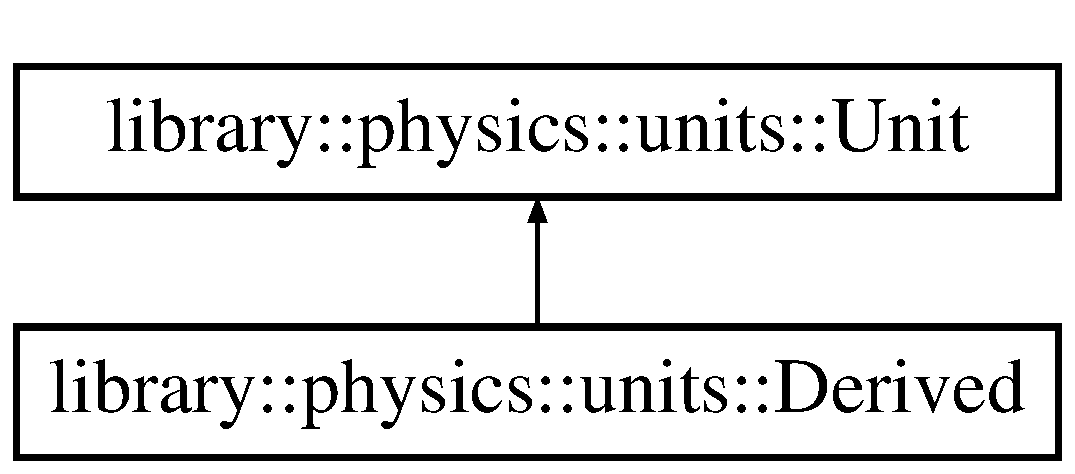
\includegraphics[height=2.000000cm]{classlibrary_1_1physics_1_1units_1_1_derived}
\end{center}
\end{figure}
\subsection*{Classes}
\begin{DoxyCompactItemize}
\item 
class \hyperlink{classlibrary_1_1physics_1_1units_1_1_derived_1_1_order}{Order}
\begin{DoxyCompactList}\small\item\em SI unit order. \end{DoxyCompactList}\item 
class \hyperlink{classlibrary_1_1physics_1_1units_1_1_derived_1_1_unit}{Unit}
\begin{DoxyCompactList}\small\item\em \hyperlink{classlibrary_1_1physics_1_1units_1_1_derived_1_1_unit}{Unit}. \end{DoxyCompactList}\end{DoxyCompactItemize}
\subsection*{Public Member Functions}
\begin{DoxyCompactItemize}
\item 
\hyperlink{classlibrary_1_1physics_1_1units_1_1_derived_a526996552af20a987c045ced9bd87fc7}{Derived} (const Real \&a\+Value, const \hyperlink{classlibrary_1_1physics_1_1units_1_1_derived_1_1_unit}{Derived\+::\+Unit} \&a\+Unit)
\begin{DoxyCompactList}\small\item\em Constructor. \end{DoxyCompactList}\item 
bool \hyperlink{classlibrary_1_1physics_1_1units_1_1_derived_a2cee9ae2cea2395bf21e377ee62eac67}{operator==} (const \hyperlink{classlibrary_1_1physics_1_1units_1_1_derived}{Derived} \&a\+Derived\+Unit) const
\item 
bool \hyperlink{classlibrary_1_1physics_1_1units_1_1_derived_a94357c9467421aabdc0a78423e2eef69}{operator!=} (const \hyperlink{classlibrary_1_1physics_1_1units_1_1_derived}{Derived} \&a\+Derived\+Unit) const
\item 
virtual bool \hyperlink{classlibrary_1_1physics_1_1units_1_1_derived_a26c20c57fc3a7c2fb2ff215d6d4687a2}{is\+Defined} () const override
\item 
\hyperlink{classlibrary_1_1physics_1_1units_1_1_derived_1_1_unit}{Derived\+::\+Unit} \hyperlink{classlibrary_1_1physics_1_1units_1_1_derived_a020b4ab6cb1d2ed73b01cde2bf1aab0e}{get\+Unit} () const
\item 
Real \hyperlink{classlibrary_1_1physics_1_1units_1_1_derived_a6ea039897b7a5905b096db05e392c484}{in} (const \hyperlink{classlibrary_1_1physics_1_1units_1_1_derived_1_1_unit}{Derived\+::\+Unit} \&a\+Unit) const
\item 
virtual String \hyperlink{classlibrary_1_1physics_1_1units_1_1_derived_a3626d6c77e6753f44232067856fde9d1}{to\+String} (const Integer \&a\+Precision=Integer\+::\+Undefined()) const override
\end{DoxyCompactItemize}
\subsection*{Static Public Member Functions}
\begin{DoxyCompactItemize}
\item 
static \hyperlink{classlibrary_1_1physics_1_1units_1_1_derived}{Derived} \hyperlink{classlibrary_1_1physics_1_1units_1_1_derived_a6b6d1cdd9a736856d213504e2b04fe4c}{Undefined} ()
\item 
static \hyperlink{classlibrary_1_1physics_1_1units_1_1_derived}{Derived} \hyperlink{classlibrary_1_1physics_1_1units_1_1_derived_a45b4ceae1f94e6877d15e67bf97572ee}{Parse} (const String \&a\+String)
\item 
static String \hyperlink{classlibrary_1_1physics_1_1units_1_1_derived_aca817ec7752af10f66c14f94467cf546}{String\+From\+Unit} (const \hyperlink{classlibrary_1_1physics_1_1units_1_1_derived_1_1_unit}{Derived\+::\+Unit} \&a\+Unit)
\item 
static String \hyperlink{classlibrary_1_1physics_1_1units_1_1_derived_a4c11c10b784fbb12cdae01125091a386}{Symbol\+From\+Unit} (const \hyperlink{classlibrary_1_1physics_1_1units_1_1_derived_1_1_unit}{Derived\+::\+Unit} \&a\+Unit)
\end{DoxyCompactItemize}
\subsection*{Friends}
\begin{DoxyCompactItemize}
\item 
std\+::ostream \& \hyperlink{classlibrary_1_1physics_1_1units_1_1_derived_a033deb6664987f4b2f86f5abeb18da81}{operator$<$$<$} (std\+::ostream \&an\+Output\+Stream, const \hyperlink{classlibrary_1_1physics_1_1units_1_1_derived}{Derived} \&a\+Derived\+Unit)
\end{DoxyCompactItemize}
\subsection*{Additional Inherited Members}


\subsection{Detailed Description}
\hyperlink{classlibrary_1_1physics_1_1units_1_1_derived}{Derived} unit. 

https\+://en.wikipedia.\+org/wiki/\+S\+I\+\_\+derived\+\_\+unit 

\subsection{Constructor \& Destructor Documentation}
\mbox{\Hypertarget{classlibrary_1_1physics_1_1units_1_1_derived_a526996552af20a987c045ced9bd87fc7}\label{classlibrary_1_1physics_1_1units_1_1_derived_a526996552af20a987c045ced9bd87fc7}} 
\index{library\+::physics\+::units\+::\+Derived@{library\+::physics\+::units\+::\+Derived}!Derived@{Derived}}
\index{Derived@{Derived}!library\+::physics\+::units\+::\+Derived@{library\+::physics\+::units\+::\+Derived}}
\subsubsection{\texorpdfstring{Derived()}{Derived()}}
{\footnotesize\ttfamily library\+::physics\+::units\+::\+Derived\+::\+Derived (\begin{DoxyParamCaption}\item[{const Real \&}]{a\+Value,  }\item[{const \hyperlink{classlibrary_1_1physics_1_1units_1_1_derived_1_1_unit}{Derived\+::\+Unit} \&}]{a\+Unit }\end{DoxyParamCaption})}



Constructor. 


\begin{DoxyCode}
\end{DoxyCode}



\begin{DoxyParams}[1]{Parameters}
\mbox{\tt in}  & {\em } & \\
\hline
\end{DoxyParams}


\subsection{Member Function Documentation}
\mbox{\Hypertarget{classlibrary_1_1physics_1_1units_1_1_derived_a020b4ab6cb1d2ed73b01cde2bf1aab0e}\label{classlibrary_1_1physics_1_1units_1_1_derived_a020b4ab6cb1d2ed73b01cde2bf1aab0e}} 
\index{library\+::physics\+::units\+::\+Derived@{library\+::physics\+::units\+::\+Derived}!get\+Unit@{get\+Unit}}
\index{get\+Unit@{get\+Unit}!library\+::physics\+::units\+::\+Derived@{library\+::physics\+::units\+::\+Derived}}
\subsubsection{\texorpdfstring{get\+Unit()}{getUnit()}}
{\footnotesize\ttfamily \hyperlink{classlibrary_1_1physics_1_1units_1_1_derived_1_1_unit}{Derived\+::\+Unit} library\+::physics\+::units\+::\+Derived\+::get\+Unit (\begin{DoxyParamCaption}{ }\end{DoxyParamCaption}) const}

\mbox{\Hypertarget{classlibrary_1_1physics_1_1units_1_1_derived_a6ea039897b7a5905b096db05e392c484}\label{classlibrary_1_1physics_1_1units_1_1_derived_a6ea039897b7a5905b096db05e392c484}} 
\index{library\+::physics\+::units\+::\+Derived@{library\+::physics\+::units\+::\+Derived}!in@{in}}
\index{in@{in}!library\+::physics\+::units\+::\+Derived@{library\+::physics\+::units\+::\+Derived}}
\subsubsection{\texorpdfstring{in()}{in()}}
{\footnotesize\ttfamily Real library\+::physics\+::units\+::\+Derived\+::in (\begin{DoxyParamCaption}\item[{const \hyperlink{classlibrary_1_1physics_1_1units_1_1_derived_1_1_unit}{Derived\+::\+Unit} \&}]{a\+Unit }\end{DoxyParamCaption}) const}

\mbox{\Hypertarget{classlibrary_1_1physics_1_1units_1_1_derived_a26c20c57fc3a7c2fb2ff215d6d4687a2}\label{classlibrary_1_1physics_1_1units_1_1_derived_a26c20c57fc3a7c2fb2ff215d6d4687a2}} 
\index{library\+::physics\+::units\+::\+Derived@{library\+::physics\+::units\+::\+Derived}!is\+Defined@{is\+Defined}}
\index{is\+Defined@{is\+Defined}!library\+::physics\+::units\+::\+Derived@{library\+::physics\+::units\+::\+Derived}}
\subsubsection{\texorpdfstring{is\+Defined()}{isDefined()}}
{\footnotesize\ttfamily bool library\+::physics\+::units\+::\+Derived\+::is\+Defined (\begin{DoxyParamCaption}{ }\end{DoxyParamCaption}) const\hspace{0.3cm}{\ttfamily [override]}, {\ttfamily [virtual]}}



Reimplemented from \hyperlink{classlibrary_1_1physics_1_1units_1_1_unit_a5ce011c1ffa0fce4cf1f5d42ff06ee78}{library\+::physics\+::units\+::\+Unit}.

\mbox{\Hypertarget{classlibrary_1_1physics_1_1units_1_1_derived_a94357c9467421aabdc0a78423e2eef69}\label{classlibrary_1_1physics_1_1units_1_1_derived_a94357c9467421aabdc0a78423e2eef69}} 
\index{library\+::physics\+::units\+::\+Derived@{library\+::physics\+::units\+::\+Derived}!operator"!=@{operator"!=}}
\index{operator"!=@{operator"!=}!library\+::physics\+::units\+::\+Derived@{library\+::physics\+::units\+::\+Derived}}
\subsubsection{\texorpdfstring{operator"!=()}{operator!=()}}
{\footnotesize\ttfamily bool library\+::physics\+::units\+::\+Derived\+::operator!= (\begin{DoxyParamCaption}\item[{const \hyperlink{classlibrary_1_1physics_1_1units_1_1_derived}{Derived} \&}]{a\+Derived\+Unit }\end{DoxyParamCaption}) const}

\mbox{\Hypertarget{classlibrary_1_1physics_1_1units_1_1_derived_a2cee9ae2cea2395bf21e377ee62eac67}\label{classlibrary_1_1physics_1_1units_1_1_derived_a2cee9ae2cea2395bf21e377ee62eac67}} 
\index{library\+::physics\+::units\+::\+Derived@{library\+::physics\+::units\+::\+Derived}!operator==@{operator==}}
\index{operator==@{operator==}!library\+::physics\+::units\+::\+Derived@{library\+::physics\+::units\+::\+Derived}}
\subsubsection{\texorpdfstring{operator==()}{operator==()}}
{\footnotesize\ttfamily bool library\+::physics\+::units\+::\+Derived\+::operator== (\begin{DoxyParamCaption}\item[{const \hyperlink{classlibrary_1_1physics_1_1units_1_1_derived}{Derived} \&}]{a\+Derived\+Unit }\end{DoxyParamCaption}) const}

\mbox{\Hypertarget{classlibrary_1_1physics_1_1units_1_1_derived_a45b4ceae1f94e6877d15e67bf97572ee}\label{classlibrary_1_1physics_1_1units_1_1_derived_a45b4ceae1f94e6877d15e67bf97572ee}} 
\index{library\+::physics\+::units\+::\+Derived@{library\+::physics\+::units\+::\+Derived}!Parse@{Parse}}
\index{Parse@{Parse}!library\+::physics\+::units\+::\+Derived@{library\+::physics\+::units\+::\+Derived}}
\subsubsection{\texorpdfstring{Parse()}{Parse()}}
{\footnotesize\ttfamily static \hyperlink{classlibrary_1_1physics_1_1units_1_1_derived}{Derived} library\+::physics\+::units\+::\+Derived\+::\+Parse (\begin{DoxyParamCaption}\item[{const String \&}]{a\+String }\end{DoxyParamCaption})\hspace{0.3cm}{\ttfamily [static]}}

\mbox{\Hypertarget{classlibrary_1_1physics_1_1units_1_1_derived_aca817ec7752af10f66c14f94467cf546}\label{classlibrary_1_1physics_1_1units_1_1_derived_aca817ec7752af10f66c14f94467cf546}} 
\index{library\+::physics\+::units\+::\+Derived@{library\+::physics\+::units\+::\+Derived}!String\+From\+Unit@{String\+From\+Unit}}
\index{String\+From\+Unit@{String\+From\+Unit}!library\+::physics\+::units\+::\+Derived@{library\+::physics\+::units\+::\+Derived}}
\subsubsection{\texorpdfstring{String\+From\+Unit()}{StringFromUnit()}}
{\footnotesize\ttfamily String library\+::physics\+::units\+::\+Derived\+::\+String\+From\+Unit (\begin{DoxyParamCaption}\item[{const \hyperlink{classlibrary_1_1physics_1_1units_1_1_derived_1_1_unit}{Derived\+::\+Unit} \&}]{a\+Unit }\end{DoxyParamCaption})\hspace{0.3cm}{\ttfamily [static]}}

\mbox{\Hypertarget{classlibrary_1_1physics_1_1units_1_1_derived_a4c11c10b784fbb12cdae01125091a386}\label{classlibrary_1_1physics_1_1units_1_1_derived_a4c11c10b784fbb12cdae01125091a386}} 
\index{library\+::physics\+::units\+::\+Derived@{library\+::physics\+::units\+::\+Derived}!Symbol\+From\+Unit@{Symbol\+From\+Unit}}
\index{Symbol\+From\+Unit@{Symbol\+From\+Unit}!library\+::physics\+::units\+::\+Derived@{library\+::physics\+::units\+::\+Derived}}
\subsubsection{\texorpdfstring{Symbol\+From\+Unit()}{SymbolFromUnit()}}
{\footnotesize\ttfamily String library\+::physics\+::units\+::\+Derived\+::\+Symbol\+From\+Unit (\begin{DoxyParamCaption}\item[{const \hyperlink{classlibrary_1_1physics_1_1units_1_1_derived_1_1_unit}{Derived\+::\+Unit} \&}]{a\+Unit }\end{DoxyParamCaption})\hspace{0.3cm}{\ttfamily [static]}}

\mbox{\Hypertarget{classlibrary_1_1physics_1_1units_1_1_derived_a3626d6c77e6753f44232067856fde9d1}\label{classlibrary_1_1physics_1_1units_1_1_derived_a3626d6c77e6753f44232067856fde9d1}} 
\index{library\+::physics\+::units\+::\+Derived@{library\+::physics\+::units\+::\+Derived}!to\+String@{to\+String}}
\index{to\+String@{to\+String}!library\+::physics\+::units\+::\+Derived@{library\+::physics\+::units\+::\+Derived}}
\subsubsection{\texorpdfstring{to\+String()}{toString()}}
{\footnotesize\ttfamily String library\+::physics\+::units\+::\+Derived\+::to\+String (\begin{DoxyParamCaption}\item[{const Integer \&}]{a\+Precision = {\ttfamily Integer\+:\+:Undefined()} }\end{DoxyParamCaption}) const\hspace{0.3cm}{\ttfamily [override]}, {\ttfamily [virtual]}}



Implements \hyperlink{classlibrary_1_1physics_1_1units_1_1_unit_aac05cb6ed1ea7c18c233a3381c81caf8}{library\+::physics\+::units\+::\+Unit}.

\mbox{\Hypertarget{classlibrary_1_1physics_1_1units_1_1_derived_a6b6d1cdd9a736856d213504e2b04fe4c}\label{classlibrary_1_1physics_1_1units_1_1_derived_a6b6d1cdd9a736856d213504e2b04fe4c}} 
\index{library\+::physics\+::units\+::\+Derived@{library\+::physics\+::units\+::\+Derived}!Undefined@{Undefined}}
\index{Undefined@{Undefined}!library\+::physics\+::units\+::\+Derived@{library\+::physics\+::units\+::\+Derived}}
\subsubsection{\texorpdfstring{Undefined()}{Undefined()}}
{\footnotesize\ttfamily \hyperlink{classlibrary_1_1physics_1_1units_1_1_derived}{Derived} library\+::physics\+::units\+::\+Derived\+::\+Undefined (\begin{DoxyParamCaption}{ }\end{DoxyParamCaption})\hspace{0.3cm}{\ttfamily [static]}}



\subsection{Friends And Related Function Documentation}
\mbox{\Hypertarget{classlibrary_1_1physics_1_1units_1_1_derived_a033deb6664987f4b2f86f5abeb18da81}\label{classlibrary_1_1physics_1_1units_1_1_derived_a033deb6664987f4b2f86f5abeb18da81}} 
\index{library\+::physics\+::units\+::\+Derived@{library\+::physics\+::units\+::\+Derived}!operator$<$$<$@{operator$<$$<$}}
\index{operator$<$$<$@{operator$<$$<$}!library\+::physics\+::units\+::\+Derived@{library\+::physics\+::units\+::\+Derived}}
\subsubsection{\texorpdfstring{operator$<$$<$}{operator<<}}
{\footnotesize\ttfamily std\+::ostream\& operator$<$$<$ (\begin{DoxyParamCaption}\item[{std\+::ostream \&}]{an\+Output\+Stream,  }\item[{const \hyperlink{classlibrary_1_1physics_1_1units_1_1_derived}{Derived} \&}]{a\+Derived\+Unit }\end{DoxyParamCaption})\hspace{0.3cm}{\ttfamily [friend]}}



The documentation for this class was generated from the following files\+:\begin{DoxyCompactItemize}
\item 
include/\+Library/\+Physics/\+Units/\hyperlink{_derived_8hpp}{Derived.\+hpp}\item 
src/\+Library/\+Physics/\+Units/\hyperlink{_derived_8cpp}{Derived.\+cpp}\end{DoxyCompactItemize}

\hypertarget{classlibrary_1_1physics_1_1time_1_1_duration}{}\section{library\+:\+:physics\+:\+:time\+:\+:Duration Class Reference}
\label{classlibrary_1_1physics_1_1time_1_1_duration}\index{library\+::physics\+::time\+::\+Duration@{library\+::physics\+::time\+::\+Duration}}


Amount of time.  




{\ttfamily \#include $<$Duration.\+hpp$>$}

\subsection*{Public Types}
\begin{DoxyCompactItemize}
\item 
enum \hyperlink{classlibrary_1_1physics_1_1time_1_1_duration_ace85659cafe97df992c0e4273bdc88d1}{Format} \{ \hyperlink{classlibrary_1_1physics_1_1time_1_1_duration_ace85659cafe97df992c0e4273bdc88d1aec0fc0100c4fc1ce4eea230c3dc10360}{Format\+::\+Undefined}, 
\hyperlink{classlibrary_1_1physics_1_1time_1_1_duration_ace85659cafe97df992c0e4273bdc88d1aeb6d8ae6f20283755b339c0dc273988b}{Format\+::\+Standard}, 
\hyperlink{classlibrary_1_1physics_1_1time_1_1_duration_ace85659cafe97df992c0e4273bdc88d1a35b6786739efcdc5a74ab1dca29d3b6b}{Format\+::\+I\+S\+O8601}
 \}\begin{DoxyCompactList}\small\item\em \hyperlink{classlibrary_1_1physics_1_1time_1_1_duration}{Duration} format. \end{DoxyCompactList}
\end{DoxyCompactItemize}
\subsection*{Public Member Functions}
\begin{DoxyCompactItemize}
\item 
\hyperlink{classlibrary_1_1physics_1_1time_1_1_duration_a0a70efcf487a841da572afcf00001f64}{Duration} (Int64 a\+Nanosecond\+Count)
\begin{DoxyCompactList}\small\item\em Constructor. \end{DoxyCompactList}\item 
bool \hyperlink{classlibrary_1_1physics_1_1time_1_1_duration_ac368d2fe8d2a04248dac2b53bdfbfb21}{operator==} (const \hyperlink{classlibrary_1_1physics_1_1time_1_1_duration}{Duration} \&a\+Duration) const
\begin{DoxyCompactList}\small\item\em Equal to operator. \end{DoxyCompactList}\item 
bool \hyperlink{classlibrary_1_1physics_1_1time_1_1_duration_a620feff807a95ea439fdfdd5cf5490b2}{operator!=} (const \hyperlink{classlibrary_1_1physics_1_1time_1_1_duration}{Duration} \&a\+Duration) const
\begin{DoxyCompactList}\small\item\em Not equal to operator. \end{DoxyCompactList}\item 
bool \hyperlink{classlibrary_1_1physics_1_1time_1_1_duration_a90fbdc66d103d7ce07122224db6fc1d9}{operator$<$} (const \hyperlink{classlibrary_1_1physics_1_1time_1_1_duration}{Duration} \&a\+Duration) const
\begin{DoxyCompactList}\small\item\em Less than operator. \end{DoxyCompactList}\item 
bool \hyperlink{classlibrary_1_1physics_1_1time_1_1_duration_a95d806324b7235b0dec175bde4996e7c}{operator$<$=} (const \hyperlink{classlibrary_1_1physics_1_1time_1_1_duration}{Duration} \&a\+Duration) const
\begin{DoxyCompactList}\small\item\em Less than or equal to operator. \end{DoxyCompactList}\item 
bool \hyperlink{classlibrary_1_1physics_1_1time_1_1_duration_ac7fa93e402efc7c23f1acb8df9b54c79}{operator$>$} (const \hyperlink{classlibrary_1_1physics_1_1time_1_1_duration}{Duration} \&a\+Duration) const
\begin{DoxyCompactList}\small\item\em Greater than operator. \end{DoxyCompactList}\item 
bool \hyperlink{classlibrary_1_1physics_1_1time_1_1_duration_a4338d704712640124d44a6e7a52909ea}{operator$>$=} (const \hyperlink{classlibrary_1_1physics_1_1time_1_1_duration}{Duration} \&a\+Duration) const
\begin{DoxyCompactList}\small\item\em Greater than operator. \end{DoxyCompactList}\item 
\hyperlink{classlibrary_1_1physics_1_1time_1_1_duration}{Duration} \hyperlink{classlibrary_1_1physics_1_1time_1_1_duration_ae130ab9904fc08b9cf19b32510913350}{operator+} (const \hyperlink{classlibrary_1_1physics_1_1time_1_1_duration}{Duration} \&a\+Duration) const
\begin{DoxyCompactList}\small\item\em Addition operator. \end{DoxyCompactList}\item 
\hyperlink{classlibrary_1_1physics_1_1time_1_1_duration}{Duration} \hyperlink{classlibrary_1_1physics_1_1time_1_1_duration_a9d45bbc3db56c0163bb5d33c41888879}{operator-\/} (const \hyperlink{classlibrary_1_1physics_1_1time_1_1_duration}{Duration} \&a\+Duration) const
\begin{DoxyCompactList}\small\item\em Subtraction operator. \end{DoxyCompactList}\item 
\hyperlink{classlibrary_1_1physics_1_1time_1_1_duration}{Duration} \hyperlink{classlibrary_1_1physics_1_1time_1_1_duration_a6aea6dbe11b3199e63ee29a851c3fc16}{operator$\ast$} (const Real \&a\+Multiplier) const
\begin{DoxyCompactList}\small\item\em Multiplication operator. \end{DoxyCompactList}\item 
\hyperlink{classlibrary_1_1physics_1_1time_1_1_duration}{Duration} \hyperlink{classlibrary_1_1physics_1_1time_1_1_duration_aa1488a4b12024ff181631951758676be}{operator/} (const Real \&a\+Divider) const
\begin{DoxyCompactList}\small\item\em Division operator. \end{DoxyCompactList}\item 
\hyperlink{classlibrary_1_1physics_1_1time_1_1_duration}{Duration} \hyperlink{classlibrary_1_1physics_1_1time_1_1_duration_a315c20670e53373e2d9f47ff07c6c09c}{operator+} () const
\begin{DoxyCompactList}\small\item\em Unary plus operator. \end{DoxyCompactList}\item 
\hyperlink{classlibrary_1_1physics_1_1time_1_1_duration}{Duration} \hyperlink{classlibrary_1_1physics_1_1time_1_1_duration_a9f2fa54832b4ef58c48167c80285bad2}{operator-\/} () const
\begin{DoxyCompactList}\small\item\em Unary minus operator. \end{DoxyCompactList}\item 
\hyperlink{classlibrary_1_1physics_1_1time_1_1_duration}{Duration} \& \hyperlink{classlibrary_1_1physics_1_1time_1_1_duration_a2d2848688c326591ea1a406e5a0275d0}{operator+=} (const \hyperlink{classlibrary_1_1physics_1_1time_1_1_duration}{Duration} \&a\+Duration)
\begin{DoxyCompactList}\small\item\em Addition assignement operator. \end{DoxyCompactList}\item 
\hyperlink{classlibrary_1_1physics_1_1time_1_1_duration}{Duration} \& \hyperlink{classlibrary_1_1physics_1_1time_1_1_duration_a49e7a4be10cf8cade127314a80b4180e}{operator-\/=} (const \hyperlink{classlibrary_1_1physics_1_1time_1_1_duration}{Duration} \&a\+Duration)
\begin{DoxyCompactList}\small\item\em Subtraction assignement operator. \end{DoxyCompactList}\item 
\hyperlink{classlibrary_1_1physics_1_1time_1_1_duration}{Duration} \& \hyperlink{classlibrary_1_1physics_1_1time_1_1_duration_a510b18495d52c34ebd34e3bb9bf723e6}{operator$\ast$=} (const Real \&a\+Multiplier)
\begin{DoxyCompactList}\small\item\em Multiplication assignement operator. \end{DoxyCompactList}\item 
\hyperlink{classlibrary_1_1physics_1_1time_1_1_duration}{Duration} \& \hyperlink{classlibrary_1_1physics_1_1time_1_1_duration_a0f57d9d0934d6851e3956744f2e85b48}{operator/=} (const Real \&a\+Divider)
\begin{DoxyCompactList}\small\item\em Division assignement operator. \end{DoxyCompactList}\item 
bool \hyperlink{classlibrary_1_1physics_1_1time_1_1_duration_af6ee4c1644a1cafc96d670e576dc6749}{is\+Defined} () const
\begin{DoxyCompactList}\small\item\em Check if duration is defined. \end{DoxyCompactList}\item 
bool \hyperlink{classlibrary_1_1physics_1_1time_1_1_duration_a7f14980ea22f7e9cad122f7a37ba50be}{is\+Zero} () const
\begin{DoxyCompactList}\small\item\em Check if duration is zero. \end{DoxyCompactList}\item 
bool \hyperlink{classlibrary_1_1physics_1_1time_1_1_duration_a443d719fb2acf922cc80a8f2be441fa1}{is\+Positive} () const
\begin{DoxyCompactList}\small\item\em Check if duration is positive. \end{DoxyCompactList}\item 
bool \hyperlink{classlibrary_1_1physics_1_1time_1_1_duration_a2d4f7691e997232d4d9b88e7d4ab49d7}{is\+Strictly\+Positive} () const
\begin{DoxyCompactList}\small\item\em Check if duration is strictly positive. \end{DoxyCompactList}\item 
bool \hyperlink{classlibrary_1_1physics_1_1time_1_1_duration_a7df03d520e9372f58c37309e8ac8e08d}{is\+Near} (const \hyperlink{classlibrary_1_1physics_1_1time_1_1_duration}{Duration} \&a\+Duration, const \hyperlink{classlibrary_1_1physics_1_1time_1_1_duration}{Duration} \&a\+Tolerance) const
\begin{DoxyCompactList}\small\item\em Check if duration is near another duration. \end{DoxyCompactList}\item 
Integer \hyperlink{classlibrary_1_1physics_1_1time_1_1_duration_a5dad1e24c78cd7ef13a4220eb4e73dd0}{get\+Nanoseconds} () const
\begin{DoxyCompactList}\small\item\em Get the number of nanoseconds in duration. \end{DoxyCompactList}\item 
Integer \hyperlink{classlibrary_1_1physics_1_1time_1_1_duration_a65db73a28d87e3f06d307cbd688739a3}{get\+Microseconds} () const
\begin{DoxyCompactList}\small\item\em Get the number of microseconds in duration. \end{DoxyCompactList}\item 
Integer \hyperlink{classlibrary_1_1physics_1_1time_1_1_duration_aac5063bb791db96348e23784106a4eba}{get\+Milliseconds} () const
\begin{DoxyCompactList}\small\item\em Get the number of milliseconds in duration. \end{DoxyCompactList}\item 
Integer \hyperlink{classlibrary_1_1physics_1_1time_1_1_duration_a98388bab81d1d5550532fdedaa08635c}{get\+Seconds} () const
\begin{DoxyCompactList}\small\item\em Get the number of seconds in duration. \end{DoxyCompactList}\item 
Integer \hyperlink{classlibrary_1_1physics_1_1time_1_1_duration_a2c8a5767f1a0add4999c649001cdb838}{get\+Minutes} () const
\begin{DoxyCompactList}\small\item\em Get the number of minutes in duration. \end{DoxyCompactList}\item 
Integer \hyperlink{classlibrary_1_1physics_1_1time_1_1_duration_a05ef46de76556cd571fd8a218dc3b24f}{get\+Hours} () const
\begin{DoxyCompactList}\small\item\em Get the number of hours in duration. \end{DoxyCompactList}\item 
Integer \hyperlink{classlibrary_1_1physics_1_1time_1_1_duration_a06ffb87b3c946a64a69000784488ab5c}{get\+Days} () const
\begin{DoxyCompactList}\small\item\em Get the number of days in duration. \end{DoxyCompactList}\item 
Integer \hyperlink{classlibrary_1_1physics_1_1time_1_1_duration_a11cf17341b43110b443ffd150571f43c}{get\+Weeks} () const
\begin{DoxyCompactList}\small\item\em Get the number of weeks in duration. \end{DoxyCompactList}\item 
Real \hyperlink{classlibrary_1_1physics_1_1time_1_1_duration_a45aa358d61481356dd591290d6ab3691}{in\+Nanoseconds} () const
\begin{DoxyCompactList}\small\item\em Get nanosecond count. \end{DoxyCompactList}\item 
Real \hyperlink{classlibrary_1_1physics_1_1time_1_1_duration_a69c9501a4432aac49cecd9d47da7c4f6}{in\+Microseconds} () const
\begin{DoxyCompactList}\small\item\em Get microsecond count. \end{DoxyCompactList}\item 
Real \hyperlink{classlibrary_1_1physics_1_1time_1_1_duration_ac7c1fce0e8488954fe9e2abe1767548b}{in\+Milliseconds} () const
\begin{DoxyCompactList}\small\item\em Get millisecond count. \end{DoxyCompactList}\item 
Real \hyperlink{classlibrary_1_1physics_1_1time_1_1_duration_a9272debd96e7f86df9b0852c6663a0bb}{in\+Seconds} () const
\begin{DoxyCompactList}\small\item\em Get second count. \end{DoxyCompactList}\item 
Real \hyperlink{classlibrary_1_1physics_1_1time_1_1_duration_aef580516014096d1e5ae5bb6ae8e6f29}{in\+Minutes} () const
\begin{DoxyCompactList}\small\item\em Get minute count. \end{DoxyCompactList}\item 
Real \hyperlink{classlibrary_1_1physics_1_1time_1_1_duration_a1f5e207d7c6f7b62d3cfee13e75dfa48}{in\+Hours} () const
\begin{DoxyCompactList}\small\item\em Get hour count. \end{DoxyCompactList}\item 
Real \hyperlink{classlibrary_1_1physics_1_1time_1_1_duration_a73ebd929416f360ff5c4c840fbcae67b}{in\+Days} () const
\begin{DoxyCompactList}\small\item\em Get day count. \end{DoxyCompactList}\item 
Real \hyperlink{classlibrary_1_1physics_1_1time_1_1_duration_ae49243cf87ccf07693b65e7170642b65}{in\+Weeks} () const
\begin{DoxyCompactList}\small\item\em Get week count. \end{DoxyCompactList}\item 
Real \hyperlink{classlibrary_1_1physics_1_1time_1_1_duration_ace9b1e589d3dc6e76002d389e2a480df}{in} (const \hyperlink{classlibrary_1_1physics_1_1units_1_1_time_ab876a6a05c9a2f28905f2753bfd64109}{units\+::\+Time\+::\+Unit} \&a\+Time\+Unit) const
\begin{DoxyCompactList}\small\item\em Get count in given time unit. \end{DoxyCompactList}\item 
\hyperlink{classlibrary_1_1physics_1_1time_1_1_duration}{Duration} \hyperlink{classlibrary_1_1physics_1_1time_1_1_duration_afbe401469b6b6356439d6f7c5b21e67e}{get\+Absolute} () const
\begin{DoxyCompactList}\small\item\em Get absolute duration. \end{DoxyCompactList}\item 
String \hyperlink{classlibrary_1_1physics_1_1time_1_1_duration_a06f24e6cc8cb867abbae969c5f199513}{to\+String} (const \hyperlink{classlibrary_1_1physics_1_1time_1_1_duration_ace85659cafe97df992c0e4273bdc88d1}{Duration\+::\+Format} \&a\+Format=\hyperlink{classlibrary_1_1physics_1_1time_1_1_duration_ace85659cafe97df992c0e4273bdc88d1aeb6d8ae6f20283755b339c0dc273988b}{Duration\+::\+Format\+::\+Standard}) const
\begin{DoxyCompactList}\small\item\em Get string representation of duration. \end{DoxyCompactList}\end{DoxyCompactItemize}
\subsection*{Static Public Member Functions}
\begin{DoxyCompactItemize}
\item 
static \hyperlink{classlibrary_1_1physics_1_1time_1_1_duration}{Duration} \hyperlink{classlibrary_1_1physics_1_1time_1_1_duration_a67012781d9b7491e26bdc3da9f513130}{Undefined} ()
\begin{DoxyCompactList}\small\item\em Constructs an undefined duration. \end{DoxyCompactList}\item 
static \hyperlink{classlibrary_1_1physics_1_1time_1_1_duration}{Duration} \hyperlink{classlibrary_1_1physics_1_1time_1_1_duration_aa68c3998cd4cf9068fb239dd66102c2c}{Zero} ()
\begin{DoxyCompactList}\small\item\em Constructs a zero duration. \end{DoxyCompactList}\item 
static \hyperlink{classlibrary_1_1physics_1_1time_1_1_duration}{Duration} \hyperlink{classlibrary_1_1physics_1_1time_1_1_duration_a6a629b2275337fbadac912cc9364a9f1}{Nanoseconds} (const Real \&a\+Nanosecond\+Count)
\begin{DoxyCompactList}\small\item\em Constructs a duration from a nanosecond count. \end{DoxyCompactList}\item 
static \hyperlink{classlibrary_1_1physics_1_1time_1_1_duration}{Duration} \hyperlink{classlibrary_1_1physics_1_1time_1_1_duration_a9082d43579a99fd667b0080de8adf8ed}{Microseconds} (const Real \&a\+Microsecond\+Count)
\begin{DoxyCompactList}\small\item\em Constructs a duration from a microsecond count. \end{DoxyCompactList}\item 
static \hyperlink{classlibrary_1_1physics_1_1time_1_1_duration}{Duration} \hyperlink{classlibrary_1_1physics_1_1time_1_1_duration_ab6eab798898a96019a8c944cd565e161}{Milliseconds} (const Real \&a\+Millisecond\+Count)
\begin{DoxyCompactList}\small\item\em Constructs a duration from a millisecond count. \end{DoxyCompactList}\item 
static \hyperlink{classlibrary_1_1physics_1_1time_1_1_duration}{Duration} \hyperlink{classlibrary_1_1physics_1_1time_1_1_duration_ae10891c94a1b2278c444cb44b37132f1}{Seconds} (const Real \&a\+Second\+Count)
\begin{DoxyCompactList}\small\item\em Constructs a duration from a second count. \end{DoxyCompactList}\item 
static \hyperlink{classlibrary_1_1physics_1_1time_1_1_duration}{Duration} \hyperlink{classlibrary_1_1physics_1_1time_1_1_duration_ad7171befa3075e796bfb02a7542dacdd}{Minutes} (const Real \&a\+Minute\+Count)
\begin{DoxyCompactList}\small\item\em Constructs a duration from a minute count. \end{DoxyCompactList}\item 
static \hyperlink{classlibrary_1_1physics_1_1time_1_1_duration}{Duration} \hyperlink{classlibrary_1_1physics_1_1time_1_1_duration_aadef86b1b803b8764380ef623f99ce95}{Hours} (const Real \&an\+Hour\+Count)
\begin{DoxyCompactList}\small\item\em Constructs a duration from a hour count. \end{DoxyCompactList}\item 
static \hyperlink{classlibrary_1_1physics_1_1time_1_1_duration}{Duration} \hyperlink{classlibrary_1_1physics_1_1time_1_1_duration_abf1323fa113b5203747ce9aec5c969fc}{Days} (const Real \&a\+Day\+Count)
\begin{DoxyCompactList}\small\item\em Constructs a duration from a day count. \end{DoxyCompactList}\item 
static \hyperlink{classlibrary_1_1physics_1_1time_1_1_duration}{Duration} \hyperlink{classlibrary_1_1physics_1_1time_1_1_duration_ae9d507f6cbb36902529b28d3721507c1}{Weeks} (const Real \&a\+Week\+Count)
\begin{DoxyCompactList}\small\item\em Constructs a duration from a week count. \end{DoxyCompactList}\item 
static \hyperlink{classlibrary_1_1physics_1_1time_1_1_duration}{Duration} \hyperlink{classlibrary_1_1physics_1_1time_1_1_duration_a7d2654965a46c6eff9d331ad8b0d9b1f}{Between} (const \hyperlink{classlibrary_1_1physics_1_1time_1_1_instant}{Instant} \&a\+First\+Instant, const \hyperlink{classlibrary_1_1physics_1_1time_1_1_instant}{Instant} \&a\+Second\+Instant)
\begin{DoxyCompactList}\small\item\em Constructs a duration between two instants. \end{DoxyCompactList}\item 
static \hyperlink{classlibrary_1_1physics_1_1time_1_1_duration}{Duration} \hyperlink{classlibrary_1_1physics_1_1time_1_1_duration_a52ba6dd2958d1e193b81d8f659bb6bf3}{Parse} (const String \&a\+String, const \hyperlink{classlibrary_1_1physics_1_1time_1_1_duration_ace85659cafe97df992c0e4273bdc88d1}{Duration\+::\+Format} \&a\+Format=\hyperlink{classlibrary_1_1physics_1_1time_1_1_duration_ace85659cafe97df992c0e4273bdc88d1aec0fc0100c4fc1ce4eea230c3dc10360}{Duration\+::\+Format\+::\+Undefined})
\begin{DoxyCompactList}\small\item\em Constructs a duration from a string representation. \end{DoxyCompactList}\end{DoxyCompactItemize}
\subsection*{Public Attributes}
\begin{DoxyCompactItemize}
\item 
friend \hyperlink{classlibrary_1_1physics_1_1time_1_1_duration_ac98d9996643dde64fe1ffe67c12cc945}{Instant}
\end{DoxyCompactItemize}
\subsection*{Friends}
\begin{DoxyCompactItemize}
\item 
\hyperlink{classlibrary_1_1physics_1_1time_1_1_duration}{Duration} \hyperlink{classlibrary_1_1physics_1_1time_1_1_duration_a30be5772f32cb400f8d8a8e2975abf6d}{operator$\ast$} (double a\+Multiplier, const \hyperlink{classlibrary_1_1physics_1_1time_1_1_duration}{Duration} \&a\+Duration)
\begin{DoxyCompactList}\small\item\em Multiplication operator. \end{DoxyCompactList}\item 
std\+::ostream \& \hyperlink{classlibrary_1_1physics_1_1time_1_1_duration_a82573aea35c8642b571f78c85ca70fbc}{operator$<$$<$} (std\+::ostream \&an\+Output\+Stream, const \hyperlink{classlibrary_1_1physics_1_1time_1_1_duration}{Duration} \&a\+Duration)
\begin{DoxyCompactList}\small\item\em Output stream operator. \end{DoxyCompactList}\end{DoxyCompactItemize}


\subsection{Detailed Description}
Amount of time. 

\subsection{Member Enumeration Documentation}
\mbox{\Hypertarget{classlibrary_1_1physics_1_1time_1_1_duration_ace85659cafe97df992c0e4273bdc88d1}\label{classlibrary_1_1physics_1_1time_1_1_duration_ace85659cafe97df992c0e4273bdc88d1}} 
\index{library\+::physics\+::time\+::\+Duration@{library\+::physics\+::time\+::\+Duration}!Format@{Format}}
\index{Format@{Format}!library\+::physics\+::time\+::\+Duration@{library\+::physics\+::time\+::\+Duration}}
\subsubsection{\texorpdfstring{Format}{Format}}
{\footnotesize\ttfamily enum \hyperlink{classlibrary_1_1physics_1_1time_1_1_duration_ace85659cafe97df992c0e4273bdc88d1}{library\+::physics\+::time\+::\+Duration\+::\+Format}\hspace{0.3cm}{\ttfamily [strong]}}



\hyperlink{classlibrary_1_1physics_1_1time_1_1_duration}{Duration} format. 

\begin{DoxyEnumFields}{Enumerator}
\raisebox{\heightof{T}}[0pt][0pt]{\index{Undefined@{Undefined}!library\+::physics\+::time\+::\+Duration@{library\+::physics\+::time\+::\+Duration}}\index{library\+::physics\+::time\+::\+Duration@{library\+::physics\+::time\+::\+Duration}!Undefined@{Undefined}}}\mbox{\Hypertarget{classlibrary_1_1physics_1_1time_1_1_duration_ace85659cafe97df992c0e4273bdc88d1aec0fc0100c4fc1ce4eea230c3dc10360}\label{classlibrary_1_1physics_1_1time_1_1_duration_ace85659cafe97df992c0e4273bdc88d1aec0fc0100c4fc1ce4eea230c3dc10360}} 
Undefined&Undefined format. \\
\hline

\raisebox{\heightof{T}}[0pt][0pt]{\index{Standard@{Standard}!library\+::physics\+::time\+::\+Duration@{library\+::physics\+::time\+::\+Duration}}\index{library\+::physics\+::time\+::\+Duration@{library\+::physics\+::time\+::\+Duration}!Standard@{Standard}}}\mbox{\Hypertarget{classlibrary_1_1physics_1_1time_1_1_duration_ace85659cafe97df992c0e4273bdc88d1aeb6d8ae6f20283755b339c0dc273988b}\label{classlibrary_1_1physics_1_1time_1_1_duration_ace85659cafe97df992c0e4273bdc88d1aeb6d8ae6f20283755b339c0dc273988b}} 
Standard&Standard format (d hh\+:mm\+:ss.\+mmm.\+uuu.\+nnn) \\
\hline

\raisebox{\heightof{T}}[0pt][0pt]{\index{I\+S\+O8601@{I\+S\+O8601}!library\+::physics\+::time\+::\+Duration@{library\+::physics\+::time\+::\+Duration}}\index{library\+::physics\+::time\+::\+Duration@{library\+::physics\+::time\+::\+Duration}!I\+S\+O8601@{I\+S\+O8601}}}\mbox{\Hypertarget{classlibrary_1_1physics_1_1time_1_1_duration_ace85659cafe97df992c0e4273bdc88d1a35b6786739efcdc5a74ab1dca29d3b6b}\label{classlibrary_1_1physics_1_1time_1_1_duration_ace85659cafe97df992c0e4273bdc88d1a35b6786739efcdc5a74ab1dca29d3b6b}} 
I\+S\+O8601&I\+SO 8601 format (Pn\+D\+Tn\+Hn\+MnS) \\
\hline

\end{DoxyEnumFields}


\subsection{Constructor \& Destructor Documentation}
\mbox{\Hypertarget{classlibrary_1_1physics_1_1time_1_1_duration_a0a70efcf487a841da572afcf00001f64}\label{classlibrary_1_1physics_1_1time_1_1_duration_a0a70efcf487a841da572afcf00001f64}} 
\index{library\+::physics\+::time\+::\+Duration@{library\+::physics\+::time\+::\+Duration}!Duration@{Duration}}
\index{Duration@{Duration}!library\+::physics\+::time\+::\+Duration@{library\+::physics\+::time\+::\+Duration}}
\subsubsection{\texorpdfstring{Duration()}{Duration()}}
{\footnotesize\ttfamily library\+::physics\+::time\+::\+Duration\+::\+Duration (\begin{DoxyParamCaption}\item[{Int64}]{a\+Nanosecond\+Count }\end{DoxyParamCaption})}



Constructor. 


\begin{DoxyCode}
\hyperlink{classlibrary_1_1physics_1_1time_1_1_duration_a0a70efcf487a841da572afcf00001f64}{Duration} duration(123) ; \textcolor{comment}{// 123 [ns]}
\end{DoxyCode}
 
\begin{DoxyParams}[1]{Parameters}
\mbox{\tt in}  & {\em a\+Nanosecond\+Count} & A nanosecond count \\
\hline
\end{DoxyParams}


\subsection{Member Function Documentation}
\mbox{\Hypertarget{classlibrary_1_1physics_1_1time_1_1_duration_a7d2654965a46c6eff9d331ad8b0d9b1f}\label{classlibrary_1_1physics_1_1time_1_1_duration_a7d2654965a46c6eff9d331ad8b0d9b1f}} 
\index{library\+::physics\+::time\+::\+Duration@{library\+::physics\+::time\+::\+Duration}!Between@{Between}}
\index{Between@{Between}!library\+::physics\+::time\+::\+Duration@{library\+::physics\+::time\+::\+Duration}}
\subsubsection{\texorpdfstring{Between()}{Between()}}
{\footnotesize\ttfamily \hyperlink{classlibrary_1_1physics_1_1time_1_1_duration}{Duration} library\+::physics\+::time\+::\+Duration\+::\+Between (\begin{DoxyParamCaption}\item[{const \hyperlink{classlibrary_1_1physics_1_1time_1_1_instant}{Instant} \&}]{a\+First\+Instant,  }\item[{const \hyperlink{classlibrary_1_1physics_1_1time_1_1_instant}{Instant} \&}]{a\+Second\+Instant }\end{DoxyParamCaption})\hspace{0.3cm}{\ttfamily [static]}}



Constructs a duration between two instants. 

\hyperlink{classlibrary_1_1physics_1_1time_1_1_duration}{Duration} is positive is first\+Instant $<$ second\+Instant.


\begin{DoxyCode}
\hyperlink{classlibrary_1_1physics_1_1time_1_1_duration_a0a70efcf487a841da572afcf00001f64}{Duration} duration = \hyperlink{classlibrary_1_1physics_1_1time_1_1_duration_a7d2654965a46c6eff9d331ad8b0d9b1f}{Duration::Between}(firstInstant, secondInstant) ;
\end{DoxyCode}



\begin{DoxyParams}[1]{Parameters}
\mbox{\tt in}  & {\em a\+First\+Instant} & A first instant \\
\hline
\mbox{\tt in}  & {\em a\+Second\+Instant} & A second instant \\
\hline
\end{DoxyParams}
\begin{DoxyReturn}{Returns}
\hyperlink{classlibrary_1_1physics_1_1time_1_1_duration}{Duration} 
\end{DoxyReturn}
\mbox{\Hypertarget{classlibrary_1_1physics_1_1time_1_1_duration_abf1323fa113b5203747ce9aec5c969fc}\label{classlibrary_1_1physics_1_1time_1_1_duration_abf1323fa113b5203747ce9aec5c969fc}} 
\index{library\+::physics\+::time\+::\+Duration@{library\+::physics\+::time\+::\+Duration}!Days@{Days}}
\index{Days@{Days}!library\+::physics\+::time\+::\+Duration@{library\+::physics\+::time\+::\+Duration}}
\subsubsection{\texorpdfstring{Days()}{Days()}}
{\footnotesize\ttfamily \hyperlink{classlibrary_1_1physics_1_1time_1_1_duration}{Duration} library\+::physics\+::time\+::\+Duration\+::\+Days (\begin{DoxyParamCaption}\item[{const Real \&}]{a\+Day\+Count }\end{DoxyParamCaption})\hspace{0.3cm}{\ttfamily [static]}}



Constructs a duration from a day count. 


\begin{DoxyCode}
\hyperlink{classlibrary_1_1physics_1_1time_1_1_duration_a0a70efcf487a841da572afcf00001f64}{Duration} duration = \hyperlink{classlibrary_1_1physics_1_1time_1_1_duration_abf1323fa113b5203747ce9aec5c969fc}{Duration::Days}(123) ;
\end{DoxyCode}



\begin{DoxyParams}[1]{Parameters}
\mbox{\tt in}  & {\em a\+Day\+Count} & A day count \\
\hline
\end{DoxyParams}
\begin{DoxyReturn}{Returns}
\hyperlink{classlibrary_1_1physics_1_1time_1_1_duration}{Duration} 
\end{DoxyReturn}
\mbox{\Hypertarget{classlibrary_1_1physics_1_1time_1_1_duration_afbe401469b6b6356439d6f7c5b21e67e}\label{classlibrary_1_1physics_1_1time_1_1_duration_afbe401469b6b6356439d6f7c5b21e67e}} 
\index{library\+::physics\+::time\+::\+Duration@{library\+::physics\+::time\+::\+Duration}!get\+Absolute@{get\+Absolute}}
\index{get\+Absolute@{get\+Absolute}!library\+::physics\+::time\+::\+Duration@{library\+::physics\+::time\+::\+Duration}}
\subsubsection{\texorpdfstring{get\+Absolute()}{getAbsolute()}}
{\footnotesize\ttfamily \hyperlink{classlibrary_1_1physics_1_1time_1_1_duration}{Duration} library\+::physics\+::time\+::\+Duration\+::get\+Absolute (\begin{DoxyParamCaption}{ }\end{DoxyParamCaption}) const}



Get absolute duration. 


\begin{DoxyCode}
\hyperlink{classlibrary_1_1physics_1_1time_1_1_duration_ae10891c94a1b2278c444cb44b37132f1}{Duration::Seconds}(-123.456).\hyperlink{classlibrary_1_1physics_1_1time_1_1_duration_afbe401469b6b6356439d6f7c5b21e67e}{getAbsolute}() ; \textcolor{comment}{// +123.456 [s]}
\end{DoxyCode}


\begin{DoxyReturn}{Returns}
Absolute duration 
\end{DoxyReturn}
\mbox{\Hypertarget{classlibrary_1_1physics_1_1time_1_1_duration_a06ffb87b3c946a64a69000784488ab5c}\label{classlibrary_1_1physics_1_1time_1_1_duration_a06ffb87b3c946a64a69000784488ab5c}} 
\index{library\+::physics\+::time\+::\+Duration@{library\+::physics\+::time\+::\+Duration}!get\+Days@{get\+Days}}
\index{get\+Days@{get\+Days}!library\+::physics\+::time\+::\+Duration@{library\+::physics\+::time\+::\+Duration}}
\subsubsection{\texorpdfstring{get\+Days()}{getDays()}}
{\footnotesize\ttfamily Integer library\+::physics\+::time\+::\+Duration\+::get\+Days (\begin{DoxyParamCaption}{ }\end{DoxyParamCaption}) const}



Get the number of days in duration. 


\begin{DoxyCode}
\hyperlink{classlibrary_1_1physics_1_1time_1_1_duration_abf1323fa113b5203747ce9aec5c969fc}{Duration::Days}(15).days() ; \textcolor{comment}{// 15}
\end{DoxyCode}


\begin{DoxyReturn}{Returns}
Number of days in duration 
\end{DoxyReturn}
\mbox{\Hypertarget{classlibrary_1_1physics_1_1time_1_1_duration_a05ef46de76556cd571fd8a218dc3b24f}\label{classlibrary_1_1physics_1_1time_1_1_duration_a05ef46de76556cd571fd8a218dc3b24f}} 
\index{library\+::physics\+::time\+::\+Duration@{library\+::physics\+::time\+::\+Duration}!get\+Hours@{get\+Hours}}
\index{get\+Hours@{get\+Hours}!library\+::physics\+::time\+::\+Duration@{library\+::physics\+::time\+::\+Duration}}
\subsubsection{\texorpdfstring{get\+Hours()}{getHours()}}
{\footnotesize\ttfamily Integer library\+::physics\+::time\+::\+Duration\+::get\+Hours (\begin{DoxyParamCaption}{ }\end{DoxyParamCaption}) const}



Get the number of hours in duration. 


\begin{DoxyCode}
\hyperlink{classlibrary_1_1physics_1_1time_1_1_duration_ae10891c94a1b2278c444cb44b37132f1}{Duration::Seconds}(15).hours() ; \textcolor{comment}{// 0}
\end{DoxyCode}


\begin{DoxyReturn}{Returns}
Number of hours in duration 
\end{DoxyReturn}
\mbox{\Hypertarget{classlibrary_1_1physics_1_1time_1_1_duration_a65db73a28d87e3f06d307cbd688739a3}\label{classlibrary_1_1physics_1_1time_1_1_duration_a65db73a28d87e3f06d307cbd688739a3}} 
\index{library\+::physics\+::time\+::\+Duration@{library\+::physics\+::time\+::\+Duration}!get\+Microseconds@{get\+Microseconds}}
\index{get\+Microseconds@{get\+Microseconds}!library\+::physics\+::time\+::\+Duration@{library\+::physics\+::time\+::\+Duration}}
\subsubsection{\texorpdfstring{get\+Microseconds()}{getMicroseconds()}}
{\footnotesize\ttfamily Integer library\+::physics\+::time\+::\+Duration\+::get\+Microseconds (\begin{DoxyParamCaption}{ }\end{DoxyParamCaption}) const}



Get the number of microseconds in duration. 


\begin{DoxyCode}
\hyperlink{classlibrary_1_1physics_1_1time_1_1_duration_ae10891c94a1b2278c444cb44b37132f1}{Duration::Seconds}(15).microseconds() ; \textcolor{comment}{// 0}
\end{DoxyCode}


\begin{DoxyReturn}{Returns}
Number of microseconds in duration 
\end{DoxyReturn}
\mbox{\Hypertarget{classlibrary_1_1physics_1_1time_1_1_duration_aac5063bb791db96348e23784106a4eba}\label{classlibrary_1_1physics_1_1time_1_1_duration_aac5063bb791db96348e23784106a4eba}} 
\index{library\+::physics\+::time\+::\+Duration@{library\+::physics\+::time\+::\+Duration}!get\+Milliseconds@{get\+Milliseconds}}
\index{get\+Milliseconds@{get\+Milliseconds}!library\+::physics\+::time\+::\+Duration@{library\+::physics\+::time\+::\+Duration}}
\subsubsection{\texorpdfstring{get\+Milliseconds()}{getMilliseconds()}}
{\footnotesize\ttfamily Integer library\+::physics\+::time\+::\+Duration\+::get\+Milliseconds (\begin{DoxyParamCaption}{ }\end{DoxyParamCaption}) const}



Get the number of milliseconds in duration. 


\begin{DoxyCode}
\hyperlink{classlibrary_1_1physics_1_1time_1_1_duration_ae10891c94a1b2278c444cb44b37132f1}{Duration::Seconds}(15).milliseconds() ; \textcolor{comment}{// 0}
\end{DoxyCode}


\begin{DoxyReturn}{Returns}
Number of milliseconds in duration 
\end{DoxyReturn}
\mbox{\Hypertarget{classlibrary_1_1physics_1_1time_1_1_duration_a2c8a5767f1a0add4999c649001cdb838}\label{classlibrary_1_1physics_1_1time_1_1_duration_a2c8a5767f1a0add4999c649001cdb838}} 
\index{library\+::physics\+::time\+::\+Duration@{library\+::physics\+::time\+::\+Duration}!get\+Minutes@{get\+Minutes}}
\index{get\+Minutes@{get\+Minutes}!library\+::physics\+::time\+::\+Duration@{library\+::physics\+::time\+::\+Duration}}
\subsubsection{\texorpdfstring{get\+Minutes()}{getMinutes()}}
{\footnotesize\ttfamily Integer library\+::physics\+::time\+::\+Duration\+::get\+Minutes (\begin{DoxyParamCaption}{ }\end{DoxyParamCaption}) const}



Get the number of minutes in duration. 


\begin{DoxyCode}
\hyperlink{classlibrary_1_1physics_1_1time_1_1_duration_ae10891c94a1b2278c444cb44b37132f1}{Duration::Seconds}(15).minutes() ; \textcolor{comment}{// 0}
\end{DoxyCode}


\begin{DoxyReturn}{Returns}
Number of minutes in duration 
\end{DoxyReturn}
\mbox{\Hypertarget{classlibrary_1_1physics_1_1time_1_1_duration_a5dad1e24c78cd7ef13a4220eb4e73dd0}\label{classlibrary_1_1physics_1_1time_1_1_duration_a5dad1e24c78cd7ef13a4220eb4e73dd0}} 
\index{library\+::physics\+::time\+::\+Duration@{library\+::physics\+::time\+::\+Duration}!get\+Nanoseconds@{get\+Nanoseconds}}
\index{get\+Nanoseconds@{get\+Nanoseconds}!library\+::physics\+::time\+::\+Duration@{library\+::physics\+::time\+::\+Duration}}
\subsubsection{\texorpdfstring{get\+Nanoseconds()}{getNanoseconds()}}
{\footnotesize\ttfamily Integer library\+::physics\+::time\+::\+Duration\+::get\+Nanoseconds (\begin{DoxyParamCaption}{ }\end{DoxyParamCaption}) const}



Get the number of nanoseconds in duration. 


\begin{DoxyCode}
\hyperlink{classlibrary_1_1physics_1_1time_1_1_duration_ae10891c94a1b2278c444cb44b37132f1}{Duration::Seconds}(15).nanoseconds() ; \textcolor{comment}{// 0}
\end{DoxyCode}


\begin{DoxyReturn}{Returns}
Number of nanoseconds in duration 
\end{DoxyReturn}
\mbox{\Hypertarget{classlibrary_1_1physics_1_1time_1_1_duration_a98388bab81d1d5550532fdedaa08635c}\label{classlibrary_1_1physics_1_1time_1_1_duration_a98388bab81d1d5550532fdedaa08635c}} 
\index{library\+::physics\+::time\+::\+Duration@{library\+::physics\+::time\+::\+Duration}!get\+Seconds@{get\+Seconds}}
\index{get\+Seconds@{get\+Seconds}!library\+::physics\+::time\+::\+Duration@{library\+::physics\+::time\+::\+Duration}}
\subsubsection{\texorpdfstring{get\+Seconds()}{getSeconds()}}
{\footnotesize\ttfamily Integer library\+::physics\+::time\+::\+Duration\+::get\+Seconds (\begin{DoxyParamCaption}{ }\end{DoxyParamCaption}) const}



Get the number of seconds in duration. 


\begin{DoxyCode}
\hyperlink{classlibrary_1_1physics_1_1time_1_1_duration_ae10891c94a1b2278c444cb44b37132f1}{Duration::Seconds}(15).seconds() ; \textcolor{comment}{// 15}
\end{DoxyCode}


\begin{DoxyReturn}{Returns}
Number of seconds in duration 
\end{DoxyReturn}
\mbox{\Hypertarget{classlibrary_1_1physics_1_1time_1_1_duration_a11cf17341b43110b443ffd150571f43c}\label{classlibrary_1_1physics_1_1time_1_1_duration_a11cf17341b43110b443ffd150571f43c}} 
\index{library\+::physics\+::time\+::\+Duration@{library\+::physics\+::time\+::\+Duration}!get\+Weeks@{get\+Weeks}}
\index{get\+Weeks@{get\+Weeks}!library\+::physics\+::time\+::\+Duration@{library\+::physics\+::time\+::\+Duration}}
\subsubsection{\texorpdfstring{get\+Weeks()}{getWeeks()}}
{\footnotesize\ttfamily Integer library\+::physics\+::time\+::\+Duration\+::get\+Weeks (\begin{DoxyParamCaption}{ }\end{DoxyParamCaption}) const}



Get the number of weeks in duration. 


\begin{DoxyCode}
\hyperlink{classlibrary_1_1physics_1_1time_1_1_duration_abf1323fa113b5203747ce9aec5c969fc}{Duration::Days}(15).weeks() ; \textcolor{comment}{// 2}
\end{DoxyCode}


\begin{DoxyReturn}{Returns}
Number of weeks in duration 
\end{DoxyReturn}
\mbox{\Hypertarget{classlibrary_1_1physics_1_1time_1_1_duration_aadef86b1b803b8764380ef623f99ce95}\label{classlibrary_1_1physics_1_1time_1_1_duration_aadef86b1b803b8764380ef623f99ce95}} 
\index{library\+::physics\+::time\+::\+Duration@{library\+::physics\+::time\+::\+Duration}!Hours@{Hours}}
\index{Hours@{Hours}!library\+::physics\+::time\+::\+Duration@{library\+::physics\+::time\+::\+Duration}}
\subsubsection{\texorpdfstring{Hours()}{Hours()}}
{\footnotesize\ttfamily \hyperlink{classlibrary_1_1physics_1_1time_1_1_duration}{Duration} library\+::physics\+::time\+::\+Duration\+::\+Hours (\begin{DoxyParamCaption}\item[{const Real \&}]{an\+Hour\+Count }\end{DoxyParamCaption})\hspace{0.3cm}{\ttfamily [static]}}



Constructs a duration from a hour count. 


\begin{DoxyCode}
\hyperlink{classlibrary_1_1physics_1_1time_1_1_duration_a0a70efcf487a841da572afcf00001f64}{Duration} duration = \hyperlink{classlibrary_1_1physics_1_1time_1_1_duration_aadef86b1b803b8764380ef623f99ce95}{Duration::Hours}(123) ;
\end{DoxyCode}



\begin{DoxyParams}[1]{Parameters}
\mbox{\tt in}  & {\em an\+Hour\+Count} & A hour count \\
\hline
\end{DoxyParams}
\begin{DoxyReturn}{Returns}
\hyperlink{classlibrary_1_1physics_1_1time_1_1_duration}{Duration} 
\end{DoxyReturn}
\mbox{\Hypertarget{classlibrary_1_1physics_1_1time_1_1_duration_ace9b1e589d3dc6e76002d389e2a480df}\label{classlibrary_1_1physics_1_1time_1_1_duration_ace9b1e589d3dc6e76002d389e2a480df}} 
\index{library\+::physics\+::time\+::\+Duration@{library\+::physics\+::time\+::\+Duration}!in@{in}}
\index{in@{in}!library\+::physics\+::time\+::\+Duration@{library\+::physics\+::time\+::\+Duration}}
\subsubsection{\texorpdfstring{in()}{in()}}
{\footnotesize\ttfamily Real library\+::physics\+::time\+::\+Duration\+::in (\begin{DoxyParamCaption}\item[{const \hyperlink{classlibrary_1_1physics_1_1units_1_1_time_ab876a6a05c9a2f28905f2753bfd64109}{units\+::\+Time\+::\+Unit} \&}]{a\+Time\+Unit }\end{DoxyParamCaption}) const}



Get count in given time unit. 


\begin{DoxyCode}
\hyperlink{classlibrary_1_1physics_1_1time_1_1_duration_ae9d507f6cbb36902529b28d3721507c1}{Duration::Weeks}(123).\hyperlink{classlibrary_1_1physics_1_1time_1_1_duration_ace9b1e589d3dc6e76002d389e2a480df}{in}(Time::Unit::Week) ; \textcolor{comment}{// 123.0}
\end{DoxyCode}



\begin{DoxyParams}[1]{Parameters}
\mbox{\tt in}  & {\em a\+Time\+Unit} & A time unit \\
\hline
\end{DoxyParams}
\begin{DoxyReturn}{Returns}
Count in given time unit 
\end{DoxyReturn}
\mbox{\Hypertarget{classlibrary_1_1physics_1_1time_1_1_duration_a73ebd929416f360ff5c4c840fbcae67b}\label{classlibrary_1_1physics_1_1time_1_1_duration_a73ebd929416f360ff5c4c840fbcae67b}} 
\index{library\+::physics\+::time\+::\+Duration@{library\+::physics\+::time\+::\+Duration}!in\+Days@{in\+Days}}
\index{in\+Days@{in\+Days}!library\+::physics\+::time\+::\+Duration@{library\+::physics\+::time\+::\+Duration}}
\subsubsection{\texorpdfstring{in\+Days()}{inDays()}}
{\footnotesize\ttfamily Real library\+::physics\+::time\+::\+Duration\+::in\+Days (\begin{DoxyParamCaption}{ }\end{DoxyParamCaption}) const}



Get day count. 


\begin{DoxyCode}
\hyperlink{classlibrary_1_1physics_1_1time_1_1_duration_abf1323fa113b5203747ce9aec5c969fc}{Duration::Days}(123).\hyperlink{classlibrary_1_1physics_1_1time_1_1_duration_a73ebd929416f360ff5c4c840fbcae67b}{inDays}() ; \textcolor{comment}{// 123.0}
\end{DoxyCode}


\begin{DoxyReturn}{Returns}
Day count 
\end{DoxyReturn}
\mbox{\Hypertarget{classlibrary_1_1physics_1_1time_1_1_duration_a1f5e207d7c6f7b62d3cfee13e75dfa48}\label{classlibrary_1_1physics_1_1time_1_1_duration_a1f5e207d7c6f7b62d3cfee13e75dfa48}} 
\index{library\+::physics\+::time\+::\+Duration@{library\+::physics\+::time\+::\+Duration}!in\+Hours@{in\+Hours}}
\index{in\+Hours@{in\+Hours}!library\+::physics\+::time\+::\+Duration@{library\+::physics\+::time\+::\+Duration}}
\subsubsection{\texorpdfstring{in\+Hours()}{inHours()}}
{\footnotesize\ttfamily Real library\+::physics\+::time\+::\+Duration\+::in\+Hours (\begin{DoxyParamCaption}{ }\end{DoxyParamCaption}) const}



Get hour count. 


\begin{DoxyCode}
\hyperlink{classlibrary_1_1physics_1_1time_1_1_duration_aadef86b1b803b8764380ef623f99ce95}{Duration::Hours}(123).\hyperlink{classlibrary_1_1physics_1_1time_1_1_duration_a1f5e207d7c6f7b62d3cfee13e75dfa48}{inHours}() ; \textcolor{comment}{// 123.0}
\end{DoxyCode}


\begin{DoxyReturn}{Returns}
Hour count 
\end{DoxyReturn}
\mbox{\Hypertarget{classlibrary_1_1physics_1_1time_1_1_duration_a69c9501a4432aac49cecd9d47da7c4f6}\label{classlibrary_1_1physics_1_1time_1_1_duration_a69c9501a4432aac49cecd9d47da7c4f6}} 
\index{library\+::physics\+::time\+::\+Duration@{library\+::physics\+::time\+::\+Duration}!in\+Microseconds@{in\+Microseconds}}
\index{in\+Microseconds@{in\+Microseconds}!library\+::physics\+::time\+::\+Duration@{library\+::physics\+::time\+::\+Duration}}
\subsubsection{\texorpdfstring{in\+Microseconds()}{inMicroseconds()}}
{\footnotesize\ttfamily Real library\+::physics\+::time\+::\+Duration\+::in\+Microseconds (\begin{DoxyParamCaption}{ }\end{DoxyParamCaption}) const}



Get microsecond count. 


\begin{DoxyCode}
\hyperlink{classlibrary_1_1physics_1_1time_1_1_duration_a9082d43579a99fd667b0080de8adf8ed}{Duration::Microseconds}(123).\hyperlink{classlibrary_1_1physics_1_1time_1_1_duration_a69c9501a4432aac49cecd9d47da7c4f6}{inMicroseconds}() ; \textcolor{comment}{// 123.0}
\end{DoxyCode}


\begin{DoxyReturn}{Returns}
Microsecond count 
\end{DoxyReturn}
\mbox{\Hypertarget{classlibrary_1_1physics_1_1time_1_1_duration_ac7c1fce0e8488954fe9e2abe1767548b}\label{classlibrary_1_1physics_1_1time_1_1_duration_ac7c1fce0e8488954fe9e2abe1767548b}} 
\index{library\+::physics\+::time\+::\+Duration@{library\+::physics\+::time\+::\+Duration}!in\+Milliseconds@{in\+Milliseconds}}
\index{in\+Milliseconds@{in\+Milliseconds}!library\+::physics\+::time\+::\+Duration@{library\+::physics\+::time\+::\+Duration}}
\subsubsection{\texorpdfstring{in\+Milliseconds()}{inMilliseconds()}}
{\footnotesize\ttfamily Real library\+::physics\+::time\+::\+Duration\+::in\+Milliseconds (\begin{DoxyParamCaption}{ }\end{DoxyParamCaption}) const}



Get millisecond count. 


\begin{DoxyCode}
\hyperlink{classlibrary_1_1physics_1_1time_1_1_duration_ab6eab798898a96019a8c944cd565e161}{Duration::Milliseconds}(123).\hyperlink{classlibrary_1_1physics_1_1time_1_1_duration_ac7c1fce0e8488954fe9e2abe1767548b}{inMilliseconds}() ; \textcolor{comment}{// 123.0}
\end{DoxyCode}


\begin{DoxyReturn}{Returns}
Millisecond count 
\end{DoxyReturn}
\mbox{\Hypertarget{classlibrary_1_1physics_1_1time_1_1_duration_aef580516014096d1e5ae5bb6ae8e6f29}\label{classlibrary_1_1physics_1_1time_1_1_duration_aef580516014096d1e5ae5bb6ae8e6f29}} 
\index{library\+::physics\+::time\+::\+Duration@{library\+::physics\+::time\+::\+Duration}!in\+Minutes@{in\+Minutes}}
\index{in\+Minutes@{in\+Minutes}!library\+::physics\+::time\+::\+Duration@{library\+::physics\+::time\+::\+Duration}}
\subsubsection{\texorpdfstring{in\+Minutes()}{inMinutes()}}
{\footnotesize\ttfamily Real library\+::physics\+::time\+::\+Duration\+::in\+Minutes (\begin{DoxyParamCaption}{ }\end{DoxyParamCaption}) const}



Get minute count. 


\begin{DoxyCode}
\hyperlink{classlibrary_1_1physics_1_1time_1_1_duration_ad7171befa3075e796bfb02a7542dacdd}{Duration::Minutes}(123).\hyperlink{classlibrary_1_1physics_1_1time_1_1_duration_aef580516014096d1e5ae5bb6ae8e6f29}{inMinutes}() ; \textcolor{comment}{// 123.0}
\end{DoxyCode}


\begin{DoxyReturn}{Returns}
Minute count 
\end{DoxyReturn}
\mbox{\Hypertarget{classlibrary_1_1physics_1_1time_1_1_duration_a45aa358d61481356dd591290d6ab3691}\label{classlibrary_1_1physics_1_1time_1_1_duration_a45aa358d61481356dd591290d6ab3691}} 
\index{library\+::physics\+::time\+::\+Duration@{library\+::physics\+::time\+::\+Duration}!in\+Nanoseconds@{in\+Nanoseconds}}
\index{in\+Nanoseconds@{in\+Nanoseconds}!library\+::physics\+::time\+::\+Duration@{library\+::physics\+::time\+::\+Duration}}
\subsubsection{\texorpdfstring{in\+Nanoseconds()}{inNanoseconds()}}
{\footnotesize\ttfamily Real library\+::physics\+::time\+::\+Duration\+::in\+Nanoseconds (\begin{DoxyParamCaption}{ }\end{DoxyParamCaption}) const}



Get nanosecond count. 


\begin{DoxyCode}
\hyperlink{classlibrary_1_1physics_1_1time_1_1_duration_a6a629b2275337fbadac912cc9364a9f1}{Duration::Nanoseconds}(123).\hyperlink{classlibrary_1_1physics_1_1time_1_1_duration_a45aa358d61481356dd591290d6ab3691}{inNanoseconds}() ; \textcolor{comment}{// 123.0}
\end{DoxyCode}


\begin{DoxyReturn}{Returns}
Nanosecond count 
\end{DoxyReturn}
\mbox{\Hypertarget{classlibrary_1_1physics_1_1time_1_1_duration_a9272debd96e7f86df9b0852c6663a0bb}\label{classlibrary_1_1physics_1_1time_1_1_duration_a9272debd96e7f86df9b0852c6663a0bb}} 
\index{library\+::physics\+::time\+::\+Duration@{library\+::physics\+::time\+::\+Duration}!in\+Seconds@{in\+Seconds}}
\index{in\+Seconds@{in\+Seconds}!library\+::physics\+::time\+::\+Duration@{library\+::physics\+::time\+::\+Duration}}
\subsubsection{\texorpdfstring{in\+Seconds()}{inSeconds()}}
{\footnotesize\ttfamily Real library\+::physics\+::time\+::\+Duration\+::in\+Seconds (\begin{DoxyParamCaption}{ }\end{DoxyParamCaption}) const}



Get second count. 


\begin{DoxyCode}
\hyperlink{classlibrary_1_1physics_1_1time_1_1_duration_ae10891c94a1b2278c444cb44b37132f1}{Duration::Seconds}(123).\hyperlink{classlibrary_1_1physics_1_1time_1_1_duration_a9272debd96e7f86df9b0852c6663a0bb}{inSeconds}() ; \textcolor{comment}{// 123.0}
\end{DoxyCode}


\begin{DoxyReturn}{Returns}
Second count 
\end{DoxyReturn}
\mbox{\Hypertarget{classlibrary_1_1physics_1_1time_1_1_duration_ae49243cf87ccf07693b65e7170642b65}\label{classlibrary_1_1physics_1_1time_1_1_duration_ae49243cf87ccf07693b65e7170642b65}} 
\index{library\+::physics\+::time\+::\+Duration@{library\+::physics\+::time\+::\+Duration}!in\+Weeks@{in\+Weeks}}
\index{in\+Weeks@{in\+Weeks}!library\+::physics\+::time\+::\+Duration@{library\+::physics\+::time\+::\+Duration}}
\subsubsection{\texorpdfstring{in\+Weeks()}{inWeeks()}}
{\footnotesize\ttfamily Real library\+::physics\+::time\+::\+Duration\+::in\+Weeks (\begin{DoxyParamCaption}{ }\end{DoxyParamCaption}) const}



Get week count. 


\begin{DoxyCode}
\hyperlink{classlibrary_1_1physics_1_1time_1_1_duration_ae9d507f6cbb36902529b28d3721507c1}{Duration::Weeks}(123).\hyperlink{classlibrary_1_1physics_1_1time_1_1_duration_ae49243cf87ccf07693b65e7170642b65}{inWeeks}() ; \textcolor{comment}{// 123.0}
\end{DoxyCode}


\begin{DoxyReturn}{Returns}
Week count 
\end{DoxyReturn}
\mbox{\Hypertarget{classlibrary_1_1physics_1_1time_1_1_duration_af6ee4c1644a1cafc96d670e576dc6749}\label{classlibrary_1_1physics_1_1time_1_1_duration_af6ee4c1644a1cafc96d670e576dc6749}} 
\index{library\+::physics\+::time\+::\+Duration@{library\+::physics\+::time\+::\+Duration}!is\+Defined@{is\+Defined}}
\index{is\+Defined@{is\+Defined}!library\+::physics\+::time\+::\+Duration@{library\+::physics\+::time\+::\+Duration}}
\subsubsection{\texorpdfstring{is\+Defined()}{isDefined()}}
{\footnotesize\ttfamily bool library\+::physics\+::time\+::\+Duration\+::is\+Defined (\begin{DoxyParamCaption}{ }\end{DoxyParamCaption}) const}



Check if duration is defined. 


\begin{DoxyCode}
\hyperlink{classlibrary_1_1physics_1_1time_1_1_duration_a0a70efcf487a841da572afcf00001f64}{Duration}(123).isDefined() ; \textcolor{comment}{// True}
\end{DoxyCode}


\begin{DoxyReturn}{Returns}
True if duration is defined 
\end{DoxyReturn}
\mbox{\Hypertarget{classlibrary_1_1physics_1_1time_1_1_duration_a7df03d520e9372f58c37309e8ac8e08d}\label{classlibrary_1_1physics_1_1time_1_1_duration_a7df03d520e9372f58c37309e8ac8e08d}} 
\index{library\+::physics\+::time\+::\+Duration@{library\+::physics\+::time\+::\+Duration}!is\+Near@{is\+Near}}
\index{is\+Near@{is\+Near}!library\+::physics\+::time\+::\+Duration@{library\+::physics\+::time\+::\+Duration}}
\subsubsection{\texorpdfstring{is\+Near()}{isNear()}}
{\footnotesize\ttfamily bool library\+::physics\+::time\+::\+Duration\+::is\+Near (\begin{DoxyParamCaption}\item[{const \hyperlink{classlibrary_1_1physics_1_1time_1_1_duration}{Duration} \&}]{a\+Duration,  }\item[{const \hyperlink{classlibrary_1_1physics_1_1time_1_1_duration}{Duration} \&}]{a\+Tolerance }\end{DoxyParamCaption}) const}



Check if duration is near another duration. 


\begin{DoxyCode}
\hyperlink{classlibrary_1_1physics_1_1time_1_1_duration_ae10891c94a1b2278c444cb44b37132f1}{Duration::Seconds}(2.0).\hyperlink{classlibrary_1_1physics_1_1time_1_1_duration_a7df03d520e9372f58c37309e8ac8e08d}{isNear}(\hyperlink{classlibrary_1_1physics_1_1time_1_1_duration_ae10891c94a1b2278c444cb44b37132f1}{Duration::Seconds}(1.0), 
      \hyperlink{classlibrary_1_1physics_1_1time_1_1_duration_ae10891c94a1b2278c444cb44b37132f1}{Duration::Seconds}(1.0)) ; \textcolor{comment}{// True}
\end{DoxyCode}



\begin{DoxyParams}[1]{Parameters}
\mbox{\tt in}  & {\em a\+Duration} & A duration \\
\hline
\mbox{\tt in}  & {\em a\+Tolerance} & A tolerance \\
\hline
\end{DoxyParams}
\begin{DoxyReturn}{Returns}
True if instant is near another instant 
\end{DoxyReturn}
\mbox{\Hypertarget{classlibrary_1_1physics_1_1time_1_1_duration_a443d719fb2acf922cc80a8f2be441fa1}\label{classlibrary_1_1physics_1_1time_1_1_duration_a443d719fb2acf922cc80a8f2be441fa1}} 
\index{library\+::physics\+::time\+::\+Duration@{library\+::physics\+::time\+::\+Duration}!is\+Positive@{is\+Positive}}
\index{is\+Positive@{is\+Positive}!library\+::physics\+::time\+::\+Duration@{library\+::physics\+::time\+::\+Duration}}
\subsubsection{\texorpdfstring{is\+Positive()}{isPositive()}}
{\footnotesize\ttfamily bool library\+::physics\+::time\+::\+Duration\+::is\+Positive (\begin{DoxyParamCaption}{ }\end{DoxyParamCaption}) const}



Check if duration is positive. 


\begin{DoxyCode}
\hyperlink{classlibrary_1_1physics_1_1time_1_1_duration_a0a70efcf487a841da572afcf00001f64}{Duration}(+1).isPositive() ; \textcolor{comment}{// True}
\hyperlink{classlibrary_1_1physics_1_1time_1_1_duration_a0a70efcf487a841da572afcf00001f64}{Duration}(-1).isPositive() ; \textcolor{comment}{// False}
\hyperlink{classlibrary_1_1physics_1_1time_1_1_duration_a0a70efcf487a841da572afcf00001f64}{Duration}(0).isPositive() ; \textcolor{comment}{// True}
\end{DoxyCode}


\begin{DoxyReturn}{Returns}
True if duration is positive 
\end{DoxyReturn}
\mbox{\Hypertarget{classlibrary_1_1physics_1_1time_1_1_duration_a2d4f7691e997232d4d9b88e7d4ab49d7}\label{classlibrary_1_1physics_1_1time_1_1_duration_a2d4f7691e997232d4d9b88e7d4ab49d7}} 
\index{library\+::physics\+::time\+::\+Duration@{library\+::physics\+::time\+::\+Duration}!is\+Strictly\+Positive@{is\+Strictly\+Positive}}
\index{is\+Strictly\+Positive@{is\+Strictly\+Positive}!library\+::physics\+::time\+::\+Duration@{library\+::physics\+::time\+::\+Duration}}
\subsubsection{\texorpdfstring{is\+Strictly\+Positive()}{isStrictlyPositive()}}
{\footnotesize\ttfamily bool library\+::physics\+::time\+::\+Duration\+::is\+Strictly\+Positive (\begin{DoxyParamCaption}{ }\end{DoxyParamCaption}) const}



Check if duration is strictly positive. 


\begin{DoxyCode}
\hyperlink{classlibrary_1_1physics_1_1time_1_1_duration_a0a70efcf487a841da572afcf00001f64}{Duration}(+1).isStrictlyPositive() ; \textcolor{comment}{// True}
\hyperlink{classlibrary_1_1physics_1_1time_1_1_duration_a0a70efcf487a841da572afcf00001f64}{Duration}(-1).isStrictlyPositive() ; \textcolor{comment}{// False}
\hyperlink{classlibrary_1_1physics_1_1time_1_1_duration_a0a70efcf487a841da572afcf00001f64}{Duration}(0).isStrictlyPositive() ; \textcolor{comment}{// False}
\end{DoxyCode}


\begin{DoxyReturn}{Returns}
True if duration is strictly positive 
\end{DoxyReturn}
\mbox{\Hypertarget{classlibrary_1_1physics_1_1time_1_1_duration_a7f14980ea22f7e9cad122f7a37ba50be}\label{classlibrary_1_1physics_1_1time_1_1_duration_a7f14980ea22f7e9cad122f7a37ba50be}} 
\index{library\+::physics\+::time\+::\+Duration@{library\+::physics\+::time\+::\+Duration}!is\+Zero@{is\+Zero}}
\index{is\+Zero@{is\+Zero}!library\+::physics\+::time\+::\+Duration@{library\+::physics\+::time\+::\+Duration}}
\subsubsection{\texorpdfstring{is\+Zero()}{isZero()}}
{\footnotesize\ttfamily bool library\+::physics\+::time\+::\+Duration\+::is\+Zero (\begin{DoxyParamCaption}{ }\end{DoxyParamCaption}) const}



Check if duration is zero. 


\begin{DoxyCode}
\hyperlink{classlibrary_1_1physics_1_1time_1_1_duration_a0a70efcf487a841da572afcf00001f64}{Duration}(0).isZero() ; \textcolor{comment}{// True}
\end{DoxyCode}


\begin{DoxyReturn}{Returns}
True if duration is zero 
\end{DoxyReturn}
\mbox{\Hypertarget{classlibrary_1_1physics_1_1time_1_1_duration_a9082d43579a99fd667b0080de8adf8ed}\label{classlibrary_1_1physics_1_1time_1_1_duration_a9082d43579a99fd667b0080de8adf8ed}} 
\index{library\+::physics\+::time\+::\+Duration@{library\+::physics\+::time\+::\+Duration}!Microseconds@{Microseconds}}
\index{Microseconds@{Microseconds}!library\+::physics\+::time\+::\+Duration@{library\+::physics\+::time\+::\+Duration}}
\subsubsection{\texorpdfstring{Microseconds()}{Microseconds()}}
{\footnotesize\ttfamily \hyperlink{classlibrary_1_1physics_1_1time_1_1_duration}{Duration} library\+::physics\+::time\+::\+Duration\+::\+Microseconds (\begin{DoxyParamCaption}\item[{const Real \&}]{a\+Microsecond\+Count }\end{DoxyParamCaption})\hspace{0.3cm}{\ttfamily [static]}}



Constructs a duration from a microsecond count. 


\begin{DoxyCode}
\hyperlink{classlibrary_1_1physics_1_1time_1_1_duration_a0a70efcf487a841da572afcf00001f64}{Duration} duration = \hyperlink{classlibrary_1_1physics_1_1time_1_1_duration_a9082d43579a99fd667b0080de8adf8ed}{Duration::Microseconds}(123) ;
\end{DoxyCode}



\begin{DoxyParams}[1]{Parameters}
\mbox{\tt in}  & {\em a\+Microsecond\+Count} & A microsecond count \\
\hline
\end{DoxyParams}
\begin{DoxyReturn}{Returns}
\hyperlink{classlibrary_1_1physics_1_1time_1_1_duration}{Duration} 
\end{DoxyReturn}
\mbox{\Hypertarget{classlibrary_1_1physics_1_1time_1_1_duration_ab6eab798898a96019a8c944cd565e161}\label{classlibrary_1_1physics_1_1time_1_1_duration_ab6eab798898a96019a8c944cd565e161}} 
\index{library\+::physics\+::time\+::\+Duration@{library\+::physics\+::time\+::\+Duration}!Milliseconds@{Milliseconds}}
\index{Milliseconds@{Milliseconds}!library\+::physics\+::time\+::\+Duration@{library\+::physics\+::time\+::\+Duration}}
\subsubsection{\texorpdfstring{Milliseconds()}{Milliseconds()}}
{\footnotesize\ttfamily \hyperlink{classlibrary_1_1physics_1_1time_1_1_duration}{Duration} library\+::physics\+::time\+::\+Duration\+::\+Milliseconds (\begin{DoxyParamCaption}\item[{const Real \&}]{a\+Millisecond\+Count }\end{DoxyParamCaption})\hspace{0.3cm}{\ttfamily [static]}}



Constructs a duration from a millisecond count. 


\begin{DoxyCode}
\hyperlink{classlibrary_1_1physics_1_1time_1_1_duration_a0a70efcf487a841da572afcf00001f64}{Duration} duration = \hyperlink{classlibrary_1_1physics_1_1time_1_1_duration_ab6eab798898a96019a8c944cd565e161}{Duration::Milliseconds}(123) ;
\end{DoxyCode}



\begin{DoxyParams}[1]{Parameters}
\mbox{\tt in}  & {\em a\+Millisecond\+Count} & A millisecond count \\
\hline
\end{DoxyParams}
\begin{DoxyReturn}{Returns}
\hyperlink{classlibrary_1_1physics_1_1time_1_1_duration}{Duration} 
\end{DoxyReturn}
\mbox{\Hypertarget{classlibrary_1_1physics_1_1time_1_1_duration_ad7171befa3075e796bfb02a7542dacdd}\label{classlibrary_1_1physics_1_1time_1_1_duration_ad7171befa3075e796bfb02a7542dacdd}} 
\index{library\+::physics\+::time\+::\+Duration@{library\+::physics\+::time\+::\+Duration}!Minutes@{Minutes}}
\index{Minutes@{Minutes}!library\+::physics\+::time\+::\+Duration@{library\+::physics\+::time\+::\+Duration}}
\subsubsection{\texorpdfstring{Minutes()}{Minutes()}}
{\footnotesize\ttfamily \hyperlink{classlibrary_1_1physics_1_1time_1_1_duration}{Duration} library\+::physics\+::time\+::\+Duration\+::\+Minutes (\begin{DoxyParamCaption}\item[{const Real \&}]{a\+Minute\+Count }\end{DoxyParamCaption})\hspace{0.3cm}{\ttfamily [static]}}



Constructs a duration from a minute count. 


\begin{DoxyCode}
\hyperlink{classlibrary_1_1physics_1_1time_1_1_duration_a0a70efcf487a841da572afcf00001f64}{Duration} duration = \hyperlink{classlibrary_1_1physics_1_1time_1_1_duration_ad7171befa3075e796bfb02a7542dacdd}{Duration::Minutes}(123) ;
\end{DoxyCode}



\begin{DoxyParams}[1]{Parameters}
\mbox{\tt in}  & {\em a\+Minute\+Count} & A minute count \\
\hline
\end{DoxyParams}
\begin{DoxyReturn}{Returns}
\hyperlink{classlibrary_1_1physics_1_1time_1_1_duration}{Duration} 
\end{DoxyReturn}
\mbox{\Hypertarget{classlibrary_1_1physics_1_1time_1_1_duration_a6a629b2275337fbadac912cc9364a9f1}\label{classlibrary_1_1physics_1_1time_1_1_duration_a6a629b2275337fbadac912cc9364a9f1}} 
\index{library\+::physics\+::time\+::\+Duration@{library\+::physics\+::time\+::\+Duration}!Nanoseconds@{Nanoseconds}}
\index{Nanoseconds@{Nanoseconds}!library\+::physics\+::time\+::\+Duration@{library\+::physics\+::time\+::\+Duration}}
\subsubsection{\texorpdfstring{Nanoseconds()}{Nanoseconds()}}
{\footnotesize\ttfamily \hyperlink{classlibrary_1_1physics_1_1time_1_1_duration}{Duration} library\+::physics\+::time\+::\+Duration\+::\+Nanoseconds (\begin{DoxyParamCaption}\item[{const Real \&}]{a\+Nanosecond\+Count }\end{DoxyParamCaption})\hspace{0.3cm}{\ttfamily [static]}}



Constructs a duration from a nanosecond count. 


\begin{DoxyCode}
\hyperlink{classlibrary_1_1physics_1_1time_1_1_duration_a0a70efcf487a841da572afcf00001f64}{Duration} duration = \hyperlink{classlibrary_1_1physics_1_1time_1_1_duration_a6a629b2275337fbadac912cc9364a9f1}{Duration::Nanoseconds}(123) ;
\end{DoxyCode}



\begin{DoxyParams}[1]{Parameters}
\mbox{\tt in}  & {\em a\+Nanosecond\+Count} & A nanosecond count \\
\hline
\end{DoxyParams}
\begin{DoxyReturn}{Returns}
\hyperlink{classlibrary_1_1physics_1_1time_1_1_duration}{Duration} 
\end{DoxyReturn}
\mbox{\Hypertarget{classlibrary_1_1physics_1_1time_1_1_duration_a620feff807a95ea439fdfdd5cf5490b2}\label{classlibrary_1_1physics_1_1time_1_1_duration_a620feff807a95ea439fdfdd5cf5490b2}} 
\index{library\+::physics\+::time\+::\+Duration@{library\+::physics\+::time\+::\+Duration}!operator"!=@{operator"!=}}
\index{operator"!=@{operator"!=}!library\+::physics\+::time\+::\+Duration@{library\+::physics\+::time\+::\+Duration}}
\subsubsection{\texorpdfstring{operator"!=()}{operator!=()}}
{\footnotesize\ttfamily bool library\+::physics\+::time\+::\+Duration\+::operator!= (\begin{DoxyParamCaption}\item[{const \hyperlink{classlibrary_1_1physics_1_1time_1_1_duration}{Duration} \&}]{a\+Duration }\end{DoxyParamCaption}) const}



Not equal to operator. 


\begin{DoxyCode}
\hyperlink{classlibrary_1_1physics_1_1time_1_1_duration_a0a70efcf487a841da572afcf00001f64}{Duration}(123) != \hyperlink{classlibrary_1_1physics_1_1time_1_1_duration_a0a70efcf487a841da572afcf00001f64}{Duration}(456) ; \textcolor{comment}{// True}
\end{DoxyCode}



\begin{DoxyParams}[1]{Parameters}
\mbox{\tt in}  & {\em a\+Duration} & A duration \\
\hline
\end{DoxyParams}
\begin{DoxyReturn}{Returns}
True if durations are not equal 
\end{DoxyReturn}
\mbox{\Hypertarget{classlibrary_1_1physics_1_1time_1_1_duration_a6aea6dbe11b3199e63ee29a851c3fc16}\label{classlibrary_1_1physics_1_1time_1_1_duration_a6aea6dbe11b3199e63ee29a851c3fc16}} 
\index{library\+::physics\+::time\+::\+Duration@{library\+::physics\+::time\+::\+Duration}!operator$\ast$@{operator$\ast$}}
\index{operator$\ast$@{operator$\ast$}!library\+::physics\+::time\+::\+Duration@{library\+::physics\+::time\+::\+Duration}}
\subsubsection{\texorpdfstring{operator$\ast$()}{operator*()}}
{\footnotesize\ttfamily \hyperlink{classlibrary_1_1physics_1_1time_1_1_duration}{Duration} library\+::physics\+::time\+::\+Duration\+::operator$\ast$ (\begin{DoxyParamCaption}\item[{const Real \&}]{a\+Multiplier }\end{DoxyParamCaption}) const}



Multiplication operator. 


\begin{DoxyCode}
\hyperlink{classlibrary_1_1physics_1_1time_1_1_duration_ae10891c94a1b2278c444cb44b37132f1}{Duration::Seconds}(1.0) * 2.0 ; \textcolor{comment}{// 2.0 [s]}
\end{DoxyCode}



\begin{DoxyParams}[1]{Parameters}
\mbox{\tt in}  & {\em a\+Multiplier} & A multiplier \\
\hline
\end{DoxyParams}
\begin{DoxyReturn}{Returns}
\hyperlink{classlibrary_1_1physics_1_1time_1_1_duration}{Duration} 
\end{DoxyReturn}
\mbox{\Hypertarget{classlibrary_1_1physics_1_1time_1_1_duration_a510b18495d52c34ebd34e3bb9bf723e6}\label{classlibrary_1_1physics_1_1time_1_1_duration_a510b18495d52c34ebd34e3bb9bf723e6}} 
\index{library\+::physics\+::time\+::\+Duration@{library\+::physics\+::time\+::\+Duration}!operator$\ast$=@{operator$\ast$=}}
\index{operator$\ast$=@{operator$\ast$=}!library\+::physics\+::time\+::\+Duration@{library\+::physics\+::time\+::\+Duration}}
\subsubsection{\texorpdfstring{operator$\ast$=()}{operator*=()}}
{\footnotesize\ttfamily \hyperlink{classlibrary_1_1physics_1_1time_1_1_duration}{Duration} \& library\+::physics\+::time\+::\+Duration\+::operator$\ast$= (\begin{DoxyParamCaption}\item[{const Real \&}]{a\+Multiplier }\end{DoxyParamCaption})}



Multiplication assignement operator. 


\begin{DoxyCode}
\hyperlink{classlibrary_1_1physics_1_1time_1_1_duration_a0a70efcf487a841da572afcf00001f64}{Duration} duration = \hyperlink{classlibrary_1_1physics_1_1time_1_1_duration_ae10891c94a1b2278c444cb44b37132f1}{Duration::Seconds}(1.0) ;
duration *= 2.0 ; \textcolor{comment}{// 2.0 [s]}
\end{DoxyCode}



\begin{DoxyParams}[1]{Parameters}
\mbox{\tt in}  & {\em a\+Multiplier} & A multiplier \\
\hline
\end{DoxyParams}
\begin{DoxyReturn}{Returns}
Reference to duration 
\end{DoxyReturn}
\mbox{\Hypertarget{classlibrary_1_1physics_1_1time_1_1_duration_ae130ab9904fc08b9cf19b32510913350}\label{classlibrary_1_1physics_1_1time_1_1_duration_ae130ab9904fc08b9cf19b32510913350}} 
\index{library\+::physics\+::time\+::\+Duration@{library\+::physics\+::time\+::\+Duration}!operator+@{operator+}}
\index{operator+@{operator+}!library\+::physics\+::time\+::\+Duration@{library\+::physics\+::time\+::\+Duration}}
\subsubsection{\texorpdfstring{operator+()}{operator+()}\hspace{0.1cm}{\footnotesize\ttfamily [1/2]}}
{\footnotesize\ttfamily \hyperlink{classlibrary_1_1physics_1_1time_1_1_duration}{Duration} library\+::physics\+::time\+::\+Duration\+::operator+ (\begin{DoxyParamCaption}\item[{const \hyperlink{classlibrary_1_1physics_1_1time_1_1_duration}{Duration} \&}]{a\+Duration }\end{DoxyParamCaption}) const}



Addition operator. 


\begin{DoxyCode}
\hyperlink{classlibrary_1_1physics_1_1time_1_1_duration_ae10891c94a1b2278c444cb44b37132f1}{Duration::Seconds}(1.0) + \hyperlink{classlibrary_1_1physics_1_1time_1_1_duration_ae10891c94a1b2278c444cb44b37132f1}{Duration::Seconds}(1.0) ; \textcolor{comment}{// 2.0 [s]}
\end{DoxyCode}



\begin{DoxyParams}[1]{Parameters}
\mbox{\tt in}  & {\em a\+Duration} & A duration \\
\hline
\end{DoxyParams}
\begin{DoxyReturn}{Returns}
\hyperlink{classlibrary_1_1physics_1_1time_1_1_duration}{Duration} 
\end{DoxyReturn}
\mbox{\Hypertarget{classlibrary_1_1physics_1_1time_1_1_duration_a315c20670e53373e2d9f47ff07c6c09c}\label{classlibrary_1_1physics_1_1time_1_1_duration_a315c20670e53373e2d9f47ff07c6c09c}} 
\index{library\+::physics\+::time\+::\+Duration@{library\+::physics\+::time\+::\+Duration}!operator+@{operator+}}
\index{operator+@{operator+}!library\+::physics\+::time\+::\+Duration@{library\+::physics\+::time\+::\+Duration}}
\subsubsection{\texorpdfstring{operator+()}{operator+()}\hspace{0.1cm}{\footnotesize\ttfamily [2/2]}}
{\footnotesize\ttfamily \hyperlink{classlibrary_1_1physics_1_1time_1_1_duration}{Duration} library\+::physics\+::time\+::\+Duration\+::operator+ (\begin{DoxyParamCaption}{ }\end{DoxyParamCaption}) const}



Unary plus operator. 


\begin{DoxyCode}
\hyperlink{classlibrary_1_1physics_1_1time_1_1_duration_a0a70efcf487a841da572afcf00001f64}{Duration} duration = +\hyperlink{classlibrary_1_1physics_1_1time_1_1_duration_ae10891c94a1b2278c444cb44b37132f1}{Duration::Seconds}(1.0) ; \textcolor{comment}{// +1.0 [s]}
\end{DoxyCode}


\begin{DoxyReturn}{Returns}
\hyperlink{classlibrary_1_1physics_1_1time_1_1_duration}{Duration} 
\end{DoxyReturn}
\mbox{\Hypertarget{classlibrary_1_1physics_1_1time_1_1_duration_a2d2848688c326591ea1a406e5a0275d0}\label{classlibrary_1_1physics_1_1time_1_1_duration_a2d2848688c326591ea1a406e5a0275d0}} 
\index{library\+::physics\+::time\+::\+Duration@{library\+::physics\+::time\+::\+Duration}!operator+=@{operator+=}}
\index{operator+=@{operator+=}!library\+::physics\+::time\+::\+Duration@{library\+::physics\+::time\+::\+Duration}}
\subsubsection{\texorpdfstring{operator+=()}{operator+=()}}
{\footnotesize\ttfamily \hyperlink{classlibrary_1_1physics_1_1time_1_1_duration}{Duration} \& library\+::physics\+::time\+::\+Duration\+::operator+= (\begin{DoxyParamCaption}\item[{const \hyperlink{classlibrary_1_1physics_1_1time_1_1_duration}{Duration} \&}]{a\+Duration }\end{DoxyParamCaption})}



Addition assignement operator. 


\begin{DoxyCode}
\hyperlink{classlibrary_1_1physics_1_1time_1_1_duration_a0a70efcf487a841da572afcf00001f64}{Duration} duration = \hyperlink{classlibrary_1_1physics_1_1time_1_1_duration_ae10891c94a1b2278c444cb44b37132f1}{Duration::Seconds}(1.0) ;
duration += \hyperlink{classlibrary_1_1physics_1_1time_1_1_duration_ae10891c94a1b2278c444cb44b37132f1}{Duration::Seconds}(1.0) ; \textcolor{comment}{// 2.0 [s]}
\end{DoxyCode}



\begin{DoxyParams}[1]{Parameters}
\mbox{\tt in}  & {\em a\+Duration} & A duration \\
\hline
\end{DoxyParams}
\begin{DoxyReturn}{Returns}
Reference to duration 
\end{DoxyReturn}
\mbox{\Hypertarget{classlibrary_1_1physics_1_1time_1_1_duration_a9d45bbc3db56c0163bb5d33c41888879}\label{classlibrary_1_1physics_1_1time_1_1_duration_a9d45bbc3db56c0163bb5d33c41888879}} 
\index{library\+::physics\+::time\+::\+Duration@{library\+::physics\+::time\+::\+Duration}!operator-\/@{operator-\/}}
\index{operator-\/@{operator-\/}!library\+::physics\+::time\+::\+Duration@{library\+::physics\+::time\+::\+Duration}}
\subsubsection{\texorpdfstring{operator-\/()}{operator-()}\hspace{0.1cm}{\footnotesize\ttfamily [1/2]}}
{\footnotesize\ttfamily \hyperlink{classlibrary_1_1physics_1_1time_1_1_duration}{Duration} library\+::physics\+::time\+::\+Duration\+::operator-\/ (\begin{DoxyParamCaption}\item[{const \hyperlink{classlibrary_1_1physics_1_1time_1_1_duration}{Duration} \&}]{a\+Duration }\end{DoxyParamCaption}) const}



Subtraction operator. 


\begin{DoxyCode}
\hyperlink{classlibrary_1_1physics_1_1time_1_1_duration_ae10891c94a1b2278c444cb44b37132f1}{Duration::Seconds}(1.0) - \hyperlink{classlibrary_1_1physics_1_1time_1_1_duration_ae10891c94a1b2278c444cb44b37132f1}{Duration::Seconds}(1.0) ; \textcolor{comment}{// 0.0 [s]}
\end{DoxyCode}



\begin{DoxyParams}[1]{Parameters}
\mbox{\tt in}  & {\em a\+Duration} & A duration \\
\hline
\end{DoxyParams}
\begin{DoxyReturn}{Returns}
\hyperlink{classlibrary_1_1physics_1_1time_1_1_duration}{Duration} 
\end{DoxyReturn}
\mbox{\Hypertarget{classlibrary_1_1physics_1_1time_1_1_duration_a9f2fa54832b4ef58c48167c80285bad2}\label{classlibrary_1_1physics_1_1time_1_1_duration_a9f2fa54832b4ef58c48167c80285bad2}} 
\index{library\+::physics\+::time\+::\+Duration@{library\+::physics\+::time\+::\+Duration}!operator-\/@{operator-\/}}
\index{operator-\/@{operator-\/}!library\+::physics\+::time\+::\+Duration@{library\+::physics\+::time\+::\+Duration}}
\subsubsection{\texorpdfstring{operator-\/()}{operator-()}\hspace{0.1cm}{\footnotesize\ttfamily [2/2]}}
{\footnotesize\ttfamily \hyperlink{classlibrary_1_1physics_1_1time_1_1_duration}{Duration} library\+::physics\+::time\+::\+Duration\+::operator-\/ (\begin{DoxyParamCaption}{ }\end{DoxyParamCaption}) const}



Unary minus operator. 


\begin{DoxyCode}
\hyperlink{classlibrary_1_1physics_1_1time_1_1_duration_a0a70efcf487a841da572afcf00001f64}{Duration} duration = -\hyperlink{classlibrary_1_1physics_1_1time_1_1_duration_ae10891c94a1b2278c444cb44b37132f1}{Duration::Seconds}(1.0) ; \textcolor{comment}{// -1.0 [s]}
\end{DoxyCode}


\begin{DoxyReturn}{Returns}
\hyperlink{classlibrary_1_1physics_1_1time_1_1_duration}{Duration} 
\end{DoxyReturn}
\mbox{\Hypertarget{classlibrary_1_1physics_1_1time_1_1_duration_a49e7a4be10cf8cade127314a80b4180e}\label{classlibrary_1_1physics_1_1time_1_1_duration_a49e7a4be10cf8cade127314a80b4180e}} 
\index{library\+::physics\+::time\+::\+Duration@{library\+::physics\+::time\+::\+Duration}!operator-\/=@{operator-\/=}}
\index{operator-\/=@{operator-\/=}!library\+::physics\+::time\+::\+Duration@{library\+::physics\+::time\+::\+Duration}}
\subsubsection{\texorpdfstring{operator-\/=()}{operator-=()}}
{\footnotesize\ttfamily \hyperlink{classlibrary_1_1physics_1_1time_1_1_duration}{Duration} \& library\+::physics\+::time\+::\+Duration\+::operator-\/= (\begin{DoxyParamCaption}\item[{const \hyperlink{classlibrary_1_1physics_1_1time_1_1_duration}{Duration} \&}]{a\+Duration }\end{DoxyParamCaption})}



Subtraction assignement operator. 


\begin{DoxyCode}
\hyperlink{classlibrary_1_1physics_1_1time_1_1_duration_a0a70efcf487a841da572afcf00001f64}{Duration} duration = \hyperlink{classlibrary_1_1physics_1_1time_1_1_duration_ae10891c94a1b2278c444cb44b37132f1}{Duration::Seconds}(1.0) ;
duration -= \hyperlink{classlibrary_1_1physics_1_1time_1_1_duration_ae10891c94a1b2278c444cb44b37132f1}{Duration::Seconds}(1.0) ; \textcolor{comment}{// 0.0 [s]}
\end{DoxyCode}



\begin{DoxyParams}[1]{Parameters}
\mbox{\tt in}  & {\em a\+Duration} & A duration \\
\hline
\end{DoxyParams}
\begin{DoxyReturn}{Returns}
Reference to duration 
\end{DoxyReturn}
\mbox{\Hypertarget{classlibrary_1_1physics_1_1time_1_1_duration_aa1488a4b12024ff181631951758676be}\label{classlibrary_1_1physics_1_1time_1_1_duration_aa1488a4b12024ff181631951758676be}} 
\index{library\+::physics\+::time\+::\+Duration@{library\+::physics\+::time\+::\+Duration}!operator/@{operator/}}
\index{operator/@{operator/}!library\+::physics\+::time\+::\+Duration@{library\+::physics\+::time\+::\+Duration}}
\subsubsection{\texorpdfstring{operator/()}{operator/()}}
{\footnotesize\ttfamily \hyperlink{classlibrary_1_1physics_1_1time_1_1_duration}{Duration} library\+::physics\+::time\+::\+Duration\+::operator/ (\begin{DoxyParamCaption}\item[{const Real \&}]{a\+Divider }\end{DoxyParamCaption}) const}



Division operator. 


\begin{DoxyCode}
\hyperlink{classlibrary_1_1physics_1_1time_1_1_duration_ae10891c94a1b2278c444cb44b37132f1}{Duration::Seconds}(1.0) / 2.0 ; \textcolor{comment}{// 0.5 [s]}
\end{DoxyCode}



\begin{DoxyParams}[1]{Parameters}
\mbox{\tt in}  & {\em a\+Divider} & A divider \\
\hline
\end{DoxyParams}
\begin{DoxyReturn}{Returns}
\hyperlink{classlibrary_1_1physics_1_1time_1_1_duration}{Duration} 
\end{DoxyReturn}
\mbox{\Hypertarget{classlibrary_1_1physics_1_1time_1_1_duration_a0f57d9d0934d6851e3956744f2e85b48}\label{classlibrary_1_1physics_1_1time_1_1_duration_a0f57d9d0934d6851e3956744f2e85b48}} 
\index{library\+::physics\+::time\+::\+Duration@{library\+::physics\+::time\+::\+Duration}!operator/=@{operator/=}}
\index{operator/=@{operator/=}!library\+::physics\+::time\+::\+Duration@{library\+::physics\+::time\+::\+Duration}}
\subsubsection{\texorpdfstring{operator/=()}{operator/=()}}
{\footnotesize\ttfamily \hyperlink{classlibrary_1_1physics_1_1time_1_1_duration}{Duration} \& library\+::physics\+::time\+::\+Duration\+::operator/= (\begin{DoxyParamCaption}\item[{const Real \&}]{a\+Divider }\end{DoxyParamCaption})}



Division assignement operator. 


\begin{DoxyCode}
\hyperlink{classlibrary_1_1physics_1_1time_1_1_duration_a0a70efcf487a841da572afcf00001f64}{Duration} duration = \hyperlink{classlibrary_1_1physics_1_1time_1_1_duration_ae10891c94a1b2278c444cb44b37132f1}{Duration::Seconds}(1.0) ;
duration /= 2.0 ; \textcolor{comment}{// 0.5 [s]}
\end{DoxyCode}



\begin{DoxyParams}[1]{Parameters}
\mbox{\tt in}  & {\em a\+Divider} & A divider \\
\hline
\end{DoxyParams}
\begin{DoxyReturn}{Returns}
Reference to duration 
\end{DoxyReturn}
\mbox{\Hypertarget{classlibrary_1_1physics_1_1time_1_1_duration_a90fbdc66d103d7ce07122224db6fc1d9}\label{classlibrary_1_1physics_1_1time_1_1_duration_a90fbdc66d103d7ce07122224db6fc1d9}} 
\index{library\+::physics\+::time\+::\+Duration@{library\+::physics\+::time\+::\+Duration}!operator$<$@{operator$<$}}
\index{operator$<$@{operator$<$}!library\+::physics\+::time\+::\+Duration@{library\+::physics\+::time\+::\+Duration}}
\subsubsection{\texorpdfstring{operator$<$()}{operator<()}}
{\footnotesize\ttfamily bool library\+::physics\+::time\+::\+Duration\+::operator$<$ (\begin{DoxyParamCaption}\item[{const \hyperlink{classlibrary_1_1physics_1_1time_1_1_duration}{Duration} \&}]{a\+Duration }\end{DoxyParamCaption}) const}



Less than operator. 


\begin{DoxyCode}
\hyperlink{classlibrary_1_1physics_1_1time_1_1_duration_a0a70efcf487a841da572afcf00001f64}{Duration}(123) < \hyperlink{classlibrary_1_1physics_1_1time_1_1_duration_a0a70efcf487a841da572afcf00001f64}{Duration}(456) ; \textcolor{comment}{// True}
\end{DoxyCode}



\begin{DoxyParams}[1]{Parameters}
\mbox{\tt in}  & {\em a\+Duration} & A duration \\
\hline
\end{DoxyParams}
\begin{DoxyReturn}{Returns}
True if lhs duration is less than rhs duration 
\end{DoxyReturn}
\mbox{\Hypertarget{classlibrary_1_1physics_1_1time_1_1_duration_a95d806324b7235b0dec175bde4996e7c}\label{classlibrary_1_1physics_1_1time_1_1_duration_a95d806324b7235b0dec175bde4996e7c}} 
\index{library\+::physics\+::time\+::\+Duration@{library\+::physics\+::time\+::\+Duration}!operator$<$=@{operator$<$=}}
\index{operator$<$=@{operator$<$=}!library\+::physics\+::time\+::\+Duration@{library\+::physics\+::time\+::\+Duration}}
\subsubsection{\texorpdfstring{operator$<$=()}{operator<=()}}
{\footnotesize\ttfamily bool library\+::physics\+::time\+::\+Duration\+::operator$<$= (\begin{DoxyParamCaption}\item[{const \hyperlink{classlibrary_1_1physics_1_1time_1_1_duration}{Duration} \&}]{a\+Duration }\end{DoxyParamCaption}) const}



Less than or equal to operator. 


\begin{DoxyCode}
\hyperlink{classlibrary_1_1physics_1_1time_1_1_duration_a0a70efcf487a841da572afcf00001f64}{Duration}(123) <= \hyperlink{classlibrary_1_1physics_1_1time_1_1_duration_a0a70efcf487a841da572afcf00001f64}{Duration}(456) ; \textcolor{comment}{// True}
\end{DoxyCode}



\begin{DoxyParams}[1]{Parameters}
\mbox{\tt in}  & {\em a\+Duration} & A duration \\
\hline
\end{DoxyParams}
\begin{DoxyReturn}{Returns}
True if lhs duration is less than or equal to rhs duration 
\end{DoxyReturn}
\mbox{\Hypertarget{classlibrary_1_1physics_1_1time_1_1_duration_ac368d2fe8d2a04248dac2b53bdfbfb21}\label{classlibrary_1_1physics_1_1time_1_1_duration_ac368d2fe8d2a04248dac2b53bdfbfb21}} 
\index{library\+::physics\+::time\+::\+Duration@{library\+::physics\+::time\+::\+Duration}!operator==@{operator==}}
\index{operator==@{operator==}!library\+::physics\+::time\+::\+Duration@{library\+::physics\+::time\+::\+Duration}}
\subsubsection{\texorpdfstring{operator==()}{operator==()}}
{\footnotesize\ttfamily bool library\+::physics\+::time\+::\+Duration\+::operator== (\begin{DoxyParamCaption}\item[{const \hyperlink{classlibrary_1_1physics_1_1time_1_1_duration}{Duration} \&}]{a\+Duration }\end{DoxyParamCaption}) const}



Equal to operator. 


\begin{DoxyCode}
\hyperlink{classlibrary_1_1physics_1_1time_1_1_duration_a0a70efcf487a841da572afcf00001f64}{Duration}(123) == \hyperlink{classlibrary_1_1physics_1_1time_1_1_duration_a0a70efcf487a841da572afcf00001f64}{Duration}(123) ; \textcolor{comment}{// True}
\end{DoxyCode}



\begin{DoxyParams}[1]{Parameters}
\mbox{\tt in}  & {\em a\+Duration} & A duration \\
\hline
\end{DoxyParams}
\begin{DoxyReturn}{Returns}
True if durations are equal 
\end{DoxyReturn}
\mbox{\Hypertarget{classlibrary_1_1physics_1_1time_1_1_duration_ac7fa93e402efc7c23f1acb8df9b54c79}\label{classlibrary_1_1physics_1_1time_1_1_duration_ac7fa93e402efc7c23f1acb8df9b54c79}} 
\index{library\+::physics\+::time\+::\+Duration@{library\+::physics\+::time\+::\+Duration}!operator$>$@{operator$>$}}
\index{operator$>$@{operator$>$}!library\+::physics\+::time\+::\+Duration@{library\+::physics\+::time\+::\+Duration}}
\subsubsection{\texorpdfstring{operator$>$()}{operator>()}}
{\footnotesize\ttfamily bool library\+::physics\+::time\+::\+Duration\+::operator$>$ (\begin{DoxyParamCaption}\item[{const \hyperlink{classlibrary_1_1physics_1_1time_1_1_duration}{Duration} \&}]{a\+Duration }\end{DoxyParamCaption}) const}



Greater than operator. 


\begin{DoxyCode}
\hyperlink{classlibrary_1_1physics_1_1time_1_1_duration_a0a70efcf487a841da572afcf00001f64}{Duration}(456) > \hyperlink{classlibrary_1_1physics_1_1time_1_1_duration_a0a70efcf487a841da572afcf00001f64}{Duration}(123) ; \textcolor{comment}{// True}
\end{DoxyCode}



\begin{DoxyParams}[1]{Parameters}
\mbox{\tt in}  & {\em a\+Duration} & A duration \\
\hline
\end{DoxyParams}
\begin{DoxyReturn}{Returns}
True if lhs duration is greater than rhs duration 
\end{DoxyReturn}
\mbox{\Hypertarget{classlibrary_1_1physics_1_1time_1_1_duration_a4338d704712640124d44a6e7a52909ea}\label{classlibrary_1_1physics_1_1time_1_1_duration_a4338d704712640124d44a6e7a52909ea}} 
\index{library\+::physics\+::time\+::\+Duration@{library\+::physics\+::time\+::\+Duration}!operator$>$=@{operator$>$=}}
\index{operator$>$=@{operator$>$=}!library\+::physics\+::time\+::\+Duration@{library\+::physics\+::time\+::\+Duration}}
\subsubsection{\texorpdfstring{operator$>$=()}{operator>=()}}
{\footnotesize\ttfamily bool library\+::physics\+::time\+::\+Duration\+::operator$>$= (\begin{DoxyParamCaption}\item[{const \hyperlink{classlibrary_1_1physics_1_1time_1_1_duration}{Duration} \&}]{a\+Duration }\end{DoxyParamCaption}) const}



Greater than operator. 


\begin{DoxyCode}
\hyperlink{classlibrary_1_1physics_1_1time_1_1_duration_a0a70efcf487a841da572afcf00001f64}{Duration}(456) >= \hyperlink{classlibrary_1_1physics_1_1time_1_1_duration_a0a70efcf487a841da572afcf00001f64}{Duration}(123) ; \textcolor{comment}{// True}
\end{DoxyCode}



\begin{DoxyParams}[1]{Parameters}
\mbox{\tt in}  & {\em a\+Duration} & A duration \\
\hline
\end{DoxyParams}
\begin{DoxyReturn}{Returns}
True if lhs duration is greater than or equal to rhs duration 
\end{DoxyReturn}
\mbox{\Hypertarget{classlibrary_1_1physics_1_1time_1_1_duration_a52ba6dd2958d1e193b81d8f659bb6bf3}\label{classlibrary_1_1physics_1_1time_1_1_duration_a52ba6dd2958d1e193b81d8f659bb6bf3}} 
\index{library\+::physics\+::time\+::\+Duration@{library\+::physics\+::time\+::\+Duration}!Parse@{Parse}}
\index{Parse@{Parse}!library\+::physics\+::time\+::\+Duration@{library\+::physics\+::time\+::\+Duration}}
\subsubsection{\texorpdfstring{Parse()}{Parse()}}
{\footnotesize\ttfamily \hyperlink{classlibrary_1_1physics_1_1time_1_1_duration}{Duration} library\+::physics\+::time\+::\+Duration\+::\+Parse (\begin{DoxyParamCaption}\item[{const String \&}]{a\+String,  }\item[{const \hyperlink{classlibrary_1_1physics_1_1time_1_1_duration_ace85659cafe97df992c0e4273bdc88d1}{Duration\+::\+Format} \&}]{a\+Format = {\ttfamily \hyperlink{classlibrary_1_1physics_1_1time_1_1_duration_ace85659cafe97df992c0e4273bdc88d1aec0fc0100c4fc1ce4eea230c3dc10360}{Duration\+::\+Format\+::\+Undefined}} }\end{DoxyParamCaption})\hspace{0.3cm}{\ttfamily [static]}}



Constructs a duration from a string representation. 


\begin{DoxyCode}
\hyperlink{classlibrary_1_1physics_1_1time_1_1_duration_a0a70efcf487a841da572afcf00001f64}{Duration} duration = \hyperlink{classlibrary_1_1physics_1_1time_1_1_duration_a52ba6dd2958d1e193b81d8f659bb6bf3}{Duration::Parse}(\textcolor{stringliteral}{"12:34:56.123.456.789"}) ; 
\hyperlink{classlibrary_1_1physics_1_1time_1_1_duration_a0a70efcf487a841da572afcf00001f64}{Duration} duration = \hyperlink{classlibrary_1_1physics_1_1time_1_1_duration_a52ba6dd2958d1e193b81d8f659bb6bf3}{Duration::Parse}(\textcolor{stringliteral}{"12:34:56.123.456.789"}, 
      \hyperlink{classlibrary_1_1physics_1_1time_1_1_duration_ace85659cafe97df992c0e4273bdc88d1aeb6d8ae6f20283755b339c0dc273988b}{Duration::Format::Standard}) ;
\hyperlink{classlibrary_1_1physics_1_1time_1_1_duration_a0a70efcf487a841da572afcf00001f64}{Duration} duration = \hyperlink{classlibrary_1_1physics_1_1time_1_1_duration_a52ba6dd2958d1e193b81d8f659bb6bf3}{Duration::Parse}(\textcolor{stringliteral}{"12:34:56.123456789"}, 
      \hyperlink{classlibrary_1_1physics_1_1time_1_1_duration_ace85659cafe97df992c0e4273bdc88d1a35b6786739efcdc5a74ab1dca29d3b6b}{Duration::Format::ISO8601}) ;
\end{DoxyCode}



\begin{DoxyParams}[1]{Parameters}
\mbox{\tt in}  & {\em a\+String} & A string \\
\hline
\mbox{\tt in}  & {\em (optional)} & a\+Format A duration format (automatic detection if Undefined) \\
\hline
\end{DoxyParams}
\begin{DoxyReturn}{Returns}
\hyperlink{classlibrary_1_1physics_1_1time_1_1_duration}{Duration} 
\end{DoxyReturn}
\mbox{\Hypertarget{classlibrary_1_1physics_1_1time_1_1_duration_ae10891c94a1b2278c444cb44b37132f1}\label{classlibrary_1_1physics_1_1time_1_1_duration_ae10891c94a1b2278c444cb44b37132f1}} 
\index{library\+::physics\+::time\+::\+Duration@{library\+::physics\+::time\+::\+Duration}!Seconds@{Seconds}}
\index{Seconds@{Seconds}!library\+::physics\+::time\+::\+Duration@{library\+::physics\+::time\+::\+Duration}}
\subsubsection{\texorpdfstring{Seconds()}{Seconds()}}
{\footnotesize\ttfamily \hyperlink{classlibrary_1_1physics_1_1time_1_1_duration}{Duration} library\+::physics\+::time\+::\+Duration\+::\+Seconds (\begin{DoxyParamCaption}\item[{const Real \&}]{a\+Second\+Count }\end{DoxyParamCaption})\hspace{0.3cm}{\ttfamily [static]}}



Constructs a duration from a second count. 


\begin{DoxyCode}
\hyperlink{classlibrary_1_1physics_1_1time_1_1_duration_a0a70efcf487a841da572afcf00001f64}{Duration} duration = \hyperlink{classlibrary_1_1physics_1_1time_1_1_duration_ae10891c94a1b2278c444cb44b37132f1}{Duration::Seconds}(123) ;
\end{DoxyCode}



\begin{DoxyParams}[1]{Parameters}
\mbox{\tt in}  & {\em a\+Second\+Count} & A second count \\
\hline
\end{DoxyParams}
\begin{DoxyReturn}{Returns}
\hyperlink{classlibrary_1_1physics_1_1time_1_1_duration}{Duration} 
\end{DoxyReturn}
\mbox{\Hypertarget{classlibrary_1_1physics_1_1time_1_1_duration_a06f24e6cc8cb867abbae969c5f199513}\label{classlibrary_1_1physics_1_1time_1_1_duration_a06f24e6cc8cb867abbae969c5f199513}} 
\index{library\+::physics\+::time\+::\+Duration@{library\+::physics\+::time\+::\+Duration}!to\+String@{to\+String}}
\index{to\+String@{to\+String}!library\+::physics\+::time\+::\+Duration@{library\+::physics\+::time\+::\+Duration}}
\subsubsection{\texorpdfstring{to\+String()}{toString()}}
{\footnotesize\ttfamily String library\+::physics\+::time\+::\+Duration\+::to\+String (\begin{DoxyParamCaption}\item[{const \hyperlink{classlibrary_1_1physics_1_1time_1_1_duration_ace85659cafe97df992c0e4273bdc88d1}{Duration\+::\+Format} \&}]{a\+Format = {\ttfamily \hyperlink{classlibrary_1_1physics_1_1time_1_1_duration_ace85659cafe97df992c0e4273bdc88d1aeb6d8ae6f20283755b339c0dc273988b}{Duration\+::\+Format\+::\+Standard}} }\end{DoxyParamCaption}) const}



Get string representation of duration. 


\begin{DoxyCode}
\hyperlink{classlibrary_1_1physics_1_1time_1_1_duration_ae10891c94a1b2278c444cb44b37132f1}{Duration::Seconds}(123.456).\hyperlink{classlibrary_1_1physics_1_1time_1_1_duration_a06f24e6cc8cb867abbae969c5f199513}{toString}(
      \hyperlink{classlibrary_1_1physics_1_1time_1_1_duration_ace85659cafe97df992c0e4273bdc88d1aeb6d8ae6f20283755b339c0dc273988b}{Duration::Format::Standard}) ; \textcolor{comment}{// 02:03.456}
\hyperlink{classlibrary_1_1physics_1_1time_1_1_duration_ae10891c94a1b2278c444cb44b37132f1}{Duration::Seconds}(123.456).\hyperlink{classlibrary_1_1physics_1_1time_1_1_duration_a06f24e6cc8cb867abbae969c5f199513}{toString}(
      \hyperlink{classlibrary_1_1physics_1_1time_1_1_duration_ace85659cafe97df992c0e4273bdc88d1a35b6786739efcdc5a74ab1dca29d3b6b}{Duration::Format::ISO8601}) ; \textcolor{comment}{// PT2M3.456S}
\end{DoxyCode}



\begin{DoxyParams}[1]{Parameters}
\mbox{\tt in}  & {\em a\+Format} & A representation format \\
\hline
\end{DoxyParams}
\begin{DoxyReturn}{Returns}
Serialized duration 
\end{DoxyReturn}
\mbox{\Hypertarget{classlibrary_1_1physics_1_1time_1_1_duration_a67012781d9b7491e26bdc3da9f513130}\label{classlibrary_1_1physics_1_1time_1_1_duration_a67012781d9b7491e26bdc3da9f513130}} 
\index{library\+::physics\+::time\+::\+Duration@{library\+::physics\+::time\+::\+Duration}!Undefined@{Undefined}}
\index{Undefined@{Undefined}!library\+::physics\+::time\+::\+Duration@{library\+::physics\+::time\+::\+Duration}}
\subsubsection{\texorpdfstring{Undefined()}{Undefined()}}
{\footnotesize\ttfamily \hyperlink{classlibrary_1_1physics_1_1time_1_1_duration}{Duration} library\+::physics\+::time\+::\+Duration\+::\+Undefined (\begin{DoxyParamCaption}{ }\end{DoxyParamCaption})\hspace{0.3cm}{\ttfamily [static]}}



Constructs an undefined duration. 


\begin{DoxyCode}
\hyperlink{classlibrary_1_1physics_1_1time_1_1_duration_a0a70efcf487a841da572afcf00001f64}{Duration} duration = \hyperlink{classlibrary_1_1physics_1_1time_1_1_duration_a67012781d9b7491e26bdc3da9f513130}{Duration::Undefined}() ;
duration.isDefined() ; \textcolor{comment}{// False}
\end{DoxyCode}


\begin{DoxyReturn}{Returns}
Undefined duration 
\end{DoxyReturn}
\mbox{\Hypertarget{classlibrary_1_1physics_1_1time_1_1_duration_ae9d507f6cbb36902529b28d3721507c1}\label{classlibrary_1_1physics_1_1time_1_1_duration_ae9d507f6cbb36902529b28d3721507c1}} 
\index{library\+::physics\+::time\+::\+Duration@{library\+::physics\+::time\+::\+Duration}!Weeks@{Weeks}}
\index{Weeks@{Weeks}!library\+::physics\+::time\+::\+Duration@{library\+::physics\+::time\+::\+Duration}}
\subsubsection{\texorpdfstring{Weeks()}{Weeks()}}
{\footnotesize\ttfamily \hyperlink{classlibrary_1_1physics_1_1time_1_1_duration}{Duration} library\+::physics\+::time\+::\+Duration\+::\+Weeks (\begin{DoxyParamCaption}\item[{const Real \&}]{a\+Week\+Count }\end{DoxyParamCaption})\hspace{0.3cm}{\ttfamily [static]}}



Constructs a duration from a week count. 


\begin{DoxyCode}
\hyperlink{classlibrary_1_1physics_1_1time_1_1_duration_a0a70efcf487a841da572afcf00001f64}{Duration} duration = \hyperlink{classlibrary_1_1physics_1_1time_1_1_duration_ae9d507f6cbb36902529b28d3721507c1}{Duration::Weeks}(123) ;
\end{DoxyCode}



\begin{DoxyParams}[1]{Parameters}
\mbox{\tt in}  & {\em a\+Week\+Count} & A week count \\
\hline
\end{DoxyParams}
\begin{DoxyReturn}{Returns}
\hyperlink{classlibrary_1_1physics_1_1time_1_1_duration}{Duration} 
\end{DoxyReturn}
\mbox{\Hypertarget{classlibrary_1_1physics_1_1time_1_1_duration_aa68c3998cd4cf9068fb239dd66102c2c}\label{classlibrary_1_1physics_1_1time_1_1_duration_aa68c3998cd4cf9068fb239dd66102c2c}} 
\index{library\+::physics\+::time\+::\+Duration@{library\+::physics\+::time\+::\+Duration}!Zero@{Zero}}
\index{Zero@{Zero}!library\+::physics\+::time\+::\+Duration@{library\+::physics\+::time\+::\+Duration}}
\subsubsection{\texorpdfstring{Zero()}{Zero()}}
{\footnotesize\ttfamily \hyperlink{classlibrary_1_1physics_1_1time_1_1_duration}{Duration} library\+::physics\+::time\+::\+Duration\+::\+Zero (\begin{DoxyParamCaption}{ }\end{DoxyParamCaption})\hspace{0.3cm}{\ttfamily [static]}}



Constructs a zero duration. 


\begin{DoxyCode}
\hyperlink{classlibrary_1_1physics_1_1time_1_1_duration_a0a70efcf487a841da572afcf00001f64}{Duration} duration = \hyperlink{classlibrary_1_1physics_1_1time_1_1_duration_aa68c3998cd4cf9068fb239dd66102c2c}{Duration::Zero}() ;
duration.isZero() ; \textcolor{comment}{// True}
\end{DoxyCode}


\begin{DoxyReturn}{Returns}
Zero duration 
\end{DoxyReturn}


\subsection{Friends And Related Function Documentation}
\mbox{\Hypertarget{classlibrary_1_1physics_1_1time_1_1_duration_a30be5772f32cb400f8d8a8e2975abf6d}\label{classlibrary_1_1physics_1_1time_1_1_duration_a30be5772f32cb400f8d8a8e2975abf6d}} 
\index{library\+::physics\+::time\+::\+Duration@{library\+::physics\+::time\+::\+Duration}!operator$\ast$@{operator$\ast$}}
\index{operator$\ast$@{operator$\ast$}!library\+::physics\+::time\+::\+Duration@{library\+::physics\+::time\+::\+Duration}}
\subsubsection{\texorpdfstring{operator$\ast$}{operator*}}
{\footnotesize\ttfamily \hyperlink{classlibrary_1_1physics_1_1time_1_1_duration}{Duration} operator$\ast$ (\begin{DoxyParamCaption}\item[{double}]{a\+Multiplier,  }\item[{const \hyperlink{classlibrary_1_1physics_1_1time_1_1_duration}{Duration} \&}]{a\+Duration }\end{DoxyParamCaption})\hspace{0.3cm}{\ttfamily [friend]}}



Multiplication operator. 


\begin{DoxyCode}
2.0 * \hyperlink{classlibrary_1_1physics_1_1time_1_1_duration_ae10891c94a1b2278c444cb44b37132f1}{Duration::Seconds}(1.0) ; \textcolor{comment}{// 2.0 [s]}
\end{DoxyCode}



\begin{DoxyParams}[1]{Parameters}
\mbox{\tt in}  & {\em a\+Multiplier} & A multiplier \\
\hline
\mbox{\tt in}  & {\em a\+Duration} & A duration \\
\hline
\end{DoxyParams}
\begin{DoxyReturn}{Returns}
\hyperlink{classlibrary_1_1physics_1_1time_1_1_duration}{Duration} 
\end{DoxyReturn}
\mbox{\Hypertarget{classlibrary_1_1physics_1_1time_1_1_duration_a82573aea35c8642b571f78c85ca70fbc}\label{classlibrary_1_1physics_1_1time_1_1_duration_a82573aea35c8642b571f78c85ca70fbc}} 
\index{library\+::physics\+::time\+::\+Duration@{library\+::physics\+::time\+::\+Duration}!operator$<$$<$@{operator$<$$<$}}
\index{operator$<$$<$@{operator$<$$<$}!library\+::physics\+::time\+::\+Duration@{library\+::physics\+::time\+::\+Duration}}
\subsubsection{\texorpdfstring{operator$<$$<$}{operator<<}}
{\footnotesize\ttfamily std\+::ostream\& operator$<$$<$ (\begin{DoxyParamCaption}\item[{std\+::ostream \&}]{an\+Output\+Stream,  }\item[{const \hyperlink{classlibrary_1_1physics_1_1time_1_1_duration}{Duration} \&}]{a\+Duration }\end{DoxyParamCaption})\hspace{0.3cm}{\ttfamily [friend]}}



Output stream operator. 


\begin{DoxyCode}
std::cout << \hyperlink{classlibrary_1_1physics_1_1time_1_1_duration_a0a70efcf487a841da572afcf00001f64}{Duration}(123) ;
\end{DoxyCode}



\begin{DoxyParams}[1]{Parameters}
\mbox{\tt in}  & {\em an\+Output\+Stream} & An output stream \\
\hline
\mbox{\tt in}  & {\em a\+Duration} & A duration \\
\hline
\end{DoxyParams}
\begin{DoxyReturn}{Returns}
A reference to output stream 
\end{DoxyReturn}


\subsection{Member Data Documentation}
\mbox{\Hypertarget{classlibrary_1_1physics_1_1time_1_1_duration_ac98d9996643dde64fe1ffe67c12cc945}\label{classlibrary_1_1physics_1_1time_1_1_duration_ac98d9996643dde64fe1ffe67c12cc945}} 
\index{library\+::physics\+::time\+::\+Duration@{library\+::physics\+::time\+::\+Duration}!Instant@{Instant}}
\index{Instant@{Instant}!library\+::physics\+::time\+::\+Duration@{library\+::physics\+::time\+::\+Duration}}
\subsubsection{\texorpdfstring{Instant}{Instant}}
{\footnotesize\ttfamily friend library\+::physics\+::time\+::\+Duration\+::\+Instant}



The documentation for this class was generated from the following files\+:\begin{DoxyCompactItemize}
\item 
include/\+Library/\+Physics/\+Time/\hyperlink{_duration_8hpp}{Duration.\+hpp}\item 
src/\+Library/\+Physics/\+Time/\hyperlink{_duration_8cpp}{Duration.\+cpp}\end{DoxyCompactItemize}

\hypertarget{classlibrary_1_1physics_1_1coord_1_1frame_1_1provider_1_1_dynamic}{}\section{library\+:\+:physics\+:\+:coord\+:\+:frame\+:\+:provider\+:\+:Dynamic Class Reference}
\label{classlibrary_1_1physics_1_1coord_1_1frame_1_1provider_1_1_dynamic}\index{library\+::physics\+::coord\+::frame\+::provider\+::\+Dynamic@{library\+::physics\+::coord\+::frame\+::provider\+::\+Dynamic}}


\hyperlink{classlibrary_1_1physics_1_1coord_1_1frame_1_1provider_1_1_dynamic}{Dynamic} provider.  




{\ttfamily \#include $<$Dynamic.\+hpp$>$}

Inheritance diagram for library\+:\+:physics\+:\+:coord\+:\+:frame\+:\+:provider\+:\+:Dynamic\+:\begin{figure}[H]
\begin{center}
\leavevmode
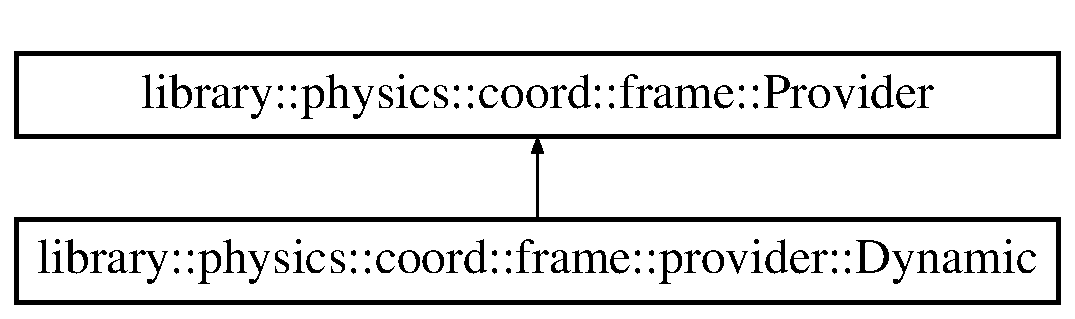
\includegraphics[height=2.000000cm]{classlibrary_1_1physics_1_1coord_1_1frame_1_1provider_1_1_dynamic}
\end{center}
\end{figure}
\subsection*{Public Types}
\begin{DoxyCompactItemize}
\item 
typedef std\+::function$<$ \hyperlink{classlibrary_1_1physics_1_1coord_1_1_transform}{Transform}(const \hyperlink{classlibrary_1_1physics_1_1time_1_1_instant}{Instant} \&)$>$ \hyperlink{classlibrary_1_1physics_1_1coord_1_1frame_1_1provider_1_1_dynamic_a143db93d5b57faf0e91a812f4203a630}{Generator}
\end{DoxyCompactItemize}
\subsection*{Public Member Functions}
\begin{DoxyCompactItemize}
\item 
\hyperlink{classlibrary_1_1physics_1_1coord_1_1frame_1_1provider_1_1_dynamic_a9969003390848043b95d6ee4f451eade}{Dynamic} (const \hyperlink{classlibrary_1_1physics_1_1coord_1_1frame_1_1provider_1_1_dynamic_a143db93d5b57faf0e91a812f4203a630}{Dynamic\+::\+Generator} \&a\+Generator)
\item 
virtual \hyperlink{classlibrary_1_1physics_1_1coord_1_1frame_1_1provider_1_1_dynamic_abca1b794d3c6a306fcbc1eef091330b7}{$\sim$\+Dynamic} () override
\item 
virtual \hyperlink{classlibrary_1_1physics_1_1coord_1_1frame_1_1provider_1_1_dynamic}{Dynamic} $\ast$ \hyperlink{classlibrary_1_1physics_1_1coord_1_1frame_1_1provider_1_1_dynamic_a9d1c9b905420f026fa2f9c26305e47fd}{clone} () const override
\item 
virtual bool \hyperlink{classlibrary_1_1physics_1_1coord_1_1frame_1_1provider_1_1_dynamic_a0527b3fd86cdd8070f1697c057f06479}{is\+Defined} () const override
\item 
virtual \hyperlink{classlibrary_1_1physics_1_1coord_1_1_transform}{Transform} \hyperlink{classlibrary_1_1physics_1_1coord_1_1frame_1_1provider_1_1_dynamic_af9d9f53d8269f24b6694494e5128f11e}{get\+Transform\+At} (const \hyperlink{classlibrary_1_1physics_1_1time_1_1_instant}{Instant} \&an\+Instant) const override
\end{DoxyCompactItemize}
\subsection*{Static Public Member Functions}
\begin{DoxyCompactItemize}
\item 
static \hyperlink{classlibrary_1_1physics_1_1coord_1_1frame_1_1provider_1_1_dynamic}{Dynamic} \hyperlink{classlibrary_1_1physics_1_1coord_1_1frame_1_1provider_1_1_dynamic_a1784249ac5b9abb8562316940998aa2e}{Undefined} ()
\end{DoxyCompactItemize}


\subsection{Detailed Description}
\hyperlink{classlibrary_1_1physics_1_1coord_1_1frame_1_1provider_1_1_dynamic}{Dynamic} provider. 

\subsection{Member Typedef Documentation}
\mbox{\Hypertarget{classlibrary_1_1physics_1_1coord_1_1frame_1_1provider_1_1_dynamic_a143db93d5b57faf0e91a812f4203a630}\label{classlibrary_1_1physics_1_1coord_1_1frame_1_1provider_1_1_dynamic_a143db93d5b57faf0e91a812f4203a630}} 
\index{library\+::physics\+::coord\+::frame\+::provider\+::\+Dynamic@{library\+::physics\+::coord\+::frame\+::provider\+::\+Dynamic}!Generator@{Generator}}
\index{Generator@{Generator}!library\+::physics\+::coord\+::frame\+::provider\+::\+Dynamic@{library\+::physics\+::coord\+::frame\+::provider\+::\+Dynamic}}
\subsubsection{\texorpdfstring{Generator}{Generator}}
{\footnotesize\ttfamily typedef std\+::function$<$\hyperlink{classlibrary_1_1physics_1_1coord_1_1_transform}{Transform} (const \hyperlink{classlibrary_1_1physics_1_1time_1_1_instant}{Instant}\&)$>$ \hyperlink{classlibrary_1_1physics_1_1coord_1_1frame_1_1provider_1_1_dynamic_a143db93d5b57faf0e91a812f4203a630}{library\+::physics\+::coord\+::frame\+::provider\+::\+Dynamic\+::\+Generator}}



\subsection{Constructor \& Destructor Documentation}
\mbox{\Hypertarget{classlibrary_1_1physics_1_1coord_1_1frame_1_1provider_1_1_dynamic_a9969003390848043b95d6ee4f451eade}\label{classlibrary_1_1physics_1_1coord_1_1frame_1_1provider_1_1_dynamic_a9969003390848043b95d6ee4f451eade}} 
\index{library\+::physics\+::coord\+::frame\+::provider\+::\+Dynamic@{library\+::physics\+::coord\+::frame\+::provider\+::\+Dynamic}!Dynamic@{Dynamic}}
\index{Dynamic@{Dynamic}!library\+::physics\+::coord\+::frame\+::provider\+::\+Dynamic@{library\+::physics\+::coord\+::frame\+::provider\+::\+Dynamic}}
\subsubsection{\texorpdfstring{Dynamic()}{Dynamic()}}
{\footnotesize\ttfamily library\+::physics\+::coord\+::frame\+::provider\+::\+Dynamic\+::\+Dynamic (\begin{DoxyParamCaption}\item[{const \hyperlink{classlibrary_1_1physics_1_1coord_1_1frame_1_1provider_1_1_dynamic_a143db93d5b57faf0e91a812f4203a630}{Dynamic\+::\+Generator} \&}]{a\+Generator }\end{DoxyParamCaption})}

\mbox{\Hypertarget{classlibrary_1_1physics_1_1coord_1_1frame_1_1provider_1_1_dynamic_abca1b794d3c6a306fcbc1eef091330b7}\label{classlibrary_1_1physics_1_1coord_1_1frame_1_1provider_1_1_dynamic_abca1b794d3c6a306fcbc1eef091330b7}} 
\index{library\+::physics\+::coord\+::frame\+::provider\+::\+Dynamic@{library\+::physics\+::coord\+::frame\+::provider\+::\+Dynamic}!````~Dynamic@{$\sim$\+Dynamic}}
\index{````~Dynamic@{$\sim$\+Dynamic}!library\+::physics\+::coord\+::frame\+::provider\+::\+Dynamic@{library\+::physics\+::coord\+::frame\+::provider\+::\+Dynamic}}
\subsubsection{\texorpdfstring{$\sim$\+Dynamic()}{~Dynamic()}}
{\footnotesize\ttfamily library\+::physics\+::coord\+::frame\+::provider\+::\+Dynamic\+::$\sim$\+Dynamic (\begin{DoxyParamCaption}{ }\end{DoxyParamCaption})\hspace{0.3cm}{\ttfamily [override]}, {\ttfamily [virtual]}}



\subsection{Member Function Documentation}
\mbox{\Hypertarget{classlibrary_1_1physics_1_1coord_1_1frame_1_1provider_1_1_dynamic_a9d1c9b905420f026fa2f9c26305e47fd}\label{classlibrary_1_1physics_1_1coord_1_1frame_1_1provider_1_1_dynamic_a9d1c9b905420f026fa2f9c26305e47fd}} 
\index{library\+::physics\+::coord\+::frame\+::provider\+::\+Dynamic@{library\+::physics\+::coord\+::frame\+::provider\+::\+Dynamic}!clone@{clone}}
\index{clone@{clone}!library\+::physics\+::coord\+::frame\+::provider\+::\+Dynamic@{library\+::physics\+::coord\+::frame\+::provider\+::\+Dynamic}}
\subsubsection{\texorpdfstring{clone()}{clone()}}
{\footnotesize\ttfamily \hyperlink{classlibrary_1_1physics_1_1coord_1_1frame_1_1provider_1_1_dynamic}{Dynamic} $\ast$ library\+::physics\+::coord\+::frame\+::provider\+::\+Dynamic\+::clone (\begin{DoxyParamCaption}{ }\end{DoxyParamCaption}) const\hspace{0.3cm}{\ttfamily [override]}, {\ttfamily [virtual]}}



Implements \hyperlink{classlibrary_1_1physics_1_1coord_1_1frame_1_1_provider_ab8eee40c8ef4aee0b57bedf458f4934e}{library\+::physics\+::coord\+::frame\+::\+Provider}.

\mbox{\Hypertarget{classlibrary_1_1physics_1_1coord_1_1frame_1_1provider_1_1_dynamic_af9d9f53d8269f24b6694494e5128f11e}\label{classlibrary_1_1physics_1_1coord_1_1frame_1_1provider_1_1_dynamic_af9d9f53d8269f24b6694494e5128f11e}} 
\index{library\+::physics\+::coord\+::frame\+::provider\+::\+Dynamic@{library\+::physics\+::coord\+::frame\+::provider\+::\+Dynamic}!get\+Transform\+At@{get\+Transform\+At}}
\index{get\+Transform\+At@{get\+Transform\+At}!library\+::physics\+::coord\+::frame\+::provider\+::\+Dynamic@{library\+::physics\+::coord\+::frame\+::provider\+::\+Dynamic}}
\subsubsection{\texorpdfstring{get\+Transform\+At()}{getTransformAt()}}
{\footnotesize\ttfamily \hyperlink{classlibrary_1_1physics_1_1coord_1_1_transform}{Transform} library\+::physics\+::coord\+::frame\+::provider\+::\+Dynamic\+::get\+Transform\+At (\begin{DoxyParamCaption}\item[{const \hyperlink{classlibrary_1_1physics_1_1time_1_1_instant}{Instant} \&}]{an\+Instant }\end{DoxyParamCaption}) const\hspace{0.3cm}{\ttfamily [override]}, {\ttfamily [virtual]}}



Implements \hyperlink{classlibrary_1_1physics_1_1coord_1_1frame_1_1_provider_a796fd2dd337f1304a0e9acf573ce2550}{library\+::physics\+::coord\+::frame\+::\+Provider}.

\mbox{\Hypertarget{classlibrary_1_1physics_1_1coord_1_1frame_1_1provider_1_1_dynamic_a0527b3fd86cdd8070f1697c057f06479}\label{classlibrary_1_1physics_1_1coord_1_1frame_1_1provider_1_1_dynamic_a0527b3fd86cdd8070f1697c057f06479}} 
\index{library\+::physics\+::coord\+::frame\+::provider\+::\+Dynamic@{library\+::physics\+::coord\+::frame\+::provider\+::\+Dynamic}!is\+Defined@{is\+Defined}}
\index{is\+Defined@{is\+Defined}!library\+::physics\+::coord\+::frame\+::provider\+::\+Dynamic@{library\+::physics\+::coord\+::frame\+::provider\+::\+Dynamic}}
\subsubsection{\texorpdfstring{is\+Defined()}{isDefined()}}
{\footnotesize\ttfamily bool library\+::physics\+::coord\+::frame\+::provider\+::\+Dynamic\+::is\+Defined (\begin{DoxyParamCaption}{ }\end{DoxyParamCaption}) const\hspace{0.3cm}{\ttfamily [override]}, {\ttfamily [virtual]}}



Implements \hyperlink{classlibrary_1_1physics_1_1coord_1_1frame_1_1_provider_ae7cd093febf2b20f71400f9f79442774}{library\+::physics\+::coord\+::frame\+::\+Provider}.

\mbox{\Hypertarget{classlibrary_1_1physics_1_1coord_1_1frame_1_1provider_1_1_dynamic_a1784249ac5b9abb8562316940998aa2e}\label{classlibrary_1_1physics_1_1coord_1_1frame_1_1provider_1_1_dynamic_a1784249ac5b9abb8562316940998aa2e}} 
\index{library\+::physics\+::coord\+::frame\+::provider\+::\+Dynamic@{library\+::physics\+::coord\+::frame\+::provider\+::\+Dynamic}!Undefined@{Undefined}}
\index{Undefined@{Undefined}!library\+::physics\+::coord\+::frame\+::provider\+::\+Dynamic@{library\+::physics\+::coord\+::frame\+::provider\+::\+Dynamic}}
\subsubsection{\texorpdfstring{Undefined()}{Undefined()}}
{\footnotesize\ttfamily \hyperlink{classlibrary_1_1physics_1_1coord_1_1frame_1_1provider_1_1_dynamic}{Dynamic} library\+::physics\+::coord\+::frame\+::provider\+::\+Dynamic\+::\+Undefined (\begin{DoxyParamCaption}{ }\end{DoxyParamCaption})\hspace{0.3cm}{\ttfamily [static]}}



The documentation for this class was generated from the following files\+:\begin{DoxyCompactItemize}
\item 
include/\+Library/\+Physics/\+Coordinate/\+Frame/\+Providers/\hyperlink{_dynamic_8hpp}{Dynamic.\+hpp}\item 
src/\+Library/\+Physics/\+Coordinate/\+Frame/\+Providers/\hyperlink{_dynamic_8cpp}{Dynamic.\+cpp}\end{DoxyCompactItemize}

\hypertarget{classlibrary_1_1physics_1_1env_1_1obj_1_1celest_1_1_earth}{}\section{library\+:\+:physics\+:\+:env\+:\+:obj\+:\+:celest\+:\+:Earth Class Reference}
\label{classlibrary_1_1physics_1_1env_1_1obj_1_1celest_1_1_earth}\index{library\+::physics\+::env\+::obj\+::celest\+::\+Earth@{library\+::physics\+::env\+::obj\+::celest\+::\+Earth}}


{\ttfamily \#include $<$Earth.\+hpp$>$}

Inheritance diagram for library\+:\+:physics\+:\+:env\+:\+:obj\+:\+:celest\+:\+:Earth\+:\begin{figure}[H]
\begin{center}
\leavevmode
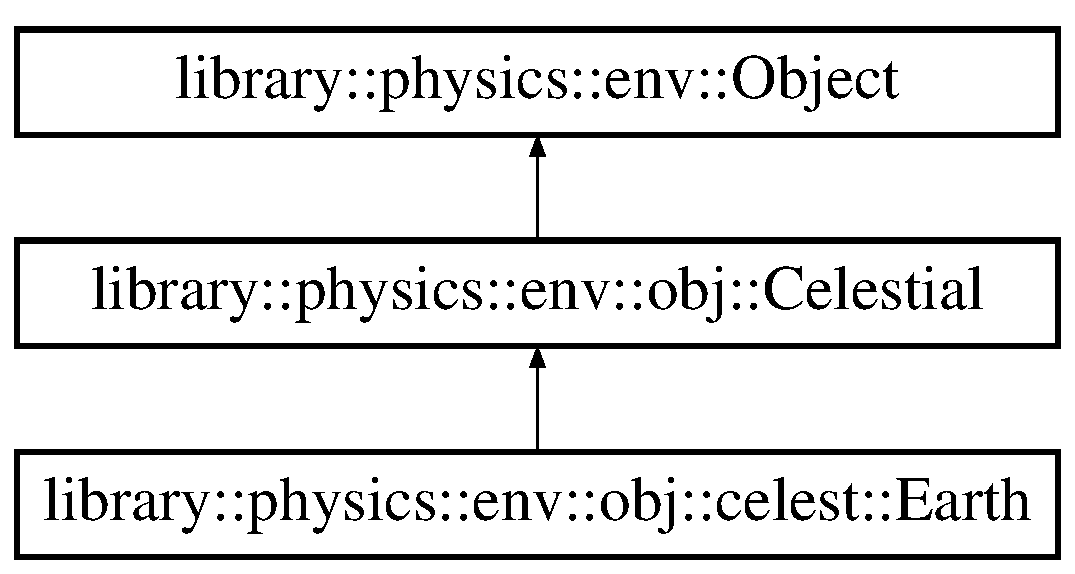
\includegraphics[height=3.000000cm]{classlibrary_1_1physics_1_1env_1_1obj_1_1celest_1_1_earth}
\end{center}
\end{figure}
\subsection*{Public Member Functions}
\begin{DoxyCompactItemize}
\item 
\hyperlink{classlibrary_1_1physics_1_1env_1_1obj_1_1celest_1_1_earth_a775057b64077c61329a426260327022c}{Earth} (const Shared$<$ \hyperlink{classlibrary_1_1physics_1_1env_1_1_ephemeris}{Ephemeris} $>$ \&an\+Ephemeris\+S\+Ptr, const \hyperlink{classlibrary_1_1physics_1_1time_1_1_instant}{Instant} \&an\+Instant)
\item 
virtual \hyperlink{classlibrary_1_1physics_1_1env_1_1obj_1_1celest_1_1_earth_a93fbd2015a7c7d786654919197c63963}{$\sim$\+Earth} () override
\item 
virtual \hyperlink{classlibrary_1_1physics_1_1env_1_1obj_1_1celest_1_1_earth}{Earth} $\ast$ \hyperlink{classlibrary_1_1physics_1_1env_1_1obj_1_1celest_1_1_earth_aca39bec00a2046a3fcef9bf22be52428}{clone} () const override
\end{DoxyCompactItemize}
\subsection*{Static Public Member Functions}
\begin{DoxyCompactItemize}
\item 
static \hyperlink{classlibrary_1_1physics_1_1env_1_1obj_1_1celest_1_1_earth}{Earth} \hyperlink{classlibrary_1_1physics_1_1env_1_1obj_1_1celest_1_1_earth_af0456d0dfe17d3cf4473ec02aec1683b}{Analytical} (const \hyperlink{classlibrary_1_1physics_1_1time_1_1_instant}{Instant} \&an\+Instant=\hyperlink{classlibrary_1_1physics_1_1time_1_1_instant_a2a4f57aa71693b8def06788d55bc3bd3}{Instant\+::\+J2000}())
\end{DoxyCompactItemize}
\subsection*{Static Public Attributes}
\begin{DoxyCompactItemize}
\item 
static \hyperlink{classlibrary_1_1physics_1_1units_1_1_derived}{Derived} \hyperlink{classlibrary_1_1physics_1_1env_1_1obj_1_1celest_1_1_earth_a3375ee38a895b234ca2c91e1de4f2baa}{Gravitational\+Constant} = \hyperlink{classlibrary_1_1physics_1_1units_1_1_derived}{Derived}(398600441500000.\+0, \{ \hyperlink{classlibrary_1_1physics_1_1units_1_1_length_a3b8b39cd245cf6b19dc34459baeccb18a17c9c40b9db5a0983d1075a012c1f90a}{Length\+::\+Unit\+::\+Meter}, \hyperlink{classlibrary_1_1physics_1_1units_1_1_derived_1_1_order}{Derived\+::\+Order}(3), \hyperlink{classlibrary_1_1physics_1_1units_1_1_mass_a95f1e0434bc16794926b8e273bc2a54baec0fc0100c4fc1ce4eea230c3dc10360}{Mass\+::\+Unit\+::\+Undefined}, \hyperlink{classlibrary_1_1physics_1_1units_1_1_derived_1_1_order_ad001256340bff8a9c55156f9c45d4969}{Derived\+::\+Order\+::\+Zero}(), \hyperlink{classlibrary_1_1physics_1_1units_1_1_time_ab876a6a05c9a2f28905f2753bfd64109ac22cf8376b1893dcfcef0649fe1a7d87}{Time\+::\+Unit\+::\+Second}, \hyperlink{classlibrary_1_1physics_1_1units_1_1_derived_1_1_order}{Derived\+::\+Order}(-\/2), \hyperlink{classlibrary_1_1physics_1_1units_1_1_angle_a3c329d415a61783b16ce481874cc5956aec0fc0100c4fc1ce4eea230c3dc10360}{Angle\+::\+Unit\+::\+Undefined}, \hyperlink{classlibrary_1_1physics_1_1units_1_1_derived_1_1_order_ad001256340bff8a9c55156f9c45d4969}{Derived\+::\+Order\+::\+Zero}() \})
\item 
static \hyperlink{classlibrary_1_1physics_1_1units_1_1_length}{Length} \hyperlink{classlibrary_1_1physics_1_1env_1_1obj_1_1celest_1_1_earth_a1f7b0ecdcec2f807427923af8d0d87dd}{Equatorial\+Radius} = \hyperlink{classlibrary_1_1physics_1_1units_1_1_length_ad523a3737d5c3f23a64588eac83f2148}{Length\+::\+Meters}(6378136.\+3)
\item 
static Real \hyperlink{classlibrary_1_1physics_1_1env_1_1obj_1_1celest_1_1_earth_ac456fb7204d40826b62a73a59b55176b}{Flattening} = 0.\+003352810664747
\item 
static Real \hyperlink{classlibrary_1_1physics_1_1env_1_1obj_1_1celest_1_1_earth_a0acd5f5fe99a0aacc7175fe0a140360f}{C20} = -\/4.\+841653717360e-\/04
\item 
static Real \hyperlink{classlibrary_1_1physics_1_1env_1_1obj_1_1celest_1_1_earth_a45eb6624c62b847e0f2c59f7b6a7aad5}{J2} = -\/\hyperlink{classlibrary_1_1physics_1_1env_1_1obj_1_1celest_1_1_earth_a0acd5f5fe99a0aacc7175fe0a140360f}{Earth\+::\+C20} $\ast$ std\+::sqrt(5.\+0)
\end{DoxyCompactItemize}
\subsection*{Additional Inherited Members}


\subsection{Constructor \& Destructor Documentation}
\mbox{\Hypertarget{classlibrary_1_1physics_1_1env_1_1obj_1_1celest_1_1_earth_a775057b64077c61329a426260327022c}\label{classlibrary_1_1physics_1_1env_1_1obj_1_1celest_1_1_earth_a775057b64077c61329a426260327022c}} 
\index{library\+::physics\+::env\+::obj\+::celest\+::\+Earth@{library\+::physics\+::env\+::obj\+::celest\+::\+Earth}!Earth@{Earth}}
\index{Earth@{Earth}!library\+::physics\+::env\+::obj\+::celest\+::\+Earth@{library\+::physics\+::env\+::obj\+::celest\+::\+Earth}}
\subsubsection{\texorpdfstring{Earth()}{Earth()}}
{\footnotesize\ttfamily library\+::physics\+::env\+::obj\+::celest\+::\+Earth\+::\+Earth (\begin{DoxyParamCaption}\item[{const Shared$<$ \hyperlink{classlibrary_1_1physics_1_1env_1_1_ephemeris}{Ephemeris} $>$ \&}]{an\+Ephemeris\+S\+Ptr,  }\item[{const \hyperlink{classlibrary_1_1physics_1_1time_1_1_instant}{Instant} \&}]{an\+Instant }\end{DoxyParamCaption})}

\mbox{\Hypertarget{classlibrary_1_1physics_1_1env_1_1obj_1_1celest_1_1_earth_a93fbd2015a7c7d786654919197c63963}\label{classlibrary_1_1physics_1_1env_1_1obj_1_1celest_1_1_earth_a93fbd2015a7c7d786654919197c63963}} 
\index{library\+::physics\+::env\+::obj\+::celest\+::\+Earth@{library\+::physics\+::env\+::obj\+::celest\+::\+Earth}!````~Earth@{$\sim$\+Earth}}
\index{````~Earth@{$\sim$\+Earth}!library\+::physics\+::env\+::obj\+::celest\+::\+Earth@{library\+::physics\+::env\+::obj\+::celest\+::\+Earth}}
\subsubsection{\texorpdfstring{$\sim$\+Earth()}{~Earth()}}
{\footnotesize\ttfamily library\+::physics\+::env\+::obj\+::celest\+::\+Earth\+::$\sim$\+Earth (\begin{DoxyParamCaption}{ }\end{DoxyParamCaption})\hspace{0.3cm}{\ttfamily [override]}, {\ttfamily [virtual]}}



\subsection{Member Function Documentation}
\mbox{\Hypertarget{classlibrary_1_1physics_1_1env_1_1obj_1_1celest_1_1_earth_af0456d0dfe17d3cf4473ec02aec1683b}\label{classlibrary_1_1physics_1_1env_1_1obj_1_1celest_1_1_earth_af0456d0dfe17d3cf4473ec02aec1683b}} 
\index{library\+::physics\+::env\+::obj\+::celest\+::\+Earth@{library\+::physics\+::env\+::obj\+::celest\+::\+Earth}!Analytical@{Analytical}}
\index{Analytical@{Analytical}!library\+::physics\+::env\+::obj\+::celest\+::\+Earth@{library\+::physics\+::env\+::obj\+::celest\+::\+Earth}}
\subsubsection{\texorpdfstring{Analytical()}{Analytical()}}
{\footnotesize\ttfamily \hyperlink{classlibrary_1_1physics_1_1env_1_1obj_1_1celest_1_1_earth}{Earth} library\+::physics\+::env\+::obj\+::celest\+::\+Earth\+::\+Analytical (\begin{DoxyParamCaption}\item[{const \hyperlink{classlibrary_1_1physics_1_1time_1_1_instant}{Instant} \&}]{an\+Instant = {\ttfamily \hyperlink{classlibrary_1_1physics_1_1time_1_1_instant_a2a4f57aa71693b8def06788d55bc3bd3}{Instant\+::\+J2000}()} }\end{DoxyParamCaption})\hspace{0.3cm}{\ttfamily [static]}}

\mbox{\Hypertarget{classlibrary_1_1physics_1_1env_1_1obj_1_1celest_1_1_earth_aca39bec00a2046a3fcef9bf22be52428}\label{classlibrary_1_1physics_1_1env_1_1obj_1_1celest_1_1_earth_aca39bec00a2046a3fcef9bf22be52428}} 
\index{library\+::physics\+::env\+::obj\+::celest\+::\+Earth@{library\+::physics\+::env\+::obj\+::celest\+::\+Earth}!clone@{clone}}
\index{clone@{clone}!library\+::physics\+::env\+::obj\+::celest\+::\+Earth@{library\+::physics\+::env\+::obj\+::celest\+::\+Earth}}
\subsubsection{\texorpdfstring{clone()}{clone()}}
{\footnotesize\ttfamily \hyperlink{classlibrary_1_1physics_1_1env_1_1obj_1_1celest_1_1_earth}{Earth} $\ast$ library\+::physics\+::env\+::obj\+::celest\+::\+Earth\+::clone (\begin{DoxyParamCaption}{ }\end{DoxyParamCaption}) const\hspace{0.3cm}{\ttfamily [override]}, {\ttfamily [virtual]}}



Reimplemented from \hyperlink{classlibrary_1_1physics_1_1env_1_1obj_1_1_celestial_aaf8aa41a0ff9336eba62c07e3c27f82d}{library\+::physics\+::env\+::obj\+::\+Celestial}.



\subsection{Member Data Documentation}
\mbox{\Hypertarget{classlibrary_1_1physics_1_1env_1_1obj_1_1celest_1_1_earth_a0acd5f5fe99a0aacc7175fe0a140360f}\label{classlibrary_1_1physics_1_1env_1_1obj_1_1celest_1_1_earth_a0acd5f5fe99a0aacc7175fe0a140360f}} 
\index{library\+::physics\+::env\+::obj\+::celest\+::\+Earth@{library\+::physics\+::env\+::obj\+::celest\+::\+Earth}!C20@{C20}}
\index{C20@{C20}!library\+::physics\+::env\+::obj\+::celest\+::\+Earth@{library\+::physics\+::env\+::obj\+::celest\+::\+Earth}}
\subsubsection{\texorpdfstring{C20}{C20}}
{\footnotesize\ttfamily Real library\+::physics\+::env\+::obj\+::celest\+::\+Earth\+::\+C20 = -\/4.\+841653717360e-\/04\hspace{0.3cm}{\ttfamily [static]}}

\mbox{\Hypertarget{classlibrary_1_1physics_1_1env_1_1obj_1_1celest_1_1_earth_a1f7b0ecdcec2f807427923af8d0d87dd}\label{classlibrary_1_1physics_1_1env_1_1obj_1_1celest_1_1_earth_a1f7b0ecdcec2f807427923af8d0d87dd}} 
\index{library\+::physics\+::env\+::obj\+::celest\+::\+Earth@{library\+::physics\+::env\+::obj\+::celest\+::\+Earth}!Equatorial\+Radius@{Equatorial\+Radius}}
\index{Equatorial\+Radius@{Equatorial\+Radius}!library\+::physics\+::env\+::obj\+::celest\+::\+Earth@{library\+::physics\+::env\+::obj\+::celest\+::\+Earth}}
\subsubsection{\texorpdfstring{Equatorial\+Radius}{EquatorialRadius}}
{\footnotesize\ttfamily \hyperlink{classlibrary_1_1physics_1_1units_1_1_length}{Length} library\+::physics\+::env\+::obj\+::celest\+::\+Earth\+::\+Equatorial\+Radius = \hyperlink{classlibrary_1_1physics_1_1units_1_1_length_ad523a3737d5c3f23a64588eac83f2148}{Length\+::\+Meters}(6378136.\+3)\hspace{0.3cm}{\ttfamily [static]}}

\mbox{\Hypertarget{classlibrary_1_1physics_1_1env_1_1obj_1_1celest_1_1_earth_ac456fb7204d40826b62a73a59b55176b}\label{classlibrary_1_1physics_1_1env_1_1obj_1_1celest_1_1_earth_ac456fb7204d40826b62a73a59b55176b}} 
\index{library\+::physics\+::env\+::obj\+::celest\+::\+Earth@{library\+::physics\+::env\+::obj\+::celest\+::\+Earth}!Flattening@{Flattening}}
\index{Flattening@{Flattening}!library\+::physics\+::env\+::obj\+::celest\+::\+Earth@{library\+::physics\+::env\+::obj\+::celest\+::\+Earth}}
\subsubsection{\texorpdfstring{Flattening}{Flattening}}
{\footnotesize\ttfamily Real library\+::physics\+::env\+::obj\+::celest\+::\+Earth\+::\+Flattening = 0.\+003352810664747\hspace{0.3cm}{\ttfamily [static]}}

\mbox{\Hypertarget{classlibrary_1_1physics_1_1env_1_1obj_1_1celest_1_1_earth_a3375ee38a895b234ca2c91e1de4f2baa}\label{classlibrary_1_1physics_1_1env_1_1obj_1_1celest_1_1_earth_a3375ee38a895b234ca2c91e1de4f2baa}} 
\index{library\+::physics\+::env\+::obj\+::celest\+::\+Earth@{library\+::physics\+::env\+::obj\+::celest\+::\+Earth}!Gravitational\+Constant@{Gravitational\+Constant}}
\index{Gravitational\+Constant@{Gravitational\+Constant}!library\+::physics\+::env\+::obj\+::celest\+::\+Earth@{library\+::physics\+::env\+::obj\+::celest\+::\+Earth}}
\subsubsection{\texorpdfstring{Gravitational\+Constant}{GravitationalConstant}}
{\footnotesize\ttfamily \hyperlink{classlibrary_1_1physics_1_1units_1_1_derived}{Derived} library\+::physics\+::env\+::obj\+::celest\+::\+Earth\+::\+Gravitational\+Constant = \hyperlink{classlibrary_1_1physics_1_1units_1_1_derived}{Derived}(398600441500000.\+0, \{ \hyperlink{classlibrary_1_1physics_1_1units_1_1_length_a3b8b39cd245cf6b19dc34459baeccb18a17c9c40b9db5a0983d1075a012c1f90a}{Length\+::\+Unit\+::\+Meter}, \hyperlink{classlibrary_1_1physics_1_1units_1_1_derived_1_1_order}{Derived\+::\+Order}(3), \hyperlink{classlibrary_1_1physics_1_1units_1_1_mass_a95f1e0434bc16794926b8e273bc2a54baec0fc0100c4fc1ce4eea230c3dc10360}{Mass\+::\+Unit\+::\+Undefined}, \hyperlink{classlibrary_1_1physics_1_1units_1_1_derived_1_1_order_ad001256340bff8a9c55156f9c45d4969}{Derived\+::\+Order\+::\+Zero}(), \hyperlink{classlibrary_1_1physics_1_1units_1_1_time_ab876a6a05c9a2f28905f2753bfd64109ac22cf8376b1893dcfcef0649fe1a7d87}{Time\+::\+Unit\+::\+Second}, \hyperlink{classlibrary_1_1physics_1_1units_1_1_derived_1_1_order}{Derived\+::\+Order}(-\/2), \hyperlink{classlibrary_1_1physics_1_1units_1_1_angle_a3c329d415a61783b16ce481874cc5956aec0fc0100c4fc1ce4eea230c3dc10360}{Angle\+::\+Unit\+::\+Undefined}, \hyperlink{classlibrary_1_1physics_1_1units_1_1_derived_1_1_order_ad001256340bff8a9c55156f9c45d4969}{Derived\+::\+Order\+::\+Zero}() \})\hspace{0.3cm}{\ttfamily [static]}}

\mbox{\Hypertarget{classlibrary_1_1physics_1_1env_1_1obj_1_1celest_1_1_earth_a45eb6624c62b847e0f2c59f7b6a7aad5}\label{classlibrary_1_1physics_1_1env_1_1obj_1_1celest_1_1_earth_a45eb6624c62b847e0f2c59f7b6a7aad5}} 
\index{library\+::physics\+::env\+::obj\+::celest\+::\+Earth@{library\+::physics\+::env\+::obj\+::celest\+::\+Earth}!J2@{J2}}
\index{J2@{J2}!library\+::physics\+::env\+::obj\+::celest\+::\+Earth@{library\+::physics\+::env\+::obj\+::celest\+::\+Earth}}
\subsubsection{\texorpdfstring{J2}{J2}}
{\footnotesize\ttfamily Real library\+::physics\+::env\+::obj\+::celest\+::\+Earth\+::\+J2 = -\/\hyperlink{classlibrary_1_1physics_1_1env_1_1obj_1_1celest_1_1_earth_a0acd5f5fe99a0aacc7175fe0a140360f}{Earth\+::\+C20} $\ast$ std\+::sqrt(5.\+0)\hspace{0.3cm}{\ttfamily [static]}}



The documentation for this class was generated from the following files\+:\begin{DoxyCompactItemize}
\item 
include/\+Library/\+Physics/\+Environment/\+Objects/\+Celestial\+Bodies/\hyperlink{_earth_8hpp}{Earth.\+hpp}\item 
src/\+Library/\+Physics/\+Environment/\+Objects/\+Celestial\+Bodies/\hyperlink{_earth_8cpp}{Earth.\+cpp}\end{DoxyCompactItemize}

\hypertarget{classlibrary_1_1physics_1_1env_1_1ephem_1_1spice_1_1_engine}{}\section{library\+:\+:physics\+:\+:env\+:\+:ephem\+:\+:spice\+:\+:Engine Class Reference}
\label{classlibrary_1_1physics_1_1env_1_1ephem_1_1spice_1_1_engine}\index{library\+::physics\+::env\+::ephem\+::spice\+::\+Engine@{library\+::physics\+::env\+::ephem\+::spice\+::\+Engine}}


\hyperlink{classlibrary_1_1physics_1_1env_1_1ephem_1_1_s_p_i_c_e}{S\+P\+I\+CE} Toolkit engine.  




{\ttfamily \#include $<$Engine.\+hpp$>$}

\subsection*{Public Member Functions}
\begin{DoxyCompactItemize}
\item 
\hyperlink{classlibrary_1_1physics_1_1env_1_1ephem_1_1spice_1_1_engine_a26bf9260d2730a6825a975c1a0b49b5b}{Engine} (const \hyperlink{classlibrary_1_1physics_1_1env_1_1ephem_1_1spice_1_1_engine}{Engine} \&a\+Spice\+Engine)=delete
\item 
\hyperlink{classlibrary_1_1physics_1_1env_1_1ephem_1_1spice_1_1_engine}{Engine} \& \hyperlink{classlibrary_1_1physics_1_1env_1_1ephem_1_1spice_1_1_engine_a6aca23c8962df540725dc0e9fbb3eb47}{operator=} (const \hyperlink{classlibrary_1_1physics_1_1env_1_1ephem_1_1spice_1_1_engine}{Engine} \&a\+Spice\+Engine)=delete
\item 
Shared$<$ const \hyperlink{classlibrary_1_1physics_1_1coord_1_1_frame}{Frame} $>$ \hyperlink{classlibrary_1_1physics_1_1env_1_1ephem_1_1spice_1_1_engine_af5bdad7a3783f772b726ac3f0cd09957}{get\+Frame\+Of} (const \hyperlink{classlibrary_1_1physics_1_1env_1_1ephem_1_1_s_p_i_c_e_a86f1a863677210ba8884807cc725c0f8}{S\+P\+I\+C\+E\+::\+Object} \&a\+Spice\+Object) const
\item 
void \hyperlink{classlibrary_1_1physics_1_1env_1_1ephem_1_1spice_1_1_engine_ada61913070593a15e7417ad300ae67d2}{load\+Kernel} (const File \&a\+Kernel\+File)
\end{DoxyCompactItemize}
\subsection*{Static Public Member Functions}
\begin{DoxyCompactItemize}
\item 
static \hyperlink{classlibrary_1_1physics_1_1env_1_1ephem_1_1spice_1_1_engine}{Engine} \& \hyperlink{classlibrary_1_1physics_1_1env_1_1ephem_1_1spice_1_1_engine_a9d5058448b12c353edcf5a420cec2745}{Get} ()
\end{DoxyCompactItemize}


\subsection{Detailed Description}
\hyperlink{classlibrary_1_1physics_1_1env_1_1ephem_1_1_s_p_i_c_e}{S\+P\+I\+CE} Toolkit engine. 

\subsection{Constructor \& Destructor Documentation}
\mbox{\Hypertarget{classlibrary_1_1physics_1_1env_1_1ephem_1_1spice_1_1_engine_a26bf9260d2730a6825a975c1a0b49b5b}\label{classlibrary_1_1physics_1_1env_1_1ephem_1_1spice_1_1_engine_a26bf9260d2730a6825a975c1a0b49b5b}} 
\index{library\+::physics\+::env\+::ephem\+::spice\+::\+Engine@{library\+::physics\+::env\+::ephem\+::spice\+::\+Engine}!Engine@{Engine}}
\index{Engine@{Engine}!library\+::physics\+::env\+::ephem\+::spice\+::\+Engine@{library\+::physics\+::env\+::ephem\+::spice\+::\+Engine}}
\subsubsection{\texorpdfstring{Engine()}{Engine()}}
{\footnotesize\ttfamily library\+::physics\+::env\+::ephem\+::spice\+::\+Engine\+::\+Engine (\begin{DoxyParamCaption}\item[{const \hyperlink{classlibrary_1_1physics_1_1env_1_1ephem_1_1spice_1_1_engine}{Engine} \&}]{a\+Spice\+Engine }\end{DoxyParamCaption})\hspace{0.3cm}{\ttfamily [delete]}}



\subsection{Member Function Documentation}
\mbox{\Hypertarget{classlibrary_1_1physics_1_1env_1_1ephem_1_1spice_1_1_engine_a9d5058448b12c353edcf5a420cec2745}\label{classlibrary_1_1physics_1_1env_1_1ephem_1_1spice_1_1_engine_a9d5058448b12c353edcf5a420cec2745}} 
\index{library\+::physics\+::env\+::ephem\+::spice\+::\+Engine@{library\+::physics\+::env\+::ephem\+::spice\+::\+Engine}!Get@{Get}}
\index{Get@{Get}!library\+::physics\+::env\+::ephem\+::spice\+::\+Engine@{library\+::physics\+::env\+::ephem\+::spice\+::\+Engine}}
\subsubsection{\texorpdfstring{Get()}{Get()}}
{\footnotesize\ttfamily \hyperlink{classlibrary_1_1physics_1_1env_1_1ephem_1_1spice_1_1_engine}{Engine} \& library\+::physics\+::env\+::ephem\+::spice\+::\+Engine\+::\+Get (\begin{DoxyParamCaption}{ }\end{DoxyParamCaption})\hspace{0.3cm}{\ttfamily [static]}}

\mbox{\Hypertarget{classlibrary_1_1physics_1_1env_1_1ephem_1_1spice_1_1_engine_af5bdad7a3783f772b726ac3f0cd09957}\label{classlibrary_1_1physics_1_1env_1_1ephem_1_1spice_1_1_engine_af5bdad7a3783f772b726ac3f0cd09957}} 
\index{library\+::physics\+::env\+::ephem\+::spice\+::\+Engine@{library\+::physics\+::env\+::ephem\+::spice\+::\+Engine}!get\+Frame\+Of@{get\+Frame\+Of}}
\index{get\+Frame\+Of@{get\+Frame\+Of}!library\+::physics\+::env\+::ephem\+::spice\+::\+Engine@{library\+::physics\+::env\+::ephem\+::spice\+::\+Engine}}
\subsubsection{\texorpdfstring{get\+Frame\+Of()}{getFrameOf()}}
{\footnotesize\ttfamily Shared$<$ const \hyperlink{classlibrary_1_1physics_1_1coord_1_1_frame}{Frame} $>$ library\+::physics\+::env\+::ephem\+::spice\+::\+Engine\+::get\+Frame\+Of (\begin{DoxyParamCaption}\item[{const \hyperlink{classlibrary_1_1physics_1_1env_1_1ephem_1_1_s_p_i_c_e_a86f1a863677210ba8884807cc725c0f8}{S\+P\+I\+C\+E\+::\+Object} \&}]{a\+Spice\+Object }\end{DoxyParamCaption}) const}

\mbox{\Hypertarget{classlibrary_1_1physics_1_1env_1_1ephem_1_1spice_1_1_engine_ada61913070593a15e7417ad300ae67d2}\label{classlibrary_1_1physics_1_1env_1_1ephem_1_1spice_1_1_engine_ada61913070593a15e7417ad300ae67d2}} 
\index{library\+::physics\+::env\+::ephem\+::spice\+::\+Engine@{library\+::physics\+::env\+::ephem\+::spice\+::\+Engine}!load\+Kernel@{load\+Kernel}}
\index{load\+Kernel@{load\+Kernel}!library\+::physics\+::env\+::ephem\+::spice\+::\+Engine@{library\+::physics\+::env\+::ephem\+::spice\+::\+Engine}}
\subsubsection{\texorpdfstring{load\+Kernel()}{loadKernel()}}
{\footnotesize\ttfamily void library\+::physics\+::env\+::ephem\+::spice\+::\+Engine\+::load\+Kernel (\begin{DoxyParamCaption}\item[{const File \&}]{a\+Kernel\+File }\end{DoxyParamCaption})}

\mbox{\Hypertarget{classlibrary_1_1physics_1_1env_1_1ephem_1_1spice_1_1_engine_a6aca23c8962df540725dc0e9fbb3eb47}\label{classlibrary_1_1physics_1_1env_1_1ephem_1_1spice_1_1_engine_a6aca23c8962df540725dc0e9fbb3eb47}} 
\index{library\+::physics\+::env\+::ephem\+::spice\+::\+Engine@{library\+::physics\+::env\+::ephem\+::spice\+::\+Engine}!operator=@{operator=}}
\index{operator=@{operator=}!library\+::physics\+::env\+::ephem\+::spice\+::\+Engine@{library\+::physics\+::env\+::ephem\+::spice\+::\+Engine}}
\subsubsection{\texorpdfstring{operator=()}{operator=()}}
{\footnotesize\ttfamily \hyperlink{classlibrary_1_1physics_1_1env_1_1ephem_1_1spice_1_1_engine}{Engine}\& library\+::physics\+::env\+::ephem\+::spice\+::\+Engine\+::operator= (\begin{DoxyParamCaption}\item[{const \hyperlink{classlibrary_1_1physics_1_1env_1_1ephem_1_1spice_1_1_engine}{Engine} \&}]{a\+Spice\+Engine }\end{DoxyParamCaption})\hspace{0.3cm}{\ttfamily [delete]}}



The documentation for this class was generated from the following files\+:\begin{DoxyCompactItemize}
\item 
include/\+Library/\+Physics/\+Environment/\+Ephemerides/\+S\+P\+I\+C\+E/\hyperlink{_engine_8hpp}{Engine.\+hpp}\item 
src/\+Library/\+Physics/\+Environment/\+Ephemerides/\+S\+P\+I\+C\+E/\hyperlink{_engine_8cpp}{Engine.\+cpp}\end{DoxyCompactItemize}

\hypertarget{classlibrary_1_1physics_1_1_environment}{}\section{library\+:\+:physics\+:\+:Environment Class Reference}
\label{classlibrary_1_1physics_1_1_environment}\index{library\+::physics\+::\+Environment@{library\+::physics\+::\+Environment}}


\hyperlink{classlibrary_1_1physics_1_1_environment}{Environment} modeling.  




{\ttfamily \#include $<$Environment.\+hpp$>$}

\subsection*{Public Member Functions}
\begin{DoxyCompactItemize}
\item 
\hyperlink{classlibrary_1_1physics_1_1_environment_a51854f130c31eb075ea623e332978495}{Environment} (const \hyperlink{classlibrary_1_1physics_1_1time_1_1_instant}{Instant} \&an\+Instant, const Array$<$ Shared$<$ \hyperlink{classlibrary_1_1physics_1_1env_1_1_object}{Object} $>$$>$ \&an\+Object\+Array)
\begin{DoxyCompactList}\small\item\em Constructor. \end{DoxyCompactList}\item 
\hyperlink{classlibrary_1_1physics_1_1_environment_afb2fe03dcd7061a8ed5e155d7d134ba2}{Environment} (const \hyperlink{classlibrary_1_1physics_1_1_environment}{Environment} \&an\+Environment)
\begin{DoxyCompactList}\small\item\em Copy constructor. \end{DoxyCompactList}\item 
\hyperlink{classlibrary_1_1physics_1_1_environment}{Environment} \& \hyperlink{classlibrary_1_1physics_1_1_environment_a3410b331642161ad087d76b7d5019a86}{operator=} (const \hyperlink{classlibrary_1_1physics_1_1_environment}{Environment} \&an\+Environment)
\begin{DoxyCompactList}\small\item\em Copy assignment operator. \end{DoxyCompactList}\item 
bool \hyperlink{classlibrary_1_1physics_1_1_environment_acbe2e199328ec6a3d2c233dbe8eb6359}{is\+Defined} () const
\begin{DoxyCompactList}\small\item\em Check if environment is defined. \end{DoxyCompactList}\item 
bool \hyperlink{classlibrary_1_1physics_1_1_environment_ab88060948d60e3775d3c48047e1565aa}{has\+Object\+With\+Name} (const String \&a\+Name) const
\begin{DoxyCompactList}\small\item\em Returns true if environment contains objects with a given name. \end{DoxyCompactList}\item 
bool \hyperlink{classlibrary_1_1physics_1_1_environment_a96b2455aff4cefe7d5ce92bb008a7d51}{intersects} (const \hyperlink{classlibrary_1_1physics_1_1env_1_1_object_abdf50733c7ad97327fb64edca5670f13}{Object\+::\+Geometry} \&a\+Geometry) const
\begin{DoxyCompactList}\small\item\em Returns true if a given geometry intersects any of the environment objects. \end{DoxyCompactList}\item 
Array$<$ Shared$<$ const \hyperlink{classlibrary_1_1physics_1_1env_1_1_object}{Object} $>$ $>$ \hyperlink{classlibrary_1_1physics_1_1_environment_a109b7156dadfe992126e01c629146a75}{access\+Objects} () const
\begin{DoxyCompactList}\small\item\em Access objects. \end{DoxyCompactList}\item 
Shared$<$ const \hyperlink{classlibrary_1_1physics_1_1env_1_1_object}{Object} $>$ \hyperlink{classlibrary_1_1physics_1_1_environment_adb18bd17dfbffa181d7e0d868c2647a0}{access\+Object\+With\+Name} (const String \&a\+Name) const
\begin{DoxyCompactList}\small\item\em Access object with a given name. \end{DoxyCompactList}\item 
Shared$<$ const \hyperlink{classlibrary_1_1physics_1_1env_1_1obj_1_1_celestial}{Celestial} $>$ \hyperlink{classlibrary_1_1physics_1_1_environment_a3dd52e151e9f09788d46072095bd48a6}{access\+Celestial\+Object\+With\+Name} (const String \&a\+Name) const
\begin{DoxyCompactList}\small\item\em Access celestial object with a given name. \end{DoxyCompactList}\item 
\hyperlink{classlibrary_1_1physics_1_1time_1_1_instant}{Instant} \hyperlink{classlibrary_1_1physics_1_1_environment_a551ca61eb2aebd762e67b7c9e561d22e}{get\+Instant} () const
\begin{DoxyCompactList}\small\item\em Get instant. \end{DoxyCompactList}\item 
Array$<$ String $>$ \hyperlink{classlibrary_1_1physics_1_1_environment_ad90a5d1e67d62009e7cf6875c4fa7907}{get\+Object\+Names} () const
\begin{DoxyCompactList}\small\item\em Get names of objects. \end{DoxyCompactList}\item 
void \hyperlink{classlibrary_1_1physics_1_1_environment_a6279d44965a3894993cee2bc0c51d068}{set\+Instant} (const \hyperlink{classlibrary_1_1physics_1_1time_1_1_instant}{Instant} \&an\+Instant)
\begin{DoxyCompactList}\small\item\em Set instant. \end{DoxyCompactList}\end{DoxyCompactItemize}
\subsection*{Static Public Member Functions}
\begin{DoxyCompactItemize}
\item 
static \hyperlink{classlibrary_1_1physics_1_1_environment}{Environment} \hyperlink{classlibrary_1_1physics_1_1_environment_a8d1dfff3867d59ecdebd3ee6e98a2dab}{Undefined} ()
\item 
static \hyperlink{classlibrary_1_1physics_1_1_environment}{Environment} \hyperlink{classlibrary_1_1physics_1_1_environment_a7fcc57999bfb9c0c7e70b7cc783e30c8}{Default} ()
\end{DoxyCompactItemize}
\subsection*{Friends}
\begin{DoxyCompactItemize}
\item 
std\+::ostream \& \hyperlink{classlibrary_1_1physics_1_1_environment_a7bc4b39898452fbe5ce3a8de75ad2596}{operator$<$$<$} (std\+::ostream \&an\+Output\+Stream, const \hyperlink{classlibrary_1_1physics_1_1_environment}{Environment} \&an\+Environment)
\begin{DoxyCompactList}\small\item\em Output stream operator. \end{DoxyCompactList}\end{DoxyCompactItemize}


\subsection{Detailed Description}
\hyperlink{classlibrary_1_1physics_1_1_environment}{Environment} modeling. 

\subsection{Constructor \& Destructor Documentation}
\mbox{\Hypertarget{classlibrary_1_1physics_1_1_environment_a51854f130c31eb075ea623e332978495}\label{classlibrary_1_1physics_1_1_environment_a51854f130c31eb075ea623e332978495}} 
\index{library\+::physics\+::\+Environment@{library\+::physics\+::\+Environment}!Environment@{Environment}}
\index{Environment@{Environment}!library\+::physics\+::\+Environment@{library\+::physics\+::\+Environment}}
\subsubsection{\texorpdfstring{Environment()}{Environment()}\hspace{0.1cm}{\footnotesize\ttfamily [1/2]}}
{\footnotesize\ttfamily library\+::physics\+::\+Environment\+::\+Environment (\begin{DoxyParamCaption}\item[{const \hyperlink{classlibrary_1_1physics_1_1time_1_1_instant}{Instant} \&}]{an\+Instant,  }\item[{const Array$<$ Shared$<$ \hyperlink{classlibrary_1_1physics_1_1env_1_1_object}{Object} $>$$>$ \&}]{an\+Object\+Array }\end{DoxyParamCaption})}



Constructor. 


\begin{DoxyParams}[1]{Parameters}
\mbox{\tt in}  & {\em an\+Instant} & An instant \\
\hline
\mbox{\tt in}  & {\em An} & array of shared pointers to objects \\
\hline
\end{DoxyParams}
\mbox{\Hypertarget{classlibrary_1_1physics_1_1_environment_afb2fe03dcd7061a8ed5e155d7d134ba2}\label{classlibrary_1_1physics_1_1_environment_afb2fe03dcd7061a8ed5e155d7d134ba2}} 
\index{library\+::physics\+::\+Environment@{library\+::physics\+::\+Environment}!Environment@{Environment}}
\index{Environment@{Environment}!library\+::physics\+::\+Environment@{library\+::physics\+::\+Environment}}
\subsubsection{\texorpdfstring{Environment()}{Environment()}\hspace{0.1cm}{\footnotesize\ttfamily [2/2]}}
{\footnotesize\ttfamily library\+::physics\+::\+Environment\+::\+Environment (\begin{DoxyParamCaption}\item[{const \hyperlink{classlibrary_1_1physics_1_1_environment}{Environment} \&}]{an\+Environment }\end{DoxyParamCaption})}



Copy constructor. 


\begin{DoxyParams}[1]{Parameters}
\mbox{\tt in}  & {\em an\+Environment} & An environment \\
\hline
\end{DoxyParams}


\subsection{Member Function Documentation}
\mbox{\Hypertarget{classlibrary_1_1physics_1_1_environment_a3dd52e151e9f09788d46072095bd48a6}\label{classlibrary_1_1physics_1_1_environment_a3dd52e151e9f09788d46072095bd48a6}} 
\index{library\+::physics\+::\+Environment@{library\+::physics\+::\+Environment}!access\+Celestial\+Object\+With\+Name@{access\+Celestial\+Object\+With\+Name}}
\index{access\+Celestial\+Object\+With\+Name@{access\+Celestial\+Object\+With\+Name}!library\+::physics\+::\+Environment@{library\+::physics\+::\+Environment}}
\subsubsection{\texorpdfstring{access\+Celestial\+Object\+With\+Name()}{accessCelestialObjectWithName()}}
{\footnotesize\ttfamily Shared$<$ const \hyperlink{classlibrary_1_1physics_1_1env_1_1obj_1_1_celestial}{Celestial} $>$ library\+::physics\+::\+Environment\+::access\+Celestial\+Object\+With\+Name (\begin{DoxyParamCaption}\item[{const String \&}]{a\+Name }\end{DoxyParamCaption}) const}



Access celestial object with a given name. 


\begin{DoxyParams}[1]{Parameters}
\mbox{\tt in}  & {\em a\+Name} & A celestial object name \\
\hline
\end{DoxyParams}
\begin{DoxyReturn}{Returns}
Reference to shared pointer to celestial object 
\end{DoxyReturn}
\mbox{\Hypertarget{classlibrary_1_1physics_1_1_environment_a109b7156dadfe992126e01c629146a75}\label{classlibrary_1_1physics_1_1_environment_a109b7156dadfe992126e01c629146a75}} 
\index{library\+::physics\+::\+Environment@{library\+::physics\+::\+Environment}!access\+Objects@{access\+Objects}}
\index{access\+Objects@{access\+Objects}!library\+::physics\+::\+Environment@{library\+::physics\+::\+Environment}}
\subsubsection{\texorpdfstring{access\+Objects()}{accessObjects()}}
{\footnotesize\ttfamily Array$<$ Shared$<$ const \hyperlink{classlibrary_1_1physics_1_1env_1_1_object}{Object} $>$ $>$ library\+::physics\+::\+Environment\+::access\+Objects (\begin{DoxyParamCaption}{ }\end{DoxyParamCaption}) const}



Access objects. 

\begin{DoxyReturn}{Returns}
Reference to array of shared pointers to objects 
\end{DoxyReturn}
\mbox{\Hypertarget{classlibrary_1_1physics_1_1_environment_adb18bd17dfbffa181d7e0d868c2647a0}\label{classlibrary_1_1physics_1_1_environment_adb18bd17dfbffa181d7e0d868c2647a0}} 
\index{library\+::physics\+::\+Environment@{library\+::physics\+::\+Environment}!access\+Object\+With\+Name@{access\+Object\+With\+Name}}
\index{access\+Object\+With\+Name@{access\+Object\+With\+Name}!library\+::physics\+::\+Environment@{library\+::physics\+::\+Environment}}
\subsubsection{\texorpdfstring{access\+Object\+With\+Name()}{accessObjectWithName()}}
{\footnotesize\ttfamily Shared$<$ const \hyperlink{classlibrary_1_1physics_1_1env_1_1_object}{Object} $>$ library\+::physics\+::\+Environment\+::access\+Object\+With\+Name (\begin{DoxyParamCaption}\item[{const String \&}]{a\+Name }\end{DoxyParamCaption}) const}



Access object with a given name. 


\begin{DoxyParams}[1]{Parameters}
\mbox{\tt in}  & {\em a\+Name} & An object name \\
\hline
\end{DoxyParams}
\begin{DoxyReturn}{Returns}
Reference to shared pointer to object 
\end{DoxyReturn}
\mbox{\Hypertarget{classlibrary_1_1physics_1_1_environment_a7fcc57999bfb9c0c7e70b7cc783e30c8}\label{classlibrary_1_1physics_1_1_environment_a7fcc57999bfb9c0c7e70b7cc783e30c8}} 
\index{library\+::physics\+::\+Environment@{library\+::physics\+::\+Environment}!Default@{Default}}
\index{Default@{Default}!library\+::physics\+::\+Environment@{library\+::physics\+::\+Environment}}
\subsubsection{\texorpdfstring{Default()}{Default()}}
{\footnotesize\ttfamily \hyperlink{classlibrary_1_1physics_1_1_environment}{Environment} library\+::physics\+::\+Environment\+::\+Default (\begin{DoxyParamCaption}{ }\end{DoxyParamCaption})\hspace{0.3cm}{\ttfamily [static]}}

\mbox{\Hypertarget{classlibrary_1_1physics_1_1_environment_a551ca61eb2aebd762e67b7c9e561d22e}\label{classlibrary_1_1physics_1_1_environment_a551ca61eb2aebd762e67b7c9e561d22e}} 
\index{library\+::physics\+::\+Environment@{library\+::physics\+::\+Environment}!get\+Instant@{get\+Instant}}
\index{get\+Instant@{get\+Instant}!library\+::physics\+::\+Environment@{library\+::physics\+::\+Environment}}
\subsubsection{\texorpdfstring{get\+Instant()}{getInstant()}}
{\footnotesize\ttfamily \hyperlink{classlibrary_1_1physics_1_1time_1_1_instant}{Instant} library\+::physics\+::\+Environment\+::get\+Instant (\begin{DoxyParamCaption}{ }\end{DoxyParamCaption}) const}



Get instant. 

\begin{DoxyReturn}{Returns}
Instant 
\end{DoxyReturn}
\mbox{\Hypertarget{classlibrary_1_1physics_1_1_environment_ad90a5d1e67d62009e7cf6875c4fa7907}\label{classlibrary_1_1physics_1_1_environment_ad90a5d1e67d62009e7cf6875c4fa7907}} 
\index{library\+::physics\+::\+Environment@{library\+::physics\+::\+Environment}!get\+Object\+Names@{get\+Object\+Names}}
\index{get\+Object\+Names@{get\+Object\+Names}!library\+::physics\+::\+Environment@{library\+::physics\+::\+Environment}}
\subsubsection{\texorpdfstring{get\+Object\+Names()}{getObjectNames()}}
{\footnotesize\ttfamily Array$<$ String $>$ library\+::physics\+::\+Environment\+::get\+Object\+Names (\begin{DoxyParamCaption}{ }\end{DoxyParamCaption}) const}



Get names of objects. 

\begin{DoxyReturn}{Returns}
Array of objects names 
\end{DoxyReturn}
\mbox{\Hypertarget{classlibrary_1_1physics_1_1_environment_ab88060948d60e3775d3c48047e1565aa}\label{classlibrary_1_1physics_1_1_environment_ab88060948d60e3775d3c48047e1565aa}} 
\index{library\+::physics\+::\+Environment@{library\+::physics\+::\+Environment}!has\+Object\+With\+Name@{has\+Object\+With\+Name}}
\index{has\+Object\+With\+Name@{has\+Object\+With\+Name}!library\+::physics\+::\+Environment@{library\+::physics\+::\+Environment}}
\subsubsection{\texorpdfstring{has\+Object\+With\+Name()}{hasObjectWithName()}}
{\footnotesize\ttfamily bool library\+::physics\+::\+Environment\+::has\+Object\+With\+Name (\begin{DoxyParamCaption}\item[{const String \&}]{a\+Name }\end{DoxyParamCaption}) const}



Returns true if environment contains objects with a given name. 


\begin{DoxyParams}[1]{Parameters}
\mbox{\tt in}  & {\em a\+Name} & An object name \\
\hline
\end{DoxyParams}
\begin{DoxyReturn}{Returns}
True if environment contains objects with a given name 
\end{DoxyReturn}
\mbox{\Hypertarget{classlibrary_1_1physics_1_1_environment_a96b2455aff4cefe7d5ce92bb008a7d51}\label{classlibrary_1_1physics_1_1_environment_a96b2455aff4cefe7d5ce92bb008a7d51}} 
\index{library\+::physics\+::\+Environment@{library\+::physics\+::\+Environment}!intersects@{intersects}}
\index{intersects@{intersects}!library\+::physics\+::\+Environment@{library\+::physics\+::\+Environment}}
\subsubsection{\texorpdfstring{intersects()}{intersects()}}
{\footnotesize\ttfamily bool library\+::physics\+::\+Environment\+::intersects (\begin{DoxyParamCaption}\item[{const \hyperlink{classlibrary_1_1physics_1_1env_1_1_object_abdf50733c7ad97327fb64edca5670f13}{Object\+::\+Geometry} \&}]{a\+Geometry }\end{DoxyParamCaption}) const}



Returns true if a given geometry intersects any of the environment objects. 


\begin{DoxyParams}[1]{Parameters}
\mbox{\tt in}  & {\em a\+Geometry} & A geometry \\
\hline
\end{DoxyParams}
\begin{DoxyReturn}{Returns}
True if a given geometry intersects any of the environment objects 
\end{DoxyReturn}
\mbox{\Hypertarget{classlibrary_1_1physics_1_1_environment_acbe2e199328ec6a3d2c233dbe8eb6359}\label{classlibrary_1_1physics_1_1_environment_acbe2e199328ec6a3d2c233dbe8eb6359}} 
\index{library\+::physics\+::\+Environment@{library\+::physics\+::\+Environment}!is\+Defined@{is\+Defined}}
\index{is\+Defined@{is\+Defined}!library\+::physics\+::\+Environment@{library\+::physics\+::\+Environment}}
\subsubsection{\texorpdfstring{is\+Defined()}{isDefined()}}
{\footnotesize\ttfamily bool library\+::physics\+::\+Environment\+::is\+Defined (\begin{DoxyParamCaption}{ }\end{DoxyParamCaption}) const}



Check if environment is defined. 

\begin{DoxyReturn}{Returns}
True if environment is defined 
\end{DoxyReturn}
\mbox{\Hypertarget{classlibrary_1_1physics_1_1_environment_a3410b331642161ad087d76b7d5019a86}\label{classlibrary_1_1physics_1_1_environment_a3410b331642161ad087d76b7d5019a86}} 
\index{library\+::physics\+::\+Environment@{library\+::physics\+::\+Environment}!operator=@{operator=}}
\index{operator=@{operator=}!library\+::physics\+::\+Environment@{library\+::physics\+::\+Environment}}
\subsubsection{\texorpdfstring{operator=()}{operator=()}}
{\footnotesize\ttfamily \hyperlink{classlibrary_1_1physics_1_1_environment}{Environment} \& library\+::physics\+::\+Environment\+::operator= (\begin{DoxyParamCaption}\item[{const \hyperlink{classlibrary_1_1physics_1_1_environment}{Environment} \&}]{an\+Environment }\end{DoxyParamCaption})}



Copy assignment operator. 


\begin{DoxyParams}[1]{Parameters}
\mbox{\tt in}  & {\em an\+Environment} & An environment \\
\hline
\end{DoxyParams}
\begin{DoxyReturn}{Returns}
Reference to environment 
\end{DoxyReturn}
\mbox{\Hypertarget{classlibrary_1_1physics_1_1_environment_a6279d44965a3894993cee2bc0c51d068}\label{classlibrary_1_1physics_1_1_environment_a6279d44965a3894993cee2bc0c51d068}} 
\index{library\+::physics\+::\+Environment@{library\+::physics\+::\+Environment}!set\+Instant@{set\+Instant}}
\index{set\+Instant@{set\+Instant}!library\+::physics\+::\+Environment@{library\+::physics\+::\+Environment}}
\subsubsection{\texorpdfstring{set\+Instant()}{setInstant()}}
{\footnotesize\ttfamily void library\+::physics\+::\+Environment\+::set\+Instant (\begin{DoxyParamCaption}\item[{const \hyperlink{classlibrary_1_1physics_1_1time_1_1_instant}{Instant} \&}]{an\+Instant }\end{DoxyParamCaption})}



Set instant. 


\begin{DoxyParams}[1]{Parameters}
\mbox{\tt in}  & {\em an\+Instant} & An instant \\
\hline
\end{DoxyParams}
\mbox{\Hypertarget{classlibrary_1_1physics_1_1_environment_a8d1dfff3867d59ecdebd3ee6e98a2dab}\label{classlibrary_1_1physics_1_1_environment_a8d1dfff3867d59ecdebd3ee6e98a2dab}} 
\index{library\+::physics\+::\+Environment@{library\+::physics\+::\+Environment}!Undefined@{Undefined}}
\index{Undefined@{Undefined}!library\+::physics\+::\+Environment@{library\+::physics\+::\+Environment}}
\subsubsection{\texorpdfstring{Undefined()}{Undefined()}}
{\footnotesize\ttfamily \hyperlink{classlibrary_1_1physics_1_1_environment}{Environment} library\+::physics\+::\+Environment\+::\+Undefined (\begin{DoxyParamCaption}{ }\end{DoxyParamCaption})\hspace{0.3cm}{\ttfamily [static]}}



\subsection{Friends And Related Function Documentation}
\mbox{\Hypertarget{classlibrary_1_1physics_1_1_environment_a7bc4b39898452fbe5ce3a8de75ad2596}\label{classlibrary_1_1physics_1_1_environment_a7bc4b39898452fbe5ce3a8de75ad2596}} 
\index{library\+::physics\+::\+Environment@{library\+::physics\+::\+Environment}!operator$<$$<$@{operator$<$$<$}}
\index{operator$<$$<$@{operator$<$$<$}!library\+::physics\+::\+Environment@{library\+::physics\+::\+Environment}}
\subsubsection{\texorpdfstring{operator$<$$<$}{operator<<}}
{\footnotesize\ttfamily std\+::ostream\& operator$<$$<$ (\begin{DoxyParamCaption}\item[{std\+::ostream \&}]{an\+Output\+Stream,  }\item[{const \hyperlink{classlibrary_1_1physics_1_1_environment}{Environment} \&}]{an\+Environment }\end{DoxyParamCaption})\hspace{0.3cm}{\ttfamily [friend]}}



Output stream operator. 


\begin{DoxyParams}[1]{Parameters}
\mbox{\tt in}  & {\em an\+Output\+Stream} & An output stream \\
\hline
\mbox{\tt in}  & {\em an\+Environment} & An environment \\
\hline
\end{DoxyParams}
\begin{DoxyReturn}{Returns}
A reference to output stream 
\end{DoxyReturn}


The documentation for this class was generated from the following files\+:\begin{DoxyCompactItemize}
\item 
include/\+Library/\+Physics/\hyperlink{_environment_8hpp}{Environment.\+hpp}\item 
src/\+Library/\+Physics/\hyperlink{_environment_8cpp}{Environment.\+cpp}\end{DoxyCompactItemize}

\hypertarget{classlibrary_1_1physics_1_1env_1_1_ephemeris}{}\section{library\+:\+:physics\+:\+:env\+:\+:Ephemeris Class Reference}
\label{classlibrary_1_1physics_1_1env_1_1_ephemeris}\index{library\+::physics\+::env\+::\+Ephemeris@{library\+::physics\+::env\+::\+Ephemeris}}


https\+://en.wikipedia.\+org/wiki/\+Fundamental\+\_\+ephemeris  




{\ttfamily \#include $<$Ephemeris.\+hpp$>$}

Inheritance diagram for library\+:\+:physics\+:\+:env\+:\+:Ephemeris\+:\begin{figure}[H]
\begin{center}
\leavevmode
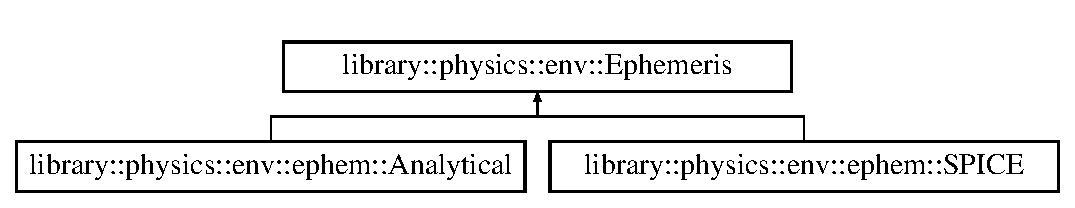
\includegraphics[height=2.000000cm]{classlibrary_1_1physics_1_1env_1_1_ephemeris}
\end{center}
\end{figure}
\subsection*{Public Member Functions}
\begin{DoxyCompactItemize}
\item 
\hyperlink{classlibrary_1_1physics_1_1env_1_1_ephemeris_a99282f212b17cc6a4eb63f99e6b16f69}{Ephemeris} ()
\item 
virtual \hyperlink{classlibrary_1_1physics_1_1env_1_1_ephemeris_af2459c2cc219c926f18e540fd0ebbaac}{$\sim$\+Ephemeris} ()=0
\item 
virtual \hyperlink{classlibrary_1_1physics_1_1env_1_1_ephemeris}{Ephemeris} $\ast$ \hyperlink{classlibrary_1_1physics_1_1env_1_1_ephemeris_a7ddecd88d91f79ff204100eb9607b591}{clone} () const =0
\item 
virtual bool \hyperlink{classlibrary_1_1physics_1_1env_1_1_ephemeris_abf61a03e24dd146199381db14d1d7c68}{is\+Defined} () const =0
\item 
virtual Shared$<$ const \hyperlink{classlibrary_1_1physics_1_1coord_1_1_frame}{Frame} $>$ \hyperlink{classlibrary_1_1physics_1_1env_1_1_ephemeris_ac832f493239ace4d53c1c5130c1dad31}{access\+Frame} () const =0
\end{DoxyCompactItemize}


\subsection{Detailed Description}
https\+://en.wikipedia.\+org/wiki/\+Fundamental\+\_\+ephemeris 

\subsection{Constructor \& Destructor Documentation}
\mbox{\Hypertarget{classlibrary_1_1physics_1_1env_1_1_ephemeris_a99282f212b17cc6a4eb63f99e6b16f69}\label{classlibrary_1_1physics_1_1env_1_1_ephemeris_a99282f212b17cc6a4eb63f99e6b16f69}} 
\index{library\+::physics\+::env\+::\+Ephemeris@{library\+::physics\+::env\+::\+Ephemeris}!Ephemeris@{Ephemeris}}
\index{Ephemeris@{Ephemeris}!library\+::physics\+::env\+::\+Ephemeris@{library\+::physics\+::env\+::\+Ephemeris}}
\subsubsection{\texorpdfstring{Ephemeris()}{Ephemeris()}}
{\footnotesize\ttfamily library\+::physics\+::env\+::\+Ephemeris\+::\+Ephemeris (\begin{DoxyParamCaption}{ }\end{DoxyParamCaption})}

\mbox{\Hypertarget{classlibrary_1_1physics_1_1env_1_1_ephemeris_af2459c2cc219c926f18e540fd0ebbaac}\label{classlibrary_1_1physics_1_1env_1_1_ephemeris_af2459c2cc219c926f18e540fd0ebbaac}} 
\index{library\+::physics\+::env\+::\+Ephemeris@{library\+::physics\+::env\+::\+Ephemeris}!````~Ephemeris@{$\sim$\+Ephemeris}}
\index{````~Ephemeris@{$\sim$\+Ephemeris}!library\+::physics\+::env\+::\+Ephemeris@{library\+::physics\+::env\+::\+Ephemeris}}
\subsubsection{\texorpdfstring{$\sim$\+Ephemeris()}{~Ephemeris()}}
{\footnotesize\ttfamily library\+::physics\+::env\+::\+Ephemeris\+::$\sim$\+Ephemeris (\begin{DoxyParamCaption}{ }\end{DoxyParamCaption})\hspace{0.3cm}{\ttfamily [pure virtual]}}



\subsection{Member Function Documentation}
\mbox{\Hypertarget{classlibrary_1_1physics_1_1env_1_1_ephemeris_ac832f493239ace4d53c1c5130c1dad31}\label{classlibrary_1_1physics_1_1env_1_1_ephemeris_ac832f493239ace4d53c1c5130c1dad31}} 
\index{library\+::physics\+::env\+::\+Ephemeris@{library\+::physics\+::env\+::\+Ephemeris}!access\+Frame@{access\+Frame}}
\index{access\+Frame@{access\+Frame}!library\+::physics\+::env\+::\+Ephemeris@{library\+::physics\+::env\+::\+Ephemeris}}
\subsubsection{\texorpdfstring{access\+Frame()}{accessFrame()}}
{\footnotesize\ttfamily virtual Shared$<$const \hyperlink{classlibrary_1_1physics_1_1coord_1_1_frame}{Frame}$>$ library\+::physics\+::env\+::\+Ephemeris\+::access\+Frame (\begin{DoxyParamCaption}{ }\end{DoxyParamCaption}) const\hspace{0.3cm}{\ttfamily [pure virtual]}}



Implemented in \hyperlink{classlibrary_1_1physics_1_1env_1_1ephem_1_1_s_p_i_c_e_a20b94d4f05b17a2eb3ba986464da44a8}{library\+::physics\+::env\+::ephem\+::\+S\+P\+I\+CE}, and \hyperlink{classlibrary_1_1physics_1_1env_1_1ephem_1_1_analytical_ad16f575a7804bd29710030289d5630b1}{library\+::physics\+::env\+::ephem\+::\+Analytical}.

\mbox{\Hypertarget{classlibrary_1_1physics_1_1env_1_1_ephemeris_a7ddecd88d91f79ff204100eb9607b591}\label{classlibrary_1_1physics_1_1env_1_1_ephemeris_a7ddecd88d91f79ff204100eb9607b591}} 
\index{library\+::physics\+::env\+::\+Ephemeris@{library\+::physics\+::env\+::\+Ephemeris}!clone@{clone}}
\index{clone@{clone}!library\+::physics\+::env\+::\+Ephemeris@{library\+::physics\+::env\+::\+Ephemeris}}
\subsubsection{\texorpdfstring{clone()}{clone()}}
{\footnotesize\ttfamily virtual \hyperlink{classlibrary_1_1physics_1_1env_1_1_ephemeris}{Ephemeris}$\ast$ library\+::physics\+::env\+::\+Ephemeris\+::clone (\begin{DoxyParamCaption}{ }\end{DoxyParamCaption}) const\hspace{0.3cm}{\ttfamily [pure virtual]}}



Implemented in \hyperlink{classlibrary_1_1physics_1_1env_1_1ephem_1_1_s_p_i_c_e_a7d397f5472ec2e14d85fa493cb7c9ae0}{library\+::physics\+::env\+::ephem\+::\+S\+P\+I\+CE}, and \hyperlink{classlibrary_1_1physics_1_1env_1_1ephem_1_1_analytical_acd51ca99177b1433b6623829ae003bec}{library\+::physics\+::env\+::ephem\+::\+Analytical}.

\mbox{\Hypertarget{classlibrary_1_1physics_1_1env_1_1_ephemeris_abf61a03e24dd146199381db14d1d7c68}\label{classlibrary_1_1physics_1_1env_1_1_ephemeris_abf61a03e24dd146199381db14d1d7c68}} 
\index{library\+::physics\+::env\+::\+Ephemeris@{library\+::physics\+::env\+::\+Ephemeris}!is\+Defined@{is\+Defined}}
\index{is\+Defined@{is\+Defined}!library\+::physics\+::env\+::\+Ephemeris@{library\+::physics\+::env\+::\+Ephemeris}}
\subsubsection{\texorpdfstring{is\+Defined()}{isDefined()}}
{\footnotesize\ttfamily virtual bool library\+::physics\+::env\+::\+Ephemeris\+::is\+Defined (\begin{DoxyParamCaption}{ }\end{DoxyParamCaption}) const\hspace{0.3cm}{\ttfamily [pure virtual]}}



Implemented in \hyperlink{classlibrary_1_1physics_1_1env_1_1ephem_1_1_s_p_i_c_e_a54fb3fb8768a72f515231dac083eb9cb}{library\+::physics\+::env\+::ephem\+::\+S\+P\+I\+CE}, and \hyperlink{classlibrary_1_1physics_1_1env_1_1ephem_1_1_analytical_a0c0fe5d8326ba439bb0b51e7536ab0fd}{library\+::physics\+::env\+::ephem\+::\+Analytical}.



The documentation for this class was generated from the following files\+:\begin{DoxyCompactItemize}
\item 
include/\+Library/\+Physics/\+Environment/\hyperlink{_ephemeris_8hpp}{Ephemeris.\+hpp}\item 
src/\+Library/\+Physics/\+Environment/\hyperlink{_ephemeris_8cpp}{Ephemeris.\+cpp}\end{DoxyCompactItemize}

\hypertarget{classlibrary_1_1physics_1_1coord_1_1frame_1_1provider_1_1iers_1_1_finals2000_a}{}\section{library\+:\+:physics\+:\+:coord\+:\+:frame\+:\+:provider\+:\+:iers\+:\+:Finals2000A Class Reference}
\label{classlibrary_1_1physics_1_1coord_1_1frame_1_1provider_1_1iers_1_1_finals2000_a}\index{library\+::physics\+::coord\+::frame\+::provider\+::iers\+::\+Finals2000A@{library\+::physics\+::coord\+::frame\+::provider\+::iers\+::\+Finals2000A}}


Standard Rapid E\+OP \hyperlink{structlibrary_1_1physics_1_1coord_1_1frame_1_1provider_1_1iers_1_1_finals2000_a_1_1_data}{Data} since 01. January 1992 (I\+A\+U2000)  




{\ttfamily \#include $<$Finals2000\+A.\+hpp$>$}

\subsection*{Classes}
\begin{DoxyCompactItemize}
\item 
struct \hyperlink{structlibrary_1_1physics_1_1coord_1_1frame_1_1provider_1_1iers_1_1_finals2000_a_1_1_data}{Data}
\end{DoxyCompactItemize}
\subsection*{Public Member Functions}
\begin{DoxyCompactItemize}
\item 
bool \hyperlink{classlibrary_1_1physics_1_1coord_1_1frame_1_1provider_1_1iers_1_1_finals2000_a_af87374c2ad6f1f81aad5abfe1b3b90f9}{is\+Defined} () const
\item 
\hyperlink{classlibrary_1_1physics_1_1time_1_1_interval}{Interval} \hyperlink{classlibrary_1_1physics_1_1coord_1_1frame_1_1provider_1_1iers_1_1_finals2000_a_a327ff24883eb53123cc24138e9269c48}{get\+Interval} () const
\item 
Vector2d \hyperlink{classlibrary_1_1physics_1_1coord_1_1frame_1_1provider_1_1iers_1_1_finals2000_a_a9bb453db22a0196f015f346c986d89dd}{get\+Polar\+Motion\+At} (const \hyperlink{classlibrary_1_1physics_1_1time_1_1_instant}{Instant} \&an\+Instant) const
\item 
Real \hyperlink{classlibrary_1_1physics_1_1coord_1_1frame_1_1provider_1_1iers_1_1_finals2000_a_aa76c7ba7198ef2bd5f9b9feb8adb5ee8}{get\+Ut1\+Minus\+Utc\+At} (const \hyperlink{classlibrary_1_1physics_1_1time_1_1_instant}{Instant} \&an\+Instant) const
\item 
Real \hyperlink{classlibrary_1_1physics_1_1coord_1_1frame_1_1provider_1_1iers_1_1_finals2000_a_a8ea6986b80b0777ec7b11a9a0ee60d70}{get\+Lod\+At} (const \hyperlink{classlibrary_1_1physics_1_1time_1_1_instant}{Instant} \&an\+Instant) const
\item 
\hyperlink{structlibrary_1_1physics_1_1coord_1_1frame_1_1provider_1_1iers_1_1_finals2000_a_1_1_data}{Finals2000\+A\+::\+Data} \hyperlink{classlibrary_1_1physics_1_1coord_1_1frame_1_1provider_1_1iers_1_1_finals2000_a_a5e7b1a165152fd3ccf0bbfdc859dd3f5}{get\+Data\+At} (const \hyperlink{classlibrary_1_1physics_1_1time_1_1_instant}{Instant} \&an\+Instant) const
\end{DoxyCompactItemize}
\subsection*{Static Public Member Functions}
\begin{DoxyCompactItemize}
\item 
static \hyperlink{classlibrary_1_1physics_1_1coord_1_1frame_1_1provider_1_1iers_1_1_finals2000_a}{Finals2000A} \hyperlink{classlibrary_1_1physics_1_1coord_1_1frame_1_1provider_1_1iers_1_1_finals2000_a_ab860c78d5315d96fdd2e53e5f6a3efd1}{Undefined} ()
\item 
static \hyperlink{classlibrary_1_1physics_1_1coord_1_1frame_1_1provider_1_1iers_1_1_finals2000_a}{Finals2000A} \hyperlink{classlibrary_1_1physics_1_1coord_1_1frame_1_1provider_1_1iers_1_1_finals2000_a_a280812cd766e12620b7dc15254c92779}{Load} (const fs\+::\+File \&a\+File)
\end{DoxyCompactItemize}
\subsection*{Friends}
\begin{DoxyCompactItemize}
\item 
std\+::ostream \& \hyperlink{classlibrary_1_1physics_1_1coord_1_1frame_1_1provider_1_1iers_1_1_finals2000_a_ade92763eb1cb719a4a499af1beb72b43}{operator$<$$<$} (std\+::ostream \&an\+Output\+Stream, const \hyperlink{classlibrary_1_1physics_1_1coord_1_1frame_1_1provider_1_1iers_1_1_finals2000_a}{Finals2000A} \&a\+Finals2000A)
\end{DoxyCompactItemize}


\subsection{Detailed Description}
Standard Rapid E\+OP \hyperlink{structlibrary_1_1physics_1_1coord_1_1frame_1_1provider_1_1iers_1_1_finals2000_a_1_1_data}{Data} since 01. January 1992 (I\+A\+U2000) 

This file (updated weekly) is the complete Earth orientation data set, since 1 January 1992 with 1 year of predictions. The nutation series in dX and dY uses the I\+AU 2000A Nutation Theory.

http\+://maia.usno.\+navy.\+mil/ser7/readme.finals2000A https\+://datacenter.iers.\+org/eop/-\//somos/5\+Rgv/latest/10 

\subsection{Member Function Documentation}
\mbox{\Hypertarget{classlibrary_1_1physics_1_1coord_1_1frame_1_1provider_1_1iers_1_1_finals2000_a_a5e7b1a165152fd3ccf0bbfdc859dd3f5}\label{classlibrary_1_1physics_1_1coord_1_1frame_1_1provider_1_1iers_1_1_finals2000_a_a5e7b1a165152fd3ccf0bbfdc859dd3f5}} 
\index{library\+::physics\+::coord\+::frame\+::provider\+::iers\+::\+Finals2000A@{library\+::physics\+::coord\+::frame\+::provider\+::iers\+::\+Finals2000A}!get\+Data\+At@{get\+Data\+At}}
\index{get\+Data\+At@{get\+Data\+At}!library\+::physics\+::coord\+::frame\+::provider\+::iers\+::\+Finals2000A@{library\+::physics\+::coord\+::frame\+::provider\+::iers\+::\+Finals2000A}}
\subsubsection{\texorpdfstring{get\+Data\+At()}{getDataAt()}}
{\footnotesize\ttfamily \hyperlink{structlibrary_1_1physics_1_1coord_1_1frame_1_1provider_1_1iers_1_1_finals2000_a_1_1_data}{Finals2000\+A\+::\+Data} library\+::physics\+::coord\+::frame\+::provider\+::iers\+::\+Finals2000\+A\+::get\+Data\+At (\begin{DoxyParamCaption}\item[{const \hyperlink{classlibrary_1_1physics_1_1time_1_1_instant}{Instant} \&}]{an\+Instant }\end{DoxyParamCaption}) const}

\mbox{\Hypertarget{classlibrary_1_1physics_1_1coord_1_1frame_1_1provider_1_1iers_1_1_finals2000_a_a327ff24883eb53123cc24138e9269c48}\label{classlibrary_1_1physics_1_1coord_1_1frame_1_1provider_1_1iers_1_1_finals2000_a_a327ff24883eb53123cc24138e9269c48}} 
\index{library\+::physics\+::coord\+::frame\+::provider\+::iers\+::\+Finals2000A@{library\+::physics\+::coord\+::frame\+::provider\+::iers\+::\+Finals2000A}!get\+Interval@{get\+Interval}}
\index{get\+Interval@{get\+Interval}!library\+::physics\+::coord\+::frame\+::provider\+::iers\+::\+Finals2000A@{library\+::physics\+::coord\+::frame\+::provider\+::iers\+::\+Finals2000A}}
\subsubsection{\texorpdfstring{get\+Interval()}{getInterval()}}
{\footnotesize\ttfamily \hyperlink{classlibrary_1_1physics_1_1time_1_1_interval}{Interval} library\+::physics\+::coord\+::frame\+::provider\+::iers\+::\+Finals2000\+A\+::get\+Interval (\begin{DoxyParamCaption}{ }\end{DoxyParamCaption}) const}

\mbox{\Hypertarget{classlibrary_1_1physics_1_1coord_1_1frame_1_1provider_1_1iers_1_1_finals2000_a_a8ea6986b80b0777ec7b11a9a0ee60d70}\label{classlibrary_1_1physics_1_1coord_1_1frame_1_1provider_1_1iers_1_1_finals2000_a_a8ea6986b80b0777ec7b11a9a0ee60d70}} 
\index{library\+::physics\+::coord\+::frame\+::provider\+::iers\+::\+Finals2000A@{library\+::physics\+::coord\+::frame\+::provider\+::iers\+::\+Finals2000A}!get\+Lod\+At@{get\+Lod\+At}}
\index{get\+Lod\+At@{get\+Lod\+At}!library\+::physics\+::coord\+::frame\+::provider\+::iers\+::\+Finals2000A@{library\+::physics\+::coord\+::frame\+::provider\+::iers\+::\+Finals2000A}}
\subsubsection{\texorpdfstring{get\+Lod\+At()}{getLodAt()}}
{\footnotesize\ttfamily Real library\+::physics\+::coord\+::frame\+::provider\+::iers\+::\+Finals2000\+A\+::get\+Lod\+At (\begin{DoxyParamCaption}\item[{const \hyperlink{classlibrary_1_1physics_1_1time_1_1_instant}{Instant} \&}]{an\+Instant }\end{DoxyParamCaption}) const}

\mbox{\Hypertarget{classlibrary_1_1physics_1_1coord_1_1frame_1_1provider_1_1iers_1_1_finals2000_a_a9bb453db22a0196f015f346c986d89dd}\label{classlibrary_1_1physics_1_1coord_1_1frame_1_1provider_1_1iers_1_1_finals2000_a_a9bb453db22a0196f015f346c986d89dd}} 
\index{library\+::physics\+::coord\+::frame\+::provider\+::iers\+::\+Finals2000A@{library\+::physics\+::coord\+::frame\+::provider\+::iers\+::\+Finals2000A}!get\+Polar\+Motion\+At@{get\+Polar\+Motion\+At}}
\index{get\+Polar\+Motion\+At@{get\+Polar\+Motion\+At}!library\+::physics\+::coord\+::frame\+::provider\+::iers\+::\+Finals2000A@{library\+::physics\+::coord\+::frame\+::provider\+::iers\+::\+Finals2000A}}
\subsubsection{\texorpdfstring{get\+Polar\+Motion\+At()}{getPolarMotionAt()}}
{\footnotesize\ttfamily Vector2d library\+::physics\+::coord\+::frame\+::provider\+::iers\+::\+Finals2000\+A\+::get\+Polar\+Motion\+At (\begin{DoxyParamCaption}\item[{const \hyperlink{classlibrary_1_1physics_1_1time_1_1_instant}{Instant} \&}]{an\+Instant }\end{DoxyParamCaption}) const}

\mbox{\Hypertarget{classlibrary_1_1physics_1_1coord_1_1frame_1_1provider_1_1iers_1_1_finals2000_a_aa76c7ba7198ef2bd5f9b9feb8adb5ee8}\label{classlibrary_1_1physics_1_1coord_1_1frame_1_1provider_1_1iers_1_1_finals2000_a_aa76c7ba7198ef2bd5f9b9feb8adb5ee8}} 
\index{library\+::physics\+::coord\+::frame\+::provider\+::iers\+::\+Finals2000A@{library\+::physics\+::coord\+::frame\+::provider\+::iers\+::\+Finals2000A}!get\+Ut1\+Minus\+Utc\+At@{get\+Ut1\+Minus\+Utc\+At}}
\index{get\+Ut1\+Minus\+Utc\+At@{get\+Ut1\+Minus\+Utc\+At}!library\+::physics\+::coord\+::frame\+::provider\+::iers\+::\+Finals2000A@{library\+::physics\+::coord\+::frame\+::provider\+::iers\+::\+Finals2000A}}
\subsubsection{\texorpdfstring{get\+Ut1\+Minus\+Utc\+At()}{getUt1MinusUtcAt()}}
{\footnotesize\ttfamily Real library\+::physics\+::coord\+::frame\+::provider\+::iers\+::\+Finals2000\+A\+::get\+Ut1\+Minus\+Utc\+At (\begin{DoxyParamCaption}\item[{const \hyperlink{classlibrary_1_1physics_1_1time_1_1_instant}{Instant} \&}]{an\+Instant }\end{DoxyParamCaption}) const}

\mbox{\Hypertarget{classlibrary_1_1physics_1_1coord_1_1frame_1_1provider_1_1iers_1_1_finals2000_a_af87374c2ad6f1f81aad5abfe1b3b90f9}\label{classlibrary_1_1physics_1_1coord_1_1frame_1_1provider_1_1iers_1_1_finals2000_a_af87374c2ad6f1f81aad5abfe1b3b90f9}} 
\index{library\+::physics\+::coord\+::frame\+::provider\+::iers\+::\+Finals2000A@{library\+::physics\+::coord\+::frame\+::provider\+::iers\+::\+Finals2000A}!is\+Defined@{is\+Defined}}
\index{is\+Defined@{is\+Defined}!library\+::physics\+::coord\+::frame\+::provider\+::iers\+::\+Finals2000A@{library\+::physics\+::coord\+::frame\+::provider\+::iers\+::\+Finals2000A}}
\subsubsection{\texorpdfstring{is\+Defined()}{isDefined()}}
{\footnotesize\ttfamily bool library\+::physics\+::coord\+::frame\+::provider\+::iers\+::\+Finals2000\+A\+::is\+Defined (\begin{DoxyParamCaption}{ }\end{DoxyParamCaption}) const}

\mbox{\Hypertarget{classlibrary_1_1physics_1_1coord_1_1frame_1_1provider_1_1iers_1_1_finals2000_a_a280812cd766e12620b7dc15254c92779}\label{classlibrary_1_1physics_1_1coord_1_1frame_1_1provider_1_1iers_1_1_finals2000_a_a280812cd766e12620b7dc15254c92779}} 
\index{library\+::physics\+::coord\+::frame\+::provider\+::iers\+::\+Finals2000A@{library\+::physics\+::coord\+::frame\+::provider\+::iers\+::\+Finals2000A}!Load@{Load}}
\index{Load@{Load}!library\+::physics\+::coord\+::frame\+::provider\+::iers\+::\+Finals2000A@{library\+::physics\+::coord\+::frame\+::provider\+::iers\+::\+Finals2000A}}
\subsubsection{\texorpdfstring{Load()}{Load()}}
{\footnotesize\ttfamily \hyperlink{classlibrary_1_1physics_1_1coord_1_1frame_1_1provider_1_1iers_1_1_finals2000_a}{Finals2000A} library\+::physics\+::coord\+::frame\+::provider\+::iers\+::\+Finals2000\+A\+::\+Load (\begin{DoxyParamCaption}\item[{const fs\+::\+File \&}]{a\+File }\end{DoxyParamCaption})\hspace{0.3cm}{\ttfamily [static]}}

\mbox{\Hypertarget{classlibrary_1_1physics_1_1coord_1_1frame_1_1provider_1_1iers_1_1_finals2000_a_ab860c78d5315d96fdd2e53e5f6a3efd1}\label{classlibrary_1_1physics_1_1coord_1_1frame_1_1provider_1_1iers_1_1_finals2000_a_ab860c78d5315d96fdd2e53e5f6a3efd1}} 
\index{library\+::physics\+::coord\+::frame\+::provider\+::iers\+::\+Finals2000A@{library\+::physics\+::coord\+::frame\+::provider\+::iers\+::\+Finals2000A}!Undefined@{Undefined}}
\index{Undefined@{Undefined}!library\+::physics\+::coord\+::frame\+::provider\+::iers\+::\+Finals2000A@{library\+::physics\+::coord\+::frame\+::provider\+::iers\+::\+Finals2000A}}
\subsubsection{\texorpdfstring{Undefined()}{Undefined()}}
{\footnotesize\ttfamily \hyperlink{classlibrary_1_1physics_1_1coord_1_1frame_1_1provider_1_1iers_1_1_finals2000_a}{Finals2000A} library\+::physics\+::coord\+::frame\+::provider\+::iers\+::\+Finals2000\+A\+::\+Undefined (\begin{DoxyParamCaption}{ }\end{DoxyParamCaption})\hspace{0.3cm}{\ttfamily [static]}}



\subsection{Friends And Related Function Documentation}
\mbox{\Hypertarget{classlibrary_1_1physics_1_1coord_1_1frame_1_1provider_1_1iers_1_1_finals2000_a_ade92763eb1cb719a4a499af1beb72b43}\label{classlibrary_1_1physics_1_1coord_1_1frame_1_1provider_1_1iers_1_1_finals2000_a_ade92763eb1cb719a4a499af1beb72b43}} 
\index{library\+::physics\+::coord\+::frame\+::provider\+::iers\+::\+Finals2000A@{library\+::physics\+::coord\+::frame\+::provider\+::iers\+::\+Finals2000A}!operator$<$$<$@{operator$<$$<$}}
\index{operator$<$$<$@{operator$<$$<$}!library\+::physics\+::coord\+::frame\+::provider\+::iers\+::\+Finals2000A@{library\+::physics\+::coord\+::frame\+::provider\+::iers\+::\+Finals2000A}}
\subsubsection{\texorpdfstring{operator$<$$<$}{operator<<}}
{\footnotesize\ttfamily std\+::ostream\& operator$<$$<$ (\begin{DoxyParamCaption}\item[{std\+::ostream \&}]{an\+Output\+Stream,  }\item[{const \hyperlink{classlibrary_1_1physics_1_1coord_1_1frame_1_1provider_1_1iers_1_1_finals2000_a}{Finals2000A} \&}]{a\+Finals2000A }\end{DoxyParamCaption})\hspace{0.3cm}{\ttfamily [friend]}}



The documentation for this class was generated from the following files\+:\begin{DoxyCompactItemize}
\item 
include/\+Library/\+Physics/\+Coordinate/\+Frame/\+Providers/\+I\+E\+R\+S/\hyperlink{_finals2000_a_8hpp}{Finals2000\+A.\+hpp}\item 
src/\+Library/\+Physics/\+Coordinate/\+Frame/\+Providers/\+I\+E\+R\+S/\hyperlink{_finals2000_a_8cpp}{Finals2000\+A.\+cpp}\end{DoxyCompactItemize}

\hypertarget{classlibrary_1_1physics_1_1coord_1_1_frame}{}\section{library\+:\+:physics\+:\+:coord\+:\+:Frame Class Reference}
\label{classlibrary_1_1physics_1_1coord_1_1_frame}\index{library\+::physics\+::coord\+::\+Frame@{library\+::physics\+::coord\+::\+Frame}}


Reference frame.  




{\ttfamily \#include $<$Frame.\+hpp$>$}

Inheritance diagram for library\+:\+:physics\+:\+:coord\+:\+:Frame\+:\begin{figure}[H]
\begin{center}
\leavevmode
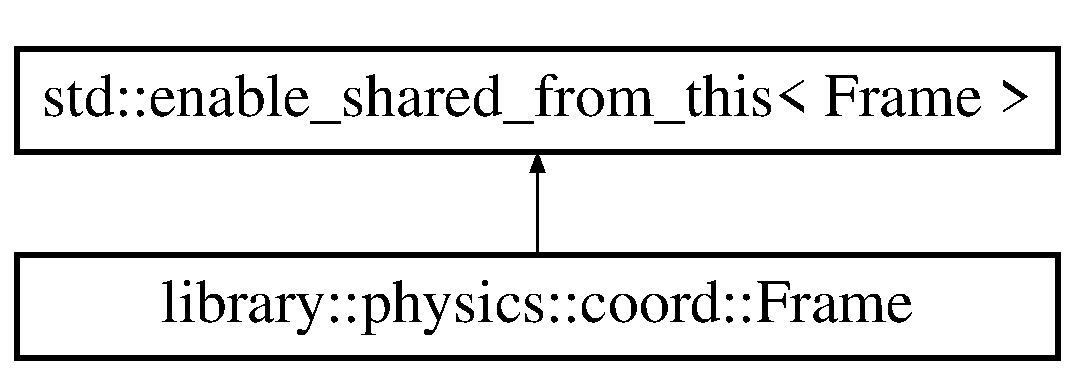
\includegraphics[height=2.000000cm]{classlibrary_1_1physics_1_1coord_1_1_frame}
\end{center}
\end{figure}
\subsection*{Public Member Functions}
\begin{DoxyCompactItemize}
\item 
\hyperlink{classlibrary_1_1physics_1_1coord_1_1_frame_a7a4b031eff12e290c0ccacb7d5a47dfd}{$\sim$\+Frame} ()
\begin{DoxyCompactList}\small\item\em Destructor. \end{DoxyCompactList}\item 
bool \hyperlink{classlibrary_1_1physics_1_1coord_1_1_frame_a19c5c4ce3b1669a774980d9c3f18fe6c}{operator==} (const \hyperlink{classlibrary_1_1physics_1_1coord_1_1_frame}{Frame} \&a\+Frame) const
\item 
bool \hyperlink{classlibrary_1_1physics_1_1coord_1_1_frame_a2b3b046c3779b4281f14601302446169}{operator!=} (const \hyperlink{classlibrary_1_1physics_1_1coord_1_1_frame}{Frame} \&a\+Frame) const
\item 
bool \hyperlink{classlibrary_1_1physics_1_1coord_1_1_frame_ad5a450dd6740fc5a27473e661375dde6}{is\+Defined} () const
\item 
bool \hyperlink{classlibrary_1_1physics_1_1coord_1_1_frame_a894d1ac6152e28dbb749058ca6ffd663}{is\+Quasi\+Inertial} () const
\item 
bool \hyperlink{classlibrary_1_1physics_1_1coord_1_1_frame_afd83dec4bf4e2aabc2b31019b282965e}{has\+Parent} () const
\item 
Shared$<$ const \hyperlink{classlibrary_1_1physics_1_1coord_1_1_frame}{Frame} $>$ \hyperlink{classlibrary_1_1physics_1_1coord_1_1_frame_a30d789571e08b1fbcddbdde656a95a79}{access\+Parent} () const
\item 
Shared$<$ const \hyperlink{classlibrary_1_1physics_1_1coord_1_1_frame}{Frame} $>$ \hyperlink{classlibrary_1_1physics_1_1coord_1_1_frame_abcadc7427a971aa37a66123cb9b8322b}{access\+Ancestor} (const Uint8 an\+Ancestor\+Degree) const
\item 
Shared$<$ const \hyperlink{classlibrary_1_1physics_1_1coord_1_1frame_1_1_provider}{Provider} $>$ \hyperlink{classlibrary_1_1physics_1_1coord_1_1_frame_a5da9096ace352a91d272677cc159c059}{access\+Provider} () const
\item 
String \hyperlink{classlibrary_1_1physics_1_1coord_1_1_frame_afec582db83d2bf93b2b070f8557ee760}{get\+Name} () const
\item 
\hyperlink{classlibrary_1_1physics_1_1coord_1_1_position}{Position} \hyperlink{classlibrary_1_1physics_1_1coord_1_1_frame_aa68223b40939d6dd45ace7746805d33c}{get\+Origin\+In} (const Shared$<$ const \hyperlink{classlibrary_1_1physics_1_1coord_1_1_frame}{Frame} $>$ \&a\+Frame, const \hyperlink{classlibrary_1_1physics_1_1time_1_1_instant}{Instant} \&an\+Instant) const
\item 
\hyperlink{classlibrary_1_1physics_1_1coord_1_1_velocity}{Velocity} \hyperlink{classlibrary_1_1physics_1_1coord_1_1_frame_ae7974e759c97f32ccc966cbcc3baf77c}{get\+Velocity\+In} (const Shared$<$ const \hyperlink{classlibrary_1_1physics_1_1coord_1_1_frame}{Frame} $>$ \&a\+Frame, const \hyperlink{classlibrary_1_1physics_1_1time_1_1_instant}{Instant} \&an\+Instant) const
\item 
\hyperlink{classlibrary_1_1physics_1_1coord_1_1_axes}{Axes} \hyperlink{classlibrary_1_1physics_1_1coord_1_1_frame_abd6fc9109e37433d4b223cfb291edb20}{get\+Axes\+In} (const Shared$<$ const \hyperlink{classlibrary_1_1physics_1_1coord_1_1_frame}{Frame} $>$ \&a\+Frame, const \hyperlink{classlibrary_1_1physics_1_1time_1_1_instant}{Instant} \&an\+Instant) const
\item 
\hyperlink{classlibrary_1_1physics_1_1coord_1_1_transform}{Transform} \hyperlink{classlibrary_1_1physics_1_1coord_1_1_frame_a567715e72b885f8c7ec0ab7a3d068240}{get\+Transform\+To} (const Shared$<$ const \hyperlink{classlibrary_1_1physics_1_1coord_1_1_frame}{Frame} $>$ \&a\+Frame, const \hyperlink{classlibrary_1_1physics_1_1time_1_1_instant}{Instant} \&an\+Instant) const
\end{DoxyCompactItemize}
\subsection*{Static Public Member Functions}
\begin{DoxyCompactItemize}
\item 
static Shared$<$ const \hyperlink{classlibrary_1_1physics_1_1coord_1_1_frame}{Frame} $>$ \hyperlink{classlibrary_1_1physics_1_1coord_1_1_frame_aed834a54cd63338b3d9cc4bee2989d9d}{Undefined} ()
\item 
static Shared$<$ const \hyperlink{classlibrary_1_1physics_1_1coord_1_1_frame}{Frame} $>$ \hyperlink{classlibrary_1_1physics_1_1coord_1_1_frame_a7c325ecdb25f617babb9bfcf2d0f56e5}{I\+C\+RF} ()
\item 
static Shared$<$ const \hyperlink{classlibrary_1_1physics_1_1coord_1_1_frame}{Frame} $>$ \hyperlink{classlibrary_1_1physics_1_1coord_1_1_frame_af69afe3a03044d0c8245fd814dc2e3ce}{G\+C\+RF} ()
\item 
static Shared$<$ const \hyperlink{classlibrary_1_1physics_1_1coord_1_1_frame}{Frame} $>$ \hyperlink{classlibrary_1_1physics_1_1coord_1_1_frame_a16840fb31ca3fdaff3465a714b486683}{E\+M\+E2000} ()
\item 
static Shared$<$ const \hyperlink{classlibrary_1_1physics_1_1coord_1_1_frame}{Frame} $>$ \hyperlink{classlibrary_1_1physics_1_1coord_1_1_frame_a1c59f635fe7a36f416994c83533bfb40}{T\+E\+ME} ()
\item 
static Shared$<$ const \hyperlink{classlibrary_1_1physics_1_1coord_1_1_frame}{Frame} $>$ \hyperlink{classlibrary_1_1physics_1_1coord_1_1_frame_acadb0a99f334abe26797fd846e1ca22e}{T\+E\+M\+E\+Of\+Epoch} (const \hyperlink{classlibrary_1_1physics_1_1time_1_1_instant}{Instant} \&an\+Epoch)
\item 
static Shared$<$ const \hyperlink{classlibrary_1_1physics_1_1coord_1_1_frame}{Frame} $>$ \hyperlink{classlibrary_1_1physics_1_1coord_1_1_frame_a0786e3028527a43e423936989a9cd294}{C\+I\+RF} ()
\item 
static Shared$<$ const \hyperlink{classlibrary_1_1physics_1_1coord_1_1_frame}{Frame} $>$ \hyperlink{classlibrary_1_1physics_1_1coord_1_1_frame_af03b39a76e957c83375cb3439f3d6a5a}{T\+I\+RF} ()
\item 
static Shared$<$ const \hyperlink{classlibrary_1_1physics_1_1coord_1_1_frame}{Frame} $>$ \hyperlink{classlibrary_1_1physics_1_1coord_1_1_frame_aae0930a623efe205c837b167981eec4d}{I\+T\+RF} ()
\item 
static Shared$<$ const \hyperlink{classlibrary_1_1physics_1_1coord_1_1_frame}{Frame} $>$ \hyperlink{classlibrary_1_1physics_1_1coord_1_1_frame_ad4b2b9a19b234d27ea56ea8b21107f9b}{With\+Name} (const String \&a\+Name)
\item 
static Shared$<$ const \hyperlink{classlibrary_1_1physics_1_1coord_1_1_frame}{Frame} $>$ \hyperlink{classlibrary_1_1physics_1_1coord_1_1_frame_acdadad4d650b63c1d4ad05d5268e0b79}{Construct} (const String \&a\+Name, bool \hyperlink{classlibrary_1_1physics_1_1coord_1_1_frame_a894d1ac6152e28dbb749058ca6ffd663}{is\+Quasi\+Inertial}, const Shared$<$ const \hyperlink{classlibrary_1_1physics_1_1coord_1_1_frame}{Frame} $>$ \&a\+Parent\+Frame, const Shared$<$ const \hyperlink{classlibrary_1_1physics_1_1coord_1_1frame_1_1_provider}{Provider} $>$ \&a\+Provider)
\begin{DoxyCompactList}\small\item\em Constructor. \end{DoxyCompactList}\item 
static void \hyperlink{classlibrary_1_1physics_1_1coord_1_1_frame_a2d4229290a0332c70240ebc8b02bd132}{Destruct} (const String \&a\+Name)
\end{DoxyCompactItemize}
\subsection*{Protected Member Functions}
\begin{DoxyCompactItemize}
\item 
\hyperlink{classlibrary_1_1physics_1_1coord_1_1_frame_a6a8410c8b29584fe2c2c78370c72f695}{Frame} (const String \&a\+Name, bool \hyperlink{classlibrary_1_1physics_1_1coord_1_1_frame_a894d1ac6152e28dbb749058ca6ffd663}{is\+Quasi\+Inertial}, const Shared$<$ const \hyperlink{classlibrary_1_1physics_1_1coord_1_1_frame}{Frame} $>$ \&a\+Parent\+Frame, const Shared$<$ const \hyperlink{classlibrary_1_1physics_1_1coord_1_1frame_1_1_provider}{Provider} $>$ \&a\+Provider)
\item 
\hyperlink{classlibrary_1_1physics_1_1coord_1_1_frame_abacc320c21194a591bf76612d91bafb9}{Frame} (const \hyperlink{classlibrary_1_1physics_1_1coord_1_1_frame}{Frame} \&a\+Frame)=default
\item 
\hyperlink{classlibrary_1_1physics_1_1coord_1_1_frame}{Frame} \& \hyperlink{classlibrary_1_1physics_1_1coord_1_1_frame_a31c2c947b4b27a9873d4eda7816e8247}{operator=} (const \hyperlink{classlibrary_1_1physics_1_1coord_1_1_frame}{Frame} \&a\+Frame)=default
\end{DoxyCompactItemize}
\subsection*{Friends}
\begin{DoxyCompactItemize}
\item 
std\+::ostream \& \hyperlink{classlibrary_1_1physics_1_1coord_1_1_frame_a509ac1926cfc3553748bace204e2b1cc}{operator$<$$<$} (std\+::ostream \&an\+Output\+Stream, const \hyperlink{classlibrary_1_1physics_1_1coord_1_1_frame}{Frame} \&a\+Frame)
\end{DoxyCompactItemize}


\subsection{Detailed Description}
Reference frame. 

https\+://en.wikipedia.\+org/wiki/\+Frame\+\_\+of\+\_\+reference \begin{DoxyNote}{Note}
Implementation heavily inspired by (the great!) \href{https://www.orekit.org/static/architecture/frames.html}{\tt https\+://www.\+orekit.\+org/static/architecture/frames.\+html} 
\end{DoxyNote}


\subsection{Constructor \& Destructor Documentation}
\mbox{\Hypertarget{classlibrary_1_1physics_1_1coord_1_1_frame_a7a4b031eff12e290c0ccacb7d5a47dfd}\label{classlibrary_1_1physics_1_1coord_1_1_frame_a7a4b031eff12e290c0ccacb7d5a47dfd}} 
\index{library\+::physics\+::coord\+::\+Frame@{library\+::physics\+::coord\+::\+Frame}!````~Frame@{$\sim$\+Frame}}
\index{````~Frame@{$\sim$\+Frame}!library\+::physics\+::coord\+::\+Frame@{library\+::physics\+::coord\+::\+Frame}}
\subsubsection{\texorpdfstring{$\sim$\+Frame()}{~Frame()}}
{\footnotesize\ttfamily library\+::physics\+::coord\+::\+Frame\+::$\sim$\+Frame (\begin{DoxyParamCaption}{ }\end{DoxyParamCaption})}



Destructor. 

\mbox{\Hypertarget{classlibrary_1_1physics_1_1coord_1_1_frame_a6a8410c8b29584fe2c2c78370c72f695}\label{classlibrary_1_1physics_1_1coord_1_1_frame_a6a8410c8b29584fe2c2c78370c72f695}} 
\index{library\+::physics\+::coord\+::\+Frame@{library\+::physics\+::coord\+::\+Frame}!Frame@{Frame}}
\index{Frame@{Frame}!library\+::physics\+::coord\+::\+Frame@{library\+::physics\+::coord\+::\+Frame}}
\subsubsection{\texorpdfstring{Frame()}{Frame()}\hspace{0.1cm}{\footnotesize\ttfamily [1/2]}}
{\footnotesize\ttfamily library\+::physics\+::coord\+::\+Frame\+::\+Frame (\begin{DoxyParamCaption}\item[{const String \&}]{a\+Name,  }\item[{bool}]{is\+Quasi\+Inertial,  }\item[{const Shared$<$ const \hyperlink{classlibrary_1_1physics_1_1coord_1_1_frame}{Frame} $>$ \&}]{a\+Parent\+Frame,  }\item[{const Shared$<$ const \hyperlink{classlibrary_1_1physics_1_1coord_1_1frame_1_1_provider}{Provider} $>$ \&}]{a\+Provider }\end{DoxyParamCaption})\hspace{0.3cm}{\ttfamily [protected]}}

\mbox{\Hypertarget{classlibrary_1_1physics_1_1coord_1_1_frame_abacc320c21194a591bf76612d91bafb9}\label{classlibrary_1_1physics_1_1coord_1_1_frame_abacc320c21194a591bf76612d91bafb9}} 
\index{library\+::physics\+::coord\+::\+Frame@{library\+::physics\+::coord\+::\+Frame}!Frame@{Frame}}
\index{Frame@{Frame}!library\+::physics\+::coord\+::\+Frame@{library\+::physics\+::coord\+::\+Frame}}
\subsubsection{\texorpdfstring{Frame()}{Frame()}\hspace{0.1cm}{\footnotesize\ttfamily [2/2]}}
{\footnotesize\ttfamily library\+::physics\+::coord\+::\+Frame\+::\+Frame (\begin{DoxyParamCaption}\item[{const \hyperlink{classlibrary_1_1physics_1_1coord_1_1_frame}{Frame} \&}]{a\+Frame }\end{DoxyParamCaption})\hspace{0.3cm}{\ttfamily [protected]}, {\ttfamily [default]}}



\subsection{Member Function Documentation}
\mbox{\Hypertarget{classlibrary_1_1physics_1_1coord_1_1_frame_abcadc7427a971aa37a66123cb9b8322b}\label{classlibrary_1_1physics_1_1coord_1_1_frame_abcadc7427a971aa37a66123cb9b8322b}} 
\index{library\+::physics\+::coord\+::\+Frame@{library\+::physics\+::coord\+::\+Frame}!access\+Ancestor@{access\+Ancestor}}
\index{access\+Ancestor@{access\+Ancestor}!library\+::physics\+::coord\+::\+Frame@{library\+::physics\+::coord\+::\+Frame}}
\subsubsection{\texorpdfstring{access\+Ancestor()}{accessAncestor()}}
{\footnotesize\ttfamily Shared$<$ const \hyperlink{classlibrary_1_1physics_1_1coord_1_1_frame}{Frame} $>$ library\+::physics\+::coord\+::\+Frame\+::access\+Ancestor (\begin{DoxyParamCaption}\item[{const Uint8}]{an\+Ancestor\+Degree }\end{DoxyParamCaption}) const}

\mbox{\Hypertarget{classlibrary_1_1physics_1_1coord_1_1_frame_a30d789571e08b1fbcddbdde656a95a79}\label{classlibrary_1_1physics_1_1coord_1_1_frame_a30d789571e08b1fbcddbdde656a95a79}} 
\index{library\+::physics\+::coord\+::\+Frame@{library\+::physics\+::coord\+::\+Frame}!access\+Parent@{access\+Parent}}
\index{access\+Parent@{access\+Parent}!library\+::physics\+::coord\+::\+Frame@{library\+::physics\+::coord\+::\+Frame}}
\subsubsection{\texorpdfstring{access\+Parent()}{accessParent()}}
{\footnotesize\ttfamily Shared$<$ const \hyperlink{classlibrary_1_1physics_1_1coord_1_1_frame}{Frame} $>$ library\+::physics\+::coord\+::\+Frame\+::access\+Parent (\begin{DoxyParamCaption}{ }\end{DoxyParamCaption}) const}

\mbox{\Hypertarget{classlibrary_1_1physics_1_1coord_1_1_frame_a5da9096ace352a91d272677cc159c059}\label{classlibrary_1_1physics_1_1coord_1_1_frame_a5da9096ace352a91d272677cc159c059}} 
\index{library\+::physics\+::coord\+::\+Frame@{library\+::physics\+::coord\+::\+Frame}!access\+Provider@{access\+Provider}}
\index{access\+Provider@{access\+Provider}!library\+::physics\+::coord\+::\+Frame@{library\+::physics\+::coord\+::\+Frame}}
\subsubsection{\texorpdfstring{access\+Provider()}{accessProvider()}}
{\footnotesize\ttfamily Shared$<$ const \hyperlink{classlibrary_1_1physics_1_1coord_1_1frame_1_1_provider}{Provider} $>$ library\+::physics\+::coord\+::\+Frame\+::access\+Provider (\begin{DoxyParamCaption}{ }\end{DoxyParamCaption}) const}

\mbox{\Hypertarget{classlibrary_1_1physics_1_1coord_1_1_frame_a0786e3028527a43e423936989a9cd294}\label{classlibrary_1_1physics_1_1coord_1_1_frame_a0786e3028527a43e423936989a9cd294}} 
\index{library\+::physics\+::coord\+::\+Frame@{library\+::physics\+::coord\+::\+Frame}!C\+I\+RF@{C\+I\+RF}}
\index{C\+I\+RF@{C\+I\+RF}!library\+::physics\+::coord\+::\+Frame@{library\+::physics\+::coord\+::\+Frame}}
\subsubsection{\texorpdfstring{C\+I\+R\+F()}{CIRF()}}
{\footnotesize\ttfamily Shared$<$ const \hyperlink{classlibrary_1_1physics_1_1coord_1_1_frame}{Frame} $>$ library\+::physics\+::coord\+::\+Frame\+::\+C\+I\+RF (\begin{DoxyParamCaption}{ }\end{DoxyParamCaption})\hspace{0.3cm}{\ttfamily [static]}}

\mbox{\Hypertarget{classlibrary_1_1physics_1_1coord_1_1_frame_acdadad4d650b63c1d4ad05d5268e0b79}\label{classlibrary_1_1physics_1_1coord_1_1_frame_acdadad4d650b63c1d4ad05d5268e0b79}} 
\index{library\+::physics\+::coord\+::\+Frame@{library\+::physics\+::coord\+::\+Frame}!Construct@{Construct}}
\index{Construct@{Construct}!library\+::physics\+::coord\+::\+Frame@{library\+::physics\+::coord\+::\+Frame}}
\subsubsection{\texorpdfstring{Construct()}{Construct()}}
{\footnotesize\ttfamily Shared$<$ const \hyperlink{classlibrary_1_1physics_1_1coord_1_1_frame}{Frame} $>$ library\+::physics\+::coord\+::\+Frame\+::\+Construct (\begin{DoxyParamCaption}\item[{const String \&}]{a\+Name,  }\item[{bool}]{is\+Quasi\+Inertial,  }\item[{const Shared$<$ const \hyperlink{classlibrary_1_1physics_1_1coord_1_1_frame}{Frame} $>$ \&}]{a\+Parent\+Frame,  }\item[{const Shared$<$ const \hyperlink{classlibrary_1_1physics_1_1coord_1_1frame_1_1_provider}{Provider} $>$ \&}]{a\+Provider }\end{DoxyParamCaption})\hspace{0.3cm}{\ttfamily [static]}}



Constructor. 


\begin{DoxyParams}[1]{Parameters}
\mbox{\tt in}  & {\em a\+Name} & A frame name \\
\hline
\mbox{\tt in}  & {\em is\+Quasi\+InertialT} & True is frame is quasi-\/inertial \\
\hline
\mbox{\tt in}  & {\em a\+Parent\+Frame} & A shared pointer to the parent frame \\
\hline
\mbox{\tt in}  & {\em a\+Provider} & A shared pointer to the transform provider \\
\hline
\end{DoxyParams}
\mbox{\Hypertarget{classlibrary_1_1physics_1_1coord_1_1_frame_a2d4229290a0332c70240ebc8b02bd132}\label{classlibrary_1_1physics_1_1coord_1_1_frame_a2d4229290a0332c70240ebc8b02bd132}} 
\index{library\+::physics\+::coord\+::\+Frame@{library\+::physics\+::coord\+::\+Frame}!Destruct@{Destruct}}
\index{Destruct@{Destruct}!library\+::physics\+::coord\+::\+Frame@{library\+::physics\+::coord\+::\+Frame}}
\subsubsection{\texorpdfstring{Destruct()}{Destruct()}}
{\footnotesize\ttfamily void library\+::physics\+::coord\+::\+Frame\+::\+Destruct (\begin{DoxyParamCaption}\item[{const String \&}]{a\+Name }\end{DoxyParamCaption})\hspace{0.3cm}{\ttfamily [static]}}

\mbox{\Hypertarget{classlibrary_1_1physics_1_1coord_1_1_frame_a16840fb31ca3fdaff3465a714b486683}\label{classlibrary_1_1physics_1_1coord_1_1_frame_a16840fb31ca3fdaff3465a714b486683}} 
\index{library\+::physics\+::coord\+::\+Frame@{library\+::physics\+::coord\+::\+Frame}!E\+M\+E2000@{E\+M\+E2000}}
\index{E\+M\+E2000@{E\+M\+E2000}!library\+::physics\+::coord\+::\+Frame@{library\+::physics\+::coord\+::\+Frame}}
\subsubsection{\texorpdfstring{E\+M\+E2000()}{EME2000()}}
{\footnotesize\ttfamily static Shared$<$const \hyperlink{classlibrary_1_1physics_1_1coord_1_1_frame}{Frame}$>$ library\+::physics\+::coord\+::\+Frame\+::\+E\+M\+E2000 (\begin{DoxyParamCaption}{ }\end{DoxyParamCaption})\hspace{0.3cm}{\ttfamily [static]}}

\mbox{\Hypertarget{classlibrary_1_1physics_1_1coord_1_1_frame_af69afe3a03044d0c8245fd814dc2e3ce}\label{classlibrary_1_1physics_1_1coord_1_1_frame_af69afe3a03044d0c8245fd814dc2e3ce}} 
\index{library\+::physics\+::coord\+::\+Frame@{library\+::physics\+::coord\+::\+Frame}!G\+C\+RF@{G\+C\+RF}}
\index{G\+C\+RF@{G\+C\+RF}!library\+::physics\+::coord\+::\+Frame@{library\+::physics\+::coord\+::\+Frame}}
\subsubsection{\texorpdfstring{G\+C\+R\+F()}{GCRF()}}
{\footnotesize\ttfamily Shared$<$ const \hyperlink{classlibrary_1_1physics_1_1coord_1_1_frame}{Frame} $>$ library\+::physics\+::coord\+::\+Frame\+::\+G\+C\+RF (\begin{DoxyParamCaption}{ }\end{DoxyParamCaption})\hspace{0.3cm}{\ttfamily [static]}}

\mbox{\Hypertarget{classlibrary_1_1physics_1_1coord_1_1_frame_abd6fc9109e37433d4b223cfb291edb20}\label{classlibrary_1_1physics_1_1coord_1_1_frame_abd6fc9109e37433d4b223cfb291edb20}} 
\index{library\+::physics\+::coord\+::\+Frame@{library\+::physics\+::coord\+::\+Frame}!get\+Axes\+In@{get\+Axes\+In}}
\index{get\+Axes\+In@{get\+Axes\+In}!library\+::physics\+::coord\+::\+Frame@{library\+::physics\+::coord\+::\+Frame}}
\subsubsection{\texorpdfstring{get\+Axes\+In()}{getAxesIn()}}
{\footnotesize\ttfamily \hyperlink{classlibrary_1_1physics_1_1coord_1_1_axes}{Axes} library\+::physics\+::coord\+::\+Frame\+::get\+Axes\+In (\begin{DoxyParamCaption}\item[{const Shared$<$ const \hyperlink{classlibrary_1_1physics_1_1coord_1_1_frame}{Frame} $>$ \&}]{a\+Frame,  }\item[{const \hyperlink{classlibrary_1_1physics_1_1time_1_1_instant}{Instant} \&}]{an\+Instant }\end{DoxyParamCaption}) const}

\mbox{\Hypertarget{classlibrary_1_1physics_1_1coord_1_1_frame_afec582db83d2bf93b2b070f8557ee760}\label{classlibrary_1_1physics_1_1coord_1_1_frame_afec582db83d2bf93b2b070f8557ee760}} 
\index{library\+::physics\+::coord\+::\+Frame@{library\+::physics\+::coord\+::\+Frame}!get\+Name@{get\+Name}}
\index{get\+Name@{get\+Name}!library\+::physics\+::coord\+::\+Frame@{library\+::physics\+::coord\+::\+Frame}}
\subsubsection{\texorpdfstring{get\+Name()}{getName()}}
{\footnotesize\ttfamily String library\+::physics\+::coord\+::\+Frame\+::get\+Name (\begin{DoxyParamCaption}{ }\end{DoxyParamCaption}) const}

\mbox{\Hypertarget{classlibrary_1_1physics_1_1coord_1_1_frame_aa68223b40939d6dd45ace7746805d33c}\label{classlibrary_1_1physics_1_1coord_1_1_frame_aa68223b40939d6dd45ace7746805d33c}} 
\index{library\+::physics\+::coord\+::\+Frame@{library\+::physics\+::coord\+::\+Frame}!get\+Origin\+In@{get\+Origin\+In}}
\index{get\+Origin\+In@{get\+Origin\+In}!library\+::physics\+::coord\+::\+Frame@{library\+::physics\+::coord\+::\+Frame}}
\subsubsection{\texorpdfstring{get\+Origin\+In()}{getOriginIn()}}
{\footnotesize\ttfamily \hyperlink{classlibrary_1_1physics_1_1coord_1_1_position}{Position} library\+::physics\+::coord\+::\+Frame\+::get\+Origin\+In (\begin{DoxyParamCaption}\item[{const Shared$<$ const \hyperlink{classlibrary_1_1physics_1_1coord_1_1_frame}{Frame} $>$ \&}]{a\+Frame,  }\item[{const \hyperlink{classlibrary_1_1physics_1_1time_1_1_instant}{Instant} \&}]{an\+Instant }\end{DoxyParamCaption}) const}

\mbox{\Hypertarget{classlibrary_1_1physics_1_1coord_1_1_frame_a567715e72b885f8c7ec0ab7a3d068240}\label{classlibrary_1_1physics_1_1coord_1_1_frame_a567715e72b885f8c7ec0ab7a3d068240}} 
\index{library\+::physics\+::coord\+::\+Frame@{library\+::physics\+::coord\+::\+Frame}!get\+Transform\+To@{get\+Transform\+To}}
\index{get\+Transform\+To@{get\+Transform\+To}!library\+::physics\+::coord\+::\+Frame@{library\+::physics\+::coord\+::\+Frame}}
\subsubsection{\texorpdfstring{get\+Transform\+To()}{getTransformTo()}}
{\footnotesize\ttfamily \hyperlink{classlibrary_1_1physics_1_1coord_1_1_transform}{Transform} library\+::physics\+::coord\+::\+Frame\+::get\+Transform\+To (\begin{DoxyParamCaption}\item[{const Shared$<$ const \hyperlink{classlibrary_1_1physics_1_1coord_1_1_frame}{Frame} $>$ \&}]{a\+Frame,  }\item[{const \hyperlink{classlibrary_1_1physics_1_1time_1_1_instant}{Instant} \&}]{an\+Instant }\end{DoxyParamCaption}) const}

\mbox{\Hypertarget{classlibrary_1_1physics_1_1coord_1_1_frame_ae7974e759c97f32ccc966cbcc3baf77c}\label{classlibrary_1_1physics_1_1coord_1_1_frame_ae7974e759c97f32ccc966cbcc3baf77c}} 
\index{library\+::physics\+::coord\+::\+Frame@{library\+::physics\+::coord\+::\+Frame}!get\+Velocity\+In@{get\+Velocity\+In}}
\index{get\+Velocity\+In@{get\+Velocity\+In}!library\+::physics\+::coord\+::\+Frame@{library\+::physics\+::coord\+::\+Frame}}
\subsubsection{\texorpdfstring{get\+Velocity\+In()}{getVelocityIn()}}
{\footnotesize\ttfamily \hyperlink{classlibrary_1_1physics_1_1coord_1_1_velocity}{Velocity} library\+::physics\+::coord\+::\+Frame\+::get\+Velocity\+In (\begin{DoxyParamCaption}\item[{const Shared$<$ const \hyperlink{classlibrary_1_1physics_1_1coord_1_1_frame}{Frame} $>$ \&}]{a\+Frame,  }\item[{const \hyperlink{classlibrary_1_1physics_1_1time_1_1_instant}{Instant} \&}]{an\+Instant }\end{DoxyParamCaption}) const}

\mbox{\Hypertarget{classlibrary_1_1physics_1_1coord_1_1_frame_afd83dec4bf4e2aabc2b31019b282965e}\label{classlibrary_1_1physics_1_1coord_1_1_frame_afd83dec4bf4e2aabc2b31019b282965e}} 
\index{library\+::physics\+::coord\+::\+Frame@{library\+::physics\+::coord\+::\+Frame}!has\+Parent@{has\+Parent}}
\index{has\+Parent@{has\+Parent}!library\+::physics\+::coord\+::\+Frame@{library\+::physics\+::coord\+::\+Frame}}
\subsubsection{\texorpdfstring{has\+Parent()}{hasParent()}}
{\footnotesize\ttfamily bool library\+::physics\+::coord\+::\+Frame\+::has\+Parent (\begin{DoxyParamCaption}{ }\end{DoxyParamCaption}) const}

\mbox{\Hypertarget{classlibrary_1_1physics_1_1coord_1_1_frame_a7c325ecdb25f617babb9bfcf2d0f56e5}\label{classlibrary_1_1physics_1_1coord_1_1_frame_a7c325ecdb25f617babb9bfcf2d0f56e5}} 
\index{library\+::physics\+::coord\+::\+Frame@{library\+::physics\+::coord\+::\+Frame}!I\+C\+RF@{I\+C\+RF}}
\index{I\+C\+RF@{I\+C\+RF}!library\+::physics\+::coord\+::\+Frame@{library\+::physics\+::coord\+::\+Frame}}
\subsubsection{\texorpdfstring{I\+C\+R\+F()}{ICRF()}}
{\footnotesize\ttfamily static Shared$<$const \hyperlink{classlibrary_1_1physics_1_1coord_1_1_frame}{Frame}$>$ library\+::physics\+::coord\+::\+Frame\+::\+I\+C\+RF (\begin{DoxyParamCaption}{ }\end{DoxyParamCaption})\hspace{0.3cm}{\ttfamily [static]}}

\mbox{\Hypertarget{classlibrary_1_1physics_1_1coord_1_1_frame_ad5a450dd6740fc5a27473e661375dde6}\label{classlibrary_1_1physics_1_1coord_1_1_frame_ad5a450dd6740fc5a27473e661375dde6}} 
\index{library\+::physics\+::coord\+::\+Frame@{library\+::physics\+::coord\+::\+Frame}!is\+Defined@{is\+Defined}}
\index{is\+Defined@{is\+Defined}!library\+::physics\+::coord\+::\+Frame@{library\+::physics\+::coord\+::\+Frame}}
\subsubsection{\texorpdfstring{is\+Defined()}{isDefined()}}
{\footnotesize\ttfamily bool library\+::physics\+::coord\+::\+Frame\+::is\+Defined (\begin{DoxyParamCaption}{ }\end{DoxyParamCaption}) const}

\mbox{\Hypertarget{classlibrary_1_1physics_1_1coord_1_1_frame_a894d1ac6152e28dbb749058ca6ffd663}\label{classlibrary_1_1physics_1_1coord_1_1_frame_a894d1ac6152e28dbb749058ca6ffd663}} 
\index{library\+::physics\+::coord\+::\+Frame@{library\+::physics\+::coord\+::\+Frame}!is\+Quasi\+Inertial@{is\+Quasi\+Inertial}}
\index{is\+Quasi\+Inertial@{is\+Quasi\+Inertial}!library\+::physics\+::coord\+::\+Frame@{library\+::physics\+::coord\+::\+Frame}}
\subsubsection{\texorpdfstring{is\+Quasi\+Inertial()}{isQuasiInertial()}}
{\footnotesize\ttfamily bool library\+::physics\+::coord\+::\+Frame\+::is\+Quasi\+Inertial (\begin{DoxyParamCaption}{ }\end{DoxyParamCaption}) const}

\mbox{\Hypertarget{classlibrary_1_1physics_1_1coord_1_1_frame_aae0930a623efe205c837b167981eec4d}\label{classlibrary_1_1physics_1_1coord_1_1_frame_aae0930a623efe205c837b167981eec4d}} 
\index{library\+::physics\+::coord\+::\+Frame@{library\+::physics\+::coord\+::\+Frame}!I\+T\+RF@{I\+T\+RF}}
\index{I\+T\+RF@{I\+T\+RF}!library\+::physics\+::coord\+::\+Frame@{library\+::physics\+::coord\+::\+Frame}}
\subsubsection{\texorpdfstring{I\+T\+R\+F()}{ITRF()}}
{\footnotesize\ttfamily Shared$<$ const \hyperlink{classlibrary_1_1physics_1_1coord_1_1_frame}{Frame} $>$ library\+::physics\+::coord\+::\+Frame\+::\+I\+T\+RF (\begin{DoxyParamCaption}{ }\end{DoxyParamCaption})\hspace{0.3cm}{\ttfamily [static]}}

\mbox{\Hypertarget{classlibrary_1_1physics_1_1coord_1_1_frame_a2b3b046c3779b4281f14601302446169}\label{classlibrary_1_1physics_1_1coord_1_1_frame_a2b3b046c3779b4281f14601302446169}} 
\index{library\+::physics\+::coord\+::\+Frame@{library\+::physics\+::coord\+::\+Frame}!operator"!=@{operator"!=}}
\index{operator"!=@{operator"!=}!library\+::physics\+::coord\+::\+Frame@{library\+::physics\+::coord\+::\+Frame}}
\subsubsection{\texorpdfstring{operator"!=()}{operator!=()}}
{\footnotesize\ttfamily bool library\+::physics\+::coord\+::\+Frame\+::operator!= (\begin{DoxyParamCaption}\item[{const \hyperlink{classlibrary_1_1physics_1_1coord_1_1_frame}{Frame} \&}]{a\+Frame }\end{DoxyParamCaption}) const}

\mbox{\Hypertarget{classlibrary_1_1physics_1_1coord_1_1_frame_a31c2c947b4b27a9873d4eda7816e8247}\label{classlibrary_1_1physics_1_1coord_1_1_frame_a31c2c947b4b27a9873d4eda7816e8247}} 
\index{library\+::physics\+::coord\+::\+Frame@{library\+::physics\+::coord\+::\+Frame}!operator=@{operator=}}
\index{operator=@{operator=}!library\+::physics\+::coord\+::\+Frame@{library\+::physics\+::coord\+::\+Frame}}
\subsubsection{\texorpdfstring{operator=()}{operator=()}}
{\footnotesize\ttfamily \hyperlink{classlibrary_1_1physics_1_1coord_1_1_frame}{Frame}\& library\+::physics\+::coord\+::\+Frame\+::operator= (\begin{DoxyParamCaption}\item[{const \hyperlink{classlibrary_1_1physics_1_1coord_1_1_frame}{Frame} \&}]{a\+Frame }\end{DoxyParamCaption})\hspace{0.3cm}{\ttfamily [protected]}, {\ttfamily [default]}}

\mbox{\Hypertarget{classlibrary_1_1physics_1_1coord_1_1_frame_a19c5c4ce3b1669a774980d9c3f18fe6c}\label{classlibrary_1_1physics_1_1coord_1_1_frame_a19c5c4ce3b1669a774980d9c3f18fe6c}} 
\index{library\+::physics\+::coord\+::\+Frame@{library\+::physics\+::coord\+::\+Frame}!operator==@{operator==}}
\index{operator==@{operator==}!library\+::physics\+::coord\+::\+Frame@{library\+::physics\+::coord\+::\+Frame}}
\subsubsection{\texorpdfstring{operator==()}{operator==()}}
{\footnotesize\ttfamily bool library\+::physics\+::coord\+::\+Frame\+::operator== (\begin{DoxyParamCaption}\item[{const \hyperlink{classlibrary_1_1physics_1_1coord_1_1_frame}{Frame} \&}]{a\+Frame }\end{DoxyParamCaption}) const}

\mbox{\Hypertarget{classlibrary_1_1physics_1_1coord_1_1_frame_a1c59f635fe7a36f416994c83533bfb40}\label{classlibrary_1_1physics_1_1coord_1_1_frame_a1c59f635fe7a36f416994c83533bfb40}} 
\index{library\+::physics\+::coord\+::\+Frame@{library\+::physics\+::coord\+::\+Frame}!T\+E\+ME@{T\+E\+ME}}
\index{T\+E\+ME@{T\+E\+ME}!library\+::physics\+::coord\+::\+Frame@{library\+::physics\+::coord\+::\+Frame}}
\subsubsection{\texorpdfstring{T\+E\+M\+E()}{TEME()}}
{\footnotesize\ttfamily Shared$<$ const \hyperlink{classlibrary_1_1physics_1_1coord_1_1_frame}{Frame} $>$ library\+::physics\+::coord\+::\+Frame\+::\+T\+E\+ME (\begin{DoxyParamCaption}{ }\end{DoxyParamCaption})\hspace{0.3cm}{\ttfamily [static]}}

\mbox{\Hypertarget{classlibrary_1_1physics_1_1coord_1_1_frame_acadb0a99f334abe26797fd846e1ca22e}\label{classlibrary_1_1physics_1_1coord_1_1_frame_acadb0a99f334abe26797fd846e1ca22e}} 
\index{library\+::physics\+::coord\+::\+Frame@{library\+::physics\+::coord\+::\+Frame}!T\+E\+M\+E\+Of\+Epoch@{T\+E\+M\+E\+Of\+Epoch}}
\index{T\+E\+M\+E\+Of\+Epoch@{T\+E\+M\+E\+Of\+Epoch}!library\+::physics\+::coord\+::\+Frame@{library\+::physics\+::coord\+::\+Frame}}
\subsubsection{\texorpdfstring{T\+E\+M\+E\+Of\+Epoch()}{TEMEOfEpoch()}}
{\footnotesize\ttfamily Shared$<$ const \hyperlink{classlibrary_1_1physics_1_1coord_1_1_frame}{Frame} $>$ library\+::physics\+::coord\+::\+Frame\+::\+T\+E\+M\+E\+Of\+Epoch (\begin{DoxyParamCaption}\item[{const \hyperlink{classlibrary_1_1physics_1_1time_1_1_instant}{Instant} \&}]{an\+Epoch }\end{DoxyParamCaption})\hspace{0.3cm}{\ttfamily [static]}}

\mbox{\Hypertarget{classlibrary_1_1physics_1_1coord_1_1_frame_af03b39a76e957c83375cb3439f3d6a5a}\label{classlibrary_1_1physics_1_1coord_1_1_frame_af03b39a76e957c83375cb3439f3d6a5a}} 
\index{library\+::physics\+::coord\+::\+Frame@{library\+::physics\+::coord\+::\+Frame}!T\+I\+RF@{T\+I\+RF}}
\index{T\+I\+RF@{T\+I\+RF}!library\+::physics\+::coord\+::\+Frame@{library\+::physics\+::coord\+::\+Frame}}
\subsubsection{\texorpdfstring{T\+I\+R\+F()}{TIRF()}}
{\footnotesize\ttfamily Shared$<$ const \hyperlink{classlibrary_1_1physics_1_1coord_1_1_frame}{Frame} $>$ library\+::physics\+::coord\+::\+Frame\+::\+T\+I\+RF (\begin{DoxyParamCaption}{ }\end{DoxyParamCaption})\hspace{0.3cm}{\ttfamily [static]}}

\mbox{\Hypertarget{classlibrary_1_1physics_1_1coord_1_1_frame_aed834a54cd63338b3d9cc4bee2989d9d}\label{classlibrary_1_1physics_1_1coord_1_1_frame_aed834a54cd63338b3d9cc4bee2989d9d}} 
\index{library\+::physics\+::coord\+::\+Frame@{library\+::physics\+::coord\+::\+Frame}!Undefined@{Undefined}}
\index{Undefined@{Undefined}!library\+::physics\+::coord\+::\+Frame@{library\+::physics\+::coord\+::\+Frame}}
\subsubsection{\texorpdfstring{Undefined()}{Undefined()}}
{\footnotesize\ttfamily Shared$<$ const \hyperlink{classlibrary_1_1physics_1_1coord_1_1_frame}{Frame} $>$ library\+::physics\+::coord\+::\+Frame\+::\+Undefined (\begin{DoxyParamCaption}{ }\end{DoxyParamCaption})\hspace{0.3cm}{\ttfamily [static]}}

\mbox{\Hypertarget{classlibrary_1_1physics_1_1coord_1_1_frame_ad4b2b9a19b234d27ea56ea8b21107f9b}\label{classlibrary_1_1physics_1_1coord_1_1_frame_ad4b2b9a19b234d27ea56ea8b21107f9b}} 
\index{library\+::physics\+::coord\+::\+Frame@{library\+::physics\+::coord\+::\+Frame}!With\+Name@{With\+Name}}
\index{With\+Name@{With\+Name}!library\+::physics\+::coord\+::\+Frame@{library\+::physics\+::coord\+::\+Frame}}
\subsubsection{\texorpdfstring{With\+Name()}{WithName()}}
{\footnotesize\ttfamily Shared$<$ const \hyperlink{classlibrary_1_1physics_1_1coord_1_1_frame}{Frame} $>$ library\+::physics\+::coord\+::\+Frame\+::\+With\+Name (\begin{DoxyParamCaption}\item[{const String \&}]{a\+Name }\end{DoxyParamCaption})\hspace{0.3cm}{\ttfamily [static]}}



\subsection{Friends And Related Function Documentation}
\mbox{\Hypertarget{classlibrary_1_1physics_1_1coord_1_1_frame_a509ac1926cfc3553748bace204e2b1cc}\label{classlibrary_1_1physics_1_1coord_1_1_frame_a509ac1926cfc3553748bace204e2b1cc}} 
\index{library\+::physics\+::coord\+::\+Frame@{library\+::physics\+::coord\+::\+Frame}!operator$<$$<$@{operator$<$$<$}}
\index{operator$<$$<$@{operator$<$$<$}!library\+::physics\+::coord\+::\+Frame@{library\+::physics\+::coord\+::\+Frame}}
\subsubsection{\texorpdfstring{operator$<$$<$}{operator<<}}
{\footnotesize\ttfamily std\+::ostream\& operator$<$$<$ (\begin{DoxyParamCaption}\item[{std\+::ostream \&}]{an\+Output\+Stream,  }\item[{const \hyperlink{classlibrary_1_1physics_1_1coord_1_1_frame}{Frame} \&}]{a\+Frame }\end{DoxyParamCaption})\hspace{0.3cm}{\ttfamily [friend]}}



The documentation for this class was generated from the following files\+:\begin{DoxyCompactItemize}
\item 
include/\+Library/\+Physics/\+Coordinate/\hyperlink{_frame_8hpp}{Frame.\+hpp}\item 
src/\+Library/\+Physics/\+Coordinate/\hyperlink{_frame_8cpp}{Frame.\+cpp}\end{DoxyCompactItemize}

\hypertarget{classlibrary_1_1physics_1_1coord_1_1frame_1_1provider_1_1_g_c_r_f}{}\section{library\+:\+:physics\+:\+:coord\+:\+:frame\+:\+:provider\+:\+:G\+C\+RF Class Reference}
\label{classlibrary_1_1physics_1_1coord_1_1frame_1_1provider_1_1_g_c_r_f}\index{library\+::physics\+::coord\+::frame\+::provider\+::\+G\+C\+RF@{library\+::physics\+::coord\+::frame\+::provider\+::\+G\+C\+RF}}


Geocentric Celestial Reference \hyperlink{classlibrary_1_1physics_1_1coord_1_1_frame}{Frame} (\hyperlink{classlibrary_1_1physics_1_1coord_1_1frame_1_1provider_1_1_g_c_r_f}{G\+C\+RF}) provider.  




{\ttfamily \#include $<$G\+C\+R\+F.\+hpp$>$}

Inheritance diagram for library\+:\+:physics\+:\+:coord\+:\+:frame\+:\+:provider\+:\+:G\+C\+RF\+:\begin{figure}[H]
\begin{center}
\leavevmode
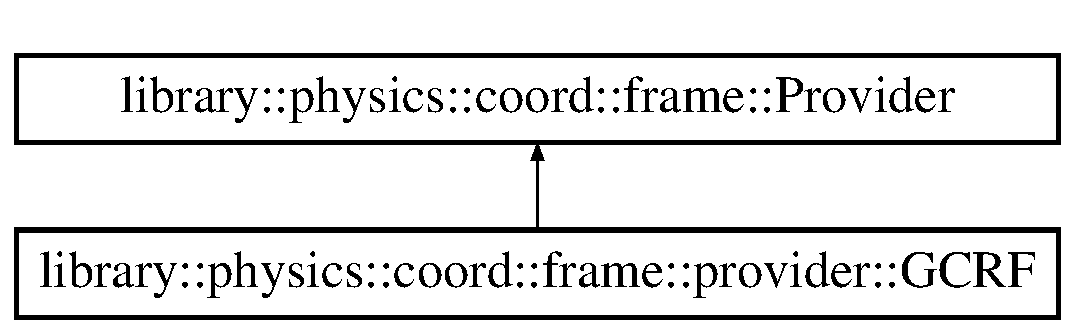
\includegraphics[height=2.000000cm]{classlibrary_1_1physics_1_1coord_1_1frame_1_1provider_1_1_g_c_r_f}
\end{center}
\end{figure}
\subsection*{Public Member Functions}
\begin{DoxyCompactItemize}
\item 
\hyperlink{classlibrary_1_1physics_1_1coord_1_1frame_1_1provider_1_1_g_c_r_f_abdfc6b33e7fa8b1bb8ebb43433c965d4}{G\+C\+RF} ()
\item 
virtual \hyperlink{classlibrary_1_1physics_1_1coord_1_1frame_1_1provider_1_1_g_c_r_f_a03afcfed40d923e0d14e53182331af9c}{$\sim$\+G\+C\+RF} () override
\item 
virtual \hyperlink{classlibrary_1_1physics_1_1coord_1_1frame_1_1provider_1_1_g_c_r_f}{G\+C\+RF} $\ast$ \hyperlink{classlibrary_1_1physics_1_1coord_1_1frame_1_1provider_1_1_g_c_r_f_ae32853b62bfe251fd48262b7ab383fc7}{clone} () const override
\item 
virtual bool \hyperlink{classlibrary_1_1physics_1_1coord_1_1frame_1_1provider_1_1_g_c_r_f_a0e6155c096ff1c231b14e59544fe038c}{is\+Defined} () const override
\item 
virtual \hyperlink{classlibrary_1_1physics_1_1coord_1_1_transform}{Transform} \hyperlink{classlibrary_1_1physics_1_1coord_1_1frame_1_1provider_1_1_g_c_r_f_a4929dae3032a650b74b77b0d0b9bcaaa}{get\+Transform\+At} (const \hyperlink{classlibrary_1_1physics_1_1time_1_1_instant}{Instant} \&an\+Instant) const override
\end{DoxyCompactItemize}


\subsection{Detailed Description}
Geocentric Celestial Reference \hyperlink{classlibrary_1_1physics_1_1coord_1_1_frame}{Frame} (\hyperlink{classlibrary_1_1physics_1_1coord_1_1frame_1_1provider_1_1_g_c_r_f}{G\+C\+RF}) provider. 

https\+://en.wikipedia.\+org/wiki/\+Earth-\/centered\+\_\+inertial 

\subsection{Constructor \& Destructor Documentation}
\mbox{\Hypertarget{classlibrary_1_1physics_1_1coord_1_1frame_1_1provider_1_1_g_c_r_f_abdfc6b33e7fa8b1bb8ebb43433c965d4}\label{classlibrary_1_1physics_1_1coord_1_1frame_1_1provider_1_1_g_c_r_f_abdfc6b33e7fa8b1bb8ebb43433c965d4}} 
\index{library\+::physics\+::coord\+::frame\+::provider\+::\+G\+C\+RF@{library\+::physics\+::coord\+::frame\+::provider\+::\+G\+C\+RF}!G\+C\+RF@{G\+C\+RF}}
\index{G\+C\+RF@{G\+C\+RF}!library\+::physics\+::coord\+::frame\+::provider\+::\+G\+C\+RF@{library\+::physics\+::coord\+::frame\+::provider\+::\+G\+C\+RF}}
\subsubsection{\texorpdfstring{G\+C\+R\+F()}{GCRF()}}
{\footnotesize\ttfamily library\+::physics\+::coord\+::frame\+::provider\+::\+G\+C\+R\+F\+::\+G\+C\+RF (\begin{DoxyParamCaption}{ }\end{DoxyParamCaption})}

\mbox{\Hypertarget{classlibrary_1_1physics_1_1coord_1_1frame_1_1provider_1_1_g_c_r_f_a03afcfed40d923e0d14e53182331af9c}\label{classlibrary_1_1physics_1_1coord_1_1frame_1_1provider_1_1_g_c_r_f_a03afcfed40d923e0d14e53182331af9c}} 
\index{library\+::physics\+::coord\+::frame\+::provider\+::\+G\+C\+RF@{library\+::physics\+::coord\+::frame\+::provider\+::\+G\+C\+RF}!````~G\+C\+RF@{$\sim$\+G\+C\+RF}}
\index{````~G\+C\+RF@{$\sim$\+G\+C\+RF}!library\+::physics\+::coord\+::frame\+::provider\+::\+G\+C\+RF@{library\+::physics\+::coord\+::frame\+::provider\+::\+G\+C\+RF}}
\subsubsection{\texorpdfstring{$\sim$\+G\+C\+R\+F()}{~GCRF()}}
{\footnotesize\ttfamily library\+::physics\+::coord\+::frame\+::provider\+::\+G\+C\+R\+F\+::$\sim$\+G\+C\+RF (\begin{DoxyParamCaption}{ }\end{DoxyParamCaption})\hspace{0.3cm}{\ttfamily [override]}, {\ttfamily [virtual]}}



\subsection{Member Function Documentation}
\mbox{\Hypertarget{classlibrary_1_1physics_1_1coord_1_1frame_1_1provider_1_1_g_c_r_f_ae32853b62bfe251fd48262b7ab383fc7}\label{classlibrary_1_1physics_1_1coord_1_1frame_1_1provider_1_1_g_c_r_f_ae32853b62bfe251fd48262b7ab383fc7}} 
\index{library\+::physics\+::coord\+::frame\+::provider\+::\+G\+C\+RF@{library\+::physics\+::coord\+::frame\+::provider\+::\+G\+C\+RF}!clone@{clone}}
\index{clone@{clone}!library\+::physics\+::coord\+::frame\+::provider\+::\+G\+C\+RF@{library\+::physics\+::coord\+::frame\+::provider\+::\+G\+C\+RF}}
\subsubsection{\texorpdfstring{clone()}{clone()}}
{\footnotesize\ttfamily \hyperlink{classlibrary_1_1physics_1_1coord_1_1frame_1_1provider_1_1_g_c_r_f}{G\+C\+RF} $\ast$ library\+::physics\+::coord\+::frame\+::provider\+::\+G\+C\+R\+F\+::clone (\begin{DoxyParamCaption}{ }\end{DoxyParamCaption}) const\hspace{0.3cm}{\ttfamily [override]}, {\ttfamily [virtual]}}



Implements \hyperlink{classlibrary_1_1physics_1_1coord_1_1frame_1_1_provider_ab8eee40c8ef4aee0b57bedf458f4934e}{library\+::physics\+::coord\+::frame\+::\+Provider}.

\mbox{\Hypertarget{classlibrary_1_1physics_1_1coord_1_1frame_1_1provider_1_1_g_c_r_f_a4929dae3032a650b74b77b0d0b9bcaaa}\label{classlibrary_1_1physics_1_1coord_1_1frame_1_1provider_1_1_g_c_r_f_a4929dae3032a650b74b77b0d0b9bcaaa}} 
\index{library\+::physics\+::coord\+::frame\+::provider\+::\+G\+C\+RF@{library\+::physics\+::coord\+::frame\+::provider\+::\+G\+C\+RF}!get\+Transform\+At@{get\+Transform\+At}}
\index{get\+Transform\+At@{get\+Transform\+At}!library\+::physics\+::coord\+::frame\+::provider\+::\+G\+C\+RF@{library\+::physics\+::coord\+::frame\+::provider\+::\+G\+C\+RF}}
\subsubsection{\texorpdfstring{get\+Transform\+At()}{getTransformAt()}}
{\footnotesize\ttfamily \hyperlink{classlibrary_1_1physics_1_1coord_1_1_transform}{Transform} library\+::physics\+::coord\+::frame\+::provider\+::\+G\+C\+R\+F\+::get\+Transform\+At (\begin{DoxyParamCaption}\item[{const \hyperlink{classlibrary_1_1physics_1_1time_1_1_instant}{Instant} \&}]{an\+Instant }\end{DoxyParamCaption}) const\hspace{0.3cm}{\ttfamily [override]}, {\ttfamily [virtual]}}



Implements \hyperlink{classlibrary_1_1physics_1_1coord_1_1frame_1_1_provider_a796fd2dd337f1304a0e9acf573ce2550}{library\+::physics\+::coord\+::frame\+::\+Provider}.

\mbox{\Hypertarget{classlibrary_1_1physics_1_1coord_1_1frame_1_1provider_1_1_g_c_r_f_a0e6155c096ff1c231b14e59544fe038c}\label{classlibrary_1_1physics_1_1coord_1_1frame_1_1provider_1_1_g_c_r_f_a0e6155c096ff1c231b14e59544fe038c}} 
\index{library\+::physics\+::coord\+::frame\+::provider\+::\+G\+C\+RF@{library\+::physics\+::coord\+::frame\+::provider\+::\+G\+C\+RF}!is\+Defined@{is\+Defined}}
\index{is\+Defined@{is\+Defined}!library\+::physics\+::coord\+::frame\+::provider\+::\+G\+C\+RF@{library\+::physics\+::coord\+::frame\+::provider\+::\+G\+C\+RF}}
\subsubsection{\texorpdfstring{is\+Defined()}{isDefined()}}
{\footnotesize\ttfamily bool library\+::physics\+::coord\+::frame\+::provider\+::\+G\+C\+R\+F\+::is\+Defined (\begin{DoxyParamCaption}{ }\end{DoxyParamCaption}) const\hspace{0.3cm}{\ttfamily [override]}, {\ttfamily [virtual]}}



Implements \hyperlink{classlibrary_1_1physics_1_1coord_1_1frame_1_1_provider_ae7cd093febf2b20f71400f9f79442774}{library\+::physics\+::coord\+::frame\+::\+Provider}.



The documentation for this class was generated from the following files\+:\begin{DoxyCompactItemize}
\item 
include/\+Library/\+Physics/\+Coordinate/\+Frame/\+Providers/\hyperlink{_g_c_r_f_8hpp}{G\+C\+R\+F.\+hpp}\item 
src/\+Library/\+Physics/\+Coordinate/\+Frame/\+Providers/\hyperlink{_g_c_r_f_8cpp}{G\+C\+R\+F.\+cpp}\end{DoxyCompactItemize}

\hypertarget{classlibrary_1_1physics_1_1env_1_1object_1_1_geometry}{}\section{library\+:\+:physics\+:\+:env\+:\+:object\+:\+:Geometry Class Reference}
\label{classlibrary_1_1physics_1_1env_1_1object_1_1_geometry}\index{library\+::physics\+::env\+::object\+::\+Geometry@{library\+::physics\+::env\+::object\+::\+Geometry}}


{\ttfamily \#include $<$Geometry.\+hpp$>$}

\subsection*{Public Types}
\begin{DoxyCompactItemize}
\item 
typedef math\+::geom\+::d3\+::\+Object \hyperlink{classlibrary_1_1physics_1_1env_1_1object_1_1_geometry_a4889a934df09768235fa2d89d0b0b0d6}{Object}
\end{DoxyCompactItemize}
\subsection*{Public Member Functions}
\begin{DoxyCompactItemize}
\item 
\hyperlink{classlibrary_1_1physics_1_1env_1_1object_1_1_geometry_a150ec4f85fe2c76471833df4145b96e8}{Geometry} (const \hyperlink{classlibrary_1_1physics_1_1env_1_1object_1_1_geometry_a4889a934df09768235fa2d89d0b0b0d6}{Geometry\+::\+Object} \&an\+Object, const Shared$<$ const \hyperlink{classlibrary_1_1physics_1_1coord_1_1_frame}{Frame} $>$ \&a\+Frame\+S\+Ptr)
\begin{DoxyCompactList}\small\item\em Constructor. \end{DoxyCompactList}\item 
\hyperlink{classlibrary_1_1physics_1_1env_1_1object_1_1_geometry_a66d7f144c0dba376b52dc37b417691ef}{Geometry} (const Composite \&a\+Composite, const Shared$<$ const \hyperlink{classlibrary_1_1physics_1_1coord_1_1_frame}{Frame} $>$ \&a\+Frame\+S\+Ptr)
\begin{DoxyCompactList}\small\item\em Constructor. \end{DoxyCompactList}\item 
\hyperlink{classlibrary_1_1physics_1_1env_1_1object_1_1_geometry_ae686db5e0a555caf7636596a4b96495c}{Geometry} (const \hyperlink{classlibrary_1_1physics_1_1env_1_1object_1_1_geometry}{Geometry} \&a\+Geometry)
\begin{DoxyCompactList}\small\item\em Copy constructor. \end{DoxyCompactList}\item 
\hyperlink{classlibrary_1_1physics_1_1env_1_1object_1_1_geometry}{Geometry} \& \hyperlink{classlibrary_1_1physics_1_1env_1_1object_1_1_geometry_ac2c0d8cbdf9a6828fdd05024fc6ddad7}{operator=} (const \hyperlink{classlibrary_1_1physics_1_1env_1_1object_1_1_geometry}{Geometry} \&a\+Geometry)
\begin{DoxyCompactList}\small\item\em Copy assignment operator. \end{DoxyCompactList}\item 
bool \hyperlink{classlibrary_1_1physics_1_1env_1_1object_1_1_geometry_a30698963aff142ce94be27205e4ace24}{operator==} (const \hyperlink{classlibrary_1_1physics_1_1env_1_1object_1_1_geometry}{Geometry} \&a\+Geometry) const
\begin{DoxyCompactList}\small\item\em Equal to operator. \end{DoxyCompactList}\item 
bool \hyperlink{classlibrary_1_1physics_1_1env_1_1object_1_1_geometry_aab7132adf31bf6bd03dcdad46b767765}{operator!=} (const \hyperlink{classlibrary_1_1physics_1_1env_1_1object_1_1_geometry}{Geometry} \&a\+Geometry) const
\begin{DoxyCompactList}\small\item\em Not equal to operator. \end{DoxyCompactList}\item 
bool \hyperlink{classlibrary_1_1physics_1_1env_1_1object_1_1_geometry_a1db567a9a36c4b6878e2d59a633f5a38}{is\+Defined} () const
\begin{DoxyCompactList}\small\item\em Check if geometry is defined. \end{DoxyCompactList}\item 
bool \hyperlink{classlibrary_1_1physics_1_1env_1_1object_1_1_geometry_ac750e2584bc1564fbf1daf57a2231a5a}{intersects} (const \hyperlink{classlibrary_1_1physics_1_1env_1_1object_1_1_geometry}{Geometry} \&a\+Geometry) const
\begin{DoxyCompactList}\small\item\em Check if geometry intersects another geometry. \end{DoxyCompactList}\item 
bool \hyperlink{classlibrary_1_1physics_1_1env_1_1object_1_1_geometry_a9122be6cc4de97bb7aec4ad66bee823d}{contains} (const \hyperlink{classlibrary_1_1physics_1_1env_1_1object_1_1_geometry}{Geometry} \&a\+Geometry) const
\begin{DoxyCompactList}\small\item\em Check if geometry contains another geometry. \end{DoxyCompactList}\item 
const Composite \& \hyperlink{classlibrary_1_1physics_1_1env_1_1object_1_1_geometry_ac107f01b791d7844e434c553643dcdf3}{access\+Composite} () const
\begin{DoxyCompactList}\small\item\em Access composite. \end{DoxyCompactList}\item 
Shared$<$ const \hyperlink{classlibrary_1_1physics_1_1coord_1_1_frame}{Frame} $>$ \hyperlink{classlibrary_1_1physics_1_1env_1_1object_1_1_geometry_a1a0569b5cdfba033d355057e215e22b8}{access\+Frame} () const
\begin{DoxyCompactList}\small\item\em Access frame. \end{DoxyCompactList}\item 
\hyperlink{classlibrary_1_1physics_1_1env_1_1object_1_1_geometry}{Geometry} \hyperlink{classlibrary_1_1physics_1_1env_1_1object_1_1_geometry_a3538be01a00bf3aae3c1fbc0e7f4fb6b}{in} (const Shared$<$ const \hyperlink{classlibrary_1_1physics_1_1coord_1_1_frame}{Frame} $>$ \&a\+Frame\+S\+Ptr, const \hyperlink{classlibrary_1_1physics_1_1time_1_1_instant}{Instant} \&an\+Instant) const
\begin{DoxyCompactList}\small\item\em Get geometry expressed in a given frame. \end{DoxyCompactList}\item 
\hyperlink{classlibrary_1_1physics_1_1env_1_1object_1_1_geometry}{Geometry} \hyperlink{classlibrary_1_1physics_1_1env_1_1object_1_1_geometry_a2fccc85beb614199e87a44546c397f7c}{intersection\+With} (const \hyperlink{classlibrary_1_1physics_1_1env_1_1object_1_1_geometry}{Geometry} \&a\+Geometry) const
\begin{DoxyCompactList}\small\item\em Compute intersection of geometry with another geometry. \end{DoxyCompactList}\end{DoxyCompactItemize}
\subsection*{Static Public Member Functions}
\begin{DoxyCompactItemize}
\item 
static \hyperlink{classlibrary_1_1physics_1_1env_1_1object_1_1_geometry}{Geometry} \hyperlink{classlibrary_1_1physics_1_1env_1_1object_1_1_geometry_a5e02f2d9a9a6ac2686f49780811d0fe2}{Undefined} ()
\begin{DoxyCompactList}\small\item\em Constructs an undefined geometry. \end{DoxyCompactList}\end{DoxyCompactItemize}
\subsection*{Friends}
\begin{DoxyCompactItemize}
\item 
std\+::ostream \& \hyperlink{classlibrary_1_1physics_1_1env_1_1object_1_1_geometry_aebfe5b9b5d8cd3dd8a2cfd140a1df583}{operator$<$$<$} (std\+::ostream \&an\+Output\+Stream, const \hyperlink{classlibrary_1_1physics_1_1env_1_1object_1_1_geometry}{Geometry} \&a\+Geometry)
\begin{DoxyCompactList}\small\item\em Output stream operator. \end{DoxyCompactList}\end{DoxyCompactItemize}


\subsection{Member Typedef Documentation}
\mbox{\Hypertarget{classlibrary_1_1physics_1_1env_1_1object_1_1_geometry_a4889a934df09768235fa2d89d0b0b0d6}\label{classlibrary_1_1physics_1_1env_1_1object_1_1_geometry_a4889a934df09768235fa2d89d0b0b0d6}} 
\index{library\+::physics\+::env\+::object\+::\+Geometry@{library\+::physics\+::env\+::object\+::\+Geometry}!Object@{Object}}
\index{Object@{Object}!library\+::physics\+::env\+::object\+::\+Geometry@{library\+::physics\+::env\+::object\+::\+Geometry}}
\subsubsection{\texorpdfstring{Object}{Object}}
{\footnotesize\ttfamily typedef math\+::geom\+::d3\+::\+Object \hyperlink{classlibrary_1_1physics_1_1env_1_1object_1_1_geometry_a4889a934df09768235fa2d89d0b0b0d6}{library\+::physics\+::env\+::object\+::\+Geometry\+::\+Object}}



\subsection{Constructor \& Destructor Documentation}
\mbox{\Hypertarget{classlibrary_1_1physics_1_1env_1_1object_1_1_geometry_a150ec4f85fe2c76471833df4145b96e8}\label{classlibrary_1_1physics_1_1env_1_1object_1_1_geometry_a150ec4f85fe2c76471833df4145b96e8}} 
\index{library\+::physics\+::env\+::object\+::\+Geometry@{library\+::physics\+::env\+::object\+::\+Geometry}!Geometry@{Geometry}}
\index{Geometry@{Geometry}!library\+::physics\+::env\+::object\+::\+Geometry@{library\+::physics\+::env\+::object\+::\+Geometry}}
\subsubsection{\texorpdfstring{Geometry()}{Geometry()}\hspace{0.1cm}{\footnotesize\ttfamily [1/3]}}
{\footnotesize\ttfamily library\+::physics\+::env\+::object\+::\+Geometry\+::\+Geometry (\begin{DoxyParamCaption}\item[{const \hyperlink{classlibrary_1_1physics_1_1env_1_1object_1_1_geometry_a4889a934df09768235fa2d89d0b0b0d6}{Geometry\+::\+Object} \&}]{an\+Object,  }\item[{const Shared$<$ const \hyperlink{classlibrary_1_1physics_1_1coord_1_1_frame}{Frame} $>$ \&}]{a\+Frame\+S\+Ptr }\end{DoxyParamCaption})}



Constructor. 


\begin{DoxyParams}[1]{Parameters}
\mbox{\tt in}  & {\em an\+Object} & An object \\
\hline
\mbox{\tt in}  & {\em a\+Frame\+S\+Ptr} & A shared pointer to frame \\
\hline
\end{DoxyParams}
\mbox{\Hypertarget{classlibrary_1_1physics_1_1env_1_1object_1_1_geometry_a66d7f144c0dba376b52dc37b417691ef}\label{classlibrary_1_1physics_1_1env_1_1object_1_1_geometry_a66d7f144c0dba376b52dc37b417691ef}} 
\index{library\+::physics\+::env\+::object\+::\+Geometry@{library\+::physics\+::env\+::object\+::\+Geometry}!Geometry@{Geometry}}
\index{Geometry@{Geometry}!library\+::physics\+::env\+::object\+::\+Geometry@{library\+::physics\+::env\+::object\+::\+Geometry}}
\subsubsection{\texorpdfstring{Geometry()}{Geometry()}\hspace{0.1cm}{\footnotesize\ttfamily [2/3]}}
{\footnotesize\ttfamily library\+::physics\+::env\+::object\+::\+Geometry\+::\+Geometry (\begin{DoxyParamCaption}\item[{const Composite \&}]{a\+Composite,  }\item[{const Shared$<$ const \hyperlink{classlibrary_1_1physics_1_1coord_1_1_frame}{Frame} $>$ \&}]{a\+Frame\+S\+Ptr }\end{DoxyParamCaption})}



Constructor. 


\begin{DoxyParams}[1]{Parameters}
\mbox{\tt in}  & {\em a\+Composite} & A composite \\
\hline
\mbox{\tt in}  & {\em a\+Frame\+S\+Ptr} & A shared pointer to frame \\
\hline
\end{DoxyParams}
\mbox{\Hypertarget{classlibrary_1_1physics_1_1env_1_1object_1_1_geometry_ae686db5e0a555caf7636596a4b96495c}\label{classlibrary_1_1physics_1_1env_1_1object_1_1_geometry_ae686db5e0a555caf7636596a4b96495c}} 
\index{library\+::physics\+::env\+::object\+::\+Geometry@{library\+::physics\+::env\+::object\+::\+Geometry}!Geometry@{Geometry}}
\index{Geometry@{Geometry}!library\+::physics\+::env\+::object\+::\+Geometry@{library\+::physics\+::env\+::object\+::\+Geometry}}
\subsubsection{\texorpdfstring{Geometry()}{Geometry()}\hspace{0.1cm}{\footnotesize\ttfamily [3/3]}}
{\footnotesize\ttfamily library\+::physics\+::env\+::object\+::\+Geometry\+::\+Geometry (\begin{DoxyParamCaption}\item[{const \hyperlink{classlibrary_1_1physics_1_1env_1_1object_1_1_geometry}{Geometry} \&}]{a\+Geometry }\end{DoxyParamCaption})}



Copy constructor. 


\begin{DoxyParams}[1]{Parameters}
\mbox{\tt in}  & {\em a\+Geometry} & A geometry \\
\hline
\end{DoxyParams}


\subsection{Member Function Documentation}
\mbox{\Hypertarget{classlibrary_1_1physics_1_1env_1_1object_1_1_geometry_ac107f01b791d7844e434c553643dcdf3}\label{classlibrary_1_1physics_1_1env_1_1object_1_1_geometry_ac107f01b791d7844e434c553643dcdf3}} 
\index{library\+::physics\+::env\+::object\+::\+Geometry@{library\+::physics\+::env\+::object\+::\+Geometry}!access\+Composite@{access\+Composite}}
\index{access\+Composite@{access\+Composite}!library\+::physics\+::env\+::object\+::\+Geometry@{library\+::physics\+::env\+::object\+::\+Geometry}}
\subsubsection{\texorpdfstring{access\+Composite()}{accessComposite()}}
{\footnotesize\ttfamily const Composite \& library\+::physics\+::env\+::object\+::\+Geometry\+::access\+Composite (\begin{DoxyParamCaption}{ }\end{DoxyParamCaption}) const}



Access composite. 

\begin{DoxyReturn}{Returns}
Reference to composite 
\end{DoxyReturn}
\mbox{\Hypertarget{classlibrary_1_1physics_1_1env_1_1object_1_1_geometry_a1a0569b5cdfba033d355057e215e22b8}\label{classlibrary_1_1physics_1_1env_1_1object_1_1_geometry_a1a0569b5cdfba033d355057e215e22b8}} 
\index{library\+::physics\+::env\+::object\+::\+Geometry@{library\+::physics\+::env\+::object\+::\+Geometry}!access\+Frame@{access\+Frame}}
\index{access\+Frame@{access\+Frame}!library\+::physics\+::env\+::object\+::\+Geometry@{library\+::physics\+::env\+::object\+::\+Geometry}}
\subsubsection{\texorpdfstring{access\+Frame()}{accessFrame()}}
{\footnotesize\ttfamily Shared$<$ const \hyperlink{classlibrary_1_1physics_1_1coord_1_1_frame}{Frame} $>$ library\+::physics\+::env\+::object\+::\+Geometry\+::access\+Frame (\begin{DoxyParamCaption}{ }\end{DoxyParamCaption}) const}



Access frame. 

\begin{DoxyReturn}{Returns}
Shared pointer to frame 
\end{DoxyReturn}
\mbox{\Hypertarget{classlibrary_1_1physics_1_1env_1_1object_1_1_geometry_a9122be6cc4de97bb7aec4ad66bee823d}\label{classlibrary_1_1physics_1_1env_1_1object_1_1_geometry_a9122be6cc4de97bb7aec4ad66bee823d}} 
\index{library\+::physics\+::env\+::object\+::\+Geometry@{library\+::physics\+::env\+::object\+::\+Geometry}!contains@{contains}}
\index{contains@{contains}!library\+::physics\+::env\+::object\+::\+Geometry@{library\+::physics\+::env\+::object\+::\+Geometry}}
\subsubsection{\texorpdfstring{contains()}{contains()}}
{\footnotesize\ttfamily bool library\+::physics\+::env\+::object\+::\+Geometry\+::contains (\begin{DoxyParamCaption}\item[{const \hyperlink{classlibrary_1_1physics_1_1env_1_1object_1_1_geometry}{Geometry} \&}]{a\+Geometry }\end{DoxyParamCaption}) const}



Check if geometry contains another geometry. 


\begin{DoxyParams}[1]{Parameters}
\mbox{\tt in}  & {\em a\+Geometry} & A geometry \\
\hline
\end{DoxyParams}
\begin{DoxyReturn}{Returns}
True if geometry contains another geometry 
\end{DoxyReturn}
\mbox{\Hypertarget{classlibrary_1_1physics_1_1env_1_1object_1_1_geometry_a3538be01a00bf3aae3c1fbc0e7f4fb6b}\label{classlibrary_1_1physics_1_1env_1_1object_1_1_geometry_a3538be01a00bf3aae3c1fbc0e7f4fb6b}} 
\index{library\+::physics\+::env\+::object\+::\+Geometry@{library\+::physics\+::env\+::object\+::\+Geometry}!in@{in}}
\index{in@{in}!library\+::physics\+::env\+::object\+::\+Geometry@{library\+::physics\+::env\+::object\+::\+Geometry}}
\subsubsection{\texorpdfstring{in()}{in()}}
{\footnotesize\ttfamily \hyperlink{classlibrary_1_1physics_1_1env_1_1object_1_1_geometry}{Geometry} library\+::physics\+::env\+::object\+::\+Geometry\+::in (\begin{DoxyParamCaption}\item[{const Shared$<$ const \hyperlink{classlibrary_1_1physics_1_1coord_1_1_frame}{Frame} $>$ \&}]{a\+Frame\+S\+Ptr,  }\item[{const \hyperlink{classlibrary_1_1physics_1_1time_1_1_instant}{Instant} \&}]{an\+Instant }\end{DoxyParamCaption}) const}



Get geometry expressed in a given frame. 


\begin{DoxyParams}[1]{Parameters}
\mbox{\tt in}  & {\em a\+Frame\+S\+Ptr} & A shared pointer to frame \\
\hline
\mbox{\tt in}  & {\em an\+Instant} & An instant \\
\hline
\end{DoxyParams}
\begin{DoxyReturn}{Returns}
\hyperlink{classlibrary_1_1physics_1_1env_1_1object_1_1_geometry}{Geometry} expressed in a given frame 
\end{DoxyReturn}
\mbox{\Hypertarget{classlibrary_1_1physics_1_1env_1_1object_1_1_geometry_a2fccc85beb614199e87a44546c397f7c}\label{classlibrary_1_1physics_1_1env_1_1object_1_1_geometry_a2fccc85beb614199e87a44546c397f7c}} 
\index{library\+::physics\+::env\+::object\+::\+Geometry@{library\+::physics\+::env\+::object\+::\+Geometry}!intersection\+With@{intersection\+With}}
\index{intersection\+With@{intersection\+With}!library\+::physics\+::env\+::object\+::\+Geometry@{library\+::physics\+::env\+::object\+::\+Geometry}}
\subsubsection{\texorpdfstring{intersection\+With()}{intersectionWith()}}
{\footnotesize\ttfamily \hyperlink{classlibrary_1_1physics_1_1env_1_1object_1_1_geometry}{Geometry} library\+::physics\+::env\+::object\+::\+Geometry\+::intersection\+With (\begin{DoxyParamCaption}\item[{const \hyperlink{classlibrary_1_1physics_1_1env_1_1object_1_1_geometry}{Geometry} \&}]{a\+Geometry }\end{DoxyParamCaption}) const}



Compute intersection of geometry with another geometry. 


\begin{DoxyParams}[1]{Parameters}
\mbox{\tt in}  & {\em a\+Geometry} & A geometry \\
\hline
\end{DoxyParams}
\begin{DoxyReturn}{Returns}
Intersection of geometry with another geometry 
\end{DoxyReturn}
\mbox{\Hypertarget{classlibrary_1_1physics_1_1env_1_1object_1_1_geometry_ac750e2584bc1564fbf1daf57a2231a5a}\label{classlibrary_1_1physics_1_1env_1_1object_1_1_geometry_ac750e2584bc1564fbf1daf57a2231a5a}} 
\index{library\+::physics\+::env\+::object\+::\+Geometry@{library\+::physics\+::env\+::object\+::\+Geometry}!intersects@{intersects}}
\index{intersects@{intersects}!library\+::physics\+::env\+::object\+::\+Geometry@{library\+::physics\+::env\+::object\+::\+Geometry}}
\subsubsection{\texorpdfstring{intersects()}{intersects()}}
{\footnotesize\ttfamily bool library\+::physics\+::env\+::object\+::\+Geometry\+::intersects (\begin{DoxyParamCaption}\item[{const \hyperlink{classlibrary_1_1physics_1_1env_1_1object_1_1_geometry}{Geometry} \&}]{a\+Geometry }\end{DoxyParamCaption}) const}



Check if geometry intersects another geometry. 


\begin{DoxyParams}[1]{Parameters}
\mbox{\tt in}  & {\em a\+Geometry} & A geometry \\
\hline
\end{DoxyParams}
\begin{DoxyReturn}{Returns}
True if geometry intersects another geometry 
\end{DoxyReturn}
\mbox{\Hypertarget{classlibrary_1_1physics_1_1env_1_1object_1_1_geometry_a1db567a9a36c4b6878e2d59a633f5a38}\label{classlibrary_1_1physics_1_1env_1_1object_1_1_geometry_a1db567a9a36c4b6878e2d59a633f5a38}} 
\index{library\+::physics\+::env\+::object\+::\+Geometry@{library\+::physics\+::env\+::object\+::\+Geometry}!is\+Defined@{is\+Defined}}
\index{is\+Defined@{is\+Defined}!library\+::physics\+::env\+::object\+::\+Geometry@{library\+::physics\+::env\+::object\+::\+Geometry}}
\subsubsection{\texorpdfstring{is\+Defined()}{isDefined()}}
{\footnotesize\ttfamily bool library\+::physics\+::env\+::object\+::\+Geometry\+::is\+Defined (\begin{DoxyParamCaption}{ }\end{DoxyParamCaption}) const}



Check if geometry is defined. 

\begin{DoxyReturn}{Returns}
True if geometry is defined 
\end{DoxyReturn}
\mbox{\Hypertarget{classlibrary_1_1physics_1_1env_1_1object_1_1_geometry_aab7132adf31bf6bd03dcdad46b767765}\label{classlibrary_1_1physics_1_1env_1_1object_1_1_geometry_aab7132adf31bf6bd03dcdad46b767765}} 
\index{library\+::physics\+::env\+::object\+::\+Geometry@{library\+::physics\+::env\+::object\+::\+Geometry}!operator"!=@{operator"!=}}
\index{operator"!=@{operator"!=}!library\+::physics\+::env\+::object\+::\+Geometry@{library\+::physics\+::env\+::object\+::\+Geometry}}
\subsubsection{\texorpdfstring{operator"!=()}{operator!=()}}
{\footnotesize\ttfamily bool library\+::physics\+::env\+::object\+::\+Geometry\+::operator!= (\begin{DoxyParamCaption}\item[{const \hyperlink{classlibrary_1_1physics_1_1env_1_1object_1_1_geometry}{Geometry} \&}]{a\+Geometry }\end{DoxyParamCaption}) const}



Not equal to operator. 


\begin{DoxyParams}[1]{Parameters}
\mbox{\tt in}  & {\em a\+Geometry} & A geometry \\
\hline
\end{DoxyParams}
\begin{DoxyReturn}{Returns}
True if geometries are not equal 
\end{DoxyReturn}
\mbox{\Hypertarget{classlibrary_1_1physics_1_1env_1_1object_1_1_geometry_ac2c0d8cbdf9a6828fdd05024fc6ddad7}\label{classlibrary_1_1physics_1_1env_1_1object_1_1_geometry_ac2c0d8cbdf9a6828fdd05024fc6ddad7}} 
\index{library\+::physics\+::env\+::object\+::\+Geometry@{library\+::physics\+::env\+::object\+::\+Geometry}!operator=@{operator=}}
\index{operator=@{operator=}!library\+::physics\+::env\+::object\+::\+Geometry@{library\+::physics\+::env\+::object\+::\+Geometry}}
\subsubsection{\texorpdfstring{operator=()}{operator=()}}
{\footnotesize\ttfamily \hyperlink{classlibrary_1_1physics_1_1env_1_1object_1_1_geometry}{Geometry} \& library\+::physics\+::env\+::object\+::\+Geometry\+::operator= (\begin{DoxyParamCaption}\item[{const \hyperlink{classlibrary_1_1physics_1_1env_1_1object_1_1_geometry}{Geometry} \&}]{a\+Geometry }\end{DoxyParamCaption})}



Copy assignment operator. 


\begin{DoxyParams}[1]{Parameters}
\mbox{\tt in}  & {\em a\+Geometry} & A geometry \\
\hline
\end{DoxyParams}
\begin{DoxyReturn}{Returns}
Reference to geometry 
\end{DoxyReturn}
\mbox{\Hypertarget{classlibrary_1_1physics_1_1env_1_1object_1_1_geometry_a30698963aff142ce94be27205e4ace24}\label{classlibrary_1_1physics_1_1env_1_1object_1_1_geometry_a30698963aff142ce94be27205e4ace24}} 
\index{library\+::physics\+::env\+::object\+::\+Geometry@{library\+::physics\+::env\+::object\+::\+Geometry}!operator==@{operator==}}
\index{operator==@{operator==}!library\+::physics\+::env\+::object\+::\+Geometry@{library\+::physics\+::env\+::object\+::\+Geometry}}
\subsubsection{\texorpdfstring{operator==()}{operator==()}}
{\footnotesize\ttfamily bool library\+::physics\+::env\+::object\+::\+Geometry\+::operator== (\begin{DoxyParamCaption}\item[{const \hyperlink{classlibrary_1_1physics_1_1env_1_1object_1_1_geometry}{Geometry} \&}]{a\+Geometry }\end{DoxyParamCaption}) const}



Equal to operator. 


\begin{DoxyParams}[1]{Parameters}
\mbox{\tt in}  & {\em a\+Geometry} & A geometry \\
\hline
\end{DoxyParams}
\begin{DoxyReturn}{Returns}
True if geometries are equal 
\end{DoxyReturn}
\mbox{\Hypertarget{classlibrary_1_1physics_1_1env_1_1object_1_1_geometry_a5e02f2d9a9a6ac2686f49780811d0fe2}\label{classlibrary_1_1physics_1_1env_1_1object_1_1_geometry_a5e02f2d9a9a6ac2686f49780811d0fe2}} 
\index{library\+::physics\+::env\+::object\+::\+Geometry@{library\+::physics\+::env\+::object\+::\+Geometry}!Undefined@{Undefined}}
\index{Undefined@{Undefined}!library\+::physics\+::env\+::object\+::\+Geometry@{library\+::physics\+::env\+::object\+::\+Geometry}}
\subsubsection{\texorpdfstring{Undefined()}{Undefined()}}
{\footnotesize\ttfamily \hyperlink{classlibrary_1_1physics_1_1env_1_1object_1_1_geometry}{Geometry} library\+::physics\+::env\+::object\+::\+Geometry\+::\+Undefined (\begin{DoxyParamCaption}{ }\end{DoxyParamCaption})\hspace{0.3cm}{\ttfamily [static]}}



Constructs an undefined geometry. 


\begin{DoxyCode}
\hyperlink{classlibrary_1_1physics_1_1env_1_1object_1_1_geometry_a150ec4f85fe2c76471833df4145b96e8}{Geometry} geometry = \hyperlink{classlibrary_1_1physics_1_1env_1_1object_1_1_geometry_a5e02f2d9a9a6ac2686f49780811d0fe2}{Geometry::Undefined}() ; \textcolor{comment}{// Undefined}
\end{DoxyCode}


\begin{DoxyReturn}{Returns}
Undefined geometry 
\end{DoxyReturn}


\subsection{Friends And Related Function Documentation}
\mbox{\Hypertarget{classlibrary_1_1physics_1_1env_1_1object_1_1_geometry_aebfe5b9b5d8cd3dd8a2cfd140a1df583}\label{classlibrary_1_1physics_1_1env_1_1object_1_1_geometry_aebfe5b9b5d8cd3dd8a2cfd140a1df583}} 
\index{library\+::physics\+::env\+::object\+::\+Geometry@{library\+::physics\+::env\+::object\+::\+Geometry}!operator$<$$<$@{operator$<$$<$}}
\index{operator$<$$<$@{operator$<$$<$}!library\+::physics\+::env\+::object\+::\+Geometry@{library\+::physics\+::env\+::object\+::\+Geometry}}
\subsubsection{\texorpdfstring{operator$<$$<$}{operator<<}}
{\footnotesize\ttfamily std\+::ostream\& operator$<$$<$ (\begin{DoxyParamCaption}\item[{std\+::ostream \&}]{an\+Output\+Stream,  }\item[{const \hyperlink{classlibrary_1_1physics_1_1env_1_1object_1_1_geometry}{Geometry} \&}]{a\+Geometry }\end{DoxyParamCaption})\hspace{0.3cm}{\ttfamily [friend]}}



Output stream operator. 


\begin{DoxyParams}[1]{Parameters}
\mbox{\tt in}  & {\em an\+Output\+Stream} & An output stream \\
\hline
\mbox{\tt in}  & {\em a\+Geometry} & A geometry \\
\hline
\end{DoxyParams}
\begin{DoxyReturn}{Returns}
A reference to output stream 
\end{DoxyReturn}


The documentation for this class was generated from the following files\+:\begin{DoxyCompactItemize}
\item 
include/\+Library/\+Physics/\+Environment/\+Object/\hyperlink{_geometry_8hpp}{Geometry.\+hpp}\item 
src/\+Library/\+Physics/\+Environment/\+Object/\hyperlink{_geometry_8cpp}{Geometry.\+cpp}\end{DoxyCompactItemize}

\hypertarget{classlibrary_1_1physics_1_1coord_1_1frame_1_1provider_1_1_i_c_r_f}{}\section{library\+:\+:physics\+:\+:coord\+:\+:frame\+:\+:provider\+:\+:I\+C\+RF Class Reference}
\label{classlibrary_1_1physics_1_1coord_1_1frame_1_1provider_1_1_i_c_r_f}\index{library\+::physics\+::coord\+::frame\+::provider\+::\+I\+C\+RF@{library\+::physics\+::coord\+::frame\+::provider\+::\+I\+C\+RF}}


International Celestial Reference \hyperlink{classlibrary_1_1physics_1_1coord_1_1_frame}{Frame} (\hyperlink{classlibrary_1_1physics_1_1coord_1_1frame_1_1provider_1_1_i_c_r_f}{I\+C\+RF}) provider.  




{\ttfamily \#include $<$I\+C\+R\+F.\+hpp$>$}

Inheritance diagram for library\+:\+:physics\+:\+:coord\+:\+:frame\+:\+:provider\+:\+:I\+C\+RF\+:\begin{figure}[H]
\begin{center}
\leavevmode
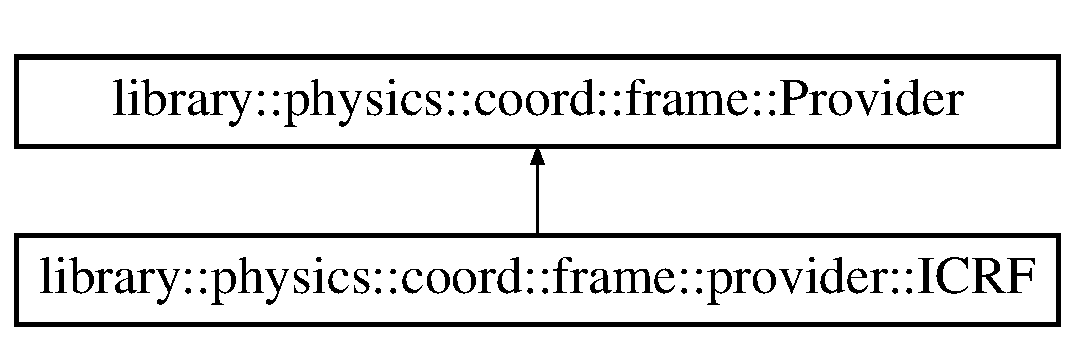
\includegraphics[height=2.000000cm]{classlibrary_1_1physics_1_1coord_1_1frame_1_1provider_1_1_i_c_r_f}
\end{center}
\end{figure}
\subsection*{Public Member Functions}
\begin{DoxyCompactItemize}
\item 
\hyperlink{classlibrary_1_1physics_1_1coord_1_1frame_1_1provider_1_1_i_c_r_f_a65d0457c6b892f83b14fa6f31eea0410}{I\+C\+RF} ()
\item 
virtual \hyperlink{classlibrary_1_1physics_1_1coord_1_1frame_1_1provider_1_1_i_c_r_f_a60159943ae7b049f5295d5ed656c4b78}{$\sim$\+I\+C\+RF} () override
\item 
virtual \hyperlink{classlibrary_1_1physics_1_1coord_1_1frame_1_1provider_1_1_i_c_r_f}{I\+C\+RF} $\ast$ \hyperlink{classlibrary_1_1physics_1_1coord_1_1frame_1_1provider_1_1_i_c_r_f_a06ce5c7c4bc22045d612d951cbeb4d14}{clone} () const override
\item 
virtual bool \hyperlink{classlibrary_1_1physics_1_1coord_1_1frame_1_1provider_1_1_i_c_r_f_a533e5d0240150b5c23080ee8bf89d040}{is\+Defined} () const override
\item 
virtual \hyperlink{classlibrary_1_1physics_1_1coord_1_1_transform}{Transform} \hyperlink{classlibrary_1_1physics_1_1coord_1_1frame_1_1provider_1_1_i_c_r_f_a6f5256cac7e8f7b1e947a9f6627a9a33}{get\+Transform\+At} (const \hyperlink{classlibrary_1_1physics_1_1time_1_1_instant}{Instant} \&an\+Instant) const override
\end{DoxyCompactItemize}


\subsection{Detailed Description}
International Celestial Reference \hyperlink{classlibrary_1_1physics_1_1coord_1_1_frame}{Frame} (\hyperlink{classlibrary_1_1physics_1_1coord_1_1frame_1_1provider_1_1_i_c_r_f}{I\+C\+RF}) provider. 

https\+://en.wikipedia.\+org/wiki/\+International\+\_\+\+Celestial\+\_\+\+Reference\+\_\+\+Frame 

\subsection{Constructor \& Destructor Documentation}
\mbox{\Hypertarget{classlibrary_1_1physics_1_1coord_1_1frame_1_1provider_1_1_i_c_r_f_a65d0457c6b892f83b14fa6f31eea0410}\label{classlibrary_1_1physics_1_1coord_1_1frame_1_1provider_1_1_i_c_r_f_a65d0457c6b892f83b14fa6f31eea0410}} 
\index{library\+::physics\+::coord\+::frame\+::provider\+::\+I\+C\+RF@{library\+::physics\+::coord\+::frame\+::provider\+::\+I\+C\+RF}!I\+C\+RF@{I\+C\+RF}}
\index{I\+C\+RF@{I\+C\+RF}!library\+::physics\+::coord\+::frame\+::provider\+::\+I\+C\+RF@{library\+::physics\+::coord\+::frame\+::provider\+::\+I\+C\+RF}}
\subsubsection{\texorpdfstring{I\+C\+R\+F()}{ICRF()}}
{\footnotesize\ttfamily library\+::physics\+::coord\+::frame\+::provider\+::\+I\+C\+R\+F\+::\+I\+C\+RF (\begin{DoxyParamCaption}{ }\end{DoxyParamCaption})}

\mbox{\Hypertarget{classlibrary_1_1physics_1_1coord_1_1frame_1_1provider_1_1_i_c_r_f_a60159943ae7b049f5295d5ed656c4b78}\label{classlibrary_1_1physics_1_1coord_1_1frame_1_1provider_1_1_i_c_r_f_a60159943ae7b049f5295d5ed656c4b78}} 
\index{library\+::physics\+::coord\+::frame\+::provider\+::\+I\+C\+RF@{library\+::physics\+::coord\+::frame\+::provider\+::\+I\+C\+RF}!````~I\+C\+RF@{$\sim$\+I\+C\+RF}}
\index{````~I\+C\+RF@{$\sim$\+I\+C\+RF}!library\+::physics\+::coord\+::frame\+::provider\+::\+I\+C\+RF@{library\+::physics\+::coord\+::frame\+::provider\+::\+I\+C\+RF}}
\subsubsection{\texorpdfstring{$\sim$\+I\+C\+R\+F()}{~ICRF()}}
{\footnotesize\ttfamily library\+::physics\+::coord\+::frame\+::provider\+::\+I\+C\+R\+F\+::$\sim$\+I\+C\+RF (\begin{DoxyParamCaption}{ }\end{DoxyParamCaption})\hspace{0.3cm}{\ttfamily [override]}, {\ttfamily [virtual]}}



\subsection{Member Function Documentation}
\mbox{\Hypertarget{classlibrary_1_1physics_1_1coord_1_1frame_1_1provider_1_1_i_c_r_f_a06ce5c7c4bc22045d612d951cbeb4d14}\label{classlibrary_1_1physics_1_1coord_1_1frame_1_1provider_1_1_i_c_r_f_a06ce5c7c4bc22045d612d951cbeb4d14}} 
\index{library\+::physics\+::coord\+::frame\+::provider\+::\+I\+C\+RF@{library\+::physics\+::coord\+::frame\+::provider\+::\+I\+C\+RF}!clone@{clone}}
\index{clone@{clone}!library\+::physics\+::coord\+::frame\+::provider\+::\+I\+C\+RF@{library\+::physics\+::coord\+::frame\+::provider\+::\+I\+C\+RF}}
\subsubsection{\texorpdfstring{clone()}{clone()}}
{\footnotesize\ttfamily \hyperlink{classlibrary_1_1physics_1_1coord_1_1frame_1_1provider_1_1_i_c_r_f}{I\+C\+RF} $\ast$ library\+::physics\+::coord\+::frame\+::provider\+::\+I\+C\+R\+F\+::clone (\begin{DoxyParamCaption}{ }\end{DoxyParamCaption}) const\hspace{0.3cm}{\ttfamily [override]}, {\ttfamily [virtual]}}



Implements \hyperlink{classlibrary_1_1physics_1_1coord_1_1frame_1_1_provider_ab8eee40c8ef4aee0b57bedf458f4934e}{library\+::physics\+::coord\+::frame\+::\+Provider}.

\mbox{\Hypertarget{classlibrary_1_1physics_1_1coord_1_1frame_1_1provider_1_1_i_c_r_f_a6f5256cac7e8f7b1e947a9f6627a9a33}\label{classlibrary_1_1physics_1_1coord_1_1frame_1_1provider_1_1_i_c_r_f_a6f5256cac7e8f7b1e947a9f6627a9a33}} 
\index{library\+::physics\+::coord\+::frame\+::provider\+::\+I\+C\+RF@{library\+::physics\+::coord\+::frame\+::provider\+::\+I\+C\+RF}!get\+Transform\+At@{get\+Transform\+At}}
\index{get\+Transform\+At@{get\+Transform\+At}!library\+::physics\+::coord\+::frame\+::provider\+::\+I\+C\+RF@{library\+::physics\+::coord\+::frame\+::provider\+::\+I\+C\+RF}}
\subsubsection{\texorpdfstring{get\+Transform\+At()}{getTransformAt()}}
{\footnotesize\ttfamily \hyperlink{classlibrary_1_1physics_1_1coord_1_1_transform}{Transform} library\+::physics\+::coord\+::frame\+::provider\+::\+I\+C\+R\+F\+::get\+Transform\+At (\begin{DoxyParamCaption}\item[{const \hyperlink{classlibrary_1_1physics_1_1time_1_1_instant}{Instant} \&}]{an\+Instant }\end{DoxyParamCaption}) const\hspace{0.3cm}{\ttfamily [override]}, {\ttfamily [virtual]}}



Implements \hyperlink{classlibrary_1_1physics_1_1coord_1_1frame_1_1_provider_a796fd2dd337f1304a0e9acf573ce2550}{library\+::physics\+::coord\+::frame\+::\+Provider}.

\mbox{\Hypertarget{classlibrary_1_1physics_1_1coord_1_1frame_1_1provider_1_1_i_c_r_f_a533e5d0240150b5c23080ee8bf89d040}\label{classlibrary_1_1physics_1_1coord_1_1frame_1_1provider_1_1_i_c_r_f_a533e5d0240150b5c23080ee8bf89d040}} 
\index{library\+::physics\+::coord\+::frame\+::provider\+::\+I\+C\+RF@{library\+::physics\+::coord\+::frame\+::provider\+::\+I\+C\+RF}!is\+Defined@{is\+Defined}}
\index{is\+Defined@{is\+Defined}!library\+::physics\+::coord\+::frame\+::provider\+::\+I\+C\+RF@{library\+::physics\+::coord\+::frame\+::provider\+::\+I\+C\+RF}}
\subsubsection{\texorpdfstring{is\+Defined()}{isDefined()}}
{\footnotesize\ttfamily bool library\+::physics\+::coord\+::frame\+::provider\+::\+I\+C\+R\+F\+::is\+Defined (\begin{DoxyParamCaption}{ }\end{DoxyParamCaption}) const\hspace{0.3cm}{\ttfamily [override]}, {\ttfamily [virtual]}}



Implements \hyperlink{classlibrary_1_1physics_1_1coord_1_1frame_1_1_provider_ae7cd093febf2b20f71400f9f79442774}{library\+::physics\+::coord\+::frame\+::\+Provider}.



The documentation for this class was generated from the following files\+:\begin{DoxyCompactItemize}
\item 
include/\+Library/\+Physics/\+Coordinate/\+Frame/\+Providers/\hyperlink{_i_c_r_f_8hpp}{I\+C\+R\+F.\+hpp}\item 
src/\+Library/\+Physics/\+Coordinate/\+Frame/\+Providers/\hyperlink{_i_c_r_f_8cpp}{I\+C\+R\+F.\+cpp}\end{DoxyCompactItemize}

\hypertarget{classlibrary_1_1physics_1_1time_1_1_instant}{}\section{library\+:\+:physics\+:\+:time\+:\+:Instant Class Reference}
\label{classlibrary_1_1physics_1_1time_1_1_instant}\index{library\+::physics\+::time\+::\+Instant@{library\+::physics\+::time\+::\+Instant}}


Point in time.  




{\ttfamily \#include $<$Instant.\+hpp$>$}

\subsection*{Public Member Functions}
\begin{DoxyCompactItemize}
\item 
\hyperlink{classlibrary_1_1physics_1_1time_1_1_instant_a7916a9d8acb9de4eda35f9d72086a618}{Instant} ()=delete
\begin{DoxyCompactList}\small\item\em Default constructor (deleted) \end{DoxyCompactList}\item 
bool \hyperlink{classlibrary_1_1physics_1_1time_1_1_instant_ab948da61d082b526741348e55547b1b7}{operator==} (const \hyperlink{classlibrary_1_1physics_1_1time_1_1_instant}{Instant} \&an\+Instant) const
\begin{DoxyCompactList}\small\item\em Equal to operator. \end{DoxyCompactList}\item 
bool \hyperlink{classlibrary_1_1physics_1_1time_1_1_instant_a1d055c15365cc75756e6a85040e1ae04}{operator!=} (const \hyperlink{classlibrary_1_1physics_1_1time_1_1_instant}{Instant} \&an\+Instant) const
\begin{DoxyCompactList}\small\item\em Not equal to operator. \end{DoxyCompactList}\item 
bool \hyperlink{classlibrary_1_1physics_1_1time_1_1_instant_a6b211c85f6eaa9c5122c068280a65878}{operator$<$} (const \hyperlink{classlibrary_1_1physics_1_1time_1_1_instant}{Instant} \&an\+Instant) const
\begin{DoxyCompactList}\small\item\em Less than operator. \end{DoxyCompactList}\item 
bool \hyperlink{classlibrary_1_1physics_1_1time_1_1_instant_a44bc09a2eb633bbb08b240dd886402ee}{operator$<$=} (const \hyperlink{classlibrary_1_1physics_1_1time_1_1_instant}{Instant} \&an\+Instant) const
\begin{DoxyCompactList}\small\item\em Less than or equal to operator. \end{DoxyCompactList}\item 
bool \hyperlink{classlibrary_1_1physics_1_1time_1_1_instant_ad9ddedc5a5ce3d69894577dbd34bb6ce}{operator$>$} (const \hyperlink{classlibrary_1_1physics_1_1time_1_1_instant}{Instant} \&an\+Instant) const
\begin{DoxyCompactList}\small\item\em Greater than operator. \end{DoxyCompactList}\item 
bool \hyperlink{classlibrary_1_1physics_1_1time_1_1_instant_a025f5f159e2a7fb0320c3e0d55cff341}{operator$>$=} (const \hyperlink{classlibrary_1_1physics_1_1time_1_1_instant}{Instant} \&an\+Instant) const
\begin{DoxyCompactList}\small\item\em Greater than operator. \end{DoxyCompactList}\item 
\hyperlink{classlibrary_1_1physics_1_1time_1_1_instant}{Instant} \hyperlink{classlibrary_1_1physics_1_1time_1_1_instant_afa8c43afa94b882543c64e9610ccdc61}{operator+} (const \hyperlink{classlibrary_1_1physics_1_1time_1_1_duration}{Duration} \&a\+Duration) const
\begin{DoxyCompactList}\small\item\em Addition operator. \end{DoxyCompactList}\item 
\hyperlink{classlibrary_1_1physics_1_1time_1_1_instant}{Instant} \hyperlink{classlibrary_1_1physics_1_1time_1_1_instant_a7b64292c796d6c54bfab311a1e13735f}{operator-\/} (const \hyperlink{classlibrary_1_1physics_1_1time_1_1_duration}{Duration} \&a\+Duration) const
\begin{DoxyCompactList}\small\item\em Subtraction operator. \end{DoxyCompactList}\item 
\hyperlink{classlibrary_1_1physics_1_1time_1_1_duration}{Duration} \hyperlink{classlibrary_1_1physics_1_1time_1_1_instant_a913a30067f54516382a5ea6548d2a16d}{operator-\/} (const \hyperlink{classlibrary_1_1physics_1_1time_1_1_instant}{Instant} \&an\+Instant) const
\begin{DoxyCompactList}\small\item\em Subtraction operator. \end{DoxyCompactList}\item 
\hyperlink{classlibrary_1_1physics_1_1time_1_1_instant}{Instant} \& \hyperlink{classlibrary_1_1physics_1_1time_1_1_instant_a91febb93e31d68b4fe02910f0dbfa365}{operator+=} (const \hyperlink{classlibrary_1_1physics_1_1time_1_1_duration}{Duration} \&a\+Duration)
\begin{DoxyCompactList}\small\item\em Addition assignement operator. \end{DoxyCompactList}\item 
\hyperlink{classlibrary_1_1physics_1_1time_1_1_instant}{Instant} \& \hyperlink{classlibrary_1_1physics_1_1time_1_1_instant_a629531fc4507a3ef0375f88696fed34e}{operator-\/=} (const \hyperlink{classlibrary_1_1physics_1_1time_1_1_duration}{Duration} \&a\+Duration)
\begin{DoxyCompactList}\small\item\em Subtraction assignement operator. \end{DoxyCompactList}\item 
bool \hyperlink{classlibrary_1_1physics_1_1time_1_1_instant_aaef81e773a2d3059612b0d99dc7cf661}{is\+Defined} () const
\begin{DoxyCompactList}\small\item\em Check if instant is defined. \end{DoxyCompactList}\item 
bool \hyperlink{classlibrary_1_1physics_1_1time_1_1_instant_a649a2505c26b68b17ed7a80429b599ee}{is\+Post\+Epoch} () const
\begin{DoxyCompactList}\small\item\em Check if instant is post-\/epoch (J2000) \end{DoxyCompactList}\item 
\hyperlink{classlibrary_1_1physics_1_1time_1_1_date_time}{time\+::\+Date\+Time} \hyperlink{classlibrary_1_1physics_1_1time_1_1_instant_ae40dbe983c197c961c0cf5aceefa352c}{get\+Date\+Time} (const \hyperlink{namespacelibrary_1_1physics_1_1time_a09d2bc9fbc7b0b5f92e1419bd655e6bb}{Scale} \&a\+Time\+Scale) const
\begin{DoxyCompactList}\small\item\em Get date-\/time expressed in given time scale. \end{DoxyCompactList}\item 
Real \hyperlink{classlibrary_1_1physics_1_1time_1_1_instant_a592844ceab80e29ab65766aedc194acb}{get\+Julian\+Date} (const \hyperlink{namespacelibrary_1_1physics_1_1time_a09d2bc9fbc7b0b5f92e1419bd655e6bb}{Scale} \&a\+Time\+Scale) const
\begin{DoxyCompactList}\small\item\em Get Julian \hyperlink{classlibrary_1_1physics_1_1time_1_1_date}{Date} expressed in given time scale. \end{DoxyCompactList}\item 
Real \hyperlink{classlibrary_1_1physics_1_1time_1_1_instant_a01a167d6aee17d47ff200b2472199382}{get\+Modified\+Julian\+Date} (const \hyperlink{namespacelibrary_1_1physics_1_1time_a09d2bc9fbc7b0b5f92e1419bd655e6bb}{Scale} \&a\+Time\+Scale) const
\begin{DoxyCompactList}\small\item\em Get Modified Julian \hyperlink{classlibrary_1_1physics_1_1time_1_1_date}{Date} expressed in given time scale. \end{DoxyCompactList}\item 
String \hyperlink{classlibrary_1_1physics_1_1time_1_1_instant_aa3e7ee2c6704053afbf7ed142bb40c4e}{to\+String} (const \hyperlink{namespacelibrary_1_1physics_1_1time_a09d2bc9fbc7b0b5f92e1419bd655e6bb}{Scale} \&a\+Time\+Scale=\hyperlink{namespacelibrary_1_1physics_1_1time_a09d2bc9fbc7b0b5f92e1419bd655e6bba9234324ddf6b4176b57d803a925b7961}{Scale\+::\+U\+TC}) const
\begin{DoxyCompactList}\small\item\em Get string representation of instant. \end{DoxyCompactList}\end{DoxyCompactItemize}
\subsection*{Static Public Member Functions}
\begin{DoxyCompactItemize}
\item 
static \hyperlink{classlibrary_1_1physics_1_1time_1_1_instant}{Instant} \hyperlink{classlibrary_1_1physics_1_1time_1_1_instant_aae55667866c1d0c4a94650673c6b712c}{Undefined} ()
\begin{DoxyCompactList}\small\item\em Constructs an undefined instant. \end{DoxyCompactList}\item 
static \hyperlink{classlibrary_1_1physics_1_1time_1_1_instant}{Instant} \hyperlink{classlibrary_1_1physics_1_1time_1_1_instant_abdee2ddacb34859a3be2a4cf97c4af81}{Now} ()
\begin{DoxyCompactList}\small\item\em Constructs an instant at current time. \end{DoxyCompactList}\item 
static \hyperlink{classlibrary_1_1physics_1_1time_1_1_instant}{Instant} \hyperlink{classlibrary_1_1physics_1_1time_1_1_instant_a2a4f57aa71693b8def06788d55bc3bd3}{J2000} ()
\begin{DoxyCompactList}\small\item\em Constructs instant at J2000 epoch. \end{DoxyCompactList}\item 
static \hyperlink{classlibrary_1_1physics_1_1time_1_1_instant}{Instant} \hyperlink{classlibrary_1_1physics_1_1time_1_1_instant_ac827b6ffa57ce75a3c56c462d4c872f8}{Date\+Time} (const \hyperlink{classlibrary_1_1physics_1_1time_1_1_date_time}{time\+::\+Date\+Time} \&a\+Date\+Time, const \hyperlink{namespacelibrary_1_1physics_1_1time_a09d2bc9fbc7b0b5f92e1419bd655e6bb}{Scale} \&a\+Time\+Scale)
\begin{DoxyCompactList}\small\item\em Constructs instant from date-\/time. \end{DoxyCompactList}\item 
static \hyperlink{classlibrary_1_1physics_1_1time_1_1_instant}{Instant} \hyperlink{classlibrary_1_1physics_1_1time_1_1_instant_a06f5e092a3a5ee126c9521c12e349d56}{Julian\+Date} (const Real \&a\+Julian\+Date, const \hyperlink{namespacelibrary_1_1physics_1_1time_a09d2bc9fbc7b0b5f92e1419bd655e6bb}{Scale} \&a\+Time\+Scale)
\begin{DoxyCompactList}\small\item\em Constructs instant from Julian \hyperlink{classlibrary_1_1physics_1_1time_1_1_date}{Date}. \end{DoxyCompactList}\item 
static \hyperlink{classlibrary_1_1physics_1_1time_1_1_instant}{Instant} \hyperlink{classlibrary_1_1physics_1_1time_1_1_instant_a800d784f67ed5eaa6432b71f4534a170}{Modified\+Julian\+Date} (const Real \&a\+Modified\+Julian\+Date, const \hyperlink{namespacelibrary_1_1physics_1_1time_a09d2bc9fbc7b0b5f92e1419bd655e6bb}{Scale} \&a\+Time\+Scale)
\begin{DoxyCompactList}\small\item\em Constructs instant from Modified Julian \hyperlink{classlibrary_1_1physics_1_1time_1_1_date}{Date}. \end{DoxyCompactList}\end{DoxyCompactItemize}
\subsection*{Friends}
\begin{DoxyCompactItemize}
\item 
std\+::ostream \& \hyperlink{classlibrary_1_1physics_1_1time_1_1_instant_a01668796f6ebfd8c23c2d0df17f00b65}{operator$<$$<$} (std\+::ostream \&an\+Output\+Stream, const \hyperlink{classlibrary_1_1physics_1_1time_1_1_instant}{Instant} \&an\+Instant)
\begin{DoxyCompactList}\small\item\em Output stream operator. \end{DoxyCompactList}\end{DoxyCompactItemize}


\subsection{Detailed Description}
Point in time. 

https\+://en.wikipedia.\+org/wiki/\+Instant https\+://www.boost.\+org/doc/libs/1\+\_\+67\+\_\+0/doc/html/date\+\_\+time/details.html\+::date\+\_\+time.\+calculations http\+://rhodesmill.org/skyfield/time.\+html http\+://www.madore.\+org/$\sim$david/computers/unix-\/leap-\/seconds.html http\+://help.agi.\+com/\+A\+G\+I\+Components\+Java/html/\+Time\+And\+Time\+Standards.htm 

\subsection{Constructor \& Destructor Documentation}
\mbox{\Hypertarget{classlibrary_1_1physics_1_1time_1_1_instant_a7916a9d8acb9de4eda35f9d72086a618}\label{classlibrary_1_1physics_1_1time_1_1_instant_a7916a9d8acb9de4eda35f9d72086a618}} 
\index{library\+::physics\+::time\+::\+Instant@{library\+::physics\+::time\+::\+Instant}!Instant@{Instant}}
\index{Instant@{Instant}!library\+::physics\+::time\+::\+Instant@{library\+::physics\+::time\+::\+Instant}}
\subsubsection{\texorpdfstring{Instant()}{Instant()}}
{\footnotesize\ttfamily library\+::physics\+::time\+::\+Instant\+::\+Instant (\begin{DoxyParamCaption}{ }\end{DoxyParamCaption})\hspace{0.3cm}{\ttfamily [delete]}}



Default constructor (deleted) 



\subsection{Member Function Documentation}
\mbox{\Hypertarget{classlibrary_1_1physics_1_1time_1_1_instant_ac827b6ffa57ce75a3c56c462d4c872f8}\label{classlibrary_1_1physics_1_1time_1_1_instant_ac827b6ffa57ce75a3c56c462d4c872f8}} 
\index{library\+::physics\+::time\+::\+Instant@{library\+::physics\+::time\+::\+Instant}!Date\+Time@{Date\+Time}}
\index{Date\+Time@{Date\+Time}!library\+::physics\+::time\+::\+Instant@{library\+::physics\+::time\+::\+Instant}}
\subsubsection{\texorpdfstring{Date\+Time()}{DateTime()}}
{\footnotesize\ttfamily \hyperlink{classlibrary_1_1physics_1_1time_1_1_instant}{Instant} library\+::physics\+::time\+::\+Instant\+::\+Date\+Time (\begin{DoxyParamCaption}\item[{const \hyperlink{classlibrary_1_1physics_1_1time_1_1_date_time}{time\+::\+Date\+Time} \&}]{a\+Date\+Time,  }\item[{const \hyperlink{namespacelibrary_1_1physics_1_1time_a09d2bc9fbc7b0b5f92e1419bd655e6bb}{Scale} \&}]{a\+Time\+Scale }\end{DoxyParamCaption})\hspace{0.3cm}{\ttfamily [static]}}



Constructs instant from date-\/time. 


\begin{DoxyCode}
\hyperlink{classlibrary_1_1physics_1_1time_1_1_instant_a7916a9d8acb9de4eda35f9d72086a618}{Instant} instant = \hyperlink{classlibrary_1_1physics_1_1time_1_1_instant_ac827b6ffa57ce75a3c56c462d4c872f8}{Instant::DateTime}(\hyperlink{classlibrary_1_1physics_1_1time_1_1_instant_ac827b6ffa57ce75a3c56c462d4c872f8}{DateTime}(2000, 1, 1, 12, 0, 0), 
      \hyperlink{namespacelibrary_1_1physics_1_1time_a09d2bc9fbc7b0b5f92e1419bd655e6bbadf1f3edb9115acb0a1e04209b7a9937b}{Scale::TT}) ; \textcolor{comment}{// 2000-01-01 12:00:00 [TT]}
\end{DoxyCode}


\mbox{[}in\mbox{]} a\+Date\+Time A date-\/time  \mbox{[}in\mbox{]} a\+Time\+Scale A time scale \begin{DoxyReturn}{Returns}
\hyperlink{classlibrary_1_1physics_1_1time_1_1_instant}{Instant} 
\end{DoxyReturn}
\mbox{\Hypertarget{classlibrary_1_1physics_1_1time_1_1_instant_ae40dbe983c197c961c0cf5aceefa352c}\label{classlibrary_1_1physics_1_1time_1_1_instant_ae40dbe983c197c961c0cf5aceefa352c}} 
\index{library\+::physics\+::time\+::\+Instant@{library\+::physics\+::time\+::\+Instant}!get\+Date\+Time@{get\+Date\+Time}}
\index{get\+Date\+Time@{get\+Date\+Time}!library\+::physics\+::time\+::\+Instant@{library\+::physics\+::time\+::\+Instant}}
\subsubsection{\texorpdfstring{get\+Date\+Time()}{getDateTime()}}
{\footnotesize\ttfamily \hyperlink{classlibrary_1_1physics_1_1time_1_1_date_time}{time\+::\+Date\+Time} library\+::physics\+::time\+::\+Instant\+::get\+Date\+Time (\begin{DoxyParamCaption}\item[{const \hyperlink{namespacelibrary_1_1physics_1_1time_a09d2bc9fbc7b0b5f92e1419bd655e6bb}{Scale} \&}]{a\+Time\+Scale }\end{DoxyParamCaption}) const}



Get date-\/time expressed in given time scale. 


\begin{DoxyCode}
\hyperlink{classlibrary_1_1physics_1_1time_1_1_instant_a2a4f57aa71693b8def06788d55bc3bd3}{Instant::J2000}().\hyperlink{classlibrary_1_1physics_1_1time_1_1_instant_ae40dbe983c197c961c0cf5aceefa352c}{getDateTime}(\hyperlink{namespacelibrary_1_1physics_1_1time_a09d2bc9fbc7b0b5f92e1419bd655e6bbadf1f3edb9115acb0a1e04209b7a9937b}{Scale::TT}) ; \textcolor{comment}{// 2000-01-01 12:00:00}
\end{DoxyCode}



\begin{DoxyParams}[1]{Parameters}
\mbox{\tt in}  & {\em a\+Time\+Scale} & A time scale \\
\hline
\end{DoxyParams}
\begin{DoxyReturn}{Returns}
Date-\/time 
\end{DoxyReturn}
\mbox{\Hypertarget{classlibrary_1_1physics_1_1time_1_1_instant_a592844ceab80e29ab65766aedc194acb}\label{classlibrary_1_1physics_1_1time_1_1_instant_a592844ceab80e29ab65766aedc194acb}} 
\index{library\+::physics\+::time\+::\+Instant@{library\+::physics\+::time\+::\+Instant}!get\+Julian\+Date@{get\+Julian\+Date}}
\index{get\+Julian\+Date@{get\+Julian\+Date}!library\+::physics\+::time\+::\+Instant@{library\+::physics\+::time\+::\+Instant}}
\subsubsection{\texorpdfstring{get\+Julian\+Date()}{getJulianDate()}}
{\footnotesize\ttfamily Real library\+::physics\+::time\+::\+Instant\+::get\+Julian\+Date (\begin{DoxyParamCaption}\item[{const \hyperlink{namespacelibrary_1_1physics_1_1time_a09d2bc9fbc7b0b5f92e1419bd655e6bb}{Scale} \&}]{a\+Time\+Scale }\end{DoxyParamCaption}) const}



Get Julian \hyperlink{classlibrary_1_1physics_1_1time_1_1_date}{Date} expressed in given time scale. 


\begin{DoxyCode}
\hyperlink{classlibrary_1_1physics_1_1time_1_1_instant_a2a4f57aa71693b8def06788d55bc3bd3}{Instant::J2000}().\hyperlink{classlibrary_1_1physics_1_1time_1_1_instant_a592844ceab80e29ab65766aedc194acb}{getJulianDate}(\hyperlink{namespacelibrary_1_1physics_1_1time_a09d2bc9fbc7b0b5f92e1419bd655e6bbadf1f3edb9115acb0a1e04209b7a9937b}{Scale::TT}) ; \textcolor{comment}{// 2451545.0}
\end{DoxyCode}



\begin{DoxyParams}[1]{Parameters}
\mbox{\tt in}  & {\em a\+Time\+Scale} & A time scale \\
\hline
\end{DoxyParams}
\begin{DoxyReturn}{Returns}
Julian \hyperlink{classlibrary_1_1physics_1_1time_1_1_date}{Date} 
\end{DoxyReturn}
\mbox{\Hypertarget{classlibrary_1_1physics_1_1time_1_1_instant_a01a167d6aee17d47ff200b2472199382}\label{classlibrary_1_1physics_1_1time_1_1_instant_a01a167d6aee17d47ff200b2472199382}} 
\index{library\+::physics\+::time\+::\+Instant@{library\+::physics\+::time\+::\+Instant}!get\+Modified\+Julian\+Date@{get\+Modified\+Julian\+Date}}
\index{get\+Modified\+Julian\+Date@{get\+Modified\+Julian\+Date}!library\+::physics\+::time\+::\+Instant@{library\+::physics\+::time\+::\+Instant}}
\subsubsection{\texorpdfstring{get\+Modified\+Julian\+Date()}{getModifiedJulianDate()}}
{\footnotesize\ttfamily Real library\+::physics\+::time\+::\+Instant\+::get\+Modified\+Julian\+Date (\begin{DoxyParamCaption}\item[{const \hyperlink{namespacelibrary_1_1physics_1_1time_a09d2bc9fbc7b0b5f92e1419bd655e6bb}{Scale} \&}]{a\+Time\+Scale }\end{DoxyParamCaption}) const}



Get Modified Julian \hyperlink{classlibrary_1_1physics_1_1time_1_1_date}{Date} expressed in given time scale. 


\begin{DoxyCode}
\hyperlink{classlibrary_1_1physics_1_1time_1_1_instant_a2a4f57aa71693b8def06788d55bc3bd3}{Instant::J2000}().\hyperlink{classlibrary_1_1physics_1_1time_1_1_instant_a01a167d6aee17d47ff200b2472199382}{getModifiedJulianDate}(
      \hyperlink{namespacelibrary_1_1physics_1_1time_a09d2bc9fbc7b0b5f92e1419bd655e6bbadf1f3edb9115acb0a1e04209b7a9937b}{Scale::TT}) ; \textcolor{comment}{// 51544.0}
\end{DoxyCode}



\begin{DoxyParams}[1]{Parameters}
\mbox{\tt in}  & {\em a\+Time\+Scale} & A time scale \\
\hline
\end{DoxyParams}
\begin{DoxyReturn}{Returns}
Modified Julian \hyperlink{classlibrary_1_1physics_1_1time_1_1_date}{Date} 
\end{DoxyReturn}
\mbox{\Hypertarget{classlibrary_1_1physics_1_1time_1_1_instant_aaef81e773a2d3059612b0d99dc7cf661}\label{classlibrary_1_1physics_1_1time_1_1_instant_aaef81e773a2d3059612b0d99dc7cf661}} 
\index{library\+::physics\+::time\+::\+Instant@{library\+::physics\+::time\+::\+Instant}!is\+Defined@{is\+Defined}}
\index{is\+Defined@{is\+Defined}!library\+::physics\+::time\+::\+Instant@{library\+::physics\+::time\+::\+Instant}}
\subsubsection{\texorpdfstring{is\+Defined()}{isDefined()}}
{\footnotesize\ttfamily bool library\+::physics\+::time\+::\+Instant\+::is\+Defined (\begin{DoxyParamCaption}{ }\end{DoxyParamCaption}) const}



Check if instant is defined. 


\begin{DoxyCode}
\hyperlink{classlibrary_1_1physics_1_1time_1_1_instant_ac827b6ffa57ce75a3c56c462d4c872f8}{Instant::DateTime}(\hyperlink{classlibrary_1_1physics_1_1time_1_1_instant_ac827b6ffa57ce75a3c56c462d4c872f8}{DateTime}(2018, 1, 1, 0, 0, 0), 
      \hyperlink{namespacelibrary_1_1physics_1_1time_a09d2bc9fbc7b0b5f92e1419bd655e6bba9234324ddf6b4176b57d803a925b7961}{Scale::UTC}).\hyperlink{classlibrary_1_1physics_1_1time_1_1_instant_aaef81e773a2d3059612b0d99dc7cf661}{isDefined}() ; \textcolor{comment}{// True}
\end{DoxyCode}


\begin{DoxyReturn}{Returns}
True if instant is defined 
\end{DoxyReturn}
\mbox{\Hypertarget{classlibrary_1_1physics_1_1time_1_1_instant_a649a2505c26b68b17ed7a80429b599ee}\label{classlibrary_1_1physics_1_1time_1_1_instant_a649a2505c26b68b17ed7a80429b599ee}} 
\index{library\+::physics\+::time\+::\+Instant@{library\+::physics\+::time\+::\+Instant}!is\+Post\+Epoch@{is\+Post\+Epoch}}
\index{is\+Post\+Epoch@{is\+Post\+Epoch}!library\+::physics\+::time\+::\+Instant@{library\+::physics\+::time\+::\+Instant}}
\subsubsection{\texorpdfstring{is\+Post\+Epoch()}{isPostEpoch()}}
{\footnotesize\ttfamily bool library\+::physics\+::time\+::\+Instant\+::is\+Post\+Epoch (\begin{DoxyParamCaption}{ }\end{DoxyParamCaption}) const}



Check if instant is post-\/epoch (J2000) 


\begin{DoxyCode}
\hyperlink{classlibrary_1_1physics_1_1time_1_1_instant_ac827b6ffa57ce75a3c56c462d4c872f8}{Instant::DateTime}(\hyperlink{classlibrary_1_1physics_1_1time_1_1_instant_ac827b6ffa57ce75a3c56c462d4c872f8}{DateTime}(2018, 1, 1, 0, 0, 0), 
      \hyperlink{namespacelibrary_1_1physics_1_1time_a09d2bc9fbc7b0b5f92e1419bd655e6bba9234324ddf6b4176b57d803a925b7961}{Scale::UTC}).\hyperlink{classlibrary_1_1physics_1_1time_1_1_instant_a649a2505c26b68b17ed7a80429b599ee}{isPostEpoch}() ; \textcolor{comment}{// True}
\end{DoxyCode}


\begin{DoxyReturn}{Returns}
True if instant is post-\/epoch 
\end{DoxyReturn}
\mbox{\Hypertarget{classlibrary_1_1physics_1_1time_1_1_instant_a2a4f57aa71693b8def06788d55bc3bd3}\label{classlibrary_1_1physics_1_1time_1_1_instant_a2a4f57aa71693b8def06788d55bc3bd3}} 
\index{library\+::physics\+::time\+::\+Instant@{library\+::physics\+::time\+::\+Instant}!J2000@{J2000}}
\index{J2000@{J2000}!library\+::physics\+::time\+::\+Instant@{library\+::physics\+::time\+::\+Instant}}
\subsubsection{\texorpdfstring{J2000()}{J2000()}}
{\footnotesize\ttfamily \hyperlink{classlibrary_1_1physics_1_1time_1_1_instant}{Instant} library\+::physics\+::time\+::\+Instant\+::\+J2000 (\begin{DoxyParamCaption}{ }\end{DoxyParamCaption})\hspace{0.3cm}{\ttfamily [static]}}



Constructs instant at J2000 epoch. 

The currently-\/used standard epoch \char`\"{}\+J2000\char`\"{} is defined by international agreement to be equivalent to\+:
\begin{DoxyItemize}
\item The Gregorian date January 1, 2000 at 12\+:00 TT (Terrestrial \hyperlink{classlibrary_1_1physics_1_1time_1_1_time}{Time}).
\item The Julian date 2451545.\+0 TT (Terrestrial \hyperlink{classlibrary_1_1physics_1_1time_1_1_time}{Time}).
\item January 1, 2000, 11\+:59\+:27.\+816 T\+AI (International Atomic \hyperlink{classlibrary_1_1physics_1_1time_1_1_time}{Time}).
\item January 1, 2000, 11\+:58\+:55.\+816 U\+TC (Coordinated Universal \hyperlink{classlibrary_1_1physics_1_1time_1_1_time}{Time}).
\end{DoxyItemize}

https\+://en.wikipedia.\+org/wiki/\+Epoch\+\_\+(astronomy)\#\+Julian\+\_\+years\+\_\+and\+\_\+\+J2000

\begin{DoxyReturn}{Returns}
\hyperlink{classlibrary_1_1physics_1_1time_1_1_instant}{Instant} at J2000 epoch 
\end{DoxyReturn}
\mbox{\Hypertarget{classlibrary_1_1physics_1_1time_1_1_instant_a06f5e092a3a5ee126c9521c12e349d56}\label{classlibrary_1_1physics_1_1time_1_1_instant_a06f5e092a3a5ee126c9521c12e349d56}} 
\index{library\+::physics\+::time\+::\+Instant@{library\+::physics\+::time\+::\+Instant}!Julian\+Date@{Julian\+Date}}
\index{Julian\+Date@{Julian\+Date}!library\+::physics\+::time\+::\+Instant@{library\+::physics\+::time\+::\+Instant}}
\subsubsection{\texorpdfstring{Julian\+Date()}{JulianDate()}}
{\footnotesize\ttfamily \hyperlink{classlibrary_1_1physics_1_1time_1_1_instant}{Instant} library\+::physics\+::time\+::\+Instant\+::\+Julian\+Date (\begin{DoxyParamCaption}\item[{const Real \&}]{a\+Julian\+Date,  }\item[{const \hyperlink{namespacelibrary_1_1physics_1_1time_a09d2bc9fbc7b0b5f92e1419bd655e6bb}{Scale} \&}]{a\+Time\+Scale }\end{DoxyParamCaption})\hspace{0.3cm}{\ttfamily [static]}}



Constructs instant from Julian \hyperlink{classlibrary_1_1physics_1_1time_1_1_date}{Date}. 


\begin{DoxyCode}
\hyperlink{classlibrary_1_1physics_1_1time_1_1_instant_a7916a9d8acb9de4eda35f9d72086a618}{Instant} instant = \hyperlink{classlibrary_1_1physics_1_1time_1_1_instant_a06f5e092a3a5ee126c9521c12e349d56}{Instant::JulianDate}(2451545.0, 
      \hyperlink{namespacelibrary_1_1physics_1_1time_a09d2bc9fbc7b0b5f92e1419bd655e6bbadf1f3edb9115acb0a1e04209b7a9937b}{Scale::TT}) ; \textcolor{comment}{// 2000-01-01 12:00:00 [TT]}
\end{DoxyCode}


https\+://en.wikipedia.\+org/wiki/\+Julian\+\_\+day

\mbox{[}in\mbox{]} a\+Julian\+Date A Julian \hyperlink{classlibrary_1_1physics_1_1time_1_1_date}{Date}  \mbox{[}in\mbox{]} a\+Time\+Scale A time scale \begin{DoxyReturn}{Returns}
\hyperlink{classlibrary_1_1physics_1_1time_1_1_instant}{Instant} 
\end{DoxyReturn}
\mbox{\Hypertarget{classlibrary_1_1physics_1_1time_1_1_instant_a800d784f67ed5eaa6432b71f4534a170}\label{classlibrary_1_1physics_1_1time_1_1_instant_a800d784f67ed5eaa6432b71f4534a170}} 
\index{library\+::physics\+::time\+::\+Instant@{library\+::physics\+::time\+::\+Instant}!Modified\+Julian\+Date@{Modified\+Julian\+Date}}
\index{Modified\+Julian\+Date@{Modified\+Julian\+Date}!library\+::physics\+::time\+::\+Instant@{library\+::physics\+::time\+::\+Instant}}
\subsubsection{\texorpdfstring{Modified\+Julian\+Date()}{ModifiedJulianDate()}}
{\footnotesize\ttfamily \hyperlink{classlibrary_1_1physics_1_1time_1_1_instant}{Instant} library\+::physics\+::time\+::\+Instant\+::\+Modified\+Julian\+Date (\begin{DoxyParamCaption}\item[{const Real \&}]{a\+Modified\+Julian\+Date,  }\item[{const \hyperlink{namespacelibrary_1_1physics_1_1time_a09d2bc9fbc7b0b5f92e1419bd655e6bb}{Scale} \&}]{a\+Time\+Scale }\end{DoxyParamCaption})\hspace{0.3cm}{\ttfamily [static]}}



Constructs instant from Modified Julian \hyperlink{classlibrary_1_1physics_1_1time_1_1_date}{Date}. 


\begin{DoxyCode}
\hyperlink{classlibrary_1_1physics_1_1time_1_1_instant_a7916a9d8acb9de4eda35f9d72086a618}{Instant} instant = \hyperlink{classlibrary_1_1physics_1_1time_1_1_instant_a800d784f67ed5eaa6432b71f4534a170}{Instant::ModifiedJulianDate}(51544.0, 
      \hyperlink{namespacelibrary_1_1physics_1_1time_a09d2bc9fbc7b0b5f92e1419bd655e6bbadf1f3edb9115acb0a1e04209b7a9937b}{Scale::TT}) ; \textcolor{comment}{// 2000-01-01 12:00:00 [TT]}
\end{DoxyCode}


https\+://en.wikipedia.\+org/wiki/\+Julian\+\_\+day

\mbox{[}in\mbox{]} a\+Julian\+Date A Modified Julian \hyperlink{classlibrary_1_1physics_1_1time_1_1_date}{Date}  \mbox{[}in\mbox{]} a\+Time\+Scale A time scale \begin{DoxyReturn}{Returns}
\hyperlink{classlibrary_1_1physics_1_1time_1_1_instant}{Instant} 
\end{DoxyReturn}
\mbox{\Hypertarget{classlibrary_1_1physics_1_1time_1_1_instant_abdee2ddacb34859a3be2a4cf97c4af81}\label{classlibrary_1_1physics_1_1time_1_1_instant_abdee2ddacb34859a3be2a4cf97c4af81}} 
\index{library\+::physics\+::time\+::\+Instant@{library\+::physics\+::time\+::\+Instant}!Now@{Now}}
\index{Now@{Now}!library\+::physics\+::time\+::\+Instant@{library\+::physics\+::time\+::\+Instant}}
\subsubsection{\texorpdfstring{Now()}{Now()}}
{\footnotesize\ttfamily \hyperlink{classlibrary_1_1physics_1_1time_1_1_instant}{Instant} library\+::physics\+::time\+::\+Instant\+::\+Now (\begin{DoxyParamCaption}{ }\end{DoxyParamCaption})\hspace{0.3cm}{\ttfamily [static]}}



Constructs an instant at current time. 


\begin{DoxyCode}
\hyperlink{classlibrary_1_1physics_1_1time_1_1_instant_a7916a9d8acb9de4eda35f9d72086a618}{Instant} instant = \hyperlink{classlibrary_1_1physics_1_1time_1_1_instant_abdee2ddacb34859a3be2a4cf97c4af81}{Instant::Now}() ;
\end{DoxyCode}


\begin{DoxyReturn}{Returns}
\hyperlink{classlibrary_1_1physics_1_1time_1_1_instant}{Instant} at current time 
\end{DoxyReturn}
\mbox{\Hypertarget{classlibrary_1_1physics_1_1time_1_1_instant_a1d055c15365cc75756e6a85040e1ae04}\label{classlibrary_1_1physics_1_1time_1_1_instant_a1d055c15365cc75756e6a85040e1ae04}} 
\index{library\+::physics\+::time\+::\+Instant@{library\+::physics\+::time\+::\+Instant}!operator"!=@{operator"!=}}
\index{operator"!=@{operator"!=}!library\+::physics\+::time\+::\+Instant@{library\+::physics\+::time\+::\+Instant}}
\subsubsection{\texorpdfstring{operator"!=()}{operator!=()}}
{\footnotesize\ttfamily bool library\+::physics\+::time\+::\+Instant\+::operator!= (\begin{DoxyParamCaption}\item[{const \hyperlink{classlibrary_1_1physics_1_1time_1_1_instant}{Instant} \&}]{an\+Instant }\end{DoxyParamCaption}) const}



Not equal to operator. 


\begin{DoxyCode}
\hyperlink{classlibrary_1_1physics_1_1time_1_1_instant_ac827b6ffa57ce75a3c56c462d4c872f8}{Instant::DateTime}(\hyperlink{classlibrary_1_1physics_1_1time_1_1_instant_ac827b6ffa57ce75a3c56c462d4c872f8}{DateTime}(2018, 1, 2, 0, 0, 0), 
      \hyperlink{namespacelibrary_1_1physics_1_1time_a09d2bc9fbc7b0b5f92e1419bd655e6bbadf1f3edb9115acb0a1e04209b7a9937b}{Scale::TT}) != \hyperlink{classlibrary_1_1physics_1_1time_1_1_instant_ac827b6ffa57ce75a3c56c462d4c872f8}{Instant::DateTime}(\hyperlink{classlibrary_1_1physics_1_1time_1_1_instant_ac827b6ffa57ce75a3c56c462d4c872f8}{DateTime}(2018, 1, 1, 0, 0, 0), 
      \hyperlink{namespacelibrary_1_1physics_1_1time_a09d2bc9fbc7b0b5f92e1419bd655e6bbadf1f3edb9115acb0a1e04209b7a9937b}{Scale::TT}) ; \textcolor{comment}{// True}
\end{DoxyCode}



\begin{DoxyParams}[1]{Parameters}
\mbox{\tt in}  & {\em an\+Instant} & An instant \\
\hline
\end{DoxyParams}
\begin{DoxyReturn}{Returns}
True if instants are not equal 
\end{DoxyReturn}
\mbox{\Hypertarget{classlibrary_1_1physics_1_1time_1_1_instant_afa8c43afa94b882543c64e9610ccdc61}\label{classlibrary_1_1physics_1_1time_1_1_instant_afa8c43afa94b882543c64e9610ccdc61}} 
\index{library\+::physics\+::time\+::\+Instant@{library\+::physics\+::time\+::\+Instant}!operator+@{operator+}}
\index{operator+@{operator+}!library\+::physics\+::time\+::\+Instant@{library\+::physics\+::time\+::\+Instant}}
\subsubsection{\texorpdfstring{operator+()}{operator+()}}
{\footnotesize\ttfamily \hyperlink{classlibrary_1_1physics_1_1time_1_1_instant}{Instant} library\+::physics\+::time\+::\+Instant\+::operator+ (\begin{DoxyParamCaption}\item[{const \hyperlink{classlibrary_1_1physics_1_1time_1_1_duration}{Duration} \&}]{a\+Duration }\end{DoxyParamCaption}) const}



Addition operator. 


\begin{DoxyCode}
\hyperlink{classlibrary_1_1physics_1_1time_1_1_instant_ac827b6ffa57ce75a3c56c462d4c872f8}{Instant::DateTime}(\hyperlink{classlibrary_1_1physics_1_1time_1_1_instant_ac827b6ffa57ce75a3c56c462d4c872f8}{DateTime}(2018, 1, 1, 0, 0, 0), 
      \hyperlink{namespacelibrary_1_1physics_1_1time_a09d2bc9fbc7b0b5f92e1419bd655e6bbadf1f3edb9115acb0a1e04209b7a9937b}{Scale::TT}) + \hyperlink{classlibrary_1_1physics_1_1time_1_1_duration_abf1323fa113b5203747ce9aec5c969fc}{Duration::Days}(1.0) ; \textcolor{comment}{// 2018-01-02 00:00:00}
\end{DoxyCode}



\begin{DoxyParams}[1]{Parameters}
\mbox{\tt in}  & {\em a\+Duration} & A duration \\
\hline
\end{DoxyParams}
\begin{DoxyReturn}{Returns}
\hyperlink{classlibrary_1_1physics_1_1time_1_1_instant}{Instant} 
\end{DoxyReturn}
\mbox{\Hypertarget{classlibrary_1_1physics_1_1time_1_1_instant_a91febb93e31d68b4fe02910f0dbfa365}\label{classlibrary_1_1physics_1_1time_1_1_instant_a91febb93e31d68b4fe02910f0dbfa365}} 
\index{library\+::physics\+::time\+::\+Instant@{library\+::physics\+::time\+::\+Instant}!operator+=@{operator+=}}
\index{operator+=@{operator+=}!library\+::physics\+::time\+::\+Instant@{library\+::physics\+::time\+::\+Instant}}
\subsubsection{\texorpdfstring{operator+=()}{operator+=()}}
{\footnotesize\ttfamily \hyperlink{classlibrary_1_1physics_1_1time_1_1_instant}{Instant} \& library\+::physics\+::time\+::\+Instant\+::operator+= (\begin{DoxyParamCaption}\item[{const \hyperlink{classlibrary_1_1physics_1_1time_1_1_duration}{Duration} \&}]{a\+Duration }\end{DoxyParamCaption})}



Addition assignement operator. 


\begin{DoxyCode}
\hyperlink{classlibrary_1_1physics_1_1time_1_1_instant_a7916a9d8acb9de4eda35f9d72086a618}{Instant} instant = \hyperlink{classlibrary_1_1physics_1_1time_1_1_instant_ac827b6ffa57ce75a3c56c462d4c872f8}{Instant::DateTime}(\hyperlink{classlibrary_1_1physics_1_1time_1_1_instant_ac827b6ffa57ce75a3c56c462d4c872f8}{DateTime}(2018, 1, 1, 0, 0, 0), 
      \hyperlink{namespacelibrary_1_1physics_1_1time_a09d2bc9fbc7b0b5f92e1419bd655e6bbadf1f3edb9115acb0a1e04209b7a9937b}{Scale::TT}) ;
instant += \hyperlink{classlibrary_1_1physics_1_1time_1_1_duration_abf1323fa113b5203747ce9aec5c969fc}{Duration::Days}(1.0) ; \textcolor{comment}{// 2018-01-02 00:00:00 [TT]}
\end{DoxyCode}



\begin{DoxyParams}[1]{Parameters}
\mbox{\tt in}  & {\em a\+Duration} & A duration \\
\hline
\end{DoxyParams}
\begin{DoxyReturn}{Returns}
Reference to instant 
\end{DoxyReturn}
\mbox{\Hypertarget{classlibrary_1_1physics_1_1time_1_1_instant_a7b64292c796d6c54bfab311a1e13735f}\label{classlibrary_1_1physics_1_1time_1_1_instant_a7b64292c796d6c54bfab311a1e13735f}} 
\index{library\+::physics\+::time\+::\+Instant@{library\+::physics\+::time\+::\+Instant}!operator-\/@{operator-\/}}
\index{operator-\/@{operator-\/}!library\+::physics\+::time\+::\+Instant@{library\+::physics\+::time\+::\+Instant}}
\subsubsection{\texorpdfstring{operator-\/()}{operator-()}\hspace{0.1cm}{\footnotesize\ttfamily [1/2]}}
{\footnotesize\ttfamily \hyperlink{classlibrary_1_1physics_1_1time_1_1_instant}{Instant} library\+::physics\+::time\+::\+Instant\+::operator-\/ (\begin{DoxyParamCaption}\item[{const \hyperlink{classlibrary_1_1physics_1_1time_1_1_duration}{Duration} \&}]{a\+Duration }\end{DoxyParamCaption}) const}



Subtraction operator. 


\begin{DoxyCode}
\hyperlink{classlibrary_1_1physics_1_1time_1_1_instant_ac827b6ffa57ce75a3c56c462d4c872f8}{Instant::DateTime}(\hyperlink{classlibrary_1_1physics_1_1time_1_1_instant_ac827b6ffa57ce75a3c56c462d4c872f8}{DateTime}(2018, 1, 2, 0, 0, 0), 
      \hyperlink{namespacelibrary_1_1physics_1_1time_a09d2bc9fbc7b0b5f92e1419bd655e6bbadf1f3edb9115acb0a1e04209b7a9937b}{Scale::TT}) - \hyperlink{classlibrary_1_1physics_1_1time_1_1_duration_abf1323fa113b5203747ce9aec5c969fc}{Duration::Days}(1.0) ; \textcolor{comment}{// 2018-01-01 00:00:00}
\end{DoxyCode}



\begin{DoxyParams}[1]{Parameters}
\mbox{\tt in}  & {\em a\+Duration} & A duration \\
\hline
\end{DoxyParams}
\begin{DoxyReturn}{Returns}
\hyperlink{classlibrary_1_1physics_1_1time_1_1_instant}{Instant} 
\end{DoxyReturn}
\mbox{\Hypertarget{classlibrary_1_1physics_1_1time_1_1_instant_a913a30067f54516382a5ea6548d2a16d}\label{classlibrary_1_1physics_1_1time_1_1_instant_a913a30067f54516382a5ea6548d2a16d}} 
\index{library\+::physics\+::time\+::\+Instant@{library\+::physics\+::time\+::\+Instant}!operator-\/@{operator-\/}}
\index{operator-\/@{operator-\/}!library\+::physics\+::time\+::\+Instant@{library\+::physics\+::time\+::\+Instant}}
\subsubsection{\texorpdfstring{operator-\/()}{operator-()}\hspace{0.1cm}{\footnotesize\ttfamily [2/2]}}
{\footnotesize\ttfamily \hyperlink{classlibrary_1_1physics_1_1time_1_1_duration}{Duration} library\+::physics\+::time\+::\+Instant\+::operator-\/ (\begin{DoxyParamCaption}\item[{const \hyperlink{classlibrary_1_1physics_1_1time_1_1_instant}{Instant} \&}]{an\+Instant }\end{DoxyParamCaption}) const}



Subtraction operator. 


\begin{DoxyCode}
\hyperlink{classlibrary_1_1physics_1_1time_1_1_instant_ac827b6ffa57ce75a3c56c462d4c872f8}{Instant::DateTime}(\hyperlink{classlibrary_1_1physics_1_1time_1_1_instant_ac827b6ffa57ce75a3c56c462d4c872f8}{DateTime}(2018, 1, 2, 0, 0, 0), 
      \hyperlink{namespacelibrary_1_1physics_1_1time_a09d2bc9fbc7b0b5f92e1419bd655e6bbadf1f3edb9115acb0a1e04209b7a9937b}{Scale::TT}) - \hyperlink{classlibrary_1_1physics_1_1time_1_1_instant_ac827b6ffa57ce75a3c56c462d4c872f8}{Instant::DateTime}(\hyperlink{classlibrary_1_1physics_1_1time_1_1_instant_ac827b6ffa57ce75a3c56c462d4c872f8}{DateTime}(2018, 1, 1, 0, 0, 0), 
      \hyperlink{namespacelibrary_1_1physics_1_1time_a09d2bc9fbc7b0b5f92e1419bd655e6bbadf1f3edb9115acb0a1e04209b7a9937b}{Scale::TT}) ; \textcolor{comment}{// 1.0 [day]}
\end{DoxyCode}



\begin{DoxyParams}[1]{Parameters}
\mbox{\tt in}  & {\em an\+Instant} & An instant \\
\hline
\end{DoxyParams}
\begin{DoxyReturn}{Returns}
\hyperlink{classlibrary_1_1physics_1_1time_1_1_duration}{Duration} 
\end{DoxyReturn}
\mbox{\Hypertarget{classlibrary_1_1physics_1_1time_1_1_instant_a629531fc4507a3ef0375f88696fed34e}\label{classlibrary_1_1physics_1_1time_1_1_instant_a629531fc4507a3ef0375f88696fed34e}} 
\index{library\+::physics\+::time\+::\+Instant@{library\+::physics\+::time\+::\+Instant}!operator-\/=@{operator-\/=}}
\index{operator-\/=@{operator-\/=}!library\+::physics\+::time\+::\+Instant@{library\+::physics\+::time\+::\+Instant}}
\subsubsection{\texorpdfstring{operator-\/=()}{operator-=()}}
{\footnotesize\ttfamily \hyperlink{classlibrary_1_1physics_1_1time_1_1_instant}{Instant} \& library\+::physics\+::time\+::\+Instant\+::operator-\/= (\begin{DoxyParamCaption}\item[{const \hyperlink{classlibrary_1_1physics_1_1time_1_1_duration}{Duration} \&}]{a\+Duration }\end{DoxyParamCaption})}



Subtraction assignement operator. 


\begin{DoxyCode}
\hyperlink{classlibrary_1_1physics_1_1time_1_1_instant_a7916a9d8acb9de4eda35f9d72086a618}{Instant} instant = \hyperlink{classlibrary_1_1physics_1_1time_1_1_instant_ac827b6ffa57ce75a3c56c462d4c872f8}{Instant::DateTime}(\hyperlink{classlibrary_1_1physics_1_1time_1_1_instant_ac827b6ffa57ce75a3c56c462d4c872f8}{DateTime}(2018, 1, 2, 0, 0, 0), 
      \hyperlink{namespacelibrary_1_1physics_1_1time_a09d2bc9fbc7b0b5f92e1419bd655e6bbadf1f3edb9115acb0a1e04209b7a9937b}{Scale::TT}) ;
instant -= \hyperlink{classlibrary_1_1physics_1_1time_1_1_duration_abf1323fa113b5203747ce9aec5c969fc}{Duration::Days}(1.0) ; \textcolor{comment}{// 2018-01-01 00:00:00 [TT]}
\end{DoxyCode}



\begin{DoxyParams}[1]{Parameters}
\mbox{\tt in}  & {\em a\+Duration} & A duration \\
\hline
\end{DoxyParams}
\begin{DoxyReturn}{Returns}
Reference to instant 
\end{DoxyReturn}
\mbox{\Hypertarget{classlibrary_1_1physics_1_1time_1_1_instant_a6b211c85f6eaa9c5122c068280a65878}\label{classlibrary_1_1physics_1_1time_1_1_instant_a6b211c85f6eaa9c5122c068280a65878}} 
\index{library\+::physics\+::time\+::\+Instant@{library\+::physics\+::time\+::\+Instant}!operator$<$@{operator$<$}}
\index{operator$<$@{operator$<$}!library\+::physics\+::time\+::\+Instant@{library\+::physics\+::time\+::\+Instant}}
\subsubsection{\texorpdfstring{operator$<$()}{operator<()}}
{\footnotesize\ttfamily bool library\+::physics\+::time\+::\+Instant\+::operator$<$ (\begin{DoxyParamCaption}\item[{const \hyperlink{classlibrary_1_1physics_1_1time_1_1_instant}{Instant} \&}]{an\+Instant }\end{DoxyParamCaption}) const}



Less than operator. 


\begin{DoxyCode}
\hyperlink{classlibrary_1_1physics_1_1time_1_1_instant_ac827b6ffa57ce75a3c56c462d4c872f8}{Instant::DateTime}(\hyperlink{classlibrary_1_1physics_1_1time_1_1_instant_ac827b6ffa57ce75a3c56c462d4c872f8}{DateTime}(2018, 1, 1, 0, 0, 0), 
      \hyperlink{namespacelibrary_1_1physics_1_1time_a09d2bc9fbc7b0b5f92e1419bd655e6bbadf1f3edb9115acb0a1e04209b7a9937b}{Scale::TT}) < \hyperlink{classlibrary_1_1physics_1_1time_1_1_instant_ac827b6ffa57ce75a3c56c462d4c872f8}{Instant::DateTime}(\hyperlink{classlibrary_1_1physics_1_1time_1_1_instant_ac827b6ffa57ce75a3c56c462d4c872f8}{DateTime}(2018, 1, 2, 0, 0, 0), 
      \hyperlink{namespacelibrary_1_1physics_1_1time_a09d2bc9fbc7b0b5f92e1419bd655e6bbadf1f3edb9115acb0a1e04209b7a9937b}{Scale::TT}) ; \textcolor{comment}{// True}
\end{DoxyCode}



\begin{DoxyParams}[1]{Parameters}
\mbox{\tt in}  & {\em an\+Instant} & An instant \\
\hline
\end{DoxyParams}
\begin{DoxyReturn}{Returns}
True if lhs duration is less than rhs duration 
\end{DoxyReturn}
\mbox{\Hypertarget{classlibrary_1_1physics_1_1time_1_1_instant_a44bc09a2eb633bbb08b240dd886402ee}\label{classlibrary_1_1physics_1_1time_1_1_instant_a44bc09a2eb633bbb08b240dd886402ee}} 
\index{library\+::physics\+::time\+::\+Instant@{library\+::physics\+::time\+::\+Instant}!operator$<$=@{operator$<$=}}
\index{operator$<$=@{operator$<$=}!library\+::physics\+::time\+::\+Instant@{library\+::physics\+::time\+::\+Instant}}
\subsubsection{\texorpdfstring{operator$<$=()}{operator<=()}}
{\footnotesize\ttfamily bool library\+::physics\+::time\+::\+Instant\+::operator$<$= (\begin{DoxyParamCaption}\item[{const \hyperlink{classlibrary_1_1physics_1_1time_1_1_instant}{Instant} \&}]{an\+Instant }\end{DoxyParamCaption}) const}



Less than or equal to operator. 


\begin{DoxyCode}
\hyperlink{classlibrary_1_1physics_1_1time_1_1_instant_ac827b6ffa57ce75a3c56c462d4c872f8}{Instant::DateTime}(\hyperlink{classlibrary_1_1physics_1_1time_1_1_instant_ac827b6ffa57ce75a3c56c462d4c872f8}{DateTime}(2018, 1, 1, 0, 0, 0), 
      \hyperlink{namespacelibrary_1_1physics_1_1time_a09d2bc9fbc7b0b5f92e1419bd655e6bbadf1f3edb9115acb0a1e04209b7a9937b}{Scale::TT}) <= \hyperlink{classlibrary_1_1physics_1_1time_1_1_instant_ac827b6ffa57ce75a3c56c462d4c872f8}{Instant::DateTime}(\hyperlink{classlibrary_1_1physics_1_1time_1_1_instant_ac827b6ffa57ce75a3c56c462d4c872f8}{DateTime}(2018, 1, 2, 0, 0, 0), 
      \hyperlink{namespacelibrary_1_1physics_1_1time_a09d2bc9fbc7b0b5f92e1419bd655e6bbadf1f3edb9115acb0a1e04209b7a9937b}{Scale::TT}) ; \textcolor{comment}{// True}
\end{DoxyCode}



\begin{DoxyParams}[1]{Parameters}
\mbox{\tt in}  & {\em an\+Instant} & An instant \\
\hline
\end{DoxyParams}
\begin{DoxyReturn}{Returns}
True if lhs duration is less than or equal to rhs duration 
\end{DoxyReturn}
\mbox{\Hypertarget{classlibrary_1_1physics_1_1time_1_1_instant_ab948da61d082b526741348e55547b1b7}\label{classlibrary_1_1physics_1_1time_1_1_instant_ab948da61d082b526741348e55547b1b7}} 
\index{library\+::physics\+::time\+::\+Instant@{library\+::physics\+::time\+::\+Instant}!operator==@{operator==}}
\index{operator==@{operator==}!library\+::physics\+::time\+::\+Instant@{library\+::physics\+::time\+::\+Instant}}
\subsubsection{\texorpdfstring{operator==()}{operator==()}}
{\footnotesize\ttfamily bool library\+::physics\+::time\+::\+Instant\+::operator== (\begin{DoxyParamCaption}\item[{const \hyperlink{classlibrary_1_1physics_1_1time_1_1_instant}{Instant} \&}]{an\+Instant }\end{DoxyParamCaption}) const}



Equal to operator. 


\begin{DoxyCode}
\hyperlink{classlibrary_1_1physics_1_1time_1_1_instant_ac827b6ffa57ce75a3c56c462d4c872f8}{Instant::DateTime}(\hyperlink{classlibrary_1_1physics_1_1time_1_1_instant_ac827b6ffa57ce75a3c56c462d4c872f8}{DateTime}(2018, 1, 2, 0, 0, 0), 
      \hyperlink{namespacelibrary_1_1physics_1_1time_a09d2bc9fbc7b0b5f92e1419bd655e6bbadf1f3edb9115acb0a1e04209b7a9937b}{Scale::TT}) == \hyperlink{classlibrary_1_1physics_1_1time_1_1_instant_ac827b6ffa57ce75a3c56c462d4c872f8}{Instant::DateTime}(\hyperlink{classlibrary_1_1physics_1_1time_1_1_instant_ac827b6ffa57ce75a3c56c462d4c872f8}{DateTime}(2018, 1, 2, 0, 0, 0), 
      \hyperlink{namespacelibrary_1_1physics_1_1time_a09d2bc9fbc7b0b5f92e1419bd655e6bbadf1f3edb9115acb0a1e04209b7a9937b}{Scale::TT}) ; \textcolor{comment}{// True}
\end{DoxyCode}



\begin{DoxyParams}[1]{Parameters}
\mbox{\tt in}  & {\em an\+Instant} & An instant \\
\hline
\end{DoxyParams}
\begin{DoxyReturn}{Returns}
True if instants are equal 
\end{DoxyReturn}
\mbox{\Hypertarget{classlibrary_1_1physics_1_1time_1_1_instant_ad9ddedc5a5ce3d69894577dbd34bb6ce}\label{classlibrary_1_1physics_1_1time_1_1_instant_ad9ddedc5a5ce3d69894577dbd34bb6ce}} 
\index{library\+::physics\+::time\+::\+Instant@{library\+::physics\+::time\+::\+Instant}!operator$>$@{operator$>$}}
\index{operator$>$@{operator$>$}!library\+::physics\+::time\+::\+Instant@{library\+::physics\+::time\+::\+Instant}}
\subsubsection{\texorpdfstring{operator$>$()}{operator>()}}
{\footnotesize\ttfamily bool library\+::physics\+::time\+::\+Instant\+::operator$>$ (\begin{DoxyParamCaption}\item[{const \hyperlink{classlibrary_1_1physics_1_1time_1_1_instant}{Instant} \&}]{an\+Instant }\end{DoxyParamCaption}) const}



Greater than operator. 


\begin{DoxyCode}
\hyperlink{classlibrary_1_1physics_1_1time_1_1_instant_ac827b6ffa57ce75a3c56c462d4c872f8}{Instant::DateTime}(\hyperlink{classlibrary_1_1physics_1_1time_1_1_instant_ac827b6ffa57ce75a3c56c462d4c872f8}{DateTime}(2018, 1, 2, 0, 0, 0), 
      \hyperlink{namespacelibrary_1_1physics_1_1time_a09d2bc9fbc7b0b5f92e1419bd655e6bbadf1f3edb9115acb0a1e04209b7a9937b}{Scale::TT}) > \hyperlink{classlibrary_1_1physics_1_1time_1_1_instant_ac827b6ffa57ce75a3c56c462d4c872f8}{Instant::DateTime}(\hyperlink{classlibrary_1_1physics_1_1time_1_1_instant_ac827b6ffa57ce75a3c56c462d4c872f8}{DateTime}(2018, 1, 1, 0, 0, 0), 
      \hyperlink{namespacelibrary_1_1physics_1_1time_a09d2bc9fbc7b0b5f92e1419bd655e6bbadf1f3edb9115acb0a1e04209b7a9937b}{Scale::TT}) ; \textcolor{comment}{// True}
\end{DoxyCode}



\begin{DoxyParams}[1]{Parameters}
\mbox{\tt in}  & {\em an\+Instant} & An instant \\
\hline
\end{DoxyParams}
\begin{DoxyReturn}{Returns}
True if lhs duration is greater than rhs duration 
\end{DoxyReturn}
\mbox{\Hypertarget{classlibrary_1_1physics_1_1time_1_1_instant_a025f5f159e2a7fb0320c3e0d55cff341}\label{classlibrary_1_1physics_1_1time_1_1_instant_a025f5f159e2a7fb0320c3e0d55cff341}} 
\index{library\+::physics\+::time\+::\+Instant@{library\+::physics\+::time\+::\+Instant}!operator$>$=@{operator$>$=}}
\index{operator$>$=@{operator$>$=}!library\+::physics\+::time\+::\+Instant@{library\+::physics\+::time\+::\+Instant}}
\subsubsection{\texorpdfstring{operator$>$=()}{operator>=()}}
{\footnotesize\ttfamily bool library\+::physics\+::time\+::\+Instant\+::operator$>$= (\begin{DoxyParamCaption}\item[{const \hyperlink{classlibrary_1_1physics_1_1time_1_1_instant}{Instant} \&}]{an\+Instant }\end{DoxyParamCaption}) const}



Greater than operator. 


\begin{DoxyCode}
\hyperlink{classlibrary_1_1physics_1_1time_1_1_instant_ac827b6ffa57ce75a3c56c462d4c872f8}{Instant::DateTime}(\hyperlink{classlibrary_1_1physics_1_1time_1_1_instant_ac827b6ffa57ce75a3c56c462d4c872f8}{DateTime}(2018, 1, 2, 0, 0, 0), 
      \hyperlink{namespacelibrary_1_1physics_1_1time_a09d2bc9fbc7b0b5f92e1419bd655e6bbadf1f3edb9115acb0a1e04209b7a9937b}{Scale::TT}) >= \hyperlink{classlibrary_1_1physics_1_1time_1_1_instant_ac827b6ffa57ce75a3c56c462d4c872f8}{Instant::DateTime}(\hyperlink{classlibrary_1_1physics_1_1time_1_1_instant_ac827b6ffa57ce75a3c56c462d4c872f8}{DateTime}(2018, 1, 1, 0, 0, 0), 
      \hyperlink{namespacelibrary_1_1physics_1_1time_a09d2bc9fbc7b0b5f92e1419bd655e6bbadf1f3edb9115acb0a1e04209b7a9937b}{Scale::TT}) ; \textcolor{comment}{// True}
\end{DoxyCode}



\begin{DoxyParams}[1]{Parameters}
\mbox{\tt in}  & {\em an\+Instant} & An instant \\
\hline
\end{DoxyParams}
\begin{DoxyReturn}{Returns}
True if lhs duration is greater than or equal to rhs duration 
\end{DoxyReturn}
\mbox{\Hypertarget{classlibrary_1_1physics_1_1time_1_1_instant_aa3e7ee2c6704053afbf7ed142bb40c4e}\label{classlibrary_1_1physics_1_1time_1_1_instant_aa3e7ee2c6704053afbf7ed142bb40c4e}} 
\index{library\+::physics\+::time\+::\+Instant@{library\+::physics\+::time\+::\+Instant}!to\+String@{to\+String}}
\index{to\+String@{to\+String}!library\+::physics\+::time\+::\+Instant@{library\+::physics\+::time\+::\+Instant}}
\subsubsection{\texorpdfstring{to\+String()}{toString()}}
{\footnotesize\ttfamily String library\+::physics\+::time\+::\+Instant\+::to\+String (\begin{DoxyParamCaption}\item[{const \hyperlink{namespacelibrary_1_1physics_1_1time_a09d2bc9fbc7b0b5f92e1419bd655e6bb}{Scale} \&}]{a\+Time\+Scale = {\ttfamily \hyperlink{namespacelibrary_1_1physics_1_1time_a09d2bc9fbc7b0b5f92e1419bd655e6bba9234324ddf6b4176b57d803a925b7961}{Scale\+::\+U\+TC}} }\end{DoxyParamCaption}) const}



Get string representation of instant. 


\begin{DoxyCode}
\hyperlink{classlibrary_1_1physics_1_1time_1_1_instant_a2a4f57aa71693b8def06788d55bc3bd3}{Instant::J2000}().\hyperlink{classlibrary_1_1physics_1_1time_1_1_instant_aa3e7ee2c6704053afbf7ed142bb40c4e}{toString}(\hyperlink{namespacelibrary_1_1physics_1_1time_a09d2bc9fbc7b0b5f92e1419bd655e6bbadf1f3edb9115acb0a1e04209b7a9937b}{Scale::TT}) ; \textcolor{comment}{// 2000-01-01 12:00:00 [TT]}
\end{DoxyCode}



\begin{DoxyParams}[1]{Parameters}
\mbox{\tt in}  & {\em a\+Time\+Scale} & A time scale \\
\hline
\end{DoxyParams}
\begin{DoxyReturn}{Returns}
Serialized instant 
\end{DoxyReturn}
\mbox{\Hypertarget{classlibrary_1_1physics_1_1time_1_1_instant_aae55667866c1d0c4a94650673c6b712c}\label{classlibrary_1_1physics_1_1time_1_1_instant_aae55667866c1d0c4a94650673c6b712c}} 
\index{library\+::physics\+::time\+::\+Instant@{library\+::physics\+::time\+::\+Instant}!Undefined@{Undefined}}
\index{Undefined@{Undefined}!library\+::physics\+::time\+::\+Instant@{library\+::physics\+::time\+::\+Instant}}
\subsubsection{\texorpdfstring{Undefined()}{Undefined()}}
{\footnotesize\ttfamily \hyperlink{classlibrary_1_1physics_1_1time_1_1_instant}{Instant} library\+::physics\+::time\+::\+Instant\+::\+Undefined (\begin{DoxyParamCaption}{ }\end{DoxyParamCaption})\hspace{0.3cm}{\ttfamily [static]}}



Constructs an undefined instant. 


\begin{DoxyCode}
\hyperlink{classlibrary_1_1physics_1_1time_1_1_instant_a7916a9d8acb9de4eda35f9d72086a618}{Instant} instant = \hyperlink{classlibrary_1_1physics_1_1time_1_1_instant_aae55667866c1d0c4a94650673c6b712c}{Instant::Undefined}() ;
instant.isDefined() ; \textcolor{comment}{// False}
\end{DoxyCode}


\begin{DoxyReturn}{Returns}
Undefined instant 
\end{DoxyReturn}


\subsection{Friends And Related Function Documentation}
\mbox{\Hypertarget{classlibrary_1_1physics_1_1time_1_1_instant_a01668796f6ebfd8c23c2d0df17f00b65}\label{classlibrary_1_1physics_1_1time_1_1_instant_a01668796f6ebfd8c23c2d0df17f00b65}} 
\index{library\+::physics\+::time\+::\+Instant@{library\+::physics\+::time\+::\+Instant}!operator$<$$<$@{operator$<$$<$}}
\index{operator$<$$<$@{operator$<$$<$}!library\+::physics\+::time\+::\+Instant@{library\+::physics\+::time\+::\+Instant}}
\subsubsection{\texorpdfstring{operator$<$$<$}{operator<<}}
{\footnotesize\ttfamily std\+::ostream\& operator$<$$<$ (\begin{DoxyParamCaption}\item[{std\+::ostream \&}]{an\+Output\+Stream,  }\item[{const \hyperlink{classlibrary_1_1physics_1_1time_1_1_instant}{Instant} \&}]{an\+Instant }\end{DoxyParamCaption})\hspace{0.3cm}{\ttfamily [friend]}}



Output stream operator. 


\begin{DoxyCode}
std::cout << \hyperlink{classlibrary_1_1physics_1_1time_1_1_instant_ac827b6ffa57ce75a3c56c462d4c872f8}{Instant::DateTime}(\hyperlink{classlibrary_1_1physics_1_1time_1_1_instant_ac827b6ffa57ce75a3c56c462d4c872f8}{DateTime}(2018, 1, 1, 0, 0, 0), 
      \hyperlink{namespacelibrary_1_1physics_1_1time_a09d2bc9fbc7b0b5f92e1419bd655e6bba9234324ddf6b4176b57d803a925b7961}{Scale::UTC}) ;
\end{DoxyCode}



\begin{DoxyParams}[1]{Parameters}
\mbox{\tt in}  & {\em an\+Output\+Stream} & An output stream \\
\hline
\mbox{\tt in}  & {\em an\+Instant} & An instant \\
\hline
\end{DoxyParams}
\begin{DoxyReturn}{Returns}
A reference to output stream 
\end{DoxyReturn}


The documentation for this class was generated from the following files\+:\begin{DoxyCompactItemize}
\item 
include/\+Library/\+Physics/\+Time/\hyperlink{_instant_8hpp}{Instant.\+hpp}\item 
src/\+Library/\+Physics/\+Time/\hyperlink{_instant_8cpp}{Instant.\+cpp}\end{DoxyCompactItemize}

\hypertarget{classlibrary_1_1physics_1_1time_1_1_interval}{}\section{library\+:\+:physics\+:\+:time\+:\+:Interval Class Reference}
\label{classlibrary_1_1physics_1_1time_1_1_interval}\index{library\+::physics\+::time\+::\+Interval@{library\+::physics\+::time\+::\+Interval}}


\hyperlink{classlibrary_1_1physics_1_1time_1_1_interval}{Interval}.  




{\ttfamily \#include $<$Interval.\+hpp$>$}

Inheritance diagram for library\+:\+:physics\+:\+:time\+:\+:Interval\+:\begin{figure}[H]
\begin{center}
\leavevmode
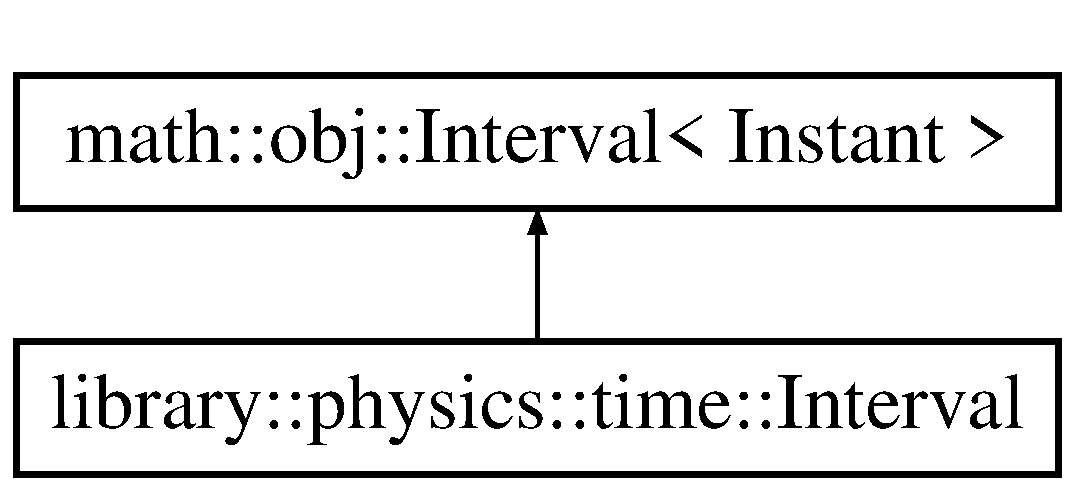
\includegraphics[height=2.000000cm]{classlibrary_1_1physics_1_1time_1_1_interval}
\end{center}
\end{figure}
\subsection*{Public Types}
\begin{DoxyCompactItemize}
\item 
typedef math\+::obj\+::\+Interval$<$ \hyperlink{classlibrary_1_1physics_1_1time_1_1_instant}{Instant} $>$\+::\hyperlink{classlibrary_1_1physics_1_1time_1_1_interval_aba490e7120a05be7b17a4d8076f25d48}{Type} \hyperlink{classlibrary_1_1physics_1_1time_1_1_interval_aba490e7120a05be7b17a4d8076f25d48}{Type}
\end{DoxyCompactItemize}
\subsection*{Public Member Functions}
\begin{DoxyCompactItemize}
\item 
\hyperlink{classlibrary_1_1physics_1_1time_1_1_interval_a49747b0d5f97a92d17f933a23b636156}{Interval} (const \hyperlink{classlibrary_1_1physics_1_1time_1_1_instant}{Instant} \&a\+Lower\+Bound, const \hyperlink{classlibrary_1_1physics_1_1time_1_1_instant}{Instant} \&an\+Upper\+Bound, const \hyperlink{classlibrary_1_1physics_1_1time_1_1_interval_aba490e7120a05be7b17a4d8076f25d48}{Interval\+::\+Type} \&an\+Interval\+Type)
\begin{DoxyCompactList}\small\item\em Constructor. \end{DoxyCompactList}\item 
bool \hyperlink{classlibrary_1_1physics_1_1time_1_1_interval_abbcbeb73fa6528c3e97d6e0c8b4592d8}{is\+Defined} () const
\item 
const \hyperlink{classlibrary_1_1physics_1_1time_1_1_instant}{Instant} \& \hyperlink{classlibrary_1_1physics_1_1time_1_1_interval_a954f0bc3e13e64956e697b4f87521c07}{access\+Start} () const
\item 
const \hyperlink{classlibrary_1_1physics_1_1time_1_1_instant}{Instant} \& \hyperlink{classlibrary_1_1physics_1_1time_1_1_interval_acdf92b0713da0d9691f5c25acb4c8001}{access\+End} () const
\item 
\hyperlink{classlibrary_1_1physics_1_1time_1_1_instant}{Instant} \hyperlink{classlibrary_1_1physics_1_1time_1_1_interval_a17fe30453121eac9666827f9e64e0a52}{get\+Start} () const
\item 
\hyperlink{classlibrary_1_1physics_1_1time_1_1_instant}{Instant} \hyperlink{classlibrary_1_1physics_1_1time_1_1_interval_ae61db32de1d59012b0fcea67d9c4f102}{get\+End} () const
\item 
\hyperlink{classlibrary_1_1physics_1_1time_1_1_duration}{Duration} \hyperlink{classlibrary_1_1physics_1_1time_1_1_interval_aab7bd7557fe401d9dd39716679a922af}{get\+Duration} () const
\item 
\hyperlink{classlibrary_1_1physics_1_1time_1_1_instant}{Instant} \hyperlink{classlibrary_1_1physics_1_1time_1_1_interval_aadbe0ae610cc0cd188d94c41b7a03ade}{get\+Center} () const
\item 
String \hyperlink{classlibrary_1_1physics_1_1time_1_1_interval_a1a76aed1663bc669e8115425e86f993e}{to\+String} (const \hyperlink{namespacelibrary_1_1physics_1_1time_a09d2bc9fbc7b0b5f92e1419bd655e6bb}{Scale} \&a\+Time\+Scale=\hyperlink{namespacelibrary_1_1physics_1_1time_a09d2bc9fbc7b0b5f92e1419bd655e6bba9234324ddf6b4176b57d803a925b7961}{Scale\+::\+U\+TC}) const
\item 
Array$<$ \hyperlink{classlibrary_1_1physics_1_1time_1_1_instant}{Instant} $>$ \hyperlink{classlibrary_1_1physics_1_1time_1_1_interval_aac7b4202a0d0079f59be089b6049beb3}{generate\+Grid} (const \hyperlink{classlibrary_1_1physics_1_1time_1_1_duration}{Duration} \&a\+Time\+Step) const
\end{DoxyCompactItemize}
\subsection*{Static Public Member Functions}
\begin{DoxyCompactItemize}
\item 
static \hyperlink{classlibrary_1_1physics_1_1time_1_1_interval}{Interval} \hyperlink{classlibrary_1_1physics_1_1time_1_1_interval_abe72d726e34919b4c8803e53af7fba66}{Undefined} ()
\item 
static \hyperlink{classlibrary_1_1physics_1_1time_1_1_interval}{Interval} \hyperlink{classlibrary_1_1physics_1_1time_1_1_interval_a89f1ca4a439fdc5224e60a441e757803}{Closed} (const \hyperlink{classlibrary_1_1physics_1_1time_1_1_instant}{Instant} \&a\+Lower\+Bound, const \hyperlink{classlibrary_1_1physics_1_1time_1_1_instant}{Instant} \&an\+Upper\+Bound)
\begin{DoxyCompactList}\small\item\em Constructs a closed interval. \end{DoxyCompactList}\item 
static \hyperlink{classlibrary_1_1physics_1_1time_1_1_interval}{Interval} \hyperlink{classlibrary_1_1physics_1_1time_1_1_interval_a052f385e80dea392c9ef5b52ed9443a1}{Centered} (const \hyperlink{classlibrary_1_1physics_1_1time_1_1_instant}{Instant} \&a\+Central\+Instant, const \hyperlink{classlibrary_1_1physics_1_1time_1_1_duration}{Duration} \&a\+Duration, const \hyperlink{classlibrary_1_1physics_1_1time_1_1_interval_aba490e7120a05be7b17a4d8076f25d48}{Interval\+::\+Type} \&an\+Interval\+Type)
\item 
static \hyperlink{classlibrary_1_1physics_1_1time_1_1_interval}{Interval} \hyperlink{classlibrary_1_1physics_1_1time_1_1_interval_a4f56de8af3b111650270abef273823bb}{Parse} (const String \&a\+String)
\begin{DoxyCompactList}\small\item\em Constructs an interval from a string representation. \end{DoxyCompactList}\end{DoxyCompactItemize}
\subsection*{Friends}
\begin{DoxyCompactItemize}
\item 
std\+::ostream \& \hyperlink{classlibrary_1_1physics_1_1time_1_1_interval_a4671ce6746f99155561a1bdfade9749a}{operator$<$$<$} (std\+::ostream \&an\+Output\+Stream, const \hyperlink{classlibrary_1_1physics_1_1time_1_1_interval}{Interval} \&an\+Interval)
\end{DoxyCompactItemize}


\subsection{Detailed Description}
\hyperlink{classlibrary_1_1physics_1_1time_1_1_interval}{Interval}. 

\subsection{Member Typedef Documentation}
\mbox{\Hypertarget{classlibrary_1_1physics_1_1time_1_1_interval_aba490e7120a05be7b17a4d8076f25d48}\label{classlibrary_1_1physics_1_1time_1_1_interval_aba490e7120a05be7b17a4d8076f25d48}} 
\index{library\+::physics\+::time\+::\+Interval@{library\+::physics\+::time\+::\+Interval}!Type@{Type}}
\index{Type@{Type}!library\+::physics\+::time\+::\+Interval@{library\+::physics\+::time\+::\+Interval}}
\subsubsection{\texorpdfstring{Type}{Type}}
{\footnotesize\ttfamily typedef math\+::obj\+::\+Interval$<$\hyperlink{classlibrary_1_1physics_1_1time_1_1_instant}{Instant}$>$\+::\hyperlink{classlibrary_1_1physics_1_1time_1_1_interval_aba490e7120a05be7b17a4d8076f25d48}{Type} \hyperlink{classlibrary_1_1physics_1_1time_1_1_interval_aba490e7120a05be7b17a4d8076f25d48}{library\+::physics\+::time\+::\+Interval\+::\+Type}}



\subsection{Constructor \& Destructor Documentation}
\mbox{\Hypertarget{classlibrary_1_1physics_1_1time_1_1_interval_a49747b0d5f97a92d17f933a23b636156}\label{classlibrary_1_1physics_1_1time_1_1_interval_a49747b0d5f97a92d17f933a23b636156}} 
\index{library\+::physics\+::time\+::\+Interval@{library\+::physics\+::time\+::\+Interval}!Interval@{Interval}}
\index{Interval@{Interval}!library\+::physics\+::time\+::\+Interval@{library\+::physics\+::time\+::\+Interval}}
\subsubsection{\texorpdfstring{Interval()}{Interval()}}
{\footnotesize\ttfamily library\+::physics\+::time\+::\+Interval\+::\+Interval (\begin{DoxyParamCaption}\item[{const \hyperlink{classlibrary_1_1physics_1_1time_1_1_instant}{Instant} \&}]{a\+Lower\+Bound,  }\item[{const \hyperlink{classlibrary_1_1physics_1_1time_1_1_instant}{Instant} \&}]{an\+Upper\+Bound,  }\item[{const \hyperlink{classlibrary_1_1physics_1_1time_1_1_interval_aba490e7120a05be7b17a4d8076f25d48}{Interval\+::\+Type} \&}]{an\+Interval\+Type }\end{DoxyParamCaption})}



Constructor. 


\begin{DoxyCode}
\hyperlink{classlibrary_1_1physics_1_1time_1_1_interval_a49747b0d5f97a92d17f933a23b636156}{Interval} interval(\hyperlink{classlibrary_1_1physics_1_1time_1_1_instant_a2a4f57aa71693b8def06788d55bc3bd3}{Instant::J2000}(), \hyperlink{classlibrary_1_1physics_1_1time_1_1_instant_abdee2ddacb34859a3be2a4cf97c4af81}{Instant::Now}(), 
      Interval::Type::Closed) ;
\end{DoxyCode}



\begin{DoxyParams}[1]{Parameters}
\mbox{\tt in}  & {\em a\+Lower\+Bound} & A lower bound \\
\hline
\mbox{\tt in}  & {\em an\+Upper\+Bound} & An upper bound \\
\hline
\mbox{\tt in}  & {\em an\+Interval\+Type} & An interval type \\
\hline
\end{DoxyParams}


\subsection{Member Function Documentation}
\mbox{\Hypertarget{classlibrary_1_1physics_1_1time_1_1_interval_acdf92b0713da0d9691f5c25acb4c8001}\label{classlibrary_1_1physics_1_1time_1_1_interval_acdf92b0713da0d9691f5c25acb4c8001}} 
\index{library\+::physics\+::time\+::\+Interval@{library\+::physics\+::time\+::\+Interval}!access\+End@{access\+End}}
\index{access\+End@{access\+End}!library\+::physics\+::time\+::\+Interval@{library\+::physics\+::time\+::\+Interval}}
\subsubsection{\texorpdfstring{access\+End()}{accessEnd()}}
{\footnotesize\ttfamily const \hyperlink{classlibrary_1_1physics_1_1time_1_1_instant}{Instant} \& library\+::physics\+::time\+::\+Interval\+::access\+End (\begin{DoxyParamCaption}{ }\end{DoxyParamCaption}) const}

\mbox{\Hypertarget{classlibrary_1_1physics_1_1time_1_1_interval_a954f0bc3e13e64956e697b4f87521c07}\label{classlibrary_1_1physics_1_1time_1_1_interval_a954f0bc3e13e64956e697b4f87521c07}} 
\index{library\+::physics\+::time\+::\+Interval@{library\+::physics\+::time\+::\+Interval}!access\+Start@{access\+Start}}
\index{access\+Start@{access\+Start}!library\+::physics\+::time\+::\+Interval@{library\+::physics\+::time\+::\+Interval}}
\subsubsection{\texorpdfstring{access\+Start()}{accessStart()}}
{\footnotesize\ttfamily const \hyperlink{classlibrary_1_1physics_1_1time_1_1_instant}{Instant} \& library\+::physics\+::time\+::\+Interval\+::access\+Start (\begin{DoxyParamCaption}{ }\end{DoxyParamCaption}) const}

\mbox{\Hypertarget{classlibrary_1_1physics_1_1time_1_1_interval_a052f385e80dea392c9ef5b52ed9443a1}\label{classlibrary_1_1physics_1_1time_1_1_interval_a052f385e80dea392c9ef5b52ed9443a1}} 
\index{library\+::physics\+::time\+::\+Interval@{library\+::physics\+::time\+::\+Interval}!Centered@{Centered}}
\index{Centered@{Centered}!library\+::physics\+::time\+::\+Interval@{library\+::physics\+::time\+::\+Interval}}
\subsubsection{\texorpdfstring{Centered()}{Centered()}}
{\footnotesize\ttfamily \hyperlink{classlibrary_1_1physics_1_1time_1_1_interval}{Interval} library\+::physics\+::time\+::\+Interval\+::\+Centered (\begin{DoxyParamCaption}\item[{const \hyperlink{classlibrary_1_1physics_1_1time_1_1_instant}{Instant} \&}]{a\+Central\+Instant,  }\item[{const \hyperlink{classlibrary_1_1physics_1_1time_1_1_duration}{Duration} \&}]{a\+Duration,  }\item[{const \hyperlink{classlibrary_1_1physics_1_1time_1_1_interval_aba490e7120a05be7b17a4d8076f25d48}{Interval\+::\+Type} \&}]{an\+Interval\+Type }\end{DoxyParamCaption})\hspace{0.3cm}{\ttfamily [static]}}

\mbox{\Hypertarget{classlibrary_1_1physics_1_1time_1_1_interval_a89f1ca4a439fdc5224e60a441e757803}\label{classlibrary_1_1physics_1_1time_1_1_interval_a89f1ca4a439fdc5224e60a441e757803}} 
\index{library\+::physics\+::time\+::\+Interval@{library\+::physics\+::time\+::\+Interval}!Closed@{Closed}}
\index{Closed@{Closed}!library\+::physics\+::time\+::\+Interval@{library\+::physics\+::time\+::\+Interval}}
\subsubsection{\texorpdfstring{Closed()}{Closed()}}
{\footnotesize\ttfamily \hyperlink{classlibrary_1_1physics_1_1time_1_1_interval}{Interval} library\+::physics\+::time\+::\+Interval\+::\+Closed (\begin{DoxyParamCaption}\item[{const \hyperlink{classlibrary_1_1physics_1_1time_1_1_instant}{Instant} \&}]{a\+Lower\+Bound,  }\item[{const \hyperlink{classlibrary_1_1physics_1_1time_1_1_instant}{Instant} \&}]{an\+Upper\+Bound }\end{DoxyParamCaption})\hspace{0.3cm}{\ttfamily [static]}}



Constructs a closed interval. 


\begin{DoxyCode}
\hyperlink{classlibrary_1_1physics_1_1time_1_1_interval_a49747b0d5f97a92d17f933a23b636156}{Interval} interval = \hyperlink{classlibrary_1_1physics_1_1time_1_1_interval_a89f1ca4a439fdc5224e60a441e757803}{Interval::Closed}(\hyperlink{classlibrary_1_1physics_1_1time_1_1_instant_a2a4f57aa71693b8def06788d55bc3bd3}{Instant::J2000}(), 
      \hyperlink{classlibrary_1_1physics_1_1time_1_1_instant_abdee2ddacb34859a3be2a4cf97c4af81}{Instant::Now}()) ; \textcolor{comment}{// [J2000, Now]}
\end{DoxyCode}


\begin{DoxyReturn}{Returns}
Closed interval 
\end{DoxyReturn}
\mbox{\Hypertarget{classlibrary_1_1physics_1_1time_1_1_interval_aac7b4202a0d0079f59be089b6049beb3}\label{classlibrary_1_1physics_1_1time_1_1_interval_aac7b4202a0d0079f59be089b6049beb3}} 
\index{library\+::physics\+::time\+::\+Interval@{library\+::physics\+::time\+::\+Interval}!generate\+Grid@{generate\+Grid}}
\index{generate\+Grid@{generate\+Grid}!library\+::physics\+::time\+::\+Interval@{library\+::physics\+::time\+::\+Interval}}
\subsubsection{\texorpdfstring{generate\+Grid()}{generateGrid()}}
{\footnotesize\ttfamily Array$<$ \hyperlink{classlibrary_1_1physics_1_1time_1_1_instant}{Instant} $>$ library\+::physics\+::time\+::\+Interval\+::generate\+Grid (\begin{DoxyParamCaption}\item[{const \hyperlink{classlibrary_1_1physics_1_1time_1_1_duration}{Duration} \&}]{a\+Time\+Step }\end{DoxyParamCaption}) const}

\mbox{\Hypertarget{classlibrary_1_1physics_1_1time_1_1_interval_aadbe0ae610cc0cd188d94c41b7a03ade}\label{classlibrary_1_1physics_1_1time_1_1_interval_aadbe0ae610cc0cd188d94c41b7a03ade}} 
\index{library\+::physics\+::time\+::\+Interval@{library\+::physics\+::time\+::\+Interval}!get\+Center@{get\+Center}}
\index{get\+Center@{get\+Center}!library\+::physics\+::time\+::\+Interval@{library\+::physics\+::time\+::\+Interval}}
\subsubsection{\texorpdfstring{get\+Center()}{getCenter()}}
{\footnotesize\ttfamily \hyperlink{classlibrary_1_1physics_1_1time_1_1_instant}{Instant} library\+::physics\+::time\+::\+Interval\+::get\+Center (\begin{DoxyParamCaption}{ }\end{DoxyParamCaption}) const}

\mbox{\Hypertarget{classlibrary_1_1physics_1_1time_1_1_interval_aab7bd7557fe401d9dd39716679a922af}\label{classlibrary_1_1physics_1_1time_1_1_interval_aab7bd7557fe401d9dd39716679a922af}} 
\index{library\+::physics\+::time\+::\+Interval@{library\+::physics\+::time\+::\+Interval}!get\+Duration@{get\+Duration}}
\index{get\+Duration@{get\+Duration}!library\+::physics\+::time\+::\+Interval@{library\+::physics\+::time\+::\+Interval}}
\subsubsection{\texorpdfstring{get\+Duration()}{getDuration()}}
{\footnotesize\ttfamily \hyperlink{classlibrary_1_1physics_1_1time_1_1_duration}{Duration} library\+::physics\+::time\+::\+Interval\+::get\+Duration (\begin{DoxyParamCaption}{ }\end{DoxyParamCaption}) const}

\mbox{\Hypertarget{classlibrary_1_1physics_1_1time_1_1_interval_ae61db32de1d59012b0fcea67d9c4f102}\label{classlibrary_1_1physics_1_1time_1_1_interval_ae61db32de1d59012b0fcea67d9c4f102}} 
\index{library\+::physics\+::time\+::\+Interval@{library\+::physics\+::time\+::\+Interval}!get\+End@{get\+End}}
\index{get\+End@{get\+End}!library\+::physics\+::time\+::\+Interval@{library\+::physics\+::time\+::\+Interval}}
\subsubsection{\texorpdfstring{get\+End()}{getEnd()}}
{\footnotesize\ttfamily \hyperlink{classlibrary_1_1physics_1_1time_1_1_instant}{Instant} library\+::physics\+::time\+::\+Interval\+::get\+End (\begin{DoxyParamCaption}{ }\end{DoxyParamCaption}) const}

\mbox{\Hypertarget{classlibrary_1_1physics_1_1time_1_1_interval_a17fe30453121eac9666827f9e64e0a52}\label{classlibrary_1_1physics_1_1time_1_1_interval_a17fe30453121eac9666827f9e64e0a52}} 
\index{library\+::physics\+::time\+::\+Interval@{library\+::physics\+::time\+::\+Interval}!get\+Start@{get\+Start}}
\index{get\+Start@{get\+Start}!library\+::physics\+::time\+::\+Interval@{library\+::physics\+::time\+::\+Interval}}
\subsubsection{\texorpdfstring{get\+Start()}{getStart()}}
{\footnotesize\ttfamily \hyperlink{classlibrary_1_1physics_1_1time_1_1_instant}{Instant} library\+::physics\+::time\+::\+Interval\+::get\+Start (\begin{DoxyParamCaption}{ }\end{DoxyParamCaption}) const}

\mbox{\Hypertarget{classlibrary_1_1physics_1_1time_1_1_interval_abbcbeb73fa6528c3e97d6e0c8b4592d8}\label{classlibrary_1_1physics_1_1time_1_1_interval_abbcbeb73fa6528c3e97d6e0c8b4592d8}} 
\index{library\+::physics\+::time\+::\+Interval@{library\+::physics\+::time\+::\+Interval}!is\+Defined@{is\+Defined}}
\index{is\+Defined@{is\+Defined}!library\+::physics\+::time\+::\+Interval@{library\+::physics\+::time\+::\+Interval}}
\subsubsection{\texorpdfstring{is\+Defined()}{isDefined()}}
{\footnotesize\ttfamily bool library\+::physics\+::time\+::\+Interval\+::is\+Defined (\begin{DoxyParamCaption}{ }\end{DoxyParamCaption}) const}

\mbox{\Hypertarget{classlibrary_1_1physics_1_1time_1_1_interval_a4f56de8af3b111650270abef273823bb}\label{classlibrary_1_1physics_1_1time_1_1_interval_a4f56de8af3b111650270abef273823bb}} 
\index{library\+::physics\+::time\+::\+Interval@{library\+::physics\+::time\+::\+Interval}!Parse@{Parse}}
\index{Parse@{Parse}!library\+::physics\+::time\+::\+Interval@{library\+::physics\+::time\+::\+Interval}}
\subsubsection{\texorpdfstring{Parse()}{Parse()}}
{\footnotesize\ttfamily \hyperlink{classlibrary_1_1physics_1_1time_1_1_interval}{Interval} library\+::physics\+::time\+::\+Interval\+::\+Parse (\begin{DoxyParamCaption}\item[{const String \&}]{a\+String }\end{DoxyParamCaption})\hspace{0.3cm}{\ttfamily [static]}}



Constructs an interval from a string representation. 


\begin{DoxyCode}
...
\end{DoxyCode}



\begin{DoxyParams}[1]{Parameters}
\mbox{\tt in}  & {\em a\+String} & A string \\
\hline
\end{DoxyParams}
\begin{DoxyReturn}{Returns}
\hyperlink{classlibrary_1_1physics_1_1time_1_1_interval}{Interval} 
\end{DoxyReturn}
\mbox{\Hypertarget{classlibrary_1_1physics_1_1time_1_1_interval_a1a76aed1663bc669e8115425e86f993e}\label{classlibrary_1_1physics_1_1time_1_1_interval_a1a76aed1663bc669e8115425e86f993e}} 
\index{library\+::physics\+::time\+::\+Interval@{library\+::physics\+::time\+::\+Interval}!to\+String@{to\+String}}
\index{to\+String@{to\+String}!library\+::physics\+::time\+::\+Interval@{library\+::physics\+::time\+::\+Interval}}
\subsubsection{\texorpdfstring{to\+String()}{toString()}}
{\footnotesize\ttfamily String library\+::physics\+::time\+::\+Interval\+::to\+String (\begin{DoxyParamCaption}\item[{const \hyperlink{namespacelibrary_1_1physics_1_1time_a09d2bc9fbc7b0b5f92e1419bd655e6bb}{Scale} \&}]{a\+Time\+Scale = {\ttfamily \hyperlink{namespacelibrary_1_1physics_1_1time_a09d2bc9fbc7b0b5f92e1419bd655e6bba9234324ddf6b4176b57d803a925b7961}{Scale\+::\+U\+TC}} }\end{DoxyParamCaption}) const}

\mbox{\Hypertarget{classlibrary_1_1physics_1_1time_1_1_interval_abe72d726e34919b4c8803e53af7fba66}\label{classlibrary_1_1physics_1_1time_1_1_interval_abe72d726e34919b4c8803e53af7fba66}} 
\index{library\+::physics\+::time\+::\+Interval@{library\+::physics\+::time\+::\+Interval}!Undefined@{Undefined}}
\index{Undefined@{Undefined}!library\+::physics\+::time\+::\+Interval@{library\+::physics\+::time\+::\+Interval}}
\subsubsection{\texorpdfstring{Undefined()}{Undefined()}}
{\footnotesize\ttfamily \hyperlink{classlibrary_1_1physics_1_1time_1_1_interval}{Interval} library\+::physics\+::time\+::\+Interval\+::\+Undefined (\begin{DoxyParamCaption}{ }\end{DoxyParamCaption})\hspace{0.3cm}{\ttfamily [static]}}



\subsection{Friends And Related Function Documentation}
\mbox{\Hypertarget{classlibrary_1_1physics_1_1time_1_1_interval_a4671ce6746f99155561a1bdfade9749a}\label{classlibrary_1_1physics_1_1time_1_1_interval_a4671ce6746f99155561a1bdfade9749a}} 
\index{library\+::physics\+::time\+::\+Interval@{library\+::physics\+::time\+::\+Interval}!operator$<$$<$@{operator$<$$<$}}
\index{operator$<$$<$@{operator$<$$<$}!library\+::physics\+::time\+::\+Interval@{library\+::physics\+::time\+::\+Interval}}
\subsubsection{\texorpdfstring{operator$<$$<$}{operator<<}}
{\footnotesize\ttfamily std\+::ostream\& operator$<$$<$ (\begin{DoxyParamCaption}\item[{std\+::ostream \&}]{an\+Output\+Stream,  }\item[{const \hyperlink{classlibrary_1_1physics_1_1time_1_1_interval}{Interval} \&}]{an\+Interval }\end{DoxyParamCaption})\hspace{0.3cm}{\ttfamily [friend]}}



The documentation for this class was generated from the following files\+:\begin{DoxyCompactItemize}
\item 
include/\+Library/\+Physics/\+Time/\hyperlink{_interval_8hpp}{Interval.\+hpp}\item 
src/\+Library/\+Physics/\+Time/\hyperlink{_interval_8cpp}{Interval.\+cpp}\end{DoxyCompactItemize}

\hypertarget{classlibrary_1_1physics_1_1coord_1_1frame_1_1provider_1_1_i_t_r_f}{}\section{library\+:\+:physics\+:\+:coord\+:\+:frame\+:\+:provider\+:\+:I\+T\+RF Class Reference}
\label{classlibrary_1_1physics_1_1coord_1_1frame_1_1provider_1_1_i_t_r_f}\index{library\+::physics\+::coord\+::frame\+::provider\+::\+I\+T\+RF@{library\+::physics\+::coord\+::frame\+::provider\+::\+I\+T\+RF}}


International Terrestrial Reference System (\hyperlink{classlibrary_1_1physics_1_1coord_1_1frame_1_1provider_1_1_i_t_r_f}{I\+T\+RF}) provider.  




{\ttfamily \#include $<$I\+T\+R\+F.\+hpp$>$}

Inheritance diagram for library\+:\+:physics\+:\+:coord\+:\+:frame\+:\+:provider\+:\+:I\+T\+RF\+:\begin{figure}[H]
\begin{center}
\leavevmode
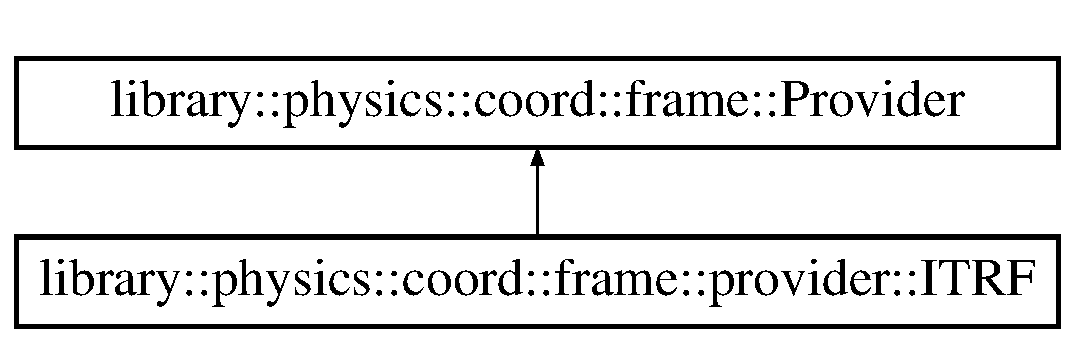
\includegraphics[height=2.000000cm]{classlibrary_1_1physics_1_1coord_1_1frame_1_1provider_1_1_i_t_r_f}
\end{center}
\end{figure}
\subsection*{Public Member Functions}
\begin{DoxyCompactItemize}
\item 
\hyperlink{classlibrary_1_1physics_1_1coord_1_1frame_1_1provider_1_1_i_t_r_f_a9c90e2865d4f076866d6d6d58e7f2e37}{I\+T\+RF} ()
\item 
virtual \hyperlink{classlibrary_1_1physics_1_1coord_1_1frame_1_1provider_1_1_i_t_r_f_a2b6d9949dcfcd4cbff44a92b8c137e9c}{$\sim$\+I\+T\+RF} () override
\item 
virtual \hyperlink{classlibrary_1_1physics_1_1coord_1_1frame_1_1provider_1_1_i_t_r_f}{I\+T\+RF} $\ast$ \hyperlink{classlibrary_1_1physics_1_1coord_1_1frame_1_1provider_1_1_i_t_r_f_a0408f17419e49f785863ba7a84865857}{clone} () const override
\item 
virtual bool \hyperlink{classlibrary_1_1physics_1_1coord_1_1frame_1_1provider_1_1_i_t_r_f_a10a6a129ab5410f3ad3d687f73ba6d8e}{is\+Defined} () const override
\item 
virtual \hyperlink{classlibrary_1_1physics_1_1coord_1_1_transform}{Transform} \hyperlink{classlibrary_1_1physics_1_1coord_1_1frame_1_1provider_1_1_i_t_r_f_a9fcd6914fa436788b84923a45fe1014e}{get\+Transform\+At} (const \hyperlink{classlibrary_1_1physics_1_1time_1_1_instant}{Instant} \&an\+Instant) const override
\end{DoxyCompactItemize}


\subsection{Detailed Description}
International Terrestrial Reference System (\hyperlink{classlibrary_1_1physics_1_1coord_1_1frame_1_1provider_1_1_i_t_r_f}{I\+T\+RF}) provider. 

https\+://en.wikipedia.\+org/wiki/\+International\+\_\+\+Terrestrial\+\_\+\+Reference\+\_\+\+System 

\subsection{Constructor \& Destructor Documentation}
\mbox{\Hypertarget{classlibrary_1_1physics_1_1coord_1_1frame_1_1provider_1_1_i_t_r_f_a9c90e2865d4f076866d6d6d58e7f2e37}\label{classlibrary_1_1physics_1_1coord_1_1frame_1_1provider_1_1_i_t_r_f_a9c90e2865d4f076866d6d6d58e7f2e37}} 
\index{library\+::physics\+::coord\+::frame\+::provider\+::\+I\+T\+RF@{library\+::physics\+::coord\+::frame\+::provider\+::\+I\+T\+RF}!I\+T\+RF@{I\+T\+RF}}
\index{I\+T\+RF@{I\+T\+RF}!library\+::physics\+::coord\+::frame\+::provider\+::\+I\+T\+RF@{library\+::physics\+::coord\+::frame\+::provider\+::\+I\+T\+RF}}
\subsubsection{\texorpdfstring{I\+T\+R\+F()}{ITRF()}}
{\footnotesize\ttfamily library\+::physics\+::coord\+::frame\+::provider\+::\+I\+T\+R\+F\+::\+I\+T\+RF (\begin{DoxyParamCaption}{ }\end{DoxyParamCaption})}

\mbox{\Hypertarget{classlibrary_1_1physics_1_1coord_1_1frame_1_1provider_1_1_i_t_r_f_a2b6d9949dcfcd4cbff44a92b8c137e9c}\label{classlibrary_1_1physics_1_1coord_1_1frame_1_1provider_1_1_i_t_r_f_a2b6d9949dcfcd4cbff44a92b8c137e9c}} 
\index{library\+::physics\+::coord\+::frame\+::provider\+::\+I\+T\+RF@{library\+::physics\+::coord\+::frame\+::provider\+::\+I\+T\+RF}!````~I\+T\+RF@{$\sim$\+I\+T\+RF}}
\index{````~I\+T\+RF@{$\sim$\+I\+T\+RF}!library\+::physics\+::coord\+::frame\+::provider\+::\+I\+T\+RF@{library\+::physics\+::coord\+::frame\+::provider\+::\+I\+T\+RF}}
\subsubsection{\texorpdfstring{$\sim$\+I\+T\+R\+F()}{~ITRF()}}
{\footnotesize\ttfamily library\+::physics\+::coord\+::frame\+::provider\+::\+I\+T\+R\+F\+::$\sim$\+I\+T\+RF (\begin{DoxyParamCaption}{ }\end{DoxyParamCaption})\hspace{0.3cm}{\ttfamily [override]}, {\ttfamily [virtual]}}



\subsection{Member Function Documentation}
\mbox{\Hypertarget{classlibrary_1_1physics_1_1coord_1_1frame_1_1provider_1_1_i_t_r_f_a0408f17419e49f785863ba7a84865857}\label{classlibrary_1_1physics_1_1coord_1_1frame_1_1provider_1_1_i_t_r_f_a0408f17419e49f785863ba7a84865857}} 
\index{library\+::physics\+::coord\+::frame\+::provider\+::\+I\+T\+RF@{library\+::physics\+::coord\+::frame\+::provider\+::\+I\+T\+RF}!clone@{clone}}
\index{clone@{clone}!library\+::physics\+::coord\+::frame\+::provider\+::\+I\+T\+RF@{library\+::physics\+::coord\+::frame\+::provider\+::\+I\+T\+RF}}
\subsubsection{\texorpdfstring{clone()}{clone()}}
{\footnotesize\ttfamily \hyperlink{classlibrary_1_1physics_1_1coord_1_1frame_1_1provider_1_1_i_t_r_f}{I\+T\+RF} $\ast$ library\+::physics\+::coord\+::frame\+::provider\+::\+I\+T\+R\+F\+::clone (\begin{DoxyParamCaption}{ }\end{DoxyParamCaption}) const\hspace{0.3cm}{\ttfamily [override]}, {\ttfamily [virtual]}}



Implements \hyperlink{classlibrary_1_1physics_1_1coord_1_1frame_1_1_provider_ab8eee40c8ef4aee0b57bedf458f4934e}{library\+::physics\+::coord\+::frame\+::\+Provider}.

\mbox{\Hypertarget{classlibrary_1_1physics_1_1coord_1_1frame_1_1provider_1_1_i_t_r_f_a9fcd6914fa436788b84923a45fe1014e}\label{classlibrary_1_1physics_1_1coord_1_1frame_1_1provider_1_1_i_t_r_f_a9fcd6914fa436788b84923a45fe1014e}} 
\index{library\+::physics\+::coord\+::frame\+::provider\+::\+I\+T\+RF@{library\+::physics\+::coord\+::frame\+::provider\+::\+I\+T\+RF}!get\+Transform\+At@{get\+Transform\+At}}
\index{get\+Transform\+At@{get\+Transform\+At}!library\+::physics\+::coord\+::frame\+::provider\+::\+I\+T\+RF@{library\+::physics\+::coord\+::frame\+::provider\+::\+I\+T\+RF}}
\subsubsection{\texorpdfstring{get\+Transform\+At()}{getTransformAt()}}
{\footnotesize\ttfamily \hyperlink{classlibrary_1_1physics_1_1coord_1_1_transform}{Transform} library\+::physics\+::coord\+::frame\+::provider\+::\+I\+T\+R\+F\+::get\+Transform\+At (\begin{DoxyParamCaption}\item[{const \hyperlink{classlibrary_1_1physics_1_1time_1_1_instant}{Instant} \&}]{an\+Instant }\end{DoxyParamCaption}) const\hspace{0.3cm}{\ttfamily [override]}, {\ttfamily [virtual]}}



Implements \hyperlink{classlibrary_1_1physics_1_1coord_1_1frame_1_1_provider_a796fd2dd337f1304a0e9acf573ce2550}{library\+::physics\+::coord\+::frame\+::\+Provider}.

\mbox{\Hypertarget{classlibrary_1_1physics_1_1coord_1_1frame_1_1provider_1_1_i_t_r_f_a10a6a129ab5410f3ad3d687f73ba6d8e}\label{classlibrary_1_1physics_1_1coord_1_1frame_1_1provider_1_1_i_t_r_f_a10a6a129ab5410f3ad3d687f73ba6d8e}} 
\index{library\+::physics\+::coord\+::frame\+::provider\+::\+I\+T\+RF@{library\+::physics\+::coord\+::frame\+::provider\+::\+I\+T\+RF}!is\+Defined@{is\+Defined}}
\index{is\+Defined@{is\+Defined}!library\+::physics\+::coord\+::frame\+::provider\+::\+I\+T\+RF@{library\+::physics\+::coord\+::frame\+::provider\+::\+I\+T\+RF}}
\subsubsection{\texorpdfstring{is\+Defined()}{isDefined()}}
{\footnotesize\ttfamily bool library\+::physics\+::coord\+::frame\+::provider\+::\+I\+T\+R\+F\+::is\+Defined (\begin{DoxyParamCaption}{ }\end{DoxyParamCaption}) const\hspace{0.3cm}{\ttfamily [override]}, {\ttfamily [virtual]}}



Implements \hyperlink{classlibrary_1_1physics_1_1coord_1_1frame_1_1_provider_ae7cd093febf2b20f71400f9f79442774}{library\+::physics\+::coord\+::frame\+::\+Provider}.



The documentation for this class was generated from the following files\+:\begin{DoxyCompactItemize}
\item 
include/\+Library/\+Physics/\+Coordinate/\+Frame/\+Providers/\hyperlink{_i_t_r_f_8hpp}{I\+T\+R\+F.\+hpp}\item 
src/\+Library/\+Physics/\+Coordinate/\+Frame/\+Providers/\hyperlink{_i_t_r_f_8cpp}{I\+T\+R\+F.\+cpp}\end{DoxyCompactItemize}

\hypertarget{classlibrary_1_1physics_1_1units_1_1_length}{}\section{library\+:\+:physics\+:\+:units\+:\+:Length Class Reference}
\label{classlibrary_1_1physics_1_1units_1_1_length}\index{library\+::physics\+::units\+::\+Length@{library\+::physics\+::units\+::\+Length}}


{\ttfamily \#include $<$Length.\+hpp$>$}

\subsection*{Public Member Functions}
\begin{DoxyCompactItemize}
\item 
\hyperlink{classlibrary_1_1physics_1_1units_1_1_length_abc75d349b771abc33d0e1a8bbac73a53}{Length} ()
\end{DoxyCompactItemize}


\subsection{Constructor \& Destructor Documentation}
\mbox{\Hypertarget{classlibrary_1_1physics_1_1units_1_1_length_abc75d349b771abc33d0e1a8bbac73a53}\label{classlibrary_1_1physics_1_1units_1_1_length_abc75d349b771abc33d0e1a8bbac73a53}} 
\index{library\+::physics\+::units\+::\+Length@{library\+::physics\+::units\+::\+Length}!Length@{Length}}
\index{Length@{Length}!library\+::physics\+::units\+::\+Length@{library\+::physics\+::units\+::\+Length}}
\subsubsection{\texorpdfstring{Length()}{Length()}}
{\footnotesize\ttfamily library\+::physics\+::units\+::\+Length\+::\+Length (\begin{DoxyParamCaption}{ }\end{DoxyParamCaption})}



The documentation for this class was generated from the following files\+:\begin{DoxyCompactItemize}
\item 
include/\+Library/\+Physics/\+Units/\hyperlink{_length_8hpp}{Length.\+hpp}\item 
src/\+Library/\+Physics/\+Units/\hyperlink{_length_8cpp}{Length.\+cpp}\end{DoxyCompactItemize}

\hypertarget{classlibrary_1_1physics_1_1coord_1_1spherical_1_1_l_l_a}{}\section{library\+:\+:physics\+:\+:coord\+:\+:spherical\+:\+:L\+LA Class Reference}
\label{classlibrary_1_1physics_1_1coord_1_1spherical_1_1_l_l_a}\index{library\+::physics\+::coord\+::spherical\+::\+L\+LA@{library\+::physics\+::coord\+::spherical\+::\+L\+LA}}


Geodetic Latitude -\/ Longitude -\/ Altitude (\hyperlink{classlibrary_1_1physics_1_1coord_1_1spherical_1_1_l_l_a}{L\+LA})  




{\ttfamily \#include $<$L\+L\+A.\+hpp$>$}

\subsection*{Public Member Functions}
\begin{DoxyCompactItemize}
\item 
\hyperlink{classlibrary_1_1physics_1_1coord_1_1spherical_1_1_l_l_a_af18b9011d2df6c1120e0f770ab1eb909}{L\+LA} (const \hyperlink{classlibrary_1_1physics_1_1units_1_1_angle}{Angle} \&a\+Latitude, const \hyperlink{classlibrary_1_1physics_1_1units_1_1_angle}{Angle} \&a\+Longitude, const \hyperlink{classlibrary_1_1physics_1_1units_1_1_length}{Length} \&an\+Altitude)
\item 
bool \hyperlink{classlibrary_1_1physics_1_1coord_1_1spherical_1_1_l_l_a_a104c505db9941b6d21c10e0478cdc1f2}{operator==} (const \hyperlink{classlibrary_1_1physics_1_1coord_1_1spherical_1_1_l_l_a}{L\+LA} \&a\+L\+LA) const
\item 
bool \hyperlink{classlibrary_1_1physics_1_1coord_1_1spherical_1_1_l_l_a_a150b8dd334c6874643a4675f9f67538b}{operator!=} (const \hyperlink{classlibrary_1_1physics_1_1coord_1_1spherical_1_1_l_l_a}{L\+LA} \&a\+L\+LA) const
\item 
bool \hyperlink{classlibrary_1_1physics_1_1coord_1_1spherical_1_1_l_l_a_a9784847b6e35cf506896e6810ec73f23}{is\+Defined} () const
\item 
\hyperlink{classlibrary_1_1physics_1_1units_1_1_angle}{Angle} \hyperlink{classlibrary_1_1physics_1_1coord_1_1spherical_1_1_l_l_a_a4cae48d00f1f5319c1560f1bfe1b2cb5}{get\+Latitude} () const
\item 
\hyperlink{classlibrary_1_1physics_1_1units_1_1_angle}{Angle} \hyperlink{classlibrary_1_1physics_1_1coord_1_1spherical_1_1_l_l_a_a55ca45ade10658e903628afb5e35fc56}{get\+Longitude} () const
\item 
\hyperlink{classlibrary_1_1physics_1_1units_1_1_length}{Length} \hyperlink{classlibrary_1_1physics_1_1coord_1_1spherical_1_1_l_l_a_a2f35237c136581669e9a49e310633b58}{get\+Altitude} () const
\item 
Vector3d \hyperlink{classlibrary_1_1physics_1_1coord_1_1spherical_1_1_l_l_a_aed6303008da6b6c85c3abdda2bd63c24}{to\+Vector} () const
\item 
Vector3d \hyperlink{classlibrary_1_1physics_1_1coord_1_1spherical_1_1_l_l_a_a345c00ef99eeb403a79453c7829b413c}{to\+Cartesian} (const \hyperlink{classlibrary_1_1physics_1_1units_1_1_length}{Length} \&an\+Ellipsoid\+Equatorial\+Radius, const Real \&an\+Ellipsoid\+Flattening) const
\item 
String \hyperlink{classlibrary_1_1physics_1_1coord_1_1spherical_1_1_l_l_a_a082872655279f13c9b524467064cb4bb}{to\+String} () const
\end{DoxyCompactItemize}
\subsection*{Static Public Member Functions}
\begin{DoxyCompactItemize}
\item 
static \hyperlink{classlibrary_1_1physics_1_1coord_1_1spherical_1_1_l_l_a}{L\+LA} \hyperlink{classlibrary_1_1physics_1_1coord_1_1spherical_1_1_l_l_a_a5e95fa01c321b58df585f510bfa27eea}{Undefined} ()
\item 
static \hyperlink{classlibrary_1_1physics_1_1coord_1_1spherical_1_1_l_l_a}{L\+LA} \hyperlink{classlibrary_1_1physics_1_1coord_1_1spherical_1_1_l_l_a_af20391360cdab4dbd94afb3d4ddeddbc}{Vector} (const Vector3d \&a\+Vector)
\item 
static \hyperlink{classlibrary_1_1physics_1_1coord_1_1spherical_1_1_l_l_a}{L\+LA} \hyperlink{classlibrary_1_1physics_1_1coord_1_1spherical_1_1_l_l_a_af48c6fa8a250c20befa8452d234537d1}{Cartesian} (const Vector3d \&a\+Cartesian\+Coordinate\+Set, const \hyperlink{classlibrary_1_1physics_1_1units_1_1_length}{Length} \&an\+Ellipsoid\+Equatorial\+Radius, const Real \&an\+Ellipsoid\+Flattening)
\end{DoxyCompactItemize}
\subsection*{Friends}
\begin{DoxyCompactItemize}
\item 
std\+::ostream \& \hyperlink{classlibrary_1_1physics_1_1coord_1_1spherical_1_1_l_l_a_a4e052cf41d11b11c943ad32cd4c25ba8}{operator$<$$<$} (std\+::ostream \&an\+Output\+Stream, const \hyperlink{classlibrary_1_1physics_1_1coord_1_1spherical_1_1_l_l_a}{L\+LA} \&a\+L\+LA)
\end{DoxyCompactItemize}


\subsection{Detailed Description}
Geodetic Latitude -\/ Longitude -\/ Altitude (\hyperlink{classlibrary_1_1physics_1_1coord_1_1spherical_1_1_l_l_a}{L\+LA}) 

https\+://en.wikipedia.\+org/wiki/\+Latitude https\+://en.wikipedia.\+org/wiki/\+Longitude 

\subsection{Constructor \& Destructor Documentation}
\mbox{\Hypertarget{classlibrary_1_1physics_1_1coord_1_1spherical_1_1_l_l_a_af18b9011d2df6c1120e0f770ab1eb909}\label{classlibrary_1_1physics_1_1coord_1_1spherical_1_1_l_l_a_af18b9011d2df6c1120e0f770ab1eb909}} 
\index{library\+::physics\+::coord\+::spherical\+::\+L\+LA@{library\+::physics\+::coord\+::spherical\+::\+L\+LA}!L\+LA@{L\+LA}}
\index{L\+LA@{L\+LA}!library\+::physics\+::coord\+::spherical\+::\+L\+LA@{library\+::physics\+::coord\+::spherical\+::\+L\+LA}}
\subsubsection{\texorpdfstring{L\+L\+A()}{LLA()}}
{\footnotesize\ttfamily library\+::physics\+::coord\+::spherical\+::\+L\+L\+A\+::\+L\+LA (\begin{DoxyParamCaption}\item[{const \hyperlink{classlibrary_1_1physics_1_1units_1_1_angle}{Angle} \&}]{a\+Latitude,  }\item[{const \hyperlink{classlibrary_1_1physics_1_1units_1_1_angle}{Angle} \&}]{a\+Longitude,  }\item[{const \hyperlink{classlibrary_1_1physics_1_1units_1_1_length}{Length} \&}]{an\+Altitude }\end{DoxyParamCaption})}



\subsection{Member Function Documentation}
\mbox{\Hypertarget{classlibrary_1_1physics_1_1coord_1_1spherical_1_1_l_l_a_af48c6fa8a250c20befa8452d234537d1}\label{classlibrary_1_1physics_1_1coord_1_1spherical_1_1_l_l_a_af48c6fa8a250c20befa8452d234537d1}} 
\index{library\+::physics\+::coord\+::spherical\+::\+L\+LA@{library\+::physics\+::coord\+::spherical\+::\+L\+LA}!Cartesian@{Cartesian}}
\index{Cartesian@{Cartesian}!library\+::physics\+::coord\+::spherical\+::\+L\+LA@{library\+::physics\+::coord\+::spherical\+::\+L\+LA}}
\subsubsection{\texorpdfstring{Cartesian()}{Cartesian()}}
{\footnotesize\ttfamily \hyperlink{classlibrary_1_1physics_1_1coord_1_1spherical_1_1_l_l_a}{L\+LA} library\+::physics\+::coord\+::spherical\+::\+L\+L\+A\+::\+Cartesian (\begin{DoxyParamCaption}\item[{const Vector3d \&}]{a\+Cartesian\+Coordinate\+Set,  }\item[{const \hyperlink{classlibrary_1_1physics_1_1units_1_1_length}{Length} \&}]{an\+Ellipsoid\+Equatorial\+Radius,  }\item[{const Real \&}]{an\+Ellipsoid\+Flattening }\end{DoxyParamCaption})\hspace{0.3cm}{\ttfamily [static]}}

\mbox{\Hypertarget{classlibrary_1_1physics_1_1coord_1_1spherical_1_1_l_l_a_a2f35237c136581669e9a49e310633b58}\label{classlibrary_1_1physics_1_1coord_1_1spherical_1_1_l_l_a_a2f35237c136581669e9a49e310633b58}} 
\index{library\+::physics\+::coord\+::spherical\+::\+L\+LA@{library\+::physics\+::coord\+::spherical\+::\+L\+LA}!get\+Altitude@{get\+Altitude}}
\index{get\+Altitude@{get\+Altitude}!library\+::physics\+::coord\+::spherical\+::\+L\+LA@{library\+::physics\+::coord\+::spherical\+::\+L\+LA}}
\subsubsection{\texorpdfstring{get\+Altitude()}{getAltitude()}}
{\footnotesize\ttfamily \hyperlink{classlibrary_1_1physics_1_1units_1_1_length}{Length} library\+::physics\+::coord\+::spherical\+::\+L\+L\+A\+::get\+Altitude (\begin{DoxyParamCaption}{ }\end{DoxyParamCaption}) const}

\mbox{\Hypertarget{classlibrary_1_1physics_1_1coord_1_1spherical_1_1_l_l_a_a4cae48d00f1f5319c1560f1bfe1b2cb5}\label{classlibrary_1_1physics_1_1coord_1_1spherical_1_1_l_l_a_a4cae48d00f1f5319c1560f1bfe1b2cb5}} 
\index{library\+::physics\+::coord\+::spherical\+::\+L\+LA@{library\+::physics\+::coord\+::spherical\+::\+L\+LA}!get\+Latitude@{get\+Latitude}}
\index{get\+Latitude@{get\+Latitude}!library\+::physics\+::coord\+::spherical\+::\+L\+LA@{library\+::physics\+::coord\+::spherical\+::\+L\+LA}}
\subsubsection{\texorpdfstring{get\+Latitude()}{getLatitude()}}
{\footnotesize\ttfamily \hyperlink{classlibrary_1_1physics_1_1units_1_1_angle}{Angle} library\+::physics\+::coord\+::spherical\+::\+L\+L\+A\+::get\+Latitude (\begin{DoxyParamCaption}{ }\end{DoxyParamCaption}) const}

\mbox{\Hypertarget{classlibrary_1_1physics_1_1coord_1_1spherical_1_1_l_l_a_a55ca45ade10658e903628afb5e35fc56}\label{classlibrary_1_1physics_1_1coord_1_1spherical_1_1_l_l_a_a55ca45ade10658e903628afb5e35fc56}} 
\index{library\+::physics\+::coord\+::spherical\+::\+L\+LA@{library\+::physics\+::coord\+::spherical\+::\+L\+LA}!get\+Longitude@{get\+Longitude}}
\index{get\+Longitude@{get\+Longitude}!library\+::physics\+::coord\+::spherical\+::\+L\+LA@{library\+::physics\+::coord\+::spherical\+::\+L\+LA}}
\subsubsection{\texorpdfstring{get\+Longitude()}{getLongitude()}}
{\footnotesize\ttfamily \hyperlink{classlibrary_1_1physics_1_1units_1_1_angle}{Angle} library\+::physics\+::coord\+::spherical\+::\+L\+L\+A\+::get\+Longitude (\begin{DoxyParamCaption}{ }\end{DoxyParamCaption}) const}

\mbox{\Hypertarget{classlibrary_1_1physics_1_1coord_1_1spherical_1_1_l_l_a_a9784847b6e35cf506896e6810ec73f23}\label{classlibrary_1_1physics_1_1coord_1_1spherical_1_1_l_l_a_a9784847b6e35cf506896e6810ec73f23}} 
\index{library\+::physics\+::coord\+::spherical\+::\+L\+LA@{library\+::physics\+::coord\+::spherical\+::\+L\+LA}!is\+Defined@{is\+Defined}}
\index{is\+Defined@{is\+Defined}!library\+::physics\+::coord\+::spherical\+::\+L\+LA@{library\+::physics\+::coord\+::spherical\+::\+L\+LA}}
\subsubsection{\texorpdfstring{is\+Defined()}{isDefined()}}
{\footnotesize\ttfamily bool library\+::physics\+::coord\+::spherical\+::\+L\+L\+A\+::is\+Defined (\begin{DoxyParamCaption}{ }\end{DoxyParamCaption}) const}

\mbox{\Hypertarget{classlibrary_1_1physics_1_1coord_1_1spherical_1_1_l_l_a_a150b8dd334c6874643a4675f9f67538b}\label{classlibrary_1_1physics_1_1coord_1_1spherical_1_1_l_l_a_a150b8dd334c6874643a4675f9f67538b}} 
\index{library\+::physics\+::coord\+::spherical\+::\+L\+LA@{library\+::physics\+::coord\+::spherical\+::\+L\+LA}!operator"!=@{operator"!=}}
\index{operator"!=@{operator"!=}!library\+::physics\+::coord\+::spherical\+::\+L\+LA@{library\+::physics\+::coord\+::spherical\+::\+L\+LA}}
\subsubsection{\texorpdfstring{operator"!=()}{operator!=()}}
{\footnotesize\ttfamily bool library\+::physics\+::coord\+::spherical\+::\+L\+L\+A\+::operator!= (\begin{DoxyParamCaption}\item[{const \hyperlink{classlibrary_1_1physics_1_1coord_1_1spherical_1_1_l_l_a}{L\+LA} \&}]{a\+L\+LA }\end{DoxyParamCaption}) const}

\mbox{\Hypertarget{classlibrary_1_1physics_1_1coord_1_1spherical_1_1_l_l_a_a104c505db9941b6d21c10e0478cdc1f2}\label{classlibrary_1_1physics_1_1coord_1_1spherical_1_1_l_l_a_a104c505db9941b6d21c10e0478cdc1f2}} 
\index{library\+::physics\+::coord\+::spherical\+::\+L\+LA@{library\+::physics\+::coord\+::spherical\+::\+L\+LA}!operator==@{operator==}}
\index{operator==@{operator==}!library\+::physics\+::coord\+::spherical\+::\+L\+LA@{library\+::physics\+::coord\+::spherical\+::\+L\+LA}}
\subsubsection{\texorpdfstring{operator==()}{operator==()}}
{\footnotesize\ttfamily bool library\+::physics\+::coord\+::spherical\+::\+L\+L\+A\+::operator== (\begin{DoxyParamCaption}\item[{const \hyperlink{classlibrary_1_1physics_1_1coord_1_1spherical_1_1_l_l_a}{L\+LA} \&}]{a\+L\+LA }\end{DoxyParamCaption}) const}

\mbox{\Hypertarget{classlibrary_1_1physics_1_1coord_1_1spherical_1_1_l_l_a_a345c00ef99eeb403a79453c7829b413c}\label{classlibrary_1_1physics_1_1coord_1_1spherical_1_1_l_l_a_a345c00ef99eeb403a79453c7829b413c}} 
\index{library\+::physics\+::coord\+::spherical\+::\+L\+LA@{library\+::physics\+::coord\+::spherical\+::\+L\+LA}!to\+Cartesian@{to\+Cartesian}}
\index{to\+Cartesian@{to\+Cartesian}!library\+::physics\+::coord\+::spherical\+::\+L\+LA@{library\+::physics\+::coord\+::spherical\+::\+L\+LA}}
\subsubsection{\texorpdfstring{to\+Cartesian()}{toCartesian()}}
{\footnotesize\ttfamily Vector3d library\+::physics\+::coord\+::spherical\+::\+L\+L\+A\+::to\+Cartesian (\begin{DoxyParamCaption}\item[{const \hyperlink{classlibrary_1_1physics_1_1units_1_1_length}{Length} \&}]{an\+Ellipsoid\+Equatorial\+Radius,  }\item[{const Real \&}]{an\+Ellipsoid\+Flattening }\end{DoxyParamCaption}) const}

\mbox{\Hypertarget{classlibrary_1_1physics_1_1coord_1_1spherical_1_1_l_l_a_a082872655279f13c9b524467064cb4bb}\label{classlibrary_1_1physics_1_1coord_1_1spherical_1_1_l_l_a_a082872655279f13c9b524467064cb4bb}} 
\index{library\+::physics\+::coord\+::spherical\+::\+L\+LA@{library\+::physics\+::coord\+::spherical\+::\+L\+LA}!to\+String@{to\+String}}
\index{to\+String@{to\+String}!library\+::physics\+::coord\+::spherical\+::\+L\+LA@{library\+::physics\+::coord\+::spherical\+::\+L\+LA}}
\subsubsection{\texorpdfstring{to\+String()}{toString()}}
{\footnotesize\ttfamily String library\+::physics\+::coord\+::spherical\+::\+L\+L\+A\+::to\+String (\begin{DoxyParamCaption}{ }\end{DoxyParamCaption}) const}

\mbox{\Hypertarget{classlibrary_1_1physics_1_1coord_1_1spherical_1_1_l_l_a_aed6303008da6b6c85c3abdda2bd63c24}\label{classlibrary_1_1physics_1_1coord_1_1spherical_1_1_l_l_a_aed6303008da6b6c85c3abdda2bd63c24}} 
\index{library\+::physics\+::coord\+::spherical\+::\+L\+LA@{library\+::physics\+::coord\+::spherical\+::\+L\+LA}!to\+Vector@{to\+Vector}}
\index{to\+Vector@{to\+Vector}!library\+::physics\+::coord\+::spherical\+::\+L\+LA@{library\+::physics\+::coord\+::spherical\+::\+L\+LA}}
\subsubsection{\texorpdfstring{to\+Vector()}{toVector()}}
{\footnotesize\ttfamily Vector3d library\+::physics\+::coord\+::spherical\+::\+L\+L\+A\+::to\+Vector (\begin{DoxyParamCaption}{ }\end{DoxyParamCaption}) const}

\mbox{\Hypertarget{classlibrary_1_1physics_1_1coord_1_1spherical_1_1_l_l_a_a5e95fa01c321b58df585f510bfa27eea}\label{classlibrary_1_1physics_1_1coord_1_1spherical_1_1_l_l_a_a5e95fa01c321b58df585f510bfa27eea}} 
\index{library\+::physics\+::coord\+::spherical\+::\+L\+LA@{library\+::physics\+::coord\+::spherical\+::\+L\+LA}!Undefined@{Undefined}}
\index{Undefined@{Undefined}!library\+::physics\+::coord\+::spherical\+::\+L\+LA@{library\+::physics\+::coord\+::spherical\+::\+L\+LA}}
\subsubsection{\texorpdfstring{Undefined()}{Undefined()}}
{\footnotesize\ttfamily \hyperlink{classlibrary_1_1physics_1_1coord_1_1spherical_1_1_l_l_a}{L\+LA} library\+::physics\+::coord\+::spherical\+::\+L\+L\+A\+::\+Undefined (\begin{DoxyParamCaption}{ }\end{DoxyParamCaption})\hspace{0.3cm}{\ttfamily [static]}}

\mbox{\Hypertarget{classlibrary_1_1physics_1_1coord_1_1spherical_1_1_l_l_a_af20391360cdab4dbd94afb3d4ddeddbc}\label{classlibrary_1_1physics_1_1coord_1_1spherical_1_1_l_l_a_af20391360cdab4dbd94afb3d4ddeddbc}} 
\index{library\+::physics\+::coord\+::spherical\+::\+L\+LA@{library\+::physics\+::coord\+::spherical\+::\+L\+LA}!Vector@{Vector}}
\index{Vector@{Vector}!library\+::physics\+::coord\+::spherical\+::\+L\+LA@{library\+::physics\+::coord\+::spherical\+::\+L\+LA}}
\subsubsection{\texorpdfstring{Vector()}{Vector()}}
{\footnotesize\ttfamily \hyperlink{classlibrary_1_1physics_1_1coord_1_1spherical_1_1_l_l_a}{L\+LA} library\+::physics\+::coord\+::spherical\+::\+L\+L\+A\+::\+Vector (\begin{DoxyParamCaption}\item[{const Vector3d \&}]{a\+Vector }\end{DoxyParamCaption})\hspace{0.3cm}{\ttfamily [static]}}



\subsection{Friends And Related Function Documentation}
\mbox{\Hypertarget{classlibrary_1_1physics_1_1coord_1_1spherical_1_1_l_l_a_a4e052cf41d11b11c943ad32cd4c25ba8}\label{classlibrary_1_1physics_1_1coord_1_1spherical_1_1_l_l_a_a4e052cf41d11b11c943ad32cd4c25ba8}} 
\index{library\+::physics\+::coord\+::spherical\+::\+L\+LA@{library\+::physics\+::coord\+::spherical\+::\+L\+LA}!operator$<$$<$@{operator$<$$<$}}
\index{operator$<$$<$@{operator$<$$<$}!library\+::physics\+::coord\+::spherical\+::\+L\+LA@{library\+::physics\+::coord\+::spherical\+::\+L\+LA}}
\subsubsection{\texorpdfstring{operator$<$$<$}{operator<<}}
{\footnotesize\ttfamily std\+::ostream\& operator$<$$<$ (\begin{DoxyParamCaption}\item[{std\+::ostream \&}]{an\+Output\+Stream,  }\item[{const \hyperlink{classlibrary_1_1physics_1_1coord_1_1spherical_1_1_l_l_a}{L\+LA} \&}]{a\+L\+LA }\end{DoxyParamCaption})\hspace{0.3cm}{\ttfamily [friend]}}



The documentation for this class was generated from the following files\+:\begin{DoxyCompactItemize}
\item 
include/\+Library/\+Physics/\+Coordinate/\+Spherical/\hyperlink{_l_l_a_8hpp}{L\+L\+A.\+hpp}\item 
src/\+Library/\+Physics/\+Coordinate/\+Spherical/\hyperlink{_l_l_a_8cpp}{L\+L\+A.\+cpp}\end{DoxyCompactItemize}

\hypertarget{classlibrary_1_1physics_1_1coord_1_1frame_1_1_manager}{}\section{library\+:\+:physics\+:\+:coord\+:\+:frame\+:\+:Manager Class Reference}
\label{classlibrary_1_1physics_1_1coord_1_1frame_1_1_manager}\index{library\+::physics\+::coord\+::frame\+::\+Manager@{library\+::physics\+::coord\+::frame\+::\+Manager}}


Reference frame manager (thread-\/safe)  




{\ttfamily \#include $<$Manager.\+hpp$>$}

\subsection*{Public Member Functions}
\begin{DoxyCompactItemize}
\item 
\hyperlink{classlibrary_1_1physics_1_1coord_1_1frame_1_1_manager_a5ba1d27be69eed9db6f533b65df96280}{Manager} ()
\item 
bool \hyperlink{classlibrary_1_1physics_1_1coord_1_1frame_1_1_manager_a842f8a8060172178930aed212c4fcf6d}{has\+Frame\+With\+Name} (const String \&a\+Frame\+Name) const
\item 
Shared$<$ const \hyperlink{classlibrary_1_1physics_1_1coord_1_1_frame}{Frame} $>$ \hyperlink{classlibrary_1_1physics_1_1coord_1_1frame_1_1_manager_a13b4885965a111cebff6f04339d81596}{access\+Frame\+With\+Name} (const String \&a\+Frame\+Name) const
\item 
void \hyperlink{classlibrary_1_1physics_1_1coord_1_1frame_1_1_manager_aa4215eb9b956a3b4a2933a33d98b7007}{add\+Frame} (const \hyperlink{classlibrary_1_1physics_1_1coord_1_1_frame}{Frame} \&a\+Frame)
\item 
void \hyperlink{classlibrary_1_1physics_1_1coord_1_1frame_1_1_manager_a63e05e289d34f354dafefbff2b8478af}{remove\+Frame\+With\+Name} (const String \&a\+Frame\+Name)
\end{DoxyCompactItemize}


\subsection{Detailed Description}
Reference frame manager (thread-\/safe) 

\subsection{Constructor \& Destructor Documentation}
\mbox{\Hypertarget{classlibrary_1_1physics_1_1coord_1_1frame_1_1_manager_a5ba1d27be69eed9db6f533b65df96280}\label{classlibrary_1_1physics_1_1coord_1_1frame_1_1_manager_a5ba1d27be69eed9db6f533b65df96280}} 
\index{library\+::physics\+::coord\+::frame\+::\+Manager@{library\+::physics\+::coord\+::frame\+::\+Manager}!Manager@{Manager}}
\index{Manager@{Manager}!library\+::physics\+::coord\+::frame\+::\+Manager@{library\+::physics\+::coord\+::frame\+::\+Manager}}
\subsubsection{\texorpdfstring{Manager()}{Manager()}}
{\footnotesize\ttfamily library\+::physics\+::coord\+::frame\+::\+Manager\+::\+Manager (\begin{DoxyParamCaption}{ }\end{DoxyParamCaption})}



\subsection{Member Function Documentation}
\mbox{\Hypertarget{classlibrary_1_1physics_1_1coord_1_1frame_1_1_manager_a13b4885965a111cebff6f04339d81596}\label{classlibrary_1_1physics_1_1coord_1_1frame_1_1_manager_a13b4885965a111cebff6f04339d81596}} 
\index{library\+::physics\+::coord\+::frame\+::\+Manager@{library\+::physics\+::coord\+::frame\+::\+Manager}!access\+Frame\+With\+Name@{access\+Frame\+With\+Name}}
\index{access\+Frame\+With\+Name@{access\+Frame\+With\+Name}!library\+::physics\+::coord\+::frame\+::\+Manager@{library\+::physics\+::coord\+::frame\+::\+Manager}}
\subsubsection{\texorpdfstring{access\+Frame\+With\+Name()}{accessFrameWithName()}}
{\footnotesize\ttfamily Shared$<$ const \hyperlink{classlibrary_1_1physics_1_1coord_1_1_frame}{Frame} $>$ library\+::physics\+::coord\+::frame\+::\+Manager\+::access\+Frame\+With\+Name (\begin{DoxyParamCaption}\item[{const String \&}]{a\+Frame\+Name }\end{DoxyParamCaption}) const}

\mbox{\Hypertarget{classlibrary_1_1physics_1_1coord_1_1frame_1_1_manager_aa4215eb9b956a3b4a2933a33d98b7007}\label{classlibrary_1_1physics_1_1coord_1_1frame_1_1_manager_aa4215eb9b956a3b4a2933a33d98b7007}} 
\index{library\+::physics\+::coord\+::frame\+::\+Manager@{library\+::physics\+::coord\+::frame\+::\+Manager}!add\+Frame@{add\+Frame}}
\index{add\+Frame@{add\+Frame}!library\+::physics\+::coord\+::frame\+::\+Manager@{library\+::physics\+::coord\+::frame\+::\+Manager}}
\subsubsection{\texorpdfstring{add\+Frame()}{addFrame()}}
{\footnotesize\ttfamily void library\+::physics\+::coord\+::frame\+::\+Manager\+::add\+Frame (\begin{DoxyParamCaption}\item[{const \hyperlink{classlibrary_1_1physics_1_1coord_1_1_frame}{Frame} \&}]{a\+Frame }\end{DoxyParamCaption})}

\mbox{\Hypertarget{classlibrary_1_1physics_1_1coord_1_1frame_1_1_manager_a842f8a8060172178930aed212c4fcf6d}\label{classlibrary_1_1physics_1_1coord_1_1frame_1_1_manager_a842f8a8060172178930aed212c4fcf6d}} 
\index{library\+::physics\+::coord\+::frame\+::\+Manager@{library\+::physics\+::coord\+::frame\+::\+Manager}!has\+Frame\+With\+Name@{has\+Frame\+With\+Name}}
\index{has\+Frame\+With\+Name@{has\+Frame\+With\+Name}!library\+::physics\+::coord\+::frame\+::\+Manager@{library\+::physics\+::coord\+::frame\+::\+Manager}}
\subsubsection{\texorpdfstring{has\+Frame\+With\+Name()}{hasFrameWithName()}}
{\footnotesize\ttfamily bool library\+::physics\+::coord\+::frame\+::\+Manager\+::has\+Frame\+With\+Name (\begin{DoxyParamCaption}\item[{const String \&}]{a\+Frame\+Name }\end{DoxyParamCaption}) const}

\mbox{\Hypertarget{classlibrary_1_1physics_1_1coord_1_1frame_1_1_manager_a63e05e289d34f354dafefbff2b8478af}\label{classlibrary_1_1physics_1_1coord_1_1frame_1_1_manager_a63e05e289d34f354dafefbff2b8478af}} 
\index{library\+::physics\+::coord\+::frame\+::\+Manager@{library\+::physics\+::coord\+::frame\+::\+Manager}!remove\+Frame\+With\+Name@{remove\+Frame\+With\+Name}}
\index{remove\+Frame\+With\+Name@{remove\+Frame\+With\+Name}!library\+::physics\+::coord\+::frame\+::\+Manager@{library\+::physics\+::coord\+::frame\+::\+Manager}}
\subsubsection{\texorpdfstring{remove\+Frame\+With\+Name()}{removeFrameWithName()}}
{\footnotesize\ttfamily void library\+::physics\+::coord\+::frame\+::\+Manager\+::remove\+Frame\+With\+Name (\begin{DoxyParamCaption}\item[{const String \&}]{a\+Frame\+Name }\end{DoxyParamCaption})}



The documentation for this class was generated from the following files\+:\begin{DoxyCompactItemize}
\item 
include/\+Library/\+Physics/\+Coordinate/\+Frame/\hyperlink{_manager_8hpp}{Manager.\+hpp}\item 
src/\+Library/\+Physics/\+Coordinate/\+Frame/\hyperlink{_manager_8cpp}{Manager.\+cpp}\end{DoxyCompactItemize}

\hypertarget{classlibrary_1_1physics_1_1coord_1_1frame_1_1provider_1_1iers_1_1_manager}{}\section{library\+:\+:physics\+:\+:coord\+:\+:frame\+:\+:provider\+:\+:iers\+:\+:Manager Class Reference}
\label{classlibrary_1_1physics_1_1coord_1_1frame_1_1provider_1_1iers_1_1_manager}\index{library\+::physics\+::coord\+::frame\+::provider\+::iers\+::\+Manager@{library\+::physics\+::coord\+::frame\+::provider\+::iers\+::\+Manager}}


I\+E\+RS bulletins manager (thread-\/safe)  




{\ttfamily \#include $<$Manager.\+hpp$>$}

\subsection*{Public Member Functions}
\begin{DoxyCompactItemize}
\item 
\hyperlink{classlibrary_1_1physics_1_1coord_1_1frame_1_1provider_1_1iers_1_1_manager_a8be831f65e5851152337a19de02cf23d}{Manager} ()
\item 
\hyperlink{classlibrary_1_1physics_1_1coord_1_1frame_1_1provider_1_1iers_1_1_bulletin_a}{BulletinA} \hyperlink{classlibrary_1_1physics_1_1coord_1_1frame_1_1provider_1_1iers_1_1_manager_ab6d7d7f3bdbf9d982a8507aa2455d6ca}{get\+Bulletin\+A\+At} (const \hyperlink{classlibrary_1_1physics_1_1time_1_1_instant}{Instant} \&an\+Instant) const
\item 
\hyperlink{classlibrary_1_1physics_1_1coord_1_1frame_1_1provider_1_1iers_1_1_finals2000_a}{Finals2000A} \hyperlink{classlibrary_1_1physics_1_1coord_1_1frame_1_1provider_1_1iers_1_1_manager_a7e419906c184e80e78b1538c929b9fc1}{get\+Finals2000\+A\+At} (const \hyperlink{classlibrary_1_1physics_1_1time_1_1_instant}{Instant} \&an\+Instant) const
\item 
Vector2d \hyperlink{classlibrary_1_1physics_1_1coord_1_1frame_1_1provider_1_1iers_1_1_manager_a3023a701ae8b2abf5a93e9c0c46db37a}{get\+Polar\+Motion\+At} (const \hyperlink{classlibrary_1_1physics_1_1time_1_1_instant}{Instant} \&an\+Instant) const
\begin{DoxyCompactList}\small\item\em Get polar motion at instant. \end{DoxyCompactList}\item 
Real \hyperlink{classlibrary_1_1physics_1_1coord_1_1frame_1_1provider_1_1iers_1_1_manager_a67749dc760378bc56c82cc752833e4d9}{get\+Ut1\+Minus\+Utc\+At} (const \hyperlink{classlibrary_1_1physics_1_1time_1_1_instant}{Instant} \&an\+Instant) const
\begin{DoxyCompactList}\small\item\em Get U\+T1 -\/ U\+TC at instant. \end{DoxyCompactList}\item 
Real \hyperlink{classlibrary_1_1physics_1_1coord_1_1frame_1_1provider_1_1iers_1_1_manager_a4d8b3d53fb06128050357682ee09d816}{get\+Lod\+At} (const \hyperlink{classlibrary_1_1physics_1_1time_1_1_instant}{Instant} \&an\+Instant) const
\begin{DoxyCompactList}\small\item\em Get length of day at instant. \end{DoxyCompactList}\item 
void \hyperlink{classlibrary_1_1physics_1_1coord_1_1frame_1_1provider_1_1iers_1_1_manager_a754e24a455c15f7d954718b0e6821e49}{add\+BulletinA} (const \hyperlink{classlibrary_1_1physics_1_1coord_1_1frame_1_1provider_1_1iers_1_1_bulletin_a}{BulletinA} \&a\+BulletinA)
\item 
void \hyperlink{classlibrary_1_1physics_1_1coord_1_1frame_1_1provider_1_1iers_1_1_manager_a28affac9f1340a79fc0f100af5105c42}{add\+Finals2000A} (const \hyperlink{classlibrary_1_1physics_1_1coord_1_1frame_1_1provider_1_1iers_1_1_finals2000_a}{Finals2000A} \&a\+Finals2000A)
\end{DoxyCompactItemize}


\subsection{Detailed Description}
I\+E\+RS bulletins manager (thread-\/safe) 

https\+://www.iers.\+org/\+I\+E\+R\+S/\+E\+N/\+Data\+Products/\+Earth\+Orientation\+Data/eop.html 

\subsection{Constructor \& Destructor Documentation}
\mbox{\Hypertarget{classlibrary_1_1physics_1_1coord_1_1frame_1_1provider_1_1iers_1_1_manager_a8be831f65e5851152337a19de02cf23d}\label{classlibrary_1_1physics_1_1coord_1_1frame_1_1provider_1_1iers_1_1_manager_a8be831f65e5851152337a19de02cf23d}} 
\index{library\+::physics\+::coord\+::frame\+::provider\+::iers\+::\+Manager@{library\+::physics\+::coord\+::frame\+::provider\+::iers\+::\+Manager}!Manager@{Manager}}
\index{Manager@{Manager}!library\+::physics\+::coord\+::frame\+::provider\+::iers\+::\+Manager@{library\+::physics\+::coord\+::frame\+::provider\+::iers\+::\+Manager}}
\subsubsection{\texorpdfstring{Manager()}{Manager()}}
{\footnotesize\ttfamily library\+::physics\+::coord\+::frame\+::provider\+::iers\+::\+Manager\+::\+Manager (\begin{DoxyParamCaption}{ }\end{DoxyParamCaption})}



\subsection{Member Function Documentation}
\mbox{\Hypertarget{classlibrary_1_1physics_1_1coord_1_1frame_1_1provider_1_1iers_1_1_manager_a754e24a455c15f7d954718b0e6821e49}\label{classlibrary_1_1physics_1_1coord_1_1frame_1_1provider_1_1iers_1_1_manager_a754e24a455c15f7d954718b0e6821e49}} 
\index{library\+::physics\+::coord\+::frame\+::provider\+::iers\+::\+Manager@{library\+::physics\+::coord\+::frame\+::provider\+::iers\+::\+Manager}!add\+BulletinA@{add\+BulletinA}}
\index{add\+BulletinA@{add\+BulletinA}!library\+::physics\+::coord\+::frame\+::provider\+::iers\+::\+Manager@{library\+::physics\+::coord\+::frame\+::provider\+::iers\+::\+Manager}}
\subsubsection{\texorpdfstring{add\+Bulletin\+A()}{addBulletinA()}}
{\footnotesize\ttfamily void library\+::physics\+::coord\+::frame\+::provider\+::iers\+::\+Manager\+::add\+BulletinA (\begin{DoxyParamCaption}\item[{const \hyperlink{classlibrary_1_1physics_1_1coord_1_1frame_1_1provider_1_1iers_1_1_bulletin_a}{BulletinA} \&}]{a\+BulletinA }\end{DoxyParamCaption})}

\mbox{\Hypertarget{classlibrary_1_1physics_1_1coord_1_1frame_1_1provider_1_1iers_1_1_manager_a28affac9f1340a79fc0f100af5105c42}\label{classlibrary_1_1physics_1_1coord_1_1frame_1_1provider_1_1iers_1_1_manager_a28affac9f1340a79fc0f100af5105c42}} 
\index{library\+::physics\+::coord\+::frame\+::provider\+::iers\+::\+Manager@{library\+::physics\+::coord\+::frame\+::provider\+::iers\+::\+Manager}!add\+Finals2000A@{add\+Finals2000A}}
\index{add\+Finals2000A@{add\+Finals2000A}!library\+::physics\+::coord\+::frame\+::provider\+::iers\+::\+Manager@{library\+::physics\+::coord\+::frame\+::provider\+::iers\+::\+Manager}}
\subsubsection{\texorpdfstring{add\+Finals2000\+A()}{addFinals2000A()}}
{\footnotesize\ttfamily void library\+::physics\+::coord\+::frame\+::provider\+::iers\+::\+Manager\+::add\+Finals2000A (\begin{DoxyParamCaption}\item[{const \hyperlink{classlibrary_1_1physics_1_1coord_1_1frame_1_1provider_1_1iers_1_1_finals2000_a}{Finals2000A} \&}]{a\+Finals2000A }\end{DoxyParamCaption})}

\mbox{\Hypertarget{classlibrary_1_1physics_1_1coord_1_1frame_1_1provider_1_1iers_1_1_manager_ab6d7d7f3bdbf9d982a8507aa2455d6ca}\label{classlibrary_1_1physics_1_1coord_1_1frame_1_1provider_1_1iers_1_1_manager_ab6d7d7f3bdbf9d982a8507aa2455d6ca}} 
\index{library\+::physics\+::coord\+::frame\+::provider\+::iers\+::\+Manager@{library\+::physics\+::coord\+::frame\+::provider\+::iers\+::\+Manager}!get\+Bulletin\+A\+At@{get\+Bulletin\+A\+At}}
\index{get\+Bulletin\+A\+At@{get\+Bulletin\+A\+At}!library\+::physics\+::coord\+::frame\+::provider\+::iers\+::\+Manager@{library\+::physics\+::coord\+::frame\+::provider\+::iers\+::\+Manager}}
\subsubsection{\texorpdfstring{get\+Bulletin\+A\+At()}{getBulletinAAt()}}
{\footnotesize\ttfamily \hyperlink{classlibrary_1_1physics_1_1coord_1_1frame_1_1provider_1_1iers_1_1_bulletin_a}{BulletinA} library\+::physics\+::coord\+::frame\+::provider\+::iers\+::\+Manager\+::get\+Bulletin\+A\+At (\begin{DoxyParamCaption}\item[{const \hyperlink{classlibrary_1_1physics_1_1time_1_1_instant}{Instant} \&}]{an\+Instant }\end{DoxyParamCaption}) const}

\mbox{\Hypertarget{classlibrary_1_1physics_1_1coord_1_1frame_1_1provider_1_1iers_1_1_manager_a7e419906c184e80e78b1538c929b9fc1}\label{classlibrary_1_1physics_1_1coord_1_1frame_1_1provider_1_1iers_1_1_manager_a7e419906c184e80e78b1538c929b9fc1}} 
\index{library\+::physics\+::coord\+::frame\+::provider\+::iers\+::\+Manager@{library\+::physics\+::coord\+::frame\+::provider\+::iers\+::\+Manager}!get\+Finals2000\+A\+At@{get\+Finals2000\+A\+At}}
\index{get\+Finals2000\+A\+At@{get\+Finals2000\+A\+At}!library\+::physics\+::coord\+::frame\+::provider\+::iers\+::\+Manager@{library\+::physics\+::coord\+::frame\+::provider\+::iers\+::\+Manager}}
\subsubsection{\texorpdfstring{get\+Finals2000\+A\+At()}{getFinals2000AAt()}}
{\footnotesize\ttfamily \hyperlink{classlibrary_1_1physics_1_1coord_1_1frame_1_1provider_1_1iers_1_1_finals2000_a}{Finals2000A} library\+::physics\+::coord\+::frame\+::provider\+::iers\+::\+Manager\+::get\+Finals2000\+A\+At (\begin{DoxyParamCaption}\item[{const \hyperlink{classlibrary_1_1physics_1_1time_1_1_instant}{Instant} \&}]{an\+Instant }\end{DoxyParamCaption}) const}

\mbox{\Hypertarget{classlibrary_1_1physics_1_1coord_1_1frame_1_1provider_1_1iers_1_1_manager_a4d8b3d53fb06128050357682ee09d816}\label{classlibrary_1_1physics_1_1coord_1_1frame_1_1provider_1_1iers_1_1_manager_a4d8b3d53fb06128050357682ee09d816}} 
\index{library\+::physics\+::coord\+::frame\+::provider\+::iers\+::\+Manager@{library\+::physics\+::coord\+::frame\+::provider\+::iers\+::\+Manager}!get\+Lod\+At@{get\+Lod\+At}}
\index{get\+Lod\+At@{get\+Lod\+At}!library\+::physics\+::coord\+::frame\+::provider\+::iers\+::\+Manager@{library\+::physics\+::coord\+::frame\+::provider\+::iers\+::\+Manager}}
\subsubsection{\texorpdfstring{get\+Lod\+At()}{getLodAt()}}
{\footnotesize\ttfamily Real library\+::physics\+::coord\+::frame\+::provider\+::iers\+::\+Manager\+::get\+Lod\+At (\begin{DoxyParamCaption}\item[{const \hyperlink{classlibrary_1_1physics_1_1time_1_1_instant}{Instant} \&}]{an\+Instant }\end{DoxyParamCaption}) const}



Get length of day at instant. 


\begin{DoxyParams}[1]{Parameters}
\mbox{\tt in}  & {\em an\+Instant} & An instant \\
\hline
\end{DoxyParams}
\begin{DoxyReturn}{Returns}
\mbox{[}ms\mbox{]} Length of day 
\end{DoxyReturn}
\mbox{\Hypertarget{classlibrary_1_1physics_1_1coord_1_1frame_1_1provider_1_1iers_1_1_manager_a3023a701ae8b2abf5a93e9c0c46db37a}\label{classlibrary_1_1physics_1_1coord_1_1frame_1_1provider_1_1iers_1_1_manager_a3023a701ae8b2abf5a93e9c0c46db37a}} 
\index{library\+::physics\+::coord\+::frame\+::provider\+::iers\+::\+Manager@{library\+::physics\+::coord\+::frame\+::provider\+::iers\+::\+Manager}!get\+Polar\+Motion\+At@{get\+Polar\+Motion\+At}}
\index{get\+Polar\+Motion\+At@{get\+Polar\+Motion\+At}!library\+::physics\+::coord\+::frame\+::provider\+::iers\+::\+Manager@{library\+::physics\+::coord\+::frame\+::provider\+::iers\+::\+Manager}}
\subsubsection{\texorpdfstring{get\+Polar\+Motion\+At()}{getPolarMotionAt()}}
{\footnotesize\ttfamily Vector2d library\+::physics\+::coord\+::frame\+::provider\+::iers\+::\+Manager\+::get\+Polar\+Motion\+At (\begin{DoxyParamCaption}\item[{const \hyperlink{classlibrary_1_1physics_1_1time_1_1_instant}{Instant} \&}]{an\+Instant }\end{DoxyParamCaption}) const}



Get polar motion at instant. 


\begin{DoxyParams}[1]{Parameters}
\mbox{\tt in}  & {\em an\+Instant} & An instant \\
\hline
\end{DoxyParams}
\begin{DoxyReturn}{Returns}
\mbox{[}asec\mbox{]} Polar motion 
\end{DoxyReturn}
\mbox{\Hypertarget{classlibrary_1_1physics_1_1coord_1_1frame_1_1provider_1_1iers_1_1_manager_a67749dc760378bc56c82cc752833e4d9}\label{classlibrary_1_1physics_1_1coord_1_1frame_1_1provider_1_1iers_1_1_manager_a67749dc760378bc56c82cc752833e4d9}} 
\index{library\+::physics\+::coord\+::frame\+::provider\+::iers\+::\+Manager@{library\+::physics\+::coord\+::frame\+::provider\+::iers\+::\+Manager}!get\+Ut1\+Minus\+Utc\+At@{get\+Ut1\+Minus\+Utc\+At}}
\index{get\+Ut1\+Minus\+Utc\+At@{get\+Ut1\+Minus\+Utc\+At}!library\+::physics\+::coord\+::frame\+::provider\+::iers\+::\+Manager@{library\+::physics\+::coord\+::frame\+::provider\+::iers\+::\+Manager}}
\subsubsection{\texorpdfstring{get\+Ut1\+Minus\+Utc\+At()}{getUt1MinusUtcAt()}}
{\footnotesize\ttfamily Real library\+::physics\+::coord\+::frame\+::provider\+::iers\+::\+Manager\+::get\+Ut1\+Minus\+Utc\+At (\begin{DoxyParamCaption}\item[{const \hyperlink{classlibrary_1_1physics_1_1time_1_1_instant}{Instant} \&}]{an\+Instant }\end{DoxyParamCaption}) const}



Get U\+T1 -\/ U\+TC at instant. 


\begin{DoxyParams}[1]{Parameters}
\mbox{\tt in}  & {\em an\+Instant} & An instant \\
\hline
\end{DoxyParams}
\begin{DoxyReturn}{Returns}
\mbox{[}sec\mbox{]} U\+T1 -\/ U\+TC 
\end{DoxyReturn}


The documentation for this class was generated from the following files\+:\begin{DoxyCompactItemize}
\item 
include/\+Library/\+Physics/\+Coordinate/\+Frame/\+Providers/\+I\+E\+R\+S/\hyperlink{_providers_2_i_e_r_s_2_manager_8hpp}{Manager.\+hpp}\item 
src/\+Library/\+Physics/\+Coordinate/\+Frame/\+Providers/\+I\+E\+R\+S/\hyperlink{_providers_2_i_e_r_s_2_manager_8cpp}{Manager.\+cpp}\end{DoxyCompactItemize}

\hypertarget{classlibrary_1_1physics_1_1units_1_1_mass}{}\section{library\+:\+:physics\+:\+:units\+:\+:Mass Class Reference}
\label{classlibrary_1_1physics_1_1units_1_1_mass}\index{library\+::physics\+::units\+::\+Mass@{library\+::physics\+::units\+::\+Mass}}


\hyperlink{classlibrary_1_1physics_1_1units_1_1_mass}{Mass}.  




{\ttfamily \#include $<$Mass.\+hpp$>$}

Inheritance diagram for library\+:\+:physics\+:\+:units\+:\+:Mass\+:\begin{figure}[H]
\begin{center}
\leavevmode
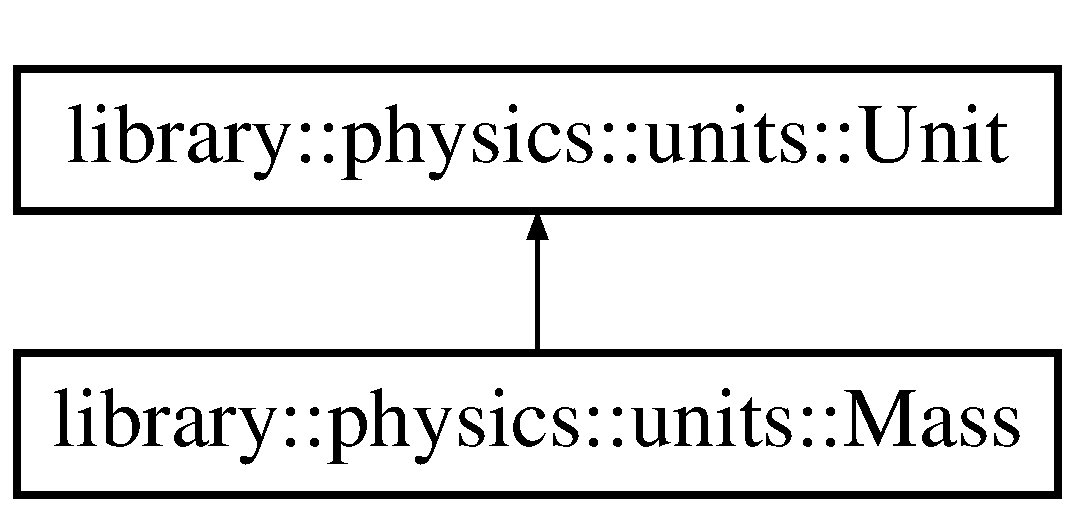
\includegraphics[height=2.000000cm]{classlibrary_1_1physics_1_1units_1_1_mass}
\end{center}
\end{figure}
\subsection*{Public Types}
\begin{DoxyCompactItemize}
\item 
enum \hyperlink{classlibrary_1_1physics_1_1units_1_1_mass_a95f1e0434bc16794926b8e273bc2a54b}{Unit} \{ \hyperlink{classlibrary_1_1physics_1_1units_1_1_mass_a95f1e0434bc16794926b8e273bc2a54baec0fc0100c4fc1ce4eea230c3dc10360}{Unit\+::\+Undefined}, 
\hyperlink{classlibrary_1_1physics_1_1units_1_1_mass_a95f1e0434bc16794926b8e273bc2a54ba9d71f8d145c74f11bf9b02047645bcf4}{Unit\+::\+Kilogram}, 
\hyperlink{classlibrary_1_1physics_1_1units_1_1_mass_a95f1e0434bc16794926b8e273bc2a54ba8cc4e66809c94072df6426c278d7b36b}{Unit\+::\+Tonne}, 
\hyperlink{classlibrary_1_1physics_1_1units_1_1_mass_a95f1e0434bc16794926b8e273bc2a54ba5a9dc6d94a5d29cbb1b5bc104fa23730}{Unit\+::\+Pound}
 \}
\end{DoxyCompactItemize}
\subsection*{Public Member Functions}
\begin{DoxyCompactItemize}
\item 
\hyperlink{classlibrary_1_1physics_1_1units_1_1_mass_a079df004a90cfe6cfa5c00ce0d816122}{Mass} (const Real \&a\+Value, const \hyperlink{classlibrary_1_1physics_1_1units_1_1_mass_a95f1e0434bc16794926b8e273bc2a54b}{Mass\+::\+Unit} \&a\+Unit)
\begin{DoxyCompactList}\small\item\em Constructor. \end{DoxyCompactList}\item 
virtual \hyperlink{classlibrary_1_1physics_1_1units_1_1_mass}{Mass} $\ast$ \hyperlink{classlibrary_1_1physics_1_1units_1_1_mass_a7a09438b05edbe4b21a05ec234a6372f}{clone} () const override
\item 
virtual bool \hyperlink{classlibrary_1_1physics_1_1units_1_1_mass_a0efde6eb08d6b79baa84229746776b6a}{is\+Defined} () const override
\item 
virtual String \hyperlink{classlibrary_1_1physics_1_1units_1_1_mass_a6e7757920752ac9f6918525d6fadb31e}{to\+String} (const Integer \&a\+Precision=Integer\+::\+Undefined()) const override
\end{DoxyCompactItemize}
\subsection*{Static Public Member Functions}
\begin{DoxyCompactItemize}
\item 
static \hyperlink{classlibrary_1_1physics_1_1units_1_1_mass}{Mass} \hyperlink{classlibrary_1_1physics_1_1units_1_1_mass_af3acc8762e8791a218e877595e94090b}{Undefined} ()
\item 
static String \hyperlink{classlibrary_1_1physics_1_1units_1_1_mass_ab2abb07bd20ab0a435b49b494f4ceb3f}{String\+From\+Unit} (const \hyperlink{classlibrary_1_1physics_1_1units_1_1_mass_a95f1e0434bc16794926b8e273bc2a54b}{Mass\+::\+Unit} \&a\+Unit)
\item 
static String \hyperlink{classlibrary_1_1physics_1_1units_1_1_mass_ad61ae35ac949926191b2517e674467a3}{Symbol\+From\+Unit} (const \hyperlink{classlibrary_1_1physics_1_1units_1_1_mass_a95f1e0434bc16794926b8e273bc2a54b}{Mass\+::\+Unit} \&a\+Unit)
\end{DoxyCompactItemize}


\subsection{Detailed Description}
\hyperlink{classlibrary_1_1physics_1_1units_1_1_mass}{Mass}. 

https\+://en.wikipedia.\+org/wiki/\+Mass 

\subsection{Member Enumeration Documentation}
\mbox{\Hypertarget{classlibrary_1_1physics_1_1units_1_1_mass_a95f1e0434bc16794926b8e273bc2a54b}\label{classlibrary_1_1physics_1_1units_1_1_mass_a95f1e0434bc16794926b8e273bc2a54b}} 
\index{library\+::physics\+::units\+::\+Mass@{library\+::physics\+::units\+::\+Mass}!Unit@{Unit}}
\index{Unit@{Unit}!library\+::physics\+::units\+::\+Mass@{library\+::physics\+::units\+::\+Mass}}
\subsubsection{\texorpdfstring{Unit}{Unit}}
{\footnotesize\ttfamily enum \hyperlink{classlibrary_1_1physics_1_1units_1_1_mass_a95f1e0434bc16794926b8e273bc2a54b}{library\+::physics\+::units\+::\+Mass\+::\+Unit}\hspace{0.3cm}{\ttfamily [strong]}}

\begin{DoxyEnumFields}{Enumerator}
\raisebox{\heightof{T}}[0pt][0pt]{\index{Undefined@{Undefined}!library\+::physics\+::units\+::\+Mass@{library\+::physics\+::units\+::\+Mass}}\index{library\+::physics\+::units\+::\+Mass@{library\+::physics\+::units\+::\+Mass}!Undefined@{Undefined}}}\mbox{\Hypertarget{classlibrary_1_1physics_1_1units_1_1_mass_a95f1e0434bc16794926b8e273bc2a54baec0fc0100c4fc1ce4eea230c3dc10360}\label{classlibrary_1_1physics_1_1units_1_1_mass_a95f1e0434bc16794926b8e273bc2a54baec0fc0100c4fc1ce4eea230c3dc10360}} 
Undefined&Undefined. \\
\hline

\raisebox{\heightof{T}}[0pt][0pt]{\index{Kilogram@{Kilogram}!library\+::physics\+::units\+::\+Mass@{library\+::physics\+::units\+::\+Mass}}\index{library\+::physics\+::units\+::\+Mass@{library\+::physics\+::units\+::\+Mass}!Kilogram@{Kilogram}}}\mbox{\Hypertarget{classlibrary_1_1physics_1_1units_1_1_mass_a95f1e0434bc16794926b8e273bc2a54ba9d71f8d145c74f11bf9b02047645bcf4}\label{classlibrary_1_1physics_1_1units_1_1_mass_a95f1e0434bc16794926b8e273bc2a54ba9d71f8d145c74f11bf9b02047645bcf4}} 
Kilogram&Kilogram (SI) \\
\hline

\raisebox{\heightof{T}}[0pt][0pt]{\index{Tonne@{Tonne}!library\+::physics\+::units\+::\+Mass@{library\+::physics\+::units\+::\+Mass}}\index{library\+::physics\+::units\+::\+Mass@{library\+::physics\+::units\+::\+Mass}!Tonne@{Tonne}}}\mbox{\Hypertarget{classlibrary_1_1physics_1_1units_1_1_mass_a95f1e0434bc16794926b8e273bc2a54ba8cc4e66809c94072df6426c278d7b36b}\label{classlibrary_1_1physics_1_1units_1_1_mass_a95f1e0434bc16794926b8e273bc2a54ba8cc4e66809c94072df6426c278d7b36b}} 
Tonne&Tonne. \\
\hline

\raisebox{\heightof{T}}[0pt][0pt]{\index{Pound@{Pound}!library\+::physics\+::units\+::\+Mass@{library\+::physics\+::units\+::\+Mass}}\index{library\+::physics\+::units\+::\+Mass@{library\+::physics\+::units\+::\+Mass}!Pound@{Pound}}}\mbox{\Hypertarget{classlibrary_1_1physics_1_1units_1_1_mass_a95f1e0434bc16794926b8e273bc2a54ba5a9dc6d94a5d29cbb1b5bc104fa23730}\label{classlibrary_1_1physics_1_1units_1_1_mass_a95f1e0434bc16794926b8e273bc2a54ba5a9dc6d94a5d29cbb1b5bc104fa23730}} 
Pound&Pound. \\
\hline

\end{DoxyEnumFields}


\subsection{Constructor \& Destructor Documentation}
\mbox{\Hypertarget{classlibrary_1_1physics_1_1units_1_1_mass_a079df004a90cfe6cfa5c00ce0d816122}\label{classlibrary_1_1physics_1_1units_1_1_mass_a079df004a90cfe6cfa5c00ce0d816122}} 
\index{library\+::physics\+::units\+::\+Mass@{library\+::physics\+::units\+::\+Mass}!Mass@{Mass}}
\index{Mass@{Mass}!library\+::physics\+::units\+::\+Mass@{library\+::physics\+::units\+::\+Mass}}
\subsubsection{\texorpdfstring{Mass()}{Mass()}}
{\footnotesize\ttfamily library\+::physics\+::units\+::\+Mass\+::\+Mass (\begin{DoxyParamCaption}\item[{const Real \&}]{a\+Value,  }\item[{const \hyperlink{classlibrary_1_1physics_1_1units_1_1_mass_a95f1e0434bc16794926b8e273bc2a54b}{Mass\+::\+Unit} \&}]{a\+Unit }\end{DoxyParamCaption})}



Constructor. 


\begin{DoxyCode}
\hyperlink{classlibrary_1_1physics_1_1units_1_1_mass_a079df004a90cfe6cfa5c00ce0d816122}{Mass} mass(1.0, \hyperlink{classlibrary_1_1physics_1_1units_1_1_mass_a95f1e0434bc16794926b8e273bc2a54ba9d71f8d145c74f11bf9b02047645bcf4}{Mass::Unit::Kilogram}) ;
\end{DoxyCode}



\begin{DoxyParams}[1]{Parameters}
\mbox{\tt in}  & {\em a\+Value} & A value \\
\hline
\mbox{\tt in}  & {\em a\+Unit} & A mass unit \\
\hline
\end{DoxyParams}


\subsection{Member Function Documentation}
\mbox{\Hypertarget{classlibrary_1_1physics_1_1units_1_1_mass_a7a09438b05edbe4b21a05ec234a6372f}\label{classlibrary_1_1physics_1_1units_1_1_mass_a7a09438b05edbe4b21a05ec234a6372f}} 
\index{library\+::physics\+::units\+::\+Mass@{library\+::physics\+::units\+::\+Mass}!clone@{clone}}
\index{clone@{clone}!library\+::physics\+::units\+::\+Mass@{library\+::physics\+::units\+::\+Mass}}
\subsubsection{\texorpdfstring{clone()}{clone()}}
{\footnotesize\ttfamily \hyperlink{classlibrary_1_1physics_1_1units_1_1_mass}{Mass} $\ast$ library\+::physics\+::units\+::\+Mass\+::clone (\begin{DoxyParamCaption}{ }\end{DoxyParamCaption}) const\hspace{0.3cm}{\ttfamily [override]}, {\ttfamily [virtual]}}



Implements \hyperlink{classlibrary_1_1physics_1_1units_1_1_unit_aff727141d73acddfae382e5e375f4640}{library\+::physics\+::units\+::\+Unit}.

\mbox{\Hypertarget{classlibrary_1_1physics_1_1units_1_1_mass_a0efde6eb08d6b79baa84229746776b6a}\label{classlibrary_1_1physics_1_1units_1_1_mass_a0efde6eb08d6b79baa84229746776b6a}} 
\index{library\+::physics\+::units\+::\+Mass@{library\+::physics\+::units\+::\+Mass}!is\+Defined@{is\+Defined}}
\index{is\+Defined@{is\+Defined}!library\+::physics\+::units\+::\+Mass@{library\+::physics\+::units\+::\+Mass}}
\subsubsection{\texorpdfstring{is\+Defined()}{isDefined()}}
{\footnotesize\ttfamily bool library\+::physics\+::units\+::\+Mass\+::is\+Defined (\begin{DoxyParamCaption}{ }\end{DoxyParamCaption}) const\hspace{0.3cm}{\ttfamily [override]}, {\ttfamily [virtual]}}



Reimplemented from \hyperlink{classlibrary_1_1physics_1_1units_1_1_unit_a5ce011c1ffa0fce4cf1f5d42ff06ee78}{library\+::physics\+::units\+::\+Unit}.

\mbox{\Hypertarget{classlibrary_1_1physics_1_1units_1_1_mass_ab2abb07bd20ab0a435b49b494f4ceb3f}\label{classlibrary_1_1physics_1_1units_1_1_mass_ab2abb07bd20ab0a435b49b494f4ceb3f}} 
\index{library\+::physics\+::units\+::\+Mass@{library\+::physics\+::units\+::\+Mass}!String\+From\+Unit@{String\+From\+Unit}}
\index{String\+From\+Unit@{String\+From\+Unit}!library\+::physics\+::units\+::\+Mass@{library\+::physics\+::units\+::\+Mass}}
\subsubsection{\texorpdfstring{String\+From\+Unit()}{StringFromUnit()}}
{\footnotesize\ttfamily String library\+::physics\+::units\+::\+Mass\+::\+String\+From\+Unit (\begin{DoxyParamCaption}\item[{const \hyperlink{classlibrary_1_1physics_1_1units_1_1_mass_a95f1e0434bc16794926b8e273bc2a54b}{Mass\+::\+Unit} \&}]{a\+Unit }\end{DoxyParamCaption})\hspace{0.3cm}{\ttfamily [static]}}

\mbox{\Hypertarget{classlibrary_1_1physics_1_1units_1_1_mass_ad61ae35ac949926191b2517e674467a3}\label{classlibrary_1_1physics_1_1units_1_1_mass_ad61ae35ac949926191b2517e674467a3}} 
\index{library\+::physics\+::units\+::\+Mass@{library\+::physics\+::units\+::\+Mass}!Symbol\+From\+Unit@{Symbol\+From\+Unit}}
\index{Symbol\+From\+Unit@{Symbol\+From\+Unit}!library\+::physics\+::units\+::\+Mass@{library\+::physics\+::units\+::\+Mass}}
\subsubsection{\texorpdfstring{Symbol\+From\+Unit()}{SymbolFromUnit()}}
{\footnotesize\ttfamily String library\+::physics\+::units\+::\+Mass\+::\+Symbol\+From\+Unit (\begin{DoxyParamCaption}\item[{const \hyperlink{classlibrary_1_1physics_1_1units_1_1_mass_a95f1e0434bc16794926b8e273bc2a54b}{Mass\+::\+Unit} \&}]{a\+Unit }\end{DoxyParamCaption})\hspace{0.3cm}{\ttfamily [static]}}

\mbox{\Hypertarget{classlibrary_1_1physics_1_1units_1_1_mass_a6e7757920752ac9f6918525d6fadb31e}\label{classlibrary_1_1physics_1_1units_1_1_mass_a6e7757920752ac9f6918525d6fadb31e}} 
\index{library\+::physics\+::units\+::\+Mass@{library\+::physics\+::units\+::\+Mass}!to\+String@{to\+String}}
\index{to\+String@{to\+String}!library\+::physics\+::units\+::\+Mass@{library\+::physics\+::units\+::\+Mass}}
\subsubsection{\texorpdfstring{to\+String()}{toString()}}
{\footnotesize\ttfamily String library\+::physics\+::units\+::\+Mass\+::to\+String (\begin{DoxyParamCaption}\item[{const Integer \&}]{a\+Precision = {\ttfamily Integer\+:\+:Undefined()} }\end{DoxyParamCaption}) const\hspace{0.3cm}{\ttfamily [override]}, {\ttfamily [virtual]}}



Implements \hyperlink{classlibrary_1_1physics_1_1units_1_1_unit_ad7364d457300e36413323c4aebce8029}{library\+::physics\+::units\+::\+Unit}.

\mbox{\Hypertarget{classlibrary_1_1physics_1_1units_1_1_mass_af3acc8762e8791a218e877595e94090b}\label{classlibrary_1_1physics_1_1units_1_1_mass_af3acc8762e8791a218e877595e94090b}} 
\index{library\+::physics\+::units\+::\+Mass@{library\+::physics\+::units\+::\+Mass}!Undefined@{Undefined}}
\index{Undefined@{Undefined}!library\+::physics\+::units\+::\+Mass@{library\+::physics\+::units\+::\+Mass}}
\subsubsection{\texorpdfstring{Undefined()}{Undefined()}}
{\footnotesize\ttfamily \hyperlink{classlibrary_1_1physics_1_1units_1_1_mass}{Mass} library\+::physics\+::units\+::\+Mass\+::\+Undefined (\begin{DoxyParamCaption}{ }\end{DoxyParamCaption})\hspace{0.3cm}{\ttfamily [static]}}



The documentation for this class was generated from the following files\+:\begin{DoxyCompactItemize}
\item 
include/\+Library/\+Physics/\+Units/\hyperlink{_mass_8hpp}{Mass.\+hpp}\item 
src/\+Library/\+Physics/\+Units/\hyperlink{_mass_8cpp}{Mass.\+cpp}\end{DoxyCompactItemize}

\hypertarget{classlibrary_1_1physics_1_1env_1_1obj_1_1celest_1_1_moon}{}\section{library\+:\+:physics\+:\+:env\+:\+:obj\+:\+:celest\+:\+:Moon Class Reference}
\label{classlibrary_1_1physics_1_1env_1_1obj_1_1celest_1_1_moon}\index{library\+::physics\+::env\+::obj\+::celest\+::\+Moon@{library\+::physics\+::env\+::obj\+::celest\+::\+Moon}}


{\ttfamily \#include $<$Moon.\+hpp$>$}

Inheritance diagram for library\+:\+:physics\+:\+:env\+:\+:obj\+:\+:celest\+:\+:Moon\+:\begin{figure}[H]
\begin{center}
\leavevmode
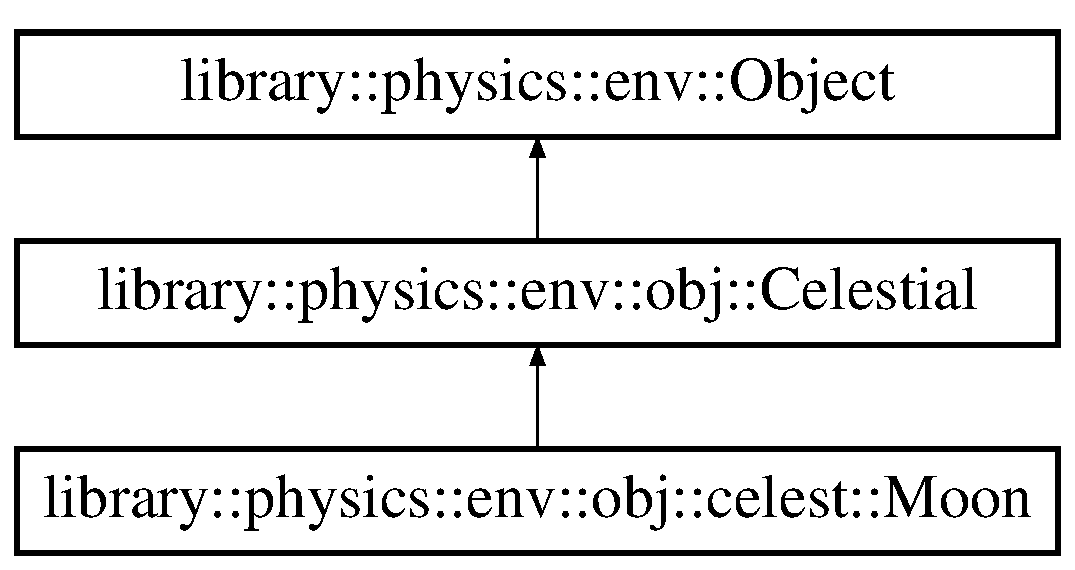
\includegraphics[height=3.000000cm]{classlibrary_1_1physics_1_1env_1_1obj_1_1celest_1_1_moon}
\end{center}
\end{figure}
\subsection*{Public Member Functions}
\begin{DoxyCompactItemize}
\item 
\hyperlink{classlibrary_1_1physics_1_1env_1_1obj_1_1celest_1_1_moon_aa7c19c2d391128ca7f4af52915b11261}{Moon} (const Shared$<$ \hyperlink{classlibrary_1_1physics_1_1env_1_1_ephemeris}{Ephemeris} $>$ \&an\+Ephemeris\+S\+Ptr, const \hyperlink{classlibrary_1_1physics_1_1time_1_1_instant}{Instant} \&an\+Instant)
\item 
virtual \hyperlink{classlibrary_1_1physics_1_1env_1_1obj_1_1celest_1_1_moon_aef4e99355b923e8c41ec12237bf41ecb}{$\sim$\+Moon} () override
\item 
virtual \hyperlink{classlibrary_1_1physics_1_1env_1_1obj_1_1celest_1_1_moon}{Moon} $\ast$ \hyperlink{classlibrary_1_1physics_1_1env_1_1obj_1_1celest_1_1_moon_a9d922ab338809a6c1052edbe11ce3e60}{clone} () const override
\end{DoxyCompactItemize}
\subsection*{Static Public Member Functions}
\begin{DoxyCompactItemize}
\item 
static \hyperlink{classlibrary_1_1physics_1_1env_1_1obj_1_1celest_1_1_moon}{Moon} \hyperlink{classlibrary_1_1physics_1_1env_1_1obj_1_1celest_1_1_moon_a3af7c97ead0a90e481705e74bef0d18d}{Analytical} (const \hyperlink{classlibrary_1_1physics_1_1time_1_1_instant}{Instant} \&an\+Instant)
\end{DoxyCompactItemize}
\subsection*{Static Public Attributes}
\begin{DoxyCompactItemize}
\item 
static \hyperlink{classlibrary_1_1physics_1_1units_1_1_derived}{Derived} \hyperlink{classlibrary_1_1physics_1_1env_1_1obj_1_1celest_1_1_moon_aee16207c53ac86140c994da72cce64d2}{Gravitational\+Constant} = \hyperlink{classlibrary_1_1physics_1_1units_1_1_derived}{Derived}(4902.\+8000e9, \{ Length\+::\+Unit\+::\+Meter, Derived\+::\+Order(3), Mass\+::\+Unit\+::\+Undefined, Derived\+::\+Order\+::\+Zero(), Time\+::\+Unit\+::\+Second, Derived\+::\+Order(-\/2), Angle\+::\+Unit\+::\+Undefined, Derived\+::\+Order\+::\+Zero() \})
\item 
static \hyperlink{classlibrary_1_1physics_1_1units_1_1_length}{Length} \hyperlink{classlibrary_1_1physics_1_1env_1_1obj_1_1celest_1_1_moon_a6b22597902ccee09be70ae4eecca2174}{Equatorial\+Radius} = \hyperlink{classlibrary_1_1physics_1_1units_1_1_length_ad523a3737d5c3f23a64588eac83f2148}{Length\+::\+Meters}(1738.\+14e3)
\item 
static Real \hyperlink{classlibrary_1_1physics_1_1env_1_1obj_1_1celest_1_1_moon_a02e660fcf1bf06697a037a354f698499}{Flattening} = 0.\+00125
\end{DoxyCompactItemize}
\subsection*{Additional Inherited Members}


\subsection{Constructor \& Destructor Documentation}
\mbox{\Hypertarget{classlibrary_1_1physics_1_1env_1_1obj_1_1celest_1_1_moon_aa7c19c2d391128ca7f4af52915b11261}\label{classlibrary_1_1physics_1_1env_1_1obj_1_1celest_1_1_moon_aa7c19c2d391128ca7f4af52915b11261}} 
\index{library\+::physics\+::env\+::obj\+::celest\+::\+Moon@{library\+::physics\+::env\+::obj\+::celest\+::\+Moon}!Moon@{Moon}}
\index{Moon@{Moon}!library\+::physics\+::env\+::obj\+::celest\+::\+Moon@{library\+::physics\+::env\+::obj\+::celest\+::\+Moon}}
\subsubsection{\texorpdfstring{Moon()}{Moon()}}
{\footnotesize\ttfamily library\+::physics\+::env\+::obj\+::celest\+::\+Moon\+::\+Moon (\begin{DoxyParamCaption}\item[{const Shared$<$ \hyperlink{classlibrary_1_1physics_1_1env_1_1_ephemeris}{Ephemeris} $>$ \&}]{an\+Ephemeris\+S\+Ptr,  }\item[{const \hyperlink{classlibrary_1_1physics_1_1time_1_1_instant}{Instant} \&}]{an\+Instant }\end{DoxyParamCaption})}

\mbox{\Hypertarget{classlibrary_1_1physics_1_1env_1_1obj_1_1celest_1_1_moon_aef4e99355b923e8c41ec12237bf41ecb}\label{classlibrary_1_1physics_1_1env_1_1obj_1_1celest_1_1_moon_aef4e99355b923e8c41ec12237bf41ecb}} 
\index{library\+::physics\+::env\+::obj\+::celest\+::\+Moon@{library\+::physics\+::env\+::obj\+::celest\+::\+Moon}!````~Moon@{$\sim$\+Moon}}
\index{````~Moon@{$\sim$\+Moon}!library\+::physics\+::env\+::obj\+::celest\+::\+Moon@{library\+::physics\+::env\+::obj\+::celest\+::\+Moon}}
\subsubsection{\texorpdfstring{$\sim$\+Moon()}{~Moon()}}
{\footnotesize\ttfamily library\+::physics\+::env\+::obj\+::celest\+::\+Moon\+::$\sim$\+Moon (\begin{DoxyParamCaption}{ }\end{DoxyParamCaption})\hspace{0.3cm}{\ttfamily [override]}, {\ttfamily [virtual]}}



\subsection{Member Function Documentation}
\mbox{\Hypertarget{classlibrary_1_1physics_1_1env_1_1obj_1_1celest_1_1_moon_a3af7c97ead0a90e481705e74bef0d18d}\label{classlibrary_1_1physics_1_1env_1_1obj_1_1celest_1_1_moon_a3af7c97ead0a90e481705e74bef0d18d}} 
\index{library\+::physics\+::env\+::obj\+::celest\+::\+Moon@{library\+::physics\+::env\+::obj\+::celest\+::\+Moon}!Analytical@{Analytical}}
\index{Analytical@{Analytical}!library\+::physics\+::env\+::obj\+::celest\+::\+Moon@{library\+::physics\+::env\+::obj\+::celest\+::\+Moon}}
\subsubsection{\texorpdfstring{Analytical()}{Analytical()}}
{\footnotesize\ttfamily \hyperlink{classlibrary_1_1physics_1_1env_1_1obj_1_1celest_1_1_moon}{Moon} library\+::physics\+::env\+::obj\+::celest\+::\+Moon\+::\+Analytical (\begin{DoxyParamCaption}\item[{const \hyperlink{classlibrary_1_1physics_1_1time_1_1_instant}{Instant} \&}]{an\+Instant }\end{DoxyParamCaption})\hspace{0.3cm}{\ttfamily [static]}}

\mbox{\Hypertarget{classlibrary_1_1physics_1_1env_1_1obj_1_1celest_1_1_moon_a9d922ab338809a6c1052edbe11ce3e60}\label{classlibrary_1_1physics_1_1env_1_1obj_1_1celest_1_1_moon_a9d922ab338809a6c1052edbe11ce3e60}} 
\index{library\+::physics\+::env\+::obj\+::celest\+::\+Moon@{library\+::physics\+::env\+::obj\+::celest\+::\+Moon}!clone@{clone}}
\index{clone@{clone}!library\+::physics\+::env\+::obj\+::celest\+::\+Moon@{library\+::physics\+::env\+::obj\+::celest\+::\+Moon}}
\subsubsection{\texorpdfstring{clone()}{clone()}}
{\footnotesize\ttfamily \hyperlink{classlibrary_1_1physics_1_1env_1_1obj_1_1celest_1_1_moon}{Moon} $\ast$ library\+::physics\+::env\+::obj\+::celest\+::\+Moon\+::clone (\begin{DoxyParamCaption}{ }\end{DoxyParamCaption}) const\hspace{0.3cm}{\ttfamily [override]}, {\ttfamily [virtual]}}



Reimplemented from \hyperlink{classlibrary_1_1physics_1_1env_1_1obj_1_1_celestial_aaf8aa41a0ff9336eba62c07e3c27f82d}{library\+::physics\+::env\+::obj\+::\+Celestial}.



\subsection{Member Data Documentation}
\mbox{\Hypertarget{classlibrary_1_1physics_1_1env_1_1obj_1_1celest_1_1_moon_a6b22597902ccee09be70ae4eecca2174}\label{classlibrary_1_1physics_1_1env_1_1obj_1_1celest_1_1_moon_a6b22597902ccee09be70ae4eecca2174}} 
\index{library\+::physics\+::env\+::obj\+::celest\+::\+Moon@{library\+::physics\+::env\+::obj\+::celest\+::\+Moon}!Equatorial\+Radius@{Equatorial\+Radius}}
\index{Equatorial\+Radius@{Equatorial\+Radius}!library\+::physics\+::env\+::obj\+::celest\+::\+Moon@{library\+::physics\+::env\+::obj\+::celest\+::\+Moon}}
\subsubsection{\texorpdfstring{Equatorial\+Radius}{EquatorialRadius}}
{\footnotesize\ttfamily \hyperlink{classlibrary_1_1physics_1_1units_1_1_length}{Length} library\+::physics\+::env\+::obj\+::celest\+::\+Moon\+::\+Equatorial\+Radius = \hyperlink{classlibrary_1_1physics_1_1units_1_1_length_ad523a3737d5c3f23a64588eac83f2148}{Length\+::\+Meters}(1738.\+14e3)\hspace{0.3cm}{\ttfamily [static]}}

\mbox{\Hypertarget{classlibrary_1_1physics_1_1env_1_1obj_1_1celest_1_1_moon_a02e660fcf1bf06697a037a354f698499}\label{classlibrary_1_1physics_1_1env_1_1obj_1_1celest_1_1_moon_a02e660fcf1bf06697a037a354f698499}} 
\index{library\+::physics\+::env\+::obj\+::celest\+::\+Moon@{library\+::physics\+::env\+::obj\+::celest\+::\+Moon}!Flattening@{Flattening}}
\index{Flattening@{Flattening}!library\+::physics\+::env\+::obj\+::celest\+::\+Moon@{library\+::physics\+::env\+::obj\+::celest\+::\+Moon}}
\subsubsection{\texorpdfstring{Flattening}{Flattening}}
{\footnotesize\ttfamily Real library\+::physics\+::env\+::obj\+::celest\+::\+Moon\+::\+Flattening = 0.\+00125\hspace{0.3cm}{\ttfamily [static]}}

\mbox{\Hypertarget{classlibrary_1_1physics_1_1env_1_1obj_1_1celest_1_1_moon_aee16207c53ac86140c994da72cce64d2}\label{classlibrary_1_1physics_1_1env_1_1obj_1_1celest_1_1_moon_aee16207c53ac86140c994da72cce64d2}} 
\index{library\+::physics\+::env\+::obj\+::celest\+::\+Moon@{library\+::physics\+::env\+::obj\+::celest\+::\+Moon}!Gravitational\+Constant@{Gravitational\+Constant}}
\index{Gravitational\+Constant@{Gravitational\+Constant}!library\+::physics\+::env\+::obj\+::celest\+::\+Moon@{library\+::physics\+::env\+::obj\+::celest\+::\+Moon}}
\subsubsection{\texorpdfstring{Gravitational\+Constant}{GravitationalConstant}}
{\footnotesize\ttfamily \hyperlink{classlibrary_1_1physics_1_1units_1_1_derived}{Derived} library\+::physics\+::env\+::obj\+::celest\+::\+Moon\+::\+Gravitational\+Constant = \hyperlink{classlibrary_1_1physics_1_1units_1_1_derived}{Derived}(4902.\+8000e9, \{ Length\+::\+Unit\+::\+Meter, Derived\+::\+Order(3), Mass\+::\+Unit\+::\+Undefined, Derived\+::\+Order\+::\+Zero(), Time\+::\+Unit\+::\+Second, Derived\+::\+Order(-\/2), Angle\+::\+Unit\+::\+Undefined, Derived\+::\+Order\+::\+Zero() \})\hspace{0.3cm}{\ttfamily [static]}}



The documentation for this class was generated from the following files\+:\begin{DoxyCompactItemize}
\item 
include/\+Library/\+Physics/\+Environment/\+Objects/\+Celestial\+Bodies/\hyperlink{_moon_8hpp}{Moon.\+hpp}\item 
src/\+Library/\+Physics/\+Environment/\+Objects/\+Celestial\+Bodies/\hyperlink{_moon_8cpp}{Moon.\+cpp}\end{DoxyCompactItemize}

\hypertarget{classlibrary_1_1physics_1_1env_1_1_object}{}\section{library\+:\+:physics\+:\+:env\+:\+:Object Class Reference}
\label{classlibrary_1_1physics_1_1env_1_1_object}\index{library\+::physics\+::env\+::\+Object@{library\+::physics\+::env\+::\+Object}}


{\ttfamily \#include $<$Object.\+hpp$>$}

Inheritance diagram for library\+:\+:physics\+:\+:env\+:\+:Object\+:\begin{figure}[H]
\begin{center}
\leavevmode
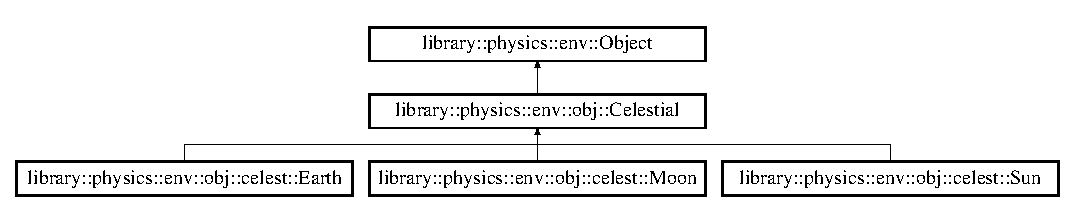
\includegraphics[height=3.000000cm]{classlibrary_1_1physics_1_1env_1_1_object}
\end{center}
\end{figure}
\subsection*{Public Types}
\begin{DoxyCompactItemize}
\item 
typedef \hyperlink{classlibrary_1_1physics_1_1env_1_1object_1_1_geometry}{object\+::\+Geometry} \hyperlink{classlibrary_1_1physics_1_1env_1_1_object_abdf50733c7ad97327fb64edca5670f13}{Geometry}
\end{DoxyCompactItemize}
\subsection*{Public Member Functions}
\begin{DoxyCompactItemize}
\item 
\hyperlink{classlibrary_1_1physics_1_1env_1_1_object_af112257aa51a94dcc61a36e2c0db4b05}{Object} (const String \&a\+Name, const \hyperlink{classlibrary_1_1physics_1_1time_1_1_instant}{Instant} \&an\+Instant)
\item 
\hyperlink{classlibrary_1_1physics_1_1env_1_1_object_a37e5ddc8f0b89e006025a7ac6ac71fe5}{Object} (const String \&a\+Name, const \hyperlink{classlibrary_1_1physics_1_1time_1_1_instant}{Instant} \&an\+Instant, const \hyperlink{classlibrary_1_1physics_1_1env_1_1_object_abdf50733c7ad97327fb64edca5670f13}{Object\+::\+Geometry} \&a\+Geometry)
\item 
\hyperlink{classlibrary_1_1physics_1_1env_1_1_object_ac7b0b65eb0f2a65a46314269687ad49e}{Object} (const \hyperlink{classlibrary_1_1physics_1_1env_1_1_object}{Object} \&an\+Object)
\item 
virtual \hyperlink{classlibrary_1_1physics_1_1env_1_1_object_a2b48d75c2f1a01e2808e9efe4fe68393}{$\sim$\+Object} ()=0
\item 
virtual \hyperlink{classlibrary_1_1physics_1_1env_1_1_object}{Object} $\ast$ \hyperlink{classlibrary_1_1physics_1_1env_1_1_object_a498e0d1a15e937a5aa77374c6f899768}{clone} () const =0
\item 
\hyperlink{classlibrary_1_1physics_1_1env_1_1_object}{Object} \& \hyperlink{classlibrary_1_1physics_1_1env_1_1_object_a1e7d9e24f984bcc13e89625805ae15aa}{operator=} (const \hyperlink{classlibrary_1_1physics_1_1env_1_1_object}{Object} \&an\+Object)
\item 
virtual bool \hyperlink{classlibrary_1_1physics_1_1env_1_1_object_a7035edc921681401ddd43b094645a024}{is\+Defined} () const
\item 
const String \& \hyperlink{classlibrary_1_1physics_1_1env_1_1_object_a0cf28bef038e493ee0771680976f5e28}{access\+Name} () const
\item 
const \hyperlink{classlibrary_1_1physics_1_1time_1_1_instant}{Instant} \& \hyperlink{classlibrary_1_1physics_1_1env_1_1_object_a3f183331fd0ad20e88cae41e2491a5dc}{access\+Instant} () const
\item 
virtual Shared$<$ const \hyperlink{classlibrary_1_1physics_1_1coord_1_1_frame}{Frame} $>$ \hyperlink{classlibrary_1_1physics_1_1env_1_1_object_a6ff59bc7375388118c60b5823dad748b}{access\+Frame} () const =0
\item 
const \hyperlink{classlibrary_1_1physics_1_1env_1_1_object_abdf50733c7ad97327fb64edca5670f13}{Object\+::\+Geometry} \& \hyperlink{classlibrary_1_1physics_1_1env_1_1_object_ac7a98e912dadb573e557eb91c8f5e891}{access\+Geometry} () const
\item 
String \hyperlink{classlibrary_1_1physics_1_1env_1_1_object_ab9c4454cd7beb5a5bab5f888c0ea2f1f}{get\+Name} () const
\item 
\hyperlink{classlibrary_1_1physics_1_1time_1_1_instant}{Instant} \hyperlink{classlibrary_1_1physics_1_1env_1_1_object_a8ca9c7efb9fee9196e23d660c46adac0}{get\+Instant} () const
\item 
\hyperlink{classlibrary_1_1physics_1_1env_1_1_object_abdf50733c7ad97327fb64edca5670f13}{Object\+::\+Geometry} \hyperlink{classlibrary_1_1physics_1_1env_1_1_object_a504f76c6e6da18b531972e6f26329255}{get\+Geometry} () const
\item 
virtual \hyperlink{classlibrary_1_1physics_1_1coord_1_1_position}{Position} \hyperlink{classlibrary_1_1physics_1_1env_1_1_object_acc86d12ad94de870fc2684f7b768b617}{get\+Position\+In} (const Shared$<$ const \hyperlink{classlibrary_1_1physics_1_1coord_1_1_frame}{Frame} $>$ \&a\+Frame\+S\+Ptr) const =0
\item 
virtual \hyperlink{classlibrary_1_1physics_1_1coord_1_1_velocity}{Velocity} \hyperlink{classlibrary_1_1physics_1_1env_1_1_object_a1a8f4358db37b1b8830866373f8f3670}{get\+Velocity\+In} (const Shared$<$ const \hyperlink{classlibrary_1_1physics_1_1coord_1_1_frame}{Frame} $>$ \&a\+Frame\+S\+Ptr) const =0
\item 
virtual \hyperlink{classlibrary_1_1physics_1_1coord_1_1_transform}{Transform} \hyperlink{classlibrary_1_1physics_1_1env_1_1_object_abe850e2334c19ae185456cd52aeeca7d}{get\+Transform\+To} (const Shared$<$ const \hyperlink{classlibrary_1_1physics_1_1coord_1_1_frame}{Frame} $>$ \&a\+Frame\+S\+Ptr) const =0
\item 
virtual \hyperlink{classlibrary_1_1physics_1_1coord_1_1_axes}{Axes} \hyperlink{classlibrary_1_1physics_1_1env_1_1_object_a6807199a92fd78c10c6327b9ca654f50}{get\+Axes\+In} (const Shared$<$ const \hyperlink{classlibrary_1_1physics_1_1coord_1_1_frame}{Frame} $>$ \&a\+Frame\+S\+Ptr) const =0
\item 
\hyperlink{classlibrary_1_1physics_1_1env_1_1_object_abdf50733c7ad97327fb64edca5670f13}{Object\+::\+Geometry} \hyperlink{classlibrary_1_1physics_1_1env_1_1_object_a199472d1b6a3b6a3b1694aaddc7b3046}{get\+Geometry\+In} (const Shared$<$ const \hyperlink{classlibrary_1_1physics_1_1coord_1_1_frame}{Frame} $>$ \&a\+Frame\+S\+Ptr) const
\item 
void \hyperlink{classlibrary_1_1physics_1_1env_1_1_object_a6a215fef40593ef3dae3bf2b681339d2}{set\+Instant} (const \hyperlink{classlibrary_1_1physics_1_1time_1_1_instant}{Instant} \&an\+Instant)
\end{DoxyCompactItemize}
\subsection*{Friends}
\begin{DoxyCompactItemize}
\item 
std\+::ostream \& \hyperlink{classlibrary_1_1physics_1_1env_1_1_object_a418df9bf4a73078f3d494edef1743f8d}{operator$<$$<$} (std\+::ostream \&an\+Output\+Stream, const \hyperlink{classlibrary_1_1physics_1_1env_1_1_object}{Object} \&an\+Object)
\end{DoxyCompactItemize}


\subsection{Member Typedef Documentation}
\mbox{\Hypertarget{classlibrary_1_1physics_1_1env_1_1_object_abdf50733c7ad97327fb64edca5670f13}\label{classlibrary_1_1physics_1_1env_1_1_object_abdf50733c7ad97327fb64edca5670f13}} 
\index{library\+::physics\+::env\+::\+Object@{library\+::physics\+::env\+::\+Object}!Geometry@{Geometry}}
\index{Geometry@{Geometry}!library\+::physics\+::env\+::\+Object@{library\+::physics\+::env\+::\+Object}}
\subsubsection{\texorpdfstring{Geometry}{Geometry}}
{\footnotesize\ttfamily typedef \hyperlink{classlibrary_1_1physics_1_1env_1_1object_1_1_geometry}{object\+::\+Geometry} \hyperlink{classlibrary_1_1physics_1_1env_1_1_object_abdf50733c7ad97327fb64edca5670f13}{library\+::physics\+::env\+::\+Object\+::\+Geometry}}



\subsection{Constructor \& Destructor Documentation}
\mbox{\Hypertarget{classlibrary_1_1physics_1_1env_1_1_object_af112257aa51a94dcc61a36e2c0db4b05}\label{classlibrary_1_1physics_1_1env_1_1_object_af112257aa51a94dcc61a36e2c0db4b05}} 
\index{library\+::physics\+::env\+::\+Object@{library\+::physics\+::env\+::\+Object}!Object@{Object}}
\index{Object@{Object}!library\+::physics\+::env\+::\+Object@{library\+::physics\+::env\+::\+Object}}
\subsubsection{\texorpdfstring{Object()}{Object()}\hspace{0.1cm}{\footnotesize\ttfamily [1/3]}}
{\footnotesize\ttfamily library\+::physics\+::env\+::\+Object\+::\+Object (\begin{DoxyParamCaption}\item[{const String \&}]{a\+Name,  }\item[{const \hyperlink{classlibrary_1_1physics_1_1time_1_1_instant}{Instant} \&}]{an\+Instant }\end{DoxyParamCaption})}

\mbox{\Hypertarget{classlibrary_1_1physics_1_1env_1_1_object_a37e5ddc8f0b89e006025a7ac6ac71fe5}\label{classlibrary_1_1physics_1_1env_1_1_object_a37e5ddc8f0b89e006025a7ac6ac71fe5}} 
\index{library\+::physics\+::env\+::\+Object@{library\+::physics\+::env\+::\+Object}!Object@{Object}}
\index{Object@{Object}!library\+::physics\+::env\+::\+Object@{library\+::physics\+::env\+::\+Object}}
\subsubsection{\texorpdfstring{Object()}{Object()}\hspace{0.1cm}{\footnotesize\ttfamily [2/3]}}
{\footnotesize\ttfamily library\+::physics\+::env\+::\+Object\+::\+Object (\begin{DoxyParamCaption}\item[{const String \&}]{a\+Name,  }\item[{const \hyperlink{classlibrary_1_1physics_1_1time_1_1_instant}{Instant} \&}]{an\+Instant,  }\item[{const \hyperlink{classlibrary_1_1physics_1_1env_1_1_object_abdf50733c7ad97327fb64edca5670f13}{Object\+::\+Geometry} \&}]{a\+Geometry }\end{DoxyParamCaption})}

\mbox{\Hypertarget{classlibrary_1_1physics_1_1env_1_1_object_ac7b0b65eb0f2a65a46314269687ad49e}\label{classlibrary_1_1physics_1_1env_1_1_object_ac7b0b65eb0f2a65a46314269687ad49e}} 
\index{library\+::physics\+::env\+::\+Object@{library\+::physics\+::env\+::\+Object}!Object@{Object}}
\index{Object@{Object}!library\+::physics\+::env\+::\+Object@{library\+::physics\+::env\+::\+Object}}
\subsubsection{\texorpdfstring{Object()}{Object()}\hspace{0.1cm}{\footnotesize\ttfamily [3/3]}}
{\footnotesize\ttfamily library\+::physics\+::env\+::\+Object\+::\+Object (\begin{DoxyParamCaption}\item[{const \hyperlink{classlibrary_1_1physics_1_1env_1_1_object}{Object} \&}]{an\+Object }\end{DoxyParamCaption})}

\mbox{\Hypertarget{classlibrary_1_1physics_1_1env_1_1_object_a2b48d75c2f1a01e2808e9efe4fe68393}\label{classlibrary_1_1physics_1_1env_1_1_object_a2b48d75c2f1a01e2808e9efe4fe68393}} 
\index{library\+::physics\+::env\+::\+Object@{library\+::physics\+::env\+::\+Object}!````~Object@{$\sim$\+Object}}
\index{````~Object@{$\sim$\+Object}!library\+::physics\+::env\+::\+Object@{library\+::physics\+::env\+::\+Object}}
\subsubsection{\texorpdfstring{$\sim$\+Object()}{~Object()}}
{\footnotesize\ttfamily library\+::physics\+::env\+::\+Object\+::$\sim$\+Object (\begin{DoxyParamCaption}{ }\end{DoxyParamCaption})\hspace{0.3cm}{\ttfamily [pure virtual]}}



\subsection{Member Function Documentation}
\mbox{\Hypertarget{classlibrary_1_1physics_1_1env_1_1_object_a6ff59bc7375388118c60b5823dad748b}\label{classlibrary_1_1physics_1_1env_1_1_object_a6ff59bc7375388118c60b5823dad748b}} 
\index{library\+::physics\+::env\+::\+Object@{library\+::physics\+::env\+::\+Object}!access\+Frame@{access\+Frame}}
\index{access\+Frame@{access\+Frame}!library\+::physics\+::env\+::\+Object@{library\+::physics\+::env\+::\+Object}}
\subsubsection{\texorpdfstring{access\+Frame()}{accessFrame()}}
{\footnotesize\ttfamily virtual Shared$<$const \hyperlink{classlibrary_1_1physics_1_1coord_1_1_frame}{Frame}$>$ library\+::physics\+::env\+::\+Object\+::access\+Frame (\begin{DoxyParamCaption}{ }\end{DoxyParamCaption}) const\hspace{0.3cm}{\ttfamily [pure virtual]}}



Implemented in \hyperlink{classlibrary_1_1physics_1_1env_1_1obj_1_1_celestial_a6649bfe0bf0795aa4def046a8c38aef5}{library\+::physics\+::env\+::obj\+::\+Celestial}.

\mbox{\Hypertarget{classlibrary_1_1physics_1_1env_1_1_object_ac7a98e912dadb573e557eb91c8f5e891}\label{classlibrary_1_1physics_1_1env_1_1_object_ac7a98e912dadb573e557eb91c8f5e891}} 
\index{library\+::physics\+::env\+::\+Object@{library\+::physics\+::env\+::\+Object}!access\+Geometry@{access\+Geometry}}
\index{access\+Geometry@{access\+Geometry}!library\+::physics\+::env\+::\+Object@{library\+::physics\+::env\+::\+Object}}
\subsubsection{\texorpdfstring{access\+Geometry()}{accessGeometry()}}
{\footnotesize\ttfamily const \hyperlink{classlibrary_1_1physics_1_1env_1_1_object_abdf50733c7ad97327fb64edca5670f13}{Object\+::\+Geometry} \& library\+::physics\+::env\+::\+Object\+::access\+Geometry (\begin{DoxyParamCaption}{ }\end{DoxyParamCaption}) const}

\mbox{\Hypertarget{classlibrary_1_1physics_1_1env_1_1_object_a3f183331fd0ad20e88cae41e2491a5dc}\label{classlibrary_1_1physics_1_1env_1_1_object_a3f183331fd0ad20e88cae41e2491a5dc}} 
\index{library\+::physics\+::env\+::\+Object@{library\+::physics\+::env\+::\+Object}!access\+Instant@{access\+Instant}}
\index{access\+Instant@{access\+Instant}!library\+::physics\+::env\+::\+Object@{library\+::physics\+::env\+::\+Object}}
\subsubsection{\texorpdfstring{access\+Instant()}{accessInstant()}}
{\footnotesize\ttfamily const \hyperlink{classlibrary_1_1physics_1_1time_1_1_instant}{Instant} \& library\+::physics\+::env\+::\+Object\+::access\+Instant (\begin{DoxyParamCaption}{ }\end{DoxyParamCaption}) const}

\mbox{\Hypertarget{classlibrary_1_1physics_1_1env_1_1_object_a0cf28bef038e493ee0771680976f5e28}\label{classlibrary_1_1physics_1_1env_1_1_object_a0cf28bef038e493ee0771680976f5e28}} 
\index{library\+::physics\+::env\+::\+Object@{library\+::physics\+::env\+::\+Object}!access\+Name@{access\+Name}}
\index{access\+Name@{access\+Name}!library\+::physics\+::env\+::\+Object@{library\+::physics\+::env\+::\+Object}}
\subsubsection{\texorpdfstring{access\+Name()}{accessName()}}
{\footnotesize\ttfamily const String \& library\+::physics\+::env\+::\+Object\+::access\+Name (\begin{DoxyParamCaption}{ }\end{DoxyParamCaption}) const}

\mbox{\Hypertarget{classlibrary_1_1physics_1_1env_1_1_object_a498e0d1a15e937a5aa77374c6f899768}\label{classlibrary_1_1physics_1_1env_1_1_object_a498e0d1a15e937a5aa77374c6f899768}} 
\index{library\+::physics\+::env\+::\+Object@{library\+::physics\+::env\+::\+Object}!clone@{clone}}
\index{clone@{clone}!library\+::physics\+::env\+::\+Object@{library\+::physics\+::env\+::\+Object}}
\subsubsection{\texorpdfstring{clone()}{clone()}}
{\footnotesize\ttfamily virtual \hyperlink{classlibrary_1_1physics_1_1env_1_1_object}{Object}$\ast$ library\+::physics\+::env\+::\+Object\+::clone (\begin{DoxyParamCaption}{ }\end{DoxyParamCaption}) const\hspace{0.3cm}{\ttfamily [pure virtual]}}



Implemented in \hyperlink{classlibrary_1_1physics_1_1env_1_1obj_1_1_celestial_aaf8aa41a0ff9336eba62c07e3c27f82d}{library\+::physics\+::env\+::obj\+::\+Celestial}, \hyperlink{classlibrary_1_1physics_1_1env_1_1obj_1_1celest_1_1_earth_aca39bec00a2046a3fcef9bf22be52428}{library\+::physics\+::env\+::obj\+::celest\+::\+Earth}, and \hyperlink{classlibrary_1_1physics_1_1env_1_1obj_1_1celest_1_1_moon_a9d922ab338809a6c1052edbe11ce3e60}{library\+::physics\+::env\+::obj\+::celest\+::\+Moon}.

\mbox{\Hypertarget{classlibrary_1_1physics_1_1env_1_1_object_a6807199a92fd78c10c6327b9ca654f50}\label{classlibrary_1_1physics_1_1env_1_1_object_a6807199a92fd78c10c6327b9ca654f50}} 
\index{library\+::physics\+::env\+::\+Object@{library\+::physics\+::env\+::\+Object}!get\+Axes\+In@{get\+Axes\+In}}
\index{get\+Axes\+In@{get\+Axes\+In}!library\+::physics\+::env\+::\+Object@{library\+::physics\+::env\+::\+Object}}
\subsubsection{\texorpdfstring{get\+Axes\+In()}{getAxesIn()}}
{\footnotesize\ttfamily virtual \hyperlink{classlibrary_1_1physics_1_1coord_1_1_axes}{Axes} library\+::physics\+::env\+::\+Object\+::get\+Axes\+In (\begin{DoxyParamCaption}\item[{const Shared$<$ const \hyperlink{classlibrary_1_1physics_1_1coord_1_1_frame}{Frame} $>$ \&}]{a\+Frame\+S\+Ptr }\end{DoxyParamCaption}) const\hspace{0.3cm}{\ttfamily [pure virtual]}}



Implemented in \hyperlink{classlibrary_1_1physics_1_1env_1_1obj_1_1_celestial_a51d7ed3c0dcf627fbbcd81f9b190fb6b}{library\+::physics\+::env\+::obj\+::\+Celestial}.

\mbox{\Hypertarget{classlibrary_1_1physics_1_1env_1_1_object_a504f76c6e6da18b531972e6f26329255}\label{classlibrary_1_1physics_1_1env_1_1_object_a504f76c6e6da18b531972e6f26329255}} 
\index{library\+::physics\+::env\+::\+Object@{library\+::physics\+::env\+::\+Object}!get\+Geometry@{get\+Geometry}}
\index{get\+Geometry@{get\+Geometry}!library\+::physics\+::env\+::\+Object@{library\+::physics\+::env\+::\+Object}}
\subsubsection{\texorpdfstring{get\+Geometry()}{getGeometry()}}
{\footnotesize\ttfamily \hyperlink{classlibrary_1_1physics_1_1env_1_1_object_abdf50733c7ad97327fb64edca5670f13}{Object\+::\+Geometry} library\+::physics\+::env\+::\+Object\+::get\+Geometry (\begin{DoxyParamCaption}{ }\end{DoxyParamCaption}) const}

\mbox{\Hypertarget{classlibrary_1_1physics_1_1env_1_1_object_a199472d1b6a3b6a3b1694aaddc7b3046}\label{classlibrary_1_1physics_1_1env_1_1_object_a199472d1b6a3b6a3b1694aaddc7b3046}} 
\index{library\+::physics\+::env\+::\+Object@{library\+::physics\+::env\+::\+Object}!get\+Geometry\+In@{get\+Geometry\+In}}
\index{get\+Geometry\+In@{get\+Geometry\+In}!library\+::physics\+::env\+::\+Object@{library\+::physics\+::env\+::\+Object}}
\subsubsection{\texorpdfstring{get\+Geometry\+In()}{getGeometryIn()}}
{\footnotesize\ttfamily \hyperlink{classlibrary_1_1physics_1_1env_1_1_object_abdf50733c7ad97327fb64edca5670f13}{Object\+::\+Geometry} library\+::physics\+::env\+::\+Object\+::get\+Geometry\+In (\begin{DoxyParamCaption}\item[{const Shared$<$ const \hyperlink{classlibrary_1_1physics_1_1coord_1_1_frame}{Frame} $>$ \&}]{a\+Frame\+S\+Ptr }\end{DoxyParamCaption}) const}

\mbox{\Hypertarget{classlibrary_1_1physics_1_1env_1_1_object_a8ca9c7efb9fee9196e23d660c46adac0}\label{classlibrary_1_1physics_1_1env_1_1_object_a8ca9c7efb9fee9196e23d660c46adac0}} 
\index{library\+::physics\+::env\+::\+Object@{library\+::physics\+::env\+::\+Object}!get\+Instant@{get\+Instant}}
\index{get\+Instant@{get\+Instant}!library\+::physics\+::env\+::\+Object@{library\+::physics\+::env\+::\+Object}}
\subsubsection{\texorpdfstring{get\+Instant()}{getInstant()}}
{\footnotesize\ttfamily \hyperlink{classlibrary_1_1physics_1_1time_1_1_instant}{Instant} library\+::physics\+::env\+::\+Object\+::get\+Instant (\begin{DoxyParamCaption}{ }\end{DoxyParamCaption}) const}

\mbox{\Hypertarget{classlibrary_1_1physics_1_1env_1_1_object_ab9c4454cd7beb5a5bab5f888c0ea2f1f}\label{classlibrary_1_1physics_1_1env_1_1_object_ab9c4454cd7beb5a5bab5f888c0ea2f1f}} 
\index{library\+::physics\+::env\+::\+Object@{library\+::physics\+::env\+::\+Object}!get\+Name@{get\+Name}}
\index{get\+Name@{get\+Name}!library\+::physics\+::env\+::\+Object@{library\+::physics\+::env\+::\+Object}}
\subsubsection{\texorpdfstring{get\+Name()}{getName()}}
{\footnotesize\ttfamily String library\+::physics\+::env\+::\+Object\+::get\+Name (\begin{DoxyParamCaption}{ }\end{DoxyParamCaption}) const}

\mbox{\Hypertarget{classlibrary_1_1physics_1_1env_1_1_object_acc86d12ad94de870fc2684f7b768b617}\label{classlibrary_1_1physics_1_1env_1_1_object_acc86d12ad94de870fc2684f7b768b617}} 
\index{library\+::physics\+::env\+::\+Object@{library\+::physics\+::env\+::\+Object}!get\+Position\+In@{get\+Position\+In}}
\index{get\+Position\+In@{get\+Position\+In}!library\+::physics\+::env\+::\+Object@{library\+::physics\+::env\+::\+Object}}
\subsubsection{\texorpdfstring{get\+Position\+In()}{getPositionIn()}}
{\footnotesize\ttfamily virtual \hyperlink{classlibrary_1_1physics_1_1coord_1_1_position}{Position} library\+::physics\+::env\+::\+Object\+::get\+Position\+In (\begin{DoxyParamCaption}\item[{const Shared$<$ const \hyperlink{classlibrary_1_1physics_1_1coord_1_1_frame}{Frame} $>$ \&}]{a\+Frame\+S\+Ptr }\end{DoxyParamCaption}) const\hspace{0.3cm}{\ttfamily [pure virtual]}}



Implemented in \hyperlink{classlibrary_1_1physics_1_1env_1_1obj_1_1_celestial_aa2a209f37414e24303c21d994396664f}{library\+::physics\+::env\+::obj\+::\+Celestial}.

\mbox{\Hypertarget{classlibrary_1_1physics_1_1env_1_1_object_abe850e2334c19ae185456cd52aeeca7d}\label{classlibrary_1_1physics_1_1env_1_1_object_abe850e2334c19ae185456cd52aeeca7d}} 
\index{library\+::physics\+::env\+::\+Object@{library\+::physics\+::env\+::\+Object}!get\+Transform\+To@{get\+Transform\+To}}
\index{get\+Transform\+To@{get\+Transform\+To}!library\+::physics\+::env\+::\+Object@{library\+::physics\+::env\+::\+Object}}
\subsubsection{\texorpdfstring{get\+Transform\+To()}{getTransformTo()}}
{\footnotesize\ttfamily virtual \hyperlink{classlibrary_1_1physics_1_1coord_1_1_transform}{Transform} library\+::physics\+::env\+::\+Object\+::get\+Transform\+To (\begin{DoxyParamCaption}\item[{const Shared$<$ const \hyperlink{classlibrary_1_1physics_1_1coord_1_1_frame}{Frame} $>$ \&}]{a\+Frame\+S\+Ptr }\end{DoxyParamCaption}) const\hspace{0.3cm}{\ttfamily [pure virtual]}}



Implemented in \hyperlink{classlibrary_1_1physics_1_1env_1_1obj_1_1_celestial_ac6676b10ebbb63a8483137c9c734c58a}{library\+::physics\+::env\+::obj\+::\+Celestial}.

\mbox{\Hypertarget{classlibrary_1_1physics_1_1env_1_1_object_a1a8f4358db37b1b8830866373f8f3670}\label{classlibrary_1_1physics_1_1env_1_1_object_a1a8f4358db37b1b8830866373f8f3670}} 
\index{library\+::physics\+::env\+::\+Object@{library\+::physics\+::env\+::\+Object}!get\+Velocity\+In@{get\+Velocity\+In}}
\index{get\+Velocity\+In@{get\+Velocity\+In}!library\+::physics\+::env\+::\+Object@{library\+::physics\+::env\+::\+Object}}
\subsubsection{\texorpdfstring{get\+Velocity\+In()}{getVelocityIn()}}
{\footnotesize\ttfamily virtual \hyperlink{classlibrary_1_1physics_1_1coord_1_1_velocity}{Velocity} library\+::physics\+::env\+::\+Object\+::get\+Velocity\+In (\begin{DoxyParamCaption}\item[{const Shared$<$ const \hyperlink{classlibrary_1_1physics_1_1coord_1_1_frame}{Frame} $>$ \&}]{a\+Frame\+S\+Ptr }\end{DoxyParamCaption}) const\hspace{0.3cm}{\ttfamily [pure virtual]}}



Implemented in \hyperlink{classlibrary_1_1physics_1_1env_1_1obj_1_1_celestial_accaa3b1fdc39a1a058fd35006f31982d}{library\+::physics\+::env\+::obj\+::\+Celestial}.

\mbox{\Hypertarget{classlibrary_1_1physics_1_1env_1_1_object_a7035edc921681401ddd43b094645a024}\label{classlibrary_1_1physics_1_1env_1_1_object_a7035edc921681401ddd43b094645a024}} 
\index{library\+::physics\+::env\+::\+Object@{library\+::physics\+::env\+::\+Object}!is\+Defined@{is\+Defined}}
\index{is\+Defined@{is\+Defined}!library\+::physics\+::env\+::\+Object@{library\+::physics\+::env\+::\+Object}}
\subsubsection{\texorpdfstring{is\+Defined()}{isDefined()}}
{\footnotesize\ttfamily bool library\+::physics\+::env\+::\+Object\+::is\+Defined (\begin{DoxyParamCaption}{ }\end{DoxyParamCaption}) const\hspace{0.3cm}{\ttfamily [virtual]}}



Reimplemented in \hyperlink{classlibrary_1_1physics_1_1env_1_1obj_1_1_celestial_a2b16a76f609891450356457de13c26d8}{library\+::physics\+::env\+::obj\+::\+Celestial}.

\mbox{\Hypertarget{classlibrary_1_1physics_1_1env_1_1_object_a1e7d9e24f984bcc13e89625805ae15aa}\label{classlibrary_1_1physics_1_1env_1_1_object_a1e7d9e24f984bcc13e89625805ae15aa}} 
\index{library\+::physics\+::env\+::\+Object@{library\+::physics\+::env\+::\+Object}!operator=@{operator=}}
\index{operator=@{operator=}!library\+::physics\+::env\+::\+Object@{library\+::physics\+::env\+::\+Object}}
\subsubsection{\texorpdfstring{operator=()}{operator=()}}
{\footnotesize\ttfamily \hyperlink{classlibrary_1_1physics_1_1env_1_1_object}{Object} \& library\+::physics\+::env\+::\+Object\+::operator= (\begin{DoxyParamCaption}\item[{const \hyperlink{classlibrary_1_1physics_1_1env_1_1_object}{Object} \&}]{an\+Object }\end{DoxyParamCaption})}

\mbox{\Hypertarget{classlibrary_1_1physics_1_1env_1_1_object_a6a215fef40593ef3dae3bf2b681339d2}\label{classlibrary_1_1physics_1_1env_1_1_object_a6a215fef40593ef3dae3bf2b681339d2}} 
\index{library\+::physics\+::env\+::\+Object@{library\+::physics\+::env\+::\+Object}!set\+Instant@{set\+Instant}}
\index{set\+Instant@{set\+Instant}!library\+::physics\+::env\+::\+Object@{library\+::physics\+::env\+::\+Object}}
\subsubsection{\texorpdfstring{set\+Instant()}{setInstant()}}
{\footnotesize\ttfamily void library\+::physics\+::env\+::\+Object\+::set\+Instant (\begin{DoxyParamCaption}\item[{const \hyperlink{classlibrary_1_1physics_1_1time_1_1_instant}{Instant} \&}]{an\+Instant }\end{DoxyParamCaption})}



\subsection{Friends And Related Function Documentation}
\mbox{\Hypertarget{classlibrary_1_1physics_1_1env_1_1_object_a418df9bf4a73078f3d494edef1743f8d}\label{classlibrary_1_1physics_1_1env_1_1_object_a418df9bf4a73078f3d494edef1743f8d}} 
\index{library\+::physics\+::env\+::\+Object@{library\+::physics\+::env\+::\+Object}!operator$<$$<$@{operator$<$$<$}}
\index{operator$<$$<$@{operator$<$$<$}!library\+::physics\+::env\+::\+Object@{library\+::physics\+::env\+::\+Object}}
\subsubsection{\texorpdfstring{operator$<$$<$}{operator<<}}
{\footnotesize\ttfamily std\+::ostream\& operator$<$$<$ (\begin{DoxyParamCaption}\item[{std\+::ostream \&}]{an\+Output\+Stream,  }\item[{const \hyperlink{classlibrary_1_1physics_1_1env_1_1_object}{Object} \&}]{an\+Object }\end{DoxyParamCaption})\hspace{0.3cm}{\ttfamily [friend]}}



The documentation for this class was generated from the following files\+:\begin{DoxyCompactItemize}
\item 
include/\+Library/\+Physics/\+Environment/\hyperlink{_object_8hpp}{Object.\+hpp}\item 
src/\+Library/\+Physics/\+Environment/\hyperlink{_object_8cpp}{Object.\+cpp}\end{DoxyCompactItemize}

\hypertarget{structlibrary_1_1physics_1_1coord_1_1frame_1_1provider_1_1iers_1_1_bulletin_a_1_1_observation}{}\section{library\+:\+:physics\+:\+:coord\+:\+:frame\+:\+:provider\+:\+:iers\+:\+:BulletinA\+:\+:Observation Struct Reference}
\label{structlibrary_1_1physics_1_1coord_1_1frame_1_1provider_1_1iers_1_1_bulletin_a_1_1_observation}\index{library\+::physics\+::coord\+::frame\+::provider\+::iers\+::\+Bulletin\+A\+::\+Observation@{library\+::physics\+::coord\+::frame\+::provider\+::iers\+::\+Bulletin\+A\+::\+Observation}}


{\ttfamily \#include $<$Bulletin\+A.\+hpp$>$}

\subsection*{Public Attributes}
\begin{DoxyCompactItemize}
\item 
Integer \hyperlink{structlibrary_1_1physics_1_1coord_1_1frame_1_1provider_1_1iers_1_1_bulletin_a_1_1_observation_afc549f7fa2ee697173fbf496dd3166f8}{year}
\begin{DoxyCompactList}\small\item\em Year (to get true calendar year, add 1900 for M\+JD $<$= 51543 or add 2000 for M\+JD $>$= 51544) \end{DoxyCompactList}\item 
Integer \hyperlink{structlibrary_1_1physics_1_1coord_1_1frame_1_1provider_1_1iers_1_1_bulletin_a_1_1_observation_a3652c79f83daa65142b894331fa06201}{month}
\begin{DoxyCompactList}\small\item\em Month number. \end{DoxyCompactList}\item 
Integer \hyperlink{structlibrary_1_1physics_1_1coord_1_1frame_1_1provider_1_1iers_1_1_bulletin_a_1_1_observation_a46330732f314a4ad4e64da78b1225f3b}{day}
\begin{DoxyCompactList}\small\item\em Day of month. \end{DoxyCompactList}\item 
Real \hyperlink{structlibrary_1_1physics_1_1coord_1_1frame_1_1provider_1_1iers_1_1_bulletin_a_1_1_observation_aa83adac6a238663a17d1f7d99abbc2a0}{mjd}
\begin{DoxyCompactList}\small\item\em Modified Julian Day. \end{DoxyCompactList}\item 
Real \hyperlink{structlibrary_1_1physics_1_1coord_1_1frame_1_1provider_1_1iers_1_1_bulletin_a_1_1_observation_a36d92dc4fd4737641942b2534b7e43f5}{x}
\begin{DoxyCompactList}\small\item\em \mbox{[}asec\mbox{]} P\+M-\/x \end{DoxyCompactList}\item 
Real \hyperlink{structlibrary_1_1physics_1_1coord_1_1frame_1_1provider_1_1iers_1_1_bulletin_a_1_1_observation_a92eb94e4ccb8ec683f4d52bb34f425cb}{x\+Error}
\begin{DoxyCompactList}\small\item\em \mbox{[}asec\mbox{]} Error in P\+M-\/x \end{DoxyCompactList}\item 
Real \hyperlink{structlibrary_1_1physics_1_1coord_1_1frame_1_1provider_1_1iers_1_1_bulletin_a_1_1_observation_ab8bcd7a4111e2e8410e0957cc2b3c786}{y}
\begin{DoxyCompactList}\small\item\em \mbox{[}asec\mbox{]} P\+M-\/y \end{DoxyCompactList}\item 
Real \hyperlink{structlibrary_1_1physics_1_1coord_1_1frame_1_1provider_1_1iers_1_1_bulletin_a_1_1_observation_aed497275ab6623d82fd54a1649af5162}{y\+Error}
\begin{DoxyCompactList}\small\item\em \mbox{[}asec\mbox{]} Error in P\+M-\/y \end{DoxyCompactList}\item 
Real \hyperlink{structlibrary_1_1physics_1_1coord_1_1frame_1_1provider_1_1iers_1_1_bulletin_a_1_1_observation_aaa89d8b9f2dfbcf265c78366f0924ab6}{ut1\+Minus\+Utc}
\begin{DoxyCompactList}\small\item\em \mbox{[}s\mbox{]} U\+T1-\/\+U\+TC \end{DoxyCompactList}\item 
Real \hyperlink{structlibrary_1_1physics_1_1coord_1_1frame_1_1provider_1_1iers_1_1_bulletin_a_1_1_observation_afb26a9f72f836e27d96fbfe2cef7c1d6}{ut1\+Minus\+Utc\+Error}
\begin{DoxyCompactList}\small\item\em \mbox{[}s\mbox{]} Error in U\+T1-\/\+U\+TC \end{DoxyCompactList}\end{DoxyCompactItemize}


\subsection{Member Data Documentation}
\mbox{\Hypertarget{structlibrary_1_1physics_1_1coord_1_1frame_1_1provider_1_1iers_1_1_bulletin_a_1_1_observation_a46330732f314a4ad4e64da78b1225f3b}\label{structlibrary_1_1physics_1_1coord_1_1frame_1_1provider_1_1iers_1_1_bulletin_a_1_1_observation_a46330732f314a4ad4e64da78b1225f3b}} 
\index{library\+::physics\+::coord\+::frame\+::provider\+::iers\+::\+Bulletin\+A\+::\+Observation@{library\+::physics\+::coord\+::frame\+::provider\+::iers\+::\+Bulletin\+A\+::\+Observation}!day@{day}}
\index{day@{day}!library\+::physics\+::coord\+::frame\+::provider\+::iers\+::\+Bulletin\+A\+::\+Observation@{library\+::physics\+::coord\+::frame\+::provider\+::iers\+::\+Bulletin\+A\+::\+Observation}}
\subsubsection{\texorpdfstring{day}{day}}
{\footnotesize\ttfamily Integer library\+::physics\+::coord\+::frame\+::provider\+::iers\+::\+Bulletin\+A\+::\+Observation\+::day}



Day of month. 

\mbox{\Hypertarget{structlibrary_1_1physics_1_1coord_1_1frame_1_1provider_1_1iers_1_1_bulletin_a_1_1_observation_aa83adac6a238663a17d1f7d99abbc2a0}\label{structlibrary_1_1physics_1_1coord_1_1frame_1_1provider_1_1iers_1_1_bulletin_a_1_1_observation_aa83adac6a238663a17d1f7d99abbc2a0}} 
\index{library\+::physics\+::coord\+::frame\+::provider\+::iers\+::\+Bulletin\+A\+::\+Observation@{library\+::physics\+::coord\+::frame\+::provider\+::iers\+::\+Bulletin\+A\+::\+Observation}!mjd@{mjd}}
\index{mjd@{mjd}!library\+::physics\+::coord\+::frame\+::provider\+::iers\+::\+Bulletin\+A\+::\+Observation@{library\+::physics\+::coord\+::frame\+::provider\+::iers\+::\+Bulletin\+A\+::\+Observation}}
\subsubsection{\texorpdfstring{mjd}{mjd}}
{\footnotesize\ttfamily Real library\+::physics\+::coord\+::frame\+::provider\+::iers\+::\+Bulletin\+A\+::\+Observation\+::mjd}



Modified Julian Day. 

\mbox{\Hypertarget{structlibrary_1_1physics_1_1coord_1_1frame_1_1provider_1_1iers_1_1_bulletin_a_1_1_observation_a3652c79f83daa65142b894331fa06201}\label{structlibrary_1_1physics_1_1coord_1_1frame_1_1provider_1_1iers_1_1_bulletin_a_1_1_observation_a3652c79f83daa65142b894331fa06201}} 
\index{library\+::physics\+::coord\+::frame\+::provider\+::iers\+::\+Bulletin\+A\+::\+Observation@{library\+::physics\+::coord\+::frame\+::provider\+::iers\+::\+Bulletin\+A\+::\+Observation}!month@{month}}
\index{month@{month}!library\+::physics\+::coord\+::frame\+::provider\+::iers\+::\+Bulletin\+A\+::\+Observation@{library\+::physics\+::coord\+::frame\+::provider\+::iers\+::\+Bulletin\+A\+::\+Observation}}
\subsubsection{\texorpdfstring{month}{month}}
{\footnotesize\ttfamily Integer library\+::physics\+::coord\+::frame\+::provider\+::iers\+::\+Bulletin\+A\+::\+Observation\+::month}



Month number. 

\mbox{\Hypertarget{structlibrary_1_1physics_1_1coord_1_1frame_1_1provider_1_1iers_1_1_bulletin_a_1_1_observation_aaa89d8b9f2dfbcf265c78366f0924ab6}\label{structlibrary_1_1physics_1_1coord_1_1frame_1_1provider_1_1iers_1_1_bulletin_a_1_1_observation_aaa89d8b9f2dfbcf265c78366f0924ab6}} 
\index{library\+::physics\+::coord\+::frame\+::provider\+::iers\+::\+Bulletin\+A\+::\+Observation@{library\+::physics\+::coord\+::frame\+::provider\+::iers\+::\+Bulletin\+A\+::\+Observation}!ut1\+Minus\+Utc@{ut1\+Minus\+Utc}}
\index{ut1\+Minus\+Utc@{ut1\+Minus\+Utc}!library\+::physics\+::coord\+::frame\+::provider\+::iers\+::\+Bulletin\+A\+::\+Observation@{library\+::physics\+::coord\+::frame\+::provider\+::iers\+::\+Bulletin\+A\+::\+Observation}}
\subsubsection{\texorpdfstring{ut1\+Minus\+Utc}{ut1MinusUtc}}
{\footnotesize\ttfamily Real library\+::physics\+::coord\+::frame\+::provider\+::iers\+::\+Bulletin\+A\+::\+Observation\+::ut1\+Minus\+Utc}



\mbox{[}s\mbox{]} U\+T1-\/\+U\+TC 

\mbox{\Hypertarget{structlibrary_1_1physics_1_1coord_1_1frame_1_1provider_1_1iers_1_1_bulletin_a_1_1_observation_afb26a9f72f836e27d96fbfe2cef7c1d6}\label{structlibrary_1_1physics_1_1coord_1_1frame_1_1provider_1_1iers_1_1_bulletin_a_1_1_observation_afb26a9f72f836e27d96fbfe2cef7c1d6}} 
\index{library\+::physics\+::coord\+::frame\+::provider\+::iers\+::\+Bulletin\+A\+::\+Observation@{library\+::physics\+::coord\+::frame\+::provider\+::iers\+::\+Bulletin\+A\+::\+Observation}!ut1\+Minus\+Utc\+Error@{ut1\+Minus\+Utc\+Error}}
\index{ut1\+Minus\+Utc\+Error@{ut1\+Minus\+Utc\+Error}!library\+::physics\+::coord\+::frame\+::provider\+::iers\+::\+Bulletin\+A\+::\+Observation@{library\+::physics\+::coord\+::frame\+::provider\+::iers\+::\+Bulletin\+A\+::\+Observation}}
\subsubsection{\texorpdfstring{ut1\+Minus\+Utc\+Error}{ut1MinusUtcError}}
{\footnotesize\ttfamily Real library\+::physics\+::coord\+::frame\+::provider\+::iers\+::\+Bulletin\+A\+::\+Observation\+::ut1\+Minus\+Utc\+Error}



\mbox{[}s\mbox{]} Error in U\+T1-\/\+U\+TC 

\mbox{\Hypertarget{structlibrary_1_1physics_1_1coord_1_1frame_1_1provider_1_1iers_1_1_bulletin_a_1_1_observation_a36d92dc4fd4737641942b2534b7e43f5}\label{structlibrary_1_1physics_1_1coord_1_1frame_1_1provider_1_1iers_1_1_bulletin_a_1_1_observation_a36d92dc4fd4737641942b2534b7e43f5}} 
\index{library\+::physics\+::coord\+::frame\+::provider\+::iers\+::\+Bulletin\+A\+::\+Observation@{library\+::physics\+::coord\+::frame\+::provider\+::iers\+::\+Bulletin\+A\+::\+Observation}!x@{x}}
\index{x@{x}!library\+::physics\+::coord\+::frame\+::provider\+::iers\+::\+Bulletin\+A\+::\+Observation@{library\+::physics\+::coord\+::frame\+::provider\+::iers\+::\+Bulletin\+A\+::\+Observation}}
\subsubsection{\texorpdfstring{x}{x}}
{\footnotesize\ttfamily Real library\+::physics\+::coord\+::frame\+::provider\+::iers\+::\+Bulletin\+A\+::\+Observation\+::x}



\mbox{[}asec\mbox{]} P\+M-\/x 

\mbox{\Hypertarget{structlibrary_1_1physics_1_1coord_1_1frame_1_1provider_1_1iers_1_1_bulletin_a_1_1_observation_a92eb94e4ccb8ec683f4d52bb34f425cb}\label{structlibrary_1_1physics_1_1coord_1_1frame_1_1provider_1_1iers_1_1_bulletin_a_1_1_observation_a92eb94e4ccb8ec683f4d52bb34f425cb}} 
\index{library\+::physics\+::coord\+::frame\+::provider\+::iers\+::\+Bulletin\+A\+::\+Observation@{library\+::physics\+::coord\+::frame\+::provider\+::iers\+::\+Bulletin\+A\+::\+Observation}!x\+Error@{x\+Error}}
\index{x\+Error@{x\+Error}!library\+::physics\+::coord\+::frame\+::provider\+::iers\+::\+Bulletin\+A\+::\+Observation@{library\+::physics\+::coord\+::frame\+::provider\+::iers\+::\+Bulletin\+A\+::\+Observation}}
\subsubsection{\texorpdfstring{x\+Error}{xError}}
{\footnotesize\ttfamily Real library\+::physics\+::coord\+::frame\+::provider\+::iers\+::\+Bulletin\+A\+::\+Observation\+::x\+Error}



\mbox{[}asec\mbox{]} Error in P\+M-\/x 

\mbox{\Hypertarget{structlibrary_1_1physics_1_1coord_1_1frame_1_1provider_1_1iers_1_1_bulletin_a_1_1_observation_ab8bcd7a4111e2e8410e0957cc2b3c786}\label{structlibrary_1_1physics_1_1coord_1_1frame_1_1provider_1_1iers_1_1_bulletin_a_1_1_observation_ab8bcd7a4111e2e8410e0957cc2b3c786}} 
\index{library\+::physics\+::coord\+::frame\+::provider\+::iers\+::\+Bulletin\+A\+::\+Observation@{library\+::physics\+::coord\+::frame\+::provider\+::iers\+::\+Bulletin\+A\+::\+Observation}!y@{y}}
\index{y@{y}!library\+::physics\+::coord\+::frame\+::provider\+::iers\+::\+Bulletin\+A\+::\+Observation@{library\+::physics\+::coord\+::frame\+::provider\+::iers\+::\+Bulletin\+A\+::\+Observation}}
\subsubsection{\texorpdfstring{y}{y}}
{\footnotesize\ttfamily Real library\+::physics\+::coord\+::frame\+::provider\+::iers\+::\+Bulletin\+A\+::\+Observation\+::y}



\mbox{[}asec\mbox{]} P\+M-\/y 

\mbox{\Hypertarget{structlibrary_1_1physics_1_1coord_1_1frame_1_1provider_1_1iers_1_1_bulletin_a_1_1_observation_afc549f7fa2ee697173fbf496dd3166f8}\label{structlibrary_1_1physics_1_1coord_1_1frame_1_1provider_1_1iers_1_1_bulletin_a_1_1_observation_afc549f7fa2ee697173fbf496dd3166f8}} 
\index{library\+::physics\+::coord\+::frame\+::provider\+::iers\+::\+Bulletin\+A\+::\+Observation@{library\+::physics\+::coord\+::frame\+::provider\+::iers\+::\+Bulletin\+A\+::\+Observation}!year@{year}}
\index{year@{year}!library\+::physics\+::coord\+::frame\+::provider\+::iers\+::\+Bulletin\+A\+::\+Observation@{library\+::physics\+::coord\+::frame\+::provider\+::iers\+::\+Bulletin\+A\+::\+Observation}}
\subsubsection{\texorpdfstring{year}{year}}
{\footnotesize\ttfamily Integer library\+::physics\+::coord\+::frame\+::provider\+::iers\+::\+Bulletin\+A\+::\+Observation\+::year}



Year (to get true calendar year, add 1900 for M\+JD $<$= 51543 or add 2000 for M\+JD $>$= 51544) 

\mbox{\Hypertarget{structlibrary_1_1physics_1_1coord_1_1frame_1_1provider_1_1iers_1_1_bulletin_a_1_1_observation_aed497275ab6623d82fd54a1649af5162}\label{structlibrary_1_1physics_1_1coord_1_1frame_1_1provider_1_1iers_1_1_bulletin_a_1_1_observation_aed497275ab6623d82fd54a1649af5162}} 
\index{library\+::physics\+::coord\+::frame\+::provider\+::iers\+::\+Bulletin\+A\+::\+Observation@{library\+::physics\+::coord\+::frame\+::provider\+::iers\+::\+Bulletin\+A\+::\+Observation}!y\+Error@{y\+Error}}
\index{y\+Error@{y\+Error}!library\+::physics\+::coord\+::frame\+::provider\+::iers\+::\+Bulletin\+A\+::\+Observation@{library\+::physics\+::coord\+::frame\+::provider\+::iers\+::\+Bulletin\+A\+::\+Observation}}
\subsubsection{\texorpdfstring{y\+Error}{yError}}
{\footnotesize\ttfamily Real library\+::physics\+::coord\+::frame\+::provider\+::iers\+::\+Bulletin\+A\+::\+Observation\+::y\+Error}



\mbox{[}asec\mbox{]} Error in P\+M-\/y 



The documentation for this struct was generated from the following file\+:\begin{DoxyCompactItemize}
\item 
include/\+Library/\+Physics/\+Coordinate/\+Frame/\+Providers/\+I\+E\+R\+S/\hyperlink{_bulletin_a_8hpp}{Bulletin\+A.\+hpp}\end{DoxyCompactItemize}

\hypertarget{classlibrary_1_1physics_1_1units_1_1_derived_1_1_order}{}\section{library\+:\+:physics\+:\+:units\+:\+:Derived\+:\+:Order Class Reference}
\label{classlibrary_1_1physics_1_1units_1_1_derived_1_1_order}\index{library\+::physics\+::units\+::\+Derived\+::\+Order@{library\+::physics\+::units\+::\+Derived\+::\+Order}}


SI unit order.  




{\ttfamily \#include $<$Derived.\+hpp$>$}

\subsection*{Public Member Functions}
\begin{DoxyCompactItemize}
\item 
\hyperlink{classlibrary_1_1physics_1_1units_1_1_derived_1_1_order_adf904bd5a124a6fa6b73e376fa6f94d4}{Order} (Int16 a\+Numerator)
\item 
\hyperlink{classlibrary_1_1physics_1_1units_1_1_derived_1_1_order_a9fc4a7af30cf5dc036ecfd77469d34ef}{Order} (Int16 a\+Numerator, Int16 a\+Denominator)
\item 
bool \hyperlink{classlibrary_1_1physics_1_1units_1_1_derived_1_1_order_a8ebf2f4e2d3248ca01d1baf78ce7cb65}{operator==} (const \hyperlink{classlibrary_1_1physics_1_1units_1_1_derived_1_1_order}{Order} \&an\+Order) const
\item 
bool \hyperlink{classlibrary_1_1physics_1_1units_1_1_derived_1_1_order_a378120863370ff30152cc49c7b6806c4}{operator!=} (const \hyperlink{classlibrary_1_1physics_1_1units_1_1_derived_1_1_order}{Order} \&an\+Order) const
\item 
bool \hyperlink{classlibrary_1_1physics_1_1units_1_1_derived_1_1_order_a29e8185533b5a0b2c1e15831f9f8d57b}{is\+Zero} () const
\item 
bool \hyperlink{classlibrary_1_1physics_1_1units_1_1_derived_1_1_order_a4b3063672bb65d3e601a65b38d50a9c9}{is\+Unity} () const
\item 
const Int16 \& \hyperlink{classlibrary_1_1physics_1_1units_1_1_derived_1_1_order_a2713df67471cd68278c03f0a931247e4}{access\+Numerator} () const
\item 
const Int16 \& \hyperlink{classlibrary_1_1physics_1_1units_1_1_derived_1_1_order_a0dffed071459f2983630e781270891ac}{access\+Denominator} () const
\item 
Real \hyperlink{classlibrary_1_1physics_1_1units_1_1_derived_1_1_order_ad131603297e5a49bde057ee2a0caeacb}{get\+Value} () const
\item 
String \hyperlink{classlibrary_1_1physics_1_1units_1_1_derived_1_1_order_a8fd90d4af443c91824510a087d93a5b4}{to\+String} () const
\end{DoxyCompactItemize}
\subsection*{Static Public Member Functions}
\begin{DoxyCompactItemize}
\item 
static \hyperlink{classlibrary_1_1physics_1_1units_1_1_derived_1_1_order}{Order} \hyperlink{classlibrary_1_1physics_1_1units_1_1_derived_1_1_order_ad001256340bff8a9c55156f9c45d4969}{Zero} ()
\item 
static \hyperlink{classlibrary_1_1physics_1_1units_1_1_derived_1_1_order}{Order} \hyperlink{classlibrary_1_1physics_1_1units_1_1_derived_1_1_order_a58b662bddd1007dbee30db2901f6f3b2}{One} ()
\item 
static \hyperlink{classlibrary_1_1physics_1_1units_1_1_derived_1_1_order}{Order} \hyperlink{classlibrary_1_1physics_1_1units_1_1_derived_1_1_order_a07b2f59781181672421267cdf7bda738}{Two} ()
\end{DoxyCompactItemize}


\subsection{Detailed Description}
SI unit order. 

\subsection{Constructor \& Destructor Documentation}
\mbox{\Hypertarget{classlibrary_1_1physics_1_1units_1_1_derived_1_1_order_adf904bd5a124a6fa6b73e376fa6f94d4}\label{classlibrary_1_1physics_1_1units_1_1_derived_1_1_order_adf904bd5a124a6fa6b73e376fa6f94d4}} 
\index{library\+::physics\+::units\+::\+Derived\+::\+Order@{library\+::physics\+::units\+::\+Derived\+::\+Order}!Order@{Order}}
\index{Order@{Order}!library\+::physics\+::units\+::\+Derived\+::\+Order@{library\+::physics\+::units\+::\+Derived\+::\+Order}}
\subsubsection{\texorpdfstring{Order()}{Order()}\hspace{0.1cm}{\footnotesize\ttfamily [1/2]}}
{\footnotesize\ttfamily library\+::physics\+::units\+::\+Derived\+::\+Order\+::\+Order (\begin{DoxyParamCaption}\item[{Int16}]{a\+Numerator }\end{DoxyParamCaption})}

\mbox{\Hypertarget{classlibrary_1_1physics_1_1units_1_1_derived_1_1_order_a9fc4a7af30cf5dc036ecfd77469d34ef}\label{classlibrary_1_1physics_1_1units_1_1_derived_1_1_order_a9fc4a7af30cf5dc036ecfd77469d34ef}} 
\index{library\+::physics\+::units\+::\+Derived\+::\+Order@{library\+::physics\+::units\+::\+Derived\+::\+Order}!Order@{Order}}
\index{Order@{Order}!library\+::physics\+::units\+::\+Derived\+::\+Order@{library\+::physics\+::units\+::\+Derived\+::\+Order}}
\subsubsection{\texorpdfstring{Order()}{Order()}\hspace{0.1cm}{\footnotesize\ttfamily [2/2]}}
{\footnotesize\ttfamily library\+::physics\+::units\+::\+Derived\+::\+Order\+::\+Order (\begin{DoxyParamCaption}\item[{Int16}]{a\+Numerator,  }\item[{Int16}]{a\+Denominator }\end{DoxyParamCaption})}



\subsection{Member Function Documentation}
\mbox{\Hypertarget{classlibrary_1_1physics_1_1units_1_1_derived_1_1_order_a0dffed071459f2983630e781270891ac}\label{classlibrary_1_1physics_1_1units_1_1_derived_1_1_order_a0dffed071459f2983630e781270891ac}} 
\index{library\+::physics\+::units\+::\+Derived\+::\+Order@{library\+::physics\+::units\+::\+Derived\+::\+Order}!access\+Denominator@{access\+Denominator}}
\index{access\+Denominator@{access\+Denominator}!library\+::physics\+::units\+::\+Derived\+::\+Order@{library\+::physics\+::units\+::\+Derived\+::\+Order}}
\subsubsection{\texorpdfstring{access\+Denominator()}{accessDenominator()}}
{\footnotesize\ttfamily const Int16 \& library\+::physics\+::units\+::\+Derived\+::\+Order\+::access\+Denominator (\begin{DoxyParamCaption}{ }\end{DoxyParamCaption}) const}

\mbox{\Hypertarget{classlibrary_1_1physics_1_1units_1_1_derived_1_1_order_a2713df67471cd68278c03f0a931247e4}\label{classlibrary_1_1physics_1_1units_1_1_derived_1_1_order_a2713df67471cd68278c03f0a931247e4}} 
\index{library\+::physics\+::units\+::\+Derived\+::\+Order@{library\+::physics\+::units\+::\+Derived\+::\+Order}!access\+Numerator@{access\+Numerator}}
\index{access\+Numerator@{access\+Numerator}!library\+::physics\+::units\+::\+Derived\+::\+Order@{library\+::physics\+::units\+::\+Derived\+::\+Order}}
\subsubsection{\texorpdfstring{access\+Numerator()}{accessNumerator()}}
{\footnotesize\ttfamily const Int16 \& library\+::physics\+::units\+::\+Derived\+::\+Order\+::access\+Numerator (\begin{DoxyParamCaption}{ }\end{DoxyParamCaption}) const}

\mbox{\Hypertarget{classlibrary_1_1physics_1_1units_1_1_derived_1_1_order_ad131603297e5a49bde057ee2a0caeacb}\label{classlibrary_1_1physics_1_1units_1_1_derived_1_1_order_ad131603297e5a49bde057ee2a0caeacb}} 
\index{library\+::physics\+::units\+::\+Derived\+::\+Order@{library\+::physics\+::units\+::\+Derived\+::\+Order}!get\+Value@{get\+Value}}
\index{get\+Value@{get\+Value}!library\+::physics\+::units\+::\+Derived\+::\+Order@{library\+::physics\+::units\+::\+Derived\+::\+Order}}
\subsubsection{\texorpdfstring{get\+Value()}{getValue()}}
{\footnotesize\ttfamily Real library\+::physics\+::units\+::\+Derived\+::\+Order\+::get\+Value (\begin{DoxyParamCaption}{ }\end{DoxyParamCaption}) const}

\mbox{\Hypertarget{classlibrary_1_1physics_1_1units_1_1_derived_1_1_order_a4b3063672bb65d3e601a65b38d50a9c9}\label{classlibrary_1_1physics_1_1units_1_1_derived_1_1_order_a4b3063672bb65d3e601a65b38d50a9c9}} 
\index{library\+::physics\+::units\+::\+Derived\+::\+Order@{library\+::physics\+::units\+::\+Derived\+::\+Order}!is\+Unity@{is\+Unity}}
\index{is\+Unity@{is\+Unity}!library\+::physics\+::units\+::\+Derived\+::\+Order@{library\+::physics\+::units\+::\+Derived\+::\+Order}}
\subsubsection{\texorpdfstring{is\+Unity()}{isUnity()}}
{\footnotesize\ttfamily bool library\+::physics\+::units\+::\+Derived\+::\+Order\+::is\+Unity (\begin{DoxyParamCaption}{ }\end{DoxyParamCaption}) const}

\mbox{\Hypertarget{classlibrary_1_1physics_1_1units_1_1_derived_1_1_order_a29e8185533b5a0b2c1e15831f9f8d57b}\label{classlibrary_1_1physics_1_1units_1_1_derived_1_1_order_a29e8185533b5a0b2c1e15831f9f8d57b}} 
\index{library\+::physics\+::units\+::\+Derived\+::\+Order@{library\+::physics\+::units\+::\+Derived\+::\+Order}!is\+Zero@{is\+Zero}}
\index{is\+Zero@{is\+Zero}!library\+::physics\+::units\+::\+Derived\+::\+Order@{library\+::physics\+::units\+::\+Derived\+::\+Order}}
\subsubsection{\texorpdfstring{is\+Zero()}{isZero()}}
{\footnotesize\ttfamily bool library\+::physics\+::units\+::\+Derived\+::\+Order\+::is\+Zero (\begin{DoxyParamCaption}{ }\end{DoxyParamCaption}) const}

\mbox{\Hypertarget{classlibrary_1_1physics_1_1units_1_1_derived_1_1_order_a58b662bddd1007dbee30db2901f6f3b2}\label{classlibrary_1_1physics_1_1units_1_1_derived_1_1_order_a58b662bddd1007dbee30db2901f6f3b2}} 
\index{library\+::physics\+::units\+::\+Derived\+::\+Order@{library\+::physics\+::units\+::\+Derived\+::\+Order}!One@{One}}
\index{One@{One}!library\+::physics\+::units\+::\+Derived\+::\+Order@{library\+::physics\+::units\+::\+Derived\+::\+Order}}
\subsubsection{\texorpdfstring{One()}{One()}}
{\footnotesize\ttfamily \hyperlink{classlibrary_1_1physics_1_1units_1_1_derived_1_1_order}{Derived\+::\+Order} library\+::physics\+::units\+::\+Derived\+::\+Order\+::\+One (\begin{DoxyParamCaption}{ }\end{DoxyParamCaption})\hspace{0.3cm}{\ttfamily [static]}}

\mbox{\Hypertarget{classlibrary_1_1physics_1_1units_1_1_derived_1_1_order_a378120863370ff30152cc49c7b6806c4}\label{classlibrary_1_1physics_1_1units_1_1_derived_1_1_order_a378120863370ff30152cc49c7b6806c4}} 
\index{library\+::physics\+::units\+::\+Derived\+::\+Order@{library\+::physics\+::units\+::\+Derived\+::\+Order}!operator"!=@{operator"!=}}
\index{operator"!=@{operator"!=}!library\+::physics\+::units\+::\+Derived\+::\+Order@{library\+::physics\+::units\+::\+Derived\+::\+Order}}
\subsubsection{\texorpdfstring{operator"!=()}{operator!=()}}
{\footnotesize\ttfamily bool library\+::physics\+::units\+::\+Derived\+::\+Order\+::operator!= (\begin{DoxyParamCaption}\item[{const \hyperlink{classlibrary_1_1physics_1_1units_1_1_derived_1_1_order}{Order} \&}]{an\+Order }\end{DoxyParamCaption}) const}

\mbox{\Hypertarget{classlibrary_1_1physics_1_1units_1_1_derived_1_1_order_a8ebf2f4e2d3248ca01d1baf78ce7cb65}\label{classlibrary_1_1physics_1_1units_1_1_derived_1_1_order_a8ebf2f4e2d3248ca01d1baf78ce7cb65}} 
\index{library\+::physics\+::units\+::\+Derived\+::\+Order@{library\+::physics\+::units\+::\+Derived\+::\+Order}!operator==@{operator==}}
\index{operator==@{operator==}!library\+::physics\+::units\+::\+Derived\+::\+Order@{library\+::physics\+::units\+::\+Derived\+::\+Order}}
\subsubsection{\texorpdfstring{operator==()}{operator==()}}
{\footnotesize\ttfamily bool library\+::physics\+::units\+::\+Derived\+::\+Order\+::operator== (\begin{DoxyParamCaption}\item[{const \hyperlink{classlibrary_1_1physics_1_1units_1_1_derived_1_1_order}{Order} \&}]{an\+Order }\end{DoxyParamCaption}) const}

\mbox{\Hypertarget{classlibrary_1_1physics_1_1units_1_1_derived_1_1_order_a8fd90d4af443c91824510a087d93a5b4}\label{classlibrary_1_1physics_1_1units_1_1_derived_1_1_order_a8fd90d4af443c91824510a087d93a5b4}} 
\index{library\+::physics\+::units\+::\+Derived\+::\+Order@{library\+::physics\+::units\+::\+Derived\+::\+Order}!to\+String@{to\+String}}
\index{to\+String@{to\+String}!library\+::physics\+::units\+::\+Derived\+::\+Order@{library\+::physics\+::units\+::\+Derived\+::\+Order}}
\subsubsection{\texorpdfstring{to\+String()}{toString()}}
{\footnotesize\ttfamily String library\+::physics\+::units\+::\+Derived\+::\+Order\+::to\+String (\begin{DoxyParamCaption}{ }\end{DoxyParamCaption}) const}

\mbox{\Hypertarget{classlibrary_1_1physics_1_1units_1_1_derived_1_1_order_a07b2f59781181672421267cdf7bda738}\label{classlibrary_1_1physics_1_1units_1_1_derived_1_1_order_a07b2f59781181672421267cdf7bda738}} 
\index{library\+::physics\+::units\+::\+Derived\+::\+Order@{library\+::physics\+::units\+::\+Derived\+::\+Order}!Two@{Two}}
\index{Two@{Two}!library\+::physics\+::units\+::\+Derived\+::\+Order@{library\+::physics\+::units\+::\+Derived\+::\+Order}}
\subsubsection{\texorpdfstring{Two()}{Two()}}
{\footnotesize\ttfamily \hyperlink{classlibrary_1_1physics_1_1units_1_1_derived_1_1_order}{Derived\+::\+Order} library\+::physics\+::units\+::\+Derived\+::\+Order\+::\+Two (\begin{DoxyParamCaption}{ }\end{DoxyParamCaption})\hspace{0.3cm}{\ttfamily [static]}}

\mbox{\Hypertarget{classlibrary_1_1physics_1_1units_1_1_derived_1_1_order_ad001256340bff8a9c55156f9c45d4969}\label{classlibrary_1_1physics_1_1units_1_1_derived_1_1_order_ad001256340bff8a9c55156f9c45d4969}} 
\index{library\+::physics\+::units\+::\+Derived\+::\+Order@{library\+::physics\+::units\+::\+Derived\+::\+Order}!Zero@{Zero}}
\index{Zero@{Zero}!library\+::physics\+::units\+::\+Derived\+::\+Order@{library\+::physics\+::units\+::\+Derived\+::\+Order}}
\subsubsection{\texorpdfstring{Zero()}{Zero()}}
{\footnotesize\ttfamily \hyperlink{classlibrary_1_1physics_1_1units_1_1_derived_1_1_order}{Derived\+::\+Order} library\+::physics\+::units\+::\+Derived\+::\+Order\+::\+Zero (\begin{DoxyParamCaption}{ }\end{DoxyParamCaption})\hspace{0.3cm}{\ttfamily [static]}}



The documentation for this class was generated from the following files\+:\begin{DoxyCompactItemize}
\item 
include/\+Library/\+Physics/\+Units/\hyperlink{_derived_8hpp}{Derived.\+hpp}\item 
src/\+Library/\+Physics/\+Units/\hyperlink{_derived_8cpp}{Derived.\+cpp}\end{DoxyCompactItemize}

\hypertarget{classlibrary_1_1physics_1_1coord_1_1_position}{}\section{library\+:\+:physics\+:\+:coord\+:\+:Position Class Reference}
\label{classlibrary_1_1physics_1_1coord_1_1_position}\index{library\+::physics\+::coord\+::\+Position@{library\+::physics\+::coord\+::\+Position}}


\hyperlink{classlibrary_1_1physics_1_1coord_1_1_position}{Position}.  




{\ttfamily \#include $<$Position.\+hpp$>$}

\subsection*{Public Types}
\begin{DoxyCompactItemize}
\item 
typedef \hyperlink{classlibrary_1_1physics_1_1units_1_1_length_a3b8b39cd245cf6b19dc34459baeccb18}{Length\+::\+Unit} \hyperlink{classlibrary_1_1physics_1_1coord_1_1_position_aa89cc8ffbcb33e1b347e51b179183613}{Unit}
\end{DoxyCompactItemize}
\subsection*{Public Member Functions}
\begin{DoxyCompactItemize}
\item 
\hyperlink{classlibrary_1_1physics_1_1coord_1_1_position_ac69f2ea85b82a43db1793f7e9cb183f8}{Position} (const Vector3d \&a\+Coordinate\+Set, const \hyperlink{classlibrary_1_1physics_1_1units_1_1_length_a3b8b39cd245cf6b19dc34459baeccb18}{Position\+::\+Unit} \&a\+Unit, const Shared$<$ const \hyperlink{classlibrary_1_1physics_1_1coord_1_1_frame}{Frame} $>$ \&a\+Frame\+S\+Ptr)
\item 
\hyperlink{classlibrary_1_1physics_1_1coord_1_1_position_a8916e7e373ca3f2bd44d7b41b7f2c2aa}{Position} (const \hyperlink{classlibrary_1_1physics_1_1coord_1_1_position}{Position} \&a\+Position)
\item 
\hyperlink{classlibrary_1_1physics_1_1coord_1_1_position}{Position} \& \hyperlink{classlibrary_1_1physics_1_1coord_1_1_position_af09db5e8cedf8a643ad8fc7632a8826f}{operator=} (const \hyperlink{classlibrary_1_1physics_1_1coord_1_1_position}{Position} \&a\+Position)
\item 
bool \hyperlink{classlibrary_1_1physics_1_1coord_1_1_position_a520bfdf64e8f45f60e815ebc72012fde}{operator==} (const \hyperlink{classlibrary_1_1physics_1_1coord_1_1_position}{Position} \&a\+Position) const
\item 
bool \hyperlink{classlibrary_1_1physics_1_1coord_1_1_position_a78524e4b9328853ca6266defbe61fc7e}{operator!=} (const \hyperlink{classlibrary_1_1physics_1_1coord_1_1_position}{Position} \&a\+Position) const
\item 
bool \hyperlink{classlibrary_1_1physics_1_1coord_1_1_position_ac13492ffe13b093bb26173089db1a24b}{is\+Defined} () const
\item 
bool \hyperlink{classlibrary_1_1physics_1_1coord_1_1_position_a1fafd3a66e10d748f5a27e13d482acea}{is\+Near} (const \hyperlink{classlibrary_1_1physics_1_1coord_1_1_position}{Position} \&a\+Position, const \hyperlink{classlibrary_1_1physics_1_1units_1_1_length}{Length} \&a\+Length) const
\item 
const Vector3d \& \hyperlink{classlibrary_1_1physics_1_1coord_1_1_position_abbcef57299f3416b88c458ea6bcd24e5}{access\+Coordinates} () const
\item 
Shared$<$ const \hyperlink{classlibrary_1_1physics_1_1coord_1_1_frame}{Frame} $>$ \hyperlink{classlibrary_1_1physics_1_1coord_1_1_position_a26c1f0eba51a3441106367eac1827455}{access\+Frame} () const
\item 
Vector3d \hyperlink{classlibrary_1_1physics_1_1coord_1_1_position_a35981f1150639afac722ccf13bf2f4bd}{get\+Coordinates} () const
\item 
\hyperlink{classlibrary_1_1physics_1_1units_1_1_length_a3b8b39cd245cf6b19dc34459baeccb18}{Position\+::\+Unit} \hyperlink{classlibrary_1_1physics_1_1coord_1_1_position_a1b6173fd9226069e36ac075b444be794}{get\+Unit} () const
\item 
\hyperlink{classlibrary_1_1physics_1_1coord_1_1_position}{Position} \hyperlink{classlibrary_1_1physics_1_1coord_1_1_position_a908878d741ad2de6a2d278d2d674e949}{in\+Unit} (const \hyperlink{classlibrary_1_1physics_1_1units_1_1_length_a3b8b39cd245cf6b19dc34459baeccb18}{Position\+::\+Unit} \&a\+Unit) const
\item 
\hyperlink{classlibrary_1_1physics_1_1coord_1_1_position}{Position} \hyperlink{classlibrary_1_1physics_1_1coord_1_1_position_a010f249f11762dcf2cd5528097ff5b4a}{in\+Meters} () const
\item 
\hyperlink{classlibrary_1_1physics_1_1coord_1_1_position}{Position} \hyperlink{classlibrary_1_1physics_1_1coord_1_1_position_adc0e64905c2463bcaf9d53a08b3426fb}{in\+Frame} (const Shared$<$ const \hyperlink{classlibrary_1_1physics_1_1coord_1_1_frame}{Frame} $>$ \&a\+Frame\+S\+Ptr, const \hyperlink{classlibrary_1_1physics_1_1time_1_1_instant}{Instant} \&an\+Instant) const
\item 
String \hyperlink{classlibrary_1_1physics_1_1coord_1_1_position_ab88010154fdbcb36b0e25b3986bcc80c}{to\+String} (const Integer \&a\+Precision=Integer\+::\+Undefined()) const
\end{DoxyCompactItemize}
\subsection*{Static Public Member Functions}
\begin{DoxyCompactItemize}
\item 
static \hyperlink{classlibrary_1_1physics_1_1coord_1_1_position}{Position} \hyperlink{classlibrary_1_1physics_1_1coord_1_1_position_a65f80401df5fa5c1eab7e3bdf1b8f8c5}{Undefined} ()
\item 
static \hyperlink{classlibrary_1_1physics_1_1coord_1_1_position}{Position} \hyperlink{classlibrary_1_1physics_1_1coord_1_1_position_a7ef7cc80563339b3f4727f508d19875c}{Meters} (const Vector3d \&a\+Coordinate\+Set, const Shared$<$ const \hyperlink{classlibrary_1_1physics_1_1coord_1_1_frame}{Frame} $>$ \&a\+Frame\+S\+Ptr)
\end{DoxyCompactItemize}
\subsection*{Friends}
\begin{DoxyCompactItemize}
\item 
std\+::ostream \& \hyperlink{classlibrary_1_1physics_1_1coord_1_1_position_aab9f362c268370239ccad2c8a6d0eaee}{operator$<$$<$} (std\+::ostream \&an\+Output\+Stream, const \hyperlink{classlibrary_1_1physics_1_1coord_1_1_position}{Position} \&a\+Position)
\end{DoxyCompactItemize}


\subsection{Detailed Description}
\hyperlink{classlibrary_1_1physics_1_1coord_1_1_position}{Position}. 

\subsection{Member Typedef Documentation}
\mbox{\Hypertarget{classlibrary_1_1physics_1_1coord_1_1_position_aa89cc8ffbcb33e1b347e51b179183613}\label{classlibrary_1_1physics_1_1coord_1_1_position_aa89cc8ffbcb33e1b347e51b179183613}} 
\index{library\+::physics\+::coord\+::\+Position@{library\+::physics\+::coord\+::\+Position}!Unit@{Unit}}
\index{Unit@{Unit}!library\+::physics\+::coord\+::\+Position@{library\+::physics\+::coord\+::\+Position}}
\subsubsection{\texorpdfstring{Unit}{Unit}}
{\footnotesize\ttfamily typedef \hyperlink{classlibrary_1_1physics_1_1units_1_1_length_a3b8b39cd245cf6b19dc34459baeccb18}{Length\+::\+Unit} \hyperlink{classlibrary_1_1physics_1_1units_1_1_length_a3b8b39cd245cf6b19dc34459baeccb18}{library\+::physics\+::coord\+::\+Position\+::\+Unit}}



\subsection{Constructor \& Destructor Documentation}
\mbox{\Hypertarget{classlibrary_1_1physics_1_1coord_1_1_position_ac69f2ea85b82a43db1793f7e9cb183f8}\label{classlibrary_1_1physics_1_1coord_1_1_position_ac69f2ea85b82a43db1793f7e9cb183f8}} 
\index{library\+::physics\+::coord\+::\+Position@{library\+::physics\+::coord\+::\+Position}!Position@{Position}}
\index{Position@{Position}!library\+::physics\+::coord\+::\+Position@{library\+::physics\+::coord\+::\+Position}}
\subsubsection{\texorpdfstring{Position()}{Position()}\hspace{0.1cm}{\footnotesize\ttfamily [1/2]}}
{\footnotesize\ttfamily library\+::physics\+::coord\+::\+Position\+::\+Position (\begin{DoxyParamCaption}\item[{const Vector3d \&}]{a\+Coordinate\+Set,  }\item[{const \hyperlink{classlibrary_1_1physics_1_1units_1_1_length_a3b8b39cd245cf6b19dc34459baeccb18}{Position\+::\+Unit} \&}]{a\+Unit,  }\item[{const Shared$<$ const \hyperlink{classlibrary_1_1physics_1_1coord_1_1_frame}{Frame} $>$ \&}]{a\+Frame\+S\+Ptr }\end{DoxyParamCaption})}

\mbox{\Hypertarget{classlibrary_1_1physics_1_1coord_1_1_position_a8916e7e373ca3f2bd44d7b41b7f2c2aa}\label{classlibrary_1_1physics_1_1coord_1_1_position_a8916e7e373ca3f2bd44d7b41b7f2c2aa}} 
\index{library\+::physics\+::coord\+::\+Position@{library\+::physics\+::coord\+::\+Position}!Position@{Position}}
\index{Position@{Position}!library\+::physics\+::coord\+::\+Position@{library\+::physics\+::coord\+::\+Position}}
\subsubsection{\texorpdfstring{Position()}{Position()}\hspace{0.1cm}{\footnotesize\ttfamily [2/2]}}
{\footnotesize\ttfamily library\+::physics\+::coord\+::\+Position\+::\+Position (\begin{DoxyParamCaption}\item[{const \hyperlink{classlibrary_1_1physics_1_1coord_1_1_position}{Position} \&}]{a\+Position }\end{DoxyParamCaption})}



\subsection{Member Function Documentation}
\mbox{\Hypertarget{classlibrary_1_1physics_1_1coord_1_1_position_abbcef57299f3416b88c458ea6bcd24e5}\label{classlibrary_1_1physics_1_1coord_1_1_position_abbcef57299f3416b88c458ea6bcd24e5}} 
\index{library\+::physics\+::coord\+::\+Position@{library\+::physics\+::coord\+::\+Position}!access\+Coordinates@{access\+Coordinates}}
\index{access\+Coordinates@{access\+Coordinates}!library\+::physics\+::coord\+::\+Position@{library\+::physics\+::coord\+::\+Position}}
\subsubsection{\texorpdfstring{access\+Coordinates()}{accessCoordinates()}}
{\footnotesize\ttfamily const Vector3d \& library\+::physics\+::coord\+::\+Position\+::access\+Coordinates (\begin{DoxyParamCaption}{ }\end{DoxyParamCaption}) const}

\mbox{\Hypertarget{classlibrary_1_1physics_1_1coord_1_1_position_a26c1f0eba51a3441106367eac1827455}\label{classlibrary_1_1physics_1_1coord_1_1_position_a26c1f0eba51a3441106367eac1827455}} 
\index{library\+::physics\+::coord\+::\+Position@{library\+::physics\+::coord\+::\+Position}!access\+Frame@{access\+Frame}}
\index{access\+Frame@{access\+Frame}!library\+::physics\+::coord\+::\+Position@{library\+::physics\+::coord\+::\+Position}}
\subsubsection{\texorpdfstring{access\+Frame()}{accessFrame()}}
{\footnotesize\ttfamily Shared$<$ const \hyperlink{classlibrary_1_1physics_1_1coord_1_1_frame}{Frame} $>$ library\+::physics\+::coord\+::\+Position\+::access\+Frame (\begin{DoxyParamCaption}{ }\end{DoxyParamCaption}) const}

\mbox{\Hypertarget{classlibrary_1_1physics_1_1coord_1_1_position_a35981f1150639afac722ccf13bf2f4bd}\label{classlibrary_1_1physics_1_1coord_1_1_position_a35981f1150639afac722ccf13bf2f4bd}} 
\index{library\+::physics\+::coord\+::\+Position@{library\+::physics\+::coord\+::\+Position}!get\+Coordinates@{get\+Coordinates}}
\index{get\+Coordinates@{get\+Coordinates}!library\+::physics\+::coord\+::\+Position@{library\+::physics\+::coord\+::\+Position}}
\subsubsection{\texorpdfstring{get\+Coordinates()}{getCoordinates()}}
{\footnotesize\ttfamily Vector3d library\+::physics\+::coord\+::\+Position\+::get\+Coordinates (\begin{DoxyParamCaption}{ }\end{DoxyParamCaption}) const}

\mbox{\Hypertarget{classlibrary_1_1physics_1_1coord_1_1_position_a1b6173fd9226069e36ac075b444be794}\label{classlibrary_1_1physics_1_1coord_1_1_position_a1b6173fd9226069e36ac075b444be794}} 
\index{library\+::physics\+::coord\+::\+Position@{library\+::physics\+::coord\+::\+Position}!get\+Unit@{get\+Unit}}
\index{get\+Unit@{get\+Unit}!library\+::physics\+::coord\+::\+Position@{library\+::physics\+::coord\+::\+Position}}
\subsubsection{\texorpdfstring{get\+Unit()}{getUnit()}}
{\footnotesize\ttfamily \hyperlink{classlibrary_1_1physics_1_1units_1_1_length_a3b8b39cd245cf6b19dc34459baeccb18}{Position\+::\+Unit} library\+::physics\+::coord\+::\+Position\+::get\+Unit (\begin{DoxyParamCaption}{ }\end{DoxyParamCaption}) const}

\mbox{\Hypertarget{classlibrary_1_1physics_1_1coord_1_1_position_adc0e64905c2463bcaf9d53a08b3426fb}\label{classlibrary_1_1physics_1_1coord_1_1_position_adc0e64905c2463bcaf9d53a08b3426fb}} 
\index{library\+::physics\+::coord\+::\+Position@{library\+::physics\+::coord\+::\+Position}!in\+Frame@{in\+Frame}}
\index{in\+Frame@{in\+Frame}!library\+::physics\+::coord\+::\+Position@{library\+::physics\+::coord\+::\+Position}}
\subsubsection{\texorpdfstring{in\+Frame()}{inFrame()}}
{\footnotesize\ttfamily \hyperlink{classlibrary_1_1physics_1_1coord_1_1_position}{Position} library\+::physics\+::coord\+::\+Position\+::in\+Frame (\begin{DoxyParamCaption}\item[{const Shared$<$ const \hyperlink{classlibrary_1_1physics_1_1coord_1_1_frame}{Frame} $>$ \&}]{a\+Frame\+S\+Ptr,  }\item[{const \hyperlink{classlibrary_1_1physics_1_1time_1_1_instant}{Instant} \&}]{an\+Instant }\end{DoxyParamCaption}) const}

\mbox{\Hypertarget{classlibrary_1_1physics_1_1coord_1_1_position_a010f249f11762dcf2cd5528097ff5b4a}\label{classlibrary_1_1physics_1_1coord_1_1_position_a010f249f11762dcf2cd5528097ff5b4a}} 
\index{library\+::physics\+::coord\+::\+Position@{library\+::physics\+::coord\+::\+Position}!in\+Meters@{in\+Meters}}
\index{in\+Meters@{in\+Meters}!library\+::physics\+::coord\+::\+Position@{library\+::physics\+::coord\+::\+Position}}
\subsubsection{\texorpdfstring{in\+Meters()}{inMeters()}}
{\footnotesize\ttfamily \hyperlink{classlibrary_1_1physics_1_1coord_1_1_position}{Position} library\+::physics\+::coord\+::\+Position\+::in\+Meters (\begin{DoxyParamCaption}{ }\end{DoxyParamCaption}) const}

\mbox{\Hypertarget{classlibrary_1_1physics_1_1coord_1_1_position_a908878d741ad2de6a2d278d2d674e949}\label{classlibrary_1_1physics_1_1coord_1_1_position_a908878d741ad2de6a2d278d2d674e949}} 
\index{library\+::physics\+::coord\+::\+Position@{library\+::physics\+::coord\+::\+Position}!in\+Unit@{in\+Unit}}
\index{in\+Unit@{in\+Unit}!library\+::physics\+::coord\+::\+Position@{library\+::physics\+::coord\+::\+Position}}
\subsubsection{\texorpdfstring{in\+Unit()}{inUnit()}}
{\footnotesize\ttfamily \hyperlink{classlibrary_1_1physics_1_1coord_1_1_position}{Position} library\+::physics\+::coord\+::\+Position\+::in\+Unit (\begin{DoxyParamCaption}\item[{const \hyperlink{classlibrary_1_1physics_1_1units_1_1_length_a3b8b39cd245cf6b19dc34459baeccb18}{Position\+::\+Unit} \&}]{a\+Unit }\end{DoxyParamCaption}) const}

\mbox{\Hypertarget{classlibrary_1_1physics_1_1coord_1_1_position_ac13492ffe13b093bb26173089db1a24b}\label{classlibrary_1_1physics_1_1coord_1_1_position_ac13492ffe13b093bb26173089db1a24b}} 
\index{library\+::physics\+::coord\+::\+Position@{library\+::physics\+::coord\+::\+Position}!is\+Defined@{is\+Defined}}
\index{is\+Defined@{is\+Defined}!library\+::physics\+::coord\+::\+Position@{library\+::physics\+::coord\+::\+Position}}
\subsubsection{\texorpdfstring{is\+Defined()}{isDefined()}}
{\footnotesize\ttfamily bool library\+::physics\+::coord\+::\+Position\+::is\+Defined (\begin{DoxyParamCaption}{ }\end{DoxyParamCaption}) const}

\mbox{\Hypertarget{classlibrary_1_1physics_1_1coord_1_1_position_a1fafd3a66e10d748f5a27e13d482acea}\label{classlibrary_1_1physics_1_1coord_1_1_position_a1fafd3a66e10d748f5a27e13d482acea}} 
\index{library\+::physics\+::coord\+::\+Position@{library\+::physics\+::coord\+::\+Position}!is\+Near@{is\+Near}}
\index{is\+Near@{is\+Near}!library\+::physics\+::coord\+::\+Position@{library\+::physics\+::coord\+::\+Position}}
\subsubsection{\texorpdfstring{is\+Near()}{isNear()}}
{\footnotesize\ttfamily bool library\+::physics\+::coord\+::\+Position\+::is\+Near (\begin{DoxyParamCaption}\item[{const \hyperlink{classlibrary_1_1physics_1_1coord_1_1_position}{Position} \&}]{a\+Position,  }\item[{const \hyperlink{classlibrary_1_1physics_1_1units_1_1_length}{Length} \&}]{a\+Length }\end{DoxyParamCaption}) const}

\mbox{\Hypertarget{classlibrary_1_1physics_1_1coord_1_1_position_a7ef7cc80563339b3f4727f508d19875c}\label{classlibrary_1_1physics_1_1coord_1_1_position_a7ef7cc80563339b3f4727f508d19875c}} 
\index{library\+::physics\+::coord\+::\+Position@{library\+::physics\+::coord\+::\+Position}!Meters@{Meters}}
\index{Meters@{Meters}!library\+::physics\+::coord\+::\+Position@{library\+::physics\+::coord\+::\+Position}}
\subsubsection{\texorpdfstring{Meters()}{Meters()}}
{\footnotesize\ttfamily \hyperlink{classlibrary_1_1physics_1_1coord_1_1_position}{Position} library\+::physics\+::coord\+::\+Position\+::\+Meters (\begin{DoxyParamCaption}\item[{const Vector3d \&}]{a\+Coordinate\+Set,  }\item[{const Shared$<$ const \hyperlink{classlibrary_1_1physics_1_1coord_1_1_frame}{Frame} $>$ \&}]{a\+Frame\+S\+Ptr }\end{DoxyParamCaption})\hspace{0.3cm}{\ttfamily [static]}}

\mbox{\Hypertarget{classlibrary_1_1physics_1_1coord_1_1_position_a78524e4b9328853ca6266defbe61fc7e}\label{classlibrary_1_1physics_1_1coord_1_1_position_a78524e4b9328853ca6266defbe61fc7e}} 
\index{library\+::physics\+::coord\+::\+Position@{library\+::physics\+::coord\+::\+Position}!operator"!=@{operator"!=}}
\index{operator"!=@{operator"!=}!library\+::physics\+::coord\+::\+Position@{library\+::physics\+::coord\+::\+Position}}
\subsubsection{\texorpdfstring{operator"!=()}{operator!=()}}
{\footnotesize\ttfamily bool library\+::physics\+::coord\+::\+Position\+::operator!= (\begin{DoxyParamCaption}\item[{const \hyperlink{classlibrary_1_1physics_1_1coord_1_1_position}{Position} \&}]{a\+Position }\end{DoxyParamCaption}) const}

\mbox{\Hypertarget{classlibrary_1_1physics_1_1coord_1_1_position_af09db5e8cedf8a643ad8fc7632a8826f}\label{classlibrary_1_1physics_1_1coord_1_1_position_af09db5e8cedf8a643ad8fc7632a8826f}} 
\index{library\+::physics\+::coord\+::\+Position@{library\+::physics\+::coord\+::\+Position}!operator=@{operator=}}
\index{operator=@{operator=}!library\+::physics\+::coord\+::\+Position@{library\+::physics\+::coord\+::\+Position}}
\subsubsection{\texorpdfstring{operator=()}{operator=()}}
{\footnotesize\ttfamily \hyperlink{classlibrary_1_1physics_1_1coord_1_1_position}{Position} \& library\+::physics\+::coord\+::\+Position\+::operator= (\begin{DoxyParamCaption}\item[{const \hyperlink{classlibrary_1_1physics_1_1coord_1_1_position}{Position} \&}]{a\+Position }\end{DoxyParamCaption})}

\mbox{\Hypertarget{classlibrary_1_1physics_1_1coord_1_1_position_a520bfdf64e8f45f60e815ebc72012fde}\label{classlibrary_1_1physics_1_1coord_1_1_position_a520bfdf64e8f45f60e815ebc72012fde}} 
\index{library\+::physics\+::coord\+::\+Position@{library\+::physics\+::coord\+::\+Position}!operator==@{operator==}}
\index{operator==@{operator==}!library\+::physics\+::coord\+::\+Position@{library\+::physics\+::coord\+::\+Position}}
\subsubsection{\texorpdfstring{operator==()}{operator==()}}
{\footnotesize\ttfamily bool library\+::physics\+::coord\+::\+Position\+::operator== (\begin{DoxyParamCaption}\item[{const \hyperlink{classlibrary_1_1physics_1_1coord_1_1_position}{Position} \&}]{a\+Position }\end{DoxyParamCaption}) const}

\mbox{\Hypertarget{classlibrary_1_1physics_1_1coord_1_1_position_ab88010154fdbcb36b0e25b3986bcc80c}\label{classlibrary_1_1physics_1_1coord_1_1_position_ab88010154fdbcb36b0e25b3986bcc80c}} 
\index{library\+::physics\+::coord\+::\+Position@{library\+::physics\+::coord\+::\+Position}!to\+String@{to\+String}}
\index{to\+String@{to\+String}!library\+::physics\+::coord\+::\+Position@{library\+::physics\+::coord\+::\+Position}}
\subsubsection{\texorpdfstring{to\+String()}{toString()}}
{\footnotesize\ttfamily String library\+::physics\+::coord\+::\+Position\+::to\+String (\begin{DoxyParamCaption}\item[{const Integer \&}]{a\+Precision = {\ttfamily Integer\+:\+:Undefined()} }\end{DoxyParamCaption}) const}

\mbox{\Hypertarget{classlibrary_1_1physics_1_1coord_1_1_position_a65f80401df5fa5c1eab7e3bdf1b8f8c5}\label{classlibrary_1_1physics_1_1coord_1_1_position_a65f80401df5fa5c1eab7e3bdf1b8f8c5}} 
\index{library\+::physics\+::coord\+::\+Position@{library\+::physics\+::coord\+::\+Position}!Undefined@{Undefined}}
\index{Undefined@{Undefined}!library\+::physics\+::coord\+::\+Position@{library\+::physics\+::coord\+::\+Position}}
\subsubsection{\texorpdfstring{Undefined()}{Undefined()}}
{\footnotesize\ttfamily \hyperlink{classlibrary_1_1physics_1_1coord_1_1_position}{Position} library\+::physics\+::coord\+::\+Position\+::\+Undefined (\begin{DoxyParamCaption}{ }\end{DoxyParamCaption})\hspace{0.3cm}{\ttfamily [static]}}



\subsection{Friends And Related Function Documentation}
\mbox{\Hypertarget{classlibrary_1_1physics_1_1coord_1_1_position_aab9f362c268370239ccad2c8a6d0eaee}\label{classlibrary_1_1physics_1_1coord_1_1_position_aab9f362c268370239ccad2c8a6d0eaee}} 
\index{library\+::physics\+::coord\+::\+Position@{library\+::physics\+::coord\+::\+Position}!operator$<$$<$@{operator$<$$<$}}
\index{operator$<$$<$@{operator$<$$<$}!library\+::physics\+::coord\+::\+Position@{library\+::physics\+::coord\+::\+Position}}
\subsubsection{\texorpdfstring{operator$<$$<$}{operator<<}}
{\footnotesize\ttfamily std\+::ostream\& operator$<$$<$ (\begin{DoxyParamCaption}\item[{std\+::ostream \&}]{an\+Output\+Stream,  }\item[{const \hyperlink{classlibrary_1_1physics_1_1coord_1_1_position}{Position} \&}]{a\+Position }\end{DoxyParamCaption})\hspace{0.3cm}{\ttfamily [friend]}}



The documentation for this class was generated from the following files\+:\begin{DoxyCompactItemize}
\item 
include/\+Library/\+Physics/\+Coordinate/\hyperlink{_position_8hpp}{Position.\+hpp}\item 
src/\+Library/\+Physics/\+Coordinate/\hyperlink{_position_8cpp}{Position.\+cpp}\end{DoxyCompactItemize}

\hypertarget{structlibrary_1_1physics_1_1coord_1_1frame_1_1provider_1_1iers_1_1_bulletin_a_1_1_prediction}{}\section{library\+:\+:physics\+:\+:coord\+:\+:frame\+:\+:provider\+:\+:iers\+:\+:BulletinA\+:\+:Prediction Struct Reference}
\label{structlibrary_1_1physics_1_1coord_1_1frame_1_1provider_1_1iers_1_1_bulletin_a_1_1_prediction}\index{library\+::physics\+::coord\+::frame\+::provider\+::iers\+::\+Bulletin\+A\+::\+Prediction@{library\+::physics\+::coord\+::frame\+::provider\+::iers\+::\+Bulletin\+A\+::\+Prediction}}


{\ttfamily \#include $<$Bulletin\+A.\+hpp$>$}

\subsection*{Public Attributes}
\begin{DoxyCompactItemize}
\item 
Integer \hyperlink{structlibrary_1_1physics_1_1coord_1_1frame_1_1provider_1_1iers_1_1_bulletin_a_1_1_prediction_af246d98b5ff36e9c33c782a608de1d94}{year}
\begin{DoxyCompactList}\small\item\em Year (to get true calendar year, add 1900 for M\+JD $<$= 51543 or add 2000 for M\+JD $>$= 51544) \end{DoxyCompactList}\item 
Integer \hyperlink{structlibrary_1_1physics_1_1coord_1_1frame_1_1provider_1_1iers_1_1_bulletin_a_1_1_prediction_a3f21d863f34f2c747456e868a9309db4}{month}
\begin{DoxyCompactList}\small\item\em Month number. \end{DoxyCompactList}\item 
Integer \hyperlink{structlibrary_1_1physics_1_1coord_1_1frame_1_1provider_1_1iers_1_1_bulletin_a_1_1_prediction_a29d902fd9374f67d2662bd8e34195a9e}{day}
\begin{DoxyCompactList}\small\item\em Day of month. \end{DoxyCompactList}\item 
Real \hyperlink{structlibrary_1_1physics_1_1coord_1_1frame_1_1provider_1_1iers_1_1_bulletin_a_1_1_prediction_a5c5935219ea5943671b50edf5e3413b2}{mjd}
\begin{DoxyCompactList}\small\item\em Modified Julian Day. \end{DoxyCompactList}\item 
Real \hyperlink{structlibrary_1_1physics_1_1coord_1_1frame_1_1provider_1_1iers_1_1_bulletin_a_1_1_prediction_a38eed1e0f3a29d280e4eb2e9d2fa430b}{x}
\begin{DoxyCompactList}\small\item\em \mbox{[}asec\mbox{]} P\+M-\/x \end{DoxyCompactList}\item 
Real \hyperlink{structlibrary_1_1physics_1_1coord_1_1frame_1_1provider_1_1iers_1_1_bulletin_a_1_1_prediction_a69ca236230a4f7db7385c4f24d5ff2e0}{y}
\begin{DoxyCompactList}\small\item\em \mbox{[}asec\mbox{]} P\+M-\/y \end{DoxyCompactList}\item 
Real \hyperlink{structlibrary_1_1physics_1_1coord_1_1frame_1_1provider_1_1iers_1_1_bulletin_a_1_1_prediction_a476ef23f7e497b540180b40a824f6815}{ut1\+Minus\+Utc}
\begin{DoxyCompactList}\small\item\em \mbox{[}s\mbox{]} U\+T1-\/\+U\+TC \end{DoxyCompactList}\end{DoxyCompactItemize}


\subsection{Member Data Documentation}
\mbox{\Hypertarget{structlibrary_1_1physics_1_1coord_1_1frame_1_1provider_1_1iers_1_1_bulletin_a_1_1_prediction_a29d902fd9374f67d2662bd8e34195a9e}\label{structlibrary_1_1physics_1_1coord_1_1frame_1_1provider_1_1iers_1_1_bulletin_a_1_1_prediction_a29d902fd9374f67d2662bd8e34195a9e}} 
\index{library\+::physics\+::coord\+::frame\+::provider\+::iers\+::\+Bulletin\+A\+::\+Prediction@{library\+::physics\+::coord\+::frame\+::provider\+::iers\+::\+Bulletin\+A\+::\+Prediction}!day@{day}}
\index{day@{day}!library\+::physics\+::coord\+::frame\+::provider\+::iers\+::\+Bulletin\+A\+::\+Prediction@{library\+::physics\+::coord\+::frame\+::provider\+::iers\+::\+Bulletin\+A\+::\+Prediction}}
\subsubsection{\texorpdfstring{day}{day}}
{\footnotesize\ttfamily Integer library\+::physics\+::coord\+::frame\+::provider\+::iers\+::\+Bulletin\+A\+::\+Prediction\+::day}



Day of month. 

\mbox{\Hypertarget{structlibrary_1_1physics_1_1coord_1_1frame_1_1provider_1_1iers_1_1_bulletin_a_1_1_prediction_a5c5935219ea5943671b50edf5e3413b2}\label{structlibrary_1_1physics_1_1coord_1_1frame_1_1provider_1_1iers_1_1_bulletin_a_1_1_prediction_a5c5935219ea5943671b50edf5e3413b2}} 
\index{library\+::physics\+::coord\+::frame\+::provider\+::iers\+::\+Bulletin\+A\+::\+Prediction@{library\+::physics\+::coord\+::frame\+::provider\+::iers\+::\+Bulletin\+A\+::\+Prediction}!mjd@{mjd}}
\index{mjd@{mjd}!library\+::physics\+::coord\+::frame\+::provider\+::iers\+::\+Bulletin\+A\+::\+Prediction@{library\+::physics\+::coord\+::frame\+::provider\+::iers\+::\+Bulletin\+A\+::\+Prediction}}
\subsubsection{\texorpdfstring{mjd}{mjd}}
{\footnotesize\ttfamily Real library\+::physics\+::coord\+::frame\+::provider\+::iers\+::\+Bulletin\+A\+::\+Prediction\+::mjd}



Modified Julian Day. 

\mbox{\Hypertarget{structlibrary_1_1physics_1_1coord_1_1frame_1_1provider_1_1iers_1_1_bulletin_a_1_1_prediction_a3f21d863f34f2c747456e868a9309db4}\label{structlibrary_1_1physics_1_1coord_1_1frame_1_1provider_1_1iers_1_1_bulletin_a_1_1_prediction_a3f21d863f34f2c747456e868a9309db4}} 
\index{library\+::physics\+::coord\+::frame\+::provider\+::iers\+::\+Bulletin\+A\+::\+Prediction@{library\+::physics\+::coord\+::frame\+::provider\+::iers\+::\+Bulletin\+A\+::\+Prediction}!month@{month}}
\index{month@{month}!library\+::physics\+::coord\+::frame\+::provider\+::iers\+::\+Bulletin\+A\+::\+Prediction@{library\+::physics\+::coord\+::frame\+::provider\+::iers\+::\+Bulletin\+A\+::\+Prediction}}
\subsubsection{\texorpdfstring{month}{month}}
{\footnotesize\ttfamily Integer library\+::physics\+::coord\+::frame\+::provider\+::iers\+::\+Bulletin\+A\+::\+Prediction\+::month}



Month number. 

\mbox{\Hypertarget{structlibrary_1_1physics_1_1coord_1_1frame_1_1provider_1_1iers_1_1_bulletin_a_1_1_prediction_a476ef23f7e497b540180b40a824f6815}\label{structlibrary_1_1physics_1_1coord_1_1frame_1_1provider_1_1iers_1_1_bulletin_a_1_1_prediction_a476ef23f7e497b540180b40a824f6815}} 
\index{library\+::physics\+::coord\+::frame\+::provider\+::iers\+::\+Bulletin\+A\+::\+Prediction@{library\+::physics\+::coord\+::frame\+::provider\+::iers\+::\+Bulletin\+A\+::\+Prediction}!ut1\+Minus\+Utc@{ut1\+Minus\+Utc}}
\index{ut1\+Minus\+Utc@{ut1\+Minus\+Utc}!library\+::physics\+::coord\+::frame\+::provider\+::iers\+::\+Bulletin\+A\+::\+Prediction@{library\+::physics\+::coord\+::frame\+::provider\+::iers\+::\+Bulletin\+A\+::\+Prediction}}
\subsubsection{\texorpdfstring{ut1\+Minus\+Utc}{ut1MinusUtc}}
{\footnotesize\ttfamily Real library\+::physics\+::coord\+::frame\+::provider\+::iers\+::\+Bulletin\+A\+::\+Prediction\+::ut1\+Minus\+Utc}



\mbox{[}s\mbox{]} U\+T1-\/\+U\+TC 

\mbox{\Hypertarget{structlibrary_1_1physics_1_1coord_1_1frame_1_1provider_1_1iers_1_1_bulletin_a_1_1_prediction_a38eed1e0f3a29d280e4eb2e9d2fa430b}\label{structlibrary_1_1physics_1_1coord_1_1frame_1_1provider_1_1iers_1_1_bulletin_a_1_1_prediction_a38eed1e0f3a29d280e4eb2e9d2fa430b}} 
\index{library\+::physics\+::coord\+::frame\+::provider\+::iers\+::\+Bulletin\+A\+::\+Prediction@{library\+::physics\+::coord\+::frame\+::provider\+::iers\+::\+Bulletin\+A\+::\+Prediction}!x@{x}}
\index{x@{x}!library\+::physics\+::coord\+::frame\+::provider\+::iers\+::\+Bulletin\+A\+::\+Prediction@{library\+::physics\+::coord\+::frame\+::provider\+::iers\+::\+Bulletin\+A\+::\+Prediction}}
\subsubsection{\texorpdfstring{x}{x}}
{\footnotesize\ttfamily Real library\+::physics\+::coord\+::frame\+::provider\+::iers\+::\+Bulletin\+A\+::\+Prediction\+::x}



\mbox{[}asec\mbox{]} P\+M-\/x 

\mbox{\Hypertarget{structlibrary_1_1physics_1_1coord_1_1frame_1_1provider_1_1iers_1_1_bulletin_a_1_1_prediction_a69ca236230a4f7db7385c4f24d5ff2e0}\label{structlibrary_1_1physics_1_1coord_1_1frame_1_1provider_1_1iers_1_1_bulletin_a_1_1_prediction_a69ca236230a4f7db7385c4f24d5ff2e0}} 
\index{library\+::physics\+::coord\+::frame\+::provider\+::iers\+::\+Bulletin\+A\+::\+Prediction@{library\+::physics\+::coord\+::frame\+::provider\+::iers\+::\+Bulletin\+A\+::\+Prediction}!y@{y}}
\index{y@{y}!library\+::physics\+::coord\+::frame\+::provider\+::iers\+::\+Bulletin\+A\+::\+Prediction@{library\+::physics\+::coord\+::frame\+::provider\+::iers\+::\+Bulletin\+A\+::\+Prediction}}
\subsubsection{\texorpdfstring{y}{y}}
{\footnotesize\ttfamily Real library\+::physics\+::coord\+::frame\+::provider\+::iers\+::\+Bulletin\+A\+::\+Prediction\+::y}



\mbox{[}asec\mbox{]} P\+M-\/y 

\mbox{\Hypertarget{structlibrary_1_1physics_1_1coord_1_1frame_1_1provider_1_1iers_1_1_bulletin_a_1_1_prediction_af246d98b5ff36e9c33c782a608de1d94}\label{structlibrary_1_1physics_1_1coord_1_1frame_1_1provider_1_1iers_1_1_bulletin_a_1_1_prediction_af246d98b5ff36e9c33c782a608de1d94}} 
\index{library\+::physics\+::coord\+::frame\+::provider\+::iers\+::\+Bulletin\+A\+::\+Prediction@{library\+::physics\+::coord\+::frame\+::provider\+::iers\+::\+Bulletin\+A\+::\+Prediction}!year@{year}}
\index{year@{year}!library\+::physics\+::coord\+::frame\+::provider\+::iers\+::\+Bulletin\+A\+::\+Prediction@{library\+::physics\+::coord\+::frame\+::provider\+::iers\+::\+Bulletin\+A\+::\+Prediction}}
\subsubsection{\texorpdfstring{year}{year}}
{\footnotesize\ttfamily Integer library\+::physics\+::coord\+::frame\+::provider\+::iers\+::\+Bulletin\+A\+::\+Prediction\+::year}



Year (to get true calendar year, add 1900 for M\+JD $<$= 51543 or add 2000 for M\+JD $>$= 51544) 



The documentation for this struct was generated from the following file\+:\begin{DoxyCompactItemize}
\item 
include/\+Library/\+Physics/\+Coordinate/\+Frame/\+Providers/\+I\+E\+R\+S/\hyperlink{_bulletin_a_8hpp}{Bulletin\+A.\+hpp}\end{DoxyCompactItemize}

\hypertarget{classlibrary_1_1physics_1_1coord_1_1frame_1_1_provider}{}\section{library\+:\+:physics\+:\+:coord\+:\+:frame\+:\+:Provider Class Reference}
\label{classlibrary_1_1physics_1_1coord_1_1frame_1_1_provider}\index{library\+::physics\+::coord\+::frame\+::\+Provider@{library\+::physics\+::coord\+::frame\+::\+Provider}}


\hyperlink{classlibrary_1_1physics_1_1coord_1_1_frame}{Frame} provider.  




{\ttfamily \#include $<$Provider.\+hpp$>$}

Inheritance diagram for library\+:\+:physics\+:\+:coord\+:\+:frame\+:\+:Provider\+:\begin{figure}[H]
\begin{center}
\leavevmode
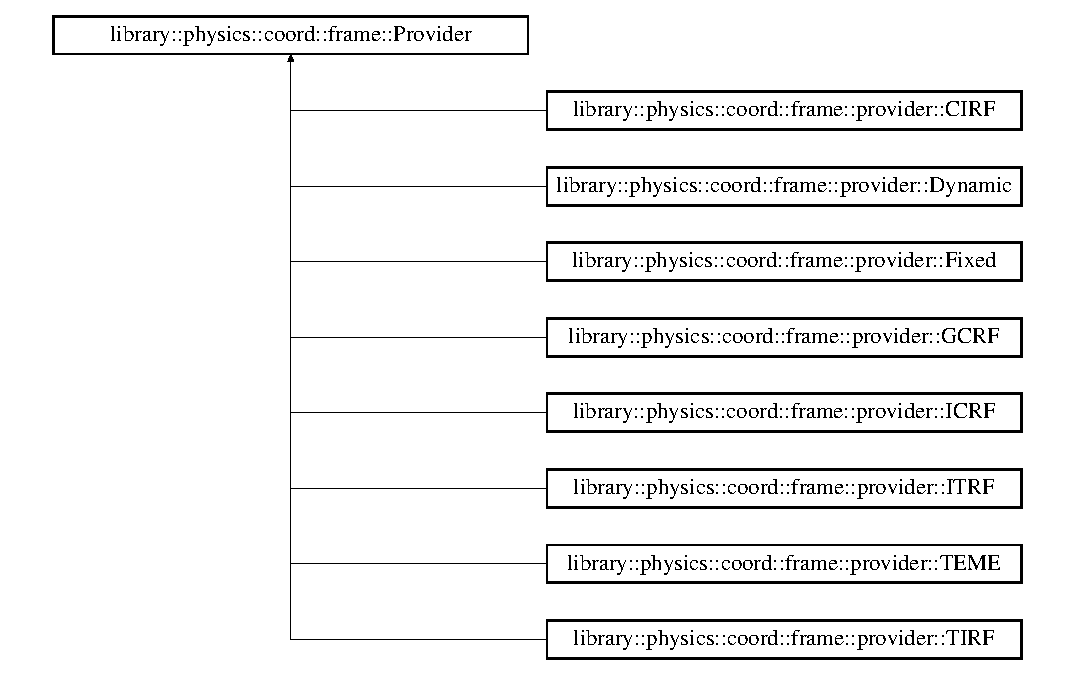
\includegraphics[height=0.577617cm]{classlibrary_1_1physics_1_1coord_1_1frame_1_1_provider}
\end{center}
\end{figure}
\subsection*{Public Member Functions}
\begin{DoxyCompactItemize}
\item 
\hyperlink{classlibrary_1_1physics_1_1coord_1_1frame_1_1_provider_a51327e656332668ba3726d52d7a27f22}{Provider} ()
\item 
virtual \hyperlink{classlibrary_1_1physics_1_1coord_1_1frame_1_1_provider_a7683aa718a339d1bfc8658dc9509adaf}{$\sim$\+Provider} ()=0
\item 
virtual \hyperlink{classlibrary_1_1physics_1_1coord_1_1frame_1_1_provider}{Provider} $\ast$ \hyperlink{classlibrary_1_1physics_1_1coord_1_1frame_1_1_provider_ab8eee40c8ef4aee0b57bedf458f4934e}{clone} () const =0
\item 
virtual bool \hyperlink{classlibrary_1_1physics_1_1coord_1_1frame_1_1_provider_ae7cd093febf2b20f71400f9f79442774}{is\+Defined} () const =0
\item 
virtual \hyperlink{classlibrary_1_1physics_1_1coord_1_1_transform}{Transform} \hyperlink{classlibrary_1_1physics_1_1coord_1_1frame_1_1_provider_a796fd2dd337f1304a0e9acf573ce2550}{get\+Transform\+At} (const \hyperlink{classlibrary_1_1physics_1_1time_1_1_instant}{Instant} \&an\+Instant) const =0
\end{DoxyCompactItemize}


\subsection{Detailed Description}
\hyperlink{classlibrary_1_1physics_1_1coord_1_1_frame}{Frame} provider. 

\subsection{Constructor \& Destructor Documentation}
\mbox{\Hypertarget{classlibrary_1_1physics_1_1coord_1_1frame_1_1_provider_a51327e656332668ba3726d52d7a27f22}\label{classlibrary_1_1physics_1_1coord_1_1frame_1_1_provider_a51327e656332668ba3726d52d7a27f22}} 
\index{library\+::physics\+::coord\+::frame\+::\+Provider@{library\+::physics\+::coord\+::frame\+::\+Provider}!Provider@{Provider}}
\index{Provider@{Provider}!library\+::physics\+::coord\+::frame\+::\+Provider@{library\+::physics\+::coord\+::frame\+::\+Provider}}
\subsubsection{\texorpdfstring{Provider()}{Provider()}}
{\footnotesize\ttfamily library\+::physics\+::coord\+::frame\+::\+Provider\+::\+Provider (\begin{DoxyParamCaption}{ }\end{DoxyParamCaption})}

\mbox{\Hypertarget{classlibrary_1_1physics_1_1coord_1_1frame_1_1_provider_a7683aa718a339d1bfc8658dc9509adaf}\label{classlibrary_1_1physics_1_1coord_1_1frame_1_1_provider_a7683aa718a339d1bfc8658dc9509adaf}} 
\index{library\+::physics\+::coord\+::frame\+::\+Provider@{library\+::physics\+::coord\+::frame\+::\+Provider}!````~Provider@{$\sim$\+Provider}}
\index{````~Provider@{$\sim$\+Provider}!library\+::physics\+::coord\+::frame\+::\+Provider@{library\+::physics\+::coord\+::frame\+::\+Provider}}
\subsubsection{\texorpdfstring{$\sim$\+Provider()}{~Provider()}}
{\footnotesize\ttfamily library\+::physics\+::coord\+::frame\+::\+Provider\+::$\sim$\+Provider (\begin{DoxyParamCaption}{ }\end{DoxyParamCaption})\hspace{0.3cm}{\ttfamily [pure virtual]}}



\subsection{Member Function Documentation}
\mbox{\Hypertarget{classlibrary_1_1physics_1_1coord_1_1frame_1_1_provider_ab8eee40c8ef4aee0b57bedf458f4934e}\label{classlibrary_1_1physics_1_1coord_1_1frame_1_1_provider_ab8eee40c8ef4aee0b57bedf458f4934e}} 
\index{library\+::physics\+::coord\+::frame\+::\+Provider@{library\+::physics\+::coord\+::frame\+::\+Provider}!clone@{clone}}
\index{clone@{clone}!library\+::physics\+::coord\+::frame\+::\+Provider@{library\+::physics\+::coord\+::frame\+::\+Provider}}
\subsubsection{\texorpdfstring{clone()}{clone()}}
{\footnotesize\ttfamily virtual \hyperlink{classlibrary_1_1physics_1_1coord_1_1frame_1_1_provider}{Provider}$\ast$ library\+::physics\+::coord\+::frame\+::\+Provider\+::clone (\begin{DoxyParamCaption}{ }\end{DoxyParamCaption}) const\hspace{0.3cm}{\ttfamily [pure virtual]}}



Implemented in \hyperlink{classlibrary_1_1physics_1_1coord_1_1frame_1_1provider_1_1_c_i_r_f_af75424e9e3a86a5aa06f998a8710c5c2}{library\+::physics\+::coord\+::frame\+::provider\+::\+C\+I\+RF}, \hyperlink{classlibrary_1_1physics_1_1coord_1_1frame_1_1provider_1_1_t_e_m_e_a606d0c4cad7df776e848fd3670e5cc7f}{library\+::physics\+::coord\+::frame\+::provider\+::\+T\+E\+ME}, \hyperlink{classlibrary_1_1physics_1_1coord_1_1frame_1_1provider_1_1_t_i_r_f_a48ef3f686e9bcc744a5e3d1fa1779ab6}{library\+::physics\+::coord\+::frame\+::provider\+::\+T\+I\+RF}, \hyperlink{classlibrary_1_1physics_1_1coord_1_1frame_1_1provider_1_1_g_c_r_f_ae32853b62bfe251fd48262b7ab383fc7}{library\+::physics\+::coord\+::frame\+::provider\+::\+G\+C\+RF}, \hyperlink{classlibrary_1_1physics_1_1coord_1_1frame_1_1provider_1_1_i_c_r_f_a06ce5c7c4bc22045d612d951cbeb4d14}{library\+::physics\+::coord\+::frame\+::provider\+::\+I\+C\+RF}, \hyperlink{classlibrary_1_1physics_1_1coord_1_1frame_1_1provider_1_1_i_t_r_f_a0408f17419e49f785863ba7a84865857}{library\+::physics\+::coord\+::frame\+::provider\+::\+I\+T\+RF}, and \hyperlink{classlibrary_1_1physics_1_1coord_1_1frame_1_1provider_1_1_fixed_aa042b90216dd5276ffca2054c93dfc6e}{library\+::physics\+::coord\+::frame\+::provider\+::\+Fixed}.

\mbox{\Hypertarget{classlibrary_1_1physics_1_1coord_1_1frame_1_1_provider_a796fd2dd337f1304a0e9acf573ce2550}\label{classlibrary_1_1physics_1_1coord_1_1frame_1_1_provider_a796fd2dd337f1304a0e9acf573ce2550}} 
\index{library\+::physics\+::coord\+::frame\+::\+Provider@{library\+::physics\+::coord\+::frame\+::\+Provider}!get\+Transform\+At@{get\+Transform\+At}}
\index{get\+Transform\+At@{get\+Transform\+At}!library\+::physics\+::coord\+::frame\+::\+Provider@{library\+::physics\+::coord\+::frame\+::\+Provider}}
\subsubsection{\texorpdfstring{get\+Transform\+At()}{getTransformAt()}}
{\footnotesize\ttfamily virtual \hyperlink{classlibrary_1_1physics_1_1coord_1_1_transform}{Transform} library\+::physics\+::coord\+::frame\+::\+Provider\+::get\+Transform\+At (\begin{DoxyParamCaption}\item[{const \hyperlink{classlibrary_1_1physics_1_1time_1_1_instant}{Instant} \&}]{an\+Instant }\end{DoxyParamCaption}) const\hspace{0.3cm}{\ttfamily [pure virtual]}}



Implemented in \hyperlink{classlibrary_1_1physics_1_1coord_1_1frame_1_1provider_1_1_c_i_r_f_afa16d0f890856396364443239ceac509}{library\+::physics\+::coord\+::frame\+::provider\+::\+C\+I\+RF}, \hyperlink{classlibrary_1_1physics_1_1coord_1_1frame_1_1provider_1_1_t_e_m_e_a78bd46fa8118d7220ab16a4ca2195299}{library\+::physics\+::coord\+::frame\+::provider\+::\+T\+E\+ME}, \hyperlink{classlibrary_1_1physics_1_1coord_1_1frame_1_1provider_1_1_t_i_r_f_a89eea1b9ff4b38937bf51099e8dd6333}{library\+::physics\+::coord\+::frame\+::provider\+::\+T\+I\+RF}, \hyperlink{classlibrary_1_1physics_1_1coord_1_1frame_1_1provider_1_1_g_c_r_f_a4929dae3032a650b74b77b0d0b9bcaaa}{library\+::physics\+::coord\+::frame\+::provider\+::\+G\+C\+RF}, \hyperlink{classlibrary_1_1physics_1_1coord_1_1frame_1_1provider_1_1_i_c_r_f_a6f5256cac7e8f7b1e947a9f6627a9a33}{library\+::physics\+::coord\+::frame\+::provider\+::\+I\+C\+RF}, \hyperlink{classlibrary_1_1physics_1_1coord_1_1frame_1_1provider_1_1_i_t_r_f_a9fcd6914fa436788b84923a45fe1014e}{library\+::physics\+::coord\+::frame\+::provider\+::\+I\+T\+RF}, and \hyperlink{classlibrary_1_1physics_1_1coord_1_1frame_1_1provider_1_1_fixed_aa5c6299ec0344dbdfb94389b3d7adec5}{library\+::physics\+::coord\+::frame\+::provider\+::\+Fixed}.

\mbox{\Hypertarget{classlibrary_1_1physics_1_1coord_1_1frame_1_1_provider_ae7cd093febf2b20f71400f9f79442774}\label{classlibrary_1_1physics_1_1coord_1_1frame_1_1_provider_ae7cd093febf2b20f71400f9f79442774}} 
\index{library\+::physics\+::coord\+::frame\+::\+Provider@{library\+::physics\+::coord\+::frame\+::\+Provider}!is\+Defined@{is\+Defined}}
\index{is\+Defined@{is\+Defined}!library\+::physics\+::coord\+::frame\+::\+Provider@{library\+::physics\+::coord\+::frame\+::\+Provider}}
\subsubsection{\texorpdfstring{is\+Defined()}{isDefined()}}
{\footnotesize\ttfamily virtual bool library\+::physics\+::coord\+::frame\+::\+Provider\+::is\+Defined (\begin{DoxyParamCaption}{ }\end{DoxyParamCaption}) const\hspace{0.3cm}{\ttfamily [pure virtual]}}



Implemented in \hyperlink{classlibrary_1_1physics_1_1coord_1_1frame_1_1provider_1_1_c_i_r_f_ab5676de1c31ad796d56a684615fabdf8}{library\+::physics\+::coord\+::frame\+::provider\+::\+C\+I\+RF}, \hyperlink{classlibrary_1_1physics_1_1coord_1_1frame_1_1provider_1_1_t_e_m_e_a8c52ea8c59a669197234383e4bfa54b6}{library\+::physics\+::coord\+::frame\+::provider\+::\+T\+E\+ME}, \hyperlink{classlibrary_1_1physics_1_1coord_1_1frame_1_1provider_1_1_t_i_r_f_a3656639fda8a7b991335752559d7594b}{library\+::physics\+::coord\+::frame\+::provider\+::\+T\+I\+RF}, \hyperlink{classlibrary_1_1physics_1_1coord_1_1frame_1_1provider_1_1_g_c_r_f_a0e6155c096ff1c231b14e59544fe038c}{library\+::physics\+::coord\+::frame\+::provider\+::\+G\+C\+RF}, \hyperlink{classlibrary_1_1physics_1_1coord_1_1frame_1_1provider_1_1_i_c_r_f_a533e5d0240150b5c23080ee8bf89d040}{library\+::physics\+::coord\+::frame\+::provider\+::\+I\+C\+RF}, \hyperlink{classlibrary_1_1physics_1_1coord_1_1frame_1_1provider_1_1_i_t_r_f_a10a6a129ab5410f3ad3d687f73ba6d8e}{library\+::physics\+::coord\+::frame\+::provider\+::\+I\+T\+RF}, and \hyperlink{classlibrary_1_1physics_1_1coord_1_1frame_1_1provider_1_1_fixed_ac7a58fa0937c28ed0289c1088275c3d2}{library\+::physics\+::coord\+::frame\+::provider\+::\+Fixed}.



The documentation for this class was generated from the following files\+:\begin{DoxyCompactItemize}
\item 
include/\+Library/\+Physics/\+Coordinate/\+Frame/\hyperlink{_provider_8hpp}{Provider.\+hpp}\item 
src/\+Library/\+Physics/\+Coordinate/\+Frame/\hyperlink{_provider_8cpp}{Provider.\+cpp}\end{DoxyCompactItemize}

\hypertarget{classlibrary_1_1physics_1_1env_1_1ephem_1_1_s_p_i_c_e}{}\section{library\+:\+:physics\+:\+:env\+:\+:ephem\+:\+:S\+P\+I\+CE Class Reference}
\label{classlibrary_1_1physics_1_1env_1_1ephem_1_1_s_p_i_c_e}\index{library\+::physics\+::env\+::ephem\+::\+S\+P\+I\+CE@{library\+::physics\+::env\+::ephem\+::\+S\+P\+I\+CE}}


\hyperlink{classlibrary_1_1physics_1_1env_1_1ephem_1_1_s_p_i_c_e}{S\+P\+I\+CE} Toolkit ephemeris.  




{\ttfamily \#include $<$S\+P\+I\+C\+E.\+hpp$>$}

Inheritance diagram for library\+:\+:physics\+:\+:env\+:\+:ephem\+:\+:S\+P\+I\+CE\+:\begin{figure}[H]
\begin{center}
\leavevmode
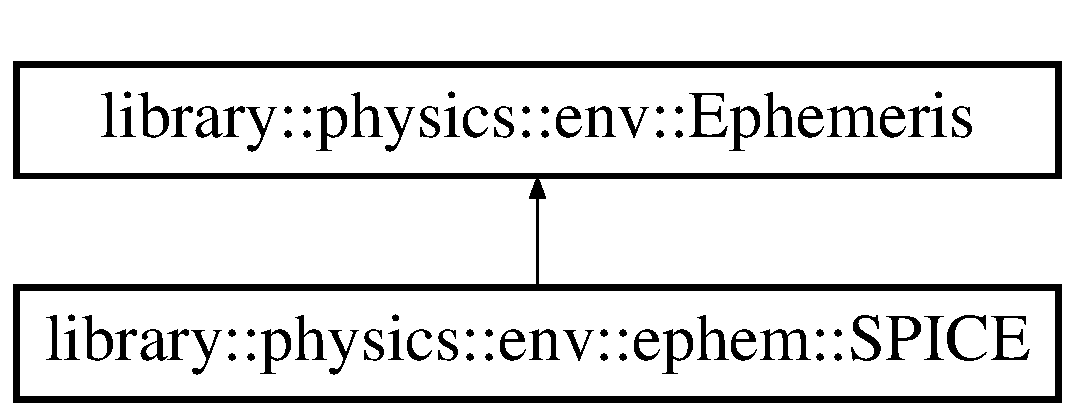
\includegraphics[height=2.000000cm]{classlibrary_1_1physics_1_1env_1_1ephem_1_1_s_p_i_c_e}
\end{center}
\end{figure}
\subsection*{Public Types}
\begin{DoxyCompactItemize}
\item 
enum \hyperlink{classlibrary_1_1physics_1_1env_1_1ephem_1_1_s_p_i_c_e_a86f1a863677210ba8884807cc725c0f8}{Object} \{ \newline
\hyperlink{classlibrary_1_1physics_1_1env_1_1ephem_1_1_s_p_i_c_e_a86f1a863677210ba8884807cc725c0f8aef6572e4cd58bb39a3f4e82fc64fe9f0}{Object\+::\+Sun}, 
\hyperlink{classlibrary_1_1physics_1_1env_1_1ephem_1_1_s_p_i_c_e_a86f1a863677210ba8884807cc725c0f8a34dae487e31f37aa74633258b7774d4f}{Object\+::\+Mercury}, 
\hyperlink{classlibrary_1_1physics_1_1env_1_1ephem_1_1_s_p_i_c_e_a86f1a863677210ba8884807cc725c0f8a0bdc508a17811a3a860d32749ad44e4b}{Object\+::\+Venus}, 
\hyperlink{classlibrary_1_1physics_1_1env_1_1ephem_1_1_s_p_i_c_e_a86f1a863677210ba8884807cc725c0f8a5cdd21c97f86686cc505e02fd32a7523}{Object\+::\+Earth}, 
\newline
\hyperlink{classlibrary_1_1physics_1_1env_1_1ephem_1_1_s_p_i_c_e_a86f1a863677210ba8884807cc725c0f8ad502a50ed945d5fca74e0105575b5b34}{Object\+::\+Moon}, 
\hyperlink{classlibrary_1_1physics_1_1env_1_1ephem_1_1_s_p_i_c_e_a86f1a863677210ba8884807cc725c0f8a671f028142280b556a85ffdd90e0a43d}{Object\+::\+Mars}, 
\hyperlink{classlibrary_1_1physics_1_1env_1_1ephem_1_1_s_p_i_c_e_a86f1a863677210ba8884807cc725c0f8a89c5c30498c2989611f9044be006197c}{Object\+::\+Jupiter}, 
\hyperlink{classlibrary_1_1physics_1_1env_1_1ephem_1_1_s_p_i_c_e_a86f1a863677210ba8884807cc725c0f8a233ea1805dab5120a0ecc49b71a48063}{Object\+::\+Saturn}, 
\newline
\hyperlink{classlibrary_1_1physics_1_1env_1_1ephem_1_1_s_p_i_c_e_a86f1a863677210ba8884807cc725c0f8a76b840d32f33267ad812507b47e3a1b5}{Object\+::\+Uranus}, 
\hyperlink{classlibrary_1_1physics_1_1env_1_1ephem_1_1_s_p_i_c_e_a86f1a863677210ba8884807cc725c0f8af8d3b65d8479a31ebf67cb18dd0a4641}{Object\+::\+Neptune}
 \}
\end{DoxyCompactItemize}
\subsection*{Public Member Functions}
\begin{DoxyCompactItemize}
\item 
\hyperlink{classlibrary_1_1physics_1_1env_1_1ephem_1_1_s_p_i_c_e_a736d504ac455e1c1ccadd03f11611e4b}{S\+P\+I\+CE} (const \hyperlink{classlibrary_1_1physics_1_1env_1_1ephem_1_1_s_p_i_c_e_a86f1a863677210ba8884807cc725c0f8}{S\+P\+I\+C\+E\+::\+Object} \&an\+Object)
\item 
virtual \hyperlink{classlibrary_1_1physics_1_1env_1_1ephem_1_1_s_p_i_c_e_ae6f089a215f400957d5cad057997d007}{$\sim$\+S\+P\+I\+CE} () override
\item 
virtual \hyperlink{classlibrary_1_1physics_1_1env_1_1ephem_1_1_s_p_i_c_e}{S\+P\+I\+CE} $\ast$ \hyperlink{classlibrary_1_1physics_1_1env_1_1ephem_1_1_s_p_i_c_e_a7d397f5472ec2e14d85fa493cb7c9ae0}{clone} () const override
\item 
virtual bool \hyperlink{classlibrary_1_1physics_1_1env_1_1ephem_1_1_s_p_i_c_e_a54fb3fb8768a72f515231dac083eb9cb}{is\+Defined} () const override
\item 
virtual Shared$<$ const \hyperlink{classlibrary_1_1physics_1_1coord_1_1_frame}{Frame} $>$ \hyperlink{classlibrary_1_1physics_1_1env_1_1ephem_1_1_s_p_i_c_e_a20b94d4f05b17a2eb3ba986464da44a8}{access\+Frame} () const override
\end{DoxyCompactItemize}
\subsection*{Static Public Member Functions}
\begin{DoxyCompactItemize}
\item 
static String \hyperlink{classlibrary_1_1physics_1_1env_1_1ephem_1_1_s_p_i_c_e_aebeefe1b806d93e576a0b08c8d24b250}{String\+From\+Object} (const \hyperlink{classlibrary_1_1physics_1_1env_1_1ephem_1_1_s_p_i_c_e_a86f1a863677210ba8884807cc725c0f8}{S\+P\+I\+C\+E\+::\+Object} \&an\+Object)
\end{DoxyCompactItemize}


\subsection{Detailed Description}
\hyperlink{classlibrary_1_1physics_1_1env_1_1ephem_1_1_s_p_i_c_e}{S\+P\+I\+CE} Toolkit ephemeris. 

https\+://en.wikipedia.\+org/wiki/\+Jet\+\_\+\+Propulsion\+\_\+\+Laboratory\+\_\+\+Development\+\_\+\+Ephemeris 

\subsection{Member Enumeration Documentation}
\mbox{\Hypertarget{classlibrary_1_1physics_1_1env_1_1ephem_1_1_s_p_i_c_e_a86f1a863677210ba8884807cc725c0f8}\label{classlibrary_1_1physics_1_1env_1_1ephem_1_1_s_p_i_c_e_a86f1a863677210ba8884807cc725c0f8}} 
\index{library\+::physics\+::env\+::ephem\+::\+S\+P\+I\+CE@{library\+::physics\+::env\+::ephem\+::\+S\+P\+I\+CE}!Object@{Object}}
\index{Object@{Object}!library\+::physics\+::env\+::ephem\+::\+S\+P\+I\+CE@{library\+::physics\+::env\+::ephem\+::\+S\+P\+I\+CE}}
\subsubsection{\texorpdfstring{Object}{Object}}
{\footnotesize\ttfamily enum \hyperlink{classlibrary_1_1physics_1_1env_1_1ephem_1_1_s_p_i_c_e_a86f1a863677210ba8884807cc725c0f8}{library\+::physics\+::env\+::ephem\+::\+S\+P\+I\+C\+E\+::\+Object}\hspace{0.3cm}{\ttfamily [strong]}}

\begin{DoxyEnumFields}{Enumerator}
\raisebox{\heightof{T}}[0pt][0pt]{\index{Sun@{Sun}!library\+::physics\+::env\+::ephem\+::\+S\+P\+I\+CE@{library\+::physics\+::env\+::ephem\+::\+S\+P\+I\+CE}}\index{library\+::physics\+::env\+::ephem\+::\+S\+P\+I\+CE@{library\+::physics\+::env\+::ephem\+::\+S\+P\+I\+CE}!Sun@{Sun}}}\mbox{\Hypertarget{classlibrary_1_1physics_1_1env_1_1ephem_1_1_s_p_i_c_e_a86f1a863677210ba8884807cc725c0f8aef6572e4cd58bb39a3f4e82fc64fe9f0}\label{classlibrary_1_1physics_1_1env_1_1ephem_1_1_s_p_i_c_e_a86f1a863677210ba8884807cc725c0f8aef6572e4cd58bb39a3f4e82fc64fe9f0}} 
Sun&\\
\hline

\raisebox{\heightof{T}}[0pt][0pt]{\index{Mercury@{Mercury}!library\+::physics\+::env\+::ephem\+::\+S\+P\+I\+CE@{library\+::physics\+::env\+::ephem\+::\+S\+P\+I\+CE}}\index{library\+::physics\+::env\+::ephem\+::\+S\+P\+I\+CE@{library\+::physics\+::env\+::ephem\+::\+S\+P\+I\+CE}!Mercury@{Mercury}}}\mbox{\Hypertarget{classlibrary_1_1physics_1_1env_1_1ephem_1_1_s_p_i_c_e_a86f1a863677210ba8884807cc725c0f8a34dae487e31f37aa74633258b7774d4f}\label{classlibrary_1_1physics_1_1env_1_1ephem_1_1_s_p_i_c_e_a86f1a863677210ba8884807cc725c0f8a34dae487e31f37aa74633258b7774d4f}} 
Mercury&\\
\hline

\raisebox{\heightof{T}}[0pt][0pt]{\index{Venus@{Venus}!library\+::physics\+::env\+::ephem\+::\+S\+P\+I\+CE@{library\+::physics\+::env\+::ephem\+::\+S\+P\+I\+CE}}\index{library\+::physics\+::env\+::ephem\+::\+S\+P\+I\+CE@{library\+::physics\+::env\+::ephem\+::\+S\+P\+I\+CE}!Venus@{Venus}}}\mbox{\Hypertarget{classlibrary_1_1physics_1_1env_1_1ephem_1_1_s_p_i_c_e_a86f1a863677210ba8884807cc725c0f8a0bdc508a17811a3a860d32749ad44e4b}\label{classlibrary_1_1physics_1_1env_1_1ephem_1_1_s_p_i_c_e_a86f1a863677210ba8884807cc725c0f8a0bdc508a17811a3a860d32749ad44e4b}} 
Venus&\\
\hline

\raisebox{\heightof{T}}[0pt][0pt]{\index{Earth@{Earth}!library\+::physics\+::env\+::ephem\+::\+S\+P\+I\+CE@{library\+::physics\+::env\+::ephem\+::\+S\+P\+I\+CE}}\index{library\+::physics\+::env\+::ephem\+::\+S\+P\+I\+CE@{library\+::physics\+::env\+::ephem\+::\+S\+P\+I\+CE}!Earth@{Earth}}}\mbox{\Hypertarget{classlibrary_1_1physics_1_1env_1_1ephem_1_1_s_p_i_c_e_a86f1a863677210ba8884807cc725c0f8a5cdd21c97f86686cc505e02fd32a7523}\label{classlibrary_1_1physics_1_1env_1_1ephem_1_1_s_p_i_c_e_a86f1a863677210ba8884807cc725c0f8a5cdd21c97f86686cc505e02fd32a7523}} 
Earth&\\
\hline

\raisebox{\heightof{T}}[0pt][0pt]{\index{Moon@{Moon}!library\+::physics\+::env\+::ephem\+::\+S\+P\+I\+CE@{library\+::physics\+::env\+::ephem\+::\+S\+P\+I\+CE}}\index{library\+::physics\+::env\+::ephem\+::\+S\+P\+I\+CE@{library\+::physics\+::env\+::ephem\+::\+S\+P\+I\+CE}!Moon@{Moon}}}\mbox{\Hypertarget{classlibrary_1_1physics_1_1env_1_1ephem_1_1_s_p_i_c_e_a86f1a863677210ba8884807cc725c0f8ad502a50ed945d5fca74e0105575b5b34}\label{classlibrary_1_1physics_1_1env_1_1ephem_1_1_s_p_i_c_e_a86f1a863677210ba8884807cc725c0f8ad502a50ed945d5fca74e0105575b5b34}} 
Moon&\\
\hline

\raisebox{\heightof{T}}[0pt][0pt]{\index{Mars@{Mars}!library\+::physics\+::env\+::ephem\+::\+S\+P\+I\+CE@{library\+::physics\+::env\+::ephem\+::\+S\+P\+I\+CE}}\index{library\+::physics\+::env\+::ephem\+::\+S\+P\+I\+CE@{library\+::physics\+::env\+::ephem\+::\+S\+P\+I\+CE}!Mars@{Mars}}}\mbox{\Hypertarget{classlibrary_1_1physics_1_1env_1_1ephem_1_1_s_p_i_c_e_a86f1a863677210ba8884807cc725c0f8a671f028142280b556a85ffdd90e0a43d}\label{classlibrary_1_1physics_1_1env_1_1ephem_1_1_s_p_i_c_e_a86f1a863677210ba8884807cc725c0f8a671f028142280b556a85ffdd90e0a43d}} 
Mars&\\
\hline

\raisebox{\heightof{T}}[0pt][0pt]{\index{Jupiter@{Jupiter}!library\+::physics\+::env\+::ephem\+::\+S\+P\+I\+CE@{library\+::physics\+::env\+::ephem\+::\+S\+P\+I\+CE}}\index{library\+::physics\+::env\+::ephem\+::\+S\+P\+I\+CE@{library\+::physics\+::env\+::ephem\+::\+S\+P\+I\+CE}!Jupiter@{Jupiter}}}\mbox{\Hypertarget{classlibrary_1_1physics_1_1env_1_1ephem_1_1_s_p_i_c_e_a86f1a863677210ba8884807cc725c0f8a89c5c30498c2989611f9044be006197c}\label{classlibrary_1_1physics_1_1env_1_1ephem_1_1_s_p_i_c_e_a86f1a863677210ba8884807cc725c0f8a89c5c30498c2989611f9044be006197c}} 
Jupiter&\\
\hline

\raisebox{\heightof{T}}[0pt][0pt]{\index{Saturn@{Saturn}!library\+::physics\+::env\+::ephem\+::\+S\+P\+I\+CE@{library\+::physics\+::env\+::ephem\+::\+S\+P\+I\+CE}}\index{library\+::physics\+::env\+::ephem\+::\+S\+P\+I\+CE@{library\+::physics\+::env\+::ephem\+::\+S\+P\+I\+CE}!Saturn@{Saturn}}}\mbox{\Hypertarget{classlibrary_1_1physics_1_1env_1_1ephem_1_1_s_p_i_c_e_a86f1a863677210ba8884807cc725c0f8a233ea1805dab5120a0ecc49b71a48063}\label{classlibrary_1_1physics_1_1env_1_1ephem_1_1_s_p_i_c_e_a86f1a863677210ba8884807cc725c0f8a233ea1805dab5120a0ecc49b71a48063}} 
Saturn&\\
\hline

\raisebox{\heightof{T}}[0pt][0pt]{\index{Uranus@{Uranus}!library\+::physics\+::env\+::ephem\+::\+S\+P\+I\+CE@{library\+::physics\+::env\+::ephem\+::\+S\+P\+I\+CE}}\index{library\+::physics\+::env\+::ephem\+::\+S\+P\+I\+CE@{library\+::physics\+::env\+::ephem\+::\+S\+P\+I\+CE}!Uranus@{Uranus}}}\mbox{\Hypertarget{classlibrary_1_1physics_1_1env_1_1ephem_1_1_s_p_i_c_e_a86f1a863677210ba8884807cc725c0f8a76b840d32f33267ad812507b47e3a1b5}\label{classlibrary_1_1physics_1_1env_1_1ephem_1_1_s_p_i_c_e_a86f1a863677210ba8884807cc725c0f8a76b840d32f33267ad812507b47e3a1b5}} 
Uranus&\\
\hline

\raisebox{\heightof{T}}[0pt][0pt]{\index{Neptune@{Neptune}!library\+::physics\+::env\+::ephem\+::\+S\+P\+I\+CE@{library\+::physics\+::env\+::ephem\+::\+S\+P\+I\+CE}}\index{library\+::physics\+::env\+::ephem\+::\+S\+P\+I\+CE@{library\+::physics\+::env\+::ephem\+::\+S\+P\+I\+CE}!Neptune@{Neptune}}}\mbox{\Hypertarget{classlibrary_1_1physics_1_1env_1_1ephem_1_1_s_p_i_c_e_a86f1a863677210ba8884807cc725c0f8af8d3b65d8479a31ebf67cb18dd0a4641}\label{classlibrary_1_1physics_1_1env_1_1ephem_1_1_s_p_i_c_e_a86f1a863677210ba8884807cc725c0f8af8d3b65d8479a31ebf67cb18dd0a4641}} 
Neptune&\\
\hline

\end{DoxyEnumFields}


\subsection{Constructor \& Destructor Documentation}
\mbox{\Hypertarget{classlibrary_1_1physics_1_1env_1_1ephem_1_1_s_p_i_c_e_a736d504ac455e1c1ccadd03f11611e4b}\label{classlibrary_1_1physics_1_1env_1_1ephem_1_1_s_p_i_c_e_a736d504ac455e1c1ccadd03f11611e4b}} 
\index{library\+::physics\+::env\+::ephem\+::\+S\+P\+I\+CE@{library\+::physics\+::env\+::ephem\+::\+S\+P\+I\+CE}!S\+P\+I\+CE@{S\+P\+I\+CE}}
\index{S\+P\+I\+CE@{S\+P\+I\+CE}!library\+::physics\+::env\+::ephem\+::\+S\+P\+I\+CE@{library\+::physics\+::env\+::ephem\+::\+S\+P\+I\+CE}}
\subsubsection{\texorpdfstring{S\+P\+I\+C\+E()}{SPICE()}}
{\footnotesize\ttfamily library\+::physics\+::env\+::ephem\+::\+S\+P\+I\+C\+E\+::\+S\+P\+I\+CE (\begin{DoxyParamCaption}\item[{const \hyperlink{classlibrary_1_1physics_1_1env_1_1ephem_1_1_s_p_i_c_e_a86f1a863677210ba8884807cc725c0f8}{S\+P\+I\+C\+E\+::\+Object} \&}]{an\+Object }\end{DoxyParamCaption})}

\mbox{\Hypertarget{classlibrary_1_1physics_1_1env_1_1ephem_1_1_s_p_i_c_e_ae6f089a215f400957d5cad057997d007}\label{classlibrary_1_1physics_1_1env_1_1ephem_1_1_s_p_i_c_e_ae6f089a215f400957d5cad057997d007}} 
\index{library\+::physics\+::env\+::ephem\+::\+S\+P\+I\+CE@{library\+::physics\+::env\+::ephem\+::\+S\+P\+I\+CE}!````~S\+P\+I\+CE@{$\sim$\+S\+P\+I\+CE}}
\index{````~S\+P\+I\+CE@{$\sim$\+S\+P\+I\+CE}!library\+::physics\+::env\+::ephem\+::\+S\+P\+I\+CE@{library\+::physics\+::env\+::ephem\+::\+S\+P\+I\+CE}}
\subsubsection{\texorpdfstring{$\sim$\+S\+P\+I\+C\+E()}{~SPICE()}}
{\footnotesize\ttfamily library\+::physics\+::env\+::ephem\+::\+S\+P\+I\+C\+E\+::$\sim$\+S\+P\+I\+CE (\begin{DoxyParamCaption}{ }\end{DoxyParamCaption})\hspace{0.3cm}{\ttfamily [override]}, {\ttfamily [virtual]}}



\subsection{Member Function Documentation}
\mbox{\Hypertarget{classlibrary_1_1physics_1_1env_1_1ephem_1_1_s_p_i_c_e_a20b94d4f05b17a2eb3ba986464da44a8}\label{classlibrary_1_1physics_1_1env_1_1ephem_1_1_s_p_i_c_e_a20b94d4f05b17a2eb3ba986464da44a8}} 
\index{library\+::physics\+::env\+::ephem\+::\+S\+P\+I\+CE@{library\+::physics\+::env\+::ephem\+::\+S\+P\+I\+CE}!access\+Frame@{access\+Frame}}
\index{access\+Frame@{access\+Frame}!library\+::physics\+::env\+::ephem\+::\+S\+P\+I\+CE@{library\+::physics\+::env\+::ephem\+::\+S\+P\+I\+CE}}
\subsubsection{\texorpdfstring{access\+Frame()}{accessFrame()}}
{\footnotesize\ttfamily Shared$<$ const \hyperlink{classlibrary_1_1physics_1_1coord_1_1_frame}{Frame} $>$ library\+::physics\+::env\+::ephem\+::\+S\+P\+I\+C\+E\+::access\+Frame (\begin{DoxyParamCaption}{ }\end{DoxyParamCaption}) const\hspace{0.3cm}{\ttfamily [override]}, {\ttfamily [virtual]}}



Implements \hyperlink{classlibrary_1_1physics_1_1env_1_1_ephemeris_ac832f493239ace4d53c1c5130c1dad31}{library\+::physics\+::env\+::\+Ephemeris}.

\mbox{\Hypertarget{classlibrary_1_1physics_1_1env_1_1ephem_1_1_s_p_i_c_e_a7d397f5472ec2e14d85fa493cb7c9ae0}\label{classlibrary_1_1physics_1_1env_1_1ephem_1_1_s_p_i_c_e_a7d397f5472ec2e14d85fa493cb7c9ae0}} 
\index{library\+::physics\+::env\+::ephem\+::\+S\+P\+I\+CE@{library\+::physics\+::env\+::ephem\+::\+S\+P\+I\+CE}!clone@{clone}}
\index{clone@{clone}!library\+::physics\+::env\+::ephem\+::\+S\+P\+I\+CE@{library\+::physics\+::env\+::ephem\+::\+S\+P\+I\+CE}}
\subsubsection{\texorpdfstring{clone()}{clone()}}
{\footnotesize\ttfamily \hyperlink{classlibrary_1_1physics_1_1env_1_1ephem_1_1_s_p_i_c_e}{S\+P\+I\+CE} $\ast$ library\+::physics\+::env\+::ephem\+::\+S\+P\+I\+C\+E\+::clone (\begin{DoxyParamCaption}{ }\end{DoxyParamCaption}) const\hspace{0.3cm}{\ttfamily [override]}, {\ttfamily [virtual]}}



Implements \hyperlink{classlibrary_1_1physics_1_1env_1_1_ephemeris_a7ddecd88d91f79ff204100eb9607b591}{library\+::physics\+::env\+::\+Ephemeris}.

\mbox{\Hypertarget{classlibrary_1_1physics_1_1env_1_1ephem_1_1_s_p_i_c_e_a54fb3fb8768a72f515231dac083eb9cb}\label{classlibrary_1_1physics_1_1env_1_1ephem_1_1_s_p_i_c_e_a54fb3fb8768a72f515231dac083eb9cb}} 
\index{library\+::physics\+::env\+::ephem\+::\+S\+P\+I\+CE@{library\+::physics\+::env\+::ephem\+::\+S\+P\+I\+CE}!is\+Defined@{is\+Defined}}
\index{is\+Defined@{is\+Defined}!library\+::physics\+::env\+::ephem\+::\+S\+P\+I\+CE@{library\+::physics\+::env\+::ephem\+::\+S\+P\+I\+CE}}
\subsubsection{\texorpdfstring{is\+Defined()}{isDefined()}}
{\footnotesize\ttfamily bool library\+::physics\+::env\+::ephem\+::\+S\+P\+I\+C\+E\+::is\+Defined (\begin{DoxyParamCaption}{ }\end{DoxyParamCaption}) const\hspace{0.3cm}{\ttfamily [override]}, {\ttfamily [virtual]}}



Implements \hyperlink{classlibrary_1_1physics_1_1env_1_1_ephemeris_abf61a03e24dd146199381db14d1d7c68}{library\+::physics\+::env\+::\+Ephemeris}.

\mbox{\Hypertarget{classlibrary_1_1physics_1_1env_1_1ephem_1_1_s_p_i_c_e_aebeefe1b806d93e576a0b08c8d24b250}\label{classlibrary_1_1physics_1_1env_1_1ephem_1_1_s_p_i_c_e_aebeefe1b806d93e576a0b08c8d24b250}} 
\index{library\+::physics\+::env\+::ephem\+::\+S\+P\+I\+CE@{library\+::physics\+::env\+::ephem\+::\+S\+P\+I\+CE}!String\+From\+Object@{String\+From\+Object}}
\index{String\+From\+Object@{String\+From\+Object}!library\+::physics\+::env\+::ephem\+::\+S\+P\+I\+CE@{library\+::physics\+::env\+::ephem\+::\+S\+P\+I\+CE}}
\subsubsection{\texorpdfstring{String\+From\+Object()}{StringFromObject()}}
{\footnotesize\ttfamily String library\+::physics\+::env\+::ephem\+::\+S\+P\+I\+C\+E\+::\+String\+From\+Object (\begin{DoxyParamCaption}\item[{const \hyperlink{classlibrary_1_1physics_1_1env_1_1ephem_1_1_s_p_i_c_e_a86f1a863677210ba8884807cc725c0f8}{S\+P\+I\+C\+E\+::\+Object} \&}]{an\+Object }\end{DoxyParamCaption})\hspace{0.3cm}{\ttfamily [static]}}



The documentation for this class was generated from the following files\+:\begin{DoxyCompactItemize}
\item 
include/\+Library/\+Physics/\+Environment/\+Ephemerides/\hyperlink{_s_p_i_c_e_8hpp}{S\+P\+I\+C\+E.\+hpp}\item 
src/\+Library/\+Physics/\+Environment/\+Ephemerides/\hyperlink{_s_p_i_c_e_8cpp}{S\+P\+I\+C\+E.\+cpp}\end{DoxyCompactItemize}

\hypertarget{classlibrary_1_1physics_1_1coord_1_1frame_1_1provider_1_1_static}{}\section{library\+:\+:physics\+:\+:coord\+:\+:frame\+:\+:provider\+:\+:Static Class Reference}
\label{classlibrary_1_1physics_1_1coord_1_1frame_1_1provider_1_1_static}\index{library\+::physics\+::coord\+::frame\+::provider\+::\+Static@{library\+::physics\+::coord\+::frame\+::provider\+::\+Static}}


\hyperlink{classlibrary_1_1physics_1_1coord_1_1frame_1_1provider_1_1_static}{Static} provider.  




{\ttfamily \#include $<$Static.\+hpp$>$}

Inheritance diagram for library\+:\+:physics\+:\+:coord\+:\+:frame\+:\+:provider\+:\+:Static\+:\begin{figure}[H]
\begin{center}
\leavevmode
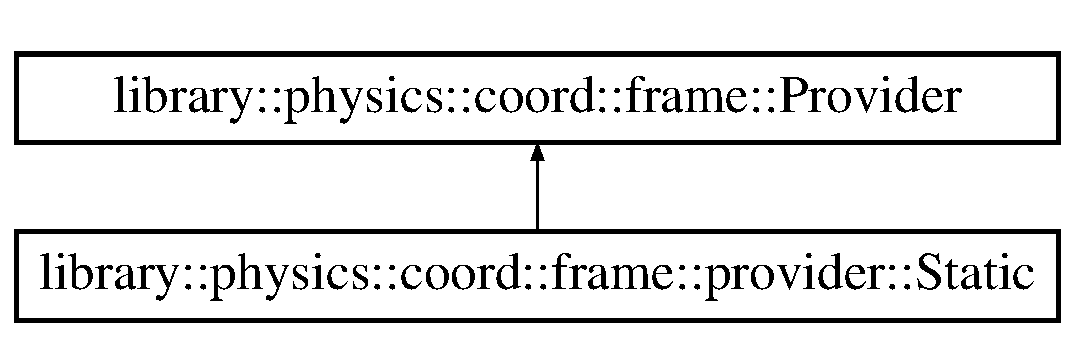
\includegraphics[height=2.000000cm]{classlibrary_1_1physics_1_1coord_1_1frame_1_1provider_1_1_static}
\end{center}
\end{figure}
\subsection*{Public Member Functions}
\begin{DoxyCompactItemize}
\item 
\hyperlink{classlibrary_1_1physics_1_1coord_1_1frame_1_1provider_1_1_static_a2cc2ad821e2c251fe505439551b634fc}{Static} (const \hyperlink{classlibrary_1_1physics_1_1coord_1_1_transform}{Transform} \&a\+Transform)
\item 
virtual \hyperlink{classlibrary_1_1physics_1_1coord_1_1frame_1_1provider_1_1_static_ac2eedd75deffe49efa2de7ccf22f4a4a}{$\sim$\+Static} () override
\item 
virtual \hyperlink{classlibrary_1_1physics_1_1coord_1_1frame_1_1provider_1_1_static}{Static} $\ast$ \hyperlink{classlibrary_1_1physics_1_1coord_1_1frame_1_1provider_1_1_static_aa9062e601039a575302ea34e87e4dedc}{clone} () const override
\item 
virtual bool \hyperlink{classlibrary_1_1physics_1_1coord_1_1frame_1_1provider_1_1_static_a508f20f859dbc43759ab64e03b5befa1}{is\+Defined} () const override
\item 
virtual \hyperlink{classlibrary_1_1physics_1_1coord_1_1_transform}{Transform} \hyperlink{classlibrary_1_1physics_1_1coord_1_1frame_1_1provider_1_1_static_a0999bb357a22d2e626aeaae81031fd46}{get\+Transform\+At} (const \hyperlink{classlibrary_1_1physics_1_1time_1_1_instant}{Instant} \&an\+Instant) const override
\end{DoxyCompactItemize}


\subsection{Detailed Description}
\hyperlink{classlibrary_1_1physics_1_1coord_1_1frame_1_1provider_1_1_static}{Static} provider. 

\subsection{Constructor \& Destructor Documentation}
\mbox{\Hypertarget{classlibrary_1_1physics_1_1coord_1_1frame_1_1provider_1_1_static_a2cc2ad821e2c251fe505439551b634fc}\label{classlibrary_1_1physics_1_1coord_1_1frame_1_1provider_1_1_static_a2cc2ad821e2c251fe505439551b634fc}} 
\index{library\+::physics\+::coord\+::frame\+::provider\+::\+Static@{library\+::physics\+::coord\+::frame\+::provider\+::\+Static}!Static@{Static}}
\index{Static@{Static}!library\+::physics\+::coord\+::frame\+::provider\+::\+Static@{library\+::physics\+::coord\+::frame\+::provider\+::\+Static}}
\subsubsection{\texorpdfstring{Static()}{Static()}}
{\footnotesize\ttfamily library\+::physics\+::coord\+::frame\+::provider\+::\+Static\+::\+Static (\begin{DoxyParamCaption}\item[{const \hyperlink{classlibrary_1_1physics_1_1coord_1_1_transform}{Transform} \&}]{a\+Transform }\end{DoxyParamCaption})}

\mbox{\Hypertarget{classlibrary_1_1physics_1_1coord_1_1frame_1_1provider_1_1_static_ac2eedd75deffe49efa2de7ccf22f4a4a}\label{classlibrary_1_1physics_1_1coord_1_1frame_1_1provider_1_1_static_ac2eedd75deffe49efa2de7ccf22f4a4a}} 
\index{library\+::physics\+::coord\+::frame\+::provider\+::\+Static@{library\+::physics\+::coord\+::frame\+::provider\+::\+Static}!````~Static@{$\sim$\+Static}}
\index{````~Static@{$\sim$\+Static}!library\+::physics\+::coord\+::frame\+::provider\+::\+Static@{library\+::physics\+::coord\+::frame\+::provider\+::\+Static}}
\subsubsection{\texorpdfstring{$\sim$\+Static()}{~Static()}}
{\footnotesize\ttfamily library\+::physics\+::coord\+::frame\+::provider\+::\+Static\+::$\sim$\+Static (\begin{DoxyParamCaption}{ }\end{DoxyParamCaption})\hspace{0.3cm}{\ttfamily [override]}, {\ttfamily [virtual]}}



\subsection{Member Function Documentation}
\mbox{\Hypertarget{classlibrary_1_1physics_1_1coord_1_1frame_1_1provider_1_1_static_aa9062e601039a575302ea34e87e4dedc}\label{classlibrary_1_1physics_1_1coord_1_1frame_1_1provider_1_1_static_aa9062e601039a575302ea34e87e4dedc}} 
\index{library\+::physics\+::coord\+::frame\+::provider\+::\+Static@{library\+::physics\+::coord\+::frame\+::provider\+::\+Static}!clone@{clone}}
\index{clone@{clone}!library\+::physics\+::coord\+::frame\+::provider\+::\+Static@{library\+::physics\+::coord\+::frame\+::provider\+::\+Static}}
\subsubsection{\texorpdfstring{clone()}{clone()}}
{\footnotesize\ttfamily \hyperlink{classlibrary_1_1physics_1_1coord_1_1frame_1_1provider_1_1_static}{Static} $\ast$ library\+::physics\+::coord\+::frame\+::provider\+::\+Static\+::clone (\begin{DoxyParamCaption}{ }\end{DoxyParamCaption}) const\hspace{0.3cm}{\ttfamily [override]}, {\ttfamily [virtual]}}



Implements \hyperlink{classlibrary_1_1physics_1_1coord_1_1frame_1_1_provider_ab8eee40c8ef4aee0b57bedf458f4934e}{library\+::physics\+::coord\+::frame\+::\+Provider}.

\mbox{\Hypertarget{classlibrary_1_1physics_1_1coord_1_1frame_1_1provider_1_1_static_a0999bb357a22d2e626aeaae81031fd46}\label{classlibrary_1_1physics_1_1coord_1_1frame_1_1provider_1_1_static_a0999bb357a22d2e626aeaae81031fd46}} 
\index{library\+::physics\+::coord\+::frame\+::provider\+::\+Static@{library\+::physics\+::coord\+::frame\+::provider\+::\+Static}!get\+Transform\+At@{get\+Transform\+At}}
\index{get\+Transform\+At@{get\+Transform\+At}!library\+::physics\+::coord\+::frame\+::provider\+::\+Static@{library\+::physics\+::coord\+::frame\+::provider\+::\+Static}}
\subsubsection{\texorpdfstring{get\+Transform\+At()}{getTransformAt()}}
{\footnotesize\ttfamily \hyperlink{classlibrary_1_1physics_1_1coord_1_1_transform}{Transform} library\+::physics\+::coord\+::frame\+::provider\+::\+Static\+::get\+Transform\+At (\begin{DoxyParamCaption}\item[{const \hyperlink{classlibrary_1_1physics_1_1time_1_1_instant}{Instant} \&}]{an\+Instant }\end{DoxyParamCaption}) const\hspace{0.3cm}{\ttfamily [override]}, {\ttfamily [virtual]}}



Implements \hyperlink{classlibrary_1_1physics_1_1coord_1_1frame_1_1_provider_a796fd2dd337f1304a0e9acf573ce2550}{library\+::physics\+::coord\+::frame\+::\+Provider}.

\mbox{\Hypertarget{classlibrary_1_1physics_1_1coord_1_1frame_1_1provider_1_1_static_a508f20f859dbc43759ab64e03b5befa1}\label{classlibrary_1_1physics_1_1coord_1_1frame_1_1provider_1_1_static_a508f20f859dbc43759ab64e03b5befa1}} 
\index{library\+::physics\+::coord\+::frame\+::provider\+::\+Static@{library\+::physics\+::coord\+::frame\+::provider\+::\+Static}!is\+Defined@{is\+Defined}}
\index{is\+Defined@{is\+Defined}!library\+::physics\+::coord\+::frame\+::provider\+::\+Static@{library\+::physics\+::coord\+::frame\+::provider\+::\+Static}}
\subsubsection{\texorpdfstring{is\+Defined()}{isDefined()}}
{\footnotesize\ttfamily bool library\+::physics\+::coord\+::frame\+::provider\+::\+Static\+::is\+Defined (\begin{DoxyParamCaption}{ }\end{DoxyParamCaption}) const\hspace{0.3cm}{\ttfamily [override]}, {\ttfamily [virtual]}}



Implements \hyperlink{classlibrary_1_1physics_1_1coord_1_1frame_1_1_provider_ae7cd093febf2b20f71400f9f79442774}{library\+::physics\+::coord\+::frame\+::\+Provider}.



The documentation for this class was generated from the following files\+:\begin{DoxyCompactItemize}
\item 
include/\+Library/\+Physics/\+Coordinate/\+Frame/\+Providers/\hyperlink{_static_8hpp}{Static.\+hpp}\item 
src/\+Library/\+Physics/\+Coordinate/\+Frame/\+Providers/\hyperlink{_static_8cpp}{Static.\+cpp}\end{DoxyCompactItemize}

\hypertarget{classlibrary_1_1physics_1_1env_1_1obj_1_1celest_1_1_sun}{}\section{library\+:\+:physics\+:\+:env\+:\+:obj\+:\+:celest\+:\+:Sun Class Reference}
\label{classlibrary_1_1physics_1_1env_1_1obj_1_1celest_1_1_sun}\index{library\+::physics\+::env\+::obj\+::celest\+::\+Sun@{library\+::physics\+::env\+::obj\+::celest\+::\+Sun}}


{\ttfamily \#include $<$Sun.\+hpp$>$}

Inheritance diagram for library\+:\+:physics\+:\+:env\+:\+:obj\+:\+:celest\+:\+:Sun\+:\begin{figure}[H]
\begin{center}
\leavevmode
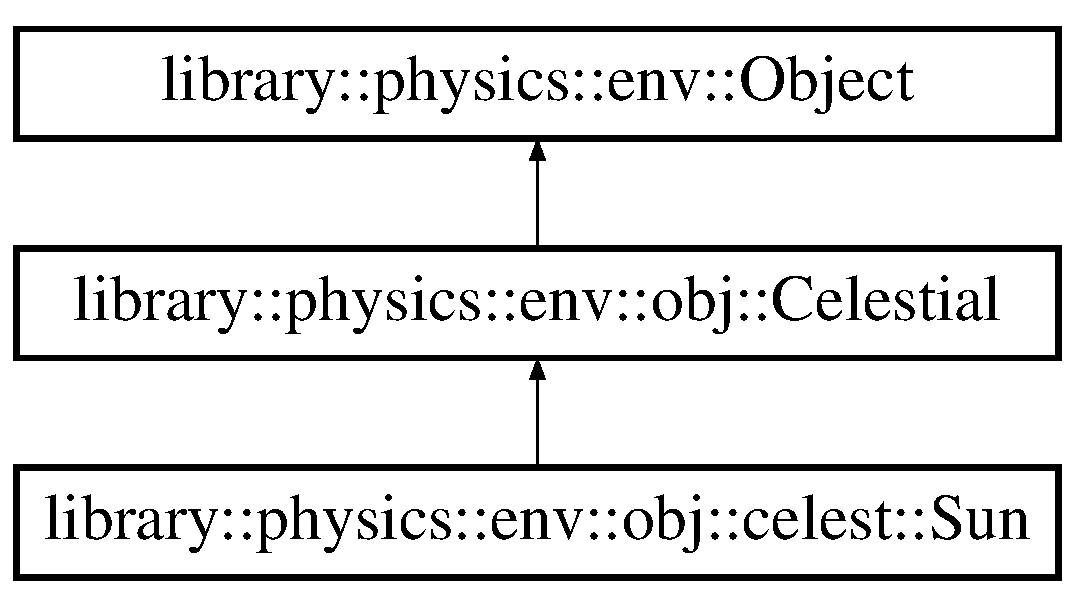
\includegraphics[height=3.000000cm]{classlibrary_1_1physics_1_1env_1_1obj_1_1celest_1_1_sun}
\end{center}
\end{figure}
\subsection*{Public Member Functions}
\begin{DoxyCompactItemize}
\item 
\hyperlink{classlibrary_1_1physics_1_1env_1_1obj_1_1celest_1_1_sun_ada5eefc36e00d3e68d60c94b85144388}{Sun} (const Shared$<$ \hyperlink{classlibrary_1_1physics_1_1env_1_1_ephemeris}{Ephemeris} $>$ \&an\+Ephemeris, const Shared$<$ \hyperlink{namespacelibrary_1_1physics_1_1env_1_1obj_1_1celest_ac63145c8cbe868bd79be8f6f423c8cf4}{Gravitational\+Model} $>$ \&a\+Gravitational\+Model, const \hyperlink{classlibrary_1_1physics_1_1time_1_1_instant}{Instant} \&an\+Instant)
\item 
virtual \hyperlink{classlibrary_1_1physics_1_1env_1_1obj_1_1celest_1_1_sun_a34a14e47bbbc26292809dba9c8d1ece8}{$\sim$\+Sun} () override
\item 
virtual \hyperlink{classlibrary_1_1physics_1_1env_1_1obj_1_1celest_1_1_sun}{Sun} $\ast$ \hyperlink{classlibrary_1_1physics_1_1env_1_1obj_1_1celest_1_1_sun_a79fa2d336dad399c3d933b0f5a2f9427}{clone} () const override
\end{DoxyCompactItemize}
\subsection*{Static Public Member Functions}
\begin{DoxyCompactItemize}
\item 
static \hyperlink{classlibrary_1_1physics_1_1env_1_1obj_1_1celest_1_1_sun}{Sun} \hyperlink{classlibrary_1_1physics_1_1env_1_1obj_1_1celest_1_1_sun_a4854f1ce74cbabb804d0084b71e76bcf}{Default} ()
\end{DoxyCompactItemize}
\subsection*{Static Public Attributes}
\begin{DoxyCompactItemize}
\item 
static \hyperlink{classlibrary_1_1physics_1_1units_1_1_derived}{Derived} \hyperlink{classlibrary_1_1physics_1_1env_1_1obj_1_1celest_1_1_sun_abdaf89ab0651e1cd00701de41f728427}{Gravitational\+Parameter} = \hyperlink{classlibrary_1_1physics_1_1units_1_1_derived}{Derived}(132712440018e9, \{ Length\+::\+Unit\+::\+Meter, Derived\+::\+Order(3), Mass\+::\+Unit\+::\+Undefined, Derived\+::\+Order\+::\+Zero(), Time\+::\+Unit\+::\+Second, Derived\+::\+Order(-\/2), Angle\+::\+Unit\+::\+Undefined, Derived\+::\+Order\+::\+Zero() \})
\item 
static \hyperlink{classlibrary_1_1physics_1_1units_1_1_length}{Length} \hyperlink{classlibrary_1_1physics_1_1env_1_1obj_1_1celest_1_1_sun_a48679ac65c067b77adf005ce9ca5cfca}{Equatorial\+Radius} = \hyperlink{classlibrary_1_1physics_1_1units_1_1_length_ad523a3737d5c3f23a64588eac83f2148}{Length\+::\+Meters}(6.\+955e8)
\item 
static Real \hyperlink{classlibrary_1_1physics_1_1env_1_1obj_1_1celest_1_1_sun_a48caf436831d176c692b6aa714b77676}{Flattening} = 0.\+0
\end{DoxyCompactItemize}
\subsection*{Additional Inherited Members}


\subsection{Constructor \& Destructor Documentation}
\mbox{\Hypertarget{classlibrary_1_1physics_1_1env_1_1obj_1_1celest_1_1_sun_ada5eefc36e00d3e68d60c94b85144388}\label{classlibrary_1_1physics_1_1env_1_1obj_1_1celest_1_1_sun_ada5eefc36e00d3e68d60c94b85144388}} 
\index{library\+::physics\+::env\+::obj\+::celest\+::\+Sun@{library\+::physics\+::env\+::obj\+::celest\+::\+Sun}!Sun@{Sun}}
\index{Sun@{Sun}!library\+::physics\+::env\+::obj\+::celest\+::\+Sun@{library\+::physics\+::env\+::obj\+::celest\+::\+Sun}}
\subsubsection{\texorpdfstring{Sun()}{Sun()}}
{\footnotesize\ttfamily library\+::physics\+::env\+::obj\+::celest\+::\+Sun\+::\+Sun (\begin{DoxyParamCaption}\item[{const Shared$<$ \hyperlink{classlibrary_1_1physics_1_1env_1_1_ephemeris}{Ephemeris} $>$ \&}]{an\+Ephemeris,  }\item[{const Shared$<$ \hyperlink{namespacelibrary_1_1physics_1_1env_1_1obj_1_1celest_ac63145c8cbe868bd79be8f6f423c8cf4}{Gravitational\+Model} $>$ \&}]{a\+Gravitational\+Model,  }\item[{const \hyperlink{classlibrary_1_1physics_1_1time_1_1_instant}{Instant} \&}]{an\+Instant }\end{DoxyParamCaption})}

\mbox{\Hypertarget{classlibrary_1_1physics_1_1env_1_1obj_1_1celest_1_1_sun_a34a14e47bbbc26292809dba9c8d1ece8}\label{classlibrary_1_1physics_1_1env_1_1obj_1_1celest_1_1_sun_a34a14e47bbbc26292809dba9c8d1ece8}} 
\index{library\+::physics\+::env\+::obj\+::celest\+::\+Sun@{library\+::physics\+::env\+::obj\+::celest\+::\+Sun}!````~Sun@{$\sim$\+Sun}}
\index{````~Sun@{$\sim$\+Sun}!library\+::physics\+::env\+::obj\+::celest\+::\+Sun@{library\+::physics\+::env\+::obj\+::celest\+::\+Sun}}
\subsubsection{\texorpdfstring{$\sim$\+Sun()}{~Sun()}}
{\footnotesize\ttfamily library\+::physics\+::env\+::obj\+::celest\+::\+Sun\+::$\sim$\+Sun (\begin{DoxyParamCaption}{ }\end{DoxyParamCaption})\hspace{0.3cm}{\ttfamily [override]}, {\ttfamily [virtual]}}



\subsection{Member Function Documentation}
\mbox{\Hypertarget{classlibrary_1_1physics_1_1env_1_1obj_1_1celest_1_1_sun_a79fa2d336dad399c3d933b0f5a2f9427}\label{classlibrary_1_1physics_1_1env_1_1obj_1_1celest_1_1_sun_a79fa2d336dad399c3d933b0f5a2f9427}} 
\index{library\+::physics\+::env\+::obj\+::celest\+::\+Sun@{library\+::physics\+::env\+::obj\+::celest\+::\+Sun}!clone@{clone}}
\index{clone@{clone}!library\+::physics\+::env\+::obj\+::celest\+::\+Sun@{library\+::physics\+::env\+::obj\+::celest\+::\+Sun}}
\subsubsection{\texorpdfstring{clone()}{clone()}}
{\footnotesize\ttfamily \hyperlink{classlibrary_1_1physics_1_1env_1_1obj_1_1celest_1_1_sun}{Sun} $\ast$ library\+::physics\+::env\+::obj\+::celest\+::\+Sun\+::clone (\begin{DoxyParamCaption}{ }\end{DoxyParamCaption}) const\hspace{0.3cm}{\ttfamily [override]}, {\ttfamily [virtual]}}



Reimplemented from \hyperlink{classlibrary_1_1physics_1_1env_1_1obj_1_1_celestial_aaf8aa41a0ff9336eba62c07e3c27f82d}{library\+::physics\+::env\+::obj\+::\+Celestial}.

\mbox{\Hypertarget{classlibrary_1_1physics_1_1env_1_1obj_1_1celest_1_1_sun_a4854f1ce74cbabb804d0084b71e76bcf}\label{classlibrary_1_1physics_1_1env_1_1obj_1_1celest_1_1_sun_a4854f1ce74cbabb804d0084b71e76bcf}} 
\index{library\+::physics\+::env\+::obj\+::celest\+::\+Sun@{library\+::physics\+::env\+::obj\+::celest\+::\+Sun}!Default@{Default}}
\index{Default@{Default}!library\+::physics\+::env\+::obj\+::celest\+::\+Sun@{library\+::physics\+::env\+::obj\+::celest\+::\+Sun}}
\subsubsection{\texorpdfstring{Default()}{Default()}}
{\footnotesize\ttfamily \hyperlink{classlibrary_1_1physics_1_1env_1_1obj_1_1celest_1_1_sun}{Sun} library\+::physics\+::env\+::obj\+::celest\+::\+Sun\+::\+Default (\begin{DoxyParamCaption}{ }\end{DoxyParamCaption})\hspace{0.3cm}{\ttfamily [static]}}



\subsection{Member Data Documentation}
\mbox{\Hypertarget{classlibrary_1_1physics_1_1env_1_1obj_1_1celest_1_1_sun_a48679ac65c067b77adf005ce9ca5cfca}\label{classlibrary_1_1physics_1_1env_1_1obj_1_1celest_1_1_sun_a48679ac65c067b77adf005ce9ca5cfca}} 
\index{library\+::physics\+::env\+::obj\+::celest\+::\+Sun@{library\+::physics\+::env\+::obj\+::celest\+::\+Sun}!Equatorial\+Radius@{Equatorial\+Radius}}
\index{Equatorial\+Radius@{Equatorial\+Radius}!library\+::physics\+::env\+::obj\+::celest\+::\+Sun@{library\+::physics\+::env\+::obj\+::celest\+::\+Sun}}
\subsubsection{\texorpdfstring{Equatorial\+Radius}{EquatorialRadius}}
{\footnotesize\ttfamily \hyperlink{classlibrary_1_1physics_1_1units_1_1_length}{Length} library\+::physics\+::env\+::obj\+::celest\+::\+Sun\+::\+Equatorial\+Radius = \hyperlink{classlibrary_1_1physics_1_1units_1_1_length_ad523a3737d5c3f23a64588eac83f2148}{Length\+::\+Meters}(6.\+955e8)\hspace{0.3cm}{\ttfamily [static]}}

\mbox{\Hypertarget{classlibrary_1_1physics_1_1env_1_1obj_1_1celest_1_1_sun_a48caf436831d176c692b6aa714b77676}\label{classlibrary_1_1physics_1_1env_1_1obj_1_1celest_1_1_sun_a48caf436831d176c692b6aa714b77676}} 
\index{library\+::physics\+::env\+::obj\+::celest\+::\+Sun@{library\+::physics\+::env\+::obj\+::celest\+::\+Sun}!Flattening@{Flattening}}
\index{Flattening@{Flattening}!library\+::physics\+::env\+::obj\+::celest\+::\+Sun@{library\+::physics\+::env\+::obj\+::celest\+::\+Sun}}
\subsubsection{\texorpdfstring{Flattening}{Flattening}}
{\footnotesize\ttfamily Real library\+::physics\+::env\+::obj\+::celest\+::\+Sun\+::\+Flattening = 0.\+0\hspace{0.3cm}{\ttfamily [static]}}

\mbox{\Hypertarget{classlibrary_1_1physics_1_1env_1_1obj_1_1celest_1_1_sun_abdaf89ab0651e1cd00701de41f728427}\label{classlibrary_1_1physics_1_1env_1_1obj_1_1celest_1_1_sun_abdaf89ab0651e1cd00701de41f728427}} 
\index{library\+::physics\+::env\+::obj\+::celest\+::\+Sun@{library\+::physics\+::env\+::obj\+::celest\+::\+Sun}!Gravitational\+Parameter@{Gravitational\+Parameter}}
\index{Gravitational\+Parameter@{Gravitational\+Parameter}!library\+::physics\+::env\+::obj\+::celest\+::\+Sun@{library\+::physics\+::env\+::obj\+::celest\+::\+Sun}}
\subsubsection{\texorpdfstring{Gravitational\+Parameter}{GravitationalParameter}}
{\footnotesize\ttfamily \hyperlink{classlibrary_1_1physics_1_1units_1_1_derived}{Derived} library\+::physics\+::env\+::obj\+::celest\+::\+Sun\+::\+Gravitational\+Parameter = \hyperlink{classlibrary_1_1physics_1_1units_1_1_derived}{Derived}(132712440018e9, \{ Length\+::\+Unit\+::\+Meter, Derived\+::\+Order(3), Mass\+::\+Unit\+::\+Undefined, Derived\+::\+Order\+::\+Zero(), Time\+::\+Unit\+::\+Second, Derived\+::\+Order(-\/2), Angle\+::\+Unit\+::\+Undefined, Derived\+::\+Order\+::\+Zero() \})\hspace{0.3cm}{\ttfamily [static]}}



The documentation for this class was generated from the following files\+:\begin{DoxyCompactItemize}
\item 
include/\+Library/\+Physics/\+Environment/\+Objects/\+Celestial\+Bodies/\hyperlink{_sun_8hpp}{Sun.\+hpp}\item 
src/\+Library/\+Physics/\+Environment/\+Objects/\+Celestial\+Bodies/\hyperlink{_sun_8cpp}{Sun.\+cpp}\end{DoxyCompactItemize}

\hypertarget{classlibrary_1_1physics_1_1coord_1_1frame_1_1provider_1_1_t_e_m_e}{}\section{library\+:\+:physics\+:\+:coord\+:\+:frame\+:\+:provider\+:\+:T\+E\+ME Class Reference}
\label{classlibrary_1_1physics_1_1coord_1_1frame_1_1provider_1_1_t_e_m_e}\index{library\+::physics\+::coord\+::frame\+::provider\+::\+T\+E\+ME@{library\+::physics\+::coord\+::frame\+::provider\+::\+T\+E\+ME}}


True Equator Mean Equinox (\hyperlink{classlibrary_1_1physics_1_1coord_1_1frame_1_1provider_1_1_t_e_m_e}{T\+E\+ME}) frame provider.  




{\ttfamily \#include $<$T\+E\+M\+E.\+hpp$>$}

Inheritance diagram for library\+:\+:physics\+:\+:coord\+:\+:frame\+:\+:provider\+:\+:T\+E\+ME\+:\begin{figure}[H]
\begin{center}
\leavevmode
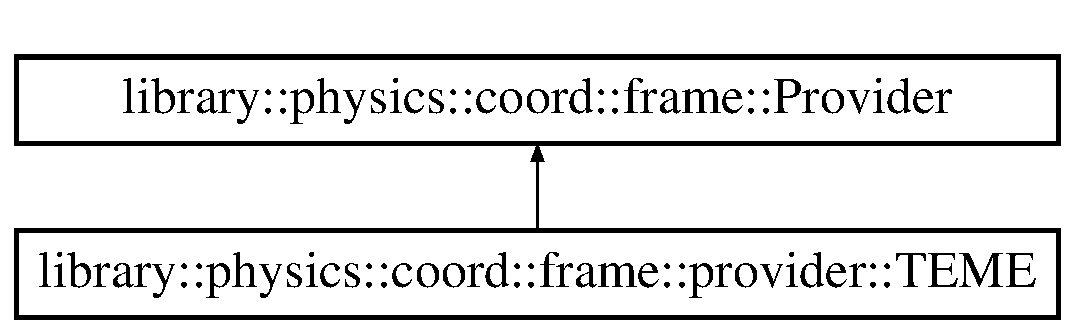
\includegraphics[height=2.000000cm]{classlibrary_1_1physics_1_1coord_1_1frame_1_1provider_1_1_t_e_m_e}
\end{center}
\end{figure}
\subsection*{Public Member Functions}
\begin{DoxyCompactItemize}
\item 
\hyperlink{classlibrary_1_1physics_1_1coord_1_1frame_1_1provider_1_1_t_e_m_e_a2b7c35dac37e2c95c280762b3c4d5f1a}{T\+E\+ME} ()
\item 
virtual \hyperlink{classlibrary_1_1physics_1_1coord_1_1frame_1_1provider_1_1_t_e_m_e_a945c6d66994dad1572e0895111fcfaba}{$\sim$\+T\+E\+ME} () override
\item 
virtual \hyperlink{classlibrary_1_1physics_1_1coord_1_1frame_1_1provider_1_1_t_e_m_e}{T\+E\+ME} $\ast$ \hyperlink{classlibrary_1_1physics_1_1coord_1_1frame_1_1provider_1_1_t_e_m_e_a606d0c4cad7df776e848fd3670e5cc7f}{clone} () const override
\item 
virtual bool \hyperlink{classlibrary_1_1physics_1_1coord_1_1frame_1_1provider_1_1_t_e_m_e_a8c52ea8c59a669197234383e4bfa54b6}{is\+Defined} () const override
\item 
virtual \hyperlink{classlibrary_1_1physics_1_1coord_1_1_transform}{Transform} \hyperlink{classlibrary_1_1physics_1_1coord_1_1frame_1_1provider_1_1_t_e_m_e_a78bd46fa8118d7220ab16a4ca2195299}{get\+Transform\+At} (const \hyperlink{classlibrary_1_1physics_1_1time_1_1_instant}{Instant} \&an\+Instant) const override
\end{DoxyCompactItemize}


\subsection{Detailed Description}
True Equator Mean Equinox (\hyperlink{classlibrary_1_1physics_1_1coord_1_1frame_1_1provider_1_1_t_e_m_e}{T\+E\+ME}) frame provider. 

\begin{DoxyNote}{Note}
This frame should only be used with Two-\/\+Line Elements (T\+LE).
\end{DoxyNote}
https\+://en.wikipedia.\+org/wiki/\+Earth-\/centered\+\_\+inertial 

\subsection{Constructor \& Destructor Documentation}
\mbox{\Hypertarget{classlibrary_1_1physics_1_1coord_1_1frame_1_1provider_1_1_t_e_m_e_a2b7c35dac37e2c95c280762b3c4d5f1a}\label{classlibrary_1_1physics_1_1coord_1_1frame_1_1provider_1_1_t_e_m_e_a2b7c35dac37e2c95c280762b3c4d5f1a}} 
\index{library\+::physics\+::coord\+::frame\+::provider\+::\+T\+E\+ME@{library\+::physics\+::coord\+::frame\+::provider\+::\+T\+E\+ME}!T\+E\+ME@{T\+E\+ME}}
\index{T\+E\+ME@{T\+E\+ME}!library\+::physics\+::coord\+::frame\+::provider\+::\+T\+E\+ME@{library\+::physics\+::coord\+::frame\+::provider\+::\+T\+E\+ME}}
\subsubsection{\texorpdfstring{T\+E\+M\+E()}{TEME()}}
{\footnotesize\ttfamily library\+::physics\+::coord\+::frame\+::provider\+::\+T\+E\+M\+E\+::\+T\+E\+ME (\begin{DoxyParamCaption}{ }\end{DoxyParamCaption})}

\mbox{\Hypertarget{classlibrary_1_1physics_1_1coord_1_1frame_1_1provider_1_1_t_e_m_e_a945c6d66994dad1572e0895111fcfaba}\label{classlibrary_1_1physics_1_1coord_1_1frame_1_1provider_1_1_t_e_m_e_a945c6d66994dad1572e0895111fcfaba}} 
\index{library\+::physics\+::coord\+::frame\+::provider\+::\+T\+E\+ME@{library\+::physics\+::coord\+::frame\+::provider\+::\+T\+E\+ME}!````~T\+E\+ME@{$\sim$\+T\+E\+ME}}
\index{````~T\+E\+ME@{$\sim$\+T\+E\+ME}!library\+::physics\+::coord\+::frame\+::provider\+::\+T\+E\+ME@{library\+::physics\+::coord\+::frame\+::provider\+::\+T\+E\+ME}}
\subsubsection{\texorpdfstring{$\sim$\+T\+E\+M\+E()}{~TEME()}}
{\footnotesize\ttfamily library\+::physics\+::coord\+::frame\+::provider\+::\+T\+E\+M\+E\+::$\sim$\+T\+E\+ME (\begin{DoxyParamCaption}{ }\end{DoxyParamCaption})\hspace{0.3cm}{\ttfamily [override]}, {\ttfamily [virtual]}}



\subsection{Member Function Documentation}
\mbox{\Hypertarget{classlibrary_1_1physics_1_1coord_1_1frame_1_1provider_1_1_t_e_m_e_a606d0c4cad7df776e848fd3670e5cc7f}\label{classlibrary_1_1physics_1_1coord_1_1frame_1_1provider_1_1_t_e_m_e_a606d0c4cad7df776e848fd3670e5cc7f}} 
\index{library\+::physics\+::coord\+::frame\+::provider\+::\+T\+E\+ME@{library\+::physics\+::coord\+::frame\+::provider\+::\+T\+E\+ME}!clone@{clone}}
\index{clone@{clone}!library\+::physics\+::coord\+::frame\+::provider\+::\+T\+E\+ME@{library\+::physics\+::coord\+::frame\+::provider\+::\+T\+E\+ME}}
\subsubsection{\texorpdfstring{clone()}{clone()}}
{\footnotesize\ttfamily \hyperlink{classlibrary_1_1physics_1_1coord_1_1frame_1_1provider_1_1_t_e_m_e}{T\+E\+ME} $\ast$ library\+::physics\+::coord\+::frame\+::provider\+::\+T\+E\+M\+E\+::clone (\begin{DoxyParamCaption}{ }\end{DoxyParamCaption}) const\hspace{0.3cm}{\ttfamily [override]}, {\ttfamily [virtual]}}



Implements \hyperlink{classlibrary_1_1physics_1_1coord_1_1frame_1_1_provider_ab8eee40c8ef4aee0b57bedf458f4934e}{library\+::physics\+::coord\+::frame\+::\+Provider}.

\mbox{\Hypertarget{classlibrary_1_1physics_1_1coord_1_1frame_1_1provider_1_1_t_e_m_e_a78bd46fa8118d7220ab16a4ca2195299}\label{classlibrary_1_1physics_1_1coord_1_1frame_1_1provider_1_1_t_e_m_e_a78bd46fa8118d7220ab16a4ca2195299}} 
\index{library\+::physics\+::coord\+::frame\+::provider\+::\+T\+E\+ME@{library\+::physics\+::coord\+::frame\+::provider\+::\+T\+E\+ME}!get\+Transform\+At@{get\+Transform\+At}}
\index{get\+Transform\+At@{get\+Transform\+At}!library\+::physics\+::coord\+::frame\+::provider\+::\+T\+E\+ME@{library\+::physics\+::coord\+::frame\+::provider\+::\+T\+E\+ME}}
\subsubsection{\texorpdfstring{get\+Transform\+At()}{getTransformAt()}}
{\footnotesize\ttfamily \hyperlink{classlibrary_1_1physics_1_1coord_1_1_transform}{Transform} library\+::physics\+::coord\+::frame\+::provider\+::\+T\+E\+M\+E\+::get\+Transform\+At (\begin{DoxyParamCaption}\item[{const \hyperlink{classlibrary_1_1physics_1_1time_1_1_instant}{Instant} \&}]{an\+Instant }\end{DoxyParamCaption}) const\hspace{0.3cm}{\ttfamily [override]}, {\ttfamily [virtual]}}



Implements \hyperlink{classlibrary_1_1physics_1_1coord_1_1frame_1_1_provider_a796fd2dd337f1304a0e9acf573ce2550}{library\+::physics\+::coord\+::frame\+::\+Provider}.

\mbox{\Hypertarget{classlibrary_1_1physics_1_1coord_1_1frame_1_1provider_1_1_t_e_m_e_a8c52ea8c59a669197234383e4bfa54b6}\label{classlibrary_1_1physics_1_1coord_1_1frame_1_1provider_1_1_t_e_m_e_a8c52ea8c59a669197234383e4bfa54b6}} 
\index{library\+::physics\+::coord\+::frame\+::provider\+::\+T\+E\+ME@{library\+::physics\+::coord\+::frame\+::provider\+::\+T\+E\+ME}!is\+Defined@{is\+Defined}}
\index{is\+Defined@{is\+Defined}!library\+::physics\+::coord\+::frame\+::provider\+::\+T\+E\+ME@{library\+::physics\+::coord\+::frame\+::provider\+::\+T\+E\+ME}}
\subsubsection{\texorpdfstring{is\+Defined()}{isDefined()}}
{\footnotesize\ttfamily bool library\+::physics\+::coord\+::frame\+::provider\+::\+T\+E\+M\+E\+::is\+Defined (\begin{DoxyParamCaption}{ }\end{DoxyParamCaption}) const\hspace{0.3cm}{\ttfamily [override]}, {\ttfamily [virtual]}}



Implements \hyperlink{classlibrary_1_1physics_1_1coord_1_1frame_1_1_provider_ae7cd093febf2b20f71400f9f79442774}{library\+::physics\+::coord\+::frame\+::\+Provider}.



The documentation for this class was generated from the following files\+:\begin{DoxyCompactItemize}
\item 
include/\+Library/\+Physics/\+Coordinate/\+Frame/\+Providers/\hyperlink{_t_e_m_e_8hpp}{T\+E\+M\+E.\+hpp}\item 
src/\+Library/\+Physics/\+Coordinate/\+Frame/\+Providers/\hyperlink{_t_e_m_e_8cpp}{T\+E\+M\+E.\+cpp}\end{DoxyCompactItemize}

\hypertarget{classlibrary_1_1physics_1_1time_1_1_time}{}\section{library\+:\+:physics\+:\+:time\+:\+:Time Class Reference}
\label{classlibrary_1_1physics_1_1time_1_1_time}\index{library\+::physics\+::time\+::\+Time@{library\+::physics\+::time\+::\+Time}}


\hyperlink{classlibrary_1_1physics_1_1time_1_1_time}{Time} as hour, minute, second, millisecond, microsecond and nanosecond.  




{\ttfamily \#include $<$Time.\+hpp$>$}

\subsection*{Public Types}
\begin{DoxyCompactItemize}
\item 
enum \hyperlink{classlibrary_1_1physics_1_1time_1_1_time_a7cfbcbb1d5d0c536e28e61f1e7cbf1c8}{Format} \{ \hyperlink{classlibrary_1_1physics_1_1time_1_1_time_a7cfbcbb1d5d0c536e28e61f1e7cbf1c8aec0fc0100c4fc1ce4eea230c3dc10360}{Format\+::\+Undefined}, 
\hyperlink{classlibrary_1_1physics_1_1time_1_1_time_a7cfbcbb1d5d0c536e28e61f1e7cbf1c8aeb6d8ae6f20283755b339c0dc273988b}{Format\+::\+Standard}, 
\hyperlink{classlibrary_1_1physics_1_1time_1_1_time_a7cfbcbb1d5d0c536e28e61f1e7cbf1c8a35b6786739efcdc5a74ab1dca29d3b6b}{Format\+::\+I\+S\+O8601}
 \}\begin{DoxyCompactList}\small\item\em \hyperlink{classlibrary_1_1physics_1_1time_1_1_time}{Time} format. \end{DoxyCompactList}
\end{DoxyCompactItemize}
\subsection*{Public Member Functions}
\begin{DoxyCompactItemize}
\item 
\hyperlink{classlibrary_1_1physics_1_1time_1_1_time_a46a4b9be1451041ae65332f04db21c4b}{Time} (Uint8 an\+Hour, Uint8 a\+Minute, Uint8 a\+Second, Uint16 a\+Millisecond=0, Uint16 a\+Microsecond=0, Uint16 a\+Nanosecond=0)
\begin{DoxyCompactList}\small\item\em Constructor. \end{DoxyCompactList}\item 
bool \hyperlink{classlibrary_1_1physics_1_1time_1_1_time_ac566f208b63b58b5dae1328b4c24fbe6}{operator==} (const \hyperlink{classlibrary_1_1physics_1_1time_1_1_time}{Time} \&a\+Time) const
\begin{DoxyCompactList}\small\item\em Equal to operator. \end{DoxyCompactList}\item 
bool \hyperlink{classlibrary_1_1physics_1_1time_1_1_time_af2caee50ce2d4abd157645052a090db1}{operator!=} (const \hyperlink{classlibrary_1_1physics_1_1time_1_1_time}{Time} \&a\+Time) const
\begin{DoxyCompactList}\small\item\em Not equal to operator. \end{DoxyCompactList}\item 
bool \hyperlink{classlibrary_1_1physics_1_1time_1_1_time_a45736fe7072e922a9d9c3829c7517b88}{is\+Defined} () const
\begin{DoxyCompactList}\small\item\em Check if time is defined. \end{DoxyCompactList}\item 
Uint8 \hyperlink{classlibrary_1_1physics_1_1time_1_1_time_a3744d684384aabf0122dcac098e480fa}{get\+Hour} () const
\begin{DoxyCompactList}\small\item\em Get hour (0 -\/ 23) \end{DoxyCompactList}\item 
Uint8 \hyperlink{classlibrary_1_1physics_1_1time_1_1_time_a322ff06ee6674a14331848b9960dfaff}{get\+Minute} () const
\begin{DoxyCompactList}\small\item\em Get minute (0 -\/ 59) \end{DoxyCompactList}\item 
Uint8 \hyperlink{classlibrary_1_1physics_1_1time_1_1_time_aca543eadd3112d54a0d014512f99e90a}{get\+Second} () const
\begin{DoxyCompactList}\small\item\em Get second (0 -\/ 60) \end{DoxyCompactList}\item 
Uint16 \hyperlink{classlibrary_1_1physics_1_1time_1_1_time_aba745cf1f96b5826e50f8a074af13369}{get\+Millisecond} () const
\begin{DoxyCompactList}\small\item\em Get millisecond (0 -\/ 999) \end{DoxyCompactList}\item 
Uint16 \hyperlink{classlibrary_1_1physics_1_1time_1_1_time_a10bc719a72442215d0f073afadc7b542}{get\+Microsecond} () const
\begin{DoxyCompactList}\small\item\em Get microsecond (0 -\/ 999) \end{DoxyCompactList}\item 
Uint16 \hyperlink{classlibrary_1_1physics_1_1time_1_1_time_a13de54324ffddc6f73e6e4ccc9149068}{get\+Nanosecond} () const
\begin{DoxyCompactList}\small\item\em Get nanosecond (0 -\/ 999) \end{DoxyCompactList}\item 
Real \hyperlink{classlibrary_1_1physics_1_1time_1_1_time_adfbd0fd8b766f43a6f3a8bdccd8852fb}{get\+Floating\+Seconds} () const
\begin{DoxyCompactList}\small\item\em Get floating seconds (0.\+0 -\/ 59.\+999999999) \end{DoxyCompactList}\item 
String \hyperlink{classlibrary_1_1physics_1_1time_1_1_time_a9cd369886bade37d48146afc0d7a2271}{to\+String} (const \hyperlink{classlibrary_1_1physics_1_1time_1_1_time_a7cfbcbb1d5d0c536e28e61f1e7cbf1c8}{Time\+::\+Format} \&a\+Format=\hyperlink{classlibrary_1_1physics_1_1time_1_1_time_a7cfbcbb1d5d0c536e28e61f1e7cbf1c8aeb6d8ae6f20283755b339c0dc273988b}{Time\+::\+Format\+::\+Standard}) const
\begin{DoxyCompactList}\small\item\em Get string representation of time. \end{DoxyCompactList}\item 
void \hyperlink{classlibrary_1_1physics_1_1time_1_1_time_a7e1d98631f94f394e0360921d52b0c87}{set\+Hour} (Uint8 an\+Hour)
\begin{DoxyCompactList}\small\item\em Set hour. \end{DoxyCompactList}\item 
void \hyperlink{classlibrary_1_1physics_1_1time_1_1_time_a62140a0b62a0d6264b4b1f65106e6d21}{set\+Minute} (Uint8 a\+Minute)
\begin{DoxyCompactList}\small\item\em Set minute. \end{DoxyCompactList}\item 
void \hyperlink{classlibrary_1_1physics_1_1time_1_1_time_add6193c6d0e3f4c0d9bdb78c1020fea2}{set\+Second} (Uint8 a\+Second)
\begin{DoxyCompactList}\small\item\em Set second. \end{DoxyCompactList}\item 
void \hyperlink{classlibrary_1_1physics_1_1time_1_1_time_a1813a36c2f988b97db039843201abc68}{set\+Millisecond} (Uint16 a\+Millisecond)
\begin{DoxyCompactList}\small\item\em Set millisecond. \end{DoxyCompactList}\item 
void \hyperlink{classlibrary_1_1physics_1_1time_1_1_time_a1cc4c14fc9e88909bca57724da4f5c46}{set\+Microsecond} (Uint16 a\+Microsecond)
\begin{DoxyCompactList}\small\item\em Set microsecond. \end{DoxyCompactList}\item 
void \hyperlink{classlibrary_1_1physics_1_1time_1_1_time_a2d941601ab94abc646d085e7958d1739}{set\+Nanosecond} (Uint16 a\+Nanosecond)
\begin{DoxyCompactList}\small\item\em Set nanosecond. \end{DoxyCompactList}\end{DoxyCompactItemize}
\subsection*{Static Public Member Functions}
\begin{DoxyCompactItemize}
\item 
static \hyperlink{classlibrary_1_1physics_1_1time_1_1_time}{Time} \hyperlink{classlibrary_1_1physics_1_1time_1_1_time_a6e8c7e4ea2d05a7c0a9e5e045ef45520}{Undefined} ()
\begin{DoxyCompactList}\small\item\em Constructs an undefined time. \end{DoxyCompactList}\item 
static \hyperlink{classlibrary_1_1physics_1_1time_1_1_time}{Time} \hyperlink{classlibrary_1_1physics_1_1time_1_1_time_a03dac8a95c9e8f64ef98c5370112b3b8}{Midnight} ()
\begin{DoxyCompactList}\small\item\em Constructs a time at midnight. \end{DoxyCompactList}\item 
static \hyperlink{classlibrary_1_1physics_1_1time_1_1_time}{Time} \hyperlink{classlibrary_1_1physics_1_1time_1_1_time_a3d67891fe71e3b5ba62c6517477e7698}{Noon} ()
\begin{DoxyCompactList}\small\item\em Constructs a time at noon. \end{DoxyCompactList}\item 
static \hyperlink{classlibrary_1_1physics_1_1time_1_1_time}{Time} \hyperlink{classlibrary_1_1physics_1_1time_1_1_time_a0756ad7ca377adc810b7515411657e3b}{Parse} (const String \&a\+String, const \hyperlink{classlibrary_1_1physics_1_1time_1_1_time_a7cfbcbb1d5d0c536e28e61f1e7cbf1c8}{Time\+::\+Format} \&a\+Format=\hyperlink{classlibrary_1_1physics_1_1time_1_1_time_a7cfbcbb1d5d0c536e28e61f1e7cbf1c8aec0fc0100c4fc1ce4eea230c3dc10360}{Time\+::\+Format\+::\+Undefined})
\begin{DoxyCompactList}\small\item\em Constructs a time from a string representation. \end{DoxyCompactList}\end{DoxyCompactItemize}
\subsection*{Friends}
\begin{DoxyCompactItemize}
\item 
std\+::ostream \& \hyperlink{classlibrary_1_1physics_1_1time_1_1_time_a181948621d8fe0d85bdfc97af30b62fb}{operator$<$$<$} (std\+::ostream \&an\+Output\+Stream, const \hyperlink{classlibrary_1_1physics_1_1time_1_1_time}{Time} \&a\+Time)
\begin{DoxyCompactList}\small\item\em Output stream operator. \end{DoxyCompactList}\end{DoxyCompactItemize}


\subsection{Detailed Description}
\hyperlink{classlibrary_1_1physics_1_1time_1_1_time}{Time} as hour, minute, second, millisecond, microsecond and nanosecond. 

\subsection{Member Enumeration Documentation}
\mbox{\Hypertarget{classlibrary_1_1physics_1_1time_1_1_time_a7cfbcbb1d5d0c536e28e61f1e7cbf1c8}\label{classlibrary_1_1physics_1_1time_1_1_time_a7cfbcbb1d5d0c536e28e61f1e7cbf1c8}} 
\index{library\+::physics\+::time\+::\+Time@{library\+::physics\+::time\+::\+Time}!Format@{Format}}
\index{Format@{Format}!library\+::physics\+::time\+::\+Time@{library\+::physics\+::time\+::\+Time}}
\subsubsection{\texorpdfstring{Format}{Format}}
{\footnotesize\ttfamily enum \hyperlink{classlibrary_1_1physics_1_1time_1_1_time_a7cfbcbb1d5d0c536e28e61f1e7cbf1c8}{library\+::physics\+::time\+::\+Time\+::\+Format}\hspace{0.3cm}{\ttfamily [strong]}}



\hyperlink{classlibrary_1_1physics_1_1time_1_1_time}{Time} format. 

\begin{DoxyEnumFields}{Enumerator}
\raisebox{\heightof{T}}[0pt][0pt]{\index{Undefined@{Undefined}!library\+::physics\+::time\+::\+Time@{library\+::physics\+::time\+::\+Time}}\index{library\+::physics\+::time\+::\+Time@{library\+::physics\+::time\+::\+Time}!Undefined@{Undefined}}}\mbox{\Hypertarget{classlibrary_1_1physics_1_1time_1_1_time_a7cfbcbb1d5d0c536e28e61f1e7cbf1c8aec0fc0100c4fc1ce4eea230c3dc10360}\label{classlibrary_1_1physics_1_1time_1_1_time_a7cfbcbb1d5d0c536e28e61f1e7cbf1c8aec0fc0100c4fc1ce4eea230c3dc10360}} 
Undefined&Undefined format. \\
\hline

\raisebox{\heightof{T}}[0pt][0pt]{\index{Standard@{Standard}!library\+::physics\+::time\+::\+Time@{library\+::physics\+::time\+::\+Time}}\index{library\+::physics\+::time\+::\+Time@{library\+::physics\+::time\+::\+Time}!Standard@{Standard}}}\mbox{\Hypertarget{classlibrary_1_1physics_1_1time_1_1_time_a7cfbcbb1d5d0c536e28e61f1e7cbf1c8aeb6d8ae6f20283755b339c0dc273988b}\label{classlibrary_1_1physics_1_1time_1_1_time_a7cfbcbb1d5d0c536e28e61f1e7cbf1c8aeb6d8ae6f20283755b339c0dc273988b}} 
Standard&Standard format (hh\+:mm\+:ss.\+sss.\+sss.\+sss) \\
\hline

\raisebox{\heightof{T}}[0pt][0pt]{\index{I\+S\+O8601@{I\+S\+O8601}!library\+::physics\+::time\+::\+Time@{library\+::physics\+::time\+::\+Time}}\index{library\+::physics\+::time\+::\+Time@{library\+::physics\+::time\+::\+Time}!I\+S\+O8601@{I\+S\+O8601}}}\mbox{\Hypertarget{classlibrary_1_1physics_1_1time_1_1_time_a7cfbcbb1d5d0c536e28e61f1e7cbf1c8a35b6786739efcdc5a74ab1dca29d3b6b}\label{classlibrary_1_1physics_1_1time_1_1_time_a7cfbcbb1d5d0c536e28e61f1e7cbf1c8a35b6786739efcdc5a74ab1dca29d3b6b}} 
I\+S\+O8601&I\+SO 8601 format (hh\+:mm\+:ss.\+sssssssss) \\
\hline

\end{DoxyEnumFields}


\subsection{Constructor \& Destructor Documentation}
\mbox{\Hypertarget{classlibrary_1_1physics_1_1time_1_1_time_a46a4b9be1451041ae65332f04db21c4b}\label{classlibrary_1_1physics_1_1time_1_1_time_a46a4b9be1451041ae65332f04db21c4b}} 
\index{library\+::physics\+::time\+::\+Time@{library\+::physics\+::time\+::\+Time}!Time@{Time}}
\index{Time@{Time}!library\+::physics\+::time\+::\+Time@{library\+::physics\+::time\+::\+Time}}
\subsubsection{\texorpdfstring{Time()}{Time()}}
{\footnotesize\ttfamily library\+::physics\+::time\+::\+Time\+::\+Time (\begin{DoxyParamCaption}\item[{Uint8}]{an\+Hour,  }\item[{Uint8}]{a\+Minute,  }\item[{Uint8}]{a\+Second,  }\item[{Uint16}]{a\+Millisecond = {\ttfamily 0},  }\item[{Uint16}]{a\+Microsecond = {\ttfamily 0},  }\item[{Uint16}]{a\+Nanosecond = {\ttfamily 0} }\end{DoxyParamCaption})}



Constructor. 


\begin{DoxyCode}
\hyperlink{classlibrary_1_1physics_1_1time_1_1_time_a46a4b9be1451041ae65332f04db21c4b}{Time} time \{ 12, 34, 56 \} ; \textcolor{comment}{// 12:34:56.000.000.000}
\hyperlink{classlibrary_1_1physics_1_1time_1_1_time_a46a4b9be1451041ae65332f04db21c4b}{Time} time \{ 12, 34, 56, 123, 456, 789 \} ; \textcolor{comment}{// 12:34:56.123.456.789}
\end{DoxyCode}



\begin{DoxyParams}[1]{Parameters}
\mbox{\tt in}  & {\em an\+Hour} & An hour count (0 -\/ 23) \\
\hline
\mbox{\tt in}  & {\em a\+Minute} & A minute count (0 -\/ 59) \\
\hline
\mbox{\tt in}  & {\em a\+Second} & A second count (0 -\/ 60) \\
\hline
\mbox{\tt in}  & {\em (optional)} & a\+Millisecond A millisecond count (0 -\/ 999) \\
\hline
\mbox{\tt in}  & {\em (optional)} & a\+Microsecond A microsecond count (0 -\/ 999) \\
\hline
\mbox{\tt in}  & {\em (optional)} & a\+Nanosecond A nanosecond count (0 -\/ 999) \\
\hline
\end{DoxyParams}


\subsection{Member Function Documentation}
\mbox{\Hypertarget{classlibrary_1_1physics_1_1time_1_1_time_adfbd0fd8b766f43a6f3a8bdccd8852fb}\label{classlibrary_1_1physics_1_1time_1_1_time_adfbd0fd8b766f43a6f3a8bdccd8852fb}} 
\index{library\+::physics\+::time\+::\+Time@{library\+::physics\+::time\+::\+Time}!get\+Floating\+Seconds@{get\+Floating\+Seconds}}
\index{get\+Floating\+Seconds@{get\+Floating\+Seconds}!library\+::physics\+::time\+::\+Time@{library\+::physics\+::time\+::\+Time}}
\subsubsection{\texorpdfstring{get\+Floating\+Seconds()}{getFloatingSeconds()}}
{\footnotesize\ttfamily Real library\+::physics\+::time\+::\+Time\+::get\+Floating\+Seconds (\begin{DoxyParamCaption}{ }\end{DoxyParamCaption}) const}



Get floating seconds (0.\+0 -\/ 59.\+999999999) 

\begin{DoxyReturn}{Returns}
Floating second 
\end{DoxyReturn}
\mbox{\Hypertarget{classlibrary_1_1physics_1_1time_1_1_time_a3744d684384aabf0122dcac098e480fa}\label{classlibrary_1_1physics_1_1time_1_1_time_a3744d684384aabf0122dcac098e480fa}} 
\index{library\+::physics\+::time\+::\+Time@{library\+::physics\+::time\+::\+Time}!get\+Hour@{get\+Hour}}
\index{get\+Hour@{get\+Hour}!library\+::physics\+::time\+::\+Time@{library\+::physics\+::time\+::\+Time}}
\subsubsection{\texorpdfstring{get\+Hour()}{getHour()}}
{\footnotesize\ttfamily Uint8 library\+::physics\+::time\+::\+Time\+::get\+Hour (\begin{DoxyParamCaption}{ }\end{DoxyParamCaption}) const}



Get hour (0 -\/ 23) 

\begin{DoxyReturn}{Returns}
Hour 
\end{DoxyReturn}
\mbox{\Hypertarget{classlibrary_1_1physics_1_1time_1_1_time_a10bc719a72442215d0f073afadc7b542}\label{classlibrary_1_1physics_1_1time_1_1_time_a10bc719a72442215d0f073afadc7b542}} 
\index{library\+::physics\+::time\+::\+Time@{library\+::physics\+::time\+::\+Time}!get\+Microsecond@{get\+Microsecond}}
\index{get\+Microsecond@{get\+Microsecond}!library\+::physics\+::time\+::\+Time@{library\+::physics\+::time\+::\+Time}}
\subsubsection{\texorpdfstring{get\+Microsecond()}{getMicrosecond()}}
{\footnotesize\ttfamily Uint16 library\+::physics\+::time\+::\+Time\+::get\+Microsecond (\begin{DoxyParamCaption}{ }\end{DoxyParamCaption}) const}



Get microsecond (0 -\/ 999) 

\begin{DoxyReturn}{Returns}
Microsecond 
\end{DoxyReturn}
\mbox{\Hypertarget{classlibrary_1_1physics_1_1time_1_1_time_aba745cf1f96b5826e50f8a074af13369}\label{classlibrary_1_1physics_1_1time_1_1_time_aba745cf1f96b5826e50f8a074af13369}} 
\index{library\+::physics\+::time\+::\+Time@{library\+::physics\+::time\+::\+Time}!get\+Millisecond@{get\+Millisecond}}
\index{get\+Millisecond@{get\+Millisecond}!library\+::physics\+::time\+::\+Time@{library\+::physics\+::time\+::\+Time}}
\subsubsection{\texorpdfstring{get\+Millisecond()}{getMillisecond()}}
{\footnotesize\ttfamily Uint16 library\+::physics\+::time\+::\+Time\+::get\+Millisecond (\begin{DoxyParamCaption}{ }\end{DoxyParamCaption}) const}



Get millisecond (0 -\/ 999) 

\begin{DoxyReturn}{Returns}
Millisecond 
\end{DoxyReturn}
\mbox{\Hypertarget{classlibrary_1_1physics_1_1time_1_1_time_a322ff06ee6674a14331848b9960dfaff}\label{classlibrary_1_1physics_1_1time_1_1_time_a322ff06ee6674a14331848b9960dfaff}} 
\index{library\+::physics\+::time\+::\+Time@{library\+::physics\+::time\+::\+Time}!get\+Minute@{get\+Minute}}
\index{get\+Minute@{get\+Minute}!library\+::physics\+::time\+::\+Time@{library\+::physics\+::time\+::\+Time}}
\subsubsection{\texorpdfstring{get\+Minute()}{getMinute()}}
{\footnotesize\ttfamily Uint8 library\+::physics\+::time\+::\+Time\+::get\+Minute (\begin{DoxyParamCaption}{ }\end{DoxyParamCaption}) const}



Get minute (0 -\/ 59) 

\begin{DoxyReturn}{Returns}
Minute 
\end{DoxyReturn}
\mbox{\Hypertarget{classlibrary_1_1physics_1_1time_1_1_time_a13de54324ffddc6f73e6e4ccc9149068}\label{classlibrary_1_1physics_1_1time_1_1_time_a13de54324ffddc6f73e6e4ccc9149068}} 
\index{library\+::physics\+::time\+::\+Time@{library\+::physics\+::time\+::\+Time}!get\+Nanosecond@{get\+Nanosecond}}
\index{get\+Nanosecond@{get\+Nanosecond}!library\+::physics\+::time\+::\+Time@{library\+::physics\+::time\+::\+Time}}
\subsubsection{\texorpdfstring{get\+Nanosecond()}{getNanosecond()}}
{\footnotesize\ttfamily Uint16 library\+::physics\+::time\+::\+Time\+::get\+Nanosecond (\begin{DoxyParamCaption}{ }\end{DoxyParamCaption}) const}



Get nanosecond (0 -\/ 999) 

\begin{DoxyReturn}{Returns}
Nanosecond 
\end{DoxyReturn}
\mbox{\Hypertarget{classlibrary_1_1physics_1_1time_1_1_time_aca543eadd3112d54a0d014512f99e90a}\label{classlibrary_1_1physics_1_1time_1_1_time_aca543eadd3112d54a0d014512f99e90a}} 
\index{library\+::physics\+::time\+::\+Time@{library\+::physics\+::time\+::\+Time}!get\+Second@{get\+Second}}
\index{get\+Second@{get\+Second}!library\+::physics\+::time\+::\+Time@{library\+::physics\+::time\+::\+Time}}
\subsubsection{\texorpdfstring{get\+Second()}{getSecond()}}
{\footnotesize\ttfamily Uint8 library\+::physics\+::time\+::\+Time\+::get\+Second (\begin{DoxyParamCaption}{ }\end{DoxyParamCaption}) const}



Get second (0 -\/ 60) 

\begin{DoxyReturn}{Returns}
Second 
\end{DoxyReturn}
\mbox{\Hypertarget{classlibrary_1_1physics_1_1time_1_1_time_a45736fe7072e922a9d9c3829c7517b88}\label{classlibrary_1_1physics_1_1time_1_1_time_a45736fe7072e922a9d9c3829c7517b88}} 
\index{library\+::physics\+::time\+::\+Time@{library\+::physics\+::time\+::\+Time}!is\+Defined@{is\+Defined}}
\index{is\+Defined@{is\+Defined}!library\+::physics\+::time\+::\+Time@{library\+::physics\+::time\+::\+Time}}
\subsubsection{\texorpdfstring{is\+Defined()}{isDefined()}}
{\footnotesize\ttfamily bool library\+::physics\+::time\+::\+Time\+::is\+Defined (\begin{DoxyParamCaption}{ }\end{DoxyParamCaption}) const}



Check if time is defined. 


\begin{DoxyCode}
\hyperlink{classlibrary_1_1physics_1_1time_1_1_time_a46a4b9be1451041ae65332f04db21c4b}{Time} \{ 12, 34, 56 \} .isDefined() ; \textcolor{comment}{// True}
\end{DoxyCode}


\begin{DoxyReturn}{Returns}
True if time is defined 
\end{DoxyReturn}
\mbox{\Hypertarget{classlibrary_1_1physics_1_1time_1_1_time_a03dac8a95c9e8f64ef98c5370112b3b8}\label{classlibrary_1_1physics_1_1time_1_1_time_a03dac8a95c9e8f64ef98c5370112b3b8}} 
\index{library\+::physics\+::time\+::\+Time@{library\+::physics\+::time\+::\+Time}!Midnight@{Midnight}}
\index{Midnight@{Midnight}!library\+::physics\+::time\+::\+Time@{library\+::physics\+::time\+::\+Time}}
\subsubsection{\texorpdfstring{Midnight()}{Midnight()}}
{\footnotesize\ttfamily \hyperlink{classlibrary_1_1physics_1_1time_1_1_time}{Time} library\+::physics\+::time\+::\+Time\+::\+Midnight (\begin{DoxyParamCaption}{ }\end{DoxyParamCaption})\hspace{0.3cm}{\ttfamily [static]}}



Constructs a time at midnight. 


\begin{DoxyCode}
\hyperlink{classlibrary_1_1physics_1_1time_1_1_time_a46a4b9be1451041ae65332f04db21c4b}{Time} time = \hyperlink{classlibrary_1_1physics_1_1time_1_1_time_a03dac8a95c9e8f64ef98c5370112b3b8}{Time::Midnight}() ; \textcolor{comment}{// 00:00:00.000.000.000}
\end{DoxyCode}


\begin{DoxyReturn}{Returns}
Midnight time 
\end{DoxyReturn}
\mbox{\Hypertarget{classlibrary_1_1physics_1_1time_1_1_time_a3d67891fe71e3b5ba62c6517477e7698}\label{classlibrary_1_1physics_1_1time_1_1_time_a3d67891fe71e3b5ba62c6517477e7698}} 
\index{library\+::physics\+::time\+::\+Time@{library\+::physics\+::time\+::\+Time}!Noon@{Noon}}
\index{Noon@{Noon}!library\+::physics\+::time\+::\+Time@{library\+::physics\+::time\+::\+Time}}
\subsubsection{\texorpdfstring{Noon()}{Noon()}}
{\footnotesize\ttfamily \hyperlink{classlibrary_1_1physics_1_1time_1_1_time}{Time} library\+::physics\+::time\+::\+Time\+::\+Noon (\begin{DoxyParamCaption}{ }\end{DoxyParamCaption})\hspace{0.3cm}{\ttfamily [static]}}



Constructs a time at noon. 


\begin{DoxyCode}
\hyperlink{classlibrary_1_1physics_1_1time_1_1_time_a46a4b9be1451041ae65332f04db21c4b}{Time} time = \hyperlink{classlibrary_1_1physics_1_1time_1_1_time_a3d67891fe71e3b5ba62c6517477e7698}{Time::Noon}() ; \textcolor{comment}{// 12:00:00.000.000.000}
\end{DoxyCode}


\begin{DoxyReturn}{Returns}
Noon time 
\end{DoxyReturn}
\mbox{\Hypertarget{classlibrary_1_1physics_1_1time_1_1_time_af2caee50ce2d4abd157645052a090db1}\label{classlibrary_1_1physics_1_1time_1_1_time_af2caee50ce2d4abd157645052a090db1}} 
\index{library\+::physics\+::time\+::\+Time@{library\+::physics\+::time\+::\+Time}!operator"!=@{operator"!=}}
\index{operator"!=@{operator"!=}!library\+::physics\+::time\+::\+Time@{library\+::physics\+::time\+::\+Time}}
\subsubsection{\texorpdfstring{operator"!=()}{operator!=()}}
{\footnotesize\ttfamily bool library\+::physics\+::time\+::\+Time\+::operator!= (\begin{DoxyParamCaption}\item[{const \hyperlink{classlibrary_1_1physics_1_1time_1_1_time}{Time} \&}]{a\+Time }\end{DoxyParamCaption}) const}



Not equal to operator. 


\begin{DoxyCode}
\hyperlink{classlibrary_1_1physics_1_1time_1_1_time_a46a4b9be1451041ae65332f04db21c4b}{Time} \{ 12, 34, 56 \}  != \hyperlink{classlibrary_1_1physics_1_1time_1_1_time_a46a4b9be1451041ae65332f04db21c4b}{Time} \{ 12, 34, 57 \} ; \textcolor{comment}{// True}
\end{DoxyCode}



\begin{DoxyParams}[1]{Parameters}
\mbox{\tt in}  & {\em a\+Time} & A time \\
\hline
\end{DoxyParams}
\begin{DoxyReturn}{Returns}
True if times are not equal 
\end{DoxyReturn}
\mbox{\Hypertarget{classlibrary_1_1physics_1_1time_1_1_time_ac566f208b63b58b5dae1328b4c24fbe6}\label{classlibrary_1_1physics_1_1time_1_1_time_ac566f208b63b58b5dae1328b4c24fbe6}} 
\index{library\+::physics\+::time\+::\+Time@{library\+::physics\+::time\+::\+Time}!operator==@{operator==}}
\index{operator==@{operator==}!library\+::physics\+::time\+::\+Time@{library\+::physics\+::time\+::\+Time}}
\subsubsection{\texorpdfstring{operator==()}{operator==()}}
{\footnotesize\ttfamily bool library\+::physics\+::time\+::\+Time\+::operator== (\begin{DoxyParamCaption}\item[{const \hyperlink{classlibrary_1_1physics_1_1time_1_1_time}{Time} \&}]{a\+Time }\end{DoxyParamCaption}) const}



Equal to operator. 


\begin{DoxyCode}
\hyperlink{classlibrary_1_1physics_1_1time_1_1_time_a46a4b9be1451041ae65332f04db21c4b}{Time} \{ 12, 34, 56 \}  == \hyperlink{classlibrary_1_1physics_1_1time_1_1_time_a46a4b9be1451041ae65332f04db21c4b}{Time} \{ 12, 34, 56 \}  ; \textcolor{comment}{// True}
\end{DoxyCode}



\begin{DoxyParams}[1]{Parameters}
\mbox{\tt in}  & {\em a\+Time} & A time \\
\hline
\end{DoxyParams}
\begin{DoxyReturn}{Returns}
True if times are equal 
\end{DoxyReturn}
\mbox{\Hypertarget{classlibrary_1_1physics_1_1time_1_1_time_a0756ad7ca377adc810b7515411657e3b}\label{classlibrary_1_1physics_1_1time_1_1_time_a0756ad7ca377adc810b7515411657e3b}} 
\index{library\+::physics\+::time\+::\+Time@{library\+::physics\+::time\+::\+Time}!Parse@{Parse}}
\index{Parse@{Parse}!library\+::physics\+::time\+::\+Time@{library\+::physics\+::time\+::\+Time}}
\subsubsection{\texorpdfstring{Parse()}{Parse()}}
{\footnotesize\ttfamily \hyperlink{classlibrary_1_1physics_1_1time_1_1_time}{Time} library\+::physics\+::time\+::\+Time\+::\+Parse (\begin{DoxyParamCaption}\item[{const String \&}]{a\+String,  }\item[{const \hyperlink{classlibrary_1_1physics_1_1time_1_1_time_a7cfbcbb1d5d0c536e28e61f1e7cbf1c8}{Time\+::\+Format} \&}]{a\+Format = {\ttfamily \hyperlink{classlibrary_1_1physics_1_1time_1_1_time_a7cfbcbb1d5d0c536e28e61f1e7cbf1c8aec0fc0100c4fc1ce4eea230c3dc10360}{Time\+::\+Format\+::\+Undefined}} }\end{DoxyParamCaption})\hspace{0.3cm}{\ttfamily [static]}}



Constructs a time from a string representation. 


\begin{DoxyCode}
\hyperlink{classlibrary_1_1physics_1_1time_1_1_time_a46a4b9be1451041ae65332f04db21c4b}{Time} time = \hyperlink{classlibrary_1_1physics_1_1time_1_1_time_a0756ad7ca377adc810b7515411657e3b}{Time::Parse}(\textcolor{stringliteral}{"12:34:56"}) ; \textcolor{comment}{// 12:34:56}
\hyperlink{classlibrary_1_1physics_1_1time_1_1_time_a46a4b9be1451041ae65332f04db21c4b}{Time} time = \hyperlink{classlibrary_1_1physics_1_1time_1_1_time_a0756ad7ca377adc810b7515411657e3b}{Time::Parse}(\textcolor{stringliteral}{"12:34:56.123"}) ; \textcolor{comment}{// 12:34:56.123}
\hyperlink{classlibrary_1_1physics_1_1time_1_1_time_a46a4b9be1451041ae65332f04db21c4b}{Time} time = \hyperlink{classlibrary_1_1physics_1_1time_1_1_time_a0756ad7ca377adc810b7515411657e3b}{Time::Parse}(\textcolor{stringliteral}{"12:34:56.123.456"}) ; \textcolor{comment}{// 12:34:56.123.456}
\hyperlink{classlibrary_1_1physics_1_1time_1_1_time_a46a4b9be1451041ae65332f04db21c4b}{Time} time = \hyperlink{classlibrary_1_1physics_1_1time_1_1_time_a0756ad7ca377adc810b7515411657e3b}{Time::Parse}(\textcolor{stringliteral}{"12:34:56.123.456.789"}, 
      \hyperlink{classlibrary_1_1physics_1_1time_1_1_time_a7cfbcbb1d5d0c536e28e61f1e7cbf1c8aeb6d8ae6f20283755b339c0dc273988b}{Time::Format::Standard}) ; \textcolor{comment}{// 12:34:56.123.456.789}
\hyperlink{classlibrary_1_1physics_1_1time_1_1_time_a46a4b9be1451041ae65332f04db21c4b}{Time} time = \hyperlink{classlibrary_1_1physics_1_1time_1_1_time_a0756ad7ca377adc810b7515411657e3b}{Time::Parse}(\textcolor{stringliteral}{"12:34:56.123456789"}, 
      \hyperlink{classlibrary_1_1physics_1_1time_1_1_time_a7cfbcbb1d5d0c536e28e61f1e7cbf1c8a35b6786739efcdc5a74ab1dca29d3b6b}{Time::Format::ISO8601}) ; \textcolor{comment}{// 12:34:56.123.456.789}
\end{DoxyCode}



\begin{DoxyParams}[1]{Parameters}
\mbox{\tt in}  & {\em a\+String} & A string \\
\hline
\mbox{\tt in}  & {\em (optional)} & a\+Format A time format (automatic detection if Undefined) \\
\hline
\end{DoxyParams}
\begin{DoxyReturn}{Returns}
\hyperlink{classlibrary_1_1physics_1_1time_1_1_time}{Time} 
\end{DoxyReturn}
\mbox{\Hypertarget{classlibrary_1_1physics_1_1time_1_1_time_a7e1d98631f94f394e0360921d52b0c87}\label{classlibrary_1_1physics_1_1time_1_1_time_a7e1d98631f94f394e0360921d52b0c87}} 
\index{library\+::physics\+::time\+::\+Time@{library\+::physics\+::time\+::\+Time}!set\+Hour@{set\+Hour}}
\index{set\+Hour@{set\+Hour}!library\+::physics\+::time\+::\+Time@{library\+::physics\+::time\+::\+Time}}
\subsubsection{\texorpdfstring{set\+Hour()}{setHour()}}
{\footnotesize\ttfamily void library\+::physics\+::time\+::\+Time\+::set\+Hour (\begin{DoxyParamCaption}\item[{Uint8}]{an\+Hour }\end{DoxyParamCaption})}



Set hour. 


\begin{DoxyParams}[1]{Parameters}
\mbox{\tt in}  & {\em an\+Hour} & An hour (0 -\/ 23) \\
\hline
\end{DoxyParams}
\mbox{\Hypertarget{classlibrary_1_1physics_1_1time_1_1_time_a1cc4c14fc9e88909bca57724da4f5c46}\label{classlibrary_1_1physics_1_1time_1_1_time_a1cc4c14fc9e88909bca57724da4f5c46}} 
\index{library\+::physics\+::time\+::\+Time@{library\+::physics\+::time\+::\+Time}!set\+Microsecond@{set\+Microsecond}}
\index{set\+Microsecond@{set\+Microsecond}!library\+::physics\+::time\+::\+Time@{library\+::physics\+::time\+::\+Time}}
\subsubsection{\texorpdfstring{set\+Microsecond()}{setMicrosecond()}}
{\footnotesize\ttfamily void library\+::physics\+::time\+::\+Time\+::set\+Microsecond (\begin{DoxyParamCaption}\item[{Uint16}]{a\+Microsecond }\end{DoxyParamCaption})}



Set microsecond. 


\begin{DoxyParams}[1]{Parameters}
\mbox{\tt in}  & {\em a\+Microsecond} & A microsecond (0 -\/ 999) \\
\hline
\end{DoxyParams}
\mbox{\Hypertarget{classlibrary_1_1physics_1_1time_1_1_time_a1813a36c2f988b97db039843201abc68}\label{classlibrary_1_1physics_1_1time_1_1_time_a1813a36c2f988b97db039843201abc68}} 
\index{library\+::physics\+::time\+::\+Time@{library\+::physics\+::time\+::\+Time}!set\+Millisecond@{set\+Millisecond}}
\index{set\+Millisecond@{set\+Millisecond}!library\+::physics\+::time\+::\+Time@{library\+::physics\+::time\+::\+Time}}
\subsubsection{\texorpdfstring{set\+Millisecond()}{setMillisecond()}}
{\footnotesize\ttfamily void library\+::physics\+::time\+::\+Time\+::set\+Millisecond (\begin{DoxyParamCaption}\item[{Uint16}]{a\+Millisecond }\end{DoxyParamCaption})}



Set millisecond. 


\begin{DoxyParams}[1]{Parameters}
\mbox{\tt in}  & {\em a\+Millisecond} & A millisecond (0 -\/ 999) \\
\hline
\end{DoxyParams}
\mbox{\Hypertarget{classlibrary_1_1physics_1_1time_1_1_time_a62140a0b62a0d6264b4b1f65106e6d21}\label{classlibrary_1_1physics_1_1time_1_1_time_a62140a0b62a0d6264b4b1f65106e6d21}} 
\index{library\+::physics\+::time\+::\+Time@{library\+::physics\+::time\+::\+Time}!set\+Minute@{set\+Minute}}
\index{set\+Minute@{set\+Minute}!library\+::physics\+::time\+::\+Time@{library\+::physics\+::time\+::\+Time}}
\subsubsection{\texorpdfstring{set\+Minute()}{setMinute()}}
{\footnotesize\ttfamily void library\+::physics\+::time\+::\+Time\+::set\+Minute (\begin{DoxyParamCaption}\item[{Uint8}]{a\+Minute }\end{DoxyParamCaption})}



Set minute. 


\begin{DoxyParams}[1]{Parameters}
\mbox{\tt in}  & {\em a\+Minute} & A minute (0 -\/ 59) \\
\hline
\end{DoxyParams}
\mbox{\Hypertarget{classlibrary_1_1physics_1_1time_1_1_time_a2d941601ab94abc646d085e7958d1739}\label{classlibrary_1_1physics_1_1time_1_1_time_a2d941601ab94abc646d085e7958d1739}} 
\index{library\+::physics\+::time\+::\+Time@{library\+::physics\+::time\+::\+Time}!set\+Nanosecond@{set\+Nanosecond}}
\index{set\+Nanosecond@{set\+Nanosecond}!library\+::physics\+::time\+::\+Time@{library\+::physics\+::time\+::\+Time}}
\subsubsection{\texorpdfstring{set\+Nanosecond()}{setNanosecond()}}
{\footnotesize\ttfamily void library\+::physics\+::time\+::\+Time\+::set\+Nanosecond (\begin{DoxyParamCaption}\item[{Uint16}]{a\+Nanosecond }\end{DoxyParamCaption})}



Set nanosecond. 


\begin{DoxyParams}[1]{Parameters}
\mbox{\tt in}  & {\em a\+Nanosecond} & A nanosecond (0 -\/ 999) \\
\hline
\end{DoxyParams}
\mbox{\Hypertarget{classlibrary_1_1physics_1_1time_1_1_time_add6193c6d0e3f4c0d9bdb78c1020fea2}\label{classlibrary_1_1physics_1_1time_1_1_time_add6193c6d0e3f4c0d9bdb78c1020fea2}} 
\index{library\+::physics\+::time\+::\+Time@{library\+::physics\+::time\+::\+Time}!set\+Second@{set\+Second}}
\index{set\+Second@{set\+Second}!library\+::physics\+::time\+::\+Time@{library\+::physics\+::time\+::\+Time}}
\subsubsection{\texorpdfstring{set\+Second()}{setSecond()}}
{\footnotesize\ttfamily void library\+::physics\+::time\+::\+Time\+::set\+Second (\begin{DoxyParamCaption}\item[{Uint8}]{a\+Second }\end{DoxyParamCaption})}



Set second. 


\begin{DoxyParams}[1]{Parameters}
\mbox{\tt in}  & {\em a\+Second} & A second (0 -\/ 60) \\
\hline
\end{DoxyParams}
\mbox{\Hypertarget{classlibrary_1_1physics_1_1time_1_1_time_a9cd369886bade37d48146afc0d7a2271}\label{classlibrary_1_1physics_1_1time_1_1_time_a9cd369886bade37d48146afc0d7a2271}} 
\index{library\+::physics\+::time\+::\+Time@{library\+::physics\+::time\+::\+Time}!to\+String@{to\+String}}
\index{to\+String@{to\+String}!library\+::physics\+::time\+::\+Time@{library\+::physics\+::time\+::\+Time}}
\subsubsection{\texorpdfstring{to\+String()}{toString()}}
{\footnotesize\ttfamily String library\+::physics\+::time\+::\+Time\+::to\+String (\begin{DoxyParamCaption}\item[{const \hyperlink{classlibrary_1_1physics_1_1time_1_1_time_a7cfbcbb1d5d0c536e28e61f1e7cbf1c8}{Time\+::\+Format} \&}]{a\+Format = {\ttfamily \hyperlink{classlibrary_1_1physics_1_1time_1_1_time_a7cfbcbb1d5d0c536e28e61f1e7cbf1c8aeb6d8ae6f20283755b339c0dc273988b}{Time\+::\+Format\+::\+Standard}} }\end{DoxyParamCaption}) const}



Get string representation of time. 


\begin{DoxyCode}
\hyperlink{classlibrary_1_1physics_1_1time_1_1_time_a46a4b9be1451041ae65332f04db21c4b}{Time} \{ 12, 34, 56 \} .toString() ; \textcolor{comment}{// 12:34:56.000.000.000}
\end{DoxyCode}



\begin{DoxyParams}[1]{Parameters}
\mbox{\tt in}  & {\em (optional)} & a\+Format A time format \\
\hline
\end{DoxyParams}
\begin{DoxyReturn}{Returns}
Serialized time 
\end{DoxyReturn}
\mbox{\Hypertarget{classlibrary_1_1physics_1_1time_1_1_time_a6e8c7e4ea2d05a7c0a9e5e045ef45520}\label{classlibrary_1_1physics_1_1time_1_1_time_a6e8c7e4ea2d05a7c0a9e5e045ef45520}} 
\index{library\+::physics\+::time\+::\+Time@{library\+::physics\+::time\+::\+Time}!Undefined@{Undefined}}
\index{Undefined@{Undefined}!library\+::physics\+::time\+::\+Time@{library\+::physics\+::time\+::\+Time}}
\subsubsection{\texorpdfstring{Undefined()}{Undefined()}}
{\footnotesize\ttfamily \hyperlink{classlibrary_1_1physics_1_1time_1_1_time}{Time} library\+::physics\+::time\+::\+Time\+::\+Undefined (\begin{DoxyParamCaption}{ }\end{DoxyParamCaption})\hspace{0.3cm}{\ttfamily [static]}}



Constructs an undefined time. 


\begin{DoxyCode}
\hyperlink{classlibrary_1_1physics_1_1time_1_1_time_a46a4b9be1451041ae65332f04db21c4b}{Time} time = \hyperlink{classlibrary_1_1physics_1_1time_1_1_time_a6e8c7e4ea2d05a7c0a9e5e045ef45520}{Time::Undefined}() ;
time.isDefined() ; \textcolor{comment}{// False}
\end{DoxyCode}


\begin{DoxyReturn}{Returns}
Undefined time 
\end{DoxyReturn}


\subsection{Friends And Related Function Documentation}
\mbox{\Hypertarget{classlibrary_1_1physics_1_1time_1_1_time_a181948621d8fe0d85bdfc97af30b62fb}\label{classlibrary_1_1physics_1_1time_1_1_time_a181948621d8fe0d85bdfc97af30b62fb}} 
\index{library\+::physics\+::time\+::\+Time@{library\+::physics\+::time\+::\+Time}!operator$<$$<$@{operator$<$$<$}}
\index{operator$<$$<$@{operator$<$$<$}!library\+::physics\+::time\+::\+Time@{library\+::physics\+::time\+::\+Time}}
\subsubsection{\texorpdfstring{operator$<$$<$}{operator<<}}
{\footnotesize\ttfamily std\+::ostream\& operator$<$$<$ (\begin{DoxyParamCaption}\item[{std\+::ostream \&}]{an\+Output\+Stream,  }\item[{const \hyperlink{classlibrary_1_1physics_1_1time_1_1_time}{Time} \&}]{a\+Time }\end{DoxyParamCaption})\hspace{0.3cm}{\ttfamily [friend]}}



Output stream operator. 


\begin{DoxyCode}
std::cout << \hyperlink{classlibrary_1_1physics_1_1time_1_1_time_a46a4b9be1451041ae65332f04db21c4b}{Time} \{ 12, 34, 56 \}  ;
\end{DoxyCode}



\begin{DoxyParams}[1]{Parameters}
\mbox{\tt in}  & {\em an\+Output\+Stream} & An output stream \\
\hline
\mbox{\tt in}  & {\em a\+Time} & A time \\
\hline
\end{DoxyParams}
\begin{DoxyReturn}{Returns}
A reference to output stream 
\end{DoxyReturn}


The documentation for this class was generated from the following files\+:\begin{DoxyCompactItemize}
\item 
include/\+Library/\+Physics/\+Time/\hyperlink{_time_2_time_8hpp}{Time.\+hpp}\item 
src/\+Library/\+Physics/\+Time/\hyperlink{_time_2_time_8cpp}{Time.\+cpp}\end{DoxyCompactItemize}

\hypertarget{classlibrary_1_1physics_1_1units_1_1_time}{}\section{library\+:\+:physics\+:\+:units\+:\+:Time Class Reference}
\label{classlibrary_1_1physics_1_1units_1_1_time}\index{library\+::physics\+::units\+::\+Time@{library\+::physics\+::units\+::\+Time}}


\hyperlink{classlibrary_1_1physics_1_1units_1_1_time}{Time}.  




{\ttfamily \#include $<$Time.\+hpp$>$}

Inheritance diagram for library\+:\+:physics\+:\+:units\+:\+:Time\+:\begin{figure}[H]
\begin{center}
\leavevmode
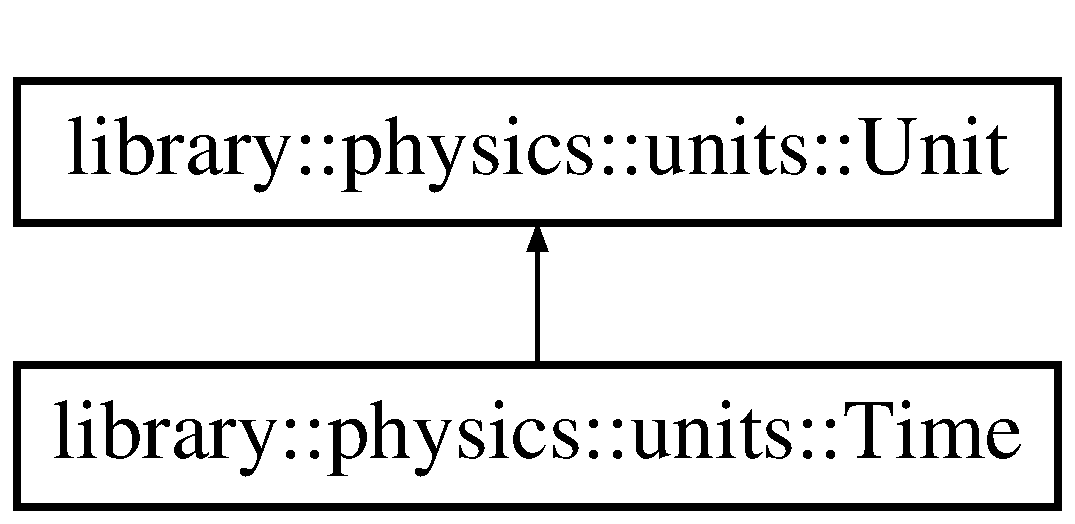
\includegraphics[height=2.000000cm]{classlibrary_1_1physics_1_1units_1_1_time}
\end{center}
\end{figure}
\subsection*{Public Types}
\begin{DoxyCompactItemize}
\item 
enum \hyperlink{classlibrary_1_1physics_1_1units_1_1_time_ab876a6a05c9a2f28905f2753bfd64109}{Unit} \{ \newline
\hyperlink{classlibrary_1_1physics_1_1units_1_1_time_ab876a6a05c9a2f28905f2753bfd64109aec0fc0100c4fc1ce4eea230c3dc10360}{Unit\+::\+Undefined}, 
\hyperlink{classlibrary_1_1physics_1_1units_1_1_time_ab876a6a05c9a2f28905f2753bfd64109a4146c294bcc82b1723c65bdc64b55089}{Unit\+::\+Nanosecond}, 
\hyperlink{classlibrary_1_1physics_1_1units_1_1_time_ab876a6a05c9a2f28905f2753bfd64109a1f14b3811ca5de688daa740d8471249e}{Unit\+::\+Microsecond}, 
\hyperlink{classlibrary_1_1physics_1_1units_1_1_time_ab876a6a05c9a2f28905f2753bfd64109a988bbeeb80e7e0a6b4651aab5a76b413}{Unit\+::\+Millisecond}, 
\newline
\hyperlink{classlibrary_1_1physics_1_1units_1_1_time_ab876a6a05c9a2f28905f2753bfd64109ac22cf8376b1893dcfcef0649fe1a7d87}{Unit\+::\+Second}, 
\hyperlink{classlibrary_1_1physics_1_1units_1_1_time_ab876a6a05c9a2f28905f2753bfd64109a62902641c38f3a4a8eb3212454360e24}{Unit\+::\+Minute}, 
\hyperlink{classlibrary_1_1physics_1_1units_1_1_time_ab876a6a05c9a2f28905f2753bfd64109ab55e509c697e4cca0e1d160a7806698f}{Unit\+::\+Hour}, 
\hyperlink{classlibrary_1_1physics_1_1units_1_1_time_ab876a6a05c9a2f28905f2753bfd64109a03727ac48595a24daed975559c944a44}{Unit\+::\+Day}, 
\newline
\hyperlink{classlibrary_1_1physics_1_1units_1_1_time_ab876a6a05c9a2f28905f2753bfd64109ad2ce009594dcc60befa6a4e6cbeb71fc}{Unit\+::\+Week}
 \}
\end{DoxyCompactItemize}
\subsection*{Public Member Functions}
\begin{DoxyCompactItemize}
\item 
\hyperlink{classlibrary_1_1physics_1_1units_1_1_time_a60e2228b16ea9156a4c5ede4d7b141e5}{Time} (const Real \&a\+Value, const \hyperlink{classlibrary_1_1physics_1_1units_1_1_time_ab876a6a05c9a2f28905f2753bfd64109}{Time\+::\+Unit} \&a\+Unit)
\begin{DoxyCompactList}\small\item\em Constructor. \end{DoxyCompactList}\item 
virtual bool \hyperlink{classlibrary_1_1physics_1_1units_1_1_time_ab62163386c3253277c5ba71782261cad}{is\+Defined} () const override
\item 
virtual String \hyperlink{classlibrary_1_1physics_1_1units_1_1_time_a6f56977493a45d334bb53bc4246888c4}{to\+String} (const Integer \&a\+Precision=Integer\+::\+Undefined()) const override
\end{DoxyCompactItemize}
\subsection*{Static Public Member Functions}
\begin{DoxyCompactItemize}
\item 
static \hyperlink{classlibrary_1_1physics_1_1units_1_1_time}{Time} \hyperlink{classlibrary_1_1physics_1_1units_1_1_time_a532c992968408dcb70f5ee94e672c595}{Undefined} ()
\item 
static String \hyperlink{classlibrary_1_1physics_1_1units_1_1_time_a413c7045742e568efc2e0e2b64eb6c86}{String\+From\+Unit} (const \hyperlink{classlibrary_1_1physics_1_1units_1_1_time_ab876a6a05c9a2f28905f2753bfd64109}{Time\+::\+Unit} \&a\+Unit)
\item 
static String \hyperlink{classlibrary_1_1physics_1_1units_1_1_time_aa48f07fb50e09cd22b9b6b7a83275f39}{Symbol\+From\+Unit} (const \hyperlink{classlibrary_1_1physics_1_1units_1_1_time_ab876a6a05c9a2f28905f2753bfd64109}{Time\+::\+Unit} \&a\+Unit)
\end{DoxyCompactItemize}


\subsection{Detailed Description}
\hyperlink{classlibrary_1_1physics_1_1units_1_1_time}{Time}. 

https\+://en.wikipedia.\+org/wiki/\+Unit\+\_\+of\+\_\+time 

\subsection{Member Enumeration Documentation}
\mbox{\Hypertarget{classlibrary_1_1physics_1_1units_1_1_time_ab876a6a05c9a2f28905f2753bfd64109}\label{classlibrary_1_1physics_1_1units_1_1_time_ab876a6a05c9a2f28905f2753bfd64109}} 
\index{library\+::physics\+::units\+::\+Time@{library\+::physics\+::units\+::\+Time}!Unit@{Unit}}
\index{Unit@{Unit}!library\+::physics\+::units\+::\+Time@{library\+::physics\+::units\+::\+Time}}
\subsubsection{\texorpdfstring{Unit}{Unit}}
{\footnotesize\ttfamily enum \hyperlink{classlibrary_1_1physics_1_1units_1_1_time_ab876a6a05c9a2f28905f2753bfd64109}{library\+::physics\+::units\+::\+Time\+::\+Unit}\hspace{0.3cm}{\ttfamily [strong]}}

\begin{DoxyEnumFields}{Enumerator}
\raisebox{\heightof{T}}[0pt][0pt]{\index{Undefined@{Undefined}!library\+::physics\+::units\+::\+Time@{library\+::physics\+::units\+::\+Time}}\index{library\+::physics\+::units\+::\+Time@{library\+::physics\+::units\+::\+Time}!Undefined@{Undefined}}}\mbox{\Hypertarget{classlibrary_1_1physics_1_1units_1_1_time_ab876a6a05c9a2f28905f2753bfd64109aec0fc0100c4fc1ce4eea230c3dc10360}\label{classlibrary_1_1physics_1_1units_1_1_time_ab876a6a05c9a2f28905f2753bfd64109aec0fc0100c4fc1ce4eea230c3dc10360}} 
Undefined&Undefined. \\
\hline

\raisebox{\heightof{T}}[0pt][0pt]{\index{Nanosecond@{Nanosecond}!library\+::physics\+::units\+::\+Time@{library\+::physics\+::units\+::\+Time}}\index{library\+::physics\+::units\+::\+Time@{library\+::physics\+::units\+::\+Time}!Nanosecond@{Nanosecond}}}\mbox{\Hypertarget{classlibrary_1_1physics_1_1units_1_1_time_ab876a6a05c9a2f28905f2753bfd64109a4146c294bcc82b1723c65bdc64b55089}\label{classlibrary_1_1physics_1_1units_1_1_time_ab876a6a05c9a2f28905f2753bfd64109a4146c294bcc82b1723c65bdc64b55089}} 
Nanosecond&Nanosecond. \\
\hline

\raisebox{\heightof{T}}[0pt][0pt]{\index{Microsecond@{Microsecond}!library\+::physics\+::units\+::\+Time@{library\+::physics\+::units\+::\+Time}}\index{library\+::physics\+::units\+::\+Time@{library\+::physics\+::units\+::\+Time}!Microsecond@{Microsecond}}}\mbox{\Hypertarget{classlibrary_1_1physics_1_1units_1_1_time_ab876a6a05c9a2f28905f2753bfd64109a1f14b3811ca5de688daa740d8471249e}\label{classlibrary_1_1physics_1_1units_1_1_time_ab876a6a05c9a2f28905f2753bfd64109a1f14b3811ca5de688daa740d8471249e}} 
Microsecond&Microsecond. \\
\hline

\raisebox{\heightof{T}}[0pt][0pt]{\index{Millisecond@{Millisecond}!library\+::physics\+::units\+::\+Time@{library\+::physics\+::units\+::\+Time}}\index{library\+::physics\+::units\+::\+Time@{library\+::physics\+::units\+::\+Time}!Millisecond@{Millisecond}}}\mbox{\Hypertarget{classlibrary_1_1physics_1_1units_1_1_time_ab876a6a05c9a2f28905f2753bfd64109a988bbeeb80e7e0a6b4651aab5a76b413}\label{classlibrary_1_1physics_1_1units_1_1_time_ab876a6a05c9a2f28905f2753bfd64109a988bbeeb80e7e0a6b4651aab5a76b413}} 
Millisecond&Millisecond. \\
\hline

\raisebox{\heightof{T}}[0pt][0pt]{\index{Second@{Second}!library\+::physics\+::units\+::\+Time@{library\+::physics\+::units\+::\+Time}}\index{library\+::physics\+::units\+::\+Time@{library\+::physics\+::units\+::\+Time}!Second@{Second}}}\mbox{\Hypertarget{classlibrary_1_1physics_1_1units_1_1_time_ab876a6a05c9a2f28905f2753bfd64109ac22cf8376b1893dcfcef0649fe1a7d87}\label{classlibrary_1_1physics_1_1units_1_1_time_ab876a6a05c9a2f28905f2753bfd64109ac22cf8376b1893dcfcef0649fe1a7d87}} 
Second&Second (SI) \\
\hline

\raisebox{\heightof{T}}[0pt][0pt]{\index{Minute@{Minute}!library\+::physics\+::units\+::\+Time@{library\+::physics\+::units\+::\+Time}}\index{library\+::physics\+::units\+::\+Time@{library\+::physics\+::units\+::\+Time}!Minute@{Minute}}}\mbox{\Hypertarget{classlibrary_1_1physics_1_1units_1_1_time_ab876a6a05c9a2f28905f2753bfd64109a62902641c38f3a4a8eb3212454360e24}\label{classlibrary_1_1physics_1_1units_1_1_time_ab876a6a05c9a2f28905f2753bfd64109a62902641c38f3a4a8eb3212454360e24}} 
Minute&Minute. \\
\hline

\raisebox{\heightof{T}}[0pt][0pt]{\index{Hour@{Hour}!library\+::physics\+::units\+::\+Time@{library\+::physics\+::units\+::\+Time}}\index{library\+::physics\+::units\+::\+Time@{library\+::physics\+::units\+::\+Time}!Hour@{Hour}}}\mbox{\Hypertarget{classlibrary_1_1physics_1_1units_1_1_time_ab876a6a05c9a2f28905f2753bfd64109ab55e509c697e4cca0e1d160a7806698f}\label{classlibrary_1_1physics_1_1units_1_1_time_ab876a6a05c9a2f28905f2753bfd64109ab55e509c697e4cca0e1d160a7806698f}} 
Hour&Hour. \\
\hline

\raisebox{\heightof{T}}[0pt][0pt]{\index{Day@{Day}!library\+::physics\+::units\+::\+Time@{library\+::physics\+::units\+::\+Time}}\index{library\+::physics\+::units\+::\+Time@{library\+::physics\+::units\+::\+Time}!Day@{Day}}}\mbox{\Hypertarget{classlibrary_1_1physics_1_1units_1_1_time_ab876a6a05c9a2f28905f2753bfd64109a03727ac48595a24daed975559c944a44}\label{classlibrary_1_1physics_1_1units_1_1_time_ab876a6a05c9a2f28905f2753bfd64109a03727ac48595a24daed975559c944a44}} 
Day&Day. \\
\hline

\raisebox{\heightof{T}}[0pt][0pt]{\index{Week@{Week}!library\+::physics\+::units\+::\+Time@{library\+::physics\+::units\+::\+Time}}\index{library\+::physics\+::units\+::\+Time@{library\+::physics\+::units\+::\+Time}!Week@{Week}}}\mbox{\Hypertarget{classlibrary_1_1physics_1_1units_1_1_time_ab876a6a05c9a2f28905f2753bfd64109ad2ce009594dcc60befa6a4e6cbeb71fc}\label{classlibrary_1_1physics_1_1units_1_1_time_ab876a6a05c9a2f28905f2753bfd64109ad2ce009594dcc60befa6a4e6cbeb71fc}} 
Week&Week. \\
\hline

\end{DoxyEnumFields}


\subsection{Constructor \& Destructor Documentation}
\mbox{\Hypertarget{classlibrary_1_1physics_1_1units_1_1_time_a60e2228b16ea9156a4c5ede4d7b141e5}\label{classlibrary_1_1physics_1_1units_1_1_time_a60e2228b16ea9156a4c5ede4d7b141e5}} 
\index{library\+::physics\+::units\+::\+Time@{library\+::physics\+::units\+::\+Time}!Time@{Time}}
\index{Time@{Time}!library\+::physics\+::units\+::\+Time@{library\+::physics\+::units\+::\+Time}}
\subsubsection{\texorpdfstring{Time()}{Time()}}
{\footnotesize\ttfamily library\+::physics\+::units\+::\+Time\+::\+Time (\begin{DoxyParamCaption}\item[{const Real \&}]{a\+Value,  }\item[{const \hyperlink{classlibrary_1_1physics_1_1units_1_1_time_ab876a6a05c9a2f28905f2753bfd64109}{Time\+::\+Unit} \&}]{a\+Unit }\end{DoxyParamCaption})}



Constructor. 


\begin{DoxyCode}
\hyperlink{classlibrary_1_1physics_1_1units_1_1_time_a60e2228b16ea9156a4c5ede4d7b141e5}{Time} time(1.0, \hyperlink{classlibrary_1_1physics_1_1units_1_1_time_ab876a6a05c9a2f28905f2753bfd64109ac22cf8376b1893dcfcef0649fe1a7d87}{Time::Unit::Second}) ;
\end{DoxyCode}



\begin{DoxyParams}[1]{Parameters}
\mbox{\tt in}  & {\em a\+Value} & A value \\
\hline
\mbox{\tt in}  & {\em a\+Unit} & A time unit \\
\hline
\end{DoxyParams}


\subsection{Member Function Documentation}
\mbox{\Hypertarget{classlibrary_1_1physics_1_1units_1_1_time_ab62163386c3253277c5ba71782261cad}\label{classlibrary_1_1physics_1_1units_1_1_time_ab62163386c3253277c5ba71782261cad}} 
\index{library\+::physics\+::units\+::\+Time@{library\+::physics\+::units\+::\+Time}!is\+Defined@{is\+Defined}}
\index{is\+Defined@{is\+Defined}!library\+::physics\+::units\+::\+Time@{library\+::physics\+::units\+::\+Time}}
\subsubsection{\texorpdfstring{is\+Defined()}{isDefined()}}
{\footnotesize\ttfamily bool library\+::physics\+::units\+::\+Time\+::is\+Defined (\begin{DoxyParamCaption}{ }\end{DoxyParamCaption}) const\hspace{0.3cm}{\ttfamily [override]}, {\ttfamily [virtual]}}



Reimplemented from \hyperlink{classlibrary_1_1physics_1_1units_1_1_unit_a5ce011c1ffa0fce4cf1f5d42ff06ee78}{library\+::physics\+::units\+::\+Unit}.

\mbox{\Hypertarget{classlibrary_1_1physics_1_1units_1_1_time_a413c7045742e568efc2e0e2b64eb6c86}\label{classlibrary_1_1physics_1_1units_1_1_time_a413c7045742e568efc2e0e2b64eb6c86}} 
\index{library\+::physics\+::units\+::\+Time@{library\+::physics\+::units\+::\+Time}!String\+From\+Unit@{String\+From\+Unit}}
\index{String\+From\+Unit@{String\+From\+Unit}!library\+::physics\+::units\+::\+Time@{library\+::physics\+::units\+::\+Time}}
\subsubsection{\texorpdfstring{String\+From\+Unit()}{StringFromUnit()}}
{\footnotesize\ttfamily String library\+::physics\+::units\+::\+Time\+::\+String\+From\+Unit (\begin{DoxyParamCaption}\item[{const \hyperlink{classlibrary_1_1physics_1_1units_1_1_time_ab876a6a05c9a2f28905f2753bfd64109}{Time\+::\+Unit} \&}]{a\+Unit }\end{DoxyParamCaption})\hspace{0.3cm}{\ttfamily [static]}}

\mbox{\Hypertarget{classlibrary_1_1physics_1_1units_1_1_time_aa48f07fb50e09cd22b9b6b7a83275f39}\label{classlibrary_1_1physics_1_1units_1_1_time_aa48f07fb50e09cd22b9b6b7a83275f39}} 
\index{library\+::physics\+::units\+::\+Time@{library\+::physics\+::units\+::\+Time}!Symbol\+From\+Unit@{Symbol\+From\+Unit}}
\index{Symbol\+From\+Unit@{Symbol\+From\+Unit}!library\+::physics\+::units\+::\+Time@{library\+::physics\+::units\+::\+Time}}
\subsubsection{\texorpdfstring{Symbol\+From\+Unit()}{SymbolFromUnit()}}
{\footnotesize\ttfamily String library\+::physics\+::units\+::\+Time\+::\+Symbol\+From\+Unit (\begin{DoxyParamCaption}\item[{const \hyperlink{classlibrary_1_1physics_1_1units_1_1_time_ab876a6a05c9a2f28905f2753bfd64109}{Time\+::\+Unit} \&}]{a\+Unit }\end{DoxyParamCaption})\hspace{0.3cm}{\ttfamily [static]}}

\mbox{\Hypertarget{classlibrary_1_1physics_1_1units_1_1_time_a6f56977493a45d334bb53bc4246888c4}\label{classlibrary_1_1physics_1_1units_1_1_time_a6f56977493a45d334bb53bc4246888c4}} 
\index{library\+::physics\+::units\+::\+Time@{library\+::physics\+::units\+::\+Time}!to\+String@{to\+String}}
\index{to\+String@{to\+String}!library\+::physics\+::units\+::\+Time@{library\+::physics\+::units\+::\+Time}}
\subsubsection{\texorpdfstring{to\+String()}{toString()}}
{\footnotesize\ttfamily String library\+::physics\+::units\+::\+Time\+::to\+String (\begin{DoxyParamCaption}\item[{const Integer \&}]{a\+Precision = {\ttfamily Integer\+:\+:Undefined()} }\end{DoxyParamCaption}) const\hspace{0.3cm}{\ttfamily [override]}, {\ttfamily [virtual]}}



Implements \hyperlink{classlibrary_1_1physics_1_1units_1_1_unit_aac05cb6ed1ea7c18c233a3381c81caf8}{library\+::physics\+::units\+::\+Unit}.

\mbox{\Hypertarget{classlibrary_1_1physics_1_1units_1_1_time_a532c992968408dcb70f5ee94e672c595}\label{classlibrary_1_1physics_1_1units_1_1_time_a532c992968408dcb70f5ee94e672c595}} 
\index{library\+::physics\+::units\+::\+Time@{library\+::physics\+::units\+::\+Time}!Undefined@{Undefined}}
\index{Undefined@{Undefined}!library\+::physics\+::units\+::\+Time@{library\+::physics\+::units\+::\+Time}}
\subsubsection{\texorpdfstring{Undefined()}{Undefined()}}
{\footnotesize\ttfamily \hyperlink{classlibrary_1_1physics_1_1units_1_1_time}{Time} library\+::physics\+::units\+::\+Time\+::\+Undefined (\begin{DoxyParamCaption}{ }\end{DoxyParamCaption})\hspace{0.3cm}{\ttfamily [static]}}



The documentation for this class was generated from the following files\+:\begin{DoxyCompactItemize}
\item 
include/\+Library/\+Physics/\+Units/\hyperlink{_units_2_time_8hpp}{Time.\+hpp}\item 
src/\+Library/\+Physics/\+Units/\hyperlink{_units_2_time_8cpp}{Time.\+cpp}\end{DoxyCompactItemize}

\hypertarget{classlibrary_1_1physics_1_1coord_1_1frame_1_1provider_1_1_t_i_r_f}{}\section{library\+:\+:physics\+:\+:coord\+:\+:frame\+:\+:provider\+:\+:T\+I\+RF Class Reference}
\label{classlibrary_1_1physics_1_1coord_1_1frame_1_1provider_1_1_t_i_r_f}\index{library\+::physics\+::coord\+::frame\+::provider\+::\+T\+I\+RF@{library\+::physics\+::coord\+::frame\+::provider\+::\+T\+I\+RF}}


Terrestrial Intermediate Reference \hyperlink{classlibrary_1_1physics_1_1coord_1_1_frame}{Frame} (\hyperlink{classlibrary_1_1physics_1_1coord_1_1frame_1_1provider_1_1_t_i_r_f}{T\+I\+RF}) provider.  




{\ttfamily \#include $<$T\+I\+R\+F.\+hpp$>$}

Inheritance diagram for library\+:\+:physics\+:\+:coord\+:\+:frame\+:\+:provider\+:\+:T\+I\+RF\+:\begin{figure}[H]
\begin{center}
\leavevmode
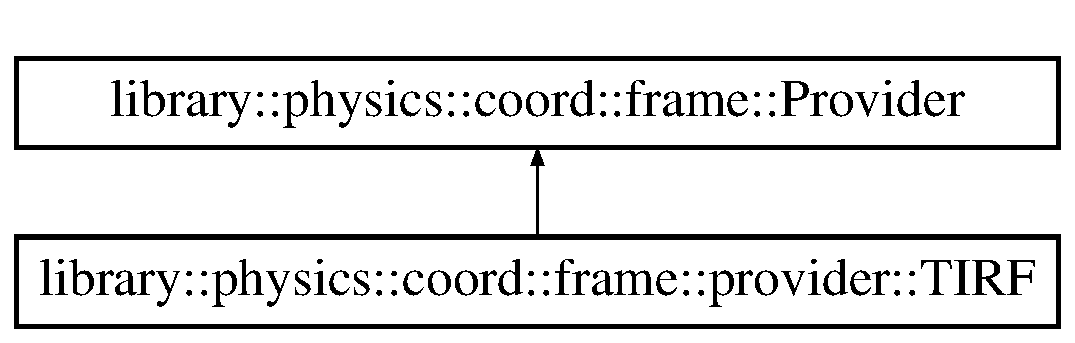
\includegraphics[height=2.000000cm]{classlibrary_1_1physics_1_1coord_1_1frame_1_1provider_1_1_t_i_r_f}
\end{center}
\end{figure}
\subsection*{Public Member Functions}
\begin{DoxyCompactItemize}
\item 
\hyperlink{classlibrary_1_1physics_1_1coord_1_1frame_1_1provider_1_1_t_i_r_f_af1a083499a1623494ae95abd5adbfb93}{T\+I\+RF} ()
\item 
virtual \hyperlink{classlibrary_1_1physics_1_1coord_1_1frame_1_1provider_1_1_t_i_r_f_ade20a8def3caccb02466e2349e0924e5}{$\sim$\+T\+I\+RF} () override
\item 
virtual \hyperlink{classlibrary_1_1physics_1_1coord_1_1frame_1_1provider_1_1_t_i_r_f}{T\+I\+RF} $\ast$ \hyperlink{classlibrary_1_1physics_1_1coord_1_1frame_1_1provider_1_1_t_i_r_f_a48ef3f686e9bcc744a5e3d1fa1779ab6}{clone} () const override
\item 
virtual bool \hyperlink{classlibrary_1_1physics_1_1coord_1_1frame_1_1provider_1_1_t_i_r_f_a3656639fda8a7b991335752559d7594b}{is\+Defined} () const override
\item 
virtual \hyperlink{classlibrary_1_1physics_1_1coord_1_1_transform}{Transform} \hyperlink{classlibrary_1_1physics_1_1coord_1_1frame_1_1provider_1_1_t_i_r_f_a89eea1b9ff4b38937bf51099e8dd6333}{get\+Transform\+At} (const \hyperlink{classlibrary_1_1physics_1_1time_1_1_instant}{Instant} \&an\+Instant) const override
\end{DoxyCompactItemize}


\subsection{Detailed Description}
Terrestrial Intermediate Reference \hyperlink{classlibrary_1_1physics_1_1coord_1_1_frame}{Frame} (\hyperlink{classlibrary_1_1physics_1_1coord_1_1frame_1_1provider_1_1_t_i_r_f}{T\+I\+RF}) provider. 

Earth rotation angle

https\+://www.iers.\+org/\+Shared\+Docs/\+Publikationen/\+E\+N/\+I\+E\+R\+S/\+Publications/tn/\+Techn\+Note36/tn36\+\_\+174.pdf?\+\_\+\+\_\+blob=publication\+File\&v=1 

\subsection{Constructor \& Destructor Documentation}
\mbox{\Hypertarget{classlibrary_1_1physics_1_1coord_1_1frame_1_1provider_1_1_t_i_r_f_af1a083499a1623494ae95abd5adbfb93}\label{classlibrary_1_1physics_1_1coord_1_1frame_1_1provider_1_1_t_i_r_f_af1a083499a1623494ae95abd5adbfb93}} 
\index{library\+::physics\+::coord\+::frame\+::provider\+::\+T\+I\+RF@{library\+::physics\+::coord\+::frame\+::provider\+::\+T\+I\+RF}!T\+I\+RF@{T\+I\+RF}}
\index{T\+I\+RF@{T\+I\+RF}!library\+::physics\+::coord\+::frame\+::provider\+::\+T\+I\+RF@{library\+::physics\+::coord\+::frame\+::provider\+::\+T\+I\+RF}}
\subsubsection{\texorpdfstring{T\+I\+R\+F()}{TIRF()}}
{\footnotesize\ttfamily library\+::physics\+::coord\+::frame\+::provider\+::\+T\+I\+R\+F\+::\+T\+I\+RF (\begin{DoxyParamCaption}{ }\end{DoxyParamCaption})}

\mbox{\Hypertarget{classlibrary_1_1physics_1_1coord_1_1frame_1_1provider_1_1_t_i_r_f_ade20a8def3caccb02466e2349e0924e5}\label{classlibrary_1_1physics_1_1coord_1_1frame_1_1provider_1_1_t_i_r_f_ade20a8def3caccb02466e2349e0924e5}} 
\index{library\+::physics\+::coord\+::frame\+::provider\+::\+T\+I\+RF@{library\+::physics\+::coord\+::frame\+::provider\+::\+T\+I\+RF}!````~T\+I\+RF@{$\sim$\+T\+I\+RF}}
\index{````~T\+I\+RF@{$\sim$\+T\+I\+RF}!library\+::physics\+::coord\+::frame\+::provider\+::\+T\+I\+RF@{library\+::physics\+::coord\+::frame\+::provider\+::\+T\+I\+RF}}
\subsubsection{\texorpdfstring{$\sim$\+T\+I\+R\+F()}{~TIRF()}}
{\footnotesize\ttfamily library\+::physics\+::coord\+::frame\+::provider\+::\+T\+I\+R\+F\+::$\sim$\+T\+I\+RF (\begin{DoxyParamCaption}{ }\end{DoxyParamCaption})\hspace{0.3cm}{\ttfamily [override]}, {\ttfamily [virtual]}}



\subsection{Member Function Documentation}
\mbox{\Hypertarget{classlibrary_1_1physics_1_1coord_1_1frame_1_1provider_1_1_t_i_r_f_a48ef3f686e9bcc744a5e3d1fa1779ab6}\label{classlibrary_1_1physics_1_1coord_1_1frame_1_1provider_1_1_t_i_r_f_a48ef3f686e9bcc744a5e3d1fa1779ab6}} 
\index{library\+::physics\+::coord\+::frame\+::provider\+::\+T\+I\+RF@{library\+::physics\+::coord\+::frame\+::provider\+::\+T\+I\+RF}!clone@{clone}}
\index{clone@{clone}!library\+::physics\+::coord\+::frame\+::provider\+::\+T\+I\+RF@{library\+::physics\+::coord\+::frame\+::provider\+::\+T\+I\+RF}}
\subsubsection{\texorpdfstring{clone()}{clone()}}
{\footnotesize\ttfamily \hyperlink{classlibrary_1_1physics_1_1coord_1_1frame_1_1provider_1_1_t_i_r_f}{T\+I\+RF} $\ast$ library\+::physics\+::coord\+::frame\+::provider\+::\+T\+I\+R\+F\+::clone (\begin{DoxyParamCaption}{ }\end{DoxyParamCaption}) const\hspace{0.3cm}{\ttfamily [override]}, {\ttfamily [virtual]}}



Implements \hyperlink{classlibrary_1_1physics_1_1coord_1_1frame_1_1_provider_ab8eee40c8ef4aee0b57bedf458f4934e}{library\+::physics\+::coord\+::frame\+::\+Provider}.

\mbox{\Hypertarget{classlibrary_1_1physics_1_1coord_1_1frame_1_1provider_1_1_t_i_r_f_a89eea1b9ff4b38937bf51099e8dd6333}\label{classlibrary_1_1physics_1_1coord_1_1frame_1_1provider_1_1_t_i_r_f_a89eea1b9ff4b38937bf51099e8dd6333}} 
\index{library\+::physics\+::coord\+::frame\+::provider\+::\+T\+I\+RF@{library\+::physics\+::coord\+::frame\+::provider\+::\+T\+I\+RF}!get\+Transform\+At@{get\+Transform\+At}}
\index{get\+Transform\+At@{get\+Transform\+At}!library\+::physics\+::coord\+::frame\+::provider\+::\+T\+I\+RF@{library\+::physics\+::coord\+::frame\+::provider\+::\+T\+I\+RF}}
\subsubsection{\texorpdfstring{get\+Transform\+At()}{getTransformAt()}}
{\footnotesize\ttfamily \hyperlink{classlibrary_1_1physics_1_1coord_1_1_transform}{Transform} library\+::physics\+::coord\+::frame\+::provider\+::\+T\+I\+R\+F\+::get\+Transform\+At (\begin{DoxyParamCaption}\item[{const \hyperlink{classlibrary_1_1physics_1_1time_1_1_instant}{Instant} \&}]{an\+Instant }\end{DoxyParamCaption}) const\hspace{0.3cm}{\ttfamily [override]}, {\ttfamily [virtual]}}



Implements \hyperlink{classlibrary_1_1physics_1_1coord_1_1frame_1_1_provider_a796fd2dd337f1304a0e9acf573ce2550}{library\+::physics\+::coord\+::frame\+::\+Provider}.

\mbox{\Hypertarget{classlibrary_1_1physics_1_1coord_1_1frame_1_1provider_1_1_t_i_r_f_a3656639fda8a7b991335752559d7594b}\label{classlibrary_1_1physics_1_1coord_1_1frame_1_1provider_1_1_t_i_r_f_a3656639fda8a7b991335752559d7594b}} 
\index{library\+::physics\+::coord\+::frame\+::provider\+::\+T\+I\+RF@{library\+::physics\+::coord\+::frame\+::provider\+::\+T\+I\+RF}!is\+Defined@{is\+Defined}}
\index{is\+Defined@{is\+Defined}!library\+::physics\+::coord\+::frame\+::provider\+::\+T\+I\+RF@{library\+::physics\+::coord\+::frame\+::provider\+::\+T\+I\+RF}}
\subsubsection{\texorpdfstring{is\+Defined()}{isDefined()}}
{\footnotesize\ttfamily bool library\+::physics\+::coord\+::frame\+::provider\+::\+T\+I\+R\+F\+::is\+Defined (\begin{DoxyParamCaption}{ }\end{DoxyParamCaption}) const\hspace{0.3cm}{\ttfamily [override]}, {\ttfamily [virtual]}}



Implements \hyperlink{classlibrary_1_1physics_1_1coord_1_1frame_1_1_provider_ae7cd093febf2b20f71400f9f79442774}{library\+::physics\+::coord\+::frame\+::\+Provider}.



The documentation for this class was generated from the following files\+:\begin{DoxyCompactItemize}
\item 
include/\+Library/\+Physics/\+Coordinate/\+Frame/\+Providers/\hyperlink{_t_i_r_f_8hpp}{T\+I\+R\+F.\+hpp}\item 
src/\+Library/\+Physics/\+Coordinate/\+Frame/\+Providers/\hyperlink{_t_i_r_f_8cpp}{T\+I\+R\+F.\+cpp}\end{DoxyCompactItemize}

\hypertarget{classlibrary_1_1physics_1_1coord_1_1_transform}{}\section{library\+:\+:physics\+:\+:coord\+:\+:Transform Class Reference}
\label{classlibrary_1_1physics_1_1coord_1_1_transform}\index{library\+::physics\+::coord\+::\+Transform@{library\+::physics\+::coord\+::\+Transform}}


\hyperlink{classlibrary_1_1physics_1_1coord_1_1_transform}{Transform}.  




{\ttfamily \#include $<$Transform.\+hpp$>$}

\subsection*{Public Types}
\begin{DoxyCompactItemize}
\item 
enum \hyperlink{classlibrary_1_1physics_1_1coord_1_1_transform_a4f19d7d232ce1fda0dcee16e4157db2c}{Type} \{ \hyperlink{classlibrary_1_1physics_1_1coord_1_1_transform_a4f19d7d232ce1fda0dcee16e4157db2caec0fc0100c4fc1ce4eea230c3dc10360}{Type\+::\+Undefined}, 
\hyperlink{classlibrary_1_1physics_1_1coord_1_1_transform_a4f19d7d232ce1fda0dcee16e4157db2ca4d3d769b812b6faa6b76e1a8abaece2d}{Type\+::\+Active}, 
\hyperlink{classlibrary_1_1physics_1_1coord_1_1_transform_a4f19d7d232ce1fda0dcee16e4157db2caf80bc338b6146b566004a046f8137c85}{Type\+::\+Passive}
 \}
\end{DoxyCompactItemize}
\subsection*{Public Member Functions}
\begin{DoxyCompactItemize}
\item 
\hyperlink{classlibrary_1_1physics_1_1coord_1_1_transform_ac4b91f8f159f3319174e091cf6103cf9}{Transform} (const \hyperlink{classlibrary_1_1physics_1_1time_1_1_instant}{Instant} \&an\+Instant, const Vector3d \&a\+Translation, const Vector3d \&a\+Velocity, const Quaternion \&an\+Orientation, const Vector3d \&an\+Angular\+Velocity, const \hyperlink{classlibrary_1_1physics_1_1coord_1_1_transform_a4f19d7d232ce1fda0dcee16e4157db2c}{Transform\+::\+Type} \&a\+Type)
\item 
bool \hyperlink{classlibrary_1_1physics_1_1coord_1_1_transform_a7fd14bfb2953041a020521c3b34c5309}{operator==} (const \hyperlink{classlibrary_1_1physics_1_1coord_1_1_transform}{Transform} \&a\+Transform) const
\item 
bool \hyperlink{classlibrary_1_1physics_1_1coord_1_1_transform_a0481b3053d7dfb4a3cfc7ced3a13dc68}{operator!=} (const \hyperlink{classlibrary_1_1physics_1_1coord_1_1_transform}{Transform} \&a\+Transform) const
\item 
\hyperlink{classlibrary_1_1physics_1_1coord_1_1_transform}{Transform} \hyperlink{classlibrary_1_1physics_1_1coord_1_1_transform_a61e4d3b1cbbebb7e882f421d2f732d64}{operator$\ast$} (const \hyperlink{classlibrary_1_1physics_1_1coord_1_1_transform}{Transform} \&a\+Transform) const
\item 
\hyperlink{classlibrary_1_1physics_1_1coord_1_1_transform}{Transform} \& \hyperlink{classlibrary_1_1physics_1_1coord_1_1_transform_af0e36a56b799db736bd4e2228a48a8e6}{operator$\ast$=} (const \hyperlink{classlibrary_1_1physics_1_1coord_1_1_transform}{Transform} \&a\+Transform)
\item 
bool \hyperlink{classlibrary_1_1physics_1_1coord_1_1_transform_a782bf485d01d3ff9b38cabe94ff9406f}{is\+Defined} () const
\item 
const \hyperlink{classlibrary_1_1physics_1_1time_1_1_instant}{Instant} \& \hyperlink{classlibrary_1_1physics_1_1coord_1_1_transform_aaa29bb2f60c383af21967078ed90fa6e}{access\+Instant} () const
\item 
const Vector3d \& \hyperlink{classlibrary_1_1physics_1_1coord_1_1_transform_a18fcdf0a8123a3e6a2551b93830fb909}{access\+Translation} () const
\item 
const Vector3d \& \hyperlink{classlibrary_1_1physics_1_1coord_1_1_transform_a376d079de305b16e05251bfe84ca2199}{access\+Velocity} () const
\item 
const Quaternion \& \hyperlink{classlibrary_1_1physics_1_1coord_1_1_transform_aac7f3bf9570d378aab4e9c62f3478560}{access\+Orientation} () const
\item 
const Vector3d \& \hyperlink{classlibrary_1_1physics_1_1coord_1_1_transform_a0e7dc9e3c40a5e3b836ccb10e250d207}{access\+Angular\+Velocity} () const
\item 
\hyperlink{classlibrary_1_1physics_1_1time_1_1_instant}{Instant} \hyperlink{classlibrary_1_1physics_1_1coord_1_1_transform_a674c8ac4676d07aa641b85e049233838}{get\+Instant} () const
\item 
Vector3d \hyperlink{classlibrary_1_1physics_1_1coord_1_1_transform_a9cdc57080aff638c321de68564bf913b}{get\+Translation} () const
\item 
Vector3d \hyperlink{classlibrary_1_1physics_1_1coord_1_1_transform_aa5d6b48208919b34cdafb9ea56aaef12}{get\+Velocity} () const
\item 
Quaternion \hyperlink{classlibrary_1_1physics_1_1coord_1_1_transform_a401692acc8f82e03373feed88c6d45b2}{get\+Orientation} () const
\item 
Vector3d \hyperlink{classlibrary_1_1physics_1_1coord_1_1_transform_a06059603f73cc34da4cd1d731e1c09fa}{get\+Angular\+Velocity} () const
\item 
\hyperlink{classlibrary_1_1physics_1_1coord_1_1_transform}{Transform} \hyperlink{classlibrary_1_1physics_1_1coord_1_1_transform_a4d2cbec2ec7dadd2b4f8dd1d4184b692}{get\+Inverse} () const
\item 
Vector3d \hyperlink{classlibrary_1_1physics_1_1coord_1_1_transform_ae55f2f7fc9769d42ac31f9e5fd0ddfe5}{apply\+To\+Position} (const Vector3d \&a\+Position) const
\item 
Vector3d \hyperlink{classlibrary_1_1physics_1_1coord_1_1_transform_a017c1ec77f5ddda3f7d93dd63a9a6d3f}{apply\+To\+Velocity} (const Vector3d \&a\+Position, const Vector3d \&a\+Velocity) const
\item 
Vector3d \hyperlink{classlibrary_1_1physics_1_1coord_1_1_transform_a0709a5af7a97adbda05a24b9d4ad677d}{apply\+To\+Vector} (const Vector3d \&a\+Vector) const
\end{DoxyCompactItemize}
\subsection*{Static Public Member Functions}
\begin{DoxyCompactItemize}
\item 
static \hyperlink{classlibrary_1_1physics_1_1coord_1_1_transform}{Transform} \hyperlink{classlibrary_1_1physics_1_1coord_1_1_transform_ac346b5703e94945a10ab222bf38d2a08}{Undefined} ()
\item 
static \hyperlink{classlibrary_1_1physics_1_1coord_1_1_transform}{Transform} \hyperlink{classlibrary_1_1physics_1_1coord_1_1_transform_a941cf2c273c2c95d0a43e1050e35d537}{Identity} (const \hyperlink{classlibrary_1_1physics_1_1time_1_1_instant}{Instant} \&an\+Instant)
\item 
static \hyperlink{classlibrary_1_1physics_1_1coord_1_1_transform}{Transform} \hyperlink{classlibrary_1_1physics_1_1coord_1_1_transform_aa82ab1a4be06a10e7c8f004062fcc35d}{Active} (const \hyperlink{classlibrary_1_1physics_1_1time_1_1_instant}{Instant} \&an\+Instant, const Vector3d \&a\+Translation, const Vector3d \&a\+Velocity, const Quaternion \&an\+Orientation, const Vector3d \&an\+Angular\+Velocity)
\item 
static \hyperlink{classlibrary_1_1physics_1_1coord_1_1_transform}{Transform} \hyperlink{classlibrary_1_1physics_1_1coord_1_1_transform_ac8d745aa497d7713a19aa8652acb02c6}{Passive} (const \hyperlink{classlibrary_1_1physics_1_1time_1_1_instant}{Instant} \&an\+Instant, const Vector3d \&a\+Translation, const Vector3d \&a\+Velocity, const Quaternion \&an\+Orientation, const Vector3d \&an\+Angular\+Velocity)
\end{DoxyCompactItemize}
\subsection*{Friends}
\begin{DoxyCompactItemize}
\item 
std\+::ostream \& \hyperlink{classlibrary_1_1physics_1_1coord_1_1_transform_ae46ab7a297c23b757fd6f41bf30c4054}{operator$<$$<$} (std\+::ostream \&an\+Output\+Stream, const \hyperlink{classlibrary_1_1physics_1_1coord_1_1_transform}{Transform} \&a\+Transform)
\end{DoxyCompactItemize}


\subsection{Detailed Description}
\hyperlink{classlibrary_1_1physics_1_1coord_1_1_transform}{Transform}. 

Passive transformation

https\+://en.wikipedia.\+org/wiki/\+Active\+\_\+and\+\_\+passive\+\_\+transformation https\+://core.ac.\+uk/download/pdf/77055186.pdf 

\subsection{Member Enumeration Documentation}
\mbox{\Hypertarget{classlibrary_1_1physics_1_1coord_1_1_transform_a4f19d7d232ce1fda0dcee16e4157db2c}\label{classlibrary_1_1physics_1_1coord_1_1_transform_a4f19d7d232ce1fda0dcee16e4157db2c}} 
\index{library\+::physics\+::coord\+::\+Transform@{library\+::physics\+::coord\+::\+Transform}!Type@{Type}}
\index{Type@{Type}!library\+::physics\+::coord\+::\+Transform@{library\+::physics\+::coord\+::\+Transform}}
\subsubsection{\texorpdfstring{Type}{Type}}
{\footnotesize\ttfamily enum \hyperlink{classlibrary_1_1physics_1_1coord_1_1_transform_a4f19d7d232ce1fda0dcee16e4157db2c}{library\+::physics\+::coord\+::\+Transform\+::\+Type}\hspace{0.3cm}{\ttfamily [strong]}}

\begin{DoxyEnumFields}{Enumerator}
\raisebox{\heightof{T}}[0pt][0pt]{\index{Undefined@{Undefined}!library\+::physics\+::coord\+::\+Transform@{library\+::physics\+::coord\+::\+Transform}}\index{library\+::physics\+::coord\+::\+Transform@{library\+::physics\+::coord\+::\+Transform}!Undefined@{Undefined}}}\mbox{\Hypertarget{classlibrary_1_1physics_1_1coord_1_1_transform_a4f19d7d232ce1fda0dcee16e4157db2caec0fc0100c4fc1ce4eea230c3dc10360}\label{classlibrary_1_1physics_1_1coord_1_1_transform_a4f19d7d232ce1fda0dcee16e4157db2caec0fc0100c4fc1ce4eea230c3dc10360}} 
Undefined&\\
\hline

\raisebox{\heightof{T}}[0pt][0pt]{\index{Active@{Active}!library\+::physics\+::coord\+::\+Transform@{library\+::physics\+::coord\+::\+Transform}}\index{library\+::physics\+::coord\+::\+Transform@{library\+::physics\+::coord\+::\+Transform}!Active@{Active}}}\mbox{\Hypertarget{classlibrary_1_1physics_1_1coord_1_1_transform_a4f19d7d232ce1fda0dcee16e4157db2ca4d3d769b812b6faa6b76e1a8abaece2d}\label{classlibrary_1_1physics_1_1coord_1_1_transform_a4f19d7d232ce1fda0dcee16e4157db2ca4d3d769b812b6faa6b76e1a8abaece2d}} 
Active&\\
\hline

\raisebox{\heightof{T}}[0pt][0pt]{\index{Passive@{Passive}!library\+::physics\+::coord\+::\+Transform@{library\+::physics\+::coord\+::\+Transform}}\index{library\+::physics\+::coord\+::\+Transform@{library\+::physics\+::coord\+::\+Transform}!Passive@{Passive}}}\mbox{\Hypertarget{classlibrary_1_1physics_1_1coord_1_1_transform_a4f19d7d232ce1fda0dcee16e4157db2caf80bc338b6146b566004a046f8137c85}\label{classlibrary_1_1physics_1_1coord_1_1_transform_a4f19d7d232ce1fda0dcee16e4157db2caf80bc338b6146b566004a046f8137c85}} 
Passive&\\
\hline

\end{DoxyEnumFields}


\subsection{Constructor \& Destructor Documentation}
\mbox{\Hypertarget{classlibrary_1_1physics_1_1coord_1_1_transform_ac4b91f8f159f3319174e091cf6103cf9}\label{classlibrary_1_1physics_1_1coord_1_1_transform_ac4b91f8f159f3319174e091cf6103cf9}} 
\index{library\+::physics\+::coord\+::\+Transform@{library\+::physics\+::coord\+::\+Transform}!Transform@{Transform}}
\index{Transform@{Transform}!library\+::physics\+::coord\+::\+Transform@{library\+::physics\+::coord\+::\+Transform}}
\subsubsection{\texorpdfstring{Transform()}{Transform()}}
{\footnotesize\ttfamily library\+::physics\+::coord\+::\+Transform\+::\+Transform (\begin{DoxyParamCaption}\item[{const \hyperlink{classlibrary_1_1physics_1_1time_1_1_instant}{Instant} \&}]{an\+Instant,  }\item[{const Vector3d \&}]{a\+Translation,  }\item[{const Vector3d \&}]{a\+Velocity,  }\item[{const Quaternion \&}]{an\+Orientation,  }\item[{const Vector3d \&}]{an\+Angular\+Velocity,  }\item[{const \hyperlink{classlibrary_1_1physics_1_1coord_1_1_transform_a4f19d7d232ce1fda0dcee16e4157db2c}{Transform\+::\+Type} \&}]{a\+Type }\end{DoxyParamCaption})}



\subsection{Member Function Documentation}
\mbox{\Hypertarget{classlibrary_1_1physics_1_1coord_1_1_transform_a0e7dc9e3c40a5e3b836ccb10e250d207}\label{classlibrary_1_1physics_1_1coord_1_1_transform_a0e7dc9e3c40a5e3b836ccb10e250d207}} 
\index{library\+::physics\+::coord\+::\+Transform@{library\+::physics\+::coord\+::\+Transform}!access\+Angular\+Velocity@{access\+Angular\+Velocity}}
\index{access\+Angular\+Velocity@{access\+Angular\+Velocity}!library\+::physics\+::coord\+::\+Transform@{library\+::physics\+::coord\+::\+Transform}}
\subsubsection{\texorpdfstring{access\+Angular\+Velocity()}{accessAngularVelocity()}}
{\footnotesize\ttfamily const Vector3d \& library\+::physics\+::coord\+::\+Transform\+::access\+Angular\+Velocity (\begin{DoxyParamCaption}{ }\end{DoxyParamCaption}) const}

\mbox{\Hypertarget{classlibrary_1_1physics_1_1coord_1_1_transform_aaa29bb2f60c383af21967078ed90fa6e}\label{classlibrary_1_1physics_1_1coord_1_1_transform_aaa29bb2f60c383af21967078ed90fa6e}} 
\index{library\+::physics\+::coord\+::\+Transform@{library\+::physics\+::coord\+::\+Transform}!access\+Instant@{access\+Instant}}
\index{access\+Instant@{access\+Instant}!library\+::physics\+::coord\+::\+Transform@{library\+::physics\+::coord\+::\+Transform}}
\subsubsection{\texorpdfstring{access\+Instant()}{accessInstant()}}
{\footnotesize\ttfamily const \hyperlink{classlibrary_1_1physics_1_1time_1_1_instant}{Instant} \& library\+::physics\+::coord\+::\+Transform\+::access\+Instant (\begin{DoxyParamCaption}{ }\end{DoxyParamCaption}) const}

\mbox{\Hypertarget{classlibrary_1_1physics_1_1coord_1_1_transform_aac7f3bf9570d378aab4e9c62f3478560}\label{classlibrary_1_1physics_1_1coord_1_1_transform_aac7f3bf9570d378aab4e9c62f3478560}} 
\index{library\+::physics\+::coord\+::\+Transform@{library\+::physics\+::coord\+::\+Transform}!access\+Orientation@{access\+Orientation}}
\index{access\+Orientation@{access\+Orientation}!library\+::physics\+::coord\+::\+Transform@{library\+::physics\+::coord\+::\+Transform}}
\subsubsection{\texorpdfstring{access\+Orientation()}{accessOrientation()}}
{\footnotesize\ttfamily const Quaternion \& library\+::physics\+::coord\+::\+Transform\+::access\+Orientation (\begin{DoxyParamCaption}{ }\end{DoxyParamCaption}) const}

\mbox{\Hypertarget{classlibrary_1_1physics_1_1coord_1_1_transform_a18fcdf0a8123a3e6a2551b93830fb909}\label{classlibrary_1_1physics_1_1coord_1_1_transform_a18fcdf0a8123a3e6a2551b93830fb909}} 
\index{library\+::physics\+::coord\+::\+Transform@{library\+::physics\+::coord\+::\+Transform}!access\+Translation@{access\+Translation}}
\index{access\+Translation@{access\+Translation}!library\+::physics\+::coord\+::\+Transform@{library\+::physics\+::coord\+::\+Transform}}
\subsubsection{\texorpdfstring{access\+Translation()}{accessTranslation()}}
{\footnotesize\ttfamily const Vector3d \& library\+::physics\+::coord\+::\+Transform\+::access\+Translation (\begin{DoxyParamCaption}{ }\end{DoxyParamCaption}) const}

\mbox{\Hypertarget{classlibrary_1_1physics_1_1coord_1_1_transform_a376d079de305b16e05251bfe84ca2199}\label{classlibrary_1_1physics_1_1coord_1_1_transform_a376d079de305b16e05251bfe84ca2199}} 
\index{library\+::physics\+::coord\+::\+Transform@{library\+::physics\+::coord\+::\+Transform}!access\+Velocity@{access\+Velocity}}
\index{access\+Velocity@{access\+Velocity}!library\+::physics\+::coord\+::\+Transform@{library\+::physics\+::coord\+::\+Transform}}
\subsubsection{\texorpdfstring{access\+Velocity()}{accessVelocity()}}
{\footnotesize\ttfamily const Vector3d \& library\+::physics\+::coord\+::\+Transform\+::access\+Velocity (\begin{DoxyParamCaption}{ }\end{DoxyParamCaption}) const}

\mbox{\Hypertarget{classlibrary_1_1physics_1_1coord_1_1_transform_aa82ab1a4be06a10e7c8f004062fcc35d}\label{classlibrary_1_1physics_1_1coord_1_1_transform_aa82ab1a4be06a10e7c8f004062fcc35d}} 
\index{library\+::physics\+::coord\+::\+Transform@{library\+::physics\+::coord\+::\+Transform}!Active@{Active}}
\index{Active@{Active}!library\+::physics\+::coord\+::\+Transform@{library\+::physics\+::coord\+::\+Transform}}
\subsubsection{\texorpdfstring{Active()}{Active()}}
{\footnotesize\ttfamily \hyperlink{classlibrary_1_1physics_1_1coord_1_1_transform}{Transform} library\+::physics\+::coord\+::\+Transform\+::\+Active (\begin{DoxyParamCaption}\item[{const \hyperlink{classlibrary_1_1physics_1_1time_1_1_instant}{Instant} \&}]{an\+Instant,  }\item[{const Vector3d \&}]{a\+Translation,  }\item[{const Vector3d \&}]{a\+Velocity,  }\item[{const Quaternion \&}]{an\+Orientation,  }\item[{const Vector3d \&}]{an\+Angular\+Velocity }\end{DoxyParamCaption})\hspace{0.3cm}{\ttfamily [static]}}

\mbox{\Hypertarget{classlibrary_1_1physics_1_1coord_1_1_transform_ae55f2f7fc9769d42ac31f9e5fd0ddfe5}\label{classlibrary_1_1physics_1_1coord_1_1_transform_ae55f2f7fc9769d42ac31f9e5fd0ddfe5}} 
\index{library\+::physics\+::coord\+::\+Transform@{library\+::physics\+::coord\+::\+Transform}!apply\+To\+Position@{apply\+To\+Position}}
\index{apply\+To\+Position@{apply\+To\+Position}!library\+::physics\+::coord\+::\+Transform@{library\+::physics\+::coord\+::\+Transform}}
\subsubsection{\texorpdfstring{apply\+To\+Position()}{applyToPosition()}}
{\footnotesize\ttfamily Vector3d library\+::physics\+::coord\+::\+Transform\+::apply\+To\+Position (\begin{DoxyParamCaption}\item[{const Vector3d \&}]{a\+Position }\end{DoxyParamCaption}) const}

\mbox{\Hypertarget{classlibrary_1_1physics_1_1coord_1_1_transform_a0709a5af7a97adbda05a24b9d4ad677d}\label{classlibrary_1_1physics_1_1coord_1_1_transform_a0709a5af7a97adbda05a24b9d4ad677d}} 
\index{library\+::physics\+::coord\+::\+Transform@{library\+::physics\+::coord\+::\+Transform}!apply\+To\+Vector@{apply\+To\+Vector}}
\index{apply\+To\+Vector@{apply\+To\+Vector}!library\+::physics\+::coord\+::\+Transform@{library\+::physics\+::coord\+::\+Transform}}
\subsubsection{\texorpdfstring{apply\+To\+Vector()}{applyToVector()}}
{\footnotesize\ttfamily Vector3d library\+::physics\+::coord\+::\+Transform\+::apply\+To\+Vector (\begin{DoxyParamCaption}\item[{const Vector3d \&}]{a\+Vector }\end{DoxyParamCaption}) const}

\mbox{\Hypertarget{classlibrary_1_1physics_1_1coord_1_1_transform_a017c1ec77f5ddda3f7d93dd63a9a6d3f}\label{classlibrary_1_1physics_1_1coord_1_1_transform_a017c1ec77f5ddda3f7d93dd63a9a6d3f}} 
\index{library\+::physics\+::coord\+::\+Transform@{library\+::physics\+::coord\+::\+Transform}!apply\+To\+Velocity@{apply\+To\+Velocity}}
\index{apply\+To\+Velocity@{apply\+To\+Velocity}!library\+::physics\+::coord\+::\+Transform@{library\+::physics\+::coord\+::\+Transform}}
\subsubsection{\texorpdfstring{apply\+To\+Velocity()}{applyToVelocity()}}
{\footnotesize\ttfamily Vector3d library\+::physics\+::coord\+::\+Transform\+::apply\+To\+Velocity (\begin{DoxyParamCaption}\item[{const Vector3d \&}]{a\+Position,  }\item[{const Vector3d \&}]{a\+Velocity }\end{DoxyParamCaption}) const}

\mbox{\Hypertarget{classlibrary_1_1physics_1_1coord_1_1_transform_a06059603f73cc34da4cd1d731e1c09fa}\label{classlibrary_1_1physics_1_1coord_1_1_transform_a06059603f73cc34da4cd1d731e1c09fa}} 
\index{library\+::physics\+::coord\+::\+Transform@{library\+::physics\+::coord\+::\+Transform}!get\+Angular\+Velocity@{get\+Angular\+Velocity}}
\index{get\+Angular\+Velocity@{get\+Angular\+Velocity}!library\+::physics\+::coord\+::\+Transform@{library\+::physics\+::coord\+::\+Transform}}
\subsubsection{\texorpdfstring{get\+Angular\+Velocity()}{getAngularVelocity()}}
{\footnotesize\ttfamily Vector3d library\+::physics\+::coord\+::\+Transform\+::get\+Angular\+Velocity (\begin{DoxyParamCaption}{ }\end{DoxyParamCaption}) const}

\mbox{\Hypertarget{classlibrary_1_1physics_1_1coord_1_1_transform_a674c8ac4676d07aa641b85e049233838}\label{classlibrary_1_1physics_1_1coord_1_1_transform_a674c8ac4676d07aa641b85e049233838}} 
\index{library\+::physics\+::coord\+::\+Transform@{library\+::physics\+::coord\+::\+Transform}!get\+Instant@{get\+Instant}}
\index{get\+Instant@{get\+Instant}!library\+::physics\+::coord\+::\+Transform@{library\+::physics\+::coord\+::\+Transform}}
\subsubsection{\texorpdfstring{get\+Instant()}{getInstant()}}
{\footnotesize\ttfamily \hyperlink{classlibrary_1_1physics_1_1time_1_1_instant}{Instant} library\+::physics\+::coord\+::\+Transform\+::get\+Instant (\begin{DoxyParamCaption}{ }\end{DoxyParamCaption}) const}

\mbox{\Hypertarget{classlibrary_1_1physics_1_1coord_1_1_transform_a4d2cbec2ec7dadd2b4f8dd1d4184b692}\label{classlibrary_1_1physics_1_1coord_1_1_transform_a4d2cbec2ec7dadd2b4f8dd1d4184b692}} 
\index{library\+::physics\+::coord\+::\+Transform@{library\+::physics\+::coord\+::\+Transform}!get\+Inverse@{get\+Inverse}}
\index{get\+Inverse@{get\+Inverse}!library\+::physics\+::coord\+::\+Transform@{library\+::physics\+::coord\+::\+Transform}}
\subsubsection{\texorpdfstring{get\+Inverse()}{getInverse()}}
{\footnotesize\ttfamily \hyperlink{classlibrary_1_1physics_1_1coord_1_1_transform}{Transform} library\+::physics\+::coord\+::\+Transform\+::get\+Inverse (\begin{DoxyParamCaption}{ }\end{DoxyParamCaption}) const}

\mbox{\Hypertarget{classlibrary_1_1physics_1_1coord_1_1_transform_a401692acc8f82e03373feed88c6d45b2}\label{classlibrary_1_1physics_1_1coord_1_1_transform_a401692acc8f82e03373feed88c6d45b2}} 
\index{library\+::physics\+::coord\+::\+Transform@{library\+::physics\+::coord\+::\+Transform}!get\+Orientation@{get\+Orientation}}
\index{get\+Orientation@{get\+Orientation}!library\+::physics\+::coord\+::\+Transform@{library\+::physics\+::coord\+::\+Transform}}
\subsubsection{\texorpdfstring{get\+Orientation()}{getOrientation()}}
{\footnotesize\ttfamily Quaternion library\+::physics\+::coord\+::\+Transform\+::get\+Orientation (\begin{DoxyParamCaption}{ }\end{DoxyParamCaption}) const}

\mbox{\Hypertarget{classlibrary_1_1physics_1_1coord_1_1_transform_a9cdc57080aff638c321de68564bf913b}\label{classlibrary_1_1physics_1_1coord_1_1_transform_a9cdc57080aff638c321de68564bf913b}} 
\index{library\+::physics\+::coord\+::\+Transform@{library\+::physics\+::coord\+::\+Transform}!get\+Translation@{get\+Translation}}
\index{get\+Translation@{get\+Translation}!library\+::physics\+::coord\+::\+Transform@{library\+::physics\+::coord\+::\+Transform}}
\subsubsection{\texorpdfstring{get\+Translation()}{getTranslation()}}
{\footnotesize\ttfamily Vector3d library\+::physics\+::coord\+::\+Transform\+::get\+Translation (\begin{DoxyParamCaption}{ }\end{DoxyParamCaption}) const}

\mbox{\Hypertarget{classlibrary_1_1physics_1_1coord_1_1_transform_aa5d6b48208919b34cdafb9ea56aaef12}\label{classlibrary_1_1physics_1_1coord_1_1_transform_aa5d6b48208919b34cdafb9ea56aaef12}} 
\index{library\+::physics\+::coord\+::\+Transform@{library\+::physics\+::coord\+::\+Transform}!get\+Velocity@{get\+Velocity}}
\index{get\+Velocity@{get\+Velocity}!library\+::physics\+::coord\+::\+Transform@{library\+::physics\+::coord\+::\+Transform}}
\subsubsection{\texorpdfstring{get\+Velocity()}{getVelocity()}}
{\footnotesize\ttfamily Vector3d library\+::physics\+::coord\+::\+Transform\+::get\+Velocity (\begin{DoxyParamCaption}{ }\end{DoxyParamCaption}) const}

\mbox{\Hypertarget{classlibrary_1_1physics_1_1coord_1_1_transform_a941cf2c273c2c95d0a43e1050e35d537}\label{classlibrary_1_1physics_1_1coord_1_1_transform_a941cf2c273c2c95d0a43e1050e35d537}} 
\index{library\+::physics\+::coord\+::\+Transform@{library\+::physics\+::coord\+::\+Transform}!Identity@{Identity}}
\index{Identity@{Identity}!library\+::physics\+::coord\+::\+Transform@{library\+::physics\+::coord\+::\+Transform}}
\subsubsection{\texorpdfstring{Identity()}{Identity()}}
{\footnotesize\ttfamily \hyperlink{classlibrary_1_1physics_1_1coord_1_1_transform}{Transform} library\+::physics\+::coord\+::\+Transform\+::\+Identity (\begin{DoxyParamCaption}\item[{const \hyperlink{classlibrary_1_1physics_1_1time_1_1_instant}{Instant} \&}]{an\+Instant }\end{DoxyParamCaption})\hspace{0.3cm}{\ttfamily [static]}}

\mbox{\Hypertarget{classlibrary_1_1physics_1_1coord_1_1_transform_a782bf485d01d3ff9b38cabe94ff9406f}\label{classlibrary_1_1physics_1_1coord_1_1_transform_a782bf485d01d3ff9b38cabe94ff9406f}} 
\index{library\+::physics\+::coord\+::\+Transform@{library\+::physics\+::coord\+::\+Transform}!is\+Defined@{is\+Defined}}
\index{is\+Defined@{is\+Defined}!library\+::physics\+::coord\+::\+Transform@{library\+::physics\+::coord\+::\+Transform}}
\subsubsection{\texorpdfstring{is\+Defined()}{isDefined()}}
{\footnotesize\ttfamily bool library\+::physics\+::coord\+::\+Transform\+::is\+Defined (\begin{DoxyParamCaption}{ }\end{DoxyParamCaption}) const}

\mbox{\Hypertarget{classlibrary_1_1physics_1_1coord_1_1_transform_a0481b3053d7dfb4a3cfc7ced3a13dc68}\label{classlibrary_1_1physics_1_1coord_1_1_transform_a0481b3053d7dfb4a3cfc7ced3a13dc68}} 
\index{library\+::physics\+::coord\+::\+Transform@{library\+::physics\+::coord\+::\+Transform}!operator"!=@{operator"!=}}
\index{operator"!=@{operator"!=}!library\+::physics\+::coord\+::\+Transform@{library\+::physics\+::coord\+::\+Transform}}
\subsubsection{\texorpdfstring{operator"!=()}{operator!=()}}
{\footnotesize\ttfamily bool library\+::physics\+::coord\+::\+Transform\+::operator!= (\begin{DoxyParamCaption}\item[{const \hyperlink{classlibrary_1_1physics_1_1coord_1_1_transform}{Transform} \&}]{a\+Transform }\end{DoxyParamCaption}) const}

\mbox{\Hypertarget{classlibrary_1_1physics_1_1coord_1_1_transform_a61e4d3b1cbbebb7e882f421d2f732d64}\label{classlibrary_1_1physics_1_1coord_1_1_transform_a61e4d3b1cbbebb7e882f421d2f732d64}} 
\index{library\+::physics\+::coord\+::\+Transform@{library\+::physics\+::coord\+::\+Transform}!operator$\ast$@{operator$\ast$}}
\index{operator$\ast$@{operator$\ast$}!library\+::physics\+::coord\+::\+Transform@{library\+::physics\+::coord\+::\+Transform}}
\subsubsection{\texorpdfstring{operator$\ast$()}{operator*()}}
{\footnotesize\ttfamily \hyperlink{classlibrary_1_1physics_1_1coord_1_1_transform}{Transform} library\+::physics\+::coord\+::\+Transform\+::operator$\ast$ (\begin{DoxyParamCaption}\item[{const \hyperlink{classlibrary_1_1physics_1_1coord_1_1_transform}{Transform} \&}]{a\+Transform }\end{DoxyParamCaption}) const}

\mbox{\Hypertarget{classlibrary_1_1physics_1_1coord_1_1_transform_af0e36a56b799db736bd4e2228a48a8e6}\label{classlibrary_1_1physics_1_1coord_1_1_transform_af0e36a56b799db736bd4e2228a48a8e6}} 
\index{library\+::physics\+::coord\+::\+Transform@{library\+::physics\+::coord\+::\+Transform}!operator$\ast$=@{operator$\ast$=}}
\index{operator$\ast$=@{operator$\ast$=}!library\+::physics\+::coord\+::\+Transform@{library\+::physics\+::coord\+::\+Transform}}
\subsubsection{\texorpdfstring{operator$\ast$=()}{operator*=()}}
{\footnotesize\ttfamily \hyperlink{classlibrary_1_1physics_1_1coord_1_1_transform}{Transform} \& library\+::physics\+::coord\+::\+Transform\+::operator$\ast$= (\begin{DoxyParamCaption}\item[{const \hyperlink{classlibrary_1_1physics_1_1coord_1_1_transform}{Transform} \&}]{a\+Transform }\end{DoxyParamCaption})}

\mbox{\Hypertarget{classlibrary_1_1physics_1_1coord_1_1_transform_a7fd14bfb2953041a020521c3b34c5309}\label{classlibrary_1_1physics_1_1coord_1_1_transform_a7fd14bfb2953041a020521c3b34c5309}} 
\index{library\+::physics\+::coord\+::\+Transform@{library\+::physics\+::coord\+::\+Transform}!operator==@{operator==}}
\index{operator==@{operator==}!library\+::physics\+::coord\+::\+Transform@{library\+::physics\+::coord\+::\+Transform}}
\subsubsection{\texorpdfstring{operator==()}{operator==()}}
{\footnotesize\ttfamily bool library\+::physics\+::coord\+::\+Transform\+::operator== (\begin{DoxyParamCaption}\item[{const \hyperlink{classlibrary_1_1physics_1_1coord_1_1_transform}{Transform} \&}]{a\+Transform }\end{DoxyParamCaption}) const}

\mbox{\Hypertarget{classlibrary_1_1physics_1_1coord_1_1_transform_ac8d745aa497d7713a19aa8652acb02c6}\label{classlibrary_1_1physics_1_1coord_1_1_transform_ac8d745aa497d7713a19aa8652acb02c6}} 
\index{library\+::physics\+::coord\+::\+Transform@{library\+::physics\+::coord\+::\+Transform}!Passive@{Passive}}
\index{Passive@{Passive}!library\+::physics\+::coord\+::\+Transform@{library\+::physics\+::coord\+::\+Transform}}
\subsubsection{\texorpdfstring{Passive()}{Passive()}}
{\footnotesize\ttfamily \hyperlink{classlibrary_1_1physics_1_1coord_1_1_transform}{Transform} library\+::physics\+::coord\+::\+Transform\+::\+Passive (\begin{DoxyParamCaption}\item[{const \hyperlink{classlibrary_1_1physics_1_1time_1_1_instant}{Instant} \&}]{an\+Instant,  }\item[{const Vector3d \&}]{a\+Translation,  }\item[{const Vector3d \&}]{a\+Velocity,  }\item[{const Quaternion \&}]{an\+Orientation,  }\item[{const Vector3d \&}]{an\+Angular\+Velocity }\end{DoxyParamCaption})\hspace{0.3cm}{\ttfamily [static]}}

\mbox{\Hypertarget{classlibrary_1_1physics_1_1coord_1_1_transform_ac346b5703e94945a10ab222bf38d2a08}\label{classlibrary_1_1physics_1_1coord_1_1_transform_ac346b5703e94945a10ab222bf38d2a08}} 
\index{library\+::physics\+::coord\+::\+Transform@{library\+::physics\+::coord\+::\+Transform}!Undefined@{Undefined}}
\index{Undefined@{Undefined}!library\+::physics\+::coord\+::\+Transform@{library\+::physics\+::coord\+::\+Transform}}
\subsubsection{\texorpdfstring{Undefined()}{Undefined()}}
{\footnotesize\ttfamily \hyperlink{classlibrary_1_1physics_1_1coord_1_1_transform}{Transform} library\+::physics\+::coord\+::\+Transform\+::\+Undefined (\begin{DoxyParamCaption}{ }\end{DoxyParamCaption})\hspace{0.3cm}{\ttfamily [static]}}



\subsection{Friends And Related Function Documentation}
\mbox{\Hypertarget{classlibrary_1_1physics_1_1coord_1_1_transform_ae46ab7a297c23b757fd6f41bf30c4054}\label{classlibrary_1_1physics_1_1coord_1_1_transform_ae46ab7a297c23b757fd6f41bf30c4054}} 
\index{library\+::physics\+::coord\+::\+Transform@{library\+::physics\+::coord\+::\+Transform}!operator$<$$<$@{operator$<$$<$}}
\index{operator$<$$<$@{operator$<$$<$}!library\+::physics\+::coord\+::\+Transform@{library\+::physics\+::coord\+::\+Transform}}
\subsubsection{\texorpdfstring{operator$<$$<$}{operator<<}}
{\footnotesize\ttfamily std\+::ostream\& operator$<$$<$ (\begin{DoxyParamCaption}\item[{std\+::ostream \&}]{an\+Output\+Stream,  }\item[{const \hyperlink{classlibrary_1_1physics_1_1coord_1_1_transform}{Transform} \&}]{a\+Transform }\end{DoxyParamCaption})\hspace{0.3cm}{\ttfamily [friend]}}



The documentation for this class was generated from the following files\+:\begin{DoxyCompactItemize}
\item 
include/\+Library/\+Physics/\+Coordinate/\hyperlink{_transform_8hpp}{Transform.\+hpp}\item 
src/\+Library/\+Physics/\+Coordinate/\hyperlink{_transform_8cpp}{Transform.\+cpp}\end{DoxyCompactItemize}

\hypertarget{classlibrary_1_1physics_1_1units_1_1_derived_1_1_unit}{}\section{library\+:\+:physics\+:\+:units\+:\+:Derived\+:\+:Unit Class Reference}
\label{classlibrary_1_1physics_1_1units_1_1_derived_1_1_unit}\index{library\+::physics\+::units\+::\+Derived\+::\+Unit@{library\+::physics\+::units\+::\+Derived\+::\+Unit}}


\hyperlink{classlibrary_1_1physics_1_1units_1_1_derived_1_1_unit}{Unit}.  




{\ttfamily \#include $<$Derived.\+hpp$>$}

\subsection*{Public Member Functions}
\begin{DoxyCompactItemize}
\item 
\hyperlink{classlibrary_1_1physics_1_1units_1_1_derived_1_1_unit_ab68c758223d70f32011fb674ae57c77e}{Unit} (const \hyperlink{classlibrary_1_1physics_1_1units_1_1_length_a3b8b39cd245cf6b19dc34459baeccb18}{Length\+::\+Unit} \&a\+Length\+Unit, const \hyperlink{classlibrary_1_1physics_1_1units_1_1_derived_1_1_order}{Order} \&a\+Length\+Order, const \hyperlink{classlibrary_1_1physics_1_1units_1_1_mass_a95f1e0434bc16794926b8e273bc2a54b}{Mass\+::\+Unit} \&a\+Mass\+Unit, const \hyperlink{classlibrary_1_1physics_1_1units_1_1_derived_1_1_order}{Order} \&a\+Mass\+Order, const \hyperlink{classlibrary_1_1physics_1_1units_1_1_time_ab876a6a05c9a2f28905f2753bfd64109}{Time\+::\+Unit} \&a\+Time\+Unit, const \hyperlink{classlibrary_1_1physics_1_1units_1_1_derived_1_1_order}{Order} \&a\+Time\+Order, const \hyperlink{classlibrary_1_1physics_1_1units_1_1_electric_current_a9498eabf964f0ae6116eb627b4ec5233}{Electric\+Current\+::\+Unit} \&an\+Electric\+Current\+Unit, const \hyperlink{classlibrary_1_1physics_1_1units_1_1_derived_1_1_order}{Order} \&an\+Electric\+Current\+Order, const \hyperlink{classlibrary_1_1physics_1_1units_1_1_angle_a3c329d415a61783b16ce481874cc5956}{Angle\+::\+Unit} \&an\+Angle\+Unit, const \hyperlink{classlibrary_1_1physics_1_1units_1_1_derived_1_1_order}{Order} \&an\+Angle\+Order)
\item 
bool \hyperlink{classlibrary_1_1physics_1_1units_1_1_derived_1_1_unit_a207d8431c78316e5fd209ebb9441775f}{operator==} (const \hyperlink{classlibrary_1_1physics_1_1units_1_1_derived_1_1_unit}{Unit} \&a\+Unit) const
\item 
bool \hyperlink{classlibrary_1_1physics_1_1units_1_1_derived_1_1_unit_abe02f07604a605c6f9c526599328bf37}{operator!=} (const \hyperlink{classlibrary_1_1physics_1_1units_1_1_derived_1_1_unit}{Unit} \&a\+Unit) const
\item 
bool \hyperlink{classlibrary_1_1physics_1_1units_1_1_derived_1_1_unit_adc1896bc12e75e2e8a08eb06cdcac434}{is\+Defined} () const
\item 
bool \hyperlink{classlibrary_1_1physics_1_1units_1_1_derived_1_1_unit_a44a173b22d6c9c26bfbbc4291cd00cc8}{is\+Compatible\+With} (const \hyperlink{classlibrary_1_1physics_1_1units_1_1_derived_1_1_unit}{Unit} \&a\+Unit) const
\item 
const \hyperlink{classlibrary_1_1physics_1_1units_1_1_length_a3b8b39cd245cf6b19dc34459baeccb18}{Length\+::\+Unit} \& \hyperlink{classlibrary_1_1physics_1_1units_1_1_derived_1_1_unit_a39a4cbff8b3e4347a4744e788198ad4d}{access\+Length\+Unit} () const
\item 
const \hyperlink{classlibrary_1_1physics_1_1units_1_1_derived_1_1_order}{Order} \& \hyperlink{classlibrary_1_1physics_1_1units_1_1_derived_1_1_unit_ae7afd674029bece3fa430f96d378472f}{access\+Length\+Order} () const
\item 
const \hyperlink{classlibrary_1_1physics_1_1units_1_1_mass_a95f1e0434bc16794926b8e273bc2a54b}{Mass\+::\+Unit} \& \hyperlink{classlibrary_1_1physics_1_1units_1_1_derived_1_1_unit_a158968377ac0eaa7f61c37a49b4f7135}{access\+Mass\+Unit} () const
\item 
const \hyperlink{classlibrary_1_1physics_1_1units_1_1_derived_1_1_order}{Derived\+::\+Order} \& \hyperlink{classlibrary_1_1physics_1_1units_1_1_derived_1_1_unit_a5ec5da130ffa9412329d1a98a0575dec}{access\+Mass\+Order} () const
\item 
const \hyperlink{classlibrary_1_1physics_1_1units_1_1_time_ab876a6a05c9a2f28905f2753bfd64109}{Time\+::\+Unit} \& \hyperlink{classlibrary_1_1physics_1_1units_1_1_derived_1_1_unit_ac3537b9e186bc78b7d8ca405206cb272}{access\+Time\+Unit} () const
\item 
const \hyperlink{classlibrary_1_1physics_1_1units_1_1_derived_1_1_order}{Derived\+::\+Order} \& \hyperlink{classlibrary_1_1physics_1_1units_1_1_derived_1_1_unit_a641fb00c4d2cc7a62d95015459dfa9ef}{access\+Time\+Order} () const
\item 
const \hyperlink{classlibrary_1_1physics_1_1units_1_1_electric_current_a9498eabf964f0ae6116eb627b4ec5233}{Electric\+Current\+::\+Unit} \& \hyperlink{classlibrary_1_1physics_1_1units_1_1_derived_1_1_unit_a83d21cf2abde1e55c5e29c9e37541b29}{access\+Electric\+Current\+Unit} () const
\item 
const \hyperlink{classlibrary_1_1physics_1_1units_1_1_derived_1_1_order}{Derived\+::\+Order} \& \hyperlink{classlibrary_1_1physics_1_1units_1_1_derived_1_1_unit_aed0c89d08564dbc2ba7c29497bfc5f55}{access\+Electric\+Current\+Order} () const
\item 
const \hyperlink{classlibrary_1_1physics_1_1units_1_1_angle_a3c329d415a61783b16ce481874cc5956}{Angle\+::\+Unit} \& \hyperlink{classlibrary_1_1physics_1_1units_1_1_derived_1_1_unit_a93a5bd04df667ae87e71cdbba9cb7a9a}{access\+Angle\+Unit} () const
\item 
const \hyperlink{classlibrary_1_1physics_1_1units_1_1_derived_1_1_order}{Derived\+::\+Order} \& \hyperlink{classlibrary_1_1physics_1_1units_1_1_derived_1_1_unit_ab0973ccd11a78a33bb9303a15d886a2c}{access\+Angle\+Order} () const
\item 
String \hyperlink{classlibrary_1_1physics_1_1units_1_1_derived_1_1_unit_a57f476587f5e2de240bd264780da7a85}{to\+String} () const
\item 
String \hyperlink{classlibrary_1_1physics_1_1units_1_1_derived_1_1_unit_a9fd7bc67995542e49b73b2fe1b26e6ee}{get\+Symbol} () const
\end{DoxyCompactItemize}
\subsection*{Static Public Member Functions}
\begin{DoxyCompactItemize}
\item 
static \hyperlink{classlibrary_1_1physics_1_1units_1_1_derived_1_1_unit}{Unit} \hyperlink{classlibrary_1_1physics_1_1units_1_1_derived_1_1_unit_a0bd6544fb76067c5efc24b794e764301}{Undefined} ()
\item 
static \hyperlink{classlibrary_1_1physics_1_1units_1_1_derived_1_1_unit}{Unit} \hyperlink{classlibrary_1_1physics_1_1units_1_1_derived_1_1_unit_a5d30231014ef972169cca87c852cfee3}{Square\+Meter} ()
\item 
static \hyperlink{classlibrary_1_1physics_1_1units_1_1_derived_1_1_unit}{Unit} \hyperlink{classlibrary_1_1physics_1_1units_1_1_derived_1_1_unit_ad8e71820dabe4073b90ae3681f31b420}{Cubic\+Meter} ()
\item 
static \hyperlink{classlibrary_1_1physics_1_1units_1_1_derived_1_1_unit}{Unit} \hyperlink{classlibrary_1_1physics_1_1units_1_1_derived_1_1_unit_a3eb18a6cc5208068ea633533edddf0d3}{Hertz} ()
\item 
static \hyperlink{classlibrary_1_1physics_1_1units_1_1_derived_1_1_unit}{Unit} \hyperlink{classlibrary_1_1physics_1_1units_1_1_derived_1_1_unit_a242bb2e90f24200686e272312a2b05a9}{Watt} ()
\item 
static \hyperlink{classlibrary_1_1physics_1_1units_1_1_derived_1_1_unit}{Unit} \hyperlink{classlibrary_1_1physics_1_1units_1_1_derived_1_1_unit_aa2d930f2a465022d0cbf3c536624e909}{Tesla} ()
\item 
static \hyperlink{classlibrary_1_1physics_1_1units_1_1_derived_1_1_unit}{Unit} \hyperlink{classlibrary_1_1physics_1_1units_1_1_derived_1_1_unit_a14a4c4646fc7af71b1b295039526c7a1}{Velocity} (const \hyperlink{classlibrary_1_1physics_1_1units_1_1_length_a3b8b39cd245cf6b19dc34459baeccb18}{Length\+::\+Unit} \&a\+Length\+Unit, const \hyperlink{classlibrary_1_1physics_1_1units_1_1_time_ab876a6a05c9a2f28905f2753bfd64109}{Time\+::\+Unit} \&a\+Time\+Unit)
\item 
static \hyperlink{classlibrary_1_1physics_1_1units_1_1_derived_1_1_unit}{Unit} \hyperlink{classlibrary_1_1physics_1_1units_1_1_derived_1_1_unit_a0371d4157e5b4995c54989bb471f4a12}{Acceleration} (const \hyperlink{classlibrary_1_1physics_1_1units_1_1_length_a3b8b39cd245cf6b19dc34459baeccb18}{Length\+::\+Unit} \&a\+Length\+Unit, const \hyperlink{classlibrary_1_1physics_1_1units_1_1_time_ab876a6a05c9a2f28905f2753bfd64109}{Time\+::\+Unit} \&a\+Time\+Unit)
\item 
static \hyperlink{classlibrary_1_1physics_1_1units_1_1_derived_1_1_unit}{Unit} \hyperlink{classlibrary_1_1physics_1_1units_1_1_derived_1_1_unit_addd355a633d2d5addd72efdd7cfebc65}{Angular\+Velocity} (const \hyperlink{classlibrary_1_1physics_1_1units_1_1_angle_a3c329d415a61783b16ce481874cc5956}{Angle\+::\+Unit} \&an\+Angle\+Unit, const \hyperlink{classlibrary_1_1physics_1_1units_1_1_time_ab876a6a05c9a2f28905f2753bfd64109}{Time\+::\+Unit} \&a\+Time\+Unit)
\item 
static \hyperlink{classlibrary_1_1physics_1_1units_1_1_derived_1_1_unit}{Unit} \hyperlink{classlibrary_1_1physics_1_1units_1_1_derived_1_1_unit_a583c1a64f6220c2a9296f3aa4a2ad989}{Gravitational\+Parameter} (const \hyperlink{classlibrary_1_1physics_1_1units_1_1_length_a3b8b39cd245cf6b19dc34459baeccb18}{Length\+::\+Unit} \&a\+Length\+Unit, const \hyperlink{classlibrary_1_1physics_1_1units_1_1_time_ab876a6a05c9a2f28905f2753bfd64109}{Time\+::\+Unit} \&a\+Time\+Unit)
\item 
static \hyperlink{classlibrary_1_1physics_1_1units_1_1_derived_1_1_unit}{Unit} \hyperlink{classlibrary_1_1physics_1_1units_1_1_derived_1_1_unit_aa712ff5245e4badf615c04f8e1cbdb51}{Parse} (const String \&a\+String)
\end{DoxyCompactItemize}


\subsection{Detailed Description}
\hyperlink{classlibrary_1_1physics_1_1units_1_1_derived_1_1_unit}{Unit}. 

\subsection{Constructor \& Destructor Documentation}
\mbox{\Hypertarget{classlibrary_1_1physics_1_1units_1_1_derived_1_1_unit_ab68c758223d70f32011fb674ae57c77e}\label{classlibrary_1_1physics_1_1units_1_1_derived_1_1_unit_ab68c758223d70f32011fb674ae57c77e}} 
\index{library\+::physics\+::units\+::\+Derived\+::\+Unit@{library\+::physics\+::units\+::\+Derived\+::\+Unit}!Unit@{Unit}}
\index{Unit@{Unit}!library\+::physics\+::units\+::\+Derived\+::\+Unit@{library\+::physics\+::units\+::\+Derived\+::\+Unit}}
\subsubsection{\texorpdfstring{Unit()}{Unit()}}
{\footnotesize\ttfamily library\+::physics\+::units\+::\+Derived\+::\+Unit\+::\+Unit (\begin{DoxyParamCaption}\item[{const \hyperlink{classlibrary_1_1physics_1_1units_1_1_length_a3b8b39cd245cf6b19dc34459baeccb18}{Length\+::\+Unit} \&}]{a\+Length\+Unit,  }\item[{const \hyperlink{classlibrary_1_1physics_1_1units_1_1_derived_1_1_order}{Order} \&}]{a\+Length\+Order,  }\item[{const \hyperlink{classlibrary_1_1physics_1_1units_1_1_mass_a95f1e0434bc16794926b8e273bc2a54b}{Mass\+::\+Unit} \&}]{a\+Mass\+Unit,  }\item[{const \hyperlink{classlibrary_1_1physics_1_1units_1_1_derived_1_1_order}{Order} \&}]{a\+Mass\+Order,  }\item[{const \hyperlink{classlibrary_1_1physics_1_1units_1_1_time_ab876a6a05c9a2f28905f2753bfd64109}{Time\+::\+Unit} \&}]{a\+Time\+Unit,  }\item[{const \hyperlink{classlibrary_1_1physics_1_1units_1_1_derived_1_1_order}{Order} \&}]{a\+Time\+Order,  }\item[{const \hyperlink{classlibrary_1_1physics_1_1units_1_1_electric_current_a9498eabf964f0ae6116eb627b4ec5233}{Electric\+Current\+::\+Unit} \&}]{an\+Electric\+Current\+Unit,  }\item[{const \hyperlink{classlibrary_1_1physics_1_1units_1_1_derived_1_1_order}{Order} \&}]{an\+Electric\+Current\+Order,  }\item[{const \hyperlink{classlibrary_1_1physics_1_1units_1_1_angle_a3c329d415a61783b16ce481874cc5956}{Angle\+::\+Unit} \&}]{an\+Angle\+Unit,  }\item[{const \hyperlink{classlibrary_1_1physics_1_1units_1_1_derived_1_1_order}{Order} \&}]{an\+Angle\+Order }\end{DoxyParamCaption})}



\subsection{Member Function Documentation}
\mbox{\Hypertarget{classlibrary_1_1physics_1_1units_1_1_derived_1_1_unit_a0371d4157e5b4995c54989bb471f4a12}\label{classlibrary_1_1physics_1_1units_1_1_derived_1_1_unit_a0371d4157e5b4995c54989bb471f4a12}} 
\index{library\+::physics\+::units\+::\+Derived\+::\+Unit@{library\+::physics\+::units\+::\+Derived\+::\+Unit}!Acceleration@{Acceleration}}
\index{Acceleration@{Acceleration}!library\+::physics\+::units\+::\+Derived\+::\+Unit@{library\+::physics\+::units\+::\+Derived\+::\+Unit}}
\subsubsection{\texorpdfstring{Acceleration()}{Acceleration()}}
{\footnotesize\ttfamily \hyperlink{classlibrary_1_1physics_1_1units_1_1_derived_1_1_unit}{Derived\+::\+Unit} library\+::physics\+::units\+::\+Derived\+::\+Unit\+::\+Acceleration (\begin{DoxyParamCaption}\item[{const \hyperlink{classlibrary_1_1physics_1_1units_1_1_length_a3b8b39cd245cf6b19dc34459baeccb18}{Length\+::\+Unit} \&}]{a\+Length\+Unit,  }\item[{const \hyperlink{classlibrary_1_1physics_1_1units_1_1_time_ab876a6a05c9a2f28905f2753bfd64109}{Time\+::\+Unit} \&}]{a\+Time\+Unit }\end{DoxyParamCaption})\hspace{0.3cm}{\ttfamily [static]}}

\mbox{\Hypertarget{classlibrary_1_1physics_1_1units_1_1_derived_1_1_unit_ab0973ccd11a78a33bb9303a15d886a2c}\label{classlibrary_1_1physics_1_1units_1_1_derived_1_1_unit_ab0973ccd11a78a33bb9303a15d886a2c}} 
\index{library\+::physics\+::units\+::\+Derived\+::\+Unit@{library\+::physics\+::units\+::\+Derived\+::\+Unit}!access\+Angle\+Order@{access\+Angle\+Order}}
\index{access\+Angle\+Order@{access\+Angle\+Order}!library\+::physics\+::units\+::\+Derived\+::\+Unit@{library\+::physics\+::units\+::\+Derived\+::\+Unit}}
\subsubsection{\texorpdfstring{access\+Angle\+Order()}{accessAngleOrder()}}
{\footnotesize\ttfamily const \hyperlink{classlibrary_1_1physics_1_1units_1_1_derived_1_1_order}{Derived\+::\+Order} \& library\+::physics\+::units\+::\+Derived\+::\+Unit\+::access\+Angle\+Order (\begin{DoxyParamCaption}{ }\end{DoxyParamCaption}) const}

\mbox{\Hypertarget{classlibrary_1_1physics_1_1units_1_1_derived_1_1_unit_a93a5bd04df667ae87e71cdbba9cb7a9a}\label{classlibrary_1_1physics_1_1units_1_1_derived_1_1_unit_a93a5bd04df667ae87e71cdbba9cb7a9a}} 
\index{library\+::physics\+::units\+::\+Derived\+::\+Unit@{library\+::physics\+::units\+::\+Derived\+::\+Unit}!access\+Angle\+Unit@{access\+Angle\+Unit}}
\index{access\+Angle\+Unit@{access\+Angle\+Unit}!library\+::physics\+::units\+::\+Derived\+::\+Unit@{library\+::physics\+::units\+::\+Derived\+::\+Unit}}
\subsubsection{\texorpdfstring{access\+Angle\+Unit()}{accessAngleUnit()}}
{\footnotesize\ttfamily const \hyperlink{classlibrary_1_1physics_1_1units_1_1_angle_a3c329d415a61783b16ce481874cc5956}{Angle\+::\+Unit} \& library\+::physics\+::units\+::\+Derived\+::\+Unit\+::access\+Angle\+Unit (\begin{DoxyParamCaption}{ }\end{DoxyParamCaption}) const}

\mbox{\Hypertarget{classlibrary_1_1physics_1_1units_1_1_derived_1_1_unit_aed0c89d08564dbc2ba7c29497bfc5f55}\label{classlibrary_1_1physics_1_1units_1_1_derived_1_1_unit_aed0c89d08564dbc2ba7c29497bfc5f55}} 
\index{library\+::physics\+::units\+::\+Derived\+::\+Unit@{library\+::physics\+::units\+::\+Derived\+::\+Unit}!access\+Electric\+Current\+Order@{access\+Electric\+Current\+Order}}
\index{access\+Electric\+Current\+Order@{access\+Electric\+Current\+Order}!library\+::physics\+::units\+::\+Derived\+::\+Unit@{library\+::physics\+::units\+::\+Derived\+::\+Unit}}
\subsubsection{\texorpdfstring{access\+Electric\+Current\+Order()}{accessElectricCurrentOrder()}}
{\footnotesize\ttfamily const \hyperlink{classlibrary_1_1physics_1_1units_1_1_derived_1_1_order}{Derived\+::\+Order} \& library\+::physics\+::units\+::\+Derived\+::\+Unit\+::access\+Electric\+Current\+Order (\begin{DoxyParamCaption}{ }\end{DoxyParamCaption}) const}

\mbox{\Hypertarget{classlibrary_1_1physics_1_1units_1_1_derived_1_1_unit_a83d21cf2abde1e55c5e29c9e37541b29}\label{classlibrary_1_1physics_1_1units_1_1_derived_1_1_unit_a83d21cf2abde1e55c5e29c9e37541b29}} 
\index{library\+::physics\+::units\+::\+Derived\+::\+Unit@{library\+::physics\+::units\+::\+Derived\+::\+Unit}!access\+Electric\+Current\+Unit@{access\+Electric\+Current\+Unit}}
\index{access\+Electric\+Current\+Unit@{access\+Electric\+Current\+Unit}!library\+::physics\+::units\+::\+Derived\+::\+Unit@{library\+::physics\+::units\+::\+Derived\+::\+Unit}}
\subsubsection{\texorpdfstring{access\+Electric\+Current\+Unit()}{accessElectricCurrentUnit()}}
{\footnotesize\ttfamily const \hyperlink{classlibrary_1_1physics_1_1units_1_1_electric_current_a9498eabf964f0ae6116eb627b4ec5233}{Electric\+Current\+::\+Unit} \& library\+::physics\+::units\+::\+Derived\+::\+Unit\+::access\+Electric\+Current\+Unit (\begin{DoxyParamCaption}{ }\end{DoxyParamCaption}) const}

\mbox{\Hypertarget{classlibrary_1_1physics_1_1units_1_1_derived_1_1_unit_ae7afd674029bece3fa430f96d378472f}\label{classlibrary_1_1physics_1_1units_1_1_derived_1_1_unit_ae7afd674029bece3fa430f96d378472f}} 
\index{library\+::physics\+::units\+::\+Derived\+::\+Unit@{library\+::physics\+::units\+::\+Derived\+::\+Unit}!access\+Length\+Order@{access\+Length\+Order}}
\index{access\+Length\+Order@{access\+Length\+Order}!library\+::physics\+::units\+::\+Derived\+::\+Unit@{library\+::physics\+::units\+::\+Derived\+::\+Unit}}
\subsubsection{\texorpdfstring{access\+Length\+Order()}{accessLengthOrder()}}
{\footnotesize\ttfamily const \hyperlink{classlibrary_1_1physics_1_1units_1_1_derived_1_1_order}{Derived\+::\+Order} \& library\+::physics\+::units\+::\+Derived\+::\+Unit\+::access\+Length\+Order (\begin{DoxyParamCaption}{ }\end{DoxyParamCaption}) const}

\mbox{\Hypertarget{classlibrary_1_1physics_1_1units_1_1_derived_1_1_unit_a39a4cbff8b3e4347a4744e788198ad4d}\label{classlibrary_1_1physics_1_1units_1_1_derived_1_1_unit_a39a4cbff8b3e4347a4744e788198ad4d}} 
\index{library\+::physics\+::units\+::\+Derived\+::\+Unit@{library\+::physics\+::units\+::\+Derived\+::\+Unit}!access\+Length\+Unit@{access\+Length\+Unit}}
\index{access\+Length\+Unit@{access\+Length\+Unit}!library\+::physics\+::units\+::\+Derived\+::\+Unit@{library\+::physics\+::units\+::\+Derived\+::\+Unit}}
\subsubsection{\texorpdfstring{access\+Length\+Unit()}{accessLengthUnit()}}
{\footnotesize\ttfamily const \hyperlink{classlibrary_1_1physics_1_1units_1_1_length_a3b8b39cd245cf6b19dc34459baeccb18}{Length\+::\+Unit} \& library\+::physics\+::units\+::\+Derived\+::\+Unit\+::access\+Length\+Unit (\begin{DoxyParamCaption}{ }\end{DoxyParamCaption}) const}

\mbox{\Hypertarget{classlibrary_1_1physics_1_1units_1_1_derived_1_1_unit_a5ec5da130ffa9412329d1a98a0575dec}\label{classlibrary_1_1physics_1_1units_1_1_derived_1_1_unit_a5ec5da130ffa9412329d1a98a0575dec}} 
\index{library\+::physics\+::units\+::\+Derived\+::\+Unit@{library\+::physics\+::units\+::\+Derived\+::\+Unit}!access\+Mass\+Order@{access\+Mass\+Order}}
\index{access\+Mass\+Order@{access\+Mass\+Order}!library\+::physics\+::units\+::\+Derived\+::\+Unit@{library\+::physics\+::units\+::\+Derived\+::\+Unit}}
\subsubsection{\texorpdfstring{access\+Mass\+Order()}{accessMassOrder()}}
{\footnotesize\ttfamily const \hyperlink{classlibrary_1_1physics_1_1units_1_1_derived_1_1_order}{Derived\+::\+Order} \& library\+::physics\+::units\+::\+Derived\+::\+Unit\+::access\+Mass\+Order (\begin{DoxyParamCaption}{ }\end{DoxyParamCaption}) const}

\mbox{\Hypertarget{classlibrary_1_1physics_1_1units_1_1_derived_1_1_unit_a158968377ac0eaa7f61c37a49b4f7135}\label{classlibrary_1_1physics_1_1units_1_1_derived_1_1_unit_a158968377ac0eaa7f61c37a49b4f7135}} 
\index{library\+::physics\+::units\+::\+Derived\+::\+Unit@{library\+::physics\+::units\+::\+Derived\+::\+Unit}!access\+Mass\+Unit@{access\+Mass\+Unit}}
\index{access\+Mass\+Unit@{access\+Mass\+Unit}!library\+::physics\+::units\+::\+Derived\+::\+Unit@{library\+::physics\+::units\+::\+Derived\+::\+Unit}}
\subsubsection{\texorpdfstring{access\+Mass\+Unit()}{accessMassUnit()}}
{\footnotesize\ttfamily const \hyperlink{classlibrary_1_1physics_1_1units_1_1_mass_a95f1e0434bc16794926b8e273bc2a54b}{Mass\+::\+Unit} \& library\+::physics\+::units\+::\+Derived\+::\+Unit\+::access\+Mass\+Unit (\begin{DoxyParamCaption}{ }\end{DoxyParamCaption}) const}

\mbox{\Hypertarget{classlibrary_1_1physics_1_1units_1_1_derived_1_1_unit_a641fb00c4d2cc7a62d95015459dfa9ef}\label{classlibrary_1_1physics_1_1units_1_1_derived_1_1_unit_a641fb00c4d2cc7a62d95015459dfa9ef}} 
\index{library\+::physics\+::units\+::\+Derived\+::\+Unit@{library\+::physics\+::units\+::\+Derived\+::\+Unit}!access\+Time\+Order@{access\+Time\+Order}}
\index{access\+Time\+Order@{access\+Time\+Order}!library\+::physics\+::units\+::\+Derived\+::\+Unit@{library\+::physics\+::units\+::\+Derived\+::\+Unit}}
\subsubsection{\texorpdfstring{access\+Time\+Order()}{accessTimeOrder()}}
{\footnotesize\ttfamily const \hyperlink{classlibrary_1_1physics_1_1units_1_1_derived_1_1_order}{Derived\+::\+Order} \& library\+::physics\+::units\+::\+Derived\+::\+Unit\+::access\+Time\+Order (\begin{DoxyParamCaption}{ }\end{DoxyParamCaption}) const}

\mbox{\Hypertarget{classlibrary_1_1physics_1_1units_1_1_derived_1_1_unit_ac3537b9e186bc78b7d8ca405206cb272}\label{classlibrary_1_1physics_1_1units_1_1_derived_1_1_unit_ac3537b9e186bc78b7d8ca405206cb272}} 
\index{library\+::physics\+::units\+::\+Derived\+::\+Unit@{library\+::physics\+::units\+::\+Derived\+::\+Unit}!access\+Time\+Unit@{access\+Time\+Unit}}
\index{access\+Time\+Unit@{access\+Time\+Unit}!library\+::physics\+::units\+::\+Derived\+::\+Unit@{library\+::physics\+::units\+::\+Derived\+::\+Unit}}
\subsubsection{\texorpdfstring{access\+Time\+Unit()}{accessTimeUnit()}}
{\footnotesize\ttfamily const \hyperlink{classlibrary_1_1physics_1_1units_1_1_time_ab876a6a05c9a2f28905f2753bfd64109}{Time\+::\+Unit} \& library\+::physics\+::units\+::\+Derived\+::\+Unit\+::access\+Time\+Unit (\begin{DoxyParamCaption}{ }\end{DoxyParamCaption}) const}

\mbox{\Hypertarget{classlibrary_1_1physics_1_1units_1_1_derived_1_1_unit_addd355a633d2d5addd72efdd7cfebc65}\label{classlibrary_1_1physics_1_1units_1_1_derived_1_1_unit_addd355a633d2d5addd72efdd7cfebc65}} 
\index{library\+::physics\+::units\+::\+Derived\+::\+Unit@{library\+::physics\+::units\+::\+Derived\+::\+Unit}!Angular\+Velocity@{Angular\+Velocity}}
\index{Angular\+Velocity@{Angular\+Velocity}!library\+::physics\+::units\+::\+Derived\+::\+Unit@{library\+::physics\+::units\+::\+Derived\+::\+Unit}}
\subsubsection{\texorpdfstring{Angular\+Velocity()}{AngularVelocity()}}
{\footnotesize\ttfamily \hyperlink{classlibrary_1_1physics_1_1units_1_1_derived_1_1_unit}{Derived\+::\+Unit} library\+::physics\+::units\+::\+Derived\+::\+Unit\+::\+Angular\+Velocity (\begin{DoxyParamCaption}\item[{const \hyperlink{classlibrary_1_1physics_1_1units_1_1_angle_a3c329d415a61783b16ce481874cc5956}{Angle\+::\+Unit} \&}]{an\+Angle\+Unit,  }\item[{const \hyperlink{classlibrary_1_1physics_1_1units_1_1_time_ab876a6a05c9a2f28905f2753bfd64109}{Time\+::\+Unit} \&}]{a\+Time\+Unit }\end{DoxyParamCaption})\hspace{0.3cm}{\ttfamily [static]}}

\mbox{\Hypertarget{classlibrary_1_1physics_1_1units_1_1_derived_1_1_unit_ad8e71820dabe4073b90ae3681f31b420}\label{classlibrary_1_1physics_1_1units_1_1_derived_1_1_unit_ad8e71820dabe4073b90ae3681f31b420}} 
\index{library\+::physics\+::units\+::\+Derived\+::\+Unit@{library\+::physics\+::units\+::\+Derived\+::\+Unit}!Cubic\+Meter@{Cubic\+Meter}}
\index{Cubic\+Meter@{Cubic\+Meter}!library\+::physics\+::units\+::\+Derived\+::\+Unit@{library\+::physics\+::units\+::\+Derived\+::\+Unit}}
\subsubsection{\texorpdfstring{Cubic\+Meter()}{CubicMeter()}}
{\footnotesize\ttfamily \hyperlink{classlibrary_1_1physics_1_1units_1_1_derived_1_1_unit}{Derived\+::\+Unit} library\+::physics\+::units\+::\+Derived\+::\+Unit\+::\+Cubic\+Meter (\begin{DoxyParamCaption}{ }\end{DoxyParamCaption})\hspace{0.3cm}{\ttfamily [static]}}

\mbox{\Hypertarget{classlibrary_1_1physics_1_1units_1_1_derived_1_1_unit_a9fd7bc67995542e49b73b2fe1b26e6ee}\label{classlibrary_1_1physics_1_1units_1_1_derived_1_1_unit_a9fd7bc67995542e49b73b2fe1b26e6ee}} 
\index{library\+::physics\+::units\+::\+Derived\+::\+Unit@{library\+::physics\+::units\+::\+Derived\+::\+Unit}!get\+Symbol@{get\+Symbol}}
\index{get\+Symbol@{get\+Symbol}!library\+::physics\+::units\+::\+Derived\+::\+Unit@{library\+::physics\+::units\+::\+Derived\+::\+Unit}}
\subsubsection{\texorpdfstring{get\+Symbol()}{getSymbol()}}
{\footnotesize\ttfamily String library\+::physics\+::units\+::\+Derived\+::\+Unit\+::get\+Symbol (\begin{DoxyParamCaption}{ }\end{DoxyParamCaption}) const}

\mbox{\Hypertarget{classlibrary_1_1physics_1_1units_1_1_derived_1_1_unit_a583c1a64f6220c2a9296f3aa4a2ad989}\label{classlibrary_1_1physics_1_1units_1_1_derived_1_1_unit_a583c1a64f6220c2a9296f3aa4a2ad989}} 
\index{library\+::physics\+::units\+::\+Derived\+::\+Unit@{library\+::physics\+::units\+::\+Derived\+::\+Unit}!Gravitational\+Parameter@{Gravitational\+Parameter}}
\index{Gravitational\+Parameter@{Gravitational\+Parameter}!library\+::physics\+::units\+::\+Derived\+::\+Unit@{library\+::physics\+::units\+::\+Derived\+::\+Unit}}
\subsubsection{\texorpdfstring{Gravitational\+Parameter()}{GravitationalParameter()}}
{\footnotesize\ttfamily \hyperlink{classlibrary_1_1physics_1_1units_1_1_derived_1_1_unit}{Derived\+::\+Unit} library\+::physics\+::units\+::\+Derived\+::\+Unit\+::\+Gravitational\+Parameter (\begin{DoxyParamCaption}\item[{const \hyperlink{classlibrary_1_1physics_1_1units_1_1_length_a3b8b39cd245cf6b19dc34459baeccb18}{Length\+::\+Unit} \&}]{a\+Length\+Unit,  }\item[{const \hyperlink{classlibrary_1_1physics_1_1units_1_1_time_ab876a6a05c9a2f28905f2753bfd64109}{Time\+::\+Unit} \&}]{a\+Time\+Unit }\end{DoxyParamCaption})\hspace{0.3cm}{\ttfamily [static]}}

\mbox{\Hypertarget{classlibrary_1_1physics_1_1units_1_1_derived_1_1_unit_a3eb18a6cc5208068ea633533edddf0d3}\label{classlibrary_1_1physics_1_1units_1_1_derived_1_1_unit_a3eb18a6cc5208068ea633533edddf0d3}} 
\index{library\+::physics\+::units\+::\+Derived\+::\+Unit@{library\+::physics\+::units\+::\+Derived\+::\+Unit}!Hertz@{Hertz}}
\index{Hertz@{Hertz}!library\+::physics\+::units\+::\+Derived\+::\+Unit@{library\+::physics\+::units\+::\+Derived\+::\+Unit}}
\subsubsection{\texorpdfstring{Hertz()}{Hertz()}}
{\footnotesize\ttfamily \hyperlink{classlibrary_1_1physics_1_1units_1_1_derived_1_1_unit}{Derived\+::\+Unit} library\+::physics\+::units\+::\+Derived\+::\+Unit\+::\+Hertz (\begin{DoxyParamCaption}{ }\end{DoxyParamCaption})\hspace{0.3cm}{\ttfamily [static]}}

\mbox{\Hypertarget{classlibrary_1_1physics_1_1units_1_1_derived_1_1_unit_a44a173b22d6c9c26bfbbc4291cd00cc8}\label{classlibrary_1_1physics_1_1units_1_1_derived_1_1_unit_a44a173b22d6c9c26bfbbc4291cd00cc8}} 
\index{library\+::physics\+::units\+::\+Derived\+::\+Unit@{library\+::physics\+::units\+::\+Derived\+::\+Unit}!is\+Compatible\+With@{is\+Compatible\+With}}
\index{is\+Compatible\+With@{is\+Compatible\+With}!library\+::physics\+::units\+::\+Derived\+::\+Unit@{library\+::physics\+::units\+::\+Derived\+::\+Unit}}
\subsubsection{\texorpdfstring{is\+Compatible\+With()}{isCompatibleWith()}}
{\footnotesize\ttfamily bool library\+::physics\+::units\+::\+Derived\+::\+Unit\+::is\+Compatible\+With (\begin{DoxyParamCaption}\item[{const \hyperlink{classlibrary_1_1physics_1_1units_1_1_derived_1_1_unit}{Unit} \&}]{a\+Unit }\end{DoxyParamCaption}) const}

\mbox{\Hypertarget{classlibrary_1_1physics_1_1units_1_1_derived_1_1_unit_adc1896bc12e75e2e8a08eb06cdcac434}\label{classlibrary_1_1physics_1_1units_1_1_derived_1_1_unit_adc1896bc12e75e2e8a08eb06cdcac434}} 
\index{library\+::physics\+::units\+::\+Derived\+::\+Unit@{library\+::physics\+::units\+::\+Derived\+::\+Unit}!is\+Defined@{is\+Defined}}
\index{is\+Defined@{is\+Defined}!library\+::physics\+::units\+::\+Derived\+::\+Unit@{library\+::physics\+::units\+::\+Derived\+::\+Unit}}
\subsubsection{\texorpdfstring{is\+Defined()}{isDefined()}}
{\footnotesize\ttfamily bool library\+::physics\+::units\+::\+Derived\+::\+Unit\+::is\+Defined (\begin{DoxyParamCaption}{ }\end{DoxyParamCaption}) const}

\mbox{\Hypertarget{classlibrary_1_1physics_1_1units_1_1_derived_1_1_unit_abe02f07604a605c6f9c526599328bf37}\label{classlibrary_1_1physics_1_1units_1_1_derived_1_1_unit_abe02f07604a605c6f9c526599328bf37}} 
\index{library\+::physics\+::units\+::\+Derived\+::\+Unit@{library\+::physics\+::units\+::\+Derived\+::\+Unit}!operator"!=@{operator"!=}}
\index{operator"!=@{operator"!=}!library\+::physics\+::units\+::\+Derived\+::\+Unit@{library\+::physics\+::units\+::\+Derived\+::\+Unit}}
\subsubsection{\texorpdfstring{operator"!=()}{operator!=()}}
{\footnotesize\ttfamily bool library\+::physics\+::units\+::\+Derived\+::\+Unit\+::operator!= (\begin{DoxyParamCaption}\item[{const \hyperlink{classlibrary_1_1physics_1_1units_1_1_derived_1_1_unit}{Unit} \&}]{a\+Unit }\end{DoxyParamCaption}) const}

\mbox{\Hypertarget{classlibrary_1_1physics_1_1units_1_1_derived_1_1_unit_a207d8431c78316e5fd209ebb9441775f}\label{classlibrary_1_1physics_1_1units_1_1_derived_1_1_unit_a207d8431c78316e5fd209ebb9441775f}} 
\index{library\+::physics\+::units\+::\+Derived\+::\+Unit@{library\+::physics\+::units\+::\+Derived\+::\+Unit}!operator==@{operator==}}
\index{operator==@{operator==}!library\+::physics\+::units\+::\+Derived\+::\+Unit@{library\+::physics\+::units\+::\+Derived\+::\+Unit}}
\subsubsection{\texorpdfstring{operator==()}{operator==()}}
{\footnotesize\ttfamily bool library\+::physics\+::units\+::\+Derived\+::\+Unit\+::operator== (\begin{DoxyParamCaption}\item[{const \hyperlink{classlibrary_1_1physics_1_1units_1_1_derived_1_1_unit}{Unit} \&}]{a\+Unit }\end{DoxyParamCaption}) const}

\mbox{\Hypertarget{classlibrary_1_1physics_1_1units_1_1_derived_1_1_unit_aa712ff5245e4badf615c04f8e1cbdb51}\label{classlibrary_1_1physics_1_1units_1_1_derived_1_1_unit_aa712ff5245e4badf615c04f8e1cbdb51}} 
\index{library\+::physics\+::units\+::\+Derived\+::\+Unit@{library\+::physics\+::units\+::\+Derived\+::\+Unit}!Parse@{Parse}}
\index{Parse@{Parse}!library\+::physics\+::units\+::\+Derived\+::\+Unit@{library\+::physics\+::units\+::\+Derived\+::\+Unit}}
\subsubsection{\texorpdfstring{Parse()}{Parse()}}
{\footnotesize\ttfamily static \hyperlink{classlibrary_1_1physics_1_1units_1_1_derived_1_1_unit}{Unit} library\+::physics\+::units\+::\+Derived\+::\+Unit\+::\+Parse (\begin{DoxyParamCaption}\item[{const String \&}]{a\+String }\end{DoxyParamCaption})\hspace{0.3cm}{\ttfamily [static]}}

\mbox{\Hypertarget{classlibrary_1_1physics_1_1units_1_1_derived_1_1_unit_a5d30231014ef972169cca87c852cfee3}\label{classlibrary_1_1physics_1_1units_1_1_derived_1_1_unit_a5d30231014ef972169cca87c852cfee3}} 
\index{library\+::physics\+::units\+::\+Derived\+::\+Unit@{library\+::physics\+::units\+::\+Derived\+::\+Unit}!Square\+Meter@{Square\+Meter}}
\index{Square\+Meter@{Square\+Meter}!library\+::physics\+::units\+::\+Derived\+::\+Unit@{library\+::physics\+::units\+::\+Derived\+::\+Unit}}
\subsubsection{\texorpdfstring{Square\+Meter()}{SquareMeter()}}
{\footnotesize\ttfamily \hyperlink{classlibrary_1_1physics_1_1units_1_1_derived_1_1_unit}{Derived\+::\+Unit} library\+::physics\+::units\+::\+Derived\+::\+Unit\+::\+Square\+Meter (\begin{DoxyParamCaption}{ }\end{DoxyParamCaption})\hspace{0.3cm}{\ttfamily [static]}}

\mbox{\Hypertarget{classlibrary_1_1physics_1_1units_1_1_derived_1_1_unit_aa2d930f2a465022d0cbf3c536624e909}\label{classlibrary_1_1physics_1_1units_1_1_derived_1_1_unit_aa2d930f2a465022d0cbf3c536624e909}} 
\index{library\+::physics\+::units\+::\+Derived\+::\+Unit@{library\+::physics\+::units\+::\+Derived\+::\+Unit}!Tesla@{Tesla}}
\index{Tesla@{Tesla}!library\+::physics\+::units\+::\+Derived\+::\+Unit@{library\+::physics\+::units\+::\+Derived\+::\+Unit}}
\subsubsection{\texorpdfstring{Tesla()}{Tesla()}}
{\footnotesize\ttfamily \hyperlink{classlibrary_1_1physics_1_1units_1_1_derived_1_1_unit}{Derived\+::\+Unit} library\+::physics\+::units\+::\+Derived\+::\+Unit\+::\+Tesla (\begin{DoxyParamCaption}{ }\end{DoxyParamCaption})\hspace{0.3cm}{\ttfamily [static]}}

\mbox{\Hypertarget{classlibrary_1_1physics_1_1units_1_1_derived_1_1_unit_a57f476587f5e2de240bd264780da7a85}\label{classlibrary_1_1physics_1_1units_1_1_derived_1_1_unit_a57f476587f5e2de240bd264780da7a85}} 
\index{library\+::physics\+::units\+::\+Derived\+::\+Unit@{library\+::physics\+::units\+::\+Derived\+::\+Unit}!to\+String@{to\+String}}
\index{to\+String@{to\+String}!library\+::physics\+::units\+::\+Derived\+::\+Unit@{library\+::physics\+::units\+::\+Derived\+::\+Unit}}
\subsubsection{\texorpdfstring{to\+String()}{toString()}}
{\footnotesize\ttfamily String library\+::physics\+::units\+::\+Derived\+::\+Unit\+::to\+String (\begin{DoxyParamCaption}{ }\end{DoxyParamCaption}) const}

\mbox{\Hypertarget{classlibrary_1_1physics_1_1units_1_1_derived_1_1_unit_a0bd6544fb76067c5efc24b794e764301}\label{classlibrary_1_1physics_1_1units_1_1_derived_1_1_unit_a0bd6544fb76067c5efc24b794e764301}} 
\index{library\+::physics\+::units\+::\+Derived\+::\+Unit@{library\+::physics\+::units\+::\+Derived\+::\+Unit}!Undefined@{Undefined}}
\index{Undefined@{Undefined}!library\+::physics\+::units\+::\+Derived\+::\+Unit@{library\+::physics\+::units\+::\+Derived\+::\+Unit}}
\subsubsection{\texorpdfstring{Undefined()}{Undefined()}}
{\footnotesize\ttfamily \hyperlink{classlibrary_1_1physics_1_1units_1_1_derived_1_1_unit}{Derived\+::\+Unit} library\+::physics\+::units\+::\+Derived\+::\+Unit\+::\+Undefined (\begin{DoxyParamCaption}{ }\end{DoxyParamCaption})\hspace{0.3cm}{\ttfamily [static]}}

\mbox{\Hypertarget{classlibrary_1_1physics_1_1units_1_1_derived_1_1_unit_a14a4c4646fc7af71b1b295039526c7a1}\label{classlibrary_1_1physics_1_1units_1_1_derived_1_1_unit_a14a4c4646fc7af71b1b295039526c7a1}} 
\index{library\+::physics\+::units\+::\+Derived\+::\+Unit@{library\+::physics\+::units\+::\+Derived\+::\+Unit}!Velocity@{Velocity}}
\index{Velocity@{Velocity}!library\+::physics\+::units\+::\+Derived\+::\+Unit@{library\+::physics\+::units\+::\+Derived\+::\+Unit}}
\subsubsection{\texorpdfstring{Velocity()}{Velocity()}}
{\footnotesize\ttfamily \hyperlink{classlibrary_1_1physics_1_1units_1_1_derived_1_1_unit}{Derived\+::\+Unit} library\+::physics\+::units\+::\+Derived\+::\+Unit\+::\+Velocity (\begin{DoxyParamCaption}\item[{const \hyperlink{classlibrary_1_1physics_1_1units_1_1_length_a3b8b39cd245cf6b19dc34459baeccb18}{Length\+::\+Unit} \&}]{a\+Length\+Unit,  }\item[{const \hyperlink{classlibrary_1_1physics_1_1units_1_1_time_ab876a6a05c9a2f28905f2753bfd64109}{Time\+::\+Unit} \&}]{a\+Time\+Unit }\end{DoxyParamCaption})\hspace{0.3cm}{\ttfamily [static]}}

\mbox{\Hypertarget{classlibrary_1_1physics_1_1units_1_1_derived_1_1_unit_a242bb2e90f24200686e272312a2b05a9}\label{classlibrary_1_1physics_1_1units_1_1_derived_1_1_unit_a242bb2e90f24200686e272312a2b05a9}} 
\index{library\+::physics\+::units\+::\+Derived\+::\+Unit@{library\+::physics\+::units\+::\+Derived\+::\+Unit}!Watt@{Watt}}
\index{Watt@{Watt}!library\+::physics\+::units\+::\+Derived\+::\+Unit@{library\+::physics\+::units\+::\+Derived\+::\+Unit}}
\subsubsection{\texorpdfstring{Watt()}{Watt()}}
{\footnotesize\ttfamily \hyperlink{classlibrary_1_1physics_1_1units_1_1_derived_1_1_unit}{Derived\+::\+Unit} library\+::physics\+::units\+::\+Derived\+::\+Unit\+::\+Watt (\begin{DoxyParamCaption}{ }\end{DoxyParamCaption})\hspace{0.3cm}{\ttfamily [static]}}



The documentation for this class was generated from the following files\+:\begin{DoxyCompactItemize}
\item 
include/\+Library/\+Physics/\+Units/\hyperlink{_derived_8hpp}{Derived.\+hpp}\item 
src/\+Library/\+Physics/\+Units/\hyperlink{_derived_8cpp}{Derived.\+cpp}\end{DoxyCompactItemize}

\hypertarget{classlibrary_1_1physics_1_1units_1_1_unit}{}\section{library\+:\+:physics\+:\+:units\+:\+:Unit Class Reference}
\label{classlibrary_1_1physics_1_1units_1_1_unit}\index{library\+::physics\+::units\+::\+Unit@{library\+::physics\+::units\+::\+Unit}}


\hyperlink{classlibrary_1_1physics_1_1units_1_1_unit}{Unit}.  




{\ttfamily \#include $<$Unit.\+hpp$>$}

Inheritance diagram for library\+:\+:physics\+:\+:units\+:\+:Unit\+:\begin{figure}[H]
\begin{center}
\leavevmode
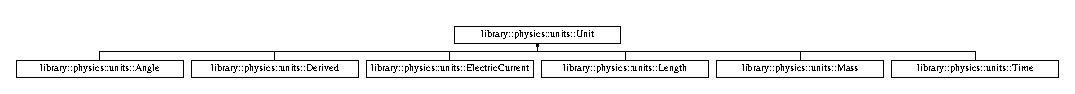
\includegraphics[height=0.811594cm]{classlibrary_1_1physics_1_1units_1_1_unit}
\end{center}
\end{figure}
\subsection*{Public Types}
\begin{DoxyCompactItemize}
\item 
enum \hyperlink{classlibrary_1_1physics_1_1units_1_1_unit_a828bc1b6ad6fa5cbef904ea0fede986a}{Type} \{ \newline
\hyperlink{classlibrary_1_1physics_1_1units_1_1_unit_a828bc1b6ad6fa5cbef904ea0fede986aaec0fc0100c4fc1ce4eea230c3dc10360}{Type\+::\+Undefined}, 
\hyperlink{classlibrary_1_1physics_1_1units_1_1_unit_a828bc1b6ad6fa5cbef904ea0fede986aaba2a9c6c8c77e03f83ef8bf543612275}{Type\+::\+Length}, 
\hyperlink{classlibrary_1_1physics_1_1units_1_1_unit_a828bc1b6ad6fa5cbef904ea0fede986aaff2864d6f652ee0ac254814f1ae4f4a8}{Type\+::\+Mass}, 
\hyperlink{classlibrary_1_1physics_1_1units_1_1_unit_a828bc1b6ad6fa5cbef904ea0fede986aaa76d4ef5f3f6a672bbfab2865563e530}{Type\+::\+Time}, 
\newline
\hyperlink{classlibrary_1_1physics_1_1units_1_1_unit_a828bc1b6ad6fa5cbef904ea0fede986aaee7a8e262285ed49ea1b4e4ae11525bd}{Type\+::\+Temperature}, 
\hyperlink{classlibrary_1_1physics_1_1units_1_1_unit_a828bc1b6ad6fa5cbef904ea0fede986aa9a60fd92ac6161bffa549ef2cd17f05e}{Type\+::\+Electric\+Current}, 
\hyperlink{classlibrary_1_1physics_1_1units_1_1_unit_a828bc1b6ad6fa5cbef904ea0fede986aae91a9eb4f5dcc51ea18e180ea981d6ae}{Type\+::\+Luminous\+Intensity}, 
\hyperlink{classlibrary_1_1physics_1_1units_1_1_unit_a828bc1b6ad6fa5cbef904ea0fede986aa0e77a10e9579997fa646fbda4118e108}{Type\+::\+Derived}
 \}
\end{DoxyCompactItemize}
\subsection*{Public Member Functions}
\begin{DoxyCompactItemize}
\item 
\hyperlink{classlibrary_1_1physics_1_1units_1_1_unit_a52369bb8717bfe8d04d7dcb992903208}{Unit} (const \hyperlink{classlibrary_1_1physics_1_1units_1_1_unit_a828bc1b6ad6fa5cbef904ea0fede986a}{Unit\+::\+Type} \&a\+Type, const Real \&a\+Value)
\item 
virtual \hyperlink{classlibrary_1_1physics_1_1units_1_1_unit_a6c50741e149602a9fecf3b45100463a0}{$\sim$\+Unit} ()=0
\item 
virtual \hyperlink{classlibrary_1_1physics_1_1units_1_1_unit}{Unit} $\ast$ \hyperlink{classlibrary_1_1physics_1_1units_1_1_unit_aff727141d73acddfae382e5e375f4640}{clone} () const =0
\item 
bool \hyperlink{classlibrary_1_1physics_1_1units_1_1_unit_ad7b6273fa1232ff0d26f98c2af39d183}{operator==} (const \hyperlink{classlibrary_1_1physics_1_1units_1_1_unit}{Unit} \&a\+Unit) const
\item 
bool \hyperlink{classlibrary_1_1physics_1_1units_1_1_unit_a68d7c6e97c9748b43b55b5f74e0f9cda}{operator!=} (const \hyperlink{classlibrary_1_1physics_1_1units_1_1_unit}{Unit} \&a\+Unit) const
\item 
virtual bool \hyperlink{classlibrary_1_1physics_1_1units_1_1_unit_a5ce011c1ffa0fce4cf1f5d42ff06ee78}{is\+Defined} () const
\item 
bool \hyperlink{classlibrary_1_1physics_1_1units_1_1_unit_a034d99479240b780ab15dbc9eec629f0}{is\+Zero} () const
\item 
const Real \& \hyperlink{classlibrary_1_1physics_1_1units_1_1_unit_a836f37ccb8db8220064f6718d3236f32}{access\+Value} () const
\item 
\hyperlink{classlibrary_1_1physics_1_1units_1_1_unit_a828bc1b6ad6fa5cbef904ea0fede986a}{Unit\+::\+Type} \hyperlink{classlibrary_1_1physics_1_1units_1_1_unit_a4f4e6ba62e833324970a06c29685488a}{get\+Type} () const
\item 
Real \hyperlink{classlibrary_1_1physics_1_1units_1_1_unit_ab6541add236a0c2e5bbfb4b5b35126fb}{get\+Value} () const
\item 
virtual String \hyperlink{classlibrary_1_1physics_1_1units_1_1_unit_ad7364d457300e36413323c4aebce8029}{to\+String} (const Integer \&a\+Precision=Integer\+::\+Undefined()) const =0
\item 
Real \& \hyperlink{classlibrary_1_1physics_1_1units_1_1_unit_a73cd28e6cae2cd36ab65bdeaf9814e8f}{access\+Value} ()
\item 
void \hyperlink{classlibrary_1_1physics_1_1units_1_1_unit_a0d61125a36ae706eb4800564fb7c5e54}{set\+Value} (const Real \&a\+Value)
\end{DoxyCompactItemize}


\subsection{Detailed Description}
\hyperlink{classlibrary_1_1physics_1_1units_1_1_unit}{Unit}. 

https\+://en.wikipedia.\+org/wiki/\+S\+I\+\_\+base\+\_\+unit

\begin{DoxyNote}{Note}
Could be (greatly) improved using templating... 

\href{https://benjaminjurke.com/content/articles/2015/compile-time-numerical-unit-dimension-checking/}{\tt https\+://benjaminjurke.\+com/content/articles/2015/compile-\/time-\/numerical-\/unit-\/dimension-\/checking/} 

\href{https://github.com/nholthaus/units}{\tt https\+://github.\+com/nholthaus/units} 

\href{https://www.boost.org/doc/libs/1_67_0/doc/html/boost_units.html}{\tt https\+://www.\+boost.\+org/doc/libs/1\+\_\+67\+\_\+0/doc/html/boost\+\_\+units.\+html} 
\end{DoxyNote}


\subsection{Member Enumeration Documentation}
\mbox{\Hypertarget{classlibrary_1_1physics_1_1units_1_1_unit_a828bc1b6ad6fa5cbef904ea0fede986a}\label{classlibrary_1_1physics_1_1units_1_1_unit_a828bc1b6ad6fa5cbef904ea0fede986a}} 
\index{library\+::physics\+::units\+::\+Unit@{library\+::physics\+::units\+::\+Unit}!Type@{Type}}
\index{Type@{Type}!library\+::physics\+::units\+::\+Unit@{library\+::physics\+::units\+::\+Unit}}
\subsubsection{\texorpdfstring{Type}{Type}}
{\footnotesize\ttfamily enum \hyperlink{classlibrary_1_1physics_1_1units_1_1_unit_a828bc1b6ad6fa5cbef904ea0fede986a}{library\+::physics\+::units\+::\+Unit\+::\+Type}\hspace{0.3cm}{\ttfamily [strong]}}

\begin{DoxyEnumFields}{Enumerator}
\raisebox{\heightof{T}}[0pt][0pt]{\index{Undefined@{Undefined}!library\+::physics\+::units\+::\+Unit@{library\+::physics\+::units\+::\+Unit}}\index{library\+::physics\+::units\+::\+Unit@{library\+::physics\+::units\+::\+Unit}!Undefined@{Undefined}}}\mbox{\Hypertarget{classlibrary_1_1physics_1_1units_1_1_unit_a828bc1b6ad6fa5cbef904ea0fede986aaec0fc0100c4fc1ce4eea230c3dc10360}\label{classlibrary_1_1physics_1_1units_1_1_unit_a828bc1b6ad6fa5cbef904ea0fede986aaec0fc0100c4fc1ce4eea230c3dc10360}} 
Undefined&\\
\hline

\raisebox{\heightof{T}}[0pt][0pt]{\index{Length@{Length}!library\+::physics\+::units\+::\+Unit@{library\+::physics\+::units\+::\+Unit}}\index{library\+::physics\+::units\+::\+Unit@{library\+::physics\+::units\+::\+Unit}!Length@{Length}}}\mbox{\Hypertarget{classlibrary_1_1physics_1_1units_1_1_unit_a828bc1b6ad6fa5cbef904ea0fede986aaba2a9c6c8c77e03f83ef8bf543612275}\label{classlibrary_1_1physics_1_1units_1_1_unit_a828bc1b6ad6fa5cbef904ea0fede986aaba2a9c6c8c77e03f83ef8bf543612275}} 
Length&\\
\hline

\raisebox{\heightof{T}}[0pt][0pt]{\index{Mass@{Mass}!library\+::physics\+::units\+::\+Unit@{library\+::physics\+::units\+::\+Unit}}\index{library\+::physics\+::units\+::\+Unit@{library\+::physics\+::units\+::\+Unit}!Mass@{Mass}}}\mbox{\Hypertarget{classlibrary_1_1physics_1_1units_1_1_unit_a828bc1b6ad6fa5cbef904ea0fede986aaff2864d6f652ee0ac254814f1ae4f4a8}\label{classlibrary_1_1physics_1_1units_1_1_unit_a828bc1b6ad6fa5cbef904ea0fede986aaff2864d6f652ee0ac254814f1ae4f4a8}} 
Mass&\\
\hline

\raisebox{\heightof{T}}[0pt][0pt]{\index{Time@{Time}!library\+::physics\+::units\+::\+Unit@{library\+::physics\+::units\+::\+Unit}}\index{library\+::physics\+::units\+::\+Unit@{library\+::physics\+::units\+::\+Unit}!Time@{Time}}}\mbox{\Hypertarget{classlibrary_1_1physics_1_1units_1_1_unit_a828bc1b6ad6fa5cbef904ea0fede986aaa76d4ef5f3f6a672bbfab2865563e530}\label{classlibrary_1_1physics_1_1units_1_1_unit_a828bc1b6ad6fa5cbef904ea0fede986aaa76d4ef5f3f6a672bbfab2865563e530}} 
Time&\\
\hline

\raisebox{\heightof{T}}[0pt][0pt]{\index{Temperature@{Temperature}!library\+::physics\+::units\+::\+Unit@{library\+::physics\+::units\+::\+Unit}}\index{library\+::physics\+::units\+::\+Unit@{library\+::physics\+::units\+::\+Unit}!Temperature@{Temperature}}}\mbox{\Hypertarget{classlibrary_1_1physics_1_1units_1_1_unit_a828bc1b6ad6fa5cbef904ea0fede986aaee7a8e262285ed49ea1b4e4ae11525bd}\label{classlibrary_1_1physics_1_1units_1_1_unit_a828bc1b6ad6fa5cbef904ea0fede986aaee7a8e262285ed49ea1b4e4ae11525bd}} 
Temperature&\\
\hline

\raisebox{\heightof{T}}[0pt][0pt]{\index{Electric\+Current@{Electric\+Current}!library\+::physics\+::units\+::\+Unit@{library\+::physics\+::units\+::\+Unit}}\index{library\+::physics\+::units\+::\+Unit@{library\+::physics\+::units\+::\+Unit}!Electric\+Current@{Electric\+Current}}}\mbox{\Hypertarget{classlibrary_1_1physics_1_1units_1_1_unit_a828bc1b6ad6fa5cbef904ea0fede986aa9a60fd92ac6161bffa549ef2cd17f05e}\label{classlibrary_1_1physics_1_1units_1_1_unit_a828bc1b6ad6fa5cbef904ea0fede986aa9a60fd92ac6161bffa549ef2cd17f05e}} 
Electric\+Current&\\
\hline

\raisebox{\heightof{T}}[0pt][0pt]{\index{Luminous\+Intensity@{Luminous\+Intensity}!library\+::physics\+::units\+::\+Unit@{library\+::physics\+::units\+::\+Unit}}\index{library\+::physics\+::units\+::\+Unit@{library\+::physics\+::units\+::\+Unit}!Luminous\+Intensity@{Luminous\+Intensity}}}\mbox{\Hypertarget{classlibrary_1_1physics_1_1units_1_1_unit_a828bc1b6ad6fa5cbef904ea0fede986aae91a9eb4f5dcc51ea18e180ea981d6ae}\label{classlibrary_1_1physics_1_1units_1_1_unit_a828bc1b6ad6fa5cbef904ea0fede986aae91a9eb4f5dcc51ea18e180ea981d6ae}} 
Luminous\+Intensity&\\
\hline

\raisebox{\heightof{T}}[0pt][0pt]{\index{Derived@{Derived}!library\+::physics\+::units\+::\+Unit@{library\+::physics\+::units\+::\+Unit}}\index{library\+::physics\+::units\+::\+Unit@{library\+::physics\+::units\+::\+Unit}!Derived@{Derived}}}\mbox{\Hypertarget{classlibrary_1_1physics_1_1units_1_1_unit_a828bc1b6ad6fa5cbef904ea0fede986aa0e77a10e9579997fa646fbda4118e108}\label{classlibrary_1_1physics_1_1units_1_1_unit_a828bc1b6ad6fa5cbef904ea0fede986aa0e77a10e9579997fa646fbda4118e108}} 
Derived&\\
\hline

\end{DoxyEnumFields}


\subsection{Constructor \& Destructor Documentation}
\mbox{\Hypertarget{classlibrary_1_1physics_1_1units_1_1_unit_a52369bb8717bfe8d04d7dcb992903208}\label{classlibrary_1_1physics_1_1units_1_1_unit_a52369bb8717bfe8d04d7dcb992903208}} 
\index{library\+::physics\+::units\+::\+Unit@{library\+::physics\+::units\+::\+Unit}!Unit@{Unit}}
\index{Unit@{Unit}!library\+::physics\+::units\+::\+Unit@{library\+::physics\+::units\+::\+Unit}}
\subsubsection{\texorpdfstring{Unit()}{Unit()}}
{\footnotesize\ttfamily library\+::physics\+::units\+::\+Unit\+::\+Unit (\begin{DoxyParamCaption}\item[{const \hyperlink{classlibrary_1_1physics_1_1units_1_1_unit_a828bc1b6ad6fa5cbef904ea0fede986a}{Unit\+::\+Type} \&}]{a\+Type,  }\item[{const Real \&}]{a\+Value }\end{DoxyParamCaption})}

\mbox{\Hypertarget{classlibrary_1_1physics_1_1units_1_1_unit_a6c50741e149602a9fecf3b45100463a0}\label{classlibrary_1_1physics_1_1units_1_1_unit_a6c50741e149602a9fecf3b45100463a0}} 
\index{library\+::physics\+::units\+::\+Unit@{library\+::physics\+::units\+::\+Unit}!````~Unit@{$\sim$\+Unit}}
\index{````~Unit@{$\sim$\+Unit}!library\+::physics\+::units\+::\+Unit@{library\+::physics\+::units\+::\+Unit}}
\subsubsection{\texorpdfstring{$\sim$\+Unit()}{~Unit()}}
{\footnotesize\ttfamily library\+::physics\+::units\+::\+Unit\+::$\sim$\+Unit (\begin{DoxyParamCaption}{ }\end{DoxyParamCaption})\hspace{0.3cm}{\ttfamily [pure virtual]}}



\subsection{Member Function Documentation}
\mbox{\Hypertarget{classlibrary_1_1physics_1_1units_1_1_unit_a836f37ccb8db8220064f6718d3236f32}\label{classlibrary_1_1physics_1_1units_1_1_unit_a836f37ccb8db8220064f6718d3236f32}} 
\index{library\+::physics\+::units\+::\+Unit@{library\+::physics\+::units\+::\+Unit}!access\+Value@{access\+Value}}
\index{access\+Value@{access\+Value}!library\+::physics\+::units\+::\+Unit@{library\+::physics\+::units\+::\+Unit}}
\subsubsection{\texorpdfstring{access\+Value()}{accessValue()}\hspace{0.1cm}{\footnotesize\ttfamily [1/2]}}
{\footnotesize\ttfamily const Real \& library\+::physics\+::units\+::\+Unit\+::access\+Value (\begin{DoxyParamCaption}{ }\end{DoxyParamCaption}) const}

\mbox{\Hypertarget{classlibrary_1_1physics_1_1units_1_1_unit_a73cd28e6cae2cd36ab65bdeaf9814e8f}\label{classlibrary_1_1physics_1_1units_1_1_unit_a73cd28e6cae2cd36ab65bdeaf9814e8f}} 
\index{library\+::physics\+::units\+::\+Unit@{library\+::physics\+::units\+::\+Unit}!access\+Value@{access\+Value}}
\index{access\+Value@{access\+Value}!library\+::physics\+::units\+::\+Unit@{library\+::physics\+::units\+::\+Unit}}
\subsubsection{\texorpdfstring{access\+Value()}{accessValue()}\hspace{0.1cm}{\footnotesize\ttfamily [2/2]}}
{\footnotesize\ttfamily Real \& library\+::physics\+::units\+::\+Unit\+::access\+Value (\begin{DoxyParamCaption}{ }\end{DoxyParamCaption})}

\mbox{\Hypertarget{classlibrary_1_1physics_1_1units_1_1_unit_aff727141d73acddfae382e5e375f4640}\label{classlibrary_1_1physics_1_1units_1_1_unit_aff727141d73acddfae382e5e375f4640}} 
\index{library\+::physics\+::units\+::\+Unit@{library\+::physics\+::units\+::\+Unit}!clone@{clone}}
\index{clone@{clone}!library\+::physics\+::units\+::\+Unit@{library\+::physics\+::units\+::\+Unit}}
\subsubsection{\texorpdfstring{clone()}{clone()}}
{\footnotesize\ttfamily virtual \hyperlink{classlibrary_1_1physics_1_1units_1_1_unit}{Unit}$\ast$ library\+::physics\+::units\+::\+Unit\+::clone (\begin{DoxyParamCaption}{ }\end{DoxyParamCaption}) const\hspace{0.3cm}{\ttfamily [pure virtual]}}



Implemented in \hyperlink{classlibrary_1_1physics_1_1units_1_1_derived_a6328e9f5bcf35f1c587c20f9c3fdb497}{library\+::physics\+::units\+::\+Derived}, \hyperlink{classlibrary_1_1physics_1_1units_1_1_angle_add51af263128e384d3d89827d0f70dcf}{library\+::physics\+::units\+::\+Angle}, \hyperlink{classlibrary_1_1physics_1_1units_1_1_time_a8745ebee6707751e91137c3e87782b59}{library\+::physics\+::units\+::\+Time}, \hyperlink{classlibrary_1_1physics_1_1units_1_1_length_ae06162cf9f3d140a3b53e156a4cb3309}{library\+::physics\+::units\+::\+Length}, \hyperlink{classlibrary_1_1physics_1_1units_1_1_mass_a7a09438b05edbe4b21a05ec234a6372f}{library\+::physics\+::units\+::\+Mass}, and \hyperlink{classlibrary_1_1physics_1_1units_1_1_electric_current_a3bde9c5bfa0834e43428a28c7059e32f}{library\+::physics\+::units\+::\+Electric\+Current}.

\mbox{\Hypertarget{classlibrary_1_1physics_1_1units_1_1_unit_a4f4e6ba62e833324970a06c29685488a}\label{classlibrary_1_1physics_1_1units_1_1_unit_a4f4e6ba62e833324970a06c29685488a}} 
\index{library\+::physics\+::units\+::\+Unit@{library\+::physics\+::units\+::\+Unit}!get\+Type@{get\+Type}}
\index{get\+Type@{get\+Type}!library\+::physics\+::units\+::\+Unit@{library\+::physics\+::units\+::\+Unit}}
\subsubsection{\texorpdfstring{get\+Type()}{getType()}}
{\footnotesize\ttfamily \hyperlink{classlibrary_1_1physics_1_1units_1_1_unit_a828bc1b6ad6fa5cbef904ea0fede986a}{Unit\+::\+Type} library\+::physics\+::units\+::\+Unit\+::get\+Type (\begin{DoxyParamCaption}{ }\end{DoxyParamCaption}) const}

\mbox{\Hypertarget{classlibrary_1_1physics_1_1units_1_1_unit_ab6541add236a0c2e5bbfb4b5b35126fb}\label{classlibrary_1_1physics_1_1units_1_1_unit_ab6541add236a0c2e5bbfb4b5b35126fb}} 
\index{library\+::physics\+::units\+::\+Unit@{library\+::physics\+::units\+::\+Unit}!get\+Value@{get\+Value}}
\index{get\+Value@{get\+Value}!library\+::physics\+::units\+::\+Unit@{library\+::physics\+::units\+::\+Unit}}
\subsubsection{\texorpdfstring{get\+Value()}{getValue()}}
{\footnotesize\ttfamily Real library\+::physics\+::units\+::\+Unit\+::get\+Value (\begin{DoxyParamCaption}{ }\end{DoxyParamCaption}) const}

\mbox{\Hypertarget{classlibrary_1_1physics_1_1units_1_1_unit_a5ce011c1ffa0fce4cf1f5d42ff06ee78}\label{classlibrary_1_1physics_1_1units_1_1_unit_a5ce011c1ffa0fce4cf1f5d42ff06ee78}} 
\index{library\+::physics\+::units\+::\+Unit@{library\+::physics\+::units\+::\+Unit}!is\+Defined@{is\+Defined}}
\index{is\+Defined@{is\+Defined}!library\+::physics\+::units\+::\+Unit@{library\+::physics\+::units\+::\+Unit}}
\subsubsection{\texorpdfstring{is\+Defined()}{isDefined()}}
{\footnotesize\ttfamily bool library\+::physics\+::units\+::\+Unit\+::is\+Defined (\begin{DoxyParamCaption}{ }\end{DoxyParamCaption}) const\hspace{0.3cm}{\ttfamily [virtual]}}



Reimplemented in \hyperlink{classlibrary_1_1physics_1_1units_1_1_derived_a26c20c57fc3a7c2fb2ff215d6d4687a2}{library\+::physics\+::units\+::\+Derived}, \hyperlink{classlibrary_1_1physics_1_1units_1_1_angle_a77c7849734ce02b55e070fb88fd87f71}{library\+::physics\+::units\+::\+Angle}, \hyperlink{classlibrary_1_1physics_1_1units_1_1_length_a0249a542e7cc613e6a39275b4e37bd05}{library\+::physics\+::units\+::\+Length}, \hyperlink{classlibrary_1_1physics_1_1units_1_1_time_ab62163386c3253277c5ba71782261cad}{library\+::physics\+::units\+::\+Time}, \hyperlink{classlibrary_1_1physics_1_1units_1_1_mass_a0efde6eb08d6b79baa84229746776b6a}{library\+::physics\+::units\+::\+Mass}, and \hyperlink{classlibrary_1_1physics_1_1units_1_1_electric_current_a52796b966074a631c569ac93d22869af}{library\+::physics\+::units\+::\+Electric\+Current}.

\mbox{\Hypertarget{classlibrary_1_1physics_1_1units_1_1_unit_a034d99479240b780ab15dbc9eec629f0}\label{classlibrary_1_1physics_1_1units_1_1_unit_a034d99479240b780ab15dbc9eec629f0}} 
\index{library\+::physics\+::units\+::\+Unit@{library\+::physics\+::units\+::\+Unit}!is\+Zero@{is\+Zero}}
\index{is\+Zero@{is\+Zero}!library\+::physics\+::units\+::\+Unit@{library\+::physics\+::units\+::\+Unit}}
\subsubsection{\texorpdfstring{is\+Zero()}{isZero()}}
{\footnotesize\ttfamily bool library\+::physics\+::units\+::\+Unit\+::is\+Zero (\begin{DoxyParamCaption}{ }\end{DoxyParamCaption}) const}

\mbox{\Hypertarget{classlibrary_1_1physics_1_1units_1_1_unit_a68d7c6e97c9748b43b55b5f74e0f9cda}\label{classlibrary_1_1physics_1_1units_1_1_unit_a68d7c6e97c9748b43b55b5f74e0f9cda}} 
\index{library\+::physics\+::units\+::\+Unit@{library\+::physics\+::units\+::\+Unit}!operator"!=@{operator"!=}}
\index{operator"!=@{operator"!=}!library\+::physics\+::units\+::\+Unit@{library\+::physics\+::units\+::\+Unit}}
\subsubsection{\texorpdfstring{operator"!=()}{operator!=()}}
{\footnotesize\ttfamily bool library\+::physics\+::units\+::\+Unit\+::operator!= (\begin{DoxyParamCaption}\item[{const \hyperlink{classlibrary_1_1physics_1_1units_1_1_unit}{Unit} \&}]{a\+Unit }\end{DoxyParamCaption}) const}

\mbox{\Hypertarget{classlibrary_1_1physics_1_1units_1_1_unit_ad7b6273fa1232ff0d26f98c2af39d183}\label{classlibrary_1_1physics_1_1units_1_1_unit_ad7b6273fa1232ff0d26f98c2af39d183}} 
\index{library\+::physics\+::units\+::\+Unit@{library\+::physics\+::units\+::\+Unit}!operator==@{operator==}}
\index{operator==@{operator==}!library\+::physics\+::units\+::\+Unit@{library\+::physics\+::units\+::\+Unit}}
\subsubsection{\texorpdfstring{operator==()}{operator==()}}
{\footnotesize\ttfamily bool library\+::physics\+::units\+::\+Unit\+::operator== (\begin{DoxyParamCaption}\item[{const \hyperlink{classlibrary_1_1physics_1_1units_1_1_unit}{Unit} \&}]{a\+Unit }\end{DoxyParamCaption}) const}

\mbox{\Hypertarget{classlibrary_1_1physics_1_1units_1_1_unit_a0d61125a36ae706eb4800564fb7c5e54}\label{classlibrary_1_1physics_1_1units_1_1_unit_a0d61125a36ae706eb4800564fb7c5e54}} 
\index{library\+::physics\+::units\+::\+Unit@{library\+::physics\+::units\+::\+Unit}!set\+Value@{set\+Value}}
\index{set\+Value@{set\+Value}!library\+::physics\+::units\+::\+Unit@{library\+::physics\+::units\+::\+Unit}}
\subsubsection{\texorpdfstring{set\+Value()}{setValue()}}
{\footnotesize\ttfamily void library\+::physics\+::units\+::\+Unit\+::set\+Value (\begin{DoxyParamCaption}\item[{const Real \&}]{a\+Value }\end{DoxyParamCaption})}

\mbox{\Hypertarget{classlibrary_1_1physics_1_1units_1_1_unit_ad7364d457300e36413323c4aebce8029}\label{classlibrary_1_1physics_1_1units_1_1_unit_ad7364d457300e36413323c4aebce8029}} 
\index{library\+::physics\+::units\+::\+Unit@{library\+::physics\+::units\+::\+Unit}!to\+String@{to\+String}}
\index{to\+String@{to\+String}!library\+::physics\+::units\+::\+Unit@{library\+::physics\+::units\+::\+Unit}}
\subsubsection{\texorpdfstring{to\+String()}{toString()}}
{\footnotesize\ttfamily virtual String library\+::physics\+::units\+::\+Unit\+::to\+String (\begin{DoxyParamCaption}\item[{const Integer \&}]{a\+Precision = {\ttfamily Integer\+:\+:Undefined()} }\end{DoxyParamCaption}) const\hspace{0.3cm}{\ttfamily [pure virtual]}}



Implemented in \hyperlink{classlibrary_1_1physics_1_1units_1_1_derived_a3626d6c77e6753f44232067856fde9d1}{library\+::physics\+::units\+::\+Derived}, \hyperlink{classlibrary_1_1physics_1_1units_1_1_angle_aae6b7bd4e028ea7719f5a712ca19a86c}{library\+::physics\+::units\+::\+Angle}, \hyperlink{classlibrary_1_1physics_1_1units_1_1_length_aea1d96e6930f7e6e6383e78c55219a64}{library\+::physics\+::units\+::\+Length}, \hyperlink{classlibrary_1_1physics_1_1units_1_1_time_a6f56977493a45d334bb53bc4246888c4}{library\+::physics\+::units\+::\+Time}, \hyperlink{classlibrary_1_1physics_1_1units_1_1_mass_a6e7757920752ac9f6918525d6fadb31e}{library\+::physics\+::units\+::\+Mass}, and \hyperlink{classlibrary_1_1physics_1_1units_1_1_electric_current_ab2325214012e6f50350a0dec575d877f}{library\+::physics\+::units\+::\+Electric\+Current}.



The documentation for this class was generated from the following files\+:\begin{DoxyCompactItemize}
\item 
include/\+Library/\+Physics/\+Units/\hyperlink{_units_2_unit_8hpp}{Unit.\+hpp}\item 
src/\+Library/\+Physics/\+Units/\hyperlink{_units_2_unit_8cpp}{Unit.\+cpp}\end{DoxyCompactItemize}

\hypertarget{classlibrary_1_1physics_1_1coord_1_1_velocity}{}\section{library\+:\+:physics\+:\+:coord\+:\+:Velocity Class Reference}
\label{classlibrary_1_1physics_1_1coord_1_1_velocity}\index{library\+::physics\+::coord\+::\+Velocity@{library\+::physics\+::coord\+::\+Velocity}}


\hyperlink{classlibrary_1_1physics_1_1coord_1_1_velocity}{Velocity}.  




{\ttfamily \#include $<$Velocity.\+hpp$>$}

\subsection*{Public Types}
\begin{DoxyCompactItemize}
\item 
enum \hyperlink{classlibrary_1_1physics_1_1coord_1_1_velocity_a8bbc811932c454dbe0ab8b56f1b2c0b3}{Unit} \{ \hyperlink{classlibrary_1_1physics_1_1coord_1_1_velocity_a8bbc811932c454dbe0ab8b56f1b2c0b3aec0fc0100c4fc1ce4eea230c3dc10360}{Unit\+::\+Undefined}, 
\hyperlink{classlibrary_1_1physics_1_1coord_1_1_velocity_a8bbc811932c454dbe0ab8b56f1b2c0b3a0af408165b5f88fcd7b687312b754ade}{Unit\+::\+Meter\+Per\+Second}
 \}
\end{DoxyCompactItemize}
\subsection*{Public Member Functions}
\begin{DoxyCompactItemize}
\item 
\hyperlink{classlibrary_1_1physics_1_1coord_1_1_velocity_a4e2058adb91710a45a6d8165fae9e8e0}{Velocity} (const Vector3d \&a\+Coordinate\+Set, const \hyperlink{classlibrary_1_1physics_1_1coord_1_1_velocity_a8bbc811932c454dbe0ab8b56f1b2c0b3}{Velocity\+::\+Unit} \&a\+Unit, const Shared$<$ const \hyperlink{classlibrary_1_1physics_1_1coord_1_1_frame}{Frame} $>$ \&a\+Frame)
\item 
bool \hyperlink{classlibrary_1_1physics_1_1coord_1_1_velocity_afa328f637276f940812aea194836aeb9}{operator==} (const \hyperlink{classlibrary_1_1physics_1_1coord_1_1_velocity}{Velocity} \&a\+Velocity) const
\item 
bool \hyperlink{classlibrary_1_1physics_1_1coord_1_1_velocity_aaa76cc11a5ecbbff21839f1ea5f8aa8e}{operator!=} (const \hyperlink{classlibrary_1_1physics_1_1coord_1_1_velocity}{Velocity} \&a\+Velocity) const
\item 
bool \hyperlink{classlibrary_1_1physics_1_1coord_1_1_velocity_a5487f6d50e13d2262bf0726ed8536c99}{is\+Defined} () const
\item 
const Vector3d \& \hyperlink{classlibrary_1_1physics_1_1coord_1_1_velocity_aea8fe9c62293e20393d9a662f277b0e7}{access\+Coordinates} () const
\item 
Shared$<$ const \hyperlink{classlibrary_1_1physics_1_1coord_1_1_frame}{Frame} $>$ \hyperlink{classlibrary_1_1physics_1_1coord_1_1_velocity_a1d3dc032dba7937276b06649cb16a871}{access\+Frame} () const
\item 
Vector3d \hyperlink{classlibrary_1_1physics_1_1coord_1_1_velocity_a1ac18f97a304ac026c2544292b89e030}{get\+Coordinates} () const
\item 
\hyperlink{classlibrary_1_1physics_1_1coord_1_1_velocity_a8bbc811932c454dbe0ab8b56f1b2c0b3}{Velocity\+::\+Unit} \hyperlink{classlibrary_1_1physics_1_1coord_1_1_velocity_aa04a5b82a46d5ea4e92bf53046a18494}{get\+Unit} () const
\item 
\hyperlink{classlibrary_1_1physics_1_1coord_1_1_velocity}{Velocity} \hyperlink{classlibrary_1_1physics_1_1coord_1_1_velocity_a814e6740d6b54cf5421d9aa7fc0f5958}{in\+Unit} (const \hyperlink{classlibrary_1_1physics_1_1coord_1_1_velocity_a8bbc811932c454dbe0ab8b56f1b2c0b3}{Velocity\+::\+Unit} \&a\+Unit) const
\item 
\hyperlink{classlibrary_1_1physics_1_1coord_1_1_velocity}{Velocity} \hyperlink{classlibrary_1_1physics_1_1coord_1_1_velocity_ac2e825fe682f526884764218425a14b7}{in\+Frame} (const \hyperlink{classlibrary_1_1physics_1_1coord_1_1_position}{Position} \&a\+Position, const Shared$<$ const \hyperlink{classlibrary_1_1physics_1_1coord_1_1_frame}{Frame} $>$ \&a\+Frame, const \hyperlink{classlibrary_1_1physics_1_1time_1_1_instant}{Instant} \&an\+Instant) const
\item 
String \hyperlink{classlibrary_1_1physics_1_1coord_1_1_velocity_a16c176cadc68b384eb3d8e5594b316bd}{to\+String} (const Integer \&a\+Precision=Integer\+::\+Undefined()) const
\end{DoxyCompactItemize}
\subsection*{Static Public Member Functions}
\begin{DoxyCompactItemize}
\item 
static \hyperlink{classlibrary_1_1physics_1_1coord_1_1_velocity}{Velocity} \hyperlink{classlibrary_1_1physics_1_1coord_1_1_velocity_ae6480807520330e282b712805aa4fea5}{Undefined} ()
\item 
static \hyperlink{classlibrary_1_1physics_1_1coord_1_1_velocity}{Velocity} \hyperlink{classlibrary_1_1physics_1_1coord_1_1_velocity_ae00ee3d929b00160789cf33dcb448ae3}{Meters\+Per\+Second} (const Vector3d \&a\+Coordinate\+Set, const Shared$<$ const \hyperlink{classlibrary_1_1physics_1_1coord_1_1_frame}{Frame} $>$ \&a\+Frame)
\item 
static String \hyperlink{classlibrary_1_1physics_1_1coord_1_1_velocity_ad9a3d2d5759384f513f7790534e620a3}{String\+From\+Unit} (const \hyperlink{classlibrary_1_1physics_1_1coord_1_1_velocity_a8bbc811932c454dbe0ab8b56f1b2c0b3}{Velocity\+::\+Unit} \&a\+Unit)
\end{DoxyCompactItemize}
\subsection*{Friends}
\begin{DoxyCompactItemize}
\item 
std\+::ostream \& \hyperlink{classlibrary_1_1physics_1_1coord_1_1_velocity_ab3987a176df736aa7fa50aa763ed068b}{operator$<$$<$} (std\+::ostream \&an\+Output\+Stream, const \hyperlink{classlibrary_1_1physics_1_1coord_1_1_velocity}{Velocity} \&a\+Velocity)
\end{DoxyCompactItemize}


\subsection{Detailed Description}
\hyperlink{classlibrary_1_1physics_1_1coord_1_1_velocity}{Velocity}. 

\subsection{Member Enumeration Documentation}
\mbox{\Hypertarget{classlibrary_1_1physics_1_1coord_1_1_velocity_a8bbc811932c454dbe0ab8b56f1b2c0b3}\label{classlibrary_1_1physics_1_1coord_1_1_velocity_a8bbc811932c454dbe0ab8b56f1b2c0b3}} 
\index{library\+::physics\+::coord\+::\+Velocity@{library\+::physics\+::coord\+::\+Velocity}!Unit@{Unit}}
\index{Unit@{Unit}!library\+::physics\+::coord\+::\+Velocity@{library\+::physics\+::coord\+::\+Velocity}}
\subsubsection{\texorpdfstring{Unit}{Unit}}
{\footnotesize\ttfamily enum \hyperlink{classlibrary_1_1physics_1_1coord_1_1_velocity_a8bbc811932c454dbe0ab8b56f1b2c0b3}{library\+::physics\+::coord\+::\+Velocity\+::\+Unit}\hspace{0.3cm}{\ttfamily [strong]}}

\begin{DoxyEnumFields}{Enumerator}
\raisebox{\heightof{T}}[0pt][0pt]{\index{Undefined@{Undefined}!library\+::physics\+::coord\+::\+Velocity@{library\+::physics\+::coord\+::\+Velocity}}\index{library\+::physics\+::coord\+::\+Velocity@{library\+::physics\+::coord\+::\+Velocity}!Undefined@{Undefined}}}\mbox{\Hypertarget{classlibrary_1_1physics_1_1coord_1_1_velocity_a8bbc811932c454dbe0ab8b56f1b2c0b3aec0fc0100c4fc1ce4eea230c3dc10360}\label{classlibrary_1_1physics_1_1coord_1_1_velocity_a8bbc811932c454dbe0ab8b56f1b2c0b3aec0fc0100c4fc1ce4eea230c3dc10360}} 
Undefined&\\
\hline

\raisebox{\heightof{T}}[0pt][0pt]{\index{Meter\+Per\+Second@{Meter\+Per\+Second}!library\+::physics\+::coord\+::\+Velocity@{library\+::physics\+::coord\+::\+Velocity}}\index{library\+::physics\+::coord\+::\+Velocity@{library\+::physics\+::coord\+::\+Velocity}!Meter\+Per\+Second@{Meter\+Per\+Second}}}\mbox{\Hypertarget{classlibrary_1_1physics_1_1coord_1_1_velocity_a8bbc811932c454dbe0ab8b56f1b2c0b3a0af408165b5f88fcd7b687312b754ade}\label{classlibrary_1_1physics_1_1coord_1_1_velocity_a8bbc811932c454dbe0ab8b56f1b2c0b3a0af408165b5f88fcd7b687312b754ade}} 
Meter\+Per\+Second&\\
\hline

\end{DoxyEnumFields}


\subsection{Constructor \& Destructor Documentation}
\mbox{\Hypertarget{classlibrary_1_1physics_1_1coord_1_1_velocity_a4e2058adb91710a45a6d8165fae9e8e0}\label{classlibrary_1_1physics_1_1coord_1_1_velocity_a4e2058adb91710a45a6d8165fae9e8e0}} 
\index{library\+::physics\+::coord\+::\+Velocity@{library\+::physics\+::coord\+::\+Velocity}!Velocity@{Velocity}}
\index{Velocity@{Velocity}!library\+::physics\+::coord\+::\+Velocity@{library\+::physics\+::coord\+::\+Velocity}}
\subsubsection{\texorpdfstring{Velocity()}{Velocity()}}
{\footnotesize\ttfamily library\+::physics\+::coord\+::\+Velocity\+::\+Velocity (\begin{DoxyParamCaption}\item[{const Vector3d \&}]{a\+Coordinate\+Set,  }\item[{const \hyperlink{classlibrary_1_1physics_1_1coord_1_1_velocity_a8bbc811932c454dbe0ab8b56f1b2c0b3}{Velocity\+::\+Unit} \&}]{a\+Unit,  }\item[{const Shared$<$ const \hyperlink{classlibrary_1_1physics_1_1coord_1_1_frame}{Frame} $>$ \&}]{a\+Frame }\end{DoxyParamCaption})}



\subsection{Member Function Documentation}
\mbox{\Hypertarget{classlibrary_1_1physics_1_1coord_1_1_velocity_aea8fe9c62293e20393d9a662f277b0e7}\label{classlibrary_1_1physics_1_1coord_1_1_velocity_aea8fe9c62293e20393d9a662f277b0e7}} 
\index{library\+::physics\+::coord\+::\+Velocity@{library\+::physics\+::coord\+::\+Velocity}!access\+Coordinates@{access\+Coordinates}}
\index{access\+Coordinates@{access\+Coordinates}!library\+::physics\+::coord\+::\+Velocity@{library\+::physics\+::coord\+::\+Velocity}}
\subsubsection{\texorpdfstring{access\+Coordinates()}{accessCoordinates()}}
{\footnotesize\ttfamily const Vector3d \& library\+::physics\+::coord\+::\+Velocity\+::access\+Coordinates (\begin{DoxyParamCaption}{ }\end{DoxyParamCaption}) const}

\mbox{\Hypertarget{classlibrary_1_1physics_1_1coord_1_1_velocity_a1d3dc032dba7937276b06649cb16a871}\label{classlibrary_1_1physics_1_1coord_1_1_velocity_a1d3dc032dba7937276b06649cb16a871}} 
\index{library\+::physics\+::coord\+::\+Velocity@{library\+::physics\+::coord\+::\+Velocity}!access\+Frame@{access\+Frame}}
\index{access\+Frame@{access\+Frame}!library\+::physics\+::coord\+::\+Velocity@{library\+::physics\+::coord\+::\+Velocity}}
\subsubsection{\texorpdfstring{access\+Frame()}{accessFrame()}}
{\footnotesize\ttfamily Shared$<$ const \hyperlink{classlibrary_1_1physics_1_1coord_1_1_frame}{Frame} $>$ library\+::physics\+::coord\+::\+Velocity\+::access\+Frame (\begin{DoxyParamCaption}{ }\end{DoxyParamCaption}) const}

\mbox{\Hypertarget{classlibrary_1_1physics_1_1coord_1_1_velocity_a1ac18f97a304ac026c2544292b89e030}\label{classlibrary_1_1physics_1_1coord_1_1_velocity_a1ac18f97a304ac026c2544292b89e030}} 
\index{library\+::physics\+::coord\+::\+Velocity@{library\+::physics\+::coord\+::\+Velocity}!get\+Coordinates@{get\+Coordinates}}
\index{get\+Coordinates@{get\+Coordinates}!library\+::physics\+::coord\+::\+Velocity@{library\+::physics\+::coord\+::\+Velocity}}
\subsubsection{\texorpdfstring{get\+Coordinates()}{getCoordinates()}}
{\footnotesize\ttfamily Vector3d library\+::physics\+::coord\+::\+Velocity\+::get\+Coordinates (\begin{DoxyParamCaption}{ }\end{DoxyParamCaption}) const}

\mbox{\Hypertarget{classlibrary_1_1physics_1_1coord_1_1_velocity_aa04a5b82a46d5ea4e92bf53046a18494}\label{classlibrary_1_1physics_1_1coord_1_1_velocity_aa04a5b82a46d5ea4e92bf53046a18494}} 
\index{library\+::physics\+::coord\+::\+Velocity@{library\+::physics\+::coord\+::\+Velocity}!get\+Unit@{get\+Unit}}
\index{get\+Unit@{get\+Unit}!library\+::physics\+::coord\+::\+Velocity@{library\+::physics\+::coord\+::\+Velocity}}
\subsubsection{\texorpdfstring{get\+Unit()}{getUnit()}}
{\footnotesize\ttfamily \hyperlink{classlibrary_1_1physics_1_1coord_1_1_velocity_a8bbc811932c454dbe0ab8b56f1b2c0b3}{Velocity\+::\+Unit} library\+::physics\+::coord\+::\+Velocity\+::get\+Unit (\begin{DoxyParamCaption}{ }\end{DoxyParamCaption}) const}

\mbox{\Hypertarget{classlibrary_1_1physics_1_1coord_1_1_velocity_ac2e825fe682f526884764218425a14b7}\label{classlibrary_1_1physics_1_1coord_1_1_velocity_ac2e825fe682f526884764218425a14b7}} 
\index{library\+::physics\+::coord\+::\+Velocity@{library\+::physics\+::coord\+::\+Velocity}!in\+Frame@{in\+Frame}}
\index{in\+Frame@{in\+Frame}!library\+::physics\+::coord\+::\+Velocity@{library\+::physics\+::coord\+::\+Velocity}}
\subsubsection{\texorpdfstring{in\+Frame()}{inFrame()}}
{\footnotesize\ttfamily \hyperlink{classlibrary_1_1physics_1_1coord_1_1_velocity}{Velocity} library\+::physics\+::coord\+::\+Velocity\+::in\+Frame (\begin{DoxyParamCaption}\item[{const \hyperlink{classlibrary_1_1physics_1_1coord_1_1_position}{Position} \&}]{a\+Position,  }\item[{const Shared$<$ const \hyperlink{classlibrary_1_1physics_1_1coord_1_1_frame}{Frame} $>$ \&}]{a\+Frame,  }\item[{const \hyperlink{classlibrary_1_1physics_1_1time_1_1_instant}{Instant} \&}]{an\+Instant }\end{DoxyParamCaption}) const}

\mbox{\Hypertarget{classlibrary_1_1physics_1_1coord_1_1_velocity_a814e6740d6b54cf5421d9aa7fc0f5958}\label{classlibrary_1_1physics_1_1coord_1_1_velocity_a814e6740d6b54cf5421d9aa7fc0f5958}} 
\index{library\+::physics\+::coord\+::\+Velocity@{library\+::physics\+::coord\+::\+Velocity}!in\+Unit@{in\+Unit}}
\index{in\+Unit@{in\+Unit}!library\+::physics\+::coord\+::\+Velocity@{library\+::physics\+::coord\+::\+Velocity}}
\subsubsection{\texorpdfstring{in\+Unit()}{inUnit()}}
{\footnotesize\ttfamily \hyperlink{classlibrary_1_1physics_1_1coord_1_1_velocity}{Velocity} library\+::physics\+::coord\+::\+Velocity\+::in\+Unit (\begin{DoxyParamCaption}\item[{const \hyperlink{classlibrary_1_1physics_1_1coord_1_1_velocity_a8bbc811932c454dbe0ab8b56f1b2c0b3}{Velocity\+::\+Unit} \&}]{a\+Unit }\end{DoxyParamCaption}) const}

\mbox{\Hypertarget{classlibrary_1_1physics_1_1coord_1_1_velocity_a5487f6d50e13d2262bf0726ed8536c99}\label{classlibrary_1_1physics_1_1coord_1_1_velocity_a5487f6d50e13d2262bf0726ed8536c99}} 
\index{library\+::physics\+::coord\+::\+Velocity@{library\+::physics\+::coord\+::\+Velocity}!is\+Defined@{is\+Defined}}
\index{is\+Defined@{is\+Defined}!library\+::physics\+::coord\+::\+Velocity@{library\+::physics\+::coord\+::\+Velocity}}
\subsubsection{\texorpdfstring{is\+Defined()}{isDefined()}}
{\footnotesize\ttfamily bool library\+::physics\+::coord\+::\+Velocity\+::is\+Defined (\begin{DoxyParamCaption}{ }\end{DoxyParamCaption}) const}

\mbox{\Hypertarget{classlibrary_1_1physics_1_1coord_1_1_velocity_ae00ee3d929b00160789cf33dcb448ae3}\label{classlibrary_1_1physics_1_1coord_1_1_velocity_ae00ee3d929b00160789cf33dcb448ae3}} 
\index{library\+::physics\+::coord\+::\+Velocity@{library\+::physics\+::coord\+::\+Velocity}!Meters\+Per\+Second@{Meters\+Per\+Second}}
\index{Meters\+Per\+Second@{Meters\+Per\+Second}!library\+::physics\+::coord\+::\+Velocity@{library\+::physics\+::coord\+::\+Velocity}}
\subsubsection{\texorpdfstring{Meters\+Per\+Second()}{MetersPerSecond()}}
{\footnotesize\ttfamily \hyperlink{classlibrary_1_1physics_1_1coord_1_1_velocity}{Velocity} library\+::physics\+::coord\+::\+Velocity\+::\+Meters\+Per\+Second (\begin{DoxyParamCaption}\item[{const Vector3d \&}]{a\+Coordinate\+Set,  }\item[{const Shared$<$ const \hyperlink{classlibrary_1_1physics_1_1coord_1_1_frame}{Frame} $>$ \&}]{a\+Frame }\end{DoxyParamCaption})\hspace{0.3cm}{\ttfamily [static]}}

\mbox{\Hypertarget{classlibrary_1_1physics_1_1coord_1_1_velocity_aaa76cc11a5ecbbff21839f1ea5f8aa8e}\label{classlibrary_1_1physics_1_1coord_1_1_velocity_aaa76cc11a5ecbbff21839f1ea5f8aa8e}} 
\index{library\+::physics\+::coord\+::\+Velocity@{library\+::physics\+::coord\+::\+Velocity}!operator"!=@{operator"!=}}
\index{operator"!=@{operator"!=}!library\+::physics\+::coord\+::\+Velocity@{library\+::physics\+::coord\+::\+Velocity}}
\subsubsection{\texorpdfstring{operator"!=()}{operator!=()}}
{\footnotesize\ttfamily bool library\+::physics\+::coord\+::\+Velocity\+::operator!= (\begin{DoxyParamCaption}\item[{const \hyperlink{classlibrary_1_1physics_1_1coord_1_1_velocity}{Velocity} \&}]{a\+Velocity }\end{DoxyParamCaption}) const}

\mbox{\Hypertarget{classlibrary_1_1physics_1_1coord_1_1_velocity_afa328f637276f940812aea194836aeb9}\label{classlibrary_1_1physics_1_1coord_1_1_velocity_afa328f637276f940812aea194836aeb9}} 
\index{library\+::physics\+::coord\+::\+Velocity@{library\+::physics\+::coord\+::\+Velocity}!operator==@{operator==}}
\index{operator==@{operator==}!library\+::physics\+::coord\+::\+Velocity@{library\+::physics\+::coord\+::\+Velocity}}
\subsubsection{\texorpdfstring{operator==()}{operator==()}}
{\footnotesize\ttfamily bool library\+::physics\+::coord\+::\+Velocity\+::operator== (\begin{DoxyParamCaption}\item[{const \hyperlink{classlibrary_1_1physics_1_1coord_1_1_velocity}{Velocity} \&}]{a\+Velocity }\end{DoxyParamCaption}) const}

\mbox{\Hypertarget{classlibrary_1_1physics_1_1coord_1_1_velocity_ad9a3d2d5759384f513f7790534e620a3}\label{classlibrary_1_1physics_1_1coord_1_1_velocity_ad9a3d2d5759384f513f7790534e620a3}} 
\index{library\+::physics\+::coord\+::\+Velocity@{library\+::physics\+::coord\+::\+Velocity}!String\+From\+Unit@{String\+From\+Unit}}
\index{String\+From\+Unit@{String\+From\+Unit}!library\+::physics\+::coord\+::\+Velocity@{library\+::physics\+::coord\+::\+Velocity}}
\subsubsection{\texorpdfstring{String\+From\+Unit()}{StringFromUnit()}}
{\footnotesize\ttfamily String library\+::physics\+::coord\+::\+Velocity\+::\+String\+From\+Unit (\begin{DoxyParamCaption}\item[{const \hyperlink{classlibrary_1_1physics_1_1coord_1_1_velocity_a8bbc811932c454dbe0ab8b56f1b2c0b3}{Velocity\+::\+Unit} \&}]{a\+Unit }\end{DoxyParamCaption})\hspace{0.3cm}{\ttfamily [static]}}

\mbox{\Hypertarget{classlibrary_1_1physics_1_1coord_1_1_velocity_a16c176cadc68b384eb3d8e5594b316bd}\label{classlibrary_1_1physics_1_1coord_1_1_velocity_a16c176cadc68b384eb3d8e5594b316bd}} 
\index{library\+::physics\+::coord\+::\+Velocity@{library\+::physics\+::coord\+::\+Velocity}!to\+String@{to\+String}}
\index{to\+String@{to\+String}!library\+::physics\+::coord\+::\+Velocity@{library\+::physics\+::coord\+::\+Velocity}}
\subsubsection{\texorpdfstring{to\+String()}{toString()}}
{\footnotesize\ttfamily String library\+::physics\+::coord\+::\+Velocity\+::to\+String (\begin{DoxyParamCaption}\item[{const Integer \&}]{a\+Precision = {\ttfamily Integer\+:\+:Undefined()} }\end{DoxyParamCaption}) const}

\mbox{\Hypertarget{classlibrary_1_1physics_1_1coord_1_1_velocity_ae6480807520330e282b712805aa4fea5}\label{classlibrary_1_1physics_1_1coord_1_1_velocity_ae6480807520330e282b712805aa4fea5}} 
\index{library\+::physics\+::coord\+::\+Velocity@{library\+::physics\+::coord\+::\+Velocity}!Undefined@{Undefined}}
\index{Undefined@{Undefined}!library\+::physics\+::coord\+::\+Velocity@{library\+::physics\+::coord\+::\+Velocity}}
\subsubsection{\texorpdfstring{Undefined()}{Undefined()}}
{\footnotesize\ttfamily \hyperlink{classlibrary_1_1physics_1_1coord_1_1_velocity}{Velocity} library\+::physics\+::coord\+::\+Velocity\+::\+Undefined (\begin{DoxyParamCaption}{ }\end{DoxyParamCaption})\hspace{0.3cm}{\ttfamily [static]}}



\subsection{Friends And Related Function Documentation}
\mbox{\Hypertarget{classlibrary_1_1physics_1_1coord_1_1_velocity_ab3987a176df736aa7fa50aa763ed068b}\label{classlibrary_1_1physics_1_1coord_1_1_velocity_ab3987a176df736aa7fa50aa763ed068b}} 
\index{library\+::physics\+::coord\+::\+Velocity@{library\+::physics\+::coord\+::\+Velocity}!operator$<$$<$@{operator$<$$<$}}
\index{operator$<$$<$@{operator$<$$<$}!library\+::physics\+::coord\+::\+Velocity@{library\+::physics\+::coord\+::\+Velocity}}
\subsubsection{\texorpdfstring{operator$<$$<$}{operator<<}}
{\footnotesize\ttfamily std\+::ostream\& operator$<$$<$ (\begin{DoxyParamCaption}\item[{std\+::ostream \&}]{an\+Output\+Stream,  }\item[{const \hyperlink{classlibrary_1_1physics_1_1coord_1_1_velocity}{Velocity} \&}]{a\+Velocity }\end{DoxyParamCaption})\hspace{0.3cm}{\ttfamily [friend]}}



The documentation for this class was generated from the following files\+:\begin{DoxyCompactItemize}
\item 
include/\+Library/\+Physics/\+Coordinate/\hyperlink{_velocity_8hpp}{Velocity.\+hpp}\item 
src/\+Library/\+Physics/\+Coordinate/\hyperlink{_velocity_8cpp}{Velocity.\+cpp}\end{DoxyCompactItemize}

\chapter{File Documentation}
\hypertarget{_c_o_n_t_r_i_b_u_t_i_n_g_8md}{}\section{C\+O\+N\+T\+R\+I\+B\+U\+T\+I\+N\+G.\+md File Reference}
\label{_c_o_n_t_r_i_b_u_t_i_n_g_8md}\index{C\+O\+N\+T\+R\+I\+B\+U\+T\+I\+N\+G.\+md@{C\+O\+N\+T\+R\+I\+B\+U\+T\+I\+N\+G.\+md}}

\hypertarget{_tutorial_8md}{}\section{docs/\+Tutorial.md File Reference}
\label{_tutorial_8md}\index{docs/\+Tutorial.\+md@{docs/\+Tutorial.\+md}}

\hypertarget{_axes_8hpp}{}\section{include/\+Library/\+Physics/\+Coordinate/\+Axes.hpp File Reference}
\label{_axes_8hpp}\index{include/\+Library/\+Physics/\+Coordinate/\+Axes.\+hpp@{include/\+Library/\+Physics/\+Coordinate/\+Axes.\+hpp}}
{\ttfamily \#include $<$Library/\+Physics/\+Time/\+Instant.\+hpp$>$}\newline
{\ttfamily \#include $<$Library/\+Mathematics/\+Objects/\+Vector.\+hpp$>$}\newline
{\ttfamily \#include $<$Library/\+Core/\+Types/\+Shared.\+hpp$>$}\newline
\subsection*{Classes}
\begin{DoxyCompactItemize}
\item 
class \hyperlink{classlibrary_1_1physics_1_1coord_1_1_axes}{library\+::physics\+::coord\+::\+Axes}
\begin{DoxyCompactList}\small\item\em \hyperlink{classlibrary_1_1physics_1_1coord_1_1_axes}{Axes}. \end{DoxyCompactList}\end{DoxyCompactItemize}
\subsection*{Namespaces}
\begin{DoxyCompactItemize}
\item 
 \hyperlink{namespacelibrary}{library}
\item 
 \hyperlink{namespacelibrary_1_1physics}{library\+::physics}
\item 
 \hyperlink{namespacelibrary_1_1physics_1_1coord}{library\+::physics\+::coord}
\end{DoxyCompactItemize}


\subsection{Detailed Description}
Library ▸ Physics

\begin{DoxyAuthor}{Author}
Lucas Brémond \href{mailto:lucas@loftorbital.com}{\tt lucas@loftorbital.\+com}  Apache License 2.\+0 
\end{DoxyAuthor}

\hypertarget{_frame_8hpp}{}\section{include/\+Library/\+Physics/\+Coordinate/\+Frame.hpp File Reference}
\label{_frame_8hpp}\index{include/\+Library/\+Physics/\+Coordinate/\+Frame.\+hpp@{include/\+Library/\+Physics/\+Coordinate/\+Frame.\+hpp}}
{\ttfamily \#include $<$Library/\+Physics/\+Coordinate/\+Frame/\+Provider.\+hpp$>$}\newline
{\ttfamily \#include $<$Library/\+Physics/\+Coordinate/\+Transform.\+hpp$>$}\newline
{\ttfamily \#include $<$Library/\+Physics/\+Coordinate/\+Axes.\+hpp$>$}\newline
{\ttfamily \#include $<$Library/\+Physics/\+Coordinate/\+Velocity.\+hpp$>$}\newline
{\ttfamily \#include $<$Library/\+Physics/\+Coordinate/\+Position.\+hpp$>$}\newline
{\ttfamily \#include $<$Library/\+Mathematics/\+Objects/\+Vector.\+hpp$>$}\newline
{\ttfamily \#include $<$Library/\+Core/\+Types/\+String.\+hpp$>$}\newline
{\ttfamily \#include $<$Library/\+Core/\+Types/\+Real.\+hpp$>$}\newline
{\ttfamily \#include $<$Library/\+Core/\+Types/\+Integer.\+hpp$>$}\newline
{\ttfamily \#include $<$Library/\+Core/\+Types/\+Shared.\+hpp$>$}\newline
{\ttfamily \#include $<$memory$>$}\newline
\subsection*{Classes}
\begin{DoxyCompactItemize}
\item 
class \hyperlink{classlibrary_1_1physics_1_1coord_1_1_frame}{library\+::physics\+::coord\+::\+Frame}
\begin{DoxyCompactList}\small\item\em Reference frame. \end{DoxyCompactList}\end{DoxyCompactItemize}
\subsection*{Namespaces}
\begin{DoxyCompactItemize}
\item 
 \hyperlink{namespacelibrary}{library}
\item 
 \hyperlink{namespacelibrary_1_1physics}{library\+::physics}
\item 
 \hyperlink{namespacelibrary_1_1physics_1_1coord}{library\+::physics\+::coord}
\end{DoxyCompactItemize}


\subsection{Detailed Description}
Library ▸ Physics

\begin{DoxyAuthor}{Author}
Lucas Brémond \href{mailto:lucas@loftorbital.com}{\tt lucas@loftorbital.\+com}  Apache License 2.\+0 
\end{DoxyAuthor}

\hypertarget{_manager_8hpp}{}\section{include/\+Library/\+Physics/\+Coordinate/\+Frame/\+Manager.hpp File Reference}
\label{_manager_8hpp}\index{include/\+Library/\+Physics/\+Coordinate/\+Frame/\+Manager.\+hpp@{include/\+Library/\+Physics/\+Coordinate/\+Frame/\+Manager.\+hpp}}
{\ttfamily \#include $<$Library/\+Physics/\+Coordinate/\+Frame.\+hpp$>$}\newline
{\ttfamily \#include $<$Library/\+Physics/\+Time/\+Instant.\+hpp$>$}\newline
{\ttfamily \#include $<$Library/\+Core/\+Containers/\+Map.\+hpp$>$}\newline
{\ttfamily \#include $<$Library/\+Core/\+Types/\+String.\+hpp$>$}\newline
{\ttfamily \#include $<$mutex$>$}\newline
\subsection*{Classes}
\begin{DoxyCompactItemize}
\item 
class \hyperlink{classlibrary_1_1physics_1_1coord_1_1frame_1_1_manager}{library\+::physics\+::coord\+::frame\+::\+Manager}
\begin{DoxyCompactList}\small\item\em Reference frame manager (thread-\/safe) \end{DoxyCompactList}\end{DoxyCompactItemize}
\subsection*{Namespaces}
\begin{DoxyCompactItemize}
\item 
 \hyperlink{namespacelibrary}{library}
\item 
 \hyperlink{namespacelibrary_1_1physics}{library\+::physics}
\item 
 \hyperlink{namespacelibrary_1_1physics_1_1coord}{library\+::physics\+::coord}
\item 
 \hyperlink{namespacelibrary_1_1physics_1_1coord_1_1frame}{library\+::physics\+::coord\+::frame}
\end{DoxyCompactItemize}


\subsection{Detailed Description}
Library/\+Physics

\begin{DoxyAuthor}{Author}
Lucas Brémond \href{mailto:lucas@loftorbital.com}{\tt lucas@loftorbital.\+com}  T\+BD 
\end{DoxyAuthor}

\hypertarget{_providers_2_i_e_r_s_2_manager_8hpp}{}\section{include/\+Library/\+Physics/\+Coordinate/\+Frame/\+Providers/\+I\+E\+R\+S/\+Manager.hpp File Reference}
\label{_providers_2_i_e_r_s_2_manager_8hpp}\index{include/\+Library/\+Physics/\+Coordinate/\+Frame/\+Providers/\+I\+E\+R\+S/\+Manager.\+hpp@{include/\+Library/\+Physics/\+Coordinate/\+Frame/\+Providers/\+I\+E\+R\+S/\+Manager.\+hpp}}
{\ttfamily \#include $<$Library/\+Physics/\+Coordinate/\+Frame/\+Providers/\+I\+E\+R\+S/\+Finals2000\+A.\+hpp$>$}\newline
{\ttfamily \#include $<$Library/\+Physics/\+Coordinate/\+Frame/\+Providers/\+I\+E\+R\+S/\+Bulletin\+A.\+hpp$>$}\newline
{\ttfamily \#include $<$Library/\+Physics/\+Time/\+Instant.\+hpp$>$}\newline
{\ttfamily \#include $<$Library/\+Mathematics/\+Objects/\+Vector.\+hpp$>$}\newline
{\ttfamily \#include $<$Library/\+Core/\+Containers/\+Array.\+hpp$>$}\newline
{\ttfamily \#include $<$Library/\+Core/\+Types/\+Real.\+hpp$>$}\newline
{\ttfamily \#include $<$Library/\+Core/\+Types/\+Index.\+hpp$>$}\newline
{\ttfamily \#include $<$mutex$>$}\newline
\subsection*{Classes}
\begin{DoxyCompactItemize}
\item 
class \hyperlink{classlibrary_1_1physics_1_1coord_1_1frame_1_1provider_1_1iers_1_1_manager}{library\+::physics\+::coord\+::frame\+::provider\+::iers\+::\+Manager}
\begin{DoxyCompactList}\small\item\em I\+E\+RS bulletins manager (thread-\/safe) \end{DoxyCompactList}\end{DoxyCompactItemize}
\subsection*{Namespaces}
\begin{DoxyCompactItemize}
\item 
 \hyperlink{namespacelibrary}{library}
\item 
 \hyperlink{namespacelibrary_1_1physics}{library\+::physics}
\item 
 \hyperlink{namespacelibrary_1_1physics_1_1coord}{library\+::physics\+::coord}
\item 
 \hyperlink{namespacelibrary_1_1physics_1_1coord_1_1frame}{library\+::physics\+::coord\+::frame}
\item 
 \hyperlink{namespacelibrary_1_1physics_1_1coord_1_1frame_1_1provider}{library\+::physics\+::coord\+::frame\+::provider}
\item 
 \hyperlink{namespacelibrary_1_1physics_1_1coord_1_1frame_1_1provider_1_1iers}{library\+::physics\+::coord\+::frame\+::provider\+::iers}
\end{DoxyCompactItemize}


\subsection{Detailed Description}
Library/\+Physics

\begin{DoxyAuthor}{Author}
Lucas Brémond \href{mailto:lucas@loftorbital.com}{\tt lucas@loftorbital.\+com}  T\+BD 
\end{DoxyAuthor}

\hypertarget{_provider_8hpp}{}\section{include/\+Library/\+Physics/\+Coordinate/\+Frame/\+Provider.hpp File Reference}
\label{_provider_8hpp}\index{include/\+Library/\+Physics/\+Coordinate/\+Frame/\+Provider.\+hpp@{include/\+Library/\+Physics/\+Coordinate/\+Frame/\+Provider.\+hpp}}
{\ttfamily \#include $<$Library/\+Physics/\+Coordinate/\+Transform.\+hpp$>$}\newline
{\ttfamily \#include $<$Library/\+Physics/\+Time/\+Instant.\+hpp$>$}\newline
\subsection*{Classes}
\begin{DoxyCompactItemize}
\item 
class \hyperlink{classlibrary_1_1physics_1_1coord_1_1frame_1_1_provider}{library\+::physics\+::coord\+::frame\+::\+Provider}
\begin{DoxyCompactList}\small\item\em \hyperlink{classlibrary_1_1physics_1_1coord_1_1_frame}{Frame} provider. \end{DoxyCompactList}\end{DoxyCompactItemize}
\subsection*{Namespaces}
\begin{DoxyCompactItemize}
\item 
 \hyperlink{namespacelibrary}{library}
\item 
 \hyperlink{namespacelibrary_1_1physics}{library\+::physics}
\item 
 \hyperlink{namespacelibrary_1_1physics_1_1coord}{library\+::physics\+::coord}
\item 
 \hyperlink{namespacelibrary_1_1physics_1_1coord_1_1frame}{library\+::physics\+::coord\+::frame}
\end{DoxyCompactItemize}


\subsection{Detailed Description}
Library/\+Physics

\begin{DoxyAuthor}{Author}
Lucas Brémond \href{mailto:lucas@loftorbital.com}{\tt lucas@loftorbital.\+com}  Apache License 2.\+0 
\end{DoxyAuthor}

\hypertarget{_c_i_r_f_8hpp}{}\section{include/\+Library/\+Physics/\+Coordinate/\+Frame/\+Providers/\+C\+I\+RF.hpp File Reference}
\label{_c_i_r_f_8hpp}\index{include/\+Library/\+Physics/\+Coordinate/\+Frame/\+Providers/\+C\+I\+R\+F.\+hpp@{include/\+Library/\+Physics/\+Coordinate/\+Frame/\+Providers/\+C\+I\+R\+F.\+hpp}}
{\ttfamily \#include $<$Library/\+Physics/\+Coordinate/\+Transform.\+hpp$>$}\newline
{\ttfamily \#include $<$Library/\+Physics/\+Coordinate/\+Frame/\+Provider.\+hpp$>$}\newline
{\ttfamily \#include $<$Library/\+Physics/\+Time/\+Instant.\+hpp$>$}\newline
\subsection*{Classes}
\begin{DoxyCompactItemize}
\item 
class \hyperlink{classlibrary_1_1physics_1_1coord_1_1frame_1_1provider_1_1_c_i_r_f}{library\+::physics\+::coord\+::frame\+::provider\+::\+C\+I\+RF}
\begin{DoxyCompactList}\small\item\em Celestial Intermediate Reference \hyperlink{classlibrary_1_1physics_1_1coord_1_1_frame}{Frame} (\hyperlink{classlibrary_1_1physics_1_1coord_1_1frame_1_1provider_1_1_c_i_r_f}{C\+I\+RF}) provider. \end{DoxyCompactList}\end{DoxyCompactItemize}
\subsection*{Namespaces}
\begin{DoxyCompactItemize}
\item 
 \hyperlink{namespacelibrary}{library}
\item 
 \hyperlink{namespacelibrary_1_1physics}{library\+::physics}
\item 
 \hyperlink{namespacelibrary_1_1physics_1_1coord}{library\+::physics\+::coord}
\item 
 \hyperlink{namespacelibrary_1_1physics_1_1coord_1_1frame}{library\+::physics\+::coord\+::frame}
\item 
 \hyperlink{namespacelibrary_1_1physics_1_1coord_1_1frame_1_1provider}{library\+::physics\+::coord\+::frame\+::provider}
\end{DoxyCompactItemize}


\subsection{Detailed Description}
Library/\+Physics

\begin{DoxyAuthor}{Author}
Lucas Brémond \href{mailto:lucas@loftorbital.com}{\tt lucas@loftorbital.\+com}  T\+BD 
\end{DoxyAuthor}

\hypertarget{_dynamic_8hpp}{}\section{include/\+Library/\+Physics/\+Coordinate/\+Frame/\+Providers/\+Dynamic.hpp File Reference}
\label{_dynamic_8hpp}\index{include/\+Library/\+Physics/\+Coordinate/\+Frame/\+Providers/\+Dynamic.\+hpp@{include/\+Library/\+Physics/\+Coordinate/\+Frame/\+Providers/\+Dynamic.\+hpp}}
{\ttfamily \#include $<$Library/\+Physics/\+Coordinate/\+Transform.\+hpp$>$}\newline
{\ttfamily \#include $<$Library/\+Physics/\+Coordinate/\+Frame/\+Provider.\+hpp$>$}\newline
{\ttfamily \#include $<$Library/\+Physics/\+Time/\+Instant.\+hpp$>$}\newline
\subsection*{Classes}
\begin{DoxyCompactItemize}
\item 
class \hyperlink{classlibrary_1_1physics_1_1coord_1_1frame_1_1provider_1_1_dynamic}{library\+::physics\+::coord\+::frame\+::provider\+::\+Dynamic}
\begin{DoxyCompactList}\small\item\em \hyperlink{classlibrary_1_1physics_1_1coord_1_1frame_1_1provider_1_1_dynamic}{Dynamic} provider. \end{DoxyCompactList}\end{DoxyCompactItemize}
\subsection*{Namespaces}
\begin{DoxyCompactItemize}
\item 
 \hyperlink{namespacelibrary}{library}
\item 
 \hyperlink{namespacelibrary_1_1physics}{library\+::physics}
\item 
 \hyperlink{namespacelibrary_1_1physics_1_1coord}{library\+::physics\+::coord}
\item 
 \hyperlink{namespacelibrary_1_1physics_1_1coord_1_1frame}{library\+::physics\+::coord\+::frame}
\item 
 \hyperlink{namespacelibrary_1_1physics_1_1coord_1_1frame_1_1provider}{library\+::physics\+::coord\+::frame\+::provider}
\end{DoxyCompactItemize}


\subsection{Detailed Description}
Library/\+Physics

\begin{DoxyAuthor}{Author}
Lucas Brémond \href{mailto:lucas@loftorbital.com}{\tt lucas@loftorbital.\+com}  Apache License 2.\+0 
\end{DoxyAuthor}

\hypertarget{_g_c_r_f_8hpp}{}\section{include/\+Library/\+Physics/\+Coordinate/\+Frame/\+Providers/\+G\+C\+RF.hpp File Reference}
\label{_g_c_r_f_8hpp}\index{include/\+Library/\+Physics/\+Coordinate/\+Frame/\+Providers/\+G\+C\+R\+F.\+hpp@{include/\+Library/\+Physics/\+Coordinate/\+Frame/\+Providers/\+G\+C\+R\+F.\+hpp}}
{\ttfamily \#include $<$Library/\+Physics/\+Coordinate/\+Transform.\+hpp$>$}\newline
{\ttfamily \#include $<$Library/\+Physics/\+Coordinate/\+Frame/\+Provider.\+hpp$>$}\newline
{\ttfamily \#include $<$Library/\+Physics/\+Time/\+Instant.\+hpp$>$}\newline
\subsection*{Classes}
\begin{DoxyCompactItemize}
\item 
class \hyperlink{classlibrary_1_1physics_1_1coord_1_1frame_1_1provider_1_1_g_c_r_f}{library\+::physics\+::coord\+::frame\+::provider\+::\+G\+C\+RF}
\begin{DoxyCompactList}\small\item\em Geocentric Celestial Reference \hyperlink{classlibrary_1_1physics_1_1coord_1_1_frame}{Frame} (\hyperlink{classlibrary_1_1physics_1_1coord_1_1frame_1_1provider_1_1_g_c_r_f}{G\+C\+RF}) provider. \end{DoxyCompactList}\end{DoxyCompactItemize}
\subsection*{Namespaces}
\begin{DoxyCompactItemize}
\item 
 \hyperlink{namespacelibrary}{library}
\item 
 \hyperlink{namespacelibrary_1_1physics}{library\+::physics}
\item 
 \hyperlink{namespacelibrary_1_1physics_1_1coord}{library\+::physics\+::coord}
\item 
 \hyperlink{namespacelibrary_1_1physics_1_1coord_1_1frame}{library\+::physics\+::coord\+::frame}
\item 
 \hyperlink{namespacelibrary_1_1physics_1_1coord_1_1frame_1_1provider}{library\+::physics\+::coord\+::frame\+::provider}
\end{DoxyCompactItemize}


\subsection{Detailed Description}
Library/\+Physics

\begin{DoxyAuthor}{Author}
Lucas Brémond \href{mailto:lucas@loftorbital.com}{\tt lucas@loftorbital.\+com}  Apache License 2.\+0 
\end{DoxyAuthor}

\hypertarget{_i_c_r_f_8hpp}{}\section{include/\+Library/\+Physics/\+Coordinate/\+Frame/\+Providers/\+I\+C\+RF.hpp File Reference}
\label{_i_c_r_f_8hpp}\index{include/\+Library/\+Physics/\+Coordinate/\+Frame/\+Providers/\+I\+C\+R\+F.\+hpp@{include/\+Library/\+Physics/\+Coordinate/\+Frame/\+Providers/\+I\+C\+R\+F.\+hpp}}
{\ttfamily \#include $<$Library/\+Physics/\+Coordinate/\+Transform.\+hpp$>$}\newline
{\ttfamily \#include $<$Library/\+Physics/\+Coordinate/\+Frame/\+Provider.\+hpp$>$}\newline
{\ttfamily \#include $<$Library/\+Physics/\+Time/\+Instant.\+hpp$>$}\newline
\subsection*{Classes}
\begin{DoxyCompactItemize}
\item 
class \hyperlink{classlibrary_1_1physics_1_1coord_1_1frame_1_1provider_1_1_i_c_r_f}{library\+::physics\+::coord\+::frame\+::provider\+::\+I\+C\+RF}
\begin{DoxyCompactList}\small\item\em International Celestial Reference \hyperlink{classlibrary_1_1physics_1_1coord_1_1_frame}{Frame} (\hyperlink{classlibrary_1_1physics_1_1coord_1_1frame_1_1provider_1_1_i_c_r_f}{I\+C\+RF}) provider. \end{DoxyCompactList}\end{DoxyCompactItemize}
\subsection*{Namespaces}
\begin{DoxyCompactItemize}
\item 
 \hyperlink{namespacelibrary}{library}
\item 
 \hyperlink{namespacelibrary_1_1physics}{library\+::physics}
\item 
 \hyperlink{namespacelibrary_1_1physics_1_1coord}{library\+::physics\+::coord}
\item 
 \hyperlink{namespacelibrary_1_1physics_1_1coord_1_1frame}{library\+::physics\+::coord\+::frame}
\item 
 \hyperlink{namespacelibrary_1_1physics_1_1coord_1_1frame_1_1provider}{library\+::physics\+::coord\+::frame\+::provider}
\end{DoxyCompactItemize}


\subsection{Detailed Description}
Library ▸ Physics

\begin{DoxyAuthor}{Author}
Lucas Brémond \href{mailto:lucas@loftorbital.com}{\tt lucas@loftorbital.\+com}  Apache License 2.\+0 
\end{DoxyAuthor}

\hypertarget{_bulletin_a_8hpp}{}\section{include/\+Library/\+Physics/\+Coordinate/\+Frame/\+Providers/\+I\+E\+R\+S/\+BulletinA.hpp File Reference}
\label{_bulletin_a_8hpp}\index{include/\+Library/\+Physics/\+Coordinate/\+Frame/\+Providers/\+I\+E\+R\+S/\+Bulletin\+A.\+hpp@{include/\+Library/\+Physics/\+Coordinate/\+Frame/\+Providers/\+I\+E\+R\+S/\+Bulletin\+A.\+hpp}}
{\ttfamily \#include $<$Library/\+Physics/\+Time/\+Interval.\+hpp$>$}\newline
{\ttfamily \#include $<$Library/\+Physics/\+Time/\+Duration.\+hpp$>$}\newline
{\ttfamily \#include $<$Library/\+Physics/\+Time/\+Instant.\+hpp$>$}\newline
{\ttfamily \#include $<$Library/\+Physics/\+Time/\+Date.\+hpp$>$}\newline
{\ttfamily \#include $<$Library/\+Core/\+File\+System/\+File.\+hpp$>$}\newline
{\ttfamily \#include $<$Library/\+Core/\+Containers/\+Map.\+hpp$>$}\newline
{\ttfamily \#include $<$Library/\+Core/\+Types/\+Real.\+hpp$>$}\newline
{\ttfamily \#include $<$Library/\+Core/\+Types/\+Integer.\+hpp$>$}\newline
\subsection*{Classes}
\begin{DoxyCompactItemize}
\item 
class \hyperlink{classlibrary_1_1physics_1_1coord_1_1frame_1_1provider_1_1iers_1_1_bulletin_a}{library\+::physics\+::coord\+::frame\+::provider\+::iers\+::\+BulletinA}
\begin{DoxyCompactList}\small\item\em I\+E\+RS Bulletin A. \end{DoxyCompactList}\item 
struct \hyperlink{structlibrary_1_1physics_1_1coord_1_1frame_1_1provider_1_1iers_1_1_bulletin_a_1_1_observation}{library\+::physics\+::coord\+::frame\+::provider\+::iers\+::\+Bulletin\+A\+::\+Observation}
\item 
struct \hyperlink{structlibrary_1_1physics_1_1coord_1_1frame_1_1provider_1_1iers_1_1_bulletin_a_1_1_prediction}{library\+::physics\+::coord\+::frame\+::provider\+::iers\+::\+Bulletin\+A\+::\+Prediction}
\end{DoxyCompactItemize}
\subsection*{Namespaces}
\begin{DoxyCompactItemize}
\item 
 \hyperlink{namespacelibrary}{library}
\item 
 \hyperlink{namespacelibrary_1_1physics}{library\+::physics}
\item 
 \hyperlink{namespacelibrary_1_1physics_1_1coord}{library\+::physics\+::coord}
\item 
 \hyperlink{namespacelibrary_1_1physics_1_1coord_1_1frame}{library\+::physics\+::coord\+::frame}
\item 
 \hyperlink{namespacelibrary_1_1physics_1_1coord_1_1frame_1_1provider}{library\+::physics\+::coord\+::frame\+::provider}
\item 
 \hyperlink{namespacelibrary_1_1physics_1_1coord_1_1frame_1_1provider_1_1iers}{library\+::physics\+::coord\+::frame\+::provider\+::iers}
\end{DoxyCompactItemize}


\subsection{Detailed Description}
Library/\+Physics

\begin{DoxyAuthor}{Author}
Lucas Brémond \href{mailto:lucas@loftorbital.com}{\tt lucas@loftorbital.\+com}  T\+BD 
\end{DoxyAuthor}

\hypertarget{_bulletin_b_8hpp}{}\section{include/\+Library/\+Physics/\+Coordinate/\+Frame/\+Providers/\+I\+E\+R\+S/\+BulletinB.hpp File Reference}
\label{_bulletin_b_8hpp}\index{include/\+Library/\+Physics/\+Coordinate/\+Frame/\+Providers/\+I\+E\+R\+S/\+Bulletin\+B.\+hpp@{include/\+Library/\+Physics/\+Coordinate/\+Frame/\+Providers/\+I\+E\+R\+S/\+Bulletin\+B.\+hpp}}
{\ttfamily \#include $<$Library/\+Physics/\+Time/\+Interval.\+hpp$>$}\newline
{\ttfamily \#include $<$Library/\+Physics/\+Time/\+Duration.\+hpp$>$}\newline
{\ttfamily \#include $<$Library/\+Physics/\+Time/\+Instant.\+hpp$>$}\newline
{\ttfamily \#include $<$Library/\+Physics/\+Time/\+Date.\+hpp$>$}\newline
{\ttfamily \#include $<$Library/\+Core/\+File\+System/\+File.\+hpp$>$}\newline
{\ttfamily \#include $<$Library/\+Core/\+Containers/\+Map.\+hpp$>$}\newline
{\ttfamily \#include $<$Library/\+Core/\+Types/\+Real.\+hpp$>$}\newline
{\ttfamily \#include $<$Library/\+Core/\+Types/\+Integer.\+hpp$>$}\newline
\subsection*{Classes}
\begin{DoxyCompactItemize}
\item 
class \hyperlink{classlibrary_1_1physics_1_1coord_1_1frame_1_1provider_1_1iers_1_1_bulletin_b}{library\+::physics\+::coord\+::frame\+::provider\+::iers\+::\+BulletinB}
\begin{DoxyCompactList}\small\item\em I\+E\+RS Bulletin B. \end{DoxyCompactList}\end{DoxyCompactItemize}
\subsection*{Namespaces}
\begin{DoxyCompactItemize}
\item 
 \hyperlink{namespacelibrary}{library}
\item 
 \hyperlink{namespacelibrary_1_1physics}{library\+::physics}
\item 
 \hyperlink{namespacelibrary_1_1physics_1_1coord}{library\+::physics\+::coord}
\item 
 \hyperlink{namespacelibrary_1_1physics_1_1coord_1_1frame}{library\+::physics\+::coord\+::frame}
\item 
 \hyperlink{namespacelibrary_1_1physics_1_1coord_1_1frame_1_1provider}{library\+::physics\+::coord\+::frame\+::provider}
\item 
 \hyperlink{namespacelibrary_1_1physics_1_1coord_1_1frame_1_1provider_1_1iers}{library\+::physics\+::coord\+::frame\+::provider\+::iers}
\end{DoxyCompactItemize}


\subsection{Detailed Description}
Library/\+Physics

\begin{DoxyAuthor}{Author}
Lucas Brémond \href{mailto:lucas@loftorbital.com}{\tt lucas@loftorbital.\+com}  Apache License 2.\+0 
\end{DoxyAuthor}

\hypertarget{_finals2000_a_8hpp}{}\section{include/\+Library/\+Physics/\+Coordinate/\+Frame/\+Providers/\+I\+E\+R\+S/\+Finals2000A.hpp File Reference}
\label{_finals2000_a_8hpp}\index{include/\+Library/\+Physics/\+Coordinate/\+Frame/\+Providers/\+I\+E\+R\+S/\+Finals2000\+A.\+hpp@{include/\+Library/\+Physics/\+Coordinate/\+Frame/\+Providers/\+I\+E\+R\+S/\+Finals2000\+A.\+hpp}}
{\ttfamily \#include $<$Library/\+Physics/\+Time/\+Interval.\+hpp$>$}\newline
{\ttfamily \#include $<$Library/\+Physics/\+Time/\+Duration.\+hpp$>$}\newline
{\ttfamily \#include $<$Library/\+Physics/\+Time/\+Instant.\+hpp$>$}\newline
{\ttfamily \#include $<$Library/\+Physics/\+Time/\+Date.\+hpp$>$}\newline
{\ttfamily \#include $<$Library/\+Mathematics/\+Objects/\+Vector.\+hpp$>$}\newline
{\ttfamily \#include $<$Library/\+Core/\+File\+System/\+File.\+hpp$>$}\newline
{\ttfamily \#include $<$Library/\+Core/\+Containers/\+Map.\+hpp$>$}\newline
{\ttfamily \#include $<$Library/\+Core/\+Containers/\+Pair.\+hpp$>$}\newline
{\ttfamily \#include $<$Library/\+Core/\+Types/\+Real.\+hpp$>$}\newline
{\ttfamily \#include $<$Library/\+Core/\+Types/\+Integer.\+hpp$>$}\newline
\subsection*{Classes}
\begin{DoxyCompactItemize}
\item 
class \hyperlink{classlibrary_1_1physics_1_1coord_1_1frame_1_1provider_1_1iers_1_1_finals2000_a}{library\+::physics\+::coord\+::frame\+::provider\+::iers\+::\+Finals2000A}
\begin{DoxyCompactList}\small\item\em Standard Rapid E\+OP \hyperlink{structlibrary_1_1physics_1_1coord_1_1frame_1_1provider_1_1iers_1_1_finals2000_a_1_1_data}{Data} since 01. January 1992 (I\+A\+U2000) \end{DoxyCompactList}\item 
struct \hyperlink{structlibrary_1_1physics_1_1coord_1_1frame_1_1provider_1_1iers_1_1_finals2000_a_1_1_data}{library\+::physics\+::coord\+::frame\+::provider\+::iers\+::\+Finals2000\+A\+::\+Data}
\end{DoxyCompactItemize}
\subsection*{Namespaces}
\begin{DoxyCompactItemize}
\item 
 \hyperlink{namespacelibrary}{library}
\item 
 \hyperlink{namespacelibrary_1_1physics}{library\+::physics}
\item 
 \hyperlink{namespacelibrary_1_1physics_1_1coord}{library\+::physics\+::coord}
\item 
 \hyperlink{namespacelibrary_1_1physics_1_1coord_1_1frame}{library\+::physics\+::coord\+::frame}
\item 
 \hyperlink{namespacelibrary_1_1physics_1_1coord_1_1frame_1_1provider}{library\+::physics\+::coord\+::frame\+::provider}
\item 
 \hyperlink{namespacelibrary_1_1physics_1_1coord_1_1frame_1_1provider_1_1iers}{library\+::physics\+::coord\+::frame\+::provider\+::iers}
\end{DoxyCompactItemize}


\subsection{Detailed Description}
Library/\+Physics

\begin{DoxyAuthor}{Author}
Lucas Brémond \href{mailto:lucas@loftorbital.com}{\tt lucas@loftorbital.\+com}  T\+BD 
\end{DoxyAuthor}

\hypertarget{_i_t_r_f_8hpp}{}\section{include/\+Library/\+Physics/\+Coordinate/\+Frame/\+Providers/\+I\+T\+RF.hpp File Reference}
\label{_i_t_r_f_8hpp}\index{include/\+Library/\+Physics/\+Coordinate/\+Frame/\+Providers/\+I\+T\+R\+F.\+hpp@{include/\+Library/\+Physics/\+Coordinate/\+Frame/\+Providers/\+I\+T\+R\+F.\+hpp}}
{\ttfamily \#include $<$Library/\+Physics/\+Coordinate/\+Transform.\+hpp$>$}\newline
{\ttfamily \#include $<$Library/\+Physics/\+Coordinate/\+Frame/\+Provider.\+hpp$>$}\newline
{\ttfamily \#include $<$Library/\+Physics/\+Time/\+Instant.\+hpp$>$}\newline
\subsection*{Classes}
\begin{DoxyCompactItemize}
\item 
class \hyperlink{classlibrary_1_1physics_1_1coord_1_1frame_1_1provider_1_1_i_t_r_f}{library\+::physics\+::coord\+::frame\+::provider\+::\+I\+T\+RF}
\begin{DoxyCompactList}\small\item\em International Terrestrial Reference System (\hyperlink{classlibrary_1_1physics_1_1coord_1_1frame_1_1provider_1_1_i_t_r_f}{I\+T\+RF}) provider. \end{DoxyCompactList}\end{DoxyCompactItemize}
\subsection*{Namespaces}
\begin{DoxyCompactItemize}
\item 
 \hyperlink{namespacelibrary}{library}
\item 
 \hyperlink{namespacelibrary_1_1physics}{library\+::physics}
\item 
 \hyperlink{namespacelibrary_1_1physics_1_1coord}{library\+::physics\+::coord}
\item 
 \hyperlink{namespacelibrary_1_1physics_1_1coord_1_1frame}{library\+::physics\+::coord\+::frame}
\item 
 \hyperlink{namespacelibrary_1_1physics_1_1coord_1_1frame_1_1provider}{library\+::physics\+::coord\+::frame\+::provider}
\end{DoxyCompactItemize}


\subsection{Detailed Description}
Library/\+Physics

\begin{DoxyAuthor}{Author}
Lucas Brémond \href{mailto:lucas@loftorbital.com}{\tt lucas@loftorbital.\+com}  Apache License 2.\+0 
\end{DoxyAuthor}

\hypertarget{_static_8hpp}{}\section{include/\+Library/\+Physics/\+Coordinate/\+Frame/\+Providers/\+Static.hpp File Reference}
\label{_static_8hpp}\index{include/\+Library/\+Physics/\+Coordinate/\+Frame/\+Providers/\+Static.\+hpp@{include/\+Library/\+Physics/\+Coordinate/\+Frame/\+Providers/\+Static.\+hpp}}
{\ttfamily \#include $<$Library/\+Physics/\+Coordinate/\+Transform.\+hpp$>$}\newline
{\ttfamily \#include $<$Library/\+Physics/\+Coordinate/\+Frame/\+Provider.\+hpp$>$}\newline
{\ttfamily \#include $<$Library/\+Physics/\+Time/\+Instant.\+hpp$>$}\newline
\subsection*{Classes}
\begin{DoxyCompactItemize}
\item 
class \hyperlink{classlibrary_1_1physics_1_1coord_1_1frame_1_1provider_1_1_static}{library\+::physics\+::coord\+::frame\+::provider\+::\+Static}
\begin{DoxyCompactList}\small\item\em \hyperlink{classlibrary_1_1physics_1_1coord_1_1frame_1_1provider_1_1_static}{Static} provider. \end{DoxyCompactList}\end{DoxyCompactItemize}
\subsection*{Namespaces}
\begin{DoxyCompactItemize}
\item 
 \hyperlink{namespacelibrary}{library}
\item 
 \hyperlink{namespacelibrary_1_1physics}{library\+::physics}
\item 
 \hyperlink{namespacelibrary_1_1physics_1_1coord}{library\+::physics\+::coord}
\item 
 \hyperlink{namespacelibrary_1_1physics_1_1coord_1_1frame}{library\+::physics\+::coord\+::frame}
\item 
 \hyperlink{namespacelibrary_1_1physics_1_1coord_1_1frame_1_1provider}{library\+::physics\+::coord\+::frame\+::provider}
\end{DoxyCompactItemize}


\subsection{Detailed Description}
Library/\+Physics

\begin{DoxyAuthor}{Author}
Lucas Brémond \href{mailto:lucas@loftorbital.com}{\tt lucas@loftorbital.\+com}  T\+BD 
\end{DoxyAuthor}

\hypertarget{_t_e_m_e_8hpp}{}\section{include/\+Library/\+Physics/\+Coordinate/\+Frame/\+Providers/\+T\+E\+ME.hpp File Reference}
\label{_t_e_m_e_8hpp}\index{include/\+Library/\+Physics/\+Coordinate/\+Frame/\+Providers/\+T\+E\+M\+E.\+hpp@{include/\+Library/\+Physics/\+Coordinate/\+Frame/\+Providers/\+T\+E\+M\+E.\+hpp}}
{\ttfamily \#include $<$Library/\+Physics/\+Coordinate/\+Transform.\+hpp$>$}\newline
{\ttfamily \#include $<$Library/\+Physics/\+Coordinate/\+Frame/\+Provider.\+hpp$>$}\newline
{\ttfamily \#include $<$Library/\+Physics/\+Time/\+Instant.\+hpp$>$}\newline
\subsection*{Classes}
\begin{DoxyCompactItemize}
\item 
class \hyperlink{classlibrary_1_1physics_1_1coord_1_1frame_1_1provider_1_1_t_e_m_e}{library\+::physics\+::coord\+::frame\+::provider\+::\+T\+E\+ME}
\begin{DoxyCompactList}\small\item\em True Equator Mean Equinox (\hyperlink{classlibrary_1_1physics_1_1coord_1_1frame_1_1provider_1_1_t_e_m_e}{T\+E\+ME}) frame provider. \end{DoxyCompactList}\end{DoxyCompactItemize}
\subsection*{Namespaces}
\begin{DoxyCompactItemize}
\item 
 \hyperlink{namespacelibrary}{library}
\item 
 \hyperlink{namespacelibrary_1_1physics}{library\+::physics}
\item 
 \hyperlink{namespacelibrary_1_1physics_1_1coord}{library\+::physics\+::coord}
\item 
 \hyperlink{namespacelibrary_1_1physics_1_1coord_1_1frame}{library\+::physics\+::coord\+::frame}
\item 
 \hyperlink{namespacelibrary_1_1physics_1_1coord_1_1frame_1_1provider}{library\+::physics\+::coord\+::frame\+::provider}
\end{DoxyCompactItemize}


\subsection{Detailed Description}
Library/\+Physics

\begin{DoxyAuthor}{Author}
Lucas Brémond \href{mailto:lucas@loftorbital.com}{\tt lucas@loftorbital.\+com}  Apache License 2.\+0 
\end{DoxyAuthor}

\hypertarget{_t_i_r_f_8hpp}{}\section{include/\+Library/\+Physics/\+Coordinate/\+Frame/\+Providers/\+T\+I\+RF.hpp File Reference}
\label{_t_i_r_f_8hpp}\index{include/\+Library/\+Physics/\+Coordinate/\+Frame/\+Providers/\+T\+I\+R\+F.\+hpp@{include/\+Library/\+Physics/\+Coordinate/\+Frame/\+Providers/\+T\+I\+R\+F.\+hpp}}
{\ttfamily \#include $<$Library/\+Physics/\+Coordinate/\+Transform.\+hpp$>$}\newline
{\ttfamily \#include $<$Library/\+Physics/\+Coordinate/\+Frame/\+Provider.\+hpp$>$}\newline
{\ttfamily \#include $<$Library/\+Physics/\+Time/\+Instant.\+hpp$>$}\newline
\subsection*{Classes}
\begin{DoxyCompactItemize}
\item 
class \hyperlink{classlibrary_1_1physics_1_1coord_1_1frame_1_1provider_1_1_t_i_r_f}{library\+::physics\+::coord\+::frame\+::provider\+::\+T\+I\+RF}
\begin{DoxyCompactList}\small\item\em Terrestrial Intermediate Reference \hyperlink{classlibrary_1_1physics_1_1coord_1_1_frame}{Frame} (\hyperlink{classlibrary_1_1physics_1_1coord_1_1frame_1_1provider_1_1_t_i_r_f}{T\+I\+RF}) provider. \end{DoxyCompactList}\end{DoxyCompactItemize}
\subsection*{Namespaces}
\begin{DoxyCompactItemize}
\item 
 \hyperlink{namespacelibrary}{library}
\item 
 \hyperlink{namespacelibrary_1_1physics}{library\+::physics}
\item 
 \hyperlink{namespacelibrary_1_1physics_1_1coord}{library\+::physics\+::coord}
\item 
 \hyperlink{namespacelibrary_1_1physics_1_1coord_1_1frame}{library\+::physics\+::coord\+::frame}
\item 
 \hyperlink{namespacelibrary_1_1physics_1_1coord_1_1frame_1_1provider}{library\+::physics\+::coord\+::frame\+::provider}
\end{DoxyCompactItemize}


\subsection{Detailed Description}
Library/\+Physics

\begin{DoxyAuthor}{Author}
Lucas Brémond \href{mailto:lucas@loftorbital.com}{\tt lucas@loftorbital.\+com}  T\+BD 
\end{DoxyAuthor}

\hypertarget{_utilities_8hpp}{}\section{include/\+Library/\+Physics/\+Coordinate/\+Frame/\+Utilities.hpp File Reference}
\label{_utilities_8hpp}\index{include/\+Library/\+Physics/\+Coordinate/\+Frame/\+Utilities.\+hpp@{include/\+Library/\+Physics/\+Coordinate/\+Frame/\+Utilities.\+hpp}}
{\ttfamily \#include $<$Library/\+Physics/\+Coordinate/\+Transform.\+hpp$>$}\newline
{\ttfamily \#include $<$Library/\+Physics/\+Coordinate/\+Spherical/\+L\+L\+A.\+hpp$>$}\newline
{\ttfamily \#include $<$Library/\+Physics/\+Units/\+Length.\+hpp$>$}\newline
{\ttfamily \#include $<$Library/\+Core/\+Types/\+Real.\+hpp$>$}\newline
\subsection*{Namespaces}
\begin{DoxyCompactItemize}
\item 
 \hyperlink{namespacelibrary}{library}
\item 
 \hyperlink{namespacelibrary_1_1physics}{library\+::physics}
\item 
 \hyperlink{namespacelibrary_1_1physics_1_1coord}{library\+::physics\+::coord}
\item 
 \hyperlink{namespacelibrary_1_1physics_1_1coord_1_1frame}{library\+::physics\+::coord\+::frame}
\item 
 \hyperlink{namespacelibrary_1_1physics_1_1coord_1_1frame_1_1utilities}{library\+::physics\+::coord\+::frame\+::utilities}
\end{DoxyCompactItemize}
\subsection*{Functions}
\begin{DoxyCompactItemize}
\item 
Transform \hyperlink{namespacelibrary_1_1physics_1_1coord_1_1frame_1_1utilities_afe7e7a984acc093ccb0552c64b83fc92}{library\+::physics\+::coord\+::frame\+::utilities\+::\+North\+East\+Down\+Transform\+At} (const L\+LA \&a\+L\+LA, const Length \&an\+Ellipsoid\+Equatorial\+Radius, const Real \&an\+Ellipsoid\+Flattening)
\begin{DoxyCompactList}\small\item\em North-\/\+East-\/\+Down (N\+ED) frame. \end{DoxyCompactList}\end{DoxyCompactItemize}


\subsection{Detailed Description}
Library ▸ Physics

\begin{DoxyAuthor}{Author}
Lucas Brémond \href{mailto:lucas@loftorbital.com}{\tt lucas@loftorbital.\+com}  Apache License 2.\+0 
\end{DoxyAuthor}

\hypertarget{_position_8hpp}{}\section{include/\+Library/\+Physics/\+Coordinate/\+Position.hpp File Reference}
\label{_position_8hpp}\index{include/\+Library/\+Physics/\+Coordinate/\+Position.\+hpp@{include/\+Library/\+Physics/\+Coordinate/\+Position.\+hpp}}
{\ttfamily \#include $<$Library/\+Physics/\+Coordinate/\+Spherical/\+L\+L\+A.\+hpp$>$}\newline
{\ttfamily \#include $<$Library/\+Physics/\+Time/\+Instant.\+hpp$>$}\newline
{\ttfamily \#include $<$Library/\+Physics/\+Units/\+Length.\+hpp$>$}\newline
{\ttfamily \#include $<$Library/\+Mathematics/\+Geometry/3\+D/\+Objects/\+Point.\+hpp$>$}\newline
{\ttfamily \#include $<$Library/\+Mathematics/\+Objects/\+Vector.\+hpp$>$}\newline
{\ttfamily \#include $<$Library/\+Core/\+Types/\+String.\+hpp$>$}\newline
{\ttfamily \#include $<$Library/\+Core/\+Types/\+Integer.\+hpp$>$}\newline
{\ttfamily \#include $<$Library/\+Core/\+Types/\+Shared.\+hpp$>$}\newline
\subsection*{Classes}
\begin{DoxyCompactItemize}
\item 
class \hyperlink{classlibrary_1_1physics_1_1coord_1_1_position}{library\+::physics\+::coord\+::\+Position}
\begin{DoxyCompactList}\small\item\em \hyperlink{classlibrary_1_1physics_1_1coord_1_1_position}{Position}. \end{DoxyCompactList}\end{DoxyCompactItemize}
\subsection*{Namespaces}
\begin{DoxyCompactItemize}
\item 
 \hyperlink{namespacelibrary}{library}
\item 
 \hyperlink{namespacelibrary_1_1physics}{library\+::physics}
\item 
 \hyperlink{namespacelibrary_1_1physics_1_1coord}{library\+::physics\+::coord}
\end{DoxyCompactItemize}


\subsection{Detailed Description}
Library ▸ Physics

\begin{DoxyAuthor}{Author}
Lucas Brémond \href{mailto:lucas@loftorbital.com}{\tt lucas@loftorbital.\+com}  Apache License 2.\+0 
\end{DoxyAuthor}

\hypertarget{_a_e_r_8hpp}{}\section{include/\+Library/\+Physics/\+Coordinate/\+Spherical/\+A\+ER.hpp File Reference}
\label{_a_e_r_8hpp}\index{include/\+Library/\+Physics/\+Coordinate/\+Spherical/\+A\+E\+R.\+hpp@{include/\+Library/\+Physics/\+Coordinate/\+Spherical/\+A\+E\+R.\+hpp}}
{\ttfamily \#include $<$Library/\+Physics/\+Coordinate/\+Position.\+hpp$>$}\newline
{\ttfamily \#include $<$Library/\+Physics/\+Units/\+Derived/\+Angle.\+hpp$>$}\newline
{\ttfamily \#include $<$Library/\+Physics/\+Units/\+Length.\+hpp$>$}\newline
{\ttfamily \#include $<$Library/\+Core/\+Types/\+String.\+hpp$>$}\newline
\subsection*{Classes}
\begin{DoxyCompactItemize}
\item 
class \hyperlink{classlibrary_1_1physics_1_1coord_1_1spherical_1_1_a_e_r}{library\+::physics\+::coord\+::spherical\+::\+A\+ER}
\begin{DoxyCompactList}\small\item\em Azimuth -\/ Elevation -\/ Range (\hyperlink{classlibrary_1_1physics_1_1coord_1_1spherical_1_1_a_e_r}{A\+ER}) \end{DoxyCompactList}\end{DoxyCompactItemize}
\subsection*{Namespaces}
\begin{DoxyCompactItemize}
\item 
 \hyperlink{namespacelibrary}{library}
\item 
 \hyperlink{namespacelibrary_1_1physics}{library\+::physics}
\item 
 \hyperlink{namespacelibrary_1_1physics_1_1coord}{library\+::physics\+::coord}
\item 
 \hyperlink{namespacelibrary_1_1physics_1_1coord_1_1spherical}{library\+::physics\+::coord\+::spherical}
\end{DoxyCompactItemize}


\subsection{Detailed Description}
Library/\+Physics

\begin{DoxyAuthor}{Author}
Lucas Brémond \href{mailto:lucas@loftorbital.com}{\tt lucas@loftorbital.\+com}  Apache License 2.\+0 
\end{DoxyAuthor}

\hypertarget{_l_l_a_8hpp}{}\section{include/\+Library/\+Physics/\+Coordinate/\+Spherical/\+L\+LA.hpp File Reference}
\label{_l_l_a_8hpp}\index{include/\+Library/\+Physics/\+Coordinate/\+Spherical/\+L\+L\+A.\+hpp@{include/\+Library/\+Physics/\+Coordinate/\+Spherical/\+L\+L\+A.\+hpp}}
{\ttfamily \#include $<$Library/\+Physics/\+Units/\+Derived/\+Angle.\+hpp$>$}\newline
{\ttfamily \#include $<$Library/\+Physics/\+Units/\+Length.\+hpp$>$}\newline
{\ttfamily \#include $<$Library/\+Core/\+Types/\+String.\+hpp$>$}\newline
{\ttfamily \#include $<$Library/\+Core/\+Types/\+Real.\+hpp$>$}\newline
\subsection*{Classes}
\begin{DoxyCompactItemize}
\item 
class \hyperlink{classlibrary_1_1physics_1_1coord_1_1spherical_1_1_l_l_a}{library\+::physics\+::coord\+::spherical\+::\+L\+LA}
\begin{DoxyCompactList}\small\item\em Geodetic Latitude -\/ Longitude -\/ Altitude (\hyperlink{classlibrary_1_1physics_1_1coord_1_1spherical_1_1_l_l_a}{L\+LA}) \end{DoxyCompactList}\end{DoxyCompactItemize}
\subsection*{Namespaces}
\begin{DoxyCompactItemize}
\item 
 \hyperlink{namespacelibrary}{library}
\item 
 \hyperlink{namespacelibrary_1_1physics}{library\+::physics}
\item 
 \hyperlink{namespacelibrary_1_1physics_1_1coord}{library\+::physics\+::coord}
\item 
 \hyperlink{namespacelibrary_1_1physics_1_1coord_1_1spherical}{library\+::physics\+::coord\+::spherical}
\end{DoxyCompactItemize}


\subsection{Detailed Description}
Library/\+Physics

\begin{DoxyAuthor}{Author}
Lucas Brémond \href{mailto:lucas@loftorbital.com}{\tt lucas@loftorbital.\+com}  Apache License 2.\+0 
\end{DoxyAuthor}

\hypertarget{_transform_8hpp}{}\section{include/\+Library/\+Physics/\+Coordinate/\+Transform.hpp File Reference}
\label{_transform_8hpp}\index{include/\+Library/\+Physics/\+Coordinate/\+Transform.\+hpp@{include/\+Library/\+Physics/\+Coordinate/\+Transform.\+hpp}}
{\ttfamily \#include $<$Library/\+Physics/\+Time/\+Instant.\+hpp$>$}\newline
{\ttfamily \#include $<$Library/\+Mathematics/\+Geometry/3\+D/\+Transformations/\+Rotations/\+Quaternion.\+hpp$>$}\newline
{\ttfamily \#include $<$Library/\+Mathematics/\+Objects/\+Vector.\+hpp$>$}\newline
{\ttfamily \#include $<$Library/\+Core/\+Types/\+String.\+hpp$>$}\newline
{\ttfamily \#include $<$Library/\+Core/\+Types/\+Real.\+hpp$>$}\newline
\subsection*{Classes}
\begin{DoxyCompactItemize}
\item 
class \hyperlink{classlibrary_1_1physics_1_1coord_1_1_transform}{library\+::physics\+::coord\+::\+Transform}
\begin{DoxyCompactList}\small\item\em \hyperlink{classlibrary_1_1physics_1_1coord_1_1_transform}{Transform}. \end{DoxyCompactList}\end{DoxyCompactItemize}
\subsection*{Namespaces}
\begin{DoxyCompactItemize}
\item 
 \hyperlink{namespacelibrary}{library}
\item 
 \hyperlink{namespacelibrary_1_1physics}{library\+::physics}
\item 
 \hyperlink{namespacelibrary_1_1physics_1_1coord}{library\+::physics\+::coord}
\end{DoxyCompactItemize}


\subsection{Detailed Description}
Library ▸ Physics

\begin{DoxyAuthor}{Author}
Lucas Brémond \href{mailto:lucas@loftorbital.com}{\tt lucas@loftorbital.\+com}  Apache License 2.\+0 
\end{DoxyAuthor}

\hypertarget{_velocity_8hpp}{}\section{include/\+Library/\+Physics/\+Coordinate/\+Velocity.hpp File Reference}
\label{_velocity_8hpp}\index{include/\+Library/\+Physics/\+Coordinate/\+Velocity.\+hpp@{include/\+Library/\+Physics/\+Coordinate/\+Velocity.\+hpp}}
{\ttfamily \#include $<$Library/\+Physics/\+Coordinate/\+Position.\+hpp$>$}\newline
{\ttfamily \#include $<$Library/\+Physics/\+Time/\+Instant.\+hpp$>$}\newline
{\ttfamily \#include $<$Library/\+Physics/\+Units/\+Derived.\+hpp$>$}\newline
{\ttfamily \#include $<$Library/\+Mathematics/\+Objects/\+Vector.\+hpp$>$}\newline
{\ttfamily \#include $<$Library/\+Core/\+Types/\+String.\+hpp$>$}\newline
{\ttfamily \#include $<$Library/\+Core/\+Types/\+Integer.\+hpp$>$}\newline
{\ttfamily \#include $<$Library/\+Core/\+Types/\+Shared.\+hpp$>$}\newline
\subsection*{Classes}
\begin{DoxyCompactItemize}
\item 
class \hyperlink{classlibrary_1_1physics_1_1coord_1_1_velocity}{library\+::physics\+::coord\+::\+Velocity}
\begin{DoxyCompactList}\small\item\em \hyperlink{classlibrary_1_1physics_1_1coord_1_1_velocity}{Velocity}. \end{DoxyCompactList}\end{DoxyCompactItemize}
\subsection*{Namespaces}
\begin{DoxyCompactItemize}
\item 
 \hyperlink{namespacelibrary}{library}
\item 
 \hyperlink{namespacelibrary_1_1physics}{library\+::physics}
\item 
 \hyperlink{namespacelibrary_1_1physics_1_1coord}{library\+::physics\+::coord}
\end{DoxyCompactItemize}


\subsection{Detailed Description}
Library/\+Physics

\begin{DoxyAuthor}{Author}
Lucas Brémond \href{mailto:lucas@loftorbital.com}{\tt lucas@loftorbital.\+com}  Apache License 2.\+0 
\end{DoxyAuthor}

\hypertarget{_environment_8hpp}{}\section{include/\+Library/\+Physics/\+Environment.hpp File Reference}
\label{_environment_8hpp}\index{include/\+Library/\+Physics/\+Environment.\+hpp@{include/\+Library/\+Physics/\+Environment.\+hpp}}
{\ttfamily \#include $<$Library/\+Physics/\+Environment/\+Objects/\+Celestial.\+hpp$>$}\newline
{\ttfamily \#include $<$Library/\+Physics/\+Environment/\+Object.\+hpp$>$}\newline
{\ttfamily \#include $<$Library/\+Physics/\+Time/\+Instant.\+hpp$>$}\newline
{\ttfamily \#include $<$Library/\+Mathematics/\+Geometry/3\+D/\+Object.\+hpp$>$}\newline
{\ttfamily \#include $<$Library/\+Core/\+Containers/\+Array.\+hpp$>$}\newline
{\ttfamily \#include $<$Library/\+Core/\+Types/\+String.\+hpp$>$}\newline
{\ttfamily \#include $<$Library/\+Core/\+Types/\+Weak.\+hpp$>$}\newline
{\ttfamily \#include $<$Library/\+Core/\+Types/\+Shared.\+hpp$>$}\newline
{\ttfamily \#include $<$Library/\+Core/\+Types/\+Unique.\+hpp$>$}\newline
\subsection*{Classes}
\begin{DoxyCompactItemize}
\item 
class \hyperlink{classlibrary_1_1physics_1_1_environment}{library\+::physics\+::\+Environment}
\end{DoxyCompactItemize}
\subsection*{Namespaces}
\begin{DoxyCompactItemize}
\item 
 \hyperlink{namespacelibrary}{library}
\item 
 \hyperlink{namespacelibrary_1_1physics}{library\+::physics}
\end{DoxyCompactItemize}
\subsection*{Typedefs}
\begin{DoxyCompactItemize}
\item 
using \hyperlink{namespacelibrary_1_1physics_a188a48c84b083aea628a2bd98f6b8e0a}{library\+::physics\+::\+Geometrical\+Object} = library\+::math\+::geom\+::d3\+::\+Object
\end{DoxyCompactItemize}


\subsection{Detailed Description}
Library/\+Physics

\begin{DoxyAuthor}{Author}
Lucas Brémond \href{mailto:lucas@loftorbital.com}{\tt lucas@loftorbital.\+com}  T\+BD 
\end{DoxyAuthor}

\hypertarget{_constants_8hpp}{}\section{include/\+Library/\+Physics/\+Environment/\+Constants.hpp File Reference}
\label{_constants_8hpp}\index{include/\+Library/\+Physics/\+Environment/\+Constants.\+hpp@{include/\+Library/\+Physics/\+Environment/\+Constants.\+hpp}}
{\ttfamily \#include $<$Library/\+Core/\+Types/\+Real.\+hpp$>$}\newline
{\ttfamily \#include $<$Library/\+Core/\+Types/\+Integer.\+hpp$>$}\newline
\subsection*{Namespaces}
\begin{DoxyCompactItemize}
\item 
 \hyperlink{namespacelibrary}{library}
\item 
 \hyperlink{namespacelibrary_1_1physics}{library\+::physics}
\item 
 \hyperlink{namespacelibrary_1_1physics_1_1env}{library\+::physics\+::env}
\end{DoxyCompactItemize}


\subsection{Detailed Description}
Library/\+Physics

\begin{DoxyAuthor}{Author}
Lucas Brémond \href{mailto:lucas@loftorbital.com}{\tt lucas@loftorbital.\+com}  T\+BD 
\end{DoxyAuthor}

\hypertarget{_analytical_8hpp}{}\section{include/\+Library/\+Physics/\+Environment/\+Ephemerides/\+Analytical.hpp File Reference}
\label{_analytical_8hpp}\index{include/\+Library/\+Physics/\+Environment/\+Ephemerides/\+Analytical.\+hpp@{include/\+Library/\+Physics/\+Environment/\+Ephemerides/\+Analytical.\+hpp}}
{\ttfamily \#include $<$Library/\+Physics/\+Environment/\+Ephemeris.\+hpp$>$}\newline
{\ttfamily \#include $<$Library/\+Physics/\+Coordinate/\+Frame.\+hpp$>$}\newline
{\ttfamily \#include $<$Library/\+Physics/\+Time/\+Instant.\+hpp$>$}\newline
{\ttfamily \#include $<$Library/\+Core/\+Types/\+Shared.\+hpp$>$}\newline
\subsection*{Classes}
\begin{DoxyCompactItemize}
\item 
class \hyperlink{classlibrary_1_1physics_1_1env_1_1ephem_1_1_analytical}{library\+::physics\+::env\+::ephem\+::\+Analytical}
\end{DoxyCompactItemize}
\subsection*{Namespaces}
\begin{DoxyCompactItemize}
\item 
 \hyperlink{namespacelibrary}{library}
\item 
 \hyperlink{namespacelibrary_1_1physics}{library\+::physics}
\item 
 \hyperlink{namespacelibrary_1_1physics_1_1env}{library\+::physics\+::env}
\item 
 \hyperlink{namespacelibrary_1_1physics_1_1env_1_1ephem}{library\+::physics\+::env\+::ephem}
\end{DoxyCompactItemize}


\subsection{Detailed Description}
Library ▸ Physics

\begin{DoxyAuthor}{Author}
Lucas Brémond \href{mailto:lucas@loftorbital.com}{\tt lucas@loftorbital.\+com}  Apache License 2.\+0 
\end{DoxyAuthor}

\hypertarget{_s_p_i_c_e_8hpp}{}\section{include/\+Library/\+Physics/\+Environment/\+Ephemerides/\+S\+P\+I\+CE.hpp File Reference}
\label{_s_p_i_c_e_8hpp}\index{include/\+Library/\+Physics/\+Environment/\+Ephemerides/\+S\+P\+I\+C\+E.\+hpp@{include/\+Library/\+Physics/\+Environment/\+Ephemerides/\+S\+P\+I\+C\+E.\+hpp}}
{\ttfamily \#include $<$Library/\+Physics/\+Environment/\+Ephemeris.\+hpp$>$}\newline
{\ttfamily \#include $<$Library/\+Physics/\+Coordinate/\+Frame.\+hpp$>$}\newline
{\ttfamily \#include $<$Library/\+Physics/\+Time/\+Instant.\+hpp$>$}\newline
{\ttfamily \#include $<$Library/\+Core/\+Types/\+String.\+hpp$>$}\newline
{\ttfamily \#include $<$Library/\+Core/\+Types/\+Shared.\+hpp$>$}\newline
\subsection*{Classes}
\begin{DoxyCompactItemize}
\item 
class \hyperlink{classlibrary_1_1physics_1_1env_1_1ephem_1_1_s_p_i_c_e}{library\+::physics\+::env\+::ephem\+::\+S\+P\+I\+CE}
\begin{DoxyCompactList}\small\item\em \hyperlink{classlibrary_1_1physics_1_1env_1_1ephem_1_1_s_p_i_c_e}{S\+P\+I\+CE} Toolkit ephemeris. \end{DoxyCompactList}\end{DoxyCompactItemize}
\subsection*{Namespaces}
\begin{DoxyCompactItemize}
\item 
 \hyperlink{namespacelibrary}{library}
\item 
 \hyperlink{namespacelibrary_1_1physics}{library\+::physics}
\item 
 \hyperlink{namespacelibrary_1_1physics_1_1env}{library\+::physics\+::env}
\item 
 \hyperlink{namespacelibrary_1_1physics_1_1env_1_1ephem}{library\+::physics\+::env\+::ephem}
\end{DoxyCompactItemize}


\subsection{Detailed Description}
Library/\+Physics

\begin{DoxyAuthor}{Author}
Lucas Brémond \href{mailto:lucas@loftorbital.com}{\tt lucas@loftorbital.\+com}  Apache License 2.\+0 
\end{DoxyAuthor}

\hypertarget{_engine_8hpp}{}\section{include/\+Library/\+Physics/\+Environment/\+Ephemerides/\+S\+P\+I\+C\+E/\+Engine.hpp File Reference}
\label{_engine_8hpp}\index{include/\+Library/\+Physics/\+Environment/\+Ephemerides/\+S\+P\+I\+C\+E/\+Engine.\+hpp@{include/\+Library/\+Physics/\+Environment/\+Ephemerides/\+S\+P\+I\+C\+E/\+Engine.\+hpp}}
{\ttfamily \#include $<$Library/\+Physics/\+Environment/\+Ephemerides/\+S\+P\+I\+C\+E/\+Kernel.\+hpp$>$}\newline
{\ttfamily \#include $<$Library/\+Physics/\+Environment/\+Ephemerides/\+S\+P\+I\+C\+E.\+hpp$>$}\newline
{\ttfamily \#include $<$Library/\+Physics/\+Coordinate/\+Transform.\+hpp$>$}\newline
{\ttfamily \#include $<$Library/\+Physics/\+Coordinate/\+Frame.\+hpp$>$}\newline
{\ttfamily \#include $<$Library/\+Physics/\+Time/\+Interval.\+hpp$>$}\newline
{\ttfamily \#include $<$Library/\+Physics/\+Time/\+Instant.\+hpp$>$}\newline
{\ttfamily \#include $<$Library/\+Core/\+File\+System/\+Directory.\+hpp$>$}\newline
{\ttfamily \#include $<$Library/\+Core/\+File\+System/\+File.\+hpp$>$}\newline
{\ttfamily \#include $<$Library/\+Core/\+File\+System/\+Path.\+hpp$>$}\newline
{\ttfamily \#include $<$Library/\+Core/\+Containers/\+Array.\+hpp$>$}\newline
{\ttfamily \#include $<$Library/\+Core/\+Containers/\+Pair.\+hpp$>$}\newline
{\ttfamily \#include $<$Library/\+Core/\+Types/\+String.\+hpp$>$}\newline
{\ttfamily \#include $<$Library/\+Core/\+Types/\+Index.\+hpp$>$}\newline
{\ttfamily \#include $<$Library/\+Core/\+Types/\+Shared.\+hpp$>$}\newline
{\ttfamily \#include $<$mutex$>$}\newline
{\ttfamily \#include $<$unordered\+\_\+set$>$}\newline
\subsection*{Classes}
\begin{DoxyCompactItemize}
\item 
class \hyperlink{classlibrary_1_1physics_1_1env_1_1ephem_1_1spice_1_1_engine}{library\+::physics\+::env\+::ephem\+::spice\+::\+Engine}
\begin{DoxyCompactList}\small\item\em \hyperlink{classlibrary_1_1physics_1_1env_1_1ephem_1_1_s_p_i_c_e}{S\+P\+I\+CE} Toolkit engine. \end{DoxyCompactList}\end{DoxyCompactItemize}
\subsection*{Namespaces}
\begin{DoxyCompactItemize}
\item 
 \hyperlink{namespacelibrary}{library}
\item 
 \hyperlink{namespacelibrary_1_1physics}{library\+::physics}
\item 
 \hyperlink{namespacelibrary_1_1physics_1_1env}{library\+::physics\+::env}
\item 
 \hyperlink{namespacelibrary_1_1physics_1_1env_1_1ephem}{library\+::physics\+::env\+::ephem}
\item 
 \hyperlink{namespacelibrary_1_1physics_1_1env_1_1ephem_1_1spice}{library\+::physics\+::env\+::ephem\+::spice}
\end{DoxyCompactItemize}


\subsection{Detailed Description}
Library ▸ Physics

\begin{DoxyAuthor}{Author}
Lucas Brémond \href{mailto:lucas@loftorbital.com}{\tt lucas@loftorbital.\+com}  Apache License 2.\+0 
\end{DoxyAuthor}

\hypertarget{_ephemeris_8hpp}{}\section{include/\+Library/\+Physics/\+Environment/\+Ephemeris.hpp File Reference}
\label{_ephemeris_8hpp}\index{include/\+Library/\+Physics/\+Environment/\+Ephemeris.\+hpp@{include/\+Library/\+Physics/\+Environment/\+Ephemeris.\+hpp}}
{\ttfamily \#include $<$Library/\+Physics/\+Coordinate/\+Frame.\+hpp$>$}\newline
{\ttfamily \#include $<$Library/\+Physics/\+Coordinate/\+Position.\+hpp$>$}\newline
{\ttfamily \#include $<$Library/\+Physics/\+Time/\+Instant.\+hpp$>$}\newline
{\ttfamily \#include $<$Library/\+Core/\+Types/\+Shared.\+hpp$>$}\newline
\subsection*{Classes}
\begin{DoxyCompactItemize}
\item 
class \hyperlink{classlibrary_1_1physics_1_1env_1_1_ephemeris}{library\+::physics\+::env\+::\+Ephemeris}
\begin{DoxyCompactList}\small\item\em https\+://en.wikipedia.\+org/wiki/\+Fundamental\+\_\+ephemeris \end{DoxyCompactList}\end{DoxyCompactItemize}
\subsection*{Namespaces}
\begin{DoxyCompactItemize}
\item 
 \hyperlink{namespacelibrary}{library}
\item 
 \hyperlink{namespacelibrary_1_1physics}{library\+::physics}
\item 
 \hyperlink{namespacelibrary_1_1physics_1_1env}{library\+::physics\+::env}
\end{DoxyCompactItemize}


\subsection{Detailed Description}
Library/\+Physics

\begin{DoxyAuthor}{Author}
Lucas Brémond \href{mailto:lucas@loftorbital.com}{\tt lucas@loftorbital.\+com}  T\+BD 
\end{DoxyAuthor}

\hypertarget{_object_8hpp}{}\section{include/\+Library/\+Physics/\+Environment/\+Object.hpp File Reference}
\label{_object_8hpp}\index{include/\+Library/\+Physics/\+Environment/\+Object.\+hpp@{include/\+Library/\+Physics/\+Environment/\+Object.\+hpp}}
{\ttfamily \#include $<$Library/\+Physics/\+Environment/\+Object/\+Geometry.\+hpp$>$}\newline
{\ttfamily \#include $<$Library/\+Physics/\+Coordinate/\+Transform.\+hpp$>$}\newline
{\ttfamily \#include $<$Library/\+Physics/\+Coordinate/\+Frame.\+hpp$>$}\newline
{\ttfamily \#include $<$Library/\+Physics/\+Coordinate/\+Axes.\+hpp$>$}\newline
{\ttfamily \#include $<$Library/\+Physics/\+Coordinate/\+Velocity.\+hpp$>$}\newline
{\ttfamily \#include $<$Library/\+Physics/\+Coordinate/\+Position.\+hpp$>$}\newline
{\ttfamily \#include $<$Library/\+Physics/\+Time/\+Instant.\+hpp$>$}\newline
{\ttfamily \#include $<$Library/\+Mathematics/\+Geometry/3\+D/\+Object.\+hpp$>$}\newline
{\ttfamily \#include $<$Library/\+Core/\+Types/\+String.\+hpp$>$}\newline
{\ttfamily \#include $<$Library/\+Core/\+Types/\+Weak.\+hpp$>$}\newline
{\ttfamily \#include $<$Library/\+Core/\+Types/\+Shared.\+hpp$>$}\newline
{\ttfamily \#include $<$Library/\+Core/\+Types/\+Unique.\+hpp$>$}\newline
\subsection*{Classes}
\begin{DoxyCompactItemize}
\item 
class \hyperlink{classlibrary_1_1physics_1_1env_1_1_object}{library\+::physics\+::env\+::\+Object}
\end{DoxyCompactItemize}
\subsection*{Namespaces}
\begin{DoxyCompactItemize}
\item 
 \hyperlink{namespacelibrary}{library}
\item 
 \hyperlink{namespacelibrary_1_1physics}{library\+::physics}
\item 
 \hyperlink{namespacelibrary_1_1physics_1_1env}{library\+::physics\+::env}
\end{DoxyCompactItemize}


\subsection{Detailed Description}
Library/\+Physics

\begin{DoxyAuthor}{Author}
Lucas Brémond \href{mailto:lucas@loftorbital.com}{\tt lucas@loftorbital.\+com}  T\+BD 
\end{DoxyAuthor}

\hypertarget{_geometry_8hpp}{}\section{include/\+Library/\+Physics/\+Environment/\+Object/\+Geometry.hpp File Reference}
\label{_geometry_8hpp}\index{include/\+Library/\+Physics/\+Environment/\+Object/\+Geometry.\+hpp@{include/\+Library/\+Physics/\+Environment/\+Object/\+Geometry.\+hpp}}
{\ttfamily \#include $<$Library/\+Physics/\+Coordinate/\+Frame.\+hpp$>$}\newline
{\ttfamily \#include $<$Library/\+Physics/\+Time/\+Instant.\+hpp$>$}\newline
{\ttfamily \#include $<$Library/\+Mathematics/\+Geometry/3\+D/\+Objects/\+Composite.\+hpp$>$}\newline
{\ttfamily \#include $<$Library/\+Core/\+Types/\+Shared.\+hpp$>$}\newline
{\ttfamily \#include $<$Library/\+Core/\+Types/\+Unique.\+hpp$>$}\newline
{\ttfamily \#include $<$Library/\+Core/\+Error.\+hpp$>$}\newline
{\ttfamily \#include $<$Library/\+Core/\+Utilities.\+hpp$>$}\newline
\subsection*{Classes}
\begin{DoxyCompactItemize}
\item 
class \hyperlink{classlibrary_1_1physics_1_1env_1_1object_1_1_geometry}{library\+::physics\+::env\+::object\+::\+Geometry}
\end{DoxyCompactItemize}
\subsection*{Namespaces}
\begin{DoxyCompactItemize}
\item 
 \hyperlink{namespacelibrary}{library}
\item 
 \hyperlink{namespacelibrary_1_1physics}{library\+::physics}
\item 
 \hyperlink{namespacelibrary_1_1physics_1_1env}{library\+::physics\+::env}
\item 
 \hyperlink{namespacelibrary_1_1physics_1_1env_1_1object}{library\+::physics\+::env\+::object}
\end{DoxyCompactItemize}


\subsection{Detailed Description}
Library/\+Physics

\begin{DoxyAuthor}{Author}
Lucas Brémond \href{mailto:lucas@loftorbital.com}{\tt lucas@loftorbital.\+com}  Apache License 2.\+0 
\end{DoxyAuthor}

\hypertarget{_celestial_8hpp}{}\section{include/\+Library/\+Physics/\+Environment/\+Objects/\+Celestial.hpp File Reference}
\label{_celestial_8hpp}\index{include/\+Library/\+Physics/\+Environment/\+Objects/\+Celestial.\+hpp@{include/\+Library/\+Physics/\+Environment/\+Objects/\+Celestial.\+hpp}}
{\ttfamily \#include $<$Library/\+Physics/\+Environment/\+Ephemeris.\+hpp$>$}\newline
{\ttfamily \#include $<$Library/\+Physics/\+Environment/\+Object.\+hpp$>$}\newline
{\ttfamily \#include $<$Library/\+Physics/\+Coordinate/\+Transform.\+hpp$>$}\newline
{\ttfamily \#include $<$Library/\+Physics/\+Coordinate/\+Frame.\+hpp$>$}\newline
{\ttfamily \#include $<$Library/\+Physics/\+Coordinate/\+Axes.\+hpp$>$}\newline
{\ttfamily \#include $<$Library/\+Physics/\+Coordinate/\+Spherical/\+L\+L\+A.\+hpp$>$}\newline
{\ttfamily \#include $<$Library/\+Physics/\+Coordinate/\+Position.\+hpp$>$}\newline
{\ttfamily \#include $<$Library/\+Physics/\+Units/\+Derived.\+hpp$>$}\newline
{\ttfamily \#include $<$Library/\+Physics/\+Units/\+Length.\+hpp$>$}\newline
{\ttfamily \#include $<$Library/\+Physics/\+Time/\+Instant.\+hpp$>$}\newline
{\ttfamily \#include $<$Library/\+Mathematics/\+Objects/\+Vector.\+hpp$>$}\newline
{\ttfamily \#include $<$Library/\+Core/\+Types/\+String.\+hpp$>$}\newline
{\ttfamily \#include $<$Library/\+Core/\+Types/\+Real.\+hpp$>$}\newline
{\ttfamily \#include $<$Library/\+Core/\+Types/\+Shared.\+hpp$>$}\newline
\subsection*{Classes}
\begin{DoxyCompactItemize}
\item 
class \hyperlink{classlibrary_1_1physics_1_1env_1_1obj_1_1_celestial}{library\+::physics\+::env\+::obj\+::\+Celestial}
\end{DoxyCompactItemize}
\subsection*{Namespaces}
\begin{DoxyCompactItemize}
\item 
 \hyperlink{namespacelibrary}{library}
\item 
 \hyperlink{namespacelibrary_1_1physics}{library\+::physics}
\item 
 \hyperlink{namespacelibrary_1_1physics_1_1env}{library\+::physics\+::env}
\item 
 \hyperlink{namespacelibrary_1_1physics_1_1env_1_1obj}{library\+::physics\+::env\+::obj}
\end{DoxyCompactItemize}


\subsection{Detailed Description}
Library/\+Physics

\begin{DoxyAuthor}{Author}
Lucas Brémond \href{mailto:lucas@loftorbital.com}{\tt lucas@loftorbital.\+com}  Apache License 2.\+0 
\end{DoxyAuthor}

\hypertarget{_earth_8hpp}{}\section{include/\+Library/\+Physics/\+Environment/\+Objects/\+Celestial\+Bodies/\+Earth.hpp File Reference}
\label{_earth_8hpp}\index{include/\+Library/\+Physics/\+Environment/\+Objects/\+Celestial\+Bodies/\+Earth.\+hpp@{include/\+Library/\+Physics/\+Environment/\+Objects/\+Celestial\+Bodies/\+Earth.\+hpp}}
{\ttfamily \#include $<$Library/\+Physics/\+Environment/\+Objects/\+Celestial.\+hpp$>$}\newline
{\ttfamily \#include $<$Library/\+Physics/\+Environment/\+Ephemeris.\+hpp$>$}\newline
{\ttfamily \#include $<$Library/\+Physics/\+Units/\+Derived.\+hpp$>$}\newline
{\ttfamily \#include $<$Library/\+Physics/\+Units/\+Length.\+hpp$>$}\newline
{\ttfamily \#include $<$Library/\+Mathematics/\+Geometry/3\+D/\+Objects/\+Ellipsoid.\+hpp$>$}\newline
{\ttfamily \#include $<$Library/\+Core/\+Types/\+Real.\+hpp$>$}\newline
{\ttfamily \#include $<$Library/\+Core/\+Types/\+Shared.\+hpp$>$}\newline
\subsection*{Classes}
\begin{DoxyCompactItemize}
\item 
class \hyperlink{classlibrary_1_1physics_1_1env_1_1obj_1_1celest_1_1_earth}{library\+::physics\+::env\+::obj\+::celest\+::\+Earth}
\end{DoxyCompactItemize}
\subsection*{Namespaces}
\begin{DoxyCompactItemize}
\item 
 \hyperlink{namespacelibrary}{library}
\item 
 \hyperlink{namespacelibrary_1_1physics}{library\+::physics}
\item 
 \hyperlink{namespacelibrary_1_1physics_1_1env}{library\+::physics\+::env}
\item 
 \hyperlink{namespacelibrary_1_1physics_1_1env_1_1obj}{library\+::physics\+::env\+::obj}
\item 
 \hyperlink{namespacelibrary_1_1physics_1_1env_1_1obj_1_1celest}{library\+::physics\+::env\+::obj\+::celest}
\end{DoxyCompactItemize}


\subsection{Detailed Description}
Library/\+Physics

\begin{DoxyAuthor}{Author}
Lucas Brémond \href{mailto:lucas@loftorbital.com}{\tt lucas@loftorbital.\+com}  T\+BD 
\end{DoxyAuthor}

\hypertarget{_moon_8hpp}{}\section{include/\+Library/\+Physics/\+Environment/\+Objects/\+Celestial\+Bodies/\+Moon.hpp File Reference}
\label{_moon_8hpp}\index{include/\+Library/\+Physics/\+Environment/\+Objects/\+Celestial\+Bodies/\+Moon.\+hpp@{include/\+Library/\+Physics/\+Environment/\+Objects/\+Celestial\+Bodies/\+Moon.\+hpp}}
{\ttfamily \#include $<$Library/\+Physics/\+Environment/\+Objects/\+Celestial.\+hpp$>$}\newline
{\ttfamily \#include $<$Library/\+Physics/\+Environment/\+Object.\+hpp$>$}\newline
{\ttfamily \#include $<$Library/\+Physics/\+Environment/\+Ephemeris.\+hpp$>$}\newline
{\ttfamily \#include $<$Library/\+Physics/\+Units/\+Derived.\+hpp$>$}\newline
{\ttfamily \#include $<$Library/\+Physics/\+Units/\+Length.\+hpp$>$}\newline
{\ttfamily \#include $<$Library/\+Mathematics/\+Geometry/3\+D/\+Objects/\+Ellipsoid.\+hpp$>$}\newline
{\ttfamily \#include $<$Library/\+Core/\+Types/\+Real.\+hpp$>$}\newline
{\ttfamily \#include $<$Library/\+Core/\+Types/\+Shared.\+hpp$>$}\newline
\subsection*{Classes}
\begin{DoxyCompactItemize}
\item 
class \hyperlink{classlibrary_1_1physics_1_1env_1_1obj_1_1celest_1_1_moon}{library\+::physics\+::env\+::obj\+::celest\+::\+Moon}
\end{DoxyCompactItemize}
\subsection*{Namespaces}
\begin{DoxyCompactItemize}
\item 
 \hyperlink{namespacelibrary}{library}
\item 
 \hyperlink{namespacelibrary_1_1physics}{library\+::physics}
\item 
 \hyperlink{namespacelibrary_1_1physics_1_1env}{library\+::physics\+::env}
\item 
 \hyperlink{namespacelibrary_1_1physics_1_1env_1_1obj}{library\+::physics\+::env\+::obj}
\item 
 \hyperlink{namespacelibrary_1_1physics_1_1env_1_1obj_1_1celest}{library\+::physics\+::env\+::obj\+::celest}
\end{DoxyCompactItemize}


\subsection{Detailed Description}
Library/\+Physics

\begin{DoxyAuthor}{Author}
Lucas Brémond \href{mailto:lucas@loftorbital.com}{\tt lucas@loftorbital.\+com}  T\+BD 
\end{DoxyAuthor}

\hypertarget{_sun_8hpp}{}\section{include/\+Library/\+Physics/\+Environment/\+Objects/\+Celestial\+Bodies/\+Sun.hpp File Reference}
\label{_sun_8hpp}\index{include/\+Library/\+Physics/\+Environment/\+Objects/\+Celestial\+Bodies/\+Sun.\+hpp@{include/\+Library/\+Physics/\+Environment/\+Objects/\+Celestial\+Bodies/\+Sun.\+hpp}}
{\ttfamily \#include $<$Library/\+Physics/\+Environment/\+Gravitational/\+Model.\+hpp$>$}\newline
{\ttfamily \#include $<$Library/\+Physics/\+Environment/\+Objects/\+Celestial.\+hpp$>$}\newline
{\ttfamily \#include $<$Library/\+Physics/\+Environment/\+Object.\+hpp$>$}\newline
{\ttfamily \#include $<$Library/\+Physics/\+Environment/\+Ephemeris.\+hpp$>$}\newline
{\ttfamily \#include $<$Library/\+Physics/\+Units/\+Derived.\+hpp$>$}\newline
{\ttfamily \#include $<$Library/\+Physics/\+Units/\+Length.\+hpp$>$}\newline
{\ttfamily \#include $<$Library/\+Mathematics/\+Geometry/3\+D/\+Objects/\+Sphere.\+hpp$>$}\newline
{\ttfamily \#include $<$Library/\+Core/\+Types/\+Real.\+hpp$>$}\newline
{\ttfamily \#include $<$Library/\+Core/\+Types/\+Shared.\+hpp$>$}\newline
\subsection*{Classes}
\begin{DoxyCompactItemize}
\item 
class \hyperlink{classlibrary_1_1physics_1_1env_1_1obj_1_1celest_1_1_sun}{library\+::physics\+::env\+::obj\+::celest\+::\+Sun}
\end{DoxyCompactItemize}
\subsection*{Namespaces}
\begin{DoxyCompactItemize}
\item 
 \hyperlink{namespacelibrary}{library}
\item 
 \hyperlink{namespacelibrary_1_1physics}{library\+::physics}
\item 
 \hyperlink{namespacelibrary_1_1physics_1_1env}{library\+::physics\+::env}
\item 
 \hyperlink{namespacelibrary_1_1physics_1_1env_1_1obj}{library\+::physics\+::env\+::obj}
\item 
 \hyperlink{namespacelibrary_1_1physics_1_1env_1_1obj_1_1celest}{library\+::physics\+::env\+::obj\+::celest}
\end{DoxyCompactItemize}


\subsection{Detailed Description}
Library/\+Physics

\begin{DoxyAuthor}{Author}
Lucas Brémond \href{mailto:lucas@loftorbital.com}{\tt lucas@loftorbital.\+com}  Apache License 2.\+0 
\end{DoxyAuthor}

\hypertarget{_eclipse_8hpp}{}\section{include/\+Library/\+Physics/\+Environment/\+Utilities/\+Eclipse.hpp File Reference}
\label{_eclipse_8hpp}\index{include/\+Library/\+Physics/\+Environment/\+Utilities/\+Eclipse.\+hpp@{include/\+Library/\+Physics/\+Environment/\+Utilities/\+Eclipse.\+hpp}}
{\ttfamily \#include $<$Library/\+Physics/\+Environment.\+hpp$>$}\newline
{\ttfamily \#include $<$Library/\+Physics/\+Coordinate/\+Position.\+hpp$>$}\newline
{\ttfamily \#include $<$Library/\+Physics/\+Time/\+Interval.\+hpp$>$}\newline
{\ttfamily \#include $<$Library/\+Core/\+Containers/\+Array.\+hpp$>$}\newline
\subsection*{Namespaces}
\begin{DoxyCompactItemize}
\item 
 \hyperlink{namespacelibrary}{library}
\item 
 \hyperlink{namespacelibrary_1_1physics}{library\+::physics}
\item 
 \hyperlink{namespacelibrary_1_1physics_1_1env}{library\+::physics\+::env}
\item 
 \hyperlink{namespacelibrary_1_1physics_1_1env_1_1utilities}{library\+::physics\+::env\+::utilities}
\end{DoxyCompactItemize}
\subsection*{Functions}
\begin{DoxyCompactItemize}
\item 
bool \hyperlink{namespacelibrary_1_1physics_1_1env_1_1utilities_a8e0f4d40a34e939f9ba87c3f52e36765}{library\+::physics\+::env\+::utilities\+::is\+Position\+In\+Eclipse} (const Position \&a\+Position, const Environment \&an\+Environment)
\begin{DoxyCompactList}\small\item\em Is position in eclipse. \end{DoxyCompactList}\item 
Array$<$ Interval $>$ \hyperlink{namespacelibrary_1_1physics_1_1env_1_1utilities_ae138a495bc66b6c3ff4dc5e899ca1587}{library\+::physics\+::env\+::utilities\+::eclipse\+Intervals\+At\+Position} (const Interval \&an\+Analysis\+Interval, const Position \&a\+Position, const Environment \&an\+Environment)
\begin{DoxyCompactList}\small\item\em Calculate eclipse intervals for a given position. \end{DoxyCompactList}\end{DoxyCompactItemize}


\subsection{Detailed Description}
Library/\+Physics

\begin{DoxyAuthor}{Author}
Lucas Brémond \href{mailto:lucas@loftorbital.com}{\tt lucas@loftorbital.\+com}  Apache License 2.\+0 
\end{DoxyAuthor}

\hypertarget{_date_8hpp}{}\section{include/\+Library/\+Physics/\+Time/\+Date.hpp File Reference}
\label{_date_8hpp}\index{include/\+Library/\+Physics/\+Time/\+Date.\+hpp@{include/\+Library/\+Physics/\+Time/\+Date.\+hpp}}
{\ttfamily \#include $<$Library/\+Core/\+Types/\+String.\+hpp$>$}\newline
{\ttfamily \#include $<$Library/\+Core/\+Types/\+Integer.\+hpp$>$}\newline
\subsection*{Classes}
\begin{DoxyCompactItemize}
\item 
class \hyperlink{classlibrary_1_1physics_1_1time_1_1_date}{library\+::physics\+::time\+::\+Date}
\begin{DoxyCompactList}\small\item\em \hyperlink{classlibrary_1_1physics_1_1time_1_1_date}{Date} as year, month and day. \end{DoxyCompactList}\end{DoxyCompactItemize}
\subsection*{Namespaces}
\begin{DoxyCompactItemize}
\item 
 \hyperlink{namespacelibrary}{library}
\item 
 \hyperlink{namespacelibrary_1_1physics}{library\+::physics}
\item 
 \hyperlink{namespacelibrary_1_1physics_1_1time}{library\+::physics\+::time}
\end{DoxyCompactItemize}


\subsection{Detailed Description}
Library/\+Physics

\begin{DoxyAuthor}{Author}
Lucas Brémond \href{mailto:lucas@loftorbital.com}{\tt lucas@loftorbital.\+com}  T\+BD 
\end{DoxyAuthor}

\hypertarget{_date_time_8hpp}{}\section{include/\+Library/\+Physics/\+Time/\+Date\+Time.hpp File Reference}
\label{_date_time_8hpp}\index{include/\+Library/\+Physics/\+Time/\+Date\+Time.\+hpp@{include/\+Library/\+Physics/\+Time/\+Date\+Time.\+hpp}}
{\ttfamily \#include $<$Library/\+Physics/\+Time/\+Date.\+hpp$>$}\newline
{\ttfamily \#include $<$Library/\+Physics/\+Time/\+Time.\+hpp$>$}\newline
{\ttfamily \#include $<$Library/\+Core/\+Types/\+String.\+hpp$>$}\newline
{\ttfamily \#include $<$Library/\+Core/\+Types/\+Real.\+hpp$>$}\newline
{\ttfamily \#include $<$Library/\+Core/\+Types/\+Integer.\+hpp$>$}\newline
\subsection*{Classes}
\begin{DoxyCompactItemize}
\item 
class \hyperlink{classlibrary_1_1physics_1_1time_1_1_date_time}{library\+::physics\+::time\+::\+Date\+Time}
\begin{DoxyCompactList}\small\item\em Date-\/time. \end{DoxyCompactList}\end{DoxyCompactItemize}
\subsection*{Namespaces}
\begin{DoxyCompactItemize}
\item 
 \hyperlink{namespacelibrary}{library}
\item 
 \hyperlink{namespacelibrary_1_1physics}{library\+::physics}
\item 
 \hyperlink{namespacelibrary_1_1physics_1_1time}{library\+::physics\+::time}
\end{DoxyCompactItemize}


\subsection{Detailed Description}
Library/\+Physics

\begin{DoxyAuthor}{Author}
Lucas Brémond \href{mailto:lucas@loftorbital.com}{\tt lucas@loftorbital.\+com}  T\+BD 
\end{DoxyAuthor}

\hypertarget{_duration_8hpp}{}\section{include/\+Library/\+Physics/\+Time/\+Duration.hpp File Reference}
\label{_duration_8hpp}\index{include/\+Library/\+Physics/\+Time/\+Duration.\+hpp@{include/\+Library/\+Physics/\+Time/\+Duration.\+hpp}}
{\ttfamily \#include $<$Library/\+Physics/\+Units/\+Time.\+hpp$>$}\newline
{\ttfamily \#include $<$Library/\+Core/\+Types/\+String.\+hpp$>$}\newline
{\ttfamily \#include $<$Library/\+Core/\+Types/\+Real.\+hpp$>$}\newline
{\ttfamily \#include $<$Library/\+Core/\+Types/\+Integer.\+hpp$>$}\newline
\subsection*{Classes}
\begin{DoxyCompactItemize}
\item 
class \hyperlink{classlibrary_1_1physics_1_1time_1_1_duration}{library\+::physics\+::time\+::\+Duration}
\begin{DoxyCompactList}\small\item\em Amount of time. \end{DoxyCompactList}\end{DoxyCompactItemize}
\subsection*{Namespaces}
\begin{DoxyCompactItemize}
\item 
 \hyperlink{namespacelibrary}{library}
\item 
 \hyperlink{namespacelibrary_1_1physics}{library\+::physics}
\item 
 \hyperlink{namespacelibrary_1_1physics_1_1time}{library\+::physics\+::time}
\end{DoxyCompactItemize}


\subsection{Detailed Description}
Library/\+Physics

\begin{DoxyAuthor}{Author}
Lucas Brémond \href{mailto:lucas@loftorbital.com}{\tt lucas@loftorbital.\+com}  T\+BD 
\end{DoxyAuthor}

\hypertarget{_instant_8hpp}{}\section{include/\+Library/\+Physics/\+Time/\+Instant.hpp File Reference}
\label{_instant_8hpp}\index{include/\+Library/\+Physics/\+Time/\+Instant.\+hpp@{include/\+Library/\+Physics/\+Time/\+Instant.\+hpp}}
{\ttfamily \#include $<$Library/\+Physics/\+Time/\+Date\+Time.\+hpp$>$}\newline
{\ttfamily \#include $<$Library/\+Physics/\+Time/\+Duration.\+hpp$>$}\newline
{\ttfamily \#include $<$Library/\+Physics/\+Time/\+Scale.\+hpp$>$}\newline
{\ttfamily \#include $<$Library/\+Physics/\+Units/\+Time.\+hpp$>$}\newline
{\ttfamily \#include $<$Library/\+Core/\+Types/\+String.\+hpp$>$}\newline
{\ttfamily \#include $<$Library/\+Core/\+Types/\+Real.\+hpp$>$}\newline
{\ttfamily \#include $<$Library/\+Core/\+Types/\+Integer.\+hpp$>$}\newline
\subsection*{Classes}
\begin{DoxyCompactItemize}
\item 
class \hyperlink{classlibrary_1_1physics_1_1time_1_1_instant}{library\+::physics\+::time\+::\+Instant}
\begin{DoxyCompactList}\small\item\em Point in time. \end{DoxyCompactList}\end{DoxyCompactItemize}
\subsection*{Namespaces}
\begin{DoxyCompactItemize}
\item 
 \hyperlink{namespacelibrary}{library}
\item 
 \hyperlink{namespacelibrary_1_1physics}{library\+::physics}
\item 
 \hyperlink{namespacelibrary_1_1physics_1_1time}{library\+::physics\+::time}
\end{DoxyCompactItemize}


\subsection{Detailed Description}
Library/\+Physics

\begin{DoxyAuthor}{Author}
Lucas Brémond \href{mailto:lucas@loftorbital.com}{\tt lucas@loftorbital.\+com}  Apache License 2.\+0 
\end{DoxyAuthor}

\hypertarget{_interval_8hpp}{}\section{include/\+Library/\+Physics/\+Time/\+Interval.hpp File Reference}
\label{_interval_8hpp}\index{include/\+Library/\+Physics/\+Time/\+Interval.\+hpp@{include/\+Library/\+Physics/\+Time/\+Interval.\+hpp}}
{\ttfamily \#include $<$Library/\+Physics/\+Time/\+Instant.\+hpp$>$}\newline
{\ttfamily \#include $<$Library/\+Physics/\+Time/\+Scale.\+hpp$>$}\newline
{\ttfamily \#include $<$Library/\+Mathematics/\+Objects/\+Interval.\+hpp$>$}\newline
{\ttfamily \#include $<$Library/\+Core/\+Containers/\+Array.\+hpp$>$}\newline
{\ttfamily \#include $<$Library/\+Core/\+Types/\+String.\+hpp$>$}\newline
{\ttfamily \#include $<$Library/\+Core/\+Types/\+Real.\+hpp$>$}\newline
{\ttfamily \#include $<$Library/\+Core/\+Types/\+Integer.\+hpp$>$}\newline
\subsection*{Classes}
\begin{DoxyCompactItemize}
\item 
class \hyperlink{classlibrary_1_1physics_1_1time_1_1_interval}{library\+::physics\+::time\+::\+Interval}
\begin{DoxyCompactList}\small\item\em \hyperlink{classlibrary_1_1physics_1_1time_1_1_interval}{Interval}. \end{DoxyCompactList}\end{DoxyCompactItemize}
\subsection*{Namespaces}
\begin{DoxyCompactItemize}
\item 
 \hyperlink{namespacelibrary}{library}
\item 
 \hyperlink{namespacelibrary_1_1physics}{library\+::physics}
\item 
 \hyperlink{namespacelibrary_1_1physics_1_1time}{library\+::physics\+::time}
\end{DoxyCompactItemize}


\subsection{Detailed Description}
Library ▸ Physics

\begin{DoxyAuthor}{Author}
Lucas Brémond \href{mailto:lucas@loftorbital.com}{\tt lucas@loftorbital.\+com}  Apache License 2.\+0 
\end{DoxyAuthor}

\hypertarget{_scale_8hpp}{}\section{include/\+Library/\+Physics/\+Time/\+Scale.hpp File Reference}
\label{_scale_8hpp}\index{include/\+Library/\+Physics/\+Time/\+Scale.\+hpp@{include/\+Library/\+Physics/\+Time/\+Scale.\+hpp}}
{\ttfamily \#include $<$Library/\+Core/\+Types/\+String.\+hpp$>$}\newline
\subsection*{Namespaces}
\begin{DoxyCompactItemize}
\item 
 \hyperlink{namespacelibrary}{library}
\item 
 \hyperlink{namespacelibrary_1_1physics}{library\+::physics}
\item 
 \hyperlink{namespacelibrary_1_1physics_1_1time}{library\+::physics\+::time}
\end{DoxyCompactItemize}
\subsection*{Enumerations}
\begin{DoxyCompactItemize}
\item 
enum \hyperlink{namespacelibrary_1_1physics_1_1time_a09d2bc9fbc7b0b5f92e1419bd655e6bb}{library\+::physics\+::time\+::\+Scale} \{ \newline
\hyperlink{namespacelibrary_1_1physics_1_1time_a09d2bc9fbc7b0b5f92e1419bd655e6bbaec0fc0100c4fc1ce4eea230c3dc10360}{library\+::physics\+::time\+::\+Scale\+::\+Undefined}, 
\hyperlink{namespacelibrary_1_1physics_1_1time_a09d2bc9fbc7b0b5f92e1419bd655e6bba9234324ddf6b4176b57d803a925b7961}{library\+::physics\+::time\+::\+Scale\+::\+U\+TC}, 
\hyperlink{namespacelibrary_1_1physics_1_1time_a09d2bc9fbc7b0b5f92e1419bd655e6bbadf1f3edb9115acb0a1e04209b7a9937b}{library\+::physics\+::time\+::\+Scale\+::\+TT}, 
\hyperlink{namespacelibrary_1_1physics_1_1time_a09d2bc9fbc7b0b5f92e1419bd655e6bbac636defd7b140ed4c9aefef600460d49}{library\+::physics\+::time\+::\+Scale\+::\+T\+AI}, 
\newline
\hyperlink{namespacelibrary_1_1physics_1_1time_a09d2bc9fbc7b0b5f92e1419bd655e6bba37b4797e556e7ff254927bb4440e3d1f}{library\+::physics\+::time\+::\+Scale\+::\+U\+T1}, 
\hyperlink{namespacelibrary_1_1physics_1_1time_a09d2bc9fbc7b0b5f92e1419bd655e6bba1c965a17aa2644417855c8124313003e}{library\+::physics\+::time\+::\+Scale\+::\+T\+CG}, 
\hyperlink{namespacelibrary_1_1physics_1_1time_a09d2bc9fbc7b0b5f92e1419bd655e6bba50b6c0ace1f1f471cf9f796da1be68de}{library\+::physics\+::time\+::\+Scale\+::\+T\+CB}, 
\hyperlink{namespacelibrary_1_1physics_1_1time_a09d2bc9fbc7b0b5f92e1419bd655e6bbad49346a05e195870fa5a7c4d273b978b}{library\+::physics\+::time\+::\+Scale\+::\+T\+DB}, 
\newline
\hyperlink{namespacelibrary_1_1physics_1_1time_a09d2bc9fbc7b0b5f92e1419bd655e6bbac26f762d2e50dae0812c078c20b169b4}{library\+::physics\+::time\+::\+Scale\+::\+G\+M\+ST}, 
\hyperlink{namespacelibrary_1_1physics_1_1time_a09d2bc9fbc7b0b5f92e1419bd655e6bba957a58c61ed32b501b67fbe1ef0031b1}{library\+::physics\+::time\+::\+Scale\+::\+G\+P\+ST}, 
\hyperlink{namespacelibrary_1_1physics_1_1time_a09d2bc9fbc7b0b5f92e1419bd655e6bba65faccc4f5d12243a687cfe2338ab83d}{library\+::physics\+::time\+::\+Scale\+::\+G\+ST}, 
\hyperlink{namespacelibrary_1_1physics_1_1time_a09d2bc9fbc7b0b5f92e1419bd655e6bba0af7cdb5fad51b18b4f9aca1d0519206}{library\+::physics\+::time\+::\+Scale\+::\+G\+L\+ST}, 
\newline
\hyperlink{namespacelibrary_1_1physics_1_1time_a09d2bc9fbc7b0b5f92e1419bd655e6bbad87492e57553dd834ebe968ab2cc8107}{library\+::physics\+::time\+::\+Scale\+::\+B\+DT}, 
\hyperlink{namespacelibrary_1_1physics_1_1time_a09d2bc9fbc7b0b5f92e1419bd655e6bbaf1fb46a09410b77db84a479241dfa2d4}{library\+::physics\+::time\+::\+Scale\+::\+Q\+Z\+S\+ST}, 
\hyperlink{namespacelibrary_1_1physics_1_1time_a09d2bc9fbc7b0b5f92e1419bd655e6bba05e19ee3e8c7a2f587173957a81f0852}{library\+::physics\+::time\+::\+Scale\+::\+I\+R\+N\+S\+ST}
 \}\begin{DoxyCompactList}\small\item\em Time scale. \end{DoxyCompactList}
\end{DoxyCompactItemize}
\subsection*{Functions}
\begin{DoxyCompactItemize}
\item 
String \hyperlink{namespacelibrary_1_1physics_1_1time_a9e12dac6f85c8e5d30419ec136d97b16}{library\+::physics\+::time\+::\+String\+From\+Scale} (const Scale \&a\+Scale)
\begin{DoxyCompactList}\small\item\em Convert a time scale to its string representation. \end{DoxyCompactList}\item 
Scale \hyperlink{namespacelibrary_1_1physics_1_1time_a99243c1ba273cb0ad1d7581aea8ff42a}{library\+::physics\+::time\+::\+Scale\+From\+String} (const String \&a\+String)
\begin{DoxyCompactList}\small\item\em Parse a string representation to its corresponding time scale. \end{DoxyCompactList}\end{DoxyCompactItemize}


\subsection{Detailed Description}
Library/\+Physics

\begin{DoxyAuthor}{Author}
Lucas Brémond \href{mailto:lucas@loftorbital.com}{\tt lucas@loftorbital.\+com}  Apache License 2.\+0 
\end{DoxyAuthor}

\hypertarget{_time_2_time_8hpp}{}\section{include/\+Library/\+Physics/\+Time/\+Time.hpp File Reference}
\label{_time_2_time_8hpp}\index{include/\+Library/\+Physics/\+Time/\+Time.\+hpp@{include/\+Library/\+Physics/\+Time/\+Time.\+hpp}}
{\ttfamily \#include $<$Library/\+Core/\+Types/\+String.\+hpp$>$}\newline
{\ttfamily \#include $<$Library/\+Core/\+Types/\+Real.\+hpp$>$}\newline
{\ttfamily \#include $<$Library/\+Core/\+Types/\+Integer.\+hpp$>$}\newline
\subsection*{Classes}
\begin{DoxyCompactItemize}
\item 
class \hyperlink{classlibrary_1_1physics_1_1time_1_1_time}{library\+::physics\+::time\+::\+Time}
\begin{DoxyCompactList}\small\item\em \hyperlink{classlibrary_1_1physics_1_1time_1_1_time}{Time} as hour, minute, second, millisecond, microsecond and nanosecond. \end{DoxyCompactList}\end{DoxyCompactItemize}
\subsection*{Namespaces}
\begin{DoxyCompactItemize}
\item 
 \hyperlink{namespacelibrary}{library}
\item 
 \hyperlink{namespacelibrary_1_1physics}{library\+::physics}
\item 
 \hyperlink{namespacelibrary_1_1physics_1_1time}{library\+::physics\+::time}
\end{DoxyCompactItemize}


\subsection{Detailed Description}
Library ▸ Physics

\begin{DoxyAuthor}{Author}
Lucas Brémond \href{mailto:lucas@loftorbital.com}{\tt lucas@loftorbital.\+com}  Apache License 2.\+0 
\end{DoxyAuthor}

\hypertarget{_time_8hpp}{}\section{include/\+Library/\+Physics/\+Time.hpp File Reference}
\label{_time_8hpp}\index{include/\+Library/\+Physics/\+Time.\+hpp@{include/\+Library/\+Physics/\+Time.\+hpp}}
{\ttfamily \#include $<$Library/\+Physics/\+Time/\+Instant.\+hpp$>$}\newline
{\ttfamily \#include $<$Library/\+Physics/\+Time/\+Duration.\+hpp$>$}\newline
{\ttfamily \#include $<$Library/\+Physics/\+Time/\+Interval.\+hpp$>$}\newline
{\ttfamily \#include $<$Library/\+Physics/\+Time/\+Date\+Time.\+hpp$>$}\newline
{\ttfamily \#include $<$Library/\+Physics/\+Time/\+Date.\+hpp$>$}\newline
{\ttfamily \#include $<$Library/\+Physics/\+Time/\+Time.\+hpp$>$}\newline
{\ttfamily \#include $<$Library/\+Physics/\+Time/\+Scale.\+hpp$>$}\newline


\subsection{Detailed Description}
Library ▸ Physics

\begin{DoxyAuthor}{Author}
Lucas Brémond \href{mailto:lucas@loftorbital.com}{\tt lucas@loftorbital.\+com}  Apache License 2.\+0 
\end{DoxyAuthor}

\hypertarget{_units_2_time_8hpp}{}\section{include/\+Library/\+Physics/\+Units/\+Time.hpp File Reference}
\label{_units_2_time_8hpp}\index{include/\+Library/\+Physics/\+Units/\+Time.\+hpp@{include/\+Library/\+Physics/\+Units/\+Time.\+hpp}}
{\ttfamily \#include $<$Library/\+Physics/\+Units/\+Unit.\+hpp$>$}\newline
{\ttfamily \#include $<$Library/\+Core/\+Types/\+String.\+hpp$>$}\newline
{\ttfamily \#include $<$Library/\+Core/\+Types/\+Real.\+hpp$>$}\newline
{\ttfamily \#include $<$Library/\+Core/\+Types/\+Integer.\+hpp$>$}\newline
\subsection*{Classes}
\begin{DoxyCompactItemize}
\item 
class \hyperlink{classlibrary_1_1physics_1_1units_1_1_time}{library\+::physics\+::units\+::\+Time}
\begin{DoxyCompactList}\small\item\em \hyperlink{classlibrary_1_1physics_1_1units_1_1_time}{Time}. \end{DoxyCompactList}\end{DoxyCompactItemize}
\subsection*{Namespaces}
\begin{DoxyCompactItemize}
\item 
 \hyperlink{namespacelibrary}{library}
\item 
 \hyperlink{namespacelibrary_1_1physics}{library\+::physics}
\item 
 \hyperlink{namespacelibrary_1_1physics_1_1units}{library\+::physics\+::units}
\end{DoxyCompactItemize}


\subsection{Detailed Description}
Library/\+Physics

\begin{DoxyAuthor}{Author}
Lucas Brémond \href{mailto:lucas@loftorbital.com}{\tt lucas@loftorbital.\+com}  T\+BD 
\end{DoxyAuthor}

\hypertarget{_units_8hpp}{}\section{include/\+Library/\+Physics/\+Units.hpp File Reference}
\label{_units_8hpp}\index{include/\+Library/\+Physics/\+Units.\+hpp@{include/\+Library/\+Physics/\+Units.\+hpp}}
{\ttfamily \#include $<$Library/\+Physics/\+Units/\+Length.\+hpp$>$}\newline


\subsection{Detailed Description}
Library/\+Physics

\begin{DoxyAuthor}{Author}
Lucas Brémond \href{mailto:lucas@loftorbital.com}{\tt lucas@loftorbital.\+com}  T\+BD 
\end{DoxyAuthor}

\hypertarget{_derived_8hpp}{}\section{include/\+Library/\+Physics/\+Units/\+Derived.hpp File Reference}
\label{_derived_8hpp}\index{include/\+Library/\+Physics/\+Units/\+Derived.\+hpp@{include/\+Library/\+Physics/\+Units/\+Derived.\+hpp}}
{\ttfamily \#include $<$Library/\+Physics/\+Units/\+Derived/\+Angle.\+hpp$>$}\newline
{\ttfamily \#include $<$Library/\+Physics/\+Units/\+Electric\+Current.\+hpp$>$}\newline
{\ttfamily \#include $<$Library/\+Physics/\+Units/\+Time.\+hpp$>$}\newline
{\ttfamily \#include $<$Library/\+Physics/\+Units/\+Mass.\+hpp$>$}\newline
{\ttfamily \#include $<$Library/\+Physics/\+Units/\+Length.\+hpp$>$}\newline
{\ttfamily \#include $<$Library/\+Physics/\+Units/\+Unit.\+hpp$>$}\newline
{\ttfamily \#include $<$Library/\+Core/\+Types/\+String.\+hpp$>$}\newline
{\ttfamily \#include $<$Library/\+Core/\+Types/\+Real.\+hpp$>$}\newline
{\ttfamily \#include $<$Library/\+Core/\+Types/\+Integer.\+hpp$>$}\newline
\subsection*{Classes}
\begin{DoxyCompactItemize}
\item 
class \hyperlink{classlibrary_1_1physics_1_1units_1_1_derived}{library\+::physics\+::units\+::\+Derived}
\begin{DoxyCompactList}\small\item\em \hyperlink{classlibrary_1_1physics_1_1units_1_1_derived}{Derived} unit. \end{DoxyCompactList}\item 
class \hyperlink{classlibrary_1_1physics_1_1units_1_1_derived_1_1_order}{library\+::physics\+::units\+::\+Derived\+::\+Order}
\begin{DoxyCompactList}\small\item\em SI unit order. \end{DoxyCompactList}\item 
class \hyperlink{classlibrary_1_1physics_1_1units_1_1_derived_1_1_unit}{library\+::physics\+::units\+::\+Derived\+::\+Unit}
\begin{DoxyCompactList}\small\item\em \hyperlink{classlibrary_1_1physics_1_1units_1_1_derived_1_1_unit}{Unit}. \end{DoxyCompactList}\end{DoxyCompactItemize}
\subsection*{Namespaces}
\begin{DoxyCompactItemize}
\item 
 \hyperlink{namespacelibrary}{library}
\item 
 \hyperlink{namespacelibrary_1_1physics}{library\+::physics}
\item 
 \hyperlink{namespacelibrary_1_1physics_1_1units}{library\+::physics\+::units}
\end{DoxyCompactItemize}


\subsection{Detailed Description}
Library/\+Physics

\begin{DoxyAuthor}{Author}
Lucas Brémond \href{mailto:lucas@loftorbital.com}{\tt lucas@loftorbital.\+com}  Apache License 2.\+0 
\end{DoxyAuthor}

\hypertarget{_angle_8hpp}{}\section{include/\+Library/\+Physics/\+Units/\+Derived/\+Angle.hpp File Reference}
\label{_angle_8hpp}\index{include/\+Library/\+Physics/\+Units/\+Derived/\+Angle.\+hpp@{include/\+Library/\+Physics/\+Units/\+Derived/\+Angle.\+hpp}}
{\ttfamily \#include $<$Library/\+Physics/\+Units/\+Unit.\+hpp$>$}\newline
{\ttfamily \#include $<$Library/\+Mathematics/\+Geometry/\+Angle.\+hpp$>$}\newline
{\ttfamily \#include $<$Library/\+Mathematics/\+Objects/\+Vector.\+hpp$>$}\newline
{\ttfamily \#include $<$Library/\+Core/\+Types/\+String.\+hpp$>$}\newline
{\ttfamily \#include $<$Library/\+Core/\+Types/\+Real.\+hpp$>$}\newline
{\ttfamily \#include $<$Library/\+Core/\+Types/\+Integer.\+hpp$>$}\newline
\subsection*{Classes}
\begin{DoxyCompactItemize}
\item 
class \hyperlink{classlibrary_1_1physics_1_1units_1_1_angle}{library\+::physics\+::units\+::\+Angle}
\begin{DoxyCompactList}\small\item\em \hyperlink{classlibrary_1_1physics_1_1units_1_1_angle}{Angle}. \end{DoxyCompactList}\end{DoxyCompactItemize}
\subsection*{Namespaces}
\begin{DoxyCompactItemize}
\item 
 \hyperlink{namespacelibrary}{library}
\item 
 \hyperlink{namespacelibrary_1_1physics}{library\+::physics}
\item 
 \hyperlink{namespacelibrary_1_1physics_1_1units}{library\+::physics\+::units}
\end{DoxyCompactItemize}


\subsection{Detailed Description}
Library ▸ Physics

\begin{DoxyAuthor}{Author}
Lucas Brémond \href{mailto:lucas@loftorbital.com}{\tt lucas@loftorbital.\+com}  Apache License 2.\+0 
\end{DoxyAuthor}

\hypertarget{_length_8hpp}{}\section{include/\+Library/\+Physics/\+Units/\+Length.hpp File Reference}
\label{_length_8hpp}\index{include/\+Library/\+Physics/\+Units/\+Length.\+hpp@{include/\+Library/\+Physics/\+Units/\+Length.\+hpp}}
{\ttfamily \#include $<$Library/\+Mathematics/\+Objects/\+Interval.\+hpp$>$}\newline
{\ttfamily \#include $<$Library/\+Core/\+Types/\+String.\+hpp$>$}\newline
{\ttfamily \#include $<$Library/\+Core/\+Types/\+Real.\+hpp$>$}\newline
\subsection*{Classes}
\begin{DoxyCompactItemize}
\item 
class \hyperlink{classlibrary_1_1physics_1_1units_1_1_length}{library\+::physics\+::units\+::\+Length}
\end{DoxyCompactItemize}
\subsection*{Namespaces}
\begin{DoxyCompactItemize}
\item 
 \hyperlink{namespacelibrary}{library}
\item 
 \hyperlink{namespacelibrary_1_1physics}{library\+::physics}
\item 
 \hyperlink{namespacelibrary_1_1physics_1_1units}{library\+::physics\+::units}
\end{DoxyCompactItemize}


\subsection{Detailed Description}
Library/\+Physics

\begin{DoxyAuthor}{Author}
Lucas Brémond \href{mailto:lucas@loftorbital.com}{\tt lucas@loftorbital.\+com}  T\+BD 
\end{DoxyAuthor}

\hypertarget{_mass_8hpp}{}\section{include/\+Library/\+Physics/\+Units/\+Mass.hpp File Reference}
\label{_mass_8hpp}\index{include/\+Library/\+Physics/\+Units/\+Mass.\+hpp@{include/\+Library/\+Physics/\+Units/\+Mass.\+hpp}}
{\ttfamily \#include $<$Library/\+Physics/\+Units/\+Unit.\+hpp$>$}\newline
{\ttfamily \#include $<$Library/\+Core/\+Types/\+String.\+hpp$>$}\newline
{\ttfamily \#include $<$Library/\+Core/\+Types/\+Real.\+hpp$>$}\newline
{\ttfamily \#include $<$Library/\+Core/\+Types/\+Integer.\+hpp$>$}\newline
\subsection*{Classes}
\begin{DoxyCompactItemize}
\item 
class \hyperlink{classlibrary_1_1physics_1_1units_1_1_mass}{library\+::physics\+::units\+::\+Mass}
\begin{DoxyCompactList}\small\item\em \hyperlink{classlibrary_1_1physics_1_1units_1_1_mass}{Mass}. \end{DoxyCompactList}\end{DoxyCompactItemize}
\subsection*{Namespaces}
\begin{DoxyCompactItemize}
\item 
 \hyperlink{namespacelibrary}{library}
\item 
 \hyperlink{namespacelibrary_1_1physics}{library\+::physics}
\item 
 \hyperlink{namespacelibrary_1_1physics_1_1units}{library\+::physics\+::units}
\end{DoxyCompactItemize}


\subsection{Detailed Description}
Library/\+Physics

\begin{DoxyAuthor}{Author}
Lucas Brémond \href{mailto:lucas@loftorbital.com}{\tt lucas@loftorbital.\+com}  T\+BD 
\end{DoxyAuthor}

\hypertarget{_unit_8hpp}{}\section{include/\+Library/\+Physics/\+Units/\+Unit.hpp File Reference}
\label{_unit_8hpp}\index{include/\+Library/\+Physics/\+Units/\+Unit.\+hpp@{include/\+Library/\+Physics/\+Units/\+Unit.\+hpp}}
{\ttfamily \#include $<$Library/\+Core/\+Types/\+String.\+hpp$>$}\newline
{\ttfamily \#include $<$Library/\+Core/\+Types/\+Real.\+hpp$>$}\newline
{\ttfamily \#include $<$Library/\+Core/\+Types/\+Integer.\+hpp$>$}\newline
\subsection*{Classes}
\begin{DoxyCompactItemize}
\item 
class \hyperlink{classlibrary_1_1physics_1_1units_1_1_unit}{library\+::physics\+::units\+::\+Unit}
\begin{DoxyCompactList}\small\item\em \hyperlink{classlibrary_1_1physics_1_1units_1_1_unit}{Unit}. \end{DoxyCompactList}\end{DoxyCompactItemize}
\subsection*{Namespaces}
\begin{DoxyCompactItemize}
\item 
 \hyperlink{namespacelibrary}{library}
\item 
 \hyperlink{namespacelibrary_1_1physics}{library\+::physics}
\item 
 \hyperlink{namespacelibrary_1_1physics_1_1units}{library\+::physics\+::units}
\end{DoxyCompactItemize}


\subsection{Detailed Description}
Library/\+Physics

\begin{DoxyAuthor}{Author}
Lucas Brémond \href{mailto:lucas@loftorbital.com}{\tt lucas@loftorbital.\+com}  T\+BD 
\end{DoxyAuthor}

\hypertarget{_r_e_a_d_m_e_8md}{}\section{R\+E\+A\+D\+M\+E.\+md File Reference}
\label{_r_e_a_d_m_e_8md}\index{R\+E\+A\+D\+M\+E.\+md@{R\+E\+A\+D\+M\+E.\+md}}

\hypertarget{_axes_8cpp}{}\section{src/\+Library/\+Physics/\+Coordinate/\+Axes.cpp File Reference}
\label{_axes_8cpp}\index{src/\+Library/\+Physics/\+Coordinate/\+Axes.\+cpp@{src/\+Library/\+Physics/\+Coordinate/\+Axes.\+cpp}}
{\ttfamily \#include $<$Library/\+Physics/\+Coordinate/\+Frame.\+hpp$>$}\newline
{\ttfamily \#include $<$Library/\+Physics/\+Coordinate/\+Axes.\+hpp$>$}\newline
{\ttfamily \#include $<$Library/\+Core/\+Error.\+hpp$>$}\newline
{\ttfamily \#include $<$Library/\+Core/\+Utilities.\+hpp$>$}\newline
\subsection*{Namespaces}
\begin{DoxyCompactItemize}
\item 
 \hyperlink{namespacelibrary}{library}
\item 
 \hyperlink{namespacelibrary_1_1physics}{library\+::physics}
\item 
 \hyperlink{namespacelibrary_1_1physics_1_1coord}{library\+::physics\+::coord}
\end{DoxyCompactItemize}
\subsection*{Functions}
\begin{DoxyCompactItemize}
\item 
std\+::ostream \& \hyperlink{namespacelibrary_1_1physics_1_1coord_a0fb058763c93734fffc9ea94fa4f7622}{library\+::physics\+::coord\+::operator$<$$<$} (std\+::ostream \&an\+Output\+Stream, const Axes \&an\+Axes)
\end{DoxyCompactItemize}


\subsection{Detailed Description}
Library/\+Physics

\begin{DoxyAuthor}{Author}
Lucas Brémond \href{mailto:lucas@loftorbital.com}{\tt lucas@loftorbital.\+com}  T\+BD 
\end{DoxyAuthor}

\hypertarget{_frame_8cpp}{}\section{src/\+Library/\+Physics/\+Coordinate/\+Frame.cpp File Reference}
\label{_frame_8cpp}\index{src/\+Library/\+Physics/\+Coordinate/\+Frame.\+cpp@{src/\+Library/\+Physics/\+Coordinate/\+Frame.\+cpp}}
{\ttfamily \#include $<$Library/\+Physics/\+Coordinate/\+Frame/\+Providers/\+I\+T\+R\+F.\+hpp$>$}\newline
{\ttfamily \#include $<$Library/\+Physics/\+Coordinate/\+Frame/\+Providers/\+T\+I\+R\+F.\+hpp$>$}\newline
{\ttfamily \#include $<$Library/\+Physics/\+Coordinate/\+Frame/\+Providers/\+C\+I\+R\+F.\+hpp$>$}\newline
{\ttfamily \#include $<$Library/\+Physics/\+Coordinate/\+Frame/\+Providers/\+T\+E\+M\+E.\+hpp$>$}\newline
{\ttfamily \#include $<$Library/\+Physics/\+Coordinate/\+Frame/\+Providers/\+G\+C\+R\+F.\+hpp$>$}\newline
{\ttfamily \#include $<$Library/\+Physics/\+Coordinate/\+Frame/\+Providers/\+Static.\+hpp$>$}\newline
{\ttfamily \#include $<$Library/\+Physics/\+Coordinate/\+Frame/\+Manager.\+hpp$>$}\newline
{\ttfamily \#include $<$Library/\+Physics/\+Coordinate/\+Frame.\+hpp$>$}\newline
{\ttfamily \#include $<$Library/\+Core/\+Error.\+hpp$>$}\newline
{\ttfamily \#include $<$Library/\+Core/\+Utilities.\+hpp$>$}\newline
\subsection*{Namespaces}
\begin{DoxyCompactItemize}
\item 
 \hyperlink{namespacelibrary}{library}
\item 
 \hyperlink{namespacelibrary_1_1physics}{library\+::physics}
\item 
 \hyperlink{namespacelibrary_1_1physics_1_1coord}{library\+::physics\+::coord}
\end{DoxyCompactItemize}
\subsection*{Typedefs}
\begin{DoxyCompactItemize}
\item 
using \hyperlink{namespacelibrary_1_1physics_1_1coord_a9c01eac7b0a3e3c069800c98650323a8}{library\+::physics\+::coord\+::\+Frame\+Manager} = \hyperlink{classlibrary_1_1physics_1_1coord_1_1frame_1_1_manager}{library\+::physics\+::coord\+::frame\+::\+Manager}
\end{DoxyCompactItemize}
\subsection*{Functions}
\begin{DoxyCompactItemize}
\item 
std\+::ostream \& \hyperlink{namespacelibrary_1_1physics_1_1coord_a87db7cb3ac6183728948d8d018791bb7}{library\+::physics\+::coord\+::operator$<$$<$} (std\+::ostream \&an\+Output\+Stream, const Frame \&a\+Frame)
\end{DoxyCompactItemize}


\subsection{Detailed Description}
Library/\+Physics

\begin{DoxyAuthor}{Author}
Lucas Brémond \href{mailto:lucas@loftorbital.com}{\tt lucas@loftorbital.\+com}  Apache License 2.\+0 
\end{DoxyAuthor}

\hypertarget{_manager_8cpp}{}\section{src/\+Library/\+Physics/\+Coordinate/\+Frame/\+Manager.cpp File Reference}
\label{_manager_8cpp}\index{src/\+Library/\+Physics/\+Coordinate/\+Frame/\+Manager.\+cpp@{src/\+Library/\+Physics/\+Coordinate/\+Frame/\+Manager.\+cpp}}
{\ttfamily \#include $<$Library/\+Physics/\+Coordinate/\+Frame/\+Manager.\+hpp$>$}\newline
{\ttfamily \#include $<$Library/\+Core/\+Error.\+hpp$>$}\newline
{\ttfamily \#include $<$Library/\+Core/\+Utilities.\+hpp$>$}\newline
\subsection*{Namespaces}
\begin{DoxyCompactItemize}
\item 
 \hyperlink{namespacelibrary}{library}
\item 
 \hyperlink{namespacelibrary_1_1physics}{library\+::physics}
\item 
 \hyperlink{namespacelibrary_1_1physics_1_1coord}{library\+::physics\+::coord}
\item 
 \hyperlink{namespacelibrary_1_1physics_1_1coord_1_1frame}{library\+::physics\+::coord\+::frame}
\end{DoxyCompactItemize}


\subsection{Detailed Description}
Library/\+Physics

\begin{DoxyAuthor}{Author}
Lucas Brémond \href{mailto:lucas@loftorbital.com}{\tt lucas@loftorbital.\+com}  T\+BD 
\end{DoxyAuthor}

\hypertarget{_providers_2_i_e_r_s_2_manager_8cpp}{}\section{src/\+Library/\+Physics/\+Coordinate/\+Frame/\+Providers/\+I\+E\+R\+S/\+Manager.cpp File Reference}
\label{_providers_2_i_e_r_s_2_manager_8cpp}\index{src/\+Library/\+Physics/\+Coordinate/\+Frame/\+Providers/\+I\+E\+R\+S/\+Manager.\+cpp@{src/\+Library/\+Physics/\+Coordinate/\+Frame/\+Providers/\+I\+E\+R\+S/\+Manager.\+cpp}}
{\ttfamily \#include $<$Library/\+Physics/\+Coordinate/\+Frame/\+Providers/\+I\+E\+R\+S/\+Manager.\+hpp$>$}\newline
{\ttfamily \#include $<$Library/\+Core/\+Error.\+hpp$>$}\newline
{\ttfamily \#include $<$Library/\+Core/\+Utilities.\+hpp$>$}\newline
\subsection*{Namespaces}
\begin{DoxyCompactItemize}
\item 
 \hyperlink{namespacelibrary}{library}
\item 
 \hyperlink{namespacelibrary_1_1physics}{library\+::physics}
\item 
 \hyperlink{namespacelibrary_1_1physics_1_1coord}{library\+::physics\+::coord}
\item 
 \hyperlink{namespacelibrary_1_1physics_1_1coord_1_1frame}{library\+::physics\+::coord\+::frame}
\item 
 \hyperlink{namespacelibrary_1_1physics_1_1coord_1_1frame_1_1provider}{library\+::physics\+::coord\+::frame\+::provider}
\item 
 \hyperlink{namespacelibrary_1_1physics_1_1coord_1_1frame_1_1provider_1_1iers}{library\+::physics\+::coord\+::frame\+::provider\+::iers}
\end{DoxyCompactItemize}


\subsection{Detailed Description}
Library/\+Physics

\begin{DoxyAuthor}{Author}
Lucas Brémond \href{mailto:lucas@loftorbital.com}{\tt lucas@loftorbital.\+com}  T\+BD 
\end{DoxyAuthor}

\hypertarget{_provider_8cpp}{}\section{src/\+Library/\+Physics/\+Coordinate/\+Frame/\+Provider.cpp File Reference}
\label{_provider_8cpp}\index{src/\+Library/\+Physics/\+Coordinate/\+Frame/\+Provider.\+cpp@{src/\+Library/\+Physics/\+Coordinate/\+Frame/\+Provider.\+cpp}}
{\ttfamily \#include $<$Library/\+Physics/\+Coordinate/\+Frame/\+Provider.\+hpp$>$}\newline
\subsection*{Namespaces}
\begin{DoxyCompactItemize}
\item 
 \hyperlink{namespacelibrary}{library}
\item 
 \hyperlink{namespacelibrary_1_1physics}{library\+::physics}
\item 
 \hyperlink{namespacelibrary_1_1physics_1_1coord}{library\+::physics\+::coord}
\item 
 \hyperlink{namespacelibrary_1_1physics_1_1coord_1_1frame}{library\+::physics\+::coord\+::frame}
\end{DoxyCompactItemize}


\subsection{Detailed Description}
Library/\+Physics

\begin{DoxyAuthor}{Author}
Lucas Brémond \href{mailto:lucas@loftorbital.com}{\tt lucas@loftorbital.\+com}  Apache License 2.\+0 
\end{DoxyAuthor}

\hypertarget{_c_i_r_f_8cpp}{}\section{src/\+Library/\+Physics/\+Coordinate/\+Frame/\+Providers/\+C\+I\+RF.cpp File Reference}
\label{_c_i_r_f_8cpp}\index{src/\+Library/\+Physics/\+Coordinate/\+Frame/\+Providers/\+C\+I\+R\+F.\+cpp@{src/\+Library/\+Physics/\+Coordinate/\+Frame/\+Providers/\+C\+I\+R\+F.\+cpp}}
{\ttfamily \#include $<$Library/\+Physics/\+Coordinate/\+Frame/\+Providers/\+C\+I\+R\+F.\+hpp$>$}\newline
{\ttfamily \#include $<$Library/\+Physics/\+Time/\+Date\+Time.\+hpp$>$}\newline
{\ttfamily \#include $<$Library/\+Physics/\+Time/\+Scale.\+hpp$>$}\newline
{\ttfamily \#include $<$Library/\+Physics/\+Units/\+Derived/\+Angle.\+hpp$>$}\newline
{\ttfamily \#include $<$Library/\+Mathematics/\+Geometry/3\+D/\+Transformations/\+Rotations/\+Rotation\+Matrix.\+hpp$>$}\newline
{\ttfamily \#include $<$Library/\+Core/\+Error.\+hpp$>$}\newline
{\ttfamily \#include $<$Library/\+Core/\+Utilities.\+hpp$>$}\newline
{\ttfamily \#include $<$sofa/sofa.\+h$>$}\newline
\subsection*{Namespaces}
\begin{DoxyCompactItemize}
\item 
 \hyperlink{namespacelibrary}{library}
\item 
 \hyperlink{namespacelibrary_1_1physics}{library\+::physics}
\item 
 \hyperlink{namespacelibrary_1_1physics_1_1coord}{library\+::physics\+::coord}
\item 
 \hyperlink{namespacelibrary_1_1physics_1_1coord_1_1frame}{library\+::physics\+::coord\+::frame}
\item 
 \hyperlink{namespacelibrary_1_1physics_1_1coord_1_1frame_1_1provider}{library\+::physics\+::coord\+::frame\+::provider}
\end{DoxyCompactItemize}
\subsection*{Macros}
\begin{DoxyCompactItemize}
\item 
\#define \hyperlink{_c_i_r_f_8cpp_aaf777442176e851f4e522f4cf60d73d7}{D\+A\+S2R}~(4.\+848136811095359935899141e-\/6)
\item 
\#define \hyperlink{_c_i_r_f_8cpp_aaf2d6ce49301fb872ab8cca3bc003a2a}{D\+M\+A\+S2R}~(\hyperlink{_t_e_m_e_8cpp_aaf777442176e851f4e522f4cf60d73d7}{D\+A\+S2R} / 1e3)
\end{DoxyCompactItemize}


\subsection{Detailed Description}
Library/\+Physics

\begin{DoxyAuthor}{Author}
Lucas Brémond \href{mailto:lucas@loftorbital.com}{\tt lucas@loftorbital.\+com}  Apache License 2.\+0 
\end{DoxyAuthor}


\subsection{Macro Definition Documentation}
\mbox{\Hypertarget{_c_i_r_f_8cpp_aaf777442176e851f4e522f4cf60d73d7}\label{_c_i_r_f_8cpp_aaf777442176e851f4e522f4cf60d73d7}} 
\index{C\+I\+R\+F.\+cpp@{C\+I\+R\+F.\+cpp}!D\+A\+S2R@{D\+A\+S2R}}
\index{D\+A\+S2R@{D\+A\+S2R}!C\+I\+R\+F.\+cpp@{C\+I\+R\+F.\+cpp}}
\subsubsection{\texorpdfstring{D\+A\+S2R}{DAS2R}}
{\footnotesize\ttfamily \#define D\+A\+S2R~(4.\+848136811095359935899141e-\/6)}

\mbox{\Hypertarget{_c_i_r_f_8cpp_aaf2d6ce49301fb872ab8cca3bc003a2a}\label{_c_i_r_f_8cpp_aaf2d6ce49301fb872ab8cca3bc003a2a}} 
\index{C\+I\+R\+F.\+cpp@{C\+I\+R\+F.\+cpp}!D\+M\+A\+S2R@{D\+M\+A\+S2R}}
\index{D\+M\+A\+S2R@{D\+M\+A\+S2R}!C\+I\+R\+F.\+cpp@{C\+I\+R\+F.\+cpp}}
\subsubsection{\texorpdfstring{D\+M\+A\+S2R}{DMAS2R}}
{\footnotesize\ttfamily \#define D\+M\+A\+S2R~(\hyperlink{_t_e_m_e_8cpp_aaf777442176e851f4e522f4cf60d73d7}{D\+A\+S2R} / 1e3)}


\hypertarget{_dynamic_8cpp}{}\section{src/\+Library/\+Physics/\+Coordinate/\+Frame/\+Providers/\+Dynamic.cpp File Reference}
\label{_dynamic_8cpp}\index{src/\+Library/\+Physics/\+Coordinate/\+Frame/\+Providers/\+Dynamic.\+cpp@{src/\+Library/\+Physics/\+Coordinate/\+Frame/\+Providers/\+Dynamic.\+cpp}}
{\ttfamily \#include $<$Library/\+Physics/\+Coordinate/\+Frame/\+Providers/\+Dynamic.\+hpp$>$}\newline
{\ttfamily \#include $<$Library/\+Core/\+Error.\+hpp$>$}\newline
{\ttfamily \#include $<$Library/\+Core/\+Utilities.\+hpp$>$}\newline
\subsection*{Namespaces}
\begin{DoxyCompactItemize}
\item 
 \hyperlink{namespacelibrary}{library}
\item 
 \hyperlink{namespacelibrary_1_1physics}{library\+::physics}
\item 
 \hyperlink{namespacelibrary_1_1physics_1_1coord}{library\+::physics\+::coord}
\item 
 \hyperlink{namespacelibrary_1_1physics_1_1coord_1_1frame}{library\+::physics\+::coord\+::frame}
\item 
 \hyperlink{namespacelibrary_1_1physics_1_1coord_1_1frame_1_1provider}{library\+::physics\+::coord\+::frame\+::provider}
\end{DoxyCompactItemize}


\subsection{Detailed Description}
Library ▸ Physics

\begin{DoxyAuthor}{Author}
Lucas Brémond \href{mailto:lucas@loftorbital.com}{\tt lucas@loftorbital.\+com}  Apache License 2.\+0 
\end{DoxyAuthor}

\hypertarget{_g_c_r_f_8cpp}{}\section{src/\+Library/\+Physics/\+Coordinate/\+Frame/\+Providers/\+G\+C\+RF.cpp File Reference}
\label{_g_c_r_f_8cpp}\index{src/\+Library/\+Physics/\+Coordinate/\+Frame/\+Providers/\+G\+C\+R\+F.\+cpp@{src/\+Library/\+Physics/\+Coordinate/\+Frame/\+Providers/\+G\+C\+R\+F.\+cpp}}
{\ttfamily \#include $<$Library/\+Physics/\+Coordinate/\+Frame/\+Providers/\+G\+C\+R\+F.\+hpp$>$}\newline
\subsection*{Namespaces}
\begin{DoxyCompactItemize}
\item 
 \hyperlink{namespacelibrary}{library}
\item 
 \hyperlink{namespacelibrary_1_1physics}{library\+::physics}
\item 
 \hyperlink{namespacelibrary_1_1physics_1_1coord}{library\+::physics\+::coord}
\item 
 \hyperlink{namespacelibrary_1_1physics_1_1coord_1_1frame}{library\+::physics\+::coord\+::frame}
\item 
 \hyperlink{namespacelibrary_1_1physics_1_1coord_1_1frame_1_1provider}{library\+::physics\+::coord\+::frame\+::provider}
\end{DoxyCompactItemize}


\subsection{Detailed Description}
Library ▸ Physics

\begin{DoxyAuthor}{Author}
Lucas Brémond \href{mailto:lucas@loftorbital.com}{\tt lucas@loftorbital.\+com}  Apache License 2.\+0 
\end{DoxyAuthor}

\hypertarget{_i_c_r_f_8cpp}{}\section{src/\+Library/\+Physics/\+Coordinate/\+Frame/\+Providers/\+I\+C\+RF.cpp File Reference}
\label{_i_c_r_f_8cpp}\index{src/\+Library/\+Physics/\+Coordinate/\+Frame/\+Providers/\+I\+C\+R\+F.\+cpp@{src/\+Library/\+Physics/\+Coordinate/\+Frame/\+Providers/\+I\+C\+R\+F.\+cpp}}
{\ttfamily \#include $<$Library/\+Physics/\+Coordinate/\+Frame/\+Providers/\+I\+C\+R\+F.\+hpp$>$}\newline
\subsection*{Namespaces}
\begin{DoxyCompactItemize}
\item 
 \hyperlink{namespacelibrary}{library}
\item 
 \hyperlink{namespacelibrary_1_1physics}{library\+::physics}
\item 
 \hyperlink{namespacelibrary_1_1physics_1_1coord}{library\+::physics\+::coord}
\item 
 \hyperlink{namespacelibrary_1_1physics_1_1coord_1_1frame}{library\+::physics\+::coord\+::frame}
\item 
 \hyperlink{namespacelibrary_1_1physics_1_1coord_1_1frame_1_1provider}{library\+::physics\+::coord\+::frame\+::provider}
\end{DoxyCompactItemize}


\subsection{Detailed Description}
Library/\+Physics

\begin{DoxyAuthor}{Author}
Lucas Brémond \href{mailto:lucas@loftorbital.com}{\tt lucas@loftorbital.\+com}  Apache License 2.\+0 
\end{DoxyAuthor}

\hypertarget{_bulletin_a_8cpp}{}\section{src/\+Library/\+Physics/\+Coordinate/\+Frame/\+Providers/\+I\+E\+R\+S/\+BulletinA.cpp File Reference}
\label{_bulletin_a_8cpp}\index{src/\+Library/\+Physics/\+Coordinate/\+Frame/\+Providers/\+I\+E\+R\+S/\+Bulletin\+A.\+cpp@{src/\+Library/\+Physics/\+Coordinate/\+Frame/\+Providers/\+I\+E\+R\+S/\+Bulletin\+A.\+cpp}}
{\ttfamily \#include $<$Library/\+Physics/\+Coordinate/\+Frame/\+Providers/\+I\+E\+R\+S/\+Bulletin\+A.\+hpp$>$}\newline
{\ttfamily \#include $<$Library/\+Core/\+Types/\+String.\+hpp$>$}\newline
{\ttfamily \#include $<$Library/\+Core/\+Error.\+hpp$>$}\newline
{\ttfamily \#include $<$Library/\+Core/\+Utilities.\+hpp$>$}\newline
{\ttfamily \#include $<$boost/lexical\+\_\+cast.\+hpp$>$}\newline
{\ttfamily \#include $<$sstream$>$}\newline
{\ttfamily \#include $<$fstream$>$}\newline
{\ttfamily \#include $<$iostream$>$}\newline
\subsection*{Namespaces}
\begin{DoxyCompactItemize}
\item 
 \hyperlink{namespacelibrary}{library}
\item 
 \hyperlink{namespacelibrary_1_1physics}{library\+::physics}
\item 
 \hyperlink{namespacelibrary_1_1physics_1_1coord}{library\+::physics\+::coord}
\item 
 \hyperlink{namespacelibrary_1_1physics_1_1coord_1_1frame}{library\+::physics\+::coord\+::frame}
\item 
 \hyperlink{namespacelibrary_1_1physics_1_1coord_1_1frame_1_1provider}{library\+::physics\+::coord\+::frame\+::provider}
\item 
 \hyperlink{namespacelibrary_1_1physics_1_1coord_1_1frame_1_1provider_1_1iers}{library\+::physics\+::coord\+::frame\+::provider\+::iers}
\end{DoxyCompactItemize}
\subsection*{Functions}
\begin{DoxyCompactItemize}
\item 
std\+::ostream \& \hyperlink{namespacelibrary_1_1physics_1_1coord_1_1frame_1_1provider_1_1iers_a07458b824777a56a263317f7c6351bda}{library\+::physics\+::coord\+::frame\+::provider\+::iers\+::operator$<$$<$} (std\+::ostream \&an\+Output\+Stream, const BulletinA \&a\+BulletinA)
\end{DoxyCompactItemize}


\subsection{Detailed Description}
Library/\+Physics

\begin{DoxyAuthor}{Author}
Lucas Brémond \href{mailto:lucas@loftorbital.com}{\tt lucas@loftorbital.\+com}  Apache License 2.\+0 
\end{DoxyAuthor}

\hypertarget{_finals2000_a_8cpp}{}\section{src/\+Library/\+Physics/\+Coordinate/\+Frame/\+Providers/\+I\+E\+R\+S/\+Finals2000A.cpp File Reference}
\label{_finals2000_a_8cpp}\index{src/\+Library/\+Physics/\+Coordinate/\+Frame/\+Providers/\+I\+E\+R\+S/\+Finals2000\+A.\+cpp@{src/\+Library/\+Physics/\+Coordinate/\+Frame/\+Providers/\+I\+E\+R\+S/\+Finals2000\+A.\+cpp}}
{\ttfamily \#include $<$Library/\+Physics/\+Coordinate/\+Frame/\+Providers/\+I\+E\+R\+S/\+Finals2000\+A.\+hpp$>$}\newline
{\ttfamily \#include $<$Library/\+Core/\+Types/\+String.\+hpp$>$}\newline
{\ttfamily \#include $<$Library/\+Core/\+Error.\+hpp$>$}\newline
{\ttfamily \#include $<$Library/\+Core/\+Utilities.\+hpp$>$}\newline
{\ttfamily \#include $<$boost/lexical\+\_\+cast.\+hpp$>$}\newline
{\ttfamily \#include $<$sstream$>$}\newline
{\ttfamily \#include $<$fstream$>$}\newline
{\ttfamily \#include $<$iostream$>$}\newline
{\ttfamily \#include $<$iterator$>$}\newline
\subsection*{Namespaces}
\begin{DoxyCompactItemize}
\item 
 \hyperlink{namespacelibrary}{library}
\item 
 \hyperlink{namespacelibrary_1_1physics}{library\+::physics}
\item 
 \hyperlink{namespacelibrary_1_1physics_1_1coord}{library\+::physics\+::coord}
\item 
 \hyperlink{namespacelibrary_1_1physics_1_1coord_1_1frame}{library\+::physics\+::coord\+::frame}
\item 
 \hyperlink{namespacelibrary_1_1physics_1_1coord_1_1frame_1_1provider}{library\+::physics\+::coord\+::frame\+::provider}
\item 
 \hyperlink{namespacelibrary_1_1physics_1_1coord_1_1frame_1_1provider_1_1iers}{library\+::physics\+::coord\+::frame\+::provider\+::iers}
\end{DoxyCompactItemize}
\subsection*{Functions}
\begin{DoxyCompactItemize}
\item 
std\+::ostream \& \hyperlink{namespacelibrary_1_1physics_1_1coord_1_1frame_1_1provider_1_1iers_a5f470e0a9b85d66ce6e8b07f26c3c342}{library\+::physics\+::coord\+::frame\+::provider\+::iers\+::operator$<$$<$} (std\+::ostream \&an\+Output\+Stream, const Finals2000A \&a\+Finals2000A)
\end{DoxyCompactItemize}


\subsection{Detailed Description}
Library/\+Physics

\begin{DoxyAuthor}{Author}
Lucas Brémond \href{mailto:lucas@loftorbital.com}{\tt lucas@loftorbital.\+com}  Apache License 2.\+0 
\end{DoxyAuthor}

\hypertarget{_i_t_r_f_8cpp}{}\section{src/\+Library/\+Physics/\+Coordinate/\+Frame/\+Providers/\+I\+T\+RF.cpp File Reference}
\label{_i_t_r_f_8cpp}\index{src/\+Library/\+Physics/\+Coordinate/\+Frame/\+Providers/\+I\+T\+R\+F.\+cpp@{src/\+Library/\+Physics/\+Coordinate/\+Frame/\+Providers/\+I\+T\+R\+F.\+cpp}}
{\ttfamily \#include $<$Library/\+Physics/\+Coordinate/\+Frame/\+Providers/\+I\+E\+R\+S/\+Bulletin\+A.\+hpp$>$}\newline
{\ttfamily \#include $<$Library/\+Physics/\+Coordinate/\+Frame/\+Providers/\+I\+E\+R\+S/\+Manager.\+hpp$>$}\newline
{\ttfamily \#include $<$Library/\+Physics/\+Coordinate/\+Frame/\+Providers/\+I\+T\+R\+F.\+hpp$>$}\newline
{\ttfamily \#include $<$Library/\+Physics/\+Time/\+Date\+Time.\+hpp$>$}\newline
{\ttfamily \#include $<$Library/\+Physics/\+Time/\+Scale.\+hpp$>$}\newline
{\ttfamily \#include $<$Library/\+Mathematics/\+Geometry/3\+D/\+Transformations/\+Rotations/\+Rotation\+Matrix.\+hpp$>$}\newline
{\ttfamily \#include $<$Library/\+Core/\+Types/\+Real.\+hpp$>$}\newline
{\ttfamily \#include $<$Library/\+Core/\+Error.\+hpp$>$}\newline
{\ttfamily \#include $<$Library/\+Core/\+Utilities.\+hpp$>$}\newline
{\ttfamily \#include $<$sofa/sofa.\+h$>$}\newline
\subsection*{Namespaces}
\begin{DoxyCompactItemize}
\item 
 \hyperlink{namespacelibrary}{library}
\item 
 \hyperlink{namespacelibrary_1_1physics}{library\+::physics}
\item 
 \hyperlink{namespacelibrary_1_1physics_1_1coord}{library\+::physics\+::coord}
\item 
 \hyperlink{namespacelibrary_1_1physics_1_1coord_1_1frame}{library\+::physics\+::coord\+::frame}
\item 
 \hyperlink{namespacelibrary_1_1physics_1_1coord_1_1frame_1_1provider}{library\+::physics\+::coord\+::frame\+::provider}
\end{DoxyCompactItemize}
\subsection*{Macros}
\begin{DoxyCompactItemize}
\item 
\#define \hyperlink{_i_t_r_f_8cpp_aaf777442176e851f4e522f4cf60d73d7}{D\+A\+S2R}~(4.\+848136811095359935899141e-\/6)
\end{DoxyCompactItemize}
\subsection*{Typedefs}
\begin{DoxyCompactItemize}
\item 
using \hyperlink{_i_t_r_f_8cpp_a0aa5623303f70231101ee12b44f66bac}{Iers\+Manager} = \hyperlink{classlibrary_1_1physics_1_1coord_1_1frame_1_1provider_1_1iers_1_1_manager}{library\+::physics\+::coord\+::frame\+::provider\+::iers\+::\+Manager}
\end{DoxyCompactItemize}


\subsection{Detailed Description}
Library ▸ Physics

\begin{DoxyAuthor}{Author}
Lucas Brémond \href{mailto:lucas@loftorbital.com}{\tt lucas@loftorbital.\+com}  Apache License 2.\+0 
\end{DoxyAuthor}


\subsection{Macro Definition Documentation}
\mbox{\Hypertarget{_i_t_r_f_8cpp_aaf777442176e851f4e522f4cf60d73d7}\label{_i_t_r_f_8cpp_aaf777442176e851f4e522f4cf60d73d7}} 
\index{I\+T\+R\+F.\+cpp@{I\+T\+R\+F.\+cpp}!D\+A\+S2R@{D\+A\+S2R}}
\index{D\+A\+S2R@{D\+A\+S2R}!I\+T\+R\+F.\+cpp@{I\+T\+R\+F.\+cpp}}
\subsubsection{\texorpdfstring{D\+A\+S2R}{DAS2R}}
{\footnotesize\ttfamily \#define D\+A\+S2R~(4.\+848136811095359935899141e-\/6)}



\subsection{Typedef Documentation}
\mbox{\Hypertarget{_i_t_r_f_8cpp_a0aa5623303f70231101ee12b44f66bac}\label{_i_t_r_f_8cpp_a0aa5623303f70231101ee12b44f66bac}} 
\index{I\+T\+R\+F.\+cpp@{I\+T\+R\+F.\+cpp}!Iers\+Manager@{Iers\+Manager}}
\index{Iers\+Manager@{Iers\+Manager}!I\+T\+R\+F.\+cpp@{I\+T\+R\+F.\+cpp}}
\subsubsection{\texorpdfstring{Iers\+Manager}{IersManager}}
{\footnotesize\ttfamily using \hyperlink{_i_t_r_f_8cpp_a0aa5623303f70231101ee12b44f66bac}{Iers\+Manager} =  \hyperlink{classlibrary_1_1physics_1_1coord_1_1frame_1_1provider_1_1iers_1_1_manager}{library\+::physics\+::coord\+::frame\+::provider\+::iers\+::\+Manager}}


\hypertarget{_static_8cpp}{}\section{src/\+Library/\+Physics/\+Coordinate/\+Frame/\+Providers/\+Static.cpp File Reference}
\label{_static_8cpp}\index{src/\+Library/\+Physics/\+Coordinate/\+Frame/\+Providers/\+Static.\+cpp@{src/\+Library/\+Physics/\+Coordinate/\+Frame/\+Providers/\+Static.\+cpp}}
{\ttfamily \#include $<$Library/\+Physics/\+Coordinate/\+Frame/\+Providers/\+Static.\+hpp$>$}\newline
{\ttfamily \#include $<$Library/\+Core/\+Error.\+hpp$>$}\newline
{\ttfamily \#include $<$Library/\+Core/\+Utilities.\+hpp$>$}\newline
\subsection*{Namespaces}
\begin{DoxyCompactItemize}
\item 
 \hyperlink{namespacelibrary}{library}
\item 
 \hyperlink{namespacelibrary_1_1physics}{library\+::physics}
\item 
 \hyperlink{namespacelibrary_1_1physics_1_1coord}{library\+::physics\+::coord}
\item 
 \hyperlink{namespacelibrary_1_1physics_1_1coord_1_1frame}{library\+::physics\+::coord\+::frame}
\item 
 \hyperlink{namespacelibrary_1_1physics_1_1coord_1_1frame_1_1provider}{library\+::physics\+::coord\+::frame\+::provider}
\end{DoxyCompactItemize}


\subsection{Detailed Description}
Library ▸ Physics

\begin{DoxyAuthor}{Author}
Lucas Brémond \href{mailto:lucas@loftorbital.com}{\tt lucas@loftorbital.\+com}  Apache License 2.\+0 
\end{DoxyAuthor}

\hypertarget{_t_e_m_e_8cpp}{}\section{src/\+Library/\+Physics/\+Coordinate/\+Frame/\+Providers/\+T\+E\+ME.cpp File Reference}
\label{_t_e_m_e_8cpp}\index{src/\+Library/\+Physics/\+Coordinate/\+Frame/\+Providers/\+T\+E\+M\+E.\+cpp@{src/\+Library/\+Physics/\+Coordinate/\+Frame/\+Providers/\+T\+E\+M\+E.\+cpp}}
{\ttfamily \#include $<$Library/\+Physics/\+Coordinate/\+Frame/\+Providers/\+I\+E\+R\+S/\+Manager.\+hpp$>$}\newline
{\ttfamily \#include $<$Library/\+Physics/\+Coordinate/\+Frame/\+Providers/\+T\+E\+M\+E.\+hpp$>$}\newline
{\ttfamily \#include $<$Library/\+Physics/\+Units/\+Derived/\+Angle.\+hpp$>$}\newline
{\ttfamily \#include $<$Library/\+Physics/\+Time/\+Date\+Time.\+hpp$>$}\newline
{\ttfamily \#include $<$Library/\+Physics/\+Time/\+Scale.\+hpp$>$}\newline
{\ttfamily \#include $<$Library/\+Mathematics/\+Geometry/3\+D/\+Transformations/\+Rotations/\+Rotation\+Matrix.\+hpp$>$}\newline
{\ttfamily \#include $<$Library/\+Core/\+Error.\+hpp$>$}\newline
{\ttfamily \#include $<$Library/\+Core/\+Utilities.\+hpp$>$}\newline
{\ttfamily \#include $<$sofa/sofa.\+h$>$}\newline
\subsection*{Namespaces}
\begin{DoxyCompactItemize}
\item 
 \hyperlink{namespacelibrary}{library}
\item 
 \hyperlink{namespacelibrary_1_1physics}{library\+::physics}
\item 
 \hyperlink{namespacelibrary_1_1physics_1_1coord}{library\+::physics\+::coord}
\item 
 \hyperlink{namespacelibrary_1_1physics_1_1coord_1_1frame}{library\+::physics\+::coord\+::frame}
\item 
 \hyperlink{namespacelibrary_1_1physics_1_1coord_1_1frame_1_1provider}{library\+::physics\+::coord\+::frame\+::provider}
\end{DoxyCompactItemize}
\subsection*{Macros}
\begin{DoxyCompactItemize}
\item 
\#define \hyperlink{_t_e_m_e_8cpp_a898a072398d102cb0a7f9696bca48c1b}{D\+A\+Y\+S\+EC}~(86400.\+0)
\item 
\#define \hyperlink{_t_e_m_e_8cpp_aaf777442176e851f4e522f4cf60d73d7}{D\+A\+S2R}~(4.\+848136811095359935899141e-\/6)
\end{DoxyCompactItemize}
\subsection*{Typedefs}
\begin{DoxyCompactItemize}
\item 
using \hyperlink{namespacelibrary_1_1physics_1_1coord_1_1frame_1_1provider_a15b849528adaef87163ae1ba9daf12ee}{library\+::physics\+::coord\+::frame\+::provider\+::\+Iers\+Manager} = \hyperlink{classlibrary_1_1physics_1_1coord_1_1frame_1_1provider_1_1iers_1_1_manager}{library\+::physics\+::coord\+::frame\+::provider\+::iers\+::\+Manager}
\end{DoxyCompactItemize}


\subsection{Detailed Description}
Library ▸ Physics

\begin{DoxyAuthor}{Author}
Lucas Brémond \href{mailto:lucas@loftorbital.com}{\tt lucas@loftorbital.\+com}  Apache License 2.\+0 
\end{DoxyAuthor}


\subsection{Macro Definition Documentation}
\mbox{\Hypertarget{_t_e_m_e_8cpp_aaf777442176e851f4e522f4cf60d73d7}\label{_t_e_m_e_8cpp_aaf777442176e851f4e522f4cf60d73d7}} 
\index{T\+E\+M\+E.\+cpp@{T\+E\+M\+E.\+cpp}!D\+A\+S2R@{D\+A\+S2R}}
\index{D\+A\+S2R@{D\+A\+S2R}!T\+E\+M\+E.\+cpp@{T\+E\+M\+E.\+cpp}}
\subsubsection{\texorpdfstring{D\+A\+S2R}{DAS2R}}
{\footnotesize\ttfamily \#define D\+A\+S2R~(4.\+848136811095359935899141e-\/6)}

\mbox{\Hypertarget{_t_e_m_e_8cpp_a898a072398d102cb0a7f9696bca48c1b}\label{_t_e_m_e_8cpp_a898a072398d102cb0a7f9696bca48c1b}} 
\index{T\+E\+M\+E.\+cpp@{T\+E\+M\+E.\+cpp}!D\+A\+Y\+S\+EC@{D\+A\+Y\+S\+EC}}
\index{D\+A\+Y\+S\+EC@{D\+A\+Y\+S\+EC}!T\+E\+M\+E.\+cpp@{T\+E\+M\+E.\+cpp}}
\subsubsection{\texorpdfstring{D\+A\+Y\+S\+EC}{DAYSEC}}
{\footnotesize\ttfamily \#define D\+A\+Y\+S\+EC~(86400.\+0)}


\hypertarget{_t_i_r_f_8cpp}{}\section{src/\+Library/\+Physics/\+Coordinate/\+Frame/\+Providers/\+T\+I\+RF.cpp File Reference}
\label{_t_i_r_f_8cpp}\index{src/\+Library/\+Physics/\+Coordinate/\+Frame/\+Providers/\+T\+I\+R\+F.\+cpp@{src/\+Library/\+Physics/\+Coordinate/\+Frame/\+Providers/\+T\+I\+R\+F.\+cpp}}
{\ttfamily \#include $<$Library/\+Physics/\+Coordinate/\+Frame/\+Providers/\+I\+E\+R\+S/\+Manager.\+hpp$>$}\newline
{\ttfamily \#include $<$Library/\+Physics/\+Coordinate/\+Frame/\+Providers/\+T\+I\+R\+F.\+hpp$>$}\newline
{\ttfamily \#include $<$Library/\+Physics/\+Time/\+Date\+Time.\+hpp$>$}\newline
{\ttfamily \#include $<$Library/\+Physics/\+Time/\+Scale.\+hpp$>$}\newline
{\ttfamily \#include $<$Library/\+Mathematics/\+Geometry/3\+D/\+Transformations/\+Rotations/\+Rotation\+Matrix.\+hpp$>$}\newline
{\ttfamily \#include $<$Library/\+Core/\+Error.\+hpp$>$}\newline
{\ttfamily \#include $<$Library/\+Core/\+Utilities.\+hpp$>$}\newline
{\ttfamily \#include $<$sofa/sofa.\+h$>$}\newline
\subsection*{Namespaces}
\begin{DoxyCompactItemize}
\item 
 \hyperlink{namespacelibrary}{library}
\item 
 \hyperlink{namespacelibrary_1_1physics}{library\+::physics}
\item 
 \hyperlink{namespacelibrary_1_1physics_1_1coord}{library\+::physics\+::coord}
\item 
 \hyperlink{namespacelibrary_1_1physics_1_1coord_1_1frame}{library\+::physics\+::coord\+::frame}
\item 
 \hyperlink{namespacelibrary_1_1physics_1_1coord_1_1frame_1_1provider}{library\+::physics\+::coord\+::frame\+::provider}
\end{DoxyCompactItemize}
\subsection*{Macros}
\begin{DoxyCompactItemize}
\item 
\#define \hyperlink{_t_i_r_f_8cpp_a898a072398d102cb0a7f9696bca48c1b}{D\+A\+Y\+S\+EC}~(86400.\+0)
\end{DoxyCompactItemize}


\subsection{Detailed Description}
Library/\+Physics

\begin{DoxyAuthor}{Author}
Lucas Brémond \href{mailto:lucas@loftorbital.com}{\tt lucas@loftorbital.\+com}  T\+BD 
\end{DoxyAuthor}


\subsection{Macro Definition Documentation}
\mbox{\Hypertarget{_t_i_r_f_8cpp_a898a072398d102cb0a7f9696bca48c1b}\label{_t_i_r_f_8cpp_a898a072398d102cb0a7f9696bca48c1b}} 
\index{T\+I\+R\+F.\+cpp@{T\+I\+R\+F.\+cpp}!D\+A\+Y\+S\+EC@{D\+A\+Y\+S\+EC}}
\index{D\+A\+Y\+S\+EC@{D\+A\+Y\+S\+EC}!T\+I\+R\+F.\+cpp@{T\+I\+R\+F.\+cpp}}
\subsubsection{\texorpdfstring{D\+A\+Y\+S\+EC}{DAYSEC}}
{\footnotesize\ttfamily \#define D\+A\+Y\+S\+EC~(86400.\+0)}


\hypertarget{_utilities_8cpp}{}\section{src/\+Library/\+Physics/\+Coordinate/\+Frame/\+Utilities.cpp File Reference}
\label{_utilities_8cpp}\index{src/\+Library/\+Physics/\+Coordinate/\+Frame/\+Utilities.\+cpp@{src/\+Library/\+Physics/\+Coordinate/\+Frame/\+Utilities.\+cpp}}
{\ttfamily \#include $<$Library/\+Physics/\+Coordinate/\+Frame/\+Utilities.\+hpp$>$}\newline
{\ttfamily \#include $<$Library/\+Mathematics/\+Geometry/3\+D/\+Transformations/\+Rotations/\+Rotation\+Matrix.\+hpp$>$}\newline
{\ttfamily \#include $<$Library/\+Core/\+Error.\+hpp$>$}\newline
{\ttfamily \#include $<$Library/\+Core/\+Utilities.\+hpp$>$}\newline
\subsection*{Namespaces}
\begin{DoxyCompactItemize}
\item 
 \hyperlink{namespacelibrary}{library}
\item 
 \hyperlink{namespacelibrary_1_1physics}{library\+::physics}
\item 
 \hyperlink{namespacelibrary_1_1physics_1_1coord}{library\+::physics\+::coord}
\item 
 \hyperlink{namespacelibrary_1_1physics_1_1coord_1_1frame}{library\+::physics\+::coord\+::frame}
\item 
 \hyperlink{namespacelibrary_1_1physics_1_1coord_1_1frame_1_1utilities}{library\+::physics\+::coord\+::frame\+::utilities}
\end{DoxyCompactItemize}
\subsection*{Functions}
\begin{DoxyCompactItemize}
\item 
Transform \hyperlink{namespacelibrary_1_1physics_1_1coord_1_1frame_1_1utilities_afe7e7a984acc093ccb0552c64b83fc92}{library\+::physics\+::coord\+::frame\+::utilities\+::\+North\+East\+Down\+Transform\+At} (const L\+LA \&a\+L\+LA, const Length \&an\+Ellipsoid\+Equatorial\+Radius, const Real \&an\+Ellipsoid\+Flattening)
\begin{DoxyCompactList}\small\item\em North-\/\+East-\/\+Down (N\+ED) frame. \end{DoxyCompactList}\end{DoxyCompactItemize}


\subsection{Detailed Description}
Library ▸ Physics

\begin{DoxyAuthor}{Author}
Lucas Brémond \href{mailto:lucas@loftorbital.com}{\tt lucas@loftorbital.\+com}  Apache License 2.\+0 
\end{DoxyAuthor}

\hypertarget{_position_8cpp}{}\section{src/\+Library/\+Physics/\+Coordinate/\+Position.cpp File Reference}
\label{_position_8cpp}\index{src/\+Library/\+Physics/\+Coordinate/\+Position.\+cpp@{src/\+Library/\+Physics/\+Coordinate/\+Position.\+cpp}}
{\ttfamily \#include $<$Library/\+Physics/\+Coordinate/\+Frame.\+hpp$>$}\newline
{\ttfamily \#include $<$Library/\+Physics/\+Coordinate/\+Position.\+hpp$>$}\newline
{\ttfamily \#include $<$Library/\+Core/\+Error.\+hpp$>$}\newline
{\ttfamily \#include $<$Library/\+Core/\+Utilities.\+hpp$>$}\newline
{\ttfamily \#include $<$boost/stacktrace.\+hpp$>$}\newline
\subsection*{Namespaces}
\begin{DoxyCompactItemize}
\item 
 \hyperlink{namespacelibrary}{library}
\item 
 \hyperlink{namespacelibrary_1_1physics}{library\+::physics}
\item 
 \hyperlink{namespacelibrary_1_1physics_1_1coord}{library\+::physics\+::coord}
\end{DoxyCompactItemize}
\subsection*{Functions}
\begin{DoxyCompactItemize}
\item 
std\+::ostream \& \hyperlink{namespacelibrary_1_1physics_1_1coord_afd5bbc777e8bf1c1b56405c89bc5ba66}{library\+::physics\+::coord\+::operator$<$$<$} (std\+::ostream \&an\+Output\+Stream, const Position \&a\+Position)
\end{DoxyCompactItemize}


\subsection{Detailed Description}
Library ▸ Physics

\begin{DoxyAuthor}{Author}
Lucas Brémond \href{mailto:lucas@loftorbital.com}{\tt lucas@loftorbital.\+com}  Apache License 2.\+0 
\end{DoxyAuthor}

\hypertarget{_a_e_r_8cpp}{}\section{src/\+Library/\+Physics/\+Coordinate/\+Spherical/\+A\+ER.cpp File Reference}
\label{_a_e_r_8cpp}\index{src/\+Library/\+Physics/\+Coordinate/\+Spherical/\+A\+E\+R.\+cpp@{src/\+Library/\+Physics/\+Coordinate/\+Spherical/\+A\+E\+R.\+cpp}}
{\ttfamily \#include $<$Library/\+Physics/\+Coordinate/\+Spherical/\+A\+E\+R.\+hpp$>$}\newline
{\ttfamily \#include $<$Library/\+Physics/\+Coordinate/\+Frame.\+hpp$>$}\newline
{\ttfamily \#include $<$Library/\+Core/\+Error.\+hpp$>$}\newline
{\ttfamily \#include $<$Library/\+Core/\+Utilities.\+hpp$>$}\newline
\subsection*{Namespaces}
\begin{DoxyCompactItemize}
\item 
 \hyperlink{namespacelibrary}{library}
\item 
 \hyperlink{namespacelibrary_1_1physics}{library\+::physics}
\item 
 \hyperlink{namespacelibrary_1_1physics_1_1coord}{library\+::physics\+::coord}
\item 
 \hyperlink{namespacelibrary_1_1physics_1_1coord_1_1spherical}{library\+::physics\+::coord\+::spherical}
\end{DoxyCompactItemize}
\subsection*{Functions}
\begin{DoxyCompactItemize}
\item 
std\+::ostream \& \hyperlink{namespacelibrary_1_1physics_1_1coord_1_1spherical_a329c02f24427c714fd34c3ea372f7c95}{library\+::physics\+::coord\+::spherical\+::operator$<$$<$} (std\+::ostream \&an\+Output\+Stream, const A\+ER \&an\+A\+ER)
\end{DoxyCompactItemize}


\subsection{Detailed Description}
Library/\+Physics

\begin{DoxyAuthor}{Author}
Lucas Brémond \href{mailto:lucas@loftorbital.com}{\tt lucas@loftorbital.\+com}  Apache License 2.\+0 
\end{DoxyAuthor}

\hypertarget{_l_l_a_8cpp}{}\section{src/\+Library/\+Physics/\+Coordinate/\+Spherical/\+L\+LA.cpp File Reference}
\label{_l_l_a_8cpp}\index{src/\+Library/\+Physics/\+Coordinate/\+Spherical/\+L\+L\+A.\+cpp@{src/\+Library/\+Physics/\+Coordinate/\+Spherical/\+L\+L\+A.\+cpp}}
{\ttfamily \#include $<$Library/\+Physics/\+Coordinate/\+Spherical/\+L\+L\+A.\+hpp$>$}\newline
{\ttfamily \#include $<$Library/\+Core/\+Error.\+hpp$>$}\newline
{\ttfamily \#include $<$Library/\+Core/\+Utilities.\+hpp$>$}\newline
{\ttfamily \#include $<$sofa/sofa.\+h$>$}\newline
\subsection*{Namespaces}
\begin{DoxyCompactItemize}
\item 
 \hyperlink{namespacelibrary}{library}
\item 
 \hyperlink{namespacelibrary_1_1physics}{library\+::physics}
\item 
 \hyperlink{namespacelibrary_1_1physics_1_1coord}{library\+::physics\+::coord}
\item 
 \hyperlink{namespacelibrary_1_1physics_1_1coord_1_1spherical}{library\+::physics\+::coord\+::spherical}
\end{DoxyCompactItemize}
\subsection*{Functions}
\begin{DoxyCompactItemize}
\item 
std\+::ostream \& \hyperlink{namespacelibrary_1_1physics_1_1coord_1_1spherical_ae657b9eb35f35ee5db9f1a50e64f77a5}{library\+::physics\+::coord\+::spherical\+::operator$<$$<$} (std\+::ostream \&an\+Output\+Stream, const L\+LA \&a\+L\+LA)
\end{DoxyCompactItemize}


\subsection{Detailed Description}
Library/\+Physics

\begin{DoxyAuthor}{Author}
Lucas Brémond \href{mailto:lucas@loftorbital.com}{\tt lucas@loftorbital.\+com}  Apache License 2.\+0 
\end{DoxyAuthor}

\hypertarget{_transform_8cpp}{}\section{src/\+Library/\+Physics/\+Coordinate/\+Transform.cpp File Reference}
\label{_transform_8cpp}\index{src/\+Library/\+Physics/\+Coordinate/\+Transform.\+cpp@{src/\+Library/\+Physics/\+Coordinate/\+Transform.\+cpp}}
{\ttfamily \#include $<$Library/\+Mathematics/\+Geometry/\+Transformations/\+Rotations/\+Rotation\+Vector.\+hpp$>$}\newline
{\ttfamily \#include $<$Library/\+Physics/\+Coordinate/\+Transform.\+hpp$>$}\newline
{\ttfamily \#include $<$Library/\+Core/\+Error.\+hpp$>$}\newline
{\ttfamily \#include $<$Library/\+Core/\+Utilities.\+hpp$>$}\newline
\subsection*{Namespaces}
\begin{DoxyCompactItemize}
\item 
 \hyperlink{namespacelibrary}{library}
\item 
 \hyperlink{namespacelibrary_1_1physics}{library\+::physics}
\item 
 \hyperlink{namespacelibrary_1_1physics_1_1coord}{library\+::physics\+::coord}
\end{DoxyCompactItemize}
\subsection*{Functions}
\begin{DoxyCompactItemize}
\item 
std\+::ostream \& \hyperlink{namespacelibrary_1_1physics_1_1coord_ad6bcffb8bfa72e58047397a14d6785a4}{library\+::physics\+::coord\+::operator$<$$<$} (std\+::ostream \&an\+Output\+Stream, const Transform \&a\+Transform)
\end{DoxyCompactItemize}


\subsection{Detailed Description}
Library/\+Physics

\begin{DoxyAuthor}{Author}
Lucas Brémond \href{mailto:lucas@loftorbital.com}{\tt lucas@loftorbital.\+com}  T\+BD 
\end{DoxyAuthor}

\hypertarget{_velocity_8cpp}{}\section{src/\+Library/\+Physics/\+Coordinate/\+Velocity.cpp File Reference}
\label{_velocity_8cpp}\index{src/\+Library/\+Physics/\+Coordinate/\+Velocity.\+cpp@{src/\+Library/\+Physics/\+Coordinate/\+Velocity.\+cpp}}
{\ttfamily \#include $<$Library/\+Physics/\+Coordinate/\+Frame.\+hpp$>$}\newline
{\ttfamily \#include $<$Library/\+Physics/\+Coordinate/\+Velocity.\+hpp$>$}\newline
{\ttfamily \#include $<$Library/\+Core/\+Error.\+hpp$>$}\newline
{\ttfamily \#include $<$Library/\+Core/\+Utilities.\+hpp$>$}\newline
\subsection*{Namespaces}
\begin{DoxyCompactItemize}
\item 
 \hyperlink{namespacelibrary}{library}
\item 
 \hyperlink{namespacelibrary_1_1physics}{library\+::physics}
\item 
 \hyperlink{namespacelibrary_1_1physics_1_1coord}{library\+::physics\+::coord}
\end{DoxyCompactItemize}
\subsection*{Functions}
\begin{DoxyCompactItemize}
\item 
std\+::ostream \& \hyperlink{namespacelibrary_1_1physics_1_1coord_a5ed104e38499b8be17b32aecbad31c0c}{library\+::physics\+::coord\+::operator$<$$<$} (std\+::ostream \&an\+Output\+Stream, const Velocity \&a\+Velocity)
\end{DoxyCompactItemize}


\subsection{Detailed Description}
Library ▸ Physics

\begin{DoxyAuthor}{Author}
Lucas Brémond \href{mailto:lucas@loftorbital.com}{\tt lucas@loftorbital.\+com}  Apache License 2.\+0 
\end{DoxyAuthor}

\hypertarget{_environment_8cpp}{}\section{src/\+Library/\+Physics/\+Environment.cpp File Reference}
\label{_environment_8cpp}\index{src/\+Library/\+Physics/\+Environment.\+cpp@{src/\+Library/\+Physics/\+Environment.\+cpp}}
{\ttfamily \#include $<$Library/\+Physics/\+Environment/\+Objects/\+Celestial\+Bodies/\+Earth.\+hpp$>$}\newline
{\ttfamily \#include $<$Library/\+Physics/\+Environment/\+Objects/\+Celestial.\+hpp$>$}\newline
{\ttfamily \#include $<$Library/\+Physics/\+Environment.\+hpp$>$}\newline
{\ttfamily \#include $<$Library/\+Core/\+Error.\+hpp$>$}\newline
{\ttfamily \#include $<$Library/\+Core/\+Utilities.\+hpp$>$}\newline
\subsection*{Namespaces}
\begin{DoxyCompactItemize}
\item 
 \hyperlink{namespacelibrary}{library}
\item 
 \hyperlink{namespacelibrary_1_1physics}{library\+::physics}
\end{DoxyCompactItemize}


\subsection{Detailed Description}
Library/\+Physics

\begin{DoxyAuthor}{Author}
Lucas Brémond \href{mailto:lucas@loftorbital.com}{\tt lucas@loftorbital.\+com}  T\+BD 
\end{DoxyAuthor}

\hypertarget{_analytical_8cpp}{}\section{src/\+Library/\+Physics/\+Environment/\+Ephemerides/\+Analytical.cpp File Reference}
\label{_analytical_8cpp}\index{src/\+Library/\+Physics/\+Environment/\+Ephemerides/\+Analytical.\+cpp@{src/\+Library/\+Physics/\+Environment/\+Ephemerides/\+Analytical.\+cpp}}
{\ttfamily \#include $<$Library/\+Physics/\+Environment/\+Ephemerides/\+Analytical.\+hpp$>$}\newline
{\ttfamily \#include $<$Library/\+Core/\+Error.\+hpp$>$}\newline
{\ttfamily \#include $<$Library/\+Core/\+Utilities.\+hpp$>$}\newline
\subsection*{Namespaces}
\begin{DoxyCompactItemize}
\item 
 \hyperlink{namespacelibrary}{library}
\item 
 \hyperlink{namespacelibrary_1_1physics}{library\+::physics}
\item 
 \hyperlink{namespacelibrary_1_1physics_1_1env}{library\+::physics\+::env}
\item 
 \hyperlink{namespacelibrary_1_1physics_1_1env_1_1ephem}{library\+::physics\+::env\+::ephem}
\end{DoxyCompactItemize}


\subsection{Detailed Description}
Library ▸ Physics

\begin{DoxyAuthor}{Author}
Lucas Brémond \href{mailto:lucas@loftorbital.com}{\tt lucas@loftorbital.\+com}  Apache License 2.\+0 
\end{DoxyAuthor}

\hypertarget{_s_p_i_c_e_8cpp}{}\section{src/\+Library/\+Physics/\+Environment/\+Ephemerides/\+S\+P\+I\+CE.cpp File Reference}
\label{_s_p_i_c_e_8cpp}\index{src/\+Library/\+Physics/\+Environment/\+Ephemerides/\+S\+P\+I\+C\+E.\+cpp@{src/\+Library/\+Physics/\+Environment/\+Ephemerides/\+S\+P\+I\+C\+E.\+cpp}}
{\ttfamily \#include $<$Library/\+Physics/\+Environment/\+Ephemerides/\+S\+P\+I\+C\+E/\+Engine.\+hpp$>$}\newline
{\ttfamily \#include $<$Library/\+Physics/\+Environment/\+Ephemerides/\+S\+P\+I\+C\+E.\+hpp$>$}\newline
{\ttfamily \#include $<$Library/\+Core/\+Containers/\+Map.\+hpp$>$}\newline
{\ttfamily \#include $<$Library/\+Core/\+Error.\+hpp$>$}\newline
{\ttfamily \#include $<$Library/\+Core/\+Utilities.\+hpp$>$}\newline
\subsection*{Namespaces}
\begin{DoxyCompactItemize}
\item 
 \hyperlink{namespacelibrary}{library}
\item 
 \hyperlink{namespacelibrary_1_1physics}{library\+::physics}
\item 
 \hyperlink{namespacelibrary_1_1physics_1_1env}{library\+::physics\+::env}
\item 
 \hyperlink{namespacelibrary_1_1physics_1_1env_1_1ephem}{library\+::physics\+::env\+::ephem}
\end{DoxyCompactItemize}


\subsection{Detailed Description}
Library/\+Physics

\begin{DoxyAuthor}{Author}
Lucas Brémond \href{mailto:lucas@loftorbital.com}{\tt lucas@loftorbital.\+com}  T\+BD 
\end{DoxyAuthor}

\hypertarget{_engine_8cpp}{}\section{src/\+Library/\+Physics/\+Environment/\+Ephemerides/\+S\+P\+I\+C\+E/\+Engine.cpp File Reference}
\label{_engine_8cpp}\index{src/\+Library/\+Physics/\+Environment/\+Ephemerides/\+S\+P\+I\+C\+E/\+Engine.\+cpp@{src/\+Library/\+Physics/\+Environment/\+Ephemerides/\+S\+P\+I\+C\+E/\+Engine.\+cpp}}
{\ttfamily \#include $<$Library/\+Physics/\+Environment/\+Ephemerides/\+S\+P\+I\+C\+E/\+Manager.\+hpp$>$}\newline
{\ttfamily \#include $<$Library/\+Physics/\+Environment/\+Ephemerides/\+S\+P\+I\+C\+E/\+Engine.\+hpp$>$}\newline
{\ttfamily \#include $<$Library/\+Physics/\+Coordinate/\+Frame/\+Providers/\+Dynamic.\+hpp$>$}\newline
{\ttfamily \#include $<$Library/\+Mathematics/\+Geometry/3\+D/\+Transformations/\+Rotations/\+Rotation\+Matrix.\+hpp$>$}\newline
{\ttfamily \#include $<$Library/\+Core/\+Containers/\+Map.\+hpp$>$}\newline
{\ttfamily \#include $<$Library/\+Core/\+Containers/\+Array.\+hpp$>$}\newline
{\ttfamily \#include $<$Library/\+Core/\+Types/\+Integer.\+hpp$>$}\newline
{\ttfamily \#include $<$Library/\+Core/\+Error.\+hpp$>$}\newline
{\ttfamily \#include $<$Library/\+Core/\+Utilities.\+hpp$>$}\newline
{\ttfamily \#include \char`\"{}cspice/\+Spice\+Zfc.\+h\char`\"{}}\newline
{\ttfamily \#include \char`\"{}cspice/\+Spice\+Usr.\+h\char`\"{}}\newline
\subsection*{Namespaces}
\begin{DoxyCompactItemize}
\item 
 \hyperlink{namespacelibrary}{library}
\item 
 \hyperlink{namespacelibrary_1_1physics}{library\+::physics}
\item 
 \hyperlink{namespacelibrary_1_1physics_1_1env}{library\+::physics\+::env}
\item 
 \hyperlink{namespacelibrary_1_1physics_1_1env_1_1ephem}{library\+::physics\+::env\+::ephem}
\item 
 \hyperlink{namespacelibrary_1_1physics_1_1env_1_1ephem_1_1spice}{library\+::physics\+::env\+::ephem\+::spice}
\end{DoxyCompactItemize}
\subsection*{Macros}
\begin{DoxyCompactItemize}
\item 
\#define \hyperlink{_engine_8cpp_a34c2ce1eb1739733668af5e38329d065}{A\+B\+C\+O\+RR}~\char`\"{}N\+O\+NE\char`\"{}
\item 
\#define \hyperlink{_engine_8cpp_abf514111ae227cbe6246f8887900e588}{F\+R\+A\+ME}~\char`\"{}J2000\char`\"{}
\item 
\#define \hyperlink{_engine_8cpp_a5c0a14040ca51a256225674a48844d5e}{O\+B\+S\+E\+R\+V\+ER}~\char`\"{}earth\char`\"{}
\end{DoxyCompactItemize}
\subsection*{Functions}
\begin{DoxyCompactItemize}
\item 
std\+::ostream \& \hyperlink{namespacelibrary_1_1physics_1_1env_1_1ephem_1_1spice_aca63ebc577208377f5e6e0dfd970417a}{library\+::physics\+::env\+::ephem\+::spice\+::operator$<$$<$} (std\+::ostream \&an\+Output\+Stream, const Engine \&an\+Engine)
\end{DoxyCompactItemize}


\subsection{Detailed Description}
Library ▸ Physics

\begin{DoxyAuthor}{Author}
Lucas Brémond \href{mailto:lucas@loftorbital.com}{\tt lucas@loftorbital.\+com}  Apache License 2.\+0 
\end{DoxyAuthor}


\subsection{Macro Definition Documentation}
\mbox{\Hypertarget{_engine_8cpp_a34c2ce1eb1739733668af5e38329d065}\label{_engine_8cpp_a34c2ce1eb1739733668af5e38329d065}} 
\index{Engine.\+cpp@{Engine.\+cpp}!A\+B\+C\+O\+RR@{A\+B\+C\+O\+RR}}
\index{A\+B\+C\+O\+RR@{A\+B\+C\+O\+RR}!Engine.\+cpp@{Engine.\+cpp}}
\subsubsection{\texorpdfstring{A\+B\+C\+O\+RR}{ABCORR}}
{\footnotesize\ttfamily \#define A\+B\+C\+O\+RR~\char`\"{}N\+O\+NE\char`\"{}}

\mbox{\Hypertarget{_engine_8cpp_abf514111ae227cbe6246f8887900e588}\label{_engine_8cpp_abf514111ae227cbe6246f8887900e588}} 
\index{Engine.\+cpp@{Engine.\+cpp}!F\+R\+A\+ME@{F\+R\+A\+ME}}
\index{F\+R\+A\+ME@{F\+R\+A\+ME}!Engine.\+cpp@{Engine.\+cpp}}
\subsubsection{\texorpdfstring{F\+R\+A\+ME}{FRAME}}
{\footnotesize\ttfamily \#define F\+R\+A\+ME~\char`\"{}J2000\char`\"{}}

\mbox{\Hypertarget{_engine_8cpp_a5c0a14040ca51a256225674a48844d5e}\label{_engine_8cpp_a5c0a14040ca51a256225674a48844d5e}} 
\index{Engine.\+cpp@{Engine.\+cpp}!O\+B\+S\+E\+R\+V\+ER@{O\+B\+S\+E\+R\+V\+ER}}
\index{O\+B\+S\+E\+R\+V\+ER@{O\+B\+S\+E\+R\+V\+ER}!Engine.\+cpp@{Engine.\+cpp}}
\subsubsection{\texorpdfstring{O\+B\+S\+E\+R\+V\+ER}{OBSERVER}}
{\footnotesize\ttfamily \#define O\+B\+S\+E\+R\+V\+ER~\char`\"{}earth\char`\"{}}


\hypertarget{_ephemeris_8cpp}{}\section{src/\+Library/\+Physics/\+Environment/\+Ephemeris.cpp File Reference}
\label{_ephemeris_8cpp}\index{src/\+Library/\+Physics/\+Environment/\+Ephemeris.\+cpp@{src/\+Library/\+Physics/\+Environment/\+Ephemeris.\+cpp}}
{\ttfamily \#include $<$Library/\+Physics/\+Environment/\+Ephemeris.\+hpp$>$}\newline
{\ttfamily \#include $<$Library/\+Core/\+Error.\+hpp$>$}\newline
{\ttfamily \#include $<$Library/\+Core/\+Utilities.\+hpp$>$}\newline
\subsection*{Namespaces}
\begin{DoxyCompactItemize}
\item 
 \hyperlink{namespacelibrary}{library}
\item 
 \hyperlink{namespacelibrary_1_1physics}{library\+::physics}
\item 
 \hyperlink{namespacelibrary_1_1physics_1_1env}{library\+::physics\+::env}
\end{DoxyCompactItemize}


\subsection{Detailed Description}
Library/\+Physics

\begin{DoxyAuthor}{Author}
Lucas Brémond \href{mailto:lucas@loftorbital.com}{\tt lucas@loftorbital.\+com}  T\+BD 
\end{DoxyAuthor}

\hypertarget{_object_8cpp}{}\section{src/\+Library/\+Physics/\+Environment/\+Object.cpp File Reference}
\label{_object_8cpp}\index{src/\+Library/\+Physics/\+Environment/\+Object.\+cpp@{src/\+Library/\+Physics/\+Environment/\+Object.\+cpp}}
{\ttfamily \#include $<$Library/\+Physics/\+Environment/\+Object.\+hpp$>$}\newline
{\ttfamily \#include $<$Library/\+Core/\+Error.\+hpp$>$}\newline
{\ttfamily \#include $<$Library/\+Core/\+Utilities.\+hpp$>$}\newline
\subsection*{Namespaces}
\begin{DoxyCompactItemize}
\item 
 \hyperlink{namespacelibrary}{library}
\item 
 \hyperlink{namespacelibrary_1_1physics}{library\+::physics}
\item 
 \hyperlink{namespacelibrary_1_1physics_1_1env}{library\+::physics\+::env}
\end{DoxyCompactItemize}
\subsection*{Functions}
\begin{DoxyCompactItemize}
\item 
std\+::ostream \& \hyperlink{namespacelibrary_1_1physics_1_1env_ac884c1af7d9475081d42a05bdd59ac3a}{library\+::physics\+::env\+::operator$<$$<$} (std\+::ostream \&an\+Output\+Stream, const Object \&an\+Object)
\end{DoxyCompactItemize}


\subsection{Detailed Description}
Library ▸ Physics

\begin{DoxyAuthor}{Author}
Lucas Brémond \href{mailto:lucas@loftorbital.com}{\tt lucas@loftorbital.\+com}  Apache License 2.\+0 
\end{DoxyAuthor}

\hypertarget{_geometry_8cpp}{}\section{src/\+Library/\+Physics/\+Environment/\+Object/\+Geometry.cpp File Reference}
\label{_geometry_8cpp}\index{src/\+Library/\+Physics/\+Environment/\+Object/\+Geometry.\+cpp@{src/\+Library/\+Physics/\+Environment/\+Object/\+Geometry.\+cpp}}
{\ttfamily \#include $<$Library/\+Physics/\+Environment/\+Object/\+Geometry.\+hpp$>$}\newline
{\ttfamily \#include $<$Library/\+Physics/\+Coordinate/\+Transform.\+hpp$>$}\newline
{\ttfamily \#include $<$Library/\+Mathematics/\+Geometry/3\+D/\+Transformations/\+Rotations/\+Rotation\+Vector.\+hpp$>$}\newline
{\ttfamily \#include $<$Library/\+Mathematics/\+Geometry/3\+D/\+Intersection.\+hpp$>$}\newline
{\ttfamily \#include $<$Library/\+Mathematics/\+Geometry/3\+D/\+Transformation.\+hpp$>$}\newline
{\ttfamily \#include $<$Library/\+Mathematics/\+Geometry/3\+D/\+Objects/\+Pyramid.\+hpp$>$}\newline
{\ttfamily \#include $<$Library/\+Mathematics/\+Geometry/3\+D/\+Objects/\+Ellipsoid.\+hpp$>$}\newline
{\ttfamily \#include $<$Library/\+Mathematics/\+Geometry/3\+D/\+Objects/\+Sphere.\+hpp$>$}\newline
{\ttfamily \#include $<$Library/\+Mathematics/\+Geometry/3\+D/\+Objects/\+Plane.\+hpp$>$}\newline
{\ttfamily \#include $<$Library/\+Mathematics/\+Geometry/3\+D/\+Objects/\+Polygon.\+hpp$>$}\newline
{\ttfamily \#include $<$Library/\+Mathematics/\+Geometry/3\+D/\+Objects/\+Line\+String.\+hpp$>$}\newline
{\ttfamily \#include $<$Library/\+Mathematics/\+Geometry/3\+D/\+Objects/\+Segment.\+hpp$>$}\newline
{\ttfamily \#include $<$Library/\+Mathematics/\+Geometry/3\+D/\+Objects/\+Ray.\+hpp$>$}\newline
{\ttfamily \#include $<$Library/\+Mathematics/\+Geometry/3\+D/\+Objects/\+Line.\+hpp$>$}\newline
{\ttfamily \#include $<$Library/\+Mathematics/\+Geometry/3\+D/\+Objects/\+Point\+Set.\+hpp$>$}\newline
{\ttfamily \#include $<$Library/\+Mathematics/\+Geometry/3\+D/\+Objects/\+Point.\+hpp$>$}\newline
{\ttfamily \#include $<$Library/\+Core/\+Error.\+hpp$>$}\newline
{\ttfamily \#include $<$Library/\+Core/\+Utilities.\+hpp$>$}\newline
\subsection*{Namespaces}
\begin{DoxyCompactItemize}
\item 
 \hyperlink{namespacelibrary}{library}
\item 
 \hyperlink{namespacelibrary_1_1physics}{library\+::physics}
\item 
 \hyperlink{namespacelibrary_1_1physics_1_1env}{library\+::physics\+::env}
\item 
 \hyperlink{namespacelibrary_1_1physics_1_1env_1_1object}{library\+::physics\+::env\+::object}
\end{DoxyCompactItemize}
\subsection*{Functions}
\begin{DoxyCompactItemize}
\item 
std\+::ostream \& \hyperlink{namespacelibrary_1_1physics_1_1env_1_1object_a165109a96a386cf1ef3ca96e4b1694f4}{library\+::physics\+::env\+::object\+::operator$<$$<$} (std\+::ostream \&an\+Output\+Stream, const Geometry \&a\+Geometry)
\end{DoxyCompactItemize}


\subsection{Detailed Description}
Library/\+Physics

\begin{DoxyAuthor}{Author}
Lucas Brémond \href{mailto:lucas@loftorbital.com}{\tt lucas@loftorbital.\+com}  T\+BD 
\end{DoxyAuthor}

\hypertarget{_celestial_8cpp}{}\section{src/\+Library/\+Physics/\+Environment/\+Objects/\+Celestial.cpp File Reference}
\label{_celestial_8cpp}\index{src/\+Library/\+Physics/\+Environment/\+Objects/\+Celestial.\+cpp@{src/\+Library/\+Physics/\+Environment/\+Objects/\+Celestial.\+cpp}}
{\ttfamily \#include $<$Library/\+Physics/\+Environment/\+Objects/\+Celestial.\+hpp$>$}\newline
{\ttfamily \#include $<$Library/\+Physics/\+Coordinate/\+Frame/\+Utilities.\+hpp$>$}\newline
{\ttfamily \#include $<$Library/\+Physics/\+Coordinate/\+Frame/\+Providers/\+Static.\+hpp$>$}\newline
{\ttfamily \#include $<$Library/\+Physics/\+Unit.\+hpp$>$}\newline
{\ttfamily \#include $<$Library/\+Core/\+Error.\+hpp$>$}\newline
{\ttfamily \#include $<$Library/\+Core/\+Utilities.\+hpp$>$}\newline
\subsection*{Namespaces}
\begin{DoxyCompactItemize}
\item 
 \hyperlink{namespacelibrary}{library}
\item 
 \hyperlink{namespacelibrary_1_1physics}{library\+::physics}
\item 
 \hyperlink{namespacelibrary_1_1physics_1_1env}{library\+::physics\+::env}
\item 
 \hyperlink{namespacelibrary_1_1physics_1_1env_1_1obj}{library\+::physics\+::env\+::obj}
\end{DoxyCompactItemize}


\subsection{Detailed Description}
Library/\+Physics

\begin{DoxyAuthor}{Author}
Lucas Brémond \href{mailto:lucas@loftorbital.com}{\tt lucas@loftorbital.\+com}  Apache License 2.\+0 
\end{DoxyAuthor}

\hypertarget{_earth_8cpp}{}\section{src/\+Library/\+Physics/\+Environment/\+Objects/\+Celestial\+Bodies/\+Earth.cpp File Reference}
\label{_earth_8cpp}\index{src/\+Library/\+Physics/\+Environment/\+Objects/\+Celestial\+Bodies/\+Earth.\+cpp@{src/\+Library/\+Physics/\+Environment/\+Objects/\+Celestial\+Bodies/\+Earth.\+cpp}}
{\ttfamily \#include $<$Library/\+Physics/\+Environment/\+Ephemerides/\+Analytical.\+hpp$>$}\newline
{\ttfamily \#include $<$Library/\+Physics/\+Environment/\+Objects/\+Celestial\+Bodies/\+Earth.\+hpp$>$}\newline
{\ttfamily \#include $<$Library/\+Physics/\+Coordinate/\+Frame.\+hpp$>$}\newline
{\ttfamily \#include $<$Library/\+Core/\+Error.\+hpp$>$}\newline
{\ttfamily \#include $<$Library/\+Core/\+Utilities.\+hpp$>$}\newline
\subsection*{Namespaces}
\begin{DoxyCompactItemize}
\item 
 \hyperlink{namespacelibrary}{library}
\item 
 \hyperlink{namespacelibrary_1_1physics}{library\+::physics}
\item 
 \hyperlink{namespacelibrary_1_1physics_1_1env}{library\+::physics\+::env}
\item 
 \hyperlink{namespacelibrary_1_1physics_1_1env_1_1obj}{library\+::physics\+::env\+::obj}
\item 
 \hyperlink{namespacelibrary_1_1physics_1_1env_1_1obj_1_1celest}{library\+::physics\+::env\+::obj\+::celest}
\end{DoxyCompactItemize}


\subsection{Detailed Description}
Library/\+Physics

\begin{DoxyAuthor}{Author}
Lucas Brémond \href{mailto:lucas@loftorbital.com}{\tt lucas@loftorbital.\+com}  T\+BD 
\end{DoxyAuthor}

\hypertarget{_moon_8cpp}{}\section{src/\+Library/\+Physics/\+Environment/\+Objects/\+Celestial\+Bodies/\+Moon.cpp File Reference}
\label{_moon_8cpp}\index{src/\+Library/\+Physics/\+Environment/\+Objects/\+Celestial\+Bodies/\+Moon.\+cpp@{src/\+Library/\+Physics/\+Environment/\+Objects/\+Celestial\+Bodies/\+Moon.\+cpp}}
{\ttfamily \#include $<$Library/\+Physics/\+Environment/\+Ephemerides/\+S\+P\+I\+C\+E.\+hpp$>$}\newline
{\ttfamily \#include $<$Library/\+Physics/\+Environment/\+Objects/\+Celestial\+Bodies/\+Moon.\+hpp$>$}\newline
{\ttfamily \#include $<$Library/\+Physics/\+Coordinate/\+Frame/\+Providers/\+Static.\+hpp$>$}\newline
{\ttfamily \#include $<$Library/\+Physics/\+Coordinate/\+Frame.\+hpp$>$}\newline
{\ttfamily \#include $<$Library/\+Core/\+Error.\+hpp$>$}\newline
{\ttfamily \#include $<$Library/\+Core/\+Utilities.\+hpp$>$}\newline
\subsection*{Namespaces}
\begin{DoxyCompactItemize}
\item 
 \hyperlink{namespacelibrary}{library}
\item 
 \hyperlink{namespacelibrary_1_1physics}{library\+::physics}
\item 
 \hyperlink{namespacelibrary_1_1physics_1_1env}{library\+::physics\+::env}
\item 
 \hyperlink{namespacelibrary_1_1physics_1_1env_1_1obj}{library\+::physics\+::env\+::obj}
\item 
 \hyperlink{namespacelibrary_1_1physics_1_1env_1_1obj_1_1celest}{library\+::physics\+::env\+::obj\+::celest}
\end{DoxyCompactItemize}


\subsection{Detailed Description}
Library/\+Physics

\begin{DoxyAuthor}{Author}
Lucas Brémond \href{mailto:lucas@loftorbital.com}{\tt lucas@loftorbital.\+com}  Apache License 2.\+0 
\end{DoxyAuthor}

\hypertarget{_sun_8cpp}{}\section{src/\+Library/\+Physics/\+Environment/\+Objects/\+Celestial\+Bodies/\+Sun.cpp File Reference}
\label{_sun_8cpp}\index{src/\+Library/\+Physics/\+Environment/\+Objects/\+Celestial\+Bodies/\+Sun.\+cpp@{src/\+Library/\+Physics/\+Environment/\+Objects/\+Celestial\+Bodies/\+Sun.\+cpp}}
{\ttfamily \#include $<$Library/\+Physics/\+Environment/\+Ephemerides/\+S\+P\+I\+C\+E.\+hpp$>$}\newline
{\ttfamily \#include $<$Library/\+Physics/\+Environment/\+Objects/\+Celestial\+Bodies/\+Sun.\+hpp$>$}\newline
{\ttfamily \#include $<$Library/\+Physics/\+Coordinate/\+Frame/\+Providers/\+Static.\+hpp$>$}\newline
{\ttfamily \#include $<$Library/\+Physics/\+Coordinate/\+Frame.\+hpp$>$}\newline
{\ttfamily \#include $<$Library/\+Core/\+Error.\+hpp$>$}\newline
{\ttfamily \#include $<$Library/\+Core/\+Utilities.\+hpp$>$}\newline
\subsection*{Namespaces}
\begin{DoxyCompactItemize}
\item 
 \hyperlink{namespacelibrary}{library}
\item 
 \hyperlink{namespacelibrary_1_1physics}{library\+::physics}
\item 
 \hyperlink{namespacelibrary_1_1physics_1_1env}{library\+::physics\+::env}
\item 
 \hyperlink{namespacelibrary_1_1physics_1_1env_1_1obj}{library\+::physics\+::env\+::obj}
\item 
 \hyperlink{namespacelibrary_1_1physics_1_1env_1_1obj_1_1celest}{library\+::physics\+::env\+::obj\+::celest}
\end{DoxyCompactItemize}


\subsection{Detailed Description}
Library ▸ Physics

\begin{DoxyAuthor}{Author}
Lucas Brémond \href{mailto:lucas@loftorbital.com}{\tt lucas@loftorbital.\+com}  Apache License 2.\+0 
\end{DoxyAuthor}

\hypertarget{_eclipse_8cpp}{}\section{src/\+Library/\+Physics/\+Environment/\+Utilities/\+Eclipse.cpp File Reference}
\label{_eclipse_8cpp}\index{src/\+Library/\+Physics/\+Environment/\+Utilities/\+Eclipse.\+cpp@{src/\+Library/\+Physics/\+Environment/\+Utilities/\+Eclipse.\+cpp}}
{\ttfamily \#include $<$Library/\+Physics/\+Environment/\+Utilities/\+Eclipse.\+hpp$>$}\newline
{\ttfamily \#include $<$Library/\+Physics/\+Environment/\+Object.\+hpp$>$}\newline
{\ttfamily \#include $<$Library/\+Mathematics/\+Geometry/3\+D/\+Objects/\+Segment.\+hpp$>$}\newline
{\ttfamily \#include $<$Library/\+Core/\+Error.\+hpp$>$}\newline
{\ttfamily \#include $<$Library/\+Core/\+Utilities.\+hpp$>$}\newline
\subsection*{Namespaces}
\begin{DoxyCompactItemize}
\item 
 \hyperlink{namespacelibrary}{library}
\item 
 \hyperlink{namespacelibrary_1_1physics}{library\+::physics}
\item 
 \hyperlink{namespacelibrary_1_1physics_1_1env}{library\+::physics\+::env}
\item 
 \hyperlink{namespacelibrary_1_1physics_1_1env_1_1utilities}{library\+::physics\+::env\+::utilities}
\end{DoxyCompactItemize}
\subsection*{Functions}
\begin{DoxyCompactItemize}
\item 
bool \hyperlink{namespacelibrary_1_1physics_1_1env_1_1utilities_a8e0f4d40a34e939f9ba87c3f52e36765}{library\+::physics\+::env\+::utilities\+::is\+Position\+In\+Eclipse} (const Position \&a\+Position, const Environment \&an\+Environment)
\begin{DoxyCompactList}\small\item\em Is position in eclipse. \end{DoxyCompactList}\item 
Array$<$ Interval $>$ \hyperlink{namespacelibrary_1_1physics_1_1env_1_1utilities_ae138a495bc66b6c3ff4dc5e899ca1587}{library\+::physics\+::env\+::utilities\+::eclipse\+Intervals\+At\+Position} (const Interval \&an\+Analysis\+Interval, const Position \&a\+Position, const Environment \&an\+Environment)
\begin{DoxyCompactList}\small\item\em Calculate eclipse intervals for a given position. \end{DoxyCompactList}\end{DoxyCompactItemize}


\subsection{Detailed Description}
Library/\+Physics

\begin{DoxyAuthor}{Author}
Lucas Brémond \href{mailto:lucas@loftorbital.com}{\tt lucas@loftorbital.\+com}  Apache License 2.\+0 
\end{DoxyAuthor}

\hypertarget{_date_8cpp}{}\section{src/\+Library/\+Physics/\+Time/\+Date.cpp File Reference}
\label{_date_8cpp}\index{src/\+Library/\+Physics/\+Time/\+Date.\+cpp@{src/\+Library/\+Physics/\+Time/\+Date.\+cpp}}
{\ttfamily \#include $<$Library/\+Physics/\+Time/\+Date.\+hpp$>$}\newline
{\ttfamily \#include $<$Library/\+Core/\+Error.\+hpp$>$}\newline
{\ttfamily \#include $<$Library/\+Core/\+Utilities.\+hpp$>$}\newline
{\ttfamily \#include $<$boost/date\+\_\+time/gregorian/gregorian.\+hpp$>$}\newline
{\ttfamily \#include $<$boost/regex.\+hpp$>$}\newline
{\ttfamily \#include $<$boost/lexical\+\_\+cast.\+hpp$>$}\newline
\subsection*{Namespaces}
\begin{DoxyCompactItemize}
\item 
 \hyperlink{namespacelibrary}{library}
\item 
 \hyperlink{namespacelibrary_1_1physics}{library\+::physics}
\item 
 \hyperlink{namespacelibrary_1_1physics_1_1time}{library\+::physics\+::time}
\end{DoxyCompactItemize}
\subsection*{Functions}
\begin{DoxyCompactItemize}
\item 
std\+::ostream \& \hyperlink{namespacelibrary_1_1physics_1_1time_a6ef9fa1a257592a40e8b611a2faa6190}{library\+::physics\+::time\+::operator$<$$<$} (std\+::ostream \&an\+Output\+Stream, const Date \&a\+Date)
\end{DoxyCompactItemize}


\subsection{Detailed Description}
Library ▸ Physics

\begin{DoxyAuthor}{Author}
Lucas Brémond \href{mailto:lucas@loftorbital.com}{\tt lucas@loftorbital.\+com}  Apache License 2.\+0 
\end{DoxyAuthor}

\hypertarget{_date_time_8cpp}{}\section{src/\+Library/\+Physics/\+Time/\+Date\+Time.cpp File Reference}
\label{_date_time_8cpp}\index{src/\+Library/\+Physics/\+Time/\+Date\+Time.\+cpp@{src/\+Library/\+Physics/\+Time/\+Date\+Time.\+cpp}}
{\ttfamily \#include $<$Library/\+Physics/\+Time/\+Date\+Time.\+hpp$>$}\newline
{\ttfamily \#include $<$Library/\+Core/\+Error.\+hpp$>$}\newline
{\ttfamily \#include $<$Library/\+Core/\+Utilities.\+hpp$>$}\newline
{\ttfamily \#include $<$boost/regex.\+hpp$>$}\newline
\subsection*{Namespaces}
\begin{DoxyCompactItemize}
\item 
 \hyperlink{namespacelibrary}{library}
\item 
 \hyperlink{namespacelibrary_1_1physics}{library\+::physics}
\item 
 \hyperlink{namespacelibrary_1_1physics_1_1time}{library\+::physics\+::time}
\end{DoxyCompactItemize}
\subsection*{Functions}
\begin{DoxyCompactItemize}
\item 
std\+::ostream \& \hyperlink{namespacelibrary_1_1physics_1_1time_a7ad1764fdd45d77b4be0530ef93384d3}{library\+::physics\+::time\+::operator$<$$<$} (std\+::ostream \&an\+Output\+Stream, const Date\+Time \&a\+Date\+Time)
\end{DoxyCompactItemize}


\subsection{Detailed Description}
Library/\+Physics

\begin{DoxyAuthor}{Author}
Lucas Brémond \href{mailto:lucas@loftorbital.com}{\tt lucas@loftorbital.\+com}  T\+BD 
\end{DoxyAuthor}

\hypertarget{_duration_8cpp}{}\section{src/\+Library/\+Physics/\+Time/\+Duration.cpp File Reference}
\label{_duration_8cpp}\index{src/\+Library/\+Physics/\+Time/\+Duration.\+cpp@{src/\+Library/\+Physics/\+Time/\+Duration.\+cpp}}
{\ttfamily \#include $<$Library/\+Physics/\+Time/\+Duration.\+hpp$>$}\newline
{\ttfamily \#include $<$Library/\+Physics/\+Time/\+Instant.\+hpp$>$}\newline
{\ttfamily \#include $<$Library/\+Core/\+Error.\+hpp$>$}\newline
{\ttfamily \#include $<$Library/\+Core/\+Utilities.\+hpp$>$}\newline
{\ttfamily \#include $<$boost/regex.\+hpp$>$}\newline
{\ttfamily \#include $<$boost/lexical\+\_\+cast.\+hpp$>$}\newline
{\ttfamily \#include $<$cmath$>$}\newline
\subsection*{Namespaces}
\begin{DoxyCompactItemize}
\item 
 \hyperlink{namespacelibrary}{library}
\item 
 \hyperlink{namespacelibrary_1_1physics}{library\+::physics}
\item 
 \hyperlink{namespacelibrary_1_1physics_1_1time}{library\+::physics\+::time}
\end{DoxyCompactItemize}
\subsection*{Functions}
\begin{DoxyCompactItemize}
\item 
Duration \hyperlink{namespacelibrary_1_1physics_1_1time_a6da180b0b926ce6b8208810238d47234}{library\+::physics\+::time\+::operator$\ast$} (double a\+Multiplier, const Duration \&a\+Duration)
\item 
std\+::ostream \& \hyperlink{namespacelibrary_1_1physics_1_1time_a707806f1dd1dd8b14fb4b0d3031f55f5}{library\+::physics\+::time\+::operator$<$$<$} (std\+::ostream \&an\+Output\+Stream, const Duration \&a\+Duration)
\end{DoxyCompactItemize}


\subsection{Detailed Description}
Library ▸ Physics

\begin{DoxyAuthor}{Author}
Lucas Brémond \href{mailto:lucas@loftorbital.com}{\tt lucas@loftorbital.\+com}  Apache License 2.\+0 
\end{DoxyAuthor}

\hypertarget{_instant_8cpp}{}\section{src/\+Library/\+Physics/\+Time/\+Instant.cpp File Reference}
\label{_instant_8cpp}\index{src/\+Library/\+Physics/\+Time/\+Instant.\+cpp@{src/\+Library/\+Physics/\+Time/\+Instant.\+cpp}}
{\ttfamily \#include $<$Library/\+Physics/\+Time/\+Instant.\+hpp$>$}\newline
{\ttfamily \#include $<$Library/\+Core/\+Containers/\+Array.\+hpp$>$}\newline
{\ttfamily \#include $<$Library/\+Core/\+Containers/\+Triple.\+hpp$>$}\newline
{\ttfamily \#include $<$Library/\+Core/\+Error.\+hpp$>$}\newline
{\ttfamily \#include $<$Library/\+Core/\+Utilities.\+hpp$>$}\newline
{\ttfamily \#include $<$chrono$>$}\newline
{\ttfamily \#include $<$iomanip$>$}\newline
{\ttfamily \#include $<$stdlib.\+h$>$}\newline
\subsection*{Namespaces}
\begin{DoxyCompactItemize}
\item 
 \hyperlink{namespacelibrary}{library}
\item 
 \hyperlink{namespacelibrary_1_1physics}{library\+::physics}
\item 
 \hyperlink{namespacelibrary_1_1physics_1_1time}{library\+::physics\+::time}
\end{DoxyCompactItemize}
\subsection*{Functions}
\begin{DoxyCompactItemize}
\item 
std\+::ostream \& \hyperlink{namespacelibrary_1_1physics_1_1time_aa3f9f6615d36b192a48b9718e61a08d7}{library\+::physics\+::time\+::operator$<$$<$} (std\+::ostream \&an\+Output\+Stream, const Instant \&an\+Instant)
\end{DoxyCompactItemize}


\subsection{Detailed Description}
Library/\+Physics

\begin{DoxyAuthor}{Author}
Lucas Brémond \href{mailto:lucas@loftorbital.com}{\tt lucas@loftorbital.\+com}  T\+BD 
\end{DoxyAuthor}

\hypertarget{_interval_8cpp}{}\section{src/\+Library/\+Physics/\+Time/\+Interval.cpp File Reference}
\label{_interval_8cpp}\index{src/\+Library/\+Physics/\+Time/\+Interval.\+cpp@{src/\+Library/\+Physics/\+Time/\+Interval.\+cpp}}
{\ttfamily \#include $<$Library/\+Physics/\+Time/\+Interval.\+hpp$>$}\newline
{\ttfamily \#include $<$Library/\+Core/\+Error.\+hpp$>$}\newline
{\ttfamily \#include $<$Library/\+Core/\+Utilities.\+hpp$>$}\newline
{\ttfamily \#include $<$boost/regex.\+hpp$>$}\newline
{\ttfamily \#include $<$iostream$>$}\newline
\subsection*{Namespaces}
\begin{DoxyCompactItemize}
\item 
 \hyperlink{namespacelibrary}{library}
\item 
 \hyperlink{namespacelibrary_1_1physics}{library\+::physics}
\item 
 \hyperlink{namespacelibrary_1_1physics_1_1time}{library\+::physics\+::time}
\end{DoxyCompactItemize}
\subsection*{Functions}
\begin{DoxyCompactItemize}
\item 
std\+::ostream \& \hyperlink{namespacelibrary_1_1physics_1_1time_a0148fd9fdca10f8c323ccc7abadfc298}{library\+::physics\+::time\+::operator$<$$<$} (std\+::ostream \&an\+Output\+Stream, const Interval \&an\+Interval)
\end{DoxyCompactItemize}


\subsection{Detailed Description}
Library/\+Physics

\begin{DoxyAuthor}{Author}
Lucas Brémond \href{mailto:lucas@loftorbital.com}{\tt lucas@loftorbital.\+com}  T\+BD 
\end{DoxyAuthor}

\hypertarget{_scale_8cpp}{}\section{src/\+Library/\+Physics/\+Time/\+Scale.cpp File Reference}
\label{_scale_8cpp}\index{src/\+Library/\+Physics/\+Time/\+Scale.\+cpp@{src/\+Library/\+Physics/\+Time/\+Scale.\+cpp}}
{\ttfamily \#include $<$Library/\+Physics/\+Time/\+Scale.\+hpp$>$}\newline
{\ttfamily \#include $<$Library/\+Core/\+Error.\+hpp$>$}\newline
\subsection*{Namespaces}
\begin{DoxyCompactItemize}
\item 
 \hyperlink{namespacelibrary}{library}
\item 
 \hyperlink{namespacelibrary_1_1physics}{library\+::physics}
\item 
 \hyperlink{namespacelibrary_1_1physics_1_1time}{library\+::physics\+::time}
\end{DoxyCompactItemize}
\subsection*{Functions}
\begin{DoxyCompactItemize}
\item 
String \hyperlink{namespacelibrary_1_1physics_1_1time_a9e12dac6f85c8e5d30419ec136d97b16}{library\+::physics\+::time\+::\+String\+From\+Scale} (const Scale \&a\+Scale)
\begin{DoxyCompactList}\small\item\em Convert a time scale to its string representation. \end{DoxyCompactList}\item 
Scale \hyperlink{namespacelibrary_1_1physics_1_1time_a99243c1ba273cb0ad1d7581aea8ff42a}{library\+::physics\+::time\+::\+Scale\+From\+String} (const String \&a\+String)
\begin{DoxyCompactList}\small\item\em Parse a string representation to its corresponding time scale. \end{DoxyCompactList}\end{DoxyCompactItemize}


\subsection{Detailed Description}
Library ▸ Physics

\begin{DoxyAuthor}{Author}
Lucas Brémond \href{mailto:lucas@loftorbital.com}{\tt lucas@loftorbital.\+com}  Apache License 2.\+0 
\end{DoxyAuthor}

\hypertarget{_time_2_time_8cpp}{}\section{src/\+Library/\+Physics/\+Time/\+Time.cpp File Reference}
\label{_time_2_time_8cpp}\index{src/\+Library/\+Physics/\+Time/\+Time.\+cpp@{src/\+Library/\+Physics/\+Time/\+Time.\+cpp}}
{\ttfamily \#include $<$Library/\+Physics/\+Time/\+Time.\+hpp$>$}\newline
{\ttfamily \#include $<$Library/\+Core/\+Error.\+hpp$>$}\newline
{\ttfamily \#include $<$Library/\+Core/\+Utilities.\+hpp$>$}\newline
{\ttfamily \#include $<$boost/regex.\+hpp$>$}\newline
{\ttfamily \#include $<$boost/lexical\+\_\+cast.\+hpp$>$}\newline
\subsection*{Namespaces}
\begin{DoxyCompactItemize}
\item 
 \hyperlink{namespacelibrary}{library}
\item 
 \hyperlink{namespacelibrary_1_1physics}{library\+::physics}
\item 
 \hyperlink{namespacelibrary_1_1physics_1_1time}{library\+::physics\+::time}
\end{DoxyCompactItemize}
\subsection*{Functions}
\begin{DoxyCompactItemize}
\item 
std\+::ostream \& \hyperlink{namespacelibrary_1_1physics_1_1time_acc4fdcbaf44cdc22074b9b7c3e560df0}{library\+::physics\+::time\+::operator$<$$<$} (std\+::ostream \&an\+Output\+Stream, const Time \&a\+Time)
\end{DoxyCompactItemize}


\subsection{Detailed Description}
Library ▸ Physics

\begin{DoxyAuthor}{Author}
Lucas Brémond \href{mailto:lucas@loftorbital.com}{\tt lucas@loftorbital.\+com}  Apache License 2.\+0 
\end{DoxyAuthor}

\hypertarget{_units_2_time_8cpp}{}\section{src/\+Library/\+Physics/\+Units/\+Time.cpp File Reference}
\label{_units_2_time_8cpp}\index{src/\+Library/\+Physics/\+Units/\+Time.\+cpp@{src/\+Library/\+Physics/\+Units/\+Time.\+cpp}}
{\ttfamily \#include $<$Library/\+Physics/\+Units/\+Time.\+hpp$>$}\newline
{\ttfamily \#include $<$Library/\+Core/\+Error.\+hpp$>$}\newline
{\ttfamily \#include $<$Library/\+Core/\+Utilities.\+hpp$>$}\newline
\subsection*{Namespaces}
\begin{DoxyCompactItemize}
\item 
 \hyperlink{namespacelibrary}{library}
\item 
 \hyperlink{namespacelibrary_1_1physics}{library\+::physics}
\item 
 \hyperlink{namespacelibrary_1_1physics_1_1units}{library\+::physics\+::units}
\end{DoxyCompactItemize}


\subsection{Detailed Description}
Library ▸ Physics

\begin{DoxyAuthor}{Author}
Lucas Brémond \href{mailto:lucas@loftorbital.com}{\tt lucas@loftorbital.\+com}  Apache License 2.\+0 
\end{DoxyAuthor}

\hypertarget{_derived_8cpp}{}\section{src/\+Library/\+Physics/\+Units/\+Derived.cpp File Reference}
\label{_derived_8cpp}\index{src/\+Library/\+Physics/\+Units/\+Derived.\+cpp@{src/\+Library/\+Physics/\+Units/\+Derived.\+cpp}}
{\ttfamily \#include $<$Library/\+Physics/\+Units/\+Derived.\+hpp$>$}\newline
{\ttfamily \#include $<$Library/\+Core/\+Error.\+hpp$>$}\newline
{\ttfamily \#include $<$Library/\+Core/\+Utilities.\+hpp$>$}\newline
{\ttfamily \#include $<$cmath$>$}\newline
\subsection*{Namespaces}
\begin{DoxyCompactItemize}
\item 
 \hyperlink{namespacelibrary}{library}
\item 
 \hyperlink{namespacelibrary_1_1physics}{library\+::physics}
\item 
 \hyperlink{namespacelibrary_1_1physics_1_1units}{library\+::physics\+::units}
\end{DoxyCompactItemize}
\subsection*{Functions}
\begin{DoxyCompactItemize}
\item 
std\+::ostream \& \hyperlink{namespacelibrary_1_1physics_1_1units_ae5fe5e8cca7d4b7bb172e0919e7173dc}{library\+::physics\+::units\+::operator$<$$<$} (std\+::ostream \&an\+Output\+Stream, const Derived \&a\+Derived\+Unit)
\end{DoxyCompactItemize}


\subsection{Detailed Description}
Library/\+Physics

\begin{DoxyAuthor}{Author}
Lucas Brémond \href{mailto:lucas@loftorbital.com}{\tt lucas@loftorbital.\+com}  Apache License 2.\+0 
\end{DoxyAuthor}

\hypertarget{_angle_8cpp}{}\section{src/\+Library/\+Physics/\+Units/\+Derived/\+Angle.cpp File Reference}
\label{_angle_8cpp}\index{src/\+Library/\+Physics/\+Units/\+Derived/\+Angle.\+cpp@{src/\+Library/\+Physics/\+Units/\+Derived/\+Angle.\+cpp}}
{\ttfamily \#include $<$Library/\+Physics/\+Units/\+Derived/\+Angle.\+hpp$>$}\newline
{\ttfamily \#include $<$Library/\+Core/\+Error.\+hpp$>$}\newline
{\ttfamily \#include $<$Library/\+Core/\+Utilities.\+hpp$>$}\newline
\subsection*{Namespaces}
\begin{DoxyCompactItemize}
\item 
 \hyperlink{namespacelibrary}{library}
\item 
 \hyperlink{namespacelibrary_1_1physics}{library\+::physics}
\item 
 \hyperlink{namespacelibrary_1_1physics_1_1units}{library\+::physics\+::units}
\end{DoxyCompactItemize}
\subsection*{Functions}
\begin{DoxyCompactItemize}
\item 
Angle \hyperlink{namespacelibrary_1_1physics_1_1units_ac89514ddad142e1c8c6d67f0f7708b6b}{library\+::physics\+::units\+::operator$\ast$} (const Real \&a\+Real, const Angle \&an\+Angle)
\item 
std\+::ostream \& \hyperlink{namespacelibrary_1_1physics_1_1units_ae0f25add792e8ea9705789fb8587ec1b}{library\+::physics\+::units\+::operator$<$$<$} (std\+::ostream \&an\+Output\+Stream, const Angle \&an\+Angle)
\end{DoxyCompactItemize}


\subsection{Detailed Description}
Library/\+Physics

\begin{DoxyAuthor}{Author}
Lucas Brémond \href{mailto:lucas@loftorbital.com}{\tt lucas@loftorbital.\+com}  Apache License 2.\+0 
\end{DoxyAuthor}

\hypertarget{_length_8cpp}{}\section{src/\+Library/\+Physics/\+Units/\+Length.cpp File Reference}
\label{_length_8cpp}\index{src/\+Library/\+Physics/\+Units/\+Length.\+cpp@{src/\+Library/\+Physics/\+Units/\+Length.\+cpp}}
{\ttfamily \#include $<$Library/\+Physics/\+Units/\+Length.\+hpp$>$}\newline
{\ttfamily \#include $<$Library/\+Core/\+Error.\+hpp$>$}\newline
{\ttfamily \#include $<$Library/\+Core/\+Utilities.\+hpp$>$}\newline
\subsection*{Namespaces}
\begin{DoxyCompactItemize}
\item 
 \hyperlink{namespacelibrary}{library}
\item 
 \hyperlink{namespacelibrary_1_1physics}{library\+::physics}
\item 
 \hyperlink{namespacelibrary_1_1physics_1_1units}{library\+::physics\+::units}
\end{DoxyCompactItemize}
\subsection*{Functions}
\begin{DoxyCompactItemize}
\item 
Length \hyperlink{namespacelibrary_1_1physics_1_1units_a00ff20791c9a7001f44dbb68a849b36d}{library\+::physics\+::units\+::operator$\ast$} (const Real \&a\+Real, const Length \&a\+Length)
\item 
std\+::ostream \& \hyperlink{namespacelibrary_1_1physics_1_1units_a09416cc4b0022c4fbb1bd8c8306d5eab}{library\+::physics\+::units\+::operator$<$$<$} (std\+::ostream \&an\+Output\+Stream, const Length \&a\+Length)
\end{DoxyCompactItemize}


\subsection{Detailed Description}
Library ▸ Physics

\begin{DoxyAuthor}{Author}
Lucas Brémond \href{mailto:lucas@loftorbital.com}{\tt lucas@loftorbital.\+com}  Apache License 2.\+0 
\end{DoxyAuthor}

\hypertarget{_mass_8cpp}{}\section{src/\+Library/\+Physics/\+Units/\+Mass.cpp File Reference}
\label{_mass_8cpp}\index{src/\+Library/\+Physics/\+Units/\+Mass.\+cpp@{src/\+Library/\+Physics/\+Units/\+Mass.\+cpp}}
{\ttfamily \#include $<$Library/\+Physics/\+Units/\+Mass.\+hpp$>$}\newline
{\ttfamily \#include $<$Library/\+Core/\+Error.\+hpp$>$}\newline
{\ttfamily \#include $<$Library/\+Core/\+Utilities.\+hpp$>$}\newline
\subsection*{Namespaces}
\begin{DoxyCompactItemize}
\item 
 \hyperlink{namespacelibrary}{library}
\item 
 \hyperlink{namespacelibrary_1_1physics}{library\+::physics}
\item 
 \hyperlink{namespacelibrary_1_1physics_1_1units}{library\+::physics\+::units}
\end{DoxyCompactItemize}


\subsection{Detailed Description}
Library ▸ Physics

\begin{DoxyAuthor}{Author}
Lucas Brémond \href{mailto:lucas@loftorbital.com}{\tt lucas@loftorbital.\+com}  Apache License 2.\+0 
\end{DoxyAuthor}

\hypertarget{_unit_8cpp}{}\section{src/\+Library/\+Physics/\+Units/\+Unit.cpp File Reference}
\label{_unit_8cpp}\index{src/\+Library/\+Physics/\+Units/\+Unit.\+cpp@{src/\+Library/\+Physics/\+Units/\+Unit.\+cpp}}
{\ttfamily \#include $<$Library/\+Physics/\+Units/\+Unit.\+hpp$>$}\newline
\subsection*{Namespaces}
\begin{DoxyCompactItemize}
\item 
 \hyperlink{namespacelibrary}{library}
\item 
 \hyperlink{namespacelibrary_1_1physics}{library\+::physics}
\item 
 \hyperlink{namespacelibrary_1_1physics_1_1units}{library\+::physics\+::units}
\end{DoxyCompactItemize}


\subsection{Detailed Description}
Library/\+Physics

\begin{DoxyAuthor}{Author}
Lucas Brémond \href{mailto:lucas@loftorbital.com}{\tt lucas@loftorbital.\+com}  T\+BD 
\end{DoxyAuthor}

%--- End generated contents ---

% Index
\backmatter
\newpage
\phantomsection
\clearemptydoublepage
\addcontentsline{toc}{chapter}{Index}
\printindex

\end{document}
